\batchmode
\documentclass[twoside]{book}

% Packages required by doxygen
\usepackage{calc}
\usepackage{doxygen}
\usepackage{graphicx}
\usepackage[utf8]{inputenc}
\usepackage{makeidx}
\usepackage{multicol}
\usepackage{multirow}
\usepackage{textcomp}
\usepackage[table]{xcolor}

% Font selection
\usepackage[T1]{fontenc}
\usepackage{mathptmx}
\usepackage[scaled=.90]{helvet}
\usepackage{courier}
\usepackage{amssymb}
\usepackage{sectsty}
\renewcommand{\familydefault}{\sfdefault}
\allsectionsfont{%
  \fontseries{bc}\selectfont%
  \color{darkgray}%
}
\renewcommand{\DoxyLabelFont}{%
  \fontseries{bc}\selectfont%
  \color{darkgray}%
}

% Page & text layout
\usepackage{geometry}
\geometry{%
  letterpaper,%
  top=2.5cm,%
  bottom=2.5cm,%
  left=2.5cm,%
  right=2.5cm%
}
\tolerance=750
\hfuzz=15pt
\hbadness=750
\setlength{\emergencystretch}{15pt}
\setlength{\parindent}{0cm}
\setlength{\parskip}{0.2cm}
\makeatletter
\renewcommand{\paragraph}{%
  \@startsection{paragraph}{4}{0ex}{-1.0ex}{1.0ex}{%
    \normalfont\normalsize\bfseries\SS@parafont%
  }%
}
\renewcommand{\subparagraph}{%
  \@startsection{subparagraph}{5}{0ex}{-1.0ex}{1.0ex}{%
    \normalfont\normalsize\bfseries\SS@subparafont%
  }%
}
\makeatother

% Headers & footers
\usepackage{fancyhdr}
\pagestyle{fancyplain}
\fancyhead[LE]{\fancyplain{}{\bfseries\thepage}}
\fancyhead[CE]{\fancyplain{}{}}
\fancyhead[RE]{\fancyplain{}{\bfseries\leftmark}}
\fancyhead[LO]{\fancyplain{}{\bfseries\rightmark}}
\fancyhead[CO]{\fancyplain{}{}}
\fancyhead[RO]{\fancyplain{}{\bfseries\thepage}}
\fancyfoot[LE]{\fancyplain{}{}}
\fancyfoot[CE]{\fancyplain{}{}}
\fancyfoot[RE]{\fancyplain{}{\bfseries\scriptsize Generated on Thu Feb 14 2019 22\-:43\-:30 for S\-H\-A\-D\-: Scalable High-\/performance Algorithms and Data-\/structures by Doxygen }}
\fancyfoot[LO]{\fancyplain{}{\bfseries\scriptsize Generated on Thu Feb 14 2019 22\-:43\-:30 for S\-H\-A\-D\-: Scalable High-\/performance Algorithms and Data-\/structures by Doxygen }}
\fancyfoot[CO]{\fancyplain{}{}}
\fancyfoot[RO]{\fancyplain{}{}}
\renewcommand{\footrulewidth}{0.4pt}
\renewcommand{\chaptermark}[1]{%
  \markboth{#1}{}%
}
\renewcommand{\sectionmark}[1]{%
  \markright{\thesection\ #1}%
}

% Indices & bibliography
\usepackage{natbib}
\usepackage[titles]{tocloft}
\setcounter{tocdepth}{3}
\setcounter{secnumdepth}{5}
\makeindex

% Hyperlinks (required, but should be loaded last)
\usepackage{ifpdf}
\ifpdf
  \usepackage[pdftex,pagebackref=true]{hyperref}
\else
  \usepackage[ps2pdf,pagebackref=true]{hyperref}
\fi
\hypersetup{%
  colorlinks=true,%
  linkcolor=blue,%
  citecolor=blue,%
  unicode%
}

% Custom commands
\newcommand{\clearemptydoublepage}{%
  \newpage{\pagestyle{empty}\cleardoublepage}%
}


%===== C O N T E N T S =====

\begin{document}

% Titlepage & ToC
\hypersetup{pageanchor=false}
\pagenumbering{roman}
\begin{titlepage}
\vspace*{7cm}
\begin{center}%
{\Large S\-H\-A\-D\-: Scalable High-\/performance Algorithms and Data-\/structures \\[1ex]\large 0.\-0.\-1 (heads/auto-\/doxygen-\/0-\/g60ff073-\/dirty) }\\
\vspace*{1cm}
{\large Generated by Doxygen 1.8.6}\\
\vspace*{0.5cm}
{\small Thu Feb 14 2019 22:43:30}\\
\end{center}
\end{titlepage}
\clearemptydoublepage
\tableofcontents
\clearemptydoublepage
\pagenumbering{arabic}
\hypersetup{pageanchor=true}

%--- Begin generated contents ---
\chapter{S\-H\-A\-D \-: Scalable High Performance Algorithms and Data Structures for High Performance Data Analytics.}
\label{index}\hypertarget{index}{}\begin{DoxyAuthor}{Authors}
Vito Giovanni Castellana, \href{mailto:vitogiovanni.castellana@pnnl.gov}{\tt vitogiovanni.\-castellana@pnnl.\-gov} 

Marco Minutoli, \href{mailto:marco.minutoli@pnnl.gov}{\tt marco.\-minutoli@pnnl.\-gov} 
\end{DoxyAuthor}
\hypertarget{index_Introduction}{}\section{Introduction}\label{index_Introduction}
Emerging data analytics applications aim at processing unprecedented amount of data, posing novel challenges to the developers. One obviously desired feature when working with big data is scalability\-: intuitively, if the data does not fit in a single machine memory, then the application should be able to process data on multiple nodes of a cluster. When working at large scale, applications should also provide high-\/performance. In this context, since algorithms time and space complexity may grow exponentially with the size of the input data, performance does not necessarily mean fast, but may represent the difference between achievable or not. A typical approach to tackle these challenges is to highly customize a specific application implementation targeting a specific machine or architecture. An even more aggressive solution is based on hardware-\/software co-\/design which tailors not only the software implementation but also the actual target hardware, to solve a specific class of problems. Clearly, both of these approaches are characterized by significant development/design effort, high time-\/to-\/solution, and low portability/flexibility of both software and hardware. In order to address these issues, we propose S\-H\-A\-D\-: Scalable High Performance Algorithms and Data Structures for High Performance Data Analytics. S\-H\-A\-D is a software library, designed to achieve flexibility and portability, while providing scalability and high performance. Unlike other high performance data analytics frameworks, S\-H\-A\-D can support a variety of applications in several domains, including, but not limited to, graph processing, machine learning, and, data mining.\hypertarget{index_Goals}{}\section{Design Goals}\label{index_Goals}
S\-H\-A\-D is designed to offer several unique features\-: \begin{DoxyItemize}
\item {\bfseries flexibility}\-: S\-H\-A\-D components can be used to implement a variety of data analytics applications, without focusing on a specific domain. S\-H\-A\-D data structures support both applications that perform mostly read only operations, and, applications which perform frequent updates (e.\-g. streaming applications). \item {\bfseries scalability and performance}\-: S\-H\-A\-D provides scalable and efficient data structures, that can store, update and process T\-B-\/scale data. \item {\bfseries productivity}\-: S\-H\-A\-D data structures offer user friendly, S\-T\-L-\/like interfaces, improving developers productivity and possibly facilitating their adoption in already existing code bases. \item {\bfseries portability}\-: S\-H\-A\-D hides the low-\/level details of the underlaying architecture, so applications developed using S\-H\-A\-D data structures can run either on a single machine or on distributed systems.\end{DoxyItemize}
\hypertarget{index_Overview}{}\section{S\-H\-A\-D Design}\label{index_Overview}
S\-H\-A\-D is designed as a software stack, whose core components are\-: an Abstract Runtime A\-P\-I (A\-R A\-P\-I), a collection of general purpose algorithms and data-\/structures, and, domain specific libraries.\hypertarget{index_ARAPI}{}\subsection{Abstract Runtime A\-P\-I}\label{index_ARAPI}
The A\-R A\-P\-I expose a set of primitives for managing tasks execution and concurrency, and, data-\/movements on both clusters and single-\/node machines, with the purpose of hiding low level details of the underlying runtime systems and architectures. Also, this level of abstraction allow supporting multiple runtimes and architectures with relatively limited effort, consisting in mapping the A\-R A\-P\-I to the specific lower-\/level infrastructures.\hypertarget{index_algorithms}{}\subsection{General purpose algorithms and data structures}\label{index_algorithms}
On top of the A\-R A\-P\-I, we define the main S\-H\-A\-D data structures layer, which includes a multitude of general purpose data structures such as sets, maps, and, vectors. Such data-\/structures expose S\-T\-L-\/like interfaces, improving developers productivity and possibility facilitating their adoption in already existing code bases. S\-H\-A\-D data structures and algorithms are designed to store and process significant amount of data; given the nature of the problem, to achieve high performance it is required to support concurrent access to the data as well as concurrent data updates. Also, the S\-H\-A\-D library is flexible enough to allow exploring interesting features in novel H\-P\-D\-A applications, in particular streaming and reliability capabilities. For streaming, data-\/structures need to support dynamic allocations and updates, while still providing high-\/performance and scalability. For reliability, S\-H\-A\-D aims at tolerating faults, by preserving data-\/integrity, with limited time/space complexity and memory overhead.\hypertarget{index_extension}{}\subsection{S\-H\-A\-D extension}\label{index_extension}
The basic S\-H\-A\-D components themselves offer enough features to implement a wide variety of applications, and they represent the building blocks for S\-H\-A\-D extensions. Extensions are domain specific libraries, built on top of the S\-H\-A\-D main data structures. Examples of such libraries are a Table library, implementing for examople data structures and operations typical of relational databases (e.\-g. join, sort, etc), and a graph library, implementing graph data structures, access methods (e.\-g. for\-Each\-Edge, for\-Each\-Neighbor) and algorithms (e.\-g. community detection, page rank). Extensions can be developed as layered libraries, and can share and use multiple lower-\/level libraries. 
\chapter{Todo List}
\label{todo}
\hypertarget{todo}{}

\begin{DoxyRefList}
\item[\label{todo__todo000001}%
\hypertarget{todo__todo000001}{}%
Class \hyperlink{classshad_1_1unordered__map}{shad\-:\-:unordered\-\_\-map$<$ Key, T, Hash $>$} ]Key\-Equal template parameter 

Allocator template parameter  
\item[\label{todo__todo000002}%
\hypertarget{todo__todo000002}{}%
Member \hyperlink{classshad_1_1unordered__map_acd64334034dd1af3a1cc39f3b62fc622}{shad\-:\-:unordered\-\_\-map$<$ Key, T, Hash $>$\-:\-:unordered\-\_\-map} (size\-\_\-type bucket\-\_\-count=1021, const Hash \&hash=Hash())]add equal parameter 

add allocator parameter  
\item[\label{todo__todo000003}%
\hypertarget{todo__todo000003}{}%
Class \hyperlink{classshad_1_1unordered__set}{shad\-:\-:unordered\-\_\-set$<$ Key, Hash $>$} ]Key\-Equal template parameter 

Allocator template parameter  
\item[\label{todo__todo000004}%
\hypertarget{todo__todo000004}{}%
Member \hyperlink{classshad_1_1unordered__set_a05537f8a3c0c08af1910e2780b113f32}{shad\-:\-:unordered\-\_\-set$<$ Key, Hash $>$\-:\-:unordered\-\_\-set} (size\-\_\-type bucket\-\_\-count=1021, const Hash \&hash=Hash())]add equal parameter 

add allocator parameter 
\end{DoxyRefList}
\chapter{Module Documentation}
\hypertarget{group__Types}{\section{Types}
\label{group__Types}\index{Types@{Types}}
}
\subsection*{Typedefs}
\begin{DoxyCompactItemize}
\item 
using \hyperlink{group__Types_gaf417752888d4f1e19286503579310a52}{shad\-::array$<$ T, N $>$\-::value\-\_\-type} = typename array\-\_\-t\-::value\-\_\-type
\item 
using \hyperlink{group__Types_ga037c76c91958f47f53bfebad4d67f8bb}{shad\-::array$<$ T, N $>$\-::size\-\_\-type} = typename array\-\_\-t\-::size\-\_\-type
\begin{DoxyCompactList}\small\item\em The type used to represent size. \end{DoxyCompactList}\item 
using \hyperlink{group__Types_ga588f85dc2eccfd3b3a1a6229d4cfd04a}{shad\-::array$<$ T, N $>$\-::difference\-\_\-type} = typename array\-\_\-t\-::difference\-\_\-type
\begin{DoxyCompactList}\small\item\em The type used to represent distances. \end{DoxyCompactList}\item 
using \hyperlink{group__Types_gad3f7e8f8130d2cfb3b554c72f9f29c57}{shad\-::array$<$ T, N $>$\-::reference} = typename array\-\_\-t\-::reference
\begin{DoxyCompactList}\small\item\em The type of references to the element in the array. \end{DoxyCompactList}\item 
using \hyperlink{group__Types_gaac06273bdbb48ad582528e12e76bd859}{shad\-::array$<$ T, N $>$\-::const\-\_\-reference} = typename array\-\_\-t\-::const\-\_\-reference
\begin{DoxyCompactList}\small\item\em The type for const references to element in the array. \end{DoxyCompactList}\item 
using \hyperlink{group__Types_gadfa9e253e7692c86d9fa4386cebf9459}{shad\-::array$<$ T, N $>$\-::pointer} = typename array\-\_\-t\-::pointer
\begin{DoxyCompactList}\small\item\em The type for pointer to \-::value\-\_\-type. \end{DoxyCompactList}\item 
using \hyperlink{group__Types_gaf7a2ac6cd741ccfb7bbb1378fbc85218}{shad\-::array$<$ T, N $>$\-::const\-\_\-pointer} = typename array\-\_\-t\-::const\-\_\-pointer
\begin{DoxyCompactList}\small\item\em The type for pointer to \-::const\-\_\-value\-\_\-type. \end{DoxyCompactList}\item 
using \hyperlink{group__Types_ga7b1db0deafc45673f50da5aacb8c372c}{shad\-::array$<$ T, N $>$\-::iterator} = typename array\-\_\-t\-::iterator
\begin{DoxyCompactList}\small\item\em The type of iterators on the array. \end{DoxyCompactList}\item 
using \hyperlink{group__Types_ga2c50f8cbc96829f139f8138f1bac40bf}{shad\-::array$<$ T, N $>$\-::const\-\_\-iterator} = typename array\-\_\-t\-::const\-\_\-iterator
\begin{DoxyCompactList}\small\item\em The type of const iterators on the array. \end{DoxyCompactList}\item 
using \hyperlink{group__Types_gac2a5bb16d47a5da2d493616e6fa5a73c}{shad\-::unordered\-\_\-map$<$ Key, T, Hash $>$\-::key\-\_\-type} = Key
\item 
using \hyperlink{group__Types_ga146f53b5d4191c21deed1bd89683d4bf}{shad\-::unordered\-\_\-map$<$ Key, T, Hash $>$\-::mapped\-\_\-type} = T
\begin{DoxyCompactList}\small\item\em The type of the mapped elements. \end{DoxyCompactList}\item 
using \hyperlink{group__Types_ga930e4848d41a2efe4d2e47f52650a76c}{shad\-::unordered\-\_\-map$<$ Key, T, Hash $>$\-::value\-\_\-type} = typename hashmap\-\_\-t\-::value\-\_\-type
\begin{DoxyCompactList}\small\item\em The type of the stored value. \end{DoxyCompactList}\item 
using \hyperlink{group__Types_ga2a84980e6d435a8a7b1a99f78b828a65}{shad\-::unordered\-\_\-map$<$ Key, T, Hash $>$\-::size\-\_\-type} = std\-::size\-\_\-t
\begin{DoxyCompactList}\small\item\em The type used to represent size. \end{DoxyCompactList}\item 
using \hyperlink{group__Types_ga2a1294efcd043aa4bbb5da7c3c811448}{shad\-::unordered\-\_\-map$<$ Key, T, Hash $>$\-::difference\-\_\-type} = std\-::ptrdiff\-\_\-t
\begin{DoxyCompactList}\small\item\em The type used to represent distances. \end{DoxyCompactList}\item 
using \hyperlink{group__Types_ga94466a187a2da262cb5b58356c3ac24c}{shad\-::unordered\-\_\-map$<$ Key, T, Hash $>$\-::pointer} = value\-\_\-type $\ast$
\begin{DoxyCompactList}\small\item\em The type for pointer to \-::value\-\_\-type. \end{DoxyCompactList}\item 
using \hyperlink{group__Types_ga4db9d56c27ddb72ccad61249ef55c54c}{shad\-::unordered\-\_\-map$<$ Key, T, Hash $>$\-::const\-\_\-pointer} = const value\-\_\-type $\ast$
\begin{DoxyCompactList}\small\item\em The type for pointer to \-::const\-\_\-value\-\_\-type. \end{DoxyCompactList}\item 
using \hyperlink{group__Types_gab52d604c26835c20a0363f9affa7ff57}{shad\-::unordered\-\_\-map$<$ Key, T, Hash $>$\-::iterator} = typename hashmap\-\_\-t\-::iterator
\begin{DoxyCompactList}\small\item\em The type of iterators on the map. \end{DoxyCompactList}\item 
using \hyperlink{group__Types_ga102c3cd521767bf4b22f3788ccc054e8}{shad\-::unordered\-\_\-map$<$ Key, T, Hash $>$\-::const\-\_\-iterator} = typename hashmap\-\_\-t\-::const\-\_\-iterator
\begin{DoxyCompactList}\small\item\em The type of const iterators on the map. \end{DoxyCompactList}\item 
using \hyperlink{group__Types_ga520d395c30b2b19179153108ea694cec}{shad\-::unordered\-\_\-map$<$ Key, T, Hash $>$\-::local\-\_\-iterator} = typename hashmap\-\_\-t\-::local\-\_\-iterator
\begin{DoxyCompactList}\small\item\em The type of local iterators on the map. \end{DoxyCompactList}\item 
using \hyperlink{group__Types_ga2242fb2071462a5f8a420d8cd8a7d8e8}{shad\-::unordered\-\_\-map$<$ Key, T, Hash $>$\-::const\-\_\-local\-\_\-iterator} = typename hashmap\-\_\-t\-::const\-\_\-local\-\_\-iterator
\begin{DoxyCompactList}\small\item\em The type of const local iterators on the map. \end{DoxyCompactList}\item 
using \hyperlink{group__Types_gae860c65ed861f8aa69b0360638f4ad5d}{shad\-::unordered\-\_\-set$<$ Key, Hash $>$\-::key\-\_\-type} = Key
\item 
using \hyperlink{group__Types_ga56832ea0d8218bf22f59a2e8ff4de499}{shad\-::unordered\-\_\-set$<$ Key, Hash $>$\-::value\-\_\-type} = typename set\-\_\-t\-::value\-\_\-type
\begin{DoxyCompactList}\small\item\em The type of the stored value. \end{DoxyCompactList}\item 
using \hyperlink{group__Types_gaf733341726e3097cf440257afa76d76a}{shad\-::unordered\-\_\-set$<$ Key, Hash $>$\-::size\-\_\-type} = std\-::size\-\_\-t
\begin{DoxyCompactList}\small\item\em The type used to represent size. \end{DoxyCompactList}\item 
using \hyperlink{group__Types_gaa58125290d23043a3bdfa2430291a1e8}{shad\-::unordered\-\_\-set$<$ Key, Hash $>$\-::difference\-\_\-type} = std\-::ptrdiff\-\_\-t
\begin{DoxyCompactList}\small\item\em The type used to represent distances. \end{DoxyCompactList}\item 
using \hyperlink{group__Types_ga84503e3a7375cd54f32da739fe21ecc9}{shad\-::unordered\-\_\-set$<$ Key, Hash $>$\-::pointer} = value\-\_\-type $\ast$
\begin{DoxyCompactList}\small\item\em The type for pointer to \-::value\-\_\-type. \end{DoxyCompactList}\item 
using \hyperlink{group__Types_ga3d079442c0e215d47f0c93f05b2ddb1f}{shad\-::unordered\-\_\-set$<$ Key, Hash $>$\-::const\-\_\-pointer} = const value\-\_\-type $\ast$
\begin{DoxyCompactList}\small\item\em The type for pointer to \-::const\-\_\-value\-\_\-type. \end{DoxyCompactList}\item 
using \hyperlink{group__Types_gadbad50ac069a38bd820c0a9f532f903e}{shad\-::unordered\-\_\-set$<$ Key, Hash $>$\-::iterator} = typename set\-\_\-t\-::iterator
\begin{DoxyCompactList}\small\item\em The type of iterators on the set. \end{DoxyCompactList}\item 
using \hyperlink{group__Types_ga074f67d0516c3a68d8c79976aef62fb1}{shad\-::unordered\-\_\-set$<$ Key, Hash $>$\-::const\-\_\-iterator} = typename set\-\_\-t\-::const\-\_\-iterator
\begin{DoxyCompactList}\small\item\em The type of const iterators on the set. \end{DoxyCompactList}\item 
using \hyperlink{group__Types_gae1ee2e5ce1b39afa3cb1ce248747324d}{shad\-::unordered\-\_\-set$<$ Key, Hash $>$\-::local\-\_\-iterator} = typename set\-\_\-t\-::local\-\_\-iterator
\begin{DoxyCompactList}\small\item\em The type of local iterators on the set. \end{DoxyCompactList}\item 
using \hyperlink{group__Types_gac14878d16fabddc52f8dd35465f3155e}{shad\-::unordered\-\_\-set$<$ Key, Hash $>$\-::const\-\_\-local\-\_\-iterator} = typename set\-\_\-t\-::const\-\_\-local\-\_\-iterator
\begin{DoxyCompactList}\small\item\em The type of const local iterators on the set. \end{DoxyCompactList}\end{DoxyCompactItemize}


\subsection{Detailed Description}
The type of the stored value.

The type of the key. 

\subsection{Typedef Documentation}
\hypertarget{group__Types_ga2c50f8cbc96829f139f8138f1bac40bf}{\index{Types@{Types}!const\-\_\-iterator@{const\-\_\-iterator}}
\index{const\-\_\-iterator@{const\-\_\-iterator}!Types@{Types}}
\subsubsection[{const\-\_\-iterator}]{\setlength{\rightskip}{0pt plus 5cm}template$<$class T, std\-::size\-\_\-t N$>$ using {\bf shad\-::array}$<$ T, N $>$\-::const\-\_\-iterator =  typename array\-\_\-t\-::const\-\_\-iterator}}\label{group__Types_ga2c50f8cbc96829f139f8138f1bac40bf}


The type of const iterators on the array. 

\hypertarget{group__Types_ga074f67d0516c3a68d8c79976aef62fb1}{\index{Types@{Types}!const\-\_\-iterator@{const\-\_\-iterator}}
\index{const\-\_\-iterator@{const\-\_\-iterator}!Types@{Types}}
\subsubsection[{const\-\_\-iterator}]{\setlength{\rightskip}{0pt plus 5cm}template$<$class Key , class Hash  = shad\-::hash$<$\-Key$>$$>$ using {\bf shad\-::unordered\-\_\-set}$<$ Key, Hash $>$\-::const\-\_\-iterator =  typename set\-\_\-t\-::const\-\_\-iterator}}\label{group__Types_ga074f67d0516c3a68d8c79976aef62fb1}


The type of const iterators on the set. 

\hypertarget{group__Types_ga102c3cd521767bf4b22f3788ccc054e8}{\index{Types@{Types}!const\-\_\-iterator@{const\-\_\-iterator}}
\index{const\-\_\-iterator@{const\-\_\-iterator}!Types@{Types}}
\subsubsection[{const\-\_\-iterator}]{\setlength{\rightskip}{0pt plus 5cm}template$<$class Key , class T , class Hash  = shad\-::hash$<$\-Key$>$$>$ using {\bf shad\-::unordered\-\_\-map}$<$ Key, T, Hash $>$\-::const\-\_\-iterator =  typename hashmap\-\_\-t\-::const\-\_\-iterator}}\label{group__Types_ga102c3cd521767bf4b22f3788ccc054e8}


The type of const iterators on the map. 

\hypertarget{group__Types_gac14878d16fabddc52f8dd35465f3155e}{\index{Types@{Types}!const\-\_\-local\-\_\-iterator@{const\-\_\-local\-\_\-iterator}}
\index{const\-\_\-local\-\_\-iterator@{const\-\_\-local\-\_\-iterator}!Types@{Types}}
\subsubsection[{const\-\_\-local\-\_\-iterator}]{\setlength{\rightskip}{0pt plus 5cm}template$<$class Key , class Hash  = shad\-::hash$<$\-Key$>$$>$ using {\bf shad\-::unordered\-\_\-set}$<$ Key, Hash $>$\-::const\-\_\-local\-\_\-iterator =  typename set\-\_\-t\-::const\-\_\-local\-\_\-iterator}}\label{group__Types_gac14878d16fabddc52f8dd35465f3155e}


The type of const local iterators on the set. 

\hypertarget{group__Types_ga2242fb2071462a5f8a420d8cd8a7d8e8}{\index{Types@{Types}!const\-\_\-local\-\_\-iterator@{const\-\_\-local\-\_\-iterator}}
\index{const\-\_\-local\-\_\-iterator@{const\-\_\-local\-\_\-iterator}!Types@{Types}}
\subsubsection[{const\-\_\-local\-\_\-iterator}]{\setlength{\rightskip}{0pt plus 5cm}template$<$class Key , class T , class Hash  = shad\-::hash$<$\-Key$>$$>$ using {\bf shad\-::unordered\-\_\-map}$<$ Key, T, Hash $>$\-::const\-\_\-local\-\_\-iterator =  typename hashmap\-\_\-t\-::const\-\_\-local\-\_\-iterator}}\label{group__Types_ga2242fb2071462a5f8a420d8cd8a7d8e8}


The type of const local iterators on the map. 

\hypertarget{group__Types_gaf7a2ac6cd741ccfb7bbb1378fbc85218}{\index{Types@{Types}!const\-\_\-pointer@{const\-\_\-pointer}}
\index{const\-\_\-pointer@{const\-\_\-pointer}!Types@{Types}}
\subsubsection[{const\-\_\-pointer}]{\setlength{\rightskip}{0pt plus 5cm}template$<$class T, std\-::size\-\_\-t N$>$ using {\bf shad\-::array}$<$ T, N $>$\-::const\-\_\-pointer =  typename array\-\_\-t\-::const\-\_\-pointer}}\label{group__Types_gaf7a2ac6cd741ccfb7bbb1378fbc85218}


The type for pointer to \-::const\-\_\-value\-\_\-type. 

\hypertarget{group__Types_ga3d079442c0e215d47f0c93f05b2ddb1f}{\index{Types@{Types}!const\-\_\-pointer@{const\-\_\-pointer}}
\index{const\-\_\-pointer@{const\-\_\-pointer}!Types@{Types}}
\subsubsection[{const\-\_\-pointer}]{\setlength{\rightskip}{0pt plus 5cm}template$<$class Key , class Hash  = shad\-::hash$<$\-Key$>$$>$ using {\bf shad\-::unordered\-\_\-set}$<$ Key, Hash $>$\-::const\-\_\-pointer =  const value\-\_\-type $\ast$}}\label{group__Types_ga3d079442c0e215d47f0c93f05b2ddb1f}


The type for pointer to \-::const\-\_\-value\-\_\-type. 

\hypertarget{group__Types_ga4db9d56c27ddb72ccad61249ef55c54c}{\index{Types@{Types}!const\-\_\-pointer@{const\-\_\-pointer}}
\index{const\-\_\-pointer@{const\-\_\-pointer}!Types@{Types}}
\subsubsection[{const\-\_\-pointer}]{\setlength{\rightskip}{0pt plus 5cm}template$<$class Key , class T , class Hash  = shad\-::hash$<$\-Key$>$$>$ using {\bf shad\-::unordered\-\_\-map}$<$ Key, T, Hash $>$\-::const\-\_\-pointer =  const value\-\_\-type $\ast$}}\label{group__Types_ga4db9d56c27ddb72ccad61249ef55c54c}


The type for pointer to \-::const\-\_\-value\-\_\-type. 

\hypertarget{group__Types_gaac06273bdbb48ad582528e12e76bd859}{\index{Types@{Types}!const\-\_\-reference@{const\-\_\-reference}}
\index{const\-\_\-reference@{const\-\_\-reference}!Types@{Types}}
\subsubsection[{const\-\_\-reference}]{\setlength{\rightskip}{0pt plus 5cm}template$<$class T, std\-::size\-\_\-t N$>$ using {\bf shad\-::array}$<$ T, N $>$\-::const\-\_\-reference =  typename array\-\_\-t\-::const\-\_\-reference}}\label{group__Types_gaac06273bdbb48ad582528e12e76bd859}


The type for const references to element in the array. 

\hypertarget{group__Types_ga588f85dc2eccfd3b3a1a6229d4cfd04a}{\index{Types@{Types}!difference\-\_\-type@{difference\-\_\-type}}
\index{difference\-\_\-type@{difference\-\_\-type}!Types@{Types}}
\subsubsection[{difference\-\_\-type}]{\setlength{\rightskip}{0pt plus 5cm}template$<$class T, std\-::size\-\_\-t N$>$ using {\bf shad\-::array}$<$ T, N $>$\-::difference\-\_\-type =  typename array\-\_\-t\-::difference\-\_\-type}}\label{group__Types_ga588f85dc2eccfd3b3a1a6229d4cfd04a}


The type used to represent distances. 

\hypertarget{group__Types_gaa58125290d23043a3bdfa2430291a1e8}{\index{Types@{Types}!difference\-\_\-type@{difference\-\_\-type}}
\index{difference\-\_\-type@{difference\-\_\-type}!Types@{Types}}
\subsubsection[{difference\-\_\-type}]{\setlength{\rightskip}{0pt plus 5cm}template$<$class Key , class Hash  = shad\-::hash$<$\-Key$>$$>$ using {\bf shad\-::unordered\-\_\-set}$<$ Key, Hash $>$\-::difference\-\_\-type =  std\-::ptrdiff\-\_\-t}}\label{group__Types_gaa58125290d23043a3bdfa2430291a1e8}


The type used to represent distances. 

\hypertarget{group__Types_ga2a1294efcd043aa4bbb5da7c3c811448}{\index{Types@{Types}!difference\-\_\-type@{difference\-\_\-type}}
\index{difference\-\_\-type@{difference\-\_\-type}!Types@{Types}}
\subsubsection[{difference\-\_\-type}]{\setlength{\rightskip}{0pt plus 5cm}template$<$class Key , class T , class Hash  = shad\-::hash$<$\-Key$>$$>$ using {\bf shad\-::unordered\-\_\-map}$<$ Key, T, Hash $>$\-::difference\-\_\-type =  std\-::ptrdiff\-\_\-t}}\label{group__Types_ga2a1294efcd043aa4bbb5da7c3c811448}


The type used to represent distances. 

\hypertarget{group__Types_ga7b1db0deafc45673f50da5aacb8c372c}{\index{Types@{Types}!iterator@{iterator}}
\index{iterator@{iterator}!Types@{Types}}
\subsubsection[{iterator}]{\setlength{\rightskip}{0pt plus 5cm}template$<$class T, std\-::size\-\_\-t N$>$ using {\bf shad\-::array}$<$ T, N $>$\-::iterator =  typename array\-\_\-t\-::iterator}}\label{group__Types_ga7b1db0deafc45673f50da5aacb8c372c}


The type of iterators on the array. 

\hypertarget{group__Types_gadbad50ac069a38bd820c0a9f532f903e}{\index{Types@{Types}!iterator@{iterator}}
\index{iterator@{iterator}!Types@{Types}}
\subsubsection[{iterator}]{\setlength{\rightskip}{0pt plus 5cm}template$<$class Key , class Hash  = shad\-::hash$<$\-Key$>$$>$ using {\bf shad\-::unordered\-\_\-set}$<$ Key, Hash $>$\-::iterator =  typename set\-\_\-t\-::iterator}}\label{group__Types_gadbad50ac069a38bd820c0a9f532f903e}


The type of iterators on the set. 

\hypertarget{group__Types_gab52d604c26835c20a0363f9affa7ff57}{\index{Types@{Types}!iterator@{iterator}}
\index{iterator@{iterator}!Types@{Types}}
\subsubsection[{iterator}]{\setlength{\rightskip}{0pt plus 5cm}template$<$class Key , class T , class Hash  = shad\-::hash$<$\-Key$>$$>$ using {\bf shad\-::unordered\-\_\-map}$<$ Key, T, Hash $>$\-::iterator =  typename hashmap\-\_\-t\-::iterator}}\label{group__Types_gab52d604c26835c20a0363f9affa7ff57}


The type of iterators on the map. 

\hypertarget{group__Types_gae860c65ed861f8aa69b0360638f4ad5d}{\index{Types@{Types}!key\-\_\-type@{key\-\_\-type}}
\index{key\-\_\-type@{key\-\_\-type}!Types@{Types}}
\subsubsection[{key\-\_\-type}]{\setlength{\rightskip}{0pt plus 5cm}template$<$class Key , class Hash  = shad\-::hash$<$\-Key$>$$>$ using {\bf shad\-::unordered\-\_\-set}$<$ Key, Hash $>$\-::key\-\_\-type =  Key}}\label{group__Types_gae860c65ed861f8aa69b0360638f4ad5d}
\hypertarget{group__Types_gac2a5bb16d47a5da2d493616e6fa5a73c}{\index{Types@{Types}!key\-\_\-type@{key\-\_\-type}}
\index{key\-\_\-type@{key\-\_\-type}!Types@{Types}}
\subsubsection[{key\-\_\-type}]{\setlength{\rightskip}{0pt plus 5cm}template$<$class Key , class T , class Hash  = shad\-::hash$<$\-Key$>$$>$ using {\bf shad\-::unordered\-\_\-map}$<$ Key, T, Hash $>$\-::key\-\_\-type =  Key}}\label{group__Types_gac2a5bb16d47a5da2d493616e6fa5a73c}
\hypertarget{group__Types_gae1ee2e5ce1b39afa3cb1ce248747324d}{\index{Types@{Types}!local\-\_\-iterator@{local\-\_\-iterator}}
\index{local\-\_\-iterator@{local\-\_\-iterator}!Types@{Types}}
\subsubsection[{local\-\_\-iterator}]{\setlength{\rightskip}{0pt plus 5cm}template$<$class Key , class Hash  = shad\-::hash$<$\-Key$>$$>$ using {\bf shad\-::unordered\-\_\-set}$<$ Key, Hash $>$\-::local\-\_\-iterator =  typename set\-\_\-t\-::local\-\_\-iterator}}\label{group__Types_gae1ee2e5ce1b39afa3cb1ce248747324d}


The type of local iterators on the set. 

\hypertarget{group__Types_ga520d395c30b2b19179153108ea694cec}{\index{Types@{Types}!local\-\_\-iterator@{local\-\_\-iterator}}
\index{local\-\_\-iterator@{local\-\_\-iterator}!Types@{Types}}
\subsubsection[{local\-\_\-iterator}]{\setlength{\rightskip}{0pt plus 5cm}template$<$class Key , class T , class Hash  = shad\-::hash$<$\-Key$>$$>$ using {\bf shad\-::unordered\-\_\-map}$<$ Key, T, Hash $>$\-::local\-\_\-iterator =  typename hashmap\-\_\-t\-::local\-\_\-iterator}}\label{group__Types_ga520d395c30b2b19179153108ea694cec}


The type of local iterators on the map. 

\hypertarget{group__Types_ga146f53b5d4191c21deed1bd89683d4bf}{\index{Types@{Types}!mapped\-\_\-type@{mapped\-\_\-type}}
\index{mapped\-\_\-type@{mapped\-\_\-type}!Types@{Types}}
\subsubsection[{mapped\-\_\-type}]{\setlength{\rightskip}{0pt plus 5cm}template$<$class Key , class T , class Hash  = shad\-::hash$<$\-Key$>$$>$ using {\bf shad\-::unordered\-\_\-map}$<$ Key, T, Hash $>$\-::mapped\-\_\-type =  T}}\label{group__Types_ga146f53b5d4191c21deed1bd89683d4bf}


The type of the mapped elements. 

\hypertarget{group__Types_gadfa9e253e7692c86d9fa4386cebf9459}{\index{Types@{Types}!pointer@{pointer}}
\index{pointer@{pointer}!Types@{Types}}
\subsubsection[{pointer}]{\setlength{\rightskip}{0pt plus 5cm}template$<$class T, std\-::size\-\_\-t N$>$ using {\bf shad\-::array}$<$ T, N $>$\-::pointer =  typename array\-\_\-t\-::pointer}}\label{group__Types_gadfa9e253e7692c86d9fa4386cebf9459}


The type for pointer to \-::value\-\_\-type. 

\hypertarget{group__Types_ga84503e3a7375cd54f32da739fe21ecc9}{\index{Types@{Types}!pointer@{pointer}}
\index{pointer@{pointer}!Types@{Types}}
\subsubsection[{pointer}]{\setlength{\rightskip}{0pt plus 5cm}template$<$class Key , class Hash  = shad\-::hash$<$\-Key$>$$>$ using {\bf shad\-::unordered\-\_\-set}$<$ Key, Hash $>$\-::pointer =  value\-\_\-type $\ast$}}\label{group__Types_ga84503e3a7375cd54f32da739fe21ecc9}


The type for pointer to \-::value\-\_\-type. 

\hypertarget{group__Types_ga94466a187a2da262cb5b58356c3ac24c}{\index{Types@{Types}!pointer@{pointer}}
\index{pointer@{pointer}!Types@{Types}}
\subsubsection[{pointer}]{\setlength{\rightskip}{0pt plus 5cm}template$<$class Key , class T , class Hash  = shad\-::hash$<$\-Key$>$$>$ using {\bf shad\-::unordered\-\_\-map}$<$ Key, T, Hash $>$\-::pointer =  value\-\_\-type $\ast$}}\label{group__Types_ga94466a187a2da262cb5b58356c3ac24c}


The type for pointer to \-::value\-\_\-type. 

\hypertarget{group__Types_gad3f7e8f8130d2cfb3b554c72f9f29c57}{\index{Types@{Types}!reference@{reference}}
\index{reference@{reference}!Types@{Types}}
\subsubsection[{reference}]{\setlength{\rightskip}{0pt plus 5cm}template$<$class T, std\-::size\-\_\-t N$>$ using {\bf shad\-::array}$<$ T, N $>$\-::reference =  typename array\-\_\-t\-::reference}}\label{group__Types_gad3f7e8f8130d2cfb3b554c72f9f29c57}


The type of references to the element in the array. 

\hypertarget{group__Types_ga037c76c91958f47f53bfebad4d67f8bb}{\index{Types@{Types}!size\-\_\-type@{size\-\_\-type}}
\index{size\-\_\-type@{size\-\_\-type}!Types@{Types}}
\subsubsection[{size\-\_\-type}]{\setlength{\rightskip}{0pt plus 5cm}template$<$class T, std\-::size\-\_\-t N$>$ using {\bf shad\-::array}$<$ T, N $>$\-::size\-\_\-type =  typename array\-\_\-t\-::size\-\_\-type}}\label{group__Types_ga037c76c91958f47f53bfebad4d67f8bb}


The type used to represent size. 

\hypertarget{group__Types_gaf733341726e3097cf440257afa76d76a}{\index{Types@{Types}!size\-\_\-type@{size\-\_\-type}}
\index{size\-\_\-type@{size\-\_\-type}!Types@{Types}}
\subsubsection[{size\-\_\-type}]{\setlength{\rightskip}{0pt plus 5cm}template$<$class Key , class Hash  = shad\-::hash$<$\-Key$>$$>$ using {\bf shad\-::unordered\-\_\-set}$<$ Key, Hash $>$\-::size\-\_\-type =  std\-::size\-\_\-t}}\label{group__Types_gaf733341726e3097cf440257afa76d76a}


The type used to represent size. 

\hypertarget{group__Types_ga2a84980e6d435a8a7b1a99f78b828a65}{\index{Types@{Types}!size\-\_\-type@{size\-\_\-type}}
\index{size\-\_\-type@{size\-\_\-type}!Types@{Types}}
\subsubsection[{size\-\_\-type}]{\setlength{\rightskip}{0pt plus 5cm}template$<$class Key , class T , class Hash  = shad\-::hash$<$\-Key$>$$>$ using {\bf shad\-::unordered\-\_\-map}$<$ Key, T, Hash $>$\-::size\-\_\-type =  std\-::size\-\_\-t}}\label{group__Types_ga2a84980e6d435a8a7b1a99f78b828a65}


The type used to represent size. 

\hypertarget{group__Types_gaf417752888d4f1e19286503579310a52}{\index{Types@{Types}!value\-\_\-type@{value\-\_\-type}}
\index{value\-\_\-type@{value\-\_\-type}!Types@{Types}}
\subsubsection[{value\-\_\-type}]{\setlength{\rightskip}{0pt plus 5cm}template$<$class T, std\-::size\-\_\-t N$>$ using {\bf shad\-::array}$<$ T, N $>$\-::value\-\_\-type =  typename array\-\_\-t\-::value\-\_\-type}}\label{group__Types_gaf417752888d4f1e19286503579310a52}
\hypertarget{group__Types_ga56832ea0d8218bf22f59a2e8ff4de499}{\index{Types@{Types}!value\-\_\-type@{value\-\_\-type}}
\index{value\-\_\-type@{value\-\_\-type}!Types@{Types}}
\subsubsection[{value\-\_\-type}]{\setlength{\rightskip}{0pt plus 5cm}template$<$class Key , class Hash  = shad\-::hash$<$\-Key$>$$>$ using {\bf shad\-::unordered\-\_\-set}$<$ Key, Hash $>$\-::value\-\_\-type =  typename set\-\_\-t\-::value\-\_\-type}}\label{group__Types_ga56832ea0d8218bf22f59a2e8ff4de499}


The type of the stored value. 

\hypertarget{group__Types_ga930e4848d41a2efe4d2e47f52650a76c}{\index{Types@{Types}!value\-\_\-type@{value\-\_\-type}}
\index{value\-\_\-type@{value\-\_\-type}!Types@{Types}}
\subsubsection[{value\-\_\-type}]{\setlength{\rightskip}{0pt plus 5cm}template$<$class Key , class T , class Hash  = shad\-::hash$<$\-Key$>$$>$ using {\bf shad\-::unordered\-\_\-map}$<$ Key, T, Hash $>$\-::value\-\_\-type =  typename hashmap\-\_\-t\-::value\-\_\-type}}\label{group__Types_ga930e4848d41a2efe4d2e47f52650a76c}


The type of the stored value. 


\hypertarget{group__Iterators}{\section{Iterators}
\label{group__Iterators}\index{Iterators@{Iterators}}
}


The iterator to the beginning of the sequence.  


\subsection*{Functions}
\begin{DoxyCompactItemize}
\item 
constexpr iterator \hyperlink{group__Iterators_ga906e65071e1b075ad66d2bfa3cc33046}{shad\-::array$<$ T, N $>$\-::begin} () noexcept
\item 
constexpr const\-\_\-iterator \hyperlink{group__Iterators_ga0c88522dde8cb2ff1c2c523abbb01ff0}{shad\-::array$<$ T, N $>$\-::begin} () const noexcept
\begin{DoxyCompactList}\small\item\em The iterator to the beginning of the sequence. \end{DoxyCompactList}\item 
constexpr iterator \hyperlink{group__Iterators_ga1c4d3a9b4b7ba4890e21bad16c8b4a58}{shad\-::array$<$ T, N $>$\-::end} () noexcept
\begin{DoxyCompactList}\small\item\em The iterator to the end of the sequence. \end{DoxyCompactList}\item 
constexpr const\-\_\-iterator \hyperlink{group__Iterators_ga75ec94abc79b646edb6d978b98db69da}{shad\-::array$<$ T, N $>$\-::end} () const noexcept
\begin{DoxyCompactList}\small\item\em The iterator to the end of the sequence. \end{DoxyCompactList}\item 
constexpr const\-\_\-iterator \hyperlink{group__Iterators_gab6c412cc8aa5cbd90f50263e3aa76915}{shad\-::array$<$ T, N $>$\-::cbegin} () const noexcept
\begin{DoxyCompactList}\small\item\em The iterator to the beginning of the sequence. \end{DoxyCompactList}\item 
constexpr const\-\_\-iterator \hyperlink{group__Iterators_ga9781beb1f058654a6b1a2580e7a5f9a4}{shad\-::array$<$ T, N $>$\-::cend} () const noexcept
\begin{DoxyCompactList}\small\item\em The iterator to the end of the sequence. \end{DoxyCompactList}\item 
iterator \hyperlink{group__Iterators_gad6f6e325f3b1ce921af1e410dbfe9710}{shad\-::unordered\-\_\-map$<$ Key, T, Hash $>$\-::begin} () noexcept
\item 
const\-\_\-iterator \hyperlink{group__Iterators_ga64e3e05b7d2e44f6996b32ac84722bc0}{shad\-::unordered\-\_\-map$<$ Key, T, Hash $>$\-::begin} () const noexcept
\begin{DoxyCompactList}\small\item\em The iterator to the beginning of the sequence. \end{DoxyCompactList}\item 
const\-\_\-iterator \hyperlink{group__Iterators_ga8d91fc63376329a528ac21d618efafb5}{shad\-::unordered\-\_\-map$<$ Key, T, Hash $>$\-::cbegin} () const noexcept
\begin{DoxyCompactList}\small\item\em The iterator to the beginning of the sequence. \end{DoxyCompactList}\item 
iterator \hyperlink{group__Iterators_ga34c20916fffb91405b135133803b69f9}{shad\-::unordered\-\_\-map$<$ Key, T, Hash $>$\-::end} () noexcept
\begin{DoxyCompactList}\small\item\em The iterator to the end of the sequence. \end{DoxyCompactList}\item 
const\-\_\-iterator \hyperlink{group__Iterators_gadc7ab9a75de9a65c0b74fe21f5ec5704}{shad\-::unordered\-\_\-map$<$ Key, T, Hash $>$\-::end} () const noexcept
\begin{DoxyCompactList}\small\item\em The iterator to the end of the sequence. \end{DoxyCompactList}\item 
const\-\_\-iterator \hyperlink{group__Iterators_ga2d943633cd73b5040014600a9cfe7084}{shad\-::unordered\-\_\-map$<$ Key, T, Hash $>$\-::cend} () const noexcept
\begin{DoxyCompactList}\small\item\em The iterator to the end of the sequence. \end{DoxyCompactList}\item 
iterator \hyperlink{group__Iterators_ga5ba277780850ab986e5ca0a86687ad23}{shad\-::unordered\-\_\-set$<$ Key, Hash $>$\-::begin} () noexcept
\item 
const\-\_\-iterator \hyperlink{group__Iterators_ga7b0cf402ea13363d91f41500398bc169}{shad\-::unordered\-\_\-set$<$ Key, Hash $>$\-::begin} () const noexcept
\begin{DoxyCompactList}\small\item\em The iterator to the beginning of the sequence. \end{DoxyCompactList}\item 
const\-\_\-iterator \hyperlink{group__Iterators_ga1b4c22820f74a086408bba4473e75fc8}{shad\-::unordered\-\_\-set$<$ Key, Hash $>$\-::cbegin} () const noexcept
\begin{DoxyCompactList}\small\item\em The iterator to the beginning of the sequence. \end{DoxyCompactList}\item 
iterator \hyperlink{group__Iterators_ga1c2adae7ef5d88a306b0fd64dcb0d6c0}{shad\-::unordered\-\_\-set$<$ Key, Hash $>$\-::end} () noexcept
\begin{DoxyCompactList}\small\item\em The iterator to the end of the sequence. \end{DoxyCompactList}\item 
const\-\_\-iterator \hyperlink{group__Iterators_ga818d2e58976ab04e274c6e4545a91898}{shad\-::unordered\-\_\-set$<$ Key, Hash $>$\-::end} () const noexcept
\begin{DoxyCompactList}\small\item\em The iterator to the end of the sequence. \end{DoxyCompactList}\item 
const\-\_\-iterator \hyperlink{group__Iterators_ga40eee9a29ad32b5981f0986ba2d102a8}{shad\-::unordered\-\_\-set$<$ Key, Hash $>$\-::cend} () const noexcept
\begin{DoxyCompactList}\small\item\em The iterator to the end of the sequence. \end{DoxyCompactList}\end{DoxyCompactItemize}


\subsection{Detailed Description}
The iterator to the beginning of the sequence. \begin{DoxyReturn}{Returns}
an \-::iterator to the beginning of the sequence. 
\end{DoxyReturn}


\subsection{Function Documentation}
\hypertarget{group__Iterators_ga5ba277780850ab986e5ca0a86687ad23}{\index{Iterators@{Iterators}!begin@{begin}}
\index{begin@{begin}!Iterators@{Iterators}}
\subsubsection[{begin}]{\setlength{\rightskip}{0pt plus 5cm}template$<$class Key , class Hash  = shad\-::hash$<$\-Key$>$$>$ iterator {\bf shad\-::unordered\-\_\-set}$<$ Key, Hash $>$\-::begin (
\begin{DoxyParamCaption}
{}
\end{DoxyParamCaption}
)\hspace{0.3cm}{\ttfamily [inline]}, {\ttfamily [noexcept]}}}\label{group__Iterators_ga5ba277780850ab986e5ca0a86687ad23}
\hypertarget{group__Iterators_gad6f6e325f3b1ce921af1e410dbfe9710}{\index{Iterators@{Iterators}!begin@{begin}}
\index{begin@{begin}!Iterators@{Iterators}}
\subsubsection[{begin}]{\setlength{\rightskip}{0pt plus 5cm}template$<$class Key , class T , class Hash  = shad\-::hash$<$\-Key$>$$>$ iterator {\bf shad\-::unordered\-\_\-map}$<$ Key, T, Hash $>$\-::begin (
\begin{DoxyParamCaption}
{}
\end{DoxyParamCaption}
)\hspace{0.3cm}{\ttfamily [inline]}, {\ttfamily [noexcept]}}}\label{group__Iterators_gad6f6e325f3b1ce921af1e410dbfe9710}
\hypertarget{group__Iterators_ga7b0cf402ea13363d91f41500398bc169}{\index{Iterators@{Iterators}!begin@{begin}}
\index{begin@{begin}!Iterators@{Iterators}}
\subsubsection[{begin}]{\setlength{\rightskip}{0pt plus 5cm}template$<$class Key , class Hash  = shad\-::hash$<$\-Key$>$$>$ const\-\_\-iterator {\bf shad\-::unordered\-\_\-set}$<$ Key, Hash $>$\-::begin (
\begin{DoxyParamCaption}
{}
\end{DoxyParamCaption}
) const\hspace{0.3cm}{\ttfamily [inline]}, {\ttfamily [noexcept]}}}\label{group__Iterators_ga7b0cf402ea13363d91f41500398bc169}


The iterator to the beginning of the sequence. 

\begin{DoxyReturn}{Returns}
a \-::const\-\_\-iterator to the beginning of the sequence. 
\end{DoxyReturn}
\hypertarget{group__Iterators_ga64e3e05b7d2e44f6996b32ac84722bc0}{\index{Iterators@{Iterators}!begin@{begin}}
\index{begin@{begin}!Iterators@{Iterators}}
\subsubsection[{begin}]{\setlength{\rightskip}{0pt plus 5cm}template$<$class Key , class T , class Hash  = shad\-::hash$<$\-Key$>$$>$ const\-\_\-iterator {\bf shad\-::unordered\-\_\-map}$<$ Key, T, Hash $>$\-::begin (
\begin{DoxyParamCaption}
{}
\end{DoxyParamCaption}
) const\hspace{0.3cm}{\ttfamily [inline]}, {\ttfamily [noexcept]}}}\label{group__Iterators_ga64e3e05b7d2e44f6996b32ac84722bc0}


The iterator to the beginning of the sequence. 

\begin{DoxyReturn}{Returns}
a \-::const\-\_\-iterator to the beginning of the sequence. 
\end{DoxyReturn}
\hypertarget{group__Iterators_ga906e65071e1b075ad66d2bfa3cc33046}{\index{Iterators@{Iterators}!begin@{begin}}
\index{begin@{begin}!Iterators@{Iterators}}
\subsubsection[{begin}]{\setlength{\rightskip}{0pt plus 5cm}template$<$class T , std\-::size\-\_\-t N$>$ constexpr iterator {\bf shad\-::array}$<$ T, N $>$\-::begin (
\begin{DoxyParamCaption}
{}
\end{DoxyParamCaption}
)\hspace{0.3cm}{\ttfamily [inline]}, {\ttfamily [noexcept]}}}\label{group__Iterators_ga906e65071e1b075ad66d2bfa3cc33046}
\hypertarget{group__Iterators_ga0c88522dde8cb2ff1c2c523abbb01ff0}{\index{Iterators@{Iterators}!begin@{begin}}
\index{begin@{begin}!Iterators@{Iterators}}
\subsubsection[{begin}]{\setlength{\rightskip}{0pt plus 5cm}template$<$class T , std\-::size\-\_\-t N$>$ constexpr const\-\_\-iterator {\bf shad\-::array}$<$ T, N $>$\-::begin (
\begin{DoxyParamCaption}
{}
\end{DoxyParamCaption}
) const\hspace{0.3cm}{\ttfamily [inline]}, {\ttfamily [noexcept]}}}\label{group__Iterators_ga0c88522dde8cb2ff1c2c523abbb01ff0}


The iterator to the beginning of the sequence. 

\begin{DoxyReturn}{Returns}
a \-::const\-\_\-iterator to the beginning of the sequence. 
\end{DoxyReturn}
\hypertarget{group__Iterators_ga1b4c22820f74a086408bba4473e75fc8}{\index{Iterators@{Iterators}!cbegin@{cbegin}}
\index{cbegin@{cbegin}!Iterators@{Iterators}}
\subsubsection[{cbegin}]{\setlength{\rightskip}{0pt plus 5cm}template$<$class Key , class Hash  = shad\-::hash$<$\-Key$>$$>$ const\-\_\-iterator {\bf shad\-::unordered\-\_\-set}$<$ Key, Hash $>$\-::cbegin (
\begin{DoxyParamCaption}
{}
\end{DoxyParamCaption}
) const\hspace{0.3cm}{\ttfamily [inline]}, {\ttfamily [noexcept]}}}\label{group__Iterators_ga1b4c22820f74a086408bba4473e75fc8}


The iterator to the beginning of the sequence. 

\begin{DoxyReturn}{Returns}
a \-::const\-\_\-iterator to the beginning of the sequence. 
\end{DoxyReturn}
\hypertarget{group__Iterators_ga8d91fc63376329a528ac21d618efafb5}{\index{Iterators@{Iterators}!cbegin@{cbegin}}
\index{cbegin@{cbegin}!Iterators@{Iterators}}
\subsubsection[{cbegin}]{\setlength{\rightskip}{0pt plus 5cm}template$<$class Key , class T , class Hash  = shad\-::hash$<$\-Key$>$$>$ const\-\_\-iterator {\bf shad\-::unordered\-\_\-map}$<$ Key, T, Hash $>$\-::cbegin (
\begin{DoxyParamCaption}
{}
\end{DoxyParamCaption}
) const\hspace{0.3cm}{\ttfamily [inline]}, {\ttfamily [noexcept]}}}\label{group__Iterators_ga8d91fc63376329a528ac21d618efafb5}


The iterator to the beginning of the sequence. 

\begin{DoxyReturn}{Returns}
a \-::const\-\_\-iterator to the beginning of the sequence. 
\end{DoxyReturn}
\hypertarget{group__Iterators_gab6c412cc8aa5cbd90f50263e3aa76915}{\index{Iterators@{Iterators}!cbegin@{cbegin}}
\index{cbegin@{cbegin}!Iterators@{Iterators}}
\subsubsection[{cbegin}]{\setlength{\rightskip}{0pt plus 5cm}template$<$class T , std\-::size\-\_\-t N$>$ constexpr const\-\_\-iterator {\bf shad\-::array}$<$ T, N $>$\-::cbegin (
\begin{DoxyParamCaption}
{}
\end{DoxyParamCaption}
) const\hspace{0.3cm}{\ttfamily [inline]}, {\ttfamily [noexcept]}}}\label{group__Iterators_gab6c412cc8aa5cbd90f50263e3aa76915}


The iterator to the beginning of the sequence. 

\begin{DoxyReturn}{Returns}
a \-::const\-\_\-iterator to the beginning of the sequence. 
\end{DoxyReturn}
\hypertarget{group__Iterators_ga40eee9a29ad32b5981f0986ba2d102a8}{\index{Iterators@{Iterators}!cend@{cend}}
\index{cend@{cend}!Iterators@{Iterators}}
\subsubsection[{cend}]{\setlength{\rightskip}{0pt plus 5cm}template$<$class Key , class Hash  = shad\-::hash$<$\-Key$>$$>$ const\-\_\-iterator {\bf shad\-::unordered\-\_\-set}$<$ Key, Hash $>$\-::cend (
\begin{DoxyParamCaption}
{}
\end{DoxyParamCaption}
) const\hspace{0.3cm}{\ttfamily [inline]}, {\ttfamily [noexcept]}}}\label{group__Iterators_ga40eee9a29ad32b5981f0986ba2d102a8}


The iterator to the end of the sequence. 

\begin{DoxyReturn}{Returns}
a \-::const\-\_\-iterator to the end of the sequence. 
\end{DoxyReturn}
\hypertarget{group__Iterators_ga2d943633cd73b5040014600a9cfe7084}{\index{Iterators@{Iterators}!cend@{cend}}
\index{cend@{cend}!Iterators@{Iterators}}
\subsubsection[{cend}]{\setlength{\rightskip}{0pt plus 5cm}template$<$class Key , class T , class Hash  = shad\-::hash$<$\-Key$>$$>$ const\-\_\-iterator {\bf shad\-::unordered\-\_\-map}$<$ Key, T, Hash $>$\-::cend (
\begin{DoxyParamCaption}
{}
\end{DoxyParamCaption}
) const\hspace{0.3cm}{\ttfamily [inline]}, {\ttfamily [noexcept]}}}\label{group__Iterators_ga2d943633cd73b5040014600a9cfe7084}


The iterator to the end of the sequence. 

\begin{DoxyReturn}{Returns}
a \-::const\-\_\-iterator to the end of the sequence. 
\end{DoxyReturn}
\hypertarget{group__Iterators_ga9781beb1f058654a6b1a2580e7a5f9a4}{\index{Iterators@{Iterators}!cend@{cend}}
\index{cend@{cend}!Iterators@{Iterators}}
\subsubsection[{cend}]{\setlength{\rightskip}{0pt plus 5cm}template$<$class T , std\-::size\-\_\-t N$>$ constexpr const\-\_\-iterator {\bf shad\-::array}$<$ T, N $>$\-::cend (
\begin{DoxyParamCaption}
{}
\end{DoxyParamCaption}
) const\hspace{0.3cm}{\ttfamily [inline]}, {\ttfamily [noexcept]}}}\label{group__Iterators_ga9781beb1f058654a6b1a2580e7a5f9a4}


The iterator to the end of the sequence. 

\begin{DoxyReturn}{Returns}
a \-::const\-\_\-iterator to the end of the sequence. 
\end{DoxyReturn}
\hypertarget{group__Iterators_ga1c2adae7ef5d88a306b0fd64dcb0d6c0}{\index{Iterators@{Iterators}!end@{end}}
\index{end@{end}!Iterators@{Iterators}}
\subsubsection[{end}]{\setlength{\rightskip}{0pt plus 5cm}template$<$class Key , class Hash  = shad\-::hash$<$\-Key$>$$>$ iterator {\bf shad\-::unordered\-\_\-set}$<$ Key, Hash $>$\-::end (
\begin{DoxyParamCaption}
{}
\end{DoxyParamCaption}
)\hspace{0.3cm}{\ttfamily [inline]}, {\ttfamily [noexcept]}}}\label{group__Iterators_ga1c2adae7ef5d88a306b0fd64dcb0d6c0}


The iterator to the end of the sequence. 

\begin{DoxyReturn}{Returns}
an \-::iterator to the end of the sequence. 
\end{DoxyReturn}
\hypertarget{group__Iterators_ga34c20916fffb91405b135133803b69f9}{\index{Iterators@{Iterators}!end@{end}}
\index{end@{end}!Iterators@{Iterators}}
\subsubsection[{end}]{\setlength{\rightskip}{0pt plus 5cm}template$<$class Key , class T , class Hash  = shad\-::hash$<$\-Key$>$$>$ iterator {\bf shad\-::unordered\-\_\-map}$<$ Key, T, Hash $>$\-::end (
\begin{DoxyParamCaption}
{}
\end{DoxyParamCaption}
)\hspace{0.3cm}{\ttfamily [inline]}, {\ttfamily [noexcept]}}}\label{group__Iterators_ga34c20916fffb91405b135133803b69f9}


The iterator to the end of the sequence. 

\begin{DoxyReturn}{Returns}
a \-::const\-\_\-iterator to the end of the sequence. 
\end{DoxyReturn}
\hypertarget{group__Iterators_ga818d2e58976ab04e274c6e4545a91898}{\index{Iterators@{Iterators}!end@{end}}
\index{end@{end}!Iterators@{Iterators}}
\subsubsection[{end}]{\setlength{\rightskip}{0pt plus 5cm}template$<$class Key , class Hash  = shad\-::hash$<$\-Key$>$$>$ const\-\_\-iterator {\bf shad\-::unordered\-\_\-set}$<$ Key, Hash $>$\-::end (
\begin{DoxyParamCaption}
{}
\end{DoxyParamCaption}
) const\hspace{0.3cm}{\ttfamily [inline]}, {\ttfamily [noexcept]}}}\label{group__Iterators_ga818d2e58976ab04e274c6e4545a91898}


The iterator to the end of the sequence. 

\begin{DoxyReturn}{Returns}
a \-::const\-\_\-iterator to the end of the sequence. 
\end{DoxyReturn}
\hypertarget{group__Iterators_gadc7ab9a75de9a65c0b74fe21f5ec5704}{\index{Iterators@{Iterators}!end@{end}}
\index{end@{end}!Iterators@{Iterators}}
\subsubsection[{end}]{\setlength{\rightskip}{0pt plus 5cm}template$<$class Key , class T , class Hash  = shad\-::hash$<$\-Key$>$$>$ const\-\_\-iterator {\bf shad\-::unordered\-\_\-map}$<$ Key, T, Hash $>$\-::end (
\begin{DoxyParamCaption}
{}
\end{DoxyParamCaption}
) const\hspace{0.3cm}{\ttfamily [inline]}, {\ttfamily [noexcept]}}}\label{group__Iterators_gadc7ab9a75de9a65c0b74fe21f5ec5704}


The iterator to the end of the sequence. 

\begin{DoxyReturn}{Returns}
a \-::const\-\_\-iterator to the end of the sequence. 
\end{DoxyReturn}
\hypertarget{group__Iterators_ga1c4d3a9b4b7ba4890e21bad16c8b4a58}{\index{Iterators@{Iterators}!end@{end}}
\index{end@{end}!Iterators@{Iterators}}
\subsubsection[{end}]{\setlength{\rightskip}{0pt plus 5cm}template$<$class T , std\-::size\-\_\-t N$>$ constexpr iterator {\bf shad\-::array}$<$ T, N $>$\-::end (
\begin{DoxyParamCaption}
{}
\end{DoxyParamCaption}
)\hspace{0.3cm}{\ttfamily [inline]}, {\ttfamily [noexcept]}}}\label{group__Iterators_ga1c4d3a9b4b7ba4890e21bad16c8b4a58}


The iterator to the end of the sequence. 

\begin{DoxyReturn}{Returns}
an \-::iterator to the end of the sequence. 
\end{DoxyReturn}
\hypertarget{group__Iterators_ga75ec94abc79b646edb6d978b98db69da}{\index{Iterators@{Iterators}!end@{end}}
\index{end@{end}!Iterators@{Iterators}}
\subsubsection[{end}]{\setlength{\rightskip}{0pt plus 5cm}template$<$class T , std\-::size\-\_\-t N$>$ constexpr const\-\_\-iterator {\bf shad\-::array}$<$ T, N $>$\-::end (
\begin{DoxyParamCaption}
{}
\end{DoxyParamCaption}
) const\hspace{0.3cm}{\ttfamily [inline]}, {\ttfamily [noexcept]}}}\label{group__Iterators_ga75ec94abc79b646edb6d978b98db69da}


The iterator to the end of the sequence. 

\begin{DoxyReturn}{Returns}
a \-::const\-\_\-iterator to the end of the sequence. 
\end{DoxyReturn}

\hypertarget{group__Capacity}{\section{Capacity}
\label{group__Capacity}\index{Capacity@{Capacity}}
}


Empty test.  


\subsection*{Functions}
\begin{DoxyCompactItemize}
\item 
constexpr bool \hyperlink{group__Capacity_ga4200ae5ef6eba0507e3fb3cbf58d6ead}{shad\-::array$<$ T, N $>$\-::empty} () const noexcept
\item 
constexpr size\-\_\-type \hyperlink{group__Capacity_gaed56012900efe8db9fdc2c6023cf0c60}{shad\-::array$<$ T, N $>$\-::size} () const noexcept
\begin{DoxyCompactList}\small\item\em The size of the container. \end{DoxyCompactList}\item 
constexpr size\-\_\-type \hyperlink{group__Capacity_ga2c375adb82992e23aaaa947f39212e25}{shad\-::array$<$ T, N $>$\-::max\-\_\-size} () const noexcept
\begin{DoxyCompactList}\small\item\em The maximum size of the container. \end{DoxyCompactList}\item 
bool \hyperlink{group__Capacity_gade6abbe1bedf25b8c2fb53eab2420e71}{shad\-::unordered\-\_\-map$<$ Key, T, Hash $>$\-::empty} () const noexcept
\item 
size\-\_\-type \hyperlink{group__Capacity_ga0d8b21fa4842806604fa7a5f82d6f637}{shad\-::unordered\-\_\-map$<$ Key, T, Hash $>$\-::size} () const noexcept
\begin{DoxyCompactList}\small\item\em The size of the container. \end{DoxyCompactList}\item 
bool \hyperlink{group__Capacity_gaa881674aa4274da05c2389348d09bbd3}{shad\-::unordered\-\_\-set$<$ Key, Hash $>$\-::empty} () const noexcept
\item 
size\-\_\-type \hyperlink{group__Capacity_ga2586e3957d1c48a278edaaa1be72f92b}{shad\-::unordered\-\_\-set$<$ Key, Hash $>$\-::size} () const noexcept
\begin{DoxyCompactList}\small\item\em The size of the container. \end{DoxyCompactList}\end{DoxyCompactItemize}


\subsection{Detailed Description}
Empty test. \begin{DoxyReturn}{Returns}
true if empty (N=0), and false otherwise.

true if empty, and false otherwise. 
\end{DoxyReturn}


\subsection{Function Documentation}
\hypertarget{group__Capacity_gaa881674aa4274da05c2389348d09bbd3}{\index{Capacity@{Capacity}!empty@{empty}}
\index{empty@{empty}!Capacity@{Capacity}}
\subsubsection[{empty}]{\setlength{\rightskip}{0pt plus 5cm}template$<$class Key , class Hash  = shad\-::hash$<$\-Key$>$$>$ bool {\bf shad\-::unordered\-\_\-set}$<$ Key, Hash $>$\-::empty (
\begin{DoxyParamCaption}
{}
\end{DoxyParamCaption}
) const\hspace{0.3cm}{\ttfamily [inline]}, {\ttfamily [noexcept]}}}\label{group__Capacity_gaa881674aa4274da05c2389348d09bbd3}
\hypertarget{group__Capacity_gade6abbe1bedf25b8c2fb53eab2420e71}{\index{Capacity@{Capacity}!empty@{empty}}
\index{empty@{empty}!Capacity@{Capacity}}
\subsubsection[{empty}]{\setlength{\rightskip}{0pt plus 5cm}template$<$class Key , class T , class Hash  = shad\-::hash$<$\-Key$>$$>$ bool {\bf shad\-::unordered\-\_\-map}$<$ Key, T, Hash $>$\-::empty (
\begin{DoxyParamCaption}
{}
\end{DoxyParamCaption}
) const\hspace{0.3cm}{\ttfamily [inline]}, {\ttfamily [noexcept]}}}\label{group__Capacity_gade6abbe1bedf25b8c2fb53eab2420e71}
\hypertarget{group__Capacity_ga4200ae5ef6eba0507e3fb3cbf58d6ead}{\index{Capacity@{Capacity}!empty@{empty}}
\index{empty@{empty}!Capacity@{Capacity}}
\subsubsection[{empty}]{\setlength{\rightskip}{0pt plus 5cm}template$<$class T , std\-::size\-\_\-t N$>$ constexpr bool {\bf shad\-::array}$<$ T, N $>$\-::empty (
\begin{DoxyParamCaption}
{}
\end{DoxyParamCaption}
) const\hspace{0.3cm}{\ttfamily [inline]}, {\ttfamily [noexcept]}}}\label{group__Capacity_ga4200ae5ef6eba0507e3fb3cbf58d6ead}
\hypertarget{group__Capacity_ga2c375adb82992e23aaaa947f39212e25}{\index{Capacity@{Capacity}!max\-\_\-size@{max\-\_\-size}}
\index{max\-\_\-size@{max\-\_\-size}!Capacity@{Capacity}}
\subsubsection[{max\-\_\-size}]{\setlength{\rightskip}{0pt plus 5cm}template$<$class T , std\-::size\-\_\-t N$>$ constexpr size\-\_\-type {\bf shad\-::array}$<$ T, N $>$\-::max\-\_\-size (
\begin{DoxyParamCaption}
{}
\end{DoxyParamCaption}
) const\hspace{0.3cm}{\ttfamily [inline]}, {\ttfamily [noexcept]}}}\label{group__Capacity_ga2c375adb82992e23aaaa947f39212e25}


The maximum size of the container. 

\begin{DoxyReturn}{Returns}
the maximum size of the container (N). 
\end{DoxyReturn}
\hypertarget{group__Capacity_ga2586e3957d1c48a278edaaa1be72f92b}{\index{Capacity@{Capacity}!size@{size}}
\index{size@{size}!Capacity@{Capacity}}
\subsubsection[{size}]{\setlength{\rightskip}{0pt plus 5cm}template$<$class Key , class Hash  = shad\-::hash$<$\-Key$>$$>$ size\-\_\-type {\bf shad\-::unordered\-\_\-set}$<$ Key, Hash $>$\-::size (
\begin{DoxyParamCaption}
{}
\end{DoxyParamCaption}
) const\hspace{0.3cm}{\ttfamily [inline]}, {\ttfamily [noexcept]}}}\label{group__Capacity_ga2586e3957d1c48a278edaaa1be72f92b}


The size of the container. 

\begin{DoxyReturn}{Returns}
the size of the container. 
\end{DoxyReturn}
\hypertarget{group__Capacity_ga0d8b21fa4842806604fa7a5f82d6f637}{\index{Capacity@{Capacity}!size@{size}}
\index{size@{size}!Capacity@{Capacity}}
\subsubsection[{size}]{\setlength{\rightskip}{0pt plus 5cm}template$<$class Key , class T , class Hash  = shad\-::hash$<$\-Key$>$$>$ size\-\_\-type {\bf shad\-::unordered\-\_\-map}$<$ Key, T, Hash $>$\-::size (
\begin{DoxyParamCaption}
{}
\end{DoxyParamCaption}
) const\hspace{0.3cm}{\ttfamily [inline]}, {\ttfamily [noexcept]}}}\label{group__Capacity_ga0d8b21fa4842806604fa7a5f82d6f637}


The size of the container. 

\begin{DoxyReturn}{Returns}
the size of the container. 
\end{DoxyReturn}
\hypertarget{group__Capacity_gaed56012900efe8db9fdc2c6023cf0c60}{\index{Capacity@{Capacity}!size@{size}}
\index{size@{size}!Capacity@{Capacity}}
\subsubsection[{size}]{\setlength{\rightskip}{0pt plus 5cm}template$<$class T , std\-::size\-\_\-t N$>$ constexpr size\-\_\-type {\bf shad\-::array}$<$ T, N $>$\-::size (
\begin{DoxyParamCaption}
{}
\end{DoxyParamCaption}
) const\hspace{0.3cm}{\ttfamily [inline]}, {\ttfamily [noexcept]}}}\label{group__Capacity_gaed56012900efe8db9fdc2c6023cf0c60}


The size of the container. 

\begin{DoxyReturn}{Returns}
the size of the container (N). 
\end{DoxyReturn}

\hypertarget{group__Element}{\section{Access}
\label{group__Element}\index{Access@{Access}}
}
\subsection*{Functions}
\begin{DoxyCompactItemize}
\item 
constexpr reference \hyperlink{group__Element_gaedde045849710fdb88ff7aa46f7b83bb}{shad\-::array$<$ T, N $>$\-::operator\mbox{[}$\,$\mbox{]}} (size\-\_\-type n)
\begin{DoxyCompactList}\small\item\em Unchecked element access operator. \end{DoxyCompactList}\item 
constexpr const\-\_\-reference \hyperlink{group__Element_gac3910c3068e053991d5276a49c88450b}{shad\-::array$<$ T, N $>$\-::operator\mbox{[}$\,$\mbox{]}} (size\-\_\-type n) const 
\begin{DoxyCompactList}\small\item\em Unchecked element access operator. \end{DoxyCompactList}\item 
constexpr reference \hyperlink{group__Element_gaf19fa246a5be092c19a70931728f01af}{shad\-::array$<$ T, N $>$\-::at} (size\-\_\-type n)
\begin{DoxyCompactList}\small\item\em Checked element access operator. \end{DoxyCompactList}\item 
constexpr const\-\_\-reference \hyperlink{group__Element_ga688d9b73d4c362ca435c5274745cc5c1}{shad\-::array$<$ T, N $>$\-::at} (size\-\_\-type n) const 
\begin{DoxyCompactList}\small\item\em Checked element access operator. \end{DoxyCompactList}\item 
constexpr reference \hyperlink{group__Element_ga71e271185d26a12b8f520c082dc50f99}{shad\-::array$<$ T, N $>$\-::front} ()
\begin{DoxyCompactList}\small\item\em the first element in the array. \end{DoxyCompactList}\item 
constexpr const\-\_\-reference \hyperlink{group__Element_ga7c6cac24de62810ca02fb7b89ae876cb}{shad\-::array$<$ T, N $>$\-::front} () const 
\begin{DoxyCompactList}\small\item\em the first element in the array. \end{DoxyCompactList}\item 
constexpr reference \hyperlink{group__Element_ga6ae02a1347393c160695b4b8d9ade659}{shad\-::array$<$ T, N $>$\-::back} ()
\begin{DoxyCompactList}\small\item\em the last element in the array. \end{DoxyCompactList}\item 
constexpr const\-\_\-reference \hyperlink{group__Element_ga15f07dceab8f58a5574ff694971af13a}{shad\-::array$<$ T, N $>$\-::back} () const 
\begin{DoxyCompactList}\small\item\em the last element in the array. \end{DoxyCompactList}\end{DoxyCompactItemize}


\subsection{Detailed Description}


\subsection{Function Documentation}
\hypertarget{group__Element_gaf19fa246a5be092c19a70931728f01af}{\index{Access@{Access}!at@{at}}
\index{at@{at}!Access@{Access}}
\subsubsection[{at}]{\setlength{\rightskip}{0pt plus 5cm}template$<$class T , std\-::size\-\_\-t N$>$ constexpr reference {\bf shad\-::array}$<$ T, N $>$\-::at (
\begin{DoxyParamCaption}
\item[{{\bf size\-\_\-type}}]{n}
\end{DoxyParamCaption}
)\hspace{0.3cm}{\ttfamily [inline]}}}\label{group__Element_gaf19fa246a5be092c19a70931728f01af}


Checked element access operator. 

\begin{DoxyReturn}{Returns}
a \-::reference to the n-\/th element in the array. 
\end{DoxyReturn}
\hypertarget{group__Element_ga688d9b73d4c362ca435c5274745cc5c1}{\index{Access@{Access}!at@{at}}
\index{at@{at}!Access@{Access}}
\subsubsection[{at}]{\setlength{\rightskip}{0pt plus 5cm}template$<$class T , std\-::size\-\_\-t N$>$ constexpr const\-\_\-reference {\bf shad\-::array}$<$ T, N $>$\-::at (
\begin{DoxyParamCaption}
\item[{{\bf size\-\_\-type}}]{n}
\end{DoxyParamCaption}
) const\hspace{0.3cm}{\ttfamily [inline]}}}\label{group__Element_ga688d9b73d4c362ca435c5274745cc5c1}


Checked element access operator. 

\begin{DoxyReturn}{Returns}
a \-::const\-\_\-reference to the n-\/th element in the array. 
\end{DoxyReturn}
\hypertarget{group__Element_ga6ae02a1347393c160695b4b8d9ade659}{\index{Access@{Access}!back@{back}}
\index{back@{back}!Access@{Access}}
\subsubsection[{back}]{\setlength{\rightskip}{0pt plus 5cm}template$<$class T , std\-::size\-\_\-t N$>$ constexpr reference {\bf shad\-::array}$<$ T, N $>$\-::back (
\begin{DoxyParamCaption}
{}
\end{DoxyParamCaption}
)\hspace{0.3cm}{\ttfamily [inline]}}}\label{group__Element_ga6ae02a1347393c160695b4b8d9ade659}


the last element in the array. 

\begin{DoxyReturn}{Returns}
a \-::reference to the element in position N -\/ 1. 
\end{DoxyReturn}
\hypertarget{group__Element_ga15f07dceab8f58a5574ff694971af13a}{\index{Access@{Access}!back@{back}}
\index{back@{back}!Access@{Access}}
\subsubsection[{back}]{\setlength{\rightskip}{0pt plus 5cm}template$<$class T , std\-::size\-\_\-t N$>$ constexpr const\-\_\-reference {\bf shad\-::array}$<$ T, N $>$\-::back (
\begin{DoxyParamCaption}
{}
\end{DoxyParamCaption}
) const\hspace{0.3cm}{\ttfamily [inline]}}}\label{group__Element_ga15f07dceab8f58a5574ff694971af13a}


the last element in the array. 

\begin{DoxyReturn}{Returns}
a \-::const\-\_\-reference to the element in position N -\/ 1. 
\end{DoxyReturn}
\hypertarget{group__Element_ga71e271185d26a12b8f520c082dc50f99}{\index{Access@{Access}!front@{front}}
\index{front@{front}!Access@{Access}}
\subsubsection[{front}]{\setlength{\rightskip}{0pt plus 5cm}template$<$class T , std\-::size\-\_\-t N$>$ constexpr reference {\bf shad\-::array}$<$ T, N $>$\-::front (
\begin{DoxyParamCaption}
{}
\end{DoxyParamCaption}
)\hspace{0.3cm}{\ttfamily [inline]}}}\label{group__Element_ga71e271185d26a12b8f520c082dc50f99}


the first element in the array. 

\begin{DoxyReturn}{Returns}
a \-::reference to the element in position 0. 
\end{DoxyReturn}
\hypertarget{group__Element_ga7c6cac24de62810ca02fb7b89ae876cb}{\index{Access@{Access}!front@{front}}
\index{front@{front}!Access@{Access}}
\subsubsection[{front}]{\setlength{\rightskip}{0pt plus 5cm}template$<$class T , std\-::size\-\_\-t N$>$ constexpr const\-\_\-reference {\bf shad\-::array}$<$ T, N $>$\-::front (
\begin{DoxyParamCaption}
{}
\end{DoxyParamCaption}
) const\hspace{0.3cm}{\ttfamily [inline]}}}\label{group__Element_ga7c6cac24de62810ca02fb7b89ae876cb}


the first element in the array. 

\begin{DoxyReturn}{Returns}
a \-::const\-\_\-reference to the element in position 0. 
\end{DoxyReturn}
\hypertarget{group__Element_gaedde045849710fdb88ff7aa46f7b83bb}{\index{Access@{Access}!operator\mbox{[}$\,$\mbox{]}@{operator[]}}
\index{operator\mbox{[}$\,$\mbox{]}@{operator[]}!Access@{Access}}
\subsubsection[{operator[]}]{\setlength{\rightskip}{0pt plus 5cm}template$<$class T , std\-::size\-\_\-t N$>$ constexpr reference {\bf shad\-::array}$<$ T, N $>$\-::operator\mbox{[}$\,$\mbox{]} (
\begin{DoxyParamCaption}
\item[{{\bf size\-\_\-type}}]{n}
\end{DoxyParamCaption}
)\hspace{0.3cm}{\ttfamily [inline]}}}\label{group__Element_gaedde045849710fdb88ff7aa46f7b83bb}


Unchecked element access operator. 

\begin{DoxyReturn}{Returns}
a \-::reference to the n-\/th element in the array. 
\end{DoxyReturn}
\hypertarget{group__Element_gac3910c3068e053991d5276a49c88450b}{\index{Access@{Access}!operator\mbox{[}$\,$\mbox{]}@{operator[]}}
\index{operator\mbox{[}$\,$\mbox{]}@{operator[]}!Access@{Access}}
\subsubsection[{operator[]}]{\setlength{\rightskip}{0pt plus 5cm}template$<$class T , std\-::size\-\_\-t N$>$ constexpr const\-\_\-reference {\bf shad\-::array}$<$ T, N $>$\-::operator\mbox{[}$\,$\mbox{]} (
\begin{DoxyParamCaption}
\item[{{\bf size\-\_\-type}}]{n}
\end{DoxyParamCaption}
) const\hspace{0.3cm}{\ttfamily [inline]}}}\label{group__Element_gac3910c3068e053991d5276a49c88450b}


Unchecked element access operator. 

\begin{DoxyReturn}{Returns}
a \-::const\-\_\-reference to the n-\/th element in the array. 
\end{DoxyReturn}

\hypertarget{group__Operations}{\section{Operations}
\label{group__Operations}\index{Operations@{Operations}}
}


Fill the array with an input value.  


\subsection*{Functions}
\begin{DoxyCompactItemize}
\item 
void \hyperlink{group__Operations_gabf303c3ba4e769b45c226523225034a3}{shad\-::array$<$ T, N $>$\-::fill} (const value\-\_\-type \&v)
\item 
void \hyperlink{group__Operations_ga9914edf5870a790ad4e5fb4db7556aaa}{shad\-::array$<$ T, N $>$\-::swap} (array$<$ T, N $>$ \&O) noexcept
\begin{DoxyCompactList}\small\item\em Swap the content of two array. \end{DoxyCompactList}\end{DoxyCompactItemize}


\subsection{Detailed Description}
Fill the array with an input value. 
\begin{DoxyParams}{Parameters}
{\em v} & The input value used to fill the array. \\
\hline
\end{DoxyParams}


\subsection{Function Documentation}
\hypertarget{group__Operations_gabf303c3ba4e769b45c226523225034a3}{\index{Operations@{Operations}!fill@{fill}}
\index{fill@{fill}!Operations@{Operations}}
\subsubsection[{fill}]{\setlength{\rightskip}{0pt plus 5cm}template$<$class T, std\-::size\-\_\-t N$>$ void {\bf shad\-::array}$<$ T, N $>$\-::fill (
\begin{DoxyParamCaption}
\item[{const {\bf value\-\_\-type} \&}]{v}
\end{DoxyParamCaption}
)\hspace{0.3cm}{\ttfamily [inline]}}}\label{group__Operations_gabf303c3ba4e769b45c226523225034a3}
\hypertarget{group__Operations_ga9914edf5870a790ad4e5fb4db7556aaa}{\index{Operations@{Operations}!swap@{swap}}
\index{swap@{swap}!Operations@{Operations}}
\subsubsection[{swap}]{\setlength{\rightskip}{0pt plus 5cm}template$<$class T, std\-::size\-\_\-t N$>$ void {\bf shad\-::array}$<$ T, N $>$\-::swap (
\begin{DoxyParamCaption}
\item[{{\bf array}$<$ T, N $>$ \&}]{O}
\end{DoxyParamCaption}
)\hspace{0.3cm}{\ttfamily [inline]}, {\ttfamily [noexcept]}}}\label{group__Operations_ga9914edf5870a790ad4e5fb4db7556aaa}


Swap the content of two array. 


\begin{DoxyParams}{Parameters}
{\em O} & The array to swap the content with. \\
\hline
\end{DoxyParams}

\hypertarget{group__Modifiers}{\section{-\/ todo}
\label{group__Modifiers}\index{-\/ todo@{-\/ todo}}
}


Inserts an element into the container, if the container does not already contain an element with an equivalent key.  


\subsection*{Functions}
\begin{DoxyCompactItemize}
\item 
std\-::pair$<$ iterator, bool $>$ \hyperlink{group__Modifiers_gaca23a3638ad26f39038d7535b70b337d}{shad\-::unordered\-\_\-map$<$ Key, T, Hash $>$\-::insert} (const value\-\_\-type \&value)
\item 
iterator \hyperlink{group__Modifiers_ga93d0a1781c0b474b44ec1fccc691a6f2}{shad\-::unordered\-\_\-map$<$ Key, T, Hash $>$\-::insert} (const\-\_\-iterator it, const value\-\_\-type \&value)
\begin{DoxyCompactList}\small\item\em Inserts an element into the container, if the container does not already contain an element with an equivalent key. \end{DoxyCompactList}\item 
std\-::pair$<$ iterator, bool $>$ \hyperlink{group__Modifiers_ga094b72a3c1d24f3061565a5c92fd60e4}{shad\-::unordered\-\_\-set$<$ Key, Hash $>$\-::insert} (const value\-\_\-type \&value)
\item 
iterator \hyperlink{group__Modifiers_ga4364a63b4768ca4a4df2b497165fa0dc}{shad\-::unordered\-\_\-set$<$ Key, Hash $>$\-::insert} (const\-\_\-iterator hint, const value\-\_\-type \&value)
\begin{DoxyCompactList}\small\item\em Inserts an element into the container, if the container does not already contain an element with an equivalent key. \end{DoxyCompactList}\end{DoxyCompactItemize}


\subsection{Detailed Description}
Inserts an element into the container, if the container does not already contain an element with an equivalent key. 
\begin{DoxyParams}{Parameters}
{\em value} & The value to be inserted. \\
\hline
\end{DoxyParams}
\begin{DoxyReturn}{Returns}
a pair consisting of an iterator to the inserted element (or to the element that prevented the insertion) and a bool denoting whether the insertion took place. 
\end{DoxyReturn}


\subsection{Function Documentation}
\hypertarget{group__Modifiers_ga094b72a3c1d24f3061565a5c92fd60e4}{\index{-\/ todo@{-\/ todo}!insert@{insert}}
\index{insert@{insert}!- todo@{-\/ todo}}
\subsubsection[{insert}]{\setlength{\rightskip}{0pt plus 5cm}template$<$class Key , class Hash  = shad\-::hash$<$\-Key$>$$>$ std\-::pair$<$iterator, bool$>$ {\bf shad\-::unordered\-\_\-set}$<$ Key, Hash $>$\-::insert (
\begin{DoxyParamCaption}
\item[{const {\bf value\-\_\-type} \&}]{value}
\end{DoxyParamCaption}
)\hspace{0.3cm}{\ttfamily [inline]}}}\label{group__Modifiers_ga094b72a3c1d24f3061565a5c92fd60e4}
\hypertarget{group__Modifiers_gaca23a3638ad26f39038d7535b70b337d}{\index{-\/ todo@{-\/ todo}!insert@{insert}}
\index{insert@{insert}!- todo@{-\/ todo}}
\subsubsection[{insert}]{\setlength{\rightskip}{0pt plus 5cm}template$<$class Key , class T , class Hash  = shad\-::hash$<$\-Key$>$$>$ std\-::pair$<$iterator, bool$>$ {\bf shad\-::unordered\-\_\-map}$<$ Key, T, Hash $>$\-::insert (
\begin{DoxyParamCaption}
\item[{const {\bf value\-\_\-type} \&}]{value}
\end{DoxyParamCaption}
)\hspace{0.3cm}{\ttfamily [inline]}}}\label{group__Modifiers_gaca23a3638ad26f39038d7535b70b337d}
\hypertarget{group__Modifiers_ga4364a63b4768ca4a4df2b497165fa0dc}{\index{-\/ todo@{-\/ todo}!insert@{insert}}
\index{insert@{insert}!- todo@{-\/ todo}}
\subsubsection[{insert}]{\setlength{\rightskip}{0pt plus 5cm}template$<$class Key , class Hash  = shad\-::hash$<$\-Key$>$$>$ iterator {\bf shad\-::unordered\-\_\-set}$<$ Key, Hash $>$\-::insert (
\begin{DoxyParamCaption}
\item[{{\bf const\-\_\-iterator}}]{hint, }
\item[{const {\bf value\-\_\-type} \&}]{value}
\end{DoxyParamCaption}
)\hspace{0.3cm}{\ttfamily [inline]}}}\label{group__Modifiers_ga4364a63b4768ca4a4df2b497165fa0dc}


Inserts an element into the container, if the container does not already contain an element with an equivalent key. 


\begin{DoxyParams}{Parameters}
{\em value} & The value to be inserted. \\
\hline
\end{DoxyParams}
\begin{DoxyReturn}{Returns}
an iterator to the inserted element, or to the element that prevented the insertion. 
\end{DoxyReturn}
\hypertarget{group__Modifiers_ga93d0a1781c0b474b44ec1fccc691a6f2}{\index{-\/ todo@{-\/ todo}!insert@{insert}}
\index{insert@{insert}!- todo@{-\/ todo}}
\subsubsection[{insert}]{\setlength{\rightskip}{0pt plus 5cm}template$<$class Key , class T , class Hash  = shad\-::hash$<$\-Key$>$$>$ iterator {\bf shad\-::unordered\-\_\-map}$<$ Key, T, Hash $>$\-::insert (
\begin{DoxyParamCaption}
\item[{{\bf const\-\_\-iterator}}]{it, }
\item[{const {\bf value\-\_\-type} \&}]{value}
\end{DoxyParamCaption}
)\hspace{0.3cm}{\ttfamily [inline]}}}\label{group__Modifiers_ga93d0a1781c0b474b44ec1fccc691a6f2}


Inserts an element into the container, if the container does not already contain an element with an equivalent key. 


\begin{DoxyParams}{Parameters}
{\em value} & The value to be inserted. \\
\hline
\end{DoxyParams}
\begin{DoxyReturn}{Returns}
an iterator to the inserted element (or to the element that prevented the insertion). 
\end{DoxyReturn}

\hypertarget{group__Lookup}{\section{-\/ todo}
\label{group__Lookup}\index{-\/ todo@{-\/ todo}}
}

\hypertarget{group__Bucket}{\section{Interface -\/ todo}
\label{group__Bucket}\index{Interface -\/ todo@{Interface -\/ todo}}
}

\hypertarget{group__Hash}{\section{Policy -\/ todo}
\label{group__Hash}\index{Policy -\/ todo@{Policy -\/ todo}}
}

\hypertarget{group__Observers}{\section{-\/ todo}
\label{group__Observers}\index{-\/ todo@{-\/ todo}}
}

\chapter{Namespace Documentation}
\hypertarget{namespaceshad}{\section{shad Namespace Reference}
\label{namespaceshad}\index{shad@{shad}}
}
\subsection*{Namespaces}
\begin{DoxyCompactItemize}
\item 
\hyperlink{namespaceshad_1_1rt}{rt}
\end{DoxyCompactItemize}
\subsection*{Classes}
\begin{DoxyCompactItemize}
\item 
class \hyperlink{classshad_1_1array}{array}
\begin{DoxyCompactList}\small\item\em Fixed size distributed array. \end{DoxyCompactList}\item 
struct \hyperlink{structshad_1_1distributed__sequential__tag}{distributed\-\_\-sequential\-\_\-tag}
\item 
struct \hyperlink{structshad_1_1distributed__parallel__tag}{distributed\-\_\-parallel\-\_\-tag}
\item 
struct \hyperlink{structshad_1_1is__execution__policy}{is\-\_\-execution\-\_\-policy}
\item 
class \hyperlink{classshad_1_1insert__iterator}{insert\-\_\-iterator}
\begin{DoxyCompactList}\small\item\em Insert iterator (over a shad container). \end{DoxyCompactList}\item 
class \hyperlink{classshad_1_1buffered__insert__iterator}{buffered\-\_\-insert\-\_\-iterator}
\begin{DoxyCompactList}\small\item\em Buffered insert iterator. \end{DoxyCompactList}\item 
struct \hyperlink{structshad_1_1is__block__contiguous}{is\-\_\-block\-\_\-contiguous}
\item 
struct \hyperlink{structshad_1_1is__block__contiguous_3_01shad_1_1insert__iterator_3_01Container_01_4_01_4}{is\-\_\-block\-\_\-contiguous$<$ shad\-::insert\-\_\-iterator$<$ Container $>$ $>$}
\item 
struct \hyperlink{structshad_1_1is__block__contiguous_3_01shad_1_1buffered__insert__iterator_3_01Container_01_4_01_4}{is\-\_\-block\-\_\-contiguous$<$ shad\-::buffered\-\_\-insert\-\_\-iterator$<$ Container $>$ $>$}
\item 
struct \hyperlink{structshad_1_1is__std__hashable}{is\-\_\-std\-\_\-hashable}
\item 
class \hyperlink{classshad_1_1unordered__map}{unordered\-\_\-map}
\begin{DoxyCompactList}\small\item\em Distributed unordered associative map. \end{DoxyCompactList}\item 
class \hyperlink{classshad_1_1unordered__set}{unordered\-\_\-set}
\begin{DoxyCompactList}\small\item\em Distributed unordered set. \end{DoxyCompactList}\item 
class \hyperlink{classshad_1_1AbstractDataStructure}{Abstract\-Data\-Structure}
\begin{DoxyCompactList}\small\item\em \hyperlink{classshad_1_1AbstractDataStructure}{Abstract\-Data\-Structure}. \end{DoxyCompactList}\item 
class \hyperlink{classshad_1_1Array}{Array}
\begin{DoxyCompactList}\small\item\em The \hyperlink{classshad_1_1Array}{Array} data structure. \end{DoxyCompactList}\item 
class \hyperlink{classshad_1_1MemCmp}{Mem\-Cmp}
\begin{DoxyCompactList}\small\item\em Comparison functor. \end{DoxyCompactList}\item 
class \hyperlink{classshad_1_1MemCmp_3_01std_1_1vector_3_01KeyTy_01_4_01_4}{Mem\-Cmp$<$ std\-::vector$<$ Key\-Ty $>$ $>$}
\begin{DoxyCompactList}\small\item\em Comparison functor specialized for std\-::vector. \end{DoxyCompactList}\item 
struct \hyperlink{structshad_1_1hash}{hash}
\item 
struct \hyperlink{structshad_1_1hash_3_01Key_00_01false_01_4}{hash$<$ Key, false $>$}
\item 
class \hyperlink{classshad_1_1map__iterator}{map\-\_\-iterator}
\item 
class \hyperlink{classshad_1_1Hashmap}{Hashmap}
\begin{DoxyCompactList}\small\item\em The \hyperlink{classshad_1_1Hashmap}{Hashmap} data structure. \end{DoxyCompactList}\item 
class \hyperlink{classshad_1_1lmap__iterator}{lmap\-\_\-iterator}
\item 
struct \hyperlink{structshad_1_1Overwriter}{Overwriter}
\item 
struct \hyperlink{structshad_1_1Updater}{Updater}
\item 
class \hyperlink{classshad_1_1LocalHashmap}{Local\-Hashmap}
\begin{DoxyCompactList}\small\item\em The \hyperlink{classshad_1_1LocalHashmap}{Local\-Hashmap} data structure. \end{DoxyCompactList}\item 
class \hyperlink{classshad_1_1lset__iterator}{lset\-\_\-iterator}
\item 
class \hyperlink{classshad_1_1LocalSet}{Local\-Set}
\begin{DoxyCompactList}\small\item\em The \hyperlink{classshad_1_1LocalSet}{Local\-Set} data structure. \end{DoxyCompactList}\item 
class \hyperlink{classshad_1_1ObjectIdentifier}{Object\-Identifier}
\begin{DoxyCompactList}\small\item\em The \hyperlink{classshad_1_1ObjectIdentifier}{Object\-Identifier}. \end{DoxyCompactList}\item 
class \hyperlink{classshad_1_1ObjectIdentifierCounter}{Object\-Identifier\-Counter}
\begin{DoxyCompactList}\small\item\em Object representing counters to obtain object I\-Ds. \end{DoxyCompactList}\item 
class \hyperlink{classshad_1_1OnePerLocality}{One\-Per\-Locality}
\begin{DoxyCompactList}\small\item\em Wrapper that instantiate one object per Locality in the system. \end{DoxyCompactList}\item 
class \hyperlink{classshad_1_1set__iterator}{set\-\_\-iterator}
\item 
class \hyperlink{classshad_1_1Set}{Set}
\begin{DoxyCompactList}\small\item\em The \hyperlink{classshad_1_1Set}{Set} data structure. \end{DoxyCompactList}\item 
class \hyperlink{classshad_1_1Vector}{Vector}
\begin{DoxyCompactList}\small\item\em The \hyperlink{classshad_1_1Vector}{Vector} data Structure. \end{DoxyCompactList}\item 
struct \hyperlink{structshad_1_1distributed__iterator__traits}{distributed\-\_\-iterator\-\_\-traits}
\item 
struct \hyperlink{structshad_1_1is__distributed__iterator}{is\-\_\-distributed\-\_\-iterator}
\item 
struct \hyperlink{structshad_1_1is__distributed__iterator_3_01T_00_01typename_01std_1_1enable__if_3_9std_1_1is__sa51db7b1d56bd82f65c31391ac3bbe077}{is\-\_\-distributed\-\_\-iterator$<$ T, typename std\-::enable\-\_\-if$<$!std\-::is\-\_\-same$<$ typename distributed\-\_\-iterator\-\_\-traits$<$ T $>$\-::value\-\_\-type, void $>$\-::value $>$\-::type $>$}
\item 
struct \hyperlink{structshad_1_1distributed__random__access__iterator__trait}{distributed\-\_\-random\-\_\-access\-\_\-iterator\-\_\-trait}
\item 
class \hyperlink{classshad_1_1AttrEdgesPair}{Attr\-Edges\-Pair}
\item 
class \hyperlink{classshad_1_1AttributedEdgeIndexStorage}{Attributed\-Edge\-Index\-Storage}
\item 
class \hyperlink{classshad_1_1EdgeIndex}{Edge\-Index}
\begin{DoxyCompactList}\small\item\em The \hyperlink{classshad_1_1EdgeIndex}{Edge\-Index} data structure. \end{DoxyCompactList}\item 
class \hyperlink{classshad_1_1IDCmp}{I\-D\-Cmp}
\item 
class \hyperlink{classshad_1_1DefaultEdgeIndexStorage}{Default\-Edge\-Index\-Storage}
\item 
class \hyperlink{classshad_1_1LocalEdgeIndex}{Local\-Edge\-Index}
\begin{DoxyCompactList}\small\item\em The \hyperlink{classshad_1_1LocalEdgeIndex}{Local\-Edge\-Index} data structure. \end{DoxyCompactList}\item 
struct \hyperlink{structshad_1_1measure}{measure}
\begin{DoxyCompactList}\small\item\em Utility for time measurements. \end{DoxyCompactList}\end{DoxyCompactItemize}
\subsection*{Typedefs}
\begin{DoxyCompactItemize}
\item 
{\footnotesize template$<$typename Src\-T , typename Src\-Attr\-T , typename Dest\-T $>$ }\\using \hyperlink{namespaceshad_a1c829d1964a31a103acef7260a679a67}{Local\-Attributed\-Edge\-Index} = \hyperlink{classshad_1_1LocalEdgeIndex}{Local\-Edge\-Index}$<$ Src\-T, Dest\-T, \hyperlink{classshad_1_1AttributedEdgeIndexStorage}{Attributed\-Edge\-Index\-Storage}$<$ Src\-T, Dest\-T, Src\-Attr\-T $>$$>$
\item 
{\footnotesize template$<$typename Src\-T , typename Src\-Attr\-T , typename Dest\-T $>$ }\\using \hyperlink{namespaceshad_a4fcdd0f79705e26acfcc087f7299e70e}{Attributed\-Edge\-Index} = \hyperlink{classshad_1_1EdgeIndex}{Edge\-Index}$<$ Src\-T, Dest\-T, \hyperlink{classshad_1_1AttributedEdgeIndexStorage}{Attributed\-Edge\-Index\-Storage}$<$ Src\-T, Dest\-T, Src\-Attr\-T $>$$>$
\end{DoxyCompactItemize}
\subsection*{Functions}
\begin{DoxyCompactItemize}
\item 
{\footnotesize template$<$typename Execution\-Policy , typename Forward\-Itr , typename Unary\-Predicate $>$ }\\bool \hyperlink{namespaceshad_ab0314482e6cdabff5bcb7f2833b0f937}{all\-\_\-of} (Execution\-Policy \&\&policy, Forward\-Itr first, Forward\-Itr last, Unary\-Predicate p)
\item 
{\footnotesize template$<$typename Execution\-Policy , typename Forward\-Itr , typename Unary\-Predicate $>$ }\\bool \hyperlink{namespaceshad_a8d17ad3a3f5f25ecfee20a7ae6ebf924}{any\-\_\-of} (Execution\-Policy \&\&policy, Forward\-Itr first, Forward\-Itr last, Unary\-Predicate p)
\item 
{\footnotesize template$<$typename Execution\-Policy , typename Forward\-Itr , typename Unary\-Predicate $>$ }\\bool \hyperlink{namespaceshad_a00b17ed7d3482e7fc389d344c68b42e8}{none\-\_\-of} (Execution\-Policy \&\&policy, Forward\-Itr first, Forward\-Itr last, Unary\-Predicate p)
\item 
{\footnotesize template$<$typename Execution\-Policy , typename Forward\-Itr , typename T $>$ }\\Forward\-Itr \hyperlink{namespaceshad_a63ec34eb3f98177db268051179d6057a}{find} (Execution\-Policy \&\&policy, Forward\-Itr first, Forward\-Itr last, const T \&value)
\item 
{\footnotesize template$<$typename Execution\-Policy , typename Forward\-Itr , typename Unary\-Predicate $>$ }\\Forward\-Itr \hyperlink{namespaceshad_ae5272738a131b86c7d9349bfff977aa4}{find\-\_\-if} (Execution\-Policy \&\&policy, Forward\-Itr first, Forward\-Itr last, Unary\-Predicate p)
\item 
{\footnotesize template$<$typename Execution\-Policy , typename Forward\-Itr , typename Unary\-Predicate $>$ }\\Forward\-Itr \hyperlink{namespaceshad_a42458d0084e37bb16f4745ee085aa2f5}{find\-\_\-if\-\_\-not} (Execution\-Policy \&\&policy, Forward\-Itr first, Forward\-Itr last, Unary\-Predicate p)
\item 
{\footnotesize template$<$typename Execution\-Policy , typename Forward\-Itr , typename Unary\-Predicate $>$ }\\void \hyperlink{namespaceshad_a7daf2afb8d216454ff4143be21237d0c}{for\-\_\-each} (Execution\-Policy \&\&policy, Forward\-Itr first, Forward\-Itr last, Unary\-Predicate p)
\item 
{\footnotesize template$<$typename Execution\-Policy , typename Input\-Itr , typename T $>$ }\\\hyperlink{structshad_1_1distributed__iterator__traits}{shad\-::distributed\-\_\-iterator\-\_\-traits}\\*
$<$ Input\-Itr $>$\-::difference\-\_\-type \hyperlink{namespaceshad_a2abc6976d67b071eccbb8d17e9a602fe}{count} (Execution\-Policy \&\&policy, Input\-Itr first, Input\-Itr last, const T \&value)
\item 
{\footnotesize template$<$typename Execution\-Policy , typename Input\-Itr , typename Unary\-Predicate $>$ }\\\hyperlink{structshad_1_1distributed__iterator__traits}{shad\-::distributed\-\_\-iterator\-\_\-traits}\\*
$<$ Input\-Itr $>$\-::difference\-\_\-type \hyperlink{namespaceshad_a08f4233aef9435fb627ebb82d186715e}{count\-\_\-if} (Execution\-Policy \&\&policy, Input\-Itr first, Input\-Itr last, Unary\-Predicate p)
\item 
{\footnotesize template$<$class Forward\-It $>$ }\\Forward\-It \hyperlink{namespaceshad_a81976ee44edd512260a625c628f6094b}{max\-\_\-element} (Forward\-It first, Forward\-It last)
\item 
{\footnotesize template$<$class Execution\-Policy , class Forward\-It $>$ }\\std\-::enable\-\_\-if\-\_\-t\\*
$<$ \hyperlink{structshad_1_1is__execution__policy}{shad\-::is\-\_\-execution\-\_\-policy}\\*
$<$ Execution\-Policy $>$\-::value, \\*
Forward\-It $>$ \hyperlink{namespaceshad_a3f4b06918fc7b1425c9bc8aa942d894d}{max\-\_\-element} (Execution\-Policy \&\&policy, Forward\-It first, Forward\-It last)
\item 
{\footnotesize template$<$class Forward\-It , class Compare $>$ }\\std\-::enable\-\_\-if\-\_\-t\\*
$<$!\hyperlink{structshad_1_1is__execution__policy}{shad\-::is\-\_\-execution\-\_\-policy}\\*
$<$ Forward\-It $>$\-::value, \\*
Forward\-It $>$ \hyperlink{namespaceshad_aceab28870f92123bc4489897c5e7d640}{max\-\_\-element} (Forward\-It first, Forward\-It last, Compare comp)
\item 
{\footnotesize template$<$class Execution\-Policy , class Forward\-It , class Compare $>$ }\\Forward\-It \hyperlink{namespaceshad_a507fdc64c5881f464e3c6dd7e470bfa1}{max\-\_\-element} (Execution\-Policy \&\&policy, Forward\-It first, Forward\-It last, Compare comp)
\item 
{\footnotesize template$<$class Forward\-It $>$ }\\Forward\-It \hyperlink{namespaceshad_a8fa362bdd1e3f20d68a86f80cd5d47e5}{min\-\_\-element} (Forward\-It first, Forward\-It last)
\item 
{\footnotesize template$<$class Execution\-Policy , class Forward\-It $>$ }\\std\-::enable\-\_\-if\-\_\-t\\*
$<$ \hyperlink{structshad_1_1is__execution__policy}{shad\-::is\-\_\-execution\-\_\-policy}\\*
$<$ Execution\-Policy $>$\-::value, \\*
Forward\-It $>$ \hyperlink{namespaceshad_ab2b1735a5a797bce70247ebf95081238}{min\-\_\-element} (Execution\-Policy \&\&policy, Forward\-It first, Forward\-It last)
\item 
{\footnotesize template$<$class Forward\-It , class Compare $>$ }\\std\-::enable\-\_\-if\-\_\-t\\*
$<$!\hyperlink{structshad_1_1is__execution__policy}{shad\-::is\-\_\-execution\-\_\-policy}\\*
$<$ Forward\-It $>$\-::value, \\*
Forward\-It $>$ \hyperlink{namespaceshad_aaea0353fe93d75d2a5dbe4409921a25e}{min\-\_\-element} (Forward\-It first, Forward\-It last, Compare comp)
\item 
{\footnotesize template$<$class Execution\-Policy , class Forward\-It , class Compare $>$ }\\Forward\-It \hyperlink{namespaceshad_ade79004d9d2b57d94717640536689f30}{min\-\_\-element} (Execution\-Policy \&\&policy, Forward\-It first, Forward\-It last, Compare comp)
\item 
{\footnotesize template$<$class Forward\-It $>$ }\\std\-::pair$<$ Forward\-It, Forward\-It $>$ \hyperlink{namespaceshad_a04498eaaa7278dc429fcdf93f5915bfd}{minmax\-\_\-element} (Forward\-It first, Forward\-It last)
\item 
{\footnotesize template$<$class Execution\-Policy , class Forward\-It $>$ }\\std\-::enable\-\_\-if\-\_\-t\\*
$<$ \hyperlink{structshad_1_1is__execution__policy}{shad\-::is\-\_\-execution\-\_\-policy}\\*
$<$ Execution\-Policy $>$\-::value, \\*
std\-::pair$<$ Forward\-It, \\*
Forward\-It $>$ $>$ \hyperlink{namespaceshad_af24b9e8c34031c3eb513512540d75220}{minmax\-\_\-element} (Execution\-Policy \&\&policy, Forward\-It first, Forward\-It last)
\item 
{\footnotesize template$<$class Forward\-It , class Compare $>$ }\\std\-::enable\-\_\-if\-\_\-t\\*
$<$!\hyperlink{structshad_1_1is__execution__policy}{shad\-::is\-\_\-execution\-\_\-policy}\\*
$<$ Forward\-It $>$\-::value, \\*
std\-::pair$<$ Forward\-It, \\*
Forward\-It $>$ $>$ \hyperlink{namespaceshad_a16fcfebd88d79295c4f5ff4762e17329}{minmax\-\_\-element} (Forward\-It first, Forward\-It last, Compare comp)
\item 
{\footnotesize template$<$class Execution\-Policy , class Forward\-It , class Compare $>$ }\\std\-::pair$<$ Forward\-It, Forward\-It $>$ \hyperlink{namespaceshad_a19b6f97e22a10d008622ad4e49de5f6b}{minmax\-\_\-element} (Execution\-Policy \&\&policy, Forward\-It first, Forward\-It last, Compare comp)
\item 
{\footnotesize template$<$class Execution\-Policy , class Forward\-It , class T $>$ }\\void \hyperlink{namespaceshad_ab21c74ec57b46160ad590b2e989c4ea6}{fill} (Execution\-Policy \&\&policy, Forward\-It first, Forward\-It last, const T \&value)
\item 
{\footnotesize template$<$class Execution\-Policy , class Forward\-It1 , class Forward\-It2 , class Unary\-Operation $>$ }\\Forward\-It2 \hyperlink{namespaceshad_a7a39d855612f2a2957f27b7571e9dc54}{transform} (Execution\-Policy \&\&policy, Forward\-It1 first1, Forward\-It1 last1, Forward\-It2 d\-\_\-first, Unary\-Operation unary\-\_\-op)
\item 
{\footnotesize template$<$class Execution\-Policy , class Forward\-It , class Generator $>$ }\\void \hyperlink{namespaceshad_a9bd5736fe5e18ec23a7d7e5913a11df8}{generate} (Execution\-Policy \&\&policy, Forward\-It first, Forward\-It last, Generator g)
\item 
{\footnotesize template$<$class Execution\-Policy , class Forward\-It , class T $>$ }\\void \hyperlink{namespaceshad_a0c0ef45cc72fdfcc83ec82af01154289}{replace} (Execution\-Policy \&\&policy, Forward\-It first, Forward\-It last, const T \&old\-\_\-value, const T \&new\-\_\-value)
\item 
{\footnotesize template$<$class Execution\-Policy , class Forward\-It , class Unary\-Predicate , class T $>$ }\\void \hyperlink{namespaceshad_aef6165d38034e9fd6e2fa8bb433a6f61}{replace\-\_\-if} (Execution\-Policy \&\&policy, Forward\-It first, Forward\-It last, Unary\-Predicate p, const T \&new\-\_\-value)
\item 
{\footnotesize template$<$class Input\-It1 , class Input\-It2 $>$ }\\bool \hyperlink{namespaceshad_a8141e857a877c6eb44095a7578281ecd}{equal} (Input\-It1 first1, Input\-It1 last1, Input\-It2 first2)
\item 
{\footnotesize template$<$class Execution\-Policy , class Forward\-It1 , class Forward\-It2 $>$ }\\std\-::enable\-\_\-if\-\_\-t\\*
$<$ \hyperlink{structshad_1_1is__execution__policy}{shad\-::is\-\_\-execution\-\_\-policy}\\*
$<$ Execution\-Policy $>$\-::value, \\*
bool $>$ \hyperlink{namespaceshad_ad909faa4c50e8fe776668cd39e776602}{equal} (Execution\-Policy \&\&policy, Forward\-It1 first1, Forward\-It1 last1, Forward\-It2 first2)
\item 
{\footnotesize template$<$class Input\-It1 , class Input\-It2 , class Binary\-Predicate $>$ }\\std\-::enable\-\_\-if\-\_\-t$<$!std\-::is\-\_\-same\\*
$<$ Input\-It2, Binary\-Predicate $>$\\*
\-::value, bool $>$ \hyperlink{namespaceshad_a9be869b9241eafbec6af016a45fa8f45}{equal} (Input\-It1 first1, Input\-It1 last1, Input\-It2 first2, Binary\-Predicate p)
\item 
{\footnotesize template$<$class Execution\-Policy , class Forward\-It1 , class Forward\-It2 , class Binary\-Predicate $>$ }\\std\-::enable\-\_\-if\-\_\-t\\*
$<$(\hyperlink{structshad_1_1is__execution__policy}{shad\-::is\-\_\-execution\-\_\-policy}\\*
$<$ Execution\-Policy $>$\-::value \\*
\&\&!std\-::is\-\_\-same$<$ Forward\-It2, \\*
Binary\-Predicate $>$\-::value), \\*
bool $>$ \hyperlink{namespaceshad_a1d99da6ce33f2013b3ff47b9a05a0916}{equal} (Execution\-Policy \&\&policy, Forward\-It1 first1, Forward\-It1 last1, Forward\-It2 first2, Binary\-Predicate p)
\item 
{\footnotesize template$<$class Input\-It1 , class Input\-It2 $>$ }\\bool \hyperlink{namespaceshad_aa5dcd90777a8948f8cb240d51bd1346b}{equal} (Input\-It1 first1, Input\-It1 last1, Input\-It2 first2, Input\-It2 last2)
\item 
{\footnotesize template$<$class Execution\-Policy , class Forward\-It1 , class Forward\-It2 $>$ }\\std\-::enable\-\_\-if\-\_\-t\\*
$<$ \hyperlink{structshad_1_1is__execution__policy}{shad\-::is\-\_\-execution\-\_\-policy}\\*
$<$ Execution\-Policy $>$\-::value, \\*
bool $>$ \hyperlink{namespaceshad_ae452511628cb333e23458bb2af8cfa83}{equal} (Execution\-Policy \&\&policy, Forward\-It1 first1, Forward\-It1 last1, Forward\-It2 first2, Forward\-It2 last2)
\item 
{\footnotesize template$<$class Input\-It1 , class Input\-It2 , class Binary\-Predicate $>$ }\\std\-::enable\-\_\-if\-\_\-t$<$!std\-::is\-\_\-same\\*
$<$ Input\-It2, Binary\-Predicate $>$\\*
\-::value, bool $>$ \hyperlink{namespaceshad_a729216b8f76b721c9e1ae8fdcb63ee03}{equal} (Input\-It1 first1, Input\-It1 last1, Input\-It2 first2, Input\-It2 last2, Binary\-Predicate p)
\item 
{\footnotesize template$<$class Execution\-Policy , class Forward\-It1 , class Forward\-It2 , class Binary\-Predicate $>$ }\\bool \hyperlink{namespaceshad_a8566c24e54c82d15757af3f776c54c40}{equal} (Execution\-Policy \&\&policy, Forward\-It1 first1, Forward\-It1 last1, Forward\-It2 first2, Forward\-It2 last2, Binary\-Predicate p)
\item 
{\footnotesize template$<$class Input\-It1 , class Input\-It2 $>$ }\\bool \hyperlink{namespaceshad_a65aac88682894c75b4b1caee38cc9c8f}{lexicographical\-\_\-compare} (Input\-It1 first1, Input\-It1 last1, Input\-It2 first2, Input\-It2 last2)
\item 
{\footnotesize template$<$class Execution\-Policy , class Forward\-It1 , class Forward\-It2 $>$ }\\std\-::enable\-\_\-if\-\_\-t\\*
$<$ \hyperlink{structshad_1_1is__execution__policy}{shad\-::is\-\_\-execution\-\_\-policy}\\*
$<$ Execution\-Policy $>$\-::value, \\*
bool $>$ \hyperlink{namespaceshad_a060c390865e5dbec41c7e2526fae8803}{lexicographical\-\_\-compare} (Execution\-Policy \&\&policy, Forward\-It1 first1, Forward\-It1 last1, Forward\-It2 first2, Forward\-It2 last2)
\item 
{\footnotesize template$<$class Input\-It1 , class Input\-It2 , class Compare $>$ }\\std\-::enable\-\_\-if\-\_\-t\\*
$<$!\hyperlink{structshad_1_1is__execution__policy}{shad\-::is\-\_\-execution\-\_\-policy}\\*
$<$ Input\-It1 $>$\-::value, bool $>$ \hyperlink{namespaceshad_a05a181e15eb05bb17cf7bedcacc98585}{lexicographical\-\_\-compare} (Input\-It1 first1, Input\-It1 last1, Input\-It2 first2, Input\-It2 last2, Compare comp)
\item 
{\footnotesize template$<$class Execution\-Policy , class Forward\-It1 , class Forward\-It2 , class Compare $>$ }\\bool \hyperlink{namespaceshad_a10090ea72775e10b015408d8c9050ac3}{lexicographical\-\_\-compare} (Execution\-Policy \&\&policy, Forward\-It1 first1, Forward\-It1 last1, Forward\-It2 first2, Forward\-It2 last2, Compare comp)
\item 
{\footnotesize template$<$class Forward\-Iterator , class T $>$ }\\void \hyperlink{namespaceshad_a1406d52ae9f56d5b4a160d37b2b20f3a}{iota} (Forward\-Iterator first, Forward\-Iterator last, T value)
\item 
{\footnotesize template$<$class Input\-It , class T , class Binary\-Operation $>$ }\\T \hyperlink{namespaceshad_a79535b2ad05d27266485f8e299b776cd}{accumulate} (Input\-It first, Input\-It last, T init, Binary\-Operation op)
\item 
{\footnotesize template$<$class Input\-It , class T $>$ }\\T \hyperlink{namespaceshad_a7286bb0b681bec70602b31083a0b0680}{accumulate} (Input\-It first, Input\-It last, T init)
\item 
{\footnotesize template$<$class Input\-It1 , class Input\-It2 , class T $>$ }\\T \hyperlink{namespaceshad_ae17dfe23117ed2d68100db112d13d5e2}{inner\-\_\-product} (Input\-It1 first1, Input\-It1 last1, Input\-It2 first2, T init)
\item 
{\footnotesize template$<$class Input\-It1 , class Input\-It2 , class T , class Binary\-Operation1 , class Binary\-Operation2 $>$ }\\T \hyperlink{namespaceshad_a9e35d019afa66a7d241f01c4c28a5c14}{inner\-\_\-product} (Input\-It1 first1, Input\-It1 last1, Input\-It2 first2, T init, Binary\-Operation1 op1, Binary\-Operation2 op2)
\item 
{\footnotesize template$<$class Input\-It , class Output\-It $>$ }\\Output\-It \hyperlink{namespaceshad_a740dc92192ebb80d0651a62c31ad92ec}{adjacent\-\_\-difference} (Input\-It first, Input\-It last, Output\-It d\-\_\-first)
\item 
{\footnotesize template$<$typename Execution\-Policy , class Input\-It , class Output\-It $>$ }\\std\-::enable\-\_\-if\-\_\-t\\*
$<$ \hyperlink{structshad_1_1is__execution__policy}{shad\-::is\-\_\-execution\-\_\-policy}\\*
$<$ Execution\-Policy $>$\-::value, \\*
Output\-It $>$ \hyperlink{namespaceshad_affad70e4283f19271fe3ab0ea3ce1b90}{adjacent\-\_\-difference} (Execution\-Policy \&\&policy, Input\-It first, Input\-It last, Output\-It d\-\_\-first)
\item 
{\footnotesize template$<$class Input\-It , class Output\-It , class Binary\-Operation $>$ }\\std\-::enable\-\_\-if\-\_\-t\\*
$<$!\hyperlink{structshad_1_1is__execution__policy}{shad\-::is\-\_\-execution\-\_\-policy}\\*
$<$ Input\-It $>$\-::value, Output\-It $>$ \hyperlink{namespaceshad_ac72a7771f9b490b5948c84da221e9a83}{adjacent\-\_\-difference} (Input\-It first, Input\-It last, Output\-It d\-\_\-first, Binary\-Operation op)
\item 
{\footnotesize template$<$typename Execution\-Policy , class Input\-It , class Output\-It , class Binary\-Operation $>$ }\\Output\-It \hyperlink{namespaceshad_a390a66f6af57d674bfcd5aced6b69a9d}{adjacent\-\_\-difference} (Execution\-Policy \&\&policy, Input\-It first, Input\-It last, Output\-It d\-\_\-first, Binary\-Operation op)
\item 
{\footnotesize template$<$class Input\-It , class Output\-It $>$ }\\Output\-It \hyperlink{namespaceshad_a08d8882161e132a6fb3f9253b9a3bdef}{partial\-\_\-sum} (Input\-It first, Input\-It last, Output\-It d\-\_\-first)
\item 
{\footnotesize template$<$class Input\-It , class Output\-It , class Binary\-Operation $>$ }\\Output\-It \hyperlink{namespaceshad_a82089f3b0373f5062395613e51d16fa3}{partial\-\_\-sum} (Input\-It first, Input\-It last, Output\-It d\-\_\-first, Binary\-Operation op)
\item 
{\footnotesize template$<$class Execution\-Policy , class Forward\-It , class T , class Binary\-Op $>$ }\\T \hyperlink{namespaceshad_a23bc7c39dc6aa69f526570d07967a185}{reduce} (Execution\-Policy \&\&policy, Forward\-It first, Forward\-It last, T init, Binary\-Op binary\-\_\-op)
\item 
{\footnotesize template$<$class Input\-It $>$ }\\std\-::iterator\-\_\-traits$<$ Input\-It $>$\\*
\-::value\-\_\-type \hyperlink{namespaceshad_a0cb65c2ad084f15e5fd33058445b7f10}{reduce} (Input\-It first, Input\-It last)
\item 
{\footnotesize template$<$class Execution\-Policy , class Forward\-It $>$ }\\std\-::enable\-\_\-if\-\_\-t\\*
$<$ \hyperlink{structshad_1_1is__execution__policy}{shad\-::is\-\_\-execution\-\_\-policy}\\*
$<$ Execution\-Policy $>$\-::value, \\*
typename std\-::iterator\-\_\-traits\\*
$<$ Forward\-It $>$\-::value\-\_\-type $>$ \hyperlink{namespaceshad_a329ef698d7c8b55b8b967ad07e9bf84d}{reduce} (Execution\-Policy \&\&policy, Forward\-It first, Forward\-It last)
\item 
{\footnotesize template$<$class Input\-It , class T $>$ }\\std\-::enable\-\_\-if\-\_\-t\\*
$<$!\hyperlink{structshad_1_1is__execution__policy}{shad\-::is\-\_\-execution\-\_\-policy}\\*
$<$ Input\-It $>$\-::value, T $>$ \hyperlink{namespaceshad_aea9e6912fe7e3a494de8b7eaad2fd345}{reduce} (Input\-It first, Input\-It last, T init)
\item 
{\footnotesize template$<$class Execution\-Policy , class Forward\-It , class T $>$ }\\std\-::enable\-\_\-if\-\_\-t\\*
$<$ \hyperlink{structshad_1_1is__execution__policy}{shad\-::is\-\_\-execution\-\_\-policy}\\*
$<$ Execution\-Policy $>$\-::value, T $>$ \hyperlink{namespaceshad_a047e9c9a109948515a14306d4a169893}{reduce} (Execution\-Policy \&\&policy, Forward\-It first, Forward\-It last, T init)
\item 
{\footnotesize template$<$class Input\-It , class T , class Binary\-Op $>$ }\\std\-::enable\-\_\-if\-\_\-t\\*
$<$!\hyperlink{structshad_1_1is__execution__policy}{shad\-::is\-\_\-execution\-\_\-policy}\\*
$<$ Input\-It $>$\-::value, T $>$ \hyperlink{namespaceshad_a2807d313b1e6586657c742ae2b4c132d}{reduce} (Input\-It first, Input\-It last, T init, Binary\-Op binary\-\_\-op)
\item 
{\footnotesize template$<$class Input\-It , class Output\-It , class T $>$ }\\Output\-It \hyperlink{namespaceshad_af0252dc307b8ba0b96885c00e8871bbc}{exclusive\-\_\-scan} (Input\-It first, Input\-It last, Output\-It d\-\_\-first, T init)
\item 
{\footnotesize template$<$class Execution\-Policy , class Forward\-It1 , class Forward\-It2 , class T $>$ }\\std\-::enable\-\_\-if\-\_\-t\\*
$<$ \hyperlink{structshad_1_1is__execution__policy}{shad\-::is\-\_\-execution\-\_\-policy}\\*
$<$ Execution\-Policy $>$\-::value, \\*
Forward\-It2 $>$ \hyperlink{namespaceshad_a04c9040a1562793e895edaf3517dcfd6}{exclusive\-\_\-scan} (Execution\-Policy \&\&policy, Forward\-It1 first, Forward\-It1 last, Forward\-It2 d\-\_\-first, T init)
\item 
{\footnotesize template$<$class Input\-It , class Output\-It , class T , class Binary\-Operation $>$ }\\std\-::enable\-\_\-if\-\_\-t\\*
$<$!\hyperlink{structshad_1_1is__execution__policy}{shad\-::is\-\_\-execution\-\_\-policy}\\*
$<$ Input\-It $>$\-::value, Output\-It $>$ \hyperlink{namespaceshad_a3c4542507eba2afe28bb5d8af386b76d}{exclusive\-\_\-scan} (Input\-It first, Input\-It last, Output\-It d\-\_\-first, T init, Binary\-Operation binary\-\_\-op)
\item 
{\footnotesize template$<$class Execution\-Policy , class Forward\-It1 , class Forward\-It2 , class T , class Binary\-Operation $>$ }\\Forward\-It2 \hyperlink{namespaceshad_af1776fbb5971b5b37331938fa9f55e09}{exclusive\-\_\-scan} (Execution\-Policy \&\&policy, Forward\-It1 first, Forward\-It1 last, Forward\-It2 d\-\_\-first, T init, Binary\-Operation binary\-\_\-op)
\item 
{\footnotesize template$<$class Input\-It , class Output\-It $>$ }\\Output\-It \hyperlink{namespaceshad_a2854c58c1b96a1d20320f22a34bc2231}{inclusive\-\_\-scan} (Input\-It first, Input\-It last, Output\-It d\-\_\-first)
\item 
{\footnotesize template$<$class Execution\-Policy , class Forward\-It1 , class Forward\-It2 $>$ }\\std\-::enable\-\_\-if\-\_\-t\\*
$<$ \hyperlink{structshad_1_1is__execution__policy}{shad\-::is\-\_\-execution\-\_\-policy}\\*
$<$ Execution\-Policy $>$\-::value, \\*
Forward\-It2 $>$ \hyperlink{namespaceshad_a1d3a1d24cc9d681bd236220c3db36a4b}{inclusive\-\_\-scan} (Execution\-Policy \&\&policy, Forward\-It1 first, Forward\-It1 last, Forward\-It2 d\-\_\-first)
\item 
{\footnotesize template$<$class Input\-It , class Output\-It , class Binary\-Operation $>$ }\\std\-::enable\-\_\-if\-\_\-t\\*
$<$!\hyperlink{structshad_1_1is__execution__policy}{shad\-::is\-\_\-execution\-\_\-policy}\\*
$<$ Input\-It $>$\-::value, Output\-It $>$ \hyperlink{namespaceshad_ab2f0bce9d14c5ec29670dbbcae4a7e58}{inclusive\-\_\-scan} (Input\-It first, Input\-It last, Output\-It d\-\_\-first, Binary\-Operation binary\-\_\-op)
\item 
{\footnotesize template$<$class Execution\-Policy , class Forward\-It1 , class Forward\-It2 , class Binary\-Operation $>$ }\\std\-::enable\-\_\-if\-\_\-t\\*
$<$ \hyperlink{structshad_1_1is__execution__policy}{shad\-::is\-\_\-execution\-\_\-policy}\\*
$<$ Execution\-Policy $>$\-::value, \\*
Forward\-It2 $>$ \hyperlink{namespaceshad_adc86ffac5f28d6798c40434c5017d86f}{inclusive\-\_\-scan} (Execution\-Policy \&\&policy, Forward\-It1 first, Forward\-It1 last, Forward\-It2 d\-\_\-first, Binary\-Operation binary\-\_\-op)
\item 
{\footnotesize template$<$class Input\-It , class Output\-It , class Binary\-Operation , class T $>$ }\\std\-::enable\-\_\-if\-\_\-t\\*
$<$!\hyperlink{structshad_1_1is__execution__policy}{shad\-::is\-\_\-execution\-\_\-policy}\\*
$<$ Input\-It $>$\-::value, Output\-It $>$ \hyperlink{namespaceshad_a3a46378a583f1c96000caa42e640ab5c}{inclusive\-\_\-scan} (Input\-It first, Input\-It last, Output\-It d\-\_\-first, Binary\-Operation binary\-\_\-op, T init)
\item 
{\footnotesize template$<$class Execution\-Policy , class Forward\-It1 , class Forward\-It2 , class Binary\-Operation , class T $>$ }\\Forward\-It2 \hyperlink{namespaceshad_ac268ceb6647308bdfa9a510f346cc560}{inclusive\-\_\-scan} (Execution\-Policy \&\&policy, Forward\-It1 first, Forward\-It1 last, Forward\-It2 d\-\_\-first, Binary\-Operation binary\-\_\-op, T init)
\item 
{\footnotesize template$<$class Execution\-Policy , class Forward\-It , class T , class Binary\-Op , class Unary\-Op $>$ }\\std\-::enable\-\_\-if\-\_\-t\\*
$<$ \hyperlink{structshad_1_1is__execution__policy}{shad\-::is\-\_\-execution\-\_\-policy}\\*
$<$ Execution\-Policy $>$\-::value, T $>$ \hyperlink{namespaceshad_a45c6b8c67b4d583819c334dc29a969b1}{transform\-\_\-reduce} (Execution\-Policy \&\&policy, Forward\-It first, Forward\-It last, T init, Binary\-Op binary\-\_\-op, Unary\-Op unary\-\_\-op)
\item 
{\footnotesize template$<$class Execution\-Policy , class Forward\-It1 , class Forward\-It2 , class T , class Binary\-Op1 , class Binary\-Op2 $>$ }\\T \hyperlink{namespaceshad_a9ada8d6b6cb63fd3b5b459ff608b5027}{transform\-\_\-reduce} (Execution\-Policy \&\&policy, Forward\-It1 first1, Forward\-It1 last1, Forward\-It2 first2, T init, Binary\-Op1 binary\-\_\-op1, Binary\-Op2 binary\-\_\-op2)
\item 
{\footnotesize template$<$class Input\-It1 , class Input\-It2 , class T $>$ }\\T \hyperlink{namespaceshad_a9fb77cb6187be97748be38c5632a406c}{transform\-\_\-reduce} (Input\-It1 first1, Input\-It1 last1, Input\-It2 first2, T init)
\item 
{\footnotesize template$<$class Input\-It1 , class Input\-It2 , class T , class Binary\-Op1 , class Binary\-Op2 $>$ }\\std\-::enable\-\_\-if\-\_\-t\\*
$<$!\hyperlink{structshad_1_1is__execution__policy}{shad\-::is\-\_\-execution\-\_\-policy}\\*
$<$ Input\-It1 $>$\-::value, T $>$ \hyperlink{namespaceshad_a6764e68a376e02ec492499b12eac8dc1}{transform\-\_\-reduce} (Input\-It1 first1, Input\-It1 last1, Input\-It2 first2, T init, Binary\-Op1 binary\-\_\-op1, Binary\-Op2 binary\-\_\-op2)
\item 
{\footnotesize template$<$class Input\-It , class T , class Binary\-Op , class Unary\-Op $>$ }\\std\-::enable\-\_\-if\-\_\-t\\*
$<$!\hyperlink{structshad_1_1is__execution__policy}{shad\-::is\-\_\-execution\-\_\-policy}\\*
$<$ Input\-It $>$\-::value, T $>$ \hyperlink{namespaceshad_a68e4deac86c665ff2d3d3550c7042331}{transform\-\_\-reduce} (Input\-It first, Input\-It last, T init, Binary\-Op binop, Unary\-Op unary\-\_\-op)
\item 
{\footnotesize template$<$class Execution\-Policy , class Forward\-It1 , class Forward\-It2 , class T $>$ }\\std\-::enable\-\_\-if\-\_\-t\\*
$<$ \hyperlink{structshad_1_1is__execution__policy}{shad\-::is\-\_\-execution\-\_\-policy}\\*
$<$ Execution\-Policy $>$\-::value, T $>$ \hyperlink{namespaceshad_a1de0e51e5616aabd05a68412086358ae}{transform\-\_\-reduce} (Execution\-Policy \&\&policy, Forward\-It1 first1, Forward\-It1 last1, Forward\-It2 first2, T init)
\item 
{\footnotesize template$<$class Input\-It , class Output\-It , class T , class Binary\-Operation , class Unary\-Operation $>$ }\\Output\-It \hyperlink{namespaceshad_a58f5206d294f2437782ed7f197eb1d0d}{transform\-\_\-exclusive\-\_\-scan} (Input\-It first, Input\-It last, Output\-It d\-\_\-first, T init, Binary\-Operation binary\-\_\-op, Unary\-Operation unary\-\_\-op)
\item 
{\footnotesize template$<$class Execution\-Policy , class Forward\-It1 , class Forward\-It2 , class T , class Binary\-Operation , class Unary\-Operation $>$ }\\Forward\-It2 \hyperlink{namespaceshad_a1ad8ba4e807e353d19cbe7f118914856}{transform\-\_\-exclusive\-\_\-scan} (Execution\-Policy \&\&policy, Forward\-It1 first, Forward\-It1 last, Forward\-It2 d\-\_\-first, T init, Binary\-Operation binary\-\_\-op, Unary\-Operation unary\-\_\-op)
\item 
{\footnotesize template$<$class Input\-It , class Output\-It , class Binary\-Operation , class Unary\-Operation $>$ }\\Output\-It \hyperlink{namespaceshad_abae2714cc427e081f0f399648d5cfdef}{transform\-\_\-inclusive\-\_\-scan} (Input\-It first, Input\-It last, Output\-It d\-\_\-first, Binary\-Operation binary\-\_\-op, Unary\-Operation unary\-\_\-op)
\item 
{\footnotesize template$<$class Execution\-Policy , class Forward\-It1 , class Forward\-It2 , class Binary\-Operation , class Unary\-Operation $>$ }\\std\-::enable\-\_\-if\-\_\-t\\*
$<$ \hyperlink{structshad_1_1is__execution__policy}{shad\-::is\-\_\-execution\-\_\-policy}\\*
$<$ Execution\-Policy $>$\-::value, \\*
Forward\-It2 $>$ \hyperlink{namespaceshad_a0d3e58f6b91d06bf7d3f46e7d2e478bc}{transform\-\_\-inclusive\-\_\-scan} (Execution\-Policy \&\&policy, Forward\-It1 first, Forward\-It1 last, Forward\-It2 d\-\_\-first, Binary\-Operation binary\-\_\-op, Unary\-Operation unary\-\_\-op)
\item 
{\footnotesize template$<$class Input\-It , class Output\-It , class Binary\-Operation , class Unary\-Operation , class T $>$ }\\std\-::enable\-\_\-if\-\_\-t\\*
$<$!\hyperlink{structshad_1_1is__execution__policy}{shad\-::is\-\_\-execution\-\_\-policy}\\*
$<$ Input\-It $>$\-::value, Output\-It $>$ \hyperlink{namespaceshad_aa7967d1c57c2457d65e5a8dc09b98c0e}{transform\-\_\-inclusive\-\_\-scan} (Input\-It first, Input\-It last, Output\-It d\-\_\-first, Binary\-Operation binary\-\_\-op, Unary\-Operation unary\-\_\-op, T init)
\item 
{\footnotesize template$<$class Execution\-Policy , class Forward\-It1 , class Forward\-It2 , class Binary\-Operation , class Unary\-Operation , class T $>$ }\\Forward\-It2 \hyperlink{namespaceshad_a7731b3ca77801af3286844f6db55364c}{transform\-\_\-inclusive\-\_\-scan} (Execution\-Policy \&\&policy, Forward\-It1 first, Forward\-It1 last, Forward\-It2 d\-\_\-first, Binary\-Operation binary\-\_\-op, Unary\-Operation unary\-\_\-op, T init)
\item 
{\footnotesize template$<$typename Key\-Ty $>$ }\\uint64\-\_\-t \hyperlink{namespaceshad_a21c73a78973e58a8ed4a246a74bff5b9}{Hash\-Function} (const Key\-Ty \&key, uint8\-\_\-t seed)
\begin{DoxyCompactList}\small\item\em Jenkins one-\/at-\/a-\/time hash function. \end{DoxyCompactList}\item 
{\footnotesize template$<$typename Key\-Ty $>$ }\\uint64\-\_\-t \hyperlink{namespaceshad_a1bce4c68f2c688517fdc5dca70da59da}{Hash\-Function} (const std\-::vector$<$ Key\-Ty $>$ \&key, uint8\-\_\-t seed)
\begin{DoxyCompactList}\small\item\em Jenkins one-\/at-\/a-\/time hash function for std\-::vector. \end{DoxyCompactList}\item 
{\footnotesize template$<$typename T $>$ }\\bool \hyperlink{namespaceshad_a6eca4ffdbc7555d2e0b549a0a6eeffdd}{operator$>$} (const \hyperlink{classshad_1_1ObjectIdentifier}{Object\-Identifier}$<$ T $>$ \&lhs, const \hyperlink{classshad_1_1ObjectIdentifier}{Object\-Identifier}$<$ T $>$ \&rhs)
\begin{DoxyCompactList}\small\item\em Operator greater than. \end{DoxyCompactList}\item 
{\footnotesize template$<$typename T $>$ }\\bool \hyperlink{namespaceshad_a3c37dd61ed6b63c4eb35b3bc7c35d6c0}{operator$<$=} (const \hyperlink{classshad_1_1ObjectIdentifier}{Object\-Identifier}$<$ T $>$ \&lhs, const \hyperlink{classshad_1_1ObjectIdentifier}{Object\-Identifier}$<$ T $>$ \&rhs)
\begin{DoxyCompactList}\small\item\em Operator less than or equal. \end{DoxyCompactList}\item 
{\footnotesize template$<$typename T $>$ }\\bool \hyperlink{namespaceshad_a59733f17e9061a22cd234fcfa3e022ff}{operator$>$=} (const \hyperlink{classshad_1_1ObjectIdentifier}{Object\-Identifier}$<$ T $>$ \&lhs, const \hyperlink{classshad_1_1ObjectIdentifier}{Object\-Identifier}$<$ T $>$ \&rhs)
\begin{DoxyCompactList}\small\item\em Operator greater than or equal. \end{DoxyCompactList}\item 
{\footnotesize template$<$typename T $>$ }\\bool \hyperlink{namespaceshad_a82a20cc9e8de1bf3341c2506f7c1abc9}{operator==} (const \hyperlink{classshad_1_1ObjectIdentifier}{Object\-Identifier}$<$ T $>$ \&lhs, const \hyperlink{classshad_1_1ObjectIdentifier}{Object\-Identifier}$<$ T $>$ \&rhs)
\begin{DoxyCompactList}\small\item\em Operator equal. \end{DoxyCompactList}\item 
{\footnotesize template$<$typename T $>$ }\\bool \hyperlink{namespaceshad_a73513752568c47bd71b06a4fc328eec4}{operator!=} (const \hyperlink{classshad_1_1ObjectIdentifier}{Object\-Identifier}$<$ T $>$ \&lhs, const \hyperlink{classshad_1_1ObjectIdentifier}{Object\-Identifier}$<$ T $>$ \&rhs)
\begin{DoxyCompactList}\small\item\em Operator not equal. \end{DoxyCompactList}\item 
{\footnotesize template$<$typename T $>$ }\\std\-::ostream \& \hyperlink{namespaceshad_a5761ac18b234d1551ab55f1ce32214cb}{operator$<$$<$} (std\-::ostream \&out, const \hyperlink{classshad_1_1ObjectIdentifier}{Object\-Identifier}$<$ T $>$ \&rhs)
\begin{DoxyCompactList}\small\item\em Output operator to streams. \end{DoxyCompactList}\item 
{\footnotesize template$<$typename T $>$ }\\std\-::ostream \& \hyperlink{namespaceshad_aa50b0a9ddf671edce6ba55be6975896a}{operator$<$$<$} (std\-::ostream \&out, const \hyperlink{classshad_1_1ObjectIdentifierCounter}{Object\-Identifier\-Counter}$<$ T $>$ \&rhs)
\item 
int \hyperlink{namespaceshad_a9f30a41da5e389095d44fe5b1c9e6f5e}{main} (int argc, char $\ast$argv\mbox{[}$\,$\mbox{]})
\begin{DoxyCompactList}\small\item\em The entrypoint of a program using S\-H\-A\-D. \end{DoxyCompactList}\end{DoxyCompactItemize}


\subsection{Typedef Documentation}
\hypertarget{namespaceshad_a4fcdd0f79705e26acfcc087f7299e70e}{\index{shad@{shad}!Attributed\-Edge\-Index@{Attributed\-Edge\-Index}}
\index{Attributed\-Edge\-Index@{Attributed\-Edge\-Index}!shad@{shad}}
\subsubsection[{Attributed\-Edge\-Index}]{\setlength{\rightskip}{0pt plus 5cm}template$<$typename Src\-T , typename Src\-Attr\-T , typename Dest\-T $>$ using {\bf shad\-::\-Attributed\-Edge\-Index} = typedef {\bf Edge\-Index}$<$Src\-T, Dest\-T, {\bf Attributed\-Edge\-Index\-Storage}$<$Src\-T, Dest\-T, Src\-Attr\-T$>$$>$}}\label{namespaceshad_a4fcdd0f79705e26acfcc087f7299e70e}
\hypertarget{namespaceshad_a1c829d1964a31a103acef7260a679a67}{\index{shad@{shad}!Local\-Attributed\-Edge\-Index@{Local\-Attributed\-Edge\-Index}}
\index{Local\-Attributed\-Edge\-Index@{Local\-Attributed\-Edge\-Index}!shad@{shad}}
\subsubsection[{Local\-Attributed\-Edge\-Index}]{\setlength{\rightskip}{0pt plus 5cm}template$<$typename Src\-T , typename Src\-Attr\-T , typename Dest\-T $>$ using {\bf shad\-::\-Local\-Attributed\-Edge\-Index} = typedef {\bf Local\-Edge\-Index}$<$Src\-T, Dest\-T, {\bf Attributed\-Edge\-Index\-Storage}$<$Src\-T, Dest\-T, Src\-Attr\-T$>$$>$}}\label{namespaceshad_a1c829d1964a31a103acef7260a679a67}


\subsection{Function Documentation}
\hypertarget{namespaceshad_a79535b2ad05d27266485f8e299b776cd}{\index{shad@{shad}!accumulate@{accumulate}}
\index{accumulate@{accumulate}!shad@{shad}}
\subsubsection[{accumulate}]{\setlength{\rightskip}{0pt plus 5cm}template$<$class Input\-It , class T , class Binary\-Operation $>$ T shad\-::accumulate (
\begin{DoxyParamCaption}
\item[{Input\-It}]{first, }
\item[{Input\-It}]{last, }
\item[{T}]{init, }
\item[{Binary\-Operation}]{op}
\end{DoxyParamCaption}
)}}\label{namespaceshad_a79535b2ad05d27266485f8e299b776cd}
\hypertarget{namespaceshad_a7286bb0b681bec70602b31083a0b0680}{\index{shad@{shad}!accumulate@{accumulate}}
\index{accumulate@{accumulate}!shad@{shad}}
\subsubsection[{accumulate}]{\setlength{\rightskip}{0pt plus 5cm}template$<$class Input\-It , class T $>$ T shad\-::accumulate (
\begin{DoxyParamCaption}
\item[{Input\-It}]{first, }
\item[{Input\-It}]{last, }
\item[{T}]{init}
\end{DoxyParamCaption}
)}}\label{namespaceshad_a7286bb0b681bec70602b31083a0b0680}
\hypertarget{namespaceshad_a740dc92192ebb80d0651a62c31ad92ec}{\index{shad@{shad}!adjacent\-\_\-difference@{adjacent\-\_\-difference}}
\index{adjacent\-\_\-difference@{adjacent\-\_\-difference}!shad@{shad}}
\subsubsection[{adjacent\-\_\-difference}]{\setlength{\rightskip}{0pt plus 5cm}template$<$class Input\-It , class Output\-It $>$ Output\-It shad\-::adjacent\-\_\-difference (
\begin{DoxyParamCaption}
\item[{Input\-It}]{first, }
\item[{Input\-It}]{last, }
\item[{Output\-It}]{d\-\_\-first}
\end{DoxyParamCaption}
)}}\label{namespaceshad_a740dc92192ebb80d0651a62c31ad92ec}
\hypertarget{namespaceshad_affad70e4283f19271fe3ab0ea3ce1b90}{\index{shad@{shad}!adjacent\-\_\-difference@{adjacent\-\_\-difference}}
\index{adjacent\-\_\-difference@{adjacent\-\_\-difference}!shad@{shad}}
\subsubsection[{adjacent\-\_\-difference}]{\setlength{\rightskip}{0pt plus 5cm}template$<$typename Execution\-Policy , class Input\-It , class Output\-It $>$ std\-::enable\-\_\-if\-\_\-t$<${\bf shad\-::is\-\_\-execution\-\_\-policy}$<$Execution\-Policy$>$\-::value, Output\-It$>$ shad\-::adjacent\-\_\-difference (
\begin{DoxyParamCaption}
\item[{Execution\-Policy \&\&}]{policy, }
\item[{Input\-It}]{first, }
\item[{Input\-It}]{last, }
\item[{Output\-It}]{d\-\_\-first}
\end{DoxyParamCaption}
)}}\label{namespaceshad_affad70e4283f19271fe3ab0ea3ce1b90}
\hypertarget{namespaceshad_ac72a7771f9b490b5948c84da221e9a83}{\index{shad@{shad}!adjacent\-\_\-difference@{adjacent\-\_\-difference}}
\index{adjacent\-\_\-difference@{adjacent\-\_\-difference}!shad@{shad}}
\subsubsection[{adjacent\-\_\-difference}]{\setlength{\rightskip}{0pt plus 5cm}template$<$class Input\-It , class Output\-It , class Binary\-Operation $>$ std\-::enable\-\_\-if\-\_\-t$<$!{\bf shad\-::is\-\_\-execution\-\_\-policy}$<$Input\-It$>$\-::value, Output\-It$>$ shad\-::adjacent\-\_\-difference (
\begin{DoxyParamCaption}
\item[{Input\-It}]{first, }
\item[{Input\-It}]{last, }
\item[{Output\-It}]{d\-\_\-first, }
\item[{Binary\-Operation}]{op}
\end{DoxyParamCaption}
)}}\label{namespaceshad_ac72a7771f9b490b5948c84da221e9a83}
\hypertarget{namespaceshad_a390a66f6af57d674bfcd5aced6b69a9d}{\index{shad@{shad}!adjacent\-\_\-difference@{adjacent\-\_\-difference}}
\index{adjacent\-\_\-difference@{adjacent\-\_\-difference}!shad@{shad}}
\subsubsection[{adjacent\-\_\-difference}]{\setlength{\rightskip}{0pt plus 5cm}template$<$typename Execution\-Policy , class Input\-It , class Output\-It , class Binary\-Operation $>$ Output\-It shad\-::adjacent\-\_\-difference (
\begin{DoxyParamCaption}
\item[{Execution\-Policy \&\&}]{policy, }
\item[{Input\-It}]{first, }
\item[{Input\-It}]{last, }
\item[{Output\-It}]{d\-\_\-first, }
\item[{Binary\-Operation}]{op}
\end{DoxyParamCaption}
)}}\label{namespaceshad_a390a66f6af57d674bfcd5aced6b69a9d}
\hypertarget{namespaceshad_ab0314482e6cdabff5bcb7f2833b0f937}{\index{shad@{shad}!all\-\_\-of@{all\-\_\-of}}
\index{all\-\_\-of@{all\-\_\-of}!shad@{shad}}
\subsubsection[{all\-\_\-of}]{\setlength{\rightskip}{0pt plus 5cm}template$<$typename Execution\-Policy , typename Forward\-Itr , typename Unary\-Predicate $>$ bool shad\-::all\-\_\-of (
\begin{DoxyParamCaption}
\item[{Execution\-Policy \&\&}]{policy, }
\item[{Forward\-Itr}]{first, }
\item[{Forward\-Itr}]{last, }
\item[{Unary\-Predicate}]{p}
\end{DoxyParamCaption}
)}}\label{namespaceshad_ab0314482e6cdabff5bcb7f2833b0f937}
\hypertarget{namespaceshad_a8d17ad3a3f5f25ecfee20a7ae6ebf924}{\index{shad@{shad}!any\-\_\-of@{any\-\_\-of}}
\index{any\-\_\-of@{any\-\_\-of}!shad@{shad}}
\subsubsection[{any\-\_\-of}]{\setlength{\rightskip}{0pt plus 5cm}template$<$typename Execution\-Policy , typename Forward\-Itr , typename Unary\-Predicate $>$ bool shad\-::any\-\_\-of (
\begin{DoxyParamCaption}
\item[{Execution\-Policy \&\&}]{policy, }
\item[{Forward\-Itr}]{first, }
\item[{Forward\-Itr}]{last, }
\item[{Unary\-Predicate}]{p}
\end{DoxyParamCaption}
)}}\label{namespaceshad_a8d17ad3a3f5f25ecfee20a7ae6ebf924}
\hypertarget{namespaceshad_a2abc6976d67b071eccbb8d17e9a602fe}{\index{shad@{shad}!count@{count}}
\index{count@{count}!shad@{shad}}
\subsubsection[{count}]{\setlength{\rightskip}{0pt plus 5cm}template$<$typename Execution\-Policy , typename Input\-Itr , typename T $>$ {\bf shad\-::distributed\-\_\-iterator\-\_\-traits}$<$Input\-Itr$>$\-::difference\-\_\-type shad\-::count (
\begin{DoxyParamCaption}
\item[{Execution\-Policy \&\&}]{policy, }
\item[{Input\-Itr}]{first, }
\item[{Input\-Itr}]{last, }
\item[{const T \&}]{value}
\end{DoxyParamCaption}
)}}\label{namespaceshad_a2abc6976d67b071eccbb8d17e9a602fe}
\hypertarget{namespaceshad_a08f4233aef9435fb627ebb82d186715e}{\index{shad@{shad}!count\-\_\-if@{count\-\_\-if}}
\index{count\-\_\-if@{count\-\_\-if}!shad@{shad}}
\subsubsection[{count\-\_\-if}]{\setlength{\rightskip}{0pt plus 5cm}template$<$typename Execution\-Policy , typename Input\-Itr , typename Unary\-Predicate $>$ {\bf shad\-::distributed\-\_\-iterator\-\_\-traits}$<$Input\-Itr$>$\-::difference\-\_\-type shad\-::count\-\_\-if (
\begin{DoxyParamCaption}
\item[{Execution\-Policy \&\&}]{policy, }
\item[{Input\-Itr}]{first, }
\item[{Input\-Itr}]{last, }
\item[{Unary\-Predicate}]{p}
\end{DoxyParamCaption}
)}}\label{namespaceshad_a08f4233aef9435fb627ebb82d186715e}
\hypertarget{namespaceshad_a8141e857a877c6eb44095a7578281ecd}{\index{shad@{shad}!equal@{equal}}
\index{equal@{equal}!shad@{shad}}
\subsubsection[{equal}]{\setlength{\rightskip}{0pt plus 5cm}template$<$class Input\-It1 , class Input\-It2 $>$ bool shad\-::equal (
\begin{DoxyParamCaption}
\item[{Input\-It1}]{first1, }
\item[{Input\-It1}]{last1, }
\item[{Input\-It2}]{first2}
\end{DoxyParamCaption}
)}}\label{namespaceshad_a8141e857a877c6eb44095a7578281ecd}
\hypertarget{namespaceshad_ad909faa4c50e8fe776668cd39e776602}{\index{shad@{shad}!equal@{equal}}
\index{equal@{equal}!shad@{shad}}
\subsubsection[{equal}]{\setlength{\rightskip}{0pt plus 5cm}template$<$class Execution\-Policy , class Forward\-It1 , class Forward\-It2 $>$ std\-::enable\-\_\-if\-\_\-t$<${\bf shad\-::is\-\_\-execution\-\_\-policy}$<$Execution\-Policy$>$\-::value, bool$>$ shad\-::equal (
\begin{DoxyParamCaption}
\item[{Execution\-Policy \&\&}]{policy, }
\item[{Forward\-It1}]{first1, }
\item[{Forward\-It1}]{last1, }
\item[{Forward\-It2}]{first2}
\end{DoxyParamCaption}
)}}\label{namespaceshad_ad909faa4c50e8fe776668cd39e776602}
\hypertarget{namespaceshad_a9be869b9241eafbec6af016a45fa8f45}{\index{shad@{shad}!equal@{equal}}
\index{equal@{equal}!shad@{shad}}
\subsubsection[{equal}]{\setlength{\rightskip}{0pt plus 5cm}template$<$class Input\-It1 , class Input\-It2 , class Binary\-Predicate $>$ std\-::enable\-\_\-if\-\_\-t$<$!std\-::is\-\_\-same$<$Input\-It2, Binary\-Predicate$>$\-::value, bool$>$ shad\-::equal (
\begin{DoxyParamCaption}
\item[{Input\-It1}]{first1, }
\item[{Input\-It1}]{last1, }
\item[{Input\-It2}]{first2, }
\item[{Binary\-Predicate}]{p}
\end{DoxyParamCaption}
)}}\label{namespaceshad_a9be869b9241eafbec6af016a45fa8f45}
\hypertarget{namespaceshad_a1d99da6ce33f2013b3ff47b9a05a0916}{\index{shad@{shad}!equal@{equal}}
\index{equal@{equal}!shad@{shad}}
\subsubsection[{equal}]{\setlength{\rightskip}{0pt plus 5cm}template$<$class Execution\-Policy , class Forward\-It1 , class Forward\-It2 , class Binary\-Predicate $>$ std\-::enable\-\_\-if\-\_\-t$<$({\bf shad\-::is\-\_\-execution\-\_\-policy}$<$Execution\-Policy$>$\-::value \&\& !std\-::is\-\_\-same$<$Forward\-It2, Binary\-Predicate$>$\-::value), bool$>$ shad\-::equal (
\begin{DoxyParamCaption}
\item[{Execution\-Policy \&\&}]{policy, }
\item[{Forward\-It1}]{first1, }
\item[{Forward\-It1}]{last1, }
\item[{Forward\-It2}]{first2, }
\item[{Binary\-Predicate}]{p}
\end{DoxyParamCaption}
)}}\label{namespaceshad_a1d99da6ce33f2013b3ff47b9a05a0916}
\hypertarget{namespaceshad_aa5dcd90777a8948f8cb240d51bd1346b}{\index{shad@{shad}!equal@{equal}}
\index{equal@{equal}!shad@{shad}}
\subsubsection[{equal}]{\setlength{\rightskip}{0pt plus 5cm}template$<$class Input\-It1 , class Input\-It2 $>$ bool shad\-::equal (
\begin{DoxyParamCaption}
\item[{Input\-It1}]{first1, }
\item[{Input\-It1}]{last1, }
\item[{Input\-It2}]{first2, }
\item[{Input\-It2}]{last2}
\end{DoxyParamCaption}
)}}\label{namespaceshad_aa5dcd90777a8948f8cb240d51bd1346b}
\hypertarget{namespaceshad_ae452511628cb333e23458bb2af8cfa83}{\index{shad@{shad}!equal@{equal}}
\index{equal@{equal}!shad@{shad}}
\subsubsection[{equal}]{\setlength{\rightskip}{0pt plus 5cm}template$<$class Execution\-Policy , class Forward\-It1 , class Forward\-It2 $>$ std\-::enable\-\_\-if\-\_\-t$<${\bf shad\-::is\-\_\-execution\-\_\-policy}$<$Execution\-Policy$>$\-::value, bool$>$ shad\-::equal (
\begin{DoxyParamCaption}
\item[{Execution\-Policy \&\&}]{policy, }
\item[{Forward\-It1}]{first1, }
\item[{Forward\-It1}]{last1, }
\item[{Forward\-It2}]{first2, }
\item[{Forward\-It2}]{last2}
\end{DoxyParamCaption}
)}}\label{namespaceshad_ae452511628cb333e23458bb2af8cfa83}
\hypertarget{namespaceshad_a729216b8f76b721c9e1ae8fdcb63ee03}{\index{shad@{shad}!equal@{equal}}
\index{equal@{equal}!shad@{shad}}
\subsubsection[{equal}]{\setlength{\rightskip}{0pt plus 5cm}template$<$class Input\-It1 , class Input\-It2 , class Binary\-Predicate $>$ std\-::enable\-\_\-if\-\_\-t$<$!std\-::is\-\_\-same$<$Input\-It2, Binary\-Predicate$>$\-::value, bool$>$ shad\-::equal (
\begin{DoxyParamCaption}
\item[{Input\-It1}]{first1, }
\item[{Input\-It1}]{last1, }
\item[{Input\-It2}]{first2, }
\item[{Input\-It2}]{last2, }
\item[{Binary\-Predicate}]{p}
\end{DoxyParamCaption}
)}}\label{namespaceshad_a729216b8f76b721c9e1ae8fdcb63ee03}
\hypertarget{namespaceshad_a8566c24e54c82d15757af3f776c54c40}{\index{shad@{shad}!equal@{equal}}
\index{equal@{equal}!shad@{shad}}
\subsubsection[{equal}]{\setlength{\rightskip}{0pt plus 5cm}template$<$class Execution\-Policy , class Forward\-It1 , class Forward\-It2 , class Binary\-Predicate $>$ bool shad\-::equal (
\begin{DoxyParamCaption}
\item[{Execution\-Policy \&\&}]{policy, }
\item[{Forward\-It1}]{first1, }
\item[{Forward\-It1}]{last1, }
\item[{Forward\-It2}]{first2, }
\item[{Forward\-It2}]{last2, }
\item[{Binary\-Predicate}]{p}
\end{DoxyParamCaption}
)}}\label{namespaceshad_a8566c24e54c82d15757af3f776c54c40}
\hypertarget{namespaceshad_af0252dc307b8ba0b96885c00e8871bbc}{\index{shad@{shad}!exclusive\-\_\-scan@{exclusive\-\_\-scan}}
\index{exclusive\-\_\-scan@{exclusive\-\_\-scan}!shad@{shad}}
\subsubsection[{exclusive\-\_\-scan}]{\setlength{\rightskip}{0pt plus 5cm}template$<$class Input\-It , class Output\-It , class T $>$ Output\-It shad\-::exclusive\-\_\-scan (
\begin{DoxyParamCaption}
\item[{Input\-It}]{first, }
\item[{Input\-It}]{last, }
\item[{Output\-It}]{d\-\_\-first, }
\item[{T}]{init}
\end{DoxyParamCaption}
)}}\label{namespaceshad_af0252dc307b8ba0b96885c00e8871bbc}
\hypertarget{namespaceshad_a04c9040a1562793e895edaf3517dcfd6}{\index{shad@{shad}!exclusive\-\_\-scan@{exclusive\-\_\-scan}}
\index{exclusive\-\_\-scan@{exclusive\-\_\-scan}!shad@{shad}}
\subsubsection[{exclusive\-\_\-scan}]{\setlength{\rightskip}{0pt plus 5cm}template$<$class Execution\-Policy , class Forward\-It1 , class Forward\-It2 , class T $>$ std\-::enable\-\_\-if\-\_\-t$<${\bf shad\-::is\-\_\-execution\-\_\-policy}$<$Execution\-Policy$>$\-::value, Forward\-It2$>$ shad\-::exclusive\-\_\-scan (
\begin{DoxyParamCaption}
\item[{Execution\-Policy \&\&}]{policy, }
\item[{Forward\-It1}]{first, }
\item[{Forward\-It1}]{last, }
\item[{Forward\-It2}]{d\-\_\-first, }
\item[{T}]{init}
\end{DoxyParamCaption}
)}}\label{namespaceshad_a04c9040a1562793e895edaf3517dcfd6}
\hypertarget{namespaceshad_a3c4542507eba2afe28bb5d8af386b76d}{\index{shad@{shad}!exclusive\-\_\-scan@{exclusive\-\_\-scan}}
\index{exclusive\-\_\-scan@{exclusive\-\_\-scan}!shad@{shad}}
\subsubsection[{exclusive\-\_\-scan}]{\setlength{\rightskip}{0pt plus 5cm}template$<$class Input\-It , class Output\-It , class T , class Binary\-Operation $>$ std\-::enable\-\_\-if\-\_\-t$<$!{\bf shad\-::is\-\_\-execution\-\_\-policy}$<$Input\-It$>$\-::value, Output\-It$>$ shad\-::exclusive\-\_\-scan (
\begin{DoxyParamCaption}
\item[{Input\-It}]{first, }
\item[{Input\-It}]{last, }
\item[{Output\-It}]{d\-\_\-first, }
\item[{T}]{init, }
\item[{Binary\-Operation}]{binary\-\_\-op}
\end{DoxyParamCaption}
)}}\label{namespaceshad_a3c4542507eba2afe28bb5d8af386b76d}
\hypertarget{namespaceshad_af1776fbb5971b5b37331938fa9f55e09}{\index{shad@{shad}!exclusive\-\_\-scan@{exclusive\-\_\-scan}}
\index{exclusive\-\_\-scan@{exclusive\-\_\-scan}!shad@{shad}}
\subsubsection[{exclusive\-\_\-scan}]{\setlength{\rightskip}{0pt plus 5cm}template$<$class Execution\-Policy , class Forward\-It1 , class Forward\-It2 , class T , class Binary\-Operation $>$ Forward\-It2 shad\-::exclusive\-\_\-scan (
\begin{DoxyParamCaption}
\item[{Execution\-Policy \&\&}]{policy, }
\item[{Forward\-It1}]{first, }
\item[{Forward\-It1}]{last, }
\item[{Forward\-It2}]{d\-\_\-first, }
\item[{T}]{init, }
\item[{Binary\-Operation}]{binary\-\_\-op}
\end{DoxyParamCaption}
)}}\label{namespaceshad_af1776fbb5971b5b37331938fa9f55e09}
\hypertarget{namespaceshad_ab21c74ec57b46160ad590b2e989c4ea6}{\index{shad@{shad}!fill@{fill}}
\index{fill@{fill}!shad@{shad}}
\subsubsection[{fill}]{\setlength{\rightskip}{0pt plus 5cm}template$<$class Execution\-Policy , class Forward\-It , class T $>$ void shad\-::fill (
\begin{DoxyParamCaption}
\item[{Execution\-Policy \&\&}]{policy, }
\item[{Forward\-It}]{first, }
\item[{Forward\-It}]{last, }
\item[{const T \&}]{value}
\end{DoxyParamCaption}
)}}\label{namespaceshad_ab21c74ec57b46160ad590b2e989c4ea6}
\hypertarget{namespaceshad_a63ec34eb3f98177db268051179d6057a}{\index{shad@{shad}!find@{find}}
\index{find@{find}!shad@{shad}}
\subsubsection[{find}]{\setlength{\rightskip}{0pt plus 5cm}template$<$typename Execution\-Policy , typename Forward\-Itr , typename T $>$ Forward\-Itr shad\-::find (
\begin{DoxyParamCaption}
\item[{Execution\-Policy \&\&}]{policy, }
\item[{Forward\-Itr}]{first, }
\item[{Forward\-Itr}]{last, }
\item[{const T \&}]{value}
\end{DoxyParamCaption}
)}}\label{namespaceshad_a63ec34eb3f98177db268051179d6057a}
\hypertarget{namespaceshad_ae5272738a131b86c7d9349bfff977aa4}{\index{shad@{shad}!find\-\_\-if@{find\-\_\-if}}
\index{find\-\_\-if@{find\-\_\-if}!shad@{shad}}
\subsubsection[{find\-\_\-if}]{\setlength{\rightskip}{0pt plus 5cm}template$<$typename Execution\-Policy , typename Forward\-Itr , typename Unary\-Predicate $>$ Forward\-Itr shad\-::find\-\_\-if (
\begin{DoxyParamCaption}
\item[{Execution\-Policy \&\&}]{policy, }
\item[{Forward\-Itr}]{first, }
\item[{Forward\-Itr}]{last, }
\item[{Unary\-Predicate}]{p}
\end{DoxyParamCaption}
)}}\label{namespaceshad_ae5272738a131b86c7d9349bfff977aa4}
\hypertarget{namespaceshad_a42458d0084e37bb16f4745ee085aa2f5}{\index{shad@{shad}!find\-\_\-if\-\_\-not@{find\-\_\-if\-\_\-not}}
\index{find\-\_\-if\-\_\-not@{find\-\_\-if\-\_\-not}!shad@{shad}}
\subsubsection[{find\-\_\-if\-\_\-not}]{\setlength{\rightskip}{0pt plus 5cm}template$<$typename Execution\-Policy , typename Forward\-Itr , typename Unary\-Predicate $>$ Forward\-Itr shad\-::find\-\_\-if\-\_\-not (
\begin{DoxyParamCaption}
\item[{Execution\-Policy \&\&}]{policy, }
\item[{Forward\-Itr}]{first, }
\item[{Forward\-Itr}]{last, }
\item[{Unary\-Predicate}]{p}
\end{DoxyParamCaption}
)}}\label{namespaceshad_a42458d0084e37bb16f4745ee085aa2f5}
\hypertarget{namespaceshad_a7daf2afb8d216454ff4143be21237d0c}{\index{shad@{shad}!for\-\_\-each@{for\-\_\-each}}
\index{for\-\_\-each@{for\-\_\-each}!shad@{shad}}
\subsubsection[{for\-\_\-each}]{\setlength{\rightskip}{0pt plus 5cm}template$<$typename Execution\-Policy , typename Forward\-Itr , typename Unary\-Predicate $>$ void shad\-::for\-\_\-each (
\begin{DoxyParamCaption}
\item[{Execution\-Policy \&\&}]{policy, }
\item[{Forward\-Itr}]{first, }
\item[{Forward\-Itr}]{last, }
\item[{Unary\-Predicate}]{p}
\end{DoxyParamCaption}
)}}\label{namespaceshad_a7daf2afb8d216454ff4143be21237d0c}
\hypertarget{namespaceshad_a9bd5736fe5e18ec23a7d7e5913a11df8}{\index{shad@{shad}!generate@{generate}}
\index{generate@{generate}!shad@{shad}}
\subsubsection[{generate}]{\setlength{\rightskip}{0pt plus 5cm}template$<$class Execution\-Policy , class Forward\-It , class Generator $>$ void shad\-::generate (
\begin{DoxyParamCaption}
\item[{Execution\-Policy \&\&}]{policy, }
\item[{Forward\-It}]{first, }
\item[{Forward\-It}]{last, }
\item[{Generator}]{g}
\end{DoxyParamCaption}
)}}\label{namespaceshad_a9bd5736fe5e18ec23a7d7e5913a11df8}
\hypertarget{namespaceshad_a21c73a78973e58a8ed4a246a74bff5b9}{\index{shad@{shad}!Hash\-Function@{Hash\-Function}}
\index{Hash\-Function@{Hash\-Function}!shad@{shad}}
\subsubsection[{Hash\-Function}]{\setlength{\rightskip}{0pt plus 5cm}template$<$typename Key\-Ty $>$ uint64\-\_\-t shad\-::\-Hash\-Function (
\begin{DoxyParamCaption}
\item[{const Key\-Ty \&}]{key, }
\item[{uint8\-\_\-t}]{seed}
\end{DoxyParamCaption}
)}}\label{namespaceshad_a21c73a78973e58a8ed4a246a74bff5b9}


Jenkins one-\/at-\/a-\/time hash function. 

The original algorithm was proposed by Bob Jenkins in 1997 in a Dr. Dobbs article. It is a non-\/cryptographic hash-\/function for multi-\/byte keys. Our implementation produces a 64-\/bit hashing two bytes at time.

Typical Usage\-: 
\begin{DoxyCode}
ValueType value;
uint8\_t ultimateSeed = 42;
\textcolor{keyword}{auto} hash = \hyperlink{namespaceshad_a21c73a78973e58a8ed4a246a74bff5b9}{shad::HashFunction}(value, ultimateSeed);
\end{DoxyCode}



\begin{DoxyTemplParams}{Template Parameters}
{\em Key\-Ty} & The type of the key to hash.\\
\hline
\end{DoxyTemplParams}

\begin{DoxyParams}[1]{Parameters}
\mbox{\tt in}  & {\em key} & The key to be hashed. \\
\hline
\mbox{\tt in}  & {\em seed} & A random seed for the hashing process. \\
\hline
\end{DoxyParams}
\begin{DoxyReturn}{Returns}
A 8-\/bytes long hash value. 
\end{DoxyReturn}
\hypertarget{namespaceshad_a1bce4c68f2c688517fdc5dca70da59da}{\index{shad@{shad}!Hash\-Function@{Hash\-Function}}
\index{Hash\-Function@{Hash\-Function}!shad@{shad}}
\subsubsection[{Hash\-Function}]{\setlength{\rightskip}{0pt plus 5cm}template$<$typename Key\-Ty $>$ uint64\-\_\-t shad\-::\-Hash\-Function (
\begin{DoxyParamCaption}
\item[{const std\-::vector$<$ Key\-Ty $>$ \&}]{key, }
\item[{uint8\-\_\-t}]{seed}
\end{DoxyParamCaption}
)}}\label{namespaceshad_a1bce4c68f2c688517fdc5dca70da59da}


Jenkins one-\/at-\/a-\/time hash function for std\-::vector. 

The original algorithm was proposed by Bob Jenkins in 1997 in a Dr. Dobbs article. It is a non-\/cryptographic hash-\/function for multi-\/byte keys. Our implementation produces a 64-\/bit hashing two bytes at time. This specialization use the content of the std\-::vector to produce the hash value.

Typical Usage\-: 
\begin{DoxyCode}
ValueType value;
uint8\_t ultimateSeed = 42;
\textcolor{keyword}{auto} hash = \hyperlink{namespaceshad_a21c73a78973e58a8ed4a246a74bff5b9}{shad::HashFunction}(value, ultimateSeed);
\end{DoxyCode}



\begin{DoxyTemplParams}{Template Parameters}
{\em Key\-Ty} & The type of the key to hash.\\
\hline
\end{DoxyTemplParams}

\begin{DoxyParams}[1]{Parameters}
\mbox{\tt in}  & {\em key} & The std\-::vector storing the byte sequence to be hashed. \\
\hline
\mbox{\tt in}  & {\em seed} & A random seed for the hashing process. \\
\hline
\end{DoxyParams}
\begin{DoxyReturn}{Returns}
A 8-\/bytes long hash value. 
\end{DoxyReturn}
\hypertarget{namespaceshad_a2854c58c1b96a1d20320f22a34bc2231}{\index{shad@{shad}!inclusive\-\_\-scan@{inclusive\-\_\-scan}}
\index{inclusive\-\_\-scan@{inclusive\-\_\-scan}!shad@{shad}}
\subsubsection[{inclusive\-\_\-scan}]{\setlength{\rightskip}{0pt plus 5cm}template$<$class Input\-It , class Output\-It $>$ Output\-It shad\-::inclusive\-\_\-scan (
\begin{DoxyParamCaption}
\item[{Input\-It}]{first, }
\item[{Input\-It}]{last, }
\item[{Output\-It}]{d\-\_\-first}
\end{DoxyParamCaption}
)}}\label{namespaceshad_a2854c58c1b96a1d20320f22a34bc2231}
\hypertarget{namespaceshad_a1d3a1d24cc9d681bd236220c3db36a4b}{\index{shad@{shad}!inclusive\-\_\-scan@{inclusive\-\_\-scan}}
\index{inclusive\-\_\-scan@{inclusive\-\_\-scan}!shad@{shad}}
\subsubsection[{inclusive\-\_\-scan}]{\setlength{\rightskip}{0pt plus 5cm}template$<$class Execution\-Policy , class Forward\-It1 , class Forward\-It2 $>$ std\-::enable\-\_\-if\-\_\-t$<${\bf shad\-::is\-\_\-execution\-\_\-policy}$<$Execution\-Policy$>$\-::value, Forward\-It2$>$ shad\-::inclusive\-\_\-scan (
\begin{DoxyParamCaption}
\item[{Execution\-Policy \&\&}]{policy, }
\item[{Forward\-It1}]{first, }
\item[{Forward\-It1}]{last, }
\item[{Forward\-It2}]{d\-\_\-first}
\end{DoxyParamCaption}
)}}\label{namespaceshad_a1d3a1d24cc9d681bd236220c3db36a4b}
\hypertarget{namespaceshad_ab2f0bce9d14c5ec29670dbbcae4a7e58}{\index{shad@{shad}!inclusive\-\_\-scan@{inclusive\-\_\-scan}}
\index{inclusive\-\_\-scan@{inclusive\-\_\-scan}!shad@{shad}}
\subsubsection[{inclusive\-\_\-scan}]{\setlength{\rightskip}{0pt plus 5cm}template$<$class Input\-It , class Output\-It , class Binary\-Operation $>$ std\-::enable\-\_\-if\-\_\-t$<$!{\bf shad\-::is\-\_\-execution\-\_\-policy}$<$Input\-It$>$\-::value, Output\-It$>$ shad\-::inclusive\-\_\-scan (
\begin{DoxyParamCaption}
\item[{Input\-It}]{first, }
\item[{Input\-It}]{last, }
\item[{Output\-It}]{d\-\_\-first, }
\item[{Binary\-Operation}]{binary\-\_\-op}
\end{DoxyParamCaption}
)}}\label{namespaceshad_ab2f0bce9d14c5ec29670dbbcae4a7e58}
\hypertarget{namespaceshad_adc86ffac5f28d6798c40434c5017d86f}{\index{shad@{shad}!inclusive\-\_\-scan@{inclusive\-\_\-scan}}
\index{inclusive\-\_\-scan@{inclusive\-\_\-scan}!shad@{shad}}
\subsubsection[{inclusive\-\_\-scan}]{\setlength{\rightskip}{0pt plus 5cm}template$<$class Execution\-Policy , class Forward\-It1 , class Forward\-It2 , class Binary\-Operation $>$ std\-::enable\-\_\-if\-\_\-t$<${\bf shad\-::is\-\_\-execution\-\_\-policy}$<$Execution\-Policy$>$\-::value, Forward\-It2$>$ shad\-::inclusive\-\_\-scan (
\begin{DoxyParamCaption}
\item[{Execution\-Policy \&\&}]{policy, }
\item[{Forward\-It1}]{first, }
\item[{Forward\-It1}]{last, }
\item[{Forward\-It2}]{d\-\_\-first, }
\item[{Binary\-Operation}]{binary\-\_\-op}
\end{DoxyParamCaption}
)}}\label{namespaceshad_adc86ffac5f28d6798c40434c5017d86f}
\hypertarget{namespaceshad_a3a46378a583f1c96000caa42e640ab5c}{\index{shad@{shad}!inclusive\-\_\-scan@{inclusive\-\_\-scan}}
\index{inclusive\-\_\-scan@{inclusive\-\_\-scan}!shad@{shad}}
\subsubsection[{inclusive\-\_\-scan}]{\setlength{\rightskip}{0pt plus 5cm}template$<$class Input\-It , class Output\-It , class Binary\-Operation , class T $>$ std\-::enable\-\_\-if\-\_\-t$<$!{\bf shad\-::is\-\_\-execution\-\_\-policy}$<$Input\-It$>$\-::value, Output\-It$>$ shad\-::inclusive\-\_\-scan (
\begin{DoxyParamCaption}
\item[{Input\-It}]{first, }
\item[{Input\-It}]{last, }
\item[{Output\-It}]{d\-\_\-first, }
\item[{Binary\-Operation}]{binary\-\_\-op, }
\item[{T}]{init}
\end{DoxyParamCaption}
)}}\label{namespaceshad_a3a46378a583f1c96000caa42e640ab5c}
\hypertarget{namespaceshad_ac268ceb6647308bdfa9a510f346cc560}{\index{shad@{shad}!inclusive\-\_\-scan@{inclusive\-\_\-scan}}
\index{inclusive\-\_\-scan@{inclusive\-\_\-scan}!shad@{shad}}
\subsubsection[{inclusive\-\_\-scan}]{\setlength{\rightskip}{0pt plus 5cm}template$<$class Execution\-Policy , class Forward\-It1 , class Forward\-It2 , class Binary\-Operation , class T $>$ Forward\-It2 shad\-::inclusive\-\_\-scan (
\begin{DoxyParamCaption}
\item[{Execution\-Policy \&\&}]{policy, }
\item[{Forward\-It1}]{first, }
\item[{Forward\-It1}]{last, }
\item[{Forward\-It2}]{d\-\_\-first, }
\item[{Binary\-Operation}]{binary\-\_\-op, }
\item[{T}]{init}
\end{DoxyParamCaption}
)}}\label{namespaceshad_ac268ceb6647308bdfa9a510f346cc560}
\hypertarget{namespaceshad_ae17dfe23117ed2d68100db112d13d5e2}{\index{shad@{shad}!inner\-\_\-product@{inner\-\_\-product}}
\index{inner\-\_\-product@{inner\-\_\-product}!shad@{shad}}
\subsubsection[{inner\-\_\-product}]{\setlength{\rightskip}{0pt plus 5cm}template$<$class Input\-It1 , class Input\-It2 , class T $>$ T shad\-::inner\-\_\-product (
\begin{DoxyParamCaption}
\item[{Input\-It1}]{first1, }
\item[{Input\-It1}]{last1, }
\item[{Input\-It2}]{first2, }
\item[{T}]{init}
\end{DoxyParamCaption}
)}}\label{namespaceshad_ae17dfe23117ed2d68100db112d13d5e2}
\hypertarget{namespaceshad_a9e35d019afa66a7d241f01c4c28a5c14}{\index{shad@{shad}!inner\-\_\-product@{inner\-\_\-product}}
\index{inner\-\_\-product@{inner\-\_\-product}!shad@{shad}}
\subsubsection[{inner\-\_\-product}]{\setlength{\rightskip}{0pt plus 5cm}template$<$class Input\-It1 , class Input\-It2 , class T , class Binary\-Operation1 , class Binary\-Operation2 $>$ T shad\-::inner\-\_\-product (
\begin{DoxyParamCaption}
\item[{Input\-It1}]{first1, }
\item[{Input\-It1}]{last1, }
\item[{Input\-It2}]{first2, }
\item[{T}]{init, }
\item[{Binary\-Operation1}]{op1, }
\item[{Binary\-Operation2}]{op2}
\end{DoxyParamCaption}
)}}\label{namespaceshad_a9e35d019afa66a7d241f01c4c28a5c14}
\hypertarget{namespaceshad_a1406d52ae9f56d5b4a160d37b2b20f3a}{\index{shad@{shad}!iota@{iota}}
\index{iota@{iota}!shad@{shad}}
\subsubsection[{iota}]{\setlength{\rightskip}{0pt plus 5cm}template$<$class Forward\-Iterator , class T $>$ void shad\-::iota (
\begin{DoxyParamCaption}
\item[{Forward\-Iterator}]{first, }
\item[{Forward\-Iterator}]{last, }
\item[{T}]{value}
\end{DoxyParamCaption}
)}}\label{namespaceshad_a1406d52ae9f56d5b4a160d37b2b20f3a}
\hypertarget{namespaceshad_a65aac88682894c75b4b1caee38cc9c8f}{\index{shad@{shad}!lexicographical\-\_\-compare@{lexicographical\-\_\-compare}}
\index{lexicographical\-\_\-compare@{lexicographical\-\_\-compare}!shad@{shad}}
\subsubsection[{lexicographical\-\_\-compare}]{\setlength{\rightskip}{0pt plus 5cm}template$<$class Input\-It1 , class Input\-It2 $>$ bool shad\-::lexicographical\-\_\-compare (
\begin{DoxyParamCaption}
\item[{Input\-It1}]{first1, }
\item[{Input\-It1}]{last1, }
\item[{Input\-It2}]{first2, }
\item[{Input\-It2}]{last2}
\end{DoxyParamCaption}
)}}\label{namespaceshad_a65aac88682894c75b4b1caee38cc9c8f}
\hypertarget{namespaceshad_a060c390865e5dbec41c7e2526fae8803}{\index{shad@{shad}!lexicographical\-\_\-compare@{lexicographical\-\_\-compare}}
\index{lexicographical\-\_\-compare@{lexicographical\-\_\-compare}!shad@{shad}}
\subsubsection[{lexicographical\-\_\-compare}]{\setlength{\rightskip}{0pt plus 5cm}template$<$class Execution\-Policy , class Forward\-It1 , class Forward\-It2 $>$ std\-::enable\-\_\-if\-\_\-t$<${\bf shad\-::is\-\_\-execution\-\_\-policy}$<$Execution\-Policy$>$\-::value, bool$>$ shad\-::lexicographical\-\_\-compare (
\begin{DoxyParamCaption}
\item[{Execution\-Policy \&\&}]{policy, }
\item[{Forward\-It1}]{first1, }
\item[{Forward\-It1}]{last1, }
\item[{Forward\-It2}]{first2, }
\item[{Forward\-It2}]{last2}
\end{DoxyParamCaption}
)}}\label{namespaceshad_a060c390865e5dbec41c7e2526fae8803}
\hypertarget{namespaceshad_a05a181e15eb05bb17cf7bedcacc98585}{\index{shad@{shad}!lexicographical\-\_\-compare@{lexicographical\-\_\-compare}}
\index{lexicographical\-\_\-compare@{lexicographical\-\_\-compare}!shad@{shad}}
\subsubsection[{lexicographical\-\_\-compare}]{\setlength{\rightskip}{0pt plus 5cm}template$<$class Input\-It1 , class Input\-It2 , class Compare $>$ std\-::enable\-\_\-if\-\_\-t$<$!{\bf shad\-::is\-\_\-execution\-\_\-policy}$<$Input\-It1$>$\-::value, bool$>$ shad\-::lexicographical\-\_\-compare (
\begin{DoxyParamCaption}
\item[{Input\-It1}]{first1, }
\item[{Input\-It1}]{last1, }
\item[{Input\-It2}]{first2, }
\item[{Input\-It2}]{last2, }
\item[{Compare}]{comp}
\end{DoxyParamCaption}
)}}\label{namespaceshad_a05a181e15eb05bb17cf7bedcacc98585}
\hypertarget{namespaceshad_a10090ea72775e10b015408d8c9050ac3}{\index{shad@{shad}!lexicographical\-\_\-compare@{lexicographical\-\_\-compare}}
\index{lexicographical\-\_\-compare@{lexicographical\-\_\-compare}!shad@{shad}}
\subsubsection[{lexicographical\-\_\-compare}]{\setlength{\rightskip}{0pt plus 5cm}template$<$class Execution\-Policy , class Forward\-It1 , class Forward\-It2 , class Compare $>$ bool shad\-::lexicographical\-\_\-compare (
\begin{DoxyParamCaption}
\item[{Execution\-Policy \&\&}]{policy, }
\item[{Forward\-It1}]{first1, }
\item[{Forward\-It1}]{last1, }
\item[{Forward\-It2}]{first2, }
\item[{Forward\-It2}]{last2, }
\item[{Compare}]{comp}
\end{DoxyParamCaption}
)}}\label{namespaceshad_a10090ea72775e10b015408d8c9050ac3}
\hypertarget{namespaceshad_a9f30a41da5e389095d44fe5b1c9e6f5e}{\index{shad@{shad}!main@{main}}
\index{main@{main}!shad@{shad}}
\subsubsection[{main}]{\setlength{\rightskip}{0pt plus 5cm}int shad\-::main (
\begin{DoxyParamCaption}
\item[{int}]{argc, }
\item[{char $\ast$}]{argv\mbox{[}$\,$\mbox{]}}
\end{DoxyParamCaption}
)}}\label{namespaceshad_a9f30a41da5e389095d44fe5b1c9e6f5e}


The entrypoint of a program using S\-H\-A\-D. 

The main within the shad namespace is called after the rest of the S\-H\-A\-D stack is initialized. \hypertarget{namespaceshad_a81976ee44edd512260a625c628f6094b}{\index{shad@{shad}!max\-\_\-element@{max\-\_\-element}}
\index{max\-\_\-element@{max\-\_\-element}!shad@{shad}}
\subsubsection[{max\-\_\-element}]{\setlength{\rightskip}{0pt plus 5cm}template$<$class Forward\-It $>$ Forward\-It shad\-::max\-\_\-element (
\begin{DoxyParamCaption}
\item[{Forward\-It}]{first, }
\item[{Forward\-It}]{last}
\end{DoxyParamCaption}
)}}\label{namespaceshad_a81976ee44edd512260a625c628f6094b}
\hypertarget{namespaceshad_a3f4b06918fc7b1425c9bc8aa942d894d}{\index{shad@{shad}!max\-\_\-element@{max\-\_\-element}}
\index{max\-\_\-element@{max\-\_\-element}!shad@{shad}}
\subsubsection[{max\-\_\-element}]{\setlength{\rightskip}{0pt plus 5cm}template$<$class Execution\-Policy , class Forward\-It $>$ std\-::enable\-\_\-if\-\_\-t$<${\bf shad\-::is\-\_\-execution\-\_\-policy}$<$Execution\-Policy$>$\-::value, Forward\-It$>$ shad\-::max\-\_\-element (
\begin{DoxyParamCaption}
\item[{Execution\-Policy \&\&}]{policy, }
\item[{Forward\-It}]{first, }
\item[{Forward\-It}]{last}
\end{DoxyParamCaption}
)}}\label{namespaceshad_a3f4b06918fc7b1425c9bc8aa942d894d}
\hypertarget{namespaceshad_aceab28870f92123bc4489897c5e7d640}{\index{shad@{shad}!max\-\_\-element@{max\-\_\-element}}
\index{max\-\_\-element@{max\-\_\-element}!shad@{shad}}
\subsubsection[{max\-\_\-element}]{\setlength{\rightskip}{0pt plus 5cm}template$<$class Forward\-It , class Compare $>$ std\-::enable\-\_\-if\-\_\-t$<$!{\bf shad\-::is\-\_\-execution\-\_\-policy}$<$Forward\-It$>$\-::value, Forward\-It$>$ shad\-::max\-\_\-element (
\begin{DoxyParamCaption}
\item[{Forward\-It}]{first, }
\item[{Forward\-It}]{last, }
\item[{Compare}]{comp}
\end{DoxyParamCaption}
)}}\label{namespaceshad_aceab28870f92123bc4489897c5e7d640}
\hypertarget{namespaceshad_a507fdc64c5881f464e3c6dd7e470bfa1}{\index{shad@{shad}!max\-\_\-element@{max\-\_\-element}}
\index{max\-\_\-element@{max\-\_\-element}!shad@{shad}}
\subsubsection[{max\-\_\-element}]{\setlength{\rightskip}{0pt plus 5cm}template$<$class Execution\-Policy , class Forward\-It , class Compare $>$ Forward\-It shad\-::max\-\_\-element (
\begin{DoxyParamCaption}
\item[{Execution\-Policy \&\&}]{policy, }
\item[{Forward\-It}]{first, }
\item[{Forward\-It}]{last, }
\item[{Compare}]{comp}
\end{DoxyParamCaption}
)}}\label{namespaceshad_a507fdc64c5881f464e3c6dd7e470bfa1}
\hypertarget{namespaceshad_a8fa362bdd1e3f20d68a86f80cd5d47e5}{\index{shad@{shad}!min\-\_\-element@{min\-\_\-element}}
\index{min\-\_\-element@{min\-\_\-element}!shad@{shad}}
\subsubsection[{min\-\_\-element}]{\setlength{\rightskip}{0pt plus 5cm}template$<$class Forward\-It $>$ Forward\-It shad\-::min\-\_\-element (
\begin{DoxyParamCaption}
\item[{Forward\-It}]{first, }
\item[{Forward\-It}]{last}
\end{DoxyParamCaption}
)}}\label{namespaceshad_a8fa362bdd1e3f20d68a86f80cd5d47e5}
\hypertarget{namespaceshad_ab2b1735a5a797bce70247ebf95081238}{\index{shad@{shad}!min\-\_\-element@{min\-\_\-element}}
\index{min\-\_\-element@{min\-\_\-element}!shad@{shad}}
\subsubsection[{min\-\_\-element}]{\setlength{\rightskip}{0pt plus 5cm}template$<$class Execution\-Policy , class Forward\-It $>$ std\-::enable\-\_\-if\-\_\-t$<${\bf shad\-::is\-\_\-execution\-\_\-policy}$<$Execution\-Policy$>$\-::value, Forward\-It$>$ shad\-::min\-\_\-element (
\begin{DoxyParamCaption}
\item[{Execution\-Policy \&\&}]{policy, }
\item[{Forward\-It}]{first, }
\item[{Forward\-It}]{last}
\end{DoxyParamCaption}
)}}\label{namespaceshad_ab2b1735a5a797bce70247ebf95081238}
\hypertarget{namespaceshad_aaea0353fe93d75d2a5dbe4409921a25e}{\index{shad@{shad}!min\-\_\-element@{min\-\_\-element}}
\index{min\-\_\-element@{min\-\_\-element}!shad@{shad}}
\subsubsection[{min\-\_\-element}]{\setlength{\rightskip}{0pt plus 5cm}template$<$class Forward\-It , class Compare $>$ std\-::enable\-\_\-if\-\_\-t$<$!{\bf shad\-::is\-\_\-execution\-\_\-policy}$<$Forward\-It$>$\-::value, Forward\-It$>$ shad\-::min\-\_\-element (
\begin{DoxyParamCaption}
\item[{Forward\-It}]{first, }
\item[{Forward\-It}]{last, }
\item[{Compare}]{comp}
\end{DoxyParamCaption}
)}}\label{namespaceshad_aaea0353fe93d75d2a5dbe4409921a25e}
\hypertarget{namespaceshad_ade79004d9d2b57d94717640536689f30}{\index{shad@{shad}!min\-\_\-element@{min\-\_\-element}}
\index{min\-\_\-element@{min\-\_\-element}!shad@{shad}}
\subsubsection[{min\-\_\-element}]{\setlength{\rightskip}{0pt plus 5cm}template$<$class Execution\-Policy , class Forward\-It , class Compare $>$ Forward\-It shad\-::min\-\_\-element (
\begin{DoxyParamCaption}
\item[{Execution\-Policy \&\&}]{policy, }
\item[{Forward\-It}]{first, }
\item[{Forward\-It}]{last, }
\item[{Compare}]{comp}
\end{DoxyParamCaption}
)}}\label{namespaceshad_ade79004d9d2b57d94717640536689f30}
\hypertarget{namespaceshad_a04498eaaa7278dc429fcdf93f5915bfd}{\index{shad@{shad}!minmax\-\_\-element@{minmax\-\_\-element}}
\index{minmax\-\_\-element@{minmax\-\_\-element}!shad@{shad}}
\subsubsection[{minmax\-\_\-element}]{\setlength{\rightskip}{0pt plus 5cm}template$<$class Forward\-It $>$ std\-::pair$<$Forward\-It, Forward\-It$>$ shad\-::minmax\-\_\-element (
\begin{DoxyParamCaption}
\item[{Forward\-It}]{first, }
\item[{Forward\-It}]{last}
\end{DoxyParamCaption}
)}}\label{namespaceshad_a04498eaaa7278dc429fcdf93f5915bfd}
\hypertarget{namespaceshad_af24b9e8c34031c3eb513512540d75220}{\index{shad@{shad}!minmax\-\_\-element@{minmax\-\_\-element}}
\index{minmax\-\_\-element@{minmax\-\_\-element}!shad@{shad}}
\subsubsection[{minmax\-\_\-element}]{\setlength{\rightskip}{0pt plus 5cm}template$<$class Execution\-Policy , class Forward\-It $>$ std\-::enable\-\_\-if\-\_\-t$<${\bf shad\-::is\-\_\-execution\-\_\-policy}$<$Execution\-Policy$>$\-::value, std\-::pair$<$Forward\-It, Forward\-It$>$ $>$ shad\-::minmax\-\_\-element (
\begin{DoxyParamCaption}
\item[{Execution\-Policy \&\&}]{policy, }
\item[{Forward\-It}]{first, }
\item[{Forward\-It}]{last}
\end{DoxyParamCaption}
)}}\label{namespaceshad_af24b9e8c34031c3eb513512540d75220}
\hypertarget{namespaceshad_a16fcfebd88d79295c4f5ff4762e17329}{\index{shad@{shad}!minmax\-\_\-element@{minmax\-\_\-element}}
\index{minmax\-\_\-element@{minmax\-\_\-element}!shad@{shad}}
\subsubsection[{minmax\-\_\-element}]{\setlength{\rightskip}{0pt plus 5cm}template$<$class Forward\-It , class Compare $>$ std\-::enable\-\_\-if\-\_\-t$<$!{\bf shad\-::is\-\_\-execution\-\_\-policy}$<$Forward\-It$>$\-::value, std\-::pair$<$Forward\-It, Forward\-It$>$ $>$ shad\-::minmax\-\_\-element (
\begin{DoxyParamCaption}
\item[{Forward\-It}]{first, }
\item[{Forward\-It}]{last, }
\item[{Compare}]{comp}
\end{DoxyParamCaption}
)}}\label{namespaceshad_a16fcfebd88d79295c4f5ff4762e17329}
\hypertarget{namespaceshad_a19b6f97e22a10d008622ad4e49de5f6b}{\index{shad@{shad}!minmax\-\_\-element@{minmax\-\_\-element}}
\index{minmax\-\_\-element@{minmax\-\_\-element}!shad@{shad}}
\subsubsection[{minmax\-\_\-element}]{\setlength{\rightskip}{0pt plus 5cm}template$<$class Execution\-Policy , class Forward\-It , class Compare $>$ std\-::pair$<$Forward\-It, Forward\-It$>$ shad\-::minmax\-\_\-element (
\begin{DoxyParamCaption}
\item[{Execution\-Policy \&\&}]{policy, }
\item[{Forward\-It}]{first, }
\item[{Forward\-It}]{last, }
\item[{Compare}]{comp}
\end{DoxyParamCaption}
)}}\label{namespaceshad_a19b6f97e22a10d008622ad4e49de5f6b}
\hypertarget{namespaceshad_a00b17ed7d3482e7fc389d344c68b42e8}{\index{shad@{shad}!none\-\_\-of@{none\-\_\-of}}
\index{none\-\_\-of@{none\-\_\-of}!shad@{shad}}
\subsubsection[{none\-\_\-of}]{\setlength{\rightskip}{0pt plus 5cm}template$<$typename Execution\-Policy , typename Forward\-Itr , typename Unary\-Predicate $>$ bool shad\-::none\-\_\-of (
\begin{DoxyParamCaption}
\item[{Execution\-Policy \&\&}]{policy, }
\item[{Forward\-Itr}]{first, }
\item[{Forward\-Itr}]{last, }
\item[{Unary\-Predicate}]{p}
\end{DoxyParamCaption}
)}}\label{namespaceshad_a00b17ed7d3482e7fc389d344c68b42e8}
\hypertarget{namespaceshad_a73513752568c47bd71b06a4fc328eec4}{\index{shad@{shad}!operator!=@{operator!=}}
\index{operator!=@{operator!=}!shad@{shad}}
\subsubsection[{operator!=}]{\setlength{\rightskip}{0pt plus 5cm}template$<$typename T $>$ bool shad\-::operator!= (
\begin{DoxyParamCaption}
\item[{const Object\-Identifier$<$ T $>$ \&}]{lhs, }
\item[{const Object\-Identifier$<$ T $>$ \&}]{rhs}
\end{DoxyParamCaption}
)\hspace{0.3cm}{\ttfamily [inline]}}}\label{namespaceshad_a73513752568c47bd71b06a4fc328eec4}


Operator not equal. 


\begin{DoxyTemplParams}{Template Parameters}
{\em T} & The type of Object to which the identifier refers.\\
\hline
\end{DoxyTemplParams}

\begin{DoxyParams}[1]{Parameters}
\mbox{\tt in}  & {\em lhs} & Left hand side of the operator. \\
\hline
\mbox{\tt in}  & {\em rhs} & Right hand side of the operator. \\
\hline
\end{DoxyParams}
\begin{DoxyReturn}{Returns}
true if lhs != rhs, false otherwise. 
\end{DoxyReturn}
\hypertarget{namespaceshad_a5761ac18b234d1551ab55f1ce32214cb}{\index{shad@{shad}!operator$<$$<$@{operator$<$$<$}}
\index{operator$<$$<$@{operator$<$$<$}!shad@{shad}}
\subsubsection[{operator$<$$<$}]{\setlength{\rightskip}{0pt plus 5cm}template$<$typename T $>$ std\-::ostream\& shad\-::operator$<$$<$ (
\begin{DoxyParamCaption}
\item[{std\-::ostream \&}]{out, }
\item[{const Object\-Identifier$<$ T $>$ \&}]{rhs}
\end{DoxyParamCaption}
)}}\label{namespaceshad_a5761ac18b234d1551ab55f1ce32214cb}


Output operator to streams. 


\begin{DoxyTemplParams}{Template Parameters}
{\em T} & The type of Object to which the identifier refers.\\
\hline
\end{DoxyTemplParams}

\begin{DoxyParams}[1]{Parameters}
\mbox{\tt in}  & {\em out} & The output stream. \\
\hline
\mbox{\tt in}  & {\em rhs} & Right hand side of the operator. \\
\hline
\end{DoxyParams}
\begin{DoxyReturn}{Returns}
A reference to the used output stream. 
\end{DoxyReturn}
\hypertarget{namespaceshad_aa50b0a9ddf671edce6ba55be6975896a}{\index{shad@{shad}!operator$<$$<$@{operator$<$$<$}}
\index{operator$<$$<$@{operator$<$$<$}!shad@{shad}}
\subsubsection[{operator$<$$<$}]{\setlength{\rightskip}{0pt plus 5cm}template$<$typename T $>$ std\-::ostream\& shad\-::operator$<$$<$ (
\begin{DoxyParamCaption}
\item[{std\-::ostream \&}]{out, }
\item[{const Object\-Identifier\-Counter$<$ T $>$ \&}]{rhs}
\end{DoxyParamCaption}
)}}\label{namespaceshad_aa50b0a9ddf671edce6ba55be6975896a}
Output operator to streams.


\begin{DoxyTemplParams}{Template Parameters}
{\em T} & The type of Object to which the identifier refers.\\
\hline
\end{DoxyTemplParams}

\begin{DoxyParams}[1]{Parameters}
\mbox{\tt out}  & {\em out} & The output stream. \\
\hline
\mbox{\tt in}  & {\em rhs} & Right hand side of the operator. \\
\hline
\end{DoxyParams}
\begin{DoxyReturn}{Returns}
A reference to the used output stream. 
\end{DoxyReturn}
\hypertarget{namespaceshad_a3c37dd61ed6b63c4eb35b3bc7c35d6c0}{\index{shad@{shad}!operator$<$=@{operator$<$=}}
\index{operator$<$=@{operator$<$=}!shad@{shad}}
\subsubsection[{operator$<$=}]{\setlength{\rightskip}{0pt plus 5cm}template$<$typename T $>$ bool shad\-::operator$<$= (
\begin{DoxyParamCaption}
\item[{const Object\-Identifier$<$ T $>$ \&}]{lhs, }
\item[{const Object\-Identifier$<$ T $>$ \&}]{rhs}
\end{DoxyParamCaption}
)\hspace{0.3cm}{\ttfamily [inline]}}}\label{namespaceshad_a3c37dd61ed6b63c4eb35b3bc7c35d6c0}


Operator less than or equal. 


\begin{DoxyTemplParams}{Template Parameters}
{\em T} & The type of Object to which the identifier refers.\\
\hline
\end{DoxyTemplParams}

\begin{DoxyParams}[1]{Parameters}
\mbox{\tt in}  & {\em lhs} & Left hand side of the operator. \\
\hline
\mbox{\tt in}  & {\em rhs} & Right hand side of the operator. \\
\hline
\end{DoxyParams}
\begin{DoxyReturn}{Returns}
true if lhs $<$= rhs, false otherwise. 
\end{DoxyReturn}
\hypertarget{namespaceshad_a82a20cc9e8de1bf3341c2506f7c1abc9}{\index{shad@{shad}!operator==@{operator==}}
\index{operator==@{operator==}!shad@{shad}}
\subsubsection[{operator==}]{\setlength{\rightskip}{0pt plus 5cm}template$<$typename T $>$ bool shad\-::operator== (
\begin{DoxyParamCaption}
\item[{const Object\-Identifier$<$ T $>$ \&}]{lhs, }
\item[{const Object\-Identifier$<$ T $>$ \&}]{rhs}
\end{DoxyParamCaption}
)\hspace{0.3cm}{\ttfamily [inline]}}}\label{namespaceshad_a82a20cc9e8de1bf3341c2506f7c1abc9}


Operator equal. 


\begin{DoxyTemplParams}{Template Parameters}
{\em T} & The type of Object to which the identifier refers.\\
\hline
\end{DoxyTemplParams}

\begin{DoxyParams}[1]{Parameters}
\mbox{\tt in}  & {\em lhs} & Left hand side of the operator. \\
\hline
\mbox{\tt in}  & {\em rhs} & Right hand side of the operator. \\
\hline
\end{DoxyParams}
\begin{DoxyReturn}{Returns}
true if lhs == rhs, false otherwise. 
\end{DoxyReturn}
\hypertarget{namespaceshad_a6eca4ffdbc7555d2e0b549a0a6eeffdd}{\index{shad@{shad}!operator$>$@{operator$>$}}
\index{operator$>$@{operator$>$}!shad@{shad}}
\subsubsection[{operator$>$}]{\setlength{\rightskip}{0pt plus 5cm}template$<$typename T $>$ bool shad\-::operator$>$ (
\begin{DoxyParamCaption}
\item[{const Object\-Identifier$<$ T $>$ \&}]{lhs, }
\item[{const Object\-Identifier$<$ T $>$ \&}]{rhs}
\end{DoxyParamCaption}
)\hspace{0.3cm}{\ttfamily [inline]}}}\label{namespaceshad_a6eca4ffdbc7555d2e0b549a0a6eeffdd}


Operator greater than. 


\begin{DoxyTemplParams}{Template Parameters}
{\em T} & The type of Object to which the identifier refers.\\
\hline
\end{DoxyTemplParams}

\begin{DoxyParams}[1]{Parameters}
\mbox{\tt in}  & {\em lhs} & Left hand side of the operator. \\
\hline
\mbox{\tt in}  & {\em rhs} & Right hand side of the operator. \\
\hline
\end{DoxyParams}
\begin{DoxyReturn}{Returns}
true if lhs $>$ rhs, false otherwise. 
\end{DoxyReturn}
\hypertarget{namespaceshad_a59733f17e9061a22cd234fcfa3e022ff}{\index{shad@{shad}!operator$>$=@{operator$>$=}}
\index{operator$>$=@{operator$>$=}!shad@{shad}}
\subsubsection[{operator$>$=}]{\setlength{\rightskip}{0pt plus 5cm}template$<$typename T $>$ bool shad\-::operator$>$= (
\begin{DoxyParamCaption}
\item[{const Object\-Identifier$<$ T $>$ \&}]{lhs, }
\item[{const Object\-Identifier$<$ T $>$ \&}]{rhs}
\end{DoxyParamCaption}
)\hspace{0.3cm}{\ttfamily [inline]}}}\label{namespaceshad_a59733f17e9061a22cd234fcfa3e022ff}


Operator greater than or equal. 


\begin{DoxyTemplParams}{Template Parameters}
{\em T} & The type of Object to which the identifier refers.\\
\hline
\end{DoxyTemplParams}

\begin{DoxyParams}[1]{Parameters}
\mbox{\tt in}  & {\em lhs} & Left hand side of the operator. \\
\hline
\mbox{\tt in}  & {\em rhs} & Right hand side of the operator. \\
\hline
\end{DoxyParams}
\begin{DoxyReturn}{Returns}
true if lhs $>$= rhs, false otherwise. 
\end{DoxyReturn}
\hypertarget{namespaceshad_a08d8882161e132a6fb3f9253b9a3bdef}{\index{shad@{shad}!partial\-\_\-sum@{partial\-\_\-sum}}
\index{partial\-\_\-sum@{partial\-\_\-sum}!shad@{shad}}
\subsubsection[{partial\-\_\-sum}]{\setlength{\rightskip}{0pt plus 5cm}template$<$class Input\-It , class Output\-It $>$ Output\-It shad\-::partial\-\_\-sum (
\begin{DoxyParamCaption}
\item[{Input\-It}]{first, }
\item[{Input\-It}]{last, }
\item[{Output\-It}]{d\-\_\-first}
\end{DoxyParamCaption}
)}}\label{namespaceshad_a08d8882161e132a6fb3f9253b9a3bdef}
\hypertarget{namespaceshad_a82089f3b0373f5062395613e51d16fa3}{\index{shad@{shad}!partial\-\_\-sum@{partial\-\_\-sum}}
\index{partial\-\_\-sum@{partial\-\_\-sum}!shad@{shad}}
\subsubsection[{partial\-\_\-sum}]{\setlength{\rightskip}{0pt plus 5cm}template$<$class Input\-It , class Output\-It , class Binary\-Operation $>$ Output\-It shad\-::partial\-\_\-sum (
\begin{DoxyParamCaption}
\item[{Input\-It}]{first, }
\item[{Input\-It}]{last, }
\item[{Output\-It}]{d\-\_\-first, }
\item[{Binary\-Operation}]{op}
\end{DoxyParamCaption}
)}}\label{namespaceshad_a82089f3b0373f5062395613e51d16fa3}
\hypertarget{namespaceshad_a23bc7c39dc6aa69f526570d07967a185}{\index{shad@{shad}!reduce@{reduce}}
\index{reduce@{reduce}!shad@{shad}}
\subsubsection[{reduce}]{\setlength{\rightskip}{0pt plus 5cm}template$<$class Execution\-Policy , class Forward\-It , class T , class Binary\-Op $>$ T shad\-::reduce (
\begin{DoxyParamCaption}
\item[{Execution\-Policy \&\&}]{policy, }
\item[{Forward\-It}]{first, }
\item[{Forward\-It}]{last, }
\item[{T}]{init, }
\item[{Binary\-Op}]{binary\-\_\-op}
\end{DoxyParamCaption}
)}}\label{namespaceshad_a23bc7c39dc6aa69f526570d07967a185}
\hypertarget{namespaceshad_a0cb65c2ad084f15e5fd33058445b7f10}{\index{shad@{shad}!reduce@{reduce}}
\index{reduce@{reduce}!shad@{shad}}
\subsubsection[{reduce}]{\setlength{\rightskip}{0pt plus 5cm}template$<$class Input\-It $>$ std\-::iterator\-\_\-traits$<$Input\-It$>$\-::value\-\_\-type shad\-::reduce (
\begin{DoxyParamCaption}
\item[{Input\-It}]{first, }
\item[{Input\-It}]{last}
\end{DoxyParamCaption}
)}}\label{namespaceshad_a0cb65c2ad084f15e5fd33058445b7f10}
\hypertarget{namespaceshad_a329ef698d7c8b55b8b967ad07e9bf84d}{\index{shad@{shad}!reduce@{reduce}}
\index{reduce@{reduce}!shad@{shad}}
\subsubsection[{reduce}]{\setlength{\rightskip}{0pt plus 5cm}template$<$class Execution\-Policy , class Forward\-It $>$ std\-::enable\-\_\-if\-\_\-t$<${\bf shad\-::is\-\_\-execution\-\_\-policy}$<$Execution\-Policy$>$\-::value, typename std\-::iterator\-\_\-traits$<$Forward\-It$>$\-::value\-\_\-type$>$ shad\-::reduce (
\begin{DoxyParamCaption}
\item[{Execution\-Policy \&\&}]{policy, }
\item[{Forward\-It}]{first, }
\item[{Forward\-It}]{last}
\end{DoxyParamCaption}
)}}\label{namespaceshad_a329ef698d7c8b55b8b967ad07e9bf84d}
\hypertarget{namespaceshad_aea9e6912fe7e3a494de8b7eaad2fd345}{\index{shad@{shad}!reduce@{reduce}}
\index{reduce@{reduce}!shad@{shad}}
\subsubsection[{reduce}]{\setlength{\rightskip}{0pt plus 5cm}template$<$class Input\-It , class T $>$ std\-::enable\-\_\-if\-\_\-t$<$!{\bf shad\-::is\-\_\-execution\-\_\-policy}$<$Input\-It$>$\-::value, T$>$ shad\-::reduce (
\begin{DoxyParamCaption}
\item[{Input\-It}]{first, }
\item[{Input\-It}]{last, }
\item[{T}]{init}
\end{DoxyParamCaption}
)}}\label{namespaceshad_aea9e6912fe7e3a494de8b7eaad2fd345}
\hypertarget{namespaceshad_a047e9c9a109948515a14306d4a169893}{\index{shad@{shad}!reduce@{reduce}}
\index{reduce@{reduce}!shad@{shad}}
\subsubsection[{reduce}]{\setlength{\rightskip}{0pt plus 5cm}template$<$class Execution\-Policy , class Forward\-It , class T $>$ std\-::enable\-\_\-if\-\_\-t$<${\bf shad\-::is\-\_\-execution\-\_\-policy}$<$Execution\-Policy$>$\-::value, T$>$ shad\-::reduce (
\begin{DoxyParamCaption}
\item[{Execution\-Policy \&\&}]{policy, }
\item[{Forward\-It}]{first, }
\item[{Forward\-It}]{last, }
\item[{T}]{init}
\end{DoxyParamCaption}
)}}\label{namespaceshad_a047e9c9a109948515a14306d4a169893}
\hypertarget{namespaceshad_a2807d313b1e6586657c742ae2b4c132d}{\index{shad@{shad}!reduce@{reduce}}
\index{reduce@{reduce}!shad@{shad}}
\subsubsection[{reduce}]{\setlength{\rightskip}{0pt plus 5cm}template$<$class Input\-It , class T , class Binary\-Op $>$ std\-::enable\-\_\-if\-\_\-t$<$!{\bf shad\-::is\-\_\-execution\-\_\-policy}$<$Input\-It$>$\-::value, T$>$ shad\-::reduce (
\begin{DoxyParamCaption}
\item[{Input\-It}]{first, }
\item[{Input\-It}]{last, }
\item[{T}]{init, }
\item[{Binary\-Op}]{binary\-\_\-op}
\end{DoxyParamCaption}
)}}\label{namespaceshad_a2807d313b1e6586657c742ae2b4c132d}
\hypertarget{namespaceshad_a0c0ef45cc72fdfcc83ec82af01154289}{\index{shad@{shad}!replace@{replace}}
\index{replace@{replace}!shad@{shad}}
\subsubsection[{replace}]{\setlength{\rightskip}{0pt plus 5cm}template$<$class Execution\-Policy , class Forward\-It , class T $>$ void shad\-::replace (
\begin{DoxyParamCaption}
\item[{Execution\-Policy \&\&}]{policy, }
\item[{Forward\-It}]{first, }
\item[{Forward\-It}]{last, }
\item[{const T \&}]{old\-\_\-value, }
\item[{const T \&}]{new\-\_\-value}
\end{DoxyParamCaption}
)}}\label{namespaceshad_a0c0ef45cc72fdfcc83ec82af01154289}
\hypertarget{namespaceshad_aef6165d38034e9fd6e2fa8bb433a6f61}{\index{shad@{shad}!replace\-\_\-if@{replace\-\_\-if}}
\index{replace\-\_\-if@{replace\-\_\-if}!shad@{shad}}
\subsubsection[{replace\-\_\-if}]{\setlength{\rightskip}{0pt plus 5cm}template$<$class Execution\-Policy , class Forward\-It , class Unary\-Predicate , class T $>$ void shad\-::replace\-\_\-if (
\begin{DoxyParamCaption}
\item[{Execution\-Policy \&\&}]{policy, }
\item[{Forward\-It}]{first, }
\item[{Forward\-It}]{last, }
\item[{Unary\-Predicate}]{p, }
\item[{const T \&}]{new\-\_\-value}
\end{DoxyParamCaption}
)}}\label{namespaceshad_aef6165d38034e9fd6e2fa8bb433a6f61}
\hypertarget{namespaceshad_a7a39d855612f2a2957f27b7571e9dc54}{\index{shad@{shad}!transform@{transform}}
\index{transform@{transform}!shad@{shad}}
\subsubsection[{transform}]{\setlength{\rightskip}{0pt plus 5cm}template$<$class Execution\-Policy , class Forward\-It1 , class Forward\-It2 , class Unary\-Operation $>$ Forward\-It2 shad\-::transform (
\begin{DoxyParamCaption}
\item[{Execution\-Policy \&\&}]{policy, }
\item[{Forward\-It1}]{first1, }
\item[{Forward\-It1}]{last1, }
\item[{Forward\-It2}]{d\-\_\-first, }
\item[{Unary\-Operation}]{unary\-\_\-op}
\end{DoxyParamCaption}
)}}\label{namespaceshad_a7a39d855612f2a2957f27b7571e9dc54}
\hypertarget{namespaceshad_a58f5206d294f2437782ed7f197eb1d0d}{\index{shad@{shad}!transform\-\_\-exclusive\-\_\-scan@{transform\-\_\-exclusive\-\_\-scan}}
\index{transform\-\_\-exclusive\-\_\-scan@{transform\-\_\-exclusive\-\_\-scan}!shad@{shad}}
\subsubsection[{transform\-\_\-exclusive\-\_\-scan}]{\setlength{\rightskip}{0pt plus 5cm}template$<$class Input\-It , class Output\-It , class T , class Binary\-Operation , class Unary\-Operation $>$ Output\-It shad\-::transform\-\_\-exclusive\-\_\-scan (
\begin{DoxyParamCaption}
\item[{Input\-It}]{first, }
\item[{Input\-It}]{last, }
\item[{Output\-It}]{d\-\_\-first, }
\item[{T}]{init, }
\item[{Binary\-Operation}]{binary\-\_\-op, }
\item[{Unary\-Operation}]{unary\-\_\-op}
\end{DoxyParamCaption}
)}}\label{namespaceshad_a58f5206d294f2437782ed7f197eb1d0d}
\hypertarget{namespaceshad_a1ad8ba4e807e353d19cbe7f118914856}{\index{shad@{shad}!transform\-\_\-exclusive\-\_\-scan@{transform\-\_\-exclusive\-\_\-scan}}
\index{transform\-\_\-exclusive\-\_\-scan@{transform\-\_\-exclusive\-\_\-scan}!shad@{shad}}
\subsubsection[{transform\-\_\-exclusive\-\_\-scan}]{\setlength{\rightskip}{0pt plus 5cm}template$<$class Execution\-Policy , class Forward\-It1 , class Forward\-It2 , class T , class Binary\-Operation , class Unary\-Operation $>$ Forward\-It2 shad\-::transform\-\_\-exclusive\-\_\-scan (
\begin{DoxyParamCaption}
\item[{Execution\-Policy \&\&}]{policy, }
\item[{Forward\-It1}]{first, }
\item[{Forward\-It1}]{last, }
\item[{Forward\-It2}]{d\-\_\-first, }
\item[{T}]{init, }
\item[{Binary\-Operation}]{binary\-\_\-op, }
\item[{Unary\-Operation}]{unary\-\_\-op}
\end{DoxyParamCaption}
)}}\label{namespaceshad_a1ad8ba4e807e353d19cbe7f118914856}
\hypertarget{namespaceshad_abae2714cc427e081f0f399648d5cfdef}{\index{shad@{shad}!transform\-\_\-inclusive\-\_\-scan@{transform\-\_\-inclusive\-\_\-scan}}
\index{transform\-\_\-inclusive\-\_\-scan@{transform\-\_\-inclusive\-\_\-scan}!shad@{shad}}
\subsubsection[{transform\-\_\-inclusive\-\_\-scan}]{\setlength{\rightskip}{0pt plus 5cm}template$<$class Input\-It , class Output\-It , class Binary\-Operation , class Unary\-Operation $>$ Output\-It shad\-::transform\-\_\-inclusive\-\_\-scan (
\begin{DoxyParamCaption}
\item[{Input\-It}]{first, }
\item[{Input\-It}]{last, }
\item[{Output\-It}]{d\-\_\-first, }
\item[{Binary\-Operation}]{binary\-\_\-op, }
\item[{Unary\-Operation}]{unary\-\_\-op}
\end{DoxyParamCaption}
)}}\label{namespaceshad_abae2714cc427e081f0f399648d5cfdef}
\hypertarget{namespaceshad_a0d3e58f6b91d06bf7d3f46e7d2e478bc}{\index{shad@{shad}!transform\-\_\-inclusive\-\_\-scan@{transform\-\_\-inclusive\-\_\-scan}}
\index{transform\-\_\-inclusive\-\_\-scan@{transform\-\_\-inclusive\-\_\-scan}!shad@{shad}}
\subsubsection[{transform\-\_\-inclusive\-\_\-scan}]{\setlength{\rightskip}{0pt plus 5cm}template$<$class Execution\-Policy , class Forward\-It1 , class Forward\-It2 , class Binary\-Operation , class Unary\-Operation $>$ std\-::enable\-\_\-if\-\_\-t$<${\bf shad\-::is\-\_\-execution\-\_\-policy}$<$Execution\-Policy$>$\-::value, Forward\-It2$>$ shad\-::transform\-\_\-inclusive\-\_\-scan (
\begin{DoxyParamCaption}
\item[{Execution\-Policy \&\&}]{policy, }
\item[{Forward\-It1}]{first, }
\item[{Forward\-It1}]{last, }
\item[{Forward\-It2}]{d\-\_\-first, }
\item[{Binary\-Operation}]{binary\-\_\-op, }
\item[{Unary\-Operation}]{unary\-\_\-op}
\end{DoxyParamCaption}
)}}\label{namespaceshad_a0d3e58f6b91d06bf7d3f46e7d2e478bc}
\hypertarget{namespaceshad_aa7967d1c57c2457d65e5a8dc09b98c0e}{\index{shad@{shad}!transform\-\_\-inclusive\-\_\-scan@{transform\-\_\-inclusive\-\_\-scan}}
\index{transform\-\_\-inclusive\-\_\-scan@{transform\-\_\-inclusive\-\_\-scan}!shad@{shad}}
\subsubsection[{transform\-\_\-inclusive\-\_\-scan}]{\setlength{\rightskip}{0pt plus 5cm}template$<$class Input\-It , class Output\-It , class Binary\-Operation , class Unary\-Operation , class T $>$ std\-::enable\-\_\-if\-\_\-t$<$!{\bf shad\-::is\-\_\-execution\-\_\-policy}$<$Input\-It$>$\-::value, Output\-It$>$ shad\-::transform\-\_\-inclusive\-\_\-scan (
\begin{DoxyParamCaption}
\item[{Input\-It}]{first, }
\item[{Input\-It}]{last, }
\item[{Output\-It}]{d\-\_\-first, }
\item[{Binary\-Operation}]{binary\-\_\-op, }
\item[{Unary\-Operation}]{unary\-\_\-op, }
\item[{T}]{init}
\end{DoxyParamCaption}
)}}\label{namespaceshad_aa7967d1c57c2457d65e5a8dc09b98c0e}
\hypertarget{namespaceshad_a7731b3ca77801af3286844f6db55364c}{\index{shad@{shad}!transform\-\_\-inclusive\-\_\-scan@{transform\-\_\-inclusive\-\_\-scan}}
\index{transform\-\_\-inclusive\-\_\-scan@{transform\-\_\-inclusive\-\_\-scan}!shad@{shad}}
\subsubsection[{transform\-\_\-inclusive\-\_\-scan}]{\setlength{\rightskip}{0pt plus 5cm}template$<$class Execution\-Policy , class Forward\-It1 , class Forward\-It2 , class Binary\-Operation , class Unary\-Operation , class T $>$ Forward\-It2 shad\-::transform\-\_\-inclusive\-\_\-scan (
\begin{DoxyParamCaption}
\item[{Execution\-Policy \&\&}]{policy, }
\item[{Forward\-It1}]{first, }
\item[{Forward\-It1}]{last, }
\item[{Forward\-It2}]{d\-\_\-first, }
\item[{Binary\-Operation}]{binary\-\_\-op, }
\item[{Unary\-Operation}]{unary\-\_\-op, }
\item[{T}]{init}
\end{DoxyParamCaption}
)}}\label{namespaceshad_a7731b3ca77801af3286844f6db55364c}
\hypertarget{namespaceshad_a45c6b8c67b4d583819c334dc29a969b1}{\index{shad@{shad}!transform\-\_\-reduce@{transform\-\_\-reduce}}
\index{transform\-\_\-reduce@{transform\-\_\-reduce}!shad@{shad}}
\subsubsection[{transform\-\_\-reduce}]{\setlength{\rightskip}{0pt plus 5cm}template$<$class Execution\-Policy , class Forward\-It , class T , class Binary\-Op , class Unary\-Op $>$ std\-::enable\-\_\-if\-\_\-t$<${\bf shad\-::is\-\_\-execution\-\_\-policy}$<$Execution\-Policy$>$\-::value, T$>$ shad\-::transform\-\_\-reduce (
\begin{DoxyParamCaption}
\item[{Execution\-Policy \&\&}]{policy, }
\item[{Forward\-It}]{first, }
\item[{Forward\-It}]{last, }
\item[{T}]{init, }
\item[{Binary\-Op}]{binary\-\_\-op, }
\item[{Unary\-Op}]{unary\-\_\-op}
\end{DoxyParamCaption}
)}}\label{namespaceshad_a45c6b8c67b4d583819c334dc29a969b1}
\hypertarget{namespaceshad_a9ada8d6b6cb63fd3b5b459ff608b5027}{\index{shad@{shad}!transform\-\_\-reduce@{transform\-\_\-reduce}}
\index{transform\-\_\-reduce@{transform\-\_\-reduce}!shad@{shad}}
\subsubsection[{transform\-\_\-reduce}]{\setlength{\rightskip}{0pt plus 5cm}template$<$class Execution\-Policy , class Forward\-It1 , class Forward\-It2 , class T , class Binary\-Op1 , class Binary\-Op2 $>$ T shad\-::transform\-\_\-reduce (
\begin{DoxyParamCaption}
\item[{Execution\-Policy \&\&}]{policy, }
\item[{Forward\-It1}]{first1, }
\item[{Forward\-It1}]{last1, }
\item[{Forward\-It2}]{first2, }
\item[{T}]{init, }
\item[{Binary\-Op1}]{binary\-\_\-op1, }
\item[{Binary\-Op2}]{binary\-\_\-op2}
\end{DoxyParamCaption}
)}}\label{namespaceshad_a9ada8d6b6cb63fd3b5b459ff608b5027}
\hypertarget{namespaceshad_a9fb77cb6187be97748be38c5632a406c}{\index{shad@{shad}!transform\-\_\-reduce@{transform\-\_\-reduce}}
\index{transform\-\_\-reduce@{transform\-\_\-reduce}!shad@{shad}}
\subsubsection[{transform\-\_\-reduce}]{\setlength{\rightskip}{0pt plus 5cm}template$<$class Input\-It1 , class Input\-It2 , class T $>$ T shad\-::transform\-\_\-reduce (
\begin{DoxyParamCaption}
\item[{Input\-It1}]{first1, }
\item[{Input\-It1}]{last1, }
\item[{Input\-It2}]{first2, }
\item[{T}]{init}
\end{DoxyParamCaption}
)}}\label{namespaceshad_a9fb77cb6187be97748be38c5632a406c}
\hypertarget{namespaceshad_a6764e68a376e02ec492499b12eac8dc1}{\index{shad@{shad}!transform\-\_\-reduce@{transform\-\_\-reduce}}
\index{transform\-\_\-reduce@{transform\-\_\-reduce}!shad@{shad}}
\subsubsection[{transform\-\_\-reduce}]{\setlength{\rightskip}{0pt plus 5cm}template$<$class Input\-It1 , class Input\-It2 , class T , class Binary\-Op1 , class Binary\-Op2 $>$ std\-::enable\-\_\-if\-\_\-t$<$!{\bf shad\-::is\-\_\-execution\-\_\-policy}$<$Input\-It1$>$\-::value, T$>$ shad\-::transform\-\_\-reduce (
\begin{DoxyParamCaption}
\item[{Input\-It1}]{first1, }
\item[{Input\-It1}]{last1, }
\item[{Input\-It2}]{first2, }
\item[{T}]{init, }
\item[{Binary\-Op1}]{binary\-\_\-op1, }
\item[{Binary\-Op2}]{binary\-\_\-op2}
\end{DoxyParamCaption}
)}}\label{namespaceshad_a6764e68a376e02ec492499b12eac8dc1}
\hypertarget{namespaceshad_a68e4deac86c665ff2d3d3550c7042331}{\index{shad@{shad}!transform\-\_\-reduce@{transform\-\_\-reduce}}
\index{transform\-\_\-reduce@{transform\-\_\-reduce}!shad@{shad}}
\subsubsection[{transform\-\_\-reduce}]{\setlength{\rightskip}{0pt plus 5cm}template$<$class Input\-It , class T , class Binary\-Op , class Unary\-Op $>$ std\-::enable\-\_\-if\-\_\-t$<$!{\bf shad\-::is\-\_\-execution\-\_\-policy}$<$Input\-It$>$\-::value, T$>$ shad\-::transform\-\_\-reduce (
\begin{DoxyParamCaption}
\item[{Input\-It}]{first, }
\item[{Input\-It}]{last, }
\item[{T}]{init, }
\item[{Binary\-Op}]{binop, }
\item[{Unary\-Op}]{unary\-\_\-op}
\end{DoxyParamCaption}
)}}\label{namespaceshad_a68e4deac86c665ff2d3d3550c7042331}
\hypertarget{namespaceshad_a1de0e51e5616aabd05a68412086358ae}{\index{shad@{shad}!transform\-\_\-reduce@{transform\-\_\-reduce}}
\index{transform\-\_\-reduce@{transform\-\_\-reduce}!shad@{shad}}
\subsubsection[{transform\-\_\-reduce}]{\setlength{\rightskip}{0pt plus 5cm}template$<$class Execution\-Policy , class Forward\-It1 , class Forward\-It2 , class T $>$ std\-::enable\-\_\-if\-\_\-t$<${\bf shad\-::is\-\_\-execution\-\_\-policy}$<$Execution\-Policy$>$\-::value, T$>$ shad\-::transform\-\_\-reduce (
\begin{DoxyParamCaption}
\item[{Execution\-Policy \&\&}]{policy, }
\item[{Forward\-It1}]{first1, }
\item[{Forward\-It1}]{last1, }
\item[{Forward\-It2}]{first2, }
\item[{T}]{init}
\end{DoxyParamCaption}
)}}\label{namespaceshad_a1de0e51e5616aabd05a68412086358ae}

\hypertarget{namespaceshad_1_1rt}{\section{shad\-:\-:rt Namespace Reference}
\label{namespaceshad_1_1rt}\index{shad\-::rt@{shad\-::rt}}
}
\subsection*{Classes}
\begin{DoxyCompactItemize}
\item 
class \hyperlink{classshad_1_1rt_1_1Handle}{Handle}
\begin{DoxyCompactList}\small\item\em \hyperlink{classshad_1_1rt_1_1Handle}{Handle}. \end{DoxyCompactList}\item 
class \hyperlink{classshad_1_1rt_1_1Locality}{Locality}
\begin{DoxyCompactList}\small\item\em A \hyperlink{classshad_1_1rt_1_1Locality}{Locality} of the system. \end{DoxyCompactList}\item 
class \hyperlink{classshad_1_1rt_1_1localities__range}{localities\-\_\-range}
\begin{DoxyCompactList}\small\item\em A range of localities. \end{DoxyCompactList}\item 
class \hyperlink{classshad_1_1rt_1_1Lock}{Lock}
\begin{DoxyCompactList}\small\item\em \hyperlink{classshad_1_1rt_1_1Lock}{Lock}. \end{DoxyCompactList}\end{DoxyCompactItemize}
\subsection*{Typedefs}
\begin{DoxyCompactItemize}
\item 
using \hyperlink{namespaceshad_1_1rt_a1eb8df1be67eada9b4f647ff376695b0}{Target\-System\-Tag} = impl\-::cpp\-\_\-tag
\end{DoxyCompactItemize}
\subsection*{Functions}
\begin{DoxyCompactItemize}
\item 
uint32\-\_\-t \hyperlink{namespaceshad_1_1rt_a199bb50c21e9012f615520413872aef6}{num\-Localities} ()
\begin{DoxyCompactList}\small\item\em Number of localities on which the runtime is executing. \end{DoxyCompactList}\item 
\hyperlink{classshad_1_1rt_1_1Locality}{Locality} \hyperlink{namespaceshad_1_1rt_a7536c33738a5dd285f3a44aa6a199faf}{this\-Locality} ()
\begin{DoxyCompactList}\small\item\em Identity of locality on which the call is made. \end{DoxyCompactList}\item 
std\-::set$<$ \hyperlink{classshad_1_1rt_1_1Locality}{Locality} $>$ \hyperlink{namespaceshad_1_1rt_adea42bceb84b2161df8fece9d20cb7cf}{all\-Localities} ()
\item 
{\footnotesize template$<$typename Fun\-T , typename In\-Args\-T $>$ }\\void \hyperlink{namespaceshad_1_1rt_ae4b428e7e47fc07e01707b3abb01caa2}{execute\-At} (const \hyperlink{classshad_1_1rt_1_1Locality}{Locality} \&loc, Fun\-T \&\&func, const In\-Args\-T \&args)
\begin{DoxyCompactList}\small\item\em Execute a function on a selected locality synchronously. \end{DoxyCompactList}\item 
{\footnotesize template$<$typename Fun\-T $>$ }\\void \hyperlink{namespaceshad_1_1rt_a5bc582ecab17be55af910f8a6e3e31f5}{execute\-At} (const \hyperlink{classshad_1_1rt_1_1Locality}{Locality} \&loc, Fun\-T \&\&func, const std\-::shared\-\_\-ptr$<$ uint8\-\_\-t $>$ \&args\-Buffer, const uint32\-\_\-t buffer\-Size)
\begin{DoxyCompactList}\small\item\em Execute a function on a selected locality synchronously. \end{DoxyCompactList}\item 
{\footnotesize template$<$typename Fun\-T , typename In\-Args\-T $>$ }\\void \hyperlink{namespaceshad_1_1rt_acadca86a92a75be85e51534f905b7fef}{execute\-At\-With\-Ret\-Buff} (const \hyperlink{classshad_1_1rt_1_1Locality}{Locality} \&loc, Fun\-T \&\&func, const In\-Args\-T \&args, uint8\-\_\-t $\ast$result\-Buffer, uint32\-\_\-t $\ast$result\-Size)
\begin{DoxyCompactList}\small\item\em Execute a function on a selected locality synchronously and return a buffer. \end{DoxyCompactList}\item 
{\footnotesize template$<$typename Fun\-T $>$ }\\void \hyperlink{namespaceshad_1_1rt_a9a77fcd35f06e3e2200ee1ca940ba8d1}{execute\-At\-With\-Ret\-Buff} (const \hyperlink{classshad_1_1rt_1_1Locality}{Locality} \&loc, Fun\-T \&\&func, const std\-::shared\-\_\-ptr$<$ uint8\-\_\-t $>$ \&args\-Buffer, const uint32\-\_\-t buffer\-Size, uint8\-\_\-t $\ast$result\-Buffer, uint32\-\_\-t $\ast$result\-Size)
\begin{DoxyCompactList}\small\item\em Execute a function on a selected locality synchronously and return a result buffer. \end{DoxyCompactList}\item 
{\footnotesize template$<$typename Fun\-T , typename In\-Args\-T , typename Res\-T $>$ }\\void \hyperlink{namespaceshad_1_1rt_a750ac93a8d339b97e3a11e182b50ffbc}{execute\-At\-With\-Ret} (const \hyperlink{classshad_1_1rt_1_1Locality}{Locality} \&loc, Fun\-T \&\&func, const In\-Args\-T \&args, Res\-T $\ast$result)
\begin{DoxyCompactList}\small\item\em Execute a function on a selected locality synchronously and return a result. \end{DoxyCompactList}\item 
{\footnotesize template$<$typename Fun\-T , typename Res\-T $>$ }\\void \hyperlink{namespaceshad_1_1rt_aa1c240408fd99868fe25dc35e78c9c79}{execute\-At\-With\-Ret} (const \hyperlink{classshad_1_1rt_1_1Locality}{Locality} \&loc, Fun\-T \&\&func, const std\-::shared\-\_\-ptr$<$ uint8\-\_\-t $>$ \&args\-Buffer, const uint32\-\_\-t buffer\-Size, Res\-T $\ast$result)
\begin{DoxyCompactList}\small\item\em Execute a function on a selected locality synchronously and return a result. \end{DoxyCompactList}\item 
{\footnotesize template$<$typename Fun\-T , typename In\-Args\-T $>$ }\\void \hyperlink{namespaceshad_1_1rt_aeff4031b9c8382aa34ec65c853cf45b8}{execute\-On\-All} (Fun\-T \&\&func, const In\-Args\-T \&args)
\begin{DoxyCompactList}\small\item\em Execute a function on all localities synchronously. \end{DoxyCompactList}\item 
{\footnotesize template$<$typename Fun\-T $>$ }\\void \hyperlink{namespaceshad_1_1rt_af82c01717fef30752cd60051a92a9bee}{execute\-On\-All} (Fun\-T \&\&func, const std\-::shared\-\_\-ptr$<$ uint8\-\_\-t $>$ \&args\-Buffer, const uint32\-\_\-t buffer\-Size)
\begin{DoxyCompactList}\small\item\em Execute a function on all localities synchronously. \end{DoxyCompactList}\item 
{\footnotesize template$<$typename Fun\-T , typename In\-Args\-T $>$ }\\void \hyperlink{namespaceshad_1_1rt_a3701740e6d6681499063a0b5fa43645b}{for\-Each\-At} (const \hyperlink{classshad_1_1rt_1_1Locality}{Locality} \&loc, Fun\-T \&\&func, const In\-Args\-T \&args, const size\-\_\-t num\-Iters)
\begin{DoxyCompactList}\small\item\em Execute a parallel loop at a specific locality. \end{DoxyCompactList}\item 
{\footnotesize template$<$typename Fun\-T $>$ }\\void \hyperlink{namespaceshad_1_1rt_a7d0647bae3b6f6a7c870fee9b69bbf8e}{for\-Each\-At} (const \hyperlink{classshad_1_1rt_1_1Locality}{Locality} \&loc, Fun\-T \&\&func, const std\-::shared\-\_\-ptr$<$ uint8\-\_\-t $>$ \&args\-Buffer, const uint32\-\_\-t buffer\-Size, const size\-\_\-t num\-Iters)
\begin{DoxyCompactList}\small\item\em Execute a parallel loop at a specific locality. \end{DoxyCompactList}\item 
{\footnotesize template$<$typename Fun\-T , typename In\-Args\-T $>$ }\\void \hyperlink{namespaceshad_1_1rt_a681ee8fbfec5d92c2bc8cd3851eae0c7}{for\-Each\-On\-All} (Fun\-T \&\&func, const In\-Args\-T \&args, const size\-\_\-t num\-Iters)
\begin{DoxyCompactList}\small\item\em Execute a parallel loop on the whole system. \end{DoxyCompactList}\item 
{\footnotesize template$<$typename Fun\-T $>$ }\\void \hyperlink{namespaceshad_1_1rt_a3642b67c7ddc6f9d527616e4eb6cdbde}{for\-Each\-On\-All} (Fun\-T \&\&func, const std\-::shared\-\_\-ptr$<$ uint8\-\_\-t $>$ \&args\-Buffer, const uint32\-\_\-t buffer\-Size, const size\-\_\-t num\-Iters)
\begin{DoxyCompactList}\small\item\em Execute a parallel loop on the whole system. \end{DoxyCompactList}\item 
{\footnotesize template$<$typename Fun\-T , typename In\-Args\-T $>$ }\\void \hyperlink{namespaceshad_1_1rt_aad88d972c54520fa6da6661c0972ca66}{async\-Execute\-At} (\hyperlink{classshad_1_1rt_1_1Handle}{Handle} \&handle, const \hyperlink{classshad_1_1rt_1_1Locality}{Locality} \&loc, Fun\-T \&\&func, const In\-Args\-T \&args)
\begin{DoxyCompactList}\small\item\em Execute a function on a selected locality asynchronously. \end{DoxyCompactList}\item 
{\footnotesize template$<$typename Fun\-T $>$ }\\void \hyperlink{namespaceshad_1_1rt_a8690d0c19d1d2e7acce51b9c83223c94}{async\-Execute\-At} (\hyperlink{classshad_1_1rt_1_1Handle}{Handle} \&handle, const \hyperlink{classshad_1_1rt_1_1Locality}{Locality} \&loc, Fun\-T \&\&func, const std\-::shared\-\_\-ptr$<$ uint8\-\_\-t $>$ \&args\-Buffer, const uint32\-\_\-t buffer\-Size)
\begin{DoxyCompactList}\small\item\em Execute a function on a selected locality asynchronously. \end{DoxyCompactList}\item 
{\footnotesize template$<$typename Fun\-T , typename In\-Args\-T $>$ }\\void \hyperlink{namespaceshad_1_1rt_a7021749e6a86c90e762645385e22ac5c}{async\-Execute\-At\-With\-Ret\-Buff} (\hyperlink{classshad_1_1rt_1_1Handle}{Handle} \&handle, const \hyperlink{classshad_1_1rt_1_1Locality}{Locality} \&loc, Fun\-T \&\&func, const In\-Args\-T \&args, uint8\-\_\-t $\ast$result\-Buffer, uint32\-\_\-t $\ast$result\-Size)
\begin{DoxyCompactList}\small\item\em Execute a function on a selected locality synchronously and return a buffer. \end{DoxyCompactList}\item 
{\footnotesize template$<$typename Fun\-T $>$ }\\void \hyperlink{namespaceshad_1_1rt_a112df602ea3878eab5f2d2ed424d8d87}{async\-Execute\-At\-With\-Ret\-Buff} (\hyperlink{classshad_1_1rt_1_1Handle}{Handle} \&handle, const \hyperlink{classshad_1_1rt_1_1Locality}{Locality} \&loc, Fun\-T \&\&func, const std\-::shared\-\_\-ptr$<$ uint8\-\_\-t $>$ \&args\-Buffer, const uint32\-\_\-t buffer\-Size, uint8\-\_\-t $\ast$result\-Buffer, uint32\-\_\-t $\ast$result\-Size)
\begin{DoxyCompactList}\small\item\em Execute a function on a selected locality asynchronously and return a result buffer. \end{DoxyCompactList}\item 
{\footnotesize template$<$typename Fun\-T , typename In\-Args\-T , typename Res\-T $>$ }\\void \hyperlink{namespaceshad_1_1rt_a5ef970b04fc171862dc8b0c4cb6308d4}{async\-Execute\-At\-With\-Ret} (\hyperlink{classshad_1_1rt_1_1Handle}{Handle} \&handle, const \hyperlink{classshad_1_1rt_1_1Locality}{Locality} \&loc, Fun\-T \&\&func, const In\-Args\-T \&args, Res\-T $\ast$result)
\begin{DoxyCompactList}\small\item\em Execute a function on a selected locality asynchronously and return a result. \end{DoxyCompactList}\item 
{\footnotesize template$<$typename Fun\-T , typename Res\-T $>$ }\\void \hyperlink{namespaceshad_1_1rt_a52c8bfa7986d1786079e81e772a9d425}{async\-Execute\-At\-With\-Ret} (\hyperlink{classshad_1_1rt_1_1Handle}{Handle} \&handle, const \hyperlink{classshad_1_1rt_1_1Locality}{Locality} \&loc, Fun\-T \&\&func, const std\-::shared\-\_\-ptr$<$ uint8\-\_\-t $>$ \&args\-Buffer, const uint32\-\_\-t buffer\-Size, Res\-T $\ast$result)
\begin{DoxyCompactList}\small\item\em Execute a function on a selected locality asynchronously and return a result. \end{DoxyCompactList}\item 
{\footnotesize template$<$typename Fun\-T , typename In\-Args\-T $>$ }\\void \hyperlink{namespaceshad_1_1rt_a35ae5113d8da4942705af0a77305fe0c}{async\-Execute\-On\-All} (\hyperlink{classshad_1_1rt_1_1Handle}{Handle} \&handle, Fun\-T \&\&func, const In\-Args\-T \&args)
\begin{DoxyCompactList}\small\item\em Execute a function on all localities asynchronously. \end{DoxyCompactList}\item 
{\footnotesize template$<$typename Fun\-T $>$ }\\void \hyperlink{namespaceshad_1_1rt_aafcdb9446fa49c00add25b4cf61f92f0}{async\-Execute\-On\-All} (\hyperlink{classshad_1_1rt_1_1Handle}{Handle} \&handle, Fun\-T \&\&func, const std\-::shared\-\_\-ptr$<$ uint8\-\_\-t $>$ \&args\-Buffer, const uint32\-\_\-t buffer\-Size)
\begin{DoxyCompactList}\small\item\em Execute a function on all localities synchronously. \end{DoxyCompactList}\item 
{\footnotesize template$<$typename Fun\-T , typename In\-Args\-T $>$ }\\void \hyperlink{namespaceshad_1_1rt_a36e675e25238d9b5c81b8a755dce61cd}{async\-For\-Each\-At} (\hyperlink{classshad_1_1rt_1_1Handle}{Handle} \&handle, const \hyperlink{classshad_1_1rt_1_1Locality}{Locality} \&loc, Fun\-T \&\&func, const In\-Args\-T \&args, const size\-\_\-t num\-Iters)
\begin{DoxyCompactList}\small\item\em Execute a parallel loop at a specific locality asynchronously. \end{DoxyCompactList}\item 
{\footnotesize template$<$typename Fun\-T $>$ }\\void \hyperlink{namespaceshad_1_1rt_a8f5647851b74b49dc7c35d5025b07cf3}{async\-For\-Each\-At} (\hyperlink{classshad_1_1rt_1_1Handle}{Handle} \&handle, const \hyperlink{classshad_1_1rt_1_1Locality}{Locality} \&loc, Fun\-T \&\&func, const std\-::shared\-\_\-ptr$<$ uint8\-\_\-t $>$ \&args\-Buffer, const uint32\-\_\-t buffer\-Size, const size\-\_\-t num\-Iters)
\begin{DoxyCompactList}\small\item\em Execute a parallel loop at a specific locality asynchronously. \end{DoxyCompactList}\item 
{\footnotesize template$<$typename Fun\-T , typename In\-Args\-T $>$ }\\void \hyperlink{namespaceshad_1_1rt_a540b5cecb449199c0c829141cc2ae7d5}{async\-For\-Each\-On\-All} (\hyperlink{classshad_1_1rt_1_1Handle}{Handle} \&handle, Fun\-T \&\&func, const In\-Args\-T \&args, const size\-\_\-t num\-Iters)
\begin{DoxyCompactList}\small\item\em Execute a parallel loop on the whole system asynchronously. \end{DoxyCompactList}\item 
{\footnotesize template$<$typename Fun\-T $>$ }\\void \hyperlink{namespaceshad_1_1rt_a4737e1c84ac7e830a1a306ac5b136a7d}{async\-For\-Each\-On\-All} (\hyperlink{classshad_1_1rt_1_1Handle}{Handle} \&handle, Fun\-T \&\&func, const std\-::shared\-\_\-ptr$<$ uint8\-\_\-t $>$ \&args\-Buffer, const uint32\-\_\-t buffer\-Size, const size\-\_\-t num\-Iters)
\begin{DoxyCompactList}\small\item\em Execute a parallel loop on the whole system asynchronously. \end{DoxyCompactList}\item 
void \hyperlink{namespaceshad_1_1rt_a6ea1d3672bac3a80032863b6732a0c0a}{wait\-For\-Completion} (\hyperlink{classshad_1_1rt_1_1Handle}{Handle} \&handle)
\begin{DoxyCompactList}\small\item\em Wait for completion of a set of tasks. \end{DoxyCompactList}\end{DoxyCompactItemize}


\subsection{Typedef Documentation}
\hypertarget{namespaceshad_1_1rt_a1eb8df1be67eada9b4f647ff376695b0}{\index{shad\-::rt@{shad\-::rt}!Target\-System\-Tag@{Target\-System\-Tag}}
\index{Target\-System\-Tag@{Target\-System\-Tag}!shad::rt@{shad\-::rt}}
\subsubsection[{Target\-System\-Tag}]{\setlength{\rightskip}{0pt plus 5cm}typedef impl\-::tbb\-\_\-tag {\bf shad\-::rt\-::\-Target\-System\-Tag}}}\label{namespaceshad_1_1rt_a1eb8df1be67eada9b4f647ff376695b0}


\subsection{Function Documentation}
\hypertarget{namespaceshad_1_1rt_adea42bceb84b2161df8fece9d20cb7cf}{\index{shad\-::rt@{shad\-::rt}!all\-Localities@{all\-Localities}}
\index{all\-Localities@{all\-Localities}!shad::rt@{shad\-::rt}}
\subsubsection[{all\-Localities}]{\setlength{\rightskip}{0pt plus 5cm}std\-::set$<${\bf Locality}$>$ shad\-::rt\-::all\-Localities (
\begin{DoxyParamCaption}
{}
\end{DoxyParamCaption}
)\hspace{0.3cm}{\ttfamily [inline]}}}\label{namespaceshad_1_1rt_adea42bceb84b2161df8fece9d20cb7cf}
\hypertarget{namespaceshad_1_1rt_aad88d972c54520fa6da6661c0972ca66}{\index{shad\-::rt@{shad\-::rt}!async\-Execute\-At@{async\-Execute\-At}}
\index{async\-Execute\-At@{async\-Execute\-At}!shad::rt@{shad\-::rt}}
\subsubsection[{async\-Execute\-At}]{\setlength{\rightskip}{0pt plus 5cm}template$<$typename Fun\-T , typename In\-Args\-T $>$ void shad\-::rt\-::async\-Execute\-At (
\begin{DoxyParamCaption}
\item[{Handle \&}]{handle, }
\item[{const Locality \&}]{loc, }
\item[{Fun\-T \&\&}]{func, }
\item[{const In\-Args\-T \&}]{args}
\end{DoxyParamCaption}
)}}\label{namespaceshad_1_1rt_aad88d972c54520fa6da6661c0972ca66}


Execute a function on a selected locality asynchronously. 

Typical Usage\-: 
\begin{DoxyCode}
\textcolor{keyword}{struct }Args \{
  \textcolor{keywordtype}{int} a;
  \textcolor{keywordtype}{char} b;
\};

\textcolor{keywordtype}{void} task(Handle & handle, \textcolor{keyword}{const} Args & args) \{  \textcolor{comment}{/* do something */} \}

Args args \{ 2, \textcolor{charliteral}{'a'} \};
Handle handle;
\textcolor{keywordflow}{for} (\textcolor{keyword}{auto} & locality : allLocalities)
  \textcolor{keywordflow}{if} (static\_cast<uint32\_t>(locality) % 2)
    \hyperlink{namespaceshad_1_1rt_aad88d972c54520fa6da6661c0972ca66}{asyncExecuteAt}(handle, locality, task, args);

\hyperlink{namespaceshad_1_1rt_a6ea1d3672bac3a80032863b6732a0c0a}{waitForCompletion}(handle);
\end{DoxyCode}



\begin{DoxyTemplParams}{Template Parameters}
{\em Fun\-T} & The type of the function to be executed. The function prototype must be\-: 
\begin{DoxyCode}
void(Handle &, \textcolor{keyword}{const} InArgsT &);
\end{DoxyCode}
\\
\hline
{\em In\-Args\-T} & The type of the argument accepted by the function. The type can be a structure or a class but with the restriction that must be memcopy-\/able.\\
\hline
\end{DoxyTemplParams}

\begin{DoxyParams}{Parameters}
{\em handle} & An \hyperlink{classshad_1_1rt_1_1Handle}{Handle} for the associated task-\/group. \\
\hline
{\em loc} & The \hyperlink{classshad_1_1rt_1_1Locality}{Locality} where the function must be executed. \\
\hline
{\em func} & The function to execute. \\
\hline
{\em args} & The arguments to be passed to the function. \\
\hline
\end{DoxyParams}
\hypertarget{namespaceshad_1_1rt_a8690d0c19d1d2e7acce51b9c83223c94}{\index{shad\-::rt@{shad\-::rt}!async\-Execute\-At@{async\-Execute\-At}}
\index{async\-Execute\-At@{async\-Execute\-At}!shad::rt@{shad\-::rt}}
\subsubsection[{async\-Execute\-At}]{\setlength{\rightskip}{0pt plus 5cm}template$<$typename Fun\-T $>$ void shad\-::rt\-::async\-Execute\-At (
\begin{DoxyParamCaption}
\item[{Handle \&}]{handle, }
\item[{const Locality \&}]{loc, }
\item[{Fun\-T \&\&}]{func, }
\item[{const std\-::shared\-\_\-ptr$<$ uint8\-\_\-t $>$ \&}]{args\-Buffer, }
\item[{const uint32\-\_\-t}]{buffer\-Size}
\end{DoxyParamCaption}
)}}\label{namespaceshad_1_1rt_a8690d0c19d1d2e7acce51b9c83223c94}


Execute a function on a selected locality asynchronously. 

Typical Usage\-: 
\begin{DoxyCode}
\textcolor{keyword}{struct }Args \{
  \textcolor{keywordtype}{int} a;
  \textcolor{keywordtype}{char} b;
\};

\textcolor{keywordtype}{void} task(Handle & handle,
          \textcolor{keyword}{const} uint8\_t * buff,
          \textcolor{keyword}{const} uint32\_t size) \{  \textcolor{comment}{/* do something */} \}

Args args \{ 2, \textcolor{charliteral}{'a'} \};
\textcolor{comment}{/* Args doesn't need a dynamic allocated buffer but}
\textcolor{comment}{ * more complicated data structure might need it */}
std::shared\_ptr<uint8\_t> ptr(\textcolor{keyword}{new} uint8\_t[\textcolor{keyword}{sizeof}(Args)],
                             std::default\_delete<uint8\_t[]>());
memcpy(ptr.get(), &args, \textcolor{keyword}{sizeof}(Args));

Handle handle;
\textcolor{keywordflow}{for} (\textcolor{keyword}{auto} & locality : allLocalities)
  \textcolor{keywordflow}{if} (static\_cast<uint32\_t>(locality) % 2)
    \hyperlink{namespaceshad_1_1rt_ae4b428e7e47fc07e01707b3abb01caa2}{executeAt}(handle, locality, task, ptr.get(), \textcolor{keyword}{sizeof}(Args));

\hyperlink{namespaceshad_1_1rt_a6ea1d3672bac3a80032863b6732a0c0a}{waitForCompletion}(handle)
\end{DoxyCode}



\begin{DoxyTemplParams}{Template Parameters}
{\em Fun\-T} & The type of the function to be executed. The function prototype must be\-: 
\begin{DoxyCode}
void(Handle &, \textcolor{keyword}{const} uint8\_t *, \textcolor{keyword}{const} uint32\_t);
\end{DoxyCode}
\\
\hline
\end{DoxyTemplParams}

\begin{DoxyParams}{Parameters}
{\em handle} & An \hyperlink{classshad_1_1rt_1_1Handle}{Handle} for the associated task-\/group. \\
\hline
{\em loc} & The \hyperlink{classshad_1_1rt_1_1Locality}{Locality} where the function must be executed. \\
\hline
{\em func} & The function to execute. \\
\hline
{\em args\-Buffer} & A buffer of bytes to be passed to the function. \\
\hline
{\em buffer\-Size} & The size of the buffer args\-Buffer passed. \\
\hline
\end{DoxyParams}
\hypertarget{namespaceshad_1_1rt_a5ef970b04fc171862dc8b0c4cb6308d4}{\index{shad\-::rt@{shad\-::rt}!async\-Execute\-At\-With\-Ret@{async\-Execute\-At\-With\-Ret}}
\index{async\-Execute\-At\-With\-Ret@{async\-Execute\-At\-With\-Ret}!shad::rt@{shad\-::rt}}
\subsubsection[{async\-Execute\-At\-With\-Ret}]{\setlength{\rightskip}{0pt plus 5cm}template$<$typename Fun\-T , typename In\-Args\-T , typename Res\-T $>$ void shad\-::rt\-::async\-Execute\-At\-With\-Ret (
\begin{DoxyParamCaption}
\item[{Handle \&}]{handle, }
\item[{const Locality \&}]{loc, }
\item[{Fun\-T \&\&}]{func, }
\item[{const In\-Args\-T \&}]{args, }
\item[{Res\-T $\ast$}]{result}
\end{DoxyParamCaption}
)}}\label{namespaceshad_1_1rt_a5ef970b04fc171862dc8b0c4cb6308d4}


Execute a function on a selected locality asynchronously and return a result. 

Typical Usage\-: 
\begin{DoxyCode}
\textcolor{keyword}{struct }Args \{
  \textcolor{keywordtype}{int} a;
  \textcolor{keywordtype}{char} b;
\};

\textcolor{keywordtype}{void} task(Handle & handle, \textcolor{keyword}{const} Args & args, Args * res) \{
  \textcolor{comment}{// Do something.}
\}

Args args \{ 2, \textcolor{charliteral}{'a'} \};
\textcolor{comment}{/* Args doesn't need a dynamic allocated buffer but}
\textcolor{comment}{ * more complicated data structure might need it */}
std::vector<Args> outBuffers(\hyperlink{namespaceshad_1_1rt_a199bb50c21e9012f615520413872aef6}{numLocalities}());

Handle handle;
\textcolor{keywordflow}{for} (\textcolor{keyword}{auto} & locality : \hyperlink{namespaceshad_1_1rt_adea42bceb84b2161df8fece9d20cb7cf}{allLocalities}()) \{
  uint32\_t localityID = \textcolor{keyword}{static\_cast<}uint32\_t\textcolor{keyword}{>}(locality);
  \hyperlink{namespaceshad_1_1rt_a5ef970b04fc171862dc8b0c4cb6308d4}{asyncExecuteAtWithRet}(
    handle, locality, task, args, &outBuffers[localityID]);
\}
\hyperlink{namespaceshad_1_1rt_a6ea1d3672bac3a80032863b6732a0c0a}{waitForCompletion}(handle);
\end{DoxyCode}
 
\begin{DoxyTemplParams}{Template Parameters}
{\em Fun\-T} & The type of the function to be executed. The function prototype must be\-: 
\begin{DoxyCode}
void(Handle &, \textcolor{keyword}{const} InArgsT &, ResT *);
\end{DoxyCode}
\\
\hline
{\em In\-Args\-T} & The type of the argument accepted by the function. The type can be a structure or a class but with the restriction that must be memcopy-\/able.\\
\hline
{\em Res\-T} & The type of the result value. The type can be a structure or a class but with the restriction that must be memcopy-\/able.\\
\hline
\end{DoxyTemplParams}

\begin{DoxyParams}{Parameters}
{\em handle} & An \hyperlink{classshad_1_1rt_1_1Handle}{Handle} for the associated task-\/group. \\
\hline
{\em loc} & The \hyperlink{classshad_1_1rt_1_1Locality}{Locality} where the function must be executed. \\
\hline
{\em func} & The function to execute. \\
\hline
{\em args} & The arguments to be passed to the function. \\
\hline
{\em result} & The location where to store the result. \\
\hline
\end{DoxyParams}
\hypertarget{namespaceshad_1_1rt_a52c8bfa7986d1786079e81e772a9d425}{\index{shad\-::rt@{shad\-::rt}!async\-Execute\-At\-With\-Ret@{async\-Execute\-At\-With\-Ret}}
\index{async\-Execute\-At\-With\-Ret@{async\-Execute\-At\-With\-Ret}!shad::rt@{shad\-::rt}}
\subsubsection[{async\-Execute\-At\-With\-Ret}]{\setlength{\rightskip}{0pt plus 5cm}template$<$typename Fun\-T , typename Res\-T $>$ void shad\-::rt\-::async\-Execute\-At\-With\-Ret (
\begin{DoxyParamCaption}
\item[{Handle \&}]{handle, }
\item[{const Locality \&}]{loc, }
\item[{Fun\-T \&\&}]{func, }
\item[{const std\-::shared\-\_\-ptr$<$ uint8\-\_\-t $>$ \&}]{args\-Buffer, }
\item[{const uint32\-\_\-t}]{buffer\-Size, }
\item[{Res\-T $\ast$}]{result}
\end{DoxyParamCaption}
)}}\label{namespaceshad_1_1rt_a52c8bfa7986d1786079e81e772a9d425}


Execute a function on a selected locality asynchronously and return a result. 

Typical Usage\-: 
\begin{DoxyCode}
\textcolor{keyword}{struct }Args \{
  \textcolor{keywordtype}{int} a;
  \textcolor{keywordtype}{char} b;
\};

\textcolor{keywordtype}{void} task(Handle & handle, \textcolor{keyword}{const} uint8\_t *src, \textcolor{keyword}{const} uint32\_t size,
          Args * res) \{
  \textcolor{comment}{// Do something}
\}

Args args \{ 2, \textcolor{charliteral}{'a'} \};
\textcolor{comment}{/* Args doesn't need a dynamic allocated buffer but}
\textcolor{comment}{ * more complicated data structure might need it */}
std::vector<std::unique\_ptr<Args> outBuffers(\hyperlink{namespaceshad_1_1rt_a199bb50c21e9012f615520413872aef6}{numLocalities}());
std::unique\_ptr<uint8\_t[]> ptr(\textcolor{keyword}{new} uint8\_t[\textcolor{keyword}{sizeof}(Args)]);
memcpy(ptr.get(), &args, \textcolor{keyword}{sizeof}(Args));

Handle handle;
\textcolor{keywordflow}{for} (\textcolor{keyword}{auto} & locality : \hyperlink{namespaceshad_1_1rt_adea42bceb84b2161df8fece9d20cb7cf}{allLocalities}()) \{
  uint32\_t localityID = \textcolor{keyword}{static\_cast<}uint32\_t\textcolor{keyword}{>}(locality);
  \hyperlink{namespaceshad_1_1rt_a5ef970b04fc171862dc8b0c4cb6308d4}{asyncExecuteAtWithRet}(
    handle, locality, task, ptr.get(), \textcolor{keyword}{sizeof}(Args),
    &outBuffers[localityID]);
\}
\hyperlink{namespaceshad_1_1rt_a6ea1d3672bac3a80032863b6732a0c0a}{waitForCompletion}(handle);
\end{DoxyCode}



\begin{DoxyTemplParams}{Template Parameters}
{\em Fun\-T} & The type of the function to be executed. The function prototype must be\-: 
\begin{DoxyCode}
void(Handle &, \textcolor{keyword}{const} uint8\_t *, \textcolor{keyword}{const} uint32\_t, ResT *);
\end{DoxyCode}
\\
\hline
{\em Res\-T} & The type of the result value. The type can be a structure or a class but with the restriction that must be memcopy-\/able.\\
\hline
\end{DoxyTemplParams}

\begin{DoxyParams}{Parameters}
{\em handle} & An \hyperlink{classshad_1_1rt_1_1Handle}{Handle} for the associated task-\/group. \\
\hline
{\em loc} & The \hyperlink{classshad_1_1rt_1_1Locality}{Locality} where the function must be executed. \\
\hline
{\em func} & The function to execute. \\
\hline
{\em args\-Buffer} & A buffer of bytes to be passed to the function. \\
\hline
{\em buffer\-Size} & The size of the buffer args\-Buffer passed. \\
\hline
{\em result} & The location where to store the result. \\
\hline
\end{DoxyParams}
\hypertarget{namespaceshad_1_1rt_a7021749e6a86c90e762645385e22ac5c}{\index{shad\-::rt@{shad\-::rt}!async\-Execute\-At\-With\-Ret\-Buff@{async\-Execute\-At\-With\-Ret\-Buff}}
\index{async\-Execute\-At\-With\-Ret\-Buff@{async\-Execute\-At\-With\-Ret\-Buff}!shad::rt@{shad\-::rt}}
\subsubsection[{async\-Execute\-At\-With\-Ret\-Buff}]{\setlength{\rightskip}{0pt plus 5cm}template$<$typename Fun\-T , typename In\-Args\-T $>$ void shad\-::rt\-::async\-Execute\-At\-With\-Ret\-Buff (
\begin{DoxyParamCaption}
\item[{Handle \&}]{handle, }
\item[{const Locality \&}]{loc, }
\item[{Fun\-T \&\&}]{func, }
\item[{const In\-Args\-T \&}]{args, }
\item[{uint8\-\_\-t $\ast$}]{result\-Buffer, }
\item[{uint32\-\_\-t $\ast$}]{result\-Size}
\end{DoxyParamCaption}
)}}\label{namespaceshad_1_1rt_a7021749e6a86c90e762645385e22ac5c}


Execute a function on a selected locality synchronously and return a buffer. 

Typical Usage\-: 
\begin{DoxyCode}
\textcolor{keyword}{struct }Args \{
  \textcolor{keywordtype}{int} a;
  \textcolor{keywordtype}{char} b;
\};

\textcolor{keywordtype}{void} task(Handle & handle, \textcolor{keyword}{const} Args & args,
          \textcolor{keyword}{const} uint8\_t *dst, uint32\_t * outsize) \{
  memcpy(&args, dst, \textcolor{keyword}{sizeof}(Args));
  *outsize = \textcolor{keyword}{sizeof}(Args);
\}

Args args \{ 2, \textcolor{charliteral}{'a'} \};
std::vector<std::unique\_ptr<uint8\_t[]>> outBuffers(\hyperlink{namespaceshad_1_1rt_a199bb50c21e9012f615520413872aef6}{numLocalities}());
std::vector<uint32\_t> outSizes(\hyperlink{namespaceshad_1_1rt_a199bb50c21e9012f615520413872aef6}{numLocalities}(), 0);
\textcolor{keywordflow}{for} (\textcolor{keyword}{auto} & vecPtr : outBuffers) \{
  std::unique\_ptr<uint8\_t[]> outbuff(\textcolor{keyword}{new} uint8\_t[\textcolor{keyword}{sizeof}(Args)]);
  vecPtr = std::move(outbuff);
\}

Handle handle;
\textcolor{keywordflow}{for} (\textcolor{keyword}{auto} & locality : \hyperlink{namespaceshad_1_1rt_adea42bceb84b2161df8fece9d20cb7cf}{allLocalities}()) \{
  uint32\_t localityID = \textcolor{keyword}{static\_cast<}uint32\_t\textcolor{keyword}{>}(locality);
  \textcolor{keywordflow}{if} (localityID % 2)
    \textcolor{comment}{// every call will overwrite outbuff}
    \hyperlink{namespaceshad_1_1rt_a7021749e6a86c90e762645385e22ac5c}{asyncExecuteAtWithRetBuff}(
      handle, locality, task, args, outBuffers[localityID].\textcolor{keyword}{get}(),
      &outSizes[localityID]);
\}

\hyperlink{namespaceshad_1_1rt_a6ea1d3672bac3a80032863b6732a0c0a}{waitForCompletion}(handle);
\end{DoxyCode}



\begin{DoxyTemplParams}{Template Parameters}
{\em Fun\-T} & The type of the function to be executed. The function prototype must be\-: 
\begin{DoxyCode}
void(Handle &, \textcolor{keyword}{const} InArgsT &, \textcolor{keyword}{const} uint8\_t *, uint32\_t *);
\end{DoxyCode}
\\
\hline
{\em In\-Args\-T} & The type of the argument accepted by the function. The type can be a structure or a class but with the restriction that must be memcopy-\/able.\\
\hline
\end{DoxyTemplParams}

\begin{DoxyParams}{Parameters}
{\em handle} & An \hyperlink{classshad_1_1rt_1_1Handle}{Handle} for the associated task-\/group. \\
\hline
{\em loc} & The \hyperlink{classshad_1_1rt_1_1Locality}{Locality} where the function must be executed. \\
\hline
{\em func} & The function to execute. \\
\hline
{\em args} & The arguments to be passed to the function. \\
\hline
{\em result\-Buffer} & The buffer where to store the results. \\
\hline
{\em result\-Size} & The location where the runtime will store the number of bytes written in the result buffer \\
\hline
\end{DoxyParams}
\hypertarget{namespaceshad_1_1rt_a112df602ea3878eab5f2d2ed424d8d87}{\index{shad\-::rt@{shad\-::rt}!async\-Execute\-At\-With\-Ret\-Buff@{async\-Execute\-At\-With\-Ret\-Buff}}
\index{async\-Execute\-At\-With\-Ret\-Buff@{async\-Execute\-At\-With\-Ret\-Buff}!shad::rt@{shad\-::rt}}
\subsubsection[{async\-Execute\-At\-With\-Ret\-Buff}]{\setlength{\rightskip}{0pt plus 5cm}template$<$typename Fun\-T $>$ void shad\-::rt\-::async\-Execute\-At\-With\-Ret\-Buff (
\begin{DoxyParamCaption}
\item[{Handle \&}]{handle, }
\item[{const Locality \&}]{loc, }
\item[{Fun\-T \&\&}]{func, }
\item[{const std\-::shared\-\_\-ptr$<$ uint8\-\_\-t $>$ \&}]{args\-Buffer, }
\item[{const uint32\-\_\-t}]{buffer\-Size, }
\item[{uint8\-\_\-t $\ast$}]{result\-Buffer, }
\item[{uint32\-\_\-t $\ast$}]{result\-Size}
\end{DoxyParamCaption}
)}}\label{namespaceshad_1_1rt_a112df602ea3878eab5f2d2ed424d8d87}


Execute a function on a selected locality asynchronously and return a result buffer. 

Typical Usage\-: 
\begin{DoxyCode}
\textcolor{keyword}{struct }Args \{
  \textcolor{keywordtype}{int} a;
  \textcolor{keywordtype}{char} b;
\};

\textcolor{keywordtype}{void} task(Handle & handle, \textcolor{keyword}{const} uint8\_t *src, \textcolor{keyword}{const} uint32\_t size,
          \textcolor{keyword}{const} uint8\_t *dst, uint32\_t * outsize) \{
  memcpy(src, dst, size);
  *outsize = size;
\}

Args args \{ 2, \textcolor{charliteral}{'a'} \};
\textcolor{comment}{/* Args doesn't need a dynamic allocated buffer but}
\textcolor{comment}{ * more complicated data structure might need it */}
std::shared\_ptr<uint8\_t> ptr(\textcolor{keyword}{new} uint8\_t[\textcolor{keyword}{sizeof}(Args)],
                             std::default\_delete<uint8\_t[]>());
memcpy(ptr.get(), &args, \textcolor{keyword}{sizeof}(Args));

std::vector<std::unique\_ptr<uint8\_t[]>> outBuffers(\hyperlink{namespaceshad_1_1rt_a199bb50c21e9012f615520413872aef6}{numLocalities}());
std::vector<uint32\_t> outSizes(\hyperlink{namespaceshad_1_1rt_a199bb50c21e9012f615520413872aef6}{numLocalities}(), 0);
\textcolor{keywordflow}{for} (\textcolor{keyword}{auto} & vecPtr : outBuffers) \{
  std::unique\_ptr<uint8\_t[]> outbuff(\textcolor{keyword}{new} uint8\_t[\textcolor{keyword}{sizeof}(Args)]);
  vecPtr = std::move(outbuff);
\}

Handle handle;
\textcolor{keywordflow}{for} (\textcolor{keyword}{auto} & locality : allLocalities) \{
  \textcolor{keywordflow}{if} (static\_cast<uint32\_t>(locality) % 2)
    \textcolor{comment}{// every call will overwrite outbuff}
    \hyperlink{namespaceshad_1_1rt_a7021749e6a86c90e762645385e22ac5c}{asyncExecuteAtWithRetBuff}(
      handle, locality, task, ptr, \textcolor{keyword}{sizeof}(Args),
      outBuffers[localityID].\textcolor{keyword}{get}(), &outSizes[localityID]);
\}

\hyperlink{namespaceshad_1_1rt_a6ea1d3672bac3a80032863b6732a0c0a}{waitForCompletion}(handle);
\end{DoxyCode}



\begin{DoxyTemplParams}{Template Parameters}
{\em Fun\-T} & The type of the function to be executed. The function prototype must be\-: 
\begin{DoxyCode}
void(Handle &, \textcolor{keyword}{const} uint8\_t *, \textcolor{keyword}{const} uint32\_t, \textcolor{keyword}{const} uint8\_t *, uint32\_t *)
\end{DoxyCode}
\\
\hline
\end{DoxyTemplParams}

\begin{DoxyParams}{Parameters}
{\em handle} & An \hyperlink{classshad_1_1rt_1_1Handle}{Handle} for the associated task-\/group. \\
\hline
{\em loc} & The \hyperlink{classshad_1_1rt_1_1Locality}{Locality} where the function must be executed. \\
\hline
{\em func} & The function to execute. \\
\hline
{\em args\-Buffer} & A buffer of bytes to be passed to the function. \\
\hline
{\em buffer\-Size} & The size of the buffer args\-Buffer passed. \\
\hline
{\em result\-Buffer} & The buffer where to store the results. \\
\hline
{\em result\-Size} & The location where the runtime will store the number of bytes written in the result buffer \\
\hline
\end{DoxyParams}
\hypertarget{namespaceshad_1_1rt_a35ae5113d8da4942705af0a77305fe0c}{\index{shad\-::rt@{shad\-::rt}!async\-Execute\-On\-All@{async\-Execute\-On\-All}}
\index{async\-Execute\-On\-All@{async\-Execute\-On\-All}!shad::rt@{shad\-::rt}}
\subsubsection[{async\-Execute\-On\-All}]{\setlength{\rightskip}{0pt plus 5cm}template$<$typename Fun\-T , typename In\-Args\-T $>$ void shad\-::rt\-::async\-Execute\-On\-All (
\begin{DoxyParamCaption}
\item[{Handle \&}]{handle, }
\item[{Fun\-T \&\&}]{func, }
\item[{const In\-Args\-T \&}]{args}
\end{DoxyParamCaption}
)}}\label{namespaceshad_1_1rt_a35ae5113d8da4942705af0a77305fe0c}


Execute a function on all localities asynchronously. 

Typical Usage\-: 
\begin{DoxyCode}
\textcolor{keyword}{struct }Args \{
  \textcolor{keywordtype}{int} a;
  \textcolor{keywordtype}{char} b;
\};

\textcolor{keywordtype}{void} task(Handle & handle, \textcolor{keyword}{const} Args & args) \{  \textcolor{comment}{/* do something */} \}

Args args \{ 2, \textcolor{charliteral}{'a'} \};
Handle handle;
\hyperlink{namespaceshad_1_1rt_a35ae5113d8da4942705af0a77305fe0c}{asyncExecuteOnAll}(handle, task, args);
\textcolor{comment}{/* do something else */}
waitForcompletion(handle);
\end{DoxyCode}



\begin{DoxyTemplParams}{Template Parameters}
{\em Fun\-T} & The type of the function to be executed. The function prototype must be\-: 
\begin{DoxyCode}
void(Handle &, \textcolor{keyword}{const} InArgsT &);
\end{DoxyCode}
\\
\hline
{\em In\-Args\-T} & The type of the argument accepted by the function. The type can be a structure or a class but with the restriction that must be memcopy-\/able.\\
\hline
\end{DoxyTemplParams}

\begin{DoxyParams}{Parameters}
{\em handle} & An \hyperlink{classshad_1_1rt_1_1Handle}{Handle} for the associated task-\/group. \\
\hline
{\em func} & The function to execute. \\
\hline
{\em args} & The arguments to be passed to the function. \\
\hline
\end{DoxyParams}
\hypertarget{namespaceshad_1_1rt_aafcdb9446fa49c00add25b4cf61f92f0}{\index{shad\-::rt@{shad\-::rt}!async\-Execute\-On\-All@{async\-Execute\-On\-All}}
\index{async\-Execute\-On\-All@{async\-Execute\-On\-All}!shad::rt@{shad\-::rt}}
\subsubsection[{async\-Execute\-On\-All}]{\setlength{\rightskip}{0pt plus 5cm}template$<$typename Fun\-T $>$ void shad\-::rt\-::async\-Execute\-On\-All (
\begin{DoxyParamCaption}
\item[{Handle \&}]{handle, }
\item[{Fun\-T \&\&}]{func, }
\item[{const std\-::shared\-\_\-ptr$<$ uint8\-\_\-t $>$ \&}]{args\-Buffer, }
\item[{const uint32\-\_\-t}]{buffer\-Size}
\end{DoxyParamCaption}
)}}\label{namespaceshad_1_1rt_aafcdb9446fa49c00add25b4cf61f92f0}


Execute a function on all localities synchronously. 

Typical Usage\-: 
\begin{DoxyCode}
\textcolor{keyword}{struct }Args \{
  \textcolor{keywordtype}{int} a;
  \textcolor{keywordtype}{char} b;
\};

\textcolor{keywordtype}{void} task(Handle & handle, \textcolor{keyword}{const} uint8\_t *,
                           \textcolor{keyword}{const} uint32\_t) \{  \textcolor{comment}{/* do something */} \}

Args args \{ 2, \textcolor{charliteral}{'a'} \};
\textcolor{comment}{/* Args doesn't need a dynamic allocated buffer but}
\textcolor{comment}{ * more complicated data structure might need it */}
std::shared\_ptr<uint8\_t> ptr(\textcolor{keyword}{new} uint8\_t[\textcolor{keyword}{sizeof}(Args)],
                             std::default\_delete<uint8\_t[]>());
memcpy(ptr.get(), &args, \textcolor{keyword}{sizeof}(Args));

Handle handle;
\hyperlink{namespaceshad_1_1rt_a35ae5113d8da4942705af0a77305fe0c}{asyncExecuteOnAll}(handle, task, ptr.get(), \textcolor{keyword}{sizeof}(Args));
\textcolor{comment}{/* do something else */}
\hyperlink{namespaceshad_1_1rt_a6ea1d3672bac3a80032863b6732a0c0a}{waitForCompletion}(handle);
\end{DoxyCode}



\begin{DoxyTemplParams}{Template Parameters}
{\em Fun\-T} & The type of the function to be executed. The function prototype must be\-: 
\begin{DoxyCode}
void(Handle & handle, \textcolor{keyword}{const} uint8\_t *, \textcolor{keyword}{const} uint32\_t);
\end{DoxyCode}
\\
\hline
\end{DoxyTemplParams}

\begin{DoxyParams}{Parameters}
{\em handle} & An \hyperlink{classshad_1_1rt_1_1Handle}{Handle} for the associated task-\/group. \\
\hline
{\em func} & The function to execute. \\
\hline
{\em args\-Buffer} & A buffer of bytes to be passed to the function. \\
\hline
{\em buffer\-Size} & The size of the buffer args\-Buffer passed. \\
\hline
\end{DoxyParams}
\hypertarget{namespaceshad_1_1rt_a36e675e25238d9b5c81b8a755dce61cd}{\index{shad\-::rt@{shad\-::rt}!async\-For\-Each\-At@{async\-For\-Each\-At}}
\index{async\-For\-Each\-At@{async\-For\-Each\-At}!shad::rt@{shad\-::rt}}
\subsubsection[{async\-For\-Each\-At}]{\setlength{\rightskip}{0pt plus 5cm}template$<$typename Fun\-T , typename In\-Args\-T $>$ void shad\-::rt\-::async\-For\-Each\-At (
\begin{DoxyParamCaption}
\item[{Handle \&}]{handle, }
\item[{const Locality \&}]{loc, }
\item[{Fun\-T \&\&}]{func, }
\item[{const In\-Args\-T \&}]{args, }
\item[{const size\-\_\-t}]{num\-Iters}
\end{DoxyParamCaption}
)}}\label{namespaceshad_1_1rt_a36e675e25238d9b5c81b8a755dce61cd}


Execute a parallel loop at a specific locality asynchronously. 

Typical Usage\-: 
\begin{DoxyCode}
\textcolor{keyword}{struct }Args \{
  \textcolor{keywordtype}{int} a;
  \textcolor{keywordtype}{char} b;
\};

Args args \{ 2, \textcolor{charliteral}{'a'} \};
Handle handle;
\hyperlink{namespaceshad_1_1rt_a36e675e25238d9b5c81b8a755dce61cd}{shad::rt::asyncForEachAt}(locality,
    [](Handle & handle, \textcolor{keyword}{const} Args & input, \textcolor{keywordtype}{size\_t} itrNum) \{
      \textcolor{comment}{// Do something.}
    \},
    args, iterations, handle);
shad::rt::waitForcompletion(handle);
\end{DoxyCode}



\begin{DoxyTemplParams}{Template Parameters}
{\em Fun\-T} & The type of the function to be executed. The function prototype must be\-: 
\begin{DoxyCode}
void(Handle &, \textcolor{keyword}{const} ArgsT &, \textcolor{keywordtype}{size\_t} itrNum);
\end{DoxyCode}
 where the itr\-Num is the n-\/th iteration of the loop.\\
\hline
{\em In\-Args\-T} & The type of the argument accepted by the function. The type can be a structure or a class but with the restriction that must be memcopy-\/able.\\
\hline
\end{DoxyTemplParams}

\begin{DoxyParams}{Parameters}
{\em loc} & The \hyperlink{classshad_1_1rt_1_1Locality}{Locality} where the function must be executed. \\
\hline
{\em func} & The function to execute. \\
\hline
{\em args} & The arguments to be passed to the function. \\
\hline
{\em num\-Iters} & The total number of iteration of the loop. \\
\hline
{\em handle} & An \hyperlink{classshad_1_1rt_1_1Handle}{Handle} for the associated task-\/group. \\
\hline
\end{DoxyParams}
\hypertarget{namespaceshad_1_1rt_a8f5647851b74b49dc7c35d5025b07cf3}{\index{shad\-::rt@{shad\-::rt}!async\-For\-Each\-At@{async\-For\-Each\-At}}
\index{async\-For\-Each\-At@{async\-For\-Each\-At}!shad::rt@{shad\-::rt}}
\subsubsection[{async\-For\-Each\-At}]{\setlength{\rightskip}{0pt plus 5cm}template$<$typename Fun\-T $>$ void shad\-::rt\-::async\-For\-Each\-At (
\begin{DoxyParamCaption}
\item[{Handle \&}]{handle, }
\item[{const Locality \&}]{loc, }
\item[{Fun\-T \&\&}]{func, }
\item[{const std\-::shared\-\_\-ptr$<$ uint8\-\_\-t $>$ \&}]{args\-Buffer, }
\item[{const uint32\-\_\-t}]{buffer\-Size, }
\item[{const size\-\_\-t}]{num\-Iters}
\end{DoxyParamCaption}
)}}\label{namespaceshad_1_1rt_a8f5647851b74b49dc7c35d5025b07cf3}


Execute a parallel loop at a specific locality asynchronously. 

Typical Usage\-: 
\begin{DoxyCode}
std::shared\_ptr<uint8\_t> buffer(\textcolor{keyword}{new} uint8\_t[2]\{ 5, 5 \},
                                std::default\_delete<uint8\_t[]>());

Handle handle;
\hyperlink{namespaceshad_1_1rt_a36e675e25238d9b5c81b8a755dce61cd}{shad::rt::asyncForEachAt}(locality,
    handle,
    [](Handle & handle, \textcolor{keyword}{const} uint8\_t * input, \textcolor{keyword}{const} uint32\_t size,
       \textcolor{keywordtype}{size\_t} itrNum) \{
      \textcolor{comment}{// Do something.}
    \},
    buffer, 2,
    iterations);
\textcolor{comment}{/* do something else */}
\hyperlink{namespaceshad_1_1rt_a6ea1d3672bac3a80032863b6732a0c0a}{shad::rt::waitForCompletion}(handle);
\end{DoxyCode}



\begin{DoxyTemplParams}{Template Parameters}
{\em Fun\-T} & The type of the function to be executed. The function prototype must be\-: 
\begin{DoxyCode}
void(Handle &, \textcolor{keyword}{const} uint8\_t *, \textcolor{keyword}{const} uint32\_t, \textcolor{keywordtype}{size\_t} itrNum);
\end{DoxyCode}
 where the itr\-Num is the n-\/th iteration of the loop.\\
\hline
\end{DoxyTemplParams}

\begin{DoxyParams}{Parameters}
{\em handle} & An \hyperlink{classshad_1_1rt_1_1Handle}{Handle} for the associated task-\/group. \\
\hline
{\em loc} & The \hyperlink{classshad_1_1rt_1_1Locality}{Locality} where the function must be executed. \\
\hline
{\em func} & The function to execute. \\
\hline
{\em args\-Buffer} & A buffer of bytes to be passed to the function. \\
\hline
{\em buffer\-Size} & The size of the buffer args\-Buffer passed. \\
\hline
{\em num\-Iters} & The total number of iteration of the loop. \\
\hline
\end{DoxyParams}
\hypertarget{namespaceshad_1_1rt_a540b5cecb449199c0c829141cc2ae7d5}{\index{shad\-::rt@{shad\-::rt}!async\-For\-Each\-On\-All@{async\-For\-Each\-On\-All}}
\index{async\-For\-Each\-On\-All@{async\-For\-Each\-On\-All}!shad::rt@{shad\-::rt}}
\subsubsection[{async\-For\-Each\-On\-All}]{\setlength{\rightskip}{0pt plus 5cm}template$<$typename Fun\-T , typename In\-Args\-T $>$ void shad\-::rt\-::async\-For\-Each\-On\-All (
\begin{DoxyParamCaption}
\item[{Handle \&}]{handle, }
\item[{Fun\-T \&\&}]{func, }
\item[{const In\-Args\-T \&}]{args, }
\item[{const size\-\_\-t}]{num\-Iters}
\end{DoxyParamCaption}
)}}\label{namespaceshad_1_1rt_a540b5cecb449199c0c829141cc2ae7d5}


Execute a parallel loop on the whole system asynchronously. 

Typical Usage\-: 
\begin{DoxyCode}
\textcolor{keyword}{struct }Args \{
  \textcolor{keywordtype}{int} a;
  \textcolor{keywordtype}{char} b;
\};

Args args \{ 2, \textcolor{charliteral}{'a'} \};
Handle handle;
\hyperlink{namespaceshad_1_1rt_a540b5cecb449199c0c829141cc2ae7d5}{shad::rt::asyncForEachOnAll}(
    handle,
    [](Handle &, \textcolor{keyword}{const} Args &, \textcolor{keywordtype}{size\_t} itrNum) \{
      \textcolor{comment}{// Do something.}
    \},
    args,
    iterations);
\textcolor{comment}{/* Do something else */}
\hyperlink{namespaceshad_1_1rt_a6ea1d3672bac3a80032863b6732a0c0a}{shad::rt::waitForCompletion}(handle);
\end{DoxyCode}



\begin{DoxyTemplParams}{Template Parameters}
{\em Fun\-T} & The type of the function to be executed. The function prototype must be\-: 
\begin{DoxyCode}
void(Handle &, \textcolor{keyword}{const} ArgsT &, \textcolor{keywordtype}{size\_t} itrNum);
\end{DoxyCode}
 where the itr\-Num is the n-\/th iteration of the loop.\\
\hline
{\em In\-Args\-T} & The type of the argument accepted by the function. The type can be a structure or a class but with the restriction that must be memcopy-\/able.\\
\hline
\end{DoxyTemplParams}

\begin{DoxyParams}{Parameters}
{\em handle} & An \hyperlink{classshad_1_1rt_1_1Handle}{Handle} for the associated task-\/group. \\
\hline
{\em func} & The function to execute. \\
\hline
{\em args} & The arguments to be passed to the function. \\
\hline
{\em num\-Iters} & The total number of iteration of the loop. \\
\hline
\end{DoxyParams}
\hypertarget{namespaceshad_1_1rt_a4737e1c84ac7e830a1a306ac5b136a7d}{\index{shad\-::rt@{shad\-::rt}!async\-For\-Each\-On\-All@{async\-For\-Each\-On\-All}}
\index{async\-For\-Each\-On\-All@{async\-For\-Each\-On\-All}!shad::rt@{shad\-::rt}}
\subsubsection[{async\-For\-Each\-On\-All}]{\setlength{\rightskip}{0pt plus 5cm}template$<$typename Fun\-T $>$ void shad\-::rt\-::async\-For\-Each\-On\-All (
\begin{DoxyParamCaption}
\item[{Handle \&}]{handle, }
\item[{Fun\-T \&\&}]{func, }
\item[{const std\-::shared\-\_\-ptr$<$ uint8\-\_\-t $>$ \&}]{args\-Buffer, }
\item[{const uint32\-\_\-t}]{buffer\-Size, }
\item[{const size\-\_\-t}]{num\-Iters}
\end{DoxyParamCaption}
)}}\label{namespaceshad_1_1rt_a4737e1c84ac7e830a1a306ac5b136a7d}


Execute a parallel loop on the whole system asynchronously. 

Typical Usage\-: 
\begin{DoxyCode}
std::shared\_ptr<uint8\_t> buffer(\textcolor{keyword}{new} uint8\_t[2]\{ 5, 5 \},
                                std::default\_delete<uint8\_t[]>());

Handle handle;
\hyperlink{namespaceshad_1_1rt_a540b5cecb449199c0c829141cc2ae7d5}{shad::rt::asyncForEachOnAll}(handle,
    [](Handle &, \textcolor{keyword}{const} uint8\_t * input, \textcolor{keyword}{const} uint32\_t size,
       \textcolor{keywordtype}{size\_t} itrNum) \{
      \textcolor{comment}{// Do something}
    \},
    buffer, 2,
    iterations);
\textcolor{comment}{/* do something else */}
\hyperlink{namespaceshad_1_1rt_a6ea1d3672bac3a80032863b6732a0c0a}{shad::rt::waitForCompletion}(handle);
\end{DoxyCode}



\begin{DoxyTemplParams}{Template Parameters}
{\em Fun\-T} & The type of the function to be executed. The function prototype must be\-: 
\begin{DoxyCode}
void(Handle &, \textcolor{keyword}{const} uint8\_t *, \textcolor{keyword}{const} uint32\_t, \textcolor{keywordtype}{size\_t} itrNum);
\end{DoxyCode}
 where the itr\-Num is the n-\/th iteration of the loop.\\
\hline
\end{DoxyTemplParams}

\begin{DoxyParams}{Parameters}
{\em handle} & An \hyperlink{classshad_1_1rt_1_1Handle}{Handle} for the associated task-\/group. \\
\hline
{\em func} & The function to execute. \\
\hline
{\em args\-Buffer} & A buffer of bytes to be passed to the function. \\
\hline
{\em buffer\-Size} & The size of the buffer args\-Buffer passed. \\
\hline
{\em num\-Iters} & The total number of iteration of the loop. \\
\hline
\end{DoxyParams}
\hypertarget{namespaceshad_1_1rt_ae4b428e7e47fc07e01707b3abb01caa2}{\index{shad\-::rt@{shad\-::rt}!execute\-At@{execute\-At}}
\index{execute\-At@{execute\-At}!shad::rt@{shad\-::rt}}
\subsubsection[{execute\-At}]{\setlength{\rightskip}{0pt plus 5cm}template$<$typename Fun\-T , typename In\-Args\-T $>$ void shad\-::rt\-::execute\-At (
\begin{DoxyParamCaption}
\item[{const Locality \&}]{loc, }
\item[{Fun\-T \&\&}]{func, }
\item[{const In\-Args\-T \&}]{args}
\end{DoxyParamCaption}
)}}\label{namespaceshad_1_1rt_ae4b428e7e47fc07e01707b3abb01caa2}


Execute a function on a selected locality synchronously. 

Typical Usage\-: 
\begin{DoxyCode}
\textcolor{keyword}{struct }Args \{
  \textcolor{keywordtype}{int} a;
  \textcolor{keywordtype}{char} b;
\};

\textcolor{keywordtype}{void} task(\textcolor{keyword}{const} Args & args) \{  \textcolor{comment}{/* do something */} \}

Args args \{ 2, \textcolor{charliteral}{'a'} \};
\textcolor{keywordflow}{for} (\textcolor{keyword}{auto} & locality : allLocalities)
  \textcolor{keywordflow}{if} (static\_cast<uint32\_t>(locality) % 2)
    \hyperlink{namespaceshad_1_1rt_ae4b428e7e47fc07e01707b3abb01caa2}{executeAt}(locality, task, args);
\end{DoxyCode}



\begin{DoxyTemplParams}{Template Parameters}
{\em Fun\-T} & The type of the function to be executed. The function prototype must be\-: 
\begin{DoxyCode}
void(\textcolor{keyword}{const} InArgsT &);
\end{DoxyCode}
\\
\hline
{\em In\-Args\-T} & The type of the argument accepted by the function. The type can be a structure or a class but with the restriction that must be memcopy-\/able.\\
\hline
\end{DoxyTemplParams}

\begin{DoxyParams}{Parameters}
{\em loc} & The \hyperlink{classshad_1_1rt_1_1Locality}{Locality} where the function must be executed. \\
\hline
{\em func} & The function to execute. \\
\hline
{\em args} & The arguments to be passed to the function. \\
\hline
\end{DoxyParams}
\hypertarget{namespaceshad_1_1rt_a5bc582ecab17be55af910f8a6e3e31f5}{\index{shad\-::rt@{shad\-::rt}!execute\-At@{execute\-At}}
\index{execute\-At@{execute\-At}!shad::rt@{shad\-::rt}}
\subsubsection[{execute\-At}]{\setlength{\rightskip}{0pt plus 5cm}template$<$typename Fun\-T $>$ void shad\-::rt\-::execute\-At (
\begin{DoxyParamCaption}
\item[{const Locality \&}]{loc, }
\item[{Fun\-T \&\&}]{func, }
\item[{const std\-::shared\-\_\-ptr$<$ uint8\-\_\-t $>$ \&}]{args\-Buffer, }
\item[{const uint32\-\_\-t}]{buffer\-Size}
\end{DoxyParamCaption}
)}}\label{namespaceshad_1_1rt_a5bc582ecab17be55af910f8a6e3e31f5}


Execute a function on a selected locality synchronously. 

Typical Usage\-: 
\begin{DoxyCode}
\textcolor{keyword}{struct }Args \{
  \textcolor{keywordtype}{int} a;
  \textcolor{keywordtype}{char} b;
\};

\textcolor{keywordtype}{void} task(\textcolor{keyword}{const} uint8\_t *, \textcolor{keyword}{const} uint32\_t) \{  \textcolor{comment}{/* do something */} \}

Args args \{ 2, \textcolor{charliteral}{'a'} \};
\textcolor{comment}{/* Args doesn't need a dynamic allocated buffer but}
\textcolor{comment}{ * more complicated data structure might need it */}
std::shared\_ptr<uint8\_t> ptr(\textcolor{keyword}{new} uint8\_t[\textcolor{keyword}{sizeof}(Args)],
                             std::default\_delete<uint8\_t[]>());
memcpy(ptr.get(), &args, \textcolor{keyword}{sizeof}(Args));

\textcolor{keywordflow}{for} (\textcolor{keyword}{auto} & locality : allLocalities)
  \textcolor{keywordflow}{if} (static\_cast<uint32\_t>(locality) % 2)
    \hyperlink{namespaceshad_1_1rt_ae4b428e7e47fc07e01707b3abb01caa2}{executeAt}(locality, task, ptr, \textcolor{keyword}{sizeof}(Args));
\end{DoxyCode}



\begin{DoxyTemplParams}{Template Parameters}
{\em Fun\-T} & The type of the function to be executed. The function prototype must be\-: 
\begin{DoxyCode}
void(\textcolor{keyword}{const} uint8\_t *, \textcolor{keyword}{const} uint32\_t);
\end{DoxyCode}
\\
\hline
\end{DoxyTemplParams}

\begin{DoxyParams}{Parameters}
{\em loc} & The \hyperlink{classshad_1_1rt_1_1Locality}{Locality} where the function must be executed. \\
\hline
{\em func} & The function to execute. \\
\hline
{\em args\-Buffer} & A buffer of bytes to be passed to the function. \\
\hline
{\em buffer\-Size} & The size of the buffer args\-Buffer passed. \\
\hline
\end{DoxyParams}
\hypertarget{namespaceshad_1_1rt_a750ac93a8d339b97e3a11e182b50ffbc}{\index{shad\-::rt@{shad\-::rt}!execute\-At\-With\-Ret@{execute\-At\-With\-Ret}}
\index{execute\-At\-With\-Ret@{execute\-At\-With\-Ret}!shad::rt@{shad\-::rt}}
\subsubsection[{execute\-At\-With\-Ret}]{\setlength{\rightskip}{0pt plus 5cm}template$<$typename Fun\-T , typename In\-Args\-T , typename Res\-T $>$ void shad\-::rt\-::execute\-At\-With\-Ret (
\begin{DoxyParamCaption}
\item[{const Locality \&}]{loc, }
\item[{Fun\-T \&\&}]{func, }
\item[{const In\-Args\-T \&}]{args, }
\item[{Res\-T $\ast$}]{result}
\end{DoxyParamCaption}
)}}\label{namespaceshad_1_1rt_a750ac93a8d339b97e3a11e182b50ffbc}


Execute a function on a selected locality synchronously and return a result. 

Typical Usage\-: 
\begin{DoxyCode}
\textcolor{keyword}{struct }Args \{
  \textcolor{keywordtype}{int} a;
  \textcolor{keywordtype}{char} b;
\};

\textcolor{keywordtype}{void} task(\textcolor{keyword}{const} Args & args, Args * outArgs) \{
  *outArgs = args;
\}

Args args \{ 2, \textcolor{charliteral}{'a'} \};
Args out;
\textcolor{keywordflow}{for} (\textcolor{keyword}{auto} & locality : allLocalities)
  \textcolor{keywordflow}{if} (static\_cast<uint32\_t>(locality) % 2)
    \textcolor{comment}{// every call will overwrite outbuff}
    \hyperlink{namespaceshad_1_1rt_a750ac93a8d339b97e3a11e182b50ffbc}{executeAtWithRet}(locality, task, args, out);
\end{DoxyCode}



\begin{DoxyTemplParams}{Template Parameters}
{\em Fun\-T} & The type of the function to be executed. The function prototype must be\-: 
\begin{DoxyCode}
void(\textcolor{keyword}{const} InArgsT &, ResT *);
\end{DoxyCode}
\\
\hline
{\em In\-Args\-T} & The type of the argument accepted by the function. The type can be a structure or a class but with the restriction that must be memcopy-\/able.\\
\hline
{\em Res\-T} & The type of the result value. The type can be a structure or a class but with the restriction that must be memcopy-\/able.\\
\hline
\end{DoxyTemplParams}

\begin{DoxyParams}{Parameters}
{\em loc} & The \hyperlink{classshad_1_1rt_1_1Locality}{Locality} where the function must be executed. \\
\hline
{\em func} & The function to execute. \\
\hline
{\em args} & The arguments to be passed to the function. \\
\hline
{\em result} & The location where to store the result. \\
\hline
\end{DoxyParams}
\hypertarget{namespaceshad_1_1rt_aa1c240408fd99868fe25dc35e78c9c79}{\index{shad\-::rt@{shad\-::rt}!execute\-At\-With\-Ret@{execute\-At\-With\-Ret}}
\index{execute\-At\-With\-Ret@{execute\-At\-With\-Ret}!shad::rt@{shad\-::rt}}
\subsubsection[{execute\-At\-With\-Ret}]{\setlength{\rightskip}{0pt plus 5cm}template$<$typename Fun\-T , typename Res\-T $>$ void shad\-::rt\-::execute\-At\-With\-Ret (
\begin{DoxyParamCaption}
\item[{const Locality \&}]{loc, }
\item[{Fun\-T \&\&}]{func, }
\item[{const std\-::shared\-\_\-ptr$<$ uint8\-\_\-t $>$ \&}]{args\-Buffer, }
\item[{const uint32\-\_\-t}]{buffer\-Size, }
\item[{Res\-T $\ast$}]{result}
\end{DoxyParamCaption}
)}}\label{namespaceshad_1_1rt_aa1c240408fd99868fe25dc35e78c9c79}


Execute a function on a selected locality synchronously and return a result. 

Typical Usage\-: 
\begin{DoxyCode}
\textcolor{keyword}{struct }Args \{
  \textcolor{keywordtype}{int} a;
  \textcolor{keywordtype}{char} b;
\};

\textcolor{keywordtype}{void} task(\textcolor{keyword}{const} uint8\_t *src, \textcolor{keyword}{const} uint32\_t size,
          Args * res) \{
  memcpy(src, res, \textcolor{keyword}{sizeof}(Args));
\}

Args args \{ 2, \textcolor{charliteral}{'a'} \};
\textcolor{comment}{/* Args doesn't need a dynamic allocated buffer but}
\textcolor{comment}{ * more complicated data structure might need it */}
std::shared\_ptr<uint8\_t> ptr(\textcolor{keyword}{new} uint8\_t[\textcolor{keyword}{sizeof}(Args)],
                             std::default\_delete<uint8\_t[]>());
memcpy(ptr.get(), &args, \textcolor{keyword}{sizeof}(Args));

Args out;
\textcolor{keywordflow}{for} (\textcolor{keyword}{auto} & locality : allLocalities)
  \textcolor{keywordflow}{if} (static\_cast<uint32\_t>(locality) % 2)
    \textcolor{comment}{// every call will overwrite out}
    \hyperlink{namespaceshad_1_1rt_a750ac93a8d339b97e3a11e182b50ffbc}{executeAtWithRet}(locality, task, ptr, \textcolor{keyword}{sizeof}(Args), &out);
\end{DoxyCode}



\begin{DoxyTemplParams}{Template Parameters}
{\em Fun\-T} & The type of the function to be executed. The function prototype must be\-: 
\begin{DoxyCode}
void(\textcolor{keyword}{const} uint8\_t *, \textcolor{keyword}{const} uint32\_t, ResT *);
\end{DoxyCode}
\\
\hline
{\em Res\-T} & The type of the result value. The type can be a structure or a class but with the restriction that must be memcopy-\/able.\\
\hline
\end{DoxyTemplParams}

\begin{DoxyParams}{Parameters}
{\em loc} & The \hyperlink{classshad_1_1rt_1_1Locality}{Locality} where the function must be executed. \\
\hline
{\em func} & The function to execute. \\
\hline
{\em args\-Buffer} & A buffer of bytes to be passed to the function. \\
\hline
{\em buffer\-Size} & The size of the buffer args\-Buffer passed. \\
\hline
{\em result} & The location where to store the result. \\
\hline
\end{DoxyParams}
\hypertarget{namespaceshad_1_1rt_acadca86a92a75be85e51534f905b7fef}{\index{shad\-::rt@{shad\-::rt}!execute\-At\-With\-Ret\-Buff@{execute\-At\-With\-Ret\-Buff}}
\index{execute\-At\-With\-Ret\-Buff@{execute\-At\-With\-Ret\-Buff}!shad::rt@{shad\-::rt}}
\subsubsection[{execute\-At\-With\-Ret\-Buff}]{\setlength{\rightskip}{0pt plus 5cm}template$<$typename Fun\-T , typename In\-Args\-T $>$ void shad\-::rt\-::execute\-At\-With\-Ret\-Buff (
\begin{DoxyParamCaption}
\item[{const Locality \&}]{loc, }
\item[{Fun\-T \&\&}]{func, }
\item[{const In\-Args\-T \&}]{args, }
\item[{uint8\-\_\-t $\ast$}]{result\-Buffer, }
\item[{uint32\-\_\-t $\ast$}]{result\-Size}
\end{DoxyParamCaption}
)}}\label{namespaceshad_1_1rt_acadca86a92a75be85e51534f905b7fef}


Execute a function on a selected locality synchronously and return a buffer. 

Typical Usage\-: 
\begin{DoxyCode}
\textcolor{keyword}{struct }Args \{
  \textcolor{keywordtype}{int} a;
  \textcolor{keywordtype}{char} b;
\};

\textcolor{keywordtype}{void} task(\textcolor{keyword}{const} Args & args,
          \textcolor{keyword}{const} uint8\_t *dst, uint32\_t * outsize) \{
  memcpy(&args, dst, \textcolor{keyword}{sizeof}(Args));
  *outsize = \textcolor{keyword}{sizeof}(Args);
\}

Args args \{ 2, \textcolor{charliteral}{'a'} \};
std::unique\_ptr<uint8\_t[]> outbuff(\textcolor{keyword}{new} uint8\_t[\textcolor{keyword}{sizeof}(Args)]);
uint32\_t size(0);
\textcolor{keywordflow}{for} (\textcolor{keyword}{auto} & locality : allLocalities)
  \textcolor{keywordflow}{if} (static\_cast<uint32\_t>(locality) % 2)
    \textcolor{comment}{// every call will overwrite outbuff}
    executeAtWithRetBuffer(locality, task, args, outbuff.get(), &size);
\end{DoxyCode}



\begin{DoxyTemplParams}{Template Parameters}
{\em Fun\-T} & The type of the function to be executed. The function prototype must be\-: 
\begin{DoxyCode}
void(\textcolor{keyword}{const} InArgsT &, \textcolor{keyword}{const} uint8\_t *, uint32\_t *);
\end{DoxyCode}
\\
\hline
{\em In\-Args\-T} & The type of the argument accepted by the function. The type can be a structure or a class but with the restriction that must be memcopy-\/able.\\
\hline
\end{DoxyTemplParams}

\begin{DoxyParams}{Parameters}
{\em loc} & The \hyperlink{classshad_1_1rt_1_1Locality}{Locality} where the function must be executed. \\
\hline
{\em func} & The function to execute. \\
\hline
{\em args} & The arguments to be passed to the function. \\
\hline
{\em result\-Buffer} & The buffer where to store the results. \\
\hline
{\em result\-Size} & The location where the runtime will store the number of bytes written in the result buffer \\
\hline
\end{DoxyParams}
\hypertarget{namespaceshad_1_1rt_a9a77fcd35f06e3e2200ee1ca940ba8d1}{\index{shad\-::rt@{shad\-::rt}!execute\-At\-With\-Ret\-Buff@{execute\-At\-With\-Ret\-Buff}}
\index{execute\-At\-With\-Ret\-Buff@{execute\-At\-With\-Ret\-Buff}!shad::rt@{shad\-::rt}}
\subsubsection[{execute\-At\-With\-Ret\-Buff}]{\setlength{\rightskip}{0pt plus 5cm}template$<$typename Fun\-T $>$ void shad\-::rt\-::execute\-At\-With\-Ret\-Buff (
\begin{DoxyParamCaption}
\item[{const Locality \&}]{loc, }
\item[{Fun\-T \&\&}]{func, }
\item[{const std\-::shared\-\_\-ptr$<$ uint8\-\_\-t $>$ \&}]{args\-Buffer, }
\item[{const uint32\-\_\-t}]{buffer\-Size, }
\item[{uint8\-\_\-t $\ast$}]{result\-Buffer, }
\item[{uint32\-\_\-t $\ast$}]{result\-Size}
\end{DoxyParamCaption}
)}}\label{namespaceshad_1_1rt_a9a77fcd35f06e3e2200ee1ca940ba8d1}


Execute a function on a selected locality synchronously and return a result buffer. 

Typical Usage\-: 
\begin{DoxyCode}
\textcolor{keyword}{struct }Args \{
  \textcolor{keywordtype}{int} a;
  \textcolor{keywordtype}{char} b;
\};

\textcolor{keywordtype}{void} task(\textcolor{keyword}{const} uint8\_t *src, \textcolor{keyword}{const} uint32\_t size,
          \textcolor{keyword}{const} uint8\_t *dst, uint32\_t * outsize) \{
  memcpy(src, dst, size);
  *outsize = size;
\}

Args args \{ 2, \textcolor{charliteral}{'a'} \};
\textcolor{comment}{/* Args doesn't need a dynamic allocated buffer but}
\textcolor{comment}{ * more complicated data structure might need it */}
std::shared\_ptr<uint8\_t> ptr(\textcolor{keyword}{new} uint8\_t[\textcolor{keyword}{sizeof}(Args)],
                             std::default\_delete<uint8\_t[]>());
memcpy(ptr.get(), &args, \textcolor{keyword}{sizeof}(Args));

std::unique\_ptr<uint8\_t[]> outbuff(\textcolor{keyword}{new} uint8\_t[\textcolor{keyword}{sizeof}(Args)]);
uint32\_t size(0);
\textcolor{keywordflow}{for} (\textcolor{keyword}{auto} & locality : allLocalities)
  \textcolor{keywordflow}{if} (static\_cast<uint32\_t>(locality) % 2)
    \textcolor{comment}{// every call will overwrite outbuff}
    \hyperlink{namespaceshad_1_1rt_acadca86a92a75be85e51534f905b7fef}{executeAtWithRetBuff}(locality, task, ptr, \textcolor{keyword}{sizeof}(Args),
                         outbuff.get(), &size);
\end{DoxyCode}



\begin{DoxyTemplParams}{Template Parameters}
{\em Fun\-T} & The type of the function to be executed. The function prototype must be\-: 
\begin{DoxyCode}
void(\textcolor{keyword}{const} uint8\_t *, \textcolor{keyword}{const} uint32\_t, \textcolor{keyword}{const} uint8\_t *, uint32\_t *);
\end{DoxyCode}
\\
\hline
\end{DoxyTemplParams}

\begin{DoxyParams}{Parameters}
{\em loc} & The \hyperlink{classshad_1_1rt_1_1Locality}{Locality} where the function must be executed. \\
\hline
{\em func} & The function to execute. \\
\hline
{\em args\-Buffer} & A buffer of bytes to be passed to the function. \\
\hline
{\em buffer\-Size} & The size of the buffer args\-Buffer passed. \\
\hline
{\em result\-Buffer} & The buffer where to store the results. \\
\hline
{\em result\-Size} & The location where the runtime will store the number of bytes written in the result buffer \\
\hline
\end{DoxyParams}
\hypertarget{namespaceshad_1_1rt_aeff4031b9c8382aa34ec65c853cf45b8}{\index{shad\-::rt@{shad\-::rt}!execute\-On\-All@{execute\-On\-All}}
\index{execute\-On\-All@{execute\-On\-All}!shad::rt@{shad\-::rt}}
\subsubsection[{execute\-On\-All}]{\setlength{\rightskip}{0pt plus 5cm}template$<$typename Fun\-T , typename In\-Args\-T $>$ void shad\-::rt\-::execute\-On\-All (
\begin{DoxyParamCaption}
\item[{Fun\-T \&\&}]{func, }
\item[{const In\-Args\-T \&}]{args}
\end{DoxyParamCaption}
)}}\label{namespaceshad_1_1rt_aeff4031b9c8382aa34ec65c853cf45b8}


Execute a function on all localities synchronously. 

Typical Usage\-: 
\begin{DoxyCode}
\textcolor{keyword}{struct }Args \{
  \textcolor{keywordtype}{int} a;
  \textcolor{keywordtype}{char} b;
\};

\textcolor{keywordtype}{void} task(\textcolor{keyword}{const} Args & args) \{  \textcolor{comment}{/* do something */} \}

Args args \{ 2, \textcolor{charliteral}{'a'} \};
\hyperlink{namespaceshad_1_1rt_aeff4031b9c8382aa34ec65c853cf45b8}{executeOnAll}(task, args);
\end{DoxyCode}



\begin{DoxyTemplParams}{Template Parameters}
{\em Fun\-T} & The type of the function to be executed. The function prototype must be\-: 
\begin{DoxyCode}
void(\textcolor{keyword}{const} InArgsT &);
\end{DoxyCode}
\\
\hline
{\em In\-Args\-T} & The type of the argument accepted by the function. The type can be a structure or a class but with the restriction that must be memcopy-\/able.\\
\hline
\end{DoxyTemplParams}

\begin{DoxyParams}{Parameters}
{\em func} & The function to execute. \\
\hline
{\em args} & The arguments to be passed to the function. \\
\hline
\end{DoxyParams}
\hypertarget{namespaceshad_1_1rt_af82c01717fef30752cd60051a92a9bee}{\index{shad\-::rt@{shad\-::rt}!execute\-On\-All@{execute\-On\-All}}
\index{execute\-On\-All@{execute\-On\-All}!shad::rt@{shad\-::rt}}
\subsubsection[{execute\-On\-All}]{\setlength{\rightskip}{0pt plus 5cm}template$<$typename Fun\-T $>$ void shad\-::rt\-::execute\-On\-All (
\begin{DoxyParamCaption}
\item[{Fun\-T \&\&}]{func, }
\item[{const std\-::shared\-\_\-ptr$<$ uint8\-\_\-t $>$ \&}]{args\-Buffer, }
\item[{const uint32\-\_\-t}]{buffer\-Size}
\end{DoxyParamCaption}
)}}\label{namespaceshad_1_1rt_af82c01717fef30752cd60051a92a9bee}


Execute a function on all localities synchronously. 

Typical Usage\-: 
\begin{DoxyCode}
\textcolor{keyword}{struct }Args \{
  \textcolor{keywordtype}{int} a;
  \textcolor{keywordtype}{char} b;
\};

\textcolor{keywordtype}{void} task(\textcolor{keyword}{const} uint8\_t *, \textcolor{keyword}{const} uint32\_t) \{  \textcolor{comment}{/* do something */} \}

Args args \{ 2, \textcolor{charliteral}{'a'} \};
\textcolor{comment}{/* Args doesn't need a dynamic allocated buffer but}
\textcolor{comment}{ * more complicated data structure might need it */}
std::shared\_ptr<uint8\_t> ptr(\textcolor{keyword}{new} uint8\_t[\textcolor{keyword}{sizeof}(Args)],
                             std::default\_delete<uint8\_t[]>());
memcpy(ptr.get(), &args, \textcolor{keyword}{sizeof}(Args));

\hyperlink{namespaceshad_1_1rt_aeff4031b9c8382aa34ec65c853cf45b8}{executeOnAll}(task, ptr.get(), \textcolor{keyword}{sizeof}(Args));
\end{DoxyCode}



\begin{DoxyTemplParams}{Template Parameters}
{\em Fun\-T} & The type of the function to be executed. The function prototype must be\-: 
\begin{DoxyCode}
void(\textcolor{keyword}{const} uint8\_t *, \textcolor{keyword}{const} uint32\_t);
\end{DoxyCode}
\\
\hline
\end{DoxyTemplParams}

\begin{DoxyParams}{Parameters}
{\em func} & The function to execute. \\
\hline
{\em args\-Buffer} & A buffer of bytes to be passed to the function. \\
\hline
{\em buffer\-Size} & The size of the buffer args\-Buffer passed. \\
\hline
\end{DoxyParams}
\hypertarget{namespaceshad_1_1rt_a3701740e6d6681499063a0b5fa43645b}{\index{shad\-::rt@{shad\-::rt}!for\-Each\-At@{for\-Each\-At}}
\index{for\-Each\-At@{for\-Each\-At}!shad::rt@{shad\-::rt}}
\subsubsection[{for\-Each\-At}]{\setlength{\rightskip}{0pt plus 5cm}template$<$typename Fun\-T , typename In\-Args\-T $>$ void shad\-::rt\-::for\-Each\-At (
\begin{DoxyParamCaption}
\item[{const Locality \&}]{loc, }
\item[{Fun\-T \&\&}]{func, }
\item[{const In\-Args\-T \&}]{args, }
\item[{const size\-\_\-t}]{num\-Iters}
\end{DoxyParamCaption}
)}}\label{namespaceshad_1_1rt_a3701740e6d6681499063a0b5fa43645b}


Execute a parallel loop at a specific locality. 

Typical Usage\-: 
\begin{DoxyCode}
\textcolor{keyword}{struct }Args \{
  \textcolor{keywordtype}{int} a;
  \textcolor{keywordtype}{char} b;
\};

Args args \{ 2, \textcolor{charliteral}{'a'} \};

\hyperlink{namespaceshad_1_1rt_a3701740e6d6681499063a0b5fa43645b}{shad::rt::forEachAt}(locality,
    [](\textcolor{keyword}{const} Args & input, \textcolor{keywordtype}{size\_t} itrNum) \{
        \textcolor{comment}{// Do something.}
    \},
    args, iterations);
\end{DoxyCode}



\begin{DoxyTemplParams}{Template Parameters}
{\em Fun\-T} & The type of the function to be executed. The function prototype must be\-: 
\begin{DoxyCode}
void(\textcolor{keyword}{const} ArgsT &, \textcolor{keywordtype}{size\_t} itrNum);
\end{DoxyCode}
 where the itr\-Num is the n-\/th iteration of the loop.\\
\hline
{\em In\-Args\-T} & The type of the argument accepted by the function. The type can be a structure or a class but with the restriction that must be memcopy-\/able.\\
\hline
\end{DoxyTemplParams}

\begin{DoxyParams}{Parameters}
{\em loc} & The \hyperlink{classshad_1_1rt_1_1Locality}{Locality} where the function must be executed. \\
\hline
{\em func} & The function to execute. \\
\hline
{\em args} & The arguments to be passed to the function. \\
\hline
{\em num\-Iters} & The total number of iteration of the loop. \\
\hline
\end{DoxyParams}
\hypertarget{namespaceshad_1_1rt_a7d0647bae3b6f6a7c870fee9b69bbf8e}{\index{shad\-::rt@{shad\-::rt}!for\-Each\-At@{for\-Each\-At}}
\index{for\-Each\-At@{for\-Each\-At}!shad::rt@{shad\-::rt}}
\subsubsection[{for\-Each\-At}]{\setlength{\rightskip}{0pt plus 5cm}template$<$typename Fun\-T $>$ void shad\-::rt\-::for\-Each\-At (
\begin{DoxyParamCaption}
\item[{const Locality \&}]{loc, }
\item[{Fun\-T \&\&}]{func, }
\item[{const std\-::shared\-\_\-ptr$<$ uint8\-\_\-t $>$ \&}]{args\-Buffer, }
\item[{const uint32\-\_\-t}]{buffer\-Size, }
\item[{const size\-\_\-t}]{num\-Iters}
\end{DoxyParamCaption}
)}}\label{namespaceshad_1_1rt_a7d0647bae3b6f6a7c870fee9b69bbf8e}


Execute a parallel loop at a specific locality. 

Typical Usage\-: 
\begin{DoxyCode}
std::shared\_ptr<uint8\_t> ptr(\textcolor{keyword}{new} uint8\_t[2]\{ 5, 5 \},
                             std::default\_delete<uint8\_t[]>());

\hyperlink{namespaceshad_1_1rt_a3701740e6d6681499063a0b5fa43645b}{shad::rt::forEachAt}(locality,
    [](\textcolor{keyword}{const} uint8\_t * input, \textcolor{keyword}{const} uint32\_t size, \textcolor{keywordtype}{size\_t} itrNum) \{
        \textcolor{comment}{// Do something.}
    \},
    buffer, \textcolor{keyword}{sizeof}(buffer),
    iterations);
\end{DoxyCode}



\begin{DoxyTemplParams}{Template Parameters}
{\em Fun\-T} & The type of the function to be executed. The function prototype must be\-: 
\begin{DoxyCode}
void(\textcolor{keyword}{const} uint8\_t *, \textcolor{keyword}{const} uint32\_t, \textcolor{keywordtype}{size\_t} itrNum);
\end{DoxyCode}
 where the itr\-Num is the n-\/th iteration of the loop.\\
\hline
\end{DoxyTemplParams}

\begin{DoxyParams}{Parameters}
{\em loc} & The \hyperlink{classshad_1_1rt_1_1Locality}{Locality} where the function must be executed. \\
\hline
{\em func} & The function to execute. \\
\hline
{\em args\-Buffer} & A buffer of bytes to be passed to the function. \\
\hline
{\em buffer\-Size} & The size of the buffer args\-Buffer passed. \\
\hline
{\em num\-Iters} & The total number of iteration of the loop. \\
\hline
\end{DoxyParams}
\hypertarget{namespaceshad_1_1rt_a681ee8fbfec5d92c2bc8cd3851eae0c7}{\index{shad\-::rt@{shad\-::rt}!for\-Each\-On\-All@{for\-Each\-On\-All}}
\index{for\-Each\-On\-All@{for\-Each\-On\-All}!shad::rt@{shad\-::rt}}
\subsubsection[{for\-Each\-On\-All}]{\setlength{\rightskip}{0pt plus 5cm}template$<$typename Fun\-T , typename In\-Args\-T $>$ void shad\-::rt\-::for\-Each\-On\-All (
\begin{DoxyParamCaption}
\item[{Fun\-T \&\&}]{func, }
\item[{const In\-Args\-T \&}]{args, }
\item[{const size\-\_\-t}]{num\-Iters}
\end{DoxyParamCaption}
)}}\label{namespaceshad_1_1rt_a681ee8fbfec5d92c2bc8cd3851eae0c7}


Execute a parallel loop on the whole system. 

Typical Usage\-: 
\begin{DoxyCode}
\textcolor{keyword}{struct }Args \{
  \textcolor{keywordtype}{int} a;
  \textcolor{keywordtype}{char} b;
\};

Args args \{ 2, \textcolor{charliteral}{'a'} \};

\hyperlink{namespaceshad_1_1rt_a681ee8fbfec5d92c2bc8cd3851eae0c7}{shad::rt::forEachOnAll}(
    [](\textcolor{keyword}{const} Args & args, \textcolor{keywordtype}{size\_t} itrNum) \{
      \textcolor{comment}{// Do something}
    \},
    args,
    iterations);
\end{DoxyCode}



\begin{DoxyTemplParams}{Template Parameters}
{\em Fun\-T} & The type of the function to be executed. The function prototype must be\-: 
\begin{DoxyCode}
void(\textcolor{keyword}{const} ArgsT &, \textcolor{keywordtype}{size\_t} itrNum);
\end{DoxyCode}
 where the itr\-Num is the n-\/th iteration of the loop.\\
\hline
{\em In\-Args\-T} & The type of the argument accepted by the function. The type can be a structure or a class but with the restriction that must be memcopy-\/able.\\
\hline
\end{DoxyTemplParams}

\begin{DoxyParams}{Parameters}
{\em func} & The function to execute. \\
\hline
{\em args} & The arguments to be passed to the function. \\
\hline
{\em num\-Iters} & The total number of iteration of the loop. \\
\hline
\end{DoxyParams}
\hypertarget{namespaceshad_1_1rt_a3642b67c7ddc6f9d527616e4eb6cdbde}{\index{shad\-::rt@{shad\-::rt}!for\-Each\-On\-All@{for\-Each\-On\-All}}
\index{for\-Each\-On\-All@{for\-Each\-On\-All}!shad::rt@{shad\-::rt}}
\subsubsection[{for\-Each\-On\-All}]{\setlength{\rightskip}{0pt plus 5cm}template$<$typename Fun\-T $>$ void shad\-::rt\-::for\-Each\-On\-All (
\begin{DoxyParamCaption}
\item[{Fun\-T \&\&}]{func, }
\item[{const std\-::shared\-\_\-ptr$<$ uint8\-\_\-t $>$ \&}]{args\-Buffer, }
\item[{const uint32\-\_\-t}]{buffer\-Size, }
\item[{const size\-\_\-t}]{num\-Iters}
\end{DoxyParamCaption}
)}}\label{namespaceshad_1_1rt_a3642b67c7ddc6f9d527616e4eb6cdbde}


Execute a parallel loop on the whole system. 

Typical Usage\-: 
\begin{DoxyCode}
std::shared\_ptr<uint8\_t> ptr(\textcolor{keyword}{new} uint8\_t[2]\{ 5, 5 \},
                             std::default\_delete<uint8\_t[]>());

  \hyperlink{namespaceshad_1_1rt_a681ee8fbfec5d92c2bc8cd3851eae0c7}{shad::rt::forEachOnAll}(
      [](\textcolor{keyword}{const} uint8\_t * input, \textcolor{keyword}{const} uint32\_t size, \textcolor{keywordtype}{size\_t} itrNum) \{
        \textcolor{comment}{// Do something}
      \},
      buffer, \textcolor{keyword}{sizeof}(buffer),
      iterations);
\end{DoxyCode}



\begin{DoxyTemplParams}{Template Parameters}
{\em Fun\-T} & The type of the function to be executed. The function prototype must be\-: 
\begin{DoxyCode}
void(\textcolor{keyword}{const} uint8\_t *, \textcolor{keyword}{const} uint32\_t, \textcolor{keywordtype}{size\_t} itrNum);
\end{DoxyCode}
 where the itr\-Num is the n-\/th iteration of the loop.\\
\hline
\end{DoxyTemplParams}

\begin{DoxyParams}{Parameters}
{\em func} & The function to execute. \\
\hline
{\em args\-Buffer} & A buffer of bytes to be passed to the function. \\
\hline
{\em buffer\-Size} & The size of the buffer args\-Buffer passed. \\
\hline
{\em num\-Iters} & The total number of iteration of the loop. \\
\hline
\end{DoxyParams}
\hypertarget{namespaceshad_1_1rt_a199bb50c21e9012f615520413872aef6}{\index{shad\-::rt@{shad\-::rt}!num\-Localities@{num\-Localities}}
\index{num\-Localities@{num\-Localities}!shad::rt@{shad\-::rt}}
\subsubsection[{num\-Localities}]{\setlength{\rightskip}{0pt plus 5cm}uint32\-\_\-t shad\-::rt\-::num\-Localities (
\begin{DoxyParamCaption}
{}
\end{DoxyParamCaption}
)\hspace{0.3cm}{\ttfamily [inline]}}}\label{namespaceshad_1_1rt_a199bb50c21e9012f615520413872aef6}


Number of localities on which the runtime is executing. 

\hypertarget{namespaceshad_1_1rt_a7536c33738a5dd285f3a44aa6a199faf}{\index{shad\-::rt@{shad\-::rt}!this\-Locality@{this\-Locality}}
\index{this\-Locality@{this\-Locality}!shad::rt@{shad\-::rt}}
\subsubsection[{this\-Locality}]{\setlength{\rightskip}{0pt plus 5cm}{\bf Locality} shad\-::rt\-::this\-Locality (
\begin{DoxyParamCaption}
{}
\end{DoxyParamCaption}
)\hspace{0.3cm}{\ttfamily [inline]}}}\label{namespaceshad_1_1rt_a7536c33738a5dd285f3a44aa6a199faf}


Identity of locality on which the call is made. 

\hypertarget{namespaceshad_1_1rt_a6ea1d3672bac3a80032863b6732a0c0a}{\index{shad\-::rt@{shad\-::rt}!wait\-For\-Completion@{wait\-For\-Completion}}
\index{wait\-For\-Completion@{wait\-For\-Completion}!shad::rt@{shad\-::rt}}
\subsubsection[{wait\-For\-Completion}]{\setlength{\rightskip}{0pt plus 5cm}void shad\-::rt\-::wait\-For\-Completion (
\begin{DoxyParamCaption}
\item[{Handle \&}]{handle}
\end{DoxyParamCaption}
)\hspace{0.3cm}{\ttfamily [inline]}}}\label{namespaceshad_1_1rt_a6ea1d3672bac3a80032863b6732a0c0a}


Wait for completion of a set of tasks. 


\chapter{Class Documentation}
\hypertarget{classshad_1_1AbstractDataStructure}{\section{shad\-:\-:Abstract\-Data\-Structure$<$ Data\-Structure $>$ Class Template Reference}
\label{classshad_1_1AbstractDataStructure}\index{shad\-::\-Abstract\-Data\-Structure$<$ Data\-Structure $>$@{shad\-::\-Abstract\-Data\-Structure$<$ Data\-Structure $>$}}
}


\hyperlink{classshad_1_1AbstractDataStructure}{Abstract\-Data\-Structure}.  




{\ttfamily \#include $<$shad/data\-\_\-structures/abstract\-\_\-data\-\_\-structure.\-h$>$}

\subsection*{Classes}
\begin{DoxyCompactItemize}
\item 
class \hyperlink{classshad_1_1AbstractDataStructure_1_1Catalog}{Catalog}
\end{DoxyCompactItemize}
\subsection*{Public Types}
\begin{DoxyCompactItemize}
\item 
using \hyperlink{classshad_1_1AbstractDataStructure_a8772079d2686692828cfbf342cc2b594}{Object\-I\-D} = \hyperlink{classshad_1_1ObjectIdentifier}{Object\-Identifier}$<$ Data\-Structure $>$
\begin{DoxyCompactList}\small\item\em Global Object Identifier. \end{DoxyCompactList}\item 
using \hyperlink{classshad_1_1AbstractDataStructure_a8bb29450966955c546d40421ce46316f}{Shared\-Ptr} = std\-::shared\-\_\-ptr$<$ Data\-Structure $>$
\begin{DoxyCompactList}\small\item\em Shared\-Ptr to Data\-Structure. \end{DoxyCompactList}\end{DoxyCompactItemize}
\subsection*{Public Member Functions}
\begin{DoxyCompactItemize}
\item 
\hyperlink{classshad_1_1AbstractDataStructure_aaf93dd611be143134360cf0b0570ce81}{Abstract\-Data\-Structure} ()=default
\begin{DoxyCompactList}\small\item\em Default constructor. \end{DoxyCompactList}\item 
virtual \hyperlink{classshad_1_1AbstractDataStructure_a8772079d2686692828cfbf342cc2b594}{Object\-I\-D} \hyperlink{classshad_1_1AbstractDataStructure_a914a6e24eec3a7f5d51d93323d3a39cc}{Get\-Global\-I\-D} () const =0
\begin{DoxyCompactList}\small\item\em Data\-Structure identifier getter. \end{DoxyCompactList}\end{DoxyCompactItemize}
\subsection*{Static Public Member Functions}
\begin{DoxyCompactItemize}
\item 
{\footnotesize template$<$typename... Args$>$ }\\static \hyperlink{classshad_1_1AbstractDataStructure_a8bb29450966955c546d40421ce46316f}{Shared\-Ptr} \hyperlink{classshad_1_1AbstractDataStructure_a31b56084146be9afeb69a2b14970aba1}{Create} (Args...\-args)
\begin{DoxyCompactList}\small\item\em Create method. \end{DoxyCompactList}\item 
static void \hyperlink{classshad_1_1AbstractDataStructure_a161d9fddcb57d50c24f187e0b8e23f66}{Destroy} (const \hyperlink{classshad_1_1AbstractDataStructure_a8772079d2686692828cfbf342cc2b594}{Object\-I\-D} \&oid)
\begin{DoxyCompactList}\small\item\em Destroy method. \end{DoxyCompactList}\item 
static \hyperlink{classshad_1_1AbstractDataStructure_a8bb29450966955c546d40421ce46316f}{Shared\-Ptr} \hyperlink{classshad_1_1AbstractDataStructure_a6262772c3f113c09d4d83bba5aab271b}{Get\-Ptr} (\hyperlink{classshad_1_1AbstractDataStructure_a8772079d2686692828cfbf342cc2b594}{Object\-I\-D} oid)
\begin{DoxyCompactList}\small\item\em Data\-Structure Shared pointer getter. \end{DoxyCompactList}\end{DoxyCompactItemize}
\subsection*{Static Protected Member Functions}
\begin{DoxyCompactItemize}
\item 
{\footnotesize template$<$typename... Args$>$ }\\static void \hyperlink{classshad_1_1AbstractDataStructure_aad7fd98b646c82cc02a4ea968e11c60e}{Update\-Catalog\-And\-Construct} (const \hyperlink{classshad_1_1AbstractDataStructure_a8772079d2686692828cfbf342cc2b594}{Object\-I\-D} \&oid, Args \&\&...args)
\item 
{\footnotesize template$<$typename... Args, std\-::size\-\_\-t... is$>$ }\\static void \hyperlink{classshad_1_1AbstractDataStructure_a40bb2c090ed3c4a45b24571f62552ac6}{Create\-Fun\-Inner\-Wrapper} (const std\-::tuple$<$ Args...$>$ \&\&tuple, std\-::index\-\_\-sequence$<$ is...$>$)
\item 
{\footnotesize template$<$typename... Args$>$ }\\static void \hyperlink{classshad_1_1AbstractDataStructure_a7bdbfcd38052daa7e1dc7f27a7a0fdf2}{Create\-Fun\-Wrapper} (const std\-::tuple$<$ Args...$>$ \&args)
\end{DoxyCompactItemize}


\subsection{Detailed Description}
\subsubsection*{template$<$typename Data\-Structure$>$class shad\-::\-Abstract\-Data\-Structure$<$ Data\-Structure $>$}

\hyperlink{classshad_1_1AbstractDataStructure}{Abstract\-Data\-Structure}. 

The \hyperlink{classshad_1_1AbstractDataStructure}{Abstract\-Data\-Structure} serves as base class for all the S\-H\-A\-D 'global' data structures. It implements the Create and Destroy methods for the data structures, and allows accessing them on any locality through Global Identifiers, internally managed and maintained.

\begin{DoxyWarning}{Warning}
Subclasses S\-U\-B\-C of \hyperlink{classshad_1_1AbstractDataStructure}{Abstract\-Data\-Structure} M\-U\-S\-T implement the constructor S\-U\-B\-C(Object\-I\-D oid, Args ... args) and the \hyperlink{classshad_1_1AbstractDataStructure_a914a6e24eec3a7f5d51d93323d3a39cc}{Get\-Global\-I\-D()} method.
\end{DoxyWarning}
The inheriting class constructor can accept aribitrary memcpyable arguments (args)\-: the create method of \hyperlink{classshad_1_1AbstractDataStructure}{Abstract\-Data\-Structure} can be called from the subclass using the same arguments (args) of the constructor. It is recommended to implement the constructor as private/protected.


\begin{DoxyTemplParams}{Template Parameters}
{\em Data\-Structure} & Data\-Structure inheriting from \hyperlink{classshad_1_1AbstractDataStructure}{Abstract\-Data\-Structure}. \\
\hline
\end{DoxyTemplParams}


\subsection{Member Typedef Documentation}
\hypertarget{classshad_1_1AbstractDataStructure_a8772079d2686692828cfbf342cc2b594}{\index{shad\-::\-Abstract\-Data\-Structure@{shad\-::\-Abstract\-Data\-Structure}!Object\-I\-D@{Object\-I\-D}}
\index{Object\-I\-D@{Object\-I\-D}!shad::AbstractDataStructure@{shad\-::\-Abstract\-Data\-Structure}}
\subsubsection[{Object\-I\-D}]{\setlength{\rightskip}{0pt plus 5cm}template$<$typename Data\-Structure$>$ using {\bf shad\-::\-Abstract\-Data\-Structure}$<$ Data\-Structure $>$\-::{\bf Object\-I\-D} =  {\bf Object\-Identifier}$<$Data\-Structure$>$}}\label{classshad_1_1AbstractDataStructure_a8772079d2686692828cfbf342cc2b594}


Global Object Identifier. 

\hypertarget{classshad_1_1AbstractDataStructure_a8bb29450966955c546d40421ce46316f}{\index{shad\-::\-Abstract\-Data\-Structure@{shad\-::\-Abstract\-Data\-Structure}!Shared\-Ptr@{Shared\-Ptr}}
\index{Shared\-Ptr@{Shared\-Ptr}!shad::AbstractDataStructure@{shad\-::\-Abstract\-Data\-Structure}}
\subsubsection[{Shared\-Ptr}]{\setlength{\rightskip}{0pt plus 5cm}template$<$typename Data\-Structure$>$ using {\bf shad\-::\-Abstract\-Data\-Structure}$<$ Data\-Structure $>$\-::{\bf Shared\-Ptr} =  std\-::shared\-\_\-ptr$<$Data\-Structure$>$}}\label{classshad_1_1AbstractDataStructure_a8bb29450966955c546d40421ce46316f}


Shared\-Ptr to Data\-Structure. 



\subsection{Constructor \& Destructor Documentation}
\hypertarget{classshad_1_1AbstractDataStructure_aaf93dd611be143134360cf0b0570ce81}{\index{shad\-::\-Abstract\-Data\-Structure@{shad\-::\-Abstract\-Data\-Structure}!Abstract\-Data\-Structure@{Abstract\-Data\-Structure}}
\index{Abstract\-Data\-Structure@{Abstract\-Data\-Structure}!shad::AbstractDataStructure@{shad\-::\-Abstract\-Data\-Structure}}
\subsubsection[{Abstract\-Data\-Structure}]{\setlength{\rightskip}{0pt plus 5cm}template$<$typename Data\-Structure$>$ {\bf shad\-::\-Abstract\-Data\-Structure}$<$ Data\-Structure $>$\-::{\bf Abstract\-Data\-Structure} (
\begin{DoxyParamCaption}
{}
\end{DoxyParamCaption}
)\hspace{0.3cm}{\ttfamily [default]}}}\label{classshad_1_1AbstractDataStructure_aaf93dd611be143134360cf0b0570ce81}


Default constructor. 



\subsection{Member Function Documentation}
\hypertarget{classshad_1_1AbstractDataStructure_a31b56084146be9afeb69a2b14970aba1}{\index{shad\-::\-Abstract\-Data\-Structure@{shad\-::\-Abstract\-Data\-Structure}!Create@{Create}}
\index{Create@{Create}!shad::AbstractDataStructure@{shad\-::\-Abstract\-Data\-Structure}}
\subsubsection[{Create}]{\setlength{\rightskip}{0pt plus 5cm}template$<$typename Data\-Structure$>$ template$<$typename... Args$>$ static {\bf Shared\-Ptr} {\bf shad\-::\-Abstract\-Data\-Structure}$<$ Data\-Structure $>$\-::Create (
\begin{DoxyParamCaption}
\item[{Args...}]{args}
\end{DoxyParamCaption}
)\hspace{0.3cm}{\ttfamily [inline]}, {\ttfamily [static]}}}\label{classshad_1_1AbstractDataStructure_a31b56084146be9afeb69a2b14970aba1}


Create method. 

Creates a global instance of Data\-Structure, and associates to it a unique global identifier. The Create method can be called within the inheriting class using the arguments args as in the constructor.

\begin{DoxyWarning}{Warning}
The Create method assumes that Data\-Structure implements a constructor with signature\-: 
\begin{DoxyCode}
DataStructure(\hyperlink{classshad_1_1AbstractDataStructure_a8772079d2686692828cfbf342cc2b594}{ObjectID} oid, Args ... args);
\end{DoxyCode}
 with arbitrary memcpyable arguments.
\end{DoxyWarning}

\begin{DoxyParams}{Parameters}
{\em args} & Arguments to the Data\-Structure constructor. \\
\hline
\end{DoxyParams}
\begin{DoxyReturn}{Returns}
A shared\-\_\-ptr to the newly created Data\-Structure instance. 
\end{DoxyReturn}
\hypertarget{classshad_1_1AbstractDataStructure_a40bb2c090ed3c4a45b24571f62552ac6}{\index{shad\-::\-Abstract\-Data\-Structure@{shad\-::\-Abstract\-Data\-Structure}!Create\-Fun\-Inner\-Wrapper@{Create\-Fun\-Inner\-Wrapper}}
\index{Create\-Fun\-Inner\-Wrapper@{Create\-Fun\-Inner\-Wrapper}!shad::AbstractDataStructure@{shad\-::\-Abstract\-Data\-Structure}}
\subsubsection[{Create\-Fun\-Inner\-Wrapper}]{\setlength{\rightskip}{0pt plus 5cm}template$<$typename Data\-Structure$>$ template$<$typename... Args, std\-::size\-\_\-t... is$>$ static void {\bf shad\-::\-Abstract\-Data\-Structure}$<$ Data\-Structure $>$\-::Create\-Fun\-Inner\-Wrapper (
\begin{DoxyParamCaption}
\item[{const std\-::tuple$<$ Args...$>$ \&\&}]{tuple, }
\item[{std\-::index\-\_\-sequence$<$ is...$>$}]{}
\end{DoxyParamCaption}
)\hspace{0.3cm}{\ttfamily [inline]}, {\ttfamily [static]}, {\ttfamily [protected]}}}\label{classshad_1_1AbstractDataStructure_a40bb2c090ed3c4a45b24571f62552ac6}
\hypertarget{classshad_1_1AbstractDataStructure_a7bdbfcd38052daa7e1dc7f27a7a0fdf2}{\index{shad\-::\-Abstract\-Data\-Structure@{shad\-::\-Abstract\-Data\-Structure}!Create\-Fun\-Wrapper@{Create\-Fun\-Wrapper}}
\index{Create\-Fun\-Wrapper@{Create\-Fun\-Wrapper}!shad::AbstractDataStructure@{shad\-::\-Abstract\-Data\-Structure}}
\subsubsection[{Create\-Fun\-Wrapper}]{\setlength{\rightskip}{0pt plus 5cm}template$<$typename Data\-Structure$>$ template$<$typename... Args$>$ static void {\bf shad\-::\-Abstract\-Data\-Structure}$<$ Data\-Structure $>$\-::Create\-Fun\-Wrapper (
\begin{DoxyParamCaption}
\item[{const std\-::tuple$<$ Args...$>$ \&}]{args}
\end{DoxyParamCaption}
)\hspace{0.3cm}{\ttfamily [inline]}, {\ttfamily [static]}, {\ttfamily [protected]}}}\label{classshad_1_1AbstractDataStructure_a7bdbfcd38052daa7e1dc7f27a7a0fdf2}
\hypertarget{classshad_1_1AbstractDataStructure_a161d9fddcb57d50c24f187e0b8e23f66}{\index{shad\-::\-Abstract\-Data\-Structure@{shad\-::\-Abstract\-Data\-Structure}!Destroy@{Destroy}}
\index{Destroy@{Destroy}!shad::AbstractDataStructure@{shad\-::\-Abstract\-Data\-Structure}}
\subsubsection[{Destroy}]{\setlength{\rightskip}{0pt plus 5cm}template$<$typename Data\-Structure$>$ static void {\bf shad\-::\-Abstract\-Data\-Structure}$<$ Data\-Structure $>$\-::Destroy (
\begin{DoxyParamCaption}
\item[{const {\bf Object\-I\-D} \&}]{oid}
\end{DoxyParamCaption}
)\hspace{0.3cm}{\ttfamily [inline]}, {\ttfamily [static]}}}\label{classshad_1_1AbstractDataStructure_a161d9fddcb57d50c24f187e0b8e23f66}


Destroy method. 

Destroys a global instance of Data\-Structure, and invalidates its unique global identifier.


\begin{DoxyParams}{Parameters}
{\em oid} & Global object identifier of the Data\-Structure instance to destroy. \\
\hline
\end{DoxyParams}
\hypertarget{classshad_1_1AbstractDataStructure_a914a6e24eec3a7f5d51d93323d3a39cc}{\index{shad\-::\-Abstract\-Data\-Structure@{shad\-::\-Abstract\-Data\-Structure}!Get\-Global\-I\-D@{Get\-Global\-I\-D}}
\index{Get\-Global\-I\-D@{Get\-Global\-I\-D}!shad::AbstractDataStructure@{shad\-::\-Abstract\-Data\-Structure}}
\subsubsection[{Get\-Global\-I\-D}]{\setlength{\rightskip}{0pt plus 5cm}template$<$typename Data\-Structure$>$ virtual {\bf Object\-I\-D} {\bf shad\-::\-Abstract\-Data\-Structure}$<$ Data\-Structure $>$\-::Get\-Global\-I\-D (
\begin{DoxyParamCaption}
{}
\end{DoxyParamCaption}
) const\hspace{0.3cm}{\ttfamily [pure virtual]}}}\label{classshad_1_1AbstractDataStructure_a914a6e24eec3a7f5d51d93323d3a39cc}


Data\-Structure identifier getter. 

Returns the global object identifier associated to a Data\-Structure instance.

\begin{DoxyWarning}{Warning}
It must be implemented in the inheriting Data\-Structure. 
\end{DoxyWarning}


Implemented in \hyperlink{classshad_1_1Vector_a1624c9ed8f177f50071cdeff7ccb3c03}{shad\-::\-Vector$<$ T, Allocator $>$}, \hyperlink{classshad_1_1Hashmap_a7a7242cd82188b05280e4f8faaeac387}{shad\-::\-Hashmap$<$ K\-T\-Y\-P\-E, V\-T\-Y\-P\-E, K\-E\-Y\-\_\-\-C\-O\-M\-P\-A\-R\-E, I\-N\-S\-E\-R\-T\-\_\-\-P\-O\-L\-I\-C\-Y $>$}, \hyperlink{classshad_1_1EdgeIndex_aa07ea25da27d521c32434d0dc3dc5ac9}{shad\-::\-Edge\-Index$<$ Src\-T, Dest\-T, Storage\-T $>$}, \hyperlink{classshad_1_1Set_a4c57c459143fba4dc825e77217eb66c7}{shad\-::\-Set$<$ T, E\-L\-E\-M\-\_\-\-C\-O\-M\-P\-A\-R\-E $>$}, \hyperlink{classshad_1_1Array_a6340a0b0ce2b34964e580a86f0c9cbcd}{shad\-::\-Array$<$ T $>$}, and \hyperlink{classshad_1_1OnePerLocality_a83cb9589b89f27f1befc3ae669098c9c}{shad\-::\-One\-Per\-Locality$<$ T $>$}.

\hypertarget{classshad_1_1AbstractDataStructure_a6262772c3f113c09d4d83bba5aab271b}{\index{shad\-::\-Abstract\-Data\-Structure@{shad\-::\-Abstract\-Data\-Structure}!Get\-Ptr@{Get\-Ptr}}
\index{Get\-Ptr@{Get\-Ptr}!shad::AbstractDataStructure@{shad\-::\-Abstract\-Data\-Structure}}
\subsubsection[{Get\-Ptr}]{\setlength{\rightskip}{0pt plus 5cm}template$<$typename Data\-Structure$>$ static {\bf Shared\-Ptr} {\bf shad\-::\-Abstract\-Data\-Structure}$<$ Data\-Structure $>$\-::Get\-Ptr (
\begin{DoxyParamCaption}
\item[{{\bf Object\-I\-D}}]{oid}
\end{DoxyParamCaption}
)\hspace{0.3cm}{\ttfamily [inline]}, {\ttfamily [static]}}}\label{classshad_1_1AbstractDataStructure_a6262772c3f113c09d4d83bba5aab271b}


Data\-Structure Shared pointer getter. 

Returns the shared\-\_\-ptr of the Data\-Structure associated to the global identifier oid. Allows accessing a Data\-Structure instance on any locality.

\begin{DoxyWarning}{Warning}
shared\-\_\-ptrs are valid O\-N\-L\-Y in the locality where it is obtained, via Get\-Ptr or Create methods. In case of remote execution, use oids to retrieve a valid shared\-\_\-ptr via the Get\-Ptr operation.
\end{DoxyWarning}

\begin{DoxyParams}{Parameters}
{\em oid} & The global identifier of the Data\-Structure instance. \\
\hline
\end{DoxyParams}
\begin{DoxyReturn}{Returns}
A shared\-\_\-ptr to the Data\-Structure instance associared to oid. 
\end{DoxyReturn}
\hypertarget{classshad_1_1AbstractDataStructure_aad7fd98b646c82cc02a4ea968e11c60e}{\index{shad\-::\-Abstract\-Data\-Structure@{shad\-::\-Abstract\-Data\-Structure}!Update\-Catalog\-And\-Construct@{Update\-Catalog\-And\-Construct}}
\index{Update\-Catalog\-And\-Construct@{Update\-Catalog\-And\-Construct}!shad::AbstractDataStructure@{shad\-::\-Abstract\-Data\-Structure}}
\subsubsection[{Update\-Catalog\-And\-Construct}]{\setlength{\rightskip}{0pt plus 5cm}template$<$typename Data\-Structure$>$ template$<$typename... Args$>$ static void {\bf shad\-::\-Abstract\-Data\-Structure}$<$ Data\-Structure $>$\-::Update\-Catalog\-And\-Construct (
\begin{DoxyParamCaption}
\item[{const {\bf Object\-I\-D} \&}]{oid, }
\item[{Args \&\&...}]{args}
\end{DoxyParamCaption}
)\hspace{0.3cm}{\ttfamily [inline]}, {\ttfamily [static]}, {\ttfamily [protected]}}}\label{classshad_1_1AbstractDataStructure_aad7fd98b646c82cc02a4ea968e11c60e}


The documentation for this class was generated from the following file\-:\begin{DoxyCompactItemize}
\item 
include/shad/data\-\_\-structures/\hyperlink{abstract__data__structure_8h}{abstract\-\_\-data\-\_\-structure.\-h}\end{DoxyCompactItemize}

\hypertarget{classshad_1_1array}{\section{shad\-:\-:array$<$ T, N $>$ Class Template Reference}
\label{classshad_1_1array}\index{shad\-::array$<$ T, N $>$@{shad\-::array$<$ T, N $>$}}
}


Fixed size distributed array.  




{\ttfamily \#include $<$shad/core/array.\-h$>$}

\subsection*{Public Types}
\begin{DoxyCompactItemize}
\item 
using \hyperlink{group__Types_gaf417752888d4f1e19286503579310a52}{value\-\_\-type} = typename array\-\_\-t\-::value\-\_\-type
\item 
using \hyperlink{group__Types_ga037c76c91958f47f53bfebad4d67f8bb}{size\-\_\-type} = typename array\-\_\-t\-::size\-\_\-type
\begin{DoxyCompactList}\small\item\em The type used to represent size. \end{DoxyCompactList}\item 
using \hyperlink{group__Types_ga588f85dc2eccfd3b3a1a6229d4cfd04a}{difference\-\_\-type} = typename array\-\_\-t\-::difference\-\_\-type
\begin{DoxyCompactList}\small\item\em The type used to represent distances. \end{DoxyCompactList}\item 
using \hyperlink{group__Types_gad3f7e8f8130d2cfb3b554c72f9f29c57}{reference} = typename array\-\_\-t\-::reference
\begin{DoxyCompactList}\small\item\em The type of references to the element in the array. \end{DoxyCompactList}\item 
using \hyperlink{group__Types_gaac06273bdbb48ad582528e12e76bd859}{const\-\_\-reference} = typename array\-\_\-t\-::const\-\_\-reference
\begin{DoxyCompactList}\small\item\em The type for const references to element in the array. \end{DoxyCompactList}\item 
using \hyperlink{group__Types_gadfa9e253e7692c86d9fa4386cebf9459}{pointer} = typename array\-\_\-t\-::pointer
\begin{DoxyCompactList}\small\item\em The type for pointer to \-::value\-\_\-type. \end{DoxyCompactList}\item 
using \hyperlink{group__Types_gaf7a2ac6cd741ccfb7bbb1378fbc85218}{const\-\_\-pointer} = typename array\-\_\-t\-::const\-\_\-pointer
\begin{DoxyCompactList}\small\item\em The type for pointer to \-::const\-\_\-value\-\_\-type. \end{DoxyCompactList}\item 
using \hyperlink{group__Types_ga7b1db0deafc45673f50da5aacb8c372c}{iterator} = typename array\-\_\-t\-::iterator
\begin{DoxyCompactList}\small\item\em The type of iterators on the array. \end{DoxyCompactList}\item 
using \hyperlink{group__Types_ga2c50f8cbc96829f139f8138f1bac40bf}{const\-\_\-iterator} = typename array\-\_\-t\-::const\-\_\-iterator
\begin{DoxyCompactList}\small\item\em The type of const iterators on the array. \end{DoxyCompactList}\end{DoxyCompactItemize}
\subsection*{Public Member Functions}
\begin{DoxyCompactItemize}
\item 
\hyperlink{classshad_1_1array_a9ccd30dfaecc3e5a052c4b29dc7d853a}{array} ()
\begin{DoxyCompactList}\small\item\em Constructor. \end{DoxyCompactList}\item 
\hyperlink{classshad_1_1array_a4d03dfb7bd7470adb567f1e22b2365d3}{$\sim$array} ()
\begin{DoxyCompactList}\small\item\em Destructor. \end{DoxyCompactList}\item 
\hyperlink{classshad_1_1array}{array}$<$ T, N $>$ \& \hyperlink{classshad_1_1array_a224af2493437951bb9ff514ef4acae4e}{operator=} (const \hyperlink{classshad_1_1array}{array}$<$ T, N $>$ \&O)
\begin{DoxyCompactList}\small\item\em The copy assignment operator. \end{DoxyCompactList}\item 
constexpr \hyperlink{group__Types_gad3f7e8f8130d2cfb3b554c72f9f29c57}{reference} \hyperlink{group__Element_gaedde045849710fdb88ff7aa46f7b83bb}{operator\mbox{[}$\,$\mbox{]}} (\hyperlink{group__Types_ga037c76c91958f47f53bfebad4d67f8bb}{size\-\_\-type} n)
\begin{DoxyCompactList}\small\item\em Unchecked element access operator. \end{DoxyCompactList}\item 
constexpr \hyperlink{group__Types_gaac06273bdbb48ad582528e12e76bd859}{const\-\_\-reference} \hyperlink{group__Element_gac3910c3068e053991d5276a49c88450b}{operator\mbox{[}$\,$\mbox{]}} (\hyperlink{group__Types_ga037c76c91958f47f53bfebad4d67f8bb}{size\-\_\-type} n) const 
\begin{DoxyCompactList}\small\item\em Unchecked element access operator. \end{DoxyCompactList}\item 
constexpr \hyperlink{group__Types_gad3f7e8f8130d2cfb3b554c72f9f29c57}{reference} \hyperlink{group__Element_gaf19fa246a5be092c19a70931728f01af}{at} (\hyperlink{group__Types_ga037c76c91958f47f53bfebad4d67f8bb}{size\-\_\-type} n)
\begin{DoxyCompactList}\small\item\em Checked element access operator. \end{DoxyCompactList}\item 
constexpr \hyperlink{group__Types_gaac06273bdbb48ad582528e12e76bd859}{const\-\_\-reference} \hyperlink{group__Element_ga688d9b73d4c362ca435c5274745cc5c1}{at} (\hyperlink{group__Types_ga037c76c91958f47f53bfebad4d67f8bb}{size\-\_\-type} n) const 
\begin{DoxyCompactList}\small\item\em Checked element access operator. \end{DoxyCompactList}\item 
constexpr \hyperlink{group__Types_gad3f7e8f8130d2cfb3b554c72f9f29c57}{reference} \hyperlink{group__Element_ga71e271185d26a12b8f520c082dc50f99}{front} ()
\begin{DoxyCompactList}\small\item\em the first element in the array. \end{DoxyCompactList}\item 
constexpr \hyperlink{group__Types_gaac06273bdbb48ad582528e12e76bd859}{const\-\_\-reference} \hyperlink{group__Element_ga7c6cac24de62810ca02fb7b89ae876cb}{front} () const 
\begin{DoxyCompactList}\small\item\em the first element in the array. \end{DoxyCompactList}\item 
constexpr \hyperlink{group__Types_gad3f7e8f8130d2cfb3b554c72f9f29c57}{reference} \hyperlink{group__Element_ga6ae02a1347393c160695b4b8d9ade659}{back} ()
\begin{DoxyCompactList}\small\item\em the last element in the array. \end{DoxyCompactList}\item 
constexpr \hyperlink{group__Types_gaac06273bdbb48ad582528e12e76bd859}{const\-\_\-reference} \hyperlink{group__Element_ga15f07dceab8f58a5574ff694971af13a}{back} () const 
\begin{DoxyCompactList}\small\item\em the last element in the array. \end{DoxyCompactList}\item 
constexpr \hyperlink{group__Types_ga7b1db0deafc45673f50da5aacb8c372c}{iterator} \hyperlink{group__Iterators_ga906e65071e1b075ad66d2bfa3cc33046}{begin} () noexcept
\item 
constexpr \hyperlink{group__Types_ga2c50f8cbc96829f139f8138f1bac40bf}{const\-\_\-iterator} \hyperlink{group__Iterators_ga0c88522dde8cb2ff1c2c523abbb01ff0}{begin} () const noexcept
\begin{DoxyCompactList}\small\item\em The iterator to the beginning of the sequence. \end{DoxyCompactList}\item 
constexpr \hyperlink{group__Types_ga7b1db0deafc45673f50da5aacb8c372c}{iterator} \hyperlink{group__Iterators_ga1c4d3a9b4b7ba4890e21bad16c8b4a58}{end} () noexcept
\begin{DoxyCompactList}\small\item\em The iterator to the end of the sequence. \end{DoxyCompactList}\item 
constexpr \hyperlink{group__Types_ga2c50f8cbc96829f139f8138f1bac40bf}{const\-\_\-iterator} \hyperlink{group__Iterators_ga75ec94abc79b646edb6d978b98db69da}{end} () const noexcept
\begin{DoxyCompactList}\small\item\em The iterator to the end of the sequence. \end{DoxyCompactList}\item 
constexpr \hyperlink{group__Types_ga2c50f8cbc96829f139f8138f1bac40bf}{const\-\_\-iterator} \hyperlink{group__Iterators_gab6c412cc8aa5cbd90f50263e3aa76915}{cbegin} () const noexcept
\begin{DoxyCompactList}\small\item\em The iterator to the beginning of the sequence. \end{DoxyCompactList}\item 
constexpr \hyperlink{group__Types_ga2c50f8cbc96829f139f8138f1bac40bf}{const\-\_\-iterator} \hyperlink{group__Iterators_ga9781beb1f058654a6b1a2580e7a5f9a4}{cend} () const noexcept
\begin{DoxyCompactList}\small\item\em The iterator to the end of the sequence. \end{DoxyCompactList}\item 
constexpr bool \hyperlink{group__Capacity_ga4200ae5ef6eba0507e3fb3cbf58d6ead}{empty} () const noexcept
\item 
constexpr \hyperlink{group__Types_ga037c76c91958f47f53bfebad4d67f8bb}{size\-\_\-type} \hyperlink{group__Capacity_gaed56012900efe8db9fdc2c6023cf0c60}{size} () const noexcept
\begin{DoxyCompactList}\small\item\em The size of the container. \end{DoxyCompactList}\item 
constexpr \hyperlink{group__Types_ga037c76c91958f47f53bfebad4d67f8bb}{size\-\_\-type} \hyperlink{group__Capacity_ga2c375adb82992e23aaaa947f39212e25}{max\-\_\-size} () const noexcept
\begin{DoxyCompactList}\small\item\em The maximum size of the container. \end{DoxyCompactList}\item 
void \hyperlink{group__Operations_gabf303c3ba4e769b45c226523225034a3}{fill} (const \hyperlink{group__Types_gaf417752888d4f1e19286503579310a52}{value\-\_\-type} \&v)
\item 
void \hyperlink{group__Operations_ga9914edf5870a790ad4e5fb4db7556aaa}{swap} (\hyperlink{classshad_1_1array}{array}$<$ T, N $>$ \&O) noexcept
\begin{DoxyCompactList}\small\item\em Swap the content of two array. \end{DoxyCompactList}\end{DoxyCompactItemize}
\subsection*{Friends}
\begin{DoxyCompactItemize}
\item 
bool \hyperlink{classshad_1_1array_a35522f2c6c1e55e99d277c6e3ac5b2de}{operator==} (const \hyperlink{classshad_1_1array}{array} \&L\-H\-S, const \hyperlink{classshad_1_1array}{array} \&R\-H\-S)
\item 
bool \hyperlink{classshad_1_1array_a0a3e6d802b9ffe79fa2a1f25efb1e2ee}{operator$<$} (const \hyperlink{classshad_1_1array}{array} \&L\-H\-S, const \hyperlink{classshad_1_1array}{array} \&R\-H\-S)
\item 
bool \hyperlink{classshad_1_1array_a8ff1cf68a11996ff7a197a40fabac631}{operator$>$} (const \hyperlink{classshad_1_1array}{array} \&L\-H\-S, const \hyperlink{classshad_1_1array}{array} \&R\-H\-S)
\end{DoxyCompactItemize}


\subsection{Detailed Description}
\subsubsection*{template$<$class T, std\-::size\-\_\-t N$>$class shad\-::array$<$ T, N $>$}

Fixed size distributed array. 

Section 21.\-3.\-7.\-1 of the C++ standard defines the \-::array as a fixed-\/size sequence of objects. An \-::array should be a contiguous container (as defined in section 21.\-2.\-1). According to that definition, contiguous containers requires contiguous iterators. The definition of contiguous iterators implies contiguous memory allocation for the sequence, and it cannot be guaranteed in many distributed settings. Therefore, \-::array relaxes this requirement.


\begin{DoxyTemplParams}{Template Parameters}
{\em T} & The type of the elements in the distributed array. \\
\hline
{\em N} & The number of element in the distributed array. \\
\hline
\end{DoxyTemplParams}


\subsection{Constructor \& Destructor Documentation}
\hypertarget{classshad_1_1array_a9ccd30dfaecc3e5a052c4b29dc7d853a}{\index{shad\-::array@{shad\-::array}!array@{array}}
\index{array@{array}!shad::array@{shad\-::array}}
\subsubsection[{array}]{\setlength{\rightskip}{0pt plus 5cm}template$<$class T, std\-::size\-\_\-t N$>$ {\bf shad\-::array}$<$ T, N $>$\-::{\bf array} (
\begin{DoxyParamCaption}
{}
\end{DoxyParamCaption}
)\hspace{0.3cm}{\ttfamily [inline]}, {\ttfamily [explicit]}}}\label{classshad_1_1array_a9ccd30dfaecc3e5a052c4b29dc7d853a}


Constructor. 

\hypertarget{classshad_1_1array_a4d03dfb7bd7470adb567f1e22b2365d3}{\index{shad\-::array@{shad\-::array}!$\sim$array@{$\sim$array}}
\index{$\sim$array@{$\sim$array}!shad::array@{shad\-::array}}
\subsubsection[{$\sim$array}]{\setlength{\rightskip}{0pt plus 5cm}template$<$class T, std\-::size\-\_\-t N$>$ {\bf shad\-::array}$<$ T, N $>$\-::$\sim${\bf array} (
\begin{DoxyParamCaption}
{}
\end{DoxyParamCaption}
)\hspace{0.3cm}{\ttfamily [inline]}}}\label{classshad_1_1array_a4d03dfb7bd7470adb567f1e22b2365d3}


Destructor. 



\subsection{Member Function Documentation}
\hypertarget{classshad_1_1array_a224af2493437951bb9ff514ef4acae4e}{\index{shad\-::array@{shad\-::array}!operator=@{operator=}}
\index{operator=@{operator=}!shad::array@{shad\-::array}}
\subsubsection[{operator=}]{\setlength{\rightskip}{0pt plus 5cm}template$<$class T, std\-::size\-\_\-t N$>$ {\bf array}$<$T, N$>$\& {\bf shad\-::array}$<$ T, N $>$\-::operator= (
\begin{DoxyParamCaption}
\item[{const {\bf array}$<$ T, N $>$ \&}]{O}
\end{DoxyParamCaption}
)\hspace{0.3cm}{\ttfamily [inline]}}}\label{classshad_1_1array_a224af2493437951bb9ff514ef4acae4e}


The copy assignment operator. 


\begin{DoxyParams}{Parameters}
{\em O} & The right-\/hand side of the operator. \\
\hline
\end{DoxyParams}
\begin{DoxyReturn}{Returns}
A reference to the left-\/hand side. 
\end{DoxyReturn}


\subsection{Friends And Related Function Documentation}
\hypertarget{classshad_1_1array_a0a3e6d802b9ffe79fa2a1f25efb1e2ee}{\index{shad\-::array@{shad\-::array}!operator$<$@{operator$<$}}
\index{operator$<$@{operator$<$}!shad::array@{shad\-::array}}
\subsubsection[{operator$<$}]{\setlength{\rightskip}{0pt plus 5cm}template$<$class T, std\-::size\-\_\-t N$>$ bool operator$<$ (
\begin{DoxyParamCaption}
\item[{const {\bf array}$<$ T, N $>$ \&}]{L\-H\-S, }
\item[{const {\bf array}$<$ T, N $>$ \&}]{R\-H\-S}
\end{DoxyParamCaption}
)\hspace{0.3cm}{\ttfamily [friend]}}}\label{classshad_1_1array_a0a3e6d802b9ffe79fa2a1f25efb1e2ee}
\hypertarget{classshad_1_1array_a35522f2c6c1e55e99d277c6e3ac5b2de}{\index{shad\-::array@{shad\-::array}!operator==@{operator==}}
\index{operator==@{operator==}!shad::array@{shad\-::array}}
\subsubsection[{operator==}]{\setlength{\rightskip}{0pt plus 5cm}template$<$class T, std\-::size\-\_\-t N$>$ bool operator== (
\begin{DoxyParamCaption}
\item[{const {\bf array}$<$ T, N $>$ \&}]{L\-H\-S, }
\item[{const {\bf array}$<$ T, N $>$ \&}]{R\-H\-S}
\end{DoxyParamCaption}
)\hspace{0.3cm}{\ttfamily [friend]}}}\label{classshad_1_1array_a35522f2c6c1e55e99d277c6e3ac5b2de}
\hypertarget{classshad_1_1array_a8ff1cf68a11996ff7a197a40fabac631}{\index{shad\-::array@{shad\-::array}!operator$>$@{operator$>$}}
\index{operator$>$@{operator$>$}!shad::array@{shad\-::array}}
\subsubsection[{operator$>$}]{\setlength{\rightskip}{0pt plus 5cm}template$<$class T, std\-::size\-\_\-t N$>$ bool operator$>$ (
\begin{DoxyParamCaption}
\item[{const {\bf array}$<$ T, N $>$ \&}]{L\-H\-S, }
\item[{const {\bf array}$<$ T, N $>$ \&}]{R\-H\-S}
\end{DoxyParamCaption}
)\hspace{0.3cm}{\ttfamily [friend]}}}\label{classshad_1_1array_a8ff1cf68a11996ff7a197a40fabac631}


The documentation for this class was generated from the following file\-:\begin{DoxyCompactItemize}
\item 
include/shad/core/\hyperlink{core_2array_8h}{array.\-h}\end{DoxyCompactItemize}

\hypertarget{classshad_1_1Array}{\section{shad\-:\-:Array$<$ T $>$ Class Template Reference}
\label{classshad_1_1Array}\index{shad\-::\-Array$<$ T $>$@{shad\-::\-Array$<$ T $>$}}
}


The \hyperlink{classshad_1_1Array}{Array} data structure.  




{\ttfamily \#include $<$shad/data\-\_\-structures/array.\-h$>$}



Inheritance diagram for shad\-:\-:Array$<$ T $>$\-:
\nopagebreak
\begin{figure}[H]
\begin{center}
\leavevmode
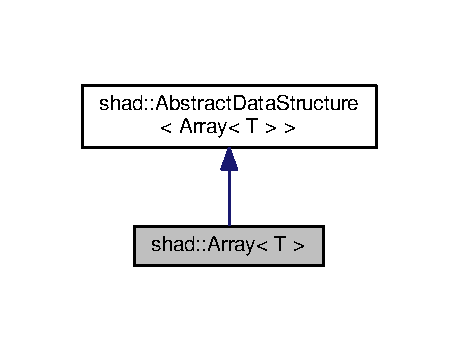
\includegraphics[width=220pt]{classshad_1_1Array__inherit__graph}
\end{center}
\end{figure}


Collaboration diagram for shad\-:\-:Array$<$ T $>$\-:
\nopagebreak
\begin{figure}[H]
\begin{center}
\leavevmode
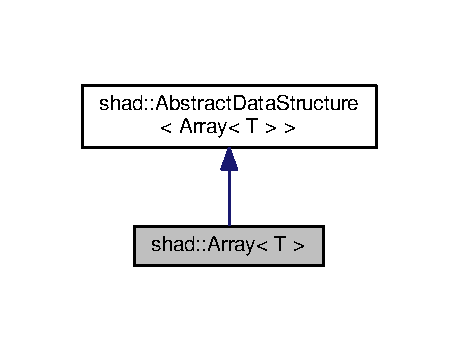
\includegraphics[width=220pt]{classshad_1_1Array__coll__graph}
\end{center}
\end{figure}
\subsection*{Public Types}
\begin{DoxyCompactItemize}
\item 
using \hyperlink{classshad_1_1Array_a69c0b0424c09d4779081e358548a3165}{Object\-I\-D} = typename \hyperlink{classshad_1_1AbstractDataStructure}{Abstract\-Data\-Structure}$<$ \hyperlink{classshad_1_1Array}{Array}$<$ T $>$$>$\-::\hyperlink{classshad_1_1Array_a69c0b0424c09d4779081e358548a3165}{Object\-I\-D}
\item 
using \hyperlink{classshad_1_1Array_a9d0f8fb34a90f8b9d232aa086ff75d2a}{Buffers\-Vector} = impl\-::\-Buffers\-Vector$<$ std\-::tuple$<$ size\-\_\-t, T $>$, \hyperlink{classshad_1_1Array}{Array}$<$ T $>$$>$
\item 
using \hyperlink{classshad_1_1Array_a5ff91c72815df47db60fc6ed44b01d46}{Shad\-Array\-Ptr} = typename \hyperlink{classshad_1_1AbstractDataStructure}{Abstract\-Data\-Structure}$<$ \hyperlink{classshad_1_1Array}{Array}$<$ T $>$$>$\-::\hyperlink{classshad_1_1AbstractDataStructure_a8bb29450966955c546d40421ce46316f}{Shared\-Ptr}
\end{DoxyCompactItemize}
\subsection*{Public Member Functions}
\begin{DoxyCompactItemize}
\item 
\hyperlink{classshad_1_1Array_a69c0b0424c09d4779081e358548a3165}{Object\-I\-D} \hyperlink{classshad_1_1Array_a6340a0b0ce2b34964e580a86f0c9cbcd}{Get\-Global\-I\-D} () const 
\begin{DoxyCompactList}\small\item\em Retrieve the Global Identifier. \end{DoxyCompactList}\item 
size\-\_\-t \hyperlink{classshad_1_1Array_ab6ebd2321e693fbcbf6ff6ec90a12f56}{Size} () const noexcept
\begin{DoxyCompactList}\small\item\em Return the size of the \hyperlink{classshad_1_1Array}{shad\-::\-Array}. \end{DoxyCompactList}\item 
void \hyperlink{classshad_1_1Array_ae90ba873251e3dd7afb36fc58a1aa648}{Insert\-At} (const size\-\_\-t pos, const T \&value)
\begin{DoxyCompactList}\small\item\em Synchronous insert method. \end{DoxyCompactList}\item 
void \hyperlink{classshad_1_1Array_a3f460d2e4d34fe22fa2ede421e668da0}{Insert\-At} (const size\-\_\-t pos, const T $\ast$values, const size\-\_\-t num\-Values)
\begin{DoxyCompactList}\small\item\em Synchronous bulk insert method. \end{DoxyCompactList}\item 
void \hyperlink{classshad_1_1Array_a0e145550478683482a1601031535c8cf}{Async\-Insert\-At} (\hyperlink{classshad_1_1rt_1_1Handle}{rt\-::\-Handle} \&handle, const size\-\_\-t pos, const T \&value)
\begin{DoxyCompactList}\small\item\em Asynchronous Insert method. \end{DoxyCompactList}\item 
void \hyperlink{classshad_1_1Array_af3e5d9c1664af29e635e1ed6c96eaf70}{Async\-Insert\-At} (\hyperlink{classshad_1_1rt_1_1Handle}{rt\-::\-Handle} \&handle, const size\-\_\-t pos, const T $\ast$values, const size\-\_\-t num\-Values)
\begin{DoxyCompactList}\small\item\em Asynchronous bulk insert method. \end{DoxyCompactList}\item 
void \hyperlink{classshad_1_1Array_ac684b1894e474db3e9fee060a1bd59bf}{Buffered\-Insert\-At} (const size\-\_\-t pos, const T \&value)
\begin{DoxyCompactList}\small\item\em Buffered insert method. \end{DoxyCompactList}\item 
void \hyperlink{classshad_1_1Array_a34c463d858d31e8090534405c7692580}{Buffered\-Async\-Insert\-At} (\hyperlink{classshad_1_1rt_1_1Handle}{rt\-::\-Handle} \&handle, const size\-\_\-t pos, const T \&value)
\begin{DoxyCompactList}\small\item\em Asynchronous buffered insert method. \end{DoxyCompactList}\item 
void \hyperlink{classshad_1_1Array_a80bdbc75aca1424f086305d9297dccec}{Wait\-For\-Buffered\-Insert} ()
\begin{DoxyCompactList}\small\item\em Finalize method for buffered insertions. \end{DoxyCompactList}\item 
T \hyperlink{classshad_1_1Array_a56085a958b519c523540a5e8babb8045}{At} (const size\-\_\-t pos)
\begin{DoxyCompactList}\small\item\em Lookup Method. \end{DoxyCompactList}\item 
void \hyperlink{classshad_1_1Array_a23fe4840cee746b5f54c118650139ed0}{Async\-At} (\hyperlink{classshad_1_1rt_1_1Handle}{rt\-::\-Handle} \&handle, const size\-\_\-t pos, T $\ast$result)
\begin{DoxyCompactList}\small\item\em Asynchronous Lookup Method. \end{DoxyCompactList}\item 
{\footnotesize template$<$typename Apply\-Fun\-T , typename... Args$>$ }\\void \hyperlink{classshad_1_1Array_a044795e62744280d74a0fc8933dc5b6c}{Apply} (const size\-\_\-t pos, Apply\-Fun\-T \&\&function, Args \&...args)
\begin{DoxyCompactList}\small\item\em Applies a user-\/defined function to an element. \end{DoxyCompactList}\item 
{\footnotesize template$<$typename Apply\-Fun\-T , typename... Args$>$ }\\void \hyperlink{classshad_1_1Array_a7761587f45d0059212091ba33366e4e6}{Async\-Apply} (\hyperlink{classshad_1_1rt_1_1Handle}{rt\-::\-Handle} \&handle, const size\-\_\-t pos, Apply\-Fun\-T \&\&function, Args \&...args)
\begin{DoxyCompactList}\small\item\em Asynchronously applies a user-\/defined function to an element. \end{DoxyCompactList}\item 
{\footnotesize template$<$typename Apply\-Fun\-T , typename... Args$>$ }\\void \hyperlink{classshad_1_1Array_a5136714d22b0efef01f6711e2ad2a8fc}{For\-Each\-In\-Range} (const size\-\_\-t first, const size\-\_\-t last, Apply\-Fun\-T \&\&function, Args \&...args)
\begin{DoxyCompactList}\small\item\em Applies a user-\/defined function to every element in the specified range. \end{DoxyCompactList}\item 
{\footnotesize template$<$typename Apply\-Fun\-T , typename... Args$>$ }\\void \hyperlink{classshad_1_1Array_a993d7eb96221277f74c6fb4c36f36f8e}{Async\-For\-Each\-In\-Range} (\hyperlink{classshad_1_1rt_1_1Handle}{rt\-::\-Handle} \&handle, const size\-\_\-t first, const size\-\_\-t last, Apply\-Fun\-T \&\&function, Args \&...args)
\begin{DoxyCompactList}\small\item\em Asynchronously applies a user-\/defined function to every element in the specified range. \end{DoxyCompactList}\item 
{\footnotesize template$<$typename Apply\-Fun\-T , typename... Args$>$ }\\void \hyperlink{classshad_1_1Array_a6fd05a7fd2e8ef73ed288f5c1bfcf171}{For\-Each} (Apply\-Fun\-T \&\&function, Args \&...args)
\begin{DoxyCompactList}\small\item\em Applies a user-\/defined function to every element. \end{DoxyCompactList}\item 
{\footnotesize template$<$typename Apply\-Fun\-T , typename... Args$>$ }\\void \hyperlink{classshad_1_1Array_a076303cbecce5e29fadd0a4333428efa}{Async\-For\-Each} (\hyperlink{classshad_1_1rt_1_1Handle}{rt\-::\-Handle} \&handle, Apply\-Fun\-T \&\&function, Args \&...args)
\begin{DoxyCompactList}\small\item\em Asynchronously applies a user-\/defined function to every element. \end{DoxyCompactList}\item 
void \hyperlink{classshad_1_1Array_a98bd6440ea4037335356cd6cc95a0cde}{Buffer\-Entry\-Insert} (const std\-::tuple$<$ size\-\_\-t, T $>$ entry)
\end{DoxyCompactItemize}
\subsection*{Static Public Member Functions}
\begin{DoxyCompactItemize}
\item 
static \hyperlink{classshad_1_1Array_a5ff91c72815df47db60fc6ed44b01d46}{Shad\-Array\-Ptr} \hyperlink{classshad_1_1Array_a4ff830861f0ace4bf0a5e39e400b50f8}{Create} (size\-\_\-t size, const T \&init\-Value)
\begin{DoxyCompactList}\small\item\em Create method. \end{DoxyCompactList}\end{DoxyCompactItemize}
\subsection*{Static Public Attributes}
\begin{DoxyCompactItemize}
\item 
static constexpr size\-\_\-t \hyperlink{classshad_1_1Array_af4d2703149c199273eae358d1bcd8ade}{k\-Max\-Chunk\-Size}
\end{DoxyCompactItemize}
\subsection*{Protected Member Functions}
\begin{DoxyCompactItemize}
\item 
\hyperlink{classshad_1_1Array_a651339c6f76aea1b4f5120ebfc46bdd0}{Array} (\hyperlink{classshad_1_1Array_a69c0b0424c09d4779081e358548a3165}{Object\-I\-D} oid, size\-\_\-t size, const T \&init\-Value)
\end{DoxyCompactItemize}
\subsection*{Friends}
\begin{DoxyCompactItemize}
\item 
{\footnotesize template$<$typename $>$ }\\class \hyperlink{classshad_1_1Array_ab18afa4496cc863ddc11bab94b2adf57}{Abstract\-Data\-Structure}
\end{DoxyCompactItemize}
\subsection*{Additional Inherited Members}


\subsection{Detailed Description}
\subsubsection*{template$<$typename T$>$class shad\-::\-Array$<$ T $>$}

The \hyperlink{classshad_1_1Array}{Array} data structure. 

S\-H\-A\-D's \hyperlink{classshad_1_1Array}{Array} is a fixed size distributed container.

\begin{DoxyWarning}{Warning}
obects of type T need to be trivially copiable.
\end{DoxyWarning}

\begin{DoxyTemplParams}{Template Parameters}
{\em T} & type of the entries stored in the \hyperlink{classshad_1_1Array}{Array}. \\
\hline
\end{DoxyTemplParams}


\subsection{Member Typedef Documentation}
\hypertarget{classshad_1_1Array_a9d0f8fb34a90f8b9d232aa086ff75d2a}{\index{shad\-::\-Array@{shad\-::\-Array}!Buffers\-Vector@{Buffers\-Vector}}
\index{Buffers\-Vector@{Buffers\-Vector}!shad::Array@{shad\-::\-Array}}
\subsubsection[{Buffers\-Vector}]{\setlength{\rightskip}{0pt plus 5cm}template$<$typename T$>$ using {\bf shad\-::\-Array}$<$ T $>$\-::{\bf Buffers\-Vector} =  impl\-::\-Buffers\-Vector$<$std\-::tuple$<$size\-\_\-t, T$>$, {\bf Array}$<$T$>$$>$}}\label{classshad_1_1Array_a9d0f8fb34a90f8b9d232aa086ff75d2a}
\hypertarget{classshad_1_1Array_a69c0b0424c09d4779081e358548a3165}{\index{shad\-::\-Array@{shad\-::\-Array}!Object\-I\-D@{Object\-I\-D}}
\index{Object\-I\-D@{Object\-I\-D}!shad::Array@{shad\-::\-Array}}
\subsubsection[{Object\-I\-D}]{\setlength{\rightskip}{0pt plus 5cm}template$<$typename T$>$ using {\bf shad\-::\-Array}$<$ T $>$\-::{\bf Object\-I\-D} =  typename {\bf Abstract\-Data\-Structure}$<${\bf Array}$<$T$>$$>$\-::{\bf Object\-I\-D}}}\label{classshad_1_1Array_a69c0b0424c09d4779081e358548a3165}
\hypertarget{classshad_1_1Array_a5ff91c72815df47db60fc6ed44b01d46}{\index{shad\-::\-Array@{shad\-::\-Array}!Shad\-Array\-Ptr@{Shad\-Array\-Ptr}}
\index{Shad\-Array\-Ptr@{Shad\-Array\-Ptr}!shad::Array@{shad\-::\-Array}}
\subsubsection[{Shad\-Array\-Ptr}]{\setlength{\rightskip}{0pt plus 5cm}template$<$typename T$>$ using {\bf shad\-::\-Array}$<$ T $>$\-::{\bf Shad\-Array\-Ptr} =  typename {\bf Abstract\-Data\-Structure}$<${\bf Array}$<$T$>$$>$\-::{\bf Shared\-Ptr}}}\label{classshad_1_1Array_a5ff91c72815df47db60fc6ed44b01d46}


\subsection{Constructor \& Destructor Documentation}
\hypertarget{classshad_1_1Array_a651339c6f76aea1b4f5120ebfc46bdd0}{\index{shad\-::\-Array@{shad\-::\-Array}!Array@{Array}}
\index{Array@{Array}!shad::Array@{shad\-::\-Array}}
\subsubsection[{Array}]{\setlength{\rightskip}{0pt plus 5cm}template$<$typename T$>$ {\bf shad\-::\-Array}$<$ T $>$\-::{\bf Array} (
\begin{DoxyParamCaption}
\item[{{\bf Object\-I\-D}}]{oid, }
\item[{size\-\_\-t}]{size, }
\item[{const T \&}]{init\-Value}
\end{DoxyParamCaption}
)\hspace{0.3cm}{\ttfamily [inline]}, {\ttfamily [protected]}}}\label{classshad_1_1Array_a651339c6f76aea1b4f5120ebfc46bdd0}


\subsection{Member Function Documentation}
\hypertarget{classshad_1_1Array_a044795e62744280d74a0fc8933dc5b6c}{\index{shad\-::\-Array@{shad\-::\-Array}!Apply@{Apply}}
\index{Apply@{Apply}!shad::Array@{shad\-::\-Array}}
\subsubsection[{Apply}]{\setlength{\rightskip}{0pt plus 5cm}template$<$typename T $>$ template$<$typename Apply\-Fun\-T , typename... Args$>$ void {\bf shad\-::\-Array}$<$ T $>$\-::Apply (
\begin{DoxyParamCaption}
\item[{const size\-\_\-t}]{pos, }
\item[{Apply\-Fun\-T \&\&}]{function, }
\item[{Args \&...}]{args}
\end{DoxyParamCaption}
)}}\label{classshad_1_1Array_a044795e62744280d74a0fc8933dc5b6c}


Applies a user-\/defined function to an element. 

Applies a user-\/defined function to the element at the specified position.

Typical usage\-: 
\begin{DoxyCode}
\textcolor{keywordtype}{void} fn(\textcolor{keywordtype}{size\_t} i, \textcolor{keywordtype}{size\_t}& elem, \textcolor{keywordtype}{size\_t} & incr) \{ \textcolor{comment}{/* do something */} \}
...
auto edsPtr = \hyperlink{classshad_1_1Array_a4ff830861f0ace4bf0a5e39e400b50f8}{shad::Array<size\_t>::Create}(kArraySize, kInitValue);
\textcolor{keywordflow}{for} (\textcolor{keywordtype}{size\_t} i = 0; i < kArraySize; i++) \{
  edsPtr->Apply(i, fn, kInitValue);
\}
...
\end{DoxyCode}



\begin{DoxyTemplParams}{Template Parameters}
{\em Apply\-Fun\-T} & User-\/defined function type. The function prototype must be\-: 
\begin{DoxyCode}
void(\textcolor{keywordtype}{size\_t}, T&, Args& args);
\end{DoxyCode}
 \\
\hline
{\em ...\-Args} & Types of the function arguments.\\
\hline
\end{DoxyTemplParams}

\begin{DoxyParams}[1]{Parameters}
\mbox{\tt in}  & {\em pos} & The target position. \\
\hline
\mbox{\tt in}  & {\em function} & The function to apply. \\
\hline
\mbox{\tt in}  & {\em args} & The function arguments. \\
\hline
\end{DoxyParams}
\hypertarget{classshad_1_1Array_a7761587f45d0059212091ba33366e4e6}{\index{shad\-::\-Array@{shad\-::\-Array}!Async\-Apply@{Async\-Apply}}
\index{Async\-Apply@{Async\-Apply}!shad::Array@{shad\-::\-Array}}
\subsubsection[{Async\-Apply}]{\setlength{\rightskip}{0pt plus 5cm}template$<$typename T $>$ template$<$typename Apply\-Fun\-T , typename... Args$>$ void {\bf shad\-::\-Array}$<$ T $>$\-::Async\-Apply (
\begin{DoxyParamCaption}
\item[{{\bf rt\-::\-Handle} \&}]{handle, }
\item[{const size\-\_\-t}]{pos, }
\item[{Apply\-Fun\-T \&\&}]{function, }
\item[{Args \&...}]{args}
\end{DoxyParamCaption}
)}}\label{classshad_1_1Array_a7761587f45d0059212091ba33366e4e6}


Asynchronously applies a user-\/defined function to an element. 

Asynchronously applies a user-\/defined function to the element at the specified position.

\begin{DoxyWarning}{Warning}
Asynchronous operations are guaranteed to have completed only after calling the \hyperlink{namespaceshad_1_1rt_a6ea1d3672bac3a80032863b6732a0c0a}{rt\-::wait\-For\-Completion(rt\-::\-Handle \&handle)} method.
\end{DoxyWarning}
Typical usage\-: 
\begin{DoxyCode}
\textcolor{keywordtype}{void} fn(\hyperlink{classshad_1_1rt_1_1Handle}{shad::rt::Handle}&, \textcolor{keywordtype}{size\_t} i, \textcolor{keywordtype}{size\_t}& elem, \textcolor{keywordtype}{size\_t} & incr) \{
  \textcolor{comment}{/* do something */}
\}
...
auto arrayPtr = \hyperlink{classshad_1_1Array_a4ff830861f0ace4bf0a5e39e400b50f8}{shad::Array<size\_t>::Create}(kArraySize, kInitValue);
\hyperlink{classshad_1_1rt_1_1Handle}{shad::rt::Handle} handle;
\textcolor{keywordflow}{for} (\textcolor{keywordtype}{size\_t} i = 0; i < kArraySize; i++) \{
  arrayPtr->AsyncApply(handle, i, fn, kInitValue);
\}
\hyperlink{namespaceshad_1_1rt_a6ea1d3672bac3a80032863b6732a0c0a}{shad::rt::waitForCompletion}(handle);
...
\end{DoxyCode}



\begin{DoxyTemplParams}{Template Parameters}
{\em Apply\-Fun\-T} & User-\/defined function type. The function prototype must be\-: 
\begin{DoxyCode}
void(\hyperlink{classshad_1_1rt_1_1Handle}{shad::rt::Handle}&, \textcolor{keywordtype}{size\_t}, T&, Args& args);
\end{DoxyCode}
 \\
\hline
{\em ...\-Args} & Types of the function arguments.\\
\hline
\end{DoxyTemplParams}

\begin{DoxyParams}[1]{Parameters}
\mbox{\tt in,out}  & {\em handle} & Reference to the handle to be used to wait for completion. \\
\hline
\mbox{\tt in}  & {\em pos} & The target position. \\
\hline
\mbox{\tt in}  & {\em function} & The function to apply. \\
\hline
\mbox{\tt in}  & {\em args} & The function arguments. \\
\hline
\end{DoxyParams}
\hypertarget{classshad_1_1Array_a23fe4840cee746b5f54c118650139ed0}{\index{shad\-::\-Array@{shad\-::\-Array}!Async\-At@{Async\-At}}
\index{Async\-At@{Async\-At}!shad::Array@{shad\-::\-Array}}
\subsubsection[{Async\-At}]{\setlength{\rightskip}{0pt plus 5cm}template$<$typename T $>$ void {\bf shad\-::\-Array}$<$ T $>$\-::Async\-At (
\begin{DoxyParamCaption}
\item[{{\bf rt\-::\-Handle} \&}]{handle, }
\item[{const size\-\_\-t}]{pos, }
\item[{T $\ast$}]{result}
\end{DoxyParamCaption}
)}}\label{classshad_1_1Array_a23fe4840cee746b5f54c118650139ed0}


Asynchronous Lookup Method. 

Retireve an element at a given position asynchronously.

\begin{DoxyWarning}{Warning}
Asynchronous operations are guaranteed to have completed only after calling the \hyperlink{namespaceshad_1_1rt_a6ea1d3672bac3a80032863b6732a0c0a}{rt\-::wait\-For\-Completion(rt\-::\-Handle \&handle)} method.
\end{DoxyWarning}
Typical usage\-: 
\begin{DoxyCode}
\textcolor{keyword}{auto} arrayPtr = \hyperlink{classshad_1_1Array_a4ff830861f0ace4bf0a5e39e400b50f8}{shad::Array<size\_t>::Create}(kArraySize, kInitValue);
\textcolor{comment}{// ... fill the array with useful values ...}

std::vector<size\_t> top(k);
\hyperlink{classshad_1_1rt_1_1Handle}{shad::rt::Handle} handle;
\textcolor{keywordflow}{for} (\textcolor{keywordtype}{size\_t} i = 0; i < k; ++i)
  arrayPtr->AsyncAt(i, &top[i]);

\hyperlink{namespaceshad_1_1rt_a6ea1d3672bac3a80032863b6732a0c0a}{shad::rt::waitForCompletion}(handle);
\textcolor{keywordflow}{for} (\textcolor{keyword}{auto} v : top)
  PrintValue(v);
\end{DoxyCode}



\begin{DoxyParams}[1]{Parameters}
\mbox{\tt in,out}  & {\em handle} & The handle to be used to wait for completion. \\
\hline
\mbox{\tt in}  & {\em pos} & The target position. \\
\hline
\mbox{\tt out}  & {\em result} & pointer to the region where the element value is written; result must point to a valid memory allocation. \\
\hline
\end{DoxyParams}
\hypertarget{classshad_1_1Array_a076303cbecce5e29fadd0a4333428efa}{\index{shad\-::\-Array@{shad\-::\-Array}!Async\-For\-Each@{Async\-For\-Each}}
\index{Async\-For\-Each@{Async\-For\-Each}!shad::Array@{shad\-::\-Array}}
\subsubsection[{Async\-For\-Each}]{\setlength{\rightskip}{0pt plus 5cm}template$<$typename T $>$ template$<$typename Apply\-Fun\-T , typename... Args$>$ void {\bf shad\-::\-Array}$<$ T $>$\-::Async\-For\-Each (
\begin{DoxyParamCaption}
\item[{{\bf rt\-::\-Handle} \&}]{handle, }
\item[{Apply\-Fun\-T \&\&}]{function, }
\item[{Args \&...}]{args}
\end{DoxyParamCaption}
)}}\label{classshad_1_1Array_a076303cbecce5e29fadd0a4333428efa}


Asynchronously applies a user-\/defined function to every element. 

Asynchronously applies a user-\/defined function to all the elements.

\begin{DoxyWarning}{Warning}
Asynchronous operations are guaranteed to have completed only after calling the \hyperlink{namespaceshad_1_1rt_a6ea1d3672bac3a80032863b6732a0c0a}{rt\-::wait\-For\-Completion(rt\-::\-Handle \&handle)} method.
\end{DoxyWarning}
Typical usage\-: 
\begin{DoxyCode}
\textcolor{keywordtype}{void} fn(\hyperlink{classshad_1_1rt_1_1Handle}{shad::rt::Handle}&, \textcolor{keywordtype}{size\_t} i, \textcolor{keywordtype}{size\_t}& elem, \textcolor{keywordtype}{size\_t}& incr) \{
  \textcolor{comment}{/* do something */}
\}
...
auto arrayPtr = \hyperlink{classshad_1_1Array_a4ff830861f0ace4bf0a5e39e400b50f8}{shad::Array<size\_t>::Create}(kArraySize, kInitValue);
rt::Handle handle;
arrayPtr->AsyncForEach(handle, fn, someValue);
...
shad::rt::waitForCompletion(handle);
...
\end{DoxyCode}



\begin{DoxyTemplParams}{Template Parameters}
{\em Apply\-Fun\-T} & User-\/defined function type. The function prototype must be\-: 
\begin{DoxyCode}
void(\hyperlink{classshad_1_1rt_1_1Handle}{shad::rt::Handle}&, \textcolor{keywordtype}{size\_t} pos, T&, Args& args);
\end{DoxyCode}
 \\
\hline
{\em ...\-Args} & Types of the function arguments.\\
\hline
\end{DoxyTemplParams}

\begin{DoxyParams}[1]{Parameters}
\mbox{\tt in,out}  & {\em handle} & The handle to be used to wait for completion. \\
\hline
\mbox{\tt in}  & {\em function} & The function to apply. \\
\hline
\mbox{\tt in}  & {\em args} & The function arguments. \\
\hline
\end{DoxyParams}
\hypertarget{classshad_1_1Array_a993d7eb96221277f74c6fb4c36f36f8e}{\index{shad\-::\-Array@{shad\-::\-Array}!Async\-For\-Each\-In\-Range@{Async\-For\-Each\-In\-Range}}
\index{Async\-For\-Each\-In\-Range@{Async\-For\-Each\-In\-Range}!shad::Array@{shad\-::\-Array}}
\subsubsection[{Async\-For\-Each\-In\-Range}]{\setlength{\rightskip}{0pt plus 5cm}template$<$typename T $>$ template$<$typename Apply\-Fun\-T , typename... Args$>$ void {\bf shad\-::\-Array}$<$ T $>$\-::Async\-For\-Each\-In\-Range (
\begin{DoxyParamCaption}
\item[{{\bf rt\-::\-Handle} \&}]{handle, }
\item[{const size\-\_\-t}]{first, }
\item[{const size\-\_\-t}]{last, }
\item[{Apply\-Fun\-T \&\&}]{function, }
\item[{Args \&...}]{args}
\end{DoxyParamCaption}
)}}\label{classshad_1_1Array_a993d7eb96221277f74c6fb4c36f36f8e}


Asynchronously applies a user-\/defined function to every element in the specified range. 

Asynchronously applies a user-\/defined function to all the elements in the specified range of positions.

\begin{DoxyWarning}{Warning}
Asynchronous operations are guaranteed to have completed only after calling the \hyperlink{namespaceshad_1_1rt_a6ea1d3672bac3a80032863b6732a0c0a}{rt\-::wait\-For\-Completion(rt\-::\-Handle \&handle)} method.
\end{DoxyWarning}
Typical usage\-: 
\begin{DoxyCode}
\textcolor{keywordtype}{void} fn(\hyperlink{classshad_1_1rt_1_1Handle}{shad::rt::Handle}&, \textcolor{keywordtype}{size\_t} i, \textcolor{keywordtype}{size\_t}& elem, \textcolor{keywordtype}{size\_t}& incr) \{
  \textcolor{comment}{/* do something */}
\}
...
auto arrayPtr = \hyperlink{classshad_1_1Array_a4ff830861f0ace4bf0a5e39e400b50f8}{shad::Array<size\_t>::Create}(kArraySize, kInitValue);
\hyperlink{classshad_1_1rt_1_1Handle}{shad::rt::Handle} handle;
arrayPtr->AsyncForEachInRange(handle, 0, kArraySize, fn, kInitValue);
...
rt::waitForCompletion(handle);
...
\end{DoxyCode}



\begin{DoxyTemplParams}{Template Parameters}
{\em Apply\-Fun\-T} & User-\/defined function type. The function prototype must be\-: 
\begin{DoxyCode}
void(\hyperlink{classshad_1_1rt_1_1Handle}{shad::rt::Handle}&, \textcolor{keywordtype}{size\_t}, T&, Args& args);
\end{DoxyCode}
 \\
\hline
{\em ...\-Args} & Types of the function arguments.\\
\hline
\end{DoxyTemplParams}

\begin{DoxyParams}[1]{Parameters}
\mbox{\tt in,out}  & {\em handle} & Reference to the handle to be used to wait for completion. \\
\hline
\mbox{\tt in}  & {\em first} & The first position of the range. \\
\hline
\mbox{\tt in}  & {\em last} & The last position of the range. \\
\hline
\mbox{\tt in}  & {\em function} & The function to apply. \\
\hline
\mbox{\tt in}  & {\em args} & The function arguments. \\
\hline
\end{DoxyParams}
\hypertarget{classshad_1_1Array_a0e145550478683482a1601031535c8cf}{\index{shad\-::\-Array@{shad\-::\-Array}!Async\-Insert\-At@{Async\-Insert\-At}}
\index{Async\-Insert\-At@{Async\-Insert\-At}!shad::Array@{shad\-::\-Array}}
\subsubsection[{Async\-Insert\-At}]{\setlength{\rightskip}{0pt plus 5cm}template$<$typename T $>$ void {\bf shad\-::\-Array}$<$ T $>$\-::Async\-Insert\-At (
\begin{DoxyParamCaption}
\item[{{\bf rt\-::\-Handle} \&}]{handle, }
\item[{const size\-\_\-t}]{pos, }
\item[{const T \&}]{value}
\end{DoxyParamCaption}
)}}\label{classshad_1_1Array_a0e145550478683482a1601031535c8cf}


Asynchronous Insert method. 

Asynchronously inserts an element at the specified position.

\begin{DoxyWarning}{Warning}
Asynchronous operations are guaranteed to have completed only after calling the \hyperlink{namespaceshad_1_1rt_a6ea1d3672bac3a80032863b6732a0c0a}{rt\-::wait\-For\-Completion(rt\-::\-Handle\& handle)} method.
\end{DoxyWarning}
Typical usage\-: 
\begin{DoxyCode}
\hyperlink{classshad_1_1rt_1_1Handle}{shad::rt::Handle} handle;
\textcolor{keyword}{auto} arrayPtr = \hyperlink{classshad_1_1Array_a4ff830861f0ace4bf0a5e39e400b50f8}{shad::Array<size\_t>::Create}(kArraySize, kInitValue);
\textcolor{keywordflow}{for} (\textcolor{keywordtype}{size\_t} i = 0; i < kArraySize; i++) \{
  arrayPtr->AsyncInsertAt(handle, i, i+1);
\}
\textcolor{comment}{// ... more work here and then finally wait.}
\hyperlink{namespaceshad_1_1rt_a6ea1d3672bac3a80032863b6732a0c0a}{shad::rt::waitForCompletion}(handle);
\end{DoxyCode}



\begin{DoxyParams}[1]{Parameters}
\mbox{\tt in,out}  & {\em handle} & The handle to be used to wait for completion. \\
\hline
\mbox{\tt in}  & {\em pos} & The target position. \\
\hline
\mbox{\tt in}  & {\em value} & The value to be inserted. \\
\hline
\end{DoxyParams}
\hypertarget{classshad_1_1Array_af3e5d9c1664af29e635e1ed6c96eaf70}{\index{shad\-::\-Array@{shad\-::\-Array}!Async\-Insert\-At@{Async\-Insert\-At}}
\index{Async\-Insert\-At@{Async\-Insert\-At}!shad::Array@{shad\-::\-Array}}
\subsubsection[{Async\-Insert\-At}]{\setlength{\rightskip}{0pt plus 5cm}template$<$typename T $>$ void {\bf shad\-::\-Array}$<$ T $>$\-::Async\-Insert\-At (
\begin{DoxyParamCaption}
\item[{{\bf rt\-::\-Handle} \&}]{handle, }
\item[{const size\-\_\-t}]{pos, }
\item[{const T $\ast$}]{values, }
\item[{const size\-\_\-t}]{num\-Values}
\end{DoxyParamCaption}
)}}\label{classshad_1_1Array_af3e5d9c1664af29e635e1ed6c96eaf70}


Asynchronous bulk insert method. 

Asynchronously inserts multiple elements starting at the specified position.

Typical usage\-: 
\begin{DoxyCode}
std::vector<size\_t> values(10, 1);
\textcolor{keyword}{auto} arrayPtr = \hyperlink{classshad_1_1Array_a4ff830861f0ace4bf0a5e39e400b50f8}{shad::Array<size\_t>::Create}(kArraySize, kInitValue);

\hyperlink{classshad_1_1rt_1_1Handle}{shad::rt::Handle} handle;
arrayPtr->AsyncInsertAt(handle, 0, values.data(), values.size());
\textcolor{comment}{// ... more work here and then finally wait.}
\hyperlink{namespaceshad_1_1rt_a6ea1d3672bac3a80032863b6732a0c0a}{shad::rt::waitForCompletion}(handle);;
\end{DoxyCode}



\begin{DoxyParams}[1]{Parameters}
\mbox{\tt in,out}  & {\em handle} & The handle to be used to wait for completion. \\
\hline
\mbox{\tt in}  & {\em pos} & The target position. \\
\hline
\mbox{\tt in}  & {\em values} & Pointer to the values to be inserted. \\
\hline
\mbox{\tt in}  & {\em num\-Values} & Number of values to be inserted. \\
\hline
\end{DoxyParams}
\hypertarget{classshad_1_1Array_a56085a958b519c523540a5e8babb8045}{\index{shad\-::\-Array@{shad\-::\-Array}!At@{At}}
\index{At@{At}!shad::Array@{shad\-::\-Array}}
\subsubsection[{At}]{\setlength{\rightskip}{0pt plus 5cm}template$<$typename T $>$ T {\bf shad\-::\-Array}$<$ T $>$\-::At (
\begin{DoxyParamCaption}
\item[{const size\-\_\-t}]{pos}
\end{DoxyParamCaption}
)}}\label{classshad_1_1Array_a56085a958b519c523540a5e8babb8045}


Lookup Method. 

Retireve an element at a given position.

Typical usage\-: 
\begin{DoxyCode}
\textcolor{keyword}{auto} arrayPtr = \hyperlink{classshad_1_1Array_a4ff830861f0ace4bf0a5e39e400b50f8}{shad::Array<size\_t>::Create}(kArraySize, kInitValue);
\textcolor{comment}{// ... fill the array with useful values ...}

\textcolor{keywordflow}{for} (\textcolor{keywordtype}{size\_t} i = 0; i < arrayPtr->Size(); ++i)
  PrintValue(arrayPtr->At(i));  \textcolor{comment}{// Don't do this !}
\end{DoxyCode}



\begin{DoxyParams}[1]{Parameters}
\mbox{\tt in}  & {\em pos} & The target position. \\
\hline
\end{DoxyParams}
\begin{DoxyReturn}{Returns}
The value of the element at position pos. 
\end{DoxyReturn}
\hypertarget{classshad_1_1Array_a34c463d858d31e8090534405c7692580}{\index{shad\-::\-Array@{shad\-::\-Array}!Buffered\-Async\-Insert\-At@{Buffered\-Async\-Insert\-At}}
\index{Buffered\-Async\-Insert\-At@{Buffered\-Async\-Insert\-At}!shad::Array@{shad\-::\-Array}}
\subsubsection[{Buffered\-Async\-Insert\-At}]{\setlength{\rightskip}{0pt plus 5cm}template$<$typename T $>$ void {\bf shad\-::\-Array}$<$ T $>$\-::Buffered\-Async\-Insert\-At (
\begin{DoxyParamCaption}
\item[{{\bf rt\-::\-Handle} \&}]{handle, }
\item[{const size\-\_\-t}]{pos, }
\item[{const T \&}]{value}
\end{DoxyParamCaption}
)}}\label{classshad_1_1Array_a34c463d858d31e8090534405c7692580}


Asynchronous buffered insert method. 

Asynchronously inserts an element at the specified position, using aggregation buffers.

\begin{DoxyWarning}{Warning}
asynchronous buffered insertions are finalized only after calling the \hyperlink{namespaceshad_1_1rt_a6ea1d3672bac3a80032863b6732a0c0a}{rt\-::wait\-For\-Completion(rt\-::\-Handle \&handle)} method {\bfseries and} the \hyperlink{classshad_1_1Array_a80bdbc75aca1424f086305d9297dccec}{Wait\-For\-Buffered\-Insert()} method, in this order.
\end{DoxyWarning}
Typical usage\-: 
\begin{DoxyCode}
\textcolor{keyword}{auto} arrayPtr = \hyperlink{classshad_1_1Array_a4ff830861f0ace4bf0a5e39e400b50f8}{shad::Array<size\_t>::Create}(kArraySize, kInitValue);

\hyperlink{classshad_1_1rt_1_1Handle}{shad::rt::Handle} handle;
\textcolor{keywordflow}{for} (\textcolor{keywordtype}{size\_t} i = 0; i < kArraySize; i++) \{
  arrayPtr->BufferedAsyncInsertAt(handle, i, i+1);
\}
\textcolor{comment}{// ... more work here and then finally wait.}
\hyperlink{namespaceshad_1_1rt_a6ea1d3672bac3a80032863b6732a0c0a}{shad::rt::waitForCompletion}(handle);
arrayPtr->WaitForBufferedInsert();
\end{DoxyCode}



\begin{DoxyParams}[1]{Parameters}
\mbox{\tt in,out}  & {\em handle} & The handle to be used to wait for completion. \\
\hline
\mbox{\tt in}  & {\em pos} & The target position. \\
\hline
\mbox{\tt in}  & {\em value} & The value to be inserted. \\
\hline
\end{DoxyParams}
\hypertarget{classshad_1_1Array_ac684b1894e474db3e9fee060a1bd59bf}{\index{shad\-::\-Array@{shad\-::\-Array}!Buffered\-Insert\-At@{Buffered\-Insert\-At}}
\index{Buffered\-Insert\-At@{Buffered\-Insert\-At}!shad::Array@{shad\-::\-Array}}
\subsubsection[{Buffered\-Insert\-At}]{\setlength{\rightskip}{0pt plus 5cm}template$<$typename T $>$ void {\bf shad\-::\-Array}$<$ T $>$\-::Buffered\-Insert\-At (
\begin{DoxyParamCaption}
\item[{const size\-\_\-t}]{pos, }
\item[{const T \&}]{value}
\end{DoxyParamCaption}
)}}\label{classshad_1_1Array_ac684b1894e474db3e9fee060a1bd59bf}


Buffered insert method. 

Inserts an element at the specified position, using aggregation buffers.

\begin{DoxyWarning}{Warning}
Insertions are finalized only after calling the \hyperlink{classshad_1_1Array_a80bdbc75aca1424f086305d9297dccec}{Wait\-For\-Buffered\-Insert()} method.
\end{DoxyWarning}
Typical usage\-: 
\begin{DoxyCode}
\textcolor{keyword}{auto} arrayPtr = \hyperlink{classshad_1_1Array_a4ff830861f0ace4bf0a5e39e400b50f8}{shad::Array<size\_t>::Create}(kArraySize, kInitValue);
\textcolor{keywordflow}{for} (\textcolor{keywordtype}{size\_t} i = 0; i < kArraySize; i++) \{
  arrayPtr->BufferedInsertAt(i, i+1);
\}
arrayPtr->WaitForBufferedInsert();
\end{DoxyCode}



\begin{DoxyParams}[1]{Parameters}
\mbox{\tt in}  & {\em pos} & The target position. \\
\hline
\mbox{\tt in}  & {\em value} & The value of the element to be inserted. \\
\hline
\end{DoxyParams}
\hypertarget{classshad_1_1Array_a98bd6440ea4037335356cd6cc95a0cde}{\index{shad\-::\-Array@{shad\-::\-Array}!Buffer\-Entry\-Insert@{Buffer\-Entry\-Insert}}
\index{Buffer\-Entry\-Insert@{Buffer\-Entry\-Insert}!shad::Array@{shad\-::\-Array}}
\subsubsection[{Buffer\-Entry\-Insert}]{\setlength{\rightskip}{0pt plus 5cm}template$<$typename T$>$ void {\bf shad\-::\-Array}$<$ T $>$\-::Buffer\-Entry\-Insert (
\begin{DoxyParamCaption}
\item[{const std\-::tuple$<$ size\-\_\-t, T $>$}]{entry}
\end{DoxyParamCaption}
)\hspace{0.3cm}{\ttfamily [inline]}}}\label{classshad_1_1Array_a98bd6440ea4037335356cd6cc95a0cde}
\hypertarget{classshad_1_1Array_a4ff830861f0ace4bf0a5e39e400b50f8}{\index{shad\-::\-Array@{shad\-::\-Array}!Create@{Create}}
\index{Create@{Create}!shad::Array@{shad\-::\-Array}}
\subsubsection[{Create}]{\setlength{\rightskip}{0pt plus 5cm}template$<$typename T$>$ static {\bf Shad\-Array\-Ptr} {\bf shad\-::\-Array}$<$ T $>$\-::Create (
\begin{DoxyParamCaption}
\item[{size\-\_\-t}]{size, }
\item[{const T \&}]{init\-Value}
\end{DoxyParamCaption}
)\hspace{0.3cm}{\ttfamily [static]}}}\label{classshad_1_1Array_a4ff830861f0ace4bf0a5e39e400b50f8}


Create method. 

Creates a new array instance.


\begin{DoxyParams}{Parameters}
{\em size} & The size of the array.. \\
\hline
{\em init\-Value} & Initialization value. \\
\hline
\end{DoxyParams}
\begin{DoxyReturn}{Returns}
A shared pointer to the newly created array instance. 
\end{DoxyReturn}
\hypertarget{classshad_1_1Array_a6fd05a7fd2e8ef73ed288f5c1bfcf171}{\index{shad\-::\-Array@{shad\-::\-Array}!For\-Each@{For\-Each}}
\index{For\-Each@{For\-Each}!shad::Array@{shad\-::\-Array}}
\subsubsection[{For\-Each}]{\setlength{\rightskip}{0pt plus 5cm}template$<$typename T $>$ template$<$typename Apply\-Fun\-T , typename... Args$>$ void {\bf shad\-::\-Array}$<$ T $>$\-::For\-Each (
\begin{DoxyParamCaption}
\item[{Apply\-Fun\-T \&\&}]{function, }
\item[{Args \&...}]{args}
\end{DoxyParamCaption}
)}}\label{classshad_1_1Array_a6fd05a7fd2e8ef73ed288f5c1bfcf171}


Applies a user-\/defined function to every element. 

Applies a user-\/defined function to all the elements.

Typical usage\-: 
\begin{DoxyCode}
\textcolor{keywordtype}{void} fn(\textcolor{keywordtype}{size\_t} i, \textcolor{keywordtype}{size\_t}& elem, \textcolor{keywordtype}{size\_t}& incr) \{
  \textcolor{comment}{/* do something */}
\}
...
auto arrayPtr = \hyperlink{classshad_1_1Array_a4ff830861f0ace4bf0a5e39e400b50f8}{shad::Array<size\_t>::Create}(kArraySize, kInitValue);
arrayPtr->ForEach(fn, someValue);
\end{DoxyCode}



\begin{DoxyTemplParams}{Template Parameters}
{\em Apply\-Fun\-T} & User-\/defined function type. The function prototype must be\-: 
\begin{DoxyCode}
void(\textcolor{keywordtype}{size\_t} pos, T&, Args& args);
\end{DoxyCode}
 \\
\hline
{\em ...\-Args} & Types of the function arguments.\\
\hline
\end{DoxyTemplParams}

\begin{DoxyParams}[1]{Parameters}
\mbox{\tt in}  & {\em function} & The function to apply. \\
\hline
\mbox{\tt in}  & {\em args} & The function arguments. \\
\hline
\end{DoxyParams}
\hypertarget{classshad_1_1Array_a5136714d22b0efef01f6711e2ad2a8fc}{\index{shad\-::\-Array@{shad\-::\-Array}!For\-Each\-In\-Range@{For\-Each\-In\-Range}}
\index{For\-Each\-In\-Range@{For\-Each\-In\-Range}!shad::Array@{shad\-::\-Array}}
\subsubsection[{For\-Each\-In\-Range}]{\setlength{\rightskip}{0pt plus 5cm}template$<$typename T $>$ template$<$typename Apply\-Fun\-T , typename... Args$>$ void {\bf shad\-::\-Array}$<$ T $>$\-::For\-Each\-In\-Range (
\begin{DoxyParamCaption}
\item[{const size\-\_\-t}]{first, }
\item[{const size\-\_\-t}]{last, }
\item[{Apply\-Fun\-T \&\&}]{function, }
\item[{Args \&...}]{args}
\end{DoxyParamCaption}
)}}\label{classshad_1_1Array_a5136714d22b0efef01f6711e2ad2a8fc}


Applies a user-\/defined function to every element in the specified range. 

Applies a user-\/defined function to all the elements in the specified range of positions.

Typical usage\-: 
\begin{DoxyCode}
\textcolor{keyword}{static} \textcolor{keywordtype}{void} fn(\textcolor{keywordtype}{size\_t} i, \textcolor{keywordtype}{size\_t}& elem, \textcolor{keywordtype}{size\_t} & incr) \{
  \textcolor{comment}{/* do something */}
\}
...
auto arrayPtr = \hyperlink{classshad_1_1Array_a4ff830861f0ace4bf0a5e39e400b50f8}{shad::Array<size\_t>::Create}(kArraySize, kInitValue);
arrayPtr->ForEachInRange(0, kArraySize, fn, kInitValue);
...
\end{DoxyCode}



\begin{DoxyTemplParams}{Template Parameters}
{\em Apply\-Fun\-T} & User-\/defined function type. The function prototype must be\-: 
\begin{DoxyCode}
void(\textcolor{keywordtype}{size\_t}, T&, Args& args);
\end{DoxyCode}
 \\
\hline
{\em ...\-Args} & Types of the function arguments.\\
\hline
\end{DoxyTemplParams}

\begin{DoxyParams}[1]{Parameters}
\mbox{\tt in}  & {\em first} & The first position of the range. \\
\hline
\mbox{\tt in}  & {\em last} & The last position of the range. \\
\hline
\mbox{\tt in}  & {\em function} & The function to apply. \\
\hline
\mbox{\tt in}  & {\em args} & The function arguments. \\
\hline
\end{DoxyParams}
\hypertarget{classshad_1_1Array_a6340a0b0ce2b34964e580a86f0c9cbcd}{\index{shad\-::\-Array@{shad\-::\-Array}!Get\-Global\-I\-D@{Get\-Global\-I\-D}}
\index{Get\-Global\-I\-D@{Get\-Global\-I\-D}!shad::Array@{shad\-::\-Array}}
\subsubsection[{Get\-Global\-I\-D}]{\setlength{\rightskip}{0pt plus 5cm}template$<$typename T$>$ {\bf Object\-I\-D} {\bf shad\-::\-Array}$<$ T $>$\-::Get\-Global\-I\-D (
\begin{DoxyParamCaption}
{}
\end{DoxyParamCaption}
) const\hspace{0.3cm}{\ttfamily [inline]}, {\ttfamily [virtual]}}}\label{classshad_1_1Array_a6340a0b0ce2b34964e580a86f0c9cbcd}


Retrieve the Global Identifier. 

\begin{DoxyReturn}{Returns}
The global identifier associated with the array instance. 
\end{DoxyReturn}


Implements \hyperlink{classshad_1_1AbstractDataStructure_a914a6e24eec3a7f5d51d93323d3a39cc}{shad\-::\-Abstract\-Data\-Structure$<$ Array$<$ T $>$ $>$}.

\hypertarget{classshad_1_1Array_ae90ba873251e3dd7afb36fc58a1aa648}{\index{shad\-::\-Array@{shad\-::\-Array}!Insert\-At@{Insert\-At}}
\index{Insert\-At@{Insert\-At}!shad::Array@{shad\-::\-Array}}
\subsubsection[{Insert\-At}]{\setlength{\rightskip}{0pt plus 5cm}template$<$typename T $>$ void {\bf shad\-::\-Array}$<$ T $>$\-::Insert\-At (
\begin{DoxyParamCaption}
\item[{const size\-\_\-t}]{pos, }
\item[{const T \&}]{value}
\end{DoxyParamCaption}
)}}\label{classshad_1_1Array_ae90ba873251e3dd7afb36fc58a1aa648}


Synchronous insert method. 

Inserts an element at the specified position synchronously.

Typical usage\-: 
\begin{DoxyCode}
\textcolor{keyword}{auto} arrayPtr = \hyperlink{classshad_1_1Array_a4ff830861f0ace4bf0a5e39e400b50f8}{shad::Array<size\_t>::Create}(kArraySize, kInitValue);
\textcolor{keywordflow}{for} (\textcolor{keywordtype}{size\_t} i = 0; i < kArraySize; i++) \{
  arrayPtr->InsertAt(i, i+1);
\}
\end{DoxyCode}



\begin{DoxyParams}[1]{Parameters}
\mbox{\tt in}  & {\em pos} & The target position. \\
\hline
\mbox{\tt in}  & {\em value} & The value of the element to be inserted. \\
\hline
\end{DoxyParams}
\hypertarget{classshad_1_1Array_a3f460d2e4d34fe22fa2ede421e668da0}{\index{shad\-::\-Array@{shad\-::\-Array}!Insert\-At@{Insert\-At}}
\index{Insert\-At@{Insert\-At}!shad::Array@{shad\-::\-Array}}
\subsubsection[{Insert\-At}]{\setlength{\rightskip}{0pt plus 5cm}template$<$typename T $>$ void {\bf shad\-::\-Array}$<$ T $>$\-::Insert\-At (
\begin{DoxyParamCaption}
\item[{const size\-\_\-t}]{pos, }
\item[{const T $\ast$}]{values, }
\item[{const size\-\_\-t}]{num\-Values}
\end{DoxyParamCaption}
)}}\label{classshad_1_1Array_a3f460d2e4d34fe22fa2ede421e668da0}


Synchronous bulk insert method. 

Inserts multiple elements starting at the specified position.

Typical usage\-: 
\begin{DoxyCode}
std::vector<size\_t> values(10, 1);
\textcolor{keyword}{auto} arrayPtr = \hyperlink{classshad_1_1Array_a4ff830861f0ace4bf0a5e39e400b50f8}{shad::Array<size\_t>::Create}(kArraySize, kInitValue);
arrayPtr->InsertAt(0, values.data(), values.size());
\end{DoxyCode}



\begin{DoxyParams}[1]{Parameters}
\mbox{\tt in}  & {\em pos} & The target position. \\
\hline
\mbox{\tt in}  & {\em values} & Pointer to the values to be inserted. \\
\hline
\mbox{\tt in}  & {\em num\-Values} & Number of values to be inserted. \\
\hline
\end{DoxyParams}
\hypertarget{classshad_1_1Array_ab6ebd2321e693fbcbf6ff6ec90a12f56}{\index{shad\-::\-Array@{shad\-::\-Array}!Size@{Size}}
\index{Size@{Size}!shad::Array@{shad\-::\-Array}}
\subsubsection[{Size}]{\setlength{\rightskip}{0pt plus 5cm}template$<$typename T$>$ size\-\_\-t {\bf shad\-::\-Array}$<$ T $>$\-::Size (
\begin{DoxyParamCaption}
{}
\end{DoxyParamCaption}
) const\hspace{0.3cm}{\ttfamily [inline]}, {\ttfamily [noexcept]}}}\label{classshad_1_1Array_ab6ebd2321e693fbcbf6ff6ec90a12f56}


Return the size of the \hyperlink{classshad_1_1Array}{shad\-::\-Array}. 

\begin{DoxyReturn}{Returns}
The size of the \hyperlink{classshad_1_1Array}{shad\-::\-Array}. 
\end{DoxyReturn}
\hypertarget{classshad_1_1Array_a80bdbc75aca1424f086305d9297dccec}{\index{shad\-::\-Array@{shad\-::\-Array}!Wait\-For\-Buffered\-Insert@{Wait\-For\-Buffered\-Insert}}
\index{Wait\-For\-Buffered\-Insert@{Wait\-For\-Buffered\-Insert}!shad::Array@{shad\-::\-Array}}
\subsubsection[{Wait\-For\-Buffered\-Insert}]{\setlength{\rightskip}{0pt plus 5cm}template$<$typename T$>$ void {\bf shad\-::\-Array}$<$ T $>$\-::Wait\-For\-Buffered\-Insert (
\begin{DoxyParamCaption}
{}
\end{DoxyParamCaption}
)\hspace{0.3cm}{\ttfamily [inline]}}}\label{classshad_1_1Array_a80bdbc75aca1424f086305d9297dccec}


Finalize method for buffered insertions. 



\subsection{Friends And Related Function Documentation}
\hypertarget{classshad_1_1Array_ab18afa4496cc863ddc11bab94b2adf57}{\index{shad\-::\-Array@{shad\-::\-Array}!Abstract\-Data\-Structure@{Abstract\-Data\-Structure}}
\index{Abstract\-Data\-Structure@{Abstract\-Data\-Structure}!shad::Array@{shad\-::\-Array}}
\subsubsection[{Abstract\-Data\-Structure}]{\setlength{\rightskip}{0pt plus 5cm}template$<$typename T$>$ template$<$typename $>$ friend class {\bf Abstract\-Data\-Structure}\hspace{0.3cm}{\ttfamily [friend]}}}\label{classshad_1_1Array_ab18afa4496cc863ddc11bab94b2adf57}


\subsection{Member Data Documentation}
\hypertarget{classshad_1_1Array_af4d2703149c199273eae358d1bcd8ade}{\index{shad\-::\-Array@{shad\-::\-Array}!k\-Max\-Chunk\-Size@{k\-Max\-Chunk\-Size}}
\index{k\-Max\-Chunk\-Size@{k\-Max\-Chunk\-Size}!shad::Array@{shad\-::\-Array}}
\subsubsection[{k\-Max\-Chunk\-Size}]{\setlength{\rightskip}{0pt plus 5cm}template$<$typename T$>$ constexpr size\-\_\-t {\bf shad\-::\-Array}$<$ T $>$\-::k\-Max\-Chunk\-Size\hspace{0.3cm}{\ttfamily [static]}}}\label{classshad_1_1Array_af4d2703149c199273eae358d1bcd8ade}
{\bfseries Initial value\-:}
\begin{DoxyCode}
=
      constants::max(constants::kBufferNumBytes / \textcolor{keyword}{sizeof}(T), 1lu)
\end{DoxyCode}


The documentation for this class was generated from the following file\-:\begin{DoxyCompactItemize}
\item 
include/shad/data\-\_\-structures/\hyperlink{data__structures_2array_8h}{array.\-h}\end{DoxyCompactItemize}

\hypertarget{classshad_1_1AttrEdgesPair}{\section{shad\-:\-:Attr\-Edges\-Pair$<$ Src\-Attr\-T, Dest\-T $>$ Class Template Reference}
\label{classshad_1_1AttrEdgesPair}\index{shad\-::\-Attr\-Edges\-Pair$<$ Src\-Attr\-T, Dest\-T $>$@{shad\-::\-Attr\-Edges\-Pair$<$ Src\-Attr\-T, Dest\-T $>$}}
}


{\ttfamily \#include $<$shad/extensions/graph\-\_\-library/attributed\-\_\-edge\-\_\-index.\-h$>$}



Collaboration diagram for shad\-:\-:Attr\-Edges\-Pair$<$ Src\-Attr\-T, Dest\-T $>$\-:
\nopagebreak
\begin{figure}[H]
\begin{center}
\leavevmode
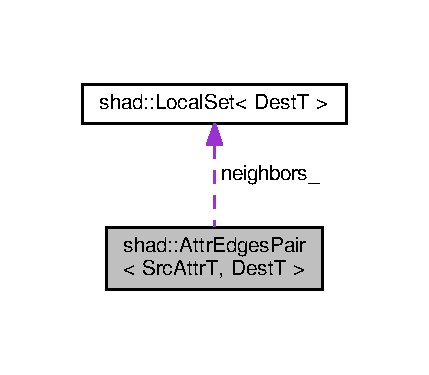
\includegraphics[width=206pt]{classshad_1_1AttrEdgesPair__coll__graph}
\end{center}
\end{figure}
\subsection*{Public Member Functions}
\begin{DoxyCompactItemize}
\item 
size\-\_\-t \hyperlink{classshad_1_1AttrEdgesPair_a9e599e9cd0f48c8f43f601ff2964c518}{Size} ()
\item 
void \hyperlink{classshad_1_1AttrEdgesPair_afa9b9a09795c87ca9c9cc345ddad917e}{Erase} (const Dest\-T \&dest)
\item 
void \hyperlink{classshad_1_1AttrEdgesPair_af51bbca5c672249e3d4365fe56504880}{Async\-Erase} (\hyperlink{classshad_1_1rt_1_1Handle}{rt\-::\-Handle} \&handle, const Dest\-T \&dest)
\item 
void \hyperlink{classshad_1_1AttrEdgesPair_aeec4a60aa7a4b93b62ff8f38774e6709}{Insert} (const Dest\-T \&dest)
\item 
void \hyperlink{classshad_1_1AttrEdgesPair_a1f9ee442c101737b9ceb03c74e4ea78a}{Async\-Insert} (\hyperlink{classshad_1_1rt_1_1Handle}{rt\-::\-Handle} \&handle, const Dest\-T \&dest)
\item 
{\footnotesize template$<$typename Apply\-Fun\-T , typename... Args$>$ }\\void \hyperlink{classshad_1_1AttrEdgesPair_aa18443674f98afa01f346cd3b84086eb}{For\-Each\-Neighbor} (Apply\-Fun\-T \&\&function, Args \&...args)
\item 
{\footnotesize template$<$typename Apply\-Fun\-T , typename... Args$>$ }\\void \hyperlink{classshad_1_1AttrEdgesPair_ab6c5c1f21f98e09b581e920b37a89325}{Async\-For\-Each\-Neighbor} (\hyperlink{classshad_1_1rt_1_1Handle}{rt\-::\-Handle} \&handle, Apply\-Fun\-T \&\&function, Args \&...args)
\end{DoxyCompactItemize}
\subsection*{Public Attributes}
\begin{DoxyCompactItemize}
\item 
Src\-Attr\-T \hyperlink{classshad_1_1AttrEdgesPair_a6296cb2ead29362d2a52f3c5ccef58a1}{attributes\-\_\-}
\item 
\hyperlink{classshad_1_1LocalSet}{Local\-Set}$<$ Dest\-T $>$ \hyperlink{classshad_1_1AttrEdgesPair_a2c1c5d3fac6714fdbff5d0edabf0b334}{neighbors\-\_\-}
\end{DoxyCompactItemize}


\subsection{Member Function Documentation}
\hypertarget{classshad_1_1AttrEdgesPair_af51bbca5c672249e3d4365fe56504880}{\index{shad\-::\-Attr\-Edges\-Pair@{shad\-::\-Attr\-Edges\-Pair}!Async\-Erase@{Async\-Erase}}
\index{Async\-Erase@{Async\-Erase}!shad::AttrEdgesPair@{shad\-::\-Attr\-Edges\-Pair}}
\subsubsection[{Async\-Erase}]{\setlength{\rightskip}{0pt plus 5cm}template$<$typename Src\-Attr\-T , typename Dest\-T $>$ void {\bf shad\-::\-Attr\-Edges\-Pair}$<$ Src\-Attr\-T, Dest\-T $>$\-::Async\-Erase (
\begin{DoxyParamCaption}
\item[{{\bf rt\-::\-Handle} \&}]{handle, }
\item[{const Dest\-T \&}]{dest}
\end{DoxyParamCaption}
)\hspace{0.3cm}{\ttfamily [inline]}}}\label{classshad_1_1AttrEdgesPair_af51bbca5c672249e3d4365fe56504880}
\hypertarget{classshad_1_1AttrEdgesPair_ab6c5c1f21f98e09b581e920b37a89325}{\index{shad\-::\-Attr\-Edges\-Pair@{shad\-::\-Attr\-Edges\-Pair}!Async\-For\-Each\-Neighbor@{Async\-For\-Each\-Neighbor}}
\index{Async\-For\-Each\-Neighbor@{Async\-For\-Each\-Neighbor}!shad::AttrEdgesPair@{shad\-::\-Attr\-Edges\-Pair}}
\subsubsection[{Async\-For\-Each\-Neighbor}]{\setlength{\rightskip}{0pt plus 5cm}template$<$typename Src\-Attr\-T , typename Dest\-T $>$ template$<$typename Apply\-Fun\-T , typename... Args$>$ void {\bf shad\-::\-Attr\-Edges\-Pair}$<$ Src\-Attr\-T, Dest\-T $>$\-::Async\-For\-Each\-Neighbor (
\begin{DoxyParamCaption}
\item[{{\bf rt\-::\-Handle} \&}]{handle, }
\item[{Apply\-Fun\-T \&\&}]{function, }
\item[{Args \&...}]{args}
\end{DoxyParamCaption}
)\hspace{0.3cm}{\ttfamily [inline]}}}\label{classshad_1_1AttrEdgesPair_ab6c5c1f21f98e09b581e920b37a89325}
\hypertarget{classshad_1_1AttrEdgesPair_a1f9ee442c101737b9ceb03c74e4ea78a}{\index{shad\-::\-Attr\-Edges\-Pair@{shad\-::\-Attr\-Edges\-Pair}!Async\-Insert@{Async\-Insert}}
\index{Async\-Insert@{Async\-Insert}!shad::AttrEdgesPair@{shad\-::\-Attr\-Edges\-Pair}}
\subsubsection[{Async\-Insert}]{\setlength{\rightskip}{0pt plus 5cm}template$<$typename Src\-Attr\-T , typename Dest\-T $>$ void {\bf shad\-::\-Attr\-Edges\-Pair}$<$ Src\-Attr\-T, Dest\-T $>$\-::Async\-Insert (
\begin{DoxyParamCaption}
\item[{{\bf rt\-::\-Handle} \&}]{handle, }
\item[{const Dest\-T \&}]{dest}
\end{DoxyParamCaption}
)\hspace{0.3cm}{\ttfamily [inline]}}}\label{classshad_1_1AttrEdgesPair_a1f9ee442c101737b9ceb03c74e4ea78a}
\hypertarget{classshad_1_1AttrEdgesPair_afa9b9a09795c87ca9c9cc345ddad917e}{\index{shad\-::\-Attr\-Edges\-Pair@{shad\-::\-Attr\-Edges\-Pair}!Erase@{Erase}}
\index{Erase@{Erase}!shad::AttrEdgesPair@{shad\-::\-Attr\-Edges\-Pair}}
\subsubsection[{Erase}]{\setlength{\rightskip}{0pt plus 5cm}template$<$typename Src\-Attr\-T , typename Dest\-T $>$ void {\bf shad\-::\-Attr\-Edges\-Pair}$<$ Src\-Attr\-T, Dest\-T $>$\-::Erase (
\begin{DoxyParamCaption}
\item[{const Dest\-T \&}]{dest}
\end{DoxyParamCaption}
)\hspace{0.3cm}{\ttfamily [inline]}}}\label{classshad_1_1AttrEdgesPair_afa9b9a09795c87ca9c9cc345ddad917e}
\hypertarget{classshad_1_1AttrEdgesPair_aa18443674f98afa01f346cd3b84086eb}{\index{shad\-::\-Attr\-Edges\-Pair@{shad\-::\-Attr\-Edges\-Pair}!For\-Each\-Neighbor@{For\-Each\-Neighbor}}
\index{For\-Each\-Neighbor@{For\-Each\-Neighbor}!shad::AttrEdgesPair@{shad\-::\-Attr\-Edges\-Pair}}
\subsubsection[{For\-Each\-Neighbor}]{\setlength{\rightskip}{0pt plus 5cm}template$<$typename Src\-Attr\-T , typename Dest\-T $>$ template$<$typename Apply\-Fun\-T , typename... Args$>$ void {\bf shad\-::\-Attr\-Edges\-Pair}$<$ Src\-Attr\-T, Dest\-T $>$\-::For\-Each\-Neighbor (
\begin{DoxyParamCaption}
\item[{Apply\-Fun\-T \&\&}]{function, }
\item[{Args \&...}]{args}
\end{DoxyParamCaption}
)\hspace{0.3cm}{\ttfamily [inline]}}}\label{classshad_1_1AttrEdgesPair_aa18443674f98afa01f346cd3b84086eb}
\hypertarget{classshad_1_1AttrEdgesPair_aeec4a60aa7a4b93b62ff8f38774e6709}{\index{shad\-::\-Attr\-Edges\-Pair@{shad\-::\-Attr\-Edges\-Pair}!Insert@{Insert}}
\index{Insert@{Insert}!shad::AttrEdgesPair@{shad\-::\-Attr\-Edges\-Pair}}
\subsubsection[{Insert}]{\setlength{\rightskip}{0pt plus 5cm}template$<$typename Src\-Attr\-T , typename Dest\-T $>$ void {\bf shad\-::\-Attr\-Edges\-Pair}$<$ Src\-Attr\-T, Dest\-T $>$\-::Insert (
\begin{DoxyParamCaption}
\item[{const Dest\-T \&}]{dest}
\end{DoxyParamCaption}
)\hspace{0.3cm}{\ttfamily [inline]}}}\label{classshad_1_1AttrEdgesPair_aeec4a60aa7a4b93b62ff8f38774e6709}
\hypertarget{classshad_1_1AttrEdgesPair_a9e599e9cd0f48c8f43f601ff2964c518}{\index{shad\-::\-Attr\-Edges\-Pair@{shad\-::\-Attr\-Edges\-Pair}!Size@{Size}}
\index{Size@{Size}!shad::AttrEdgesPair@{shad\-::\-Attr\-Edges\-Pair}}
\subsubsection[{Size}]{\setlength{\rightskip}{0pt plus 5cm}template$<$typename Src\-Attr\-T , typename Dest\-T $>$ size\-\_\-t {\bf shad\-::\-Attr\-Edges\-Pair}$<$ Src\-Attr\-T, Dest\-T $>$\-::Size (
\begin{DoxyParamCaption}
{}
\end{DoxyParamCaption}
)\hspace{0.3cm}{\ttfamily [inline]}}}\label{classshad_1_1AttrEdgesPair_a9e599e9cd0f48c8f43f601ff2964c518}


\subsection{Member Data Documentation}
\hypertarget{classshad_1_1AttrEdgesPair_a6296cb2ead29362d2a52f3c5ccef58a1}{\index{shad\-::\-Attr\-Edges\-Pair@{shad\-::\-Attr\-Edges\-Pair}!attributes\-\_\-@{attributes\-\_\-}}
\index{attributes\-\_\-@{attributes\-\_\-}!shad::AttrEdgesPair@{shad\-::\-Attr\-Edges\-Pair}}
\subsubsection[{attributes\-\_\-}]{\setlength{\rightskip}{0pt plus 5cm}template$<$typename Src\-Attr\-T , typename Dest\-T $>$ Src\-Attr\-T {\bf shad\-::\-Attr\-Edges\-Pair}$<$ Src\-Attr\-T, Dest\-T $>$\-::attributes\-\_\-}}\label{classshad_1_1AttrEdgesPair_a6296cb2ead29362d2a52f3c5ccef58a1}
\hypertarget{classshad_1_1AttrEdgesPair_a2c1c5d3fac6714fdbff5d0edabf0b334}{\index{shad\-::\-Attr\-Edges\-Pair@{shad\-::\-Attr\-Edges\-Pair}!neighbors\-\_\-@{neighbors\-\_\-}}
\index{neighbors\-\_\-@{neighbors\-\_\-}!shad::AttrEdgesPair@{shad\-::\-Attr\-Edges\-Pair}}
\subsubsection[{neighbors\-\_\-}]{\setlength{\rightskip}{0pt plus 5cm}template$<$typename Src\-Attr\-T , typename Dest\-T $>$ {\bf Local\-Set}$<$Dest\-T$>$ {\bf shad\-::\-Attr\-Edges\-Pair}$<$ Src\-Attr\-T, Dest\-T $>$\-::neighbors\-\_\-}}\label{classshad_1_1AttrEdgesPair_a2c1c5d3fac6714fdbff5d0edabf0b334}


The documentation for this class was generated from the following file\-:\begin{DoxyCompactItemize}
\item 
include/shad/extensions/graph\-\_\-library/\hyperlink{attributed__edge__index_8h}{attributed\-\_\-edge\-\_\-index.\-h}\end{DoxyCompactItemize}

\hypertarget{classshad_1_1AttributedEdgeIndexStorage}{\section{shad\-:\-:Attributed\-Edge\-Index\-Storage$<$ Src\-T, Dest\-T, Src\-Attr\-T, Neighbors\-Storage\-T $>$ Class Template Reference}
\label{classshad_1_1AttributedEdgeIndexStorage}\index{shad\-::\-Attributed\-Edge\-Index\-Storage$<$ Src\-T, Dest\-T, Src\-Attr\-T, Neighbors\-Storage\-T $>$@{shad\-::\-Attributed\-Edge\-Index\-Storage$<$ Src\-T, Dest\-T, Src\-Attr\-T, Neighbors\-Storage\-T $>$}}
}


{\ttfamily \#include $<$shad/extensions/graph\-\_\-library/attributed\-\_\-edge\-\_\-index.\-h$>$}



Collaboration diagram for shad\-:\-:Attributed\-Edge\-Index\-Storage$<$ Src\-T, Dest\-T, Src\-Attr\-T, Neighbors\-Storage\-T $>$\-:
\nopagebreak
\begin{figure}[H]
\begin{center}
\leavevmode
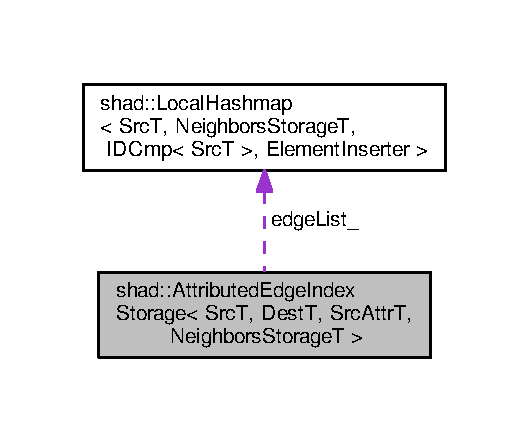
\includegraphics[width=254pt]{classshad_1_1AttributedEdgeIndexStorage__coll__graph}
\end{center}
\end{figure}
\subsection*{Classes}
\begin{DoxyCompactItemize}
\item 
struct \hyperlink{structshad_1_1AttributedEdgeIndexStorage_1_1ElementInserter}{Element\-Inserter}
\item 
struct \hyperlink{structshad_1_1AttributedEdgeIndexStorage_1_1FlatEdgeList}{Flat\-Edge\-List}
\item 
struct \hyperlink{structshad_1_1AttributedEdgeIndexStorage_1_1LocalEdgeListChunk}{Local\-Edge\-List\-Chunk}
\end{DoxyCompactItemize}
\subsection*{Public Types}
\begin{DoxyCompactItemize}
\item 
using \hyperlink{classshad_1_1AttributedEdgeIndexStorage_a9fcd3421b5de8fee1520bb001bae13d5}{Src\-Attributes\-T} = Src\-Attr\-T
\item 
using \hyperlink{classshad_1_1AttributedEdgeIndexStorage_a496b746cebb44b3675c14c22531f6bc5}{Neighbor\-List\-Storage\-T} = Neighbors\-Storage\-T
\item 
using \hyperlink{classshad_1_1AttributedEdgeIndexStorage_ae0e7b167b48bf7a96060a37ae0bb2feb}{Edge\-List\-Storage\-T} = \hyperlink{classshad_1_1LocalHashmap}{Local\-Hashmap}$<$ Src\-T, Neighbors\-Storage\-T, \hyperlink{classshad_1_1IDCmp}{I\-D\-Cmp}$<$ Src\-T $>$, \hyperlink{structshad_1_1AttributedEdgeIndexStorage_1_1ElementInserter}{Element\-Inserter} $>$
\end{DoxyCompactItemize}
\subsection*{Public Member Functions}
\begin{DoxyCompactItemize}
\item 
\hyperlink{classshad_1_1AttributedEdgeIndexStorage_a2206ee347d430507dc8b761932b111ed}{Attributed\-Edge\-Index\-Storage} (const size\-\_\-t num\-Vertices)
\item 
\hyperlink{classshad_1_1AttributedEdgeIndexStorage_a9fcd3421b5de8fee1520bb001bae13d5}{Src\-Attributes\-T} $\ast$ \hyperlink{classshad_1_1AttributedEdgeIndexStorage_ac1d30f94d9a356a98ac6111fa2259693}{Get\-Vertex\-Attributes} (const Src\-T \&src)
\item 
bool \hyperlink{classshad_1_1AttributedEdgeIndexStorage_a2a244b68a0a57f9c082e81360e317ed7}{Get\-Vertex\-Attributes} (const Src\-T \&src, \hyperlink{classshad_1_1AttributedEdgeIndexStorage_a9fcd3421b5de8fee1520bb001bae13d5}{Src\-Attributes\-T} $\ast$attr)
\item 
{\footnotesize template$<$typename Apply\-Fun\-T , typename... Args$>$ }\\void \hyperlink{classshad_1_1AttributedEdgeIndexStorage_a4e7361c272f54f2538e174fccfe25a5d}{Vertex\-Attributes\-Apply} (const Src\-T \&src, Apply\-Fun\-T \&\&function, Args \&...args)
\end{DoxyCompactItemize}
\subsection*{Static Public Member Functions}
\begin{DoxyCompactItemize}
\item 
{\footnotesize template$<$typename Apply\-Fun\-T , typename... Args, std\-::size\-\_\-t... is$>$ }\\static void \hyperlink{classshad_1_1AttributedEdgeIndexStorage_a7bca59f814fc8a2a78d99247c18466f6}{Call\-Vertex\-Attributes\-Apply\-Fun} (\hyperlink{classshad_1_1AttributedEdgeIndexStorage}{Attributed\-Edge\-Index\-Storage}$<$ Src\-T, Dest\-T, Src\-Attr\-T, \hyperlink{classshad_1_1AttributedEdgeIndexStorage_a496b746cebb44b3675c14c22531f6bc5}{Neighbor\-List\-Storage\-T} $>$ $\ast$st\-Ptr, const Src\-T \&src, Apply\-Fun\-T function, std\-::tuple$<$ Args...$>$ \&args, std\-::index\-\_\-sequence$<$ is...$>$)
\end{DoxyCompactItemize}
\subsection*{Public Attributes}
\begin{DoxyCompactItemize}
\item 
\hyperlink{classshad_1_1AttributedEdgeIndexStorage_ae0e7b167b48bf7a96060a37ae0bb2feb}{Edge\-List\-Storage\-T} \hyperlink{classshad_1_1AttributedEdgeIndexStorage_a9b75c33790c1e4fc755dba28371fbe7b}{edge\-List\-\_\-}
\end{DoxyCompactItemize}
\subsection*{Static Public Attributes}
\begin{DoxyCompactItemize}
\item 
static constexpr size\-\_\-t \hyperlink{classshad_1_1AttributedEdgeIndexStorage_a25f1c4ea3b8065bccaa587576d29e262}{k\-Edge\-List\-Chunk\-Size\-\_\-} = 3072 / sizeof(Dest\-T)
\end{DoxyCompactItemize}


\subsection{Member Typedef Documentation}
\hypertarget{classshad_1_1AttributedEdgeIndexStorage_ae0e7b167b48bf7a96060a37ae0bb2feb}{\index{shad\-::\-Attributed\-Edge\-Index\-Storage@{shad\-::\-Attributed\-Edge\-Index\-Storage}!Edge\-List\-Storage\-T@{Edge\-List\-Storage\-T}}
\index{Edge\-List\-Storage\-T@{Edge\-List\-Storage\-T}!shad::AttributedEdgeIndexStorage@{shad\-::\-Attributed\-Edge\-Index\-Storage}}
\subsubsection[{Edge\-List\-Storage\-T}]{\setlength{\rightskip}{0pt plus 5cm}template$<$typename Src\-T, typename Dest\-T, typename Src\-Attr\-T, typename Neighbors\-Storage\-T = Attr\-Edges\-Pair$<$\-Src\-Attr\-T, Dest\-T$>$$>$ using {\bf shad\-::\-Attributed\-Edge\-Index\-Storage}$<$ Src\-T, Dest\-T, Src\-Attr\-T, Neighbors\-Storage\-T $>$\-::{\bf Edge\-List\-Storage\-T} =  {\bf Local\-Hashmap}$<$Src\-T, Neighbors\-Storage\-T, {\bf I\-D\-Cmp}$<$Src\-T$>$, {\bf Element\-Inserter}$>$}}\label{classshad_1_1AttributedEdgeIndexStorage_ae0e7b167b48bf7a96060a37ae0bb2feb}
\hypertarget{classshad_1_1AttributedEdgeIndexStorage_a496b746cebb44b3675c14c22531f6bc5}{\index{shad\-::\-Attributed\-Edge\-Index\-Storage@{shad\-::\-Attributed\-Edge\-Index\-Storage}!Neighbor\-List\-Storage\-T@{Neighbor\-List\-Storage\-T}}
\index{Neighbor\-List\-Storage\-T@{Neighbor\-List\-Storage\-T}!shad::AttributedEdgeIndexStorage@{shad\-::\-Attributed\-Edge\-Index\-Storage}}
\subsubsection[{Neighbor\-List\-Storage\-T}]{\setlength{\rightskip}{0pt plus 5cm}template$<$typename Src\-T, typename Dest\-T, typename Src\-Attr\-T, typename Neighbors\-Storage\-T = Attr\-Edges\-Pair$<$\-Src\-Attr\-T, Dest\-T$>$$>$ using {\bf shad\-::\-Attributed\-Edge\-Index\-Storage}$<$ Src\-T, Dest\-T, Src\-Attr\-T, Neighbors\-Storage\-T $>$\-::{\bf Neighbor\-List\-Storage\-T} =  Neighbors\-Storage\-T}}\label{classshad_1_1AttributedEdgeIndexStorage_a496b746cebb44b3675c14c22531f6bc5}
\hypertarget{classshad_1_1AttributedEdgeIndexStorage_a9fcd3421b5de8fee1520bb001bae13d5}{\index{shad\-::\-Attributed\-Edge\-Index\-Storage@{shad\-::\-Attributed\-Edge\-Index\-Storage}!Src\-Attributes\-T@{Src\-Attributes\-T}}
\index{Src\-Attributes\-T@{Src\-Attributes\-T}!shad::AttributedEdgeIndexStorage@{shad\-::\-Attributed\-Edge\-Index\-Storage}}
\subsubsection[{Src\-Attributes\-T}]{\setlength{\rightskip}{0pt plus 5cm}template$<$typename Src\-T, typename Dest\-T, typename Src\-Attr\-T, typename Neighbors\-Storage\-T = Attr\-Edges\-Pair$<$\-Src\-Attr\-T, Dest\-T$>$$>$ using {\bf shad\-::\-Attributed\-Edge\-Index\-Storage}$<$ Src\-T, Dest\-T, Src\-Attr\-T, Neighbors\-Storage\-T $>$\-::{\bf Src\-Attributes\-T} =  Src\-Attr\-T}}\label{classshad_1_1AttributedEdgeIndexStorage_a9fcd3421b5de8fee1520bb001bae13d5}


\subsection{Constructor \& Destructor Documentation}
\hypertarget{classshad_1_1AttributedEdgeIndexStorage_a2206ee347d430507dc8b761932b111ed}{\index{shad\-::\-Attributed\-Edge\-Index\-Storage@{shad\-::\-Attributed\-Edge\-Index\-Storage}!Attributed\-Edge\-Index\-Storage@{Attributed\-Edge\-Index\-Storage}}
\index{Attributed\-Edge\-Index\-Storage@{Attributed\-Edge\-Index\-Storage}!shad::AttributedEdgeIndexStorage@{shad\-::\-Attributed\-Edge\-Index\-Storage}}
\subsubsection[{Attributed\-Edge\-Index\-Storage}]{\setlength{\rightskip}{0pt plus 5cm}template$<$typename Src\-T, typename Dest\-T, typename Src\-Attr\-T, typename Neighbors\-Storage\-T = Attr\-Edges\-Pair$<$\-Src\-Attr\-T, Dest\-T$>$$>$ {\bf shad\-::\-Attributed\-Edge\-Index\-Storage}$<$ Src\-T, Dest\-T, Src\-Attr\-T, Neighbors\-Storage\-T $>$\-::{\bf Attributed\-Edge\-Index\-Storage} (
\begin{DoxyParamCaption}
\item[{const size\-\_\-t}]{num\-Vertices}
\end{DoxyParamCaption}
)\hspace{0.3cm}{\ttfamily [inline]}, {\ttfamily [explicit]}}}\label{classshad_1_1AttributedEdgeIndexStorage_a2206ee347d430507dc8b761932b111ed}


\subsection{Member Function Documentation}
\hypertarget{classshad_1_1AttributedEdgeIndexStorage_a7bca59f814fc8a2a78d99247c18466f6}{\index{shad\-::\-Attributed\-Edge\-Index\-Storage@{shad\-::\-Attributed\-Edge\-Index\-Storage}!Call\-Vertex\-Attributes\-Apply\-Fun@{Call\-Vertex\-Attributes\-Apply\-Fun}}
\index{Call\-Vertex\-Attributes\-Apply\-Fun@{Call\-Vertex\-Attributes\-Apply\-Fun}!shad::AttributedEdgeIndexStorage@{shad\-::\-Attributed\-Edge\-Index\-Storage}}
\subsubsection[{Call\-Vertex\-Attributes\-Apply\-Fun}]{\setlength{\rightskip}{0pt plus 5cm}template$<$typename Src\-T, typename Dest\-T, typename Src\-Attr\-T, typename Neighbors\-Storage\-T = Attr\-Edges\-Pair$<$\-Src\-Attr\-T, Dest\-T$>$$>$ template$<$typename Apply\-Fun\-T , typename... Args, std\-::size\-\_\-t... is$>$ static void {\bf shad\-::\-Attributed\-Edge\-Index\-Storage}$<$ Src\-T, Dest\-T, Src\-Attr\-T, Neighbors\-Storage\-T $>$\-::Call\-Vertex\-Attributes\-Apply\-Fun (
\begin{DoxyParamCaption}
\item[{{\bf Attributed\-Edge\-Index\-Storage}$<$ Src\-T, Dest\-T, Src\-Attr\-T, {\bf Neighbor\-List\-Storage\-T} $>$ $\ast$}]{st\-Ptr, }
\item[{const Src\-T \&}]{src, }
\item[{Apply\-Fun\-T}]{function, }
\item[{std\-::tuple$<$ Args...$>$ \&}]{args, }
\item[{std\-::index\-\_\-sequence$<$ is...$>$}]{}
\end{DoxyParamCaption}
)\hspace{0.3cm}{\ttfamily [inline]}, {\ttfamily [static]}}}\label{classshad_1_1AttributedEdgeIndexStorage_a7bca59f814fc8a2a78d99247c18466f6}
\hypertarget{classshad_1_1AttributedEdgeIndexStorage_ac1d30f94d9a356a98ac6111fa2259693}{\index{shad\-::\-Attributed\-Edge\-Index\-Storage@{shad\-::\-Attributed\-Edge\-Index\-Storage}!Get\-Vertex\-Attributes@{Get\-Vertex\-Attributes}}
\index{Get\-Vertex\-Attributes@{Get\-Vertex\-Attributes}!shad::AttributedEdgeIndexStorage@{shad\-::\-Attributed\-Edge\-Index\-Storage}}
\subsubsection[{Get\-Vertex\-Attributes}]{\setlength{\rightskip}{0pt plus 5cm}template$<$typename Src\-T, typename Dest\-T, typename Src\-Attr\-T, typename Neighbors\-Storage\-T = Attr\-Edges\-Pair$<$\-Src\-Attr\-T, Dest\-T$>$$>$ {\bf Src\-Attributes\-T}$\ast$ {\bf shad\-::\-Attributed\-Edge\-Index\-Storage}$<$ Src\-T, Dest\-T, Src\-Attr\-T, Neighbors\-Storage\-T $>$\-::Get\-Vertex\-Attributes (
\begin{DoxyParamCaption}
\item[{const Src\-T \&}]{src}
\end{DoxyParamCaption}
)\hspace{0.3cm}{\ttfamily [inline]}}}\label{classshad_1_1AttributedEdgeIndexStorage_ac1d30f94d9a356a98ac6111fa2259693}
\hypertarget{classshad_1_1AttributedEdgeIndexStorage_a2a244b68a0a57f9c082e81360e317ed7}{\index{shad\-::\-Attributed\-Edge\-Index\-Storage@{shad\-::\-Attributed\-Edge\-Index\-Storage}!Get\-Vertex\-Attributes@{Get\-Vertex\-Attributes}}
\index{Get\-Vertex\-Attributes@{Get\-Vertex\-Attributes}!shad::AttributedEdgeIndexStorage@{shad\-::\-Attributed\-Edge\-Index\-Storage}}
\subsubsection[{Get\-Vertex\-Attributes}]{\setlength{\rightskip}{0pt plus 5cm}template$<$typename Src\-T, typename Dest\-T, typename Src\-Attr\-T, typename Neighbors\-Storage\-T = Attr\-Edges\-Pair$<$\-Src\-Attr\-T, Dest\-T$>$$>$ bool {\bf shad\-::\-Attributed\-Edge\-Index\-Storage}$<$ Src\-T, Dest\-T, Src\-Attr\-T, Neighbors\-Storage\-T $>$\-::Get\-Vertex\-Attributes (
\begin{DoxyParamCaption}
\item[{const Src\-T \&}]{src, }
\item[{{\bf Src\-Attributes\-T} $\ast$}]{attr}
\end{DoxyParamCaption}
)\hspace{0.3cm}{\ttfamily [inline]}}}\label{classshad_1_1AttributedEdgeIndexStorage_a2a244b68a0a57f9c082e81360e317ed7}
\hypertarget{classshad_1_1AttributedEdgeIndexStorage_a4e7361c272f54f2538e174fccfe25a5d}{\index{shad\-::\-Attributed\-Edge\-Index\-Storage@{shad\-::\-Attributed\-Edge\-Index\-Storage}!Vertex\-Attributes\-Apply@{Vertex\-Attributes\-Apply}}
\index{Vertex\-Attributes\-Apply@{Vertex\-Attributes\-Apply}!shad::AttributedEdgeIndexStorage@{shad\-::\-Attributed\-Edge\-Index\-Storage}}
\subsubsection[{Vertex\-Attributes\-Apply}]{\setlength{\rightskip}{0pt plus 5cm}template$<$typename Src\-T, typename Dest\-T, typename Src\-Attr\-T, typename Neighbors\-Storage\-T = Attr\-Edges\-Pair$<$\-Src\-Attr\-T, Dest\-T$>$$>$ template$<$typename Apply\-Fun\-T , typename... Args$>$ void {\bf shad\-::\-Attributed\-Edge\-Index\-Storage}$<$ Src\-T, Dest\-T, Src\-Attr\-T, Neighbors\-Storage\-T $>$\-::Vertex\-Attributes\-Apply (
\begin{DoxyParamCaption}
\item[{const Src\-T \&}]{src, }
\item[{Apply\-Fun\-T \&\&}]{function, }
\item[{Args \&...}]{args}
\end{DoxyParamCaption}
)\hspace{0.3cm}{\ttfamily [inline]}}}\label{classshad_1_1AttributedEdgeIndexStorage_a4e7361c272f54f2538e174fccfe25a5d}


\subsection{Member Data Documentation}
\hypertarget{classshad_1_1AttributedEdgeIndexStorage_a9b75c33790c1e4fc755dba28371fbe7b}{\index{shad\-::\-Attributed\-Edge\-Index\-Storage@{shad\-::\-Attributed\-Edge\-Index\-Storage}!edge\-List\-\_\-@{edge\-List\-\_\-}}
\index{edge\-List\-\_\-@{edge\-List\-\_\-}!shad::AttributedEdgeIndexStorage@{shad\-::\-Attributed\-Edge\-Index\-Storage}}
\subsubsection[{edge\-List\-\_\-}]{\setlength{\rightskip}{0pt plus 5cm}template$<$typename Src\-T, typename Dest\-T, typename Src\-Attr\-T, typename Neighbors\-Storage\-T = Attr\-Edges\-Pair$<$\-Src\-Attr\-T, Dest\-T$>$$>$ {\bf Edge\-List\-Storage\-T} {\bf shad\-::\-Attributed\-Edge\-Index\-Storage}$<$ Src\-T, Dest\-T, Src\-Attr\-T, Neighbors\-Storage\-T $>$\-::edge\-List\-\_\-}}\label{classshad_1_1AttributedEdgeIndexStorage_a9b75c33790c1e4fc755dba28371fbe7b}
\hypertarget{classshad_1_1AttributedEdgeIndexStorage_a25f1c4ea3b8065bccaa587576d29e262}{\index{shad\-::\-Attributed\-Edge\-Index\-Storage@{shad\-::\-Attributed\-Edge\-Index\-Storage}!k\-Edge\-List\-Chunk\-Size\-\_\-@{k\-Edge\-List\-Chunk\-Size\-\_\-}}
\index{k\-Edge\-List\-Chunk\-Size\-\_\-@{k\-Edge\-List\-Chunk\-Size\-\_\-}!shad::AttributedEdgeIndexStorage@{shad\-::\-Attributed\-Edge\-Index\-Storage}}
\subsubsection[{k\-Edge\-List\-Chunk\-Size\-\_\-}]{\setlength{\rightskip}{0pt plus 5cm}template$<$typename Src\-T, typename Dest\-T, typename Src\-Attr\-T, typename Neighbors\-Storage\-T = Attr\-Edges\-Pair$<$\-Src\-Attr\-T, Dest\-T$>$$>$ constexpr size\-\_\-t {\bf shad\-::\-Attributed\-Edge\-Index\-Storage}$<$ Src\-T, Dest\-T, Src\-Attr\-T, Neighbors\-Storage\-T $>$\-::k\-Edge\-List\-Chunk\-Size\-\_\- = 3072 / sizeof(Dest\-T)\hspace{0.3cm}{\ttfamily [static]}}}\label{classshad_1_1AttributedEdgeIndexStorage_a25f1c4ea3b8065bccaa587576d29e262}


The documentation for this class was generated from the following file\-:\begin{DoxyCompactItemize}
\item 
include/shad/extensions/graph\-\_\-library/\hyperlink{attributed__edge__index_8h}{attributed\-\_\-edge\-\_\-index.\-h}\end{DoxyCompactItemize}

\hypertarget{classshad_1_1buffered__insert__iterator}{\section{shad\-:\-:buffered\-\_\-insert\-\_\-iterator$<$ Container $>$ Class Template Reference}
\label{classshad_1_1buffered__insert__iterator}\index{shad\-::buffered\-\_\-insert\-\_\-iterator$<$ Container $>$@{shad\-::buffered\-\_\-insert\-\_\-iterator$<$ Container $>$}}
}


Buffered insert iterator.  




{\ttfamily \#include $<$shad/core/iterator.\-h$>$}



Inheritance diagram for shad\-:\-:buffered\-\_\-insert\-\_\-iterator$<$ Container $>$\-:
\nopagebreak
\begin{figure}[H]
\begin{center}
\leavevmode
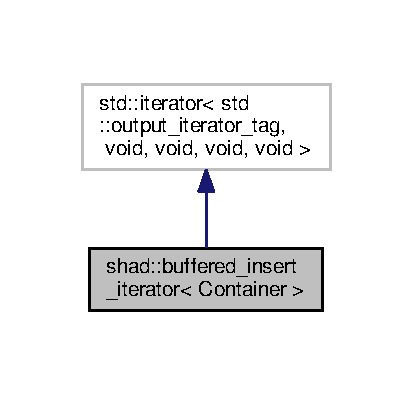
\includegraphics[width=198pt]{classshad_1_1buffered__insert__iterator__inherit__graph}
\end{center}
\end{figure}


Collaboration diagram for shad\-:\-:buffered\-\_\-insert\-\_\-iterator$<$ Container $>$\-:
\nopagebreak
\begin{figure}[H]
\begin{center}
\leavevmode
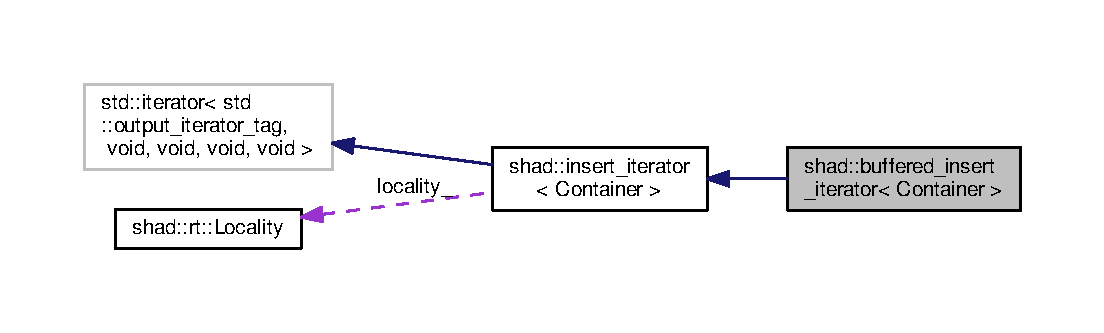
\includegraphics[width=198pt]{classshad_1_1buffered__insert__iterator__coll__graph}
\end{center}
\end{figure}
\subsection*{Public Types}
\begin{DoxyCompactItemize}
\item 
using \hyperlink{classshad_1_1buffered__insert__iterator_a8d1e5c22ad001becf13b9d0f452eecf2}{container\-\_\-type} = Container
\end{DoxyCompactItemize}
\subsection*{Public Member Functions}
\begin{DoxyCompactItemize}
\item 
\hyperlink{classshad_1_1buffered__insert__iterator_a30c2613f13dc91cfb3f1b37099dc00c5}{buffered\-\_\-insert\-\_\-iterator} (Container \&container, Iterator iterator)
\begin{DoxyCompactList}\small\item\em Constructor. \end{DoxyCompactList}\item 
\hyperlink{classshad_1_1buffered__insert__iterator}{buffered\-\_\-insert\-\_\-iterator} \& \hyperlink{classshad_1_1buffered__insert__iterator_ae52408e8adbe5dfd80c6347a3b93d017}{operator=} (const value\-\_\-type \&value)
\begin{DoxyCompactList}\small\item\em The assignment operator. \end{DoxyCompactList}\item 
void \hyperlink{classshad_1_1buffered__insert__iterator_aadf229f6aac3dbdfc204b7f6309b2e71}{flush} ()
\begin{DoxyCompactList}\small\item\em Flushes pending insertions to the container. \end{DoxyCompactList}\item 
\hyperlink{classshad_1_1buffered__insert__iterator_ae375c7de831143a927f581b441aa987d}{$\sim$buffered\-\_\-insert\-\_\-iterator} ()
\begin{DoxyCompactList}\small\item\em Destructor. \end{DoxyCompactList}\item 
\hyperlink{classshad_1_1buffered__insert__iterator}{buffered\-\_\-insert\-\_\-iterator} \& \hyperlink{classshad_1_1buffered__insert__iterator_a329d91c1c95a1d86fe9b3cd14032bc23}{operator$\ast$} ()
\item 
\hyperlink{classshad_1_1buffered__insert__iterator}{buffered\-\_\-insert\-\_\-iterator} \& \hyperlink{classshad_1_1buffered__insert__iterator_a270b0bd4c6bfaa0cf656c4e65c676bef}{operator++} ()
\item 
\hyperlink{classshad_1_1buffered__insert__iterator}{buffered\-\_\-insert\-\_\-iterator} \& \hyperlink{classshad_1_1buffered__insert__iterator_a326909f8fb18bdb6ae9744e3b4a189f7}{operator++} (int)
\end{DoxyCompactItemize}
\subsection*{Protected Attributes}
\begin{DoxyCompactItemize}
\item 
Container $\ast$ \hyperlink{classshad_1_1buffered__insert__iterator_a9503b8887e7d8c9a911293c96898007c}{container\-\_\-}
\item 
Iterator \hyperlink{classshad_1_1buffered__insert__iterator_a47e9e89830c5acbda85c3d6a43cc6713}{iterator\-\_\-}
\end{DoxyCompactItemize}


\subsection{Detailed Description}
\subsubsection*{template$<$typename Container$>$class shad\-::buffered\-\_\-insert\-\_\-iterator$<$ Container $>$}

Buffered insert iterator. 

\hyperlink{classshad_1_1buffered__insert__iterator}{shad\-::buffered\-\_\-insert\-\_\-iterator} is an Output\-Iterator that inserts elements into a distributed container for which it was constructed, at the position pointed to by the supplied iterator. The buffered insertion is performed whenever the iterator (whether dereferenced or not) is assigned to. The buffer to be flushed into the container when the \hyperlink{classshad_1_1buffered__insert__iterator_aadf229f6aac3dbdfc204b7f6309b2e71}{flush()} function is called and also upon destruction. Incrementing the \hyperlink{classshad_1_1buffered__insert__iterator}{shad\-::buffered\-\_\-insert\-\_\-iterator} is a no-\/op.


\begin{DoxyTemplParams}{Template Parameters}
{\em Container} & The type of the distributed container. \\
\hline
\end{DoxyTemplParams}


\subsection{Member Typedef Documentation}
\hypertarget{classshad_1_1buffered__insert__iterator_a8d1e5c22ad001becf13b9d0f452eecf2}{\index{shad\-::buffered\-\_\-insert\-\_\-iterator@{shad\-::buffered\-\_\-insert\-\_\-iterator}!container\-\_\-type@{container\-\_\-type}}
\index{container\-\_\-type@{container\-\_\-type}!shad::buffered_insert_iterator@{shad\-::buffered\-\_\-insert\-\_\-iterator}}
\subsubsection[{container\-\_\-type}]{\setlength{\rightskip}{0pt plus 5cm}template$<$typename Container $>$ using {\bf shad\-::buffered\-\_\-insert\-\_\-iterator}$<$ Container $>$\-::{\bf container\-\_\-type} =  Container}}\label{classshad_1_1buffered__insert__iterator_a8d1e5c22ad001becf13b9d0f452eecf2}


\subsection{Constructor \& Destructor Documentation}
\hypertarget{classshad_1_1buffered__insert__iterator_a30c2613f13dc91cfb3f1b37099dc00c5}{\index{shad\-::buffered\-\_\-insert\-\_\-iterator@{shad\-::buffered\-\_\-insert\-\_\-iterator}!buffered\-\_\-insert\-\_\-iterator@{buffered\-\_\-insert\-\_\-iterator}}
\index{buffered\-\_\-insert\-\_\-iterator@{buffered\-\_\-insert\-\_\-iterator}!shad::buffered_insert_iterator@{shad\-::buffered\-\_\-insert\-\_\-iterator}}
\subsubsection[{buffered\-\_\-insert\-\_\-iterator}]{\setlength{\rightskip}{0pt plus 5cm}template$<$typename Container $>$ {\bf shad\-::buffered\-\_\-insert\-\_\-iterator}$<$ Container $>$\-::{\bf buffered\-\_\-insert\-\_\-iterator} (
\begin{DoxyParamCaption}
\item[{Container \&}]{container, }
\item[{Iterator}]{iterator}
\end{DoxyParamCaption}
)\hspace{0.3cm}{\ttfamily [inline]}}}\label{classshad_1_1buffered__insert__iterator_a30c2613f13dc91cfb3f1b37099dc00c5}


Constructor. 


\begin{DoxyParams}{Parameters}
{\em container} & The container into which the iterator inserts. \\
\hline
{\em iterator} & The position at which the iterator starts to insert. \\
\hline
\end{DoxyParams}
\hypertarget{classshad_1_1buffered__insert__iterator_ae375c7de831143a927f581b441aa987d}{\index{shad\-::buffered\-\_\-insert\-\_\-iterator@{shad\-::buffered\-\_\-insert\-\_\-iterator}!$\sim$buffered\-\_\-insert\-\_\-iterator@{$\sim$buffered\-\_\-insert\-\_\-iterator}}
\index{$\sim$buffered\-\_\-insert\-\_\-iterator@{$\sim$buffered\-\_\-insert\-\_\-iterator}!shad::buffered_insert_iterator@{shad\-::buffered\-\_\-insert\-\_\-iterator}}
\subsubsection[{$\sim$buffered\-\_\-insert\-\_\-iterator}]{\setlength{\rightskip}{0pt plus 5cm}template$<$typename Container $>$ {\bf shad\-::buffered\-\_\-insert\-\_\-iterator}$<$ Container $>$\-::$\sim${\bf buffered\-\_\-insert\-\_\-iterator} (
\begin{DoxyParamCaption}
{}
\end{DoxyParamCaption}
)\hspace{0.3cm}{\ttfamily [inline]}}}\label{classshad_1_1buffered__insert__iterator_ae375c7de831143a927f581b441aa987d}


Destructor. 

The destruction flushes all pending insertions into the container. 

\subsection{Member Function Documentation}
\hypertarget{classshad_1_1buffered__insert__iterator_aadf229f6aac3dbdfc204b7f6309b2e71}{\index{shad\-::buffered\-\_\-insert\-\_\-iterator@{shad\-::buffered\-\_\-insert\-\_\-iterator}!flush@{flush}}
\index{flush@{flush}!shad::buffered_insert_iterator@{shad\-::buffered\-\_\-insert\-\_\-iterator}}
\subsubsection[{flush}]{\setlength{\rightskip}{0pt plus 5cm}template$<$typename Container $>$ void {\bf shad\-::buffered\-\_\-insert\-\_\-iterator}$<$ Container $>$\-::flush (
\begin{DoxyParamCaption}
{}
\end{DoxyParamCaption}
)\hspace{0.3cm}{\ttfamily [inline]}}}\label{classshad_1_1buffered__insert__iterator_aadf229f6aac3dbdfc204b7f6309b2e71}


Flushes pending insertions to the container. 

\hypertarget{classshad_1_1buffered__insert__iterator_a329d91c1c95a1d86fe9b3cd14032bc23}{\index{shad\-::buffered\-\_\-insert\-\_\-iterator@{shad\-::buffered\-\_\-insert\-\_\-iterator}!operator$\ast$@{operator$\ast$}}
\index{operator$\ast$@{operator$\ast$}!shad::buffered_insert_iterator@{shad\-::buffered\-\_\-insert\-\_\-iterator}}
\subsubsection[{operator$\ast$}]{\setlength{\rightskip}{0pt plus 5cm}template$<$typename Container $>$ {\bf buffered\-\_\-insert\-\_\-iterator}\& {\bf shad\-::buffered\-\_\-insert\-\_\-iterator}$<$ Container $>$\-::operator$\ast$ (
\begin{DoxyParamCaption}
{}
\end{DoxyParamCaption}
)\hspace{0.3cm}{\ttfamily [inline]}}}\label{classshad_1_1buffered__insert__iterator_a329d91c1c95a1d86fe9b3cd14032bc23}
\hypertarget{classshad_1_1buffered__insert__iterator_a270b0bd4c6bfaa0cf656c4e65c676bef}{\index{shad\-::buffered\-\_\-insert\-\_\-iterator@{shad\-::buffered\-\_\-insert\-\_\-iterator}!operator++@{operator++}}
\index{operator++@{operator++}!shad::buffered_insert_iterator@{shad\-::buffered\-\_\-insert\-\_\-iterator}}
\subsubsection[{operator++}]{\setlength{\rightskip}{0pt plus 5cm}template$<$typename Container $>$ {\bf buffered\-\_\-insert\-\_\-iterator}\& {\bf shad\-::buffered\-\_\-insert\-\_\-iterator}$<$ Container $>$\-::operator++ (
\begin{DoxyParamCaption}
{}
\end{DoxyParamCaption}
)\hspace{0.3cm}{\ttfamily [inline]}}}\label{classshad_1_1buffered__insert__iterator_a270b0bd4c6bfaa0cf656c4e65c676bef}
\hypertarget{classshad_1_1buffered__insert__iterator_a326909f8fb18bdb6ae9744e3b4a189f7}{\index{shad\-::buffered\-\_\-insert\-\_\-iterator@{shad\-::buffered\-\_\-insert\-\_\-iterator}!operator++@{operator++}}
\index{operator++@{operator++}!shad::buffered_insert_iterator@{shad\-::buffered\-\_\-insert\-\_\-iterator}}
\subsubsection[{operator++}]{\setlength{\rightskip}{0pt plus 5cm}template$<$typename Container $>$ {\bf buffered\-\_\-insert\-\_\-iterator}\& {\bf shad\-::buffered\-\_\-insert\-\_\-iterator}$<$ Container $>$\-::operator++ (
\begin{DoxyParamCaption}
\item[{int}]{}
\end{DoxyParamCaption}
)\hspace{0.3cm}{\ttfamily [inline]}}}\label{classshad_1_1buffered__insert__iterator_a326909f8fb18bdb6ae9744e3b4a189f7}
\hypertarget{classshad_1_1buffered__insert__iterator_ae52408e8adbe5dfd80c6347a3b93d017}{\index{shad\-::buffered\-\_\-insert\-\_\-iterator@{shad\-::buffered\-\_\-insert\-\_\-iterator}!operator=@{operator=}}
\index{operator=@{operator=}!shad::buffered_insert_iterator@{shad\-::buffered\-\_\-insert\-\_\-iterator}}
\subsubsection[{operator=}]{\setlength{\rightskip}{0pt plus 5cm}template$<$typename Container $>$ {\bf buffered\-\_\-insert\-\_\-iterator}\& {\bf shad\-::buffered\-\_\-insert\-\_\-iterator}$<$ Container $>$\-::operator= (
\begin{DoxyParamCaption}
\item[{const value\-\_\-type \&}]{value}
\end{DoxyParamCaption}
)\hspace{0.3cm}{\ttfamily [inline]}}}\label{classshad_1_1buffered__insert__iterator_ae52408e8adbe5dfd80c6347a3b93d017}


The assignment operator. 

The assignment operator inserts a value (through buffering) and advance iterator.


\begin{DoxyParams}{Parameters}
{\em value} & A const reference to the value to be inserted.\\
\hline
\end{DoxyParams}
\begin{DoxyReturn}{Returns}
A self reference. 
\end{DoxyReturn}


\subsection{Member Data Documentation}
\hypertarget{classshad_1_1buffered__insert__iterator_a9503b8887e7d8c9a911293c96898007c}{\index{shad\-::buffered\-\_\-insert\-\_\-iterator@{shad\-::buffered\-\_\-insert\-\_\-iterator}!container\-\_\-@{container\-\_\-}}
\index{container\-\_\-@{container\-\_\-}!shad::buffered_insert_iterator@{shad\-::buffered\-\_\-insert\-\_\-iterator}}
\subsubsection[{container\-\_\-}]{\setlength{\rightskip}{0pt plus 5cm}template$<$typename Container $>$ Container$\ast$ {\bf shad\-::buffered\-\_\-insert\-\_\-iterator}$<$ Container $>$\-::container\-\_\-\hspace{0.3cm}{\ttfamily [protected]}}}\label{classshad_1_1buffered__insert__iterator_a9503b8887e7d8c9a911293c96898007c}
\hypertarget{classshad_1_1buffered__insert__iterator_a47e9e89830c5acbda85c3d6a43cc6713}{\index{shad\-::buffered\-\_\-insert\-\_\-iterator@{shad\-::buffered\-\_\-insert\-\_\-iterator}!iterator\-\_\-@{iterator\-\_\-}}
\index{iterator\-\_\-@{iterator\-\_\-}!shad::buffered_insert_iterator@{shad\-::buffered\-\_\-insert\-\_\-iterator}}
\subsubsection[{iterator\-\_\-}]{\setlength{\rightskip}{0pt plus 5cm}template$<$typename Container $>$ Iterator {\bf shad\-::buffered\-\_\-insert\-\_\-iterator}$<$ Container $>$\-::iterator\-\_\-\hspace{0.3cm}{\ttfamily [protected]}}}\label{classshad_1_1buffered__insert__iterator_a47e9e89830c5acbda85c3d6a43cc6713}


The documentation for this class was generated from the following file\-:\begin{DoxyCompactItemize}
\item 
include/shad/core/\hyperlink{iterator_8h}{iterator.\-h}\end{DoxyCompactItemize}

\hypertarget{classshad_1_1AbstractDataStructure_1_1Catalog}{\section{shad\-:\-:Abstract\-Data\-Structure$<$ Data\-Structure $>$\-:\-:Catalog Class Reference}
\label{classshad_1_1AbstractDataStructure_1_1Catalog}\index{shad\-::\-Abstract\-Data\-Structure$<$ Data\-Structure $>$\-::\-Catalog@{shad\-::\-Abstract\-Data\-Structure$<$ Data\-Structure $>$\-::\-Catalog}}
}


{\ttfamily \#include $<$shad/data\-\_\-structures/abstract\-\_\-data\-\_\-structure.\-h$>$}

\subsection*{Public Member Functions}
\begin{DoxyCompactItemize}
\item 
void \hyperlink{classshad_1_1AbstractDataStructure_1_1Catalog_a1e2b195f0047a90bbc375443c7de7e23}{Insert} (const \hyperlink{classshad_1_1AbstractDataStructure_a8772079d2686692828cfbf342cc2b594}{Object\-I\-D} \&oid, const \hyperlink{classshad_1_1AbstractDataStructure_a8bb29450966955c546d40421ce46316f}{Shared\-Ptr} ce)
\item 
void \hyperlink{classshad_1_1AbstractDataStructure_1_1Catalog_a2e551228f9c8b9a7762eb351a11cf99e}{Erase} (const \hyperlink{classshad_1_1AbstractDataStructure_a8772079d2686692828cfbf342cc2b594}{Object\-I\-D} \&oid)
\item 
\hyperlink{classshad_1_1AbstractDataStructure_a8bb29450966955c546d40421ce46316f}{Shared\-Ptr} \hyperlink{classshad_1_1AbstractDataStructure_1_1Catalog_a776520c4f9060fc8c9128ac63e8a3753}{Get\-Ptr} (const \hyperlink{classshad_1_1AbstractDataStructure_a8772079d2686692828cfbf342cc2b594}{Object\-I\-D} \&oid)
\item 
\hyperlink{classshad_1_1AbstractDataStructure_a8772079d2686692828cfbf342cc2b594}{Object\-I\-D} \hyperlink{classshad_1_1AbstractDataStructure_1_1Catalog_a5bf01b25dbb91f77b9b03866dedeb06a}{Get\-Next\-I\-D} ()
\end{DoxyCompactItemize}
\subsection*{Static Public Member Functions}
\begin{DoxyCompactItemize}
\item 
static \hyperlink{classshad_1_1AbstractDataStructure_1_1Catalog}{Catalog} $\ast$ \hyperlink{classshad_1_1AbstractDataStructure_1_1Catalog_a13204d5ff4497f03b438f9cf9ff6253e}{Instance} ()
\end{DoxyCompactItemize}


\subsection{Member Function Documentation}
\hypertarget{classshad_1_1AbstractDataStructure_1_1Catalog_a2e551228f9c8b9a7762eb351a11cf99e}{\index{shad\-::\-Abstract\-Data\-Structure\-::\-Catalog@{shad\-::\-Abstract\-Data\-Structure\-::\-Catalog}!Erase@{Erase}}
\index{Erase@{Erase}!shad::AbstractDataStructure::Catalog@{shad\-::\-Abstract\-Data\-Structure\-::\-Catalog}}
\subsubsection[{Erase}]{\setlength{\rightskip}{0pt plus 5cm}template$<$typename Data\-Structure$>$ void {\bf shad\-::\-Abstract\-Data\-Structure}$<$ Data\-Structure $>$\-::Catalog\-::\-Erase (
\begin{DoxyParamCaption}
\item[{const {\bf Object\-I\-D} \&}]{oid}
\end{DoxyParamCaption}
)\hspace{0.3cm}{\ttfamily [inline]}}}\label{classshad_1_1AbstractDataStructure_1_1Catalog_a2e551228f9c8b9a7762eb351a11cf99e}
\hypertarget{classshad_1_1AbstractDataStructure_1_1Catalog_a5bf01b25dbb91f77b9b03866dedeb06a}{\index{shad\-::\-Abstract\-Data\-Structure\-::\-Catalog@{shad\-::\-Abstract\-Data\-Structure\-::\-Catalog}!Get\-Next\-I\-D@{Get\-Next\-I\-D}}
\index{Get\-Next\-I\-D@{Get\-Next\-I\-D}!shad::AbstractDataStructure::Catalog@{shad\-::\-Abstract\-Data\-Structure\-::\-Catalog}}
\subsubsection[{Get\-Next\-I\-D}]{\setlength{\rightskip}{0pt plus 5cm}template$<$typename Data\-Structure$>$ {\bf Object\-I\-D} {\bf shad\-::\-Abstract\-Data\-Structure}$<$ Data\-Structure $>$\-::Catalog\-::\-Get\-Next\-I\-D (
\begin{DoxyParamCaption}
{}
\end{DoxyParamCaption}
)\hspace{0.3cm}{\ttfamily [inline]}}}\label{classshad_1_1AbstractDataStructure_1_1Catalog_a5bf01b25dbb91f77b9b03866dedeb06a}
\hypertarget{classshad_1_1AbstractDataStructure_1_1Catalog_a776520c4f9060fc8c9128ac63e8a3753}{\index{shad\-::\-Abstract\-Data\-Structure\-::\-Catalog@{shad\-::\-Abstract\-Data\-Structure\-::\-Catalog}!Get\-Ptr@{Get\-Ptr}}
\index{Get\-Ptr@{Get\-Ptr}!shad::AbstractDataStructure::Catalog@{shad\-::\-Abstract\-Data\-Structure\-::\-Catalog}}
\subsubsection[{Get\-Ptr}]{\setlength{\rightskip}{0pt plus 5cm}template$<$typename Data\-Structure$>$ {\bf Shared\-Ptr} {\bf shad\-::\-Abstract\-Data\-Structure}$<$ Data\-Structure $>$\-::Catalog\-::\-Get\-Ptr (
\begin{DoxyParamCaption}
\item[{const {\bf Object\-I\-D} \&}]{oid}
\end{DoxyParamCaption}
)\hspace{0.3cm}{\ttfamily [inline]}}}\label{classshad_1_1AbstractDataStructure_1_1Catalog_a776520c4f9060fc8c9128ac63e8a3753}
\hypertarget{classshad_1_1AbstractDataStructure_1_1Catalog_a1e2b195f0047a90bbc375443c7de7e23}{\index{shad\-::\-Abstract\-Data\-Structure\-::\-Catalog@{shad\-::\-Abstract\-Data\-Structure\-::\-Catalog}!Insert@{Insert}}
\index{Insert@{Insert}!shad::AbstractDataStructure::Catalog@{shad\-::\-Abstract\-Data\-Structure\-::\-Catalog}}
\subsubsection[{Insert}]{\setlength{\rightskip}{0pt plus 5cm}template$<$typename Data\-Structure$>$ void {\bf shad\-::\-Abstract\-Data\-Structure}$<$ Data\-Structure $>$\-::Catalog\-::\-Insert (
\begin{DoxyParamCaption}
\item[{const {\bf Object\-I\-D} \&}]{oid, }
\item[{const {\bf Shared\-Ptr}}]{ce}
\end{DoxyParamCaption}
)\hspace{0.3cm}{\ttfamily [inline]}}}\label{classshad_1_1AbstractDataStructure_1_1Catalog_a1e2b195f0047a90bbc375443c7de7e23}
\hypertarget{classshad_1_1AbstractDataStructure_1_1Catalog_a13204d5ff4497f03b438f9cf9ff6253e}{\index{shad\-::\-Abstract\-Data\-Structure\-::\-Catalog@{shad\-::\-Abstract\-Data\-Structure\-::\-Catalog}!Instance@{Instance}}
\index{Instance@{Instance}!shad::AbstractDataStructure::Catalog@{shad\-::\-Abstract\-Data\-Structure\-::\-Catalog}}
\subsubsection[{Instance}]{\setlength{\rightskip}{0pt plus 5cm}template$<$typename Data\-Structure$>$ static {\bf Catalog}$\ast$ {\bf shad\-::\-Abstract\-Data\-Structure}$<$ Data\-Structure $>$\-::Catalog\-::\-Instance (
\begin{DoxyParamCaption}
{}
\end{DoxyParamCaption}
)\hspace{0.3cm}{\ttfamily [inline]}, {\ttfamily [static]}}}\label{classshad_1_1AbstractDataStructure_1_1Catalog_a13204d5ff4497f03b438f9cf9ff6253e}


The documentation for this class was generated from the following file\-:\begin{DoxyCompactItemize}
\item 
include/shad/data\-\_\-structures/\hyperlink{abstract__data__structure_8h}{abstract\-\_\-data\-\_\-structure.\-h}\end{DoxyCompactItemize}

\hypertarget{classshad_1_1DefaultEdgeIndexStorage}{\section{shad\-:\-:Default\-Edge\-Index\-Storage$<$ Src\-T, Dest\-T, Neighbors\-Storage\-T $>$ Class Template Reference}
\label{classshad_1_1DefaultEdgeIndexStorage}\index{shad\-::\-Default\-Edge\-Index\-Storage$<$ Src\-T, Dest\-T, Neighbors\-Storage\-T $>$@{shad\-::\-Default\-Edge\-Index\-Storage$<$ Src\-T, Dest\-T, Neighbors\-Storage\-T $>$}}
}


{\ttfamily \#include $<$shad/extensions/graph\-\_\-library/local\-\_\-edge\-\_\-index.\-h$>$}



Collaboration diagram for shad\-:\-:Default\-Edge\-Index\-Storage$<$ Src\-T, Dest\-T, Neighbors\-Storage\-T $>$\-:
\nopagebreak
\begin{figure}[H]
\begin{center}
\leavevmode
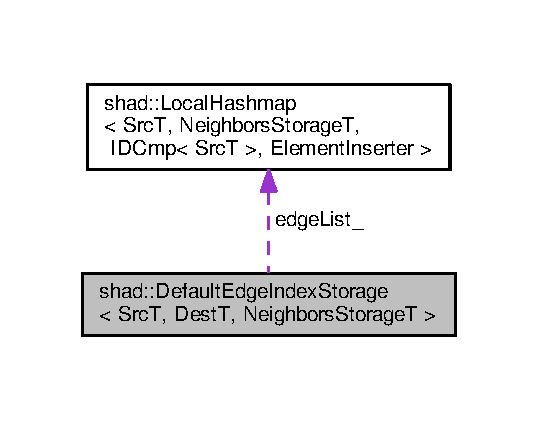
\includegraphics[width=258pt]{classshad_1_1DefaultEdgeIndexStorage__coll__graph}
\end{center}
\end{figure}
\subsection*{Classes}
\begin{DoxyCompactItemize}
\item 
struct \hyperlink{structshad_1_1DefaultEdgeIndexStorage_1_1ElementInserter}{Element\-Inserter}
\item 
struct \hyperlink{structshad_1_1DefaultEdgeIndexStorage_1_1EmptyAttr}{Empty\-Attr}
\item 
struct \hyperlink{structshad_1_1DefaultEdgeIndexStorage_1_1FlatEdgeList}{Flat\-Edge\-List}
\item 
struct \hyperlink{structshad_1_1DefaultEdgeIndexStorage_1_1LocalEdgeListChunk}{Local\-Edge\-List\-Chunk}
\end{DoxyCompactItemize}
\subsection*{Public Types}
\begin{DoxyCompactItemize}
\item 
using \hyperlink{classshad_1_1DefaultEdgeIndexStorage_a70d9110c20e453941e2bfa372463bd92}{Src\-Attributes\-T} = \hyperlink{structshad_1_1DefaultEdgeIndexStorage_1_1EmptyAttr}{Empty\-Attr}
\item 
using \hyperlink{classshad_1_1DefaultEdgeIndexStorage_aae1425fda169243d97fa1e39e4417fa5}{Neighbor\-List\-Storage\-T} = Neighbors\-Storage\-T
\item 
using \hyperlink{classshad_1_1DefaultEdgeIndexStorage_af083de6d56b46413f55dc5fea0384afa}{Edge\-List\-Storage\-T} = \hyperlink{classshad_1_1LocalHashmap}{Local\-Hashmap}$<$ Src\-T, Neighbors\-Storage\-T, \hyperlink{classshad_1_1IDCmp}{I\-D\-Cmp}$<$ Src\-T $>$, \hyperlink{structshad_1_1DefaultEdgeIndexStorage_1_1ElementInserter}{Element\-Inserter} $>$
\end{DoxyCompactItemize}
\subsection*{Public Member Functions}
\begin{DoxyCompactItemize}
\item 
\hyperlink{classshad_1_1DefaultEdgeIndexStorage_a4f75c63f3ebeaf329fd9945204717de6}{Default\-Edge\-Index\-Storage} (const size\-\_\-t num\-Vertices)
\item 
\hyperlink{classshad_1_1DefaultEdgeIndexStorage_a84a6989a03534e76b1d3d32b450ff3b4}{Default\-Edge\-Index\-Storage} (const size\-\_\-t num\-Vertices, const \hyperlink{classshad_1_1DefaultEdgeIndexStorage_a70d9110c20e453941e2bfa372463bd92}{Src\-Attributes\-T} \&)
\item 
{\footnotesize template$<$typename Apply\-Fun\-T , typename... Args$>$ }\\void \hyperlink{classshad_1_1DefaultEdgeIndexStorage_ae5ac6e09a0e97a6af9fb7e6a8a225c06}{For\-Each\-Attributed\-Vertex\-Neighbor} (const Src\-T \&src, Apply\-Fun\-T \&\&function, Args...\-args)
\item 
{\footnotesize template$<$typename Apply\-Fun\-T , typename... Args$>$ }\\void \hyperlink{classshad_1_1DefaultEdgeIndexStorage_ac8ca8c25534d8eb029f7be203300cec0}{Async\-For\-Each\-Attributed\-Vertex\-Neighbor} (\hyperlink{classshad_1_1rt_1_1Handle}{rt\-::\-Handle} \&handle, const Src\-T \&src, Apply\-Fun\-T \&\&function, Args...\-args)
\item 
{\footnotesize template$<$typename Apply\-Fun\-T , typename... Args$>$ }\\void \hyperlink{classshad_1_1DefaultEdgeIndexStorage_aec43e01b0742a160886cceea83220773}{For\-Each\-Attributed\-Vertex} (Apply\-Fun\-T \&\&function, Args...\-args)
\item 
{\footnotesize template$<$typename Apply\-Fun\-T , typename... Args$>$ }\\void \hyperlink{classshad_1_1DefaultEdgeIndexStorage_af738e60ad707fef3a8f9156195d72f39}{Async\-For\-Each\-Attributed\-Vertex} (\hyperlink{classshad_1_1rt_1_1Handle}{rt\-::\-Handle} \&handle, Apply\-Fun\-T \&\&function, Args...\-args)
\item 
\hyperlink{classshad_1_1DefaultEdgeIndexStorage_a70d9110c20e453941e2bfa372463bd92}{Src\-Attributes\-T} $\ast$ \hyperlink{classshad_1_1DefaultEdgeIndexStorage_a36330090740166eee2d384282921e594}{Get\-Vertex\-Attributes} (const Src\-T \&src)
\item 
bool \hyperlink{classshad_1_1DefaultEdgeIndexStorage_a77d9d17e5d25648f5c565cac59b59264}{Get\-Vertex\-Attributes} (const Src\-T \&src, \hyperlink{classshad_1_1DefaultEdgeIndexStorage_a70d9110c20e453941e2bfa372463bd92}{Src\-Attributes\-T} $\ast$attr)
\item 
{\footnotesize template$<$typename Apply\-Fun\-T , typename... Args$>$ }\\void \hyperlink{classshad_1_1DefaultEdgeIndexStorage_a53b77f975fbc77d4ce96f5533e7ec111}{Vertex\-Attributes\-Apply} (const Src\-T \&src, Apply\-Fun\-T \&\&function, Args...\-args)
\end{DoxyCompactItemize}
\subsection*{Static Public Member Functions}
\begin{DoxyCompactItemize}
\item 
{\footnotesize template$<$typename Apply\-Fun\-T , typename... Args, std\-::size\-\_\-t... is$>$ }\\static void \hyperlink{classshad_1_1DefaultEdgeIndexStorage_af6193bd47940b46f931b40301ac714fc}{Call\-Vertex\-Attributes\-Apply\-Fun} (\hyperlink{classshad_1_1DefaultEdgeIndexStorage}{Default\-Edge\-Index\-Storage}$<$ Src\-T, Dest\-T, \hyperlink{classshad_1_1DefaultEdgeIndexStorage_aae1425fda169243d97fa1e39e4417fa5}{Neighbor\-List\-Storage\-T} $>$ $\ast$st\-Ptr, const Src\-T \&key, Apply\-Fun\-T function, std\-::tuple$<$ Args...$>$ \&args, std\-::index\-\_\-sequence$<$ is...$>$)
\end{DoxyCompactItemize}
\subsection*{Public Attributes}
\begin{DoxyCompactItemize}
\item 
\hyperlink{classshad_1_1DefaultEdgeIndexStorage_af083de6d56b46413f55dc5fea0384afa}{Edge\-List\-Storage\-T} \hyperlink{classshad_1_1DefaultEdgeIndexStorage_aa6583a96819d8920897b7a5f4581f849}{edge\-List\-\_\-}
\end{DoxyCompactItemize}
\subsection*{Static Public Attributes}
\begin{DoxyCompactItemize}
\item 
static constexpr size\-\_\-t \hyperlink{classshad_1_1DefaultEdgeIndexStorage_aae9f28f3799a6a274b0249dc1dc4313c}{k\-Edge\-List\-Chunk\-Size\-\_\-} = 3072 / sizeof(Dest\-T)
\end{DoxyCompactItemize}


\subsection{Member Typedef Documentation}
\hypertarget{classshad_1_1DefaultEdgeIndexStorage_af083de6d56b46413f55dc5fea0384afa}{\index{shad\-::\-Default\-Edge\-Index\-Storage@{shad\-::\-Default\-Edge\-Index\-Storage}!Edge\-List\-Storage\-T@{Edge\-List\-Storage\-T}}
\index{Edge\-List\-Storage\-T@{Edge\-List\-Storage\-T}!shad::DefaultEdgeIndexStorage@{shad\-::\-Default\-Edge\-Index\-Storage}}
\subsubsection[{Edge\-List\-Storage\-T}]{\setlength{\rightskip}{0pt plus 5cm}template$<$typename Src\-T, typename Dest\-T, typename Neighbors\-Storage\-T = Local\-Set$<$\-Dest\-T$>$$>$ using {\bf shad\-::\-Default\-Edge\-Index\-Storage}$<$ Src\-T, Dest\-T, Neighbors\-Storage\-T $>$\-::{\bf Edge\-List\-Storage\-T} =  {\bf Local\-Hashmap}$<$Src\-T, Neighbors\-Storage\-T, {\bf I\-D\-Cmp}$<$Src\-T$>$, {\bf Element\-Inserter}$>$}}\label{classshad_1_1DefaultEdgeIndexStorage_af083de6d56b46413f55dc5fea0384afa}
\hypertarget{classshad_1_1DefaultEdgeIndexStorage_aae1425fda169243d97fa1e39e4417fa5}{\index{shad\-::\-Default\-Edge\-Index\-Storage@{shad\-::\-Default\-Edge\-Index\-Storage}!Neighbor\-List\-Storage\-T@{Neighbor\-List\-Storage\-T}}
\index{Neighbor\-List\-Storage\-T@{Neighbor\-List\-Storage\-T}!shad::DefaultEdgeIndexStorage@{shad\-::\-Default\-Edge\-Index\-Storage}}
\subsubsection[{Neighbor\-List\-Storage\-T}]{\setlength{\rightskip}{0pt plus 5cm}template$<$typename Src\-T, typename Dest\-T, typename Neighbors\-Storage\-T = Local\-Set$<$\-Dest\-T$>$$>$ using {\bf shad\-::\-Default\-Edge\-Index\-Storage}$<$ Src\-T, Dest\-T, Neighbors\-Storage\-T $>$\-::{\bf Neighbor\-List\-Storage\-T} =  Neighbors\-Storage\-T}}\label{classshad_1_1DefaultEdgeIndexStorage_aae1425fda169243d97fa1e39e4417fa5}
\hypertarget{classshad_1_1DefaultEdgeIndexStorage_a70d9110c20e453941e2bfa372463bd92}{\index{shad\-::\-Default\-Edge\-Index\-Storage@{shad\-::\-Default\-Edge\-Index\-Storage}!Src\-Attributes\-T@{Src\-Attributes\-T}}
\index{Src\-Attributes\-T@{Src\-Attributes\-T}!shad::DefaultEdgeIndexStorage@{shad\-::\-Default\-Edge\-Index\-Storage}}
\subsubsection[{Src\-Attributes\-T}]{\setlength{\rightskip}{0pt plus 5cm}template$<$typename Src\-T, typename Dest\-T, typename Neighbors\-Storage\-T = Local\-Set$<$\-Dest\-T$>$$>$ using {\bf shad\-::\-Default\-Edge\-Index\-Storage}$<$ Src\-T, Dest\-T, Neighbors\-Storage\-T $>$\-::{\bf Src\-Attributes\-T} =  {\bf Empty\-Attr}}}\label{classshad_1_1DefaultEdgeIndexStorage_a70d9110c20e453941e2bfa372463bd92}


\subsection{Constructor \& Destructor Documentation}
\hypertarget{classshad_1_1DefaultEdgeIndexStorage_a4f75c63f3ebeaf329fd9945204717de6}{\index{shad\-::\-Default\-Edge\-Index\-Storage@{shad\-::\-Default\-Edge\-Index\-Storage}!Default\-Edge\-Index\-Storage@{Default\-Edge\-Index\-Storage}}
\index{Default\-Edge\-Index\-Storage@{Default\-Edge\-Index\-Storage}!shad::DefaultEdgeIndexStorage@{shad\-::\-Default\-Edge\-Index\-Storage}}
\subsubsection[{Default\-Edge\-Index\-Storage}]{\setlength{\rightskip}{0pt plus 5cm}template$<$typename Src\-T, typename Dest\-T, typename Neighbors\-Storage\-T = Local\-Set$<$\-Dest\-T$>$$>$ {\bf shad\-::\-Default\-Edge\-Index\-Storage}$<$ Src\-T, Dest\-T, Neighbors\-Storage\-T $>$\-::{\bf Default\-Edge\-Index\-Storage} (
\begin{DoxyParamCaption}
\item[{const size\-\_\-t}]{num\-Vertices}
\end{DoxyParamCaption}
)\hspace{0.3cm}{\ttfamily [inline]}, {\ttfamily [explicit]}}}\label{classshad_1_1DefaultEdgeIndexStorage_a4f75c63f3ebeaf329fd9945204717de6}
\hypertarget{classshad_1_1DefaultEdgeIndexStorage_a84a6989a03534e76b1d3d32b450ff3b4}{\index{shad\-::\-Default\-Edge\-Index\-Storage@{shad\-::\-Default\-Edge\-Index\-Storage}!Default\-Edge\-Index\-Storage@{Default\-Edge\-Index\-Storage}}
\index{Default\-Edge\-Index\-Storage@{Default\-Edge\-Index\-Storage}!shad::DefaultEdgeIndexStorage@{shad\-::\-Default\-Edge\-Index\-Storage}}
\subsubsection[{Default\-Edge\-Index\-Storage}]{\setlength{\rightskip}{0pt plus 5cm}template$<$typename Src\-T, typename Dest\-T, typename Neighbors\-Storage\-T = Local\-Set$<$\-Dest\-T$>$$>$ {\bf shad\-::\-Default\-Edge\-Index\-Storage}$<$ Src\-T, Dest\-T, Neighbors\-Storage\-T $>$\-::{\bf Default\-Edge\-Index\-Storage} (
\begin{DoxyParamCaption}
\item[{const size\-\_\-t}]{num\-Vertices, }
\item[{const {\bf Src\-Attributes\-T} \&}]{}
\end{DoxyParamCaption}
)\hspace{0.3cm}{\ttfamily [inline]}}}\label{classshad_1_1DefaultEdgeIndexStorage_a84a6989a03534e76b1d3d32b450ff3b4}


\subsection{Member Function Documentation}
\hypertarget{classshad_1_1DefaultEdgeIndexStorage_af738e60ad707fef3a8f9156195d72f39}{\index{shad\-::\-Default\-Edge\-Index\-Storage@{shad\-::\-Default\-Edge\-Index\-Storage}!Async\-For\-Each\-Attributed\-Vertex@{Async\-For\-Each\-Attributed\-Vertex}}
\index{Async\-For\-Each\-Attributed\-Vertex@{Async\-For\-Each\-Attributed\-Vertex}!shad::DefaultEdgeIndexStorage@{shad\-::\-Default\-Edge\-Index\-Storage}}
\subsubsection[{Async\-For\-Each\-Attributed\-Vertex}]{\setlength{\rightskip}{0pt plus 5cm}template$<$typename Src\-T, typename Dest\-T, typename Neighbors\-Storage\-T = Local\-Set$<$\-Dest\-T$>$$>$ template$<$typename Apply\-Fun\-T , typename... Args$>$ void {\bf shad\-::\-Default\-Edge\-Index\-Storage}$<$ Src\-T, Dest\-T, Neighbors\-Storage\-T $>$\-::Async\-For\-Each\-Attributed\-Vertex (
\begin{DoxyParamCaption}
\item[{{\bf rt\-::\-Handle} \&}]{handle, }
\item[{Apply\-Fun\-T \&\&}]{function, }
\item[{Args...}]{args}
\end{DoxyParamCaption}
)}}\label{classshad_1_1DefaultEdgeIndexStorage_af738e60ad707fef3a8f9156195d72f39}
\hypertarget{classshad_1_1DefaultEdgeIndexStorage_ac8ca8c25534d8eb029f7be203300cec0}{\index{shad\-::\-Default\-Edge\-Index\-Storage@{shad\-::\-Default\-Edge\-Index\-Storage}!Async\-For\-Each\-Attributed\-Vertex\-Neighbor@{Async\-For\-Each\-Attributed\-Vertex\-Neighbor}}
\index{Async\-For\-Each\-Attributed\-Vertex\-Neighbor@{Async\-For\-Each\-Attributed\-Vertex\-Neighbor}!shad::DefaultEdgeIndexStorage@{shad\-::\-Default\-Edge\-Index\-Storage}}
\subsubsection[{Async\-For\-Each\-Attributed\-Vertex\-Neighbor}]{\setlength{\rightskip}{0pt plus 5cm}template$<$typename Src\-T, typename Dest\-T, typename Neighbors\-Storage\-T = Local\-Set$<$\-Dest\-T$>$$>$ template$<$typename Apply\-Fun\-T , typename... Args$>$ void {\bf shad\-::\-Default\-Edge\-Index\-Storage}$<$ Src\-T, Dest\-T, Neighbors\-Storage\-T $>$\-::Async\-For\-Each\-Attributed\-Vertex\-Neighbor (
\begin{DoxyParamCaption}
\item[{{\bf rt\-::\-Handle} \&}]{handle, }
\item[{const Src\-T \&}]{src, }
\item[{Apply\-Fun\-T \&\&}]{function, }
\item[{Args...}]{args}
\end{DoxyParamCaption}
)}}\label{classshad_1_1DefaultEdgeIndexStorage_ac8ca8c25534d8eb029f7be203300cec0}
\hypertarget{classshad_1_1DefaultEdgeIndexStorage_af6193bd47940b46f931b40301ac714fc}{\index{shad\-::\-Default\-Edge\-Index\-Storage@{shad\-::\-Default\-Edge\-Index\-Storage}!Call\-Vertex\-Attributes\-Apply\-Fun@{Call\-Vertex\-Attributes\-Apply\-Fun}}
\index{Call\-Vertex\-Attributes\-Apply\-Fun@{Call\-Vertex\-Attributes\-Apply\-Fun}!shad::DefaultEdgeIndexStorage@{shad\-::\-Default\-Edge\-Index\-Storage}}
\subsubsection[{Call\-Vertex\-Attributes\-Apply\-Fun}]{\setlength{\rightskip}{0pt plus 5cm}template$<$typename Src\-T, typename Dest\-T, typename Neighbors\-Storage\-T = Local\-Set$<$\-Dest\-T$>$$>$ template$<$typename Apply\-Fun\-T , typename... Args, std\-::size\-\_\-t... is$>$ static void {\bf shad\-::\-Default\-Edge\-Index\-Storage}$<$ Src\-T, Dest\-T, Neighbors\-Storage\-T $>$\-::Call\-Vertex\-Attributes\-Apply\-Fun (
\begin{DoxyParamCaption}
\item[{{\bf Default\-Edge\-Index\-Storage}$<$ Src\-T, Dest\-T, {\bf Neighbor\-List\-Storage\-T} $>$ $\ast$}]{st\-Ptr, }
\item[{const Src\-T \&}]{key, }
\item[{Apply\-Fun\-T}]{function, }
\item[{std\-::tuple$<$ Args...$>$ \&}]{args, }
\item[{std\-::index\-\_\-sequence$<$ is...$>$}]{}
\end{DoxyParamCaption}
)\hspace{0.3cm}{\ttfamily [inline]}, {\ttfamily [static]}}}\label{classshad_1_1DefaultEdgeIndexStorage_af6193bd47940b46f931b40301ac714fc}
\hypertarget{classshad_1_1DefaultEdgeIndexStorage_aec43e01b0742a160886cceea83220773}{\index{shad\-::\-Default\-Edge\-Index\-Storage@{shad\-::\-Default\-Edge\-Index\-Storage}!For\-Each\-Attributed\-Vertex@{For\-Each\-Attributed\-Vertex}}
\index{For\-Each\-Attributed\-Vertex@{For\-Each\-Attributed\-Vertex}!shad::DefaultEdgeIndexStorage@{shad\-::\-Default\-Edge\-Index\-Storage}}
\subsubsection[{For\-Each\-Attributed\-Vertex}]{\setlength{\rightskip}{0pt plus 5cm}template$<$typename Src\-T, typename Dest\-T, typename Neighbors\-Storage\-T = Local\-Set$<$\-Dest\-T$>$$>$ template$<$typename Apply\-Fun\-T , typename... Args$>$ void {\bf shad\-::\-Default\-Edge\-Index\-Storage}$<$ Src\-T, Dest\-T, Neighbors\-Storage\-T $>$\-::For\-Each\-Attributed\-Vertex (
\begin{DoxyParamCaption}
\item[{Apply\-Fun\-T \&\&}]{function, }
\item[{Args...}]{args}
\end{DoxyParamCaption}
)}}\label{classshad_1_1DefaultEdgeIndexStorage_aec43e01b0742a160886cceea83220773}
\hypertarget{classshad_1_1DefaultEdgeIndexStorage_ae5ac6e09a0e97a6af9fb7e6a8a225c06}{\index{shad\-::\-Default\-Edge\-Index\-Storage@{shad\-::\-Default\-Edge\-Index\-Storage}!For\-Each\-Attributed\-Vertex\-Neighbor@{For\-Each\-Attributed\-Vertex\-Neighbor}}
\index{For\-Each\-Attributed\-Vertex\-Neighbor@{For\-Each\-Attributed\-Vertex\-Neighbor}!shad::DefaultEdgeIndexStorage@{shad\-::\-Default\-Edge\-Index\-Storage}}
\subsubsection[{For\-Each\-Attributed\-Vertex\-Neighbor}]{\setlength{\rightskip}{0pt plus 5cm}template$<$typename Src\-T, typename Dest\-T, typename Neighbors\-Storage\-T = Local\-Set$<$\-Dest\-T$>$$>$ template$<$typename Apply\-Fun\-T , typename... Args$>$ void {\bf shad\-::\-Default\-Edge\-Index\-Storage}$<$ Src\-T, Dest\-T, Neighbors\-Storage\-T $>$\-::For\-Each\-Attributed\-Vertex\-Neighbor (
\begin{DoxyParamCaption}
\item[{const Src\-T \&}]{src, }
\item[{Apply\-Fun\-T \&\&}]{function, }
\item[{Args...}]{args}
\end{DoxyParamCaption}
)}}\label{classshad_1_1DefaultEdgeIndexStorage_ae5ac6e09a0e97a6af9fb7e6a8a225c06}
\hypertarget{classshad_1_1DefaultEdgeIndexStorage_a36330090740166eee2d384282921e594}{\index{shad\-::\-Default\-Edge\-Index\-Storage@{shad\-::\-Default\-Edge\-Index\-Storage}!Get\-Vertex\-Attributes@{Get\-Vertex\-Attributes}}
\index{Get\-Vertex\-Attributes@{Get\-Vertex\-Attributes}!shad::DefaultEdgeIndexStorage@{shad\-::\-Default\-Edge\-Index\-Storage}}
\subsubsection[{Get\-Vertex\-Attributes}]{\setlength{\rightskip}{0pt plus 5cm}template$<$typename Src\-T, typename Dest\-T, typename Neighbors\-Storage\-T = Local\-Set$<$\-Dest\-T$>$$>$ {\bf Src\-Attributes\-T}$\ast$ {\bf shad\-::\-Default\-Edge\-Index\-Storage}$<$ Src\-T, Dest\-T, Neighbors\-Storage\-T $>$\-::Get\-Vertex\-Attributes (
\begin{DoxyParamCaption}
\item[{const Src\-T \&}]{src}
\end{DoxyParamCaption}
)\hspace{0.3cm}{\ttfamily [inline]}}}\label{classshad_1_1DefaultEdgeIndexStorage_a36330090740166eee2d384282921e594}
\hypertarget{classshad_1_1DefaultEdgeIndexStorage_a77d9d17e5d25648f5c565cac59b59264}{\index{shad\-::\-Default\-Edge\-Index\-Storage@{shad\-::\-Default\-Edge\-Index\-Storage}!Get\-Vertex\-Attributes@{Get\-Vertex\-Attributes}}
\index{Get\-Vertex\-Attributes@{Get\-Vertex\-Attributes}!shad::DefaultEdgeIndexStorage@{shad\-::\-Default\-Edge\-Index\-Storage}}
\subsubsection[{Get\-Vertex\-Attributes}]{\setlength{\rightskip}{0pt plus 5cm}template$<$typename Src\-T, typename Dest\-T, typename Neighbors\-Storage\-T = Local\-Set$<$\-Dest\-T$>$$>$ bool {\bf shad\-::\-Default\-Edge\-Index\-Storage}$<$ Src\-T, Dest\-T, Neighbors\-Storage\-T $>$\-::Get\-Vertex\-Attributes (
\begin{DoxyParamCaption}
\item[{const Src\-T \&}]{src, }
\item[{{\bf Src\-Attributes\-T} $\ast$}]{attr}
\end{DoxyParamCaption}
)\hspace{0.3cm}{\ttfamily [inline]}}}\label{classshad_1_1DefaultEdgeIndexStorage_a77d9d17e5d25648f5c565cac59b59264}
\hypertarget{classshad_1_1DefaultEdgeIndexStorage_a53b77f975fbc77d4ce96f5533e7ec111}{\index{shad\-::\-Default\-Edge\-Index\-Storage@{shad\-::\-Default\-Edge\-Index\-Storage}!Vertex\-Attributes\-Apply@{Vertex\-Attributes\-Apply}}
\index{Vertex\-Attributes\-Apply@{Vertex\-Attributes\-Apply}!shad::DefaultEdgeIndexStorage@{shad\-::\-Default\-Edge\-Index\-Storage}}
\subsubsection[{Vertex\-Attributes\-Apply}]{\setlength{\rightskip}{0pt plus 5cm}template$<$typename Src\-T, typename Dest\-T, typename Neighbors\-Storage\-T = Local\-Set$<$\-Dest\-T$>$$>$ template$<$typename Apply\-Fun\-T , typename... Args$>$ void {\bf shad\-::\-Default\-Edge\-Index\-Storage}$<$ Src\-T, Dest\-T, Neighbors\-Storage\-T $>$\-::Vertex\-Attributes\-Apply (
\begin{DoxyParamCaption}
\item[{const Src\-T \&}]{src, }
\item[{Apply\-Fun\-T \&\&}]{function, }
\item[{Args...}]{args}
\end{DoxyParamCaption}
)\hspace{0.3cm}{\ttfamily [inline]}}}\label{classshad_1_1DefaultEdgeIndexStorage_a53b77f975fbc77d4ce96f5533e7ec111}


\subsection{Member Data Documentation}
\hypertarget{classshad_1_1DefaultEdgeIndexStorage_aa6583a96819d8920897b7a5f4581f849}{\index{shad\-::\-Default\-Edge\-Index\-Storage@{shad\-::\-Default\-Edge\-Index\-Storage}!edge\-List\-\_\-@{edge\-List\-\_\-}}
\index{edge\-List\-\_\-@{edge\-List\-\_\-}!shad::DefaultEdgeIndexStorage@{shad\-::\-Default\-Edge\-Index\-Storage}}
\subsubsection[{edge\-List\-\_\-}]{\setlength{\rightskip}{0pt plus 5cm}template$<$typename Src\-T, typename Dest\-T, typename Neighbors\-Storage\-T = Local\-Set$<$\-Dest\-T$>$$>$ {\bf Edge\-List\-Storage\-T} {\bf shad\-::\-Default\-Edge\-Index\-Storage}$<$ Src\-T, Dest\-T, Neighbors\-Storage\-T $>$\-::edge\-List\-\_\-}}\label{classshad_1_1DefaultEdgeIndexStorage_aa6583a96819d8920897b7a5f4581f849}
\hypertarget{classshad_1_1DefaultEdgeIndexStorage_aae9f28f3799a6a274b0249dc1dc4313c}{\index{shad\-::\-Default\-Edge\-Index\-Storage@{shad\-::\-Default\-Edge\-Index\-Storage}!k\-Edge\-List\-Chunk\-Size\-\_\-@{k\-Edge\-List\-Chunk\-Size\-\_\-}}
\index{k\-Edge\-List\-Chunk\-Size\-\_\-@{k\-Edge\-List\-Chunk\-Size\-\_\-}!shad::DefaultEdgeIndexStorage@{shad\-::\-Default\-Edge\-Index\-Storage}}
\subsubsection[{k\-Edge\-List\-Chunk\-Size\-\_\-}]{\setlength{\rightskip}{0pt plus 5cm}template$<$typename Src\-T, typename Dest\-T, typename Neighbors\-Storage\-T = Local\-Set$<$\-Dest\-T$>$$>$ constexpr size\-\_\-t {\bf shad\-::\-Default\-Edge\-Index\-Storage}$<$ Src\-T, Dest\-T, Neighbors\-Storage\-T $>$\-::k\-Edge\-List\-Chunk\-Size\-\_\- = 3072 / sizeof(Dest\-T)\hspace{0.3cm}{\ttfamily [static]}}}\label{classshad_1_1DefaultEdgeIndexStorage_aae9f28f3799a6a274b0249dc1dc4313c}


The documentation for this class was generated from the following file\-:\begin{DoxyCompactItemize}
\item 
include/shad/extensions/graph\-\_\-library/\hyperlink{local__edge__index_8h}{local\-\_\-edge\-\_\-index.\-h}\end{DoxyCompactItemize}

\hypertarget{structshad_1_1distributed__iterator__traits}{\section{shad\-:\-:distributed\-\_\-iterator\-\_\-traits$<$ Iterator $>$ Struct Template Reference}
\label{structshad_1_1distributed__iterator__traits}\index{shad\-::distributed\-\_\-iterator\-\_\-traits$<$ Iterator $>$@{shad\-::distributed\-\_\-iterator\-\_\-traits$<$ Iterator $>$}}
}


{\ttfamily \#include $<$shad/distributed\-\_\-iterator\-\_\-traits.\-h$>$}



Inheritance diagram for shad\-:\-:distributed\-\_\-iterator\-\_\-traits$<$ Iterator $>$\-:
\nopagebreak
\begin{figure}[H]
\begin{center}
\leavevmode
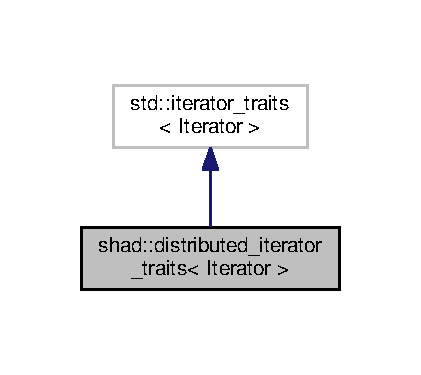
\includegraphics[width=202pt]{structshad_1_1distributed__iterator__traits__inherit__graph}
\end{center}
\end{figure}


Collaboration diagram for shad\-:\-:distributed\-\_\-iterator\-\_\-traits$<$ Iterator $>$\-:
\nopagebreak
\begin{figure}[H]
\begin{center}
\leavevmode
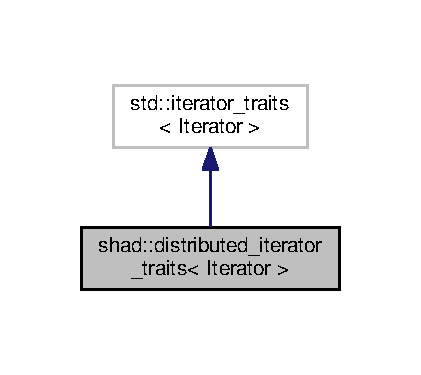
\includegraphics[width=202pt]{structshad_1_1distributed__iterator__traits__coll__graph}
\end{center}
\end{figure}
\subsection*{Public Types}
\begin{DoxyCompactItemize}
\item 
using \hyperlink{structshad_1_1distributed__iterator__traits_ad4f676acbe7b835cfda9f2ba84de0617}{difference\-\_\-type} = typename std\-::iterator\-\_\-traits$<$ Iterator $>$\-::\hyperlink{structshad_1_1distributed__iterator__traits_ad4f676acbe7b835cfda9f2ba84de0617}{difference\-\_\-type}
\item 
using \hyperlink{structshad_1_1distributed__iterator__traits_a67d1c97f6cfbb30068ed30d5fd5ef2bc}{value\-\_\-type} = typename std\-::iterator\-\_\-traits$<$ Iterator $>$\-::\hyperlink{structshad_1_1distributed__iterator__traits_a67d1c97f6cfbb30068ed30d5fd5ef2bc}{value\-\_\-type}
\item 
using \hyperlink{structshad_1_1distributed__iterator__traits_a3a4ebe1206d3e4d866752f2a3080f699}{pointer} = typename std\-::iterator\-\_\-traits$<$ Iterator $>$\-::\hyperlink{structshad_1_1distributed__iterator__traits_a3a4ebe1206d3e4d866752f2a3080f699}{pointer}
\item 
using \hyperlink{structshad_1_1distributed__iterator__traits_a82276f0370374d079f192c503f21b7a5}{reference} = typename std\-::iterator\-\_\-traits$<$ Iterator $>$\-::\hyperlink{structshad_1_1distributed__iterator__traits_a82276f0370374d079f192c503f21b7a5}{reference}
\item 
using \hyperlink{structshad_1_1distributed__iterator__traits_ae2c93d2849540657dd1f56c643d75c26}{iterator\-\_\-category} = typename std\-::iterator\-\_\-traits$<$ Iterator $>$\-::\hyperlink{structshad_1_1distributed__iterator__traits_ae2c93d2849540657dd1f56c643d75c26}{iterator\-\_\-category}
\item 
using \hyperlink{structshad_1_1distributed__iterator__traits_a7d2783595fdcaa86693980e101ce3c45}{local\-\_\-iterator\-\_\-range} = typename Iterator\-::local\-\_\-iterator\-\_\-range
\item 
using \hyperlink{structshad_1_1distributed__iterator__traits_afc228b2fcc17374bae1db42f3f666ac8}{local\-\_\-iterator\-\_\-type} = typename Iterator\-::local\-\_\-iterator\-\_\-type
\end{DoxyCompactItemize}
\subsection*{Static Public Member Functions}
\begin{DoxyCompactItemize}
\item 
static \hyperlink{classshad_1_1rt_1_1localities__range}{rt\-::localities\-\_\-range} \hyperlink{structshad_1_1distributed__iterator__traits_a479232b93342d09f2622f63c69f6f08a}{localities} (Iterator begin, Iterator end)
\item 
static \hyperlink{structshad_1_1distributed__iterator__traits_a7d2783595fdcaa86693980e101ce3c45}{local\-\_\-iterator\-\_\-range} \hyperlink{structshad_1_1distributed__iterator__traits_a29c17a7556893708bd90da103c1ee418}{local\-\_\-range} (Iterator begin, Iterator end)
\item 
static Iterator \hyperlink{structshad_1_1distributed__iterator__traits_a605bd0bf614f215ca3e13dd3052037e1}{iterator\-\_\-from\-\_\-local} (Iterator begin, Iterator end, \hyperlink{structshad_1_1distributed__iterator__traits_afc228b2fcc17374bae1db42f3f666ac8}{local\-\_\-iterator\-\_\-type} itr)
\end{DoxyCompactItemize}


\subsection{Member Typedef Documentation}
\hypertarget{structshad_1_1distributed__iterator__traits_ad4f676acbe7b835cfda9f2ba84de0617}{\index{shad\-::distributed\-\_\-iterator\-\_\-traits@{shad\-::distributed\-\_\-iterator\-\_\-traits}!difference\-\_\-type@{difference\-\_\-type}}
\index{difference\-\_\-type@{difference\-\_\-type}!shad::distributed_iterator_traits@{shad\-::distributed\-\_\-iterator\-\_\-traits}}
\subsubsection[{difference\-\_\-type}]{\setlength{\rightskip}{0pt plus 5cm}template$<$typename Iterator$>$ using {\bf shad\-::distributed\-\_\-iterator\-\_\-traits}$<$ Iterator $>$\-::{\bf difference\-\_\-type} =  typename std\-::iterator\-\_\-traits$<$Iterator$>$\-::{\bf difference\-\_\-type}}}\label{structshad_1_1distributed__iterator__traits_ad4f676acbe7b835cfda9f2ba84de0617}
\hypertarget{structshad_1_1distributed__iterator__traits_ae2c93d2849540657dd1f56c643d75c26}{\index{shad\-::distributed\-\_\-iterator\-\_\-traits@{shad\-::distributed\-\_\-iterator\-\_\-traits}!iterator\-\_\-category@{iterator\-\_\-category}}
\index{iterator\-\_\-category@{iterator\-\_\-category}!shad::distributed_iterator_traits@{shad\-::distributed\-\_\-iterator\-\_\-traits}}
\subsubsection[{iterator\-\_\-category}]{\setlength{\rightskip}{0pt plus 5cm}template$<$typename Iterator$>$ using {\bf shad\-::distributed\-\_\-iterator\-\_\-traits}$<$ Iterator $>$\-::{\bf iterator\-\_\-category} =  typename std\-::iterator\-\_\-traits$<$Iterator$>$\-::{\bf iterator\-\_\-category}}}\label{structshad_1_1distributed__iterator__traits_ae2c93d2849540657dd1f56c643d75c26}
\hypertarget{structshad_1_1distributed__iterator__traits_a7d2783595fdcaa86693980e101ce3c45}{\index{shad\-::distributed\-\_\-iterator\-\_\-traits@{shad\-::distributed\-\_\-iterator\-\_\-traits}!local\-\_\-iterator\-\_\-range@{local\-\_\-iterator\-\_\-range}}
\index{local\-\_\-iterator\-\_\-range@{local\-\_\-iterator\-\_\-range}!shad::distributed_iterator_traits@{shad\-::distributed\-\_\-iterator\-\_\-traits}}
\subsubsection[{local\-\_\-iterator\-\_\-range}]{\setlength{\rightskip}{0pt plus 5cm}template$<$typename Iterator$>$ using {\bf shad\-::distributed\-\_\-iterator\-\_\-traits}$<$ Iterator $>$\-::{\bf local\-\_\-iterator\-\_\-range} =  typename Iterator\-::local\-\_\-iterator\-\_\-range}}\label{structshad_1_1distributed__iterator__traits_a7d2783595fdcaa86693980e101ce3c45}
\hypertarget{structshad_1_1distributed__iterator__traits_afc228b2fcc17374bae1db42f3f666ac8}{\index{shad\-::distributed\-\_\-iterator\-\_\-traits@{shad\-::distributed\-\_\-iterator\-\_\-traits}!local\-\_\-iterator\-\_\-type@{local\-\_\-iterator\-\_\-type}}
\index{local\-\_\-iterator\-\_\-type@{local\-\_\-iterator\-\_\-type}!shad::distributed_iterator_traits@{shad\-::distributed\-\_\-iterator\-\_\-traits}}
\subsubsection[{local\-\_\-iterator\-\_\-type}]{\setlength{\rightskip}{0pt plus 5cm}template$<$typename Iterator$>$ using {\bf shad\-::distributed\-\_\-iterator\-\_\-traits}$<$ Iterator $>$\-::{\bf local\-\_\-iterator\-\_\-type} =  typename Iterator\-::local\-\_\-iterator\-\_\-type}}\label{structshad_1_1distributed__iterator__traits_afc228b2fcc17374bae1db42f3f666ac8}
\hypertarget{structshad_1_1distributed__iterator__traits_a3a4ebe1206d3e4d866752f2a3080f699}{\index{shad\-::distributed\-\_\-iterator\-\_\-traits@{shad\-::distributed\-\_\-iterator\-\_\-traits}!pointer@{pointer}}
\index{pointer@{pointer}!shad::distributed_iterator_traits@{shad\-::distributed\-\_\-iterator\-\_\-traits}}
\subsubsection[{pointer}]{\setlength{\rightskip}{0pt plus 5cm}template$<$typename Iterator$>$ using {\bf shad\-::distributed\-\_\-iterator\-\_\-traits}$<$ Iterator $>$\-::{\bf pointer} =  typename std\-::iterator\-\_\-traits$<$Iterator$>$\-::{\bf pointer}}}\label{structshad_1_1distributed__iterator__traits_a3a4ebe1206d3e4d866752f2a3080f699}
\hypertarget{structshad_1_1distributed__iterator__traits_a82276f0370374d079f192c503f21b7a5}{\index{shad\-::distributed\-\_\-iterator\-\_\-traits@{shad\-::distributed\-\_\-iterator\-\_\-traits}!reference@{reference}}
\index{reference@{reference}!shad::distributed_iterator_traits@{shad\-::distributed\-\_\-iterator\-\_\-traits}}
\subsubsection[{reference}]{\setlength{\rightskip}{0pt plus 5cm}template$<$typename Iterator$>$ using {\bf shad\-::distributed\-\_\-iterator\-\_\-traits}$<$ Iterator $>$\-::{\bf reference} =  typename std\-::iterator\-\_\-traits$<$Iterator$>$\-::{\bf reference}}}\label{structshad_1_1distributed__iterator__traits_a82276f0370374d079f192c503f21b7a5}
\hypertarget{structshad_1_1distributed__iterator__traits_a67d1c97f6cfbb30068ed30d5fd5ef2bc}{\index{shad\-::distributed\-\_\-iterator\-\_\-traits@{shad\-::distributed\-\_\-iterator\-\_\-traits}!value\-\_\-type@{value\-\_\-type}}
\index{value\-\_\-type@{value\-\_\-type}!shad::distributed_iterator_traits@{shad\-::distributed\-\_\-iterator\-\_\-traits}}
\subsubsection[{value\-\_\-type}]{\setlength{\rightskip}{0pt plus 5cm}template$<$typename Iterator$>$ using {\bf shad\-::distributed\-\_\-iterator\-\_\-traits}$<$ Iterator $>$\-::{\bf value\-\_\-type} =  typename std\-::iterator\-\_\-traits$<$Iterator$>$\-::{\bf value\-\_\-type}}}\label{structshad_1_1distributed__iterator__traits_a67d1c97f6cfbb30068ed30d5fd5ef2bc}


\subsection{Member Function Documentation}
\hypertarget{structshad_1_1distributed__iterator__traits_a605bd0bf614f215ca3e13dd3052037e1}{\index{shad\-::distributed\-\_\-iterator\-\_\-traits@{shad\-::distributed\-\_\-iterator\-\_\-traits}!iterator\-\_\-from\-\_\-local@{iterator\-\_\-from\-\_\-local}}
\index{iterator\-\_\-from\-\_\-local@{iterator\-\_\-from\-\_\-local}!shad::distributed_iterator_traits@{shad\-::distributed\-\_\-iterator\-\_\-traits}}
\subsubsection[{iterator\-\_\-from\-\_\-local}]{\setlength{\rightskip}{0pt plus 5cm}template$<$typename Iterator$>$ static Iterator {\bf shad\-::distributed\-\_\-iterator\-\_\-traits}$<$ Iterator $>$\-::iterator\-\_\-from\-\_\-local (
\begin{DoxyParamCaption}
\item[{Iterator}]{begin, }
\item[{Iterator}]{end, }
\item[{{\bf local\-\_\-iterator\-\_\-type}}]{itr}
\end{DoxyParamCaption}
)\hspace{0.3cm}{\ttfamily [inline]}, {\ttfamily [static]}}}\label{structshad_1_1distributed__iterator__traits_a605bd0bf614f215ca3e13dd3052037e1}
\hypertarget{structshad_1_1distributed__iterator__traits_a29c17a7556893708bd90da103c1ee418}{\index{shad\-::distributed\-\_\-iterator\-\_\-traits@{shad\-::distributed\-\_\-iterator\-\_\-traits}!local\-\_\-range@{local\-\_\-range}}
\index{local\-\_\-range@{local\-\_\-range}!shad::distributed_iterator_traits@{shad\-::distributed\-\_\-iterator\-\_\-traits}}
\subsubsection[{local\-\_\-range}]{\setlength{\rightskip}{0pt plus 5cm}template$<$typename Iterator$>$ static {\bf local\-\_\-iterator\-\_\-range} {\bf shad\-::distributed\-\_\-iterator\-\_\-traits}$<$ Iterator $>$\-::local\-\_\-range (
\begin{DoxyParamCaption}
\item[{Iterator}]{begin, }
\item[{Iterator}]{end}
\end{DoxyParamCaption}
)\hspace{0.3cm}{\ttfamily [inline]}, {\ttfamily [static]}}}\label{structshad_1_1distributed__iterator__traits_a29c17a7556893708bd90da103c1ee418}
\hypertarget{structshad_1_1distributed__iterator__traits_a479232b93342d09f2622f63c69f6f08a}{\index{shad\-::distributed\-\_\-iterator\-\_\-traits@{shad\-::distributed\-\_\-iterator\-\_\-traits}!localities@{localities}}
\index{localities@{localities}!shad::distributed_iterator_traits@{shad\-::distributed\-\_\-iterator\-\_\-traits}}
\subsubsection[{localities}]{\setlength{\rightskip}{0pt plus 5cm}template$<$typename Iterator$>$ static {\bf rt\-::localities\-\_\-range} {\bf shad\-::distributed\-\_\-iterator\-\_\-traits}$<$ Iterator $>$\-::localities (
\begin{DoxyParamCaption}
\item[{Iterator}]{begin, }
\item[{Iterator}]{end}
\end{DoxyParamCaption}
)\hspace{0.3cm}{\ttfamily [inline]}, {\ttfamily [static]}}}\label{structshad_1_1distributed__iterator__traits_a479232b93342d09f2622f63c69f6f08a}


The documentation for this struct was generated from the following file\-:\begin{DoxyCompactItemize}
\item 
include/shad/\hyperlink{distributed__iterator__traits_8h}{distributed\-\_\-iterator\-\_\-traits.\-h}\end{DoxyCompactItemize}

\hypertarget{structshad_1_1distributed__parallel__tag}{\section{shad\-:\-:distributed\-\_\-parallel\-\_\-tag Struct Reference}
\label{structshad_1_1distributed__parallel__tag}\index{shad\-::distributed\-\_\-parallel\-\_\-tag@{shad\-::distributed\-\_\-parallel\-\_\-tag}}
}


{\ttfamily \#include $<$shad/core/execution.\-h$>$}



The documentation for this struct was generated from the following file\-:\begin{DoxyCompactItemize}
\item 
include/shad/core/\hyperlink{execution_8h}{execution.\-h}\end{DoxyCompactItemize}

\hypertarget{structshad_1_1distributed__random__access__iterator__trait}{\section{shad\-:\-:distributed\-\_\-random\-\_\-access\-\_\-iterator\-\_\-trait$<$ Iterator $>$ Struct Template Reference}
\label{structshad_1_1distributed__random__access__iterator__trait}\index{shad\-::distributed\-\_\-random\-\_\-access\-\_\-iterator\-\_\-trait$<$ Iterator $>$@{shad\-::distributed\-\_\-random\-\_\-access\-\_\-iterator\-\_\-trait$<$ Iterator $>$}}
}


{\ttfamily \#include $<$shad/distributed\-\_\-iterator\-\_\-traits.\-h$>$}



Inheritance diagram for shad\-:\-:distributed\-\_\-random\-\_\-access\-\_\-iterator\-\_\-trait$<$ Iterator $>$\-:
\nopagebreak
\begin{figure}[H]
\begin{center}
\leavevmode
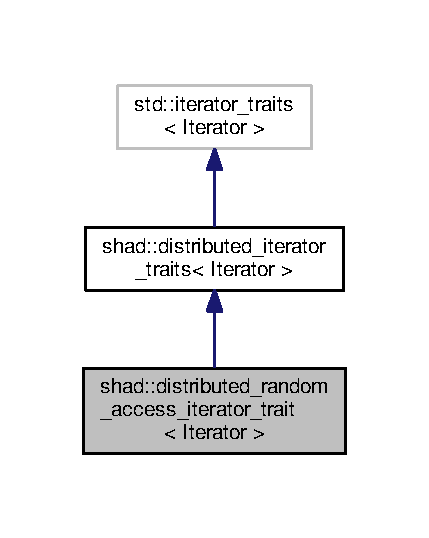
\includegraphics[width=206pt]{structshad_1_1distributed__random__access__iterator__trait__inherit__graph}
\end{center}
\end{figure}


Collaboration diagram for shad\-:\-:distributed\-\_\-random\-\_\-access\-\_\-iterator\-\_\-trait$<$ Iterator $>$\-:
\nopagebreak
\begin{figure}[H]
\begin{center}
\leavevmode
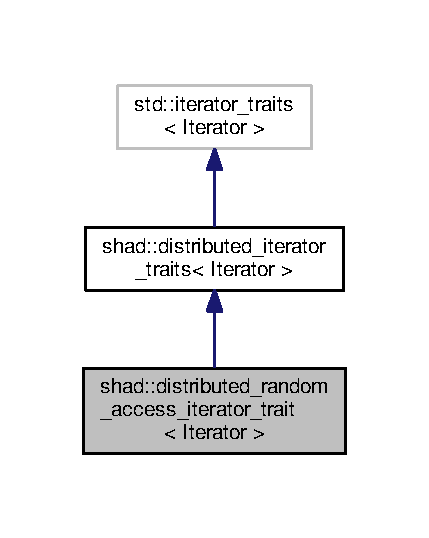
\includegraphics[width=206pt]{structshad_1_1distributed__random__access__iterator__trait__coll__graph}
\end{center}
\end{figure}
\subsection*{Public Types}
\begin{DoxyCompactItemize}
\item 
using \hyperlink{structshad_1_1distributed__random__access__iterator__trait_a8b61d58bf5959893ece6c9f38a1acf5d}{value\-\_\-type} = typename \hyperlink{structshad_1_1distributed__iterator__traits}{distributed\-\_\-iterator\-\_\-traits}$<$ Iterator $>$\-::\hyperlink{structshad_1_1distributed__iterator__traits_a67d1c97f6cfbb30068ed30d5fd5ef2bc}{value\-\_\-type}
\item 
using \hyperlink{structshad_1_1distributed__random__access__iterator__trait_aa7a80d89b4f5361c95d2cf7c682dc890}{pointer} = typename \hyperlink{structshad_1_1distributed__iterator__traits}{distributed\-\_\-iterator\-\_\-traits}$<$ Iterator $>$\-::\hyperlink{structshad_1_1distributed__iterator__traits_a3a4ebe1206d3e4d866752f2a3080f699}{pointer}
\item 
using \hyperlink{structshad_1_1distributed__random__access__iterator__trait_a67a58fe073cae4c0f77eb9ea96844bc1}{reference} = typename \hyperlink{structshad_1_1distributed__iterator__traits}{distributed\-\_\-iterator\-\_\-traits}$<$ Iterator $>$\-::\hyperlink{structshad_1_1distributed__iterator__traits_a82276f0370374d079f192c503f21b7a5}{reference}
\item 
using \hyperlink{structshad_1_1distributed__random__access__iterator__trait_a6794da2277108e23065517078bbf8e93}{iterator\-\_\-category} = typename \hyperlink{structshad_1_1distributed__iterator__traits}{distributed\-\_\-iterator\-\_\-traits}$<$ Iterator $>$\-::\hyperlink{structshad_1_1distributed__iterator__traits_ae2c93d2849540657dd1f56c643d75c26}{iterator\-\_\-category}
\item 
using \hyperlink{structshad_1_1distributed__random__access__iterator__trait_a8981d6d76b421929c62efdd94ea806a3}{distribution\-\_\-range} = typename Iterator\-::distribution\-\_\-range
\end{DoxyCompactItemize}
\subsection*{Static Public Member Functions}
\begin{DoxyCompactItemize}
\item 
static \hyperlink{structshad_1_1distributed__random__access__iterator__trait_a8981d6d76b421929c62efdd94ea806a3}{distribution\-\_\-range} \hyperlink{structshad_1_1distributed__random__access__iterator__trait_ac99f0d323413ef3ac676168b00e43cb9}{distribution} (Iterator begin, Iterator end)
\end{DoxyCompactItemize}


\subsection{Member Typedef Documentation}
\hypertarget{structshad_1_1distributed__random__access__iterator__trait_a8981d6d76b421929c62efdd94ea806a3}{\index{shad\-::distributed\-\_\-random\-\_\-access\-\_\-iterator\-\_\-trait@{shad\-::distributed\-\_\-random\-\_\-access\-\_\-iterator\-\_\-trait}!distribution\-\_\-range@{distribution\-\_\-range}}
\index{distribution\-\_\-range@{distribution\-\_\-range}!shad::distributed_random_access_iterator_trait@{shad\-::distributed\-\_\-random\-\_\-access\-\_\-iterator\-\_\-trait}}
\subsubsection[{distribution\-\_\-range}]{\setlength{\rightskip}{0pt plus 5cm}template$<$typename Iterator $>$ using {\bf shad\-::distributed\-\_\-random\-\_\-access\-\_\-iterator\-\_\-trait}$<$ Iterator $>$\-::{\bf distribution\-\_\-range} =  typename Iterator\-::distribution\-\_\-range}}\label{structshad_1_1distributed__random__access__iterator__trait_a8981d6d76b421929c62efdd94ea806a3}
\hypertarget{structshad_1_1distributed__random__access__iterator__trait_a6794da2277108e23065517078bbf8e93}{\index{shad\-::distributed\-\_\-random\-\_\-access\-\_\-iterator\-\_\-trait@{shad\-::distributed\-\_\-random\-\_\-access\-\_\-iterator\-\_\-trait}!iterator\-\_\-category@{iterator\-\_\-category}}
\index{iterator\-\_\-category@{iterator\-\_\-category}!shad::distributed_random_access_iterator_trait@{shad\-::distributed\-\_\-random\-\_\-access\-\_\-iterator\-\_\-trait}}
\subsubsection[{iterator\-\_\-category}]{\setlength{\rightskip}{0pt plus 5cm}template$<$typename Iterator $>$ using {\bf shad\-::distributed\-\_\-random\-\_\-access\-\_\-iterator\-\_\-trait}$<$ Iterator $>$\-::{\bf iterator\-\_\-category} =  typename {\bf distributed\-\_\-iterator\-\_\-traits}$<$Iterator$>$\-::{\bf iterator\-\_\-category}}}\label{structshad_1_1distributed__random__access__iterator__trait_a6794da2277108e23065517078bbf8e93}
\hypertarget{structshad_1_1distributed__random__access__iterator__trait_aa7a80d89b4f5361c95d2cf7c682dc890}{\index{shad\-::distributed\-\_\-random\-\_\-access\-\_\-iterator\-\_\-trait@{shad\-::distributed\-\_\-random\-\_\-access\-\_\-iterator\-\_\-trait}!pointer@{pointer}}
\index{pointer@{pointer}!shad::distributed_random_access_iterator_trait@{shad\-::distributed\-\_\-random\-\_\-access\-\_\-iterator\-\_\-trait}}
\subsubsection[{pointer}]{\setlength{\rightskip}{0pt plus 5cm}template$<$typename Iterator $>$ using {\bf shad\-::distributed\-\_\-random\-\_\-access\-\_\-iterator\-\_\-trait}$<$ Iterator $>$\-::{\bf pointer} =  typename {\bf distributed\-\_\-iterator\-\_\-traits}$<$Iterator$>$\-::{\bf pointer}}}\label{structshad_1_1distributed__random__access__iterator__trait_aa7a80d89b4f5361c95d2cf7c682dc890}
\hypertarget{structshad_1_1distributed__random__access__iterator__trait_a67a58fe073cae4c0f77eb9ea96844bc1}{\index{shad\-::distributed\-\_\-random\-\_\-access\-\_\-iterator\-\_\-trait@{shad\-::distributed\-\_\-random\-\_\-access\-\_\-iterator\-\_\-trait}!reference@{reference}}
\index{reference@{reference}!shad::distributed_random_access_iterator_trait@{shad\-::distributed\-\_\-random\-\_\-access\-\_\-iterator\-\_\-trait}}
\subsubsection[{reference}]{\setlength{\rightskip}{0pt plus 5cm}template$<$typename Iterator $>$ using {\bf shad\-::distributed\-\_\-random\-\_\-access\-\_\-iterator\-\_\-trait}$<$ Iterator $>$\-::{\bf reference} =  typename {\bf distributed\-\_\-iterator\-\_\-traits}$<$Iterator$>$\-::{\bf reference}}}\label{structshad_1_1distributed__random__access__iterator__trait_a67a58fe073cae4c0f77eb9ea96844bc1}
\hypertarget{structshad_1_1distributed__random__access__iterator__trait_a8b61d58bf5959893ece6c9f38a1acf5d}{\index{shad\-::distributed\-\_\-random\-\_\-access\-\_\-iterator\-\_\-trait@{shad\-::distributed\-\_\-random\-\_\-access\-\_\-iterator\-\_\-trait}!value\-\_\-type@{value\-\_\-type}}
\index{value\-\_\-type@{value\-\_\-type}!shad::distributed_random_access_iterator_trait@{shad\-::distributed\-\_\-random\-\_\-access\-\_\-iterator\-\_\-trait}}
\subsubsection[{value\-\_\-type}]{\setlength{\rightskip}{0pt plus 5cm}template$<$typename Iterator $>$ using {\bf shad\-::distributed\-\_\-random\-\_\-access\-\_\-iterator\-\_\-trait}$<$ Iterator $>$\-::{\bf value\-\_\-type} =  typename {\bf distributed\-\_\-iterator\-\_\-traits}$<$Iterator$>$\-::{\bf value\-\_\-type}}}\label{structshad_1_1distributed__random__access__iterator__trait_a8b61d58bf5959893ece6c9f38a1acf5d}


\subsection{Member Function Documentation}
\hypertarget{structshad_1_1distributed__random__access__iterator__trait_ac99f0d323413ef3ac676168b00e43cb9}{\index{shad\-::distributed\-\_\-random\-\_\-access\-\_\-iterator\-\_\-trait@{shad\-::distributed\-\_\-random\-\_\-access\-\_\-iterator\-\_\-trait}!distribution@{distribution}}
\index{distribution@{distribution}!shad::distributed_random_access_iterator_trait@{shad\-::distributed\-\_\-random\-\_\-access\-\_\-iterator\-\_\-trait}}
\subsubsection[{distribution}]{\setlength{\rightskip}{0pt plus 5cm}template$<$typename Iterator $>$ static {\bf distribution\-\_\-range} {\bf shad\-::distributed\-\_\-random\-\_\-access\-\_\-iterator\-\_\-trait}$<$ Iterator $>$\-::distribution (
\begin{DoxyParamCaption}
\item[{Iterator}]{begin, }
\item[{Iterator}]{end}
\end{DoxyParamCaption}
)\hspace{0.3cm}{\ttfamily [inline]}, {\ttfamily [static]}}}\label{structshad_1_1distributed__random__access__iterator__trait_ac99f0d323413ef3ac676168b00e43cb9}


The documentation for this struct was generated from the following file\-:\begin{DoxyCompactItemize}
\item 
include/shad/\hyperlink{distributed__iterator__traits_8h}{distributed\-\_\-iterator\-\_\-traits.\-h}\end{DoxyCompactItemize}

\hypertarget{structshad_1_1distributed__sequential__tag}{\section{shad\-:\-:distributed\-\_\-sequential\-\_\-tag Struct Reference}
\label{structshad_1_1distributed__sequential__tag}\index{shad\-::distributed\-\_\-sequential\-\_\-tag@{shad\-::distributed\-\_\-sequential\-\_\-tag}}
}


{\ttfamily \#include $<$shad/core/execution.\-h$>$}



The documentation for this struct was generated from the following file\-:\begin{DoxyCompactItemize}
\item 
include/shad/core/\hyperlink{execution_8h}{execution.\-h}\end{DoxyCompactItemize}

\hypertarget{classshad_1_1EdgeIndex}{\section{shad\-:\-:Edge\-Index$<$ Src\-T, Dest\-T, Storage\-T $>$ Class Template Reference}
\label{classshad_1_1EdgeIndex}\index{shad\-::\-Edge\-Index$<$ Src\-T, Dest\-T, Storage\-T $>$@{shad\-::\-Edge\-Index$<$ Src\-T, Dest\-T, Storage\-T $>$}}
}


The \hyperlink{classshad_1_1EdgeIndex}{Edge\-Index} data structure.  




{\ttfamily \#include $<$shad/extensions/graph\-\_\-library/edge\-\_\-index.\-h$>$}



Inheritance diagram for shad\-:\-:Edge\-Index$<$ Src\-T, Dest\-T, Storage\-T $>$\-:
\nopagebreak
\begin{figure}[H]
\begin{center}
\leavevmode
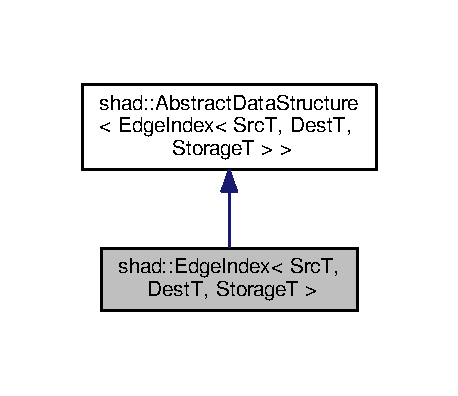
\includegraphics[width=220pt]{classshad_1_1EdgeIndex__inherit__graph}
\end{center}
\end{figure}


Collaboration diagram for shad\-:\-:Edge\-Index$<$ Src\-T, Dest\-T, Storage\-T $>$\-:
\nopagebreak
\begin{figure}[H]
\begin{center}
\leavevmode
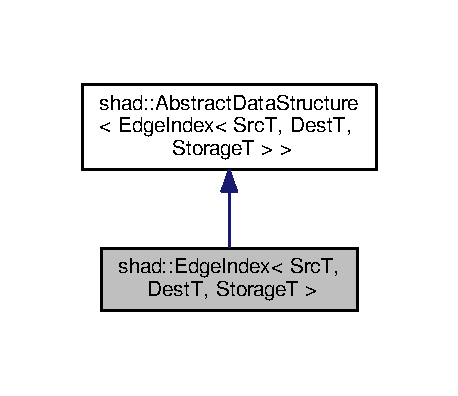
\includegraphics[width=220pt]{classshad_1_1EdgeIndex__coll__graph}
\end{center}
\end{figure}
\subsection*{Classes}
\begin{DoxyCompactItemize}
\item 
struct \hyperlink{structshad_1_1EdgeIndex_1_1EntryT}{Entry\-T}
\end{DoxyCompactItemize}
\subsection*{Public Types}
\begin{DoxyCompactItemize}
\item 
using \hyperlink{classshad_1_1EdgeIndex_ac1849d1d8dc7f32e2ca56fa224308ef2}{Object\-I\-D} = typename \hyperlink{classshad_1_1AbstractDataStructure}{Abstract\-Data\-Structure}$<$ \hyperlink{classshad_1_1EdgeIndex}{Edge\-Index}$<$ Src\-T, Dest\-T, Storage\-T $>$$>$\-::\hyperlink{classshad_1_1EdgeIndex_ac1849d1d8dc7f32e2ca56fa224308ef2}{Object\-I\-D}
\item 
using \hyperlink{classshad_1_1EdgeIndex_ae6b70863258ef3efebc3868e5c791a0d}{Edge\-List\-Ptr} = typename \hyperlink{classshad_1_1AbstractDataStructure}{Abstract\-Data\-Structure}$<$ \hyperlink{classshad_1_1EdgeIndex}{Edge\-Index}$<$ Src\-T, Dest\-T, Storage\-T $>$$>$\-::\hyperlink{classshad_1_1AbstractDataStructure_a8bb29450966955c546d40421ce46316f}{Shared\-Ptr}
\item 
using \hyperlink{classshad_1_1EdgeIndex_a10fd1a7498be01373f022c3e4445bd92}{Src\-Type} = Src\-T
\item 
using \hyperlink{classshad_1_1EdgeIndex_a1fe85e04eb8fbc43233e1656e93ca4fd}{Dest\-Type} = Dest\-T
\item 
using \hyperlink{classshad_1_1EdgeIndex_af0fe2f8cb6950ca82e97085c0baedf90}{L\-Idx\-T} = \hyperlink{classshad_1_1LocalEdgeIndex}{Local\-Edge\-Index}$<$ Src\-T, Dest\-T, Storage\-T $>$
\item 
using \hyperlink{classshad_1_1EdgeIndex_a8beb31c05450d63d7add3f9408c9943a}{Idx\-T} = \hyperlink{classshad_1_1EdgeIndex}{Edge\-Index}$<$ Src\-T, Dest\-T, Storage\-T $>$
\item 
using \hyperlink{classshad_1_1EdgeIndex_af749b171d243a86058fffe96247d42f5}{Buffers\-Vector} = typename impl\-::\-Buffers\-Vector$<$ \hyperlink{structshad_1_1EdgeIndex_1_1EntryT}{Entry\-T}, \hyperlink{classshad_1_1EdgeIndex}{Edge\-Index}$<$ Src\-T, Dest\-T, Storage\-T $>$$>$
\end{DoxyCompactItemize}
\subsection*{Public Member Functions}
\begin{DoxyCompactItemize}
\item 
\hyperlink{classshad_1_1EdgeIndex_ac1849d1d8dc7f32e2ca56fa224308ef2}{Object\-I\-D} \hyperlink{classshad_1_1EdgeIndex_aa07ea25da27d521c32434d0dc3dc5ac9}{Get\-Global\-I\-D} () const 
\begin{DoxyCompactList}\small\item\em Getter of the Global Identifier. \end{DoxyCompactList}\item 
size\-\_\-t \hyperlink{classshad_1_1EdgeIndex_a2e4c3f4a29d28742879d3119d835fc57}{Size} () const 
\begin{DoxyCompactList}\small\item\em Overall size of the edge index (number of unique sources). \end{DoxyCompactList}\item 
size\-\_\-t \hyperlink{classshad_1_1EdgeIndex_ac2177910ddf94f52f4b1833a72509992}{Num\-Edges} ()
\begin{DoxyCompactList}\small\item\em Overall number of edges in the index. \end{DoxyCompactList}\item 
void \hyperlink{classshad_1_1EdgeIndex_a410c822912b1335afaa8c393ebeb5c2c}{Insert} (const Src\-T \&src, const Dest\-T \&dest)
\begin{DoxyCompactList}\small\item\em Insert an edge in the index. \end{DoxyCompactList}\item 
void \hyperlink{classshad_1_1EdgeIndex_a28391328c8882398f6452f7987ecbe53}{Async\-Insert} (\hyperlink{classshad_1_1rt_1_1Handle}{rt\-::\-Handle} \&handle, const Src\-T \&src, const Dest\-T \&dest)
\begin{DoxyCompactList}\small\item\em Asynchronously insert an edge in the index. \end{DoxyCompactList}\item 
void \hyperlink{classshad_1_1EdgeIndex_a3d46667ec205db01b0fd6e9d418cf192}{Insert\-Edge\-List} (const Src\-T \&src, Dest\-T $\ast$destinations, size\-\_\-t num\-Dest, bool overwrite=true)
\begin{DoxyCompactList}\small\item\em Insert an edge list in the index. \end{DoxyCompactList}\item 
void \hyperlink{classshad_1_1EdgeIndex_ad27778c664727b3784988250c5623ab6}{Async\-Insert\-Edge\-List} (\hyperlink{classshad_1_1rt_1_1Handle}{rt\-::\-Handle} \&handle, const Src\-T \&src, Dest\-T $\ast$destinations, size\-\_\-t num\-Dest, bool overwrite=true)
\begin{DoxyCompactList}\small\item\em Asynchronously insert an edge list in the index. \end{DoxyCompactList}\item 
void \hyperlink{classshad_1_1EdgeIndex_a9d9a45b30b9a274674e8180d6468f6cc}{Async\-Get\-Neighbors} (\hyperlink{classshad_1_1rt_1_1Handle}{rt\-::\-Handle} \&handle, const Src\-T src, typename Storage\-T\-::\-Neighbor\-List\-Storage\-T $\ast$$\ast$res)
\begin{DoxyCompactList}\small\item\em Asynchronously retrieve the neighbors list of a given vertex. \end{DoxyCompactList}\item 
void \hyperlink{classshad_1_1EdgeIndex_a8b7bc20d65a535f0ec1b568d7cbbca4b}{Get\-Neighbors} (const Src\-T \&src, typename Storage\-T\-::\-Neighbor\-List\-Storage\-T $\ast$res)
\begin{DoxyCompactList}\small\item\em Retrieve the neighbors list of a given vertex. \end{DoxyCompactList}\item 
size\-\_\-t \hyperlink{classshad_1_1EdgeIndex_a39bf8088eb8689211e0273dc1d7e3b3a}{Get\-Degree} (const Src\-T \&src)
\begin{DoxyCompactList}\small\item\em Number of neighbors of a given vertex. \end{DoxyCompactList}\item 
void \hyperlink{classshad_1_1EdgeIndex_a1b2fbd03993f2687ca92b91e22667bb3}{Buffered\-Insert} (const Src\-T \&src, const Dest\-T \&dest)
\begin{DoxyCompactList}\small\item\em Buffered Insert method. \end{DoxyCompactList}\item 
void \hyperlink{classshad_1_1EdgeIndex_aaad1cccd3da96c4e957fad51f4b60f5d}{Buffered\-Async\-Insert} (\hyperlink{classshad_1_1rt_1_1Handle}{rt\-::\-Handle} \&handle, const Src\-T \&src, const Dest\-T \&dest)
\begin{DoxyCompactList}\small\item\em Asynchronous Buffered Insert method. \end{DoxyCompactList}\item 
void \hyperlink{classshad_1_1EdgeIndex_a4b02ebf2ea13561e06470dabeaa957ca}{Wait\-For\-Buffered\-Insert} ()
\begin{DoxyCompactList}\small\item\em Finalize method for buffered insertions. \end{DoxyCompactList}\item 
void \hyperlink{classshad_1_1EdgeIndex_ac763297b97967b220bb9658927b91bab}{Erase} (const Src\-T \&src, const Dest\-T \&dest)
\begin{DoxyCompactList}\small\item\em Delete an edge. \end{DoxyCompactList}\item 
void \hyperlink{classshad_1_1EdgeIndex_a474b38452f60fe74c6230e9e10be6a35}{Async\-Erase} (\hyperlink{classshad_1_1rt_1_1Handle}{rt\-::\-Handle} \&handle, const Src\-T \&src, const Dest\-T \&dest)
\begin{DoxyCompactList}\small\item\em Asynchronously delete an edge. \end{DoxyCompactList}\item 
void \hyperlink{classshad_1_1EdgeIndex_aa792333e7ef7cc1c1883fa7e6e8c6c3f}{Erase} (const Src\-T \&src)
\begin{DoxyCompactList}\small\item\em Remove a vertex from the edge index. \end{DoxyCompactList}\item 
void \hyperlink{classshad_1_1EdgeIndex_a79eb64ffbc08c73aa03d03efe5fdd312}{Clear} ()
\begin{DoxyCompactList}\small\item\em Clear the content of the edge index. \end{DoxyCompactList}\item 
void \hyperlink{classshad_1_1EdgeIndex_afab5d3fe70db0c4f96f2516e08c8fdee}{Buffer\-Entry\-Insert} (const \hyperlink{structshad_1_1EdgeIndex_1_1EntryT}{Entry\-T} \&entry)
\item 
{\footnotesize template$<$typename Apply\-Fun\-T , typename... Args$>$ }\\void \hyperlink{classshad_1_1EdgeIndex_a26dfd4d48e1f16ac4c988ec49dc2ffb4}{For\-Each\-Neighbor} (const Src\-T \&src, Apply\-Fun\-T \&\&function, Args \&...args)
\begin{DoxyCompactList}\small\item\em Apply a user-\/defined function to each neighbor of a given vertex. \end{DoxyCompactList}\item 
{\footnotesize template$<$typename Apply\-Fun\-T , typename... Args$>$ }\\void \hyperlink{classshad_1_1EdgeIndex_a4006c67fe1a61a5b83d8e3f9bebd616f}{Async\-For\-Each\-Neighbor} (\hyperlink{classshad_1_1rt_1_1Handle}{rt\-::\-Handle} \&handle, const Src\-T \&src, Apply\-Fun\-T \&\&function, Args \&...args)
\begin{DoxyCompactList}\small\item\em Asynchronously apply a user-\/defined function to each neighbor of a given vertex. \end{DoxyCompactList}\item 
{\footnotesize template$<$typename Apply\-Fun\-T , typename... Args$>$ }\\void \hyperlink{classshad_1_1EdgeIndex_a50ba7449742c1ee2a06ba4529493b656}{For\-Each\-Vertex} (Apply\-Fun\-T \&\&function, Args \&...args)
\begin{DoxyCompactList}\small\item\em Apply a user-\/defined function to each vertex. \end{DoxyCompactList}\item 
{\footnotesize template$<$typename Apply\-Fun\-T , typename... Args$>$ }\\void \hyperlink{classshad_1_1EdgeIndex_a7e7ad3189f35af48bdd627c086bbc00c}{Async\-For\-Each\-Vertex} (\hyperlink{classshad_1_1rt_1_1Handle}{rt\-::\-Handle} \&handle, Apply\-Fun\-T \&\&function, Args \&...args)
\begin{DoxyCompactList}\small\item\em Apply a user-\/defined function to each vertex. \end{DoxyCompactList}\item 
{\footnotesize template$<$typename Apply\-Fun\-T , typename... Args$>$ }\\void \hyperlink{classshad_1_1EdgeIndex_ad6ffc821277ec7cbb19d47cca6fd08f8}{For\-Each\-Edge} (Apply\-Fun\-T \&\&function, Args \&...args)
\begin{DoxyCompactList}\small\item\em Apply a user-\/defined function to each edge. \end{DoxyCompactList}\item 
{\footnotesize template$<$typename Apply\-Fun\-T , typename... Args$>$ }\\void \hyperlink{classshad_1_1EdgeIndex_a0388260052d7d512e99b344ec8630462}{Async\-For\-Each\-Edge} (\hyperlink{classshad_1_1rt_1_1Handle}{rt\-::\-Handle} \&handle, Apply\-Fun\-T \&\&function, Args \&...args)
\begin{DoxyCompactList}\small\item\em Asynchronously apply a user-\/defined function to each edge. \end{DoxyCompactList}\item 
\hyperlink{classshad_1_1LocalEdgeIndex}{Local\-Edge\-Index}$<$ Src\-T, Dest\-T, \\*
Storage\-T $>$ $\ast$ \hyperlink{classshad_1_1EdgeIndex_a3865d359b5915da27c1ed724e2586be1}{Get\-Local\-Index\-Ptr} ()
\item 
bool \hyperlink{classshad_1_1EdgeIndex_a081298237f8cec930e4f6104b371ab7b}{Get\-Vertex\-Attributes} (const Src\-T \&src, typename Storage\-T\-::\-Src\-Attributes\-T $\ast$attr)
\begin{DoxyCompactList}\small\item\em Retrieve the attributes of a given vertex. \end{DoxyCompactList}\item 
{\footnotesize template$<$typename Apply\-Fun\-T , typename... Args$>$ }\\void \hyperlink{classshad_1_1EdgeIndex_a41732ef7cd7c4824d752525110c58db8}{Vertex\-Attributes\-Apply} (const Src\-T \&src, Apply\-Fun\-T \&\&function, Args \&...args)
\begin{DoxyCompactList}\small\item\em Apply a user-\/defined function to the attributes of a given vertex. \end{DoxyCompactList}\end{DoxyCompactItemize}
\subsection*{Static Public Member Functions}
\begin{DoxyCompactItemize}
\item 
static Edge\-Index\-Ptr \hyperlink{classshad_1_1EdgeIndex_a3f3094d51e6275b382a72c552cca58a4}{Create} (const size\-\_\-t num\-Vertices)
\begin{DoxyCompactList}\small\item\em Create method. \end{DoxyCompactList}\end{DoxyCompactItemize}
\subsection*{Protected Member Functions}
\begin{DoxyCompactItemize}
\item 
\hyperlink{classshad_1_1EdgeIndex_a4d82e057adb441e486fd3500a2633f48}{Edge\-Index} (\hyperlink{classshad_1_1EdgeIndex_ac1849d1d8dc7f32e2ca56fa224308ef2}{Object\-I\-D} oid, const size\-\_\-t num\-Vertices)
\item 
\hyperlink{classshad_1_1EdgeIndex_af18ce9911aa0239fa4a3e02d66175c75}{Edge\-Index} (\hyperlink{classshad_1_1EdgeIndex_ac1849d1d8dc7f32e2ca56fa224308ef2}{Object\-I\-D} oid, const size\-\_\-t num\-Vertices, const typename Storage\-T\-::\-Src\-Attributes\-T \&init\-Attr)
\end{DoxyCompactItemize}
\subsection*{Friends}
\begin{DoxyCompactItemize}
\item 
{\footnotesize template$<$typename $>$ }\\class \hyperlink{classshad_1_1EdgeIndex_ab18afa4496cc863ddc11bab94b2adf57}{Abstract\-Data\-Structure}
\item 
{\footnotesize template$<$typename , typename , typename $>$ }\\class \hyperlink{classshad_1_1EdgeIndex_afc8d107f39c9ea0b8848ea970eb36b93}{Local\-Edge\-Index}
\end{DoxyCompactItemize}
\subsection*{Additional Inherited Members}


\subsection{Detailed Description}
\subsubsection*{template$<$typename Src\-T, typename Dest\-T, typename Storage\-T = Default\-Edge\-Index\-Storage$<$\-Src\-T, Dest\-T$>$$>$class shad\-::\-Edge\-Index$<$ Src\-T, Dest\-T, Storage\-T $>$}

The \hyperlink{classshad_1_1EdgeIndex}{Edge\-Index} data structure. 

S\-H\-A\-D's \hyperlink{classshad_1_1EdgeIndex}{Edge\-Index} is a thread-\/safe, associative container, representing a collection of neighbors lists of a graph. 
\begin{DoxyTemplParams}{Template Parameters}
{\em Src\-T} & type of source vertices (used as identifiers). \\
\hline
{\em Dest\-T} & type of destination vertices (used as identifiers). \\
\hline
\end{DoxyTemplParams}
\begin{DoxyWarning}{Warning}
obects of type Src\-T and Dest\-T need to be trivially copiable. 
\end{DoxyWarning}

\begin{DoxyTemplParams}{Template Parameters}
{\em Storage\-T} & \hyperlink{classshad_1_1EdgeIndex}{Edge\-Index} local storage. Default is a map of sets. \\
\hline
\end{DoxyTemplParams}


\subsection{Member Typedef Documentation}
\hypertarget{classshad_1_1EdgeIndex_af749b171d243a86058fffe96247d42f5}{\index{shad\-::\-Edge\-Index@{shad\-::\-Edge\-Index}!Buffers\-Vector@{Buffers\-Vector}}
\index{Buffers\-Vector@{Buffers\-Vector}!shad::EdgeIndex@{shad\-::\-Edge\-Index}}
\subsubsection[{Buffers\-Vector}]{\setlength{\rightskip}{0pt plus 5cm}template$<$typename Src\-T , typename Dest\-T , typename Storage\-T  = Default\-Edge\-Index\-Storage$<$\-Src\-T, Dest\-T$>$$>$ using {\bf shad\-::\-Edge\-Index}$<$ Src\-T, Dest\-T, Storage\-T $>$\-::{\bf Buffers\-Vector} =  typename impl\-::\-Buffers\-Vector$<${\bf Entry\-T}, {\bf Edge\-Index}$<$Src\-T, Dest\-T, Storage\-T$>$$>$}}\label{classshad_1_1EdgeIndex_af749b171d243a86058fffe96247d42f5}
\hypertarget{classshad_1_1EdgeIndex_a1fe85e04eb8fbc43233e1656e93ca4fd}{\index{shad\-::\-Edge\-Index@{shad\-::\-Edge\-Index}!Dest\-Type@{Dest\-Type}}
\index{Dest\-Type@{Dest\-Type}!shad::EdgeIndex@{shad\-::\-Edge\-Index}}
\subsubsection[{Dest\-Type}]{\setlength{\rightskip}{0pt plus 5cm}template$<$typename Src\-T , typename Dest\-T , typename Storage\-T  = Default\-Edge\-Index\-Storage$<$\-Src\-T, Dest\-T$>$$>$ using {\bf shad\-::\-Edge\-Index}$<$ Src\-T, Dest\-T, Storage\-T $>$\-::{\bf Dest\-Type} =  Dest\-T}}\label{classshad_1_1EdgeIndex_a1fe85e04eb8fbc43233e1656e93ca4fd}
\hypertarget{classshad_1_1EdgeIndex_ae6b70863258ef3efebc3868e5c791a0d}{\index{shad\-::\-Edge\-Index@{shad\-::\-Edge\-Index}!Edge\-List\-Ptr@{Edge\-List\-Ptr}}
\index{Edge\-List\-Ptr@{Edge\-List\-Ptr}!shad::EdgeIndex@{shad\-::\-Edge\-Index}}
\subsubsection[{Edge\-List\-Ptr}]{\setlength{\rightskip}{0pt plus 5cm}template$<$typename Src\-T , typename Dest\-T , typename Storage\-T  = Default\-Edge\-Index\-Storage$<$\-Src\-T, Dest\-T$>$$>$ using {\bf shad\-::\-Edge\-Index}$<$ Src\-T, Dest\-T, Storage\-T $>$\-::{\bf Edge\-List\-Ptr} =  typename {\bf Abstract\-Data\-Structure}$<$ {\bf Edge\-Index}$<$Src\-T, Dest\-T, Storage\-T$>$$>$\-::{\bf Shared\-Ptr}}}\label{classshad_1_1EdgeIndex_ae6b70863258ef3efebc3868e5c791a0d}
\hypertarget{classshad_1_1EdgeIndex_a8beb31c05450d63d7add3f9408c9943a}{\index{shad\-::\-Edge\-Index@{shad\-::\-Edge\-Index}!Idx\-T@{Idx\-T}}
\index{Idx\-T@{Idx\-T}!shad::EdgeIndex@{shad\-::\-Edge\-Index}}
\subsubsection[{Idx\-T}]{\setlength{\rightskip}{0pt plus 5cm}template$<$typename Src\-T , typename Dest\-T , typename Storage\-T  = Default\-Edge\-Index\-Storage$<$\-Src\-T, Dest\-T$>$$>$ using {\bf shad\-::\-Edge\-Index}$<$ Src\-T, Dest\-T, Storage\-T $>$\-::{\bf Idx\-T} =  {\bf Edge\-Index}$<$Src\-T, Dest\-T, Storage\-T$>$}}\label{classshad_1_1EdgeIndex_a8beb31c05450d63d7add3f9408c9943a}
\hypertarget{classshad_1_1EdgeIndex_af0fe2f8cb6950ca82e97085c0baedf90}{\index{shad\-::\-Edge\-Index@{shad\-::\-Edge\-Index}!L\-Idx\-T@{L\-Idx\-T}}
\index{L\-Idx\-T@{L\-Idx\-T}!shad::EdgeIndex@{shad\-::\-Edge\-Index}}
\subsubsection[{L\-Idx\-T}]{\setlength{\rightskip}{0pt plus 5cm}template$<$typename Src\-T , typename Dest\-T , typename Storage\-T  = Default\-Edge\-Index\-Storage$<$\-Src\-T, Dest\-T$>$$>$ using {\bf shad\-::\-Edge\-Index}$<$ Src\-T, Dest\-T, Storage\-T $>$\-::{\bf L\-Idx\-T} =  {\bf Local\-Edge\-Index}$<$Src\-T, Dest\-T, Storage\-T$>$}}\label{classshad_1_1EdgeIndex_af0fe2f8cb6950ca82e97085c0baedf90}
\hypertarget{classshad_1_1EdgeIndex_ac1849d1d8dc7f32e2ca56fa224308ef2}{\index{shad\-::\-Edge\-Index@{shad\-::\-Edge\-Index}!Object\-I\-D@{Object\-I\-D}}
\index{Object\-I\-D@{Object\-I\-D}!shad::EdgeIndex@{shad\-::\-Edge\-Index}}
\subsubsection[{Object\-I\-D}]{\setlength{\rightskip}{0pt plus 5cm}template$<$typename Src\-T , typename Dest\-T , typename Storage\-T  = Default\-Edge\-Index\-Storage$<$\-Src\-T, Dest\-T$>$$>$ using {\bf shad\-::\-Edge\-Index}$<$ Src\-T, Dest\-T, Storage\-T $>$\-::{\bf Object\-I\-D} =  typename {\bf Abstract\-Data\-Structure}$<$ {\bf Edge\-Index}$<$Src\-T, Dest\-T, Storage\-T$>$$>$\-::{\bf Object\-I\-D}}}\label{classshad_1_1EdgeIndex_ac1849d1d8dc7f32e2ca56fa224308ef2}
\hypertarget{classshad_1_1EdgeIndex_a10fd1a7498be01373f022c3e4445bd92}{\index{shad\-::\-Edge\-Index@{shad\-::\-Edge\-Index}!Src\-Type@{Src\-Type}}
\index{Src\-Type@{Src\-Type}!shad::EdgeIndex@{shad\-::\-Edge\-Index}}
\subsubsection[{Src\-Type}]{\setlength{\rightskip}{0pt plus 5cm}template$<$typename Src\-T , typename Dest\-T , typename Storage\-T  = Default\-Edge\-Index\-Storage$<$\-Src\-T, Dest\-T$>$$>$ using {\bf shad\-::\-Edge\-Index}$<$ Src\-T, Dest\-T, Storage\-T $>$\-::{\bf Src\-Type} =  Src\-T}}\label{classshad_1_1EdgeIndex_a10fd1a7498be01373f022c3e4445bd92}


\subsection{Constructor \& Destructor Documentation}
\hypertarget{classshad_1_1EdgeIndex_a4d82e057adb441e486fd3500a2633f48}{\index{shad\-::\-Edge\-Index@{shad\-::\-Edge\-Index}!Edge\-Index@{Edge\-Index}}
\index{Edge\-Index@{Edge\-Index}!shad::EdgeIndex@{shad\-::\-Edge\-Index}}
\subsubsection[{Edge\-Index}]{\setlength{\rightskip}{0pt plus 5cm}template$<$typename Src\-T , typename Dest\-T , typename Storage\-T  = Default\-Edge\-Index\-Storage$<$\-Src\-T, Dest\-T$>$$>$ {\bf shad\-::\-Edge\-Index}$<$ Src\-T, Dest\-T, Storage\-T $>$\-::{\bf Edge\-Index} (
\begin{DoxyParamCaption}
\item[{{\bf Object\-I\-D}}]{oid, }
\item[{const size\-\_\-t}]{num\-Vertices}
\end{DoxyParamCaption}
)\hspace{0.3cm}{\ttfamily [inline]}, {\ttfamily [protected]}}}\label{classshad_1_1EdgeIndex_a4d82e057adb441e486fd3500a2633f48}
\hypertarget{classshad_1_1EdgeIndex_af18ce9911aa0239fa4a3e02d66175c75}{\index{shad\-::\-Edge\-Index@{shad\-::\-Edge\-Index}!Edge\-Index@{Edge\-Index}}
\index{Edge\-Index@{Edge\-Index}!shad::EdgeIndex@{shad\-::\-Edge\-Index}}
\subsubsection[{Edge\-Index}]{\setlength{\rightskip}{0pt plus 5cm}template$<$typename Src\-T , typename Dest\-T , typename Storage\-T  = Default\-Edge\-Index\-Storage$<$\-Src\-T, Dest\-T$>$$>$ {\bf shad\-::\-Edge\-Index}$<$ Src\-T, Dest\-T, Storage\-T $>$\-::{\bf Edge\-Index} (
\begin{DoxyParamCaption}
\item[{{\bf Object\-I\-D}}]{oid, }
\item[{const size\-\_\-t}]{num\-Vertices, }
\item[{const typename Storage\-T\-::\-Src\-Attributes\-T \&}]{init\-Attr}
\end{DoxyParamCaption}
)\hspace{0.3cm}{\ttfamily [inline]}, {\ttfamily [protected]}}}\label{classshad_1_1EdgeIndex_af18ce9911aa0239fa4a3e02d66175c75}


\subsection{Member Function Documentation}
\hypertarget{classshad_1_1EdgeIndex_a474b38452f60fe74c6230e9e10be6a35}{\index{shad\-::\-Edge\-Index@{shad\-::\-Edge\-Index}!Async\-Erase@{Async\-Erase}}
\index{Async\-Erase@{Async\-Erase}!shad::EdgeIndex@{shad\-::\-Edge\-Index}}
\subsubsection[{Async\-Erase}]{\setlength{\rightskip}{0pt plus 5cm}template$<$typename Src\-T , typename Dest\-T , typename Storage\-T $>$ void {\bf shad\-::\-Edge\-Index}$<$ Src\-T, Dest\-T, Storage\-T $>$\-::Async\-Erase (
\begin{DoxyParamCaption}
\item[{{\bf rt\-::\-Handle} \&}]{handle, }
\item[{const Src\-T \&}]{src, }
\item[{const Dest\-T \&}]{dest}
\end{DoxyParamCaption}
)\hspace{0.3cm}{\ttfamily [inline]}}}\label{classshad_1_1EdgeIndex_a474b38452f60fe74c6230e9e10be6a35}


Asynchronously delete an edge. 


\begin{DoxyParams}[1]{Parameters}
\mbox{\tt in,out}  & {\em handle} & Reference to the handle to be used to wait for completion. \\
\hline
\end{DoxyParams}
\begin{DoxyWarning}{Warning}
Asynchronous operations are guaranteed to have completed only after calling the \hyperlink{namespaceshad_1_1rt_a6ea1d3672bac3a80032863b6732a0c0a}{rt\-::wait\-For\-Completion(rt\-::\-Handle \&handle)} method. 
\end{DoxyWarning}

\begin{DoxyParams}[1]{Parameters}
\mbox{\tt in}  & {\em src} & The source vertex. \\
\hline
\mbox{\tt in}  & {\em dest} & The destination vertex. \\
\hline
\end{DoxyParams}
\hypertarget{classshad_1_1EdgeIndex_a0388260052d7d512e99b344ec8630462}{\index{shad\-::\-Edge\-Index@{shad\-::\-Edge\-Index}!Async\-For\-Each\-Edge@{Async\-For\-Each\-Edge}}
\index{Async\-For\-Each\-Edge@{Async\-For\-Each\-Edge}!shad::EdgeIndex@{shad\-::\-Edge\-Index}}
\subsubsection[{Async\-For\-Each\-Edge}]{\setlength{\rightskip}{0pt plus 5cm}template$<$typename Src\-T , typename Dest\-T , typename Storage\-T $>$ template$<$typename Apply\-Fun\-T , typename... Args$>$ void {\bf shad\-::\-Edge\-Index}$<$ Src\-T, Dest\-T, Storage\-T $>$\-::Async\-For\-Each\-Edge (
\begin{DoxyParamCaption}
\item[{{\bf rt\-::\-Handle} \&}]{handle, }
\item[{Apply\-Fun\-T \&\&}]{function, }
\item[{Args \&...}]{args}
\end{DoxyParamCaption}
)}}\label{classshad_1_1EdgeIndex_a0388260052d7d512e99b344ec8630462}


Asynchronously apply a user-\/defined function to each edge. 


\begin{DoxyTemplParams}{Template Parameters}
{\em Apply\-Fun\-T} & User-\/defined function type. The function prototype should be\-: 
\begin{DoxyCode}
void(Handle&, \textcolor{keyword}{const} SrcT&, \textcolor{keyword}{const} DestT&, Args&);
\end{DoxyCode}
 \\
\hline
{\em ...\-Args} & Types of the function arguments.\\
\hline
\end{DoxyTemplParams}

\begin{DoxyParams}[1]{Parameters}
\mbox{\tt in,out}  & {\em handle} & Reference to the handle to be used to wait for completion. \\
\hline
\end{DoxyParams}
\begin{DoxyWarning}{Warning}
Asynchronous operations are guaranteed to have completed only after calling the 
\end{DoxyWarning}

\begin{DoxyParams}{Parameters}
{\em function} & The function to apply. \\
\hline
{\em args} & The function arguments. \\
\hline
\end{DoxyParams}
\hypertarget{classshad_1_1EdgeIndex_a4006c67fe1a61a5b83d8e3f9bebd616f}{\index{shad\-::\-Edge\-Index@{shad\-::\-Edge\-Index}!Async\-For\-Each\-Neighbor@{Async\-For\-Each\-Neighbor}}
\index{Async\-For\-Each\-Neighbor@{Async\-For\-Each\-Neighbor}!shad::EdgeIndex@{shad\-::\-Edge\-Index}}
\subsubsection[{Async\-For\-Each\-Neighbor}]{\setlength{\rightskip}{0pt plus 5cm}template$<$typename Src\-T , typename Dest\-T , typename Storage\-T $>$ template$<$typename Apply\-Fun\-T , typename... Args$>$ void {\bf shad\-::\-Edge\-Index}$<$ Src\-T, Dest\-T, Storage\-T $>$\-::Async\-For\-Each\-Neighbor (
\begin{DoxyParamCaption}
\item[{{\bf rt\-::\-Handle} \&}]{handle, }
\item[{const Src\-T \&}]{src, }
\item[{Apply\-Fun\-T \&\&}]{function, }
\item[{Args \&...}]{args}
\end{DoxyParamCaption}
)}}\label{classshad_1_1EdgeIndex_a4006c67fe1a61a5b83d8e3f9bebd616f}


Asynchronously apply a user-\/defined function to each neighbor of a given vertex. 


\begin{DoxyTemplParams}{Template Parameters}
{\em Apply\-Fun\-T} & User-\/defined function type. The function prototype should be\-: 
\begin{DoxyCode}
void(Handle&, \textcolor{keyword}{const} SrcT&, \textcolor{keyword}{const} DestT&, Args&);
\end{DoxyCode}
 \\
\hline
{\em ...\-Args} & Types of the function arguments.\\
\hline
\end{DoxyTemplParams}

\begin{DoxyParams}[1]{Parameters}
\mbox{\tt in,out}  & {\em handle} & Reference to the handle to be used to wait for completion. \\
\hline
\end{DoxyParams}
\begin{DoxyWarning}{Warning}
Asynchronous operations are guaranteed to have completed only after calling the 
\end{DoxyWarning}

\begin{DoxyParams}{Parameters}
{\em src} & The source vertex. \\
\hline
{\em function} & The function to apply. \\
\hline
{\em args} & The function arguments. \\
\hline
\end{DoxyParams}
\hypertarget{classshad_1_1EdgeIndex_a7e7ad3189f35af48bdd627c086bbc00c}{\index{shad\-::\-Edge\-Index@{shad\-::\-Edge\-Index}!Async\-For\-Each\-Vertex@{Async\-For\-Each\-Vertex}}
\index{Async\-For\-Each\-Vertex@{Async\-For\-Each\-Vertex}!shad::EdgeIndex@{shad\-::\-Edge\-Index}}
\subsubsection[{Async\-For\-Each\-Vertex}]{\setlength{\rightskip}{0pt plus 5cm}template$<$typename Src\-T , typename Dest\-T , typename Storage\-T $>$ template$<$typename Apply\-Fun\-T , typename... Args$>$ void {\bf shad\-::\-Edge\-Index}$<$ Src\-T, Dest\-T, Storage\-T $>$\-::Async\-For\-Each\-Vertex (
\begin{DoxyParamCaption}
\item[{{\bf rt\-::\-Handle} \&}]{handle, }
\item[{Apply\-Fun\-T \&\&}]{function, }
\item[{Args \&...}]{args}
\end{DoxyParamCaption}
)}}\label{classshad_1_1EdgeIndex_a7e7ad3189f35af48bdd627c086bbc00c}


Apply a user-\/defined function to each vertex. 


\begin{DoxyTemplParams}{Template Parameters}
{\em Apply\-Fun\-T} & User-\/defined function type. The function prototype should be\-: 
\begin{DoxyCode}
void(\textcolor{keyword}{const} SrcT&, Args&);
\end{DoxyCode}
 \\
\hline
{\em ...\-Args} & Types of the function arguments.\\
\hline
\end{DoxyTemplParams}

\begin{DoxyParams}[1]{Parameters}
\mbox{\tt in,out}  & {\em handle} & Reference to the handle to be used to wait for completion. \\
\hline
\end{DoxyParams}
\begin{DoxyWarning}{Warning}
Asynchronous operations are guaranteed to have completed only after calling the 
\end{DoxyWarning}

\begin{DoxyParams}{Parameters}
{\em function} & The function to apply. \\
\hline
{\em args} & The function arguments. \\
\hline
\end{DoxyParams}
\hypertarget{classshad_1_1EdgeIndex_a9d9a45b30b9a274674e8180d6468f6cc}{\index{shad\-::\-Edge\-Index@{shad\-::\-Edge\-Index}!Async\-Get\-Neighbors@{Async\-Get\-Neighbors}}
\index{Async\-Get\-Neighbors@{Async\-Get\-Neighbors}!shad::EdgeIndex@{shad\-::\-Edge\-Index}}
\subsubsection[{Async\-Get\-Neighbors}]{\setlength{\rightskip}{0pt plus 5cm}template$<$typename Src\-T , typename Dest\-T , typename Storage\-T  = Default\-Edge\-Index\-Storage$<$\-Src\-T, Dest\-T$>$$>$ void {\bf shad\-::\-Edge\-Index}$<$ Src\-T, Dest\-T, Storage\-T $>$\-::Async\-Get\-Neighbors (
\begin{DoxyParamCaption}
\item[{{\bf rt\-::\-Handle} \&}]{handle, }
\item[{const Src\-T}]{src, }
\item[{typename Storage\-T\-::\-Neighbor\-List\-Storage\-T $\ast$$\ast$}]{res}
\end{DoxyParamCaption}
)}}\label{classshad_1_1EdgeIndex_a9d9a45b30b9a274674e8180d6468f6cc}


Asynchronously retrieve the neighbors list of a given vertex. 


\begin{DoxyParams}[1]{Parameters}
\mbox{\tt in,out}  & {\em handle} & Reference to the handle to be used to wait for completion. \\
\hline
\end{DoxyParams}
\begin{DoxyWarning}{Warning}
Asynchronous operations are guaranteed to have completed only after calling the \hyperlink{namespaceshad_1_1rt_a6ea1d3672bac3a80032863b6732a0c0a}{rt\-::wait\-For\-Completion(rt\-::\-Handle \&handle)} method. 
\end{DoxyWarning}

\begin{DoxyParams}[1]{Parameters}
\mbox{\tt in}  & {\em src} & the source vertex. \\
\hline
\mbox{\tt out}  & {\em res} & pointer to the neighbors list storage where the neighbors list of src is stored. \\
\hline
\end{DoxyParams}
\hypertarget{classshad_1_1EdgeIndex_a28391328c8882398f6452f7987ecbe53}{\index{shad\-::\-Edge\-Index@{shad\-::\-Edge\-Index}!Async\-Insert@{Async\-Insert}}
\index{Async\-Insert@{Async\-Insert}!shad::EdgeIndex@{shad\-::\-Edge\-Index}}
\subsubsection[{Async\-Insert}]{\setlength{\rightskip}{0pt plus 5cm}template$<$typename Src\-T , typename Dest\-T , typename Storage\-T $>$ void {\bf shad\-::\-Edge\-Index}$<$ Src\-T, Dest\-T, Storage\-T $>$\-::Async\-Insert (
\begin{DoxyParamCaption}
\item[{{\bf rt\-::\-Handle} \&}]{handle, }
\item[{const Src\-T \&}]{src, }
\item[{const Dest\-T \&}]{dest}
\end{DoxyParamCaption}
)\hspace{0.3cm}{\ttfamily [inline]}}}\label{classshad_1_1EdgeIndex_a28391328c8882398f6452f7987ecbe53}


Asynchronously insert an edge in the index. 


\begin{DoxyParams}[1]{Parameters}
\mbox{\tt in,out}  & {\em handle} & Reference to the handle to be used to wait for completion. \\
\hline
\end{DoxyParams}
\begin{DoxyWarning}{Warning}
Asynchronous operations are guaranteed to have completed only after calling the \hyperlink{namespaceshad_1_1rt_a6ea1d3672bac3a80032863b6732a0c0a}{rt\-::wait\-For\-Completion(rt\-::\-Handle \&handle)} method. 
\end{DoxyWarning}

\begin{DoxyParams}[1]{Parameters}
\mbox{\tt in}  & {\em src} & the source vertex. \\
\hline
\mbox{\tt in}  & {\em value} & the destination vertex. \\
\hline
\end{DoxyParams}
\hypertarget{classshad_1_1EdgeIndex_ad27778c664727b3784988250c5623ab6}{\index{shad\-::\-Edge\-Index@{shad\-::\-Edge\-Index}!Async\-Insert\-Edge\-List@{Async\-Insert\-Edge\-List}}
\index{Async\-Insert\-Edge\-List@{Async\-Insert\-Edge\-List}!shad::EdgeIndex@{shad\-::\-Edge\-Index}}
\subsubsection[{Async\-Insert\-Edge\-List}]{\setlength{\rightskip}{0pt plus 5cm}template$<$typename Src\-T , typename Dest\-T , typename Storage\-T $>$ void {\bf shad\-::\-Edge\-Index}$<$ Src\-T, Dest\-T, Storage\-T $>$\-::Async\-Insert\-Edge\-List (
\begin{DoxyParamCaption}
\item[{{\bf rt\-::\-Handle} \&}]{handle, }
\item[{const Src\-T \&}]{src, }
\item[{Dest\-T $\ast$}]{destinations, }
\item[{size\-\_\-t}]{num\-Dest, }
\item[{bool}]{overwrite = {\ttfamily true}}
\end{DoxyParamCaption}
)\hspace{0.3cm}{\ttfamily [inline]}}}\label{classshad_1_1EdgeIndex_ad27778c664727b3784988250c5623ab6}


Asynchronously insert an edge list in the index. 


\begin{DoxyParams}[1]{Parameters}
\mbox{\tt in,out}  & {\em handle} & Reference to the handle to be used to wait for completion. \\
\hline
\end{DoxyParams}
\begin{DoxyWarning}{Warning}
Asynchronous operations are guaranteed to have completed only after calling the \hyperlink{namespaceshad_1_1rt_a6ea1d3672bac3a80032863b6732a0c0a}{rt\-::wait\-For\-Completion(rt\-::\-Handle \&handle)} method. 
\end{DoxyWarning}

\begin{DoxyParams}[1]{Parameters}
\mbox{\tt in}  & {\em src} & the source vertex. \\
\hline
\mbox{\tt in}  & {\em destinations} & pointer to the destination vertices. \\
\hline
 & {\em num\-Dest} & number of destinations (edges) to insert. \\
\hline
 & {\em overwrite} & if true, overwrites the neighbors list of src with the provided destinations; otherwise, edges are added to the current neighbors list. \\
\hline
\end{DoxyParams}
\hypertarget{classshad_1_1EdgeIndex_aaad1cccd3da96c4e957fad51f4b60f5d}{\index{shad\-::\-Edge\-Index@{shad\-::\-Edge\-Index}!Buffered\-Async\-Insert@{Buffered\-Async\-Insert}}
\index{Buffered\-Async\-Insert@{Buffered\-Async\-Insert}!shad::EdgeIndex@{shad\-::\-Edge\-Index}}
\subsubsection[{Buffered\-Async\-Insert}]{\setlength{\rightskip}{0pt plus 5cm}template$<$typename Src\-T , typename Dest\-T , typename Storage\-T $>$ void {\bf shad\-::\-Edge\-Index}$<$ Src\-T, Dest\-T, Storage\-T $>$\-::Buffered\-Async\-Insert (
\begin{DoxyParamCaption}
\item[{{\bf rt\-::\-Handle} \&}]{handle, }
\item[{const Src\-T \&}]{src, }
\item[{const Dest\-T \&}]{dest}
\end{DoxyParamCaption}
)\hspace{0.3cm}{\ttfamily [inline]}}}\label{classshad_1_1EdgeIndex_aaad1cccd3da96c4e957fad51f4b60f5d}


Asynchronous Buffered Insert method. 

Asynchronously inserts an edge, using aggregation buffers.

\begin{DoxyWarning}{Warning}
asynchronous buffered insertions are finalized only after calling the \hyperlink{namespaceshad_1_1rt_a6ea1d3672bac3a80032863b6732a0c0a}{rt\-::wait\-For\-Completion(rt\-::\-Handle \&handle)} method {\bfseries and} the \hyperlink{classshad_1_1EdgeIndex_a4b02ebf2ea13561e06470dabeaa957ca}{Wait\-For\-Buffered\-Insert()} method, in this order.
\end{DoxyWarning}

\begin{DoxyParams}[1]{Parameters}
\mbox{\tt in,out}  & {\em handle} & Reference to the handle \\
\hline
\mbox{\tt in}  & {\em src} & The source vertex. \\
\hline
\mbox{\tt in}  & {\em dest} & The destination vertex. \\
\hline
\end{DoxyParams}
\hypertarget{classshad_1_1EdgeIndex_a1b2fbd03993f2687ca92b91e22667bb3}{\index{shad\-::\-Edge\-Index@{shad\-::\-Edge\-Index}!Buffered\-Insert@{Buffered\-Insert}}
\index{Buffered\-Insert@{Buffered\-Insert}!shad::EdgeIndex@{shad\-::\-Edge\-Index}}
\subsubsection[{Buffered\-Insert}]{\setlength{\rightskip}{0pt plus 5cm}template$<$typename Src\-T , typename Dest\-T , typename Storage\-T $>$ void {\bf shad\-::\-Edge\-Index}$<$ Src\-T, Dest\-T, Storage\-T $>$\-::Buffered\-Insert (
\begin{DoxyParamCaption}
\item[{const Src\-T \&}]{src, }
\item[{const Dest\-T \&}]{dest}
\end{DoxyParamCaption}
)\hspace{0.3cm}{\ttfamily [inline]}}}\label{classshad_1_1EdgeIndex_a1b2fbd03993f2687ca92b91e22667bb3}


Buffered Insert method. 

Inserts an edge, using aggregation buffers.

\begin{DoxyWarning}{Warning}
Insertions are finalized only after calling the \hyperlink{classshad_1_1EdgeIndex_a4b02ebf2ea13561e06470dabeaa957ca}{Wait\-For\-Buffered\-Insert()} method.
\end{DoxyWarning}

\begin{DoxyParams}[1]{Parameters}
\mbox{\tt in}  & {\em src} & The source vertex. \\
\hline
\mbox{\tt in}  & {\em dest} & The destination vertex. \\
\hline
\end{DoxyParams}
\hypertarget{classshad_1_1EdgeIndex_afab5d3fe70db0c4f96f2516e08c8fdee}{\index{shad\-::\-Edge\-Index@{shad\-::\-Edge\-Index}!Buffer\-Entry\-Insert@{Buffer\-Entry\-Insert}}
\index{Buffer\-Entry\-Insert@{Buffer\-Entry\-Insert}!shad::EdgeIndex@{shad\-::\-Edge\-Index}}
\subsubsection[{Buffer\-Entry\-Insert}]{\setlength{\rightskip}{0pt plus 5cm}template$<$typename Src\-T , typename Dest\-T , typename Storage\-T  = Default\-Edge\-Index\-Storage$<$\-Src\-T, Dest\-T$>$$>$ void {\bf shad\-::\-Edge\-Index}$<$ Src\-T, Dest\-T, Storage\-T $>$\-::Buffer\-Entry\-Insert (
\begin{DoxyParamCaption}
\item[{const {\bf Entry\-T} \&}]{entry}
\end{DoxyParamCaption}
)\hspace{0.3cm}{\ttfamily [inline]}}}\label{classshad_1_1EdgeIndex_afab5d3fe70db0c4f96f2516e08c8fdee}
\hypertarget{classshad_1_1EdgeIndex_a79eb64ffbc08c73aa03d03efe5fdd312}{\index{shad\-::\-Edge\-Index@{shad\-::\-Edge\-Index}!Clear@{Clear}}
\index{Clear@{Clear}!shad::EdgeIndex@{shad\-::\-Edge\-Index}}
\subsubsection[{Clear}]{\setlength{\rightskip}{0pt plus 5cm}template$<$typename Src\-T , typename Dest\-T , typename Storage\-T  = Default\-Edge\-Index\-Storage$<$\-Src\-T, Dest\-T$>$$>$ void {\bf shad\-::\-Edge\-Index}$<$ Src\-T, Dest\-T, Storage\-T $>$\-::Clear (
\begin{DoxyParamCaption}
{}
\end{DoxyParamCaption}
)}}\label{classshad_1_1EdgeIndex_a79eb64ffbc08c73aa03d03efe5fdd312}


Clear the content of the edge index. 

\hypertarget{classshad_1_1EdgeIndex_a3f3094d51e6275b382a72c552cca58a4}{\index{shad\-::\-Edge\-Index@{shad\-::\-Edge\-Index}!Create@{Create}}
\index{Create@{Create}!shad::EdgeIndex@{shad\-::\-Edge\-Index}}
\subsubsection[{Create}]{\setlength{\rightskip}{0pt plus 5cm}template$<$typename Src\-T , typename Dest\-T , typename Storage\-T  = Default\-Edge\-Index\-Storage$<$\-Src\-T, Dest\-T$>$$>$ static Edge\-Index\-Ptr {\bf shad\-::\-Edge\-Index}$<$ Src\-T, Dest\-T, Storage\-T $>$\-::Create (
\begin{DoxyParamCaption}
\item[{const size\-\_\-t}]{num\-Vertices}
\end{DoxyParamCaption}
)\hspace{0.3cm}{\ttfamily [static]}}}\label{classshad_1_1EdgeIndex_a3f3094d51e6275b382a72c552cca58a4}


Create method. 

Creates a new edge\-\_\-index instance.


\begin{DoxyParams}{Parameters}
{\em num\-Vertices} & Expected number of vertices. \\
\hline
\end{DoxyParams}
\begin{DoxyReturn}{Returns}
A shared pointer to the newly created edge\-\_\-index instance. 
\end{DoxyReturn}
\hypertarget{classshad_1_1EdgeIndex_ac763297b97967b220bb9658927b91bab}{\index{shad\-::\-Edge\-Index@{shad\-::\-Edge\-Index}!Erase@{Erase}}
\index{Erase@{Erase}!shad::EdgeIndex@{shad\-::\-Edge\-Index}}
\subsubsection[{Erase}]{\setlength{\rightskip}{0pt plus 5cm}template$<$typename Src\-T , typename Dest\-T , typename Storage\-T $>$ void {\bf shad\-::\-Edge\-Index}$<$ Src\-T, Dest\-T, Storage\-T $>$\-::Erase (
\begin{DoxyParamCaption}
\item[{const Src\-T \&}]{src, }
\item[{const Dest\-T \&}]{dest}
\end{DoxyParamCaption}
)\hspace{0.3cm}{\ttfamily [inline]}}}\label{classshad_1_1EdgeIndex_ac763297b97967b220bb9658927b91bab}


Delete an edge. 


\begin{DoxyParams}[1]{Parameters}
\mbox{\tt in}  & {\em src} & The source vertex. \\
\hline
\mbox{\tt in}  & {\em dest} & The destination vertex. \\
\hline
\end{DoxyParams}
\hypertarget{classshad_1_1EdgeIndex_aa792333e7ef7cc1c1883fa7e6e8c6c3f}{\index{shad\-::\-Edge\-Index@{shad\-::\-Edge\-Index}!Erase@{Erase}}
\index{Erase@{Erase}!shad::EdgeIndex@{shad\-::\-Edge\-Index}}
\subsubsection[{Erase}]{\setlength{\rightskip}{0pt plus 5cm}template$<$typename Src\-T , typename Dest\-T , typename Storage\-T  = Default\-Edge\-Index\-Storage$<$\-Src\-T, Dest\-T$>$$>$ void {\bf shad\-::\-Edge\-Index}$<$ Src\-T, Dest\-T, Storage\-T $>$\-::Erase (
\begin{DoxyParamCaption}
\item[{const Src\-T \&}]{src}
\end{DoxyParamCaption}
)}}\label{classshad_1_1EdgeIndex_aa792333e7ef7cc1c1883fa7e6e8c6c3f}


Remove a vertex from the edge index. 


\begin{DoxyParams}[1]{Parameters}
\mbox{\tt in}  & {\em src} & the src vertex. \\
\hline
\end{DoxyParams}
\hypertarget{classshad_1_1EdgeIndex_ad6ffc821277ec7cbb19d47cca6fd08f8}{\index{shad\-::\-Edge\-Index@{shad\-::\-Edge\-Index}!For\-Each\-Edge@{For\-Each\-Edge}}
\index{For\-Each\-Edge@{For\-Each\-Edge}!shad::EdgeIndex@{shad\-::\-Edge\-Index}}
\subsubsection[{For\-Each\-Edge}]{\setlength{\rightskip}{0pt plus 5cm}template$<$typename Src\-T , typename Dest\-T , typename Storage\-T $>$ template$<$typename Apply\-Fun\-T , typename... Args$>$ void {\bf shad\-::\-Edge\-Index}$<$ Src\-T, Dest\-T, Storage\-T $>$\-::For\-Each\-Edge (
\begin{DoxyParamCaption}
\item[{Apply\-Fun\-T \&\&}]{function, }
\item[{Args \&...}]{args}
\end{DoxyParamCaption}
)}}\label{classshad_1_1EdgeIndex_ad6ffc821277ec7cbb19d47cca6fd08f8}


Apply a user-\/defined function to each edge. 


\begin{DoxyTemplParams}{Template Parameters}
{\em Apply\-Fun\-T} & User-\/defined function type. The function prototype should be\-: 
\begin{DoxyCode}
void(\textcolor{keyword}{const} SrcT&, \textcolor{keyword}{const} DestT&, Args&);
\end{DoxyCode}
 \\
\hline
{\em ...\-Args} & Types of the function arguments.\\
\hline
\end{DoxyTemplParams}

\begin{DoxyParams}{Parameters}
{\em function} & The function to apply. \\
\hline
{\em args} & The function arguments. \\
\hline
\end{DoxyParams}
\hypertarget{classshad_1_1EdgeIndex_a26dfd4d48e1f16ac4c988ec49dc2ffb4}{\index{shad\-::\-Edge\-Index@{shad\-::\-Edge\-Index}!For\-Each\-Neighbor@{For\-Each\-Neighbor}}
\index{For\-Each\-Neighbor@{For\-Each\-Neighbor}!shad::EdgeIndex@{shad\-::\-Edge\-Index}}
\subsubsection[{For\-Each\-Neighbor}]{\setlength{\rightskip}{0pt plus 5cm}template$<$typename Src\-T , typename Dest\-T , typename Storage\-T $>$ template$<$typename Apply\-Fun\-T , typename... Args$>$ void {\bf shad\-::\-Edge\-Index}$<$ Src\-T, Dest\-T, Storage\-T $>$\-::For\-Each\-Neighbor (
\begin{DoxyParamCaption}
\item[{const Src\-T \&}]{src, }
\item[{Apply\-Fun\-T \&\&}]{function, }
\item[{Args \&...}]{args}
\end{DoxyParamCaption}
)}}\label{classshad_1_1EdgeIndex_a26dfd4d48e1f16ac4c988ec49dc2ffb4}


Apply a user-\/defined function to each neighbor of a given vertex. 


\begin{DoxyTemplParams}{Template Parameters}
{\em Apply\-Fun\-T} & User-\/defined function type. The function prototype should be\-: 
\begin{DoxyCode}
void(\textcolor{keyword}{const} SrcT&, \textcolor{keyword}{const} DestT&, Args&);
\end{DoxyCode}
 \\
\hline
{\em ...\-Args} & Types of the function arguments.\\
\hline
\end{DoxyTemplParams}

\begin{DoxyParams}{Parameters}
{\em src} & The source vertex \\
\hline
{\em function} & The function to apply. \\
\hline
{\em args} & The function arguments. \\
\hline
\end{DoxyParams}
\hypertarget{classshad_1_1EdgeIndex_a50ba7449742c1ee2a06ba4529493b656}{\index{shad\-::\-Edge\-Index@{shad\-::\-Edge\-Index}!For\-Each\-Vertex@{For\-Each\-Vertex}}
\index{For\-Each\-Vertex@{For\-Each\-Vertex}!shad::EdgeIndex@{shad\-::\-Edge\-Index}}
\subsubsection[{For\-Each\-Vertex}]{\setlength{\rightskip}{0pt plus 5cm}template$<$typename Src\-T , typename Dest\-T , typename Storage\-T $>$ template$<$typename Apply\-Fun\-T , typename... Args$>$ void {\bf shad\-::\-Edge\-Index}$<$ Src\-T, Dest\-T, Storage\-T $>$\-::For\-Each\-Vertex (
\begin{DoxyParamCaption}
\item[{Apply\-Fun\-T \&\&}]{function, }
\item[{Args \&...}]{args}
\end{DoxyParamCaption}
)}}\label{classshad_1_1EdgeIndex_a50ba7449742c1ee2a06ba4529493b656}


Apply a user-\/defined function to each vertex. 


\begin{DoxyTemplParams}{Template Parameters}
{\em Apply\-Fun\-T} & User-\/defined function type. The function prototype should be\-: 
\begin{DoxyCode}
void(\textcolor{keyword}{const} SrcT&, Args&);
\end{DoxyCode}
 \\
\hline
{\em ...\-Args} & Types of the function arguments.\\
\hline
\end{DoxyTemplParams}

\begin{DoxyParams}{Parameters}
{\em function} & The function to apply. \\
\hline
{\em args} & The function arguments. \\
\hline
\end{DoxyParams}
\hypertarget{classshad_1_1EdgeIndex_a39bf8088eb8689211e0273dc1d7e3b3a}{\index{shad\-::\-Edge\-Index@{shad\-::\-Edge\-Index}!Get\-Degree@{Get\-Degree}}
\index{Get\-Degree@{Get\-Degree}!shad::EdgeIndex@{shad\-::\-Edge\-Index}}
\subsubsection[{Get\-Degree}]{\setlength{\rightskip}{0pt plus 5cm}template$<$typename Src\-T , typename Dest\-T , typename Storage\-T $>$ size\-\_\-t {\bf shad\-::\-Edge\-Index}$<$ Src\-T, Dest\-T, Storage\-T $>$\-::Get\-Degree (
\begin{DoxyParamCaption}
\item[{const Src\-T \&}]{src}
\end{DoxyParamCaption}
)\hspace{0.3cm}{\ttfamily [inline]}}}\label{classshad_1_1EdgeIndex_a39bf8088eb8689211e0273dc1d7e3b3a}


Number of neighbors of a given vertex. 


\begin{DoxyParams}[1]{Parameters}
\mbox{\tt in}  & {\em src} & the source vertex. \\
\hline
\end{DoxyParams}
\begin{DoxyReturn}{Returns}
the number of neighbors of vertex src. 
\end{DoxyReturn}
\hypertarget{classshad_1_1EdgeIndex_aa07ea25da27d521c32434d0dc3dc5ac9}{\index{shad\-::\-Edge\-Index@{shad\-::\-Edge\-Index}!Get\-Global\-I\-D@{Get\-Global\-I\-D}}
\index{Get\-Global\-I\-D@{Get\-Global\-I\-D}!shad::EdgeIndex@{shad\-::\-Edge\-Index}}
\subsubsection[{Get\-Global\-I\-D}]{\setlength{\rightskip}{0pt plus 5cm}template$<$typename Src\-T , typename Dest\-T , typename Storage\-T  = Default\-Edge\-Index\-Storage$<$\-Src\-T, Dest\-T$>$$>$ {\bf Object\-I\-D} {\bf shad\-::\-Edge\-Index}$<$ Src\-T, Dest\-T, Storage\-T $>$\-::Get\-Global\-I\-D (
\begin{DoxyParamCaption}
{}
\end{DoxyParamCaption}
) const\hspace{0.3cm}{\ttfamily [inline]}, {\ttfamily [virtual]}}}\label{classshad_1_1EdgeIndex_aa07ea25da27d521c32434d0dc3dc5ac9}


Getter of the Global Identifier. 

\begin{DoxyReturn}{Returns}
The global identifier associated with the hashmap instance. 
\end{DoxyReturn}


Implements \hyperlink{classshad_1_1AbstractDataStructure_a914a6e24eec3a7f5d51d93323d3a39cc}{shad\-::\-Abstract\-Data\-Structure$<$ Edge\-Index$<$ Src\-T, Dest\-T, Storage\-T $>$ $>$}.

\hypertarget{classshad_1_1EdgeIndex_a3865d359b5915da27c1ed724e2586be1}{\index{shad\-::\-Edge\-Index@{shad\-::\-Edge\-Index}!Get\-Local\-Index\-Ptr@{Get\-Local\-Index\-Ptr}}
\index{Get\-Local\-Index\-Ptr@{Get\-Local\-Index\-Ptr}!shad::EdgeIndex@{shad\-::\-Edge\-Index}}
\subsubsection[{Get\-Local\-Index\-Ptr}]{\setlength{\rightskip}{0pt plus 5cm}template$<$typename Src\-T , typename Dest\-T , typename Storage\-T  = Default\-Edge\-Index\-Storage$<$\-Src\-T, Dest\-T$>$$>$ {\bf Local\-Edge\-Index}$<$Src\-T, Dest\-T, Storage\-T$>$$\ast$ {\bf shad\-::\-Edge\-Index}$<$ Src\-T, Dest\-T, Storage\-T $>$\-::Get\-Local\-Index\-Ptr (
\begin{DoxyParamCaption}
{}
\end{DoxyParamCaption}
)\hspace{0.3cm}{\ttfamily [inline]}}}\label{classshad_1_1EdgeIndex_a3865d359b5915da27c1ed724e2586be1}
\hypertarget{classshad_1_1EdgeIndex_a8b7bc20d65a535f0ec1b568d7cbbca4b}{\index{shad\-::\-Edge\-Index@{shad\-::\-Edge\-Index}!Get\-Neighbors@{Get\-Neighbors}}
\index{Get\-Neighbors@{Get\-Neighbors}!shad::EdgeIndex@{shad\-::\-Edge\-Index}}
\subsubsection[{Get\-Neighbors}]{\setlength{\rightskip}{0pt plus 5cm}template$<$typename Src\-T , typename Dest\-T , typename Storage\-T  = Default\-Edge\-Index\-Storage$<$\-Src\-T, Dest\-T$>$$>$ void {\bf shad\-::\-Edge\-Index}$<$ Src\-T, Dest\-T, Storage\-T $>$\-::Get\-Neighbors (
\begin{DoxyParamCaption}
\item[{const Src\-T \&}]{src, }
\item[{typename Storage\-T\-::\-Neighbor\-List\-Storage\-T $\ast$}]{res}
\end{DoxyParamCaption}
)}}\label{classshad_1_1EdgeIndex_a8b7bc20d65a535f0ec1b568d7cbbca4b}


Retrieve the neighbors list of a given vertex. 


\begin{DoxyParams}[1]{Parameters}
\mbox{\tt in}  & {\em src} & the source vertex. \\
\hline
\mbox{\tt out}  & {\em res} & pointer to the neighbors list storage where the neighbors list of src is copied. \\
\hline
\end{DoxyParams}
\hypertarget{classshad_1_1EdgeIndex_a081298237f8cec930e4f6104b371ab7b}{\index{shad\-::\-Edge\-Index@{shad\-::\-Edge\-Index}!Get\-Vertex\-Attributes@{Get\-Vertex\-Attributes}}
\index{Get\-Vertex\-Attributes@{Get\-Vertex\-Attributes}!shad::EdgeIndex@{shad\-::\-Edge\-Index}}
\subsubsection[{Get\-Vertex\-Attributes}]{\setlength{\rightskip}{0pt plus 5cm}template$<$typename Src\-T , typename Dest\-T , typename Storage\-T $>$ bool {\bf shad\-::\-Edge\-Index}$<$ Src\-T, Dest\-T, Storage\-T $>$\-::Get\-Vertex\-Attributes (
\begin{DoxyParamCaption}
\item[{const Src\-T \&}]{src, }
\item[{typename Storage\-T\-::\-Src\-Attributes\-T $\ast$}]{attr}
\end{DoxyParamCaption}
)}}\label{classshad_1_1EdgeIndex_a081298237f8cec930e4f6104b371ab7b}


Retrieve the attributes of a given vertex. 


\begin{DoxyParams}[1]{Parameters}
\mbox{\tt in}  & {\em src} & the source vertex. \\
\hline
\mbox{\tt out}  & {\em attr} & pointer to the attributes data structure where the attributes are copied. \\
\hline
\end{DoxyParams}
\begin{DoxyReturn}{Returns}
true if the vertex has been found, false otherwise. 
\end{DoxyReturn}
\hypertarget{classshad_1_1EdgeIndex_a410c822912b1335afaa8c393ebeb5c2c}{\index{shad\-::\-Edge\-Index@{shad\-::\-Edge\-Index}!Insert@{Insert}}
\index{Insert@{Insert}!shad::EdgeIndex@{shad\-::\-Edge\-Index}}
\subsubsection[{Insert}]{\setlength{\rightskip}{0pt plus 5cm}template$<$typename Src\-T , typename Dest\-T , typename Storage\-T $>$ void {\bf shad\-::\-Edge\-Index}$<$ Src\-T, Dest\-T, Storage\-T $>$\-::Insert (
\begin{DoxyParamCaption}
\item[{const Src\-T \&}]{src, }
\item[{const Dest\-T \&}]{dest}
\end{DoxyParamCaption}
)\hspace{0.3cm}{\ttfamily [inline]}}}\label{classshad_1_1EdgeIndex_a410c822912b1335afaa8c393ebeb5c2c}


Insert an edge in the index. 


\begin{DoxyParams}[1]{Parameters}
\mbox{\tt in}  & {\em src} & the source vertex. \\
\hline
\mbox{\tt in}  & {\em value} & the destination vertex. \\
\hline
\end{DoxyParams}
\hypertarget{classshad_1_1EdgeIndex_a3d46667ec205db01b0fd6e9d418cf192}{\index{shad\-::\-Edge\-Index@{shad\-::\-Edge\-Index}!Insert\-Edge\-List@{Insert\-Edge\-List}}
\index{Insert\-Edge\-List@{Insert\-Edge\-List}!shad::EdgeIndex@{shad\-::\-Edge\-Index}}
\subsubsection[{Insert\-Edge\-List}]{\setlength{\rightskip}{0pt plus 5cm}template$<$typename Src\-T , typename Dest\-T , typename Storage\-T $>$ void {\bf shad\-::\-Edge\-Index}$<$ Src\-T, Dest\-T, Storage\-T $>$\-::Insert\-Edge\-List (
\begin{DoxyParamCaption}
\item[{const Src\-T \&}]{src, }
\item[{Dest\-T $\ast$}]{destinations, }
\item[{size\-\_\-t}]{num\-Dest, }
\item[{bool}]{overwrite = {\ttfamily true}}
\end{DoxyParamCaption}
)\hspace{0.3cm}{\ttfamily [inline]}}}\label{classshad_1_1EdgeIndex_a3d46667ec205db01b0fd6e9d418cf192}


Insert an edge list in the index. 


\begin{DoxyParams}[1]{Parameters}
\mbox{\tt in}  & {\em src} & the source vertex. \\
\hline
\mbox{\tt in}  & {\em destinations} & pointer to the destination vertices. \\
\hline
 & {\em num\-Dest} & number of destinations (edges) to insert. \\
\hline
 & {\em overwrite} & if true, overwrites the neighbors list of src with the provided destinations; otherwise, edges are added to the current neighbors list. \\
\hline
\end{DoxyParams}
\hypertarget{classshad_1_1EdgeIndex_ac2177910ddf94f52f4b1833a72509992}{\index{shad\-::\-Edge\-Index@{shad\-::\-Edge\-Index}!Num\-Edges@{Num\-Edges}}
\index{Num\-Edges@{Num\-Edges}!shad::EdgeIndex@{shad\-::\-Edge\-Index}}
\subsubsection[{Num\-Edges}]{\setlength{\rightskip}{0pt plus 5cm}template$<$typename Src\-T , typename Dest\-T , typename Storage\-T $>$ size\-\_\-t {\bf shad\-::\-Edge\-Index}$<$ Src\-T, Dest\-T, Storage\-T $>$\-::Num\-Edges (
\begin{DoxyParamCaption}
{}
\end{DoxyParamCaption}
)\hspace{0.3cm}{\ttfamily [inline]}}}\label{classshad_1_1EdgeIndex_ac2177910ddf94f52f4b1833a72509992}


Overall number of edges in the index. 

\begin{DoxyReturn}{Returns}
the number of edges in the index. 
\end{DoxyReturn}
\hypertarget{classshad_1_1EdgeIndex_a2e4c3f4a29d28742879d3119d835fc57}{\index{shad\-::\-Edge\-Index@{shad\-::\-Edge\-Index}!Size@{Size}}
\index{Size@{Size}!shad::EdgeIndex@{shad\-::\-Edge\-Index}}
\subsubsection[{Size}]{\setlength{\rightskip}{0pt plus 5cm}template$<$typename Src\-T , typename Dest\-T , typename Storage\-T $>$ size\-\_\-t {\bf shad\-::\-Edge\-Index}$<$ Src\-T, Dest\-T, Storage\-T $>$\-::Size (
\begin{DoxyParamCaption}
{}
\end{DoxyParamCaption}
) const\hspace{0.3cm}{\ttfamily [inline]}}}\label{classshad_1_1EdgeIndex_a2e4c3f4a29d28742879d3119d835fc57}


Overall size of the edge index (number of unique sources). 

\begin{DoxyReturn}{Returns}
the number of unique source vertices in the index. 
\end{DoxyReturn}
\hypertarget{classshad_1_1EdgeIndex_a41732ef7cd7c4824d752525110c58db8}{\index{shad\-::\-Edge\-Index@{shad\-::\-Edge\-Index}!Vertex\-Attributes\-Apply@{Vertex\-Attributes\-Apply}}
\index{Vertex\-Attributes\-Apply@{Vertex\-Attributes\-Apply}!shad::EdgeIndex@{shad\-::\-Edge\-Index}}
\subsubsection[{Vertex\-Attributes\-Apply}]{\setlength{\rightskip}{0pt plus 5cm}template$<$typename Src\-T , typename Dest\-T , typename Storage\-T $>$ template$<$typename Apply\-Fun\-T , typename... Args$>$ void {\bf shad\-::\-Edge\-Index}$<$ Src\-T, Dest\-T, Storage\-T $>$\-::Vertex\-Attributes\-Apply (
\begin{DoxyParamCaption}
\item[{const Src\-T \&}]{src, }
\item[{Apply\-Fun\-T \&\&}]{function, }
\item[{Args \&...}]{args}
\end{DoxyParamCaption}
)}}\label{classshad_1_1EdgeIndex_a41732ef7cd7c4824d752525110c58db8}


Apply a user-\/defined function to the attributes of a given vertex. 


\begin{DoxyTemplParams}{Template Parameters}
{\em Apply\-Fun\-T} & User-\/defined function type. The function prototype should be\-: 
\begin{DoxyCode}
void(\textcolor{keyword}{const} SrcT&, StorageT::SrcAttributesT&, Args&);
\end{DoxyCode}
 \\
\hline
{\em ...\-Args} & Types of the function arguments.\\
\hline
\end{DoxyTemplParams}

\begin{DoxyParams}[1]{Parameters}
\mbox{\tt in}  & {\em src} & the source vertex. \\
\hline
 & {\em function} & The function to apply. \\
\hline
 & {\em args} & The function arguments. \\
\hline
\end{DoxyParams}
\hypertarget{classshad_1_1EdgeIndex_a4b02ebf2ea13561e06470dabeaa957ca}{\index{shad\-::\-Edge\-Index@{shad\-::\-Edge\-Index}!Wait\-For\-Buffered\-Insert@{Wait\-For\-Buffered\-Insert}}
\index{Wait\-For\-Buffered\-Insert@{Wait\-For\-Buffered\-Insert}!shad::EdgeIndex@{shad\-::\-Edge\-Index}}
\subsubsection[{Wait\-For\-Buffered\-Insert}]{\setlength{\rightskip}{0pt plus 5cm}template$<$typename Src\-T , typename Dest\-T , typename Storage\-T  = Default\-Edge\-Index\-Storage$<$\-Src\-T, Dest\-T$>$$>$ void {\bf shad\-::\-Edge\-Index}$<$ Src\-T, Dest\-T, Storage\-T $>$\-::Wait\-For\-Buffered\-Insert (
\begin{DoxyParamCaption}
{}
\end{DoxyParamCaption}
)\hspace{0.3cm}{\ttfamily [inline]}}}\label{classshad_1_1EdgeIndex_a4b02ebf2ea13561e06470dabeaa957ca}


Finalize method for buffered insertions. 



\subsection{Friends And Related Function Documentation}
\hypertarget{classshad_1_1EdgeIndex_ab18afa4496cc863ddc11bab94b2adf57}{\index{shad\-::\-Edge\-Index@{shad\-::\-Edge\-Index}!Abstract\-Data\-Structure@{Abstract\-Data\-Structure}}
\index{Abstract\-Data\-Structure@{Abstract\-Data\-Structure}!shad::EdgeIndex@{shad\-::\-Edge\-Index}}
\subsubsection[{Abstract\-Data\-Structure}]{\setlength{\rightskip}{0pt plus 5cm}template$<$typename Src\-T , typename Dest\-T , typename Storage\-T  = Default\-Edge\-Index\-Storage$<$\-Src\-T, Dest\-T$>$$>$ template$<$typename $>$ friend class {\bf Abstract\-Data\-Structure}\hspace{0.3cm}{\ttfamily [friend]}}}\label{classshad_1_1EdgeIndex_ab18afa4496cc863ddc11bab94b2adf57}
\hypertarget{classshad_1_1EdgeIndex_afc8d107f39c9ea0b8848ea970eb36b93}{\index{shad\-::\-Edge\-Index@{shad\-::\-Edge\-Index}!Local\-Edge\-Index@{Local\-Edge\-Index}}
\index{Local\-Edge\-Index@{Local\-Edge\-Index}!shad::EdgeIndex@{shad\-::\-Edge\-Index}}
\subsubsection[{Local\-Edge\-Index}]{\setlength{\rightskip}{0pt plus 5cm}template$<$typename Src\-T , typename Dest\-T , typename Storage\-T  = Default\-Edge\-Index\-Storage$<$\-Src\-T, Dest\-T$>$$>$ template$<$typename , typename , typename $>$ friend class {\bf Local\-Edge\-Index}\hspace{0.3cm}{\ttfamily [friend]}}}\label{classshad_1_1EdgeIndex_afc8d107f39c9ea0b8848ea970eb36b93}


The documentation for this class was generated from the following file\-:\begin{DoxyCompactItemize}
\item 
include/shad/extensions/graph\-\_\-library/\hyperlink{edge__index_8h}{edge\-\_\-index.\-h}\end{DoxyCompactItemize}

\hypertarget{structshad_1_1AttributedEdgeIndexStorage_1_1ElementInserter}{\section{shad\-:\-:Attributed\-Edge\-Index\-Storage$<$ Src\-T, Dest\-T, Src\-Attr\-T, Neighbors\-Storage\-T $>$\-:\-:Element\-Inserter Struct Reference}
\label{structshad_1_1AttributedEdgeIndexStorage_1_1ElementInserter}\index{shad\-::\-Attributed\-Edge\-Index\-Storage$<$ Src\-T, Dest\-T, Src\-Attr\-T, Neighbors\-Storage\-T $>$\-::\-Element\-Inserter@{shad\-::\-Attributed\-Edge\-Index\-Storage$<$ Src\-T, Dest\-T, Src\-Attr\-T, Neighbors\-Storage\-T $>$\-::\-Element\-Inserter}}
}


{\ttfamily \#include $<$shad/extensions/graph\-\_\-library/attributed\-\_\-edge\-\_\-index.\-h$>$}

\subsection*{Public Member Functions}
\begin{DoxyCompactItemize}
\item 
void \hyperlink{structshad_1_1AttributedEdgeIndexStorage_1_1ElementInserter_ac70e7e4b1c739464e219ea75c91fac3a}{operator()} (Neighbors\-Storage\-T $\ast$const lhs, const Neighbors\-Storage\-T \&)
\end{DoxyCompactItemize}
\subsection*{Static Public Member Functions}
\begin{DoxyCompactItemize}
\item 
static void \hyperlink{structshad_1_1AttributedEdgeIndexStorage_1_1ElementInserter_a1faafb7158a81c496ad8ad8171064609}{Insert} (Neighbors\-Storage\-T $\ast$const lhs, const Dest\-T value)
\item 
static void \hyperlink{structshad_1_1AttributedEdgeIndexStorage_1_1ElementInserter_a144624fe0798918fe093ca4e63a15cfc}{Insert} (Neighbors\-Storage\-T $\ast$const lhs, const \hyperlink{structshad_1_1AttributedEdgeIndexStorage_1_1FlatEdgeList}{Flat\-Edge\-List} values)
\item 
static void \hyperlink{structshad_1_1AttributedEdgeIndexStorage_1_1ElementInserter_aee06160fc43529b777c906dee99cd39e}{Insert} (Neighbors\-Storage\-T $\ast$const lhs, const \hyperlink{structshad_1_1AttributedEdgeIndexStorage_1_1LocalEdgeListChunk}{Local\-Edge\-List\-Chunk} \&chunk)
\end{DoxyCompactItemize}


\subsection{Member Function Documentation}
\hypertarget{structshad_1_1AttributedEdgeIndexStorage_1_1ElementInserter_a1faafb7158a81c496ad8ad8171064609}{\index{shad\-::\-Attributed\-Edge\-Index\-Storage\-::\-Element\-Inserter@{shad\-::\-Attributed\-Edge\-Index\-Storage\-::\-Element\-Inserter}!Insert@{Insert}}
\index{Insert@{Insert}!shad::AttributedEdgeIndexStorage::ElementInserter@{shad\-::\-Attributed\-Edge\-Index\-Storage\-::\-Element\-Inserter}}
\subsubsection[{Insert}]{\setlength{\rightskip}{0pt plus 5cm}template$<$typename Src\-T, typename Dest\-T, typename Src\-Attr\-T, typename Neighbors\-Storage\-T = Attr\-Edges\-Pair$<$\-Src\-Attr\-T, Dest\-T$>$$>$ static void {\bf shad\-::\-Attributed\-Edge\-Index\-Storage}$<$ Src\-T, Dest\-T, Src\-Attr\-T, Neighbors\-Storage\-T $>$\-::Element\-Inserter\-::\-Insert (
\begin{DoxyParamCaption}
\item[{Neighbors\-Storage\-T $\ast$const}]{lhs, }
\item[{const Dest\-T}]{value}
\end{DoxyParamCaption}
)\hspace{0.3cm}{\ttfamily [inline]}, {\ttfamily [static]}}}\label{structshad_1_1AttributedEdgeIndexStorage_1_1ElementInserter_a1faafb7158a81c496ad8ad8171064609}
\hypertarget{structshad_1_1AttributedEdgeIndexStorage_1_1ElementInserter_a144624fe0798918fe093ca4e63a15cfc}{\index{shad\-::\-Attributed\-Edge\-Index\-Storage\-::\-Element\-Inserter@{shad\-::\-Attributed\-Edge\-Index\-Storage\-::\-Element\-Inserter}!Insert@{Insert}}
\index{Insert@{Insert}!shad::AttributedEdgeIndexStorage::ElementInserter@{shad\-::\-Attributed\-Edge\-Index\-Storage\-::\-Element\-Inserter}}
\subsubsection[{Insert}]{\setlength{\rightskip}{0pt plus 5cm}template$<$typename Src\-T, typename Dest\-T, typename Src\-Attr\-T, typename Neighbors\-Storage\-T = Attr\-Edges\-Pair$<$\-Src\-Attr\-T, Dest\-T$>$$>$ static void {\bf shad\-::\-Attributed\-Edge\-Index\-Storage}$<$ Src\-T, Dest\-T, Src\-Attr\-T, Neighbors\-Storage\-T $>$\-::Element\-Inserter\-::\-Insert (
\begin{DoxyParamCaption}
\item[{Neighbors\-Storage\-T $\ast$const}]{lhs, }
\item[{const {\bf Flat\-Edge\-List}}]{values}
\end{DoxyParamCaption}
)\hspace{0.3cm}{\ttfamily [inline]}, {\ttfamily [static]}}}\label{structshad_1_1AttributedEdgeIndexStorage_1_1ElementInserter_a144624fe0798918fe093ca4e63a15cfc}
\hypertarget{structshad_1_1AttributedEdgeIndexStorage_1_1ElementInserter_aee06160fc43529b777c906dee99cd39e}{\index{shad\-::\-Attributed\-Edge\-Index\-Storage\-::\-Element\-Inserter@{shad\-::\-Attributed\-Edge\-Index\-Storage\-::\-Element\-Inserter}!Insert@{Insert}}
\index{Insert@{Insert}!shad::AttributedEdgeIndexStorage::ElementInserter@{shad\-::\-Attributed\-Edge\-Index\-Storage\-::\-Element\-Inserter}}
\subsubsection[{Insert}]{\setlength{\rightskip}{0pt plus 5cm}template$<$typename Src\-T, typename Dest\-T, typename Src\-Attr\-T, typename Neighbors\-Storage\-T = Attr\-Edges\-Pair$<$\-Src\-Attr\-T, Dest\-T$>$$>$ static void {\bf shad\-::\-Attributed\-Edge\-Index\-Storage}$<$ Src\-T, Dest\-T, Src\-Attr\-T, Neighbors\-Storage\-T $>$\-::Element\-Inserter\-::\-Insert (
\begin{DoxyParamCaption}
\item[{Neighbors\-Storage\-T $\ast$const}]{lhs, }
\item[{const {\bf Local\-Edge\-List\-Chunk} \&}]{chunk}
\end{DoxyParamCaption}
)\hspace{0.3cm}{\ttfamily [inline]}, {\ttfamily [static]}}}\label{structshad_1_1AttributedEdgeIndexStorage_1_1ElementInserter_aee06160fc43529b777c906dee99cd39e}
\hypertarget{structshad_1_1AttributedEdgeIndexStorage_1_1ElementInserter_ac70e7e4b1c739464e219ea75c91fac3a}{\index{shad\-::\-Attributed\-Edge\-Index\-Storage\-::\-Element\-Inserter@{shad\-::\-Attributed\-Edge\-Index\-Storage\-::\-Element\-Inserter}!operator()@{operator()}}
\index{operator()@{operator()}!shad::AttributedEdgeIndexStorage::ElementInserter@{shad\-::\-Attributed\-Edge\-Index\-Storage\-::\-Element\-Inserter}}
\subsubsection[{operator()}]{\setlength{\rightskip}{0pt plus 5cm}template$<$typename Src\-T, typename Dest\-T, typename Src\-Attr\-T, typename Neighbors\-Storage\-T = Attr\-Edges\-Pair$<$\-Src\-Attr\-T, Dest\-T$>$$>$ void {\bf shad\-::\-Attributed\-Edge\-Index\-Storage}$<$ Src\-T, Dest\-T, Src\-Attr\-T, Neighbors\-Storage\-T $>$\-::Element\-Inserter\-::operator() (
\begin{DoxyParamCaption}
\item[{Neighbors\-Storage\-T $\ast$const}]{lhs, }
\item[{const Neighbors\-Storage\-T \&}]{}
\end{DoxyParamCaption}
)\hspace{0.3cm}{\ttfamily [inline]}}}\label{structshad_1_1AttributedEdgeIndexStorage_1_1ElementInserter_ac70e7e4b1c739464e219ea75c91fac3a}


The documentation for this struct was generated from the following file\-:\begin{DoxyCompactItemize}
\item 
include/shad/extensions/graph\-\_\-library/\hyperlink{attributed__edge__index_8h}{attributed\-\_\-edge\-\_\-index.\-h}\end{DoxyCompactItemize}

\hypertarget{structshad_1_1DefaultEdgeIndexStorage_1_1ElementInserter}{\section{shad\-:\-:Default\-Edge\-Index\-Storage$<$ Src\-T, Dest\-T, Neighbors\-Storage\-T $>$\-:\-:Element\-Inserter Struct Reference}
\label{structshad_1_1DefaultEdgeIndexStorage_1_1ElementInserter}\index{shad\-::\-Default\-Edge\-Index\-Storage$<$ Src\-T, Dest\-T, Neighbors\-Storage\-T $>$\-::\-Element\-Inserter@{shad\-::\-Default\-Edge\-Index\-Storage$<$ Src\-T, Dest\-T, Neighbors\-Storage\-T $>$\-::\-Element\-Inserter}}
}


{\ttfamily \#include $<$shad/extensions/graph\-\_\-library/local\-\_\-edge\-\_\-index.\-h$>$}

\subsection*{Public Member Functions}
\begin{DoxyCompactItemize}
\item 
void \hyperlink{structshad_1_1DefaultEdgeIndexStorage_1_1ElementInserter_a32fa13089c284d0c4e49a78f77a32401}{operator()} (Neighbors\-Storage\-T $\ast$const lhs, const Neighbors\-Storage\-T \&)
\end{DoxyCompactItemize}
\subsection*{Static Public Member Functions}
\begin{DoxyCompactItemize}
\item 
static void \hyperlink{structshad_1_1DefaultEdgeIndexStorage_1_1ElementInserter_aa8be4546469e47a794bd9a51b790c3af}{Insert} (Neighbors\-Storage\-T $\ast$const lhs, const Dest\-T value)
\item 
static void \hyperlink{structshad_1_1DefaultEdgeIndexStorage_1_1ElementInserter_ae8fb1add56dd442b4a675052f210a6c7}{Insert} (Neighbors\-Storage\-T $\ast$const lhs, const \hyperlink{structshad_1_1DefaultEdgeIndexStorage_1_1FlatEdgeList}{Flat\-Edge\-List} values)
\item 
static void \hyperlink{structshad_1_1DefaultEdgeIndexStorage_1_1ElementInserter_a7de53ee4e4e5d05677cf8fb28235a23f}{Insert} (Neighbors\-Storage\-T $\ast$const lhs, const \hyperlink{structshad_1_1DefaultEdgeIndexStorage_1_1LocalEdgeListChunk}{Local\-Edge\-List\-Chunk} \&chunk)
\end{DoxyCompactItemize}


\subsection{Member Function Documentation}
\hypertarget{structshad_1_1DefaultEdgeIndexStorage_1_1ElementInserter_aa8be4546469e47a794bd9a51b790c3af}{\index{shad\-::\-Default\-Edge\-Index\-Storage\-::\-Element\-Inserter@{shad\-::\-Default\-Edge\-Index\-Storage\-::\-Element\-Inserter}!Insert@{Insert}}
\index{Insert@{Insert}!shad::DefaultEdgeIndexStorage::ElementInserter@{shad\-::\-Default\-Edge\-Index\-Storage\-::\-Element\-Inserter}}
\subsubsection[{Insert}]{\setlength{\rightskip}{0pt plus 5cm}template$<$typename Src\-T, typename Dest\-T, typename Neighbors\-Storage\-T = Local\-Set$<$\-Dest\-T$>$$>$ static void {\bf shad\-::\-Default\-Edge\-Index\-Storage}$<$ Src\-T, Dest\-T, Neighbors\-Storage\-T $>$\-::Element\-Inserter\-::\-Insert (
\begin{DoxyParamCaption}
\item[{Neighbors\-Storage\-T $\ast$const}]{lhs, }
\item[{const Dest\-T}]{value}
\end{DoxyParamCaption}
)\hspace{0.3cm}{\ttfamily [inline]}, {\ttfamily [static]}}}\label{structshad_1_1DefaultEdgeIndexStorage_1_1ElementInserter_aa8be4546469e47a794bd9a51b790c3af}
\hypertarget{structshad_1_1DefaultEdgeIndexStorage_1_1ElementInserter_ae8fb1add56dd442b4a675052f210a6c7}{\index{shad\-::\-Default\-Edge\-Index\-Storage\-::\-Element\-Inserter@{shad\-::\-Default\-Edge\-Index\-Storage\-::\-Element\-Inserter}!Insert@{Insert}}
\index{Insert@{Insert}!shad::DefaultEdgeIndexStorage::ElementInserter@{shad\-::\-Default\-Edge\-Index\-Storage\-::\-Element\-Inserter}}
\subsubsection[{Insert}]{\setlength{\rightskip}{0pt plus 5cm}template$<$typename Src\-T, typename Dest\-T, typename Neighbors\-Storage\-T = Local\-Set$<$\-Dest\-T$>$$>$ static void {\bf shad\-::\-Default\-Edge\-Index\-Storage}$<$ Src\-T, Dest\-T, Neighbors\-Storage\-T $>$\-::Element\-Inserter\-::\-Insert (
\begin{DoxyParamCaption}
\item[{Neighbors\-Storage\-T $\ast$const}]{lhs, }
\item[{const {\bf Flat\-Edge\-List}}]{values}
\end{DoxyParamCaption}
)\hspace{0.3cm}{\ttfamily [inline]}, {\ttfamily [static]}}}\label{structshad_1_1DefaultEdgeIndexStorage_1_1ElementInserter_ae8fb1add56dd442b4a675052f210a6c7}
\hypertarget{structshad_1_1DefaultEdgeIndexStorage_1_1ElementInserter_a7de53ee4e4e5d05677cf8fb28235a23f}{\index{shad\-::\-Default\-Edge\-Index\-Storage\-::\-Element\-Inserter@{shad\-::\-Default\-Edge\-Index\-Storage\-::\-Element\-Inserter}!Insert@{Insert}}
\index{Insert@{Insert}!shad::DefaultEdgeIndexStorage::ElementInserter@{shad\-::\-Default\-Edge\-Index\-Storage\-::\-Element\-Inserter}}
\subsubsection[{Insert}]{\setlength{\rightskip}{0pt plus 5cm}template$<$typename Src\-T, typename Dest\-T, typename Neighbors\-Storage\-T = Local\-Set$<$\-Dest\-T$>$$>$ static void {\bf shad\-::\-Default\-Edge\-Index\-Storage}$<$ Src\-T, Dest\-T, Neighbors\-Storage\-T $>$\-::Element\-Inserter\-::\-Insert (
\begin{DoxyParamCaption}
\item[{Neighbors\-Storage\-T $\ast$const}]{lhs, }
\item[{const {\bf Local\-Edge\-List\-Chunk} \&}]{chunk}
\end{DoxyParamCaption}
)\hspace{0.3cm}{\ttfamily [inline]}, {\ttfamily [static]}}}\label{structshad_1_1DefaultEdgeIndexStorage_1_1ElementInserter_a7de53ee4e4e5d05677cf8fb28235a23f}
\hypertarget{structshad_1_1DefaultEdgeIndexStorage_1_1ElementInserter_a32fa13089c284d0c4e49a78f77a32401}{\index{shad\-::\-Default\-Edge\-Index\-Storage\-::\-Element\-Inserter@{shad\-::\-Default\-Edge\-Index\-Storage\-::\-Element\-Inserter}!operator()@{operator()}}
\index{operator()@{operator()}!shad::DefaultEdgeIndexStorage::ElementInserter@{shad\-::\-Default\-Edge\-Index\-Storage\-::\-Element\-Inserter}}
\subsubsection[{operator()}]{\setlength{\rightskip}{0pt plus 5cm}template$<$typename Src\-T, typename Dest\-T, typename Neighbors\-Storage\-T = Local\-Set$<$\-Dest\-T$>$$>$ void {\bf shad\-::\-Default\-Edge\-Index\-Storage}$<$ Src\-T, Dest\-T, Neighbors\-Storage\-T $>$\-::Element\-Inserter\-::operator() (
\begin{DoxyParamCaption}
\item[{Neighbors\-Storage\-T $\ast$const}]{lhs, }
\item[{const Neighbors\-Storage\-T \&}]{}
\end{DoxyParamCaption}
)\hspace{0.3cm}{\ttfamily [inline]}}}\label{structshad_1_1DefaultEdgeIndexStorage_1_1ElementInserter_a32fa13089c284d0c4e49a78f77a32401}


The documentation for this struct was generated from the following file\-:\begin{DoxyCompactItemize}
\item 
include/shad/extensions/graph\-\_\-library/\hyperlink{local__edge__index_8h}{local\-\_\-edge\-\_\-index.\-h}\end{DoxyCompactItemize}

\hypertarget{structshad_1_1DefaultEdgeIndexStorage_1_1EmptyAttr}{\section{shad\-:\-:Default\-Edge\-Index\-Storage$<$ Src\-T, Dest\-T, Neighbors\-Storage\-T $>$\-:\-:Empty\-Attr Struct Reference}
\label{structshad_1_1DefaultEdgeIndexStorage_1_1EmptyAttr}\index{shad\-::\-Default\-Edge\-Index\-Storage$<$ Src\-T, Dest\-T, Neighbors\-Storage\-T $>$\-::\-Empty\-Attr@{shad\-::\-Default\-Edge\-Index\-Storage$<$ Src\-T, Dest\-T, Neighbors\-Storage\-T $>$\-::\-Empty\-Attr}}
}


{\ttfamily \#include $<$shad/extensions/graph\-\_\-library/local\-\_\-edge\-\_\-index.\-h$>$}



The documentation for this struct was generated from the following file\-:\begin{DoxyCompactItemize}
\item 
include/shad/extensions/graph\-\_\-library/\hyperlink{local__edge__index_8h}{local\-\_\-edge\-\_\-index.\-h}\end{DoxyCompactItemize}

\hypertarget{structshad_1_1Hashmap_1_1EntryT}{\section{shad\-:\-:Hashmap$<$ K\-T\-Y\-P\-E, V\-T\-Y\-P\-E, K\-E\-Y\-\_\-\-C\-O\-M\-P\-A\-R\-E, I\-N\-S\-E\-R\-T\-\_\-\-P\-O\-L\-I\-C\-Y $>$\-:\-:Entry\-T Struct Reference}
\label{structshad_1_1Hashmap_1_1EntryT}\index{shad\-::\-Hashmap$<$ K\-T\-Y\-P\-E, V\-T\-Y\-P\-E, K\-E\-Y\-\_\-\-C\-O\-M\-P\-A\-R\-E, I\-N\-S\-E\-R\-T\-\_\-\-P\-O\-L\-I\-C\-Y $>$\-::\-Entry\-T@{shad\-::\-Hashmap$<$ K\-T\-Y\-P\-E, V\-T\-Y\-P\-E, K\-E\-Y\-\_\-\-C\-O\-M\-P\-A\-R\-E, I\-N\-S\-E\-R\-T\-\_\-\-P\-O\-L\-I\-C\-Y $>$\-::\-Entry\-T}}
}


{\ttfamily \#include $<$shad/data\-\_\-structures/hashmap.\-h$>$}

\subsection*{Public Member Functions}
\begin{DoxyCompactItemize}
\item 
\hyperlink{structshad_1_1Hashmap_1_1EntryT_a39276c053bf08a47f7caae5fa0bcac59}{Entry\-T} (const K\-T\-Y\-P\-E \&k, const V\-T\-Y\-P\-E \&v)
\item 
\hyperlink{structshad_1_1Hashmap_1_1EntryT_a7bef504f705c7e0be320b5806f91972c}{Entry\-T} ()=default
\end{DoxyCompactItemize}
\subsection*{Public Attributes}
\begin{DoxyCompactItemize}
\item 
K\-T\-Y\-P\-E \hyperlink{structshad_1_1Hashmap_1_1EntryT_a645bc59daa16e8d0780489e5fbaa3b64}{key}
\item 
V\-T\-Y\-P\-E \hyperlink{structshad_1_1Hashmap_1_1EntryT_ab7cd1b889d5ce8f620b6457c19995c75}{value}
\end{DoxyCompactItemize}


\subsection{Constructor \& Destructor Documentation}
\hypertarget{structshad_1_1Hashmap_1_1EntryT_a39276c053bf08a47f7caae5fa0bcac59}{\index{shad\-::\-Hashmap\-::\-Entry\-T@{shad\-::\-Hashmap\-::\-Entry\-T}!Entry\-T@{Entry\-T}}
\index{Entry\-T@{Entry\-T}!shad::Hashmap::EntryT@{shad\-::\-Hashmap\-::\-Entry\-T}}
\subsubsection[{Entry\-T}]{\setlength{\rightskip}{0pt plus 5cm}template$<$typename K\-T\-Y\-P\-E , typename V\-T\-Y\-P\-E , typename K\-E\-Y\-\_\-\-C\-O\-M\-P\-A\-R\-E  = Mem\-Cmp$<$\-K\-T\-Y\-P\-E$>$, typename I\-N\-S\-E\-R\-T\-\_\-\-P\-O\-L\-I\-C\-Y  = Overwriter$<$\-V\-T\-Y\-P\-E$>$$>$ {\bf shad\-::\-Hashmap}$<$ K\-T\-Y\-P\-E, V\-T\-Y\-P\-E, K\-E\-Y\-\_\-\-C\-O\-M\-P\-A\-R\-E, I\-N\-S\-E\-R\-T\-\_\-\-P\-O\-L\-I\-C\-Y $>$\-::Entry\-T\-::\-Entry\-T (
\begin{DoxyParamCaption}
\item[{const K\-T\-Y\-P\-E \&}]{k, }
\item[{const V\-T\-Y\-P\-E \&}]{v}
\end{DoxyParamCaption}
)\hspace{0.3cm}{\ttfamily [inline]}}}\label{structshad_1_1Hashmap_1_1EntryT_a39276c053bf08a47f7caae5fa0bcac59}
\hypertarget{structshad_1_1Hashmap_1_1EntryT_a7bef504f705c7e0be320b5806f91972c}{\index{shad\-::\-Hashmap\-::\-Entry\-T@{shad\-::\-Hashmap\-::\-Entry\-T}!Entry\-T@{Entry\-T}}
\index{Entry\-T@{Entry\-T}!shad::Hashmap::EntryT@{shad\-::\-Hashmap\-::\-Entry\-T}}
\subsubsection[{Entry\-T}]{\setlength{\rightskip}{0pt plus 5cm}template$<$typename K\-T\-Y\-P\-E , typename V\-T\-Y\-P\-E , typename K\-E\-Y\-\_\-\-C\-O\-M\-P\-A\-R\-E  = Mem\-Cmp$<$\-K\-T\-Y\-P\-E$>$, typename I\-N\-S\-E\-R\-T\-\_\-\-P\-O\-L\-I\-C\-Y  = Overwriter$<$\-V\-T\-Y\-P\-E$>$$>$ {\bf shad\-::\-Hashmap}$<$ K\-T\-Y\-P\-E, V\-T\-Y\-P\-E, K\-E\-Y\-\_\-\-C\-O\-M\-P\-A\-R\-E, I\-N\-S\-E\-R\-T\-\_\-\-P\-O\-L\-I\-C\-Y $>$\-::Entry\-T\-::\-Entry\-T (
\begin{DoxyParamCaption}
{}
\end{DoxyParamCaption}
)\hspace{0.3cm}{\ttfamily [default]}}}\label{structshad_1_1Hashmap_1_1EntryT_a7bef504f705c7e0be320b5806f91972c}


\subsection{Member Data Documentation}
\hypertarget{structshad_1_1Hashmap_1_1EntryT_a645bc59daa16e8d0780489e5fbaa3b64}{\index{shad\-::\-Hashmap\-::\-Entry\-T@{shad\-::\-Hashmap\-::\-Entry\-T}!key@{key}}
\index{key@{key}!shad::Hashmap::EntryT@{shad\-::\-Hashmap\-::\-Entry\-T}}
\subsubsection[{key}]{\setlength{\rightskip}{0pt plus 5cm}template$<$typename K\-T\-Y\-P\-E , typename V\-T\-Y\-P\-E , typename K\-E\-Y\-\_\-\-C\-O\-M\-P\-A\-R\-E  = Mem\-Cmp$<$\-K\-T\-Y\-P\-E$>$, typename I\-N\-S\-E\-R\-T\-\_\-\-P\-O\-L\-I\-C\-Y  = Overwriter$<$\-V\-T\-Y\-P\-E$>$$>$ K\-T\-Y\-P\-E {\bf shad\-::\-Hashmap}$<$ K\-T\-Y\-P\-E, V\-T\-Y\-P\-E, K\-E\-Y\-\_\-\-C\-O\-M\-P\-A\-R\-E, I\-N\-S\-E\-R\-T\-\_\-\-P\-O\-L\-I\-C\-Y $>$\-::Entry\-T\-::key}}\label{structshad_1_1Hashmap_1_1EntryT_a645bc59daa16e8d0780489e5fbaa3b64}
\hypertarget{structshad_1_1Hashmap_1_1EntryT_ab7cd1b889d5ce8f620b6457c19995c75}{\index{shad\-::\-Hashmap\-::\-Entry\-T@{shad\-::\-Hashmap\-::\-Entry\-T}!value@{value}}
\index{value@{value}!shad::Hashmap::EntryT@{shad\-::\-Hashmap\-::\-Entry\-T}}
\subsubsection[{value}]{\setlength{\rightskip}{0pt plus 5cm}template$<$typename K\-T\-Y\-P\-E , typename V\-T\-Y\-P\-E , typename K\-E\-Y\-\_\-\-C\-O\-M\-P\-A\-R\-E  = Mem\-Cmp$<$\-K\-T\-Y\-P\-E$>$, typename I\-N\-S\-E\-R\-T\-\_\-\-P\-O\-L\-I\-C\-Y  = Overwriter$<$\-V\-T\-Y\-P\-E$>$$>$ V\-T\-Y\-P\-E {\bf shad\-::\-Hashmap}$<$ K\-T\-Y\-P\-E, V\-T\-Y\-P\-E, K\-E\-Y\-\_\-\-C\-O\-M\-P\-A\-R\-E, I\-N\-S\-E\-R\-T\-\_\-\-P\-O\-L\-I\-C\-Y $>$\-::Entry\-T\-::value}}\label{structshad_1_1Hashmap_1_1EntryT_ab7cd1b889d5ce8f620b6457c19995c75}


The documentation for this struct was generated from the following file\-:\begin{DoxyCompactItemize}
\item 
include/shad/data\-\_\-structures/\hyperlink{hashmap_8h}{hashmap.\-h}\end{DoxyCompactItemize}

\hypertarget{structshad_1_1EdgeIndex_1_1EntryT}{\section{shad\-:\-:Edge\-Index$<$ Src\-T, Dest\-T, Storage\-T $>$\-:\-:Entry\-T Struct Reference}
\label{structshad_1_1EdgeIndex_1_1EntryT}\index{shad\-::\-Edge\-Index$<$ Src\-T, Dest\-T, Storage\-T $>$\-::\-Entry\-T@{shad\-::\-Edge\-Index$<$ Src\-T, Dest\-T, Storage\-T $>$\-::\-Entry\-T}}
}


{\ttfamily \#include $<$shad/extensions/graph\-\_\-library/edge\-\_\-index.\-h$>$}

\subsection*{Public Member Functions}
\begin{DoxyCompactItemize}
\item 
\hyperlink{structshad_1_1EdgeIndex_1_1EntryT_a47eb1cc293a63bee60332c8cb28755b1}{Entry\-T} (const Src\-T \&s, const Dest\-T \&d)
\item 
\hyperlink{structshad_1_1EdgeIndex_1_1EntryT_a9c2dec91f8a956742d18116cf6c0eb73}{Entry\-T} ()=default
\end{DoxyCompactItemize}
\subsection*{Public Attributes}
\begin{DoxyCompactItemize}
\item 
Src\-T \hyperlink{structshad_1_1EdgeIndex_1_1EntryT_a9437ab5481f5db7a277d9c26ecfe1b70}{src}
\item 
Dest\-T \hyperlink{structshad_1_1EdgeIndex_1_1EntryT_a538cbbeef35115be233a1f5a4d700c93}{dest}
\end{DoxyCompactItemize}


\subsection{Constructor \& Destructor Documentation}
\hypertarget{structshad_1_1EdgeIndex_1_1EntryT_a47eb1cc293a63bee60332c8cb28755b1}{\index{shad\-::\-Edge\-Index\-::\-Entry\-T@{shad\-::\-Edge\-Index\-::\-Entry\-T}!Entry\-T@{Entry\-T}}
\index{Entry\-T@{Entry\-T}!shad::EdgeIndex::EntryT@{shad\-::\-Edge\-Index\-::\-Entry\-T}}
\subsubsection[{Entry\-T}]{\setlength{\rightskip}{0pt plus 5cm}template$<$typename Src\-T , typename Dest\-T , typename Storage\-T  = Default\-Edge\-Index\-Storage$<$\-Src\-T, Dest\-T$>$$>$ {\bf shad\-::\-Edge\-Index}$<$ Src\-T, Dest\-T, Storage\-T $>$\-::Entry\-T\-::\-Entry\-T (
\begin{DoxyParamCaption}
\item[{const Src\-T \&}]{s, }
\item[{const Dest\-T \&}]{d}
\end{DoxyParamCaption}
)\hspace{0.3cm}{\ttfamily [inline]}}}\label{structshad_1_1EdgeIndex_1_1EntryT_a47eb1cc293a63bee60332c8cb28755b1}
\hypertarget{structshad_1_1EdgeIndex_1_1EntryT_a9c2dec91f8a956742d18116cf6c0eb73}{\index{shad\-::\-Edge\-Index\-::\-Entry\-T@{shad\-::\-Edge\-Index\-::\-Entry\-T}!Entry\-T@{Entry\-T}}
\index{Entry\-T@{Entry\-T}!shad::EdgeIndex::EntryT@{shad\-::\-Edge\-Index\-::\-Entry\-T}}
\subsubsection[{Entry\-T}]{\setlength{\rightskip}{0pt plus 5cm}template$<$typename Src\-T , typename Dest\-T , typename Storage\-T  = Default\-Edge\-Index\-Storage$<$\-Src\-T, Dest\-T$>$$>$ {\bf shad\-::\-Edge\-Index}$<$ Src\-T, Dest\-T, Storage\-T $>$\-::Entry\-T\-::\-Entry\-T (
\begin{DoxyParamCaption}
{}
\end{DoxyParamCaption}
)\hspace{0.3cm}{\ttfamily [default]}}}\label{structshad_1_1EdgeIndex_1_1EntryT_a9c2dec91f8a956742d18116cf6c0eb73}


\subsection{Member Data Documentation}
\hypertarget{structshad_1_1EdgeIndex_1_1EntryT_a538cbbeef35115be233a1f5a4d700c93}{\index{shad\-::\-Edge\-Index\-::\-Entry\-T@{shad\-::\-Edge\-Index\-::\-Entry\-T}!dest@{dest}}
\index{dest@{dest}!shad::EdgeIndex::EntryT@{shad\-::\-Edge\-Index\-::\-Entry\-T}}
\subsubsection[{dest}]{\setlength{\rightskip}{0pt plus 5cm}template$<$typename Src\-T , typename Dest\-T , typename Storage\-T  = Default\-Edge\-Index\-Storage$<$\-Src\-T, Dest\-T$>$$>$ Dest\-T {\bf shad\-::\-Edge\-Index}$<$ Src\-T, Dest\-T, Storage\-T $>$\-::Entry\-T\-::dest}}\label{structshad_1_1EdgeIndex_1_1EntryT_a538cbbeef35115be233a1f5a4d700c93}
\hypertarget{structshad_1_1EdgeIndex_1_1EntryT_a9437ab5481f5db7a277d9c26ecfe1b70}{\index{shad\-::\-Edge\-Index\-::\-Entry\-T@{shad\-::\-Edge\-Index\-::\-Entry\-T}!src@{src}}
\index{src@{src}!shad::EdgeIndex::EntryT@{shad\-::\-Edge\-Index\-::\-Entry\-T}}
\subsubsection[{src}]{\setlength{\rightskip}{0pt plus 5cm}template$<$typename Src\-T , typename Dest\-T , typename Storage\-T  = Default\-Edge\-Index\-Storage$<$\-Src\-T, Dest\-T$>$$>$ Src\-T {\bf shad\-::\-Edge\-Index}$<$ Src\-T, Dest\-T, Storage\-T $>$\-::Entry\-T\-::src}}\label{structshad_1_1EdgeIndex_1_1EntryT_a9437ab5481f5db7a277d9c26ecfe1b70}


The documentation for this struct was generated from the following file\-:\begin{DoxyCompactItemize}
\item 
include/shad/extensions/graph\-\_\-library/\hyperlink{edge__index_8h}{edge\-\_\-index.\-h}\end{DoxyCompactItemize}

\hypertarget{structshad_1_1AttributedEdgeIndexStorage_1_1FlatEdgeList}{\section{shad\-:\-:Attributed\-Edge\-Index\-Storage$<$ Src\-T, Dest\-T, Src\-Attr\-T, Neighbors\-Storage\-T $>$\-:\-:Flat\-Edge\-List Struct Reference}
\label{structshad_1_1AttributedEdgeIndexStorage_1_1FlatEdgeList}\index{shad\-::\-Attributed\-Edge\-Index\-Storage$<$ Src\-T, Dest\-T, Src\-Attr\-T, Neighbors\-Storage\-T $>$\-::\-Flat\-Edge\-List@{shad\-::\-Attributed\-Edge\-Index\-Storage$<$ Src\-T, Dest\-T, Src\-Attr\-T, Neighbors\-Storage\-T $>$\-::\-Flat\-Edge\-List}}
}


{\ttfamily \#include $<$shad/extensions/graph\-\_\-library/attributed\-\_\-edge\-\_\-index.\-h$>$}

\subsection*{Public Attributes}
\begin{DoxyCompactItemize}
\item 
const Dest\-T $\ast$ \hyperlink{structshad_1_1AttributedEdgeIndexStorage_1_1FlatEdgeList_a09ef803794137cffa8938f6031c66bae}{values}
\item 
size\-\_\-t \hyperlink{structshad_1_1AttributedEdgeIndexStorage_1_1FlatEdgeList_a8ca2b13482b07be3cb2f6e831a05ae37}{num\-Values}
\item 
bool \hyperlink{structshad_1_1AttributedEdgeIndexStorage_1_1FlatEdgeList_a75a95f5d0e9d30a0ddbb2f71a1ec795a}{overwrite}
\end{DoxyCompactItemize}


\subsection{Member Data Documentation}
\hypertarget{structshad_1_1AttributedEdgeIndexStorage_1_1FlatEdgeList_a8ca2b13482b07be3cb2f6e831a05ae37}{\index{shad\-::\-Attributed\-Edge\-Index\-Storage\-::\-Flat\-Edge\-List@{shad\-::\-Attributed\-Edge\-Index\-Storage\-::\-Flat\-Edge\-List}!num\-Values@{num\-Values}}
\index{num\-Values@{num\-Values}!shad::AttributedEdgeIndexStorage::FlatEdgeList@{shad\-::\-Attributed\-Edge\-Index\-Storage\-::\-Flat\-Edge\-List}}
\subsubsection[{num\-Values}]{\setlength{\rightskip}{0pt plus 5cm}template$<$typename Src\-T, typename Dest\-T, typename Src\-Attr\-T, typename Neighbors\-Storage\-T = Attr\-Edges\-Pair$<$\-Src\-Attr\-T, Dest\-T$>$$>$ size\-\_\-t {\bf shad\-::\-Attributed\-Edge\-Index\-Storage}$<$ Src\-T, Dest\-T, Src\-Attr\-T, Neighbors\-Storage\-T $>$\-::Flat\-Edge\-List\-::num\-Values}}\label{structshad_1_1AttributedEdgeIndexStorage_1_1FlatEdgeList_a8ca2b13482b07be3cb2f6e831a05ae37}
\hypertarget{structshad_1_1AttributedEdgeIndexStorage_1_1FlatEdgeList_a75a95f5d0e9d30a0ddbb2f71a1ec795a}{\index{shad\-::\-Attributed\-Edge\-Index\-Storage\-::\-Flat\-Edge\-List@{shad\-::\-Attributed\-Edge\-Index\-Storage\-::\-Flat\-Edge\-List}!overwrite@{overwrite}}
\index{overwrite@{overwrite}!shad::AttributedEdgeIndexStorage::FlatEdgeList@{shad\-::\-Attributed\-Edge\-Index\-Storage\-::\-Flat\-Edge\-List}}
\subsubsection[{overwrite}]{\setlength{\rightskip}{0pt plus 5cm}template$<$typename Src\-T, typename Dest\-T, typename Src\-Attr\-T, typename Neighbors\-Storage\-T = Attr\-Edges\-Pair$<$\-Src\-Attr\-T, Dest\-T$>$$>$ bool {\bf shad\-::\-Attributed\-Edge\-Index\-Storage}$<$ Src\-T, Dest\-T, Src\-Attr\-T, Neighbors\-Storage\-T $>$\-::Flat\-Edge\-List\-::overwrite}}\label{structshad_1_1AttributedEdgeIndexStorage_1_1FlatEdgeList_a75a95f5d0e9d30a0ddbb2f71a1ec795a}
\hypertarget{structshad_1_1AttributedEdgeIndexStorage_1_1FlatEdgeList_a09ef803794137cffa8938f6031c66bae}{\index{shad\-::\-Attributed\-Edge\-Index\-Storage\-::\-Flat\-Edge\-List@{shad\-::\-Attributed\-Edge\-Index\-Storage\-::\-Flat\-Edge\-List}!values@{values}}
\index{values@{values}!shad::AttributedEdgeIndexStorage::FlatEdgeList@{shad\-::\-Attributed\-Edge\-Index\-Storage\-::\-Flat\-Edge\-List}}
\subsubsection[{values}]{\setlength{\rightskip}{0pt plus 5cm}template$<$typename Src\-T, typename Dest\-T, typename Src\-Attr\-T, typename Neighbors\-Storage\-T = Attr\-Edges\-Pair$<$\-Src\-Attr\-T, Dest\-T$>$$>$ const Dest\-T$\ast$ {\bf shad\-::\-Attributed\-Edge\-Index\-Storage}$<$ Src\-T, Dest\-T, Src\-Attr\-T, Neighbors\-Storage\-T $>$\-::Flat\-Edge\-List\-::values}}\label{structshad_1_1AttributedEdgeIndexStorage_1_1FlatEdgeList_a09ef803794137cffa8938f6031c66bae}


The documentation for this struct was generated from the following file\-:\begin{DoxyCompactItemize}
\item 
include/shad/extensions/graph\-\_\-library/\hyperlink{attributed__edge__index_8h}{attributed\-\_\-edge\-\_\-index.\-h}\end{DoxyCompactItemize}

\hypertarget{structshad_1_1DefaultEdgeIndexStorage_1_1FlatEdgeList}{\section{shad\-:\-:Default\-Edge\-Index\-Storage$<$ Src\-T, Dest\-T, Neighbors\-Storage\-T $>$\-:\-:Flat\-Edge\-List Struct Reference}
\label{structshad_1_1DefaultEdgeIndexStorage_1_1FlatEdgeList}\index{shad\-::\-Default\-Edge\-Index\-Storage$<$ Src\-T, Dest\-T, Neighbors\-Storage\-T $>$\-::\-Flat\-Edge\-List@{shad\-::\-Default\-Edge\-Index\-Storage$<$ Src\-T, Dest\-T, Neighbors\-Storage\-T $>$\-::\-Flat\-Edge\-List}}
}


{\ttfamily \#include $<$shad/extensions/graph\-\_\-library/local\-\_\-edge\-\_\-index.\-h$>$}

\subsection*{Public Attributes}
\begin{DoxyCompactItemize}
\item 
const Dest\-T $\ast$ \hyperlink{structshad_1_1DefaultEdgeIndexStorage_1_1FlatEdgeList_af5d56fe152a408435852906579557af1}{values}
\item 
size\-\_\-t \hyperlink{structshad_1_1DefaultEdgeIndexStorage_1_1FlatEdgeList_ad805a1579ec182e2ad5878268e3aee7d}{num\-Values}
\item 
bool \hyperlink{structshad_1_1DefaultEdgeIndexStorage_1_1FlatEdgeList_ac3b2113ea27e01418d7f910bb39f6512}{overwrite}
\end{DoxyCompactItemize}


\subsection{Member Data Documentation}
\hypertarget{structshad_1_1DefaultEdgeIndexStorage_1_1FlatEdgeList_ad805a1579ec182e2ad5878268e3aee7d}{\index{shad\-::\-Default\-Edge\-Index\-Storage\-::\-Flat\-Edge\-List@{shad\-::\-Default\-Edge\-Index\-Storage\-::\-Flat\-Edge\-List}!num\-Values@{num\-Values}}
\index{num\-Values@{num\-Values}!shad::DefaultEdgeIndexStorage::FlatEdgeList@{shad\-::\-Default\-Edge\-Index\-Storage\-::\-Flat\-Edge\-List}}
\subsubsection[{num\-Values}]{\setlength{\rightskip}{0pt plus 5cm}template$<$typename Src\-T, typename Dest\-T, typename Neighbors\-Storage\-T = Local\-Set$<$\-Dest\-T$>$$>$ size\-\_\-t {\bf shad\-::\-Default\-Edge\-Index\-Storage}$<$ Src\-T, Dest\-T, Neighbors\-Storage\-T $>$\-::Flat\-Edge\-List\-::num\-Values}}\label{structshad_1_1DefaultEdgeIndexStorage_1_1FlatEdgeList_ad805a1579ec182e2ad5878268e3aee7d}
\hypertarget{structshad_1_1DefaultEdgeIndexStorage_1_1FlatEdgeList_ac3b2113ea27e01418d7f910bb39f6512}{\index{shad\-::\-Default\-Edge\-Index\-Storage\-::\-Flat\-Edge\-List@{shad\-::\-Default\-Edge\-Index\-Storage\-::\-Flat\-Edge\-List}!overwrite@{overwrite}}
\index{overwrite@{overwrite}!shad::DefaultEdgeIndexStorage::FlatEdgeList@{shad\-::\-Default\-Edge\-Index\-Storage\-::\-Flat\-Edge\-List}}
\subsubsection[{overwrite}]{\setlength{\rightskip}{0pt plus 5cm}template$<$typename Src\-T, typename Dest\-T, typename Neighbors\-Storage\-T = Local\-Set$<$\-Dest\-T$>$$>$ bool {\bf shad\-::\-Default\-Edge\-Index\-Storage}$<$ Src\-T, Dest\-T, Neighbors\-Storage\-T $>$\-::Flat\-Edge\-List\-::overwrite}}\label{structshad_1_1DefaultEdgeIndexStorage_1_1FlatEdgeList_ac3b2113ea27e01418d7f910bb39f6512}
\hypertarget{structshad_1_1DefaultEdgeIndexStorage_1_1FlatEdgeList_af5d56fe152a408435852906579557af1}{\index{shad\-::\-Default\-Edge\-Index\-Storage\-::\-Flat\-Edge\-List@{shad\-::\-Default\-Edge\-Index\-Storage\-::\-Flat\-Edge\-List}!values@{values}}
\index{values@{values}!shad::DefaultEdgeIndexStorage::FlatEdgeList@{shad\-::\-Default\-Edge\-Index\-Storage\-::\-Flat\-Edge\-List}}
\subsubsection[{values}]{\setlength{\rightskip}{0pt plus 5cm}template$<$typename Src\-T, typename Dest\-T, typename Neighbors\-Storage\-T = Local\-Set$<$\-Dest\-T$>$$>$ const Dest\-T$\ast$ {\bf shad\-::\-Default\-Edge\-Index\-Storage}$<$ Src\-T, Dest\-T, Neighbors\-Storage\-T $>$\-::Flat\-Edge\-List\-::values}}\label{structshad_1_1DefaultEdgeIndexStorage_1_1FlatEdgeList_af5d56fe152a408435852906579557af1}


The documentation for this struct was generated from the following file\-:\begin{DoxyCompactItemize}
\item 
include/shad/extensions/graph\-\_\-library/\hyperlink{local__edge__index_8h}{local\-\_\-edge\-\_\-index.\-h}\end{DoxyCompactItemize}

\hypertarget{classshad_1_1rt_1_1Handle}{\section{shad\-:\-:rt\-:\-:Handle Class Reference}
\label{classshad_1_1rt_1_1Handle}\index{shad\-::rt\-::\-Handle@{shad\-::rt\-::\-Handle}}
}


\hyperlink{classshad_1_1rt_1_1Handle}{Handle}.  




{\ttfamily \#include $<$shad/runtime/handle.\-h$>$}

\subsection*{Public Member Functions}
\begin{DoxyCompactItemize}
\item 
\hyperlink{classshad_1_1rt_1_1Handle_a642ef80d2b3f9e7be83ad670e9e5647d}{Handle} ()
\begin{DoxyCompactList}\small\item\em Constructor. Initialize the newly created object to a null value. \end{DoxyCompactList}\item 
\hyperlink{classshad_1_1rt_1_1Handle_a89e01b9aec4d19ee362c214ab40ce23d}{Handle} (typename impl\-::\-Handle\-Trait$<$ \hyperlink{namespaceshad_1_1rt_a1eb8df1be67eada9b4f647ff376695b0}{Target\-System\-Tag} $>$\-::Handle\-Ty id)
\begin{DoxyCompactList}\small\item\em Constructor. Initialize the newly created object with a specific \hyperlink{classshad_1_1rt_1_1Handle}{Handle} I\-D. \end{DoxyCompactList}\item 
\hyperlink{classshad_1_1rt_1_1Handle_a85f4228715be948a34a89f03239b39ae}{Handle} (const \hyperlink{classshad_1_1rt_1_1Handle}{Handle} \&rhs)=default
\begin{DoxyCompactList}\small\item\em Copy-\/\-Constructor. \end{DoxyCompactList}\item 
\hyperlink{classshad_1_1rt_1_1Handle_a1d10a24cdb304d822dd700c88af2d105}{Handle} (\hyperlink{classshad_1_1rt_1_1Handle}{Handle} \&\&rhs)=default
\begin{DoxyCompactList}\small\item\em Move-\/\-Constructor. \end{DoxyCompactList}\item 
\hyperlink{classshad_1_1rt_1_1Handle}{Handle} \& \hyperlink{classshad_1_1rt_1_1Handle_ab46fda0b90ed3cfe85adc0b10246498d}{operator=} (const \hyperlink{classshad_1_1rt_1_1Handle}{Handle} \&rhs)=default
\begin{DoxyCompactList}\small\item\em Copy-\/\-Assigment. \end{DoxyCompactList}\item 
\hyperlink{classshad_1_1rt_1_1Handle}{Handle} \& \hyperlink{classshad_1_1rt_1_1Handle_aa038b056582fc8a6c57c8a32edba0228}{operator=} (\hyperlink{classshad_1_1rt_1_1Handle}{Handle} \&\&rhs)=default
\begin{DoxyCompactList}\small\item\em Move-\/\-Assigment. \end{DoxyCompactList}\item 
\hyperlink{classshad_1_1rt_1_1Handle_a596bcb23af474805c175d5617b5af521}{operator uint64\-\_\-t} () const 
\begin{DoxyCompactList}\small\item\em Coverson operator to uint64\-\_\-t. \end{DoxyCompactList}\item 
bool \hyperlink{classshad_1_1rt_1_1Handle_ac24cb85580cac80052778560f71810b7}{Is\-Null} () const 
\begin{DoxyCompactList}\small\item\em Null Test. \end{DoxyCompactList}\end{DoxyCompactItemize}
\subsection*{Friends}
\begin{DoxyCompactItemize}
\item 
bool \hyperlink{classshad_1_1rt_1_1Handle_a8a1b1362bff49cc0f4a7a0792cf5f2bd}{operator==} (const \hyperlink{classshad_1_1rt_1_1Handle}{Handle} \&lhs, const \hyperlink{classshad_1_1rt_1_1Handle}{Handle} \&rhs)
\begin{DoxyCompactList}\small\item\em Operator equal. \end{DoxyCompactList}\item 
void \hyperlink{classshad_1_1rt_1_1Handle_a52609d341b4f03cc069a180d2ce4e741}{wait\-For\-Completion} (\hyperlink{classshad_1_1rt_1_1Handle}{Handle} \&handle)
\begin{DoxyCompactList}\small\item\em Wait for completion of a set of tasks. \end{DoxyCompactList}\end{DoxyCompactItemize}


\subsection{Detailed Description}
\hyperlink{classshad_1_1rt_1_1Handle}{Handle}. 

Handles act as identifiers for a spawning event. Handles are mainly used to wait for termination of asynchronous operations, via the \hyperlink{classshad_1_1rt_1_1Handle_a52609d341b4f03cc069a180d2ce4e741}{wait\-For\-Completion(\-Handle \&handle)} method. 

\subsection{Constructor \& Destructor Documentation}
\hypertarget{classshad_1_1rt_1_1Handle_a642ef80d2b3f9e7be83ad670e9e5647d}{\index{shad\-::rt\-::\-Handle@{shad\-::rt\-::\-Handle}!Handle@{Handle}}
\index{Handle@{Handle}!shad::rt::Handle@{shad\-::rt\-::\-Handle}}
\subsubsection[{Handle}]{\setlength{\rightskip}{0pt plus 5cm}shad\-::rt\-::\-Handle\-::\-Handle (
\begin{DoxyParamCaption}
{}
\end{DoxyParamCaption}
)\hspace{0.3cm}{\ttfamily [inline]}}}\label{classshad_1_1rt_1_1Handle_a642ef80d2b3f9e7be83ad670e9e5647d}


Constructor. Initialize the newly created object to a null value. 

\hypertarget{classshad_1_1rt_1_1Handle_a89e01b9aec4d19ee362c214ab40ce23d}{\index{shad\-::rt\-::\-Handle@{shad\-::rt\-::\-Handle}!Handle@{Handle}}
\index{Handle@{Handle}!shad::rt::Handle@{shad\-::rt\-::\-Handle}}
\subsubsection[{Handle}]{\setlength{\rightskip}{0pt plus 5cm}shad\-::rt\-::\-Handle\-::\-Handle (
\begin{DoxyParamCaption}
\item[{typename impl\-::\-Handle\-Trait$<$ {\bf Target\-System\-Tag} $>$\-::Handle\-Ty}]{id}
\end{DoxyParamCaption}
)\hspace{0.3cm}{\ttfamily [inline]}, {\ttfamily [explicit]}}}\label{classshad_1_1rt_1_1Handle_a89e01b9aec4d19ee362c214ab40ce23d}


Constructor. Initialize the newly created object with a specific \hyperlink{classshad_1_1rt_1_1Handle}{Handle} I\-D. 


\begin{DoxyParams}{Parameters}
{\em id} & The \hyperlink{classshad_1_1rt_1_1Handle}{Handle} I\-D to be assigned. \\
\hline
\end{DoxyParams}
\hypertarget{classshad_1_1rt_1_1Handle_a85f4228715be948a34a89f03239b39ae}{\index{shad\-::rt\-::\-Handle@{shad\-::rt\-::\-Handle}!Handle@{Handle}}
\index{Handle@{Handle}!shad::rt::Handle@{shad\-::rt\-::\-Handle}}
\subsubsection[{Handle}]{\setlength{\rightskip}{0pt plus 5cm}shad\-::rt\-::\-Handle\-::\-Handle (
\begin{DoxyParamCaption}
\item[{const {\bf Handle} \&}]{rhs}
\end{DoxyParamCaption}
)\hspace{0.3cm}{\ttfamily [default]}}}\label{classshad_1_1rt_1_1Handle_a85f4228715be948a34a89f03239b39ae}


Copy-\/\-Constructor. 


\begin{DoxyParams}{Parameters}
{\em rhs} & The right-\/hand side of the operator. \\
\hline
\end{DoxyParams}
\hypertarget{classshad_1_1rt_1_1Handle_a1d10a24cdb304d822dd700c88af2d105}{\index{shad\-::rt\-::\-Handle@{shad\-::rt\-::\-Handle}!Handle@{Handle}}
\index{Handle@{Handle}!shad::rt::Handle@{shad\-::rt\-::\-Handle}}
\subsubsection[{Handle}]{\setlength{\rightskip}{0pt plus 5cm}shad\-::rt\-::\-Handle\-::\-Handle (
\begin{DoxyParamCaption}
\item[{{\bf Handle} \&\&}]{rhs}
\end{DoxyParamCaption}
)\hspace{0.3cm}{\ttfamily [default]}}}\label{classshad_1_1rt_1_1Handle_a1d10a24cdb304d822dd700c88af2d105}


Move-\/\-Constructor. 



\subsection{Member Function Documentation}
\hypertarget{classshad_1_1rt_1_1Handle_ac24cb85580cac80052778560f71810b7}{\index{shad\-::rt\-::\-Handle@{shad\-::rt\-::\-Handle}!Is\-Null@{Is\-Null}}
\index{Is\-Null@{Is\-Null}!shad::rt::Handle@{shad\-::rt\-::\-Handle}}
\subsubsection[{Is\-Null}]{\setlength{\rightskip}{0pt plus 5cm}bool shad\-::rt\-::\-Handle\-::\-Is\-Null (
\begin{DoxyParamCaption}
{}
\end{DoxyParamCaption}
) const\hspace{0.3cm}{\ttfamily [inline]}}}\label{classshad_1_1rt_1_1Handle_ac24cb85580cac80052778560f71810b7}


Null Test. 

\begin{DoxyReturn}{Returns}
true if the \hyperlink{classshad_1_1rt_1_1Handle}{Handle} is null, false otherwise. 
\end{DoxyReturn}
\hypertarget{classshad_1_1rt_1_1Handle_a596bcb23af474805c175d5617b5af521}{\index{shad\-::rt\-::\-Handle@{shad\-::rt\-::\-Handle}!operator uint64\-\_\-t@{operator uint64\-\_\-t}}
\index{operator uint64\-\_\-t@{operator uint64\-\_\-t}!shad::rt::Handle@{shad\-::rt\-::\-Handle}}
\subsubsection[{operator uint64\-\_\-t}]{\setlength{\rightskip}{0pt plus 5cm}shad\-::rt\-::\-Handle\-::operator uint64\-\_\-t (
\begin{DoxyParamCaption}
{}
\end{DoxyParamCaption}
) const\hspace{0.3cm}{\ttfamily [inline]}, {\ttfamily [explicit]}}}\label{classshad_1_1rt_1_1Handle_a596bcb23af474805c175d5617b5af521}


Coverson operator to uint64\-\_\-t. 

\hypertarget{classshad_1_1rt_1_1Handle_ab46fda0b90ed3cfe85adc0b10246498d}{\index{shad\-::rt\-::\-Handle@{shad\-::rt\-::\-Handle}!operator=@{operator=}}
\index{operator=@{operator=}!shad::rt::Handle@{shad\-::rt\-::\-Handle}}
\subsubsection[{operator=}]{\setlength{\rightskip}{0pt plus 5cm}{\bf Handle}\& shad\-::rt\-::\-Handle\-::operator= (
\begin{DoxyParamCaption}
\item[{const {\bf Handle} \&}]{rhs}
\end{DoxyParamCaption}
)\hspace{0.3cm}{\ttfamily [default]}}}\label{classshad_1_1rt_1_1Handle_ab46fda0b90ed3cfe85adc0b10246498d}


Copy-\/\-Assigment. 

\hypertarget{classshad_1_1rt_1_1Handle_aa038b056582fc8a6c57c8a32edba0228}{\index{shad\-::rt\-::\-Handle@{shad\-::rt\-::\-Handle}!operator=@{operator=}}
\index{operator=@{operator=}!shad::rt::Handle@{shad\-::rt\-::\-Handle}}
\subsubsection[{operator=}]{\setlength{\rightskip}{0pt plus 5cm}{\bf Handle}\& shad\-::rt\-::\-Handle\-::operator= (
\begin{DoxyParamCaption}
\item[{{\bf Handle} \&\&}]{rhs}
\end{DoxyParamCaption}
)\hspace{0.3cm}{\ttfamily [default]}}}\label{classshad_1_1rt_1_1Handle_aa038b056582fc8a6c57c8a32edba0228}


Move-\/\-Assigment. 



\subsection{Friends And Related Function Documentation}
\hypertarget{classshad_1_1rt_1_1Handle_a8a1b1362bff49cc0f4a7a0792cf5f2bd}{\index{shad\-::rt\-::\-Handle@{shad\-::rt\-::\-Handle}!operator==@{operator==}}
\index{operator==@{operator==}!shad::rt::Handle@{shad\-::rt\-::\-Handle}}
\subsubsection[{operator==}]{\setlength{\rightskip}{0pt plus 5cm}bool operator== (
\begin{DoxyParamCaption}
\item[{const {\bf Handle} \&}]{lhs, }
\item[{const {\bf Handle} \&}]{rhs}
\end{DoxyParamCaption}
)\hspace{0.3cm}{\ttfamily [friend]}}}\label{classshad_1_1rt_1_1Handle_a8a1b1362bff49cc0f4a7a0792cf5f2bd}


Operator equal. 

\hypertarget{classshad_1_1rt_1_1Handle_a52609d341b4f03cc069a180d2ce4e741}{\index{shad\-::rt\-::\-Handle@{shad\-::rt\-::\-Handle}!wait\-For\-Completion@{wait\-For\-Completion}}
\index{wait\-For\-Completion@{wait\-For\-Completion}!shad::rt::Handle@{shad\-::rt\-::\-Handle}}
\subsubsection[{wait\-For\-Completion}]{\setlength{\rightskip}{0pt plus 5cm}void wait\-For\-Completion (
\begin{DoxyParamCaption}
\item[{{\bf Handle} \&}]{handle}
\end{DoxyParamCaption}
)\hspace{0.3cm}{\ttfamily [friend]}}}\label{classshad_1_1rt_1_1Handle_a52609d341b4f03cc069a180d2ce4e741}


Wait for completion of a set of tasks. 



The documentation for this class was generated from the following file\-:\begin{DoxyCompactItemize}
\item 
include/shad/runtime/\hyperlink{handle_8h}{handle.\-h}\end{DoxyCompactItemize}

\hypertarget{structshad_1_1hash}{\section{shad\-:\-:hash$<$ Key, bool $>$ Struct Template Reference}
\label{structshad_1_1hash}\index{shad\-::hash$<$ Key, bool $>$@{shad\-::hash$<$ Key, bool $>$}}
}


{\ttfamily \#include $<$shad/data\-\_\-structures/compare\-\_\-and\-\_\-hash\-\_\-utils.\-h$>$}

\subsection*{Public Member Functions}
\begin{DoxyCompactItemize}
\item 
size\-\_\-t \hyperlink{structshad_1_1hash_a81d01e0baf8cd2a780846d2b93df7d97}{operator()} (const Key \&k) const noexcept
\end{DoxyCompactItemize}
\subsection*{Public Attributes}
\begin{DoxyCompactItemize}
\item 
std\-::hash$<$ Key $>$ \hyperlink{structshad_1_1hash_ac9882386ae06eafe4720d76e1356c6b1}{hasher}
\end{DoxyCompactItemize}


\subsection{Member Function Documentation}
\hypertarget{structshad_1_1hash_a81d01e0baf8cd2a780846d2b93df7d97}{\index{shad\-::hash@{shad\-::hash}!operator()@{operator()}}
\index{operator()@{operator()}!shad::hash@{shad\-::hash}}
\subsubsection[{operator()}]{\setlength{\rightskip}{0pt plus 5cm}template$<$typename Key , bool  = is\-\_\-std\-\_\-hashable$<$\-Key$>$\-::value$>$ size\-\_\-t {\bf shad\-::hash}$<$ Key, bool $>$\-::operator() (
\begin{DoxyParamCaption}
\item[{const Key \&}]{k}
\end{DoxyParamCaption}
) const\hspace{0.3cm}{\ttfamily [inline]}, {\ttfamily [noexcept]}}}\label{structshad_1_1hash_a81d01e0baf8cd2a780846d2b93df7d97}


\subsection{Member Data Documentation}
\hypertarget{structshad_1_1hash_ac9882386ae06eafe4720d76e1356c6b1}{\index{shad\-::hash@{shad\-::hash}!hasher@{hasher}}
\index{hasher@{hasher}!shad::hash@{shad\-::hash}}
\subsubsection[{hasher}]{\setlength{\rightskip}{0pt plus 5cm}template$<$typename Key , bool  = is\-\_\-std\-\_\-hashable$<$\-Key$>$\-::value$>$ std\-::hash$<$Key$>$ {\bf shad\-::hash}$<$ Key, bool $>$\-::hasher}}\label{structshad_1_1hash_ac9882386ae06eafe4720d76e1356c6b1}


The documentation for this struct was generated from the following file\-:\begin{DoxyCompactItemize}
\item 
include/shad/data\-\_\-structures/\hyperlink{compare__and__hash__utils_8h}{compare\-\_\-and\-\_\-hash\-\_\-utils.\-h}\end{DoxyCompactItemize}

\hypertarget{structshad_1_1hash_3_01Key_00_01false_01_4}{\section{shad\-:\-:hash$<$ Key, false $>$ Struct Template Reference}
\label{structshad_1_1hash_3_01Key_00_01false_01_4}\index{shad\-::hash$<$ Key, false $>$@{shad\-::hash$<$ Key, false $>$}}
}


{\ttfamily \#include $<$shad/data\-\_\-structures/compare\-\_\-and\-\_\-hash\-\_\-utils.\-h$>$}

\subsection*{Public Member Functions}
\begin{DoxyCompactItemize}
\item 
size\-\_\-t \hyperlink{structshad_1_1hash_3_01Key_00_01false_01_4_a1c878ddadea6e99135256dcb7484f0bf}{operator()} (const Key \&k) const noexcept
\end{DoxyCompactItemize}


\subsection{Member Function Documentation}
\hypertarget{structshad_1_1hash_3_01Key_00_01false_01_4_a1c878ddadea6e99135256dcb7484f0bf}{\index{shad\-::hash$<$ Key, false $>$@{shad\-::hash$<$ Key, false $>$}!operator()@{operator()}}
\index{operator()@{operator()}!shad::hash< Key, false >@{shad\-::hash$<$ Key, false $>$}}
\subsubsection[{operator()}]{\setlength{\rightskip}{0pt plus 5cm}template$<$typename Key $>$ size\-\_\-t {\bf shad\-::hash}$<$ Key, false $>$\-::operator() (
\begin{DoxyParamCaption}
\item[{const Key \&}]{k}
\end{DoxyParamCaption}
) const\hspace{0.3cm}{\ttfamily [inline]}, {\ttfamily [noexcept]}}}\label{structshad_1_1hash_3_01Key_00_01false_01_4_a1c878ddadea6e99135256dcb7484f0bf}


The documentation for this struct was generated from the following file\-:\begin{DoxyCompactItemize}
\item 
include/shad/data\-\_\-structures/\hyperlink{compare__and__hash__utils_8h}{compare\-\_\-and\-\_\-hash\-\_\-utils.\-h}\end{DoxyCompactItemize}

\hypertarget{classshad_1_1Hashmap}{\section{shad\-:\-:Hashmap$<$ K\-T\-Y\-P\-E, V\-T\-Y\-P\-E, K\-E\-Y\-\_\-\-C\-O\-M\-P\-A\-R\-E, I\-N\-S\-E\-R\-T\-\_\-\-P\-O\-L\-I\-C\-Y $>$ Class Template Reference}
\label{classshad_1_1Hashmap}\index{shad\-::\-Hashmap$<$ K\-T\-Y\-P\-E, V\-T\-Y\-P\-E, K\-E\-Y\-\_\-\-C\-O\-M\-P\-A\-R\-E, I\-N\-S\-E\-R\-T\-\_\-\-P\-O\-L\-I\-C\-Y $>$@{shad\-::\-Hashmap$<$ K\-T\-Y\-P\-E, V\-T\-Y\-P\-E, K\-E\-Y\-\_\-\-C\-O\-M\-P\-A\-R\-E, I\-N\-S\-E\-R\-T\-\_\-\-P\-O\-L\-I\-C\-Y $>$}}
}


The \hyperlink{classshad_1_1Hashmap}{Hashmap} data structure.  




{\ttfamily \#include $<$shad/data\-\_\-structures/hashmap.\-h$>$}



Inheritance diagram for shad\-:\-:Hashmap$<$ K\-T\-Y\-P\-E, V\-T\-Y\-P\-E, K\-E\-Y\-\_\-\-C\-O\-M\-P\-A\-R\-E, I\-N\-S\-E\-R\-T\-\_\-\-P\-O\-L\-I\-C\-Y $>$\-:
\nopagebreak
\begin{figure}[H]
\begin{center}
\leavevmode
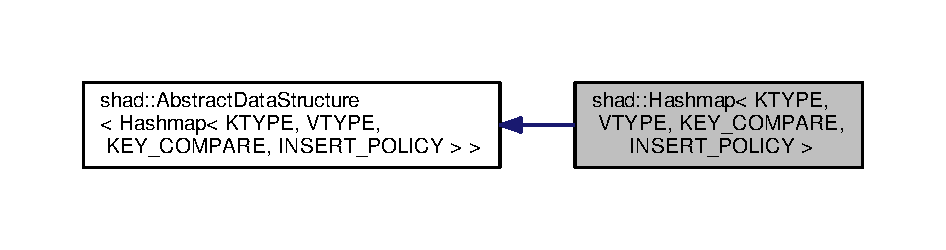
\includegraphics[width=350pt]{classshad_1_1Hashmap__inherit__graph}
\end{center}
\end{figure}


Collaboration diagram for shad\-:\-:Hashmap$<$ K\-T\-Y\-P\-E, V\-T\-Y\-P\-E, K\-E\-Y\-\_\-\-C\-O\-M\-P\-A\-R\-E, I\-N\-S\-E\-R\-T\-\_\-\-P\-O\-L\-I\-C\-Y $>$\-:
\nopagebreak
\begin{figure}[H]
\begin{center}
\leavevmode
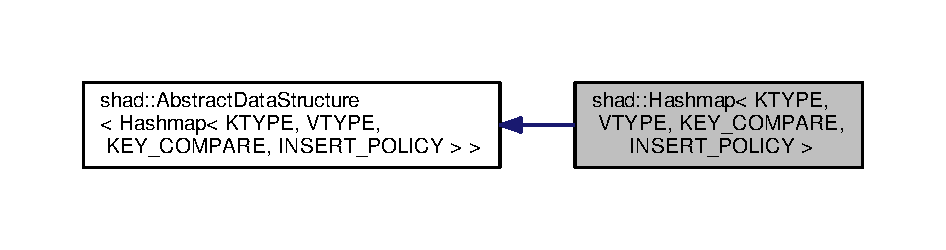
\includegraphics[width=350pt]{classshad_1_1Hashmap__coll__graph}
\end{center}
\end{figure}
\subsection*{Classes}
\begin{DoxyCompactItemize}
\item 
struct \hyperlink{structshad_1_1Hashmap_1_1EntryT}{Entry\-T}
\end{DoxyCompactItemize}
\subsection*{Public Types}
\begin{DoxyCompactItemize}
\item 
using \hyperlink{classshad_1_1Hashmap_ad8c0108347b59bcd19ccb8070a313dd8}{value\-\_\-type} = std\-::pair$<$ K\-T\-Y\-P\-E, V\-T\-Y\-P\-E $>$
\item 
using \hyperlink{classshad_1_1Hashmap_a8a56b050ace0e26454959cc45cdcb211}{Hmap\-T} = \hyperlink{classshad_1_1Hashmap}{Hashmap}$<$ K\-T\-Y\-P\-E, V\-T\-Y\-P\-E, K\-E\-Y\-\_\-\-C\-O\-M\-P\-A\-R\-E, I\-N\-S\-E\-R\-T\-\_\-\-P\-O\-L\-I\-C\-Y $>$
\item 
using \hyperlink{classshad_1_1Hashmap_aace37116c38330a70352a3081d0ec07e}{L\-Map\-T} = \hyperlink{classshad_1_1LocalHashmap}{Local\-Hashmap}$<$ K\-T\-Y\-P\-E, V\-T\-Y\-P\-E, K\-E\-Y\-\_\-\-C\-O\-M\-P\-A\-R\-E, I\-N\-S\-E\-R\-T\-\_\-\-P\-O\-L\-I\-C\-Y $>$
\item 
using \hyperlink{classshad_1_1Hashmap_a1f10a3b0cce639008b5b9444eb167f8b}{Object\-I\-D} = typename \hyperlink{classshad_1_1AbstractDataStructure}{Abstract\-Data\-Structure}$<$ \hyperlink{classshad_1_1Hashmap_a8a56b050ace0e26454959cc45cdcb211}{Hmap\-T} $>$\-::\hyperlink{classshad_1_1Hashmap_a1f10a3b0cce639008b5b9444eb167f8b}{Object\-I\-D}
\item 
using \hyperlink{classshad_1_1Hashmap_a5d013a5199b5745a1877b321af1b86ee}{Shad\-Hashmap\-Ptr} = typename \hyperlink{classshad_1_1AbstractDataStructure}{Abstract\-Data\-Structure}$<$ \hyperlink{classshad_1_1Hashmap_a8a56b050ace0e26454959cc45cdcb211}{Hmap\-T} $>$\-::\hyperlink{classshad_1_1AbstractDataStructure_a8bb29450966955c546d40421ce46316f}{Shared\-Ptr}
\item 
using \hyperlink{classshad_1_1Hashmap_a4603e48d3ad3a380abc888671e55bf01}{iterator} = \hyperlink{classshad_1_1map__iterator}{map\-\_\-iterator}$<$ \hyperlink{classshad_1_1Hashmap}{Hashmap}$<$ K\-T\-Y\-P\-E, V\-T\-Y\-P\-E, K\-E\-Y\-\_\-\-C\-O\-M\-P\-A\-R\-E, I\-N\-S\-E\-R\-T\-\_\-\-P\-O\-L\-I\-C\-Y $>$, std\-::pair$<$ K\-T\-Y\-P\-E, V\-T\-Y\-P\-E $>$, std\-::pair$<$ K\-T\-Y\-P\-E, V\-T\-Y\-P\-E $>$$>$
\item 
using \hyperlink{classshad_1_1Hashmap_a1f8a379c42bc2d4b67dcc9f519dc537e}{const\-\_\-iterator} = \hyperlink{classshad_1_1map__iterator}{map\-\_\-iterator}$<$ \hyperlink{classshad_1_1Hashmap}{Hashmap}$<$ K\-T\-Y\-P\-E, V\-T\-Y\-P\-E, K\-E\-Y\-\_\-\-C\-O\-M\-P\-A\-R\-E, I\-N\-S\-E\-R\-T\-\_\-\-P\-O\-L\-I\-C\-Y $>$, const std\-::pair$<$ K\-T\-Y\-P\-E, V\-T\-Y\-P\-E $>$, std\-::pair$<$ K\-T\-Y\-P\-E, V\-T\-Y\-P\-E $>$$>$
\item 
using \hyperlink{classshad_1_1Hashmap_abf95d16be9ba9060bff9fa591ece302f}{local\-\_\-iterator} = \hyperlink{classshad_1_1lmap__iterator}{lmap\-\_\-iterator}$<$ \hyperlink{classshad_1_1LocalHashmap}{Local\-Hashmap}$<$ K\-T\-Y\-P\-E, V\-T\-Y\-P\-E, K\-E\-Y\-\_\-\-C\-O\-M\-P\-A\-R\-E, I\-N\-S\-E\-R\-T\-\_\-\-P\-O\-L\-I\-C\-Y $>$, std\-::pair$<$ K\-T\-Y\-P\-E, V\-T\-Y\-P\-E $>$$>$
\item 
using \hyperlink{classshad_1_1Hashmap_afdf2dad495223a7d8bcec4256b591d89}{const\-\_\-local\-\_\-iterator} = \hyperlink{classshad_1_1lmap__iterator}{lmap\-\_\-iterator}$<$ \hyperlink{classshad_1_1LocalHashmap}{Local\-Hashmap}$<$ K\-T\-Y\-P\-E, V\-T\-Y\-P\-E, K\-E\-Y\-\_\-\-C\-O\-M\-P\-A\-R\-E, I\-N\-S\-E\-R\-T\-\_\-\-P\-O\-L\-I\-C\-Y $>$, const std\-::pair$<$ K\-T\-Y\-P\-E, V\-T\-Y\-P\-E $>$$>$
\item 
using \hyperlink{classshad_1_1Hashmap_abe8958800566729b4fe4b46d0e5d8f70}{Buffers\-Vector} = typename impl\-::\-Buffers\-Vector$<$ \hyperlink{structshad_1_1Hashmap_1_1EntryT}{Entry\-T}, \hyperlink{classshad_1_1Hashmap_a8a56b050ace0e26454959cc45cdcb211}{Hmap\-T} $>$
\item 
using \hyperlink{classshad_1_1Hashmap_acc8ac68502c6c886d18d660e907fef0a}{Lookup\-Result} = typename \hyperlink{classshad_1_1LocalHashmap}{Local\-Hashmap}$<$ K\-T\-Y\-P\-E, V\-T\-Y\-P\-E, K\-E\-Y\-\_\-\-C\-O\-M\-P\-A\-R\-E $>$\-::\hyperlink{classshad_1_1Hashmap_acc8ac68502c6c886d18d660e907fef0a}{Lookup\-Result}
\end{DoxyCompactItemize}
\subsection*{Public Member Functions}
\begin{DoxyCompactItemize}
\item 
\hyperlink{classshad_1_1Hashmap_a1f10a3b0cce639008b5b9444eb167f8b}{Object\-I\-D} \hyperlink{classshad_1_1Hashmap_a7a7242cd82188b05280e4f8faaeac387}{Get\-Global\-I\-D} () const 
\begin{DoxyCompactList}\small\item\em Getter of the Global Identifier. \end{DoxyCompactList}\item 
size\-\_\-t \hyperlink{classshad_1_1Hashmap_ae05da08d72f0a2097a64603f49cc91ac}{Size} () const 
\begin{DoxyCompactList}\small\item\em Overall size of the hashmap (number of entries). \end{DoxyCompactList}\item 
void \hyperlink{classshad_1_1Hashmap_af3f0622044572a21c74f192714065f5f}{Insert} (const K\-T\-Y\-P\-E \&key, const V\-T\-Y\-P\-E \&value)
\begin{DoxyCompactList}\small\item\em Insert a key-\/value pair in the hashmap. \end{DoxyCompactList}\item 
void \hyperlink{classshad_1_1Hashmap_a6cfddc1040192ee87e5c41f443e6557d}{Async\-Insert} (\hyperlink{classshad_1_1rt_1_1Handle}{rt\-::\-Handle} \&handle, const K\-T\-Y\-P\-E \&key, const V\-T\-Y\-P\-E \&value)
\begin{DoxyCompactList}\small\item\em Asynchronously Insert a key-\/value pair in the hashmap. \end{DoxyCompactList}\item 
void \hyperlink{classshad_1_1Hashmap_a94e4c630fc430e83776f8a34fcae06c2}{Buffered\-Insert} (const K\-T\-Y\-P\-E \&key, const V\-T\-Y\-P\-E \&value)
\begin{DoxyCompactList}\small\item\em Buffered Insert method. Inserts a key-\/value pair, using aggregation buffers. \end{DoxyCompactList}\item 
void \hyperlink{classshad_1_1Hashmap_a81d82387ec408ec61db465e60401c77a}{Buffered\-Async\-Insert} (\hyperlink{classshad_1_1rt_1_1Handle}{rt\-::\-Handle} \&handle, const K\-T\-Y\-P\-E \&key, const V\-T\-Y\-P\-E \&value)
\begin{DoxyCompactList}\small\item\em Asynchronous Buffered Insert method. Asynchronously inserts a key-\/value pair, using aggregation buffers. \end{DoxyCompactList}\item 
void \hyperlink{classshad_1_1Hashmap_a002531ab15c552400f95ec80029d4eed}{Wait\-For\-Buffered\-Insert} ()
\begin{DoxyCompactList}\small\item\em Finalize method for buffered insertions. \end{DoxyCompactList}\item 
void \hyperlink{classshad_1_1Hashmap_ad93d311ba86a6a7d80120f67d846dbd5}{Erase} (const K\-T\-Y\-P\-E \&key)
\begin{DoxyCompactList}\small\item\em Remove a key-\/value pair from the hashmap. \end{DoxyCompactList}\item 
void \hyperlink{classshad_1_1Hashmap_aff16ee975fc59681c4ce7e9ae79b4125}{Async\-Erase} (\hyperlink{classshad_1_1rt_1_1Handle}{rt\-::\-Handle} \&handle, const K\-T\-Y\-P\-E \&key)
\begin{DoxyCompactList}\small\item\em Asynchronously remove a key-\/value pair from the hashmap. \end{DoxyCompactList}\item 
void \hyperlink{classshad_1_1Hashmap_a708b4f1033b3119ed2cc2afd0d469341}{Clear} ()
\begin{DoxyCompactList}\small\item\em Clear the content of the hashmap. \end{DoxyCompactList}\item 
bool \hyperlink{classshad_1_1Hashmap_a86cce815ed1c4854c36958611cc32377}{Lookup} (const K\-T\-Y\-P\-E \&key, V\-T\-Y\-P\-E $\ast$res)
\begin{DoxyCompactList}\small\item\em Get the value associated to a key. \end{DoxyCompactList}\item 
void \hyperlink{classshad_1_1Hashmap_aeca796c945726ce7ab4b67e1add6bb1f}{Async\-Lookup} (\hyperlink{classshad_1_1rt_1_1Handle}{rt\-::\-Handle} \&handle, const K\-T\-Y\-P\-E \&key, \hyperlink{classshad_1_1Hashmap_acc8ac68502c6c886d18d660e907fef0a}{Lookup\-Result} $\ast$res)
\begin{DoxyCompactList}\small\item\em Asynchronous lookup method. \end{DoxyCompactList}\item 
{\footnotesize template$<$typename Apply\-Fun\-T , typename... Args$>$ }\\void \hyperlink{classshad_1_1Hashmap_ad8cca9577908ecd19463eb6e89d1df8e}{Apply} (const K\-T\-Y\-P\-E \&key, Apply\-Fun\-T \&\&function, Args \&...args)
\begin{DoxyCompactList}\small\item\em Apply a user-\/defined function to a key-\/value pair. \end{DoxyCompactList}\item 
{\footnotesize template$<$typename Apply\-Fun\-T , typename... Args$>$ }\\void \hyperlink{classshad_1_1Hashmap_aa2e494d7ecb711f9e8a1f077fa0aba6d}{Async\-Apply} (\hyperlink{classshad_1_1rt_1_1Handle}{rt\-::\-Handle} \&handle, const K\-T\-Y\-P\-E \&key, Apply\-Fun\-T \&\&function, Args \&...args)
\begin{DoxyCompactList}\small\item\em Asynchronously apply a user-\/defined function to a key-\/value pair. \end{DoxyCompactList}\item 
{\footnotesize template$<$typename Apply\-Fun\-T , typename... Args$>$ }\\void \hyperlink{classshad_1_1Hashmap_a8013caa5b8fd66516bcf24d2eabf5f61}{For\-Each\-Entry} (Apply\-Fun\-T \&\&function, Args \&...args)
\begin{DoxyCompactList}\small\item\em Apply a user-\/defined function to each key-\/value pair. \end{DoxyCompactList}\item 
{\footnotesize template$<$typename Apply\-Fun\-T , typename... Args$>$ }\\void \hyperlink{classshad_1_1Hashmap_a041eacf973eaadac4a710997ec22cb48}{Async\-For\-Each\-Entry} (\hyperlink{classshad_1_1rt_1_1Handle}{rt\-::\-Handle} \&handle, Apply\-Fun\-T \&\&function, Args \&...args)
\begin{DoxyCompactList}\small\item\em Asynchronously apply a user-\/defined function to each key-\/value pair. \end{DoxyCompactList}\item 
{\footnotesize template$<$typename Apply\-Fun\-T , typename... Args$>$ }\\void \hyperlink{classshad_1_1Hashmap_afd8abe4f63a6570b29578dae3b449249}{For\-Each\-Key} (Apply\-Fun\-T \&\&function, Args \&...args)
\begin{DoxyCompactList}\small\item\em Apply a user-\/defined function to each key. \end{DoxyCompactList}\item 
{\footnotesize template$<$typename Apply\-Fun\-T , typename... Args$>$ }\\void \hyperlink{classshad_1_1Hashmap_acd1166f6dd5ad1f9f3748ea45b596860}{Async\-For\-Each\-Key} (\hyperlink{classshad_1_1rt_1_1Handle}{rt\-::\-Handle} \&handle, Apply\-Fun\-T \&\&function, Args \&...args)
\begin{DoxyCompactList}\small\item\em Asynchronously apply a user-\/defined function to each key. \end{DoxyCompactList}\item 
void \hyperlink{classshad_1_1Hashmap_aee2b37787d771a453bfe49a85e352e3e}{Print\-All\-Entries} ()
\item 
void \hyperlink{classshad_1_1Hashmap_a313c1401e0dd0cc51cfc750a740f3772}{Buffer\-Entry\-Insert} (const \hyperlink{structshad_1_1Hashmap_1_1EntryT}{Entry\-T} \&entry)
\item 
\hyperlink{classshad_1_1Hashmap_a4603e48d3ad3a380abc888671e55bf01}{iterator} \hyperlink{classshad_1_1Hashmap_a8f4a24ff42fd6f6c3394a352169bccb9}{begin} ()
\item 
\hyperlink{classshad_1_1Hashmap_a4603e48d3ad3a380abc888671e55bf01}{iterator} \hyperlink{classshad_1_1Hashmap_a72709bee83695661dbd0a43699cd1833}{end} ()
\item 
\hyperlink{classshad_1_1Hashmap_a1f8a379c42bc2d4b67dcc9f519dc537e}{const\-\_\-iterator} \hyperlink{classshad_1_1Hashmap_aa014bed8d66b4adb7274687b9074cc53}{cbegin} ()
\item 
\hyperlink{classshad_1_1Hashmap_a1f8a379c42bc2d4b67dcc9f519dc537e}{const\-\_\-iterator} \hyperlink{classshad_1_1Hashmap_a75006495ce7c58a32c5724cae27944ed}{cend} ()
\item 
\hyperlink{classshad_1_1Hashmap_abf95d16be9ba9060bff9fa591ece302f}{local\-\_\-iterator} \hyperlink{classshad_1_1Hashmap_a4706991a9277cc89fcd154bf73025183}{local\-\_\-begin} ()
\item 
\hyperlink{classshad_1_1Hashmap_abf95d16be9ba9060bff9fa591ece302f}{local\-\_\-iterator} \hyperlink{classshad_1_1Hashmap_a6fff153fc13d2d3c3337ac0dfa594b28}{local\-\_\-end} ()
\item 
\hyperlink{classshad_1_1Hashmap_afdf2dad495223a7d8bcec4256b591d89}{const\-\_\-local\-\_\-iterator} \hyperlink{classshad_1_1Hashmap_a04a14f79c423b6bef9fba77f642be9b6}{clocal\-\_\-begin} ()
\item 
\hyperlink{classshad_1_1Hashmap_afdf2dad495223a7d8bcec4256b591d89}{const\-\_\-local\-\_\-iterator} \hyperlink{classshad_1_1Hashmap_a41013ec16375b3de1af140c8f2e54627}{clocal\-\_\-end} ()
\end{DoxyCompactItemize}
\subsection*{Static Public Member Functions}
\begin{DoxyCompactItemize}
\item 
static \hyperlink{classshad_1_1Hashmap_a5d013a5199b5745a1877b321af1b86ee}{Shad\-Hashmap\-Ptr} \hyperlink{classshad_1_1Hashmap_a304075c88faf0d3eff16c8a6b380138c}{Create} (const size\-\_\-t num\-Entries)
\begin{DoxyCompactList}\small\item\em Create method. \end{DoxyCompactList}\end{DoxyCompactItemize}
\subsection*{Protected Member Functions}
\begin{DoxyCompactItemize}
\item 
\hyperlink{classshad_1_1Hashmap_a8b729b8e8fe6186be91856998b29ef70}{Hashmap} (\hyperlink{classshad_1_1Hashmap_a1f10a3b0cce639008b5b9444eb167f8b}{Object\-I\-D} oid, const size\-\_\-t num\-Entries)
\end{DoxyCompactItemize}
\subsection*{Friends}
\begin{DoxyCompactItemize}
\item 
{\footnotesize template$<$typename $>$ }\\class \hyperlink{classshad_1_1Hashmap_ab18afa4496cc863ddc11bab94b2adf57}{Abstract\-Data\-Structure}
\item 
class \hyperlink{classshad_1_1Hashmap_a9f6643e9369026a8c41dff0b7bca9e4b}{map\-\_\-iterator$<$ Hashmap$<$ K\-T\-Y\-P\-E, V\-T\-Y\-P\-E, K\-E\-Y\-\_\-\-C\-O\-M\-P\-A\-R\-E, I\-N\-S\-E\-R\-T\-\_\-\-P\-O\-L\-I\-C\-Y $>$, std\-::pair$<$ K\-T\-Y\-P\-E, V\-T\-Y\-P\-E $>$, std\-::pair$<$ K\-T\-Y\-P\-E, V\-T\-Y\-P\-E $>$ $>$}
\item 
class \hyperlink{classshad_1_1Hashmap_a901992501a956914085e608ae303244f}{map\-\_\-iterator$<$ Hashmap$<$ K\-T\-Y\-P\-E, V\-T\-Y\-P\-E, K\-E\-Y\-\_\-\-C\-O\-M\-P\-A\-R\-E, I\-N\-S\-E\-R\-T\-\_\-\-P\-O\-L\-I\-C\-Y $>$, const std\-::pair$<$ K\-T\-Y\-P\-E, V\-T\-Y\-P\-E $>$, std\-::pair$<$ K\-T\-Y\-P\-E, V\-T\-Y\-P\-E $>$ $>$}
\end{DoxyCompactItemize}
\subsection*{Additional Inherited Members}


\subsection{Detailed Description}
\subsubsection*{template$<$typename K\-T\-Y\-P\-E, typename V\-T\-Y\-P\-E, typename K\-E\-Y\-\_\-\-C\-O\-M\-P\-A\-R\-E = Mem\-Cmp$<$\-K\-T\-Y\-P\-E$>$, typename I\-N\-S\-E\-R\-T\-\_\-\-P\-O\-L\-I\-C\-Y = Overwriter$<$\-V\-T\-Y\-P\-E$>$$>$class shad\-::\-Hashmap$<$ K\-T\-Y\-P\-E, V\-T\-Y\-P\-E, K\-E\-Y\-\_\-\-C\-O\-M\-P\-A\-R\-E, I\-N\-S\-E\-R\-T\-\_\-\-P\-O\-L\-I\-C\-Y $>$}

The \hyperlink{classshad_1_1Hashmap}{Hashmap} data structure. 

S\-H\-A\-D's \hyperlink{classshad_1_1Hashmap}{Hashmap} is a distributed, thread-\/safe, associative container. 
\begin{DoxyTemplParams}{Template Parameters}
{\em K\-T\-Y\-P\-E} & type of the hashmap keys. \\
\hline
{\em V\-T\-Y\-P\-E} & type of the hashmap values. \\
\hline
{\em K\-E\-Y\-\_\-\-C\-O\-M\-P\-A\-R\-E} & key comparison function; default is Mem\-Cmp$<$\-K\-T\-Y\-P\-E$>$. \\
\hline
\end{DoxyTemplParams}
\begin{DoxyWarning}{Warning}
obects of type K\-T\-Y\-P\-E and V\-T\-Y\-P\-E need to be trivially copiable. 
\end{DoxyWarning}

\begin{DoxyTemplParams}{Template Parameters}
{\em I\-N\-S\-E\-R\-T\-\_\-\-P\-O\-L\-I\-C\-Y} & insertion policy; default is overwrite (i.\-e. insertions overwrite previous values associated to the same key, if any). \\
\hline
\end{DoxyTemplParams}


\subsection{Member Typedef Documentation}
\hypertarget{classshad_1_1Hashmap_abe8958800566729b4fe4b46d0e5d8f70}{\index{shad\-::\-Hashmap@{shad\-::\-Hashmap}!Buffers\-Vector@{Buffers\-Vector}}
\index{Buffers\-Vector@{Buffers\-Vector}!shad::Hashmap@{shad\-::\-Hashmap}}
\subsubsection[{Buffers\-Vector}]{\setlength{\rightskip}{0pt plus 5cm}template$<$typename K\-T\-Y\-P\-E , typename V\-T\-Y\-P\-E , typename K\-E\-Y\-\_\-\-C\-O\-M\-P\-A\-R\-E  = Mem\-Cmp$<$\-K\-T\-Y\-P\-E$>$, typename I\-N\-S\-E\-R\-T\-\_\-\-P\-O\-L\-I\-C\-Y  = Overwriter$<$\-V\-T\-Y\-P\-E$>$$>$ using {\bf shad\-::\-Hashmap}$<$ K\-T\-Y\-P\-E, V\-T\-Y\-P\-E, K\-E\-Y\-\_\-\-C\-O\-M\-P\-A\-R\-E, I\-N\-S\-E\-R\-T\-\_\-\-P\-O\-L\-I\-C\-Y $>$\-::{\bf Buffers\-Vector} =  typename impl\-::\-Buffers\-Vector$<${\bf Entry\-T}, {\bf Hmap\-T}$>$}}\label{classshad_1_1Hashmap_abe8958800566729b4fe4b46d0e5d8f70}
\hypertarget{classshad_1_1Hashmap_a1f8a379c42bc2d4b67dcc9f519dc537e}{\index{shad\-::\-Hashmap@{shad\-::\-Hashmap}!const\-\_\-iterator@{const\-\_\-iterator}}
\index{const\-\_\-iterator@{const\-\_\-iterator}!shad::Hashmap@{shad\-::\-Hashmap}}
\subsubsection[{const\-\_\-iterator}]{\setlength{\rightskip}{0pt plus 5cm}template$<$typename K\-T\-Y\-P\-E , typename V\-T\-Y\-P\-E , typename K\-E\-Y\-\_\-\-C\-O\-M\-P\-A\-R\-E  = Mem\-Cmp$<$\-K\-T\-Y\-P\-E$>$, typename I\-N\-S\-E\-R\-T\-\_\-\-P\-O\-L\-I\-C\-Y  = Overwriter$<$\-V\-T\-Y\-P\-E$>$$>$ using {\bf shad\-::\-Hashmap}$<$ K\-T\-Y\-P\-E, V\-T\-Y\-P\-E, K\-E\-Y\-\_\-\-C\-O\-M\-P\-A\-R\-E, I\-N\-S\-E\-R\-T\-\_\-\-P\-O\-L\-I\-C\-Y $>$\-::{\bf const\-\_\-iterator} =  {\bf map\-\_\-iterator}$<${\bf Hashmap}$<$K\-T\-Y\-P\-E, V\-T\-Y\-P\-E, K\-E\-Y\-\_\-\-C\-O\-M\-P\-A\-R\-E, I\-N\-S\-E\-R\-T\-\_\-\-P\-O\-L\-I\-C\-Y$>$, const std\-::pair$<$K\-T\-Y\-P\-E, V\-T\-Y\-P\-E$>$, std\-::pair$<$K\-T\-Y\-P\-E, V\-T\-Y\-P\-E$>$$>$}}\label{classshad_1_1Hashmap_a1f8a379c42bc2d4b67dcc9f519dc537e}
\hypertarget{classshad_1_1Hashmap_afdf2dad495223a7d8bcec4256b591d89}{\index{shad\-::\-Hashmap@{shad\-::\-Hashmap}!const\-\_\-local\-\_\-iterator@{const\-\_\-local\-\_\-iterator}}
\index{const\-\_\-local\-\_\-iterator@{const\-\_\-local\-\_\-iterator}!shad::Hashmap@{shad\-::\-Hashmap}}
\subsubsection[{const\-\_\-local\-\_\-iterator}]{\setlength{\rightskip}{0pt plus 5cm}template$<$typename K\-T\-Y\-P\-E , typename V\-T\-Y\-P\-E , typename K\-E\-Y\-\_\-\-C\-O\-M\-P\-A\-R\-E  = Mem\-Cmp$<$\-K\-T\-Y\-P\-E$>$, typename I\-N\-S\-E\-R\-T\-\_\-\-P\-O\-L\-I\-C\-Y  = Overwriter$<$\-V\-T\-Y\-P\-E$>$$>$ using {\bf shad\-::\-Hashmap}$<$ K\-T\-Y\-P\-E, V\-T\-Y\-P\-E, K\-E\-Y\-\_\-\-C\-O\-M\-P\-A\-R\-E, I\-N\-S\-E\-R\-T\-\_\-\-P\-O\-L\-I\-C\-Y $>$\-::{\bf const\-\_\-local\-\_\-iterator} =  {\bf lmap\-\_\-iterator}$<${\bf Local\-Hashmap}$<$K\-T\-Y\-P\-E, V\-T\-Y\-P\-E, K\-E\-Y\-\_\-\-C\-O\-M\-P\-A\-R\-E, I\-N\-S\-E\-R\-T\-\_\-\-P\-O\-L\-I\-C\-Y$>$, const std\-::pair$<$K\-T\-Y\-P\-E, V\-T\-Y\-P\-E$>$$>$}}\label{classshad_1_1Hashmap_afdf2dad495223a7d8bcec4256b591d89}
\hypertarget{classshad_1_1Hashmap_a8a56b050ace0e26454959cc45cdcb211}{\index{shad\-::\-Hashmap@{shad\-::\-Hashmap}!Hmap\-T@{Hmap\-T}}
\index{Hmap\-T@{Hmap\-T}!shad::Hashmap@{shad\-::\-Hashmap}}
\subsubsection[{Hmap\-T}]{\setlength{\rightskip}{0pt plus 5cm}template$<$typename K\-T\-Y\-P\-E , typename V\-T\-Y\-P\-E , typename K\-E\-Y\-\_\-\-C\-O\-M\-P\-A\-R\-E  = Mem\-Cmp$<$\-K\-T\-Y\-P\-E$>$, typename I\-N\-S\-E\-R\-T\-\_\-\-P\-O\-L\-I\-C\-Y  = Overwriter$<$\-V\-T\-Y\-P\-E$>$$>$ using {\bf shad\-::\-Hashmap}$<$ K\-T\-Y\-P\-E, V\-T\-Y\-P\-E, K\-E\-Y\-\_\-\-C\-O\-M\-P\-A\-R\-E, I\-N\-S\-E\-R\-T\-\_\-\-P\-O\-L\-I\-C\-Y $>$\-::{\bf Hmap\-T} =  {\bf Hashmap}$<$K\-T\-Y\-P\-E, V\-T\-Y\-P\-E, K\-E\-Y\-\_\-\-C\-O\-M\-P\-A\-R\-E, I\-N\-S\-E\-R\-T\-\_\-\-P\-O\-L\-I\-C\-Y$>$}}\label{classshad_1_1Hashmap_a8a56b050ace0e26454959cc45cdcb211}
\hypertarget{classshad_1_1Hashmap_a4603e48d3ad3a380abc888671e55bf01}{\index{shad\-::\-Hashmap@{shad\-::\-Hashmap}!iterator@{iterator}}
\index{iterator@{iterator}!shad::Hashmap@{shad\-::\-Hashmap}}
\subsubsection[{iterator}]{\setlength{\rightskip}{0pt plus 5cm}template$<$typename K\-T\-Y\-P\-E , typename V\-T\-Y\-P\-E , typename K\-E\-Y\-\_\-\-C\-O\-M\-P\-A\-R\-E  = Mem\-Cmp$<$\-K\-T\-Y\-P\-E$>$, typename I\-N\-S\-E\-R\-T\-\_\-\-P\-O\-L\-I\-C\-Y  = Overwriter$<$\-V\-T\-Y\-P\-E$>$$>$ using {\bf shad\-::\-Hashmap}$<$ K\-T\-Y\-P\-E, V\-T\-Y\-P\-E, K\-E\-Y\-\_\-\-C\-O\-M\-P\-A\-R\-E, I\-N\-S\-E\-R\-T\-\_\-\-P\-O\-L\-I\-C\-Y $>$\-::{\bf iterator} =  {\bf map\-\_\-iterator}$<${\bf Hashmap}$<$K\-T\-Y\-P\-E, V\-T\-Y\-P\-E, K\-E\-Y\-\_\-\-C\-O\-M\-P\-A\-R\-E, I\-N\-S\-E\-R\-T\-\_\-\-P\-O\-L\-I\-C\-Y$>$, std\-::pair$<$K\-T\-Y\-P\-E, V\-T\-Y\-P\-E$>$, std\-::pair$<$K\-T\-Y\-P\-E, V\-T\-Y\-P\-E$>$$>$}}\label{classshad_1_1Hashmap_a4603e48d3ad3a380abc888671e55bf01}
\hypertarget{classshad_1_1Hashmap_aace37116c38330a70352a3081d0ec07e}{\index{shad\-::\-Hashmap@{shad\-::\-Hashmap}!L\-Map\-T@{L\-Map\-T}}
\index{L\-Map\-T@{L\-Map\-T}!shad::Hashmap@{shad\-::\-Hashmap}}
\subsubsection[{L\-Map\-T}]{\setlength{\rightskip}{0pt plus 5cm}template$<$typename K\-T\-Y\-P\-E , typename V\-T\-Y\-P\-E , typename K\-E\-Y\-\_\-\-C\-O\-M\-P\-A\-R\-E  = Mem\-Cmp$<$\-K\-T\-Y\-P\-E$>$, typename I\-N\-S\-E\-R\-T\-\_\-\-P\-O\-L\-I\-C\-Y  = Overwriter$<$\-V\-T\-Y\-P\-E$>$$>$ using {\bf shad\-::\-Hashmap}$<$ K\-T\-Y\-P\-E, V\-T\-Y\-P\-E, K\-E\-Y\-\_\-\-C\-O\-M\-P\-A\-R\-E, I\-N\-S\-E\-R\-T\-\_\-\-P\-O\-L\-I\-C\-Y $>$\-::{\bf L\-Map\-T} =  {\bf Local\-Hashmap}$<$K\-T\-Y\-P\-E, V\-T\-Y\-P\-E, K\-E\-Y\-\_\-\-C\-O\-M\-P\-A\-R\-E, I\-N\-S\-E\-R\-T\-\_\-\-P\-O\-L\-I\-C\-Y$>$}}\label{classshad_1_1Hashmap_aace37116c38330a70352a3081d0ec07e}
\hypertarget{classshad_1_1Hashmap_abf95d16be9ba9060bff9fa591ece302f}{\index{shad\-::\-Hashmap@{shad\-::\-Hashmap}!local\-\_\-iterator@{local\-\_\-iterator}}
\index{local\-\_\-iterator@{local\-\_\-iterator}!shad::Hashmap@{shad\-::\-Hashmap}}
\subsubsection[{local\-\_\-iterator}]{\setlength{\rightskip}{0pt plus 5cm}template$<$typename K\-T\-Y\-P\-E , typename V\-T\-Y\-P\-E , typename K\-E\-Y\-\_\-\-C\-O\-M\-P\-A\-R\-E  = Mem\-Cmp$<$\-K\-T\-Y\-P\-E$>$, typename I\-N\-S\-E\-R\-T\-\_\-\-P\-O\-L\-I\-C\-Y  = Overwriter$<$\-V\-T\-Y\-P\-E$>$$>$ using {\bf shad\-::\-Hashmap}$<$ K\-T\-Y\-P\-E, V\-T\-Y\-P\-E, K\-E\-Y\-\_\-\-C\-O\-M\-P\-A\-R\-E, I\-N\-S\-E\-R\-T\-\_\-\-P\-O\-L\-I\-C\-Y $>$\-::{\bf local\-\_\-iterator} =  {\bf lmap\-\_\-iterator}$<${\bf Local\-Hashmap}$<$K\-T\-Y\-P\-E, V\-T\-Y\-P\-E, K\-E\-Y\-\_\-\-C\-O\-M\-P\-A\-R\-E, I\-N\-S\-E\-R\-T\-\_\-\-P\-O\-L\-I\-C\-Y$>$, std\-::pair$<$K\-T\-Y\-P\-E, V\-T\-Y\-P\-E$>$$>$}}\label{classshad_1_1Hashmap_abf95d16be9ba9060bff9fa591ece302f}
\hypertarget{classshad_1_1Hashmap_acc8ac68502c6c886d18d660e907fef0a}{\index{shad\-::\-Hashmap@{shad\-::\-Hashmap}!Lookup\-Result@{Lookup\-Result}}
\index{Lookup\-Result@{Lookup\-Result}!shad::Hashmap@{shad\-::\-Hashmap}}
\subsubsection[{Lookup\-Result}]{\setlength{\rightskip}{0pt plus 5cm}template$<$typename K\-T\-Y\-P\-E , typename V\-T\-Y\-P\-E , typename K\-E\-Y\-\_\-\-C\-O\-M\-P\-A\-R\-E  = Mem\-Cmp$<$\-K\-T\-Y\-P\-E$>$, typename I\-N\-S\-E\-R\-T\-\_\-\-P\-O\-L\-I\-C\-Y  = Overwriter$<$\-V\-T\-Y\-P\-E$>$$>$ using {\bf shad\-::\-Hashmap}$<$ K\-T\-Y\-P\-E, V\-T\-Y\-P\-E, K\-E\-Y\-\_\-\-C\-O\-M\-P\-A\-R\-E, I\-N\-S\-E\-R\-T\-\_\-\-P\-O\-L\-I\-C\-Y $>$\-::{\bf Lookup\-Result} =  typename {\bf Local\-Hashmap}$<$K\-T\-Y\-P\-E, V\-T\-Y\-P\-E, K\-E\-Y\-\_\-\-C\-O\-M\-P\-A\-R\-E$>$\-::{\bf Lookup\-Result}}}\label{classshad_1_1Hashmap_acc8ac68502c6c886d18d660e907fef0a}
\hypertarget{classshad_1_1Hashmap_a1f10a3b0cce639008b5b9444eb167f8b}{\index{shad\-::\-Hashmap@{shad\-::\-Hashmap}!Object\-I\-D@{Object\-I\-D}}
\index{Object\-I\-D@{Object\-I\-D}!shad::Hashmap@{shad\-::\-Hashmap}}
\subsubsection[{Object\-I\-D}]{\setlength{\rightskip}{0pt plus 5cm}template$<$typename K\-T\-Y\-P\-E , typename V\-T\-Y\-P\-E , typename K\-E\-Y\-\_\-\-C\-O\-M\-P\-A\-R\-E  = Mem\-Cmp$<$\-K\-T\-Y\-P\-E$>$, typename I\-N\-S\-E\-R\-T\-\_\-\-P\-O\-L\-I\-C\-Y  = Overwriter$<$\-V\-T\-Y\-P\-E$>$$>$ using {\bf shad\-::\-Hashmap}$<$ K\-T\-Y\-P\-E, V\-T\-Y\-P\-E, K\-E\-Y\-\_\-\-C\-O\-M\-P\-A\-R\-E, I\-N\-S\-E\-R\-T\-\_\-\-P\-O\-L\-I\-C\-Y $>$\-::{\bf Object\-I\-D} =  typename {\bf Abstract\-Data\-Structure}$<${\bf Hmap\-T}$>$\-::{\bf Object\-I\-D}}}\label{classshad_1_1Hashmap_a1f10a3b0cce639008b5b9444eb167f8b}
\hypertarget{classshad_1_1Hashmap_a5d013a5199b5745a1877b321af1b86ee}{\index{shad\-::\-Hashmap@{shad\-::\-Hashmap}!Shad\-Hashmap\-Ptr@{Shad\-Hashmap\-Ptr}}
\index{Shad\-Hashmap\-Ptr@{Shad\-Hashmap\-Ptr}!shad::Hashmap@{shad\-::\-Hashmap}}
\subsubsection[{Shad\-Hashmap\-Ptr}]{\setlength{\rightskip}{0pt plus 5cm}template$<$typename K\-T\-Y\-P\-E , typename V\-T\-Y\-P\-E , typename K\-E\-Y\-\_\-\-C\-O\-M\-P\-A\-R\-E  = Mem\-Cmp$<$\-K\-T\-Y\-P\-E$>$, typename I\-N\-S\-E\-R\-T\-\_\-\-P\-O\-L\-I\-C\-Y  = Overwriter$<$\-V\-T\-Y\-P\-E$>$$>$ using {\bf shad\-::\-Hashmap}$<$ K\-T\-Y\-P\-E, V\-T\-Y\-P\-E, K\-E\-Y\-\_\-\-C\-O\-M\-P\-A\-R\-E, I\-N\-S\-E\-R\-T\-\_\-\-P\-O\-L\-I\-C\-Y $>$\-::{\bf Shad\-Hashmap\-Ptr} =  typename {\bf Abstract\-Data\-Structure}$<${\bf Hmap\-T}$>$\-::{\bf Shared\-Ptr}}}\label{classshad_1_1Hashmap_a5d013a5199b5745a1877b321af1b86ee}
\hypertarget{classshad_1_1Hashmap_ad8c0108347b59bcd19ccb8070a313dd8}{\index{shad\-::\-Hashmap@{shad\-::\-Hashmap}!value\-\_\-type@{value\-\_\-type}}
\index{value\-\_\-type@{value\-\_\-type}!shad::Hashmap@{shad\-::\-Hashmap}}
\subsubsection[{value\-\_\-type}]{\setlength{\rightskip}{0pt plus 5cm}template$<$typename K\-T\-Y\-P\-E , typename V\-T\-Y\-P\-E , typename K\-E\-Y\-\_\-\-C\-O\-M\-P\-A\-R\-E  = Mem\-Cmp$<$\-K\-T\-Y\-P\-E$>$, typename I\-N\-S\-E\-R\-T\-\_\-\-P\-O\-L\-I\-C\-Y  = Overwriter$<$\-V\-T\-Y\-P\-E$>$$>$ using {\bf shad\-::\-Hashmap}$<$ K\-T\-Y\-P\-E, V\-T\-Y\-P\-E, K\-E\-Y\-\_\-\-C\-O\-M\-P\-A\-R\-E, I\-N\-S\-E\-R\-T\-\_\-\-P\-O\-L\-I\-C\-Y $>$\-::{\bf value\-\_\-type} =  std\-::pair$<$K\-T\-Y\-P\-E, V\-T\-Y\-P\-E$>$}}\label{classshad_1_1Hashmap_ad8c0108347b59bcd19ccb8070a313dd8}


\subsection{Constructor \& Destructor Documentation}
\hypertarget{classshad_1_1Hashmap_a8b729b8e8fe6186be91856998b29ef70}{\index{shad\-::\-Hashmap@{shad\-::\-Hashmap}!Hashmap@{Hashmap}}
\index{Hashmap@{Hashmap}!shad::Hashmap@{shad\-::\-Hashmap}}
\subsubsection[{Hashmap}]{\setlength{\rightskip}{0pt plus 5cm}template$<$typename K\-T\-Y\-P\-E , typename V\-T\-Y\-P\-E , typename K\-E\-Y\-\_\-\-C\-O\-M\-P\-A\-R\-E  = Mem\-Cmp$<$\-K\-T\-Y\-P\-E$>$, typename I\-N\-S\-E\-R\-T\-\_\-\-P\-O\-L\-I\-C\-Y  = Overwriter$<$\-V\-T\-Y\-P\-E$>$$>$ {\bf shad\-::\-Hashmap}$<$ K\-T\-Y\-P\-E, V\-T\-Y\-P\-E, K\-E\-Y\-\_\-\-C\-O\-M\-P\-A\-R\-E, I\-N\-S\-E\-R\-T\-\_\-\-P\-O\-L\-I\-C\-Y $>$\-::{\bf Hashmap} (
\begin{DoxyParamCaption}
\item[{{\bf Object\-I\-D}}]{oid, }
\item[{const size\-\_\-t}]{num\-Entries}
\end{DoxyParamCaption}
)\hspace{0.3cm}{\ttfamily [inline]}, {\ttfamily [protected]}}}\label{classshad_1_1Hashmap_a8b729b8e8fe6186be91856998b29ef70}


\subsection{Member Function Documentation}
\hypertarget{classshad_1_1Hashmap_ad8cca9577908ecd19463eb6e89d1df8e}{\index{shad\-::\-Hashmap@{shad\-::\-Hashmap}!Apply@{Apply}}
\index{Apply@{Apply}!shad::Hashmap@{shad\-::\-Hashmap}}
\subsubsection[{Apply}]{\setlength{\rightskip}{0pt plus 5cm}template$<$typename K\-T\-Y\-P\-E , typename V\-T\-Y\-P\-E , typename K\-E\-Y\-\_\-\-C\-O\-M\-P\-A\-R\-E , typename I\-N\-S\-E\-R\-T\-\_\-\-P\-O\-L\-I\-C\-Y $>$ template$<$typename Apply\-Fun\-T , typename... Args$>$ void {\bf shad\-::\-Hashmap}$<$ K\-T\-Y\-P\-E, V\-T\-Y\-P\-E, K\-E\-Y\-\_\-\-C\-O\-M\-P\-A\-R\-E, I\-N\-S\-E\-R\-T\-\_\-\-P\-O\-L\-I\-C\-Y $>$\-::Apply (
\begin{DoxyParamCaption}
\item[{const K\-T\-Y\-P\-E \&}]{key, }
\item[{Apply\-Fun\-T \&\&}]{function, }
\item[{Args \&...}]{args}
\end{DoxyParamCaption}
)}}\label{classshad_1_1Hashmap_ad8cca9577908ecd19463eb6e89d1df8e}


Apply a user-\/defined function to a key-\/value pair. 


\begin{DoxyTemplParams}{Template Parameters}
{\em Apply\-Fun\-T} & User-\/defined function type. The function prototype should be\-: 
\begin{DoxyCode}
void(\textcolor{keyword}{const} KTYPE&, VTYPE&, Args&);
\end{DoxyCode}
 \\
\hline
{\em ...\-Args} & Types of the function arguments.\\
\hline
\end{DoxyTemplParams}

\begin{DoxyParams}{Parameters}
{\em key} & The key. \\
\hline
{\em function} & The function to apply. \\
\hline
{\em args} & The function arguments. \\
\hline
\end{DoxyParams}
\hypertarget{classshad_1_1Hashmap_aa2e494d7ecb711f9e8a1f077fa0aba6d}{\index{shad\-::\-Hashmap@{shad\-::\-Hashmap}!Async\-Apply@{Async\-Apply}}
\index{Async\-Apply@{Async\-Apply}!shad::Hashmap@{shad\-::\-Hashmap}}
\subsubsection[{Async\-Apply}]{\setlength{\rightskip}{0pt plus 5cm}template$<$typename K\-T\-Y\-P\-E , typename V\-T\-Y\-P\-E , typename K\-E\-Y\-\_\-\-C\-O\-M\-P\-A\-R\-E , typename I\-N\-S\-E\-R\-T\-\_\-\-P\-O\-L\-I\-C\-Y $>$ template$<$typename Apply\-Fun\-T , typename... Args$>$ void {\bf shad\-::\-Hashmap}$<$ K\-T\-Y\-P\-E, V\-T\-Y\-P\-E, K\-E\-Y\-\_\-\-C\-O\-M\-P\-A\-R\-E, I\-N\-S\-E\-R\-T\-\_\-\-P\-O\-L\-I\-C\-Y $>$\-::Async\-Apply (
\begin{DoxyParamCaption}
\item[{{\bf rt\-::\-Handle} \&}]{handle, }
\item[{const K\-T\-Y\-P\-E \&}]{key, }
\item[{Apply\-Fun\-T \&\&}]{function, }
\item[{Args \&...}]{args}
\end{DoxyParamCaption}
)}}\label{classshad_1_1Hashmap_aa2e494d7ecb711f9e8a1f077fa0aba6d}


Asynchronously apply a user-\/defined function to a key-\/value pair. 


\begin{DoxyTemplParams}{Template Parameters}
{\em Apply\-Fun\-T} & User-\/defined function type. The function prototype should be\-: 
\begin{DoxyCode}
void(rt::Handle &handle, \textcolor{keyword}{const} KTYPE&, VTYPE&, Args&);
\end{DoxyCode}
 \\
\hline
{\em ...\-Args} & Types of the function arguments.\\
\hline
\end{DoxyTemplParams}

\begin{DoxyParams}[1]{Parameters}
\mbox{\tt in,out}  & {\em handle} & Reference to the handle. \\
\hline
 & {\em key} & The key. \\
\hline
 & {\em function} & The function to apply. \\
\hline
 & {\em args} & The function arguments. \\
\hline
\end{DoxyParams}
\hypertarget{classshad_1_1Hashmap_aff16ee975fc59681c4ce7e9ae79b4125}{\index{shad\-::\-Hashmap@{shad\-::\-Hashmap}!Async\-Erase@{Async\-Erase}}
\index{Async\-Erase@{Async\-Erase}!shad::Hashmap@{shad\-::\-Hashmap}}
\subsubsection[{Async\-Erase}]{\setlength{\rightskip}{0pt plus 5cm}template$<$typename K\-T\-Y\-P\-E , typename V\-T\-Y\-P\-E , typename K\-E\-Y\-\_\-\-C\-O\-M\-P\-A\-R\-E , typename I\-N\-S\-E\-R\-T\-\_\-\-P\-O\-L\-I\-C\-Y $>$ void {\bf shad\-::\-Hashmap}$<$ K\-T\-Y\-P\-E, V\-T\-Y\-P\-E, K\-E\-Y\-\_\-\-C\-O\-M\-P\-A\-R\-E, I\-N\-S\-E\-R\-T\-\_\-\-P\-O\-L\-I\-C\-Y $>$\-::Async\-Erase (
\begin{DoxyParamCaption}
\item[{{\bf rt\-::\-Handle} \&}]{handle, }
\item[{const K\-T\-Y\-P\-E \&}]{key}
\end{DoxyParamCaption}
)\hspace{0.3cm}{\ttfamily [inline]}}}\label{classshad_1_1Hashmap_aff16ee975fc59681c4ce7e9ae79b4125}


Asynchronously remove a key-\/value pair from the hashmap. 

\begin{DoxyWarning}{Warning}
Asynchronous operations are guaranteed to have completed only after calling the \hyperlink{namespaceshad_1_1rt_a6ea1d3672bac3a80032863b6732a0c0a}{rt\-::wait\-For\-Completion(rt\-::\-Handle \&handle)} method. 
\end{DoxyWarning}

\begin{DoxyParams}[1]{Parameters}
\mbox{\tt in,out}  & {\em handle} & Reference to the handle to be used to wait for completion. \\
\hline
\mbox{\tt in}  & {\em key} & the key. \\
\hline
\end{DoxyParams}
\hypertarget{classshad_1_1Hashmap_a041eacf973eaadac4a710997ec22cb48}{\index{shad\-::\-Hashmap@{shad\-::\-Hashmap}!Async\-For\-Each\-Entry@{Async\-For\-Each\-Entry}}
\index{Async\-For\-Each\-Entry@{Async\-For\-Each\-Entry}!shad::Hashmap@{shad\-::\-Hashmap}}
\subsubsection[{Async\-For\-Each\-Entry}]{\setlength{\rightskip}{0pt plus 5cm}template$<$typename K\-T\-Y\-P\-E , typename V\-T\-Y\-P\-E , typename K\-E\-Y\-\_\-\-C\-O\-M\-P\-A\-R\-E , typename I\-N\-S\-E\-R\-T\-\_\-\-P\-O\-L\-I\-C\-Y $>$ template$<$typename Apply\-Fun\-T , typename... Args$>$ void {\bf shad\-::\-Hashmap}$<$ K\-T\-Y\-P\-E, V\-T\-Y\-P\-E, K\-E\-Y\-\_\-\-C\-O\-M\-P\-A\-R\-E, I\-N\-S\-E\-R\-T\-\_\-\-P\-O\-L\-I\-C\-Y $>$\-::Async\-For\-Each\-Entry (
\begin{DoxyParamCaption}
\item[{{\bf rt\-::\-Handle} \&}]{handle, }
\item[{Apply\-Fun\-T \&\&}]{function, }
\item[{Args \&...}]{args}
\end{DoxyParamCaption}
)}}\label{classshad_1_1Hashmap_a041eacf973eaadac4a710997ec22cb48}


Asynchronously apply a user-\/defined function to each key-\/value pair. 


\begin{DoxyTemplParams}{Template Parameters}
{\em Apply\-Fun\-T} & User-\/defined function type. The function prototype should be\-: 
\begin{DoxyCode}
void(\hyperlink{classshad_1_1rt_1_1Handle}{shad::rt::Handle}&, \textcolor{keyword}{const} KTYPE&, VTYPE&, Args&);
\end{DoxyCode}
 \\
\hline
{\em ...\-Args} & Types of the function arguments.\\
\hline
\end{DoxyTemplParams}

\begin{DoxyParams}[1]{Parameters}
\mbox{\tt in,out}  & {\em handle} & Reference to the handle. \\
\hline
 & {\em function} & The function to apply. \\
\hline
 & {\em args} & The function arguments. \\
\hline
\end{DoxyParams}
\hypertarget{classshad_1_1Hashmap_acd1166f6dd5ad1f9f3748ea45b596860}{\index{shad\-::\-Hashmap@{shad\-::\-Hashmap}!Async\-For\-Each\-Key@{Async\-For\-Each\-Key}}
\index{Async\-For\-Each\-Key@{Async\-For\-Each\-Key}!shad::Hashmap@{shad\-::\-Hashmap}}
\subsubsection[{Async\-For\-Each\-Key}]{\setlength{\rightskip}{0pt plus 5cm}template$<$typename K\-T\-Y\-P\-E , typename V\-T\-Y\-P\-E , typename K\-E\-Y\-\_\-\-C\-O\-M\-P\-A\-R\-E , typename I\-N\-S\-E\-R\-T\-\_\-\-P\-O\-L\-I\-C\-Y $>$ template$<$typename Apply\-Fun\-T , typename... Args$>$ void {\bf shad\-::\-Hashmap}$<$ K\-T\-Y\-P\-E, V\-T\-Y\-P\-E, K\-E\-Y\-\_\-\-C\-O\-M\-P\-A\-R\-E, I\-N\-S\-E\-R\-T\-\_\-\-P\-O\-L\-I\-C\-Y $>$\-::Async\-For\-Each\-Key (
\begin{DoxyParamCaption}
\item[{{\bf rt\-::\-Handle} \&}]{handle, }
\item[{Apply\-Fun\-T \&\&}]{function, }
\item[{Args \&...}]{args}
\end{DoxyParamCaption}
)}}\label{classshad_1_1Hashmap_acd1166f6dd5ad1f9f3748ea45b596860}


Asynchronously apply a user-\/defined function to each key. 


\begin{DoxyTemplParams}{Template Parameters}
{\em Apply\-Fun\-T} & User-\/defined function type. The function prototype should be\-: 
\begin{DoxyCode}
void(\hyperlink{classshad_1_1rt_1_1Handle}{shad::rt::Handle}&, \textcolor{keyword}{const} KTYPE&, Args&);
\end{DoxyCode}
 \\
\hline
{\em ...\-Args} & Types of the function arguments.\\
\hline
\end{DoxyTemplParams}

\begin{DoxyParams}[1]{Parameters}
\mbox{\tt in,out}  & {\em handle} & Reference to the handle. \\
\hline
 & {\em function} & The function to apply. \\
\hline
 & {\em args} & The function arguments. \\
\hline
\end{DoxyParams}
\hypertarget{classshad_1_1Hashmap_a6cfddc1040192ee87e5c41f443e6557d}{\index{shad\-::\-Hashmap@{shad\-::\-Hashmap}!Async\-Insert@{Async\-Insert}}
\index{Async\-Insert@{Async\-Insert}!shad::Hashmap@{shad\-::\-Hashmap}}
\subsubsection[{Async\-Insert}]{\setlength{\rightskip}{0pt plus 5cm}template$<$typename K\-T\-Y\-P\-E , typename V\-T\-Y\-P\-E , typename K\-E\-Y\-\_\-\-C\-O\-M\-P\-A\-R\-E , typename I\-N\-S\-E\-R\-T\-\_\-\-P\-O\-L\-I\-C\-Y $>$ void {\bf shad\-::\-Hashmap}$<$ K\-T\-Y\-P\-E, V\-T\-Y\-P\-E, K\-E\-Y\-\_\-\-C\-O\-M\-P\-A\-R\-E, I\-N\-S\-E\-R\-T\-\_\-\-P\-O\-L\-I\-C\-Y $>$\-::Async\-Insert (
\begin{DoxyParamCaption}
\item[{{\bf rt\-::\-Handle} \&}]{handle, }
\item[{const K\-T\-Y\-P\-E \&}]{key, }
\item[{const V\-T\-Y\-P\-E \&}]{value}
\end{DoxyParamCaption}
)\hspace{0.3cm}{\ttfamily [inline]}}}\label{classshad_1_1Hashmap_a6cfddc1040192ee87e5c41f443e6557d}


Asynchronously Insert a key-\/value pair in the hashmap. 

\begin{DoxyWarning}{Warning}
Asynchronous operations are guaranteed to have completed only after calling the \hyperlink{namespaceshad_1_1rt_a6ea1d3672bac3a80032863b6732a0c0a}{rt\-::wait\-For\-Completion(rt\-::\-Handle \&handle)} method. 
\end{DoxyWarning}

\begin{DoxyParams}[1]{Parameters}
\mbox{\tt in,out}  & {\em handle} & Reference to the handle to be used to wait for completion. \\
\hline
\mbox{\tt in}  & {\em key} & the key. \\
\hline
\mbox{\tt in}  & {\em value} & the value to copy into the hash\-Map. \\
\hline
\end{DoxyParams}
\begin{DoxyReturn}{Returns}
a pointer to the value if the the key-\/value was inserted or a pointer to a previously inserted value. 
\end{DoxyReturn}
\hypertarget{classshad_1_1Hashmap_aeca796c945726ce7ab4b67e1add6bb1f}{\index{shad\-::\-Hashmap@{shad\-::\-Hashmap}!Async\-Lookup@{Async\-Lookup}}
\index{Async\-Lookup@{Async\-Lookup}!shad::Hashmap@{shad\-::\-Hashmap}}
\subsubsection[{Async\-Lookup}]{\setlength{\rightskip}{0pt plus 5cm}template$<$typename K\-T\-Y\-P\-E , typename V\-T\-Y\-P\-E , typename K\-E\-Y\-\_\-\-C\-O\-M\-P\-A\-R\-E , typename I\-N\-S\-E\-R\-T\-\_\-\-P\-O\-L\-I\-C\-Y $>$ void {\bf shad\-::\-Hashmap}$<$ K\-T\-Y\-P\-E, V\-T\-Y\-P\-E, K\-E\-Y\-\_\-\-C\-O\-M\-P\-A\-R\-E, I\-N\-S\-E\-R\-T\-\_\-\-P\-O\-L\-I\-C\-Y $>$\-::Async\-Lookup (
\begin{DoxyParamCaption}
\item[{{\bf rt\-::\-Handle} \&}]{handle, }
\item[{const K\-T\-Y\-P\-E \&}]{key, }
\item[{{\bf Lookup\-Result} $\ast$}]{res}
\end{DoxyParamCaption}
)\hspace{0.3cm}{\ttfamily [inline]}}}\label{classshad_1_1Hashmap_aeca796c945726ce7ab4b67e1add6bb1f}


Asynchronous lookup method. 

\begin{DoxyWarning}{Warning}
Asynchronous operations are guaranteed to have completed. only after calling the \hyperlink{namespaceshad_1_1rt_a6ea1d3672bac3a80032863b6732a0c0a}{rt\-::wait\-For\-Completion(rt\-::\-Handle \&handle)} method. 
\end{DoxyWarning}

\begin{DoxyParams}[1]{Parameters}
\mbox{\tt in,out}  & {\em handle} & Reference to the handle. to be used to wait for completion. \\
\hline
\mbox{\tt in}  & {\em key} & The key. \\
\hline
\mbox{\tt out}  & {\em res} & The result of the lookup operation. \\
\hline
\end{DoxyParams}
\hypertarget{classshad_1_1Hashmap_a8f4a24ff42fd6f6c3394a352169bccb9}{\index{shad\-::\-Hashmap@{shad\-::\-Hashmap}!begin@{begin}}
\index{begin@{begin}!shad::Hashmap@{shad\-::\-Hashmap}}
\subsubsection[{begin}]{\setlength{\rightskip}{0pt plus 5cm}template$<$typename K\-T\-Y\-P\-E , typename V\-T\-Y\-P\-E , typename K\-E\-Y\-\_\-\-C\-O\-M\-P\-A\-R\-E  = Mem\-Cmp$<$\-K\-T\-Y\-P\-E$>$, typename I\-N\-S\-E\-R\-T\-\_\-\-P\-O\-L\-I\-C\-Y  = Overwriter$<$\-V\-T\-Y\-P\-E$>$$>$ {\bf iterator} {\bf shad\-::\-Hashmap}$<$ K\-T\-Y\-P\-E, V\-T\-Y\-P\-E, K\-E\-Y\-\_\-\-C\-O\-M\-P\-A\-R\-E, I\-N\-S\-E\-R\-T\-\_\-\-P\-O\-L\-I\-C\-Y $>$\-::begin (
\begin{DoxyParamCaption}
{}
\end{DoxyParamCaption}
)\hspace{0.3cm}{\ttfamily [inline]}}}\label{classshad_1_1Hashmap_a8f4a24ff42fd6f6c3394a352169bccb9}
\hypertarget{classshad_1_1Hashmap_a81d82387ec408ec61db465e60401c77a}{\index{shad\-::\-Hashmap@{shad\-::\-Hashmap}!Buffered\-Async\-Insert@{Buffered\-Async\-Insert}}
\index{Buffered\-Async\-Insert@{Buffered\-Async\-Insert}!shad::Hashmap@{shad\-::\-Hashmap}}
\subsubsection[{Buffered\-Async\-Insert}]{\setlength{\rightskip}{0pt plus 5cm}template$<$typename K\-T\-Y\-P\-E , typename V\-T\-Y\-P\-E , typename K\-E\-Y\-\_\-\-C\-O\-M\-P\-A\-R\-E , typename I\-N\-S\-E\-R\-T\-\_\-\-P\-O\-L\-I\-C\-Y $>$ void {\bf shad\-::\-Hashmap}$<$ K\-T\-Y\-P\-E, V\-T\-Y\-P\-E, K\-E\-Y\-\_\-\-C\-O\-M\-P\-A\-R\-E, I\-N\-S\-E\-R\-T\-\_\-\-P\-O\-L\-I\-C\-Y $>$\-::Buffered\-Async\-Insert (
\begin{DoxyParamCaption}
\item[{{\bf rt\-::\-Handle} \&}]{handle, }
\item[{const K\-T\-Y\-P\-E \&}]{key, }
\item[{const V\-T\-Y\-P\-E \&}]{value}
\end{DoxyParamCaption}
)\hspace{0.3cm}{\ttfamily [inline]}}}\label{classshad_1_1Hashmap_a81d82387ec408ec61db465e60401c77a}


Asynchronous Buffered Insert method. Asynchronously inserts a key-\/value pair, using aggregation buffers. 

\begin{DoxyWarning}{Warning}
asynchronous buffered insertions are finalized only after calling the \hyperlink{namespaceshad_1_1rt_a6ea1d3672bac3a80032863b6732a0c0a}{rt\-::wait\-For\-Completion(rt\-::\-Handle \&handle)} method A\-N\-D the \hyperlink{classshad_1_1Hashmap_a002531ab15c552400f95ec80029d4eed}{Wait\-For\-Buffered\-Insert()} method, in this order. 
\end{DoxyWarning}

\begin{DoxyParams}[1]{Parameters}
\mbox{\tt in,out}  & {\em handle} & Reference to the handle \\
\hline
\mbox{\tt in}  & {\em key} & The key. \\
\hline
\mbox{\tt in}  & {\em value} & The value. \\
\hline
\end{DoxyParams}
\hypertarget{classshad_1_1Hashmap_a94e4c630fc430e83776f8a34fcae06c2}{\index{shad\-::\-Hashmap@{shad\-::\-Hashmap}!Buffered\-Insert@{Buffered\-Insert}}
\index{Buffered\-Insert@{Buffered\-Insert}!shad::Hashmap@{shad\-::\-Hashmap}}
\subsubsection[{Buffered\-Insert}]{\setlength{\rightskip}{0pt plus 5cm}template$<$typename K\-T\-Y\-P\-E , typename V\-T\-Y\-P\-E , typename K\-E\-Y\-\_\-\-C\-O\-M\-P\-A\-R\-E , typename I\-N\-S\-E\-R\-T\-\_\-\-P\-O\-L\-I\-C\-Y $>$ void {\bf shad\-::\-Hashmap}$<$ K\-T\-Y\-P\-E, V\-T\-Y\-P\-E, K\-E\-Y\-\_\-\-C\-O\-M\-P\-A\-R\-E, I\-N\-S\-E\-R\-T\-\_\-\-P\-O\-L\-I\-C\-Y $>$\-::Buffered\-Insert (
\begin{DoxyParamCaption}
\item[{const K\-T\-Y\-P\-E \&}]{key, }
\item[{const V\-T\-Y\-P\-E \&}]{value}
\end{DoxyParamCaption}
)\hspace{0.3cm}{\ttfamily [inline]}}}\label{classshad_1_1Hashmap_a94e4c630fc430e83776f8a34fcae06c2}


Buffered Insert method. Inserts a key-\/value pair, using aggregation buffers. 

\begin{DoxyWarning}{Warning}
Insertions are finalized only after calling the \hyperlink{classshad_1_1Hashmap_a002531ab15c552400f95ec80029d4eed}{Wait\-For\-Buffered\-Insert()} method. 
\end{DoxyWarning}

\begin{DoxyParams}[1]{Parameters}
\mbox{\tt in}  & {\em key} & The key. \\
\hline
\mbox{\tt in}  & {\em value} & The value. \\
\hline
\end{DoxyParams}
\hypertarget{classshad_1_1Hashmap_a313c1401e0dd0cc51cfc750a740f3772}{\index{shad\-::\-Hashmap@{shad\-::\-Hashmap}!Buffer\-Entry\-Insert@{Buffer\-Entry\-Insert}}
\index{Buffer\-Entry\-Insert@{Buffer\-Entry\-Insert}!shad::Hashmap@{shad\-::\-Hashmap}}
\subsubsection[{Buffer\-Entry\-Insert}]{\setlength{\rightskip}{0pt plus 5cm}template$<$typename K\-T\-Y\-P\-E , typename V\-T\-Y\-P\-E , typename K\-E\-Y\-\_\-\-C\-O\-M\-P\-A\-R\-E  = Mem\-Cmp$<$\-K\-T\-Y\-P\-E$>$, typename I\-N\-S\-E\-R\-T\-\_\-\-P\-O\-L\-I\-C\-Y  = Overwriter$<$\-V\-T\-Y\-P\-E$>$$>$ void {\bf shad\-::\-Hashmap}$<$ K\-T\-Y\-P\-E, V\-T\-Y\-P\-E, K\-E\-Y\-\_\-\-C\-O\-M\-P\-A\-R\-E, I\-N\-S\-E\-R\-T\-\_\-\-P\-O\-L\-I\-C\-Y $>$\-::Buffer\-Entry\-Insert (
\begin{DoxyParamCaption}
\item[{const {\bf Entry\-T} \&}]{entry}
\end{DoxyParamCaption}
)\hspace{0.3cm}{\ttfamily [inline]}}}\label{classshad_1_1Hashmap_a313c1401e0dd0cc51cfc750a740f3772}
\hypertarget{classshad_1_1Hashmap_aa014bed8d66b4adb7274687b9074cc53}{\index{shad\-::\-Hashmap@{shad\-::\-Hashmap}!cbegin@{cbegin}}
\index{cbegin@{cbegin}!shad::Hashmap@{shad\-::\-Hashmap}}
\subsubsection[{cbegin}]{\setlength{\rightskip}{0pt plus 5cm}template$<$typename K\-T\-Y\-P\-E , typename V\-T\-Y\-P\-E , typename K\-E\-Y\-\_\-\-C\-O\-M\-P\-A\-R\-E  = Mem\-Cmp$<$\-K\-T\-Y\-P\-E$>$, typename I\-N\-S\-E\-R\-T\-\_\-\-P\-O\-L\-I\-C\-Y  = Overwriter$<$\-V\-T\-Y\-P\-E$>$$>$ {\bf const\-\_\-iterator} {\bf shad\-::\-Hashmap}$<$ K\-T\-Y\-P\-E, V\-T\-Y\-P\-E, K\-E\-Y\-\_\-\-C\-O\-M\-P\-A\-R\-E, I\-N\-S\-E\-R\-T\-\_\-\-P\-O\-L\-I\-C\-Y $>$\-::cbegin (
\begin{DoxyParamCaption}
{}
\end{DoxyParamCaption}
)\hspace{0.3cm}{\ttfamily [inline]}}}\label{classshad_1_1Hashmap_aa014bed8d66b4adb7274687b9074cc53}
\hypertarget{classshad_1_1Hashmap_a75006495ce7c58a32c5724cae27944ed}{\index{shad\-::\-Hashmap@{shad\-::\-Hashmap}!cend@{cend}}
\index{cend@{cend}!shad::Hashmap@{shad\-::\-Hashmap}}
\subsubsection[{cend}]{\setlength{\rightskip}{0pt plus 5cm}template$<$typename K\-T\-Y\-P\-E , typename V\-T\-Y\-P\-E , typename K\-E\-Y\-\_\-\-C\-O\-M\-P\-A\-R\-E  = Mem\-Cmp$<$\-K\-T\-Y\-P\-E$>$, typename I\-N\-S\-E\-R\-T\-\_\-\-P\-O\-L\-I\-C\-Y  = Overwriter$<$\-V\-T\-Y\-P\-E$>$$>$ {\bf const\-\_\-iterator} {\bf shad\-::\-Hashmap}$<$ K\-T\-Y\-P\-E, V\-T\-Y\-P\-E, K\-E\-Y\-\_\-\-C\-O\-M\-P\-A\-R\-E, I\-N\-S\-E\-R\-T\-\_\-\-P\-O\-L\-I\-C\-Y $>$\-::cend (
\begin{DoxyParamCaption}
{}
\end{DoxyParamCaption}
)\hspace{0.3cm}{\ttfamily [inline]}}}\label{classshad_1_1Hashmap_a75006495ce7c58a32c5724cae27944ed}
\hypertarget{classshad_1_1Hashmap_a708b4f1033b3119ed2cc2afd0d469341}{\index{shad\-::\-Hashmap@{shad\-::\-Hashmap}!Clear@{Clear}}
\index{Clear@{Clear}!shad::Hashmap@{shad\-::\-Hashmap}}
\subsubsection[{Clear}]{\setlength{\rightskip}{0pt plus 5cm}template$<$typename K\-T\-Y\-P\-E , typename V\-T\-Y\-P\-E , typename K\-E\-Y\-\_\-\-C\-O\-M\-P\-A\-R\-E  = Mem\-Cmp$<$\-K\-T\-Y\-P\-E$>$, typename I\-N\-S\-E\-R\-T\-\_\-\-P\-O\-L\-I\-C\-Y  = Overwriter$<$\-V\-T\-Y\-P\-E$>$$>$ void {\bf shad\-::\-Hashmap}$<$ K\-T\-Y\-P\-E, V\-T\-Y\-P\-E, K\-E\-Y\-\_\-\-C\-O\-M\-P\-A\-R\-E, I\-N\-S\-E\-R\-T\-\_\-\-P\-O\-L\-I\-C\-Y $>$\-::Clear (
\begin{DoxyParamCaption}
{}
\end{DoxyParamCaption}
)\hspace{0.3cm}{\ttfamily [inline]}}}\label{classshad_1_1Hashmap_a708b4f1033b3119ed2cc2afd0d469341}


Clear the content of the hashmap. 

\hypertarget{classshad_1_1Hashmap_a04a14f79c423b6bef9fba77f642be9b6}{\index{shad\-::\-Hashmap@{shad\-::\-Hashmap}!clocal\-\_\-begin@{clocal\-\_\-begin}}
\index{clocal\-\_\-begin@{clocal\-\_\-begin}!shad::Hashmap@{shad\-::\-Hashmap}}
\subsubsection[{clocal\-\_\-begin}]{\setlength{\rightskip}{0pt plus 5cm}template$<$typename K\-T\-Y\-P\-E , typename V\-T\-Y\-P\-E , typename K\-E\-Y\-\_\-\-C\-O\-M\-P\-A\-R\-E  = Mem\-Cmp$<$\-K\-T\-Y\-P\-E$>$, typename I\-N\-S\-E\-R\-T\-\_\-\-P\-O\-L\-I\-C\-Y  = Overwriter$<$\-V\-T\-Y\-P\-E$>$$>$ {\bf const\-\_\-local\-\_\-iterator} {\bf shad\-::\-Hashmap}$<$ K\-T\-Y\-P\-E, V\-T\-Y\-P\-E, K\-E\-Y\-\_\-\-C\-O\-M\-P\-A\-R\-E, I\-N\-S\-E\-R\-T\-\_\-\-P\-O\-L\-I\-C\-Y $>$\-::clocal\-\_\-begin (
\begin{DoxyParamCaption}
{}
\end{DoxyParamCaption}
)\hspace{0.3cm}{\ttfamily [inline]}}}\label{classshad_1_1Hashmap_a04a14f79c423b6bef9fba77f642be9b6}
\hypertarget{classshad_1_1Hashmap_a41013ec16375b3de1af140c8f2e54627}{\index{shad\-::\-Hashmap@{shad\-::\-Hashmap}!clocal\-\_\-end@{clocal\-\_\-end}}
\index{clocal\-\_\-end@{clocal\-\_\-end}!shad::Hashmap@{shad\-::\-Hashmap}}
\subsubsection[{clocal\-\_\-end}]{\setlength{\rightskip}{0pt plus 5cm}template$<$typename K\-T\-Y\-P\-E , typename V\-T\-Y\-P\-E , typename K\-E\-Y\-\_\-\-C\-O\-M\-P\-A\-R\-E  = Mem\-Cmp$<$\-K\-T\-Y\-P\-E$>$, typename I\-N\-S\-E\-R\-T\-\_\-\-P\-O\-L\-I\-C\-Y  = Overwriter$<$\-V\-T\-Y\-P\-E$>$$>$ {\bf const\-\_\-local\-\_\-iterator} {\bf shad\-::\-Hashmap}$<$ K\-T\-Y\-P\-E, V\-T\-Y\-P\-E, K\-E\-Y\-\_\-\-C\-O\-M\-P\-A\-R\-E, I\-N\-S\-E\-R\-T\-\_\-\-P\-O\-L\-I\-C\-Y $>$\-::clocal\-\_\-end (
\begin{DoxyParamCaption}
{}
\end{DoxyParamCaption}
)\hspace{0.3cm}{\ttfamily [inline]}}}\label{classshad_1_1Hashmap_a41013ec16375b3de1af140c8f2e54627}
\hypertarget{classshad_1_1Hashmap_a304075c88faf0d3eff16c8a6b380138c}{\index{shad\-::\-Hashmap@{shad\-::\-Hashmap}!Create@{Create}}
\index{Create@{Create}!shad::Hashmap@{shad\-::\-Hashmap}}
\subsubsection[{Create}]{\setlength{\rightskip}{0pt plus 5cm}template$<$typename K\-T\-Y\-P\-E , typename V\-T\-Y\-P\-E , typename K\-E\-Y\-\_\-\-C\-O\-M\-P\-A\-R\-E  = Mem\-Cmp$<$\-K\-T\-Y\-P\-E$>$, typename I\-N\-S\-E\-R\-T\-\_\-\-P\-O\-L\-I\-C\-Y  = Overwriter$<$\-V\-T\-Y\-P\-E$>$$>$ static {\bf Shad\-Hashmap\-Ptr} {\bf shad\-::\-Hashmap}$<$ K\-T\-Y\-P\-E, V\-T\-Y\-P\-E, K\-E\-Y\-\_\-\-C\-O\-M\-P\-A\-R\-E, I\-N\-S\-E\-R\-T\-\_\-\-P\-O\-L\-I\-C\-Y $>$\-::Create (
\begin{DoxyParamCaption}
\item[{const size\-\_\-t}]{num\-Entries}
\end{DoxyParamCaption}
)\hspace{0.3cm}{\ttfamily [static]}}}\label{classshad_1_1Hashmap_a304075c88faf0d3eff16c8a6b380138c}


Create method. 

Creates a newhashmap instance. 
\begin{DoxyParams}{Parameters}
{\em num\-Entries} & Expected number of entries. \\
\hline
\end{DoxyParams}
\begin{DoxyReturn}{Returns}
A shared pointer to the newly created hashmap instance. 
\end{DoxyReturn}
\hypertarget{classshad_1_1Hashmap_a72709bee83695661dbd0a43699cd1833}{\index{shad\-::\-Hashmap@{shad\-::\-Hashmap}!end@{end}}
\index{end@{end}!shad::Hashmap@{shad\-::\-Hashmap}}
\subsubsection[{end}]{\setlength{\rightskip}{0pt plus 5cm}template$<$typename K\-T\-Y\-P\-E , typename V\-T\-Y\-P\-E , typename K\-E\-Y\-\_\-\-C\-O\-M\-P\-A\-R\-E  = Mem\-Cmp$<$\-K\-T\-Y\-P\-E$>$, typename I\-N\-S\-E\-R\-T\-\_\-\-P\-O\-L\-I\-C\-Y  = Overwriter$<$\-V\-T\-Y\-P\-E$>$$>$ {\bf iterator} {\bf shad\-::\-Hashmap}$<$ K\-T\-Y\-P\-E, V\-T\-Y\-P\-E, K\-E\-Y\-\_\-\-C\-O\-M\-P\-A\-R\-E, I\-N\-S\-E\-R\-T\-\_\-\-P\-O\-L\-I\-C\-Y $>$\-::end (
\begin{DoxyParamCaption}
{}
\end{DoxyParamCaption}
)\hspace{0.3cm}{\ttfamily [inline]}}}\label{classshad_1_1Hashmap_a72709bee83695661dbd0a43699cd1833}
\hypertarget{classshad_1_1Hashmap_ad93d311ba86a6a7d80120f67d846dbd5}{\index{shad\-::\-Hashmap@{shad\-::\-Hashmap}!Erase@{Erase}}
\index{Erase@{Erase}!shad::Hashmap@{shad\-::\-Hashmap}}
\subsubsection[{Erase}]{\setlength{\rightskip}{0pt plus 5cm}template$<$typename K\-T\-Y\-P\-E , typename V\-T\-Y\-P\-E , typename K\-E\-Y\-\_\-\-C\-O\-M\-P\-A\-R\-E , typename I\-N\-S\-E\-R\-T\-\_\-\-P\-O\-L\-I\-C\-Y $>$ void {\bf shad\-::\-Hashmap}$<$ K\-T\-Y\-P\-E, V\-T\-Y\-P\-E, K\-E\-Y\-\_\-\-C\-O\-M\-P\-A\-R\-E, I\-N\-S\-E\-R\-T\-\_\-\-P\-O\-L\-I\-C\-Y $>$\-::Erase (
\begin{DoxyParamCaption}
\item[{const K\-T\-Y\-P\-E \&}]{key}
\end{DoxyParamCaption}
)\hspace{0.3cm}{\ttfamily [inline]}}}\label{classshad_1_1Hashmap_ad93d311ba86a6a7d80120f67d846dbd5}


Remove a key-\/value pair from the hashmap. 


\begin{DoxyParams}[1]{Parameters}
\mbox{\tt in}  & {\em key} & the key. \\
\hline
\end{DoxyParams}
\hypertarget{classshad_1_1Hashmap_a8013caa5b8fd66516bcf24d2eabf5f61}{\index{shad\-::\-Hashmap@{shad\-::\-Hashmap}!For\-Each\-Entry@{For\-Each\-Entry}}
\index{For\-Each\-Entry@{For\-Each\-Entry}!shad::Hashmap@{shad\-::\-Hashmap}}
\subsubsection[{For\-Each\-Entry}]{\setlength{\rightskip}{0pt plus 5cm}template$<$typename K\-T\-Y\-P\-E , typename V\-T\-Y\-P\-E , typename K\-E\-Y\-\_\-\-C\-O\-M\-P\-A\-R\-E , typename I\-N\-S\-E\-R\-T\-\_\-\-P\-O\-L\-I\-C\-Y $>$ template$<$typename Apply\-Fun\-T , typename... Args$>$ void {\bf shad\-::\-Hashmap}$<$ K\-T\-Y\-P\-E, V\-T\-Y\-P\-E, K\-E\-Y\-\_\-\-C\-O\-M\-P\-A\-R\-E, I\-N\-S\-E\-R\-T\-\_\-\-P\-O\-L\-I\-C\-Y $>$\-::For\-Each\-Entry (
\begin{DoxyParamCaption}
\item[{Apply\-Fun\-T \&\&}]{function, }
\item[{Args \&...}]{args}
\end{DoxyParamCaption}
)}}\label{classshad_1_1Hashmap_a8013caa5b8fd66516bcf24d2eabf5f61}


Apply a user-\/defined function to each key-\/value pair. 


\begin{DoxyTemplParams}{Template Parameters}
{\em Apply\-Fun\-T} & User-\/defined function type. The function prototype should be\-: 
\begin{DoxyCode}
void(\textcolor{keyword}{const} KTYPE&, VTYPE&, Args&);
\end{DoxyCode}
 \\
\hline
{\em ...\-Args} & Types of the function arguments.\\
\hline
\end{DoxyTemplParams}

\begin{DoxyParams}{Parameters}
{\em function} & The function to apply. \\
\hline
{\em args} & The function arguments. \\
\hline
\end{DoxyParams}
\hypertarget{classshad_1_1Hashmap_afd8abe4f63a6570b29578dae3b449249}{\index{shad\-::\-Hashmap@{shad\-::\-Hashmap}!For\-Each\-Key@{For\-Each\-Key}}
\index{For\-Each\-Key@{For\-Each\-Key}!shad::Hashmap@{shad\-::\-Hashmap}}
\subsubsection[{For\-Each\-Key}]{\setlength{\rightskip}{0pt plus 5cm}template$<$typename K\-T\-Y\-P\-E , typename V\-T\-Y\-P\-E , typename K\-E\-Y\-\_\-\-C\-O\-M\-P\-A\-R\-E , typename I\-N\-S\-E\-R\-T\-\_\-\-P\-O\-L\-I\-C\-Y $>$ template$<$typename Apply\-Fun\-T , typename... Args$>$ void {\bf shad\-::\-Hashmap}$<$ K\-T\-Y\-P\-E, V\-T\-Y\-P\-E, K\-E\-Y\-\_\-\-C\-O\-M\-P\-A\-R\-E, I\-N\-S\-E\-R\-T\-\_\-\-P\-O\-L\-I\-C\-Y $>$\-::For\-Each\-Key (
\begin{DoxyParamCaption}
\item[{Apply\-Fun\-T \&\&}]{function, }
\item[{Args \&...}]{args}
\end{DoxyParamCaption}
)}}\label{classshad_1_1Hashmap_afd8abe4f63a6570b29578dae3b449249}


Apply a user-\/defined function to each key. 


\begin{DoxyTemplParams}{Template Parameters}
{\em Apply\-Fun\-T} & User-\/defined function type. The function prototype should be\-: 
\begin{DoxyCode}
void(\textcolor{keyword}{const} KTYPE&, Args&);
\end{DoxyCode}
 \\
\hline
{\em ...\-Args} & Types of the function arguments.\\
\hline
\end{DoxyTemplParams}

\begin{DoxyParams}{Parameters}
{\em function} & The function to apply. \\
\hline
{\em args} & The function arguments. \\
\hline
\end{DoxyParams}
\hypertarget{classshad_1_1Hashmap_a7a7242cd82188b05280e4f8faaeac387}{\index{shad\-::\-Hashmap@{shad\-::\-Hashmap}!Get\-Global\-I\-D@{Get\-Global\-I\-D}}
\index{Get\-Global\-I\-D@{Get\-Global\-I\-D}!shad::Hashmap@{shad\-::\-Hashmap}}
\subsubsection[{Get\-Global\-I\-D}]{\setlength{\rightskip}{0pt plus 5cm}template$<$typename K\-T\-Y\-P\-E , typename V\-T\-Y\-P\-E , typename K\-E\-Y\-\_\-\-C\-O\-M\-P\-A\-R\-E  = Mem\-Cmp$<$\-K\-T\-Y\-P\-E$>$, typename I\-N\-S\-E\-R\-T\-\_\-\-P\-O\-L\-I\-C\-Y  = Overwriter$<$\-V\-T\-Y\-P\-E$>$$>$ {\bf Object\-I\-D} {\bf shad\-::\-Hashmap}$<$ K\-T\-Y\-P\-E, V\-T\-Y\-P\-E, K\-E\-Y\-\_\-\-C\-O\-M\-P\-A\-R\-E, I\-N\-S\-E\-R\-T\-\_\-\-P\-O\-L\-I\-C\-Y $>$\-::Get\-Global\-I\-D (
\begin{DoxyParamCaption}
{}
\end{DoxyParamCaption}
) const\hspace{0.3cm}{\ttfamily [inline]}, {\ttfamily [virtual]}}}\label{classshad_1_1Hashmap_a7a7242cd82188b05280e4f8faaeac387}


Getter of the Global Identifier. 

\begin{DoxyReturn}{Returns}
The global identifier associated with the hashmap instance. 
\end{DoxyReturn}


Implements \hyperlink{classshad_1_1AbstractDataStructure_a914a6e24eec3a7f5d51d93323d3a39cc}{shad\-::\-Abstract\-Data\-Structure$<$ Hashmap$<$ K\-T\-Y\-P\-E, V\-T\-Y\-P\-E, K\-E\-Y\-\_\-\-C\-O\-M\-P\-A\-R\-E, I\-N\-S\-E\-R\-T\-\_\-\-P\-O\-L\-I\-C\-Y $>$ $>$}.

\hypertarget{classshad_1_1Hashmap_af3f0622044572a21c74f192714065f5f}{\index{shad\-::\-Hashmap@{shad\-::\-Hashmap}!Insert@{Insert}}
\index{Insert@{Insert}!shad::Hashmap@{shad\-::\-Hashmap}}
\subsubsection[{Insert}]{\setlength{\rightskip}{0pt plus 5cm}template$<$typename K\-T\-Y\-P\-E , typename V\-T\-Y\-P\-E , typename K\-E\-Y\-\_\-\-C\-O\-M\-P\-A\-R\-E , typename I\-N\-S\-E\-R\-T\-\_\-\-P\-O\-L\-I\-C\-Y $>$ void {\bf shad\-::\-Hashmap}$<$ K\-T\-Y\-P\-E, V\-T\-Y\-P\-E, K\-E\-Y\-\_\-\-C\-O\-M\-P\-A\-R\-E, I\-N\-S\-E\-R\-T\-\_\-\-P\-O\-L\-I\-C\-Y $>$\-::Insert (
\begin{DoxyParamCaption}
\item[{const K\-T\-Y\-P\-E \&}]{key, }
\item[{const V\-T\-Y\-P\-E \&}]{value}
\end{DoxyParamCaption}
)\hspace{0.3cm}{\ttfamily [inline]}}}\label{classshad_1_1Hashmap_af3f0622044572a21c74f192714065f5f}


Insert a key-\/value pair in the hashmap. 


\begin{DoxyParams}[1]{Parameters}
\mbox{\tt in}  & {\em key} & the key. \\
\hline
\mbox{\tt in}  & {\em value} & the value to copy into the hashmap. \\
\hline
\end{DoxyParams}
\hypertarget{classshad_1_1Hashmap_a4706991a9277cc89fcd154bf73025183}{\index{shad\-::\-Hashmap@{shad\-::\-Hashmap}!local\-\_\-begin@{local\-\_\-begin}}
\index{local\-\_\-begin@{local\-\_\-begin}!shad::Hashmap@{shad\-::\-Hashmap}}
\subsubsection[{local\-\_\-begin}]{\setlength{\rightskip}{0pt plus 5cm}template$<$typename K\-T\-Y\-P\-E , typename V\-T\-Y\-P\-E , typename K\-E\-Y\-\_\-\-C\-O\-M\-P\-A\-R\-E  = Mem\-Cmp$<$\-K\-T\-Y\-P\-E$>$, typename I\-N\-S\-E\-R\-T\-\_\-\-P\-O\-L\-I\-C\-Y  = Overwriter$<$\-V\-T\-Y\-P\-E$>$$>$ {\bf local\-\_\-iterator} {\bf shad\-::\-Hashmap}$<$ K\-T\-Y\-P\-E, V\-T\-Y\-P\-E, K\-E\-Y\-\_\-\-C\-O\-M\-P\-A\-R\-E, I\-N\-S\-E\-R\-T\-\_\-\-P\-O\-L\-I\-C\-Y $>$\-::local\-\_\-begin (
\begin{DoxyParamCaption}
{}
\end{DoxyParamCaption}
)\hspace{0.3cm}{\ttfamily [inline]}}}\label{classshad_1_1Hashmap_a4706991a9277cc89fcd154bf73025183}
\hypertarget{classshad_1_1Hashmap_a6fff153fc13d2d3c3337ac0dfa594b28}{\index{shad\-::\-Hashmap@{shad\-::\-Hashmap}!local\-\_\-end@{local\-\_\-end}}
\index{local\-\_\-end@{local\-\_\-end}!shad::Hashmap@{shad\-::\-Hashmap}}
\subsubsection[{local\-\_\-end}]{\setlength{\rightskip}{0pt plus 5cm}template$<$typename K\-T\-Y\-P\-E , typename V\-T\-Y\-P\-E , typename K\-E\-Y\-\_\-\-C\-O\-M\-P\-A\-R\-E  = Mem\-Cmp$<$\-K\-T\-Y\-P\-E$>$, typename I\-N\-S\-E\-R\-T\-\_\-\-P\-O\-L\-I\-C\-Y  = Overwriter$<$\-V\-T\-Y\-P\-E$>$$>$ {\bf local\-\_\-iterator} {\bf shad\-::\-Hashmap}$<$ K\-T\-Y\-P\-E, V\-T\-Y\-P\-E, K\-E\-Y\-\_\-\-C\-O\-M\-P\-A\-R\-E, I\-N\-S\-E\-R\-T\-\_\-\-P\-O\-L\-I\-C\-Y $>$\-::local\-\_\-end (
\begin{DoxyParamCaption}
{}
\end{DoxyParamCaption}
)\hspace{0.3cm}{\ttfamily [inline]}}}\label{classshad_1_1Hashmap_a6fff153fc13d2d3c3337ac0dfa594b28}
\hypertarget{classshad_1_1Hashmap_a86cce815ed1c4854c36958611cc32377}{\index{shad\-::\-Hashmap@{shad\-::\-Hashmap}!Lookup@{Lookup}}
\index{Lookup@{Lookup}!shad::Hashmap@{shad\-::\-Hashmap}}
\subsubsection[{Lookup}]{\setlength{\rightskip}{0pt plus 5cm}template$<$typename K\-T\-Y\-P\-E , typename V\-T\-Y\-P\-E , typename K\-E\-Y\-\_\-\-C\-O\-M\-P\-A\-R\-E , typename I\-N\-S\-E\-R\-T\-\_\-\-P\-O\-L\-I\-C\-Y $>$ bool {\bf shad\-::\-Hashmap}$<$ K\-T\-Y\-P\-E, V\-T\-Y\-P\-E, K\-E\-Y\-\_\-\-C\-O\-M\-P\-A\-R\-E, I\-N\-S\-E\-R\-T\-\_\-\-P\-O\-L\-I\-C\-Y $>$\-::Lookup (
\begin{DoxyParamCaption}
\item[{const K\-T\-Y\-P\-E \&}]{key, }
\item[{V\-T\-Y\-P\-E $\ast$}]{res}
\end{DoxyParamCaption}
)\hspace{0.3cm}{\ttfamily [inline]}}}\label{classshad_1_1Hashmap_a86cce815ed1c4854c36958611cc32377}


Get the value associated to a key. 


\begin{DoxyParams}[1]{Parameters}
\mbox{\tt in}  & {\em key} & the key. \\
\hline
\mbox{\tt out}  & {\em res} & a pointer to the value if the the key-\/value was found and N\-U\-L\-L if it does not exists. \\
\hline
\end{DoxyParams}
\begin{DoxyReturn}{Returns}
true if the entry is found, false otherwise. 
\end{DoxyReturn}
\hypertarget{classshad_1_1Hashmap_aee2b37787d771a453bfe49a85e352e3e}{\index{shad\-::\-Hashmap@{shad\-::\-Hashmap}!Print\-All\-Entries@{Print\-All\-Entries}}
\index{Print\-All\-Entries@{Print\-All\-Entries}!shad::Hashmap@{shad\-::\-Hashmap}}
\subsubsection[{Print\-All\-Entries}]{\setlength{\rightskip}{0pt plus 5cm}template$<$typename K\-T\-Y\-P\-E , typename V\-T\-Y\-P\-E , typename K\-E\-Y\-\_\-\-C\-O\-M\-P\-A\-R\-E  = Mem\-Cmp$<$\-K\-T\-Y\-P\-E$>$, typename I\-N\-S\-E\-R\-T\-\_\-\-P\-O\-L\-I\-C\-Y  = Overwriter$<$\-V\-T\-Y\-P\-E$>$$>$ void {\bf shad\-::\-Hashmap}$<$ K\-T\-Y\-P\-E, V\-T\-Y\-P\-E, K\-E\-Y\-\_\-\-C\-O\-M\-P\-A\-R\-E, I\-N\-S\-E\-R\-T\-\_\-\-P\-O\-L\-I\-C\-Y $>$\-::Print\-All\-Entries (
\begin{DoxyParamCaption}
{}
\end{DoxyParamCaption}
)\hspace{0.3cm}{\ttfamily [inline]}}}\label{classshad_1_1Hashmap_aee2b37787d771a453bfe49a85e352e3e}
\hypertarget{classshad_1_1Hashmap_ae05da08d72f0a2097a64603f49cc91ac}{\index{shad\-::\-Hashmap@{shad\-::\-Hashmap}!Size@{Size}}
\index{Size@{Size}!shad::Hashmap@{shad\-::\-Hashmap}}
\subsubsection[{Size}]{\setlength{\rightskip}{0pt plus 5cm}template$<$typename K\-T\-Y\-P\-E , typename V\-T\-Y\-P\-E , typename K\-E\-Y\-\_\-\-C\-O\-M\-P\-A\-R\-E , typename I\-N\-S\-E\-R\-T\-\_\-\-P\-O\-L\-I\-C\-Y $>$ size\-\_\-t {\bf shad\-::\-Hashmap}$<$ K\-T\-Y\-P\-E, V\-T\-Y\-P\-E, K\-E\-Y\-\_\-\-C\-O\-M\-P\-A\-R\-E, I\-N\-S\-E\-R\-T\-\_\-\-P\-O\-L\-I\-C\-Y $>$\-::Size (
\begin{DoxyParamCaption}
{}
\end{DoxyParamCaption}
) const\hspace{0.3cm}{\ttfamily [inline]}}}\label{classshad_1_1Hashmap_ae05da08d72f0a2097a64603f49cc91ac}


Overall size of the hashmap (number of entries). 

\begin{DoxyWarning}{Warning}
Calling the size method may result in one-\/to-\/all communication among localities to retrieve consinstent information. 
\end{DoxyWarning}
\begin{DoxyReturn}{Returns}
the size of the hashmap. 
\end{DoxyReturn}
\hypertarget{classshad_1_1Hashmap_a002531ab15c552400f95ec80029d4eed}{\index{shad\-::\-Hashmap@{shad\-::\-Hashmap}!Wait\-For\-Buffered\-Insert@{Wait\-For\-Buffered\-Insert}}
\index{Wait\-For\-Buffered\-Insert@{Wait\-For\-Buffered\-Insert}!shad::Hashmap@{shad\-::\-Hashmap}}
\subsubsection[{Wait\-For\-Buffered\-Insert}]{\setlength{\rightskip}{0pt plus 5cm}template$<$typename K\-T\-Y\-P\-E , typename V\-T\-Y\-P\-E , typename K\-E\-Y\-\_\-\-C\-O\-M\-P\-A\-R\-E  = Mem\-Cmp$<$\-K\-T\-Y\-P\-E$>$, typename I\-N\-S\-E\-R\-T\-\_\-\-P\-O\-L\-I\-C\-Y  = Overwriter$<$\-V\-T\-Y\-P\-E$>$$>$ void {\bf shad\-::\-Hashmap}$<$ K\-T\-Y\-P\-E, V\-T\-Y\-P\-E, K\-E\-Y\-\_\-\-C\-O\-M\-P\-A\-R\-E, I\-N\-S\-E\-R\-T\-\_\-\-P\-O\-L\-I\-C\-Y $>$\-::Wait\-For\-Buffered\-Insert (
\begin{DoxyParamCaption}
{}
\end{DoxyParamCaption}
)\hspace{0.3cm}{\ttfamily [inline]}}}\label{classshad_1_1Hashmap_a002531ab15c552400f95ec80029d4eed}


Finalize method for buffered insertions. 



\subsection{Friends And Related Function Documentation}
\hypertarget{classshad_1_1Hashmap_ab18afa4496cc863ddc11bab94b2adf57}{\index{shad\-::\-Hashmap@{shad\-::\-Hashmap}!Abstract\-Data\-Structure@{Abstract\-Data\-Structure}}
\index{Abstract\-Data\-Structure@{Abstract\-Data\-Structure}!shad::Hashmap@{shad\-::\-Hashmap}}
\subsubsection[{Abstract\-Data\-Structure}]{\setlength{\rightskip}{0pt plus 5cm}template$<$typename K\-T\-Y\-P\-E , typename V\-T\-Y\-P\-E , typename K\-E\-Y\-\_\-\-C\-O\-M\-P\-A\-R\-E  = Mem\-Cmp$<$\-K\-T\-Y\-P\-E$>$, typename I\-N\-S\-E\-R\-T\-\_\-\-P\-O\-L\-I\-C\-Y  = Overwriter$<$\-V\-T\-Y\-P\-E$>$$>$ template$<$typename $>$ friend class {\bf Abstract\-Data\-Structure}\hspace{0.3cm}{\ttfamily [friend]}}}\label{classshad_1_1Hashmap_ab18afa4496cc863ddc11bab94b2adf57}
\hypertarget{classshad_1_1Hashmap_a901992501a956914085e608ae303244f}{\index{shad\-::\-Hashmap@{shad\-::\-Hashmap}!map\-\_\-iterator$<$ Hashmap$<$ K\-T\-Y\-P\-E, V\-T\-Y\-P\-E, K\-E\-Y\-\_\-\-C\-O\-M\-P\-A\-R\-E, I\-N\-S\-E\-R\-T\-\_\-\-P\-O\-L\-I\-C\-Y $>$, const std\-::pair$<$ K\-T\-Y\-P\-E, V\-T\-Y\-P\-E $>$, std\-::pair$<$ K\-T\-Y\-P\-E, V\-T\-Y\-P\-E $>$ $>$@{map\-\_\-iterator$<$ Hashmap$<$ K\-T\-Y\-P\-E, V\-T\-Y\-P\-E, K\-E\-Y\-\_\-\-C\-O\-M\-P\-A\-R\-E, I\-N\-S\-E\-R\-T\-\_\-\-P\-O\-L\-I\-C\-Y $>$, const std\-::pair$<$ K\-T\-Y\-P\-E, V\-T\-Y\-P\-E $>$, std\-::pair$<$ K\-T\-Y\-P\-E, V\-T\-Y\-P\-E $>$ $>$}}
\index{map\-\_\-iterator$<$ Hashmap$<$ K\-T\-Y\-P\-E, V\-T\-Y\-P\-E, K\-E\-Y\-\_\-\-C\-O\-M\-P\-A\-R\-E, I\-N\-S\-E\-R\-T\-\_\-\-P\-O\-L\-I\-C\-Y $>$, const std\-::pair$<$ K\-T\-Y\-P\-E, V\-T\-Y\-P\-E $>$, std\-::pair$<$ K\-T\-Y\-P\-E, V\-T\-Y\-P\-E $>$ $>$@{map\-\_\-iterator$<$ Hashmap$<$ K\-T\-Y\-P\-E, V\-T\-Y\-P\-E, K\-E\-Y\-\_\-\-C\-O\-M\-P\-A\-R\-E, I\-N\-S\-E\-R\-T\-\_\-\-P\-O\-L\-I\-C\-Y $>$, const std\-::pair$<$ K\-T\-Y\-P\-E, V\-T\-Y\-P\-E $>$, std\-::pair$<$ K\-T\-Y\-P\-E, V\-T\-Y\-P\-E $>$ $>$}!shad::Hashmap@{shad\-::\-Hashmap}}
\subsubsection[{map\-\_\-iterator$<$ Hashmap$<$ K\-T\-Y\-P\-E, V\-T\-Y\-P\-E, K\-E\-Y\-\_\-\-C\-O\-M\-P\-A\-R\-E, I\-N\-S\-E\-R\-T\-\_\-\-P\-O\-L\-I\-C\-Y $>$, const std\-::pair$<$ K\-T\-Y\-P\-E, V\-T\-Y\-P\-E $>$, std\-::pair$<$ K\-T\-Y\-P\-E, V\-T\-Y\-P\-E $>$ $>$}]{\setlength{\rightskip}{0pt plus 5cm}template$<$typename K\-T\-Y\-P\-E , typename V\-T\-Y\-P\-E , typename K\-E\-Y\-\_\-\-C\-O\-M\-P\-A\-R\-E  = Mem\-Cmp$<$\-K\-T\-Y\-P\-E$>$, typename I\-N\-S\-E\-R\-T\-\_\-\-P\-O\-L\-I\-C\-Y  = Overwriter$<$\-V\-T\-Y\-P\-E$>$$>$ friend class {\bf map\-\_\-iterator}$<$ {\bf Hashmap}$<$ K\-T\-Y\-P\-E, V\-T\-Y\-P\-E, K\-E\-Y\-\_\-\-C\-O\-M\-P\-A\-R\-E, I\-N\-S\-E\-R\-T\-\_\-\-P\-O\-L\-I\-C\-Y $>$,const std\-::pair$<$ K\-T\-Y\-P\-E, V\-T\-Y\-P\-E $>$, std\-::pair$<$ K\-T\-Y\-P\-E, V\-T\-Y\-P\-E $>$ $>$\hspace{0.3cm}{\ttfamily [friend]}}}\label{classshad_1_1Hashmap_a901992501a956914085e608ae303244f}
\hypertarget{classshad_1_1Hashmap_a9f6643e9369026a8c41dff0b7bca9e4b}{\index{shad\-::\-Hashmap@{shad\-::\-Hashmap}!map\-\_\-iterator$<$ Hashmap$<$ K\-T\-Y\-P\-E, V\-T\-Y\-P\-E, K\-E\-Y\-\_\-\-C\-O\-M\-P\-A\-R\-E, I\-N\-S\-E\-R\-T\-\_\-\-P\-O\-L\-I\-C\-Y $>$, std\-::pair$<$ K\-T\-Y\-P\-E, V\-T\-Y\-P\-E $>$, std\-::pair$<$ K\-T\-Y\-P\-E, V\-T\-Y\-P\-E $>$ $>$@{map\-\_\-iterator$<$ Hashmap$<$ K\-T\-Y\-P\-E, V\-T\-Y\-P\-E, K\-E\-Y\-\_\-\-C\-O\-M\-P\-A\-R\-E, I\-N\-S\-E\-R\-T\-\_\-\-P\-O\-L\-I\-C\-Y $>$, std\-::pair$<$ K\-T\-Y\-P\-E, V\-T\-Y\-P\-E $>$, std\-::pair$<$ K\-T\-Y\-P\-E, V\-T\-Y\-P\-E $>$ $>$}}
\index{map\-\_\-iterator$<$ Hashmap$<$ K\-T\-Y\-P\-E, V\-T\-Y\-P\-E, K\-E\-Y\-\_\-\-C\-O\-M\-P\-A\-R\-E, I\-N\-S\-E\-R\-T\-\_\-\-P\-O\-L\-I\-C\-Y $>$, std\-::pair$<$ K\-T\-Y\-P\-E, V\-T\-Y\-P\-E $>$, std\-::pair$<$ K\-T\-Y\-P\-E, V\-T\-Y\-P\-E $>$ $>$@{map\-\_\-iterator$<$ Hashmap$<$ K\-T\-Y\-P\-E, V\-T\-Y\-P\-E, K\-E\-Y\-\_\-\-C\-O\-M\-P\-A\-R\-E, I\-N\-S\-E\-R\-T\-\_\-\-P\-O\-L\-I\-C\-Y $>$, std\-::pair$<$ K\-T\-Y\-P\-E, V\-T\-Y\-P\-E $>$, std\-::pair$<$ K\-T\-Y\-P\-E, V\-T\-Y\-P\-E $>$ $>$}!shad::Hashmap@{shad\-::\-Hashmap}}
\subsubsection[{map\-\_\-iterator$<$ Hashmap$<$ K\-T\-Y\-P\-E, V\-T\-Y\-P\-E, K\-E\-Y\-\_\-\-C\-O\-M\-P\-A\-R\-E, I\-N\-S\-E\-R\-T\-\_\-\-P\-O\-L\-I\-C\-Y $>$, std\-::pair$<$ K\-T\-Y\-P\-E, V\-T\-Y\-P\-E $>$, std\-::pair$<$ K\-T\-Y\-P\-E, V\-T\-Y\-P\-E $>$ $>$}]{\setlength{\rightskip}{0pt plus 5cm}template$<$typename K\-T\-Y\-P\-E , typename V\-T\-Y\-P\-E , typename K\-E\-Y\-\_\-\-C\-O\-M\-P\-A\-R\-E  = Mem\-Cmp$<$\-K\-T\-Y\-P\-E$>$, typename I\-N\-S\-E\-R\-T\-\_\-\-P\-O\-L\-I\-C\-Y  = Overwriter$<$\-V\-T\-Y\-P\-E$>$$>$ friend class {\bf map\-\_\-iterator}$<$ {\bf Hashmap}$<$ K\-T\-Y\-P\-E, V\-T\-Y\-P\-E, K\-E\-Y\-\_\-\-C\-O\-M\-P\-A\-R\-E, I\-N\-S\-E\-R\-T\-\_\-\-P\-O\-L\-I\-C\-Y $>$,std\-::pair$<$ K\-T\-Y\-P\-E, V\-T\-Y\-P\-E $>$, std\-::pair$<$ K\-T\-Y\-P\-E, V\-T\-Y\-P\-E $>$ $>$\hspace{0.3cm}{\ttfamily [friend]}}}\label{classshad_1_1Hashmap_a9f6643e9369026a8c41dff0b7bca9e4b}


The documentation for this class was generated from the following file\-:\begin{DoxyCompactItemize}
\item 
include/shad/data\-\_\-structures/\hyperlink{hashmap_8h}{hashmap.\-h}\end{DoxyCompactItemize}

\hypertarget{classshad_1_1IDCmp}{\section{shad\-:\-:I\-D\-Cmp$<$ T $>$ Class Template Reference}
\label{classshad_1_1IDCmp}\index{shad\-::\-I\-D\-Cmp$<$ T $>$@{shad\-::\-I\-D\-Cmp$<$ T $>$}}
}


{\ttfamily \#include $<$shad/extensions/graph\-\_\-library/local\-\_\-edge\-\_\-index.\-h$>$}

\subsection*{Public Member Functions}
\begin{DoxyCompactItemize}
\item 
bool \hyperlink{classshad_1_1IDCmp_a8a31a95514a7bc4196cb2c55d7cf4d4d}{operator()} (const T $\ast$first, const T $\ast$sec) const 
\end{DoxyCompactItemize}


\subsection{Member Function Documentation}
\hypertarget{classshad_1_1IDCmp_a8a31a95514a7bc4196cb2c55d7cf4d4d}{\index{shad\-::\-I\-D\-Cmp@{shad\-::\-I\-D\-Cmp}!operator()@{operator()}}
\index{operator()@{operator()}!shad::IDCmp@{shad\-::\-I\-D\-Cmp}}
\subsubsection[{operator()}]{\setlength{\rightskip}{0pt plus 5cm}template$<$typename T$>$ bool {\bf shad\-::\-I\-D\-Cmp}$<$ T $>$\-::operator() (
\begin{DoxyParamCaption}
\item[{const T $\ast$}]{first, }
\item[{const T $\ast$}]{sec}
\end{DoxyParamCaption}
) const\hspace{0.3cm}{\ttfamily [inline]}}}\label{classshad_1_1IDCmp_a8a31a95514a7bc4196cb2c55d7cf4d4d}


The documentation for this class was generated from the following file\-:\begin{DoxyCompactItemize}
\item 
include/shad/extensions/graph\-\_\-library/\hyperlink{local__edge__index_8h}{local\-\_\-edge\-\_\-index.\-h}\end{DoxyCompactItemize}

\hypertarget{classshad_1_1insert__iterator}{\section{shad\-:\-:insert\-\_\-iterator$<$ Container $>$ Class Template Reference}
\label{classshad_1_1insert__iterator}\index{shad\-::insert\-\_\-iterator$<$ Container $>$@{shad\-::insert\-\_\-iterator$<$ Container $>$}}
}


Insert iterator (over a shad container).  




{\ttfamily \#include $<$shad/core/iterator.\-h$>$}



Inheritance diagram for shad\-:\-:insert\-\_\-iterator$<$ Container $>$\-:
\nopagebreak
\begin{figure}[H]
\begin{center}
\leavevmode
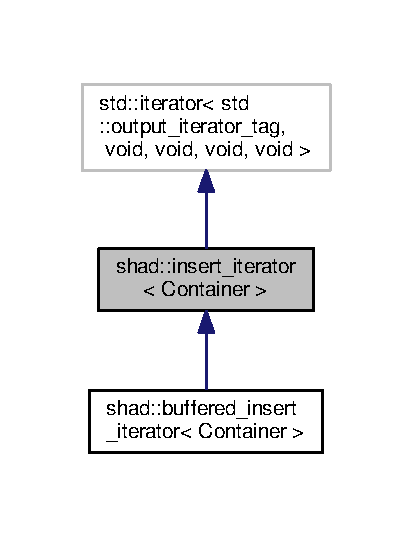
\includegraphics[width=198pt]{classshad_1_1insert__iterator__inherit__graph}
\end{center}
\end{figure}


Collaboration diagram for shad\-:\-:insert\-\_\-iterator$<$ Container $>$\-:
\nopagebreak
\begin{figure}[H]
\begin{center}
\leavevmode
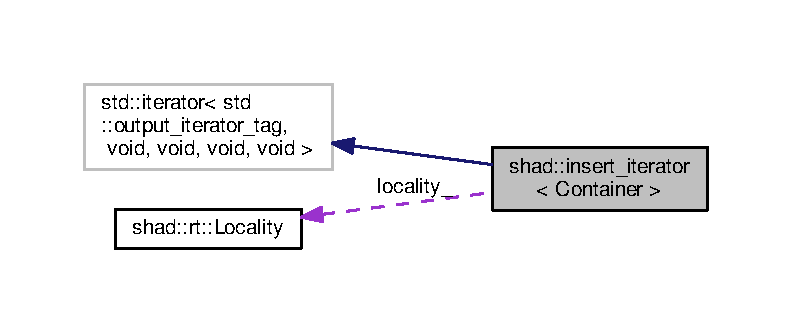
\includegraphics[width=350pt]{classshad_1_1insert__iterator__coll__graph}
\end{center}
\end{figure}
\subsection*{Public Types}
\begin{DoxyCompactItemize}
\item 
using \hyperlink{classshad_1_1insert__iterator_a0a364f131900a4898acb9a8e499c6070}{value\-\_\-type} = typename Container\-::value\-\_\-type
\item 
using \hyperlink{classshad_1_1insert__iterator_a0ab6d747c808ebbaf2e00213490585f4}{container\-\_\-type} = Container
\end{DoxyCompactItemize}
\subsection*{Public Member Functions}
\begin{DoxyCompactItemize}
\item 
\hyperlink{classshad_1_1insert__iterator_a2285f56ef6b37912b8af1700f39e62f1}{insert\-\_\-iterator} (Container \&container, \hyperlink{classshad_1_1insert__iterator_a9423151fee020bc148d8c6037ecb0542}{Iterator} iterator)
\begin{DoxyCompactList}\small\item\em Constructor. \end{DoxyCompactList}\item 
\hyperlink{classshad_1_1insert__iterator}{insert\-\_\-iterator} \& \hyperlink{classshad_1_1insert__iterator_a8f5d1c522b2f339db25b69974a41e0d6}{operator=} (const \hyperlink{classshad_1_1insert__iterator_a0a364f131900a4898acb9a8e499c6070}{value\-\_\-type} \&value)
\begin{DoxyCompactList}\small\item\em The assignment operator. \end{DoxyCompactList}\item 
\hyperlink{classshad_1_1insert__iterator}{insert\-\_\-iterator} \& \hyperlink{classshad_1_1insert__iterator_a58059a463666bc70b7804c399317d87d}{operator$\ast$} ()
\item 
\hyperlink{classshad_1_1insert__iterator}{insert\-\_\-iterator} \& \hyperlink{classshad_1_1insert__iterator_adf7bda892033b37e6cb139b62350c9c2}{operator++} ()
\item 
\hyperlink{classshad_1_1insert__iterator}{insert\-\_\-iterator} \& \hyperlink{classshad_1_1insert__iterator_ad5ce27986d772edaabee569317b49ec5}{operator++} (int)
\end{DoxyCompactItemize}
\subsection*{Protected Types}
\begin{DoxyCompactItemize}
\item 
using \hyperlink{classshad_1_1insert__iterator_a9423151fee020bc148d8c6037ecb0542}{Iterator} = typename Container\-::iterator
\item 
using \hyperlink{classshad_1_1insert__iterator_a040650a6a725c67ff6b4331cef06afaa}{internal\-\_\-container\-\_\-t} = typename Container\-::internal\-\_\-container\-\_\-t
\end{DoxyCompactItemize}
\subsection*{Protected Attributes}
\begin{DoxyCompactItemize}
\item 
internal\-\_\-container\-\_\-t\-::\-Object\-I\-D \hyperlink{classshad_1_1insert__iterator_ab90ac3bffe8239a3d5472ad669164597}{global\-\_\-id\-\_\-}
\item 
\hyperlink{classshad_1_1insert__iterator_a9423151fee020bc148d8c6037ecb0542}{Iterator} \hyperlink{classshad_1_1insert__iterator_a0d26bcdf8d5485fd5a703245bb9d75a5}{iterator\-\_\-}
\item 
\hyperlink{classshad_1_1insert__iterator_a040650a6a725c67ff6b4331cef06afaa}{internal\-\_\-container\-\_\-t} $\ast$ \hyperlink{classshad_1_1insert__iterator_ab1fb4edf1ef845937bf22731526c2b9e}{local\-\_\-container\-\_\-ptr\-\_\-} = nullptr
\item 
\hyperlink{classshad_1_1rt_1_1Locality}{rt\-::\-Locality} \hyperlink{classshad_1_1insert__iterator_a5b9dc5f15bd6d1aa377a9befe7f14ae5}{locality\-\_\-}
\end{DoxyCompactItemize}


\subsection{Detailed Description}
\subsubsection*{template$<$typename Container$>$class shad\-::insert\-\_\-iterator$<$ Container $>$}

Insert iterator (over a shad container). 

\hyperlink{classshad_1_1insert__iterator}{shad\-::insert\-\_\-iterator} is an Output\-Iterator that inserts elements into a distributed container for which it was constructed, at the position pointed to by the supplied iterator. The buffered insertion is performed whenever the iterator (whether dereferenced or not) is assigned to. Incrementing the \hyperlink{classshad_1_1buffered__insert__iterator}{shad\-::buffered\-\_\-insert\-\_\-iterator} is a no-\/op.


\begin{DoxyTemplParams}{Template Parameters}
{\em Container} & The type of the distributed container. \\
\hline
\end{DoxyTemplParams}


\subsection{Member Typedef Documentation}
\hypertarget{classshad_1_1insert__iterator_a0ab6d747c808ebbaf2e00213490585f4}{\index{shad\-::insert\-\_\-iterator@{shad\-::insert\-\_\-iterator}!container\-\_\-type@{container\-\_\-type}}
\index{container\-\_\-type@{container\-\_\-type}!shad::insert_iterator@{shad\-::insert\-\_\-iterator}}
\subsubsection[{container\-\_\-type}]{\setlength{\rightskip}{0pt plus 5cm}template$<$typename Container $>$ using {\bf shad\-::insert\-\_\-iterator}$<$ Container $>$\-::{\bf container\-\_\-type} =  Container}}\label{classshad_1_1insert__iterator_a0ab6d747c808ebbaf2e00213490585f4}
\hypertarget{classshad_1_1insert__iterator_a040650a6a725c67ff6b4331cef06afaa}{\index{shad\-::insert\-\_\-iterator@{shad\-::insert\-\_\-iterator}!internal\-\_\-container\-\_\-t@{internal\-\_\-container\-\_\-t}}
\index{internal\-\_\-container\-\_\-t@{internal\-\_\-container\-\_\-t}!shad::insert_iterator@{shad\-::insert\-\_\-iterator}}
\subsubsection[{internal\-\_\-container\-\_\-t}]{\setlength{\rightskip}{0pt plus 5cm}template$<$typename Container $>$ using {\bf shad\-::insert\-\_\-iterator}$<$ Container $>$\-::{\bf internal\-\_\-container\-\_\-t} =  typename Container\-::internal\-\_\-container\-\_\-t\hspace{0.3cm}{\ttfamily [protected]}}}\label{classshad_1_1insert__iterator_a040650a6a725c67ff6b4331cef06afaa}
\hypertarget{classshad_1_1insert__iterator_a9423151fee020bc148d8c6037ecb0542}{\index{shad\-::insert\-\_\-iterator@{shad\-::insert\-\_\-iterator}!Iterator@{Iterator}}
\index{Iterator@{Iterator}!shad::insert_iterator@{shad\-::insert\-\_\-iterator}}
\subsubsection[{Iterator}]{\setlength{\rightskip}{0pt plus 5cm}template$<$typename Container $>$ using {\bf shad\-::insert\-\_\-iterator}$<$ Container $>$\-::{\bf Iterator} =  typename Container\-::iterator\hspace{0.3cm}{\ttfamily [protected]}}}\label{classshad_1_1insert__iterator_a9423151fee020bc148d8c6037ecb0542}
\hypertarget{classshad_1_1insert__iterator_a0a364f131900a4898acb9a8e499c6070}{\index{shad\-::insert\-\_\-iterator@{shad\-::insert\-\_\-iterator}!value\-\_\-type@{value\-\_\-type}}
\index{value\-\_\-type@{value\-\_\-type}!shad::insert_iterator@{shad\-::insert\-\_\-iterator}}
\subsubsection[{value\-\_\-type}]{\setlength{\rightskip}{0pt plus 5cm}template$<$typename Container $>$ using {\bf shad\-::insert\-\_\-iterator}$<$ Container $>$\-::{\bf value\-\_\-type} =  typename Container\-::value\-\_\-type}}\label{classshad_1_1insert__iterator_a0a364f131900a4898acb9a8e499c6070}


\subsection{Constructor \& Destructor Documentation}
\hypertarget{classshad_1_1insert__iterator_a2285f56ef6b37912b8af1700f39e62f1}{\index{shad\-::insert\-\_\-iterator@{shad\-::insert\-\_\-iterator}!insert\-\_\-iterator@{insert\-\_\-iterator}}
\index{insert\-\_\-iterator@{insert\-\_\-iterator}!shad::insert_iterator@{shad\-::insert\-\_\-iterator}}
\subsubsection[{insert\-\_\-iterator}]{\setlength{\rightskip}{0pt plus 5cm}template$<$typename Container $>$ {\bf shad\-::insert\-\_\-iterator}$<$ Container $>$\-::{\bf insert\-\_\-iterator} (
\begin{DoxyParamCaption}
\item[{Container \&}]{container, }
\item[{{\bf Iterator}}]{iterator}
\end{DoxyParamCaption}
)\hspace{0.3cm}{\ttfamily [inline]}}}\label{classshad_1_1insert__iterator_a2285f56ef6b37912b8af1700f39e62f1}


Constructor. 


\begin{DoxyParams}{Parameters}
{\em container} & The container into which the iterator inserts. \\
\hline
{\em iterator} & The position at which the iterator starts to insert. \\
\hline
\end{DoxyParams}


\subsection{Member Function Documentation}
\hypertarget{classshad_1_1insert__iterator_a58059a463666bc70b7804c399317d87d}{\index{shad\-::insert\-\_\-iterator@{shad\-::insert\-\_\-iterator}!operator$\ast$@{operator$\ast$}}
\index{operator$\ast$@{operator$\ast$}!shad::insert_iterator@{shad\-::insert\-\_\-iterator}}
\subsubsection[{operator$\ast$}]{\setlength{\rightskip}{0pt plus 5cm}template$<$typename Container $>$ {\bf insert\-\_\-iterator}\& {\bf shad\-::insert\-\_\-iterator}$<$ Container $>$\-::operator$\ast$ (
\begin{DoxyParamCaption}
{}
\end{DoxyParamCaption}
)\hspace{0.3cm}{\ttfamily [inline]}}}\label{classshad_1_1insert__iterator_a58059a463666bc70b7804c399317d87d}
\hypertarget{classshad_1_1insert__iterator_adf7bda892033b37e6cb139b62350c9c2}{\index{shad\-::insert\-\_\-iterator@{shad\-::insert\-\_\-iterator}!operator++@{operator++}}
\index{operator++@{operator++}!shad::insert_iterator@{shad\-::insert\-\_\-iterator}}
\subsubsection[{operator++}]{\setlength{\rightskip}{0pt plus 5cm}template$<$typename Container $>$ {\bf insert\-\_\-iterator}\& {\bf shad\-::insert\-\_\-iterator}$<$ Container $>$\-::operator++ (
\begin{DoxyParamCaption}
{}
\end{DoxyParamCaption}
)\hspace{0.3cm}{\ttfamily [inline]}}}\label{classshad_1_1insert__iterator_adf7bda892033b37e6cb139b62350c9c2}
\hypertarget{classshad_1_1insert__iterator_ad5ce27986d772edaabee569317b49ec5}{\index{shad\-::insert\-\_\-iterator@{shad\-::insert\-\_\-iterator}!operator++@{operator++}}
\index{operator++@{operator++}!shad::insert_iterator@{shad\-::insert\-\_\-iterator}}
\subsubsection[{operator++}]{\setlength{\rightskip}{0pt plus 5cm}template$<$typename Container $>$ {\bf insert\-\_\-iterator}\& {\bf shad\-::insert\-\_\-iterator}$<$ Container $>$\-::operator++ (
\begin{DoxyParamCaption}
\item[{int}]{}
\end{DoxyParamCaption}
)\hspace{0.3cm}{\ttfamily [inline]}}}\label{classshad_1_1insert__iterator_ad5ce27986d772edaabee569317b49ec5}
\hypertarget{classshad_1_1insert__iterator_a8f5d1c522b2f339db25b69974a41e0d6}{\index{shad\-::insert\-\_\-iterator@{shad\-::insert\-\_\-iterator}!operator=@{operator=}}
\index{operator=@{operator=}!shad::insert_iterator@{shad\-::insert\-\_\-iterator}}
\subsubsection[{operator=}]{\setlength{\rightskip}{0pt plus 5cm}template$<$typename Container $>$ {\bf insert\-\_\-iterator}\& {\bf shad\-::insert\-\_\-iterator}$<$ Container $>$\-::operator= (
\begin{DoxyParamCaption}
\item[{const {\bf value\-\_\-type} \&}]{value}
\end{DoxyParamCaption}
)\hspace{0.3cm}{\ttfamily [inline]}}}\label{classshad_1_1insert__iterator_a8f5d1c522b2f339db25b69974a41e0d6}


The assignment operator. 

The assignment operator inserts a value (through buffering) and advance iterator.


\begin{DoxyParams}{Parameters}
{\em value} & A const reference to the value to be inserted.\\
\hline
\end{DoxyParams}
\begin{DoxyReturn}{Returns}
A self reference. 
\end{DoxyReturn}


\subsection{Member Data Documentation}
\hypertarget{classshad_1_1insert__iterator_ab90ac3bffe8239a3d5472ad669164597}{\index{shad\-::insert\-\_\-iterator@{shad\-::insert\-\_\-iterator}!global\-\_\-id\-\_\-@{global\-\_\-id\-\_\-}}
\index{global\-\_\-id\-\_\-@{global\-\_\-id\-\_\-}!shad::insert_iterator@{shad\-::insert\-\_\-iterator}}
\subsubsection[{global\-\_\-id\-\_\-}]{\setlength{\rightskip}{0pt plus 5cm}template$<$typename Container $>$ internal\-\_\-container\-\_\-t\-::\-Object\-I\-D {\bf shad\-::insert\-\_\-iterator}$<$ Container $>$\-::global\-\_\-id\-\_\-\hspace{0.3cm}{\ttfamily [protected]}}}\label{classshad_1_1insert__iterator_ab90ac3bffe8239a3d5472ad669164597}
\hypertarget{classshad_1_1insert__iterator_a0d26bcdf8d5485fd5a703245bb9d75a5}{\index{shad\-::insert\-\_\-iterator@{shad\-::insert\-\_\-iterator}!iterator\-\_\-@{iterator\-\_\-}}
\index{iterator\-\_\-@{iterator\-\_\-}!shad::insert_iterator@{shad\-::insert\-\_\-iterator}}
\subsubsection[{iterator\-\_\-}]{\setlength{\rightskip}{0pt plus 5cm}template$<$typename Container $>$ {\bf Iterator} {\bf shad\-::insert\-\_\-iterator}$<$ Container $>$\-::iterator\-\_\-\hspace{0.3cm}{\ttfamily [protected]}}}\label{classshad_1_1insert__iterator_a0d26bcdf8d5485fd5a703245bb9d75a5}
\hypertarget{classshad_1_1insert__iterator_ab1fb4edf1ef845937bf22731526c2b9e}{\index{shad\-::insert\-\_\-iterator@{shad\-::insert\-\_\-iterator}!local\-\_\-container\-\_\-ptr\-\_\-@{local\-\_\-container\-\_\-ptr\-\_\-}}
\index{local\-\_\-container\-\_\-ptr\-\_\-@{local\-\_\-container\-\_\-ptr\-\_\-}!shad::insert_iterator@{shad\-::insert\-\_\-iterator}}
\subsubsection[{local\-\_\-container\-\_\-ptr\-\_\-}]{\setlength{\rightskip}{0pt plus 5cm}template$<$typename Container $>$ {\bf internal\-\_\-container\-\_\-t}$\ast$ {\bf shad\-::insert\-\_\-iterator}$<$ Container $>$\-::local\-\_\-container\-\_\-ptr\-\_\- = nullptr\hspace{0.3cm}{\ttfamily [protected]}}}\label{classshad_1_1insert__iterator_ab1fb4edf1ef845937bf22731526c2b9e}
\hypertarget{classshad_1_1insert__iterator_a5b9dc5f15bd6d1aa377a9befe7f14ae5}{\index{shad\-::insert\-\_\-iterator@{shad\-::insert\-\_\-iterator}!locality\-\_\-@{locality\-\_\-}}
\index{locality\-\_\-@{locality\-\_\-}!shad::insert_iterator@{shad\-::insert\-\_\-iterator}}
\subsubsection[{locality\-\_\-}]{\setlength{\rightskip}{0pt plus 5cm}template$<$typename Container $>$ {\bf rt\-::\-Locality} {\bf shad\-::insert\-\_\-iterator}$<$ Container $>$\-::locality\-\_\-\hspace{0.3cm}{\ttfamily [protected]}}}\label{classshad_1_1insert__iterator_a5b9dc5f15bd6d1aa377a9befe7f14ae5}


The documentation for this class was generated from the following file\-:\begin{DoxyCompactItemize}
\item 
include/shad/core/\hyperlink{iterator_8h}{iterator.\-h}\end{DoxyCompactItemize}

\hypertarget{structshad_1_1is__block__contiguous}{\section{shad\-:\-:is\-\_\-block\-\_\-contiguous$<$ It $>$ Struct Template Reference}
\label{structshad_1_1is__block__contiguous}\index{shad\-::is\-\_\-block\-\_\-contiguous$<$ It $>$@{shad\-::is\-\_\-block\-\_\-contiguous$<$ It $>$}}
}


{\ttfamily \#include $<$shad/core/iterator.\-h$>$}

\subsection*{Static Public Attributes}
\begin{DoxyCompactItemize}
\item 
static constexpr std\-::true\-\_\-type \hyperlink{structshad_1_1is__block__contiguous_a3a6d6b8fadc20fcf7d737de0b9a1f567}{value} \{\}
\end{DoxyCompactItemize}


\subsection{Member Data Documentation}
\hypertarget{structshad_1_1is__block__contiguous_a3a6d6b8fadc20fcf7d737de0b9a1f567}{\index{shad\-::is\-\_\-block\-\_\-contiguous@{shad\-::is\-\_\-block\-\_\-contiguous}!value@{value}}
\index{value@{value}!shad::is_block_contiguous@{shad\-::is\-\_\-block\-\_\-contiguous}}
\subsubsection[{value}]{\setlength{\rightskip}{0pt plus 5cm}template$<$typename It $>$ constexpr std\-::true\-\_\-type {\bf shad\-::is\-\_\-block\-\_\-contiguous}$<$ It $>$\-::value \{\}\hspace{0.3cm}{\ttfamily [static]}}}\label{structshad_1_1is__block__contiguous_a3a6d6b8fadc20fcf7d737de0b9a1f567}


The documentation for this struct was generated from the following file\-:\begin{DoxyCompactItemize}
\item 
include/shad/core/\hyperlink{iterator_8h}{iterator.\-h}\end{DoxyCompactItemize}

\hypertarget{structshad_1_1is__block__contiguous_3_01shad_1_1buffered__insert__iterator_3_01Container_01_4_01_4}{\section{shad\-:\-:is\-\_\-block\-\_\-contiguous$<$ shad\-:\-:buffered\-\_\-insert\-\_\-iterator$<$ Container $>$ $>$ Struct Template Reference}
\label{structshad_1_1is__block__contiguous_3_01shad_1_1buffered__insert__iterator_3_01Container_01_4_01_4}\index{shad\-::is\-\_\-block\-\_\-contiguous$<$ shad\-::buffered\-\_\-insert\-\_\-iterator$<$ Container $>$ $>$@{shad\-::is\-\_\-block\-\_\-contiguous$<$ shad\-::buffered\-\_\-insert\-\_\-iterator$<$ Container $>$ $>$}}
}


{\ttfamily \#include $<$shad/core/iterator.\-h$>$}

\subsection*{Static Public Attributes}
\begin{DoxyCompactItemize}
\item 
static constexpr std\-::false\-\_\-type \hyperlink{structshad_1_1is__block__contiguous_3_01shad_1_1buffered__insert__iterator_3_01Container_01_4_01_4_ae664f81d1ba1a6f009d700cbfb337f65}{value} \{\}
\end{DoxyCompactItemize}


\subsection{Member Data Documentation}
\hypertarget{structshad_1_1is__block__contiguous_3_01shad_1_1buffered__insert__iterator_3_01Container_01_4_01_4_ae664f81d1ba1a6f009d700cbfb337f65}{\index{shad\-::is\-\_\-block\-\_\-contiguous$<$ shad\-::buffered\-\_\-insert\-\_\-iterator$<$ Container $>$ $>$@{shad\-::is\-\_\-block\-\_\-contiguous$<$ shad\-::buffered\-\_\-insert\-\_\-iterator$<$ Container $>$ $>$}!value@{value}}
\index{value@{value}!shad::is_block_contiguous< shad::buffered_insert_iterator< Container > >@{shad\-::is\-\_\-block\-\_\-contiguous$<$ shad\-::buffered\-\_\-insert\-\_\-iterator$<$ Container $>$ $>$}}
\subsubsection[{value}]{\setlength{\rightskip}{0pt plus 5cm}template$<$typename Container $>$ constexpr std\-::false\-\_\-type {\bf shad\-::is\-\_\-block\-\_\-contiguous}$<$ {\bf shad\-::buffered\-\_\-insert\-\_\-iterator}$<$ Container $>$ $>$\-::value \{\}\hspace{0.3cm}{\ttfamily [static]}}}\label{structshad_1_1is__block__contiguous_3_01shad_1_1buffered__insert__iterator_3_01Container_01_4_01_4_ae664f81d1ba1a6f009d700cbfb337f65}


The documentation for this struct was generated from the following file\-:\begin{DoxyCompactItemize}
\item 
include/shad/core/\hyperlink{iterator_8h}{iterator.\-h}\end{DoxyCompactItemize}

\hypertarget{structshad_1_1is__block__contiguous_3_01shad_1_1insert__iterator_3_01Container_01_4_01_4}{\section{shad\-:\-:is\-\_\-block\-\_\-contiguous$<$ shad\-:\-:insert\-\_\-iterator$<$ Container $>$ $>$ Struct Template Reference}
\label{structshad_1_1is__block__contiguous_3_01shad_1_1insert__iterator_3_01Container_01_4_01_4}\index{shad\-::is\-\_\-block\-\_\-contiguous$<$ shad\-::insert\-\_\-iterator$<$ Container $>$ $>$@{shad\-::is\-\_\-block\-\_\-contiguous$<$ shad\-::insert\-\_\-iterator$<$ Container $>$ $>$}}
}


{\ttfamily \#include $<$shad/core/iterator.\-h$>$}

\subsection*{Static Public Attributes}
\begin{DoxyCompactItemize}
\item 
static constexpr std\-::false\-\_\-type \hyperlink{structshad_1_1is__block__contiguous_3_01shad_1_1insert__iterator_3_01Container_01_4_01_4_ac1de637c6b8719fbfa91ae95d5c9dadd}{value} \{\}
\end{DoxyCompactItemize}


\subsection{Member Data Documentation}
\hypertarget{structshad_1_1is__block__contiguous_3_01shad_1_1insert__iterator_3_01Container_01_4_01_4_ac1de637c6b8719fbfa91ae95d5c9dadd}{\index{shad\-::is\-\_\-block\-\_\-contiguous$<$ shad\-::insert\-\_\-iterator$<$ Container $>$ $>$@{shad\-::is\-\_\-block\-\_\-contiguous$<$ shad\-::insert\-\_\-iterator$<$ Container $>$ $>$}!value@{value}}
\index{value@{value}!shad::is_block_contiguous< shad::insert_iterator< Container > >@{shad\-::is\-\_\-block\-\_\-contiguous$<$ shad\-::insert\-\_\-iterator$<$ Container $>$ $>$}}
\subsubsection[{value}]{\setlength{\rightskip}{0pt plus 5cm}template$<$typename Container $>$ constexpr std\-::false\-\_\-type {\bf shad\-::is\-\_\-block\-\_\-contiguous}$<$ {\bf shad\-::insert\-\_\-iterator}$<$ Container $>$ $>$\-::value \{\}\hspace{0.3cm}{\ttfamily [static]}}}\label{structshad_1_1is__block__contiguous_3_01shad_1_1insert__iterator_3_01Container_01_4_01_4_ac1de637c6b8719fbfa91ae95d5c9dadd}


The documentation for this struct was generated from the following file\-:\begin{DoxyCompactItemize}
\item 
include/shad/core/\hyperlink{iterator_8h}{iterator.\-h}\end{DoxyCompactItemize}

\hypertarget{structshad_1_1is__distributed__iterator}{\section{shad\-:\-:is\-\_\-distributed\-\_\-iterator$<$ T, typename $>$ Struct Template Reference}
\label{structshad_1_1is__distributed__iterator}\index{shad\-::is\-\_\-distributed\-\_\-iterator$<$ T, typename $>$@{shad\-::is\-\_\-distributed\-\_\-iterator$<$ T, typename $>$}}
}


{\ttfamily \#include $<$shad/distributed\-\_\-iterator\-\_\-traits.\-h$>$}

\subsection*{Static Public Attributes}
\begin{DoxyCompactItemize}
\item 
static constexpr bool \hyperlink{structshad_1_1is__distributed__iterator_a8eff7da7d0308d61ac32d008fe4a4219}{value} = false
\end{DoxyCompactItemize}


\subsection{Member Data Documentation}
\hypertarget{structshad_1_1is__distributed__iterator_a8eff7da7d0308d61ac32d008fe4a4219}{\index{shad\-::is\-\_\-distributed\-\_\-iterator@{shad\-::is\-\_\-distributed\-\_\-iterator}!value@{value}}
\index{value@{value}!shad::is_distributed_iterator@{shad\-::is\-\_\-distributed\-\_\-iterator}}
\subsubsection[{value}]{\setlength{\rightskip}{0pt plus 5cm}template$<$typename T , typename  = void$>$ constexpr bool {\bf shad\-::is\-\_\-distributed\-\_\-iterator}$<$ T, typename $>$\-::value = false\hspace{0.3cm}{\ttfamily [static]}}}\label{structshad_1_1is__distributed__iterator_a8eff7da7d0308d61ac32d008fe4a4219}


The documentation for this struct was generated from the following file\-:\begin{DoxyCompactItemize}
\item 
include/shad/\hyperlink{distributed__iterator__traits_8h}{distributed\-\_\-iterator\-\_\-traits.\-h}\end{DoxyCompactItemize}

\hypertarget{structshad_1_1is__distributed__iterator_3_01T_00_01typename_01std_1_1enable__if_3_9std_1_1is__sa51db7b1d56bd82f65c31391ac3bbe077}{\section{shad\-:\-:is\-\_\-distributed\-\_\-iterator$<$ T, typename std\-:\-:enable\-\_\-if$<$!std\-:\-:is\-\_\-same$<$ typename distributed\-\_\-iterator\-\_\-traits$<$ T $>$\-:\-:value\-\_\-type, void $>$\-:\-:value $>$\-:\-:type $>$ Struct Template Reference}
\label{structshad_1_1is__distributed__iterator_3_01T_00_01typename_01std_1_1enable__if_3_9std_1_1is__sa51db7b1d56bd82f65c31391ac3bbe077}\index{shad\-::is\-\_\-distributed\-\_\-iterator$<$ T, typename std\-::enable\-\_\-if$<$!std\-::is\-\_\-same$<$ typename distributed\-\_\-iterator\-\_\-traits$<$ T $>$\-::value\-\_\-type, void $>$\-::value $>$\-::type $>$@{shad\-::is\-\_\-distributed\-\_\-iterator$<$ T, typename std\-::enable\-\_\-if$<$!std\-::is\-\_\-same$<$ typename distributed\-\_\-iterator\-\_\-traits$<$ T $>$\-::value\-\_\-type, void $>$\-::value $>$\-::type $>$}}
}


{\ttfamily \#include $<$shad/distributed\-\_\-iterator\-\_\-traits.\-h$>$}

\subsection*{Static Public Attributes}
\begin{DoxyCompactItemize}
\item 
static constexpr bool \hyperlink{structshad_1_1is__distributed__iterator_3_01T_00_01typename_01std_1_1enable__if_3_9std_1_1is__sa51db7b1d56bd82f65c31391ac3bbe077_a1cfb04895451ff68d946df3e4b15ba7d}{value} = true
\end{DoxyCompactItemize}


\subsection{Member Data Documentation}
\hypertarget{structshad_1_1is__distributed__iterator_3_01T_00_01typename_01std_1_1enable__if_3_9std_1_1is__sa51db7b1d56bd82f65c31391ac3bbe077_a1cfb04895451ff68d946df3e4b15ba7d}{\index{shad\-::is\-\_\-distributed\-\_\-iterator$<$ T, typename std\-::enable\-\_\-if$<$!std\-::is\-\_\-same$<$ typename distributed\-\_\-iterator\-\_\-traits$<$ T $>$\-::value\-\_\-type, void $>$\-::value $>$\-::type $>$@{shad\-::is\-\_\-distributed\-\_\-iterator$<$ T, typename std\-::enable\-\_\-if$<$!std\-::is\-\_\-same$<$ typename distributed\-\_\-iterator\-\_\-traits$<$ T $>$\-::value\-\_\-type, void $>$\-::value $>$\-::type $>$}!value@{value}}
\index{value@{value}!shad::is_distributed_iterator< T, typename std::enable_if<!std::is_same< typename distributed_iterator_traits< T >::value_type, void >::value >::type >@{shad\-::is\-\_\-distributed\-\_\-iterator$<$ T, typename std\-::enable\-\_\-if$<$!std\-::is\-\_\-same$<$ typename distributed\-\_\-iterator\-\_\-traits$<$ T $>$\-::value\-\_\-type, void $>$\-::value $>$\-::type $>$}}
\subsubsection[{value}]{\setlength{\rightskip}{0pt plus 5cm}template$<$typename T $>$ constexpr bool {\bf shad\-::is\-\_\-distributed\-\_\-iterator}$<$ T, typename std\-::enable\-\_\-if$<$!std\-::is\-\_\-same$<$ typename {\bf distributed\-\_\-iterator\-\_\-traits}$<$ T $>$\-::value\-\_\-type, void $>$\-::value $>$\-::type $>$\-::value = true\hspace{0.3cm}{\ttfamily [static]}}}\label{structshad_1_1is__distributed__iterator_3_01T_00_01typename_01std_1_1enable__if_3_9std_1_1is__sa51db7b1d56bd82f65c31391ac3bbe077_a1cfb04895451ff68d946df3e4b15ba7d}


The documentation for this struct was generated from the following file\-:\begin{DoxyCompactItemize}
\item 
include/shad/\hyperlink{distributed__iterator__traits_8h}{distributed\-\_\-iterator\-\_\-traits.\-h}\end{DoxyCompactItemize}

\hypertarget{structshad_1_1is__execution__policy}{\section{shad\-:\-:is\-\_\-execution\-\_\-policy$<$ Execution\-Policy $>$ Struct Template Reference}
\label{structshad_1_1is__execution__policy}\index{shad\-::is\-\_\-execution\-\_\-policy$<$ Execution\-Policy $>$@{shad\-::is\-\_\-execution\-\_\-policy$<$ Execution\-Policy $>$}}
}


{\ttfamily \#include $<$shad/core/execution.\-h$>$}



Inheritance diagram for shad\-:\-:is\-\_\-execution\-\_\-policy$<$ Execution\-Policy $>$\-:
\nopagebreak
\begin{figure}[H]
\begin{center}
\leavevmode
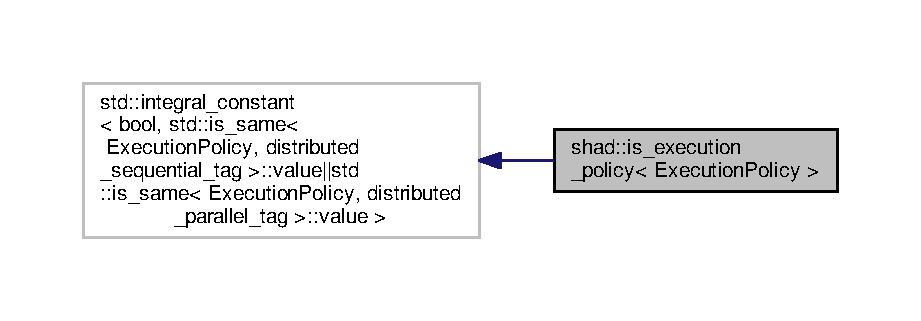
\includegraphics[width=350pt]{structshad_1_1is__execution__policy__inherit__graph}
\end{center}
\end{figure}


Collaboration diagram for shad\-:\-:is\-\_\-execution\-\_\-policy$<$ Execution\-Policy $>$\-:
\nopagebreak
\begin{figure}[H]
\begin{center}
\leavevmode
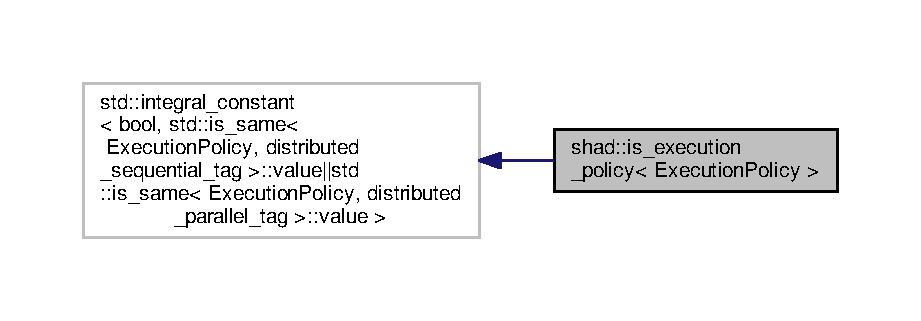
\includegraphics[width=350pt]{structshad_1_1is__execution__policy__coll__graph}
\end{center}
\end{figure}


The documentation for this struct was generated from the following file\-:\begin{DoxyCompactItemize}
\item 
include/shad/core/\hyperlink{execution_8h}{execution.\-h}\end{DoxyCompactItemize}

\hypertarget{structshad_1_1is__std__hashable}{\section{shad\-:\-:is\-\_\-std\-\_\-hashable$<$ T $>$ Struct Template Reference}
\label{structshad_1_1is__std__hashable}\index{shad\-::is\-\_\-std\-\_\-hashable$<$ T $>$@{shad\-::is\-\_\-std\-\_\-hashable$<$ T $>$}}
}


{\ttfamily \#include $<$shad/core/type\-\_\-traits.\-h$>$}



Inheritance diagram for shad\-:\-:is\-\_\-std\-\_\-hashable$<$ T $>$\-:
\nopagebreak
\begin{figure}[H]
\begin{center}
\leavevmode
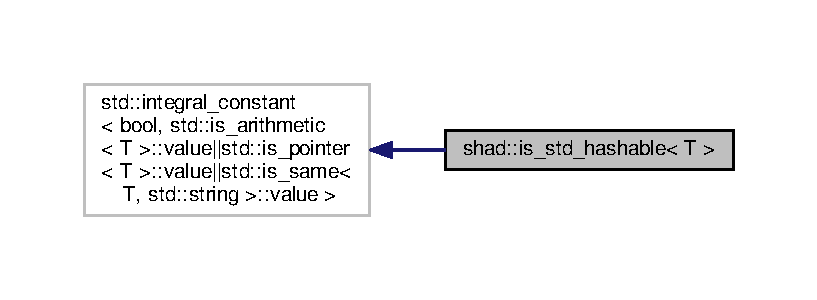
\includegraphics[width=350pt]{structshad_1_1is__std__hashable__inherit__graph}
\end{center}
\end{figure}


Collaboration diagram for shad\-:\-:is\-\_\-std\-\_\-hashable$<$ T $>$\-:
\nopagebreak
\begin{figure}[H]
\begin{center}
\leavevmode
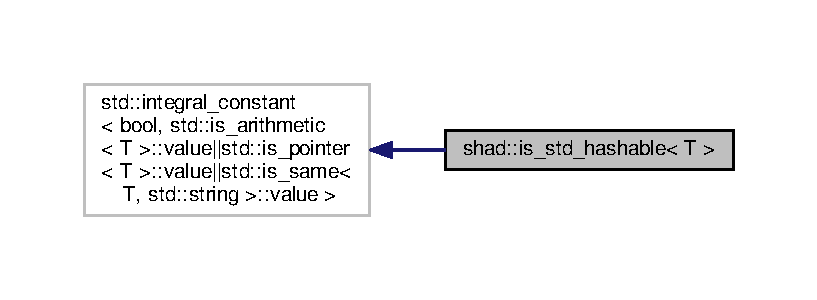
\includegraphics[width=350pt]{structshad_1_1is__std__hashable__coll__graph}
\end{center}
\end{figure}


The documentation for this struct was generated from the following file\-:\begin{DoxyCompactItemize}
\item 
include/shad/core/\hyperlink{type__traits_8h}{type\-\_\-traits.\-h}\end{DoxyCompactItemize}

\hypertarget{classshad_1_1lmap__iterator}{\section{shad\-:\-:lmap\-\_\-iterator$<$ L\-Map, T $>$ Class Template Reference}
\label{classshad_1_1lmap__iterator}\index{shad\-::lmap\-\_\-iterator$<$ L\-Map, T $>$@{shad\-::lmap\-\_\-iterator$<$ L\-Map, T $>$}}
}


{\ttfamily \#include $<$shad/data\-\_\-structures/local\-\_\-hashmap.\-h$>$}



Inheritance diagram for shad\-:\-:lmap\-\_\-iterator$<$ L\-Map, T $>$\-:
\nopagebreak
\begin{figure}[H]
\begin{center}
\leavevmode
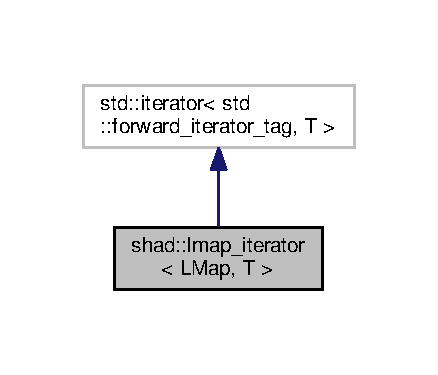
\includegraphics[width=210pt]{classshad_1_1lmap__iterator__inherit__graph}
\end{center}
\end{figure}


Collaboration diagram for shad\-:\-:lmap\-\_\-iterator$<$ L\-Map, T $>$\-:
\nopagebreak
\begin{figure}[H]
\begin{center}
\leavevmode
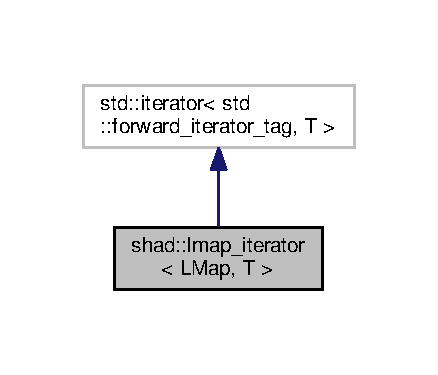
\includegraphics[width=210pt]{classshad_1_1lmap__iterator__coll__graph}
\end{center}
\end{figure}
\subsection*{Public Types}
\begin{DoxyCompactItemize}
\item 
using \hyperlink{classshad_1_1lmap__iterator_a5aaca46b07b8669790d0134b6f4a9f97}{value\-\_\-type} = T
\item 
using \hyperlink{classshad_1_1lmap__iterator_a67f31795cef049e504582e3ec92232ba}{Entry} = typename L\-Map\-::\-Entry
\item 
using \hyperlink{classshad_1_1lmap__iterator_a21e8efc8bee9e50f89cd3c17a0c18673}{State} = typename L\-Map\-::\-State
\item 
using \hyperlink{classshad_1_1lmap__iterator_aa37c8a6e06e10d9256e3ce2be6fabb4a}{Bucket} = typename L\-Map\-::\-Bucket
\end{DoxyCompactItemize}
\subsection*{Public Member Functions}
\begin{DoxyCompactItemize}
\item 
\hyperlink{classshad_1_1lmap__iterator_a56f6c9d476d6ad8d8693554c80c32bca}{lmap\-\_\-iterator} ()
\item 
\hyperlink{classshad_1_1lmap__iterator_a692400133c2520870cec48845f46aa5b}{lmap\-\_\-iterator} (const L\-Map $\ast$map\-Ptr, size\-\_\-t b\-Id, size\-\_\-t pos, \hyperlink{classshad_1_1lmap__iterator_aa37c8a6e06e10d9256e3ce2be6fabb4a}{Bucket} $\ast$cb, \hyperlink{classshad_1_1lmap__iterator_a67f31795cef049e504582e3ec92232ba}{Entry} $\ast$e\-Ptr)
\item 
bool \hyperlink{classshad_1_1lmap__iterator_ad07acefab2006a2836fef3e333eb615c}{operator==} (const \hyperlink{classshad_1_1lmap__iterator}{lmap\-\_\-iterator} \&other) const 
\item 
bool \hyperlink{classshad_1_1lmap__iterator_a9805a06dcd00b59d7e66184ab1deabd1}{operator!=} (const \hyperlink{classshad_1_1lmap__iterator}{lmap\-\_\-iterator} \&other) const 
\item 
T \hyperlink{classshad_1_1lmap__iterator_a0a93b6df2a3dd0a342f018bae3700d95}{operator$\ast$} () const 
\item 
\hyperlink{classshad_1_1lmap__iterator}{lmap\-\_\-iterator} \& \hyperlink{classshad_1_1lmap__iterator_a2fb20e73193dc51da1278f91724a119e}{operator++} ()
\item 
\hyperlink{classshad_1_1lmap__iterator}{lmap\-\_\-iterator} \hyperlink{classshad_1_1lmap__iterator_abba47ae81bde6f3ad2ff31327aa6f68c}{operator++} (int)
\end{DoxyCompactItemize}
\subsection*{Static Public Member Functions}
\begin{DoxyCompactItemize}
\item 
static \hyperlink{classshad_1_1lmap__iterator}{lmap\-\_\-iterator} \hyperlink{classshad_1_1lmap__iterator_a77957036c48c709283ed2ec98fe79e0d}{lmap\-\_\-begin} (const L\-Map $\ast$map\-Ptr)
\item 
static \hyperlink{classshad_1_1lmap__iterator}{lmap\-\_\-iterator} \hyperlink{classshad_1_1lmap__iterator_af884d9acfdcdc8eba8d6eb4330923f74}{lmap\-\_\-end} (const L\-Map $\ast$map\-Ptr)
\item 
static \hyperlink{classshad_1_1lmap__iterator}{lmap\-\_\-iterator} \hyperlink{classshad_1_1lmap__iterator_abb447d70c14ac1fb628a525a0db60dd9}{lmap\-\_\-end} (size\-\_\-t num\-Buckets)
\end{DoxyCompactItemize}
\subsection*{Friends}
\begin{DoxyCompactItemize}
\item 
{\footnotesize template$<$typename , typename , typename $>$ }\\class \hyperlink{classshad_1_1lmap__iterator_ae4a075e5a8191685a74f2d18b8cd8850}{map\-\_\-iterator}
\end{DoxyCompactItemize}


\subsection{Member Typedef Documentation}
\hypertarget{classshad_1_1lmap__iterator_aa37c8a6e06e10d9256e3ce2be6fabb4a}{\index{shad\-::lmap\-\_\-iterator@{shad\-::lmap\-\_\-iterator}!Bucket@{Bucket}}
\index{Bucket@{Bucket}!shad::lmap_iterator@{shad\-::lmap\-\_\-iterator}}
\subsubsection[{Bucket}]{\setlength{\rightskip}{0pt plus 5cm}template$<$typename L\-Map , typename T $>$ using {\bf shad\-::lmap\-\_\-iterator}$<$ L\-Map, T $>$\-::{\bf Bucket} =  typename L\-Map\-::\-Bucket}}\label{classshad_1_1lmap__iterator_aa37c8a6e06e10d9256e3ce2be6fabb4a}
\hypertarget{classshad_1_1lmap__iterator_a67f31795cef049e504582e3ec92232ba}{\index{shad\-::lmap\-\_\-iterator@{shad\-::lmap\-\_\-iterator}!Entry@{Entry}}
\index{Entry@{Entry}!shad::lmap_iterator@{shad\-::lmap\-\_\-iterator}}
\subsubsection[{Entry}]{\setlength{\rightskip}{0pt plus 5cm}template$<$typename L\-Map , typename T $>$ using {\bf shad\-::lmap\-\_\-iterator}$<$ L\-Map, T $>$\-::{\bf Entry} =  typename L\-Map\-::\-Entry}}\label{classshad_1_1lmap__iterator_a67f31795cef049e504582e3ec92232ba}
\hypertarget{classshad_1_1lmap__iterator_a21e8efc8bee9e50f89cd3c17a0c18673}{\index{shad\-::lmap\-\_\-iterator@{shad\-::lmap\-\_\-iterator}!State@{State}}
\index{State@{State}!shad::lmap_iterator@{shad\-::lmap\-\_\-iterator}}
\subsubsection[{State}]{\setlength{\rightskip}{0pt plus 5cm}template$<$typename L\-Map , typename T $>$ using {\bf shad\-::lmap\-\_\-iterator}$<$ L\-Map, T $>$\-::{\bf State} =  typename L\-Map\-::\-State}}\label{classshad_1_1lmap__iterator_a21e8efc8bee9e50f89cd3c17a0c18673}
\hypertarget{classshad_1_1lmap__iterator_a5aaca46b07b8669790d0134b6f4a9f97}{\index{shad\-::lmap\-\_\-iterator@{shad\-::lmap\-\_\-iterator}!value\-\_\-type@{value\-\_\-type}}
\index{value\-\_\-type@{value\-\_\-type}!shad::lmap_iterator@{shad\-::lmap\-\_\-iterator}}
\subsubsection[{value\-\_\-type}]{\setlength{\rightskip}{0pt plus 5cm}template$<$typename L\-Map , typename T $>$ using {\bf shad\-::lmap\-\_\-iterator}$<$ L\-Map, T $>$\-::{\bf value\-\_\-type} =  T}}\label{classshad_1_1lmap__iterator_a5aaca46b07b8669790d0134b6f4a9f97}


\subsection{Constructor \& Destructor Documentation}
\hypertarget{classshad_1_1lmap__iterator_a56f6c9d476d6ad8d8693554c80c32bca}{\index{shad\-::lmap\-\_\-iterator@{shad\-::lmap\-\_\-iterator}!lmap\-\_\-iterator@{lmap\-\_\-iterator}}
\index{lmap\-\_\-iterator@{lmap\-\_\-iterator}!shad::lmap_iterator@{shad\-::lmap\-\_\-iterator}}
\subsubsection[{lmap\-\_\-iterator}]{\setlength{\rightskip}{0pt plus 5cm}template$<$typename L\-Map , typename T $>$ {\bf shad\-::lmap\-\_\-iterator}$<$ L\-Map, T $>$\-::{\bf lmap\-\_\-iterator} (
\begin{DoxyParamCaption}
{}
\end{DoxyParamCaption}
)\hspace{0.3cm}{\ttfamily [inline]}}}\label{classshad_1_1lmap__iterator_a56f6c9d476d6ad8d8693554c80c32bca}
\hypertarget{classshad_1_1lmap__iterator_a692400133c2520870cec48845f46aa5b}{\index{shad\-::lmap\-\_\-iterator@{shad\-::lmap\-\_\-iterator}!lmap\-\_\-iterator@{lmap\-\_\-iterator}}
\index{lmap\-\_\-iterator@{lmap\-\_\-iterator}!shad::lmap_iterator@{shad\-::lmap\-\_\-iterator}}
\subsubsection[{lmap\-\_\-iterator}]{\setlength{\rightskip}{0pt plus 5cm}template$<$typename L\-Map , typename T $>$ {\bf shad\-::lmap\-\_\-iterator}$<$ L\-Map, T $>$\-::{\bf lmap\-\_\-iterator} (
\begin{DoxyParamCaption}
\item[{const L\-Map $\ast$}]{map\-Ptr, }
\item[{size\-\_\-t}]{b\-Id, }
\item[{size\-\_\-t}]{pos, }
\item[{{\bf Bucket} $\ast$}]{cb, }
\item[{{\bf Entry} $\ast$}]{e\-Ptr}
\end{DoxyParamCaption}
)\hspace{0.3cm}{\ttfamily [inline]}}}\label{classshad_1_1lmap__iterator_a692400133c2520870cec48845f46aa5b}


\subsection{Member Function Documentation}
\hypertarget{classshad_1_1lmap__iterator_a77957036c48c709283ed2ec98fe79e0d}{\index{shad\-::lmap\-\_\-iterator@{shad\-::lmap\-\_\-iterator}!lmap\-\_\-begin@{lmap\-\_\-begin}}
\index{lmap\-\_\-begin@{lmap\-\_\-begin}!shad::lmap_iterator@{shad\-::lmap\-\_\-iterator}}
\subsubsection[{lmap\-\_\-begin}]{\setlength{\rightskip}{0pt plus 5cm}template$<$typename L\-Map , typename T $>$ static {\bf lmap\-\_\-iterator} {\bf shad\-::lmap\-\_\-iterator}$<$ L\-Map, T $>$\-::lmap\-\_\-begin (
\begin{DoxyParamCaption}
\item[{const L\-Map $\ast$}]{map\-Ptr}
\end{DoxyParamCaption}
)\hspace{0.3cm}{\ttfamily [inline]}, {\ttfamily [static]}}}\label{classshad_1_1lmap__iterator_a77957036c48c709283ed2ec98fe79e0d}
\hypertarget{classshad_1_1lmap__iterator_af884d9acfdcdc8eba8d6eb4330923f74}{\index{shad\-::lmap\-\_\-iterator@{shad\-::lmap\-\_\-iterator}!lmap\-\_\-end@{lmap\-\_\-end}}
\index{lmap\-\_\-end@{lmap\-\_\-end}!shad::lmap_iterator@{shad\-::lmap\-\_\-iterator}}
\subsubsection[{lmap\-\_\-end}]{\setlength{\rightskip}{0pt plus 5cm}template$<$typename L\-Map , typename T $>$ static {\bf lmap\-\_\-iterator} {\bf shad\-::lmap\-\_\-iterator}$<$ L\-Map, T $>$\-::lmap\-\_\-end (
\begin{DoxyParamCaption}
\item[{const L\-Map $\ast$}]{map\-Ptr}
\end{DoxyParamCaption}
)\hspace{0.3cm}{\ttfamily [inline]}, {\ttfamily [static]}}}\label{classshad_1_1lmap__iterator_af884d9acfdcdc8eba8d6eb4330923f74}
\hypertarget{classshad_1_1lmap__iterator_abb447d70c14ac1fb628a525a0db60dd9}{\index{shad\-::lmap\-\_\-iterator@{shad\-::lmap\-\_\-iterator}!lmap\-\_\-end@{lmap\-\_\-end}}
\index{lmap\-\_\-end@{lmap\-\_\-end}!shad::lmap_iterator@{shad\-::lmap\-\_\-iterator}}
\subsubsection[{lmap\-\_\-end}]{\setlength{\rightskip}{0pt plus 5cm}template$<$typename L\-Map , typename T $>$ static {\bf lmap\-\_\-iterator} {\bf shad\-::lmap\-\_\-iterator}$<$ L\-Map, T $>$\-::lmap\-\_\-end (
\begin{DoxyParamCaption}
\item[{size\-\_\-t}]{num\-Buckets}
\end{DoxyParamCaption}
)\hspace{0.3cm}{\ttfamily [inline]}, {\ttfamily [static]}}}\label{classshad_1_1lmap__iterator_abb447d70c14ac1fb628a525a0db60dd9}
\hypertarget{classshad_1_1lmap__iterator_a9805a06dcd00b59d7e66184ab1deabd1}{\index{shad\-::lmap\-\_\-iterator@{shad\-::lmap\-\_\-iterator}!operator!=@{operator!=}}
\index{operator!=@{operator!=}!shad::lmap_iterator@{shad\-::lmap\-\_\-iterator}}
\subsubsection[{operator!=}]{\setlength{\rightskip}{0pt plus 5cm}template$<$typename L\-Map , typename T $>$ bool {\bf shad\-::lmap\-\_\-iterator}$<$ L\-Map, T $>$\-::operator!= (
\begin{DoxyParamCaption}
\item[{const {\bf lmap\-\_\-iterator}$<$ L\-Map, T $>$ \&}]{other}
\end{DoxyParamCaption}
) const\hspace{0.3cm}{\ttfamily [inline]}}}\label{classshad_1_1lmap__iterator_a9805a06dcd00b59d7e66184ab1deabd1}
\hypertarget{classshad_1_1lmap__iterator_a0a93b6df2a3dd0a342f018bae3700d95}{\index{shad\-::lmap\-\_\-iterator@{shad\-::lmap\-\_\-iterator}!operator$\ast$@{operator$\ast$}}
\index{operator$\ast$@{operator$\ast$}!shad::lmap_iterator@{shad\-::lmap\-\_\-iterator}}
\subsubsection[{operator$\ast$}]{\setlength{\rightskip}{0pt plus 5cm}template$<$typename L\-Map , typename T $>$ T {\bf shad\-::lmap\-\_\-iterator}$<$ L\-Map, T $>$\-::operator$\ast$ (
\begin{DoxyParamCaption}
{}
\end{DoxyParamCaption}
) const\hspace{0.3cm}{\ttfamily [inline]}}}\label{classshad_1_1lmap__iterator_a0a93b6df2a3dd0a342f018bae3700d95}
\hypertarget{classshad_1_1lmap__iterator_a2fb20e73193dc51da1278f91724a119e}{\index{shad\-::lmap\-\_\-iterator@{shad\-::lmap\-\_\-iterator}!operator++@{operator++}}
\index{operator++@{operator++}!shad::lmap_iterator@{shad\-::lmap\-\_\-iterator}}
\subsubsection[{operator++}]{\setlength{\rightskip}{0pt plus 5cm}template$<$typename L\-Map , typename T $>$ {\bf lmap\-\_\-iterator}\& {\bf shad\-::lmap\-\_\-iterator}$<$ L\-Map, T $>$\-::operator++ (
\begin{DoxyParamCaption}
{}
\end{DoxyParamCaption}
)\hspace{0.3cm}{\ttfamily [inline]}}}\label{classshad_1_1lmap__iterator_a2fb20e73193dc51da1278f91724a119e}
\hypertarget{classshad_1_1lmap__iterator_abba47ae81bde6f3ad2ff31327aa6f68c}{\index{shad\-::lmap\-\_\-iterator@{shad\-::lmap\-\_\-iterator}!operator++@{operator++}}
\index{operator++@{operator++}!shad::lmap_iterator@{shad\-::lmap\-\_\-iterator}}
\subsubsection[{operator++}]{\setlength{\rightskip}{0pt plus 5cm}template$<$typename L\-Map , typename T $>$ {\bf lmap\-\_\-iterator} {\bf shad\-::lmap\-\_\-iterator}$<$ L\-Map, T $>$\-::operator++ (
\begin{DoxyParamCaption}
\item[{int}]{}
\end{DoxyParamCaption}
)\hspace{0.3cm}{\ttfamily [inline]}}}\label{classshad_1_1lmap__iterator_abba47ae81bde6f3ad2ff31327aa6f68c}
\hypertarget{classshad_1_1lmap__iterator_ad07acefab2006a2836fef3e333eb615c}{\index{shad\-::lmap\-\_\-iterator@{shad\-::lmap\-\_\-iterator}!operator==@{operator==}}
\index{operator==@{operator==}!shad::lmap_iterator@{shad\-::lmap\-\_\-iterator}}
\subsubsection[{operator==}]{\setlength{\rightskip}{0pt plus 5cm}template$<$typename L\-Map , typename T $>$ bool {\bf shad\-::lmap\-\_\-iterator}$<$ L\-Map, T $>$\-::operator== (
\begin{DoxyParamCaption}
\item[{const {\bf lmap\-\_\-iterator}$<$ L\-Map, T $>$ \&}]{other}
\end{DoxyParamCaption}
) const\hspace{0.3cm}{\ttfamily [inline]}}}\label{classshad_1_1lmap__iterator_ad07acefab2006a2836fef3e333eb615c}


\subsection{Friends And Related Function Documentation}
\hypertarget{classshad_1_1lmap__iterator_ae4a075e5a8191685a74f2d18b8cd8850}{\index{shad\-::lmap\-\_\-iterator@{shad\-::lmap\-\_\-iterator}!map\-\_\-iterator@{map\-\_\-iterator}}
\index{map\-\_\-iterator@{map\-\_\-iterator}!shad::lmap_iterator@{shad\-::lmap\-\_\-iterator}}
\subsubsection[{map\-\_\-iterator}]{\setlength{\rightskip}{0pt plus 5cm}template$<$typename L\-Map , typename T $>$ template$<$typename , typename , typename $>$ friend class {\bf map\-\_\-iterator}\hspace{0.3cm}{\ttfamily [friend]}}}\label{classshad_1_1lmap__iterator_ae4a075e5a8191685a74f2d18b8cd8850}


The documentation for this class was generated from the following file\-:\begin{DoxyCompactItemize}
\item 
include/shad/data\-\_\-structures/\hyperlink{local__hashmap_8h}{local\-\_\-hashmap.\-h}\end{DoxyCompactItemize}

\hypertarget{classshad_1_1map__iterator_1_1local__iterator__range}{\section{shad\-:\-:map\-\_\-iterator$<$ Map, T, Non\-Const\-T $>$\-:\-:local\-\_\-iterator\-\_\-range Class Reference}
\label{classshad_1_1map__iterator_1_1local__iterator__range}\index{shad\-::map\-\_\-iterator$<$ Map, T, Non\-Const\-T $>$\-::local\-\_\-iterator\-\_\-range@{shad\-::map\-\_\-iterator$<$ Map, T, Non\-Const\-T $>$\-::local\-\_\-iterator\-\_\-range}}
}


{\ttfamily \#include $<$shad/data\-\_\-structures/hashmap.\-h$>$}

\subsection*{Public Member Functions}
\begin{DoxyCompactItemize}
\item 
\hyperlink{classshad_1_1map__iterator_1_1local__iterator__range_ad9d4505be8b0544129bfee90157b10b9}{local\-\_\-iterator\-\_\-range} (\hyperlink{classshad_1_1map__iterator_adceb72a3948aa860edd3a4c9ceca821d}{local\-\_\-iterator\-\_\-type} B, \hyperlink{classshad_1_1map__iterator_adceb72a3948aa860edd3a4c9ceca821d}{local\-\_\-iterator\-\_\-type} E)
\item 
\hyperlink{classshad_1_1map__iterator_adceb72a3948aa860edd3a4c9ceca821d}{local\-\_\-iterator\-\_\-type} \hyperlink{classshad_1_1map__iterator_1_1local__iterator__range_a96710212124486798b158bb6c6a2fd93}{begin} ()
\item 
\hyperlink{classshad_1_1map__iterator_adceb72a3948aa860edd3a4c9ceca821d}{local\-\_\-iterator\-\_\-type} \hyperlink{classshad_1_1map__iterator_1_1local__iterator__range_a94dde4eb827de492b6f3197134b8074d}{end} ()
\end{DoxyCompactItemize}


\subsection{Constructor \& Destructor Documentation}
\hypertarget{classshad_1_1map__iterator_1_1local__iterator__range_ad9d4505be8b0544129bfee90157b10b9}{\index{shad\-::map\-\_\-iterator\-::local\-\_\-iterator\-\_\-range@{shad\-::map\-\_\-iterator\-::local\-\_\-iterator\-\_\-range}!local\-\_\-iterator\-\_\-range@{local\-\_\-iterator\-\_\-range}}
\index{local\-\_\-iterator\-\_\-range@{local\-\_\-iterator\-\_\-range}!shad::map_iterator::local_iterator_range@{shad\-::map\-\_\-iterator\-::local\-\_\-iterator\-\_\-range}}
\subsubsection[{local\-\_\-iterator\-\_\-range}]{\setlength{\rightskip}{0pt plus 5cm}template$<$typename Map , typename T , typename Non\-Const\-T $>$ {\bf shad\-::map\-\_\-iterator}$<$ Map, T, Non\-Const\-T $>$\-::local\-\_\-iterator\-\_\-range\-::local\-\_\-iterator\-\_\-range (
\begin{DoxyParamCaption}
\item[{{\bf local\-\_\-iterator\-\_\-type}}]{B, }
\item[{{\bf local\-\_\-iterator\-\_\-type}}]{E}
\end{DoxyParamCaption}
)\hspace{0.3cm}{\ttfamily [inline]}}}\label{classshad_1_1map__iterator_1_1local__iterator__range_ad9d4505be8b0544129bfee90157b10b9}


\subsection{Member Function Documentation}
\hypertarget{classshad_1_1map__iterator_1_1local__iterator__range_a96710212124486798b158bb6c6a2fd93}{\index{shad\-::map\-\_\-iterator\-::local\-\_\-iterator\-\_\-range@{shad\-::map\-\_\-iterator\-::local\-\_\-iterator\-\_\-range}!begin@{begin}}
\index{begin@{begin}!shad::map_iterator::local_iterator_range@{shad\-::map\-\_\-iterator\-::local\-\_\-iterator\-\_\-range}}
\subsubsection[{begin}]{\setlength{\rightskip}{0pt plus 5cm}template$<$typename Map , typename T , typename Non\-Const\-T $>$ {\bf local\-\_\-iterator\-\_\-type} {\bf shad\-::map\-\_\-iterator}$<$ Map, T, Non\-Const\-T $>$\-::local\-\_\-iterator\-\_\-range\-::begin (
\begin{DoxyParamCaption}
{}
\end{DoxyParamCaption}
)\hspace{0.3cm}{\ttfamily [inline]}}}\label{classshad_1_1map__iterator_1_1local__iterator__range_a96710212124486798b158bb6c6a2fd93}
\hypertarget{classshad_1_1map__iterator_1_1local__iterator__range_a94dde4eb827de492b6f3197134b8074d}{\index{shad\-::map\-\_\-iterator\-::local\-\_\-iterator\-\_\-range@{shad\-::map\-\_\-iterator\-::local\-\_\-iterator\-\_\-range}!end@{end}}
\index{end@{end}!shad::map_iterator::local_iterator_range@{shad\-::map\-\_\-iterator\-::local\-\_\-iterator\-\_\-range}}
\subsubsection[{end}]{\setlength{\rightskip}{0pt plus 5cm}template$<$typename Map , typename T , typename Non\-Const\-T $>$ {\bf local\-\_\-iterator\-\_\-type} {\bf shad\-::map\-\_\-iterator}$<$ Map, T, Non\-Const\-T $>$\-::local\-\_\-iterator\-\_\-range\-::end (
\begin{DoxyParamCaption}
{}
\end{DoxyParamCaption}
)\hspace{0.3cm}{\ttfamily [inline]}}}\label{classshad_1_1map__iterator_1_1local__iterator__range_a94dde4eb827de492b6f3197134b8074d}


The documentation for this class was generated from the following file\-:\begin{DoxyCompactItemize}
\item 
include/shad/data\-\_\-structures/\hyperlink{hashmap_8h}{hashmap.\-h}\end{DoxyCompactItemize}

\hypertarget{classshad_1_1set__iterator_1_1local__iterator__range}{\section{shad\-:\-:set\-\_\-iterator$<$ Set, T, Non\-Const\-T $>$\-:\-:local\-\_\-iterator\-\_\-range Class Reference}
\label{classshad_1_1set__iterator_1_1local__iterator__range}\index{shad\-::set\-\_\-iterator$<$ Set, T, Non\-Const\-T $>$\-::local\-\_\-iterator\-\_\-range@{shad\-::set\-\_\-iterator$<$ Set, T, Non\-Const\-T $>$\-::local\-\_\-iterator\-\_\-range}}
}


{\ttfamily \#include $<$shad/data\-\_\-structures/set.\-h$>$}

\subsection*{Public Member Functions}
\begin{DoxyCompactItemize}
\item 
\hyperlink{classshad_1_1set__iterator_1_1local__iterator__range_af189c5cf8a31e4a83ec0fbeb1703c842}{local\-\_\-iterator\-\_\-range} (\hyperlink{classshad_1_1set__iterator_a162b1b9d8dfe2e3a656fcdacf0450939}{local\-\_\-iterator\-\_\-type} B, \hyperlink{classshad_1_1set__iterator_a162b1b9d8dfe2e3a656fcdacf0450939}{local\-\_\-iterator\-\_\-type} E)
\item 
\hyperlink{classshad_1_1set__iterator_a162b1b9d8dfe2e3a656fcdacf0450939}{local\-\_\-iterator\-\_\-type} \hyperlink{classshad_1_1set__iterator_1_1local__iterator__range_a0e96506acd3dc4c0cf4fa4588aa93d82}{begin} ()
\item 
\hyperlink{classshad_1_1set__iterator_a162b1b9d8dfe2e3a656fcdacf0450939}{local\-\_\-iterator\-\_\-type} \hyperlink{classshad_1_1set__iterator_1_1local__iterator__range_aacd5fc78ecf1281f2c31edf63c0defce}{end} ()
\end{DoxyCompactItemize}


\subsection{Constructor \& Destructor Documentation}
\hypertarget{classshad_1_1set__iterator_1_1local__iterator__range_af189c5cf8a31e4a83ec0fbeb1703c842}{\index{shad\-::set\-\_\-iterator\-::local\-\_\-iterator\-\_\-range@{shad\-::set\-\_\-iterator\-::local\-\_\-iterator\-\_\-range}!local\-\_\-iterator\-\_\-range@{local\-\_\-iterator\-\_\-range}}
\index{local\-\_\-iterator\-\_\-range@{local\-\_\-iterator\-\_\-range}!shad::set_iterator::local_iterator_range@{shad\-::set\-\_\-iterator\-::local\-\_\-iterator\-\_\-range}}
\subsubsection[{local\-\_\-iterator\-\_\-range}]{\setlength{\rightskip}{0pt plus 5cm}template$<$typename Set , typename T , typename Non\-Const\-T $>$ {\bf shad\-::set\-\_\-iterator}$<$ {\bf Set}, T, Non\-Const\-T $>$\-::local\-\_\-iterator\-\_\-range\-::local\-\_\-iterator\-\_\-range (
\begin{DoxyParamCaption}
\item[{{\bf local\-\_\-iterator\-\_\-type}}]{B, }
\item[{{\bf local\-\_\-iterator\-\_\-type}}]{E}
\end{DoxyParamCaption}
)\hspace{0.3cm}{\ttfamily [inline]}}}\label{classshad_1_1set__iterator_1_1local__iterator__range_af189c5cf8a31e4a83ec0fbeb1703c842}


\subsection{Member Function Documentation}
\hypertarget{classshad_1_1set__iterator_1_1local__iterator__range_a0e96506acd3dc4c0cf4fa4588aa93d82}{\index{shad\-::set\-\_\-iterator\-::local\-\_\-iterator\-\_\-range@{shad\-::set\-\_\-iterator\-::local\-\_\-iterator\-\_\-range}!begin@{begin}}
\index{begin@{begin}!shad::set_iterator::local_iterator_range@{shad\-::set\-\_\-iterator\-::local\-\_\-iterator\-\_\-range}}
\subsubsection[{begin}]{\setlength{\rightskip}{0pt plus 5cm}template$<$typename Set , typename T , typename Non\-Const\-T $>$ {\bf local\-\_\-iterator\-\_\-type} {\bf shad\-::set\-\_\-iterator}$<$ {\bf Set}, T, Non\-Const\-T $>$\-::local\-\_\-iterator\-\_\-range\-::begin (
\begin{DoxyParamCaption}
{}
\end{DoxyParamCaption}
)\hspace{0.3cm}{\ttfamily [inline]}}}\label{classshad_1_1set__iterator_1_1local__iterator__range_a0e96506acd3dc4c0cf4fa4588aa93d82}
\hypertarget{classshad_1_1set__iterator_1_1local__iterator__range_aacd5fc78ecf1281f2c31edf63c0defce}{\index{shad\-::set\-\_\-iterator\-::local\-\_\-iterator\-\_\-range@{shad\-::set\-\_\-iterator\-::local\-\_\-iterator\-\_\-range}!end@{end}}
\index{end@{end}!shad::set_iterator::local_iterator_range@{shad\-::set\-\_\-iterator\-::local\-\_\-iterator\-\_\-range}}
\subsubsection[{end}]{\setlength{\rightskip}{0pt plus 5cm}template$<$typename Set , typename T , typename Non\-Const\-T $>$ {\bf local\-\_\-iterator\-\_\-type} {\bf shad\-::set\-\_\-iterator}$<$ {\bf Set}, T, Non\-Const\-T $>$\-::local\-\_\-iterator\-\_\-range\-::end (
\begin{DoxyParamCaption}
{}
\end{DoxyParamCaption}
)\hspace{0.3cm}{\ttfamily [inline]}}}\label{classshad_1_1set__iterator_1_1local__iterator__range_aacd5fc78ecf1281f2c31edf63c0defce}


The documentation for this class was generated from the following file\-:\begin{DoxyCompactItemize}
\item 
include/shad/data\-\_\-structures/\hyperlink{set_8h}{set.\-h}\end{DoxyCompactItemize}

\hypertarget{classshad_1_1LocalEdgeIndex}{\section{shad\-:\-:Local\-Edge\-Index$<$ Src\-T, Dest\-T, Storage\-T $>$ Class Template Reference}
\label{classshad_1_1LocalEdgeIndex}\index{shad\-::\-Local\-Edge\-Index$<$ Src\-T, Dest\-T, Storage\-T $>$@{shad\-::\-Local\-Edge\-Index$<$ Src\-T, Dest\-T, Storage\-T $>$}}
}


The \hyperlink{classshad_1_1LocalEdgeIndex}{Local\-Edge\-Index} data structure.  




{\ttfamily \#include $<$shad/extensions/graph\-\_\-library/local\-\_\-edge\-\_\-index.\-h$>$}

\subsection*{Public Member Functions}
\begin{DoxyCompactItemize}
\item 
\hyperlink{classshad_1_1LocalEdgeIndex_a273d60cd45332d22f832e7b3e670cfd5}{Local\-Edge\-Index} (const size\-\_\-t num\-Vertices)
\begin{DoxyCompactList}\small\item\em Constructor. \end{DoxyCompactList}\item 
\hyperlink{classshad_1_1LocalEdgeIndex_a794053866bc9b6e8bca74e91ddbe3a63}{Local\-Edge\-Index} (const size\-\_\-t num\-Vertices, const typename Storage\-T\-::\-Src\-Attributes\-T \&init\-Attr)
\item 
size\-\_\-t \hyperlink{classshad_1_1LocalEdgeIndex_a7d5efa4e24545c061f0cffcf860258f2}{Size} () const 
\begin{DoxyCompactList}\small\item\em Size of the edge\-Index (number of entries). \end{DoxyCompactList}\item 
size\-\_\-t \hyperlink{classshad_1_1LocalEdgeIndex_ac0781c3c3f69b567df4e408de2f7edb0}{Update\-Num\-Edges} ()
\item 
void \hyperlink{classshad_1_1LocalEdgeIndex_a5d09cd61ac2f18fc3d3c501627db6583}{Insert} (const Src\-T \&src, const Dest\-T \&dest)
\item 
void \hyperlink{classshad_1_1LocalEdgeIndex_ab5b081f19afdb5a27a9c1a97fb17523a}{Insert} (const Src\-T \&src, const typename Storage\-T\-::\-Local\-Edge\-List\-Chunk \&chunk)
\item 
void \hyperlink{classshad_1_1LocalEdgeIndex_a45c853cfbf5ef44d01d6ef73edb593fb}{Async\-Insert} (\hyperlink{classshad_1_1rt_1_1Handle}{rt\-::\-Handle} \&handle, const Src\-T \&src, const typename Storage\-T\-::\-Local\-Edge\-List\-Chunk \&chunk)
\item 
void \hyperlink{classshad_1_1LocalEdgeIndex_a934108b32fc2a485011fe574f1fd759c}{Insert\-Edge\-List} (const Src\-T \&src, const Dest\-T $\ast$destinations, size\-\_\-t num\-Dest, bool overwrite=true)
\item 
void \hyperlink{classshad_1_1LocalEdgeIndex_a0de955e293214c0e56ed8d4659007ad5}{Async\-Insert\-Edge\-List} (\hyperlink{classshad_1_1rt_1_1Handle}{rt\-::\-Handle} \&handle, const Src\-T \&src, const Dest\-T $\ast$destinations, size\-\_\-t num\-Dest, bool overwrite=true)
\item 
void \hyperlink{classshad_1_1LocalEdgeIndex_accf434b5281799869f3033280854e064}{Async\-Insert} (\hyperlink{classshad_1_1rt_1_1Handle}{rt\-::\-Handle} \&handle, const Src\-T \&src, const Dest\-T \&dest)
\item 
void \hyperlink{classshad_1_1LocalEdgeIndex_a38d8494cb63e586ca9dac7292f44ebbd}{Erase} (const Src\-T \&src, const Dest\-T \&dest)
\item 
void \hyperlink{classshad_1_1LocalEdgeIndex_a35184fe1fca993a734db0c93193618af}{Async\-Erase} (\hyperlink{classshad_1_1rt_1_1Handle}{rt\-::\-Handle} \&handle, const Src\-T \&src, const Dest\-T \&dest)
\item 
size\-\_\-t \hyperlink{classshad_1_1LocalEdgeIndex_a717d3f76acbd4a0e067320147a58b3ed}{Get\-Degree} (const Src\-T \&src)
\item 
Storage\-T\-::\-Neighbor\-List\-Storage\-T $\ast$ \hyperlink{classshad_1_1LocalEdgeIndex_a28afcf83ba63b4ecdda8677a5530a92d}{Get\-Neighbors} (const Src\-T \&src)
\item 
void \hyperlink{classshad_1_1LocalEdgeIndex_a9ce53de04913929d320d21602c4e3d32}{Async\-Get\-Neighbors} (\hyperlink{classshad_1_1rt_1_1Handle}{rt\-::\-Handle} \&handle, const Src\-T src, typename Storage\-T\-::\-Neighbor\-List\-Storage\-T $\ast$$\ast$res)
\item 
{\footnotesize template$<$typename Apply\-Fun\-T , typename... Args$>$ }\\void \hyperlink{classshad_1_1LocalEdgeIndex_ad486a61517a2d23d56e9b7fb52a629a8}{For\-Each\-Neighbor} (const Src\-T \&src, Apply\-Fun\-T \&\&function, Args \&...args)
\item 
{\footnotesize template$<$typename Apply\-Fun\-T , typename... Args$>$ }\\void \hyperlink{classshad_1_1LocalEdgeIndex_ac124fa2ec236e180846f37533f80f9cc}{Async\-For\-Each\-Neighbor} (\hyperlink{classshad_1_1rt_1_1Handle}{rt\-::\-Handle} \&handle, const Src\-T \&src, Apply\-Fun\-T \&\&function, Args \&...args)
\item 
{\footnotesize template$<$typename Apply\-Fun\-T , typename... Args$>$ }\\void \hyperlink{classshad_1_1LocalEdgeIndex_a938704c5b44b11ff7361fec41b667d30}{For\-Each\-Vertex} (Apply\-Fun\-T \&\&function, Args \&...args)
\item 
{\footnotesize template$<$typename Apply\-Fun\-T , typename... Args$>$ }\\void \hyperlink{classshad_1_1LocalEdgeIndex_aa4db6d4916d982d6d87a615a5d46ba0b}{Async\-For\-Each\-Vertex} (\hyperlink{classshad_1_1rt_1_1Handle}{rt\-::\-Handle} \&handle, Apply\-Fun\-T \&\&function, Args \&...args)
\item 
{\footnotesize template$<$typename Apply\-Fun\-T , typename... Args$>$ }\\void \hyperlink{classshad_1_1LocalEdgeIndex_aa906c7042fc7c126f402e5c420c85f45}{For\-Each\-Edge} (Apply\-Fun\-T \&\&function, Args \&...args)
\item 
{\footnotesize template$<$typename Apply\-Fun\-T , typename... Args$>$ }\\void \hyperlink{classshad_1_1LocalEdgeIndex_a4e637f70fa3346fa6903b47ad2e8ceb0}{Async\-For\-Each\-Edge} (\hyperlink{classshad_1_1rt_1_1Handle}{rt\-::\-Handle} \&handle, Apply\-Fun\-T \&\&function, Args \&...args)
\item 
{\footnotesize template$<$typename Apply\-Fun\-T , typename... Args$>$ }\\void \hyperlink{classshad_1_1LocalEdgeIndex_a561788a6e0914c5fd6f9a0b01163d4bf}{For\-Each\-Attributed\-Vertex\-Neighbor} (const Src\-T \&src, Apply\-Fun\-T \&\&function, Args \&...args)
\item 
{\footnotesize template$<$typename Apply\-Fun\-T , typename... Args$>$ }\\void \hyperlink{classshad_1_1LocalEdgeIndex_a0d5c3f54d9f2a96670d8992be28ee3a3}{Async\-For\-Each\-Attributed\-Vertex\-Neighbor} (\hyperlink{classshad_1_1rt_1_1Handle}{rt\-::\-Handle} \&handle, const Src\-T \&src, Apply\-Fun\-T \&\&function, Args \&...args)
\item 
{\footnotesize template$<$typename Apply\-Fun\-T , typename... Args$>$ }\\void \hyperlink{classshad_1_1LocalEdgeIndex_a915689c839994d4b35876a41bf79a237}{For\-Each\-Attributed\-Vertex} (Apply\-Fun\-T \&\&function, Args \&...args)
\item 
{\footnotesize template$<$typename Apply\-Fun\-T , typename... Args$>$ }\\void \hyperlink{classshad_1_1LocalEdgeIndex_a36b654623e65f32249aa098523fc9017}{Async\-For\-Each\-Attributed\-Vertex} (\hyperlink{classshad_1_1rt_1_1Handle}{rt\-::\-Handle} \&handle, Apply\-Fun\-T \&\&function, Args \&...args)
\item 
Storage\-T\-::\-Src\-Attributes\-T $\ast$ \hyperlink{classshad_1_1LocalEdgeIndex_aa36880e5757689646a2c369240e40625}{Get\-Vertex\-Attributes} (const Src\-T \&src)
\item 
bool \hyperlink{classshad_1_1LocalEdgeIndex_a261f68b66c05a0b0f86be79c3422e69e}{Get\-Vertex\-Attributes} (const Src\-T \&src, typename Storage\-T\-::\-Src\-Attributes\-T $\ast$attr)
\item 
{\footnotesize template$<$typename Apply\-Fun\-T , typename... Args$>$ }\\void \hyperlink{classshad_1_1LocalEdgeIndex_adc34ab4ab1c2bd82c566e22182153850}{Vertex\-Attributes\-Apply} (const Src\-T \&src, Apply\-Fun\-T \&\&function, Args \&...args)
\item 
Storage\-T $\ast$ \hyperlink{classshad_1_1LocalEdgeIndex_ac8056a4e40b8da4e0e8a12b915339f42}{Get\-Edges\-Ptr} ()
\end{DoxyCompactItemize}
\subsection*{Friends}
\begin{DoxyCompactItemize}
\item 
{\footnotesize template$<$typename , typename $>$ }\\class \hyperlink{classshad_1_1LocalEdgeIndex_a8bb3aafc5abf586d8d97ba47eb5170eb}{Local\-Set}
\end{DoxyCompactItemize}


\subsection{Detailed Description}
\subsubsection*{template$<$typename Src\-T, typename Dest\-T, typename Storage\-T = Default\-Edge\-Index\-Storage$<$\-Src\-T, Dest\-T$>$$>$class shad\-::\-Local\-Edge\-Index$<$ Src\-T, Dest\-T, Storage\-T $>$}

The \hyperlink{classshad_1_1LocalEdgeIndex}{Local\-Edge\-Index} data structure. 

S\-H\-A\-D's \hyperlink{classshad_1_1LocalEdgeIndex}{Local\-Edge\-Index} is a \char`\"{}local\char`\"{}, thread-\/safe, associative container, representive a collection of neighbors lists of a graph. Local\-Edge\-Indexs can be used O\-N\-L\-Y on the Locality on which they are created. 

\subsection{Constructor \& Destructor Documentation}
\hypertarget{classshad_1_1LocalEdgeIndex_a273d60cd45332d22f832e7b3e670cfd5}{\index{shad\-::\-Local\-Edge\-Index@{shad\-::\-Local\-Edge\-Index}!Local\-Edge\-Index@{Local\-Edge\-Index}}
\index{Local\-Edge\-Index@{Local\-Edge\-Index}!shad::LocalEdgeIndex@{shad\-::\-Local\-Edge\-Index}}
\subsubsection[{Local\-Edge\-Index}]{\setlength{\rightskip}{0pt plus 5cm}template$<$typename Src\-T, typename Dest\-T, typename Storage\-T = Default\-Edge\-Index\-Storage$<$\-Src\-T, Dest\-T$>$$>$ {\bf shad\-::\-Local\-Edge\-Index}$<$ Src\-T, Dest\-T, Storage\-T $>$\-::{\bf Local\-Edge\-Index} (
\begin{DoxyParamCaption}
\item[{const size\-\_\-t}]{num\-Vertices}
\end{DoxyParamCaption}
)\hspace{0.3cm}{\ttfamily [inline]}, {\ttfamily [explicit]}}}\label{classshad_1_1LocalEdgeIndex_a273d60cd45332d22f832e7b3e670cfd5}


Constructor. 


\begin{DoxyParams}{Parameters}
{\em num\-Vertices} & Expected number of vertices. \\
\hline
\end{DoxyParams}
\hypertarget{classshad_1_1LocalEdgeIndex_a794053866bc9b6e8bca74e91ddbe3a63}{\index{shad\-::\-Local\-Edge\-Index@{shad\-::\-Local\-Edge\-Index}!Local\-Edge\-Index@{Local\-Edge\-Index}}
\index{Local\-Edge\-Index@{Local\-Edge\-Index}!shad::LocalEdgeIndex@{shad\-::\-Local\-Edge\-Index}}
\subsubsection[{Local\-Edge\-Index}]{\setlength{\rightskip}{0pt plus 5cm}template$<$typename Src\-T, typename Dest\-T, typename Storage\-T = Default\-Edge\-Index\-Storage$<$\-Src\-T, Dest\-T$>$$>$ {\bf shad\-::\-Local\-Edge\-Index}$<$ Src\-T, Dest\-T, Storage\-T $>$\-::{\bf Local\-Edge\-Index} (
\begin{DoxyParamCaption}
\item[{const size\-\_\-t}]{num\-Vertices, }
\item[{const typename Storage\-T\-::\-Src\-Attributes\-T \&}]{init\-Attr}
\end{DoxyParamCaption}
)\hspace{0.3cm}{\ttfamily [inline]}}}\label{classshad_1_1LocalEdgeIndex_a794053866bc9b6e8bca74e91ddbe3a63}


\subsection{Member Function Documentation}
\hypertarget{classshad_1_1LocalEdgeIndex_a35184fe1fca993a734db0c93193618af}{\index{shad\-::\-Local\-Edge\-Index@{shad\-::\-Local\-Edge\-Index}!Async\-Erase@{Async\-Erase}}
\index{Async\-Erase@{Async\-Erase}!shad::LocalEdgeIndex@{shad\-::\-Local\-Edge\-Index}}
\subsubsection[{Async\-Erase}]{\setlength{\rightskip}{0pt plus 5cm}template$<$typename Src\-T, typename Dest\-T, typename Storage\-T = Default\-Edge\-Index\-Storage$<$\-Src\-T, Dest\-T$>$$>$ void {\bf shad\-::\-Local\-Edge\-Index}$<$ Src\-T, Dest\-T, Storage\-T $>$\-::Async\-Erase (
\begin{DoxyParamCaption}
\item[{{\bf rt\-::\-Handle} \&}]{handle, }
\item[{const Src\-T \&}]{src, }
\item[{const Dest\-T \&}]{dest}
\end{DoxyParamCaption}
)\hspace{0.3cm}{\ttfamily [inline]}}}\label{classshad_1_1LocalEdgeIndex_a35184fe1fca993a734db0c93193618af}
\hypertarget{classshad_1_1LocalEdgeIndex_a36b654623e65f32249aa098523fc9017}{\index{shad\-::\-Local\-Edge\-Index@{shad\-::\-Local\-Edge\-Index}!Async\-For\-Each\-Attributed\-Vertex@{Async\-For\-Each\-Attributed\-Vertex}}
\index{Async\-For\-Each\-Attributed\-Vertex@{Async\-For\-Each\-Attributed\-Vertex}!shad::LocalEdgeIndex@{shad\-::\-Local\-Edge\-Index}}
\subsubsection[{Async\-For\-Each\-Attributed\-Vertex}]{\setlength{\rightskip}{0pt plus 5cm}template$<$typename Src\-T, typename Dest\-T, typename Storage\-T = Default\-Edge\-Index\-Storage$<$\-Src\-T, Dest\-T$>$$>$ template$<$typename Apply\-Fun\-T , typename... Args$>$ void {\bf shad\-::\-Local\-Edge\-Index}$<$ Src\-T, Dest\-T, Storage\-T $>$\-::Async\-For\-Each\-Attributed\-Vertex (
\begin{DoxyParamCaption}
\item[{{\bf rt\-::\-Handle} \&}]{handle, }
\item[{Apply\-Fun\-T \&\&}]{function, }
\item[{Args \&...}]{args}
\end{DoxyParamCaption}
)\hspace{0.3cm}{\ttfamily [inline]}}}\label{classshad_1_1LocalEdgeIndex_a36b654623e65f32249aa098523fc9017}
\hypertarget{classshad_1_1LocalEdgeIndex_a0d5c3f54d9f2a96670d8992be28ee3a3}{\index{shad\-::\-Local\-Edge\-Index@{shad\-::\-Local\-Edge\-Index}!Async\-For\-Each\-Attributed\-Vertex\-Neighbor@{Async\-For\-Each\-Attributed\-Vertex\-Neighbor}}
\index{Async\-For\-Each\-Attributed\-Vertex\-Neighbor@{Async\-For\-Each\-Attributed\-Vertex\-Neighbor}!shad::LocalEdgeIndex@{shad\-::\-Local\-Edge\-Index}}
\subsubsection[{Async\-For\-Each\-Attributed\-Vertex\-Neighbor}]{\setlength{\rightskip}{0pt plus 5cm}template$<$typename Src\-T, typename Dest\-T, typename Storage\-T = Default\-Edge\-Index\-Storage$<$\-Src\-T, Dest\-T$>$$>$ template$<$typename Apply\-Fun\-T , typename... Args$>$ void {\bf shad\-::\-Local\-Edge\-Index}$<$ Src\-T, Dest\-T, Storage\-T $>$\-::Async\-For\-Each\-Attributed\-Vertex\-Neighbor (
\begin{DoxyParamCaption}
\item[{{\bf rt\-::\-Handle} \&}]{handle, }
\item[{const Src\-T \&}]{src, }
\item[{Apply\-Fun\-T \&\&}]{function, }
\item[{Args \&...}]{args}
\end{DoxyParamCaption}
)\hspace{0.3cm}{\ttfamily [inline]}}}\label{classshad_1_1LocalEdgeIndex_a0d5c3f54d9f2a96670d8992be28ee3a3}
\hypertarget{classshad_1_1LocalEdgeIndex_a4e637f70fa3346fa6903b47ad2e8ceb0}{\index{shad\-::\-Local\-Edge\-Index@{shad\-::\-Local\-Edge\-Index}!Async\-For\-Each\-Edge@{Async\-For\-Each\-Edge}}
\index{Async\-For\-Each\-Edge@{Async\-For\-Each\-Edge}!shad::LocalEdgeIndex@{shad\-::\-Local\-Edge\-Index}}
\subsubsection[{Async\-For\-Each\-Edge}]{\setlength{\rightskip}{0pt plus 5cm}template$<$typename Src\-T, typename Dest\-T, typename Storage\-T = Default\-Edge\-Index\-Storage$<$\-Src\-T, Dest\-T$>$$>$ template$<$typename Apply\-Fun\-T , typename... Args$>$ void {\bf shad\-::\-Local\-Edge\-Index}$<$ Src\-T, Dest\-T, Storage\-T $>$\-::Async\-For\-Each\-Edge (
\begin{DoxyParamCaption}
\item[{{\bf rt\-::\-Handle} \&}]{handle, }
\item[{Apply\-Fun\-T \&\&}]{function, }
\item[{Args \&...}]{args}
\end{DoxyParamCaption}
)\hspace{0.3cm}{\ttfamily [inline]}}}\label{classshad_1_1LocalEdgeIndex_a4e637f70fa3346fa6903b47ad2e8ceb0}
\hypertarget{classshad_1_1LocalEdgeIndex_ac124fa2ec236e180846f37533f80f9cc}{\index{shad\-::\-Local\-Edge\-Index@{shad\-::\-Local\-Edge\-Index}!Async\-For\-Each\-Neighbor@{Async\-For\-Each\-Neighbor}}
\index{Async\-For\-Each\-Neighbor@{Async\-For\-Each\-Neighbor}!shad::LocalEdgeIndex@{shad\-::\-Local\-Edge\-Index}}
\subsubsection[{Async\-For\-Each\-Neighbor}]{\setlength{\rightskip}{0pt plus 5cm}template$<$typename Src\-T, typename Dest\-T, typename Storage\-T = Default\-Edge\-Index\-Storage$<$\-Src\-T, Dest\-T$>$$>$ template$<$typename Apply\-Fun\-T , typename... Args$>$ void {\bf shad\-::\-Local\-Edge\-Index}$<$ Src\-T, Dest\-T, Storage\-T $>$\-::Async\-For\-Each\-Neighbor (
\begin{DoxyParamCaption}
\item[{{\bf rt\-::\-Handle} \&}]{handle, }
\item[{const Src\-T \&}]{src, }
\item[{Apply\-Fun\-T \&\&}]{function, }
\item[{Args \&...}]{args}
\end{DoxyParamCaption}
)\hspace{0.3cm}{\ttfamily [inline]}}}\label{classshad_1_1LocalEdgeIndex_ac124fa2ec236e180846f37533f80f9cc}
\hypertarget{classshad_1_1LocalEdgeIndex_aa4db6d4916d982d6d87a615a5d46ba0b}{\index{shad\-::\-Local\-Edge\-Index@{shad\-::\-Local\-Edge\-Index}!Async\-For\-Each\-Vertex@{Async\-For\-Each\-Vertex}}
\index{Async\-For\-Each\-Vertex@{Async\-For\-Each\-Vertex}!shad::LocalEdgeIndex@{shad\-::\-Local\-Edge\-Index}}
\subsubsection[{Async\-For\-Each\-Vertex}]{\setlength{\rightskip}{0pt plus 5cm}template$<$typename Src\-T, typename Dest\-T, typename Storage\-T = Default\-Edge\-Index\-Storage$<$\-Src\-T, Dest\-T$>$$>$ template$<$typename Apply\-Fun\-T , typename... Args$>$ void {\bf shad\-::\-Local\-Edge\-Index}$<$ Src\-T, Dest\-T, Storage\-T $>$\-::Async\-For\-Each\-Vertex (
\begin{DoxyParamCaption}
\item[{{\bf rt\-::\-Handle} \&}]{handle, }
\item[{Apply\-Fun\-T \&\&}]{function, }
\item[{Args \&...}]{args}
\end{DoxyParamCaption}
)\hspace{0.3cm}{\ttfamily [inline]}}}\label{classshad_1_1LocalEdgeIndex_aa4db6d4916d982d6d87a615a5d46ba0b}
\hypertarget{classshad_1_1LocalEdgeIndex_a9ce53de04913929d320d21602c4e3d32}{\index{shad\-::\-Local\-Edge\-Index@{shad\-::\-Local\-Edge\-Index}!Async\-Get\-Neighbors@{Async\-Get\-Neighbors}}
\index{Async\-Get\-Neighbors@{Async\-Get\-Neighbors}!shad::LocalEdgeIndex@{shad\-::\-Local\-Edge\-Index}}
\subsubsection[{Async\-Get\-Neighbors}]{\setlength{\rightskip}{0pt plus 5cm}template$<$typename Src\-T, typename Dest\-T, typename Storage\-T = Default\-Edge\-Index\-Storage$<$\-Src\-T, Dest\-T$>$$>$ void {\bf shad\-::\-Local\-Edge\-Index}$<$ Src\-T, Dest\-T, Storage\-T $>$\-::Async\-Get\-Neighbors (
\begin{DoxyParamCaption}
\item[{{\bf rt\-::\-Handle} \&}]{handle, }
\item[{const Src\-T}]{src, }
\item[{typename Storage\-T\-::\-Neighbor\-List\-Storage\-T $\ast$$\ast$}]{res}
\end{DoxyParamCaption}
)\hspace{0.3cm}{\ttfamily [inline]}}}\label{classshad_1_1LocalEdgeIndex_a9ce53de04913929d320d21602c4e3d32}
\hypertarget{classshad_1_1LocalEdgeIndex_a45c853cfbf5ef44d01d6ef73edb593fb}{\index{shad\-::\-Local\-Edge\-Index@{shad\-::\-Local\-Edge\-Index}!Async\-Insert@{Async\-Insert}}
\index{Async\-Insert@{Async\-Insert}!shad::LocalEdgeIndex@{shad\-::\-Local\-Edge\-Index}}
\subsubsection[{Async\-Insert}]{\setlength{\rightskip}{0pt plus 5cm}template$<$typename Src\-T, typename Dest\-T, typename Storage\-T = Default\-Edge\-Index\-Storage$<$\-Src\-T, Dest\-T$>$$>$ void {\bf shad\-::\-Local\-Edge\-Index}$<$ Src\-T, Dest\-T, Storage\-T $>$\-::Async\-Insert (
\begin{DoxyParamCaption}
\item[{{\bf rt\-::\-Handle} \&}]{handle, }
\item[{const Src\-T \&}]{src, }
\item[{const typename Storage\-T\-::\-Local\-Edge\-List\-Chunk \&}]{chunk}
\end{DoxyParamCaption}
)\hspace{0.3cm}{\ttfamily [inline]}}}\label{classshad_1_1LocalEdgeIndex_a45c853cfbf5ef44d01d6ef73edb593fb}
\hypertarget{classshad_1_1LocalEdgeIndex_accf434b5281799869f3033280854e064}{\index{shad\-::\-Local\-Edge\-Index@{shad\-::\-Local\-Edge\-Index}!Async\-Insert@{Async\-Insert}}
\index{Async\-Insert@{Async\-Insert}!shad::LocalEdgeIndex@{shad\-::\-Local\-Edge\-Index}}
\subsubsection[{Async\-Insert}]{\setlength{\rightskip}{0pt plus 5cm}template$<$typename Src\-T, typename Dest\-T, typename Storage\-T = Default\-Edge\-Index\-Storage$<$\-Src\-T, Dest\-T$>$$>$ void {\bf shad\-::\-Local\-Edge\-Index}$<$ Src\-T, Dest\-T, Storage\-T $>$\-::Async\-Insert (
\begin{DoxyParamCaption}
\item[{{\bf rt\-::\-Handle} \&}]{handle, }
\item[{const Src\-T \&}]{src, }
\item[{const Dest\-T \&}]{dest}
\end{DoxyParamCaption}
)\hspace{0.3cm}{\ttfamily [inline]}}}\label{classshad_1_1LocalEdgeIndex_accf434b5281799869f3033280854e064}
\hypertarget{classshad_1_1LocalEdgeIndex_a0de955e293214c0e56ed8d4659007ad5}{\index{shad\-::\-Local\-Edge\-Index@{shad\-::\-Local\-Edge\-Index}!Async\-Insert\-Edge\-List@{Async\-Insert\-Edge\-List}}
\index{Async\-Insert\-Edge\-List@{Async\-Insert\-Edge\-List}!shad::LocalEdgeIndex@{shad\-::\-Local\-Edge\-Index}}
\subsubsection[{Async\-Insert\-Edge\-List}]{\setlength{\rightskip}{0pt plus 5cm}template$<$typename Src\-T, typename Dest\-T, typename Storage\-T = Default\-Edge\-Index\-Storage$<$\-Src\-T, Dest\-T$>$$>$ void {\bf shad\-::\-Local\-Edge\-Index}$<$ Src\-T, Dest\-T, Storage\-T $>$\-::Async\-Insert\-Edge\-List (
\begin{DoxyParamCaption}
\item[{{\bf rt\-::\-Handle} \&}]{handle, }
\item[{const Src\-T \&}]{src, }
\item[{const Dest\-T $\ast$}]{destinations, }
\item[{size\-\_\-t}]{num\-Dest, }
\item[{bool}]{overwrite = {\ttfamily true}}
\end{DoxyParamCaption}
)\hspace{0.3cm}{\ttfamily [inline]}}}\label{classshad_1_1LocalEdgeIndex_a0de955e293214c0e56ed8d4659007ad5}
\hypertarget{classshad_1_1LocalEdgeIndex_a38d8494cb63e586ca9dac7292f44ebbd}{\index{shad\-::\-Local\-Edge\-Index@{shad\-::\-Local\-Edge\-Index}!Erase@{Erase}}
\index{Erase@{Erase}!shad::LocalEdgeIndex@{shad\-::\-Local\-Edge\-Index}}
\subsubsection[{Erase}]{\setlength{\rightskip}{0pt plus 5cm}template$<$typename Src\-T, typename Dest\-T, typename Storage\-T = Default\-Edge\-Index\-Storage$<$\-Src\-T, Dest\-T$>$$>$ void {\bf shad\-::\-Local\-Edge\-Index}$<$ Src\-T, Dest\-T, Storage\-T $>$\-::Erase (
\begin{DoxyParamCaption}
\item[{const Src\-T \&}]{src, }
\item[{const Dest\-T \&}]{dest}
\end{DoxyParamCaption}
)\hspace{0.3cm}{\ttfamily [inline]}}}\label{classshad_1_1LocalEdgeIndex_a38d8494cb63e586ca9dac7292f44ebbd}
\hypertarget{classshad_1_1LocalEdgeIndex_a915689c839994d4b35876a41bf79a237}{\index{shad\-::\-Local\-Edge\-Index@{shad\-::\-Local\-Edge\-Index}!For\-Each\-Attributed\-Vertex@{For\-Each\-Attributed\-Vertex}}
\index{For\-Each\-Attributed\-Vertex@{For\-Each\-Attributed\-Vertex}!shad::LocalEdgeIndex@{shad\-::\-Local\-Edge\-Index}}
\subsubsection[{For\-Each\-Attributed\-Vertex}]{\setlength{\rightskip}{0pt plus 5cm}template$<$typename Src\-T, typename Dest\-T, typename Storage\-T = Default\-Edge\-Index\-Storage$<$\-Src\-T, Dest\-T$>$$>$ template$<$typename Apply\-Fun\-T , typename... Args$>$ void {\bf shad\-::\-Local\-Edge\-Index}$<$ Src\-T, Dest\-T, Storage\-T $>$\-::For\-Each\-Attributed\-Vertex (
\begin{DoxyParamCaption}
\item[{Apply\-Fun\-T \&\&}]{function, }
\item[{Args \&...}]{args}
\end{DoxyParamCaption}
)\hspace{0.3cm}{\ttfamily [inline]}}}\label{classshad_1_1LocalEdgeIndex_a915689c839994d4b35876a41bf79a237}
\hypertarget{classshad_1_1LocalEdgeIndex_a561788a6e0914c5fd6f9a0b01163d4bf}{\index{shad\-::\-Local\-Edge\-Index@{shad\-::\-Local\-Edge\-Index}!For\-Each\-Attributed\-Vertex\-Neighbor@{For\-Each\-Attributed\-Vertex\-Neighbor}}
\index{For\-Each\-Attributed\-Vertex\-Neighbor@{For\-Each\-Attributed\-Vertex\-Neighbor}!shad::LocalEdgeIndex@{shad\-::\-Local\-Edge\-Index}}
\subsubsection[{For\-Each\-Attributed\-Vertex\-Neighbor}]{\setlength{\rightskip}{0pt plus 5cm}template$<$typename Src\-T, typename Dest\-T, typename Storage\-T = Default\-Edge\-Index\-Storage$<$\-Src\-T, Dest\-T$>$$>$ template$<$typename Apply\-Fun\-T , typename... Args$>$ void {\bf shad\-::\-Local\-Edge\-Index}$<$ Src\-T, Dest\-T, Storage\-T $>$\-::For\-Each\-Attributed\-Vertex\-Neighbor (
\begin{DoxyParamCaption}
\item[{const Src\-T \&}]{src, }
\item[{Apply\-Fun\-T \&\&}]{function, }
\item[{Args \&...}]{args}
\end{DoxyParamCaption}
)\hspace{0.3cm}{\ttfamily [inline]}}}\label{classshad_1_1LocalEdgeIndex_a561788a6e0914c5fd6f9a0b01163d4bf}
\hypertarget{classshad_1_1LocalEdgeIndex_aa906c7042fc7c126f402e5c420c85f45}{\index{shad\-::\-Local\-Edge\-Index@{shad\-::\-Local\-Edge\-Index}!For\-Each\-Edge@{For\-Each\-Edge}}
\index{For\-Each\-Edge@{For\-Each\-Edge}!shad::LocalEdgeIndex@{shad\-::\-Local\-Edge\-Index}}
\subsubsection[{For\-Each\-Edge}]{\setlength{\rightskip}{0pt plus 5cm}template$<$typename Src\-T, typename Dest\-T, typename Storage\-T = Default\-Edge\-Index\-Storage$<$\-Src\-T, Dest\-T$>$$>$ template$<$typename Apply\-Fun\-T , typename... Args$>$ void {\bf shad\-::\-Local\-Edge\-Index}$<$ Src\-T, Dest\-T, Storage\-T $>$\-::For\-Each\-Edge (
\begin{DoxyParamCaption}
\item[{Apply\-Fun\-T \&\&}]{function, }
\item[{Args \&...}]{args}
\end{DoxyParamCaption}
)\hspace{0.3cm}{\ttfamily [inline]}}}\label{classshad_1_1LocalEdgeIndex_aa906c7042fc7c126f402e5c420c85f45}
\hypertarget{classshad_1_1LocalEdgeIndex_ad486a61517a2d23d56e9b7fb52a629a8}{\index{shad\-::\-Local\-Edge\-Index@{shad\-::\-Local\-Edge\-Index}!For\-Each\-Neighbor@{For\-Each\-Neighbor}}
\index{For\-Each\-Neighbor@{For\-Each\-Neighbor}!shad::LocalEdgeIndex@{shad\-::\-Local\-Edge\-Index}}
\subsubsection[{For\-Each\-Neighbor}]{\setlength{\rightskip}{0pt plus 5cm}template$<$typename Src\-T, typename Dest\-T, typename Storage\-T = Default\-Edge\-Index\-Storage$<$\-Src\-T, Dest\-T$>$$>$ template$<$typename Apply\-Fun\-T , typename... Args$>$ void {\bf shad\-::\-Local\-Edge\-Index}$<$ Src\-T, Dest\-T, Storage\-T $>$\-::For\-Each\-Neighbor (
\begin{DoxyParamCaption}
\item[{const Src\-T \&}]{src, }
\item[{Apply\-Fun\-T \&\&}]{function, }
\item[{Args \&...}]{args}
\end{DoxyParamCaption}
)\hspace{0.3cm}{\ttfamily [inline]}}}\label{classshad_1_1LocalEdgeIndex_ad486a61517a2d23d56e9b7fb52a629a8}
\hypertarget{classshad_1_1LocalEdgeIndex_a938704c5b44b11ff7361fec41b667d30}{\index{shad\-::\-Local\-Edge\-Index@{shad\-::\-Local\-Edge\-Index}!For\-Each\-Vertex@{For\-Each\-Vertex}}
\index{For\-Each\-Vertex@{For\-Each\-Vertex}!shad::LocalEdgeIndex@{shad\-::\-Local\-Edge\-Index}}
\subsubsection[{For\-Each\-Vertex}]{\setlength{\rightskip}{0pt plus 5cm}template$<$typename Src\-T, typename Dest\-T, typename Storage\-T = Default\-Edge\-Index\-Storage$<$\-Src\-T, Dest\-T$>$$>$ template$<$typename Apply\-Fun\-T , typename... Args$>$ void {\bf shad\-::\-Local\-Edge\-Index}$<$ Src\-T, Dest\-T, Storage\-T $>$\-::For\-Each\-Vertex (
\begin{DoxyParamCaption}
\item[{Apply\-Fun\-T \&\&}]{function, }
\item[{Args \&...}]{args}
\end{DoxyParamCaption}
)\hspace{0.3cm}{\ttfamily [inline]}}}\label{classshad_1_1LocalEdgeIndex_a938704c5b44b11ff7361fec41b667d30}
\hypertarget{classshad_1_1LocalEdgeIndex_a717d3f76acbd4a0e067320147a58b3ed}{\index{shad\-::\-Local\-Edge\-Index@{shad\-::\-Local\-Edge\-Index}!Get\-Degree@{Get\-Degree}}
\index{Get\-Degree@{Get\-Degree}!shad::LocalEdgeIndex@{shad\-::\-Local\-Edge\-Index}}
\subsubsection[{Get\-Degree}]{\setlength{\rightskip}{0pt plus 5cm}template$<$typename Src\-T, typename Dest\-T, typename Storage\-T = Default\-Edge\-Index\-Storage$<$\-Src\-T, Dest\-T$>$$>$ size\-\_\-t {\bf shad\-::\-Local\-Edge\-Index}$<$ Src\-T, Dest\-T, Storage\-T $>$\-::Get\-Degree (
\begin{DoxyParamCaption}
\item[{const Src\-T \&}]{src}
\end{DoxyParamCaption}
)\hspace{0.3cm}{\ttfamily [inline]}}}\label{classshad_1_1LocalEdgeIndex_a717d3f76acbd4a0e067320147a58b3ed}
\hypertarget{classshad_1_1LocalEdgeIndex_ac8056a4e40b8da4e0e8a12b915339f42}{\index{shad\-::\-Local\-Edge\-Index@{shad\-::\-Local\-Edge\-Index}!Get\-Edges\-Ptr@{Get\-Edges\-Ptr}}
\index{Get\-Edges\-Ptr@{Get\-Edges\-Ptr}!shad::LocalEdgeIndex@{shad\-::\-Local\-Edge\-Index}}
\subsubsection[{Get\-Edges\-Ptr}]{\setlength{\rightskip}{0pt plus 5cm}template$<$typename Src\-T, typename Dest\-T, typename Storage\-T = Default\-Edge\-Index\-Storage$<$\-Src\-T, Dest\-T$>$$>$ Storage\-T$\ast$ {\bf shad\-::\-Local\-Edge\-Index}$<$ Src\-T, Dest\-T, Storage\-T $>$\-::Get\-Edges\-Ptr (
\begin{DoxyParamCaption}
{}
\end{DoxyParamCaption}
)\hspace{0.3cm}{\ttfamily [inline]}}}\label{classshad_1_1LocalEdgeIndex_ac8056a4e40b8da4e0e8a12b915339f42}
\hypertarget{classshad_1_1LocalEdgeIndex_a28afcf83ba63b4ecdda8677a5530a92d}{\index{shad\-::\-Local\-Edge\-Index@{shad\-::\-Local\-Edge\-Index}!Get\-Neighbors@{Get\-Neighbors}}
\index{Get\-Neighbors@{Get\-Neighbors}!shad::LocalEdgeIndex@{shad\-::\-Local\-Edge\-Index}}
\subsubsection[{Get\-Neighbors}]{\setlength{\rightskip}{0pt plus 5cm}template$<$typename Src\-T, typename Dest\-T, typename Storage\-T = Default\-Edge\-Index\-Storage$<$\-Src\-T, Dest\-T$>$$>$ Storage\-T\-::\-Neighbor\-List\-Storage\-T$\ast$ {\bf shad\-::\-Local\-Edge\-Index}$<$ Src\-T, Dest\-T, Storage\-T $>$\-::Get\-Neighbors (
\begin{DoxyParamCaption}
\item[{const Src\-T \&}]{src}
\end{DoxyParamCaption}
)\hspace{0.3cm}{\ttfamily [inline]}}}\label{classshad_1_1LocalEdgeIndex_a28afcf83ba63b4ecdda8677a5530a92d}
\hypertarget{classshad_1_1LocalEdgeIndex_aa36880e5757689646a2c369240e40625}{\index{shad\-::\-Local\-Edge\-Index@{shad\-::\-Local\-Edge\-Index}!Get\-Vertex\-Attributes@{Get\-Vertex\-Attributes}}
\index{Get\-Vertex\-Attributes@{Get\-Vertex\-Attributes}!shad::LocalEdgeIndex@{shad\-::\-Local\-Edge\-Index}}
\subsubsection[{Get\-Vertex\-Attributes}]{\setlength{\rightskip}{0pt plus 5cm}template$<$typename Src\-T, typename Dest\-T, typename Storage\-T = Default\-Edge\-Index\-Storage$<$\-Src\-T, Dest\-T$>$$>$ Storage\-T\-::\-Src\-Attributes\-T$\ast$ {\bf shad\-::\-Local\-Edge\-Index}$<$ Src\-T, Dest\-T, Storage\-T $>$\-::Get\-Vertex\-Attributes (
\begin{DoxyParamCaption}
\item[{const Src\-T \&}]{src}
\end{DoxyParamCaption}
)\hspace{0.3cm}{\ttfamily [inline]}}}\label{classshad_1_1LocalEdgeIndex_aa36880e5757689646a2c369240e40625}
\hypertarget{classshad_1_1LocalEdgeIndex_a261f68b66c05a0b0f86be79c3422e69e}{\index{shad\-::\-Local\-Edge\-Index@{shad\-::\-Local\-Edge\-Index}!Get\-Vertex\-Attributes@{Get\-Vertex\-Attributes}}
\index{Get\-Vertex\-Attributes@{Get\-Vertex\-Attributes}!shad::LocalEdgeIndex@{shad\-::\-Local\-Edge\-Index}}
\subsubsection[{Get\-Vertex\-Attributes}]{\setlength{\rightskip}{0pt plus 5cm}template$<$typename Src\-T, typename Dest\-T, typename Storage\-T = Default\-Edge\-Index\-Storage$<$\-Src\-T, Dest\-T$>$$>$ bool {\bf shad\-::\-Local\-Edge\-Index}$<$ Src\-T, Dest\-T, Storage\-T $>$\-::Get\-Vertex\-Attributes (
\begin{DoxyParamCaption}
\item[{const Src\-T \&}]{src, }
\item[{typename Storage\-T\-::\-Src\-Attributes\-T $\ast$}]{attr}
\end{DoxyParamCaption}
)\hspace{0.3cm}{\ttfamily [inline]}}}\label{classshad_1_1LocalEdgeIndex_a261f68b66c05a0b0f86be79c3422e69e}
\hypertarget{classshad_1_1LocalEdgeIndex_a5d09cd61ac2f18fc3d3c501627db6583}{\index{shad\-::\-Local\-Edge\-Index@{shad\-::\-Local\-Edge\-Index}!Insert@{Insert}}
\index{Insert@{Insert}!shad::LocalEdgeIndex@{shad\-::\-Local\-Edge\-Index}}
\subsubsection[{Insert}]{\setlength{\rightskip}{0pt plus 5cm}template$<$typename Src\-T, typename Dest\-T, typename Storage\-T = Default\-Edge\-Index\-Storage$<$\-Src\-T, Dest\-T$>$$>$ void {\bf shad\-::\-Local\-Edge\-Index}$<$ Src\-T, Dest\-T, Storage\-T $>$\-::Insert (
\begin{DoxyParamCaption}
\item[{const Src\-T \&}]{src, }
\item[{const Dest\-T \&}]{dest}
\end{DoxyParamCaption}
)\hspace{0.3cm}{\ttfamily [inline]}}}\label{classshad_1_1LocalEdgeIndex_a5d09cd61ac2f18fc3d3c501627db6583}
\hypertarget{classshad_1_1LocalEdgeIndex_ab5b081f19afdb5a27a9c1a97fb17523a}{\index{shad\-::\-Local\-Edge\-Index@{shad\-::\-Local\-Edge\-Index}!Insert@{Insert}}
\index{Insert@{Insert}!shad::LocalEdgeIndex@{shad\-::\-Local\-Edge\-Index}}
\subsubsection[{Insert}]{\setlength{\rightskip}{0pt plus 5cm}template$<$typename Src\-T, typename Dest\-T, typename Storage\-T = Default\-Edge\-Index\-Storage$<$\-Src\-T, Dest\-T$>$$>$ void {\bf shad\-::\-Local\-Edge\-Index}$<$ Src\-T, Dest\-T, Storage\-T $>$\-::Insert (
\begin{DoxyParamCaption}
\item[{const Src\-T \&}]{src, }
\item[{const typename Storage\-T\-::\-Local\-Edge\-List\-Chunk \&}]{chunk}
\end{DoxyParamCaption}
)\hspace{0.3cm}{\ttfamily [inline]}}}\label{classshad_1_1LocalEdgeIndex_ab5b081f19afdb5a27a9c1a97fb17523a}
\hypertarget{classshad_1_1LocalEdgeIndex_a934108b32fc2a485011fe574f1fd759c}{\index{shad\-::\-Local\-Edge\-Index@{shad\-::\-Local\-Edge\-Index}!Insert\-Edge\-List@{Insert\-Edge\-List}}
\index{Insert\-Edge\-List@{Insert\-Edge\-List}!shad::LocalEdgeIndex@{shad\-::\-Local\-Edge\-Index}}
\subsubsection[{Insert\-Edge\-List}]{\setlength{\rightskip}{0pt plus 5cm}template$<$typename Src\-T, typename Dest\-T, typename Storage\-T = Default\-Edge\-Index\-Storage$<$\-Src\-T, Dest\-T$>$$>$ void {\bf shad\-::\-Local\-Edge\-Index}$<$ Src\-T, Dest\-T, Storage\-T $>$\-::Insert\-Edge\-List (
\begin{DoxyParamCaption}
\item[{const Src\-T \&}]{src, }
\item[{const Dest\-T $\ast$}]{destinations, }
\item[{size\-\_\-t}]{num\-Dest, }
\item[{bool}]{overwrite = {\ttfamily true}}
\end{DoxyParamCaption}
)\hspace{0.3cm}{\ttfamily [inline]}}}\label{classshad_1_1LocalEdgeIndex_a934108b32fc2a485011fe574f1fd759c}
\hypertarget{classshad_1_1LocalEdgeIndex_a7d5efa4e24545c061f0cffcf860258f2}{\index{shad\-::\-Local\-Edge\-Index@{shad\-::\-Local\-Edge\-Index}!Size@{Size}}
\index{Size@{Size}!shad::LocalEdgeIndex@{shad\-::\-Local\-Edge\-Index}}
\subsubsection[{Size}]{\setlength{\rightskip}{0pt plus 5cm}template$<$typename Src\-T, typename Dest\-T, typename Storage\-T = Default\-Edge\-Index\-Storage$<$\-Src\-T, Dest\-T$>$$>$ size\-\_\-t {\bf shad\-::\-Local\-Edge\-Index}$<$ Src\-T, Dest\-T, Storage\-T $>$\-::Size (
\begin{DoxyParamCaption}
{}
\end{DoxyParamCaption}
) const\hspace{0.3cm}{\ttfamily [inline]}}}\label{classshad_1_1LocalEdgeIndex_a7d5efa4e24545c061f0cffcf860258f2}


Size of the edge\-Index (number of entries). 

\begin{DoxyReturn}{Returns}
the size of the edge\-Index. 
\end{DoxyReturn}
\hypertarget{classshad_1_1LocalEdgeIndex_ac0781c3c3f69b567df4e408de2f7edb0}{\index{shad\-::\-Local\-Edge\-Index@{shad\-::\-Local\-Edge\-Index}!Update\-Num\-Edges@{Update\-Num\-Edges}}
\index{Update\-Num\-Edges@{Update\-Num\-Edges}!shad::LocalEdgeIndex@{shad\-::\-Local\-Edge\-Index}}
\subsubsection[{Update\-Num\-Edges}]{\setlength{\rightskip}{0pt plus 5cm}template$<$typename Src\-T, typename Dest\-T, typename Storage\-T = Default\-Edge\-Index\-Storage$<$\-Src\-T, Dest\-T$>$$>$ size\-\_\-t {\bf shad\-::\-Local\-Edge\-Index}$<$ Src\-T, Dest\-T, Storage\-T $>$\-::Update\-Num\-Edges (
\begin{DoxyParamCaption}
{}
\end{DoxyParamCaption}
)\hspace{0.3cm}{\ttfamily [inline]}}}\label{classshad_1_1LocalEdgeIndex_ac0781c3c3f69b567df4e408de2f7edb0}
\hypertarget{classshad_1_1LocalEdgeIndex_adc34ab4ab1c2bd82c566e22182153850}{\index{shad\-::\-Local\-Edge\-Index@{shad\-::\-Local\-Edge\-Index}!Vertex\-Attributes\-Apply@{Vertex\-Attributes\-Apply}}
\index{Vertex\-Attributes\-Apply@{Vertex\-Attributes\-Apply}!shad::LocalEdgeIndex@{shad\-::\-Local\-Edge\-Index}}
\subsubsection[{Vertex\-Attributes\-Apply}]{\setlength{\rightskip}{0pt plus 5cm}template$<$typename Src\-T, typename Dest\-T, typename Storage\-T = Default\-Edge\-Index\-Storage$<$\-Src\-T, Dest\-T$>$$>$ template$<$typename Apply\-Fun\-T , typename... Args$>$ void {\bf shad\-::\-Local\-Edge\-Index}$<$ Src\-T, Dest\-T, Storage\-T $>$\-::Vertex\-Attributes\-Apply (
\begin{DoxyParamCaption}
\item[{const Src\-T \&}]{src, }
\item[{Apply\-Fun\-T \&\&}]{function, }
\item[{Args \&...}]{args}
\end{DoxyParamCaption}
)\hspace{0.3cm}{\ttfamily [inline]}}}\label{classshad_1_1LocalEdgeIndex_adc34ab4ab1c2bd82c566e22182153850}


\subsection{Friends And Related Function Documentation}
\hypertarget{classshad_1_1LocalEdgeIndex_a8bb3aafc5abf586d8d97ba47eb5170eb}{\index{shad\-::\-Local\-Edge\-Index@{shad\-::\-Local\-Edge\-Index}!Local\-Set@{Local\-Set}}
\index{Local\-Set@{Local\-Set}!shad::LocalEdgeIndex@{shad\-::\-Local\-Edge\-Index}}
\subsubsection[{Local\-Set}]{\setlength{\rightskip}{0pt plus 5cm}template$<$typename Src\-T, typename Dest\-T, typename Storage\-T = Default\-Edge\-Index\-Storage$<$\-Src\-T, Dest\-T$>$$>$ template$<$typename , typename $>$ friend class {\bf Local\-Set}\hspace{0.3cm}{\ttfamily [friend]}}}\label{classshad_1_1LocalEdgeIndex_a8bb3aafc5abf586d8d97ba47eb5170eb}


The documentation for this class was generated from the following file\-:\begin{DoxyCompactItemize}
\item 
include/shad/extensions/graph\-\_\-library/\hyperlink{local__edge__index_8h}{local\-\_\-edge\-\_\-index.\-h}\end{DoxyCompactItemize}

\hypertarget{structshad_1_1AttributedEdgeIndexStorage_1_1LocalEdgeListChunk}{\section{shad\-:\-:Attributed\-Edge\-Index\-Storage$<$ Src\-T, Dest\-T, Src\-Attr\-T, Neighbors\-Storage\-T $>$\-:\-:Local\-Edge\-List\-Chunk Struct Reference}
\label{structshad_1_1AttributedEdgeIndexStorage_1_1LocalEdgeListChunk}\index{shad\-::\-Attributed\-Edge\-Index\-Storage$<$ Src\-T, Dest\-T, Src\-Attr\-T, Neighbors\-Storage\-T $>$\-::\-Local\-Edge\-List\-Chunk@{shad\-::\-Attributed\-Edge\-Index\-Storage$<$ Src\-T, Dest\-T, Src\-Attr\-T, Neighbors\-Storage\-T $>$\-::\-Local\-Edge\-List\-Chunk}}
}


{\ttfamily \#include $<$shad/extensions/graph\-\_\-library/attributed\-\_\-edge\-\_\-index.\-h$>$}



Collaboration diagram for shad\-:\-:Attributed\-Edge\-Index\-Storage$<$ Src\-T, Dest\-T, Src\-Attr\-T, Neighbors\-Storage\-T $>$\-:\-:Local\-Edge\-List\-Chunk\-:
\nopagebreak
\begin{figure}[H]
\begin{center}
\leavevmode
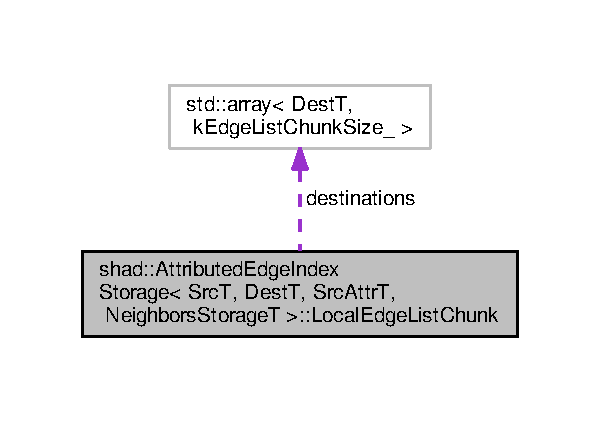
\includegraphics[width=288pt]{structshad_1_1AttributedEdgeIndexStorage_1_1LocalEdgeListChunk__coll__graph}
\end{center}
\end{figure}
\subsection*{Public Member Functions}
\begin{DoxyCompactItemize}
\item 
\hyperlink{structshad_1_1AttributedEdgeIndexStorage_1_1LocalEdgeListChunk_ac1f2e87de40eef9204e75d92ce3e48c6}{Local\-Edge\-List\-Chunk} (size\-\_\-t \-\_\-num\-Dest, bool \-\_\-ow, Dest\-T $\ast$\-\_\-dest)
\end{DoxyCompactItemize}
\subsection*{Public Attributes}
\begin{DoxyCompactItemize}
\item 
size\-\_\-t \hyperlink{structshad_1_1AttributedEdgeIndexStorage_1_1LocalEdgeListChunk_a61208febc1046cfbc776d4ba5373049b}{num\-Dest}
\item 
size\-\_\-t \hyperlink{structshad_1_1AttributedEdgeIndexStorage_1_1LocalEdgeListChunk_aa0d9a52e5792802e3f3a304fcc397eb8}{chunk\-Size}
\item 
bool \hyperlink{structshad_1_1AttributedEdgeIndexStorage_1_1LocalEdgeListChunk_af1893ff0035d04d432ff091b6c3758c0}{overwrite}
\item 
std\-::array$<$ Dest\-T, \\*
\hyperlink{classshad_1_1AttributedEdgeIndexStorage_a25f1c4ea3b8065bccaa587576d29e262}{k\-Edge\-List\-Chunk\-Size\-\_\-} $>$ \hyperlink{structshad_1_1AttributedEdgeIndexStorage_1_1LocalEdgeListChunk_a2be655891bf3c2614163b2edf8770420}{destinations}
\end{DoxyCompactItemize}


\subsection{Constructor \& Destructor Documentation}
\hypertarget{structshad_1_1AttributedEdgeIndexStorage_1_1LocalEdgeListChunk_ac1f2e87de40eef9204e75d92ce3e48c6}{\index{shad\-::\-Attributed\-Edge\-Index\-Storage\-::\-Local\-Edge\-List\-Chunk@{shad\-::\-Attributed\-Edge\-Index\-Storage\-::\-Local\-Edge\-List\-Chunk}!Local\-Edge\-List\-Chunk@{Local\-Edge\-List\-Chunk}}
\index{Local\-Edge\-List\-Chunk@{Local\-Edge\-List\-Chunk}!shad::AttributedEdgeIndexStorage::LocalEdgeListChunk@{shad\-::\-Attributed\-Edge\-Index\-Storage\-::\-Local\-Edge\-List\-Chunk}}
\subsubsection[{Local\-Edge\-List\-Chunk}]{\setlength{\rightskip}{0pt plus 5cm}template$<$typename Src\-T, typename Dest\-T, typename Src\-Attr\-T, typename Neighbors\-Storage\-T = Attr\-Edges\-Pair$<$\-Src\-Attr\-T, Dest\-T$>$$>$ {\bf shad\-::\-Attributed\-Edge\-Index\-Storage}$<$ Src\-T, Dest\-T, Src\-Attr\-T, Neighbors\-Storage\-T $>$\-::Local\-Edge\-List\-Chunk\-::\-Local\-Edge\-List\-Chunk (
\begin{DoxyParamCaption}
\item[{size\-\_\-t}]{\-\_\-num\-Dest, }
\item[{bool}]{\-\_\-ow, }
\item[{Dest\-T $\ast$}]{\-\_\-dest}
\end{DoxyParamCaption}
)\hspace{0.3cm}{\ttfamily [inline]}}}\label{structshad_1_1AttributedEdgeIndexStorage_1_1LocalEdgeListChunk_ac1f2e87de40eef9204e75d92ce3e48c6}


\subsection{Member Data Documentation}
\hypertarget{structshad_1_1AttributedEdgeIndexStorage_1_1LocalEdgeListChunk_aa0d9a52e5792802e3f3a304fcc397eb8}{\index{shad\-::\-Attributed\-Edge\-Index\-Storage\-::\-Local\-Edge\-List\-Chunk@{shad\-::\-Attributed\-Edge\-Index\-Storage\-::\-Local\-Edge\-List\-Chunk}!chunk\-Size@{chunk\-Size}}
\index{chunk\-Size@{chunk\-Size}!shad::AttributedEdgeIndexStorage::LocalEdgeListChunk@{shad\-::\-Attributed\-Edge\-Index\-Storage\-::\-Local\-Edge\-List\-Chunk}}
\subsubsection[{chunk\-Size}]{\setlength{\rightskip}{0pt plus 5cm}template$<$typename Src\-T, typename Dest\-T, typename Src\-Attr\-T, typename Neighbors\-Storage\-T = Attr\-Edges\-Pair$<$\-Src\-Attr\-T, Dest\-T$>$$>$ size\-\_\-t {\bf shad\-::\-Attributed\-Edge\-Index\-Storage}$<$ Src\-T, Dest\-T, Src\-Attr\-T, Neighbors\-Storage\-T $>$\-::Local\-Edge\-List\-Chunk\-::chunk\-Size}}\label{structshad_1_1AttributedEdgeIndexStorage_1_1LocalEdgeListChunk_aa0d9a52e5792802e3f3a304fcc397eb8}
\hypertarget{structshad_1_1AttributedEdgeIndexStorage_1_1LocalEdgeListChunk_a2be655891bf3c2614163b2edf8770420}{\index{shad\-::\-Attributed\-Edge\-Index\-Storage\-::\-Local\-Edge\-List\-Chunk@{shad\-::\-Attributed\-Edge\-Index\-Storage\-::\-Local\-Edge\-List\-Chunk}!destinations@{destinations}}
\index{destinations@{destinations}!shad::AttributedEdgeIndexStorage::LocalEdgeListChunk@{shad\-::\-Attributed\-Edge\-Index\-Storage\-::\-Local\-Edge\-List\-Chunk}}
\subsubsection[{destinations}]{\setlength{\rightskip}{0pt plus 5cm}template$<$typename Src\-T, typename Dest\-T, typename Src\-Attr\-T, typename Neighbors\-Storage\-T = Attr\-Edges\-Pair$<$\-Src\-Attr\-T, Dest\-T$>$$>$ std\-::array$<$Dest\-T, {\bf k\-Edge\-List\-Chunk\-Size\-\_\-}$>$ {\bf shad\-::\-Attributed\-Edge\-Index\-Storage}$<$ Src\-T, Dest\-T, Src\-Attr\-T, Neighbors\-Storage\-T $>$\-::Local\-Edge\-List\-Chunk\-::destinations}}\label{structshad_1_1AttributedEdgeIndexStorage_1_1LocalEdgeListChunk_a2be655891bf3c2614163b2edf8770420}
\hypertarget{structshad_1_1AttributedEdgeIndexStorage_1_1LocalEdgeListChunk_a61208febc1046cfbc776d4ba5373049b}{\index{shad\-::\-Attributed\-Edge\-Index\-Storage\-::\-Local\-Edge\-List\-Chunk@{shad\-::\-Attributed\-Edge\-Index\-Storage\-::\-Local\-Edge\-List\-Chunk}!num\-Dest@{num\-Dest}}
\index{num\-Dest@{num\-Dest}!shad::AttributedEdgeIndexStorage::LocalEdgeListChunk@{shad\-::\-Attributed\-Edge\-Index\-Storage\-::\-Local\-Edge\-List\-Chunk}}
\subsubsection[{num\-Dest}]{\setlength{\rightskip}{0pt plus 5cm}template$<$typename Src\-T, typename Dest\-T, typename Src\-Attr\-T, typename Neighbors\-Storage\-T = Attr\-Edges\-Pair$<$\-Src\-Attr\-T, Dest\-T$>$$>$ size\-\_\-t {\bf shad\-::\-Attributed\-Edge\-Index\-Storage}$<$ Src\-T, Dest\-T, Src\-Attr\-T, Neighbors\-Storage\-T $>$\-::Local\-Edge\-List\-Chunk\-::num\-Dest}}\label{structshad_1_1AttributedEdgeIndexStorage_1_1LocalEdgeListChunk_a61208febc1046cfbc776d4ba5373049b}
\hypertarget{structshad_1_1AttributedEdgeIndexStorage_1_1LocalEdgeListChunk_af1893ff0035d04d432ff091b6c3758c0}{\index{shad\-::\-Attributed\-Edge\-Index\-Storage\-::\-Local\-Edge\-List\-Chunk@{shad\-::\-Attributed\-Edge\-Index\-Storage\-::\-Local\-Edge\-List\-Chunk}!overwrite@{overwrite}}
\index{overwrite@{overwrite}!shad::AttributedEdgeIndexStorage::LocalEdgeListChunk@{shad\-::\-Attributed\-Edge\-Index\-Storage\-::\-Local\-Edge\-List\-Chunk}}
\subsubsection[{overwrite}]{\setlength{\rightskip}{0pt plus 5cm}template$<$typename Src\-T, typename Dest\-T, typename Src\-Attr\-T, typename Neighbors\-Storage\-T = Attr\-Edges\-Pair$<$\-Src\-Attr\-T, Dest\-T$>$$>$ bool {\bf shad\-::\-Attributed\-Edge\-Index\-Storage}$<$ Src\-T, Dest\-T, Src\-Attr\-T, Neighbors\-Storage\-T $>$\-::Local\-Edge\-List\-Chunk\-::overwrite}}\label{structshad_1_1AttributedEdgeIndexStorage_1_1LocalEdgeListChunk_af1893ff0035d04d432ff091b6c3758c0}


The documentation for this struct was generated from the following file\-:\begin{DoxyCompactItemize}
\item 
include/shad/extensions/graph\-\_\-library/\hyperlink{attributed__edge__index_8h}{attributed\-\_\-edge\-\_\-index.\-h}\end{DoxyCompactItemize}

\hypertarget{structshad_1_1DefaultEdgeIndexStorage_1_1LocalEdgeListChunk}{\section{shad\-:\-:Default\-Edge\-Index\-Storage$<$ Src\-T, Dest\-T, Neighbors\-Storage\-T $>$\-:\-:Local\-Edge\-List\-Chunk Struct Reference}
\label{structshad_1_1DefaultEdgeIndexStorage_1_1LocalEdgeListChunk}\index{shad\-::\-Default\-Edge\-Index\-Storage$<$ Src\-T, Dest\-T, Neighbors\-Storage\-T $>$\-::\-Local\-Edge\-List\-Chunk@{shad\-::\-Default\-Edge\-Index\-Storage$<$ Src\-T, Dest\-T, Neighbors\-Storage\-T $>$\-::\-Local\-Edge\-List\-Chunk}}
}


{\ttfamily \#include $<$shad/extensions/graph\-\_\-library/local\-\_\-edge\-\_\-index.\-h$>$}



Collaboration diagram for shad\-:\-:Default\-Edge\-Index\-Storage$<$ Src\-T, Dest\-T, Neighbors\-Storage\-T $>$\-:\-:Local\-Edge\-List\-Chunk\-:
\nopagebreak
\begin{figure}[H]
\begin{center}
\leavevmode
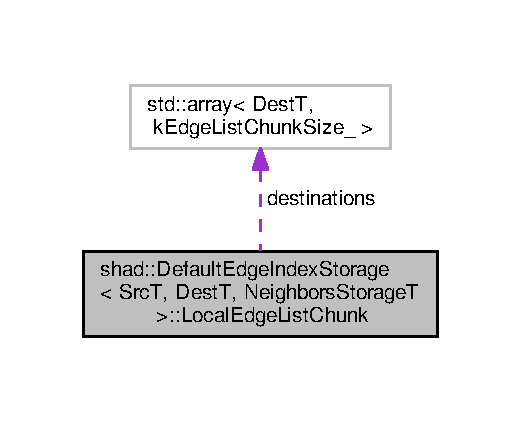
\includegraphics[width=250pt]{structshad_1_1DefaultEdgeIndexStorage_1_1LocalEdgeListChunk__coll__graph}
\end{center}
\end{figure}
\subsection*{Public Member Functions}
\begin{DoxyCompactItemize}
\item 
\hyperlink{structshad_1_1DefaultEdgeIndexStorage_1_1LocalEdgeListChunk_a536a899e890ea5b51805efbf4c5ab8d6}{Local\-Edge\-List\-Chunk} (size\-\_\-t \-\_\-num\-Dest, bool \-\_\-ow, Dest\-T $\ast$\-\_\-dest)
\end{DoxyCompactItemize}
\subsection*{Public Attributes}
\begin{DoxyCompactItemize}
\item 
size\-\_\-t \hyperlink{structshad_1_1DefaultEdgeIndexStorage_1_1LocalEdgeListChunk_a3091dc3831cae7d0dcc7ab1b53141225}{num\-Dest}
\item 
size\-\_\-t \hyperlink{structshad_1_1DefaultEdgeIndexStorage_1_1LocalEdgeListChunk_a6d82addc7d5c342822104d750afec0c9}{chunk\-Size}
\item 
bool \hyperlink{structshad_1_1DefaultEdgeIndexStorage_1_1LocalEdgeListChunk_af16ee8a11ee5912e40703608767038e3}{overwrite}
\item 
std\-::array$<$ Dest\-T, \\*
\hyperlink{classshad_1_1DefaultEdgeIndexStorage_aae9f28f3799a6a274b0249dc1dc4313c}{k\-Edge\-List\-Chunk\-Size\-\_\-} $>$ \hyperlink{structshad_1_1DefaultEdgeIndexStorage_1_1LocalEdgeListChunk_adc9b9bf8d3bd6c3adb394737e3038907}{destinations}
\end{DoxyCompactItemize}


\subsection{Constructor \& Destructor Documentation}
\hypertarget{structshad_1_1DefaultEdgeIndexStorage_1_1LocalEdgeListChunk_a536a899e890ea5b51805efbf4c5ab8d6}{\index{shad\-::\-Default\-Edge\-Index\-Storage\-::\-Local\-Edge\-List\-Chunk@{shad\-::\-Default\-Edge\-Index\-Storage\-::\-Local\-Edge\-List\-Chunk}!Local\-Edge\-List\-Chunk@{Local\-Edge\-List\-Chunk}}
\index{Local\-Edge\-List\-Chunk@{Local\-Edge\-List\-Chunk}!shad::DefaultEdgeIndexStorage::LocalEdgeListChunk@{shad\-::\-Default\-Edge\-Index\-Storage\-::\-Local\-Edge\-List\-Chunk}}
\subsubsection[{Local\-Edge\-List\-Chunk}]{\setlength{\rightskip}{0pt plus 5cm}template$<$typename Src\-T, typename Dest\-T, typename Neighbors\-Storage\-T = Local\-Set$<$\-Dest\-T$>$$>$ {\bf shad\-::\-Default\-Edge\-Index\-Storage}$<$ Src\-T, Dest\-T, Neighbors\-Storage\-T $>$\-::Local\-Edge\-List\-Chunk\-::\-Local\-Edge\-List\-Chunk (
\begin{DoxyParamCaption}
\item[{size\-\_\-t}]{\-\_\-num\-Dest, }
\item[{bool}]{\-\_\-ow, }
\item[{Dest\-T $\ast$}]{\-\_\-dest}
\end{DoxyParamCaption}
)\hspace{0.3cm}{\ttfamily [inline]}}}\label{structshad_1_1DefaultEdgeIndexStorage_1_1LocalEdgeListChunk_a536a899e890ea5b51805efbf4c5ab8d6}


\subsection{Member Data Documentation}
\hypertarget{structshad_1_1DefaultEdgeIndexStorage_1_1LocalEdgeListChunk_a6d82addc7d5c342822104d750afec0c9}{\index{shad\-::\-Default\-Edge\-Index\-Storage\-::\-Local\-Edge\-List\-Chunk@{shad\-::\-Default\-Edge\-Index\-Storage\-::\-Local\-Edge\-List\-Chunk}!chunk\-Size@{chunk\-Size}}
\index{chunk\-Size@{chunk\-Size}!shad::DefaultEdgeIndexStorage::LocalEdgeListChunk@{shad\-::\-Default\-Edge\-Index\-Storage\-::\-Local\-Edge\-List\-Chunk}}
\subsubsection[{chunk\-Size}]{\setlength{\rightskip}{0pt plus 5cm}template$<$typename Src\-T, typename Dest\-T, typename Neighbors\-Storage\-T = Local\-Set$<$\-Dest\-T$>$$>$ size\-\_\-t {\bf shad\-::\-Default\-Edge\-Index\-Storage}$<$ Src\-T, Dest\-T, Neighbors\-Storage\-T $>$\-::Local\-Edge\-List\-Chunk\-::chunk\-Size}}\label{structshad_1_1DefaultEdgeIndexStorage_1_1LocalEdgeListChunk_a6d82addc7d5c342822104d750afec0c9}
\hypertarget{structshad_1_1DefaultEdgeIndexStorage_1_1LocalEdgeListChunk_adc9b9bf8d3bd6c3adb394737e3038907}{\index{shad\-::\-Default\-Edge\-Index\-Storage\-::\-Local\-Edge\-List\-Chunk@{shad\-::\-Default\-Edge\-Index\-Storage\-::\-Local\-Edge\-List\-Chunk}!destinations@{destinations}}
\index{destinations@{destinations}!shad::DefaultEdgeIndexStorage::LocalEdgeListChunk@{shad\-::\-Default\-Edge\-Index\-Storage\-::\-Local\-Edge\-List\-Chunk}}
\subsubsection[{destinations}]{\setlength{\rightskip}{0pt plus 5cm}template$<$typename Src\-T, typename Dest\-T, typename Neighbors\-Storage\-T = Local\-Set$<$\-Dest\-T$>$$>$ std\-::array$<$Dest\-T, {\bf k\-Edge\-List\-Chunk\-Size\-\_\-}$>$ {\bf shad\-::\-Default\-Edge\-Index\-Storage}$<$ Src\-T, Dest\-T, Neighbors\-Storage\-T $>$\-::Local\-Edge\-List\-Chunk\-::destinations}}\label{structshad_1_1DefaultEdgeIndexStorage_1_1LocalEdgeListChunk_adc9b9bf8d3bd6c3adb394737e3038907}
\hypertarget{structshad_1_1DefaultEdgeIndexStorage_1_1LocalEdgeListChunk_a3091dc3831cae7d0dcc7ab1b53141225}{\index{shad\-::\-Default\-Edge\-Index\-Storage\-::\-Local\-Edge\-List\-Chunk@{shad\-::\-Default\-Edge\-Index\-Storage\-::\-Local\-Edge\-List\-Chunk}!num\-Dest@{num\-Dest}}
\index{num\-Dest@{num\-Dest}!shad::DefaultEdgeIndexStorage::LocalEdgeListChunk@{shad\-::\-Default\-Edge\-Index\-Storage\-::\-Local\-Edge\-List\-Chunk}}
\subsubsection[{num\-Dest}]{\setlength{\rightskip}{0pt plus 5cm}template$<$typename Src\-T, typename Dest\-T, typename Neighbors\-Storage\-T = Local\-Set$<$\-Dest\-T$>$$>$ size\-\_\-t {\bf shad\-::\-Default\-Edge\-Index\-Storage}$<$ Src\-T, Dest\-T, Neighbors\-Storage\-T $>$\-::Local\-Edge\-List\-Chunk\-::num\-Dest}}\label{structshad_1_1DefaultEdgeIndexStorage_1_1LocalEdgeListChunk_a3091dc3831cae7d0dcc7ab1b53141225}
\hypertarget{structshad_1_1DefaultEdgeIndexStorage_1_1LocalEdgeListChunk_af16ee8a11ee5912e40703608767038e3}{\index{shad\-::\-Default\-Edge\-Index\-Storage\-::\-Local\-Edge\-List\-Chunk@{shad\-::\-Default\-Edge\-Index\-Storage\-::\-Local\-Edge\-List\-Chunk}!overwrite@{overwrite}}
\index{overwrite@{overwrite}!shad::DefaultEdgeIndexStorage::LocalEdgeListChunk@{shad\-::\-Default\-Edge\-Index\-Storage\-::\-Local\-Edge\-List\-Chunk}}
\subsubsection[{overwrite}]{\setlength{\rightskip}{0pt plus 5cm}template$<$typename Src\-T, typename Dest\-T, typename Neighbors\-Storage\-T = Local\-Set$<$\-Dest\-T$>$$>$ bool {\bf shad\-::\-Default\-Edge\-Index\-Storage}$<$ Src\-T, Dest\-T, Neighbors\-Storage\-T $>$\-::Local\-Edge\-List\-Chunk\-::overwrite}}\label{structshad_1_1DefaultEdgeIndexStorage_1_1LocalEdgeListChunk_af16ee8a11ee5912e40703608767038e3}


The documentation for this struct was generated from the following file\-:\begin{DoxyCompactItemize}
\item 
include/shad/extensions/graph\-\_\-library/\hyperlink{local__edge__index_8h}{local\-\_\-edge\-\_\-index.\-h}\end{DoxyCompactItemize}

\hypertarget{classshad_1_1LocalHashmap}{\section{shad\-:\-:Local\-Hashmap$<$ K\-T\-Y\-P\-E, V\-T\-Y\-P\-E, K\-E\-Y\-\_\-\-C\-O\-M\-P\-A\-R\-E, I\-N\-S\-E\-R\-T\-E\-R $>$ Class Template Reference}
\label{classshad_1_1LocalHashmap}\index{shad\-::\-Local\-Hashmap$<$ K\-T\-Y\-P\-E, V\-T\-Y\-P\-E, K\-E\-Y\-\_\-\-C\-O\-M\-P\-A\-R\-E, I\-N\-S\-E\-R\-T\-E\-R $>$@{shad\-::\-Local\-Hashmap$<$ K\-T\-Y\-P\-E, V\-T\-Y\-P\-E, K\-E\-Y\-\_\-\-C\-O\-M\-P\-A\-R\-E, I\-N\-S\-E\-R\-T\-E\-R $>$}}
}


The \hyperlink{classshad_1_1LocalHashmap}{Local\-Hashmap} data structure.  




{\ttfamily \#include $<$shad/data\-\_\-structures/local\-\_\-hashmap.\-h$>$}

\subsection*{Classes}
\begin{DoxyCompactItemize}
\item 
struct \hyperlink{structshad_1_1LocalHashmap_1_1LookupResult}{Lookup\-Result}
\begin{DoxyCompactList}\small\item\em Result for the \hyperlink{classshad_1_1LocalHashmap_a9bd1b3780c1c676ce8d5eae265030080}{Lookup(const K\-T\-Y\-P\-E\&, Lookup\-Result$\ast$)} and \hyperlink{classshad_1_1LocalHashmap_a0328e22adb5dd53e819cc1791e802a56}{Async\-Lookup(rt\-::\-Handle\&, const K\-T\-Y\-P\-E\&, Lookup\-Result$\ast$)} methods. \end{DoxyCompactList}\end{DoxyCompactItemize}
\subsection*{Public Types}
\begin{DoxyCompactItemize}
\item 
using \hyperlink{classshad_1_1LocalHashmap_a3fa27c320a046745e01804325f15dd0e}{value\-\_\-type} = std\-::pair$<$ K\-T\-Y\-P\-E, V\-T\-Y\-P\-E $>$
\item 
using \hyperlink{classshad_1_1LocalHashmap_a130dbe16edd42ee7aa2e27eac6ee3cf4}{iterator} = \hyperlink{classshad_1_1lmap__iterator}{lmap\-\_\-iterator}$<$ \hyperlink{classshad_1_1LocalHashmap}{Local\-Hashmap}$<$ K\-T\-Y\-P\-E, V\-T\-Y\-P\-E, K\-E\-Y\-\_\-\-C\-O\-M\-P\-A\-R\-E, I\-N\-S\-E\-R\-T\-E\-R $>$, std\-::pair$<$ K\-T\-Y\-P\-E, V\-T\-Y\-P\-E $>$$>$
\item 
using \hyperlink{classshad_1_1LocalHashmap_ad5e054bdbc20f161cd8df8e00c525401}{const\-\_\-iterator} = \hyperlink{classshad_1_1lmap__iterator}{lmap\-\_\-iterator}$<$ \hyperlink{classshad_1_1LocalHashmap}{Local\-Hashmap}$<$ K\-T\-Y\-P\-E, V\-T\-Y\-P\-E, K\-E\-Y\-\_\-\-C\-O\-M\-P\-A\-R\-E, I\-N\-S\-E\-R\-T\-E\-R $>$, const std\-::pair$<$ K\-T\-Y\-P\-E, V\-T\-Y\-P\-E $>$$>$
\end{DoxyCompactItemize}
\subsection*{Public Member Functions}
\begin{DoxyCompactItemize}
\item 
\hyperlink{classshad_1_1LocalHashmap_a6c0ce5d7583545126171e9de452b89d9}{Local\-Hashmap} (const size\-\_\-t num\-Init\-Buckets)
\begin{DoxyCompactList}\small\item\em Constructor. \end{DoxyCompactList}\item 
size\-\_\-t \hyperlink{classshad_1_1LocalHashmap_ac70c307f612b97f08f5e38bba7759665}{Size} () const 
\begin{DoxyCompactList}\small\item\em Size of the hashmap (number of entries). \end{DoxyCompactList}\item 
V\-T\-Y\-P\-E $\ast$ \hyperlink{classshad_1_1LocalHashmap_af3ef8afed1593bf034477b8692661b97}{Insert} (const K\-T\-Y\-P\-E \&key, const V\-T\-Y\-P\-E \&value)
\begin{DoxyCompactList}\small\item\em Insert a key-\/value pair in the hashmap. \end{DoxyCompactList}\item 
{\footnotesize template$<$typename E\-L\-T\-Y\-P\-E $>$ }\\V\-T\-Y\-P\-E $\ast$ \hyperlink{classshad_1_1LocalHashmap_ad8062ff16023002c7aee667f3fe4cfd2}{Insert} (const K\-T\-Y\-P\-E \&key, const E\-L\-T\-Y\-P\-E \&value)
\item 
void \hyperlink{classshad_1_1LocalHashmap_acb5581492e044c07bd0ceaa3a6892309}{Async\-Insert} (\hyperlink{classshad_1_1rt_1_1Handle}{rt\-::\-Handle} \&handle, const K\-T\-Y\-P\-E \&key, const V\-T\-Y\-P\-E \&value)
\begin{DoxyCompactList}\small\item\em Asynchronously Insert a key-\/value pair in the hashmap. \end{DoxyCompactList}\item 
{\footnotesize template$<$typename E\-L\-T\-Y\-P\-E $>$ }\\void \hyperlink{classshad_1_1LocalHashmap_ace0dd4d4a9caee1d915af6efcb4fc2c6}{Async\-Insert} (\hyperlink{classshad_1_1rt_1_1Handle}{rt\-::\-Handle} \&handle, const K\-T\-Y\-P\-E \&key, const E\-L\-T\-Y\-P\-E \&value)
\item 
void \hyperlink{classshad_1_1LocalHashmap_a5d57f63d0515acf2d53c99fb56eda93c}{Erase} (const K\-T\-Y\-P\-E \&key)
\begin{DoxyCompactList}\small\item\em Remove a key-\/value pair from the hashmap. \end{DoxyCompactList}\item 
void \hyperlink{classshad_1_1LocalHashmap_a78d00a5d4b2591cefcafb44247d9131d}{Async\-Erase} (\hyperlink{classshad_1_1rt_1_1Handle}{rt\-::\-Handle} \&handle, const K\-T\-Y\-P\-E \&key)
\begin{DoxyCompactList}\small\item\em Asynchronously remove a key-\/value pair from the hashmap. \end{DoxyCompactList}\item 
void \hyperlink{classshad_1_1LocalHashmap_a4e95baa9af6646d2c66adc1b8ae5781c}{Clear} ()
\begin{DoxyCompactList}\small\item\em Clear the content of the hashmap. \end{DoxyCompactList}\item 
bool \hyperlink{classshad_1_1LocalHashmap_a0365f5c68c75b04109639e8f65cc8eb0}{Lookup} (const K\-T\-Y\-P\-E \&key, V\-T\-Y\-P\-E $\ast$res)
\begin{DoxyCompactList}\small\item\em Get the value associated to a key. \end{DoxyCompactList}\item 
V\-T\-Y\-P\-E $\ast$ \hyperlink{classshad_1_1LocalHashmap_ae37645e79a683b4bc8c096a37cacf74d}{Lookup} (const K\-T\-Y\-P\-E \&key)
\begin{DoxyCompactList}\small\item\em Get the value associated to a key. \end{DoxyCompactList}\item 
void \hyperlink{classshad_1_1LocalHashmap_ab80af4eef1ce16673c1895bd6cd3951b}{Async\-Lookup} (\hyperlink{classshad_1_1rt_1_1Handle}{rt\-::\-Handle} \&handle, const K\-T\-Y\-P\-E \&key, V\-T\-Y\-P\-E $\ast$$\ast$res)
\begin{DoxyCompactList}\small\item\em Asynchronously get the value associated to a key. \end{DoxyCompactList}\item 
void \hyperlink{classshad_1_1LocalHashmap_a9bd1b3780c1c676ce8d5eae265030080}{Lookup} (const K\-T\-Y\-P\-E \&key, \hyperlink{structshad_1_1LocalHashmap_1_1LookupResult}{Lookup\-Result} $\ast$res)
\begin{DoxyCompactList}\small\item\em Lookup method. \end{DoxyCompactList}\item 
void \hyperlink{classshad_1_1LocalHashmap_a0328e22adb5dd53e819cc1791e802a56}{Async\-Lookup} (\hyperlink{classshad_1_1rt_1_1Handle}{rt\-::\-Handle} \&handle, const K\-T\-Y\-P\-E \&key, \hyperlink{structshad_1_1LocalHashmap_1_1LookupResult}{Lookup\-Result} $\ast$res)
\begin{DoxyCompactList}\small\item\em Asynchronous lookup method. \end{DoxyCompactList}\item 
{\footnotesize template$<$typename Apply\-Fun\-T , typename... Args$>$ }\\void \hyperlink{classshad_1_1LocalHashmap_aa95a9226e3f63dbe5ce08593552175fe}{Apply} (const K\-T\-Y\-P\-E \&key, Apply\-Fun\-T \&\&function, Args \&...args)
\begin{DoxyCompactList}\small\item\em Apply a user-\/defined function to a key-\/value pair. \end{DoxyCompactList}\item 
{\footnotesize template$<$typename Apply\-Fun\-T , typename... Args$>$ }\\void \hyperlink{classshad_1_1LocalHashmap_a359f3fae23cbb8c4548d6abe0047ac9b}{Async\-Apply} (\hyperlink{classshad_1_1rt_1_1Handle}{rt\-::\-Handle} \&handle, const K\-T\-Y\-P\-E \&key, Apply\-Fun\-T \&\&function, Args \&...args)
\begin{DoxyCompactList}\small\item\em Asynchronously apply a user-\/defined function to a key-\/value pair. \end{DoxyCompactList}\item 
{\footnotesize template$<$typename Apply\-Fun\-T , typename... Args$>$ }\\void \hyperlink{classshad_1_1LocalHashmap_a0532b7cb7bd734295e18699a00dc8998}{For\-Each\-Entry} (Apply\-Fun\-T \&\&function, Args \&...args)
\begin{DoxyCompactList}\small\item\em Apply a user-\/defined function to each key-\/value pair. \end{DoxyCompactList}\item 
{\footnotesize template$<$typename Apply\-Fun\-T , typename... Args$>$ }\\void \hyperlink{classshad_1_1LocalHashmap_a82d24ff551ababdabb0d50e6c7827c0a}{Async\-For\-Each\-Entry} (\hyperlink{classshad_1_1rt_1_1Handle}{rt\-::\-Handle} \&handle, Apply\-Fun\-T \&\&function, Args \&...args)
\begin{DoxyCompactList}\small\item\em Asynchronously apply a user-\/defined function to each key-\/value pair. \end{DoxyCompactList}\item 
{\footnotesize template$<$typename Apply\-Fun\-T , typename... Args$>$ }\\void \hyperlink{classshad_1_1LocalHashmap_af8308e042d3b4a435517404ca4679d82}{For\-Each\-Key} (Apply\-Fun\-T \&\&function, Args \&...args)
\begin{DoxyCompactList}\small\item\em Apply a user-\/defined function to each key. \end{DoxyCompactList}\item 
{\footnotesize template$<$typename Apply\-Fun\-T , typename... Args$>$ }\\void \hyperlink{classshad_1_1LocalHashmap_a559f24258bb798fdfafbb28fc70ccbd8}{Async\-For\-Each\-Key} (\hyperlink{classshad_1_1rt_1_1Handle}{rt\-::\-Handle} \&handle, Apply\-Fun\-T \&\&function, Args \&...args)
\begin{DoxyCompactList}\small\item\em Asynchronously apply a user-\/defined function to each key. \end{DoxyCompactList}\item 
void \hyperlink{classshad_1_1LocalHashmap_a7dc7ac304876af70108a24c7b82d408e}{Print\-All\-Entries} ()
\begin{DoxyCompactList}\small\item\em Print all the entries in the hashmap. \end{DoxyCompactList}\item 
\hyperlink{classshad_1_1LocalHashmap_a130dbe16edd42ee7aa2e27eac6ee3cf4}{iterator} \hyperlink{classshad_1_1LocalHashmap_ad84d91d8fd4448a2017b39480c842984}{begin} ()
\item 
\hyperlink{classshad_1_1LocalHashmap_a130dbe16edd42ee7aa2e27eac6ee3cf4}{iterator} \hyperlink{classshad_1_1LocalHashmap_a6171d13fb3d6d493068e23cd166e8929}{end} ()
\item 
\hyperlink{classshad_1_1LocalHashmap_ad5e054bdbc20f161cd8df8e00c525401}{const\-\_\-iterator} \hyperlink{classshad_1_1LocalHashmap_a9cc4e9135d4808fbf53f253755744019}{cbegin} ()
\item 
\hyperlink{classshad_1_1LocalHashmap_ad5e054bdbc20f161cd8df8e00c525401}{const\-\_\-iterator} \hyperlink{classshad_1_1LocalHashmap_a18da968a5c684f5b4abbdd0bf6760574}{cend} ()
\end{DoxyCompactItemize}
\subsection*{Friends}
\begin{DoxyCompactItemize}
\item 
{\footnotesize template$<$typename , typename , typename , typename $>$ }\\class \hyperlink{classshad_1_1LocalHashmap_a14c7f14e3d86371810686e384b53cbb6}{Hashmap}
\item 
class \hyperlink{classshad_1_1LocalHashmap_a0782f66aa59afb708b15c0ef7782c20d}{lmap\-\_\-iterator$<$ Local\-Hashmap$<$ K\-T\-Y\-P\-E, V\-T\-Y\-P\-E, K\-E\-Y\-\_\-\-C\-O\-M\-P\-A\-R\-E, I\-N\-S\-E\-R\-T\-E\-R $>$, std\-::pair$<$ K\-T\-Y\-P\-E, V\-T\-Y\-P\-E $>$ $>$}
\item 
class \hyperlink{classshad_1_1LocalHashmap_a409d20941abf9e3ce2b3f49f749fe1f7}{lmap\-\_\-iterator$<$ Local\-Hashmap$<$ K\-T\-Y\-P\-E, V\-T\-Y\-P\-E, K\-E\-Y\-\_\-\-C\-O\-M\-P\-A\-R\-E, I\-N\-S\-E\-R\-T\-E\-R $>$, const std\-::pair$<$ K\-T\-Y\-P\-E, V\-T\-Y\-P\-E $>$ $>$}
\item 
{\footnotesize template$<$typename , typename , typename $>$ }\\class \hyperlink{classshad_1_1LocalHashmap_ae4a075e5a8191685a74f2d18b8cd8850}{map\-\_\-iterator}
\end{DoxyCompactItemize}


\subsection{Detailed Description}
\subsubsection*{template$<$typename K\-T\-Y\-P\-E, typename V\-T\-Y\-P\-E, typename K\-E\-Y\-\_\-\-C\-O\-M\-P\-A\-R\-E = Mem\-Cmp$<$\-K\-T\-Y\-P\-E$>$, typename I\-N\-S\-E\-R\-T\-E\-R = Overwriter$<$\-V\-T\-Y\-P\-E$>$$>$class shad\-::\-Local\-Hashmap$<$ K\-T\-Y\-P\-E, V\-T\-Y\-P\-E, K\-E\-Y\-\_\-\-C\-O\-M\-P\-A\-R\-E, I\-N\-S\-E\-R\-T\-E\-R $>$}

The \hyperlink{classshad_1_1LocalHashmap}{Local\-Hashmap} data structure. 

S\-H\-A\-D's \hyperlink{classshad_1_1LocalHashmap}{Local\-Hashmap} is a \char`\"{}local\char`\"{}, thread-\/safe, associative container. Local\-Hashmaps can be used O\-N\-L\-Y on the Locality on which they are created. 
\begin{DoxyTemplParams}{Template Parameters}
{\em K\-T\-Y\-P\-E} & type of the hashmap keys. \\
\hline
{\em V\-T\-Y\-P\-E} & type of the hashmap values. \\
\hline
{\em K\-E\-Y\-\_\-\-C\-O\-M\-P\-A\-R\-E} & key comparison function; default is Mem\-Cmp$<$\-K\-T\-Y\-P\-E$>$. \\
\hline
{\em I\-N\-S\-E\-R\-T\-E\-R} & default is \hyperlink{structshad_1_1Overwriter}{Overwriter} (i.\-e. insertions overwrite previous values associated to the same key, if any). \\
\hline
\end{DoxyTemplParams}


\subsection{Member Typedef Documentation}
\hypertarget{classshad_1_1LocalHashmap_ad5e054bdbc20f161cd8df8e00c525401}{\index{shad\-::\-Local\-Hashmap@{shad\-::\-Local\-Hashmap}!const\-\_\-iterator@{const\-\_\-iterator}}
\index{const\-\_\-iterator@{const\-\_\-iterator}!shad::LocalHashmap@{shad\-::\-Local\-Hashmap}}
\subsubsection[{const\-\_\-iterator}]{\setlength{\rightskip}{0pt plus 5cm}template$<$typename K\-T\-Y\-P\-E, typename V\-T\-Y\-P\-E, typename K\-E\-Y\-\_\-\-C\-O\-M\-P\-A\-R\-E = Mem\-Cmp$<$\-K\-T\-Y\-P\-E$>$, typename I\-N\-S\-E\-R\-T\-E\-R = Overwriter$<$\-V\-T\-Y\-P\-E$>$$>$ using {\bf shad\-::\-Local\-Hashmap}$<$ K\-T\-Y\-P\-E, V\-T\-Y\-P\-E, K\-E\-Y\-\_\-\-C\-O\-M\-P\-A\-R\-E, I\-N\-S\-E\-R\-T\-E\-R $>$\-::{\bf const\-\_\-iterator} =  {\bf lmap\-\_\-iterator}$<${\bf Local\-Hashmap}$<$K\-T\-Y\-P\-E, V\-T\-Y\-P\-E, K\-E\-Y\-\_\-\-C\-O\-M\-P\-A\-R\-E, I\-N\-S\-E\-R\-T\-E\-R$>$, const std\-::pair$<$K\-T\-Y\-P\-E, V\-T\-Y\-P\-E$>$$>$}}\label{classshad_1_1LocalHashmap_ad5e054bdbc20f161cd8df8e00c525401}
\hypertarget{classshad_1_1LocalHashmap_a130dbe16edd42ee7aa2e27eac6ee3cf4}{\index{shad\-::\-Local\-Hashmap@{shad\-::\-Local\-Hashmap}!iterator@{iterator}}
\index{iterator@{iterator}!shad::LocalHashmap@{shad\-::\-Local\-Hashmap}}
\subsubsection[{iterator}]{\setlength{\rightskip}{0pt plus 5cm}template$<$typename K\-T\-Y\-P\-E, typename V\-T\-Y\-P\-E, typename K\-E\-Y\-\_\-\-C\-O\-M\-P\-A\-R\-E = Mem\-Cmp$<$\-K\-T\-Y\-P\-E$>$, typename I\-N\-S\-E\-R\-T\-E\-R = Overwriter$<$\-V\-T\-Y\-P\-E$>$$>$ using {\bf shad\-::\-Local\-Hashmap}$<$ K\-T\-Y\-P\-E, V\-T\-Y\-P\-E, K\-E\-Y\-\_\-\-C\-O\-M\-P\-A\-R\-E, I\-N\-S\-E\-R\-T\-E\-R $>$\-::{\bf iterator} =  {\bf lmap\-\_\-iterator}$<${\bf Local\-Hashmap}$<$K\-T\-Y\-P\-E, V\-T\-Y\-P\-E, K\-E\-Y\-\_\-\-C\-O\-M\-P\-A\-R\-E, I\-N\-S\-E\-R\-T\-E\-R$>$, std\-::pair$<$K\-T\-Y\-P\-E, V\-T\-Y\-P\-E$>$$>$}}\label{classshad_1_1LocalHashmap_a130dbe16edd42ee7aa2e27eac6ee3cf4}
\hypertarget{classshad_1_1LocalHashmap_a3fa27c320a046745e01804325f15dd0e}{\index{shad\-::\-Local\-Hashmap@{shad\-::\-Local\-Hashmap}!value\-\_\-type@{value\-\_\-type}}
\index{value\-\_\-type@{value\-\_\-type}!shad::LocalHashmap@{shad\-::\-Local\-Hashmap}}
\subsubsection[{value\-\_\-type}]{\setlength{\rightskip}{0pt plus 5cm}template$<$typename K\-T\-Y\-P\-E, typename V\-T\-Y\-P\-E, typename K\-E\-Y\-\_\-\-C\-O\-M\-P\-A\-R\-E = Mem\-Cmp$<$\-K\-T\-Y\-P\-E$>$, typename I\-N\-S\-E\-R\-T\-E\-R = Overwriter$<$\-V\-T\-Y\-P\-E$>$$>$ using {\bf shad\-::\-Local\-Hashmap}$<$ K\-T\-Y\-P\-E, V\-T\-Y\-P\-E, K\-E\-Y\-\_\-\-C\-O\-M\-P\-A\-R\-E, I\-N\-S\-E\-R\-T\-E\-R $>$\-::{\bf value\-\_\-type} =  std\-::pair$<$K\-T\-Y\-P\-E, V\-T\-Y\-P\-E$>$}}\label{classshad_1_1LocalHashmap_a3fa27c320a046745e01804325f15dd0e}


\subsection{Constructor \& Destructor Documentation}
\hypertarget{classshad_1_1LocalHashmap_a6c0ce5d7583545126171e9de452b89d9}{\index{shad\-::\-Local\-Hashmap@{shad\-::\-Local\-Hashmap}!Local\-Hashmap@{Local\-Hashmap}}
\index{Local\-Hashmap@{Local\-Hashmap}!shad::LocalHashmap@{shad\-::\-Local\-Hashmap}}
\subsubsection[{Local\-Hashmap}]{\setlength{\rightskip}{0pt plus 5cm}template$<$typename K\-T\-Y\-P\-E, typename V\-T\-Y\-P\-E, typename K\-E\-Y\-\_\-\-C\-O\-M\-P\-A\-R\-E = Mem\-Cmp$<$\-K\-T\-Y\-P\-E$>$, typename I\-N\-S\-E\-R\-T\-E\-R = Overwriter$<$\-V\-T\-Y\-P\-E$>$$>$ {\bf shad\-::\-Local\-Hashmap}$<$ K\-T\-Y\-P\-E, V\-T\-Y\-P\-E, K\-E\-Y\-\_\-\-C\-O\-M\-P\-A\-R\-E, I\-N\-S\-E\-R\-T\-E\-R $>$\-::{\bf Local\-Hashmap} (
\begin{DoxyParamCaption}
\item[{const size\-\_\-t}]{num\-Init\-Buckets}
\end{DoxyParamCaption}
)\hspace{0.3cm}{\ttfamily [inline]}, {\ttfamily [explicit]}}}\label{classshad_1_1LocalHashmap_a6c0ce5d7583545126171e9de452b89d9}


Constructor. 


\begin{DoxyParams}{Parameters}
{\em num\-Init\-Buckets} & initial number of Buckets. \\
\hline
\end{DoxyParams}


\subsection{Member Function Documentation}
\hypertarget{classshad_1_1LocalHashmap_aa95a9226e3f63dbe5ce08593552175fe}{\index{shad\-::\-Local\-Hashmap@{shad\-::\-Local\-Hashmap}!Apply@{Apply}}
\index{Apply@{Apply}!shad::LocalHashmap@{shad\-::\-Local\-Hashmap}}
\subsubsection[{Apply}]{\setlength{\rightskip}{0pt plus 5cm}template$<$typename K\-T\-Y\-P\-E, typename V\-T\-Y\-P\-E, typename K\-E\-Y\-\_\-\-C\-O\-M\-P\-A\-R\-E = Mem\-Cmp$<$\-K\-T\-Y\-P\-E$>$, typename I\-N\-S\-E\-R\-T\-E\-R = Overwriter$<$\-V\-T\-Y\-P\-E$>$$>$ template$<$typename Apply\-Fun\-T , typename... Args$>$ void {\bf shad\-::\-Local\-Hashmap}$<$ K\-T\-Y\-P\-E, V\-T\-Y\-P\-E, K\-E\-Y\-\_\-\-C\-O\-M\-P\-A\-R\-E, I\-N\-S\-E\-R\-T\-E\-R $>$\-::Apply (
\begin{DoxyParamCaption}
\item[{const K\-T\-Y\-P\-E \&}]{key, }
\item[{Apply\-Fun\-T \&\&}]{function, }
\item[{Args \&...}]{args}
\end{DoxyParamCaption}
)\hspace{0.3cm}{\ttfamily [inline]}}}\label{classshad_1_1LocalHashmap_aa95a9226e3f63dbe5ce08593552175fe}


Apply a user-\/defined function to a key-\/value pair. 


\begin{DoxyTemplParams}{Template Parameters}
{\em Apply\-Fun\-T} & User-\/defined function type. The function prototype should be\-: 
\begin{DoxyCode}
void(\textcolor{keyword}{const} KTYPE&, VTYPE&, Args&);
\end{DoxyCode}
 \\
\hline
{\em ...\-Args} & Types of the function arguments.\\
\hline
\end{DoxyTemplParams}

\begin{DoxyParams}[1]{Parameters}
\mbox{\tt in}  & {\em key} & The key. \\
\hline
 & {\em function} & The function to apply. \\
\hline
 & {\em args} & The function arguments. \\
\hline
\end{DoxyParams}
\hypertarget{classshad_1_1LocalHashmap_a359f3fae23cbb8c4548d6abe0047ac9b}{\index{shad\-::\-Local\-Hashmap@{shad\-::\-Local\-Hashmap}!Async\-Apply@{Async\-Apply}}
\index{Async\-Apply@{Async\-Apply}!shad::LocalHashmap@{shad\-::\-Local\-Hashmap}}
\subsubsection[{Async\-Apply}]{\setlength{\rightskip}{0pt plus 5cm}template$<$typename K\-T\-Y\-P\-E, typename V\-T\-Y\-P\-E , typename K\-E\-Y\-\_\-\-C\-O\-M\-P\-A\-R\-E , typename I\-N\-S\-E\-R\-T\-E\-R $>$ template$<$typename Apply\-Fun\-T , typename... Args$>$ void {\bf shad\-::\-Local\-Hashmap}$<$ K\-T\-Y\-P\-E, V\-T\-Y\-P\-E, K\-E\-Y\-\_\-\-C\-O\-M\-P\-A\-R\-E, I\-N\-S\-E\-R\-T\-E\-R $>$\-::Async\-Apply (
\begin{DoxyParamCaption}
\item[{{\bf rt\-::\-Handle} \&}]{handle, }
\item[{const K\-T\-Y\-P\-E \&}]{key, }
\item[{Apply\-Fun\-T \&\&}]{function, }
\item[{Args \&...}]{args}
\end{DoxyParamCaption}
)}}\label{classshad_1_1LocalHashmap_a359f3fae23cbb8c4548d6abe0047ac9b}


Asynchronously apply a user-\/defined function to a key-\/value pair. 


\begin{DoxyTemplParams}{Template Parameters}
{\em Apply\-Fun\-T} & User-\/defined function type. The function prototype should be\-: 
\begin{DoxyCode}
void(rt::Handle &handle, \textcolor{keyword}{const} KTYPE&, VTYPE&, Args&);
\end{DoxyCode}
 \\
\hline
{\em ...\-Args} & Types of the function arguments.\\
\hline
\end{DoxyTemplParams}

\begin{DoxyParams}[1]{Parameters}
\mbox{\tt in,out}  & {\em handle} & Reference to the handle. \\
\hline
\mbox{\tt in}  & {\em key} & The key. \\
\hline
 & {\em function} & The function to apply. \\
\hline
 & {\em args} & The function arguments. \\
\hline
\end{DoxyParams}
\hypertarget{classshad_1_1LocalHashmap_a78d00a5d4b2591cefcafb44247d9131d}{\index{shad\-::\-Local\-Hashmap@{shad\-::\-Local\-Hashmap}!Async\-Erase@{Async\-Erase}}
\index{Async\-Erase@{Async\-Erase}!shad::LocalHashmap@{shad\-::\-Local\-Hashmap}}
\subsubsection[{Async\-Erase}]{\setlength{\rightskip}{0pt plus 5cm}template$<$typename K\-T\-Y\-P\-E, typename V\-T\-Y\-P\-E , typename K\-E\-Y\-\_\-\-C\-O\-M\-P\-A\-R\-E , typename I\-N\-S\-E\-R\-T\-E\-R $>$ void {\bf shad\-::\-Local\-Hashmap}$<$ K\-T\-Y\-P\-E, V\-T\-Y\-P\-E, K\-E\-Y\-\_\-\-C\-O\-M\-P\-A\-R\-E, I\-N\-S\-E\-R\-T\-E\-R $>$\-::Async\-Erase (
\begin{DoxyParamCaption}
\item[{{\bf rt\-::\-Handle} \&}]{handle, }
\item[{const K\-T\-Y\-P\-E \&}]{key}
\end{DoxyParamCaption}
)}}\label{classshad_1_1LocalHashmap_a78d00a5d4b2591cefcafb44247d9131d}


Asynchronously remove a key-\/value pair from the hashmap. 

\begin{DoxyWarning}{Warning}
Asynchronous operations are guaranteed to have completed. only after calling the \hyperlink{namespaceshad_1_1rt_a6ea1d3672bac3a80032863b6732a0c0a}{rt\-::wait\-For\-Completion(rt\-::\-Handle \&handle)} method. 
\end{DoxyWarning}

\begin{DoxyParams}[1]{Parameters}
\mbox{\tt in,out}  & {\em handle} & Reference to the handle. to be used to wait for completion. \\
\hline
\mbox{\tt in}  & {\em key} & the key. \\
\hline
\end{DoxyParams}
\hypertarget{classshad_1_1LocalHashmap_a82d24ff551ababdabb0d50e6c7827c0a}{\index{shad\-::\-Local\-Hashmap@{shad\-::\-Local\-Hashmap}!Async\-For\-Each\-Entry@{Async\-For\-Each\-Entry}}
\index{Async\-For\-Each\-Entry@{Async\-For\-Each\-Entry}!shad::LocalHashmap@{shad\-::\-Local\-Hashmap}}
\subsubsection[{Async\-For\-Each\-Entry}]{\setlength{\rightskip}{0pt plus 5cm}template$<$typename K\-T\-Y\-P\-E , typename V\-T\-Y\-P\-E , typename K\-E\-Y\-\_\-\-C\-O\-M\-P\-A\-R\-E , typename I\-N\-S\-E\-R\-T\-E\-R $>$ template$<$typename Apply\-Fun\-T , typename... Args$>$ void {\bf shad\-::\-Local\-Hashmap}$<$ K\-T\-Y\-P\-E, V\-T\-Y\-P\-E, K\-E\-Y\-\_\-\-C\-O\-M\-P\-A\-R\-E, I\-N\-S\-E\-R\-T\-E\-R $>$\-::Async\-For\-Each\-Entry (
\begin{DoxyParamCaption}
\item[{{\bf rt\-::\-Handle} \&}]{handle, }
\item[{Apply\-Fun\-T \&\&}]{function, }
\item[{Args \&...}]{args}
\end{DoxyParamCaption}
)}}\label{classshad_1_1LocalHashmap_a82d24ff551ababdabb0d50e6c7827c0a}


Asynchronously apply a user-\/defined function to each key-\/value pair. 


\begin{DoxyTemplParams}{Template Parameters}
{\em Apply\-Fun\-T} & User-\/defined function type. The function prototype should be\-: 
\begin{DoxyCode}
void(\hyperlink{classshad_1_1rt_1_1Handle}{shad::rt::Handle}&, \textcolor{keyword}{const} KTYPE&, VTYPE&, Args&);
\end{DoxyCode}
 \\
\hline
{\em ...\-Args} & Types of the function arguments.\\
\hline
\end{DoxyTemplParams}
\begin{DoxyWarning}{Warning}
Asynchronous operations are guaranteed to have completed. only after calling the \hyperlink{namespaceshad_1_1rt_a6ea1d3672bac3a80032863b6732a0c0a}{rt\-::wait\-For\-Completion(rt\-::\-Handle \&handle)} method.
\end{DoxyWarning}

\begin{DoxyParams}[1]{Parameters}
\mbox{\tt in,out}  & {\em handle} & Reference to the handle. to be used to wait for completion. \\
\hline
 & {\em function} & The function to apply. \\
\hline
 & {\em args} & The function arguments. \\
\hline
\end{DoxyParams}
\hypertarget{classshad_1_1LocalHashmap_a559f24258bb798fdfafbb28fc70ccbd8}{\index{shad\-::\-Local\-Hashmap@{shad\-::\-Local\-Hashmap}!Async\-For\-Each\-Key@{Async\-For\-Each\-Key}}
\index{Async\-For\-Each\-Key@{Async\-For\-Each\-Key}!shad::LocalHashmap@{shad\-::\-Local\-Hashmap}}
\subsubsection[{Async\-For\-Each\-Key}]{\setlength{\rightskip}{0pt plus 5cm}template$<$typename K\-T\-Y\-P\-E , typename V\-T\-Y\-P\-E , typename K\-E\-Y\-\_\-\-C\-O\-M\-P\-A\-R\-E , typename I\-N\-S\-E\-R\-T\-E\-R $>$ template$<$typename Apply\-Fun\-T , typename... Args$>$ void {\bf shad\-::\-Local\-Hashmap}$<$ K\-T\-Y\-P\-E, V\-T\-Y\-P\-E, K\-E\-Y\-\_\-\-C\-O\-M\-P\-A\-R\-E, I\-N\-S\-E\-R\-T\-E\-R $>$\-::Async\-For\-Each\-Key (
\begin{DoxyParamCaption}
\item[{{\bf rt\-::\-Handle} \&}]{handle, }
\item[{Apply\-Fun\-T \&\&}]{function, }
\item[{Args \&...}]{args}
\end{DoxyParamCaption}
)}}\label{classshad_1_1LocalHashmap_a559f24258bb798fdfafbb28fc70ccbd8}


Asynchronously apply a user-\/defined function to each key. 


\begin{DoxyTemplParams}{Template Parameters}
{\em Apply\-Fun\-T} & User-\/defined function type. The function prototype should be\-: 
\begin{DoxyCode}
void(\hyperlink{classshad_1_1rt_1_1Handle}{shad::rt::Handle}&, \textcolor{keyword}{const} KTYPE&, Args&);
\end{DoxyCode}
 \\
\hline
{\em ...\-Args} & Types of the function arguments. \\
\hline
\end{DoxyTemplParams}
\begin{DoxyWarning}{Warning}
Asynchronous operations are guaranteed to have completed. only after calling the \hyperlink{namespaceshad_1_1rt_a6ea1d3672bac3a80032863b6732a0c0a}{rt\-::wait\-For\-Completion(rt\-::\-Handle \&handle)} method. 
\end{DoxyWarning}

\begin{DoxyParams}[1]{Parameters}
\mbox{\tt in,out}  & {\em handle} & Reference to the handle. to be used to wait for completion. \\
\hline
 & {\em function} & The function to apply. \\
\hline
 & {\em args} & The function arguments. \\
\hline
\end{DoxyParams}
\hypertarget{classshad_1_1LocalHashmap_acb5581492e044c07bd0ceaa3a6892309}{\index{shad\-::\-Local\-Hashmap@{shad\-::\-Local\-Hashmap}!Async\-Insert@{Async\-Insert}}
\index{Async\-Insert@{Async\-Insert}!shad::LocalHashmap@{shad\-::\-Local\-Hashmap}}
\subsubsection[{Async\-Insert}]{\setlength{\rightskip}{0pt plus 5cm}template$<$typename K\-T\-Y\-P\-E, typename V\-T\-Y\-P\-E, typename K\-E\-Y\-\_\-\-C\-O\-M\-P\-A\-R\-E , typename I\-N\-S\-E\-R\-T\-E\-R $>$ void {\bf shad\-::\-Local\-Hashmap}$<$ K\-T\-Y\-P\-E, V\-T\-Y\-P\-E, K\-E\-Y\-\_\-\-C\-O\-M\-P\-A\-R\-E, I\-N\-S\-E\-R\-T\-E\-R $>$\-::Async\-Insert (
\begin{DoxyParamCaption}
\item[{{\bf rt\-::\-Handle} \&}]{handle, }
\item[{const K\-T\-Y\-P\-E \&}]{key, }
\item[{const V\-T\-Y\-P\-E \&}]{value}
\end{DoxyParamCaption}
)}}\label{classshad_1_1LocalHashmap_acb5581492e044c07bd0ceaa3a6892309}


Asynchronously Insert a key-\/value pair in the hashmap. 

\begin{DoxyWarning}{Warning}
Asynchronous operations are guaranteed to have completed only after calling the \hyperlink{namespaceshad_1_1rt_a6ea1d3672bac3a80032863b6732a0c0a}{rt\-::wait\-For\-Completion(rt\-::\-Handle \&handle)} method. 
\end{DoxyWarning}

\begin{DoxyParams}[1]{Parameters}
\mbox{\tt in,out}  & {\em handle} & Reference to the handle to be used to wait for completion. \\
\hline
\mbox{\tt in}  & {\em key} & the key. \\
\hline
\mbox{\tt in}  & {\em value} & the value to copy into the hash\-Map. \\
\hline
\end{DoxyParams}
\begin{DoxyReturn}{Returns}
a pointer to the value if the the key-\/value was inserted or a pointer to a previously inserted value. 
\end{DoxyReturn}
\hypertarget{classshad_1_1LocalHashmap_ace0dd4d4a9caee1d915af6efcb4fc2c6}{\index{shad\-::\-Local\-Hashmap@{shad\-::\-Local\-Hashmap}!Async\-Insert@{Async\-Insert}}
\index{Async\-Insert@{Async\-Insert}!shad::LocalHashmap@{shad\-::\-Local\-Hashmap}}
\subsubsection[{Async\-Insert}]{\setlength{\rightskip}{0pt plus 5cm}template$<$typename K\-T\-Y\-P\-E, typename V\-T\-Y\-P\-E , typename K\-E\-Y\-\_\-\-C\-O\-M\-P\-A\-R\-E , typename I\-N\-S\-E\-R\-T\-E\-R $>$ template$<$typename E\-L\-T\-Y\-P\-E $>$ void {\bf shad\-::\-Local\-Hashmap}$<$ K\-T\-Y\-P\-E, V\-T\-Y\-P\-E, K\-E\-Y\-\_\-\-C\-O\-M\-P\-A\-R\-E, I\-N\-S\-E\-R\-T\-E\-R $>$\-::Async\-Insert (
\begin{DoxyParamCaption}
\item[{{\bf rt\-::\-Handle} \&}]{handle, }
\item[{const K\-T\-Y\-P\-E \&}]{key, }
\item[{const E\-L\-T\-Y\-P\-E \&}]{value}
\end{DoxyParamCaption}
)}}\label{classshad_1_1LocalHashmap_ace0dd4d4a9caee1d915af6efcb4fc2c6}
\hypertarget{classshad_1_1LocalHashmap_ab80af4eef1ce16673c1895bd6cd3951b}{\index{shad\-::\-Local\-Hashmap@{shad\-::\-Local\-Hashmap}!Async\-Lookup@{Async\-Lookup}}
\index{Async\-Lookup@{Async\-Lookup}!shad::LocalHashmap@{shad\-::\-Local\-Hashmap}}
\subsubsection[{Async\-Lookup}]{\setlength{\rightskip}{0pt plus 5cm}template$<$typename K\-T\-Y\-P\-E, typename V\-T\-Y\-P\-E, typename K\-E\-Y\-\_\-\-C\-O\-M\-P\-A\-R\-E , typename I\-N\-S\-E\-R\-T\-E\-R $>$ void {\bf shad\-::\-Local\-Hashmap}$<$ K\-T\-Y\-P\-E, V\-T\-Y\-P\-E, K\-E\-Y\-\_\-\-C\-O\-M\-P\-A\-R\-E, I\-N\-S\-E\-R\-T\-E\-R $>$\-::Async\-Lookup (
\begin{DoxyParamCaption}
\item[{{\bf rt\-::\-Handle} \&}]{handle, }
\item[{const K\-T\-Y\-P\-E \&}]{key, }
\item[{V\-T\-Y\-P\-E $\ast$$\ast$}]{res}
\end{DoxyParamCaption}
)}}\label{classshad_1_1LocalHashmap_ab80af4eef1ce16673c1895bd6cd3951b}


Asynchronously get the value associated to a key. 

\begin{DoxyWarning}{Warning}
Asynchronous operations are guaranteed to have completed only after calling the \hyperlink{namespaceshad_1_1rt_a6ea1d3672bac3a80032863b6732a0c0a}{rt\-::wait\-For\-Completion(rt\-::\-Handle \&handle)} method. 
\end{DoxyWarning}

\begin{DoxyParams}[1]{Parameters}
\mbox{\tt in,out}  & {\em handle} & Reference to the handle to be used to wait for completion. \\
\hline
\mbox{\tt in}  & {\em key} & the key. \\
\hline
\mbox{\tt out}  & {\em res} & the address where to storethe pointer to the value if the the key-\/value was found, or a nullptr otherwise. \\
\hline
\end{DoxyParams}
\hypertarget{classshad_1_1LocalHashmap_a0328e22adb5dd53e819cc1791e802a56}{\index{shad\-::\-Local\-Hashmap@{shad\-::\-Local\-Hashmap}!Async\-Lookup@{Async\-Lookup}}
\index{Async\-Lookup@{Async\-Lookup}!shad::LocalHashmap@{shad\-::\-Local\-Hashmap}}
\subsubsection[{Async\-Lookup}]{\setlength{\rightskip}{0pt plus 5cm}template$<$typename K\-T\-Y\-P\-E, typename V\-T\-Y\-P\-E, typename K\-E\-Y\-\_\-\-C\-O\-M\-P\-A\-R\-E , typename I\-N\-S\-E\-R\-T\-E\-R $>$ void {\bf shad\-::\-Local\-Hashmap}$<$ K\-T\-Y\-P\-E, V\-T\-Y\-P\-E, K\-E\-Y\-\_\-\-C\-O\-M\-P\-A\-R\-E, I\-N\-S\-E\-R\-T\-E\-R $>$\-::Async\-Lookup (
\begin{DoxyParamCaption}
\item[{{\bf rt\-::\-Handle} \&}]{handle, }
\item[{const K\-T\-Y\-P\-E \&}]{key, }
\item[{{\bf Lookup\-Result} $\ast$}]{res}
\end{DoxyParamCaption}
)}}\label{classshad_1_1LocalHashmap_a0328e22adb5dd53e819cc1791e802a56}


Asynchronous lookup method. 

\begin{DoxyWarning}{Warning}
Asynchronous operations are guaranteed to have completed. only after calling the \hyperlink{namespaceshad_1_1rt_a6ea1d3672bac3a80032863b6732a0c0a}{rt\-::wait\-For\-Completion(rt\-::\-Handle \&handle)} method.
\end{DoxyWarning}

\begin{DoxyParams}[1]{Parameters}
\mbox{\tt in,out}  & {\em handle} & Reference to the handle. to be used to wait for completion. \\
\hline
\mbox{\tt in}  & {\em key} & The key. \\
\hline
\mbox{\tt out}  & {\em res} & The result of the lookup operation. \\
\hline
\end{DoxyParams}
\hypertarget{classshad_1_1LocalHashmap_ad84d91d8fd4448a2017b39480c842984}{\index{shad\-::\-Local\-Hashmap@{shad\-::\-Local\-Hashmap}!begin@{begin}}
\index{begin@{begin}!shad::LocalHashmap@{shad\-::\-Local\-Hashmap}}
\subsubsection[{begin}]{\setlength{\rightskip}{0pt plus 5cm}template$<$typename K\-T\-Y\-P\-E, typename V\-T\-Y\-P\-E, typename K\-E\-Y\-\_\-\-C\-O\-M\-P\-A\-R\-E = Mem\-Cmp$<$\-K\-T\-Y\-P\-E$>$, typename I\-N\-S\-E\-R\-T\-E\-R = Overwriter$<$\-V\-T\-Y\-P\-E$>$$>$ {\bf iterator} {\bf shad\-::\-Local\-Hashmap}$<$ K\-T\-Y\-P\-E, V\-T\-Y\-P\-E, K\-E\-Y\-\_\-\-C\-O\-M\-P\-A\-R\-E, I\-N\-S\-E\-R\-T\-E\-R $>$\-::begin (
\begin{DoxyParamCaption}
{}
\end{DoxyParamCaption}
)\hspace{0.3cm}{\ttfamily [inline]}}}\label{classshad_1_1LocalHashmap_ad84d91d8fd4448a2017b39480c842984}
\hypertarget{classshad_1_1LocalHashmap_a9cc4e9135d4808fbf53f253755744019}{\index{shad\-::\-Local\-Hashmap@{shad\-::\-Local\-Hashmap}!cbegin@{cbegin}}
\index{cbegin@{cbegin}!shad::LocalHashmap@{shad\-::\-Local\-Hashmap}}
\subsubsection[{cbegin}]{\setlength{\rightskip}{0pt plus 5cm}template$<$typename K\-T\-Y\-P\-E, typename V\-T\-Y\-P\-E, typename K\-E\-Y\-\_\-\-C\-O\-M\-P\-A\-R\-E = Mem\-Cmp$<$\-K\-T\-Y\-P\-E$>$, typename I\-N\-S\-E\-R\-T\-E\-R = Overwriter$<$\-V\-T\-Y\-P\-E$>$$>$ {\bf const\-\_\-iterator} {\bf shad\-::\-Local\-Hashmap}$<$ K\-T\-Y\-P\-E, V\-T\-Y\-P\-E, K\-E\-Y\-\_\-\-C\-O\-M\-P\-A\-R\-E, I\-N\-S\-E\-R\-T\-E\-R $>$\-::cbegin (
\begin{DoxyParamCaption}
{}
\end{DoxyParamCaption}
)\hspace{0.3cm}{\ttfamily [inline]}}}\label{classshad_1_1LocalHashmap_a9cc4e9135d4808fbf53f253755744019}
\hypertarget{classshad_1_1LocalHashmap_a18da968a5c684f5b4abbdd0bf6760574}{\index{shad\-::\-Local\-Hashmap@{shad\-::\-Local\-Hashmap}!cend@{cend}}
\index{cend@{cend}!shad::LocalHashmap@{shad\-::\-Local\-Hashmap}}
\subsubsection[{cend}]{\setlength{\rightskip}{0pt plus 5cm}template$<$typename K\-T\-Y\-P\-E, typename V\-T\-Y\-P\-E, typename K\-E\-Y\-\_\-\-C\-O\-M\-P\-A\-R\-E = Mem\-Cmp$<$\-K\-T\-Y\-P\-E$>$, typename I\-N\-S\-E\-R\-T\-E\-R = Overwriter$<$\-V\-T\-Y\-P\-E$>$$>$ {\bf const\-\_\-iterator} {\bf shad\-::\-Local\-Hashmap}$<$ K\-T\-Y\-P\-E, V\-T\-Y\-P\-E, K\-E\-Y\-\_\-\-C\-O\-M\-P\-A\-R\-E, I\-N\-S\-E\-R\-T\-E\-R $>$\-::cend (
\begin{DoxyParamCaption}
{}
\end{DoxyParamCaption}
)\hspace{0.3cm}{\ttfamily [inline]}}}\label{classshad_1_1LocalHashmap_a18da968a5c684f5b4abbdd0bf6760574}
\hypertarget{classshad_1_1LocalHashmap_a4e95baa9af6646d2c66adc1b8ae5781c}{\index{shad\-::\-Local\-Hashmap@{shad\-::\-Local\-Hashmap}!Clear@{Clear}}
\index{Clear@{Clear}!shad::LocalHashmap@{shad\-::\-Local\-Hashmap}}
\subsubsection[{Clear}]{\setlength{\rightskip}{0pt plus 5cm}template$<$typename K\-T\-Y\-P\-E, typename V\-T\-Y\-P\-E, typename K\-E\-Y\-\_\-\-C\-O\-M\-P\-A\-R\-E = Mem\-Cmp$<$\-K\-T\-Y\-P\-E$>$, typename I\-N\-S\-E\-R\-T\-E\-R = Overwriter$<$\-V\-T\-Y\-P\-E$>$$>$ void {\bf shad\-::\-Local\-Hashmap}$<$ K\-T\-Y\-P\-E, V\-T\-Y\-P\-E, K\-E\-Y\-\_\-\-C\-O\-M\-P\-A\-R\-E, I\-N\-S\-E\-R\-T\-E\-R $>$\-::Clear (
\begin{DoxyParamCaption}
{}
\end{DoxyParamCaption}
)\hspace{0.3cm}{\ttfamily [inline]}}}\label{classshad_1_1LocalHashmap_a4e95baa9af6646d2c66adc1b8ae5781c}


Clear the content of the hashmap. 

\hypertarget{classshad_1_1LocalHashmap_a6171d13fb3d6d493068e23cd166e8929}{\index{shad\-::\-Local\-Hashmap@{shad\-::\-Local\-Hashmap}!end@{end}}
\index{end@{end}!shad::LocalHashmap@{shad\-::\-Local\-Hashmap}}
\subsubsection[{end}]{\setlength{\rightskip}{0pt plus 5cm}template$<$typename K\-T\-Y\-P\-E, typename V\-T\-Y\-P\-E, typename K\-E\-Y\-\_\-\-C\-O\-M\-P\-A\-R\-E = Mem\-Cmp$<$\-K\-T\-Y\-P\-E$>$, typename I\-N\-S\-E\-R\-T\-E\-R = Overwriter$<$\-V\-T\-Y\-P\-E$>$$>$ {\bf iterator} {\bf shad\-::\-Local\-Hashmap}$<$ K\-T\-Y\-P\-E, V\-T\-Y\-P\-E, K\-E\-Y\-\_\-\-C\-O\-M\-P\-A\-R\-E, I\-N\-S\-E\-R\-T\-E\-R $>$\-::end (
\begin{DoxyParamCaption}
{}
\end{DoxyParamCaption}
)\hspace{0.3cm}{\ttfamily [inline]}}}\label{classshad_1_1LocalHashmap_a6171d13fb3d6d493068e23cd166e8929}
\hypertarget{classshad_1_1LocalHashmap_a5d57f63d0515acf2d53c99fb56eda93c}{\index{shad\-::\-Local\-Hashmap@{shad\-::\-Local\-Hashmap}!Erase@{Erase}}
\index{Erase@{Erase}!shad::LocalHashmap@{shad\-::\-Local\-Hashmap}}
\subsubsection[{Erase}]{\setlength{\rightskip}{0pt plus 5cm}template$<$typename K\-T\-Y\-P\-E, typename V\-T\-Y\-P\-E , typename K\-E\-Y\-\_\-\-C\-O\-M\-P\-A\-R\-E , typename I\-N\-S\-E\-R\-T\-E\-R $>$ void {\bf shad\-::\-Local\-Hashmap}$<$ K\-T\-Y\-P\-E, V\-T\-Y\-P\-E, K\-E\-Y\-\_\-\-C\-O\-M\-P\-A\-R\-E, I\-N\-S\-E\-R\-T\-E\-R $>$\-::Erase (
\begin{DoxyParamCaption}
\item[{const K\-T\-Y\-P\-E \&}]{key}
\end{DoxyParamCaption}
)}}\label{classshad_1_1LocalHashmap_a5d57f63d0515acf2d53c99fb56eda93c}


Remove a key-\/value pair from the hashmap. 


\begin{DoxyParams}[1]{Parameters}
\mbox{\tt in}  & {\em key} & the key. \\
\hline
\end{DoxyParams}
\hypertarget{classshad_1_1LocalHashmap_a0532b7cb7bd734295e18699a00dc8998}{\index{shad\-::\-Local\-Hashmap@{shad\-::\-Local\-Hashmap}!For\-Each\-Entry@{For\-Each\-Entry}}
\index{For\-Each\-Entry@{For\-Each\-Entry}!shad::LocalHashmap@{shad\-::\-Local\-Hashmap}}
\subsubsection[{For\-Each\-Entry}]{\setlength{\rightskip}{0pt plus 5cm}template$<$typename K\-T\-Y\-P\-E , typename V\-T\-Y\-P\-E , typename K\-E\-Y\-\_\-\-C\-O\-M\-P\-A\-R\-E , typename I\-N\-S\-E\-R\-T\-E\-R $>$ template$<$typename Apply\-Fun\-T , typename... Args$>$ void {\bf shad\-::\-Local\-Hashmap}$<$ K\-T\-Y\-P\-E, V\-T\-Y\-P\-E, K\-E\-Y\-\_\-\-C\-O\-M\-P\-A\-R\-E, I\-N\-S\-E\-R\-T\-E\-R $>$\-::For\-Each\-Entry (
\begin{DoxyParamCaption}
\item[{Apply\-Fun\-T \&\&}]{function, }
\item[{Args \&...}]{args}
\end{DoxyParamCaption}
)}}\label{classshad_1_1LocalHashmap_a0532b7cb7bd734295e18699a00dc8998}


Apply a user-\/defined function to each key-\/value pair. 


\begin{DoxyTemplParams}{Template Parameters}
{\em Apply\-Fun\-T} & User-\/defined function type. The function prototype should be\-: 
\begin{DoxyCode}
void(\textcolor{keyword}{const} KTYPE&, VTYPE&, Args&);
\end{DoxyCode}
 \\
\hline
{\em ...\-Args} & Types of the function arguments.\\
\hline
\end{DoxyTemplParams}

\begin{DoxyParams}{Parameters}
{\em function} & The function to apply. \\
\hline
{\em args} & The function arguments. \\
\hline
\end{DoxyParams}
\hypertarget{classshad_1_1LocalHashmap_af8308e042d3b4a435517404ca4679d82}{\index{shad\-::\-Local\-Hashmap@{shad\-::\-Local\-Hashmap}!For\-Each\-Key@{For\-Each\-Key}}
\index{For\-Each\-Key@{For\-Each\-Key}!shad::LocalHashmap@{shad\-::\-Local\-Hashmap}}
\subsubsection[{For\-Each\-Key}]{\setlength{\rightskip}{0pt plus 5cm}template$<$typename K\-T\-Y\-P\-E , typename V\-T\-Y\-P\-E , typename K\-E\-Y\-\_\-\-C\-O\-M\-P\-A\-R\-E , typename I\-N\-S\-E\-R\-T\-E\-R $>$ template$<$typename Apply\-Fun\-T , typename... Args$>$ void {\bf shad\-::\-Local\-Hashmap}$<$ K\-T\-Y\-P\-E, V\-T\-Y\-P\-E, K\-E\-Y\-\_\-\-C\-O\-M\-P\-A\-R\-E, I\-N\-S\-E\-R\-T\-E\-R $>$\-::For\-Each\-Key (
\begin{DoxyParamCaption}
\item[{Apply\-Fun\-T \&\&}]{function, }
\item[{Args \&...}]{args}
\end{DoxyParamCaption}
)}}\label{classshad_1_1LocalHashmap_af8308e042d3b4a435517404ca4679d82}


Apply a user-\/defined function to each key. 


\begin{DoxyTemplParams}{Template Parameters}
{\em Apply\-Fun\-T} & User-\/defined function type. The function prototype should be\-: 
\begin{DoxyCode}
void(\textcolor{keyword}{const} KTYPE&, Args&);
\end{DoxyCode}
 \\
\hline
{\em ...\-Args} & Types of the function arguments. \\
\hline
\end{DoxyTemplParams}

\begin{DoxyParams}{Parameters}
{\em function} & The function to apply. \\
\hline
{\em args} & The function arguments. \\
\hline
\end{DoxyParams}
\hypertarget{classshad_1_1LocalHashmap_af3ef8afed1593bf034477b8692661b97}{\index{shad\-::\-Local\-Hashmap@{shad\-::\-Local\-Hashmap}!Insert@{Insert}}
\index{Insert@{Insert}!shad::LocalHashmap@{shad\-::\-Local\-Hashmap}}
\subsubsection[{Insert}]{\setlength{\rightskip}{0pt plus 5cm}template$<$typename K\-T\-Y\-P\-E, typename V\-T\-Y\-P\-E, typename K\-E\-Y\-\_\-\-C\-O\-M\-P\-A\-R\-E , typename I\-N\-S\-E\-R\-T\-E\-R $>$ V\-T\-Y\-P\-E $\ast$ {\bf shad\-::\-Local\-Hashmap}$<$ K\-T\-Y\-P\-E, V\-T\-Y\-P\-E, K\-E\-Y\-\_\-\-C\-O\-M\-P\-A\-R\-E, I\-N\-S\-E\-R\-T\-E\-R $>$\-::Insert (
\begin{DoxyParamCaption}
\item[{const K\-T\-Y\-P\-E \&}]{key, }
\item[{const V\-T\-Y\-P\-E \&}]{value}
\end{DoxyParamCaption}
)}}\label{classshad_1_1LocalHashmap_af3ef8afed1593bf034477b8692661b97}


Insert a key-\/value pair in the hashmap. 


\begin{DoxyParams}[1]{Parameters}
\mbox{\tt in}  & {\em key} & the key. \\
\hline
\mbox{\tt in}  & {\em value} & the value to copy into the hash\-Map. \\
\hline
\end{DoxyParams}
\begin{DoxyReturn}{Returns}
pointer to the inserted value; 
\end{DoxyReturn}
\hypertarget{classshad_1_1LocalHashmap_ad8062ff16023002c7aee667f3fe4cfd2}{\index{shad\-::\-Local\-Hashmap@{shad\-::\-Local\-Hashmap}!Insert@{Insert}}
\index{Insert@{Insert}!shad::LocalHashmap@{shad\-::\-Local\-Hashmap}}
\subsubsection[{Insert}]{\setlength{\rightskip}{0pt plus 5cm}template$<$typename K\-T\-Y\-P\-E, typename V\-T\-Y\-P\-E , typename K\-E\-Y\-\_\-\-C\-O\-M\-P\-A\-R\-E , typename I\-N\-S\-E\-R\-T\-E\-R $>$ template$<$typename E\-L\-T\-Y\-P\-E $>$ V\-T\-Y\-P\-E $\ast$ {\bf shad\-::\-Local\-Hashmap}$<$ K\-T\-Y\-P\-E, V\-T\-Y\-P\-E, K\-E\-Y\-\_\-\-C\-O\-M\-P\-A\-R\-E, I\-N\-S\-E\-R\-T\-E\-R $>$\-::Insert (
\begin{DoxyParamCaption}
\item[{const K\-T\-Y\-P\-E \&}]{key, }
\item[{const E\-L\-T\-Y\-P\-E \&}]{value}
\end{DoxyParamCaption}
)}}\label{classshad_1_1LocalHashmap_ad8062ff16023002c7aee667f3fe4cfd2}
\hypertarget{classshad_1_1LocalHashmap_a0365f5c68c75b04109639e8f65cc8eb0}{\index{shad\-::\-Local\-Hashmap@{shad\-::\-Local\-Hashmap}!Lookup@{Lookup}}
\index{Lookup@{Lookup}!shad::LocalHashmap@{shad\-::\-Local\-Hashmap}}
\subsubsection[{Lookup}]{\setlength{\rightskip}{0pt plus 5cm}template$<$typename K\-T\-Y\-P\-E, typename V\-T\-Y\-P\-E, typename K\-E\-Y\-\_\-\-C\-O\-M\-P\-A\-R\-E = Mem\-Cmp$<$\-K\-T\-Y\-P\-E$>$, typename I\-N\-S\-E\-R\-T\-E\-R = Overwriter$<$\-V\-T\-Y\-P\-E$>$$>$ bool {\bf shad\-::\-Local\-Hashmap}$<$ K\-T\-Y\-P\-E, V\-T\-Y\-P\-E, K\-E\-Y\-\_\-\-C\-O\-M\-P\-A\-R\-E, I\-N\-S\-E\-R\-T\-E\-R $>$\-::Lookup (
\begin{DoxyParamCaption}
\item[{const K\-T\-Y\-P\-E \&}]{key, }
\item[{V\-T\-Y\-P\-E $\ast$}]{res}
\end{DoxyParamCaption}
)\hspace{0.3cm}{\ttfamily [inline]}}}\label{classshad_1_1LocalHashmap_a0365f5c68c75b04109639e8f65cc8eb0}


Get the value associated to a key. 


\begin{DoxyParams}[1]{Parameters}
\mbox{\tt in}  & {\em key} & the key. \\
\hline
\mbox{\tt out}  & {\em res} & the address where to store the value, if the the key-\/value is found. \\
\hline
\end{DoxyParams}
\begin{DoxyReturn}{Returns}
true if the entry is found, false otherwise. 
\end{DoxyReturn}
\hypertarget{classshad_1_1LocalHashmap_ae37645e79a683b4bc8c096a37cacf74d}{\index{shad\-::\-Local\-Hashmap@{shad\-::\-Local\-Hashmap}!Lookup@{Lookup}}
\index{Lookup@{Lookup}!shad::LocalHashmap@{shad\-::\-Local\-Hashmap}}
\subsubsection[{Lookup}]{\setlength{\rightskip}{0pt plus 5cm}template$<$typename K\-T\-Y\-P\-E, typename V\-T\-Y\-P\-E, typename K\-E\-Y\-\_\-\-C\-O\-M\-P\-A\-R\-E , typename I\-N\-S\-E\-R\-T\-E\-R $>$ V\-T\-Y\-P\-E $\ast$ {\bf shad\-::\-Local\-Hashmap}$<$ K\-T\-Y\-P\-E, V\-T\-Y\-P\-E, K\-E\-Y\-\_\-\-C\-O\-M\-P\-A\-R\-E, I\-N\-S\-E\-R\-T\-E\-R $>$\-::Lookup (
\begin{DoxyParamCaption}
\item[{const K\-T\-Y\-P\-E \&}]{key}
\end{DoxyParamCaption}
)}}\label{classshad_1_1LocalHashmap_ae37645e79a683b4bc8c096a37cacf74d}


Get the value associated to a key. 


\begin{DoxyParams}[1]{Parameters}
\mbox{\tt in}  & {\em key} & the key. \\
\hline
\end{DoxyParams}
\begin{DoxyReturn}{Returns}
a pointer to the value if the the key-\/value is found and nullptr if it does not exists. 
\end{DoxyReturn}
\hypertarget{classshad_1_1LocalHashmap_a9bd1b3780c1c676ce8d5eae265030080}{\index{shad\-::\-Local\-Hashmap@{shad\-::\-Local\-Hashmap}!Lookup@{Lookup}}
\index{Lookup@{Lookup}!shad::LocalHashmap@{shad\-::\-Local\-Hashmap}}
\subsubsection[{Lookup}]{\setlength{\rightskip}{0pt plus 5cm}template$<$typename K\-T\-Y\-P\-E, typename V\-T\-Y\-P\-E, typename K\-E\-Y\-\_\-\-C\-O\-M\-P\-A\-R\-E = Mem\-Cmp$<$\-K\-T\-Y\-P\-E$>$, typename I\-N\-S\-E\-R\-T\-E\-R = Overwriter$<$\-V\-T\-Y\-P\-E$>$$>$ void {\bf shad\-::\-Local\-Hashmap}$<$ K\-T\-Y\-P\-E, V\-T\-Y\-P\-E, K\-E\-Y\-\_\-\-C\-O\-M\-P\-A\-R\-E, I\-N\-S\-E\-R\-T\-E\-R $>$\-::Lookup (
\begin{DoxyParamCaption}
\item[{const K\-T\-Y\-P\-E \&}]{key, }
\item[{{\bf Lookup\-Result} $\ast$}]{res}
\end{DoxyParamCaption}
)\hspace{0.3cm}{\ttfamily [inline]}}}\label{classshad_1_1LocalHashmap_a9bd1b3780c1c676ce8d5eae265030080}


Lookup method. 


\begin{DoxyParams}[1]{Parameters}
\mbox{\tt in}  & {\em key} & The key. \\
\hline
\mbox{\tt out}  & {\em res} & The result of the lookup operation. \\
\hline
\end{DoxyParams}
\hypertarget{classshad_1_1LocalHashmap_a7dc7ac304876af70108a24c7b82d408e}{\index{shad\-::\-Local\-Hashmap@{shad\-::\-Local\-Hashmap}!Print\-All\-Entries@{Print\-All\-Entries}}
\index{Print\-All\-Entries@{Print\-All\-Entries}!shad::LocalHashmap@{shad\-::\-Local\-Hashmap}}
\subsubsection[{Print\-All\-Entries}]{\setlength{\rightskip}{0pt plus 5cm}template$<$typename K\-T\-Y\-P\-E , typename V\-T\-Y\-P\-E , typename K\-E\-Y\-\_\-\-C\-O\-M\-P\-A\-R\-E , typename I\-N\-S\-E\-R\-T\-E\-R $>$ void {\bf shad\-::\-Local\-Hashmap}$<$ K\-T\-Y\-P\-E, V\-T\-Y\-P\-E, K\-E\-Y\-\_\-\-C\-O\-M\-P\-A\-R\-E, I\-N\-S\-E\-R\-T\-E\-R $>$\-::Print\-All\-Entries (
\begin{DoxyParamCaption}
{}
\end{DoxyParamCaption}
)}}\label{classshad_1_1LocalHashmap_a7dc7ac304876af70108a24c7b82d408e}


Print all the entries in the hashmap. 

\begin{DoxyWarning}{Warning}
std\-::ostream \& operator$<$$<$ must be defined for both K\-T\-Y\-P\-E and V\-T\-Y\-P\-E 
\end{DoxyWarning}
\hypertarget{classshad_1_1LocalHashmap_ac70c307f612b97f08f5e38bba7759665}{\index{shad\-::\-Local\-Hashmap@{shad\-::\-Local\-Hashmap}!Size@{Size}}
\index{Size@{Size}!shad::LocalHashmap@{shad\-::\-Local\-Hashmap}}
\subsubsection[{Size}]{\setlength{\rightskip}{0pt plus 5cm}template$<$typename K\-T\-Y\-P\-E, typename V\-T\-Y\-P\-E, typename K\-E\-Y\-\_\-\-C\-O\-M\-P\-A\-R\-E = Mem\-Cmp$<$\-K\-T\-Y\-P\-E$>$, typename I\-N\-S\-E\-R\-T\-E\-R = Overwriter$<$\-V\-T\-Y\-P\-E$>$$>$ size\-\_\-t {\bf shad\-::\-Local\-Hashmap}$<$ K\-T\-Y\-P\-E, V\-T\-Y\-P\-E, K\-E\-Y\-\_\-\-C\-O\-M\-P\-A\-R\-E, I\-N\-S\-E\-R\-T\-E\-R $>$\-::Size (
\begin{DoxyParamCaption}
{}
\end{DoxyParamCaption}
) const\hspace{0.3cm}{\ttfamily [inline]}}}\label{classshad_1_1LocalHashmap_ac70c307f612b97f08f5e38bba7759665}


Size of the hashmap (number of entries). 

\begin{DoxyReturn}{Returns}
the size of the hashmap. 
\end{DoxyReturn}


\subsection{Friends And Related Function Documentation}
\hypertarget{classshad_1_1LocalHashmap_a14c7f14e3d86371810686e384b53cbb6}{\index{shad\-::\-Local\-Hashmap@{shad\-::\-Local\-Hashmap}!Hashmap@{Hashmap}}
\index{Hashmap@{Hashmap}!shad::LocalHashmap@{shad\-::\-Local\-Hashmap}}
\subsubsection[{Hashmap}]{\setlength{\rightskip}{0pt plus 5cm}template$<$typename K\-T\-Y\-P\-E, typename V\-T\-Y\-P\-E, typename K\-E\-Y\-\_\-\-C\-O\-M\-P\-A\-R\-E = Mem\-Cmp$<$\-K\-T\-Y\-P\-E$>$, typename I\-N\-S\-E\-R\-T\-E\-R = Overwriter$<$\-V\-T\-Y\-P\-E$>$$>$ template$<$typename , typename , typename , typename $>$ friend class {\bf Hashmap}\hspace{0.3cm}{\ttfamily [friend]}}}\label{classshad_1_1LocalHashmap_a14c7f14e3d86371810686e384b53cbb6}
\hypertarget{classshad_1_1LocalHashmap_a409d20941abf9e3ce2b3f49f749fe1f7}{\index{shad\-::\-Local\-Hashmap@{shad\-::\-Local\-Hashmap}!lmap\-\_\-iterator$<$ Local\-Hashmap$<$ K\-T\-Y\-P\-E, V\-T\-Y\-P\-E, K\-E\-Y\-\_\-\-C\-O\-M\-P\-A\-R\-E, I\-N\-S\-E\-R\-T\-E\-R $>$, const std\-::pair$<$ K\-T\-Y\-P\-E, V\-T\-Y\-P\-E $>$ $>$@{lmap\-\_\-iterator$<$ Local\-Hashmap$<$ K\-T\-Y\-P\-E, V\-T\-Y\-P\-E, K\-E\-Y\-\_\-\-C\-O\-M\-P\-A\-R\-E, I\-N\-S\-E\-R\-T\-E\-R $>$, const std\-::pair$<$ K\-T\-Y\-P\-E, V\-T\-Y\-P\-E $>$ $>$}}
\index{lmap\-\_\-iterator$<$ Local\-Hashmap$<$ K\-T\-Y\-P\-E, V\-T\-Y\-P\-E, K\-E\-Y\-\_\-\-C\-O\-M\-P\-A\-R\-E, I\-N\-S\-E\-R\-T\-E\-R $>$, const std\-::pair$<$ K\-T\-Y\-P\-E, V\-T\-Y\-P\-E $>$ $>$@{lmap\-\_\-iterator$<$ Local\-Hashmap$<$ K\-T\-Y\-P\-E, V\-T\-Y\-P\-E, K\-E\-Y\-\_\-\-C\-O\-M\-P\-A\-R\-E, I\-N\-S\-E\-R\-T\-E\-R $>$, const std\-::pair$<$ K\-T\-Y\-P\-E, V\-T\-Y\-P\-E $>$ $>$}!shad::LocalHashmap@{shad\-::\-Local\-Hashmap}}
\subsubsection[{lmap\-\_\-iterator$<$ Local\-Hashmap$<$ K\-T\-Y\-P\-E, V\-T\-Y\-P\-E, K\-E\-Y\-\_\-\-C\-O\-M\-P\-A\-R\-E, I\-N\-S\-E\-R\-T\-E\-R $>$, const std\-::pair$<$ K\-T\-Y\-P\-E, V\-T\-Y\-P\-E $>$ $>$}]{\setlength{\rightskip}{0pt plus 5cm}template$<$typename K\-T\-Y\-P\-E, typename V\-T\-Y\-P\-E, typename K\-E\-Y\-\_\-\-C\-O\-M\-P\-A\-R\-E = Mem\-Cmp$<$\-K\-T\-Y\-P\-E$>$, typename I\-N\-S\-E\-R\-T\-E\-R = Overwriter$<$\-V\-T\-Y\-P\-E$>$$>$ friend class {\bf lmap\-\_\-iterator}$<$ {\bf Local\-Hashmap}$<$ K\-T\-Y\-P\-E, V\-T\-Y\-P\-E, K\-E\-Y\-\_\-\-C\-O\-M\-P\-A\-R\-E, I\-N\-S\-E\-R\-T\-E\-R $>$,const std\-::pair$<$ K\-T\-Y\-P\-E, V\-T\-Y\-P\-E $>$ $>$\hspace{0.3cm}{\ttfamily [friend]}}}\label{classshad_1_1LocalHashmap_a409d20941abf9e3ce2b3f49f749fe1f7}
\hypertarget{classshad_1_1LocalHashmap_a0782f66aa59afb708b15c0ef7782c20d}{\index{shad\-::\-Local\-Hashmap@{shad\-::\-Local\-Hashmap}!lmap\-\_\-iterator$<$ Local\-Hashmap$<$ K\-T\-Y\-P\-E, V\-T\-Y\-P\-E, K\-E\-Y\-\_\-\-C\-O\-M\-P\-A\-R\-E, I\-N\-S\-E\-R\-T\-E\-R $>$, std\-::pair$<$ K\-T\-Y\-P\-E, V\-T\-Y\-P\-E $>$ $>$@{lmap\-\_\-iterator$<$ Local\-Hashmap$<$ K\-T\-Y\-P\-E, V\-T\-Y\-P\-E, K\-E\-Y\-\_\-\-C\-O\-M\-P\-A\-R\-E, I\-N\-S\-E\-R\-T\-E\-R $>$, std\-::pair$<$ K\-T\-Y\-P\-E, V\-T\-Y\-P\-E $>$ $>$}}
\index{lmap\-\_\-iterator$<$ Local\-Hashmap$<$ K\-T\-Y\-P\-E, V\-T\-Y\-P\-E, K\-E\-Y\-\_\-\-C\-O\-M\-P\-A\-R\-E, I\-N\-S\-E\-R\-T\-E\-R $>$, std\-::pair$<$ K\-T\-Y\-P\-E, V\-T\-Y\-P\-E $>$ $>$@{lmap\-\_\-iterator$<$ Local\-Hashmap$<$ K\-T\-Y\-P\-E, V\-T\-Y\-P\-E, K\-E\-Y\-\_\-\-C\-O\-M\-P\-A\-R\-E, I\-N\-S\-E\-R\-T\-E\-R $>$, std\-::pair$<$ K\-T\-Y\-P\-E, V\-T\-Y\-P\-E $>$ $>$}!shad::LocalHashmap@{shad\-::\-Local\-Hashmap}}
\subsubsection[{lmap\-\_\-iterator$<$ Local\-Hashmap$<$ K\-T\-Y\-P\-E, V\-T\-Y\-P\-E, K\-E\-Y\-\_\-\-C\-O\-M\-P\-A\-R\-E, I\-N\-S\-E\-R\-T\-E\-R $>$, std\-::pair$<$ K\-T\-Y\-P\-E, V\-T\-Y\-P\-E $>$ $>$}]{\setlength{\rightskip}{0pt plus 5cm}template$<$typename K\-T\-Y\-P\-E, typename V\-T\-Y\-P\-E, typename K\-E\-Y\-\_\-\-C\-O\-M\-P\-A\-R\-E = Mem\-Cmp$<$\-K\-T\-Y\-P\-E$>$, typename I\-N\-S\-E\-R\-T\-E\-R = Overwriter$<$\-V\-T\-Y\-P\-E$>$$>$ friend class {\bf lmap\-\_\-iterator}$<$ {\bf Local\-Hashmap}$<$ K\-T\-Y\-P\-E, V\-T\-Y\-P\-E, K\-E\-Y\-\_\-\-C\-O\-M\-P\-A\-R\-E, I\-N\-S\-E\-R\-T\-E\-R $>$,std\-::pair$<$ K\-T\-Y\-P\-E, V\-T\-Y\-P\-E $>$ $>$\hspace{0.3cm}{\ttfamily [friend]}}}\label{classshad_1_1LocalHashmap_a0782f66aa59afb708b15c0ef7782c20d}
\hypertarget{classshad_1_1LocalHashmap_ae4a075e5a8191685a74f2d18b8cd8850}{\index{shad\-::\-Local\-Hashmap@{shad\-::\-Local\-Hashmap}!map\-\_\-iterator@{map\-\_\-iterator}}
\index{map\-\_\-iterator@{map\-\_\-iterator}!shad::LocalHashmap@{shad\-::\-Local\-Hashmap}}
\subsubsection[{map\-\_\-iterator}]{\setlength{\rightskip}{0pt plus 5cm}template$<$typename K\-T\-Y\-P\-E, typename V\-T\-Y\-P\-E, typename K\-E\-Y\-\_\-\-C\-O\-M\-P\-A\-R\-E = Mem\-Cmp$<$\-K\-T\-Y\-P\-E$>$, typename I\-N\-S\-E\-R\-T\-E\-R = Overwriter$<$\-V\-T\-Y\-P\-E$>$$>$ template$<$typename , typename , typename $>$ friend class {\bf map\-\_\-iterator}\hspace{0.3cm}{\ttfamily [friend]}}}\label{classshad_1_1LocalHashmap_ae4a075e5a8191685a74f2d18b8cd8850}


The documentation for this class was generated from the following file\-:\begin{DoxyCompactItemize}
\item 
include/shad/data\-\_\-structures/\hyperlink{local__hashmap_8h}{local\-\_\-hashmap.\-h}\end{DoxyCompactItemize}

\hypertarget{classshad_1_1rt_1_1localities__range}{\section{shad\-:\-:rt\-:\-:localities\-\_\-range Class Reference}
\label{classshad_1_1rt_1_1localities__range}\index{shad\-::rt\-::localities\-\_\-range@{shad\-::rt\-::localities\-\_\-range}}
}


A range of localities.  




{\ttfamily \#include $<$shad/runtime/locality.\-h$>$}

\subsection*{Public Member Functions}
\begin{DoxyCompactItemize}
\item 
\hyperlink{classshad_1_1rt_1_1localities__range_ab24c18cec6af13de3ef2dd91340c229b}{localities\-\_\-range} (const \hyperlink{classshad_1_1rt_1_1Locality}{Locality} \&B, const \hyperlink{classshad_1_1rt_1_1Locality}{Locality} \&E)
\begin{DoxyCompactList}\small\item\em Constructor. \end{DoxyCompactList}\item 
\hyperlink{classshad_1_1rt_1_1localities__range_aa2ecd01c310baf67b5527e5a518b8d48}{localities\-\_\-range} ()
\begin{DoxyCompactList}\small\item\em Default constructor. \end{DoxyCompactList}\item 
\hyperlink{classshad_1_1rt_1_1Locality}{Locality} \hyperlink{classshad_1_1rt_1_1localities__range_a8e549ee86cee3f6244bb0a55810d8125}{begin} () const 
\begin{DoxyCompactList}\small\item\em The begin of the sequence of Localities. \end{DoxyCompactList}\item 
\hyperlink{classshad_1_1rt_1_1Locality}{Locality} \hyperlink{classshad_1_1rt_1_1localities__range_a234344eccd352231b8293c21dfcbebbd}{end} () const 
\begin{DoxyCompactList}\small\item\em The end of the sequence of Localities. \end{DoxyCompactList}\item 
size\-\_\-t \hyperlink{classshad_1_1rt_1_1localities__range_a439ee94a3b04f87e0d79c5947636ce5c}{size} () const 
\end{DoxyCompactItemize}


\subsection{Detailed Description}
A range of localities. 

\subsection{Constructor \& Destructor Documentation}
\hypertarget{classshad_1_1rt_1_1localities__range_ab24c18cec6af13de3ef2dd91340c229b}{\index{shad\-::rt\-::localities\-\_\-range@{shad\-::rt\-::localities\-\_\-range}!localities\-\_\-range@{localities\-\_\-range}}
\index{localities\-\_\-range@{localities\-\_\-range}!shad::rt::localities_range@{shad\-::rt\-::localities\-\_\-range}}
\subsubsection[{localities\-\_\-range}]{\setlength{\rightskip}{0pt plus 5cm}shad\-::rt\-::localities\-\_\-range\-::localities\-\_\-range (
\begin{DoxyParamCaption}
\item[{const {\bf Locality} \&}]{B, }
\item[{const {\bf Locality} \&}]{E}
\end{DoxyParamCaption}
)\hspace{0.3cm}{\ttfamily [inline]}}}\label{classshad_1_1rt_1_1localities__range_ab24c18cec6af13de3ef2dd91340c229b}


Constructor. 


\begin{DoxyParams}{Parameters}
{\em B} & The begin. \\
\hline
{\em E} & the end. \\
\hline
\end{DoxyParams}
\hypertarget{classshad_1_1rt_1_1localities__range_aa2ecd01c310baf67b5527e5a518b8d48}{\index{shad\-::rt\-::localities\-\_\-range@{shad\-::rt\-::localities\-\_\-range}!localities\-\_\-range@{localities\-\_\-range}}
\index{localities\-\_\-range@{localities\-\_\-range}!shad::rt::localities_range@{shad\-::rt\-::localities\-\_\-range}}
\subsubsection[{localities\-\_\-range}]{\setlength{\rightskip}{0pt plus 5cm}shad\-::rt\-::localities\-\_\-range\-::localities\-\_\-range (
\begin{DoxyParamCaption}
{}
\end{DoxyParamCaption}
)\hspace{0.3cm}{\ttfamily [inline]}}}\label{classshad_1_1rt_1_1localities__range_aa2ecd01c310baf67b5527e5a518b8d48}


Default constructor. 



\subsection{Member Function Documentation}
\hypertarget{classshad_1_1rt_1_1localities__range_a8e549ee86cee3f6244bb0a55810d8125}{\index{shad\-::rt\-::localities\-\_\-range@{shad\-::rt\-::localities\-\_\-range}!begin@{begin}}
\index{begin@{begin}!shad::rt::localities_range@{shad\-::rt\-::localities\-\_\-range}}
\subsubsection[{begin}]{\setlength{\rightskip}{0pt plus 5cm}{\bf Locality} shad\-::rt\-::localities\-\_\-range\-::begin (
\begin{DoxyParamCaption}
{}
\end{DoxyParamCaption}
) const\hspace{0.3cm}{\ttfamily [inline]}}}\label{classshad_1_1rt_1_1localities__range_a8e549ee86cee3f6244bb0a55810d8125}


The begin of the sequence of Localities. 

\hypertarget{classshad_1_1rt_1_1localities__range_a234344eccd352231b8293c21dfcbebbd}{\index{shad\-::rt\-::localities\-\_\-range@{shad\-::rt\-::localities\-\_\-range}!end@{end}}
\index{end@{end}!shad::rt::localities_range@{shad\-::rt\-::localities\-\_\-range}}
\subsubsection[{end}]{\setlength{\rightskip}{0pt plus 5cm}{\bf Locality} shad\-::rt\-::localities\-\_\-range\-::end (
\begin{DoxyParamCaption}
{}
\end{DoxyParamCaption}
) const\hspace{0.3cm}{\ttfamily [inline]}}}\label{classshad_1_1rt_1_1localities__range_a234344eccd352231b8293c21dfcbebbd}


The end of the sequence of Localities. 

\hypertarget{classshad_1_1rt_1_1localities__range_a439ee94a3b04f87e0d79c5947636ce5c}{\index{shad\-::rt\-::localities\-\_\-range@{shad\-::rt\-::localities\-\_\-range}!size@{size}}
\index{size@{size}!shad::rt::localities_range@{shad\-::rt\-::localities\-\_\-range}}
\subsubsection[{size}]{\setlength{\rightskip}{0pt plus 5cm}size\-\_\-t shad\-::rt\-::localities\-\_\-range\-::size (
\begin{DoxyParamCaption}
{}
\end{DoxyParamCaption}
) const\hspace{0.3cm}{\ttfamily [inline]}}}\label{classshad_1_1rt_1_1localities__range_a439ee94a3b04f87e0d79c5947636ce5c}


The documentation for this class was generated from the following file\-:\begin{DoxyCompactItemize}
\item 
include/shad/runtime/\hyperlink{locality_8h}{locality.\-h}\end{DoxyCompactItemize}

\hypertarget{classshad_1_1rt_1_1Locality}{\section{shad\-:\-:rt\-:\-:Locality Class Reference}
\label{classshad_1_1rt_1_1Locality}\index{shad\-::rt\-::\-Locality@{shad\-::rt\-::\-Locality}}
}


A \hyperlink{classshad_1_1rt_1_1Locality}{Locality} of the system.  




{\ttfamily \#include $<$shad/runtime/locality.\-h$>$}

\subsection*{Public Member Functions}
\begin{DoxyCompactItemize}
\item 
\hyperlink{classshad_1_1rt_1_1Locality_afe112bd31569e69f87e20b98e3a67695}{Locality} ()
\begin{DoxyCompactList}\small\item\em Constructor. \end{DoxyCompactList}\item 
constexpr \hyperlink{classshad_1_1rt_1_1Locality_a2f30dc089cde7c2ab6bedff049afae2d}{Locality} (const uint32\-\_\-t id)
\begin{DoxyCompactList}\small\item\em Constructor. \end{DoxyCompactList}\item 
\hyperlink{classshad_1_1rt_1_1Locality_aee60ef6598d1ee8cebe01324aa7d3d3d}{Locality} (const \hyperlink{classshad_1_1rt_1_1Locality}{Locality} \&rhs)=default
\begin{DoxyCompactList}\small\item\em Copy-\/\-Constructor. \end{DoxyCompactList}\item 
\hyperlink{classshad_1_1rt_1_1Locality}{Locality} \& \hyperlink{classshad_1_1rt_1_1Locality_a43bec72669ab0053cbb32583120f98e8}{operator=} (const \hyperlink{classshad_1_1rt_1_1Locality}{Locality} \&rhs)=default
\begin{DoxyCompactList}\small\item\em Copy-\/\-Assigment. \end{DoxyCompactList}\item 
\hyperlink{classshad_1_1rt_1_1Locality_a0fe3a422212c2e011045b4c473a058fe}{Locality} (\hyperlink{classshad_1_1rt_1_1Locality}{Locality} \&\&rhs)=default
\begin{DoxyCompactList}\small\item\em Move-\/\-Constructor. \end{DoxyCompactList}\item 
\hyperlink{classshad_1_1rt_1_1Locality}{Locality} \& \hyperlink{classshad_1_1rt_1_1Locality_a8662089df9212947bcc895ca42aa559c}{operator=} (\hyperlink{classshad_1_1rt_1_1Locality}{Locality} \&\&rhs)=default
\begin{DoxyCompactList}\small\item\em Move-\/\-Assignment. \end{DoxyCompactList}\item 
\hyperlink{classshad_1_1rt_1_1Locality_a59c6ecb89129520f9a8d9619f25f6b2c}{operator uint32\-\_\-t} () const 
\begin{DoxyCompactList}\small\item\em Explicit conversion to uint32\-\_\-t. \end{DoxyCompactList}\item 
bool \hyperlink{classshad_1_1rt_1_1Locality_ad85f3d8427e07bf8a07bd9b0ca482096}{Is\-Null} () const 
\begin{DoxyCompactList}\small\item\em Null Test. \end{DoxyCompactList}\item 
\hyperlink{classshad_1_1rt_1_1Locality}{Locality} \& \hyperlink{classshad_1_1rt_1_1Locality_aad64f6e45b3083a552aec0dd2c582c1e}{operator++} ()
\item 
\hyperlink{classshad_1_1rt_1_1Locality}{Locality} \& \hyperlink{classshad_1_1rt_1_1Locality_ae17cf482dce4cc87c716ba62e92ed478}{operator-\/-\/} ()
\item 
\hyperlink{classshad_1_1rt_1_1Locality}{Locality} \& \hyperlink{classshad_1_1rt_1_1Locality_a22f1d152384124ac1f78c8fc5e359f3f}{operator+=} (std\-::size\-\_\-t n)
\item 
\hyperlink{classshad_1_1rt_1_1Locality}{Locality} \& \hyperlink{classshad_1_1rt_1_1Locality_aa550d9488262a580dc553350eccf75ba}{operator-\/=} (std\-::size\-\_\-t n)
\item 
\hyperlink{classshad_1_1rt_1_1Locality}{Locality} \hyperlink{classshad_1_1rt_1_1Locality_a6a96e2e9922bcc6d79accec3d75e2c82}{operator-\/} (std\-::size\-\_\-t n)
\item 
\hyperlink{classshad_1_1rt_1_1Locality}{Locality} \hyperlink{classshad_1_1rt_1_1Locality_ae5bd60f46c421db3da70d0b1ec084319}{operator+} (std\-::size\-\_\-t n)
\item 
bool \hyperlink{classshad_1_1rt_1_1Locality_a71b4448d929b976967fa6cdc081e9f05}{operator!=} (const \hyperlink{classshad_1_1rt_1_1Locality}{Locality} \&lhs, const \hyperlink{classshad_1_1rt_1_1Locality}{Locality} \&rhs)
\begin{DoxyCompactList}\small\item\em Operator not equal. \end{DoxyCompactList}\item 
bool \hyperlink{classshad_1_1rt_1_1Locality_a53d34516e59a139d2741d796ee2958c6}{operator$>$} (const \hyperlink{classshad_1_1rt_1_1Locality}{Locality} \&lhs, const \hyperlink{classshad_1_1rt_1_1Locality}{Locality} \&rhs)
\begin{DoxyCompactList}\small\item\em Operator greater than. \end{DoxyCompactList}\item 
bool \hyperlink{classshad_1_1rt_1_1Locality_ac06cab6087d38235da74aaed42e7022e}{operator$<$=} (const \hyperlink{classshad_1_1rt_1_1Locality}{Locality} \&lhs, const \hyperlink{classshad_1_1rt_1_1Locality}{Locality} \&rhs)
\begin{DoxyCompactList}\small\item\em Operator less than or equal. \end{DoxyCompactList}\item 
bool \hyperlink{classshad_1_1rt_1_1Locality_a86537d57693107caf26f7e813419f069}{operator$>$=} (const \hyperlink{classshad_1_1rt_1_1Locality}{Locality} \&lhs, const \hyperlink{classshad_1_1rt_1_1Locality}{Locality} \&rhs)
\begin{DoxyCompactList}\small\item\em Operator greater than or equal. \end{DoxyCompactList}\end{DoxyCompactItemize}
\subsection*{Friends}
\begin{DoxyCompactItemize}
\item 
bool \hyperlink{classshad_1_1rt_1_1Locality_aa2af2d26e5ccf12173f47700f758ef33}{operator$<$} (const \hyperlink{classshad_1_1rt_1_1Locality}{Locality} \&lhs, const \hyperlink{classshad_1_1rt_1_1Locality}{Locality} \&rhs)
\begin{DoxyCompactList}\small\item\em Operator less than. \end{DoxyCompactList}\item 
bool \hyperlink{classshad_1_1rt_1_1Locality_a5b49a8d953521ff207ca55d2b6c9d398}{operator==} (const \hyperlink{classshad_1_1rt_1_1Locality}{Locality} \&lhs, const \hyperlink{classshad_1_1rt_1_1Locality}{Locality} \&rhs)
\begin{DoxyCompactList}\small\item\em Operator equal. \end{DoxyCompactList}\item 
std\-::ostream \& \hyperlink{classshad_1_1rt_1_1Locality_af75b1b561cda1bea25ef3c2ff024e066}{operator$<$$<$} (std\-::ostream \&os, const \hyperlink{classshad_1_1rt_1_1Locality}{Locality} \&rhs)
\begin{DoxyCompactList}\small\item\em Stream insertion operator. \end{DoxyCompactList}\end{DoxyCompactItemize}


\subsection{Detailed Description}
A \hyperlink{classshad_1_1rt_1_1Locality}{Locality} of the system. 

The \hyperlink{classshad_1_1rt_1_1Locality}{Locality} abstraction represents a block of the computing system that contains memory and processors. The abstraction can serve to model different systems with different granularity. For example on a cluster, the concept can be used to model a node of the cluster or a N\-U\-M\-A domain.

Typical Usage\-: 
\begin{DoxyCode}
\hyperlink{classshad_1_1rt_1_1Locality}{shad::rt::Locality} & thisLocality = \hyperlink{namespaceshad_1_1rt_a7536c33738a5dd285f3a44aa6a199faf}{shad::rt::thisLocality}();
\textcolor{keywordflow}{if} (thisLocality == \hyperlink{classshad_1_1rt_1_1Locality_afe112bd31569e69f87e20b98e3a67695}{Locality}(0)) \{
...
\} \textcolor{keywordflow}{else} \{
...
\}
\end{DoxyCode}
 

\subsection{Constructor \& Destructor Documentation}
\hypertarget{classshad_1_1rt_1_1Locality_afe112bd31569e69f87e20b98e3a67695}{\index{shad\-::rt\-::\-Locality@{shad\-::rt\-::\-Locality}!Locality@{Locality}}
\index{Locality@{Locality}!shad::rt::Locality@{shad\-::rt\-::\-Locality}}
\subsubsection[{Locality}]{\setlength{\rightskip}{0pt plus 5cm}shad\-::rt\-::\-Locality\-::\-Locality (
\begin{DoxyParamCaption}
{}
\end{DoxyParamCaption}
)\hspace{0.3cm}{\ttfamily [inline]}}}\label{classshad_1_1rt_1_1Locality_afe112bd31569e69f87e20b98e3a67695}


Constructor. 

Initialize the newly created object to a Locality\-::k\-Null\-Locality. \hypertarget{classshad_1_1rt_1_1Locality_a2f30dc089cde7c2ab6bedff049afae2d}{\index{shad\-::rt\-::\-Locality@{shad\-::rt\-::\-Locality}!Locality@{Locality}}
\index{Locality@{Locality}!shad::rt::Locality@{shad\-::rt\-::\-Locality}}
\subsubsection[{Locality}]{\setlength{\rightskip}{0pt plus 5cm}constexpr shad\-::rt\-::\-Locality\-::\-Locality (
\begin{DoxyParamCaption}
\item[{const uint32\-\_\-t}]{id}
\end{DoxyParamCaption}
)\hspace{0.3cm}{\ttfamily [inline]}, {\ttfamily [explicit]}}}\label{classshad_1_1rt_1_1Locality_a2f30dc089cde7c2ab6bedff049afae2d}


Constructor. 

Initialize the newly created object with a specific locality I\-D.


\begin{DoxyParams}{Parameters}
{\em id} & The locality I\-D to be assigned. \\
\hline
\end{DoxyParams}
\hypertarget{classshad_1_1rt_1_1Locality_aee60ef6598d1ee8cebe01324aa7d3d3d}{\index{shad\-::rt\-::\-Locality@{shad\-::rt\-::\-Locality}!Locality@{Locality}}
\index{Locality@{Locality}!shad::rt::Locality@{shad\-::rt\-::\-Locality}}
\subsubsection[{Locality}]{\setlength{\rightskip}{0pt plus 5cm}shad\-::rt\-::\-Locality\-::\-Locality (
\begin{DoxyParamCaption}
\item[{const {\bf Locality} \&}]{rhs}
\end{DoxyParamCaption}
)\hspace{0.3cm}{\ttfamily [default]}}}\label{classshad_1_1rt_1_1Locality_aee60ef6598d1ee8cebe01324aa7d3d3d}


Copy-\/\-Constructor. 

\hypertarget{classshad_1_1rt_1_1Locality_a0fe3a422212c2e011045b4c473a058fe}{\index{shad\-::rt\-::\-Locality@{shad\-::rt\-::\-Locality}!Locality@{Locality}}
\index{Locality@{Locality}!shad::rt::Locality@{shad\-::rt\-::\-Locality}}
\subsubsection[{Locality}]{\setlength{\rightskip}{0pt plus 5cm}shad\-::rt\-::\-Locality\-::\-Locality (
\begin{DoxyParamCaption}
\item[{{\bf Locality} \&\&}]{rhs}
\end{DoxyParamCaption}
)\hspace{0.3cm}{\ttfamily [default]}}}\label{classshad_1_1rt_1_1Locality_a0fe3a422212c2e011045b4c473a058fe}


Move-\/\-Constructor. 



\subsection{Member Function Documentation}
\hypertarget{classshad_1_1rt_1_1Locality_ad85f3d8427e07bf8a07bd9b0ca482096}{\index{shad\-::rt\-::\-Locality@{shad\-::rt\-::\-Locality}!Is\-Null@{Is\-Null}}
\index{Is\-Null@{Is\-Null}!shad::rt::Locality@{shad\-::rt\-::\-Locality}}
\subsubsection[{Is\-Null}]{\setlength{\rightskip}{0pt plus 5cm}bool shad\-::rt\-::\-Locality\-::\-Is\-Null (
\begin{DoxyParamCaption}
{}
\end{DoxyParamCaption}
) const\hspace{0.3cm}{\ttfamily [inline]}}}\label{classshad_1_1rt_1_1Locality_ad85f3d8427e07bf8a07bd9b0ca482096}


Null Test. 

\begin{DoxyReturn}{Returns}
true if the \hyperlink{classshad_1_1rt_1_1Handle}{Handle} is null, false otherwise. 
\end{DoxyReturn}
\hypertarget{classshad_1_1rt_1_1Locality_a59c6ecb89129520f9a8d9619f25f6b2c}{\index{shad\-::rt\-::\-Locality@{shad\-::rt\-::\-Locality}!operator uint32\-\_\-t@{operator uint32\-\_\-t}}
\index{operator uint32\-\_\-t@{operator uint32\-\_\-t}!shad::rt::Locality@{shad\-::rt\-::\-Locality}}
\subsubsection[{operator uint32\-\_\-t}]{\setlength{\rightskip}{0pt plus 5cm}shad\-::rt\-::\-Locality\-::operator uint32\-\_\-t (
\begin{DoxyParamCaption}
{}
\end{DoxyParamCaption}
) const\hspace{0.3cm}{\ttfamily [inline]}, {\ttfamily [explicit]}}}\label{classshad_1_1rt_1_1Locality_a59c6ecb89129520f9a8d9619f25f6b2c}


Explicit conversion to uint32\-\_\-t. 

\hypertarget{classshad_1_1rt_1_1Locality_a71b4448d929b976967fa6cdc081e9f05}{\index{shad\-::rt\-::\-Locality@{shad\-::rt\-::\-Locality}!operator!=@{operator!=}}
\index{operator!=@{operator!=}!shad::rt::Locality@{shad\-::rt\-::\-Locality}}
\subsubsection[{operator!=}]{\setlength{\rightskip}{0pt plus 5cm}bool operator!= (
\begin{DoxyParamCaption}
\item[{const {\bf Locality} \&}]{lhs, }
\item[{const {\bf Locality} \&}]{rhs}
\end{DoxyParamCaption}
)\hspace{0.3cm}{\ttfamily [inline]}}}\label{classshad_1_1rt_1_1Locality_a71b4448d929b976967fa6cdc081e9f05}


Operator not equal. 


\begin{DoxyParams}{Parameters}
{\em lhs} & The left-\/hand side of the operator. \\
\hline
{\em rhs} & The right-\/hand side of the operator. \\
\hline
\end{DoxyParams}
\begin{DoxyReturn}{Returns}
true when lhs and rhs are not equal. 
\end{DoxyReturn}
\hypertarget{classshad_1_1rt_1_1Locality_ae5bd60f46c421db3da70d0b1ec084319}{\index{shad\-::rt\-::\-Locality@{shad\-::rt\-::\-Locality}!operator+@{operator+}}
\index{operator+@{operator+}!shad::rt::Locality@{shad\-::rt\-::\-Locality}}
\subsubsection[{operator+}]{\setlength{\rightskip}{0pt plus 5cm}{\bf Locality} shad\-::rt\-::\-Locality\-::operator+ (
\begin{DoxyParamCaption}
\item[{std\-::size\-\_\-t}]{n}
\end{DoxyParamCaption}
)\hspace{0.3cm}{\ttfamily [inline]}}}\label{classshad_1_1rt_1_1Locality_ae5bd60f46c421db3da70d0b1ec084319}
\hypertarget{classshad_1_1rt_1_1Locality_aad64f6e45b3083a552aec0dd2c582c1e}{\index{shad\-::rt\-::\-Locality@{shad\-::rt\-::\-Locality}!operator++@{operator++}}
\index{operator++@{operator++}!shad::rt::Locality@{shad\-::rt\-::\-Locality}}
\subsubsection[{operator++}]{\setlength{\rightskip}{0pt plus 5cm}{\bf Locality}\& shad\-::rt\-::\-Locality\-::operator++ (
\begin{DoxyParamCaption}
{}
\end{DoxyParamCaption}
)\hspace{0.3cm}{\ttfamily [inline]}}}\label{classshad_1_1rt_1_1Locality_aad64f6e45b3083a552aec0dd2c582c1e}
\hypertarget{classshad_1_1rt_1_1Locality_a22f1d152384124ac1f78c8fc5e359f3f}{\index{shad\-::rt\-::\-Locality@{shad\-::rt\-::\-Locality}!operator+=@{operator+=}}
\index{operator+=@{operator+=}!shad::rt::Locality@{shad\-::rt\-::\-Locality}}
\subsubsection[{operator+=}]{\setlength{\rightskip}{0pt plus 5cm}{\bf Locality}\& shad\-::rt\-::\-Locality\-::operator+= (
\begin{DoxyParamCaption}
\item[{std\-::size\-\_\-t}]{n}
\end{DoxyParamCaption}
)\hspace{0.3cm}{\ttfamily [inline]}}}\label{classshad_1_1rt_1_1Locality_a22f1d152384124ac1f78c8fc5e359f3f}
\hypertarget{classshad_1_1rt_1_1Locality_a6a96e2e9922bcc6d79accec3d75e2c82}{\index{shad\-::rt\-::\-Locality@{shad\-::rt\-::\-Locality}!operator-\/@{operator-\/}}
\index{operator-\/@{operator-\/}!shad::rt::Locality@{shad\-::rt\-::\-Locality}}
\subsubsection[{operator-\/}]{\setlength{\rightskip}{0pt plus 5cm}{\bf Locality} shad\-::rt\-::\-Locality\-::operator-\/ (
\begin{DoxyParamCaption}
\item[{std\-::size\-\_\-t}]{n}
\end{DoxyParamCaption}
)\hspace{0.3cm}{\ttfamily [inline]}}}\label{classshad_1_1rt_1_1Locality_a6a96e2e9922bcc6d79accec3d75e2c82}
\hypertarget{classshad_1_1rt_1_1Locality_ae17cf482dce4cc87c716ba62e92ed478}{\index{shad\-::rt\-::\-Locality@{shad\-::rt\-::\-Locality}!operator-\/-\/@{operator-\/-\/}}
\index{operator-\/-\/@{operator-\/-\/}!shad::rt::Locality@{shad\-::rt\-::\-Locality}}
\subsubsection[{operator-\/-\/}]{\setlength{\rightskip}{0pt plus 5cm}{\bf Locality}\& shad\-::rt\-::\-Locality\-::operator-\/-\/ (
\begin{DoxyParamCaption}
{}
\end{DoxyParamCaption}
)\hspace{0.3cm}{\ttfamily [inline]}}}\label{classshad_1_1rt_1_1Locality_ae17cf482dce4cc87c716ba62e92ed478}
\hypertarget{classshad_1_1rt_1_1Locality_aa550d9488262a580dc553350eccf75ba}{\index{shad\-::rt\-::\-Locality@{shad\-::rt\-::\-Locality}!operator-\/=@{operator-\/=}}
\index{operator-\/=@{operator-\/=}!shad::rt::Locality@{shad\-::rt\-::\-Locality}}
\subsubsection[{operator-\/=}]{\setlength{\rightskip}{0pt plus 5cm}{\bf Locality}\& shad\-::rt\-::\-Locality\-::operator-\/= (
\begin{DoxyParamCaption}
\item[{std\-::size\-\_\-t}]{n}
\end{DoxyParamCaption}
)\hspace{0.3cm}{\ttfamily [inline]}}}\label{classshad_1_1rt_1_1Locality_aa550d9488262a580dc553350eccf75ba}
\hypertarget{classshad_1_1rt_1_1Locality_ac06cab6087d38235da74aaed42e7022e}{\index{shad\-::rt\-::\-Locality@{shad\-::rt\-::\-Locality}!operator$<$=@{operator$<$=}}
\index{operator$<$=@{operator$<$=}!shad::rt::Locality@{shad\-::rt\-::\-Locality}}
\subsubsection[{operator$<$=}]{\setlength{\rightskip}{0pt plus 5cm}bool operator$<$= (
\begin{DoxyParamCaption}
\item[{const {\bf Locality} \&}]{lhs, }
\item[{const {\bf Locality} \&}]{rhs}
\end{DoxyParamCaption}
)\hspace{0.3cm}{\ttfamily [inline]}}}\label{classshad_1_1rt_1_1Locality_ac06cab6087d38235da74aaed42e7022e}


Operator less than or equal. 


\begin{DoxyParams}{Parameters}
{\em lhs} & The left-\/hand side of the operator. \\
\hline
{\em rhs} & The right-\/hand side of the operator. \\
\hline
\end{DoxyParams}
\begin{DoxyReturn}{Returns}
true when the lhs I\-D is less than or equal to the rhs I\-D. 
\end{DoxyReturn}
\hypertarget{classshad_1_1rt_1_1Locality_a43bec72669ab0053cbb32583120f98e8}{\index{shad\-::rt\-::\-Locality@{shad\-::rt\-::\-Locality}!operator=@{operator=}}
\index{operator=@{operator=}!shad::rt::Locality@{shad\-::rt\-::\-Locality}}
\subsubsection[{operator=}]{\setlength{\rightskip}{0pt plus 5cm}{\bf Locality}\& shad\-::rt\-::\-Locality\-::operator= (
\begin{DoxyParamCaption}
\item[{const {\bf Locality} \&}]{rhs}
\end{DoxyParamCaption}
)\hspace{0.3cm}{\ttfamily [default]}}}\label{classshad_1_1rt_1_1Locality_a43bec72669ab0053cbb32583120f98e8}


Copy-\/\-Assigment. 

\hypertarget{classshad_1_1rt_1_1Locality_a8662089df9212947bcc895ca42aa559c}{\index{shad\-::rt\-::\-Locality@{shad\-::rt\-::\-Locality}!operator=@{operator=}}
\index{operator=@{operator=}!shad::rt::Locality@{shad\-::rt\-::\-Locality}}
\subsubsection[{operator=}]{\setlength{\rightskip}{0pt plus 5cm}{\bf Locality}\& shad\-::rt\-::\-Locality\-::operator= (
\begin{DoxyParamCaption}
\item[{{\bf Locality} \&\&}]{rhs}
\end{DoxyParamCaption}
)\hspace{0.3cm}{\ttfamily [default]}}}\label{classshad_1_1rt_1_1Locality_a8662089df9212947bcc895ca42aa559c}


Move-\/\-Assignment. 

\hypertarget{classshad_1_1rt_1_1Locality_a53d34516e59a139d2741d796ee2958c6}{\index{shad\-::rt\-::\-Locality@{shad\-::rt\-::\-Locality}!operator$>$@{operator$>$}}
\index{operator$>$@{operator$>$}!shad::rt::Locality@{shad\-::rt\-::\-Locality}}
\subsubsection[{operator$>$}]{\setlength{\rightskip}{0pt plus 5cm}bool operator$>$ (
\begin{DoxyParamCaption}
\item[{const {\bf Locality} \&}]{lhs, }
\item[{const {\bf Locality} \&}]{rhs}
\end{DoxyParamCaption}
)\hspace{0.3cm}{\ttfamily [inline]}}}\label{classshad_1_1rt_1_1Locality_a53d34516e59a139d2741d796ee2958c6}


Operator greater than. 


\begin{DoxyParams}{Parameters}
{\em lhs} & The left-\/hand side of the operator. \\
\hline
{\em rhs} & The right-\/hand side of the operator. \\
\hline
\end{DoxyParams}
\begin{DoxyReturn}{Returns}
true when the lhs I\-D is greater than the rhs I\-D. 
\end{DoxyReturn}
\hypertarget{classshad_1_1rt_1_1Locality_a86537d57693107caf26f7e813419f069}{\index{shad\-::rt\-::\-Locality@{shad\-::rt\-::\-Locality}!operator$>$=@{operator$>$=}}
\index{operator$>$=@{operator$>$=}!shad::rt::Locality@{shad\-::rt\-::\-Locality}}
\subsubsection[{operator$>$=}]{\setlength{\rightskip}{0pt plus 5cm}bool operator$>$= (
\begin{DoxyParamCaption}
\item[{const {\bf Locality} \&}]{lhs, }
\item[{const {\bf Locality} \&}]{rhs}
\end{DoxyParamCaption}
)\hspace{0.3cm}{\ttfamily [inline]}}}\label{classshad_1_1rt_1_1Locality_a86537d57693107caf26f7e813419f069}


Operator greater than or equal. 


\begin{DoxyParams}{Parameters}
{\em lhs} & The left-\/hand side of the operator. \\
\hline
{\em rhs} & The right-\/hand side of the operator. \\
\hline
\end{DoxyParams}
\begin{DoxyReturn}{Returns}
true when the lhs I\-D is greater than or equal to the rhs I\-D. 
\end{DoxyReturn}


\subsection{Friends And Related Function Documentation}
\hypertarget{classshad_1_1rt_1_1Locality_aa2af2d26e5ccf12173f47700f758ef33}{\index{shad\-::rt\-::\-Locality@{shad\-::rt\-::\-Locality}!operator$<$@{operator$<$}}
\index{operator$<$@{operator$<$}!shad::rt::Locality@{shad\-::rt\-::\-Locality}}
\subsubsection[{operator$<$}]{\setlength{\rightskip}{0pt plus 5cm}bool operator$<$ (
\begin{DoxyParamCaption}
\item[{const {\bf Locality} \&}]{lhs, }
\item[{const {\bf Locality} \&}]{rhs}
\end{DoxyParamCaption}
)\hspace{0.3cm}{\ttfamily [friend]}}}\label{classshad_1_1rt_1_1Locality_aa2af2d26e5ccf12173f47700f758ef33}


Operator less than. 


\begin{DoxyParams}{Parameters}
{\em lhs} & The left-\/hand side of the operator. \\
\hline
{\em rhs} & The right-\/hand side of the operator. \\
\hline
\end{DoxyParams}
\begin{DoxyReturn}{Returns}
true when lhs is less than rhs. 
\end{DoxyReturn}
\hypertarget{classshad_1_1rt_1_1Locality_af75b1b561cda1bea25ef3c2ff024e066}{\index{shad\-::rt\-::\-Locality@{shad\-::rt\-::\-Locality}!operator$<$$<$@{operator$<$$<$}}
\index{operator$<$$<$@{operator$<$$<$}!shad::rt::Locality@{shad\-::rt\-::\-Locality}}
\subsubsection[{operator$<$$<$}]{\setlength{\rightskip}{0pt plus 5cm}std\-::ostream\& operator$<$$<$ (
\begin{DoxyParamCaption}
\item[{std\-::ostream \&}]{os, }
\item[{const {\bf Locality} \&}]{rhs}
\end{DoxyParamCaption}
)\hspace{0.3cm}{\ttfamily [friend]}}}\label{classshad_1_1rt_1_1Locality_af75b1b561cda1bea25ef3c2ff024e066}


Stream insertion operator. 


\begin{DoxyParams}{Parameters}
{\em os} & The output stream to be used. \\
\hline
{\em rhs} & The right-\/hand side of the operator. \\
\hline
\end{DoxyParams}
\begin{DoxyReturn}{Returns}
A reference to the output stream used. 
\end{DoxyReturn}
\hypertarget{classshad_1_1rt_1_1Locality_a5b49a8d953521ff207ca55d2b6c9d398}{\index{shad\-::rt\-::\-Locality@{shad\-::rt\-::\-Locality}!operator==@{operator==}}
\index{operator==@{operator==}!shad::rt::Locality@{shad\-::rt\-::\-Locality}}
\subsubsection[{operator==}]{\setlength{\rightskip}{0pt plus 5cm}bool operator== (
\begin{DoxyParamCaption}
\item[{const {\bf Locality} \&}]{lhs, }
\item[{const {\bf Locality} \&}]{rhs}
\end{DoxyParamCaption}
)\hspace{0.3cm}{\ttfamily [friend]}}}\label{classshad_1_1rt_1_1Locality_a5b49a8d953521ff207ca55d2b6c9d398}


Operator equal. 


\begin{DoxyParams}{Parameters}
{\em lhs} & The left-\/hand side of the operator. \\
\hline
{\em rhs} & The right-\/hand side of the operator. \\
\hline
\end{DoxyParams}
\begin{DoxyReturn}{Returns}
true when lhs and rhs are equal. 
\end{DoxyReturn}


The documentation for this class was generated from the following file\-:\begin{DoxyCompactItemize}
\item 
include/shad/runtime/\hyperlink{locality_8h}{locality.\-h}\end{DoxyCompactItemize}

\hypertarget{classshad_1_1LocalSet}{\section{shad\-:\-:Local\-Set$<$ T, E\-L\-E\-M\-\_\-\-C\-O\-M\-P\-A\-R\-E $>$ Class Template Reference}
\label{classshad_1_1LocalSet}\index{shad\-::\-Local\-Set$<$ T, E\-L\-E\-M\-\_\-\-C\-O\-M\-P\-A\-R\-E $>$@{shad\-::\-Local\-Set$<$ T, E\-L\-E\-M\-\_\-\-C\-O\-M\-P\-A\-R\-E $>$}}
}


The \hyperlink{classshad_1_1LocalSet}{Local\-Set} data structure.  




{\ttfamily \#include $<$shad/data\-\_\-structures/local\-\_\-set.\-h$>$}

\subsection*{Public Types}
\begin{DoxyCompactItemize}
\item 
using \hyperlink{classshad_1_1LocalSet_a2116351b475e6f8cb21f78f11486e9e7}{value\-\_\-type} = T
\item 
using \hyperlink{classshad_1_1LocalSet_a90ad05d816b6336fea56e6511093d4f6}{iterator} = \hyperlink{classshad_1_1lset__iterator}{lset\-\_\-iterator}$<$ \hyperlink{classshad_1_1LocalSet}{Local\-Set}$<$ T, E\-L\-E\-M\-\_\-\-C\-O\-M\-P\-A\-R\-E $>$, const T $>$
\item 
using \hyperlink{classshad_1_1LocalSet_a3a1104a2552f91dcdf37b057440ba182}{const\-\_\-iterator} = \hyperlink{classshad_1_1lset__iterator}{lset\-\_\-iterator}$<$ \hyperlink{classshad_1_1LocalSet}{Local\-Set}$<$ T, E\-L\-E\-M\-\_\-\-C\-O\-M\-P\-A\-R\-E $>$, const T $>$
\end{DoxyCompactItemize}
\subsection*{Public Member Functions}
\begin{DoxyCompactItemize}
\item 
\hyperlink{classshad_1_1LocalSet_a99850024d94cb0737b0e40b5ca9852df}{Local\-Set} (const size\-\_\-t num\-Init\-Buckets=16)
\begin{DoxyCompactList}\small\item\em Constructor. \end{DoxyCompactList}\item 
size\-\_\-t \hyperlink{classshad_1_1LocalSet_a2a83315ad49f8b4b480ebc4ac2f3b332}{Size} () const 
\begin{DoxyCompactList}\small\item\em Size of the set (number of entries). \end{DoxyCompactList}\item 
std\-::pair$<$ \hyperlink{classshad_1_1LocalSet_a90ad05d816b6336fea56e6511093d4f6}{iterator}, bool $>$ \hyperlink{classshad_1_1LocalSet_a66da6676f1ef1692b237c52271a3b4df}{Insert} (const T \&element)
\begin{DoxyCompactList}\small\item\em Insert an element in the set. \end{DoxyCompactList}\item 
void \hyperlink{classshad_1_1LocalSet_a44073e097981a573ab59c6eb94c9fce6}{Async\-Insert} (\hyperlink{classshad_1_1rt_1_1Handle}{rt\-::\-Handle} \&handle, const T \&element)
\begin{DoxyCompactList}\small\item\em Asynchronously Insert an element in the set. \end{DoxyCompactList}\item 
void \hyperlink{classshad_1_1LocalSet_a4c97e21c48ee656819f08162c05b0479}{Erase} (const T \&element)
\begin{DoxyCompactList}\small\item\em Remove an element from the set. \end{DoxyCompactList}\item 
void \hyperlink{classshad_1_1LocalSet_ab8f41a8bca2ae9c2febb97ab01e63579}{Async\-Erase} (\hyperlink{classshad_1_1rt_1_1Handle}{rt\-::\-Handle} \&handle, const T \&element)
\begin{DoxyCompactList}\small\item\em Asynchronously removen element from the set. \end{DoxyCompactList}\item 
void \hyperlink{classshad_1_1LocalSet_a353e2e7213ef80115b9d83384805ef86}{Clear} ()
\begin{DoxyCompactList}\small\item\em Clear the content of the set. \end{DoxyCompactList}\item 
void \hyperlink{classshad_1_1LocalSet_ae567f65f5cfef1f10b2564dbd5359397}{Reset} (size\-\_\-t expected\-Entries)
\begin{DoxyCompactList}\small\item\em Clear the content of the set. \end{DoxyCompactList}\item 
bool \hyperlink{classshad_1_1LocalSet_a85b7acc8667bdac371d75c8f89cbb17a}{Find} (const T \&element)
\begin{DoxyCompactList}\small\item\em Check if the set contains a given element. \end{DoxyCompactList}\item 
void \hyperlink{classshad_1_1LocalSet_a02a733b9dfac60163cf9ad479adb7781}{Async\-Find} (\hyperlink{classshad_1_1rt_1_1Handle}{rt\-::\-Handle} \&handle, const T \&element, bool $\ast$found)
\begin{DoxyCompactList}\small\item\em Asynchronously check if the set contains a given element. \end{DoxyCompactList}\item 
{\footnotesize template$<$typename Apply\-Fun\-T , typename... Args$>$ }\\void \hyperlink{classshad_1_1LocalSet_aca564263c955f5cea5c5e931ddd81be6}{For\-Each\-Element} (Apply\-Fun\-T \&\&function, Args \&...args)
\begin{DoxyCompactList}\small\item\em Apply a user-\/defined function to each element in the set. \end{DoxyCompactList}\item 
{\footnotesize template$<$typename Apply\-Fun\-T , typename... Args$>$ }\\void \hyperlink{classshad_1_1LocalSet_a51f64eb4b2b320ddb9972cec686e49e2}{Async\-For\-Each\-Element} (\hyperlink{classshad_1_1rt_1_1Handle}{rt\-::\-Handle} \&handle, Apply\-Fun\-T \&\&function, Args \&...args)
\begin{DoxyCompactList}\small\item\em Asynchronously apply a user-\/defined function to each element in the set. \end{DoxyCompactList}\item 
void \hyperlink{classshad_1_1LocalSet_a81d5e14f5673441a23499b0c6935d5f3}{Print\-All\-Elements} ()
\begin{DoxyCompactList}\small\item\em Print all the entries in the set. \end{DoxyCompactList}\item 
\hyperlink{classshad_1_1LocalSet_a90ad05d816b6336fea56e6511093d4f6}{iterator} \hyperlink{classshad_1_1LocalSet_a5a65d59343c4636fef46da660b2a7eb6}{begin} ()
\item 
\hyperlink{classshad_1_1LocalSet_a90ad05d816b6336fea56e6511093d4f6}{iterator} \hyperlink{classshad_1_1LocalSet_a53dc0f1dc7b515f9cf555e781a933bd2}{end} ()
\item 
\hyperlink{classshad_1_1LocalSet_a3a1104a2552f91dcdf37b057440ba182}{const\-\_\-iterator} \hyperlink{classshad_1_1LocalSet_a695b93811d46a8022840ee42ed91b6e5}{cbegin} ()
\item 
\hyperlink{classshad_1_1LocalSet_a3a1104a2552f91dcdf37b057440ba182}{const\-\_\-iterator} \hyperlink{classshad_1_1LocalSet_a09f7a121d6f471e9ab780885af3dd000}{cend} ()
\end{DoxyCompactItemize}
\subsection*{Protected Member Functions}
\begin{DoxyCompactItemize}
\item 
{\footnotesize template$<$typename Apply\-Fun\-T , typename Src\-T , typename... Args$>$ }\\void \hyperlink{classshad_1_1LocalSet_a482dc96490e50af9910889454537c236}{Async\-For\-Each\-Neighbor} (\hyperlink{classshad_1_1rt_1_1Handle}{rt\-::\-Handle} \&handle, Apply\-Fun\-T \&\&function, Src\-T src, Args...\-args)
\item 
{\footnotesize template$<$typename Apply\-Fun\-T , typename Src\-T , typename... Args$>$ }\\void \hyperlink{classshad_1_1LocalSet_a2b9339aab76b1cfa1a31e6f68efc93b6}{For\-Each\-Neighbor} (Apply\-Fun\-T \&\&function, Src\-T src, Args...\-args)
\end{DoxyCompactItemize}
\subsection*{Friends}
\begin{DoxyCompactItemize}
\item 
{\footnotesize template$<$typename , typename $>$ }\\class \hyperlink{classshad_1_1LocalSet_abe8ae75525fd5b29f58e1b5537b92ba1}{Set}
\item 
{\footnotesize template$<$typename , typename , typename $>$ }\\class \hyperlink{classshad_1_1LocalSet_afc8d107f39c9ea0b8848ea970eb36b93}{Local\-Edge\-Index}
\item 
{\footnotesize template$<$typename , typename $>$ }\\class \hyperlink{classshad_1_1LocalSet_af9dbb4ffd51a4c29389ab2f892cd5e82}{Attr\-Edges\-Pair}
\item 
class \hyperlink{classshad_1_1LocalSet_a7fa8272788381da5a3b8cadef548a77f}{lset\-\_\-iterator$<$ Local\-Set$<$ T, E\-L\-E\-M\-\_\-\-C\-O\-M\-P\-A\-R\-E $>$, const T $>$}
\item 
{\footnotesize template$<$typename , typename , typename $>$ }\\class \hyperlink{classshad_1_1LocalSet_a51032913d89093f66aa9219f72afe821}{set\-\_\-iterator}
\end{DoxyCompactItemize}


\subsection{Detailed Description}
\subsubsection*{template$<$typename T, typename E\-L\-E\-M\-\_\-\-C\-O\-M\-P\-A\-R\-E = Mem\-Cmp$<$\-T$>$$>$class shad\-::\-Local\-Set$<$ T, E\-L\-E\-M\-\_\-\-C\-O\-M\-P\-A\-R\-E $>$}

The \hyperlink{classshad_1_1LocalSet}{Local\-Set} data structure. 

S\-H\-A\-D's \hyperlink{classshad_1_1LocalSet}{Local\-Set} is a \char`\"{}local\char`\"{}, unordered, set. Local\-Sets can be used O\-N\-L\-Y on the Locality on which they are created. 
\begin{DoxyTemplParams}{Template Parameters}
{\em T} & type of the entries stored in the set. \\
\hline
{\em E\-L\-E\-M\-\_\-\-C\-O\-M\-P\-A\-R\-E} & key comparison function; default is Mem\-Cmp$<$\-T$>$. \\
\hline
\end{DoxyTemplParams}


\subsection{Member Typedef Documentation}
\hypertarget{classshad_1_1LocalSet_a3a1104a2552f91dcdf37b057440ba182}{\index{shad\-::\-Local\-Set@{shad\-::\-Local\-Set}!const\-\_\-iterator@{const\-\_\-iterator}}
\index{const\-\_\-iterator@{const\-\_\-iterator}!shad::LocalSet@{shad\-::\-Local\-Set}}
\subsubsection[{const\-\_\-iterator}]{\setlength{\rightskip}{0pt plus 5cm}template$<$typename T, typename E\-L\-E\-M\-\_\-\-C\-O\-M\-P\-A\-R\-E = Mem\-Cmp$<$\-T$>$$>$ using {\bf shad\-::\-Local\-Set}$<$ T, E\-L\-E\-M\-\_\-\-C\-O\-M\-P\-A\-R\-E $>$\-::{\bf const\-\_\-iterator} =  {\bf lset\-\_\-iterator}$<${\bf Local\-Set}$<$T, E\-L\-E\-M\-\_\-\-C\-O\-M\-P\-A\-R\-E$>$, const T$>$}}\label{classshad_1_1LocalSet_a3a1104a2552f91dcdf37b057440ba182}
\hypertarget{classshad_1_1LocalSet_a90ad05d816b6336fea56e6511093d4f6}{\index{shad\-::\-Local\-Set@{shad\-::\-Local\-Set}!iterator@{iterator}}
\index{iterator@{iterator}!shad::LocalSet@{shad\-::\-Local\-Set}}
\subsubsection[{iterator}]{\setlength{\rightskip}{0pt plus 5cm}template$<$typename T, typename E\-L\-E\-M\-\_\-\-C\-O\-M\-P\-A\-R\-E = Mem\-Cmp$<$\-T$>$$>$ using {\bf shad\-::\-Local\-Set}$<$ T, E\-L\-E\-M\-\_\-\-C\-O\-M\-P\-A\-R\-E $>$\-::{\bf iterator} =  {\bf lset\-\_\-iterator}$<${\bf Local\-Set}$<$T, E\-L\-E\-M\-\_\-\-C\-O\-M\-P\-A\-R\-E$>$, const T$>$}}\label{classshad_1_1LocalSet_a90ad05d816b6336fea56e6511093d4f6}
\hypertarget{classshad_1_1LocalSet_a2116351b475e6f8cb21f78f11486e9e7}{\index{shad\-::\-Local\-Set@{shad\-::\-Local\-Set}!value\-\_\-type@{value\-\_\-type}}
\index{value\-\_\-type@{value\-\_\-type}!shad::LocalSet@{shad\-::\-Local\-Set}}
\subsubsection[{value\-\_\-type}]{\setlength{\rightskip}{0pt plus 5cm}template$<$typename T, typename E\-L\-E\-M\-\_\-\-C\-O\-M\-P\-A\-R\-E = Mem\-Cmp$<$\-T$>$$>$ using {\bf shad\-::\-Local\-Set}$<$ T, E\-L\-E\-M\-\_\-\-C\-O\-M\-P\-A\-R\-E $>$\-::{\bf value\-\_\-type} =  T}}\label{classshad_1_1LocalSet_a2116351b475e6f8cb21f78f11486e9e7}


\subsection{Constructor \& Destructor Documentation}
\hypertarget{classshad_1_1LocalSet_a99850024d94cb0737b0e40b5ca9852df}{\index{shad\-::\-Local\-Set@{shad\-::\-Local\-Set}!Local\-Set@{Local\-Set}}
\index{Local\-Set@{Local\-Set}!shad::LocalSet@{shad\-::\-Local\-Set}}
\subsubsection[{Local\-Set}]{\setlength{\rightskip}{0pt plus 5cm}template$<$typename T, typename E\-L\-E\-M\-\_\-\-C\-O\-M\-P\-A\-R\-E = Mem\-Cmp$<$\-T$>$$>$ {\bf shad\-::\-Local\-Set}$<$ T, E\-L\-E\-M\-\_\-\-C\-O\-M\-P\-A\-R\-E $>$\-::{\bf Local\-Set} (
\begin{DoxyParamCaption}
\item[{const size\-\_\-t}]{num\-Init\-Buckets = {\ttfamily 16}}
\end{DoxyParamCaption}
)\hspace{0.3cm}{\ttfamily [inline]}, {\ttfamily [explicit]}}}\label{classshad_1_1LocalSet_a99850024d94cb0737b0e40b5ca9852df}


Constructor. 


\begin{DoxyParams}{Parameters}
{\em num\-Init\-Buckets} & initial number of Buckets. \\
\hline
\end{DoxyParams}


\subsection{Member Function Documentation}
\hypertarget{classshad_1_1LocalSet_ab8f41a8bca2ae9c2febb97ab01e63579}{\index{shad\-::\-Local\-Set@{shad\-::\-Local\-Set}!Async\-Erase@{Async\-Erase}}
\index{Async\-Erase@{Async\-Erase}!shad::LocalSet@{shad\-::\-Local\-Set}}
\subsubsection[{Async\-Erase}]{\setlength{\rightskip}{0pt plus 5cm}template$<$typename T, typename E\-L\-E\-M\-\_\-\-C\-O\-M\-P\-A\-R\-E $>$ void {\bf shad\-::\-Local\-Set}$<$ T, E\-L\-E\-M\-\_\-\-C\-O\-M\-P\-A\-R\-E $>$\-::Async\-Erase (
\begin{DoxyParamCaption}
\item[{{\bf rt\-::\-Handle} \&}]{handle, }
\item[{const T \&}]{element}
\end{DoxyParamCaption}
)}}\label{classshad_1_1LocalSet_ab8f41a8bca2ae9c2febb97ab01e63579}


Asynchronously removen element from the set. 

\begin{DoxyWarning}{Warning}
Asynchronous operations are guaranteed to have completed. only after calling the \hyperlink{namespaceshad_1_1rt_a6ea1d3672bac3a80032863b6732a0c0a}{rt\-::wait\-For\-Completion(rt\-::\-Handle \&handle)} method. 
\end{DoxyWarning}

\begin{DoxyParams}[1]{Parameters}
\mbox{\tt in,out}  & {\em handle} & Reference to the handle. to be used to wait for completion. \\
\hline
\mbox{\tt in}  & {\em element} & the element to insert. \\
\hline
\end{DoxyParams}
\hypertarget{classshad_1_1LocalSet_a02a733b9dfac60163cf9ad479adb7781}{\index{shad\-::\-Local\-Set@{shad\-::\-Local\-Set}!Async\-Find@{Async\-Find}}
\index{Async\-Find@{Async\-Find}!shad::LocalSet@{shad\-::\-Local\-Set}}
\subsubsection[{Async\-Find}]{\setlength{\rightskip}{0pt plus 5cm}template$<$typename T, typename E\-L\-E\-M\-\_\-\-C\-O\-M\-P\-A\-R\-E $>$ void {\bf shad\-::\-Local\-Set}$<$ T, E\-L\-E\-M\-\_\-\-C\-O\-M\-P\-A\-R\-E $>$\-::Async\-Find (
\begin{DoxyParamCaption}
\item[{{\bf rt\-::\-Handle} \&}]{handle, }
\item[{const T \&}]{element, }
\item[{bool $\ast$}]{found}
\end{DoxyParamCaption}
)}}\label{classshad_1_1LocalSet_a02a733b9dfac60163cf9ad479adb7781}


Asynchronously check if the set contains a given element. 

\begin{DoxyWarning}{Warning}
Asynchronous operations are guaranteed to have completed only after calling the \hyperlink{namespaceshad_1_1rt_a6ea1d3672bac3a80032863b6732a0c0a}{rt\-::wait\-For\-Completion(rt\-::\-Handle \&handle)} method. 
\end{DoxyWarning}

\begin{DoxyParams}[1]{Parameters}
\mbox{\tt in,out}  & {\em handle} & Reference to the handle to be used to wait for completion. \\
\hline
\mbox{\tt in}  & {\em element} & the element to find. \\
\hline
\mbox{\tt out}  & {\em found} & the address where to store the result of the operation. \\
\hline
\end{DoxyParams}
\hypertarget{classshad_1_1LocalSet_a51f64eb4b2b320ddb9972cec686e49e2}{\index{shad\-::\-Local\-Set@{shad\-::\-Local\-Set}!Async\-For\-Each\-Element@{Async\-For\-Each\-Element}}
\index{Async\-For\-Each\-Element@{Async\-For\-Each\-Element}!shad::LocalSet@{shad\-::\-Local\-Set}}
\subsubsection[{Async\-For\-Each\-Element}]{\setlength{\rightskip}{0pt plus 5cm}template$<$typename T , typename E\-L\-E\-M\-\_\-\-C\-O\-M\-P\-A\-R\-E $>$ template$<$typename Apply\-Fun\-T , typename... Args$>$ void {\bf shad\-::\-Local\-Set}$<$ T, E\-L\-E\-M\-\_\-\-C\-O\-M\-P\-A\-R\-E $>$\-::Async\-For\-Each\-Element (
\begin{DoxyParamCaption}
\item[{{\bf rt\-::\-Handle} \&}]{handle, }
\item[{Apply\-Fun\-T \&\&}]{function, }
\item[{Args \&...}]{args}
\end{DoxyParamCaption}
)}}\label{classshad_1_1LocalSet_a51f64eb4b2b320ddb9972cec686e49e2}


Asynchronously apply a user-\/defined function to each element in the set. 


\begin{DoxyTemplParams}{Template Parameters}
{\em Apply\-Fun\-T} & User-\/defined function type. The function prototype should be\-: 
\begin{DoxyCode}
void(\hyperlink{classshad_1_1rt_1_1Handle}{shad::rt::Handle}&, \textcolor{keyword}{const} T&, Args&);
\end{DoxyCode}
 \\
\hline
{\em ...\-Args} & Types of the function arguments. \\
\hline
\end{DoxyTemplParams}
\begin{DoxyWarning}{Warning}
Asynchronous operations are guaranteed to have completed. only after calling the \hyperlink{namespaceshad_1_1rt_a6ea1d3672bac3a80032863b6732a0c0a}{rt\-::wait\-For\-Completion(rt\-::\-Handle \&handle)} method. 
\end{DoxyWarning}

\begin{DoxyParams}[1]{Parameters}
\mbox{\tt in,out}  & {\em handle} & Reference to the handle. to be used to wait for completion. \\
\hline
 & {\em function} & The function to apply. \\
\hline
 & {\em args} & The function arguments. \\
\hline
\end{DoxyParams}
\hypertarget{classshad_1_1LocalSet_a482dc96490e50af9910889454537c236}{\index{shad\-::\-Local\-Set@{shad\-::\-Local\-Set}!Async\-For\-Each\-Neighbor@{Async\-For\-Each\-Neighbor}}
\index{Async\-For\-Each\-Neighbor@{Async\-For\-Each\-Neighbor}!shad::LocalSet@{shad\-::\-Local\-Set}}
\subsubsection[{Async\-For\-Each\-Neighbor}]{\setlength{\rightskip}{0pt plus 5cm}template$<$typename T, typename E\-L\-E\-M\-\_\-\-C\-O\-M\-P\-A\-R\-E = Mem\-Cmp$<$\-T$>$$>$ template$<$typename Apply\-Fun\-T , typename Src\-T , typename... Args$>$ void {\bf shad\-::\-Local\-Set}$<$ T, E\-L\-E\-M\-\_\-\-C\-O\-M\-P\-A\-R\-E $>$\-::Async\-For\-Each\-Neighbor (
\begin{DoxyParamCaption}
\item[{{\bf rt\-::\-Handle} \&}]{handle, }
\item[{Apply\-Fun\-T \&\&}]{function, }
\item[{Src\-T}]{src, }
\item[{Args...}]{args}
\end{DoxyParamCaption}
)\hspace{0.3cm}{\ttfamily [inline]}, {\ttfamily [protected]}}}\label{classshad_1_1LocalSet_a482dc96490e50af9910889454537c236}
\hypertarget{classshad_1_1LocalSet_a44073e097981a573ab59c6eb94c9fce6}{\index{shad\-::\-Local\-Set@{shad\-::\-Local\-Set}!Async\-Insert@{Async\-Insert}}
\index{Async\-Insert@{Async\-Insert}!shad::LocalSet@{shad\-::\-Local\-Set}}
\subsubsection[{Async\-Insert}]{\setlength{\rightskip}{0pt plus 5cm}template$<$typename T, typename E\-L\-E\-M\-\_\-\-C\-O\-M\-P\-A\-R\-E $>$ void {\bf shad\-::\-Local\-Set}$<$ T, E\-L\-E\-M\-\_\-\-C\-O\-M\-P\-A\-R\-E $>$\-::Async\-Insert (
\begin{DoxyParamCaption}
\item[{{\bf rt\-::\-Handle} \&}]{handle, }
\item[{const T \&}]{element}
\end{DoxyParamCaption}
)}}\label{classshad_1_1LocalSet_a44073e097981a573ab59c6eb94c9fce6}


Asynchronously Insert an element in the set. 

\begin{DoxyWarning}{Warning}
Asynchronous operations are guaranteed to have completed only after calling the \hyperlink{namespaceshad_1_1rt_a6ea1d3672bac3a80032863b6732a0c0a}{rt\-::wait\-For\-Completion(rt\-::\-Handle \&handle)} method. 
\end{DoxyWarning}

\begin{DoxyParams}[1]{Parameters}
\mbox{\tt in,out}  & {\em handle} & Reference to the handle to be used to wait for completion. \\
\hline
\mbox{\tt in}  & {\em element} & the element to insert. \\
\hline
\end{DoxyParams}
\hypertarget{classshad_1_1LocalSet_a5a65d59343c4636fef46da660b2a7eb6}{\index{shad\-::\-Local\-Set@{shad\-::\-Local\-Set}!begin@{begin}}
\index{begin@{begin}!shad::LocalSet@{shad\-::\-Local\-Set}}
\subsubsection[{begin}]{\setlength{\rightskip}{0pt plus 5cm}template$<$typename T, typename E\-L\-E\-M\-\_\-\-C\-O\-M\-P\-A\-R\-E = Mem\-Cmp$<$\-T$>$$>$ {\bf iterator} {\bf shad\-::\-Local\-Set}$<$ T, E\-L\-E\-M\-\_\-\-C\-O\-M\-P\-A\-R\-E $>$\-::begin (
\begin{DoxyParamCaption}
{}
\end{DoxyParamCaption}
)\hspace{0.3cm}{\ttfamily [inline]}}}\label{classshad_1_1LocalSet_a5a65d59343c4636fef46da660b2a7eb6}
\hypertarget{classshad_1_1LocalSet_a695b93811d46a8022840ee42ed91b6e5}{\index{shad\-::\-Local\-Set@{shad\-::\-Local\-Set}!cbegin@{cbegin}}
\index{cbegin@{cbegin}!shad::LocalSet@{shad\-::\-Local\-Set}}
\subsubsection[{cbegin}]{\setlength{\rightskip}{0pt plus 5cm}template$<$typename T, typename E\-L\-E\-M\-\_\-\-C\-O\-M\-P\-A\-R\-E = Mem\-Cmp$<$\-T$>$$>$ {\bf const\-\_\-iterator} {\bf shad\-::\-Local\-Set}$<$ T, E\-L\-E\-M\-\_\-\-C\-O\-M\-P\-A\-R\-E $>$\-::cbegin (
\begin{DoxyParamCaption}
{}
\end{DoxyParamCaption}
)\hspace{0.3cm}{\ttfamily [inline]}}}\label{classshad_1_1LocalSet_a695b93811d46a8022840ee42ed91b6e5}
\hypertarget{classshad_1_1LocalSet_a09f7a121d6f471e9ab780885af3dd000}{\index{shad\-::\-Local\-Set@{shad\-::\-Local\-Set}!cend@{cend}}
\index{cend@{cend}!shad::LocalSet@{shad\-::\-Local\-Set}}
\subsubsection[{cend}]{\setlength{\rightskip}{0pt plus 5cm}template$<$typename T, typename E\-L\-E\-M\-\_\-\-C\-O\-M\-P\-A\-R\-E = Mem\-Cmp$<$\-T$>$$>$ {\bf const\-\_\-iterator} {\bf shad\-::\-Local\-Set}$<$ T, E\-L\-E\-M\-\_\-\-C\-O\-M\-P\-A\-R\-E $>$\-::cend (
\begin{DoxyParamCaption}
{}
\end{DoxyParamCaption}
)\hspace{0.3cm}{\ttfamily [inline]}}}\label{classshad_1_1LocalSet_a09f7a121d6f471e9ab780885af3dd000}
\hypertarget{classshad_1_1LocalSet_a353e2e7213ef80115b9d83384805ef86}{\index{shad\-::\-Local\-Set@{shad\-::\-Local\-Set}!Clear@{Clear}}
\index{Clear@{Clear}!shad::LocalSet@{shad\-::\-Local\-Set}}
\subsubsection[{Clear}]{\setlength{\rightskip}{0pt plus 5cm}template$<$typename T, typename E\-L\-E\-M\-\_\-\-C\-O\-M\-P\-A\-R\-E = Mem\-Cmp$<$\-T$>$$>$ void {\bf shad\-::\-Local\-Set}$<$ T, E\-L\-E\-M\-\_\-\-C\-O\-M\-P\-A\-R\-E $>$\-::Clear (
\begin{DoxyParamCaption}
{}
\end{DoxyParamCaption}
)\hspace{0.3cm}{\ttfamily [inline]}}}\label{classshad_1_1LocalSet_a353e2e7213ef80115b9d83384805ef86}


Clear the content of the set. 

\hypertarget{classshad_1_1LocalSet_a53dc0f1dc7b515f9cf555e781a933bd2}{\index{shad\-::\-Local\-Set@{shad\-::\-Local\-Set}!end@{end}}
\index{end@{end}!shad::LocalSet@{shad\-::\-Local\-Set}}
\subsubsection[{end}]{\setlength{\rightskip}{0pt plus 5cm}template$<$typename T, typename E\-L\-E\-M\-\_\-\-C\-O\-M\-P\-A\-R\-E = Mem\-Cmp$<$\-T$>$$>$ {\bf iterator} {\bf shad\-::\-Local\-Set}$<$ T, E\-L\-E\-M\-\_\-\-C\-O\-M\-P\-A\-R\-E $>$\-::end (
\begin{DoxyParamCaption}
{}
\end{DoxyParamCaption}
)\hspace{0.3cm}{\ttfamily [inline]}}}\label{classshad_1_1LocalSet_a53dc0f1dc7b515f9cf555e781a933bd2}
\hypertarget{classshad_1_1LocalSet_a4c97e21c48ee656819f08162c05b0479}{\index{shad\-::\-Local\-Set@{shad\-::\-Local\-Set}!Erase@{Erase}}
\index{Erase@{Erase}!shad::LocalSet@{shad\-::\-Local\-Set}}
\subsubsection[{Erase}]{\setlength{\rightskip}{0pt plus 5cm}template$<$typename T, typename E\-L\-E\-M\-\_\-\-C\-O\-M\-P\-A\-R\-E $>$ void {\bf shad\-::\-Local\-Set}$<$ T, E\-L\-E\-M\-\_\-\-C\-O\-M\-P\-A\-R\-E $>$\-::Erase (
\begin{DoxyParamCaption}
\item[{const T \&}]{element}
\end{DoxyParamCaption}
)}}\label{classshad_1_1LocalSet_a4c97e21c48ee656819f08162c05b0479}


Remove an element from the set. 


\begin{DoxyParams}[1]{Parameters}
\mbox{\tt in}  & {\em element} & the element to remove. \\
\hline
\end{DoxyParams}
\hypertarget{classshad_1_1LocalSet_a85b7acc8667bdac371d75c8f89cbb17a}{\index{shad\-::\-Local\-Set@{shad\-::\-Local\-Set}!Find@{Find}}
\index{Find@{Find}!shad::LocalSet@{shad\-::\-Local\-Set}}
\subsubsection[{Find}]{\setlength{\rightskip}{0pt plus 5cm}template$<$typename T, typename E\-L\-E\-M\-\_\-\-C\-O\-M\-P\-A\-R\-E $>$ bool {\bf shad\-::\-Local\-Set}$<$ T, E\-L\-E\-M\-\_\-\-C\-O\-M\-P\-A\-R\-E $>$\-::Find (
\begin{DoxyParamCaption}
\item[{const T \&}]{element}
\end{DoxyParamCaption}
)}}\label{classshad_1_1LocalSet_a85b7acc8667bdac371d75c8f89cbb17a}


Check if the set contains a given element. 


\begin{DoxyParams}[1]{Parameters}
\mbox{\tt in}  & {\em element} & the element to find. \\
\hline
\end{DoxyParams}
\begin{DoxyReturn}{Returns}
true if the element is found, false otherwise. 
\end{DoxyReturn}
\hypertarget{classshad_1_1LocalSet_aca564263c955f5cea5c5e931ddd81be6}{\index{shad\-::\-Local\-Set@{shad\-::\-Local\-Set}!For\-Each\-Element@{For\-Each\-Element}}
\index{For\-Each\-Element@{For\-Each\-Element}!shad::LocalSet@{shad\-::\-Local\-Set}}
\subsubsection[{For\-Each\-Element}]{\setlength{\rightskip}{0pt plus 5cm}template$<$typename T , typename E\-L\-E\-M\-\_\-\-C\-O\-M\-P\-A\-R\-E $>$ template$<$typename Apply\-Fun\-T , typename... Args$>$ void {\bf shad\-::\-Local\-Set}$<$ T, E\-L\-E\-M\-\_\-\-C\-O\-M\-P\-A\-R\-E $>$\-::For\-Each\-Element (
\begin{DoxyParamCaption}
\item[{Apply\-Fun\-T \&\&}]{function, }
\item[{Args \&...}]{args}
\end{DoxyParamCaption}
)}}\label{classshad_1_1LocalSet_aca564263c955f5cea5c5e931ddd81be6}


Apply a user-\/defined function to each element in the set. 


\begin{DoxyTemplParams}{Template Parameters}
{\em Apply\-Fun\-T} & User-\/defined function type. The function prototype should be\-: 
\begin{DoxyCode}
void(\textcolor{keyword}{const} T&, Args&);
\end{DoxyCode}
 \\
\hline
{\em ...\-Args} & Types of the function arguments. \\
\hline
\end{DoxyTemplParams}

\begin{DoxyParams}{Parameters}
{\em function} & The function to apply. \\
\hline
{\em args} & The function arguments. \\
\hline
\end{DoxyParams}
\hypertarget{classshad_1_1LocalSet_a2b9339aab76b1cfa1a31e6f68efc93b6}{\index{shad\-::\-Local\-Set@{shad\-::\-Local\-Set}!For\-Each\-Neighbor@{For\-Each\-Neighbor}}
\index{For\-Each\-Neighbor@{For\-Each\-Neighbor}!shad::LocalSet@{shad\-::\-Local\-Set}}
\subsubsection[{For\-Each\-Neighbor}]{\setlength{\rightskip}{0pt plus 5cm}template$<$typename T, typename E\-L\-E\-M\-\_\-\-C\-O\-M\-P\-A\-R\-E = Mem\-Cmp$<$\-T$>$$>$ template$<$typename Apply\-Fun\-T , typename Src\-T , typename... Args$>$ void {\bf shad\-::\-Local\-Set}$<$ T, E\-L\-E\-M\-\_\-\-C\-O\-M\-P\-A\-R\-E $>$\-::For\-Each\-Neighbor (
\begin{DoxyParamCaption}
\item[{Apply\-Fun\-T \&\&}]{function, }
\item[{Src\-T}]{src, }
\item[{Args...}]{args}
\end{DoxyParamCaption}
)\hspace{0.3cm}{\ttfamily [inline]}, {\ttfamily [protected]}}}\label{classshad_1_1LocalSet_a2b9339aab76b1cfa1a31e6f68efc93b6}
\hypertarget{classshad_1_1LocalSet_a66da6676f1ef1692b237c52271a3b4df}{\index{shad\-::\-Local\-Set@{shad\-::\-Local\-Set}!Insert@{Insert}}
\index{Insert@{Insert}!shad::LocalSet@{shad\-::\-Local\-Set}}
\subsubsection[{Insert}]{\setlength{\rightskip}{0pt plus 5cm}template$<$typename T, typename E\-L\-E\-M\-\_\-\-C\-O\-M\-P\-A\-R\-E $>$ std\-::pair$<$ typename {\bf Local\-Set}$<$ T, E\-L\-E\-M\-\_\-\-C\-O\-M\-P\-A\-R\-E $>$\-::{\bf iterator}, bool $>$ {\bf shad\-::\-Local\-Set}$<$ T, E\-L\-E\-M\-\_\-\-C\-O\-M\-P\-A\-R\-E $>$\-::Insert (
\begin{DoxyParamCaption}
\item[{const T \&}]{element}
\end{DoxyParamCaption}
)}}\label{classshad_1_1LocalSet_a66da6676f1ef1692b237c52271a3b4df}


Insert an element in the set. 


\begin{DoxyParams}[1]{Parameters}
\mbox{\tt in}  & {\em element} & the element to insert. \\
\hline
\end{DoxyParams}
\begin{DoxyReturn}{Returns}
a pair consisting of an iterator to the inserted element (or to the element that prevented the insertion) and a bool denoting whether the insertion took place. 
\end{DoxyReturn}
\hypertarget{classshad_1_1LocalSet_a81d5e14f5673441a23499b0c6935d5f3}{\index{shad\-::\-Local\-Set@{shad\-::\-Local\-Set}!Print\-All\-Elements@{Print\-All\-Elements}}
\index{Print\-All\-Elements@{Print\-All\-Elements}!shad::LocalSet@{shad\-::\-Local\-Set}}
\subsubsection[{Print\-All\-Elements}]{\setlength{\rightskip}{0pt plus 5cm}template$<$typename T , typename E\-L\-E\-M\-\_\-\-C\-O\-M\-P\-A\-R\-E $>$ void {\bf shad\-::\-Local\-Set}$<$ T, E\-L\-E\-M\-\_\-\-C\-O\-M\-P\-A\-R\-E $>$\-::Print\-All\-Elements (
\begin{DoxyParamCaption}
{}
\end{DoxyParamCaption}
)}}\label{classshad_1_1LocalSet_a81d5e14f5673441a23499b0c6935d5f3}


Print all the entries in the set. 

\begin{DoxyWarning}{Warning}
std\-::ostream \& operator$<$$<$ must be defined for T. 
\end{DoxyWarning}
\hypertarget{classshad_1_1LocalSet_ae567f65f5cfef1f10b2564dbd5359397}{\index{shad\-::\-Local\-Set@{shad\-::\-Local\-Set}!Reset@{Reset}}
\index{Reset@{Reset}!shad::LocalSet@{shad\-::\-Local\-Set}}
\subsubsection[{Reset}]{\setlength{\rightskip}{0pt plus 5cm}template$<$typename T, typename E\-L\-E\-M\-\_\-\-C\-O\-M\-P\-A\-R\-E = Mem\-Cmp$<$\-T$>$$>$ void {\bf shad\-::\-Local\-Set}$<$ T, E\-L\-E\-M\-\_\-\-C\-O\-M\-P\-A\-R\-E $>$\-::Reset (
\begin{DoxyParamCaption}
\item[{size\-\_\-t}]{expected\-Entries}
\end{DoxyParamCaption}
)\hspace{0.3cm}{\ttfamily [inline]}}}\label{classshad_1_1LocalSet_ae567f65f5cfef1f10b2564dbd5359397}


Clear the content of the set. 

\hypertarget{classshad_1_1LocalSet_a2a83315ad49f8b4b480ebc4ac2f3b332}{\index{shad\-::\-Local\-Set@{shad\-::\-Local\-Set}!Size@{Size}}
\index{Size@{Size}!shad::LocalSet@{shad\-::\-Local\-Set}}
\subsubsection[{Size}]{\setlength{\rightskip}{0pt plus 5cm}template$<$typename T, typename E\-L\-E\-M\-\_\-\-C\-O\-M\-P\-A\-R\-E = Mem\-Cmp$<$\-T$>$$>$ size\-\_\-t {\bf shad\-::\-Local\-Set}$<$ T, E\-L\-E\-M\-\_\-\-C\-O\-M\-P\-A\-R\-E $>$\-::Size (
\begin{DoxyParamCaption}
{}
\end{DoxyParamCaption}
) const\hspace{0.3cm}{\ttfamily [inline]}}}\label{classshad_1_1LocalSet_a2a83315ad49f8b4b480ebc4ac2f3b332}


Size of the set (number of entries). 

\begin{DoxyReturn}{Returns}
the size of the set. 
\end{DoxyReturn}


\subsection{Friends And Related Function Documentation}
\hypertarget{classshad_1_1LocalSet_af9dbb4ffd51a4c29389ab2f892cd5e82}{\index{shad\-::\-Local\-Set@{shad\-::\-Local\-Set}!Attr\-Edges\-Pair@{Attr\-Edges\-Pair}}
\index{Attr\-Edges\-Pair@{Attr\-Edges\-Pair}!shad::LocalSet@{shad\-::\-Local\-Set}}
\subsubsection[{Attr\-Edges\-Pair}]{\setlength{\rightskip}{0pt plus 5cm}template$<$typename T, typename E\-L\-E\-M\-\_\-\-C\-O\-M\-P\-A\-R\-E = Mem\-Cmp$<$\-T$>$$>$ template$<$typename , typename $>$ friend class {\bf Attr\-Edges\-Pair}\hspace{0.3cm}{\ttfamily [friend]}}}\label{classshad_1_1LocalSet_af9dbb4ffd51a4c29389ab2f892cd5e82}
\hypertarget{classshad_1_1LocalSet_afc8d107f39c9ea0b8848ea970eb36b93}{\index{shad\-::\-Local\-Set@{shad\-::\-Local\-Set}!Local\-Edge\-Index@{Local\-Edge\-Index}}
\index{Local\-Edge\-Index@{Local\-Edge\-Index}!shad::LocalSet@{shad\-::\-Local\-Set}}
\subsubsection[{Local\-Edge\-Index}]{\setlength{\rightskip}{0pt plus 5cm}template$<$typename T, typename E\-L\-E\-M\-\_\-\-C\-O\-M\-P\-A\-R\-E = Mem\-Cmp$<$\-T$>$$>$ template$<$typename , typename , typename $>$ friend class {\bf Local\-Edge\-Index}\hspace{0.3cm}{\ttfamily [friend]}}}\label{classshad_1_1LocalSet_afc8d107f39c9ea0b8848ea970eb36b93}
\hypertarget{classshad_1_1LocalSet_a7fa8272788381da5a3b8cadef548a77f}{\index{shad\-::\-Local\-Set@{shad\-::\-Local\-Set}!lset\-\_\-iterator$<$ Local\-Set$<$ T, E\-L\-E\-M\-\_\-\-C\-O\-M\-P\-A\-R\-E $>$, const T $>$@{lset\-\_\-iterator$<$ Local\-Set$<$ T, E\-L\-E\-M\-\_\-\-C\-O\-M\-P\-A\-R\-E $>$, const T $>$}}
\index{lset\-\_\-iterator$<$ Local\-Set$<$ T, E\-L\-E\-M\-\_\-\-C\-O\-M\-P\-A\-R\-E $>$, const T $>$@{lset\-\_\-iterator$<$ Local\-Set$<$ T, E\-L\-E\-M\-\_\-\-C\-O\-M\-P\-A\-R\-E $>$, const T $>$}!shad::LocalSet@{shad\-::\-Local\-Set}}
\subsubsection[{lset\-\_\-iterator$<$ Local\-Set$<$ T, E\-L\-E\-M\-\_\-\-C\-O\-M\-P\-A\-R\-E $>$, const T $>$}]{\setlength{\rightskip}{0pt plus 5cm}template$<$typename T, typename E\-L\-E\-M\-\_\-\-C\-O\-M\-P\-A\-R\-E = Mem\-Cmp$<$\-T$>$$>$ friend class {\bf lset\-\_\-iterator}$<$ {\bf Local\-Set}$<$ T, E\-L\-E\-M\-\_\-\-C\-O\-M\-P\-A\-R\-E $>$, const T $>$\hspace{0.3cm}{\ttfamily [friend]}}}\label{classshad_1_1LocalSet_a7fa8272788381da5a3b8cadef548a77f}
\hypertarget{classshad_1_1LocalSet_abe8ae75525fd5b29f58e1b5537b92ba1}{\index{shad\-::\-Local\-Set@{shad\-::\-Local\-Set}!Set@{Set}}
\index{Set@{Set}!shad::LocalSet@{shad\-::\-Local\-Set}}
\subsubsection[{Set}]{\setlength{\rightskip}{0pt plus 5cm}template$<$typename T, typename E\-L\-E\-M\-\_\-\-C\-O\-M\-P\-A\-R\-E = Mem\-Cmp$<$\-T$>$$>$ template$<$typename , typename $>$ friend class {\bf Set}\hspace{0.3cm}{\ttfamily [friend]}}}\label{classshad_1_1LocalSet_abe8ae75525fd5b29f58e1b5537b92ba1}
\hypertarget{classshad_1_1LocalSet_a51032913d89093f66aa9219f72afe821}{\index{shad\-::\-Local\-Set@{shad\-::\-Local\-Set}!set\-\_\-iterator@{set\-\_\-iterator}}
\index{set\-\_\-iterator@{set\-\_\-iterator}!shad::LocalSet@{shad\-::\-Local\-Set}}
\subsubsection[{set\-\_\-iterator}]{\setlength{\rightskip}{0pt plus 5cm}template$<$typename T, typename E\-L\-E\-M\-\_\-\-C\-O\-M\-P\-A\-R\-E = Mem\-Cmp$<$\-T$>$$>$ template$<$typename , typename , typename $>$ friend class {\bf set\-\_\-iterator}\hspace{0.3cm}{\ttfamily [friend]}}}\label{classshad_1_1LocalSet_a51032913d89093f66aa9219f72afe821}


The documentation for this class was generated from the following file\-:\begin{DoxyCompactItemize}
\item 
include/shad/data\-\_\-structures/\hyperlink{local__set_8h}{local\-\_\-set.\-h}\end{DoxyCompactItemize}

\hypertarget{classshad_1_1rt_1_1Lock}{\section{shad\-:\-:rt\-:\-:Lock Class Reference}
\label{classshad_1_1rt_1_1Lock}\index{shad\-::rt\-::\-Lock@{shad\-::rt\-::\-Lock}}
}


\hyperlink{classshad_1_1rt_1_1Lock}{Lock}.  




{\ttfamily \#include $<$shad/runtime/runtime.\-h$>$}

\subsection*{Public Member Functions}
\begin{DoxyCompactItemize}
\item 
void \hyperlink{classshad_1_1rt_1_1Lock_adc3b6ebb5f35d28ebece5d22f25dbcc4}{lock} ()
\begin{DoxyCompactList}\small\item\em Acquire the lock. \end{DoxyCompactList}\item 
void \hyperlink{classshad_1_1rt_1_1Lock_af6c8ccc02532ab5eb0653941211481fd}{unlock} ()
\begin{DoxyCompactList}\small\item\em Release the lock. \end{DoxyCompactList}\end{DoxyCompactItemize}


\subsection{Detailed Description}
\hyperlink{classshad_1_1rt_1_1Lock}{Lock}. 

The \hyperlink{classshad_1_1rt_1_1Lock}{Lock} can be used to lock a non-\/threadsafe objects. Locks are local, and cannot be transfered remote localities. 

\subsection{Member Function Documentation}
\hypertarget{classshad_1_1rt_1_1Lock_adc3b6ebb5f35d28ebece5d22f25dbcc4}{\index{shad\-::rt\-::\-Lock@{shad\-::rt\-::\-Lock}!lock@{lock}}
\index{lock@{lock}!shad::rt::Lock@{shad\-::rt\-::\-Lock}}
\subsubsection[{lock}]{\setlength{\rightskip}{0pt plus 5cm}void shad\-::rt\-::\-Lock\-::lock (
\begin{DoxyParamCaption}
{}
\end{DoxyParamCaption}
)\hspace{0.3cm}{\ttfamily [inline]}}}\label{classshad_1_1rt_1_1Lock_adc3b6ebb5f35d28ebece5d22f25dbcc4}


Acquire the lock. 

\hypertarget{classshad_1_1rt_1_1Lock_af6c8ccc02532ab5eb0653941211481fd}{\index{shad\-::rt\-::\-Lock@{shad\-::rt\-::\-Lock}!unlock@{unlock}}
\index{unlock@{unlock}!shad::rt::Lock@{shad\-::rt\-::\-Lock}}
\subsubsection[{unlock}]{\setlength{\rightskip}{0pt plus 5cm}void shad\-::rt\-::\-Lock\-::unlock (
\begin{DoxyParamCaption}
{}
\end{DoxyParamCaption}
)\hspace{0.3cm}{\ttfamily [inline]}}}\label{classshad_1_1rt_1_1Lock_af6c8ccc02532ab5eb0653941211481fd}


Release the lock. 



The documentation for this class was generated from the following file\-:\begin{DoxyCompactItemize}
\item 
include/shad/runtime/\hyperlink{runtime_8h}{runtime.\-h}\end{DoxyCompactItemize}

\hypertarget{structshad_1_1LocalHashmap_1_1LookupResult}{\section{shad\-:\-:Local\-Hashmap$<$ K\-T\-Y\-P\-E, V\-T\-Y\-P\-E, K\-E\-Y\-\_\-\-C\-O\-M\-P\-A\-R\-E, I\-N\-S\-E\-R\-T\-E\-R $>$\-:\-:Lookup\-Result Struct Reference}
\label{structshad_1_1LocalHashmap_1_1LookupResult}\index{shad\-::\-Local\-Hashmap$<$ K\-T\-Y\-P\-E, V\-T\-Y\-P\-E, K\-E\-Y\-\_\-\-C\-O\-M\-P\-A\-R\-E, I\-N\-S\-E\-R\-T\-E\-R $>$\-::\-Lookup\-Result@{shad\-::\-Local\-Hashmap$<$ K\-T\-Y\-P\-E, V\-T\-Y\-P\-E, K\-E\-Y\-\_\-\-C\-O\-M\-P\-A\-R\-E, I\-N\-S\-E\-R\-T\-E\-R $>$\-::\-Lookup\-Result}}
}


Result for the \hyperlink{classshad_1_1LocalHashmap_a9bd1b3780c1c676ce8d5eae265030080}{Lookup(const K\-T\-Y\-P\-E\&, Lookup\-Result$\ast$)} and \hyperlink{classshad_1_1LocalHashmap_a0328e22adb5dd53e819cc1791e802a56}{Async\-Lookup(rt\-::\-Handle\&, const K\-T\-Y\-P\-E\&, Lookup\-Result$\ast$)} methods.  




{\ttfamily \#include $<$shad/data\-\_\-structures/local\-\_\-hashmap.\-h$>$}

\subsection*{Public Attributes}
\begin{DoxyCompactItemize}
\item 
bool \hyperlink{structshad_1_1LocalHashmap_1_1LookupResult_a0298dc2b0fe9122b6b98f6a9bb62e856}{found}
\begin{DoxyCompactList}\small\item\em True if the key has been found in the \hyperlink{classshad_1_1Hashmap}{Hashmap}. \end{DoxyCompactList}\item 
V\-T\-Y\-P\-E \hyperlink{structshad_1_1LocalHashmap_1_1LookupResult_a346014daed8f0eafe5abfdd7d4f8227c}{value}
\begin{DoxyCompactList}\small\item\em The value associated with the key. \end{DoxyCompactList}\end{DoxyCompactItemize}


\subsection{Detailed Description}
\subsubsection*{template$<$typename K\-T\-Y\-P\-E, typename V\-T\-Y\-P\-E, typename K\-E\-Y\-\_\-\-C\-O\-M\-P\-A\-R\-E = Mem\-Cmp$<$\-K\-T\-Y\-P\-E$>$, typename I\-N\-S\-E\-R\-T\-E\-R = Overwriter$<$\-V\-T\-Y\-P\-E$>$$>$struct shad\-::\-Local\-Hashmap$<$ K\-T\-Y\-P\-E, V\-T\-Y\-P\-E, K\-E\-Y\-\_\-\-C\-O\-M\-P\-A\-R\-E, I\-N\-S\-E\-R\-T\-E\-R $>$\-::\-Lookup\-Result}

Result for the \hyperlink{classshad_1_1LocalHashmap_a9bd1b3780c1c676ce8d5eae265030080}{Lookup(const K\-T\-Y\-P\-E\&, Lookup\-Result$\ast$)} and \hyperlink{classshad_1_1LocalHashmap_a0328e22adb5dd53e819cc1791e802a56}{Async\-Lookup(rt\-::\-Handle\&, const K\-T\-Y\-P\-E\&, Lookup\-Result$\ast$)} methods. 

\subsection{Member Data Documentation}
\hypertarget{structshad_1_1LocalHashmap_1_1LookupResult_a0298dc2b0fe9122b6b98f6a9bb62e856}{\index{shad\-::\-Local\-Hashmap\-::\-Lookup\-Result@{shad\-::\-Local\-Hashmap\-::\-Lookup\-Result}!found@{found}}
\index{found@{found}!shad::LocalHashmap::LookupResult@{shad\-::\-Local\-Hashmap\-::\-Lookup\-Result}}
\subsubsection[{found}]{\setlength{\rightskip}{0pt plus 5cm}template$<$typename K\-T\-Y\-P\-E, typename V\-T\-Y\-P\-E, typename K\-E\-Y\-\_\-\-C\-O\-M\-P\-A\-R\-E = Mem\-Cmp$<$\-K\-T\-Y\-P\-E$>$, typename I\-N\-S\-E\-R\-T\-E\-R = Overwriter$<$\-V\-T\-Y\-P\-E$>$$>$ bool {\bf shad\-::\-Local\-Hashmap}$<$ K\-T\-Y\-P\-E, V\-T\-Y\-P\-E, K\-E\-Y\-\_\-\-C\-O\-M\-P\-A\-R\-E, I\-N\-S\-E\-R\-T\-E\-R $>$\-::Lookup\-Result\-::found}}\label{structshad_1_1LocalHashmap_1_1LookupResult_a0298dc2b0fe9122b6b98f6a9bb62e856}


True if the key has been found in the \hyperlink{classshad_1_1Hashmap}{Hashmap}. 

\hypertarget{structshad_1_1LocalHashmap_1_1LookupResult_a346014daed8f0eafe5abfdd7d4f8227c}{\index{shad\-::\-Local\-Hashmap\-::\-Lookup\-Result@{shad\-::\-Local\-Hashmap\-::\-Lookup\-Result}!value@{value}}
\index{value@{value}!shad::LocalHashmap::LookupResult@{shad\-::\-Local\-Hashmap\-::\-Lookup\-Result}}
\subsubsection[{value}]{\setlength{\rightskip}{0pt plus 5cm}template$<$typename K\-T\-Y\-P\-E, typename V\-T\-Y\-P\-E, typename K\-E\-Y\-\_\-\-C\-O\-M\-P\-A\-R\-E = Mem\-Cmp$<$\-K\-T\-Y\-P\-E$>$, typename I\-N\-S\-E\-R\-T\-E\-R = Overwriter$<$\-V\-T\-Y\-P\-E$>$$>$ V\-T\-Y\-P\-E {\bf shad\-::\-Local\-Hashmap}$<$ K\-T\-Y\-P\-E, V\-T\-Y\-P\-E, K\-E\-Y\-\_\-\-C\-O\-M\-P\-A\-R\-E, I\-N\-S\-E\-R\-T\-E\-R $>$\-::Lookup\-Result\-::value}}\label{structshad_1_1LocalHashmap_1_1LookupResult_a346014daed8f0eafe5abfdd7d4f8227c}


The value associated with the key. 



The documentation for this struct was generated from the following file\-:\begin{DoxyCompactItemize}
\item 
include/shad/data\-\_\-structures/\hyperlink{local__hashmap_8h}{local\-\_\-hashmap.\-h}\end{DoxyCompactItemize}

\hypertarget{classshad_1_1lset__iterator}{\section{shad\-:\-:lset\-\_\-iterator$<$ L\-Set, T $>$ Class Template Reference}
\label{classshad_1_1lset__iterator}\index{shad\-::lset\-\_\-iterator$<$ L\-Set, T $>$@{shad\-::lset\-\_\-iterator$<$ L\-Set, T $>$}}
}


{\ttfamily \#include $<$shad/data\-\_\-structures/local\-\_\-set.\-h$>$}



Inheritance diagram for shad\-:\-:lset\-\_\-iterator$<$ L\-Set, T $>$\-:
\nopagebreak
\begin{figure}[H]
\begin{center}
\leavevmode
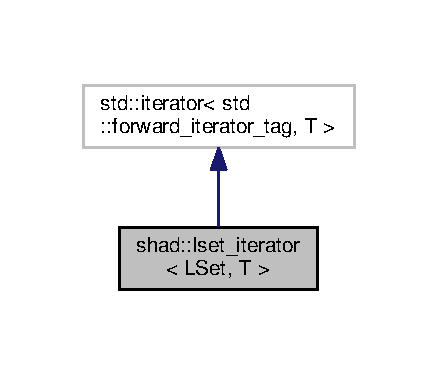
\includegraphics[width=210pt]{classshad_1_1lset__iterator__inherit__graph}
\end{center}
\end{figure}


Collaboration diagram for shad\-:\-:lset\-\_\-iterator$<$ L\-Set, T $>$\-:
\nopagebreak
\begin{figure}[H]
\begin{center}
\leavevmode
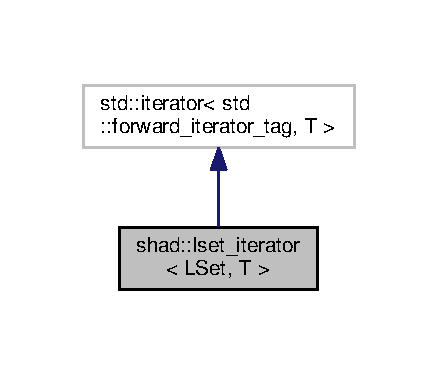
\includegraphics[width=210pt]{classshad_1_1lset__iterator__coll__graph}
\end{center}
\end{figure}
\subsection*{Public Types}
\begin{DoxyCompactItemize}
\item 
using \hyperlink{classshad_1_1lset__iterator_ac9b86123c9a840daa090846707502800}{value\-\_\-type} = T
\item 
using \hyperlink{classshad_1_1lset__iterator_a62e8c31166259f0e57eb48f806f972d0}{Entry} = typename L\-Set\-::\-Entry
\item 
using \hyperlink{classshad_1_1lset__iterator_a15c9f616a8a9f87f058577ec6fb53165}{State} = typename L\-Set\-::\-State
\item 
using \hyperlink{classshad_1_1lset__iterator_a0b81feae1847d0043863c2da36bb87a6}{Bucket} = typename L\-Set\-::\-Bucket
\end{DoxyCompactItemize}
\subsection*{Public Member Functions}
\begin{DoxyCompactItemize}
\item 
\hyperlink{classshad_1_1lset__iterator_a06fb9794dc386f68ad25d623e0651235}{lset\-\_\-iterator} ()
\item 
\hyperlink{classshad_1_1lset__iterator_ac693638bf99a324c15568318028ed490}{lset\-\_\-iterator} (const L\-Set $\ast$set\-Ptr, size\-\_\-t b\-Id, size\-\_\-t pos, \hyperlink{classshad_1_1lset__iterator_a0b81feae1847d0043863c2da36bb87a6}{Bucket} $\ast$cb, \hyperlink{classshad_1_1lset__iterator_a62e8c31166259f0e57eb48f806f972d0}{Entry} $\ast$e\-Ptr)
\item 
bool \hyperlink{classshad_1_1lset__iterator_acb3bbd0bcdc02b25911b195600b674ad}{operator==} (const \hyperlink{classshad_1_1lset__iterator}{lset\-\_\-iterator} \&other) const 
\item 
bool \hyperlink{classshad_1_1lset__iterator_a2bac9439040a4d1fc93b6666c177f210}{operator!=} (const \hyperlink{classshad_1_1lset__iterator}{lset\-\_\-iterator} \&other) const 
\item 
T \hyperlink{classshad_1_1lset__iterator_a05c8551aad5145322484979eecc96c60}{operator$\ast$} () const 
\item 
\hyperlink{classshad_1_1lset__iterator}{lset\-\_\-iterator} \& \hyperlink{classshad_1_1lset__iterator_ab6efcb0bb2f2feeaf0259ebd256aeee5}{operator++} ()
\item 
\hyperlink{classshad_1_1lset__iterator}{lset\-\_\-iterator} \hyperlink{classshad_1_1lset__iterator_a14f424fab2f6dd973555f0dd7d0aa7f8}{operator++} (int)
\end{DoxyCompactItemize}
\subsection*{Static Public Member Functions}
\begin{DoxyCompactItemize}
\item 
static \hyperlink{classshad_1_1lset__iterator}{lset\-\_\-iterator} \hyperlink{classshad_1_1lset__iterator_a388c04d5bf67867300e9cbb0cacbccc4}{lset\-\_\-begin} (const L\-Set $\ast$set\-Ptr)
\item 
static \hyperlink{classshad_1_1lset__iterator}{lset\-\_\-iterator} \hyperlink{classshad_1_1lset__iterator_a4a7319398bbdb69035630c4278f1f07f}{lset\-\_\-end} (const L\-Set $\ast$set\-Ptr)
\item 
static \hyperlink{classshad_1_1lset__iterator}{lset\-\_\-iterator} \hyperlink{classshad_1_1lset__iterator_a1d29fcaa8072432b0f67f9a343e36d95}{lset\-\_\-end} (size\-\_\-t num\-Buckets)
\end{DoxyCompactItemize}
\subsection*{Friends}
\begin{DoxyCompactItemize}
\item 
{\footnotesize template$<$typename , typename , typename $>$ }\\class \hyperlink{classshad_1_1lset__iterator_a51032913d89093f66aa9219f72afe821}{set\-\_\-iterator}
\end{DoxyCompactItemize}


\subsection{Member Typedef Documentation}
\hypertarget{classshad_1_1lset__iterator_a0b81feae1847d0043863c2da36bb87a6}{\index{shad\-::lset\-\_\-iterator@{shad\-::lset\-\_\-iterator}!Bucket@{Bucket}}
\index{Bucket@{Bucket}!shad::lset_iterator@{shad\-::lset\-\_\-iterator}}
\subsubsection[{Bucket}]{\setlength{\rightskip}{0pt plus 5cm}template$<$typename L\-Set , typename T $>$ using {\bf shad\-::lset\-\_\-iterator}$<$ L\-Set, T $>$\-::{\bf Bucket} =  typename L\-Set\-::\-Bucket}}\label{classshad_1_1lset__iterator_a0b81feae1847d0043863c2da36bb87a6}
\hypertarget{classshad_1_1lset__iterator_a62e8c31166259f0e57eb48f806f972d0}{\index{shad\-::lset\-\_\-iterator@{shad\-::lset\-\_\-iterator}!Entry@{Entry}}
\index{Entry@{Entry}!shad::lset_iterator@{shad\-::lset\-\_\-iterator}}
\subsubsection[{Entry}]{\setlength{\rightskip}{0pt plus 5cm}template$<$typename L\-Set , typename T $>$ using {\bf shad\-::lset\-\_\-iterator}$<$ L\-Set, T $>$\-::{\bf Entry} =  typename L\-Set\-::\-Entry}}\label{classshad_1_1lset__iterator_a62e8c31166259f0e57eb48f806f972d0}
\hypertarget{classshad_1_1lset__iterator_a15c9f616a8a9f87f058577ec6fb53165}{\index{shad\-::lset\-\_\-iterator@{shad\-::lset\-\_\-iterator}!State@{State}}
\index{State@{State}!shad::lset_iterator@{shad\-::lset\-\_\-iterator}}
\subsubsection[{State}]{\setlength{\rightskip}{0pt plus 5cm}template$<$typename L\-Set , typename T $>$ using {\bf shad\-::lset\-\_\-iterator}$<$ L\-Set, T $>$\-::{\bf State} =  typename L\-Set\-::\-State}}\label{classshad_1_1lset__iterator_a15c9f616a8a9f87f058577ec6fb53165}
\hypertarget{classshad_1_1lset__iterator_ac9b86123c9a840daa090846707502800}{\index{shad\-::lset\-\_\-iterator@{shad\-::lset\-\_\-iterator}!value\-\_\-type@{value\-\_\-type}}
\index{value\-\_\-type@{value\-\_\-type}!shad::lset_iterator@{shad\-::lset\-\_\-iterator}}
\subsubsection[{value\-\_\-type}]{\setlength{\rightskip}{0pt plus 5cm}template$<$typename L\-Set , typename T $>$ using {\bf shad\-::lset\-\_\-iterator}$<$ L\-Set, T $>$\-::{\bf value\-\_\-type} =  T}}\label{classshad_1_1lset__iterator_ac9b86123c9a840daa090846707502800}


\subsection{Constructor \& Destructor Documentation}
\hypertarget{classshad_1_1lset__iterator_a06fb9794dc386f68ad25d623e0651235}{\index{shad\-::lset\-\_\-iterator@{shad\-::lset\-\_\-iterator}!lset\-\_\-iterator@{lset\-\_\-iterator}}
\index{lset\-\_\-iterator@{lset\-\_\-iterator}!shad::lset_iterator@{shad\-::lset\-\_\-iterator}}
\subsubsection[{lset\-\_\-iterator}]{\setlength{\rightskip}{0pt plus 5cm}template$<$typename L\-Set , typename T $>$ {\bf shad\-::lset\-\_\-iterator}$<$ L\-Set, T $>$\-::{\bf lset\-\_\-iterator} (
\begin{DoxyParamCaption}
{}
\end{DoxyParamCaption}
)\hspace{0.3cm}{\ttfamily [inline]}}}\label{classshad_1_1lset__iterator_a06fb9794dc386f68ad25d623e0651235}
\hypertarget{classshad_1_1lset__iterator_ac693638bf99a324c15568318028ed490}{\index{shad\-::lset\-\_\-iterator@{shad\-::lset\-\_\-iterator}!lset\-\_\-iterator@{lset\-\_\-iterator}}
\index{lset\-\_\-iterator@{lset\-\_\-iterator}!shad::lset_iterator@{shad\-::lset\-\_\-iterator}}
\subsubsection[{lset\-\_\-iterator}]{\setlength{\rightskip}{0pt plus 5cm}template$<$typename L\-Set , typename T $>$ {\bf shad\-::lset\-\_\-iterator}$<$ L\-Set, T $>$\-::{\bf lset\-\_\-iterator} (
\begin{DoxyParamCaption}
\item[{const L\-Set $\ast$}]{set\-Ptr, }
\item[{size\-\_\-t}]{b\-Id, }
\item[{size\-\_\-t}]{pos, }
\item[{{\bf Bucket} $\ast$}]{cb, }
\item[{{\bf Entry} $\ast$}]{e\-Ptr}
\end{DoxyParamCaption}
)\hspace{0.3cm}{\ttfamily [inline]}}}\label{classshad_1_1lset__iterator_ac693638bf99a324c15568318028ed490}


\subsection{Member Function Documentation}
\hypertarget{classshad_1_1lset__iterator_a388c04d5bf67867300e9cbb0cacbccc4}{\index{shad\-::lset\-\_\-iterator@{shad\-::lset\-\_\-iterator}!lset\-\_\-begin@{lset\-\_\-begin}}
\index{lset\-\_\-begin@{lset\-\_\-begin}!shad::lset_iterator@{shad\-::lset\-\_\-iterator}}
\subsubsection[{lset\-\_\-begin}]{\setlength{\rightskip}{0pt plus 5cm}template$<$typename L\-Set , typename T $>$ static {\bf lset\-\_\-iterator} {\bf shad\-::lset\-\_\-iterator}$<$ L\-Set, T $>$\-::lset\-\_\-begin (
\begin{DoxyParamCaption}
\item[{const L\-Set $\ast$}]{set\-Ptr}
\end{DoxyParamCaption}
)\hspace{0.3cm}{\ttfamily [inline]}, {\ttfamily [static]}}}\label{classshad_1_1lset__iterator_a388c04d5bf67867300e9cbb0cacbccc4}
\hypertarget{classshad_1_1lset__iterator_a4a7319398bbdb69035630c4278f1f07f}{\index{shad\-::lset\-\_\-iterator@{shad\-::lset\-\_\-iterator}!lset\-\_\-end@{lset\-\_\-end}}
\index{lset\-\_\-end@{lset\-\_\-end}!shad::lset_iterator@{shad\-::lset\-\_\-iterator}}
\subsubsection[{lset\-\_\-end}]{\setlength{\rightskip}{0pt plus 5cm}template$<$typename L\-Set , typename T $>$ static {\bf lset\-\_\-iterator} {\bf shad\-::lset\-\_\-iterator}$<$ L\-Set, T $>$\-::lset\-\_\-end (
\begin{DoxyParamCaption}
\item[{const L\-Set $\ast$}]{set\-Ptr}
\end{DoxyParamCaption}
)\hspace{0.3cm}{\ttfamily [inline]}, {\ttfamily [static]}}}\label{classshad_1_1lset__iterator_a4a7319398bbdb69035630c4278f1f07f}
\hypertarget{classshad_1_1lset__iterator_a1d29fcaa8072432b0f67f9a343e36d95}{\index{shad\-::lset\-\_\-iterator@{shad\-::lset\-\_\-iterator}!lset\-\_\-end@{lset\-\_\-end}}
\index{lset\-\_\-end@{lset\-\_\-end}!shad::lset_iterator@{shad\-::lset\-\_\-iterator}}
\subsubsection[{lset\-\_\-end}]{\setlength{\rightskip}{0pt plus 5cm}template$<$typename L\-Set , typename T $>$ static {\bf lset\-\_\-iterator} {\bf shad\-::lset\-\_\-iterator}$<$ L\-Set, T $>$\-::lset\-\_\-end (
\begin{DoxyParamCaption}
\item[{size\-\_\-t}]{num\-Buckets}
\end{DoxyParamCaption}
)\hspace{0.3cm}{\ttfamily [inline]}, {\ttfamily [static]}}}\label{classshad_1_1lset__iterator_a1d29fcaa8072432b0f67f9a343e36d95}
\hypertarget{classshad_1_1lset__iterator_a2bac9439040a4d1fc93b6666c177f210}{\index{shad\-::lset\-\_\-iterator@{shad\-::lset\-\_\-iterator}!operator!=@{operator!=}}
\index{operator!=@{operator!=}!shad::lset_iterator@{shad\-::lset\-\_\-iterator}}
\subsubsection[{operator!=}]{\setlength{\rightskip}{0pt plus 5cm}template$<$typename L\-Set , typename T $>$ bool {\bf shad\-::lset\-\_\-iterator}$<$ L\-Set, T $>$\-::operator!= (
\begin{DoxyParamCaption}
\item[{const {\bf lset\-\_\-iterator}$<$ L\-Set, T $>$ \&}]{other}
\end{DoxyParamCaption}
) const\hspace{0.3cm}{\ttfamily [inline]}}}\label{classshad_1_1lset__iterator_a2bac9439040a4d1fc93b6666c177f210}
\hypertarget{classshad_1_1lset__iterator_a05c8551aad5145322484979eecc96c60}{\index{shad\-::lset\-\_\-iterator@{shad\-::lset\-\_\-iterator}!operator$\ast$@{operator$\ast$}}
\index{operator$\ast$@{operator$\ast$}!shad::lset_iterator@{shad\-::lset\-\_\-iterator}}
\subsubsection[{operator$\ast$}]{\setlength{\rightskip}{0pt plus 5cm}template$<$typename L\-Set , typename T $>$ T {\bf shad\-::lset\-\_\-iterator}$<$ L\-Set, T $>$\-::operator$\ast$ (
\begin{DoxyParamCaption}
{}
\end{DoxyParamCaption}
) const\hspace{0.3cm}{\ttfamily [inline]}}}\label{classshad_1_1lset__iterator_a05c8551aad5145322484979eecc96c60}
\hypertarget{classshad_1_1lset__iterator_ab6efcb0bb2f2feeaf0259ebd256aeee5}{\index{shad\-::lset\-\_\-iterator@{shad\-::lset\-\_\-iterator}!operator++@{operator++}}
\index{operator++@{operator++}!shad::lset_iterator@{shad\-::lset\-\_\-iterator}}
\subsubsection[{operator++}]{\setlength{\rightskip}{0pt plus 5cm}template$<$typename L\-Set , typename T $>$ {\bf lset\-\_\-iterator}\& {\bf shad\-::lset\-\_\-iterator}$<$ L\-Set, T $>$\-::operator++ (
\begin{DoxyParamCaption}
{}
\end{DoxyParamCaption}
)\hspace{0.3cm}{\ttfamily [inline]}}}\label{classshad_1_1lset__iterator_ab6efcb0bb2f2feeaf0259ebd256aeee5}
\hypertarget{classshad_1_1lset__iterator_a14f424fab2f6dd973555f0dd7d0aa7f8}{\index{shad\-::lset\-\_\-iterator@{shad\-::lset\-\_\-iterator}!operator++@{operator++}}
\index{operator++@{operator++}!shad::lset_iterator@{shad\-::lset\-\_\-iterator}}
\subsubsection[{operator++}]{\setlength{\rightskip}{0pt plus 5cm}template$<$typename L\-Set , typename T $>$ {\bf lset\-\_\-iterator} {\bf shad\-::lset\-\_\-iterator}$<$ L\-Set, T $>$\-::operator++ (
\begin{DoxyParamCaption}
\item[{int}]{}
\end{DoxyParamCaption}
)\hspace{0.3cm}{\ttfamily [inline]}}}\label{classshad_1_1lset__iterator_a14f424fab2f6dd973555f0dd7d0aa7f8}
\hypertarget{classshad_1_1lset__iterator_acb3bbd0bcdc02b25911b195600b674ad}{\index{shad\-::lset\-\_\-iterator@{shad\-::lset\-\_\-iterator}!operator==@{operator==}}
\index{operator==@{operator==}!shad::lset_iterator@{shad\-::lset\-\_\-iterator}}
\subsubsection[{operator==}]{\setlength{\rightskip}{0pt plus 5cm}template$<$typename L\-Set , typename T $>$ bool {\bf shad\-::lset\-\_\-iterator}$<$ L\-Set, T $>$\-::operator== (
\begin{DoxyParamCaption}
\item[{const {\bf lset\-\_\-iterator}$<$ L\-Set, T $>$ \&}]{other}
\end{DoxyParamCaption}
) const\hspace{0.3cm}{\ttfamily [inline]}}}\label{classshad_1_1lset__iterator_acb3bbd0bcdc02b25911b195600b674ad}


\subsection{Friends And Related Function Documentation}
\hypertarget{classshad_1_1lset__iterator_a51032913d89093f66aa9219f72afe821}{\index{shad\-::lset\-\_\-iterator@{shad\-::lset\-\_\-iterator}!set\-\_\-iterator@{set\-\_\-iterator}}
\index{set\-\_\-iterator@{set\-\_\-iterator}!shad::lset_iterator@{shad\-::lset\-\_\-iterator}}
\subsubsection[{set\-\_\-iterator}]{\setlength{\rightskip}{0pt plus 5cm}template$<$typename L\-Set , typename T $>$ template$<$typename , typename , typename $>$ friend class {\bf set\-\_\-iterator}\hspace{0.3cm}{\ttfamily [friend]}}}\label{classshad_1_1lset__iterator_a51032913d89093f66aa9219f72afe821}


The documentation for this class was generated from the following file\-:\begin{DoxyCompactItemize}
\item 
include/shad/data\-\_\-structures/\hyperlink{local__set_8h}{local\-\_\-set.\-h}\end{DoxyCompactItemize}

\hypertarget{classshad_1_1map__iterator}{\section{shad\-:\-:map\-\_\-iterator$<$ Map, T, Non\-Const\-T $>$ Class Template Reference}
\label{classshad_1_1map__iterator}\index{shad\-::map\-\_\-iterator$<$ Map, T, Non\-Const\-T $>$@{shad\-::map\-\_\-iterator$<$ Map, T, Non\-Const\-T $>$}}
}


{\ttfamily \#include $<$shad/data\-\_\-structures/hashmap.\-h$>$}



Inheritance diagram for shad\-:\-:map\-\_\-iterator$<$ Map, T, Non\-Const\-T $>$\-:
\nopagebreak
\begin{figure}[H]
\begin{center}
\leavevmode
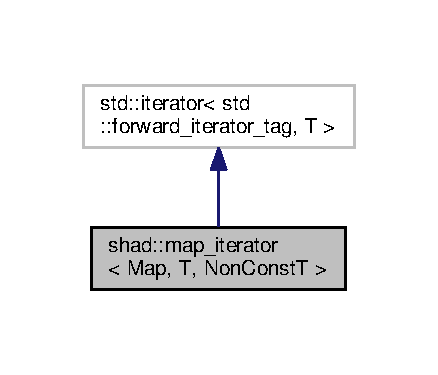
\includegraphics[width=210pt]{classshad_1_1map__iterator__inherit__graph}
\end{center}
\end{figure}


Collaboration diagram for shad\-:\-:map\-\_\-iterator$<$ Map, T, Non\-Const\-T $>$\-:
\nopagebreak
\begin{figure}[H]
\begin{center}
\leavevmode
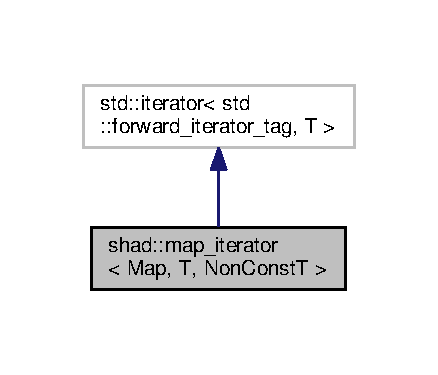
\includegraphics[width=210pt]{classshad_1_1map__iterator__coll__graph}
\end{center}
\end{figure}
\subsection*{Classes}
\begin{DoxyCompactItemize}
\item 
class \hyperlink{classshad_1_1map__iterator_1_1local__iterator__range}{local\-\_\-iterator\-\_\-range}
\end{DoxyCompactItemize}
\subsection*{Public Types}
\begin{DoxyCompactItemize}
\item 
using \hyperlink{classshad_1_1map__iterator_aecdaced930b9dcb48d5eff9ef992fbd5}{O\-I\-D\-T} = typename Map\-T\-::\-Object\-I\-D
\item 
using \hyperlink{classshad_1_1map__iterator_a157d8b69a2befd7e61c0df9eb52b2a71}{L\-Map} = typename Map\-T\-::\-L\-Map\-T
\item 
using \hyperlink{classshad_1_1map__iterator_adceb72a3948aa860edd3a4c9ceca821d}{local\-\_\-iterator\-\_\-type} = \hyperlink{classshad_1_1lmap__iterator}{lmap\-\_\-iterator}$<$ \hyperlink{classshad_1_1map__iterator_a157d8b69a2befd7e61c0df9eb52b2a71}{L\-Map}, T $>$
\item 
using \hyperlink{classshad_1_1map__iterator_a52d94a1de8e6027b63d1a72daf0ff3d0}{value\-\_\-type} = T
\end{DoxyCompactItemize}
\subsection*{Public Member Functions}
\begin{DoxyCompactItemize}
\item 
\hyperlink{classshad_1_1map__iterator_a085dcb1354b6b6b7326c69efd3c228e6}{map\-\_\-iterator} ()
\item 
\hyperlink{classshad_1_1map__iterator_ac93f17a66ee8c0569d5700134b263f39}{map\-\_\-iterator} (uint32\-\_\-t loc\-I\-D, const \hyperlink{classshad_1_1map__iterator_aecdaced930b9dcb48d5eff9ef992fbd5}{O\-I\-D\-T} map\-O\-I\-D, \hyperlink{classshad_1_1map__iterator_adceb72a3948aa860edd3a4c9ceca821d}{local\-\_\-iterator\-\_\-type} \&lit, T element)
\item 
\hyperlink{classshad_1_1map__iterator_aac7de0f8d21acd08be67f02aec45f3d3}{map\-\_\-iterator} (uint32\-\_\-t loc\-I\-D, const \hyperlink{classshad_1_1map__iterator_aecdaced930b9dcb48d5eff9ef992fbd5}{O\-I\-D\-T} map\-O\-I\-D, \hyperlink{classshad_1_1map__iterator_adceb72a3948aa860edd3a4c9ceca821d}{local\-\_\-iterator\-\_\-type} \&lit)
\item 
bool \hyperlink{classshad_1_1map__iterator_a84b9e374f5420dbf1c3c6e22e7a0958f}{operator==} (const \hyperlink{classshad_1_1map__iterator}{map\-\_\-iterator} \&other) const 
\item 
bool \hyperlink{classshad_1_1map__iterator_af3bf9fb8d3abca27b66e7cfd192e34cd}{operator!=} (const \hyperlink{classshad_1_1map__iterator}{map\-\_\-iterator} \&other) const 
\item 
T \hyperlink{classshad_1_1map__iterator_a783e686ed5416838221177430bf136ce}{operator$\ast$} () const 
\item 
\hyperlink{classshad_1_1map__iterator}{map\-\_\-iterator} \& \hyperlink{classshad_1_1map__iterator_ad8d506efca132c4219e7e011230387b5}{operator++} ()
\item 
\hyperlink{classshad_1_1map__iterator}{map\-\_\-iterator} \hyperlink{classshad_1_1map__iterator_af899decfb38395fc586a6eb4bfe8f8f9}{operator++} (int)
\end{DoxyCompactItemize}
\subsection*{Static Public Member Functions}
\begin{DoxyCompactItemize}
\item 
static \hyperlink{classshad_1_1map__iterator}{map\-\_\-iterator} \hyperlink{classshad_1_1map__iterator_a57d139353cfaa75639f6445a0e138c7d}{map\-\_\-begin} (const Map\-T $\ast$map\-Ptr)
\item 
static \hyperlink{classshad_1_1map__iterator}{map\-\_\-iterator} \hyperlink{classshad_1_1map__iterator_a3f9cd178ba9a8d529844cf215be6a79b}{map\-\_\-end} (const Map\-T $\ast$map\-Ptr)
\item 
static \hyperlink{classshad_1_1map__iterator_1_1local__iterator__range}{local\-\_\-iterator\-\_\-range} \hyperlink{classshad_1_1map__iterator_aae44fbc7ffd3ceb7cb80a8661cb74c34}{local\-\_\-range} (\hyperlink{classshad_1_1map__iterator}{map\-\_\-iterator} \&B, \hyperlink{classshad_1_1map__iterator}{map\-\_\-iterator} \&E)
\item 
static \hyperlink{classshad_1_1rt_1_1localities__range}{rt\-::localities\-\_\-range} \hyperlink{classshad_1_1map__iterator_ae809bb004b5f198eae11dfe7ac9c5f8a}{localities} (\hyperlink{classshad_1_1map__iterator}{map\-\_\-iterator} \&B, \hyperlink{classshad_1_1map__iterator}{map\-\_\-iterator} \&E)
\item 
static \hyperlink{classshad_1_1map__iterator}{map\-\_\-iterator} \hyperlink{classshad_1_1map__iterator_af5d464e76c35e666c792bb948f5d6739}{iterator\-\_\-from\-\_\-local} (\hyperlink{classshad_1_1map__iterator}{map\-\_\-iterator} \&B, \hyperlink{classshad_1_1map__iterator}{map\-\_\-iterator} \&E, \hyperlink{classshad_1_1map__iterator_adceb72a3948aa860edd3a4c9ceca821d}{local\-\_\-iterator\-\_\-type} itr)
\end{DoxyCompactItemize}


\subsection{Member Typedef Documentation}
\hypertarget{classshad_1_1map__iterator_a157d8b69a2befd7e61c0df9eb52b2a71}{\index{shad\-::map\-\_\-iterator@{shad\-::map\-\_\-iterator}!L\-Map@{L\-Map}}
\index{L\-Map@{L\-Map}!shad::map_iterator@{shad\-::map\-\_\-iterator}}
\subsubsection[{L\-Map}]{\setlength{\rightskip}{0pt plus 5cm}template$<$typename Map , typename T , typename Non\-Const\-T $>$ using {\bf shad\-::map\-\_\-iterator}$<$ Map, T, Non\-Const\-T $>$\-::{\bf L\-Map} =  typename Map\-T\-::\-L\-Map\-T}}\label{classshad_1_1map__iterator_a157d8b69a2befd7e61c0df9eb52b2a71}
\hypertarget{classshad_1_1map__iterator_adceb72a3948aa860edd3a4c9ceca821d}{\index{shad\-::map\-\_\-iterator@{shad\-::map\-\_\-iterator}!local\-\_\-iterator\-\_\-type@{local\-\_\-iterator\-\_\-type}}
\index{local\-\_\-iterator\-\_\-type@{local\-\_\-iterator\-\_\-type}!shad::map_iterator@{shad\-::map\-\_\-iterator}}
\subsubsection[{local\-\_\-iterator\-\_\-type}]{\setlength{\rightskip}{0pt plus 5cm}template$<$typename Map , typename T , typename Non\-Const\-T $>$ using {\bf shad\-::map\-\_\-iterator}$<$ Map, T, Non\-Const\-T $>$\-::{\bf local\-\_\-iterator\-\_\-type} =  {\bf lmap\-\_\-iterator}$<${\bf L\-Map}, T$>$}}\label{classshad_1_1map__iterator_adceb72a3948aa860edd3a4c9ceca821d}
\hypertarget{classshad_1_1map__iterator_aecdaced930b9dcb48d5eff9ef992fbd5}{\index{shad\-::map\-\_\-iterator@{shad\-::map\-\_\-iterator}!O\-I\-D\-T@{O\-I\-D\-T}}
\index{O\-I\-D\-T@{O\-I\-D\-T}!shad::map_iterator@{shad\-::map\-\_\-iterator}}
\subsubsection[{O\-I\-D\-T}]{\setlength{\rightskip}{0pt plus 5cm}template$<$typename Map , typename T , typename Non\-Const\-T $>$ using {\bf shad\-::map\-\_\-iterator}$<$ Map, T, Non\-Const\-T $>$\-::{\bf O\-I\-D\-T} =  typename Map\-T\-::\-Object\-I\-D}}\label{classshad_1_1map__iterator_aecdaced930b9dcb48d5eff9ef992fbd5}
\hypertarget{classshad_1_1map__iterator_a52d94a1de8e6027b63d1a72daf0ff3d0}{\index{shad\-::map\-\_\-iterator@{shad\-::map\-\_\-iterator}!value\-\_\-type@{value\-\_\-type}}
\index{value\-\_\-type@{value\-\_\-type}!shad::map_iterator@{shad\-::map\-\_\-iterator}}
\subsubsection[{value\-\_\-type}]{\setlength{\rightskip}{0pt plus 5cm}template$<$typename Map , typename T , typename Non\-Const\-T $>$ using {\bf shad\-::map\-\_\-iterator}$<$ Map, T, Non\-Const\-T $>$\-::{\bf value\-\_\-type} =  T}}\label{classshad_1_1map__iterator_a52d94a1de8e6027b63d1a72daf0ff3d0}


\subsection{Constructor \& Destructor Documentation}
\hypertarget{classshad_1_1map__iterator_a085dcb1354b6b6b7326c69efd3c228e6}{\index{shad\-::map\-\_\-iterator@{shad\-::map\-\_\-iterator}!map\-\_\-iterator@{map\-\_\-iterator}}
\index{map\-\_\-iterator@{map\-\_\-iterator}!shad::map_iterator@{shad\-::map\-\_\-iterator}}
\subsubsection[{map\-\_\-iterator}]{\setlength{\rightskip}{0pt plus 5cm}template$<$typename Map , typename T , typename Non\-Const\-T $>$ {\bf shad\-::map\-\_\-iterator}$<$ Map, T, Non\-Const\-T $>$\-::{\bf map\-\_\-iterator} (
\begin{DoxyParamCaption}
{}
\end{DoxyParamCaption}
)\hspace{0.3cm}{\ttfamily [inline]}}}\label{classshad_1_1map__iterator_a085dcb1354b6b6b7326c69efd3c228e6}
\hypertarget{classshad_1_1map__iterator_ac93f17a66ee8c0569d5700134b263f39}{\index{shad\-::map\-\_\-iterator@{shad\-::map\-\_\-iterator}!map\-\_\-iterator@{map\-\_\-iterator}}
\index{map\-\_\-iterator@{map\-\_\-iterator}!shad::map_iterator@{shad\-::map\-\_\-iterator}}
\subsubsection[{map\-\_\-iterator}]{\setlength{\rightskip}{0pt plus 5cm}template$<$typename Map , typename T , typename Non\-Const\-T $>$ {\bf shad\-::map\-\_\-iterator}$<$ Map, T, Non\-Const\-T $>$\-::{\bf map\-\_\-iterator} (
\begin{DoxyParamCaption}
\item[{uint32\-\_\-t}]{loc\-I\-D, }
\item[{const {\bf O\-I\-D\-T}}]{map\-O\-I\-D, }
\item[{{\bf local\-\_\-iterator\-\_\-type} \&}]{lit, }
\item[{T}]{element}
\end{DoxyParamCaption}
)\hspace{0.3cm}{\ttfamily [inline]}}}\label{classshad_1_1map__iterator_ac93f17a66ee8c0569d5700134b263f39}
\hypertarget{classshad_1_1map__iterator_aac7de0f8d21acd08be67f02aec45f3d3}{\index{shad\-::map\-\_\-iterator@{shad\-::map\-\_\-iterator}!map\-\_\-iterator@{map\-\_\-iterator}}
\index{map\-\_\-iterator@{map\-\_\-iterator}!shad::map_iterator@{shad\-::map\-\_\-iterator}}
\subsubsection[{map\-\_\-iterator}]{\setlength{\rightskip}{0pt plus 5cm}template$<$typename Map , typename T , typename Non\-Const\-T $>$ {\bf shad\-::map\-\_\-iterator}$<$ Map, T, Non\-Const\-T $>$\-::{\bf map\-\_\-iterator} (
\begin{DoxyParamCaption}
\item[{uint32\-\_\-t}]{loc\-I\-D, }
\item[{const {\bf O\-I\-D\-T}}]{map\-O\-I\-D, }
\item[{{\bf local\-\_\-iterator\-\_\-type} \&}]{lit}
\end{DoxyParamCaption}
)\hspace{0.3cm}{\ttfamily [inline]}}}\label{classshad_1_1map__iterator_aac7de0f8d21acd08be67f02aec45f3d3}


\subsection{Member Function Documentation}
\hypertarget{classshad_1_1map__iterator_af5d464e76c35e666c792bb948f5d6739}{\index{shad\-::map\-\_\-iterator@{shad\-::map\-\_\-iterator}!iterator\-\_\-from\-\_\-local@{iterator\-\_\-from\-\_\-local}}
\index{iterator\-\_\-from\-\_\-local@{iterator\-\_\-from\-\_\-local}!shad::map_iterator@{shad\-::map\-\_\-iterator}}
\subsubsection[{iterator\-\_\-from\-\_\-local}]{\setlength{\rightskip}{0pt plus 5cm}template$<$typename Map , typename T , typename Non\-Const\-T $>$ static {\bf map\-\_\-iterator} {\bf shad\-::map\-\_\-iterator}$<$ Map, T, Non\-Const\-T $>$\-::iterator\-\_\-from\-\_\-local (
\begin{DoxyParamCaption}
\item[{{\bf map\-\_\-iterator}$<$ Map, T, Non\-Const\-T $>$ \&}]{B, }
\item[{{\bf map\-\_\-iterator}$<$ Map, T, Non\-Const\-T $>$ \&}]{E, }
\item[{{\bf local\-\_\-iterator\-\_\-type}}]{itr}
\end{DoxyParamCaption}
)\hspace{0.3cm}{\ttfamily [inline]}, {\ttfamily [static]}}}\label{classshad_1_1map__iterator_af5d464e76c35e666c792bb948f5d6739}
\hypertarget{classshad_1_1map__iterator_aae44fbc7ffd3ceb7cb80a8661cb74c34}{\index{shad\-::map\-\_\-iterator@{shad\-::map\-\_\-iterator}!local\-\_\-range@{local\-\_\-range}}
\index{local\-\_\-range@{local\-\_\-range}!shad::map_iterator@{shad\-::map\-\_\-iterator}}
\subsubsection[{local\-\_\-range}]{\setlength{\rightskip}{0pt plus 5cm}template$<$typename Map , typename T , typename Non\-Const\-T $>$ static {\bf local\-\_\-iterator\-\_\-range} {\bf shad\-::map\-\_\-iterator}$<$ Map, T, Non\-Const\-T $>$\-::local\-\_\-range (
\begin{DoxyParamCaption}
\item[{{\bf map\-\_\-iterator}$<$ Map, T, Non\-Const\-T $>$ \&}]{B, }
\item[{{\bf map\-\_\-iterator}$<$ Map, T, Non\-Const\-T $>$ \&}]{E}
\end{DoxyParamCaption}
)\hspace{0.3cm}{\ttfamily [inline]}, {\ttfamily [static]}}}\label{classshad_1_1map__iterator_aae44fbc7ffd3ceb7cb80a8661cb74c34}
\hypertarget{classshad_1_1map__iterator_ae809bb004b5f198eae11dfe7ac9c5f8a}{\index{shad\-::map\-\_\-iterator@{shad\-::map\-\_\-iterator}!localities@{localities}}
\index{localities@{localities}!shad::map_iterator@{shad\-::map\-\_\-iterator}}
\subsubsection[{localities}]{\setlength{\rightskip}{0pt plus 5cm}template$<$typename Map , typename T , typename Non\-Const\-T $>$ static {\bf rt\-::localities\-\_\-range} {\bf shad\-::map\-\_\-iterator}$<$ Map, T, Non\-Const\-T $>$\-::localities (
\begin{DoxyParamCaption}
\item[{{\bf map\-\_\-iterator}$<$ Map, T, Non\-Const\-T $>$ \&}]{B, }
\item[{{\bf map\-\_\-iterator}$<$ Map, T, Non\-Const\-T $>$ \&}]{E}
\end{DoxyParamCaption}
)\hspace{0.3cm}{\ttfamily [inline]}, {\ttfamily [static]}}}\label{classshad_1_1map__iterator_ae809bb004b5f198eae11dfe7ac9c5f8a}
\hypertarget{classshad_1_1map__iterator_a57d139353cfaa75639f6445a0e138c7d}{\index{shad\-::map\-\_\-iterator@{shad\-::map\-\_\-iterator}!map\-\_\-begin@{map\-\_\-begin}}
\index{map\-\_\-begin@{map\-\_\-begin}!shad::map_iterator@{shad\-::map\-\_\-iterator}}
\subsubsection[{map\-\_\-begin}]{\setlength{\rightskip}{0pt plus 5cm}template$<$typename Map , typename T , typename Non\-Const\-T $>$ static {\bf map\-\_\-iterator} {\bf shad\-::map\-\_\-iterator}$<$ Map, T, Non\-Const\-T $>$\-::map\-\_\-begin (
\begin{DoxyParamCaption}
\item[{const Map\-T $\ast$}]{map\-Ptr}
\end{DoxyParamCaption}
)\hspace{0.3cm}{\ttfamily [inline]}, {\ttfamily [static]}}}\label{classshad_1_1map__iterator_a57d139353cfaa75639f6445a0e138c7d}
\hypertarget{classshad_1_1map__iterator_a3f9cd178ba9a8d529844cf215be6a79b}{\index{shad\-::map\-\_\-iterator@{shad\-::map\-\_\-iterator}!map\-\_\-end@{map\-\_\-end}}
\index{map\-\_\-end@{map\-\_\-end}!shad::map_iterator@{shad\-::map\-\_\-iterator}}
\subsubsection[{map\-\_\-end}]{\setlength{\rightskip}{0pt plus 5cm}template$<$typename Map , typename T , typename Non\-Const\-T $>$ static {\bf map\-\_\-iterator} {\bf shad\-::map\-\_\-iterator}$<$ Map, T, Non\-Const\-T $>$\-::map\-\_\-end (
\begin{DoxyParamCaption}
\item[{const Map\-T $\ast$}]{map\-Ptr}
\end{DoxyParamCaption}
)\hspace{0.3cm}{\ttfamily [inline]}, {\ttfamily [static]}}}\label{classshad_1_1map__iterator_a3f9cd178ba9a8d529844cf215be6a79b}
\hypertarget{classshad_1_1map__iterator_af3bf9fb8d3abca27b66e7cfd192e34cd}{\index{shad\-::map\-\_\-iterator@{shad\-::map\-\_\-iterator}!operator!=@{operator!=}}
\index{operator!=@{operator!=}!shad::map_iterator@{shad\-::map\-\_\-iterator}}
\subsubsection[{operator!=}]{\setlength{\rightskip}{0pt plus 5cm}template$<$typename Map , typename T , typename Non\-Const\-T $>$ bool {\bf shad\-::map\-\_\-iterator}$<$ Map, T, Non\-Const\-T $>$\-::operator!= (
\begin{DoxyParamCaption}
\item[{const {\bf map\-\_\-iterator}$<$ Map, T, Non\-Const\-T $>$ \&}]{other}
\end{DoxyParamCaption}
) const\hspace{0.3cm}{\ttfamily [inline]}}}\label{classshad_1_1map__iterator_af3bf9fb8d3abca27b66e7cfd192e34cd}
\hypertarget{classshad_1_1map__iterator_a783e686ed5416838221177430bf136ce}{\index{shad\-::map\-\_\-iterator@{shad\-::map\-\_\-iterator}!operator$\ast$@{operator$\ast$}}
\index{operator$\ast$@{operator$\ast$}!shad::map_iterator@{shad\-::map\-\_\-iterator}}
\subsubsection[{operator$\ast$}]{\setlength{\rightskip}{0pt plus 5cm}template$<$typename Map , typename T , typename Non\-Const\-T $>$ T {\bf shad\-::map\-\_\-iterator}$<$ Map, T, Non\-Const\-T $>$\-::operator$\ast$ (
\begin{DoxyParamCaption}
{}
\end{DoxyParamCaption}
) const\hspace{0.3cm}{\ttfamily [inline]}}}\label{classshad_1_1map__iterator_a783e686ed5416838221177430bf136ce}
\hypertarget{classshad_1_1map__iterator_ad8d506efca132c4219e7e011230387b5}{\index{shad\-::map\-\_\-iterator@{shad\-::map\-\_\-iterator}!operator++@{operator++}}
\index{operator++@{operator++}!shad::map_iterator@{shad\-::map\-\_\-iterator}}
\subsubsection[{operator++}]{\setlength{\rightskip}{0pt plus 5cm}template$<$typename Map , typename T , typename Non\-Const\-T $>$ {\bf map\-\_\-iterator}\& {\bf shad\-::map\-\_\-iterator}$<$ Map, T, Non\-Const\-T $>$\-::operator++ (
\begin{DoxyParamCaption}
{}
\end{DoxyParamCaption}
)\hspace{0.3cm}{\ttfamily [inline]}}}\label{classshad_1_1map__iterator_ad8d506efca132c4219e7e011230387b5}
\hypertarget{classshad_1_1map__iterator_af899decfb38395fc586a6eb4bfe8f8f9}{\index{shad\-::map\-\_\-iterator@{shad\-::map\-\_\-iterator}!operator++@{operator++}}
\index{operator++@{operator++}!shad::map_iterator@{shad\-::map\-\_\-iterator}}
\subsubsection[{operator++}]{\setlength{\rightskip}{0pt plus 5cm}template$<$typename Map , typename T , typename Non\-Const\-T $>$ {\bf map\-\_\-iterator} {\bf shad\-::map\-\_\-iterator}$<$ Map, T, Non\-Const\-T $>$\-::operator++ (
\begin{DoxyParamCaption}
\item[{int}]{}
\end{DoxyParamCaption}
)\hspace{0.3cm}{\ttfamily [inline]}}}\label{classshad_1_1map__iterator_af899decfb38395fc586a6eb4bfe8f8f9}
\hypertarget{classshad_1_1map__iterator_a84b9e374f5420dbf1c3c6e22e7a0958f}{\index{shad\-::map\-\_\-iterator@{shad\-::map\-\_\-iterator}!operator==@{operator==}}
\index{operator==@{operator==}!shad::map_iterator@{shad\-::map\-\_\-iterator}}
\subsubsection[{operator==}]{\setlength{\rightskip}{0pt plus 5cm}template$<$typename Map , typename T , typename Non\-Const\-T $>$ bool {\bf shad\-::map\-\_\-iterator}$<$ Map, T, Non\-Const\-T $>$\-::operator== (
\begin{DoxyParamCaption}
\item[{const {\bf map\-\_\-iterator}$<$ Map, T, Non\-Const\-T $>$ \&}]{other}
\end{DoxyParamCaption}
) const\hspace{0.3cm}{\ttfamily [inline]}}}\label{classshad_1_1map__iterator_a84b9e374f5420dbf1c3c6e22e7a0958f}


The documentation for this class was generated from the following file\-:\begin{DoxyCompactItemize}
\item 
include/shad/data\-\_\-structures/\hyperlink{hashmap_8h}{hashmap.\-h}\end{DoxyCompactItemize}

\hypertarget{structshad_1_1measure}{\section{shad\-:\-:measure$<$ Time\-T $>$ Struct Template Reference}
\label{structshad_1_1measure}\index{shad\-::measure$<$ Time\-T $>$@{shad\-::measure$<$ Time\-T $>$}}
}


Utility for time measurements.  




{\ttfamily \#include $<$shad/util/measure.\-h$>$}

\subsection*{Static Public Member Functions}
\begin{DoxyCompactItemize}
\item 
{\footnotesize template$<$typename F , typename... Args$>$ }\\static auto \hyperlink{structshad_1_1measure_a2860ac23e7be931cabad22763ef03602}{duration} (F \&\&function, Args...\-args)
\begin{DoxyCompactList}\small\item\em Compute the time spend to execute a function. \end{DoxyCompactList}\end{DoxyCompactItemize}


\subsection{Detailed Description}
\subsubsection*{template$<$typename Time\-T = std\-::chrono\-::milliseconds$>$struct shad\-::measure$<$ Time\-T $>$}

Utility for time measurements. 

\subsection{Member Function Documentation}
\hypertarget{structshad_1_1measure_a2860ac23e7be931cabad22763ef03602}{\index{shad\-::measure@{shad\-::measure}!duration@{duration}}
\index{duration@{duration}!shad::measure@{shad\-::measure}}
\subsubsection[{duration}]{\setlength{\rightskip}{0pt plus 5cm}template$<$typename Time\-T  = std\-::chrono\-::milliseconds$>$ template$<$typename F , typename... Args$>$ static auto {\bf shad\-::measure}$<$ Time\-T $>$\-::duration (
\begin{DoxyParamCaption}
\item[{F \&\&}]{function, }
\item[{Args...}]{args}
\end{DoxyParamCaption}
)\hspace{0.3cm}{\ttfamily [inline]}, {\ttfamily [static]}}}\label{structshad_1_1measure_a2860ac23e7be931cabad22763ef03602}


Compute the time spend to execute a function. 

Typical Usage\-: 
\begin{DoxyCode}
\textcolor{keywordtype}{int} aParameter = 1;
\textcolor{keyword}{auto} time = \hyperlink{structshad_1_1measure_a2860ac23e7be931cabad22763ef03602}{shad::measure<std::chrono::seconds>::duration}(
  [](\textcolor{keywordtype}{int} aParameter) \{
    \textcolor{comment}{// ... do what needs to be measured ...}
  \}, aParameter);

std::cout << \textcolor{stringliteral}{"Time spent : "} << time.count() << std::endl;
\end{DoxyCode}



\begin{DoxyTemplParams}{Template Parameters}
{\em F} & The type of the function to be computed \\
\hline
{\em Args} & The types of the arguments to be forwarded to the function.\\
\hline
\end{DoxyTemplParams}

\begin{DoxyParams}[1]{Parameters}
\mbox{\tt in}  & {\em function} & A collable object that will be measured \\
\hline
\mbox{\tt in}  & {\em args} & The list of args forwarded to the function. \\
\hline
\end{DoxyParams}
\begin{DoxyReturn}{Returns}
the time spent to compute the input function. 
\end{DoxyReturn}


The documentation for this struct was generated from the following file\-:\begin{DoxyCompactItemize}
\item 
include/shad/util/\hyperlink{measure_8h}{measure.\-h}\end{DoxyCompactItemize}

\hypertarget{classshad_1_1MemCmp}{\section{shad\-:\-:Mem\-Cmp$<$ Key\-Ty $>$ Class Template Reference}
\label{classshad_1_1MemCmp}\index{shad\-::\-Mem\-Cmp$<$ Key\-Ty $>$@{shad\-::\-Mem\-Cmp$<$ Key\-Ty $>$}}
}


Comparison functor.  




{\ttfamily \#include $<$shad/data\-\_\-structures/compare\-\_\-and\-\_\-hash\-\_\-utils.\-h$>$}

\subsection*{Public Member Functions}
\begin{DoxyCompactItemize}
\item 
bool \hyperlink{classshad_1_1MemCmp_aab48de1966a6e2056bcb9aa6232707b0}{operator()} (const Key\-Ty $\ast$first, const Key\-Ty $\ast$second) const 
\end{DoxyCompactItemize}


\subsection{Detailed Description}
\subsubsection*{template$<$typename Key\-Ty$>$class shad\-::\-Mem\-Cmp$<$ Key\-Ty $>$}

Comparison functor. 

This functor compares two object of type Key\-Ty.

Typical Usage\-: 
\begin{DoxyCode}
\textcolor{keyword}{struct }A \{
  \textcolor{keywordtype}{int} a, b;
\};

\textcolor{keywordtype}{void} fn(A value1, A value2) \{
  \textcolor{keywordflow}{if} (!MemCmp()(&value1, &value2)) \{
    \textcolor{comment}{// they are equal so do something}
  \} \textcolor{keywordflow}{else} \{
    \textcolor{comment}{// do sothing different}
  \}
\}
\end{DoxyCode}



\begin{DoxyTemplParams}{Template Parameters}
{\em Key\-Ty} & The type of the two keys to compare.\\
\hline
\end{DoxyTemplParams}

\begin{DoxyParams}[1]{Parameters}
\mbox{\tt in}  & {\em first} & The first object to be compared \\
\hline
\mbox{\tt in}  & {\em second} & The second object to be compared \\
\hline
\end{DoxyParams}
\begin{DoxyReturn}{Returns}
false if first == second, true otherwise. 
\end{DoxyReturn}


\subsection{Member Function Documentation}
\hypertarget{classshad_1_1MemCmp_aab48de1966a6e2056bcb9aa6232707b0}{\index{shad\-::\-Mem\-Cmp@{shad\-::\-Mem\-Cmp}!operator()@{operator()}}
\index{operator()@{operator()}!shad::MemCmp@{shad\-::\-Mem\-Cmp}}
\subsubsection[{operator()}]{\setlength{\rightskip}{0pt plus 5cm}template$<$typename Key\-Ty$>$ bool {\bf shad\-::\-Mem\-Cmp}$<$ Key\-Ty $>$\-::operator() (
\begin{DoxyParamCaption}
\item[{const Key\-Ty $\ast$}]{first, }
\item[{const Key\-Ty $\ast$}]{second}
\end{DoxyParamCaption}
) const\hspace{0.3cm}{\ttfamily [inline]}}}\label{classshad_1_1MemCmp_aab48de1966a6e2056bcb9aa6232707b0}


The documentation for this class was generated from the following file\-:\begin{DoxyCompactItemize}
\item 
include/shad/data\-\_\-structures/\hyperlink{compare__and__hash__utils_8h}{compare\-\_\-and\-\_\-hash\-\_\-utils.\-h}\end{DoxyCompactItemize}

\hypertarget{classshad_1_1MemCmp_3_01std_1_1vector_3_01KeyTy_01_4_01_4}{\section{shad\-:\-:Mem\-Cmp$<$ std\-:\-:vector$<$ Key\-Ty $>$ $>$ Class Template Reference}
\label{classshad_1_1MemCmp_3_01std_1_1vector_3_01KeyTy_01_4_01_4}\index{shad\-::\-Mem\-Cmp$<$ std\-::vector$<$ Key\-Ty $>$ $>$@{shad\-::\-Mem\-Cmp$<$ std\-::vector$<$ Key\-Ty $>$ $>$}}
}


Comparison functor specialized for std\-::vector.  




{\ttfamily \#include $<$shad/data\-\_\-structures/compare\-\_\-and\-\_\-hash\-\_\-utils.\-h$>$}

\subsection*{Public Member Functions}
\begin{DoxyCompactItemize}
\item 
bool \hyperlink{classshad_1_1MemCmp_3_01std_1_1vector_3_01KeyTy_01_4_01_4_aeacb3178b19255d7c248f46bda51a7bd}{operator()} (const std\-::vector$<$ Key\-Ty $>$ $\ast$first, const std\-::vector$<$ Key\-Ty $>$ $\ast$sec) const 
\end{DoxyCompactItemize}


\subsection{Detailed Description}
\subsubsection*{template$<$typename Key\-Ty$>$class shad\-::\-Mem\-Cmp$<$ std\-::vector$<$ Key\-Ty $>$ $>$}

Comparison functor specialized for std\-::vector. 

This functor compares the content of two std\-::vector.

Typical Usage\-: 
\begin{DoxyCode}
\textcolor{keyword}{struct }A \{
  \textcolor{keywordtype}{int} a, b;
\};

\textcolor{keywordtype}{void} fn(std::vector<A> &value1, std::vector<A> & value2) \{
  \textcolor{keywordflow}{if} (!MemCmp()(&value1, &value2)) \{
    \textcolor{comment}{// they are equal so do something}
  \} \textcolor{keywordflow}{else} \{
    \textcolor{comment}{// do sothing different}
  \}
\}
\end{DoxyCode}



\begin{DoxyTemplParams}{Template Parameters}
{\em Key\-Ty} & The type of the two keys to compare.\\
\hline
\end{DoxyTemplParams}

\begin{DoxyParams}[1]{Parameters}
\mbox{\tt in}  & {\em first} & The first std\-::vector to be compared \\
\hline
\mbox{\tt in}  & {\em second} & The second std\-::vector to be compared \\
\hline
\end{DoxyParams}
\begin{DoxyReturn}{Returns}
false if first == second, true otherwise. 
\end{DoxyReturn}


\subsection{Member Function Documentation}
\hypertarget{classshad_1_1MemCmp_3_01std_1_1vector_3_01KeyTy_01_4_01_4_aeacb3178b19255d7c248f46bda51a7bd}{\index{shad\-::\-Mem\-Cmp$<$ std\-::vector$<$ Key\-Ty $>$ $>$@{shad\-::\-Mem\-Cmp$<$ std\-::vector$<$ Key\-Ty $>$ $>$}!operator()@{operator()}}
\index{operator()@{operator()}!shad::MemCmp< std::vector< KeyTy > >@{shad\-::\-Mem\-Cmp$<$ std\-::vector$<$ Key\-Ty $>$ $>$}}
\subsubsection[{operator()}]{\setlength{\rightskip}{0pt plus 5cm}template$<$typename Key\-Ty $>$ bool {\bf shad\-::\-Mem\-Cmp}$<$ std\-::vector$<$ Key\-Ty $>$ $>$\-::operator() (
\begin{DoxyParamCaption}
\item[{const std\-::vector$<$ Key\-Ty $>$ $\ast$}]{first, }
\item[{const std\-::vector$<$ Key\-Ty $>$ $\ast$}]{sec}
\end{DoxyParamCaption}
) const\hspace{0.3cm}{\ttfamily [inline]}}}\label{classshad_1_1MemCmp_3_01std_1_1vector_3_01KeyTy_01_4_01_4_aeacb3178b19255d7c248f46bda51a7bd}


The documentation for this class was generated from the following file\-:\begin{DoxyCompactItemize}
\item 
include/shad/data\-\_\-structures/\hyperlink{compare__and__hash__utils_8h}{compare\-\_\-and\-\_\-hash\-\_\-utils.\-h}\end{DoxyCompactItemize}

\hypertarget{classshad_1_1ObjectIdentifier}{\section{shad\-:\-:Object\-Identifier$<$ T $>$ Class Template Reference}
\label{classshad_1_1ObjectIdentifier}\index{shad\-::\-Object\-Identifier$<$ T $>$@{shad\-::\-Object\-Identifier$<$ T $>$}}
}


The \hyperlink{classshad_1_1ObjectIdentifier}{Object\-Identifier}.  




{\ttfamily \#include $<$shad/data\-\_\-structures/object\-\_\-identifier.\-h$>$}

\subsection*{Public Member Functions}
\begin{DoxyCompactItemize}
\item 
constexpr \hyperlink{classshad_1_1ObjectIdentifier_ab6f49b8909c656bd4b39200835d0e193}{Object\-Identifier} (uint64\-\_\-t id)
\begin{DoxyCompactList}\small\item\em Constructor. \end{DoxyCompactList}\item 
\hyperlink{classshad_1_1ObjectIdentifier_a96ad35417513964b5fa77eefc32f1b38}{Object\-Identifier} (const \hyperlink{classshad_1_1rt_1_1Locality}{rt\-::\-Locality} \&locality, uint64\-\_\-t local\-I\-D)
\begin{DoxyCompactList}\small\item\em Constructor. \end{DoxyCompactList}\item 
\hyperlink{classshad_1_1ObjectIdentifier_a86c6936a35d1ffee1b46799ab9da3ce6}{Object\-Identifier} (const \hyperlink{classshad_1_1ObjectIdentifier}{Object\-Identifier} \&oid)=default
\begin{DoxyCompactList}\small\item\em Copy Constructor. \end{DoxyCompactList}\item 
\hyperlink{classshad_1_1ObjectIdentifier_a35133e64a83bb7bc409b1a5463149884}{Object\-Identifier} (\hyperlink{classshad_1_1ObjectIdentifier}{Object\-Identifier} \&\&) noexcept=default
\begin{DoxyCompactList}\small\item\em Move constructor. \end{DoxyCompactList}\item 
\hyperlink{classshad_1_1ObjectIdentifier}{Object\-Identifier} \& \hyperlink{classshad_1_1ObjectIdentifier_ad92baa9aba59cb9eb1195944fa3b1942}{operator=} (\hyperlink{classshad_1_1ObjectIdentifier}{Object\-Identifier} \&\&) noexcept=default
\begin{DoxyCompactList}\small\item\em Move assignment. \end{DoxyCompactList}\item 
\hyperlink{classshad_1_1ObjectIdentifier}{Object\-Identifier} \& \hyperlink{classshad_1_1ObjectIdentifier_ac8c31064900f1296b4e8ad5236b8e59f}{operator=} (const \hyperlink{classshad_1_1ObjectIdentifier}{Object\-Identifier} \&rhs)=default
\begin{DoxyCompactList}\small\item\em Assignment operator. \end{DoxyCompactList}\item 
\hyperlink{classshad_1_1ObjectIdentifier_a202421b63a4d0e8452a8a4103398838b}{operator uint64\-\_\-t} () const 
\begin{DoxyCompactList}\small\item\em Conversion operator to uint64\-\_\-t. \end{DoxyCompactList}\item 
\hyperlink{classshad_1_1rt_1_1Locality}{rt\-::\-Locality} \hyperlink{classshad_1_1ObjectIdentifier_a3ea730c2883ab93cd6b0e94c37762a02}{Get\-Owner\-Locality} () const 
\begin{DoxyCompactList}\small\item\em Get the Locality owing the Object. \end{DoxyCompactList}\item 
size\-\_\-t \hyperlink{classshad_1_1ObjectIdentifier_a2c8d03fd2f1b0bbc631d683e26ced97c}{Get\-Local\-I\-D} () const 
\end{DoxyCompactItemize}
\subsection*{Static Public Attributes}
\begin{DoxyCompactItemize}
\item 
static const \hyperlink{classshad_1_1ObjectIdentifier}{Object\-Identifier}$<$ T $>$ \hyperlink{classshad_1_1ObjectIdentifier_ad093d487f38c499b7de2de100adbce23}{k\-Null\-I\-D}
\item 
static constexpr uint8\-\_\-t \hyperlink{classshad_1_1ObjectIdentifier_abfcf5dac66fd514eea93f86c8c404de9}{k\-Locality\-Id\-Bitsize} = 16u
\begin{DoxyCompactList}\small\item\em The number of bits used to store the Locality where the Object is stored. \end{DoxyCompactList}\item 
static constexpr uint8\-\_\-t \hyperlink{classshad_1_1ObjectIdentifier_a39847f9a702ec3f943657650e05b0e02}{k\-Identifier\-Bitsize} = 48u
\end{DoxyCompactItemize}
\subsection*{Friends}
\begin{DoxyCompactItemize}
\item 
bool \hyperlink{classshad_1_1ObjectIdentifier_a216fb3ae16bb5981b80d2ad8df755d18}{operator$<$} (const \hyperlink{classshad_1_1ObjectIdentifier}{Object\-Identifier} \&lhs, const \hyperlink{classshad_1_1ObjectIdentifier}{Object\-Identifier} \&rhs)
\begin{DoxyCompactList}\small\item\em Operator less than. \end{DoxyCompactList}\end{DoxyCompactItemize}


\subsection{Detailed Description}
\subsubsection*{template$<$typename T$>$class shad\-::\-Object\-Identifier$<$ T $>$}

The \hyperlink{classshad_1_1ObjectIdentifier}{Object\-Identifier}. 

The most significant 12bits store the id of the Locality where the object has been created. The remaining 48bits contain a unique number identifying the object.

\begin{DoxyWarning}{Warning}
Enforcing the previous policy is not responsibility of \hyperlink{classshad_1_1ObjectIdentifier}{Object\-Identifier} but of its users.
\end{DoxyWarning}

\begin{DoxyTemplParams}{Template Parameters}
{\em T} & The type of the object that must be uniquely identified. \\
\hline
\end{DoxyTemplParams}


\subsection{Constructor \& Destructor Documentation}
\hypertarget{classshad_1_1ObjectIdentifier_ab6f49b8909c656bd4b39200835d0e193}{\index{shad\-::\-Object\-Identifier@{shad\-::\-Object\-Identifier}!Object\-Identifier@{Object\-Identifier}}
\index{Object\-Identifier@{Object\-Identifier}!shad::ObjectIdentifier@{shad\-::\-Object\-Identifier}}
\subsubsection[{Object\-Identifier}]{\setlength{\rightskip}{0pt plus 5cm}template$<$typename T$>$ constexpr {\bf shad\-::\-Object\-Identifier}$<$ T $>$\-::{\bf Object\-Identifier} (
\begin{DoxyParamCaption}
\item[{uint64\-\_\-t}]{id}
\end{DoxyParamCaption}
)\hspace{0.3cm}{\ttfamily [inline]}, {\ttfamily [explicit]}}}\label{classshad_1_1ObjectIdentifier_ab6f49b8909c656bd4b39200835d0e193}


Constructor. 

\hypertarget{classshad_1_1ObjectIdentifier_a96ad35417513964b5fa77eefc32f1b38}{\index{shad\-::\-Object\-Identifier@{shad\-::\-Object\-Identifier}!Object\-Identifier@{Object\-Identifier}}
\index{Object\-Identifier@{Object\-Identifier}!shad::ObjectIdentifier@{shad\-::\-Object\-Identifier}}
\subsubsection[{Object\-Identifier}]{\setlength{\rightskip}{0pt plus 5cm}template$<$typename T$>$ {\bf shad\-::\-Object\-Identifier}$<$ T $>$\-::{\bf Object\-Identifier} (
\begin{DoxyParamCaption}
\item[{const {\bf rt\-::\-Locality} \&}]{locality, }
\item[{uint64\-\_\-t}]{local\-I\-D}
\end{DoxyParamCaption}
)\hspace{0.3cm}{\ttfamily [inline]}}}\label{classshad_1_1ObjectIdentifier_a96ad35417513964b5fa77eefc32f1b38}


Constructor. 


\begin{DoxyParams}[1]{Parameters}
\mbox{\tt in}  & {\em locality} & The locality identifier part. \\
\hline
\mbox{\tt in}  & {\em local\-I\-D} & The local identifier part. \\
\hline
\end{DoxyParams}
\hypertarget{classshad_1_1ObjectIdentifier_a86c6936a35d1ffee1b46799ab9da3ce6}{\index{shad\-::\-Object\-Identifier@{shad\-::\-Object\-Identifier}!Object\-Identifier@{Object\-Identifier}}
\index{Object\-Identifier@{Object\-Identifier}!shad::ObjectIdentifier@{shad\-::\-Object\-Identifier}}
\subsubsection[{Object\-Identifier}]{\setlength{\rightskip}{0pt plus 5cm}template$<$typename T$>$ {\bf shad\-::\-Object\-Identifier}$<$ T $>$\-::{\bf Object\-Identifier} (
\begin{DoxyParamCaption}
\item[{const {\bf Object\-Identifier}$<$ T $>$ \&}]{oid}
\end{DoxyParamCaption}
)\hspace{0.3cm}{\ttfamily [default]}}}\label{classshad_1_1ObjectIdentifier_a86c6936a35d1ffee1b46799ab9da3ce6}


Copy Constructor. 

\hypertarget{classshad_1_1ObjectIdentifier_a35133e64a83bb7bc409b1a5463149884}{\index{shad\-::\-Object\-Identifier@{shad\-::\-Object\-Identifier}!Object\-Identifier@{Object\-Identifier}}
\index{Object\-Identifier@{Object\-Identifier}!shad::ObjectIdentifier@{shad\-::\-Object\-Identifier}}
\subsubsection[{Object\-Identifier}]{\setlength{\rightskip}{0pt plus 5cm}template$<$typename T$>$ {\bf shad\-::\-Object\-Identifier}$<$ T $>$\-::{\bf Object\-Identifier} (
\begin{DoxyParamCaption}
\item[{{\bf Object\-Identifier}$<$ T $>$ \&\&}]{}
\end{DoxyParamCaption}
)\hspace{0.3cm}{\ttfamily [default]}, {\ttfamily [noexcept]}}}\label{classshad_1_1ObjectIdentifier_a35133e64a83bb7bc409b1a5463149884}


Move constructor. 



\subsection{Member Function Documentation}
\hypertarget{classshad_1_1ObjectIdentifier_a2c8d03fd2f1b0bbc631d683e26ced97c}{\index{shad\-::\-Object\-Identifier@{shad\-::\-Object\-Identifier}!Get\-Local\-I\-D@{Get\-Local\-I\-D}}
\index{Get\-Local\-I\-D@{Get\-Local\-I\-D}!shad::ObjectIdentifier@{shad\-::\-Object\-Identifier}}
\subsubsection[{Get\-Local\-I\-D}]{\setlength{\rightskip}{0pt plus 5cm}template$<$typename T$>$ size\-\_\-t {\bf shad\-::\-Object\-Identifier}$<$ T $>$\-::Get\-Local\-I\-D (
\begin{DoxyParamCaption}
{}
\end{DoxyParamCaption}
) const\hspace{0.3cm}{\ttfamily [inline]}}}\label{classshad_1_1ObjectIdentifier_a2c8d03fd2f1b0bbc631d683e26ced97c}
Get the Local part of the \hyperlink{classshad_1_1ObjectIdentifier}{Object\-Identifier}.

\begin{DoxyReturn}{Returns}
The lowest \hyperlink{classshad_1_1ObjectIdentifier_a39847f9a702ec3f943657650e05b0e02}{Object\-Identifier\-::k\-Identifier\-Bitsize} bits of the Object\-I\-D. 
\end{DoxyReturn}
\hypertarget{classshad_1_1ObjectIdentifier_a3ea730c2883ab93cd6b0e94c37762a02}{\index{shad\-::\-Object\-Identifier@{shad\-::\-Object\-Identifier}!Get\-Owner\-Locality@{Get\-Owner\-Locality}}
\index{Get\-Owner\-Locality@{Get\-Owner\-Locality}!shad::ObjectIdentifier@{shad\-::\-Object\-Identifier}}
\subsubsection[{Get\-Owner\-Locality}]{\setlength{\rightskip}{0pt plus 5cm}template$<$typename T$>$ {\bf rt\-::\-Locality} {\bf shad\-::\-Object\-Identifier}$<$ T $>$\-::Get\-Owner\-Locality (
\begin{DoxyParamCaption}
{}
\end{DoxyParamCaption}
) const\hspace{0.3cm}{\ttfamily [inline]}}}\label{classshad_1_1ObjectIdentifier_a3ea730c2883ab93cd6b0e94c37762a02}


Get the Locality owing the Object. 

\begin{DoxyReturn}{Returns}
The Locality owing the Object. 
\end{DoxyReturn}
\hypertarget{classshad_1_1ObjectIdentifier_a202421b63a4d0e8452a8a4103398838b}{\index{shad\-::\-Object\-Identifier@{shad\-::\-Object\-Identifier}!operator uint64\-\_\-t@{operator uint64\-\_\-t}}
\index{operator uint64\-\_\-t@{operator uint64\-\_\-t}!shad::ObjectIdentifier@{shad\-::\-Object\-Identifier}}
\subsubsection[{operator uint64\-\_\-t}]{\setlength{\rightskip}{0pt plus 5cm}template$<$typename T$>$ {\bf shad\-::\-Object\-Identifier}$<$ T $>$\-::operator uint64\-\_\-t (
\begin{DoxyParamCaption}
{}
\end{DoxyParamCaption}
) const\hspace{0.3cm}{\ttfamily [inline]}, {\ttfamily [explicit]}}}\label{classshad_1_1ObjectIdentifier_a202421b63a4d0e8452a8a4103398838b}


Conversion operator to uint64\-\_\-t. 

\hypertarget{classshad_1_1ObjectIdentifier_ad92baa9aba59cb9eb1195944fa3b1942}{\index{shad\-::\-Object\-Identifier@{shad\-::\-Object\-Identifier}!operator=@{operator=}}
\index{operator=@{operator=}!shad::ObjectIdentifier@{shad\-::\-Object\-Identifier}}
\subsubsection[{operator=}]{\setlength{\rightskip}{0pt plus 5cm}template$<$typename T$>$ {\bf Object\-Identifier}\& {\bf shad\-::\-Object\-Identifier}$<$ T $>$\-::operator= (
\begin{DoxyParamCaption}
\item[{{\bf Object\-Identifier}$<$ T $>$ \&\&}]{}
\end{DoxyParamCaption}
)\hspace{0.3cm}{\ttfamily [default]}, {\ttfamily [noexcept]}}}\label{classshad_1_1ObjectIdentifier_ad92baa9aba59cb9eb1195944fa3b1942}


Move assignment. 

\hypertarget{classshad_1_1ObjectIdentifier_ac8c31064900f1296b4e8ad5236b8e59f}{\index{shad\-::\-Object\-Identifier@{shad\-::\-Object\-Identifier}!operator=@{operator=}}
\index{operator=@{operator=}!shad::ObjectIdentifier@{shad\-::\-Object\-Identifier}}
\subsubsection[{operator=}]{\setlength{\rightskip}{0pt plus 5cm}template$<$typename T$>$ {\bf Object\-Identifier}\& {\bf shad\-::\-Object\-Identifier}$<$ T $>$\-::operator= (
\begin{DoxyParamCaption}
\item[{const {\bf Object\-Identifier}$<$ T $>$ \&}]{rhs}
\end{DoxyParamCaption}
)\hspace{0.3cm}{\ttfamily [default]}}}\label{classshad_1_1ObjectIdentifier_ac8c31064900f1296b4e8ad5236b8e59f}


Assignment operator. 


\begin{DoxyParams}[1]{Parameters}
\mbox{\tt in}  & {\em rhs} & Right hand side of the operator. \\
\hline
\end{DoxyParams}


\subsection{Friends And Related Function Documentation}
\hypertarget{classshad_1_1ObjectIdentifier_a216fb3ae16bb5981b80d2ad8df755d18}{\index{shad\-::\-Object\-Identifier@{shad\-::\-Object\-Identifier}!operator$<$@{operator$<$}}
\index{operator$<$@{operator$<$}!shad::ObjectIdentifier@{shad\-::\-Object\-Identifier}}
\subsubsection[{operator$<$}]{\setlength{\rightskip}{0pt plus 5cm}template$<$typename T$>$ bool operator$<$ (
\begin{DoxyParamCaption}
\item[{const {\bf Object\-Identifier}$<$ T $>$ \&}]{lhs, }
\item[{const {\bf Object\-Identifier}$<$ T $>$ \&}]{rhs}
\end{DoxyParamCaption}
)\hspace{0.3cm}{\ttfamily [friend]}}}\label{classshad_1_1ObjectIdentifier_a216fb3ae16bb5981b80d2ad8df755d18}


Operator less than. 


\begin{DoxyParams}[1]{Parameters}
\mbox{\tt in}  & {\em lhs} & Left hand side of the operator. \\
\hline
\mbox{\tt in}  & {\em rhs} & Right hand side of the operator. \\
\hline
\end{DoxyParams}
\begin{DoxyReturn}{Returns}
true if lhs $<$ rhs, false otherwise. 
\end{DoxyReturn}


\subsection{Member Data Documentation}
\hypertarget{classshad_1_1ObjectIdentifier_a39847f9a702ec3f943657650e05b0e02}{\index{shad\-::\-Object\-Identifier@{shad\-::\-Object\-Identifier}!k\-Identifier\-Bitsize@{k\-Identifier\-Bitsize}}
\index{k\-Identifier\-Bitsize@{k\-Identifier\-Bitsize}!shad::ObjectIdentifier@{shad\-::\-Object\-Identifier}}
\subsubsection[{k\-Identifier\-Bitsize}]{\setlength{\rightskip}{0pt plus 5cm}template$<$typename T$>$ constexpr uint8\-\_\-t {\bf shad\-::\-Object\-Identifier}$<$ T $>$\-::k\-Identifier\-Bitsize = 48u\hspace{0.3cm}{\ttfamily [static]}}}\label{classshad_1_1ObjectIdentifier_a39847f9a702ec3f943657650e05b0e02}
The number of bits in the Row\-I\-D used for the row identifier in each Locality. \hypertarget{classshad_1_1ObjectIdentifier_abfcf5dac66fd514eea93f86c8c404de9}{\index{shad\-::\-Object\-Identifier@{shad\-::\-Object\-Identifier}!k\-Locality\-Id\-Bitsize@{k\-Locality\-Id\-Bitsize}}
\index{k\-Locality\-Id\-Bitsize@{k\-Locality\-Id\-Bitsize}!shad::ObjectIdentifier@{shad\-::\-Object\-Identifier}}
\subsubsection[{k\-Locality\-Id\-Bitsize}]{\setlength{\rightskip}{0pt plus 5cm}template$<$typename T$>$ constexpr uint8\-\_\-t {\bf shad\-::\-Object\-Identifier}$<$ T $>$\-::k\-Locality\-Id\-Bitsize = 16u\hspace{0.3cm}{\ttfamily [static]}}}\label{classshad_1_1ObjectIdentifier_abfcf5dac66fd514eea93f86c8c404de9}


The number of bits used to store the Locality where the Object is stored. 

\hypertarget{classshad_1_1ObjectIdentifier_ad093d487f38c499b7de2de100adbce23}{\index{shad\-::\-Object\-Identifier@{shad\-::\-Object\-Identifier}!k\-Null\-I\-D@{k\-Null\-I\-D}}
\index{k\-Null\-I\-D@{k\-Null\-I\-D}!shad::ObjectIdentifier@{shad\-::\-Object\-Identifier}}
\subsubsection[{k\-Null\-I\-D}]{\setlength{\rightskip}{0pt plus 5cm}template$<$typename T$>$ const {\bf Object\-Identifier}$<$ T $>$ {\bf shad\-::\-Object\-Identifier}$<$ T $>$\-::k\-Null\-I\-D\hspace{0.3cm}{\ttfamily [static]}}}\label{classshad_1_1ObjectIdentifier_ad093d487f38c499b7de2de100adbce23}
{\bfseries Initial value\-:}
\begin{DoxyCode}
=
    ObjectIdentifier<T>(std::numeric\_limits<uint64\_t>::max())
\end{DoxyCode}
Null value for the \hyperlink{classshad_1_1ObjectIdentifier}{Object\-Identifier}. This value is used during \hyperlink{classshad_1_1ObjectIdentifier}{Object\-Identifier} creation when the I\-D can't be known yet or the I\-D is invalid. 

The documentation for this class was generated from the following file\-:\begin{DoxyCompactItemize}
\item 
include/shad/data\-\_\-structures/\hyperlink{object__identifier_8h}{object\-\_\-identifier.\-h}\end{DoxyCompactItemize}

\hypertarget{classshad_1_1ObjectIdentifierCounter}{\section{shad\-:\-:Object\-Identifier\-Counter$<$ T $>$ Class Template Reference}
\label{classshad_1_1ObjectIdentifierCounter}\index{shad\-::\-Object\-Identifier\-Counter$<$ T $>$@{shad\-::\-Object\-Identifier\-Counter$<$ T $>$}}
}


Object representing counters to obtain object I\-Ds.  




{\ttfamily \#include $<$shad/data\-\_\-structures/object\-\_\-identifier.\-h$>$}

\subsection*{Public Member Functions}
\begin{DoxyCompactItemize}
\item 
\hyperlink{classshad_1_1ObjectIdentifier}{Object\-Identifier}$<$ T $>$ \hyperlink{classshad_1_1ObjectIdentifierCounter_a0169eb5cd10c47d139690300e29628a2}{operator++} (int)
\begin{DoxyCompactList}\small\item\em Operator post-\/increment. \end{DoxyCompactList}\item 
\hyperlink{classshad_1_1ObjectIdentifierCounter_ad798d72e0089622873740e6e9b12d561}{operator uint64\-\_\-t} () const 
\begin{DoxyCompactList}\small\item\em Conversion operator to uint64\-\_\-t. \end{DoxyCompactList}\end{DoxyCompactItemize}
\subsection*{Static Public Member Functions}
\begin{DoxyCompactItemize}
\item 
static \hyperlink{classshad_1_1ObjectIdentifierCounter}{Object\-Identifier\-Counter}\\*
$<$ T $>$ \& \hyperlink{classshad_1_1ObjectIdentifierCounter_a6626603afa5ec26056e889ede634c5aa}{Instance} ()
\begin{DoxyCompactList}\small\item\em Get the singleton instance of the counter for the type T. \end{DoxyCompactList}\end{DoxyCompactItemize}


\subsection{Detailed Description}
\subsubsection*{template$<$typename T$>$class shad\-::\-Object\-Identifier\-Counter$<$ T $>$}

Object representing counters to obtain object I\-Ds. 

The \hyperlink{classshad_1_1ObjectIdentifier}{Object\-Identifier} counter enforces that the most significant 12bits store the id of the Locality where the object has been created. The remaining 48bits contain a unique number identifying the object. 

\subsection{Member Function Documentation}
\hypertarget{classshad_1_1ObjectIdentifierCounter_a6626603afa5ec26056e889ede634c5aa}{\index{shad\-::\-Object\-Identifier\-Counter@{shad\-::\-Object\-Identifier\-Counter}!Instance@{Instance}}
\index{Instance@{Instance}!shad::ObjectIdentifierCounter@{shad\-::\-Object\-Identifier\-Counter}}
\subsubsection[{Instance}]{\setlength{\rightskip}{0pt plus 5cm}template$<$typename T$>$ static {\bf Object\-Identifier\-Counter}$<$T$>$\& {\bf shad\-::\-Object\-Identifier\-Counter}$<$ T $>$\-::Instance (
\begin{DoxyParamCaption}
{}
\end{DoxyParamCaption}
)\hspace{0.3cm}{\ttfamily [inline]}, {\ttfamily [static]}}}\label{classshad_1_1ObjectIdentifierCounter_a6626603afa5ec26056e889ede634c5aa}


Get the singleton instance of the counter for the type T. 

\begin{DoxyReturn}{Returns}
A reference to the singleton counter object for the type T. 
\end{DoxyReturn}
\hypertarget{classshad_1_1ObjectIdentifierCounter_ad798d72e0089622873740e6e9b12d561}{\index{shad\-::\-Object\-Identifier\-Counter@{shad\-::\-Object\-Identifier\-Counter}!operator uint64\-\_\-t@{operator uint64\-\_\-t}}
\index{operator uint64\-\_\-t@{operator uint64\-\_\-t}!shad::ObjectIdentifierCounter@{shad\-::\-Object\-Identifier\-Counter}}
\subsubsection[{operator uint64\-\_\-t}]{\setlength{\rightskip}{0pt plus 5cm}template$<$typename T$>$ {\bf shad\-::\-Object\-Identifier\-Counter}$<$ T $>$\-::operator uint64\-\_\-t (
\begin{DoxyParamCaption}
{}
\end{DoxyParamCaption}
) const\hspace{0.3cm}{\ttfamily [inline]}, {\ttfamily [explicit]}}}\label{classshad_1_1ObjectIdentifierCounter_ad798d72e0089622873740e6e9b12d561}


Conversion operator to uint64\-\_\-t. 

\hypertarget{classshad_1_1ObjectIdentifierCounter_a0169eb5cd10c47d139690300e29628a2}{\index{shad\-::\-Object\-Identifier\-Counter@{shad\-::\-Object\-Identifier\-Counter}!operator++@{operator++}}
\index{operator++@{operator++}!shad::ObjectIdentifierCounter@{shad\-::\-Object\-Identifier\-Counter}}
\subsubsection[{operator++}]{\setlength{\rightskip}{0pt plus 5cm}template$<$typename T$>$ {\bf Object\-Identifier}$<$T$>$ {\bf shad\-::\-Object\-Identifier\-Counter}$<$ T $>$\-::operator++ (
\begin{DoxyParamCaption}
\item[{int}]{}
\end{DoxyParamCaption}
)\hspace{0.3cm}{\ttfamily [inline]}}}\label{classshad_1_1ObjectIdentifierCounter_a0169eb5cd10c47d139690300e29628a2}


Operator post-\/increment. 



The documentation for this class was generated from the following file\-:\begin{DoxyCompactItemize}
\item 
include/shad/data\-\_\-structures/\hyperlink{object__identifier_8h}{object\-\_\-identifier.\-h}\end{DoxyCompactItemize}

\hypertarget{classshad_1_1OnePerLocality}{\section{shad\-:\-:One\-Per\-Locality$<$ T $>$ Class Template Reference}
\label{classshad_1_1OnePerLocality}\index{shad\-::\-One\-Per\-Locality$<$ T $>$@{shad\-::\-One\-Per\-Locality$<$ T $>$}}
}


Wrapper that instantiate one object per Locality in the system.  




{\ttfamily \#include $<$shad/data\-\_\-structures/one\-\_\-per\-\_\-locality.\-h$>$}



Inheritance diagram for shad\-:\-:One\-Per\-Locality$<$ T $>$\-:
\nopagebreak
\begin{figure}[H]
\begin{center}
\leavevmode
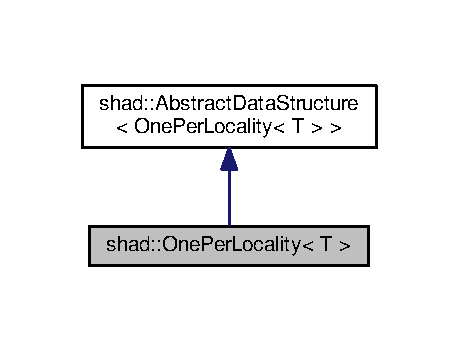
\includegraphics[width=220pt]{classshad_1_1OnePerLocality__inherit__graph}
\end{center}
\end{figure}


Collaboration diagram for shad\-:\-:One\-Per\-Locality$<$ T $>$\-:
\nopagebreak
\begin{figure}[H]
\begin{center}
\leavevmode
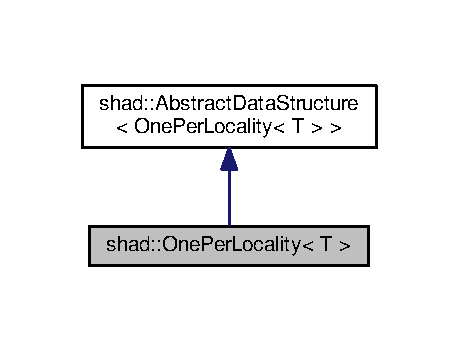
\includegraphics[width=220pt]{classshad_1_1OnePerLocality__coll__graph}
\end{center}
\end{figure}
\subsection*{Public Types}
\begin{DoxyCompactItemize}
\item 
using \hyperlink{classshad_1_1OnePerLocality_a60e8354048763662cb04eaab1b063977}{Object\-I\-D} = typename \hyperlink{classshad_1_1AbstractDataStructure}{Abstract\-Data\-Structure}$<$ \hyperlink{classshad_1_1OnePerLocality}{One\-Per\-Locality}$<$ T $>$$>$\-::\hyperlink{classshad_1_1OnePerLocality_a60e8354048763662cb04eaab1b063977}{Object\-I\-D}
\item 
using \hyperlink{classshad_1_1OnePerLocality_ad3a4f471e9d1fe8998bf783553c92d52}{Shared\-Ptr} = typename \hyperlink{classshad_1_1AbstractDataStructure}{Abstract\-Data\-Structure}$<$ \hyperlink{classshad_1_1OnePerLocality}{One\-Per\-Locality}$<$ T $>$$>$\-::\hyperlink{classshad_1_1OnePerLocality_ad3a4f471e9d1fe8998bf783553c92d52}{Shared\-Ptr}
\end{DoxyCompactItemize}
\subsection*{Public Member Functions}
\begin{DoxyCompactItemize}
\item 
\hyperlink{classshad_1_1OnePerLocality_a60e8354048763662cb04eaab1b063977}{Object\-I\-D} \hyperlink{classshad_1_1OnePerLocality_a83cb9589b89f27f1befc3ae669098c9c}{Get\-Global\-I\-D} () const 
\begin{DoxyCompactList}\small\item\em Retieve the Global Identifier. \end{DoxyCompactList}\item 
T $\ast$const \hyperlink{classshad_1_1OnePerLocality_a95a07b2c6d17140554f52112059b3d61}{operator-\/$>$} ()
\begin{DoxyCompactList}\small\item\em Access the local instance. \end{DoxyCompactList}\item 
\hyperlink{classshad_1_1OnePerLocality}{One\-Per\-Locality}$<$ T $>$ \& \hyperlink{classshad_1_1OnePerLocality_a82c608896e00521bffcba78fe7a0b88b}{operator=} (const T \&rhs)
\begin{DoxyCompactList}\small\item\em Assign the an instance of T to the local object. \end{DoxyCompactList}\item 
\hyperlink{classshad_1_1OnePerLocality_a721063d9435318f629e415b098643b19}{operator T} () const 
\begin{DoxyCompactList}\small\item\em Retrieve a copy of the local instance. \end{DoxyCompactList}\end{DoxyCompactItemize}
\subsection*{Static Public Member Functions}
\begin{DoxyCompactItemize}
\item 
{\footnotesize template$<$typename... Args$>$ }\\static \hyperlink{classshad_1_1OnePerLocality_ad3a4f471e9d1fe8998bf783553c92d52}{Shared\-Ptr} \hyperlink{classshad_1_1OnePerLocality_a16468f8c57a89f3419d977d9753b063b}{Create} (Args...\-args)
\begin{DoxyCompactList}\small\item\em Create method. \end{DoxyCompactList}\end{DoxyCompactItemize}
\subsection*{Protected Member Functions}
\begin{DoxyCompactItemize}
\item 
{\footnotesize template$<$typename... Args$>$ }\\\hyperlink{classshad_1_1OnePerLocality_ac33d20c6dd46594471d463c62b624190}{One\-Per\-Locality} (\hyperlink{classshad_1_1OnePerLocality_a60e8354048763662cb04eaab1b063977}{Object\-I\-D} oid, Args...\-args)
\begin{DoxyCompactList}\small\item\em Constructor. \end{DoxyCompactList}\end{DoxyCompactItemize}
\subsection*{Friends}
\begin{DoxyCompactItemize}
\item 
{\footnotesize template$<$typename $>$ }\\class \hyperlink{classshad_1_1OnePerLocality_ab18afa4496cc863ddc11bab94b2adf57}{Abstract\-Data\-Structure}
\end{DoxyCompactItemize}
\subsection*{Additional Inherited Members}


\subsection{Detailed Description}
\subsubsection*{template$<$typename T$>$class shad\-::\-One\-Per\-Locality$<$ T $>$}

Wrapper that instantiate one object per Locality in the system. 

This Wrapper triggers the instantiation of one object per Locality in the system.

\begin{DoxyWarning}{Warning}
Writes are not propagated across the system.
\end{DoxyWarning}

\begin{DoxyTemplParams}{Template Parameters}
{\em T} & The typen of the objects that will be instantiated. \\
\hline
\end{DoxyTemplParams}


\subsection{Member Typedef Documentation}
\hypertarget{classshad_1_1OnePerLocality_a60e8354048763662cb04eaab1b063977}{\index{shad\-::\-One\-Per\-Locality@{shad\-::\-One\-Per\-Locality}!Object\-I\-D@{Object\-I\-D}}
\index{Object\-I\-D@{Object\-I\-D}!shad::OnePerLocality@{shad\-::\-One\-Per\-Locality}}
\subsubsection[{Object\-I\-D}]{\setlength{\rightskip}{0pt plus 5cm}template$<$typename T $>$ using {\bf shad\-::\-One\-Per\-Locality}$<$ T $>$\-::{\bf Object\-I\-D} =  typename {\bf Abstract\-Data\-Structure}$<${\bf One\-Per\-Locality}$<$T$>$$>$\-::{\bf Object\-I\-D}}}\label{classshad_1_1OnePerLocality_a60e8354048763662cb04eaab1b063977}
\hypertarget{classshad_1_1OnePerLocality_ad3a4f471e9d1fe8998bf783553c92d52}{\index{shad\-::\-One\-Per\-Locality@{shad\-::\-One\-Per\-Locality}!Shared\-Ptr@{Shared\-Ptr}}
\index{Shared\-Ptr@{Shared\-Ptr}!shad::OnePerLocality@{shad\-::\-One\-Per\-Locality}}
\subsubsection[{Shared\-Ptr}]{\setlength{\rightskip}{0pt plus 5cm}template$<$typename T $>$ using {\bf shad\-::\-One\-Per\-Locality}$<$ T $>$\-::{\bf Shared\-Ptr} =  typename {\bf Abstract\-Data\-Structure}$<${\bf One\-Per\-Locality}$<$T$>$$>$\-::{\bf Shared\-Ptr}}}\label{classshad_1_1OnePerLocality_ad3a4f471e9d1fe8998bf783553c92d52}


\subsection{Constructor \& Destructor Documentation}
\hypertarget{classshad_1_1OnePerLocality_ac33d20c6dd46594471d463c62b624190}{\index{shad\-::\-One\-Per\-Locality@{shad\-::\-One\-Per\-Locality}!One\-Per\-Locality@{One\-Per\-Locality}}
\index{One\-Per\-Locality@{One\-Per\-Locality}!shad::OnePerLocality@{shad\-::\-One\-Per\-Locality}}
\subsubsection[{One\-Per\-Locality}]{\setlength{\rightskip}{0pt plus 5cm}template$<$typename T $>$ template$<$typename... Args$>$ {\bf shad\-::\-One\-Per\-Locality}$<$ T $>$\-::{\bf One\-Per\-Locality} (
\begin{DoxyParamCaption}
\item[{{\bf Object\-I\-D}}]{oid, }
\item[{Args...}]{args}
\end{DoxyParamCaption}
)\hspace{0.3cm}{\ttfamily [inline]}, {\ttfamily [explicit]}, {\ttfamily [protected]}}}\label{classshad_1_1OnePerLocality_ac33d20c6dd46594471d463c62b624190}


Constructor. 



\subsection{Member Function Documentation}
\hypertarget{classshad_1_1OnePerLocality_a16468f8c57a89f3419d977d9753b063b}{\index{shad\-::\-One\-Per\-Locality@{shad\-::\-One\-Per\-Locality}!Create@{Create}}
\index{Create@{Create}!shad::OnePerLocality@{shad\-::\-One\-Per\-Locality}}
\subsubsection[{Create}]{\setlength{\rightskip}{0pt plus 5cm}template$<$typename T $>$ template$<$typename... Args$>$ static {\bf Shared\-Ptr} {\bf shad\-::\-One\-Per\-Locality}$<$ T $>$\-::Create (
\begin{DoxyParamCaption}
\item[{Args...}]{args}
\end{DoxyParamCaption}
)\hspace{0.3cm}{\ttfamily [static]}}}\label{classshad_1_1OnePerLocality_a16468f8c57a89f3419d977d9753b063b}


Create method. 

Creates instances of a T object on each locality.


\begin{DoxyTemplParams}{Template Parameters}
{\em Args} & The list of types needed to build an instance of type T\\
\hline
\end{DoxyTemplParams}

\begin{DoxyParams}{Parameters}
{\em args} & The parameter pack to be forwarded to T' constructor. \\
\hline
\end{DoxyParams}
\begin{DoxyReturn}{Returns}
A shared pointer to the local One\-Perlocality instance. 
\end{DoxyReturn}
\hypertarget{classshad_1_1OnePerLocality_a83cb9589b89f27f1befc3ae669098c9c}{\index{shad\-::\-One\-Per\-Locality@{shad\-::\-One\-Per\-Locality}!Get\-Global\-I\-D@{Get\-Global\-I\-D}}
\index{Get\-Global\-I\-D@{Get\-Global\-I\-D}!shad::OnePerLocality@{shad\-::\-One\-Per\-Locality}}
\subsubsection[{Get\-Global\-I\-D}]{\setlength{\rightskip}{0pt plus 5cm}template$<$typename T $>$ {\bf Object\-I\-D} {\bf shad\-::\-One\-Per\-Locality}$<$ T $>$\-::Get\-Global\-I\-D (
\begin{DoxyParamCaption}
{}
\end{DoxyParamCaption}
) const\hspace{0.3cm}{\ttfamily [inline]}, {\ttfamily [virtual]}}}\label{classshad_1_1OnePerLocality_a83cb9589b89f27f1befc3ae669098c9c}


Retieve the Global Identifier. 

\begin{DoxyReturn}{Returns}
The global identifier associated with the array instance. 
\end{DoxyReturn}


Implements \hyperlink{classshad_1_1AbstractDataStructure_a914a6e24eec3a7f5d51d93323d3a39cc}{shad\-::\-Abstract\-Data\-Structure$<$ One\-Per\-Locality$<$ T $>$ $>$}.

\hypertarget{classshad_1_1OnePerLocality_a721063d9435318f629e415b098643b19}{\index{shad\-::\-One\-Per\-Locality@{shad\-::\-One\-Per\-Locality}!operator T@{operator T}}
\index{operator T@{operator T}!shad::OnePerLocality@{shad\-::\-One\-Per\-Locality}}
\subsubsection[{operator T}]{\setlength{\rightskip}{0pt plus 5cm}template$<$typename T $>$ {\bf shad\-::\-One\-Per\-Locality}$<$ T $>$\-::operator T (
\begin{DoxyParamCaption}
{}
\end{DoxyParamCaption}
) const\hspace{0.3cm}{\ttfamily [inline]}, {\ttfamily [explicit]}}}\label{classshad_1_1OnePerLocality_a721063d9435318f629e415b098643b19}


Retrieve a copy of the local instance. 

\hypertarget{classshad_1_1OnePerLocality_a95a07b2c6d17140554f52112059b3d61}{\index{shad\-::\-One\-Per\-Locality@{shad\-::\-One\-Per\-Locality}!operator-\/$>$@{operator-\/$>$}}
\index{operator-\/$>$@{operator-\/$>$}!shad::OnePerLocality@{shad\-::\-One\-Per\-Locality}}
\subsubsection[{operator-\/$>$}]{\setlength{\rightskip}{0pt plus 5cm}template$<$typename T $>$ T$\ast$ const {\bf shad\-::\-One\-Per\-Locality}$<$ T $>$\-::operator-\/$>$ (
\begin{DoxyParamCaption}
{}
\end{DoxyParamCaption}
)\hspace{0.3cm}{\ttfamily [inline]}}}\label{classshad_1_1OnePerLocality_a95a07b2c6d17140554f52112059b3d61}


Access the local instance. 

\begin{DoxyReturn}{Returns}
A pointer to the local instance. 
\end{DoxyReturn}
\hypertarget{classshad_1_1OnePerLocality_a82c608896e00521bffcba78fe7a0b88b}{\index{shad\-::\-One\-Per\-Locality@{shad\-::\-One\-Per\-Locality}!operator=@{operator=}}
\index{operator=@{operator=}!shad::OnePerLocality@{shad\-::\-One\-Per\-Locality}}
\subsubsection[{operator=}]{\setlength{\rightskip}{0pt plus 5cm}template$<$typename T $>$ {\bf One\-Per\-Locality}$<$T$>$\& {\bf shad\-::\-One\-Per\-Locality}$<$ T $>$\-::operator= (
\begin{DoxyParamCaption}
\item[{const T \&}]{rhs}
\end{DoxyParamCaption}
)\hspace{0.3cm}{\ttfamily [inline]}}}\label{classshad_1_1OnePerLocality_a82c608896e00521bffcba78fe7a0b88b}


Assign the an instance of T to the local object. 


\begin{DoxyTemplParams}{Template Parameters}
{\em T} & the type of the allocated. \\
\hline
\end{DoxyTemplParams}

\begin{DoxyParams}{Parameters}
{\em rhs} & The right-\/hand side of the assignment. \\
\hline
\end{DoxyParams}


\subsection{Friends And Related Function Documentation}
\hypertarget{classshad_1_1OnePerLocality_ab18afa4496cc863ddc11bab94b2adf57}{\index{shad\-::\-One\-Per\-Locality@{shad\-::\-One\-Per\-Locality}!Abstract\-Data\-Structure@{Abstract\-Data\-Structure}}
\index{Abstract\-Data\-Structure@{Abstract\-Data\-Structure}!shad::OnePerLocality@{shad\-::\-One\-Per\-Locality}}
\subsubsection[{Abstract\-Data\-Structure}]{\setlength{\rightskip}{0pt plus 5cm}template$<$typename T $>$ template$<$typename $>$ friend class {\bf Abstract\-Data\-Structure}\hspace{0.3cm}{\ttfamily [friend]}}}\label{classshad_1_1OnePerLocality_ab18afa4496cc863ddc11bab94b2adf57}


The documentation for this class was generated from the following file\-:\begin{DoxyCompactItemize}
\item 
include/shad/data\-\_\-structures/\hyperlink{one__per__locality_8h}{one\-\_\-per\-\_\-locality.\-h}\end{DoxyCompactItemize}

\hypertarget{structshad_1_1Overwriter}{\section{shad\-:\-:Overwriter$<$ T $>$ Struct Template Reference}
\label{structshad_1_1Overwriter}\index{shad\-::\-Overwriter$<$ T $>$@{shad\-::\-Overwriter$<$ T $>$}}
}


{\ttfamily \#include $<$shad/data\-\_\-structures/local\-\_\-hashmap.\-h$>$}

\subsection*{Public Member Functions}
\begin{DoxyCompactItemize}
\item 
bool \hyperlink{structshad_1_1Overwriter_afa430a0e2b445ff2f7bbd2b77e237bc0}{operator()} (T $\ast$const lhs, const T \&rhs, bool)
\end{DoxyCompactItemize}
\subsection*{Static Public Member Functions}
\begin{DoxyCompactItemize}
\item 
static bool \hyperlink{structshad_1_1Overwriter_a5e7bf0ee102f98373e29381e02fe133c}{Insert} (T $\ast$const lhs, const T \&rhs, bool)
\end{DoxyCompactItemize}


\subsection{Member Function Documentation}
\hypertarget{structshad_1_1Overwriter_a5e7bf0ee102f98373e29381e02fe133c}{\index{shad\-::\-Overwriter@{shad\-::\-Overwriter}!Insert@{Insert}}
\index{Insert@{Insert}!shad::Overwriter@{shad\-::\-Overwriter}}
\subsubsection[{Insert}]{\setlength{\rightskip}{0pt plus 5cm}template$<$typename T $>$ static bool {\bf shad\-::\-Overwriter}$<$ T $>$\-::Insert (
\begin{DoxyParamCaption}
\item[{T $\ast$const}]{lhs, }
\item[{const T \&}]{rhs, }
\item[{bool}]{}
\end{DoxyParamCaption}
)\hspace{0.3cm}{\ttfamily [inline]}, {\ttfamily [static]}}}\label{structshad_1_1Overwriter_a5e7bf0ee102f98373e29381e02fe133c}
\hypertarget{structshad_1_1Overwriter_afa430a0e2b445ff2f7bbd2b77e237bc0}{\index{shad\-::\-Overwriter@{shad\-::\-Overwriter}!operator()@{operator()}}
\index{operator()@{operator()}!shad::Overwriter@{shad\-::\-Overwriter}}
\subsubsection[{operator()}]{\setlength{\rightskip}{0pt plus 5cm}template$<$typename T $>$ bool {\bf shad\-::\-Overwriter}$<$ T $>$\-::operator() (
\begin{DoxyParamCaption}
\item[{T $\ast$const}]{lhs, }
\item[{const T \&}]{rhs, }
\item[{bool}]{}
\end{DoxyParamCaption}
)\hspace{0.3cm}{\ttfamily [inline]}}}\label{structshad_1_1Overwriter_afa430a0e2b445ff2f7bbd2b77e237bc0}


The documentation for this struct was generated from the following file\-:\begin{DoxyCompactItemize}
\item 
include/shad/data\-\_\-structures/\hyperlink{local__hashmap_8h}{local\-\_\-hashmap.\-h}\end{DoxyCompactItemize}

\hypertarget{classshad_1_1Set}{\section{shad\-:\-:Set$<$ T, E\-L\-E\-M\-\_\-\-C\-O\-M\-P\-A\-R\-E $>$ Class Template Reference}
\label{classshad_1_1Set}\index{shad\-::\-Set$<$ T, E\-L\-E\-M\-\_\-\-C\-O\-M\-P\-A\-R\-E $>$@{shad\-::\-Set$<$ T, E\-L\-E\-M\-\_\-\-C\-O\-M\-P\-A\-R\-E $>$}}
}


The \hyperlink{classshad_1_1Set}{Set} data structure.  




{\ttfamily \#include $<$shad/data\-\_\-structures/set.\-h$>$}



Inheritance diagram for shad\-:\-:Set$<$ T, E\-L\-E\-M\-\_\-\-C\-O\-M\-P\-A\-R\-E $>$\-:
\nopagebreak
\begin{figure}[H]
\begin{center}
\leavevmode
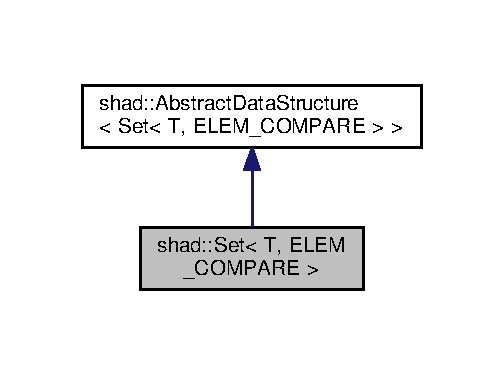
\includegraphics[width=242pt]{classshad_1_1Set__inherit__graph}
\end{center}
\end{figure}


Collaboration diagram for shad\-:\-:Set$<$ T, E\-L\-E\-M\-\_\-\-C\-O\-M\-P\-A\-R\-E $>$\-:
\nopagebreak
\begin{figure}[H]
\begin{center}
\leavevmode
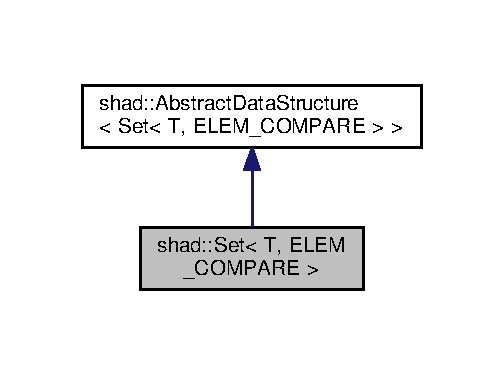
\includegraphics[width=242pt]{classshad_1_1Set__coll__graph}
\end{center}
\end{figure}
\subsection*{Public Types}
\begin{DoxyCompactItemize}
\item 
using \hyperlink{classshad_1_1Set_a20c26f02edb7c6c978a0e0b6f2b46c80}{value\-\_\-type} = T
\item 
using \hyperlink{classshad_1_1Set_ac4975698d3f73a58bb223e28ca582fa9}{Set\-T} = \hyperlink{classshad_1_1Set}{Set}$<$ T, E\-L\-E\-M\-\_\-\-C\-O\-M\-P\-A\-R\-E $>$
\item 
using \hyperlink{classshad_1_1Set_a93ad50cc28bbc3b48f87e69bfbf3c632}{L\-Set\-T} = \hyperlink{classshad_1_1LocalSet}{Local\-Set}$<$ T, E\-L\-E\-M\-\_\-\-C\-O\-M\-P\-A\-R\-E $>$
\item 
using \hyperlink{classshad_1_1Set_a05ba25e24c892602d707b21e3e4300b9}{Object\-I\-D} = typename \hyperlink{classshad_1_1AbstractDataStructure}{Abstract\-Data\-Structure}$<$ \hyperlink{classshad_1_1Set_ac4975698d3f73a58bb223e28ca582fa9}{Set\-T} $>$\-::\hyperlink{classshad_1_1Set_a05ba25e24c892602d707b21e3e4300b9}{Object\-I\-D}
\item 
using \hyperlink{classshad_1_1Set_aa35015620563a346ef29432143fe1f44}{Shad\-Set\-Ptr} = typename \hyperlink{classshad_1_1AbstractDataStructure}{Abstract\-Data\-Structure}$<$ \hyperlink{classshad_1_1Set_ac4975698d3f73a58bb223e28ca582fa9}{Set\-T} $>$\-::\hyperlink{classshad_1_1AbstractDataStructure_a8bb29450966955c546d40421ce46316f}{Shared\-Ptr}
\item 
using \hyperlink{classshad_1_1Set_ace82796db9a7938647d935452ea6d39c}{Buffers\-Vector} = typename impl\-::\-Buffers\-Vector$<$ T, \hyperlink{classshad_1_1Set_ac4975698d3f73a58bb223e28ca582fa9}{Set\-T} $>$
\item 
using \hyperlink{classshad_1_1Set_a726ddfe3c1c55db2ef60c5c1960d6666}{iterator} = \hyperlink{classshad_1_1set__iterator}{set\-\_\-iterator}$<$ \hyperlink{classshad_1_1Set}{Set}$<$ T, E\-L\-E\-M\-\_\-\-C\-O\-M\-P\-A\-R\-E $>$, T, T $>$
\item 
using \hyperlink{classshad_1_1Set_a0b2608f92f5397a25e62fad925fc177e}{const\-\_\-iterator} = \hyperlink{classshad_1_1set__iterator}{set\-\_\-iterator}$<$ \hyperlink{classshad_1_1Set}{Set}$<$ T, E\-L\-E\-M\-\_\-\-C\-O\-M\-P\-A\-R\-E $>$, const T, T $>$
\item 
using \hyperlink{classshad_1_1Set_a12ce7d6fd8fd0569035b0eb236b22179}{local\-\_\-iterator} = \hyperlink{classshad_1_1lset__iterator}{lset\-\_\-iterator}$<$ \hyperlink{classshad_1_1LocalSet}{Local\-Set}$<$ T, E\-L\-E\-M\-\_\-\-C\-O\-M\-P\-A\-R\-E $>$, T $>$
\item 
using \hyperlink{classshad_1_1Set_a0857d9ce7a249e860e3a67bc18f7de8b}{const\-\_\-local\-\_\-iterator} = \hyperlink{classshad_1_1lset__iterator}{lset\-\_\-iterator}$<$ \hyperlink{classshad_1_1LocalSet}{Local\-Set}$<$ T, E\-L\-E\-M\-\_\-\-C\-O\-M\-P\-A\-R\-E $>$, const T $>$
\end{DoxyCompactItemize}
\subsection*{Public Member Functions}
\begin{DoxyCompactItemize}
\item 
\hyperlink{classshad_1_1Set_a05ba25e24c892602d707b21e3e4300b9}{Object\-I\-D} \hyperlink{classshad_1_1Set_a4c57c459143fba4dc825e77217eb66c7}{Get\-Global\-I\-D} () const 
\begin{DoxyCompactList}\small\item\em Getter of the Global Identifier. \end{DoxyCompactList}\item 
size\-\_\-t \hyperlink{classshad_1_1Set_aefd9d547c7a8a720769e55cafc6802cf}{Size} () const 
\begin{DoxyCompactList}\small\item\em Overall size of the set (number of elements). \end{DoxyCompactList}\item 
void \hyperlink{classshad_1_1Set_a60e9b2e6a7aa74298897867f83851473}{Insert} (const T \&element)
\begin{DoxyCompactList}\small\item\em Insert an element in the set. \end{DoxyCompactList}\item 
void \hyperlink{classshad_1_1Set_a323831242d5737325df067e252c9d5b3}{Async\-Insert} (\hyperlink{classshad_1_1rt_1_1Handle}{rt\-::\-Handle} \&handle, const T \&element)
\begin{DoxyCompactList}\small\item\em Asynchronously Insert an element in the set. \end{DoxyCompactList}\item 
void \hyperlink{classshad_1_1Set_a1ac85f834d9ccd281f56c36742730e97}{Buffered\-Insert} (const T \&element)
\begin{DoxyCompactList}\small\item\em Buffered Insert method. Inserts an element, using aggregation buffers. \end{DoxyCompactList}\item 
void \hyperlink{classshad_1_1Set_a2d3f1919275884a863577853d05c64f2}{Buffered\-Async\-Insert} (\hyperlink{classshad_1_1rt_1_1Handle}{rt\-::\-Handle} \&handle, const T \&element)
\begin{DoxyCompactList}\small\item\em Asynchronous Buffered Insert method. Asynchronously inserts an element, using aggregation buffers. \end{DoxyCompactList}\item 
void \hyperlink{classshad_1_1Set_a3712197c5aaeadf247975051f81b03c7}{Wait\-For\-Buffered\-Insert} ()
\begin{DoxyCompactList}\small\item\em Finalize method for buffered insertions. \end{DoxyCompactList}\item 
void \hyperlink{classshad_1_1Set_a1d7269e2f1468f877d1efaac95e780e1}{Erase} (const T \&element)
\begin{DoxyCompactList}\small\item\em Remove an element from the set. \end{DoxyCompactList}\item 
void \hyperlink{classshad_1_1Set_ad424d2a53863f1228f245d57d8439842}{Async\-Erase} (\hyperlink{classshad_1_1rt_1_1Handle}{rt\-::\-Handle} \&handle, const T \&element)
\begin{DoxyCompactList}\small\item\em Asynchronously remove an element from the set. \end{DoxyCompactList}\item 
void \hyperlink{classshad_1_1Set_ad12b4cacd980e45c5cf77997917c17c1}{Clear} ()
\begin{DoxyCompactList}\small\item\em Clear the content of the set. \end{DoxyCompactList}\item 
void \hyperlink{classshad_1_1Set_a1af0696f3c2e3aea11fc04aaf39c7740}{Reset} (size\-\_\-t num\-Elements)
\begin{DoxyCompactList}\small\item\em Clear the content of the set. \end{DoxyCompactList}\item 
bool \hyperlink{classshad_1_1Set_a0a43db8a4eb3d76b5150d63e53c2ab50}{Find} (const T \&element)
\begin{DoxyCompactList}\small\item\em Check if the set contains a given element. \end{DoxyCompactList}\item 
void \hyperlink{classshad_1_1Set_afd802c9be7b268deafdc2ca6322e2a53}{Async\-Find} (\hyperlink{classshad_1_1rt_1_1Handle}{rt\-::\-Handle} \&handle, const T \&element, bool $\ast$found)
\begin{DoxyCompactList}\small\item\em Asynchronously check if the set contains a given element. \end{DoxyCompactList}\item 
{\footnotesize template$<$typename Apply\-Fun\-T , typename... Args$>$ }\\void \hyperlink{classshad_1_1Set_ae7ae217c231aa0ef54c5e2990c172b12}{For\-Each\-Element} (Apply\-Fun\-T \&\&function, Args \&...args)
\begin{DoxyCompactList}\small\item\em Apply a user-\/defined function to each element in the set. \end{DoxyCompactList}\item 
{\footnotesize template$<$typename Apply\-Fun\-T , typename... Args$>$ }\\void \hyperlink{classshad_1_1Set_ab4722765fe62737bd6b1b59635ebbe28}{Async\-For\-Each\-Element} (\hyperlink{classshad_1_1rt_1_1Handle}{rt\-::\-Handle} \&handle, Apply\-Fun\-T \&\&function, Args \&...args)
\begin{DoxyCompactList}\small\item\em Asynchronously apply a user-\/defined function to each element in the set. \end{DoxyCompactList}\item 
void \hyperlink{classshad_1_1Set_a92ae5af89da9c3232c062ecdacece447}{Print\-All\-Elements} ()
\begin{DoxyCompactList}\small\item\em Print all the entries in the set. \end{DoxyCompactList}\item 
void \hyperlink{classshad_1_1Set_aaa3c96b1f2eba65966ebc9e519adda01}{Buffer\-Entry\-Insert} (const T \&element)
\item 
\hyperlink{classshad_1_1Set_a726ddfe3c1c55db2ef60c5c1960d6666}{iterator} \hyperlink{classshad_1_1Set_ae747d10b913845091066d2393ea9695b}{begin} ()
\item 
\hyperlink{classshad_1_1Set_a726ddfe3c1c55db2ef60c5c1960d6666}{iterator} \hyperlink{classshad_1_1Set_a2e9ac1823ff085510d34773a0cb04852}{end} ()
\item 
\hyperlink{classshad_1_1Set_a0b2608f92f5397a25e62fad925fc177e}{const\-\_\-iterator} \hyperlink{classshad_1_1Set_ab486ba5133100428dbda82e28c3825db}{cbegin} ()
\item 
\hyperlink{classshad_1_1Set_a0b2608f92f5397a25e62fad925fc177e}{const\-\_\-iterator} \hyperlink{classshad_1_1Set_aa4e11c869e5268026f4d67d570808f0e}{cend} ()
\item 
\hyperlink{classshad_1_1Set_a12ce7d6fd8fd0569035b0eb236b22179}{local\-\_\-iterator} \hyperlink{classshad_1_1Set_a179918a1cbc5793a1522a00497495eeb}{local\-\_\-begin} ()
\item 
\hyperlink{classshad_1_1Set_a12ce7d6fd8fd0569035b0eb236b22179}{local\-\_\-iterator} \hyperlink{classshad_1_1Set_a274bae1a1e053109f42c8864bbc707e5}{local\-\_\-end} ()
\item 
\hyperlink{classshad_1_1Set_a0857d9ce7a249e860e3a67bc18f7de8b}{const\-\_\-local\-\_\-iterator} \hyperlink{classshad_1_1Set_af16201940dce366a4865b813031e8430}{clocal\-\_\-begin} ()
\item 
\hyperlink{classshad_1_1Set_a0857d9ce7a249e860e3a67bc18f7de8b}{const\-\_\-local\-\_\-iterator} \hyperlink{classshad_1_1Set_a9a4e1a99d244de6930a3e785fd2aedf3}{clocal\-\_\-end} ()
\end{DoxyCompactItemize}
\subsection*{Static Public Member Functions}
\begin{DoxyCompactItemize}
\item 
static \hyperlink{classshad_1_1Set_aa35015620563a346ef29432143fe1f44}{Shad\-Set\-Ptr} \hyperlink{classshad_1_1Set_a76419e199e1eb0b704f37bb4e5e107c9}{Create} (const size\-\_\-t num\-Entries)
\begin{DoxyCompactList}\small\item\em Create method. \end{DoxyCompactList}\end{DoxyCompactItemize}
\subsection*{Protected Member Functions}
\begin{DoxyCompactItemize}
\item 
\hyperlink{classshad_1_1Set_af23f31404ceabcf8c495c8dd77842c14}{Set} (\hyperlink{classshad_1_1Set_a05ba25e24c892602d707b21e3e4300b9}{Object\-I\-D} oid, const size\-\_\-t num\-Entries)
\end{DoxyCompactItemize}
\subsection*{Friends}
\begin{DoxyCompactItemize}
\item 
{\footnotesize template$<$typename $>$ }\\class \hyperlink{classshad_1_1Set_ab18afa4496cc863ddc11bab94b2adf57}{Abstract\-Data\-Structure}
\item 
class \hyperlink{classshad_1_1Set_a8a0a0fdcee0e492f8b2e3ad97cc1e397}{set\-\_\-iterator$<$ Set$<$ T, E\-L\-E\-M\-\_\-\-C\-O\-M\-P\-A\-R\-E $>$, T, T $>$}
\item 
class \hyperlink{classshad_1_1Set_a98fe017bca451c95c75b7e3d03b3d15a}{set\-\_\-iterator$<$ Set$<$ T, E\-L\-E\-M\-\_\-\-C\-O\-M\-P\-A\-R\-E $>$, const T, T $>$}
\end{DoxyCompactItemize}
\subsection*{Additional Inherited Members}


\subsection{Detailed Description}
\subsubsection*{template$<$typename T, typename E\-L\-E\-M\-\_\-\-C\-O\-M\-P\-A\-R\-E = Mem\-Cmp$<$\-T$>$$>$class shad\-::\-Set$<$ T, E\-L\-E\-M\-\_\-\-C\-O\-M\-P\-A\-R\-E $>$}

The \hyperlink{classshad_1_1Set}{Set} data structure. 

S\-H\-A\-D's set is a distributed, unordered, set. 
\begin{DoxyTemplParams}{Template Parameters}
{\em T} & type of the entries stored in the set. \\
\hline
{\em E\-L\-E\-M\-\_\-\-C\-O\-M\-P\-A\-R\-E} & element comparison function; default is Mem\-Cmp$<$\-T$>$. \\
\hline
\end{DoxyTemplParams}
\begin{DoxyWarning}{Warning}
obects of type T need to be trivially copiable. 
\end{DoxyWarning}


\subsection{Member Typedef Documentation}
\hypertarget{classshad_1_1Set_ace82796db9a7938647d935452ea6d39c}{\index{shad\-::\-Set@{shad\-::\-Set}!Buffers\-Vector@{Buffers\-Vector}}
\index{Buffers\-Vector@{Buffers\-Vector}!shad::Set@{shad\-::\-Set}}
\subsubsection[{Buffers\-Vector}]{\setlength{\rightskip}{0pt plus 5cm}template$<$typename T, typename E\-L\-E\-M\-\_\-\-C\-O\-M\-P\-A\-R\-E = Mem\-Cmp$<$\-T$>$$>$ using {\bf shad\-::\-Set}$<$ T, E\-L\-E\-M\-\_\-\-C\-O\-M\-P\-A\-R\-E $>$\-::{\bf Buffers\-Vector} =  typename impl\-::\-Buffers\-Vector$<$T, {\bf Set\-T}$>$}}\label{classshad_1_1Set_ace82796db9a7938647d935452ea6d39c}
\hypertarget{classshad_1_1Set_a0b2608f92f5397a25e62fad925fc177e}{\index{shad\-::\-Set@{shad\-::\-Set}!const\-\_\-iterator@{const\-\_\-iterator}}
\index{const\-\_\-iterator@{const\-\_\-iterator}!shad::Set@{shad\-::\-Set}}
\subsubsection[{const\-\_\-iterator}]{\setlength{\rightskip}{0pt plus 5cm}template$<$typename T, typename E\-L\-E\-M\-\_\-\-C\-O\-M\-P\-A\-R\-E = Mem\-Cmp$<$\-T$>$$>$ using {\bf shad\-::\-Set}$<$ T, E\-L\-E\-M\-\_\-\-C\-O\-M\-P\-A\-R\-E $>$\-::{\bf const\-\_\-iterator} =  {\bf set\-\_\-iterator}$<${\bf Set}$<$T, E\-L\-E\-M\-\_\-\-C\-O\-M\-P\-A\-R\-E$>$, const T, T$>$}}\label{classshad_1_1Set_a0b2608f92f5397a25e62fad925fc177e}
\hypertarget{classshad_1_1Set_a0857d9ce7a249e860e3a67bc18f7de8b}{\index{shad\-::\-Set@{shad\-::\-Set}!const\-\_\-local\-\_\-iterator@{const\-\_\-local\-\_\-iterator}}
\index{const\-\_\-local\-\_\-iterator@{const\-\_\-local\-\_\-iterator}!shad::Set@{shad\-::\-Set}}
\subsubsection[{const\-\_\-local\-\_\-iterator}]{\setlength{\rightskip}{0pt plus 5cm}template$<$typename T, typename E\-L\-E\-M\-\_\-\-C\-O\-M\-P\-A\-R\-E = Mem\-Cmp$<$\-T$>$$>$ using {\bf shad\-::\-Set}$<$ T, E\-L\-E\-M\-\_\-\-C\-O\-M\-P\-A\-R\-E $>$\-::{\bf const\-\_\-local\-\_\-iterator} =  {\bf lset\-\_\-iterator}$<${\bf Local\-Set}$<$T, E\-L\-E\-M\-\_\-\-C\-O\-M\-P\-A\-R\-E$>$, const T$>$}}\label{classshad_1_1Set_a0857d9ce7a249e860e3a67bc18f7de8b}
\hypertarget{classshad_1_1Set_a726ddfe3c1c55db2ef60c5c1960d6666}{\index{shad\-::\-Set@{shad\-::\-Set}!iterator@{iterator}}
\index{iterator@{iterator}!shad::Set@{shad\-::\-Set}}
\subsubsection[{iterator}]{\setlength{\rightskip}{0pt plus 5cm}template$<$typename T, typename E\-L\-E\-M\-\_\-\-C\-O\-M\-P\-A\-R\-E = Mem\-Cmp$<$\-T$>$$>$ using {\bf shad\-::\-Set}$<$ T, E\-L\-E\-M\-\_\-\-C\-O\-M\-P\-A\-R\-E $>$\-::{\bf iterator} =  {\bf set\-\_\-iterator}$<${\bf Set}$<$T, E\-L\-E\-M\-\_\-\-C\-O\-M\-P\-A\-R\-E$>$, T, T$>$}}\label{classshad_1_1Set_a726ddfe3c1c55db2ef60c5c1960d6666}
\hypertarget{classshad_1_1Set_a12ce7d6fd8fd0569035b0eb236b22179}{\index{shad\-::\-Set@{shad\-::\-Set}!local\-\_\-iterator@{local\-\_\-iterator}}
\index{local\-\_\-iterator@{local\-\_\-iterator}!shad::Set@{shad\-::\-Set}}
\subsubsection[{local\-\_\-iterator}]{\setlength{\rightskip}{0pt plus 5cm}template$<$typename T, typename E\-L\-E\-M\-\_\-\-C\-O\-M\-P\-A\-R\-E = Mem\-Cmp$<$\-T$>$$>$ using {\bf shad\-::\-Set}$<$ T, E\-L\-E\-M\-\_\-\-C\-O\-M\-P\-A\-R\-E $>$\-::{\bf local\-\_\-iterator} =  {\bf lset\-\_\-iterator}$<${\bf Local\-Set}$<$T, E\-L\-E\-M\-\_\-\-C\-O\-M\-P\-A\-R\-E$>$, T$>$}}\label{classshad_1_1Set_a12ce7d6fd8fd0569035b0eb236b22179}
\hypertarget{classshad_1_1Set_a93ad50cc28bbc3b48f87e69bfbf3c632}{\index{shad\-::\-Set@{shad\-::\-Set}!L\-Set\-T@{L\-Set\-T}}
\index{L\-Set\-T@{L\-Set\-T}!shad::Set@{shad\-::\-Set}}
\subsubsection[{L\-Set\-T}]{\setlength{\rightskip}{0pt plus 5cm}template$<$typename T, typename E\-L\-E\-M\-\_\-\-C\-O\-M\-P\-A\-R\-E = Mem\-Cmp$<$\-T$>$$>$ using {\bf shad\-::\-Set}$<$ T, E\-L\-E\-M\-\_\-\-C\-O\-M\-P\-A\-R\-E $>$\-::{\bf L\-Set\-T} =  {\bf Local\-Set}$<$T, E\-L\-E\-M\-\_\-\-C\-O\-M\-P\-A\-R\-E$>$}}\label{classshad_1_1Set_a93ad50cc28bbc3b48f87e69bfbf3c632}
\hypertarget{classshad_1_1Set_a05ba25e24c892602d707b21e3e4300b9}{\index{shad\-::\-Set@{shad\-::\-Set}!Object\-I\-D@{Object\-I\-D}}
\index{Object\-I\-D@{Object\-I\-D}!shad::Set@{shad\-::\-Set}}
\subsubsection[{Object\-I\-D}]{\setlength{\rightskip}{0pt plus 5cm}template$<$typename T, typename E\-L\-E\-M\-\_\-\-C\-O\-M\-P\-A\-R\-E = Mem\-Cmp$<$\-T$>$$>$ using {\bf shad\-::\-Set}$<$ T, E\-L\-E\-M\-\_\-\-C\-O\-M\-P\-A\-R\-E $>$\-::{\bf Object\-I\-D} =  typename {\bf Abstract\-Data\-Structure}$<${\bf Set\-T}$>$\-::{\bf Object\-I\-D}}}\label{classshad_1_1Set_a05ba25e24c892602d707b21e3e4300b9}
\hypertarget{classshad_1_1Set_ac4975698d3f73a58bb223e28ca582fa9}{\index{shad\-::\-Set@{shad\-::\-Set}!Set\-T@{Set\-T}}
\index{Set\-T@{Set\-T}!shad::Set@{shad\-::\-Set}}
\subsubsection[{Set\-T}]{\setlength{\rightskip}{0pt plus 5cm}template$<$typename T, typename E\-L\-E\-M\-\_\-\-C\-O\-M\-P\-A\-R\-E = Mem\-Cmp$<$\-T$>$$>$ using {\bf shad\-::\-Set}$<$ T, E\-L\-E\-M\-\_\-\-C\-O\-M\-P\-A\-R\-E $>$\-::{\bf Set\-T} =  {\bf Set}$<$T, E\-L\-E\-M\-\_\-\-C\-O\-M\-P\-A\-R\-E$>$}}\label{classshad_1_1Set_ac4975698d3f73a58bb223e28ca582fa9}
\hypertarget{classshad_1_1Set_aa35015620563a346ef29432143fe1f44}{\index{shad\-::\-Set@{shad\-::\-Set}!Shad\-Set\-Ptr@{Shad\-Set\-Ptr}}
\index{Shad\-Set\-Ptr@{Shad\-Set\-Ptr}!shad::Set@{shad\-::\-Set}}
\subsubsection[{Shad\-Set\-Ptr}]{\setlength{\rightskip}{0pt plus 5cm}template$<$typename T, typename E\-L\-E\-M\-\_\-\-C\-O\-M\-P\-A\-R\-E = Mem\-Cmp$<$\-T$>$$>$ using {\bf shad\-::\-Set}$<$ T, E\-L\-E\-M\-\_\-\-C\-O\-M\-P\-A\-R\-E $>$\-::{\bf Shad\-Set\-Ptr} =  typename {\bf Abstract\-Data\-Structure}$<${\bf Set\-T}$>$\-::{\bf Shared\-Ptr}}}\label{classshad_1_1Set_aa35015620563a346ef29432143fe1f44}
\hypertarget{classshad_1_1Set_a20c26f02edb7c6c978a0e0b6f2b46c80}{\index{shad\-::\-Set@{shad\-::\-Set}!value\-\_\-type@{value\-\_\-type}}
\index{value\-\_\-type@{value\-\_\-type}!shad::Set@{shad\-::\-Set}}
\subsubsection[{value\-\_\-type}]{\setlength{\rightskip}{0pt plus 5cm}template$<$typename T, typename E\-L\-E\-M\-\_\-\-C\-O\-M\-P\-A\-R\-E = Mem\-Cmp$<$\-T$>$$>$ using {\bf shad\-::\-Set}$<$ T, E\-L\-E\-M\-\_\-\-C\-O\-M\-P\-A\-R\-E $>$\-::{\bf value\-\_\-type} =  T}}\label{classshad_1_1Set_a20c26f02edb7c6c978a0e0b6f2b46c80}


\subsection{Constructor \& Destructor Documentation}
\hypertarget{classshad_1_1Set_af23f31404ceabcf8c495c8dd77842c14}{\index{shad\-::\-Set@{shad\-::\-Set}!Set@{Set}}
\index{Set@{Set}!shad::Set@{shad\-::\-Set}}
\subsubsection[{Set}]{\setlength{\rightskip}{0pt plus 5cm}template$<$typename T, typename E\-L\-E\-M\-\_\-\-C\-O\-M\-P\-A\-R\-E = Mem\-Cmp$<$\-T$>$$>$ {\bf shad\-::\-Set}$<$ T, E\-L\-E\-M\-\_\-\-C\-O\-M\-P\-A\-R\-E $>$\-::{\bf Set} (
\begin{DoxyParamCaption}
\item[{{\bf Object\-I\-D}}]{oid, }
\item[{const size\-\_\-t}]{num\-Entries}
\end{DoxyParamCaption}
)\hspace{0.3cm}{\ttfamily [inline]}, {\ttfamily [protected]}}}\label{classshad_1_1Set_af23f31404ceabcf8c495c8dd77842c14}


\subsection{Member Function Documentation}
\hypertarget{classshad_1_1Set_ad424d2a53863f1228f245d57d8439842}{\index{shad\-::\-Set@{shad\-::\-Set}!Async\-Erase@{Async\-Erase}}
\index{Async\-Erase@{Async\-Erase}!shad::Set@{shad\-::\-Set}}
\subsubsection[{Async\-Erase}]{\setlength{\rightskip}{0pt plus 5cm}template$<$typename T , typename E\-L\-E\-M\-\_\-\-C\-O\-M\-P\-A\-R\-E $>$ void {\bf shad\-::\-Set}$<$ T, E\-L\-E\-M\-\_\-\-C\-O\-M\-P\-A\-R\-E $>$\-::Async\-Erase (
\begin{DoxyParamCaption}
\item[{{\bf rt\-::\-Handle} \&}]{handle, }
\item[{const T \&}]{element}
\end{DoxyParamCaption}
)\hspace{0.3cm}{\ttfamily [inline]}}}\label{classshad_1_1Set_ad424d2a53863f1228f245d57d8439842}


Asynchronously remove an element from the set. 

\begin{DoxyWarning}{Warning}
Asynchronous operations are guaranteed to have completed only after calling the \hyperlink{namespaceshad_1_1rt_a6ea1d3672bac3a80032863b6732a0c0a}{rt\-::wait\-For\-Completion(rt\-::\-Handle \&handle)} method. 
\end{DoxyWarning}

\begin{DoxyParams}[1]{Parameters}
\mbox{\tt in,out}  & {\em handle} & Reference to the handle to be used to wait for completion. \\
\hline
\mbox{\tt in}  & {\em element} & the element. \\
\hline
\end{DoxyParams}
\hypertarget{classshad_1_1Set_afd802c9be7b268deafdc2ca6322e2a53}{\index{shad\-::\-Set@{shad\-::\-Set}!Async\-Find@{Async\-Find}}
\index{Async\-Find@{Async\-Find}!shad::Set@{shad\-::\-Set}}
\subsubsection[{Async\-Find}]{\setlength{\rightskip}{0pt plus 5cm}template$<$typename T , typename E\-L\-E\-M\-\_\-\-C\-O\-M\-P\-A\-R\-E $>$ void {\bf shad\-::\-Set}$<$ T, E\-L\-E\-M\-\_\-\-C\-O\-M\-P\-A\-R\-E $>$\-::Async\-Find (
\begin{DoxyParamCaption}
\item[{{\bf rt\-::\-Handle} \&}]{handle, }
\item[{const T \&}]{element, }
\item[{bool $\ast$}]{found}
\end{DoxyParamCaption}
)\hspace{0.3cm}{\ttfamily [inline]}}}\label{classshad_1_1Set_afd802c9be7b268deafdc2ca6322e2a53}


Asynchronously check if the set contains a given element. 

\begin{DoxyWarning}{Warning}
Asynchronous operations are guaranteed to have completed only after calling the \hyperlink{namespaceshad_1_1rt_a6ea1d3672bac3a80032863b6732a0c0a}{rt\-::wait\-For\-Completion(rt\-::\-Handle \&handle)} method. 
\end{DoxyWarning}

\begin{DoxyParams}[1]{Parameters}
\mbox{\tt in,out}  & {\em handle} & Reference to the handle to be used to wait for completion. \\
\hline
\mbox{\tt in}  & {\em element} & the element to find. \\
\hline
\mbox{\tt out}  & {\em found} & the address where to store the result of the operation. \\
\hline
\end{DoxyParams}
\hypertarget{classshad_1_1Set_ab4722765fe62737bd6b1b59635ebbe28}{\index{shad\-::\-Set@{shad\-::\-Set}!Async\-For\-Each\-Element@{Async\-For\-Each\-Element}}
\index{Async\-For\-Each\-Element@{Async\-For\-Each\-Element}!shad::Set@{shad\-::\-Set}}
\subsubsection[{Async\-For\-Each\-Element}]{\setlength{\rightskip}{0pt plus 5cm}template$<$typename T , typename E\-L\-E\-M\-\_\-\-C\-O\-M\-P\-A\-R\-E $>$ template$<$typename Apply\-Fun\-T , typename... Args$>$ void {\bf shad\-::\-Set}$<$ T, E\-L\-E\-M\-\_\-\-C\-O\-M\-P\-A\-R\-E $>$\-::Async\-For\-Each\-Element (
\begin{DoxyParamCaption}
\item[{{\bf rt\-::\-Handle} \&}]{handle, }
\item[{Apply\-Fun\-T \&\&}]{function, }
\item[{Args \&...}]{args}
\end{DoxyParamCaption}
)}}\label{classshad_1_1Set_ab4722765fe62737bd6b1b59635ebbe28}


Asynchronously apply a user-\/defined function to each element in the set. 


\begin{DoxyTemplParams}{Template Parameters}
{\em Apply\-Fun\-T} & User-\/defined function type. The function prototype should be\-: 
\begin{DoxyCode}
void(\hyperlink{classshad_1_1rt_1_1Handle}{shad::rt::Handle}&, \textcolor{keyword}{const} T&, Args&);
\end{DoxyCode}
 \\
\hline
{\em ...\-Args} & Types of the function arguments. \\
\hline
\end{DoxyTemplParams}
\begin{DoxyWarning}{Warning}
Asynchronous operations are guaranteed to have completed. only after calling the \hyperlink{namespaceshad_1_1rt_a6ea1d3672bac3a80032863b6732a0c0a}{rt\-::wait\-For\-Completion(rt\-::\-Handle \&handle)} method. 
\end{DoxyWarning}

\begin{DoxyParams}[1]{Parameters}
\mbox{\tt in,out}  & {\em handle} & Reference to the handle. to be used to wait for completion. \\
\hline
 & {\em function} & The function to apply. \\
\hline
 & {\em args} & The function arguments. \\
\hline
\end{DoxyParams}
\hypertarget{classshad_1_1Set_a323831242d5737325df067e252c9d5b3}{\index{shad\-::\-Set@{shad\-::\-Set}!Async\-Insert@{Async\-Insert}}
\index{Async\-Insert@{Async\-Insert}!shad::Set@{shad\-::\-Set}}
\subsubsection[{Async\-Insert}]{\setlength{\rightskip}{0pt plus 5cm}template$<$typename T , typename E\-L\-E\-M\-\_\-\-C\-O\-M\-P\-A\-R\-E $>$ void {\bf shad\-::\-Set}$<$ T, E\-L\-E\-M\-\_\-\-C\-O\-M\-P\-A\-R\-E $>$\-::Async\-Insert (
\begin{DoxyParamCaption}
\item[{{\bf rt\-::\-Handle} \&}]{handle, }
\item[{const T \&}]{element}
\end{DoxyParamCaption}
)\hspace{0.3cm}{\ttfamily [inline]}}}\label{classshad_1_1Set_a323831242d5737325df067e252c9d5b3}


Asynchronously Insert an element in the set. 

\begin{DoxyWarning}{Warning}
Asynchronous operations are guaranteed to have completed only after calling the \hyperlink{namespaceshad_1_1rt_a6ea1d3672bac3a80032863b6732a0c0a}{rt\-::wait\-For\-Completion(rt\-::\-Handle \&handle)} method. 
\end{DoxyWarning}

\begin{DoxyParams}[1]{Parameters}
\mbox{\tt in,out}  & {\em handle} & Reference to the handle to be used to wait for completion. \\
\hline
\mbox{\tt in}  & {\em element} & the element. \\
\hline
\end{DoxyParams}
\hypertarget{classshad_1_1Set_ae747d10b913845091066d2393ea9695b}{\index{shad\-::\-Set@{shad\-::\-Set}!begin@{begin}}
\index{begin@{begin}!shad::Set@{shad\-::\-Set}}
\subsubsection[{begin}]{\setlength{\rightskip}{0pt plus 5cm}template$<$typename T, typename E\-L\-E\-M\-\_\-\-C\-O\-M\-P\-A\-R\-E = Mem\-Cmp$<$\-T$>$$>$ {\bf iterator} {\bf shad\-::\-Set}$<$ T, E\-L\-E\-M\-\_\-\-C\-O\-M\-P\-A\-R\-E $>$\-::begin (
\begin{DoxyParamCaption}
{}
\end{DoxyParamCaption}
)\hspace{0.3cm}{\ttfamily [inline]}}}\label{classshad_1_1Set_ae747d10b913845091066d2393ea9695b}
\hypertarget{classshad_1_1Set_a2d3f1919275884a863577853d05c64f2}{\index{shad\-::\-Set@{shad\-::\-Set}!Buffered\-Async\-Insert@{Buffered\-Async\-Insert}}
\index{Buffered\-Async\-Insert@{Buffered\-Async\-Insert}!shad::Set@{shad\-::\-Set}}
\subsubsection[{Buffered\-Async\-Insert}]{\setlength{\rightskip}{0pt plus 5cm}template$<$typename T , typename E\-L\-E\-M\-\_\-\-C\-O\-M\-P\-A\-R\-E $>$ void {\bf shad\-::\-Set}$<$ T, E\-L\-E\-M\-\_\-\-C\-O\-M\-P\-A\-R\-E $>$\-::Buffered\-Async\-Insert (
\begin{DoxyParamCaption}
\item[{{\bf rt\-::\-Handle} \&}]{handle, }
\item[{const T \&}]{element}
\end{DoxyParamCaption}
)\hspace{0.3cm}{\ttfamily [inline]}}}\label{classshad_1_1Set_a2d3f1919275884a863577853d05c64f2}


Asynchronous Buffered Insert method. Asynchronously inserts an element, using aggregation buffers. 

\begin{DoxyWarning}{Warning}
asynchronous buffered insertions are finalized only after calling the \hyperlink{namespaceshad_1_1rt_a6ea1d3672bac3a80032863b6732a0c0a}{rt\-::wait\-For\-Completion(rt\-::\-Handle \&handle)} method A\-N\-D the \hyperlink{classshad_1_1Set_a3712197c5aaeadf247975051f81b03c7}{Wait\-For\-Buffered\-Insert()} method, in this order. 
\end{DoxyWarning}

\begin{DoxyParams}[1]{Parameters}
\mbox{\tt in,out}  & {\em handle} & Reference to the handle \\
\hline
\mbox{\tt in}  & {\em element} & The element. \\
\hline
\end{DoxyParams}
\hypertarget{classshad_1_1Set_a1ac85f834d9ccd281f56c36742730e97}{\index{shad\-::\-Set@{shad\-::\-Set}!Buffered\-Insert@{Buffered\-Insert}}
\index{Buffered\-Insert@{Buffered\-Insert}!shad::Set@{shad\-::\-Set}}
\subsubsection[{Buffered\-Insert}]{\setlength{\rightskip}{0pt plus 5cm}template$<$typename T , typename E\-L\-E\-M\-\_\-\-C\-O\-M\-P\-A\-R\-E $>$ void {\bf shad\-::\-Set}$<$ T, E\-L\-E\-M\-\_\-\-C\-O\-M\-P\-A\-R\-E $>$\-::Buffered\-Insert (
\begin{DoxyParamCaption}
\item[{const T \&}]{element}
\end{DoxyParamCaption}
)\hspace{0.3cm}{\ttfamily [inline]}}}\label{classshad_1_1Set_a1ac85f834d9ccd281f56c36742730e97}


Buffered Insert method. Inserts an element, using aggregation buffers. 

\begin{DoxyWarning}{Warning}
Insertions are finalized only after calling the \hyperlink{classshad_1_1Set_a3712197c5aaeadf247975051f81b03c7}{Wait\-For\-Buffered\-Insert()} method. 
\end{DoxyWarning}

\begin{DoxyParams}[1]{Parameters}
\mbox{\tt in}  & {\em element} & The element. \\
\hline
\end{DoxyParams}
\hypertarget{classshad_1_1Set_aaa3c96b1f2eba65966ebc9e519adda01}{\index{shad\-::\-Set@{shad\-::\-Set}!Buffer\-Entry\-Insert@{Buffer\-Entry\-Insert}}
\index{Buffer\-Entry\-Insert@{Buffer\-Entry\-Insert}!shad::Set@{shad\-::\-Set}}
\subsubsection[{Buffer\-Entry\-Insert}]{\setlength{\rightskip}{0pt plus 5cm}template$<$typename T, typename E\-L\-E\-M\-\_\-\-C\-O\-M\-P\-A\-R\-E = Mem\-Cmp$<$\-T$>$$>$ void {\bf shad\-::\-Set}$<$ T, E\-L\-E\-M\-\_\-\-C\-O\-M\-P\-A\-R\-E $>$\-::Buffer\-Entry\-Insert (
\begin{DoxyParamCaption}
\item[{const T \&}]{element}
\end{DoxyParamCaption}
)\hspace{0.3cm}{\ttfamily [inline]}}}\label{classshad_1_1Set_aaa3c96b1f2eba65966ebc9e519adda01}
\hypertarget{classshad_1_1Set_ab486ba5133100428dbda82e28c3825db}{\index{shad\-::\-Set@{shad\-::\-Set}!cbegin@{cbegin}}
\index{cbegin@{cbegin}!shad::Set@{shad\-::\-Set}}
\subsubsection[{cbegin}]{\setlength{\rightskip}{0pt plus 5cm}template$<$typename T, typename E\-L\-E\-M\-\_\-\-C\-O\-M\-P\-A\-R\-E = Mem\-Cmp$<$\-T$>$$>$ {\bf const\-\_\-iterator} {\bf shad\-::\-Set}$<$ T, E\-L\-E\-M\-\_\-\-C\-O\-M\-P\-A\-R\-E $>$\-::cbegin (
\begin{DoxyParamCaption}
{}
\end{DoxyParamCaption}
)\hspace{0.3cm}{\ttfamily [inline]}}}\label{classshad_1_1Set_ab486ba5133100428dbda82e28c3825db}
\hypertarget{classshad_1_1Set_aa4e11c869e5268026f4d67d570808f0e}{\index{shad\-::\-Set@{shad\-::\-Set}!cend@{cend}}
\index{cend@{cend}!shad::Set@{shad\-::\-Set}}
\subsubsection[{cend}]{\setlength{\rightskip}{0pt plus 5cm}template$<$typename T, typename E\-L\-E\-M\-\_\-\-C\-O\-M\-P\-A\-R\-E = Mem\-Cmp$<$\-T$>$$>$ {\bf const\-\_\-iterator} {\bf shad\-::\-Set}$<$ T, E\-L\-E\-M\-\_\-\-C\-O\-M\-P\-A\-R\-E $>$\-::cend (
\begin{DoxyParamCaption}
{}
\end{DoxyParamCaption}
)\hspace{0.3cm}{\ttfamily [inline]}}}\label{classshad_1_1Set_aa4e11c869e5268026f4d67d570808f0e}
\hypertarget{classshad_1_1Set_ad12b4cacd980e45c5cf77997917c17c1}{\index{shad\-::\-Set@{shad\-::\-Set}!Clear@{Clear}}
\index{Clear@{Clear}!shad::Set@{shad\-::\-Set}}
\subsubsection[{Clear}]{\setlength{\rightskip}{0pt plus 5cm}template$<$typename T, typename E\-L\-E\-M\-\_\-\-C\-O\-M\-P\-A\-R\-E = Mem\-Cmp$<$\-T$>$$>$ void {\bf shad\-::\-Set}$<$ T, E\-L\-E\-M\-\_\-\-C\-O\-M\-P\-A\-R\-E $>$\-::Clear (
\begin{DoxyParamCaption}
{}
\end{DoxyParamCaption}
)\hspace{0.3cm}{\ttfamily [inline]}}}\label{classshad_1_1Set_ad12b4cacd980e45c5cf77997917c17c1}


Clear the content of the set. 

\hypertarget{classshad_1_1Set_af16201940dce366a4865b813031e8430}{\index{shad\-::\-Set@{shad\-::\-Set}!clocal\-\_\-begin@{clocal\-\_\-begin}}
\index{clocal\-\_\-begin@{clocal\-\_\-begin}!shad::Set@{shad\-::\-Set}}
\subsubsection[{clocal\-\_\-begin}]{\setlength{\rightskip}{0pt plus 5cm}template$<$typename T, typename E\-L\-E\-M\-\_\-\-C\-O\-M\-P\-A\-R\-E = Mem\-Cmp$<$\-T$>$$>$ {\bf const\-\_\-local\-\_\-iterator} {\bf shad\-::\-Set}$<$ T, E\-L\-E\-M\-\_\-\-C\-O\-M\-P\-A\-R\-E $>$\-::clocal\-\_\-begin (
\begin{DoxyParamCaption}
{}
\end{DoxyParamCaption}
)\hspace{0.3cm}{\ttfamily [inline]}}}\label{classshad_1_1Set_af16201940dce366a4865b813031e8430}
\hypertarget{classshad_1_1Set_a9a4e1a99d244de6930a3e785fd2aedf3}{\index{shad\-::\-Set@{shad\-::\-Set}!clocal\-\_\-end@{clocal\-\_\-end}}
\index{clocal\-\_\-end@{clocal\-\_\-end}!shad::Set@{shad\-::\-Set}}
\subsubsection[{clocal\-\_\-end}]{\setlength{\rightskip}{0pt plus 5cm}template$<$typename T, typename E\-L\-E\-M\-\_\-\-C\-O\-M\-P\-A\-R\-E = Mem\-Cmp$<$\-T$>$$>$ {\bf const\-\_\-local\-\_\-iterator} {\bf shad\-::\-Set}$<$ T, E\-L\-E\-M\-\_\-\-C\-O\-M\-P\-A\-R\-E $>$\-::clocal\-\_\-end (
\begin{DoxyParamCaption}
{}
\end{DoxyParamCaption}
)\hspace{0.3cm}{\ttfamily [inline]}}}\label{classshad_1_1Set_a9a4e1a99d244de6930a3e785fd2aedf3}
\hypertarget{classshad_1_1Set_a76419e199e1eb0b704f37bb4e5e107c9}{\index{shad\-::\-Set@{shad\-::\-Set}!Create@{Create}}
\index{Create@{Create}!shad::Set@{shad\-::\-Set}}
\subsubsection[{Create}]{\setlength{\rightskip}{0pt plus 5cm}template$<$typename T, typename E\-L\-E\-M\-\_\-\-C\-O\-M\-P\-A\-R\-E = Mem\-Cmp$<$\-T$>$$>$ static {\bf Shad\-Set\-Ptr} {\bf shad\-::\-Set}$<$ T, E\-L\-E\-M\-\_\-\-C\-O\-M\-P\-A\-R\-E $>$\-::Create (
\begin{DoxyParamCaption}
\item[{const size\-\_\-t}]{num\-Entries}
\end{DoxyParamCaption}
)\hspace{0.3cm}{\ttfamily [static]}}}\label{classshad_1_1Set_a76419e199e1eb0b704f37bb4e5e107c9}


Create method. 

Creates a new set instance. 
\begin{DoxyParams}{Parameters}
{\em num\-Entries} & Expected number of elements. \\
\hline
\end{DoxyParams}
\begin{DoxyReturn}{Returns}
A shared pointer to the newly created set instance. 
\end{DoxyReturn}
\hypertarget{classshad_1_1Set_a2e9ac1823ff085510d34773a0cb04852}{\index{shad\-::\-Set@{shad\-::\-Set}!end@{end}}
\index{end@{end}!shad::Set@{shad\-::\-Set}}
\subsubsection[{end}]{\setlength{\rightskip}{0pt plus 5cm}template$<$typename T, typename E\-L\-E\-M\-\_\-\-C\-O\-M\-P\-A\-R\-E = Mem\-Cmp$<$\-T$>$$>$ {\bf iterator} {\bf shad\-::\-Set}$<$ T, E\-L\-E\-M\-\_\-\-C\-O\-M\-P\-A\-R\-E $>$\-::end (
\begin{DoxyParamCaption}
{}
\end{DoxyParamCaption}
)\hspace{0.3cm}{\ttfamily [inline]}}}\label{classshad_1_1Set_a2e9ac1823ff085510d34773a0cb04852}
\hypertarget{classshad_1_1Set_a1d7269e2f1468f877d1efaac95e780e1}{\index{shad\-::\-Set@{shad\-::\-Set}!Erase@{Erase}}
\index{Erase@{Erase}!shad::Set@{shad\-::\-Set}}
\subsubsection[{Erase}]{\setlength{\rightskip}{0pt plus 5cm}template$<$typename T , typename E\-L\-E\-M\-\_\-\-C\-O\-M\-P\-A\-R\-E $>$ void {\bf shad\-::\-Set}$<$ T, E\-L\-E\-M\-\_\-\-C\-O\-M\-P\-A\-R\-E $>$\-::Erase (
\begin{DoxyParamCaption}
\item[{const T \&}]{element}
\end{DoxyParamCaption}
)\hspace{0.3cm}{\ttfamily [inline]}}}\label{classshad_1_1Set_a1d7269e2f1468f877d1efaac95e780e1}


Remove an element from the set. 


\begin{DoxyParams}[1]{Parameters}
\mbox{\tt in}  & {\em element} & the element. \\
\hline
\end{DoxyParams}
\hypertarget{classshad_1_1Set_a0a43db8a4eb3d76b5150d63e53c2ab50}{\index{shad\-::\-Set@{shad\-::\-Set}!Find@{Find}}
\index{Find@{Find}!shad::Set@{shad\-::\-Set}}
\subsubsection[{Find}]{\setlength{\rightskip}{0pt plus 5cm}template$<$typename T , typename E\-L\-E\-M\-\_\-\-C\-O\-M\-P\-A\-R\-E $>$ bool {\bf shad\-::\-Set}$<$ T, E\-L\-E\-M\-\_\-\-C\-O\-M\-P\-A\-R\-E $>$\-::Find (
\begin{DoxyParamCaption}
\item[{const T \&}]{element}
\end{DoxyParamCaption}
)\hspace{0.3cm}{\ttfamily [inline]}}}\label{classshad_1_1Set_a0a43db8a4eb3d76b5150d63e53c2ab50}


Check if the set contains a given element. 


\begin{DoxyParams}[1]{Parameters}
\mbox{\tt in}  & {\em element} & the element to find. \\
\hline
\end{DoxyParams}
\begin{DoxyReturn}{Returns}
true if the element is found, false otherwise. 
\end{DoxyReturn}
\hypertarget{classshad_1_1Set_ae7ae217c231aa0ef54c5e2990c172b12}{\index{shad\-::\-Set@{shad\-::\-Set}!For\-Each\-Element@{For\-Each\-Element}}
\index{For\-Each\-Element@{For\-Each\-Element}!shad::Set@{shad\-::\-Set}}
\subsubsection[{For\-Each\-Element}]{\setlength{\rightskip}{0pt plus 5cm}template$<$typename T , typename E\-L\-E\-M\-\_\-\-C\-O\-M\-P\-A\-R\-E $>$ template$<$typename Apply\-Fun\-T , typename... Args$>$ void {\bf shad\-::\-Set}$<$ T, E\-L\-E\-M\-\_\-\-C\-O\-M\-P\-A\-R\-E $>$\-::For\-Each\-Element (
\begin{DoxyParamCaption}
\item[{Apply\-Fun\-T \&\&}]{function, }
\item[{Args \&...}]{args}
\end{DoxyParamCaption}
)}}\label{classshad_1_1Set_ae7ae217c231aa0ef54c5e2990c172b12}


Apply a user-\/defined function to each element in the set. 


\begin{DoxyTemplParams}{Template Parameters}
{\em Apply\-Fun\-T} & User-\/defined function type. The function prototype should be\-: 
\begin{DoxyCode}
void(\textcolor{keyword}{const} T&, Args&);
\end{DoxyCode}
 \\
\hline
{\em ...\-Args} & Types of the function arguments. \\
\hline
\end{DoxyTemplParams}

\begin{DoxyParams}{Parameters}
{\em function} & The function to apply. \\
\hline
{\em args} & The function arguments. \\
\hline
\end{DoxyParams}
\hypertarget{classshad_1_1Set_a4c57c459143fba4dc825e77217eb66c7}{\index{shad\-::\-Set@{shad\-::\-Set}!Get\-Global\-I\-D@{Get\-Global\-I\-D}}
\index{Get\-Global\-I\-D@{Get\-Global\-I\-D}!shad::Set@{shad\-::\-Set}}
\subsubsection[{Get\-Global\-I\-D}]{\setlength{\rightskip}{0pt plus 5cm}template$<$typename T, typename E\-L\-E\-M\-\_\-\-C\-O\-M\-P\-A\-R\-E = Mem\-Cmp$<$\-T$>$$>$ {\bf Object\-I\-D} {\bf shad\-::\-Set}$<$ T, E\-L\-E\-M\-\_\-\-C\-O\-M\-P\-A\-R\-E $>$\-::Get\-Global\-I\-D (
\begin{DoxyParamCaption}
{}
\end{DoxyParamCaption}
) const\hspace{0.3cm}{\ttfamily [inline]}, {\ttfamily [virtual]}}}\label{classshad_1_1Set_a4c57c459143fba4dc825e77217eb66c7}


Getter of the Global Identifier. 

\begin{DoxyReturn}{Returns}
The global identifier associated with the set instance. 
\end{DoxyReturn}


Implements \hyperlink{classshad_1_1AbstractDataStructure_a914a6e24eec3a7f5d51d93323d3a39cc}{shad\-::\-Abstract\-Data\-Structure$<$ Set$<$ T, E\-L\-E\-M\-\_\-\-C\-O\-M\-P\-A\-R\-E $>$ $>$}.

\hypertarget{classshad_1_1Set_a60e9b2e6a7aa74298897867f83851473}{\index{shad\-::\-Set@{shad\-::\-Set}!Insert@{Insert}}
\index{Insert@{Insert}!shad::Set@{shad\-::\-Set}}
\subsubsection[{Insert}]{\setlength{\rightskip}{0pt plus 5cm}template$<$typename T , typename E\-L\-E\-M\-\_\-\-C\-O\-M\-P\-A\-R\-E $>$ void {\bf shad\-::\-Set}$<$ T, E\-L\-E\-M\-\_\-\-C\-O\-M\-P\-A\-R\-E $>$\-::Insert (
\begin{DoxyParamCaption}
\item[{const T \&}]{element}
\end{DoxyParamCaption}
)\hspace{0.3cm}{\ttfamily [inline]}}}\label{classshad_1_1Set_a60e9b2e6a7aa74298897867f83851473}


Insert an element in the set. 


\begin{DoxyParams}[1]{Parameters}
\mbox{\tt in}  & {\em element} & the element. \\
\hline
\end{DoxyParams}
\hypertarget{classshad_1_1Set_a179918a1cbc5793a1522a00497495eeb}{\index{shad\-::\-Set@{shad\-::\-Set}!local\-\_\-begin@{local\-\_\-begin}}
\index{local\-\_\-begin@{local\-\_\-begin}!shad::Set@{shad\-::\-Set}}
\subsubsection[{local\-\_\-begin}]{\setlength{\rightskip}{0pt plus 5cm}template$<$typename T, typename E\-L\-E\-M\-\_\-\-C\-O\-M\-P\-A\-R\-E = Mem\-Cmp$<$\-T$>$$>$ {\bf local\-\_\-iterator} {\bf shad\-::\-Set}$<$ T, E\-L\-E\-M\-\_\-\-C\-O\-M\-P\-A\-R\-E $>$\-::local\-\_\-begin (
\begin{DoxyParamCaption}
{}
\end{DoxyParamCaption}
)\hspace{0.3cm}{\ttfamily [inline]}}}\label{classshad_1_1Set_a179918a1cbc5793a1522a00497495eeb}
\hypertarget{classshad_1_1Set_a274bae1a1e053109f42c8864bbc707e5}{\index{shad\-::\-Set@{shad\-::\-Set}!local\-\_\-end@{local\-\_\-end}}
\index{local\-\_\-end@{local\-\_\-end}!shad::Set@{shad\-::\-Set}}
\subsubsection[{local\-\_\-end}]{\setlength{\rightskip}{0pt plus 5cm}template$<$typename T, typename E\-L\-E\-M\-\_\-\-C\-O\-M\-P\-A\-R\-E = Mem\-Cmp$<$\-T$>$$>$ {\bf local\-\_\-iterator} {\bf shad\-::\-Set}$<$ T, E\-L\-E\-M\-\_\-\-C\-O\-M\-P\-A\-R\-E $>$\-::local\-\_\-end (
\begin{DoxyParamCaption}
{}
\end{DoxyParamCaption}
)\hspace{0.3cm}{\ttfamily [inline]}}}\label{classshad_1_1Set_a274bae1a1e053109f42c8864bbc707e5}
\hypertarget{classshad_1_1Set_a92ae5af89da9c3232c062ecdacece447}{\index{shad\-::\-Set@{shad\-::\-Set}!Print\-All\-Elements@{Print\-All\-Elements}}
\index{Print\-All\-Elements@{Print\-All\-Elements}!shad::Set@{shad\-::\-Set}}
\subsubsection[{Print\-All\-Elements}]{\setlength{\rightskip}{0pt plus 5cm}template$<$typename T, typename E\-L\-E\-M\-\_\-\-C\-O\-M\-P\-A\-R\-E = Mem\-Cmp$<$\-T$>$$>$ void {\bf shad\-::\-Set}$<$ T, E\-L\-E\-M\-\_\-\-C\-O\-M\-P\-A\-R\-E $>$\-::Print\-All\-Elements (
\begin{DoxyParamCaption}
{}
\end{DoxyParamCaption}
)\hspace{0.3cm}{\ttfamily [inline]}}}\label{classshad_1_1Set_a92ae5af89da9c3232c062ecdacece447}


Print all the entries in the set. 

\begin{DoxyWarning}{Warning}
std\-::ostream \& operator$<$$<$ must be defined for T. 
\end{DoxyWarning}
\hypertarget{classshad_1_1Set_a1af0696f3c2e3aea11fc04aaf39c7740}{\index{shad\-::\-Set@{shad\-::\-Set}!Reset@{Reset}}
\index{Reset@{Reset}!shad::Set@{shad\-::\-Set}}
\subsubsection[{Reset}]{\setlength{\rightskip}{0pt plus 5cm}template$<$typename T, typename E\-L\-E\-M\-\_\-\-C\-O\-M\-P\-A\-R\-E = Mem\-Cmp$<$\-T$>$$>$ void {\bf shad\-::\-Set}$<$ T, E\-L\-E\-M\-\_\-\-C\-O\-M\-P\-A\-R\-E $>$\-::Reset (
\begin{DoxyParamCaption}
\item[{size\-\_\-t}]{num\-Elements}
\end{DoxyParamCaption}
)\hspace{0.3cm}{\ttfamily [inline]}}}\label{classshad_1_1Set_a1af0696f3c2e3aea11fc04aaf39c7740}


Clear the content of the set. 

\hypertarget{classshad_1_1Set_aefd9d547c7a8a720769e55cafc6802cf}{\index{shad\-::\-Set@{shad\-::\-Set}!Size@{Size}}
\index{Size@{Size}!shad::Set@{shad\-::\-Set}}
\subsubsection[{Size}]{\setlength{\rightskip}{0pt plus 5cm}template$<$typename T , typename E\-L\-E\-M\-\_\-\-C\-O\-M\-P\-A\-R\-E $>$ size\-\_\-t {\bf shad\-::\-Set}$<$ T, E\-L\-E\-M\-\_\-\-C\-O\-M\-P\-A\-R\-E $>$\-::Size (
\begin{DoxyParamCaption}
{}
\end{DoxyParamCaption}
) const\hspace{0.3cm}{\ttfamily [inline]}}}\label{classshad_1_1Set_aefd9d547c7a8a720769e55cafc6802cf}


Overall size of the set (number of elements). 

\begin{DoxyWarning}{Warning}
Calling the size method may result in one-\/to-\/all communication among localities to retrieve consinstent information. 
\end{DoxyWarning}
\begin{DoxyReturn}{Returns}
the size of the set. 
\end{DoxyReturn}
\hypertarget{classshad_1_1Set_a3712197c5aaeadf247975051f81b03c7}{\index{shad\-::\-Set@{shad\-::\-Set}!Wait\-For\-Buffered\-Insert@{Wait\-For\-Buffered\-Insert}}
\index{Wait\-For\-Buffered\-Insert@{Wait\-For\-Buffered\-Insert}!shad::Set@{shad\-::\-Set}}
\subsubsection[{Wait\-For\-Buffered\-Insert}]{\setlength{\rightskip}{0pt plus 5cm}template$<$typename T, typename E\-L\-E\-M\-\_\-\-C\-O\-M\-P\-A\-R\-E = Mem\-Cmp$<$\-T$>$$>$ void {\bf shad\-::\-Set}$<$ T, E\-L\-E\-M\-\_\-\-C\-O\-M\-P\-A\-R\-E $>$\-::Wait\-For\-Buffered\-Insert (
\begin{DoxyParamCaption}
{}
\end{DoxyParamCaption}
)\hspace{0.3cm}{\ttfamily [inline]}}}\label{classshad_1_1Set_a3712197c5aaeadf247975051f81b03c7}


Finalize method for buffered insertions. 



\subsection{Friends And Related Function Documentation}
\hypertarget{classshad_1_1Set_ab18afa4496cc863ddc11bab94b2adf57}{\index{shad\-::\-Set@{shad\-::\-Set}!Abstract\-Data\-Structure@{Abstract\-Data\-Structure}}
\index{Abstract\-Data\-Structure@{Abstract\-Data\-Structure}!shad::Set@{shad\-::\-Set}}
\subsubsection[{Abstract\-Data\-Structure}]{\setlength{\rightskip}{0pt plus 5cm}template$<$typename T, typename E\-L\-E\-M\-\_\-\-C\-O\-M\-P\-A\-R\-E = Mem\-Cmp$<$\-T$>$$>$ template$<$typename $>$ friend class {\bf Abstract\-Data\-Structure}\hspace{0.3cm}{\ttfamily [friend]}}}\label{classshad_1_1Set_ab18afa4496cc863ddc11bab94b2adf57}
\hypertarget{classshad_1_1Set_a98fe017bca451c95c75b7e3d03b3d15a}{\index{shad\-::\-Set@{shad\-::\-Set}!set\-\_\-iterator$<$ Set$<$ T, E\-L\-E\-M\-\_\-\-C\-O\-M\-P\-A\-R\-E $>$, const T, T $>$@{set\-\_\-iterator$<$ Set$<$ T, E\-L\-E\-M\-\_\-\-C\-O\-M\-P\-A\-R\-E $>$, const T, T $>$}}
\index{set\-\_\-iterator$<$ Set$<$ T, E\-L\-E\-M\-\_\-\-C\-O\-M\-P\-A\-R\-E $>$, const T, T $>$@{set\-\_\-iterator$<$ Set$<$ T, E\-L\-E\-M\-\_\-\-C\-O\-M\-P\-A\-R\-E $>$, const T, T $>$}!shad::Set@{shad\-::\-Set}}
\subsubsection[{set\-\_\-iterator$<$ Set$<$ T, E\-L\-E\-M\-\_\-\-C\-O\-M\-P\-A\-R\-E $>$, const T, T $>$}]{\setlength{\rightskip}{0pt plus 5cm}template$<$typename T, typename E\-L\-E\-M\-\_\-\-C\-O\-M\-P\-A\-R\-E = Mem\-Cmp$<$\-T$>$$>$ friend class {\bf set\-\_\-iterator}$<$ {\bf Set}$<$ T, E\-L\-E\-M\-\_\-\-C\-O\-M\-P\-A\-R\-E $>$, const T, T $>$\hspace{0.3cm}{\ttfamily [friend]}}}\label{classshad_1_1Set_a98fe017bca451c95c75b7e3d03b3d15a}
\hypertarget{classshad_1_1Set_a8a0a0fdcee0e492f8b2e3ad97cc1e397}{\index{shad\-::\-Set@{shad\-::\-Set}!set\-\_\-iterator$<$ Set$<$ T, E\-L\-E\-M\-\_\-\-C\-O\-M\-P\-A\-R\-E $>$, T, T $>$@{set\-\_\-iterator$<$ Set$<$ T, E\-L\-E\-M\-\_\-\-C\-O\-M\-P\-A\-R\-E $>$, T, T $>$}}
\index{set\-\_\-iterator$<$ Set$<$ T, E\-L\-E\-M\-\_\-\-C\-O\-M\-P\-A\-R\-E $>$, T, T $>$@{set\-\_\-iterator$<$ Set$<$ T, E\-L\-E\-M\-\_\-\-C\-O\-M\-P\-A\-R\-E $>$, T, T $>$}!shad::Set@{shad\-::\-Set}}
\subsubsection[{set\-\_\-iterator$<$ Set$<$ T, E\-L\-E\-M\-\_\-\-C\-O\-M\-P\-A\-R\-E $>$, T, T $>$}]{\setlength{\rightskip}{0pt plus 5cm}template$<$typename T, typename E\-L\-E\-M\-\_\-\-C\-O\-M\-P\-A\-R\-E = Mem\-Cmp$<$\-T$>$$>$ friend class {\bf set\-\_\-iterator}$<$ {\bf Set}$<$ T, E\-L\-E\-M\-\_\-\-C\-O\-M\-P\-A\-R\-E $>$, T, T $>$\hspace{0.3cm}{\ttfamily [friend]}}}\label{classshad_1_1Set_a8a0a0fdcee0e492f8b2e3ad97cc1e397}


The documentation for this class was generated from the following file\-:\begin{DoxyCompactItemize}
\item 
include/shad/data\-\_\-structures/\hyperlink{set_8h}{set.\-h}\end{DoxyCompactItemize}

\hypertarget{classshad_1_1set__iterator}{\section{shad\-:\-:set\-\_\-iterator$<$ Set, T, Non\-Const\-T $>$ Class Template Reference}
\label{classshad_1_1set__iterator}\index{shad\-::set\-\_\-iterator$<$ Set, T, Non\-Const\-T $>$@{shad\-::set\-\_\-iterator$<$ Set, T, Non\-Const\-T $>$}}
}


{\ttfamily \#include $<$shad/data\-\_\-structures/set.\-h$>$}



Inheritance diagram for shad\-:\-:set\-\_\-iterator$<$ Set, T, Non\-Const\-T $>$\-:
\nopagebreak
\begin{figure}[H]
\begin{center}
\leavevmode
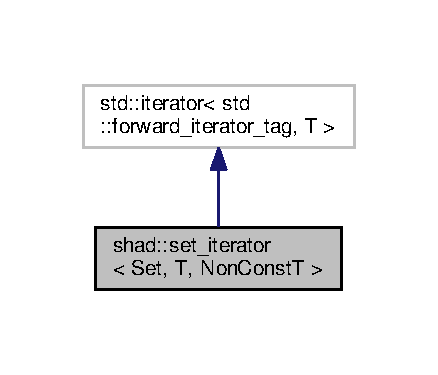
\includegraphics[width=210pt]{classshad_1_1set__iterator__inherit__graph}
\end{center}
\end{figure}


Collaboration diagram for shad\-:\-:set\-\_\-iterator$<$ Set, T, Non\-Const\-T $>$\-:
\nopagebreak
\begin{figure}[H]
\begin{center}
\leavevmode
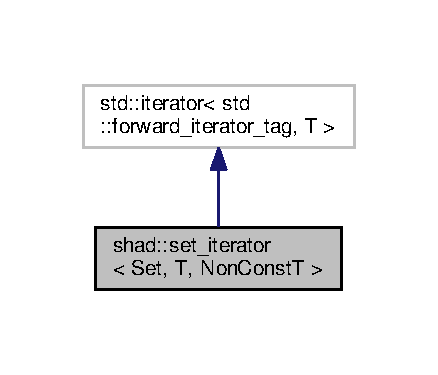
\includegraphics[width=210pt]{classshad_1_1set__iterator__coll__graph}
\end{center}
\end{figure}
\subsection*{Classes}
\begin{DoxyCompactItemize}
\item 
class \hyperlink{classshad_1_1set__iterator_1_1local__iterator__range}{local\-\_\-iterator\-\_\-range}
\end{DoxyCompactItemize}
\subsection*{Public Types}
\begin{DoxyCompactItemize}
\item 
using \hyperlink{classshad_1_1set__iterator_aa1c2447817e9c3156a213363f8914b29}{value\-\_\-type} = T
\item 
using \hyperlink{classshad_1_1set__iterator_a2da49754284fd7ddf591c2df4123b57d}{O\-I\-D\-T} = typename Set\-T\-::\-Object\-I\-D
\item 
using \hyperlink{classshad_1_1set__iterator_a526f8a1656d9a4826cf9d0ec1ab60ac6}{L\-Set} = typename Set\-T\-::\-L\-Set\-T
\item 
using \hyperlink{classshad_1_1set__iterator_a162b1b9d8dfe2e3a656fcdacf0450939}{local\-\_\-iterator\-\_\-type} = \hyperlink{classshad_1_1lset__iterator}{lset\-\_\-iterator}$<$ \hyperlink{classshad_1_1set__iterator_a526f8a1656d9a4826cf9d0ec1ab60ac6}{L\-Set}, T $>$
\end{DoxyCompactItemize}
\subsection*{Public Member Functions}
\begin{DoxyCompactItemize}
\item 
\hyperlink{classshad_1_1set__iterator_aaa748b984ba1889894b642048b4a0e19}{set\-\_\-iterator} ()
\item 
\hyperlink{classshad_1_1set__iterator_a48b9c19f645efb3625b552abd0970b13}{set\-\_\-iterator} (uint32\-\_\-t loc\-I\-D, const \hyperlink{classshad_1_1set__iterator_a2da49754284fd7ddf591c2df4123b57d}{O\-I\-D\-T} set\-O\-I\-D, \hyperlink{classshad_1_1set__iterator_a162b1b9d8dfe2e3a656fcdacf0450939}{local\-\_\-iterator\-\_\-type} \&lit, T element)
\item 
\hyperlink{classshad_1_1set__iterator_ac177dfe74c98af3943757273e499c8d5}{set\-\_\-iterator} (uint32\-\_\-t loc\-I\-D, const \hyperlink{classshad_1_1set__iterator_a2da49754284fd7ddf591c2df4123b57d}{O\-I\-D\-T} set\-O\-I\-D, \hyperlink{classshad_1_1set__iterator_a162b1b9d8dfe2e3a656fcdacf0450939}{local\-\_\-iterator\-\_\-type} \&lit)
\item 
bool \hyperlink{classshad_1_1set__iterator_af863b5f03ab32a49c8007e354a33cd38}{operator==} (const \hyperlink{classshad_1_1set__iterator}{set\-\_\-iterator} \&other) const 
\item 
bool \hyperlink{classshad_1_1set__iterator_ad31484cf73b92999b9d1b2979eef8046}{operator!=} (const \hyperlink{classshad_1_1set__iterator}{set\-\_\-iterator} \&other) const 
\item 
T \hyperlink{classshad_1_1set__iterator_a3ae23533d7aa28c234d61e7626f9e635}{operator$\ast$} () const 
\item 
\hyperlink{classshad_1_1set__iterator}{set\-\_\-iterator} \& \hyperlink{classshad_1_1set__iterator_ab1dc70400a6aac2e3fb89f0cbb7dee57}{operator++} ()
\item 
\hyperlink{classshad_1_1set__iterator}{set\-\_\-iterator} \hyperlink{classshad_1_1set__iterator_ad87b4d58f5c5febdc8ac4075df1b9781}{operator++} (int)
\end{DoxyCompactItemize}
\subsection*{Static Public Member Functions}
\begin{DoxyCompactItemize}
\item 
static \hyperlink{classshad_1_1set__iterator}{set\-\_\-iterator} \hyperlink{classshad_1_1set__iterator_a9dc1174f6bba2f83943450e0edcefdab}{set\-\_\-begin} (const Set\-T $\ast$set\-Ptr)
\item 
static \hyperlink{classshad_1_1set__iterator}{set\-\_\-iterator} \hyperlink{classshad_1_1set__iterator_a8985de6f91372745fd2a4686b6cdc2a9}{set\-\_\-end} (const Set\-T $\ast$set\-Ptr)
\item 
static \hyperlink{classshad_1_1set__iterator_1_1local__iterator__range}{local\-\_\-iterator\-\_\-range} \hyperlink{classshad_1_1set__iterator_a366136100eb4de6676eab9918c128483}{local\-\_\-range} (\hyperlink{classshad_1_1set__iterator}{set\-\_\-iterator} \&B, \hyperlink{classshad_1_1set__iterator}{set\-\_\-iterator} \&E)
\item 
static \hyperlink{classshad_1_1rt_1_1localities__range}{rt\-::localities\-\_\-range} \hyperlink{classshad_1_1set__iterator_a05e3dc79288b4f9dd03f9289612b22db}{localities} (\hyperlink{classshad_1_1set__iterator}{set\-\_\-iterator} \&B, \hyperlink{classshad_1_1set__iterator}{set\-\_\-iterator} \&E)
\item 
static \hyperlink{classshad_1_1set__iterator}{set\-\_\-iterator} \hyperlink{classshad_1_1set__iterator_a8c432b84360eae7b83eef48f8e96f417}{iterator\-\_\-from\-\_\-local} (\hyperlink{classshad_1_1set__iterator}{set\-\_\-iterator} \&B, \hyperlink{classshad_1_1set__iterator}{set\-\_\-iterator} \&E, \hyperlink{classshad_1_1set__iterator_a162b1b9d8dfe2e3a656fcdacf0450939}{local\-\_\-iterator\-\_\-type} itr)
\end{DoxyCompactItemize}


\subsection{Member Typedef Documentation}
\hypertarget{classshad_1_1set__iterator_a162b1b9d8dfe2e3a656fcdacf0450939}{\index{shad\-::set\-\_\-iterator@{shad\-::set\-\_\-iterator}!local\-\_\-iterator\-\_\-type@{local\-\_\-iterator\-\_\-type}}
\index{local\-\_\-iterator\-\_\-type@{local\-\_\-iterator\-\_\-type}!shad::set_iterator@{shad\-::set\-\_\-iterator}}
\subsubsection[{local\-\_\-iterator\-\_\-type}]{\setlength{\rightskip}{0pt plus 5cm}template$<$typename Set , typename T , typename Non\-Const\-T $>$ using {\bf shad\-::set\-\_\-iterator}$<$ {\bf Set}, T, Non\-Const\-T $>$\-::{\bf local\-\_\-iterator\-\_\-type} =  {\bf lset\-\_\-iterator}$<${\bf L\-Set}, T$>$}}\label{classshad_1_1set__iterator_a162b1b9d8dfe2e3a656fcdacf0450939}
\hypertarget{classshad_1_1set__iterator_a526f8a1656d9a4826cf9d0ec1ab60ac6}{\index{shad\-::set\-\_\-iterator@{shad\-::set\-\_\-iterator}!L\-Set@{L\-Set}}
\index{L\-Set@{L\-Set}!shad::set_iterator@{shad\-::set\-\_\-iterator}}
\subsubsection[{L\-Set}]{\setlength{\rightskip}{0pt plus 5cm}template$<$typename Set , typename T , typename Non\-Const\-T $>$ using {\bf shad\-::set\-\_\-iterator}$<$ {\bf Set}, T, Non\-Const\-T $>$\-::{\bf L\-Set} =  typename Set\-T\-::\-L\-Set\-T}}\label{classshad_1_1set__iterator_a526f8a1656d9a4826cf9d0ec1ab60ac6}
\hypertarget{classshad_1_1set__iterator_a2da49754284fd7ddf591c2df4123b57d}{\index{shad\-::set\-\_\-iterator@{shad\-::set\-\_\-iterator}!O\-I\-D\-T@{O\-I\-D\-T}}
\index{O\-I\-D\-T@{O\-I\-D\-T}!shad::set_iterator@{shad\-::set\-\_\-iterator}}
\subsubsection[{O\-I\-D\-T}]{\setlength{\rightskip}{0pt plus 5cm}template$<$typename Set , typename T , typename Non\-Const\-T $>$ using {\bf shad\-::set\-\_\-iterator}$<$ {\bf Set}, T, Non\-Const\-T $>$\-::{\bf O\-I\-D\-T} =  typename Set\-T\-::\-Object\-I\-D}}\label{classshad_1_1set__iterator_a2da49754284fd7ddf591c2df4123b57d}
\hypertarget{classshad_1_1set__iterator_aa1c2447817e9c3156a213363f8914b29}{\index{shad\-::set\-\_\-iterator@{shad\-::set\-\_\-iterator}!value\-\_\-type@{value\-\_\-type}}
\index{value\-\_\-type@{value\-\_\-type}!shad::set_iterator@{shad\-::set\-\_\-iterator}}
\subsubsection[{value\-\_\-type}]{\setlength{\rightskip}{0pt plus 5cm}template$<$typename Set , typename T , typename Non\-Const\-T $>$ using {\bf shad\-::set\-\_\-iterator}$<$ {\bf Set}, T, Non\-Const\-T $>$\-::{\bf value\-\_\-type} =  T}}\label{classshad_1_1set__iterator_aa1c2447817e9c3156a213363f8914b29}


\subsection{Constructor \& Destructor Documentation}
\hypertarget{classshad_1_1set__iterator_aaa748b984ba1889894b642048b4a0e19}{\index{shad\-::set\-\_\-iterator@{shad\-::set\-\_\-iterator}!set\-\_\-iterator@{set\-\_\-iterator}}
\index{set\-\_\-iterator@{set\-\_\-iterator}!shad::set_iterator@{shad\-::set\-\_\-iterator}}
\subsubsection[{set\-\_\-iterator}]{\setlength{\rightskip}{0pt plus 5cm}template$<$typename Set , typename T , typename Non\-Const\-T $>$ {\bf shad\-::set\-\_\-iterator}$<$ {\bf Set}, T, Non\-Const\-T $>$\-::{\bf set\-\_\-iterator} (
\begin{DoxyParamCaption}
{}
\end{DoxyParamCaption}
)\hspace{0.3cm}{\ttfamily [inline]}}}\label{classshad_1_1set__iterator_aaa748b984ba1889894b642048b4a0e19}
\hypertarget{classshad_1_1set__iterator_a48b9c19f645efb3625b552abd0970b13}{\index{shad\-::set\-\_\-iterator@{shad\-::set\-\_\-iterator}!set\-\_\-iterator@{set\-\_\-iterator}}
\index{set\-\_\-iterator@{set\-\_\-iterator}!shad::set_iterator@{shad\-::set\-\_\-iterator}}
\subsubsection[{set\-\_\-iterator}]{\setlength{\rightskip}{0pt plus 5cm}template$<$typename Set , typename T , typename Non\-Const\-T $>$ {\bf shad\-::set\-\_\-iterator}$<$ {\bf Set}, T, Non\-Const\-T $>$\-::{\bf set\-\_\-iterator} (
\begin{DoxyParamCaption}
\item[{uint32\-\_\-t}]{loc\-I\-D, }
\item[{const {\bf O\-I\-D\-T}}]{set\-O\-I\-D, }
\item[{{\bf local\-\_\-iterator\-\_\-type} \&}]{lit, }
\item[{T}]{element}
\end{DoxyParamCaption}
)\hspace{0.3cm}{\ttfamily [inline]}}}\label{classshad_1_1set__iterator_a48b9c19f645efb3625b552abd0970b13}
\hypertarget{classshad_1_1set__iterator_ac177dfe74c98af3943757273e499c8d5}{\index{shad\-::set\-\_\-iterator@{shad\-::set\-\_\-iterator}!set\-\_\-iterator@{set\-\_\-iterator}}
\index{set\-\_\-iterator@{set\-\_\-iterator}!shad::set_iterator@{shad\-::set\-\_\-iterator}}
\subsubsection[{set\-\_\-iterator}]{\setlength{\rightskip}{0pt plus 5cm}template$<$typename Set , typename T , typename Non\-Const\-T $>$ {\bf shad\-::set\-\_\-iterator}$<$ {\bf Set}, T, Non\-Const\-T $>$\-::{\bf set\-\_\-iterator} (
\begin{DoxyParamCaption}
\item[{uint32\-\_\-t}]{loc\-I\-D, }
\item[{const {\bf O\-I\-D\-T}}]{set\-O\-I\-D, }
\item[{{\bf local\-\_\-iterator\-\_\-type} \&}]{lit}
\end{DoxyParamCaption}
)\hspace{0.3cm}{\ttfamily [inline]}}}\label{classshad_1_1set__iterator_ac177dfe74c98af3943757273e499c8d5}


\subsection{Member Function Documentation}
\hypertarget{classshad_1_1set__iterator_a8c432b84360eae7b83eef48f8e96f417}{\index{shad\-::set\-\_\-iterator@{shad\-::set\-\_\-iterator}!iterator\-\_\-from\-\_\-local@{iterator\-\_\-from\-\_\-local}}
\index{iterator\-\_\-from\-\_\-local@{iterator\-\_\-from\-\_\-local}!shad::set_iterator@{shad\-::set\-\_\-iterator}}
\subsubsection[{iterator\-\_\-from\-\_\-local}]{\setlength{\rightskip}{0pt plus 5cm}template$<$typename Set , typename T , typename Non\-Const\-T $>$ static {\bf set\-\_\-iterator} {\bf shad\-::set\-\_\-iterator}$<$ {\bf Set}, T, Non\-Const\-T $>$\-::iterator\-\_\-from\-\_\-local (
\begin{DoxyParamCaption}
\item[{{\bf set\-\_\-iterator}$<$ {\bf Set}, T, Non\-Const\-T $>$ \&}]{B, }
\item[{{\bf set\-\_\-iterator}$<$ {\bf Set}, T, Non\-Const\-T $>$ \&}]{E, }
\item[{{\bf local\-\_\-iterator\-\_\-type}}]{itr}
\end{DoxyParamCaption}
)\hspace{0.3cm}{\ttfamily [inline]}, {\ttfamily [static]}}}\label{classshad_1_1set__iterator_a8c432b84360eae7b83eef48f8e96f417}
\hypertarget{classshad_1_1set__iterator_a366136100eb4de6676eab9918c128483}{\index{shad\-::set\-\_\-iterator@{shad\-::set\-\_\-iterator}!local\-\_\-range@{local\-\_\-range}}
\index{local\-\_\-range@{local\-\_\-range}!shad::set_iterator@{shad\-::set\-\_\-iterator}}
\subsubsection[{local\-\_\-range}]{\setlength{\rightskip}{0pt plus 5cm}template$<$typename Set , typename T , typename Non\-Const\-T $>$ static {\bf local\-\_\-iterator\-\_\-range} {\bf shad\-::set\-\_\-iterator}$<$ {\bf Set}, T, Non\-Const\-T $>$\-::local\-\_\-range (
\begin{DoxyParamCaption}
\item[{{\bf set\-\_\-iterator}$<$ {\bf Set}, T, Non\-Const\-T $>$ \&}]{B, }
\item[{{\bf set\-\_\-iterator}$<$ {\bf Set}, T, Non\-Const\-T $>$ \&}]{E}
\end{DoxyParamCaption}
)\hspace{0.3cm}{\ttfamily [inline]}, {\ttfamily [static]}}}\label{classshad_1_1set__iterator_a366136100eb4de6676eab9918c128483}
\hypertarget{classshad_1_1set__iterator_a05e3dc79288b4f9dd03f9289612b22db}{\index{shad\-::set\-\_\-iterator@{shad\-::set\-\_\-iterator}!localities@{localities}}
\index{localities@{localities}!shad::set_iterator@{shad\-::set\-\_\-iterator}}
\subsubsection[{localities}]{\setlength{\rightskip}{0pt plus 5cm}template$<$typename Set , typename T , typename Non\-Const\-T $>$ static {\bf rt\-::localities\-\_\-range} {\bf shad\-::set\-\_\-iterator}$<$ {\bf Set}, T, Non\-Const\-T $>$\-::localities (
\begin{DoxyParamCaption}
\item[{{\bf set\-\_\-iterator}$<$ {\bf Set}, T, Non\-Const\-T $>$ \&}]{B, }
\item[{{\bf set\-\_\-iterator}$<$ {\bf Set}, T, Non\-Const\-T $>$ \&}]{E}
\end{DoxyParamCaption}
)\hspace{0.3cm}{\ttfamily [inline]}, {\ttfamily [static]}}}\label{classshad_1_1set__iterator_a05e3dc79288b4f9dd03f9289612b22db}
\hypertarget{classshad_1_1set__iterator_ad31484cf73b92999b9d1b2979eef8046}{\index{shad\-::set\-\_\-iterator@{shad\-::set\-\_\-iterator}!operator!=@{operator!=}}
\index{operator!=@{operator!=}!shad::set_iterator@{shad\-::set\-\_\-iterator}}
\subsubsection[{operator!=}]{\setlength{\rightskip}{0pt plus 5cm}template$<$typename Set , typename T , typename Non\-Const\-T $>$ bool {\bf shad\-::set\-\_\-iterator}$<$ {\bf Set}, T, Non\-Const\-T $>$\-::operator!= (
\begin{DoxyParamCaption}
\item[{const {\bf set\-\_\-iterator}$<$ {\bf Set}, T, Non\-Const\-T $>$ \&}]{other}
\end{DoxyParamCaption}
) const\hspace{0.3cm}{\ttfamily [inline]}}}\label{classshad_1_1set__iterator_ad31484cf73b92999b9d1b2979eef8046}
\hypertarget{classshad_1_1set__iterator_a3ae23533d7aa28c234d61e7626f9e635}{\index{shad\-::set\-\_\-iterator@{shad\-::set\-\_\-iterator}!operator$\ast$@{operator$\ast$}}
\index{operator$\ast$@{operator$\ast$}!shad::set_iterator@{shad\-::set\-\_\-iterator}}
\subsubsection[{operator$\ast$}]{\setlength{\rightskip}{0pt plus 5cm}template$<$typename Set , typename T , typename Non\-Const\-T $>$ T {\bf shad\-::set\-\_\-iterator}$<$ {\bf Set}, T, Non\-Const\-T $>$\-::operator$\ast$ (
\begin{DoxyParamCaption}
{}
\end{DoxyParamCaption}
) const\hspace{0.3cm}{\ttfamily [inline]}}}\label{classshad_1_1set__iterator_a3ae23533d7aa28c234d61e7626f9e635}
\hypertarget{classshad_1_1set__iterator_ab1dc70400a6aac2e3fb89f0cbb7dee57}{\index{shad\-::set\-\_\-iterator@{shad\-::set\-\_\-iterator}!operator++@{operator++}}
\index{operator++@{operator++}!shad::set_iterator@{shad\-::set\-\_\-iterator}}
\subsubsection[{operator++}]{\setlength{\rightskip}{0pt plus 5cm}template$<$typename Set , typename T , typename Non\-Const\-T $>$ {\bf set\-\_\-iterator}\& {\bf shad\-::set\-\_\-iterator}$<$ {\bf Set}, T, Non\-Const\-T $>$\-::operator++ (
\begin{DoxyParamCaption}
{}
\end{DoxyParamCaption}
)\hspace{0.3cm}{\ttfamily [inline]}}}\label{classshad_1_1set__iterator_ab1dc70400a6aac2e3fb89f0cbb7dee57}
\hypertarget{classshad_1_1set__iterator_ad87b4d58f5c5febdc8ac4075df1b9781}{\index{shad\-::set\-\_\-iterator@{shad\-::set\-\_\-iterator}!operator++@{operator++}}
\index{operator++@{operator++}!shad::set_iterator@{shad\-::set\-\_\-iterator}}
\subsubsection[{operator++}]{\setlength{\rightskip}{0pt plus 5cm}template$<$typename Set , typename T , typename Non\-Const\-T $>$ {\bf set\-\_\-iterator} {\bf shad\-::set\-\_\-iterator}$<$ {\bf Set}, T, Non\-Const\-T $>$\-::operator++ (
\begin{DoxyParamCaption}
\item[{int}]{}
\end{DoxyParamCaption}
)\hspace{0.3cm}{\ttfamily [inline]}}}\label{classshad_1_1set__iterator_ad87b4d58f5c5febdc8ac4075df1b9781}
\hypertarget{classshad_1_1set__iterator_af863b5f03ab32a49c8007e354a33cd38}{\index{shad\-::set\-\_\-iterator@{shad\-::set\-\_\-iterator}!operator==@{operator==}}
\index{operator==@{operator==}!shad::set_iterator@{shad\-::set\-\_\-iterator}}
\subsubsection[{operator==}]{\setlength{\rightskip}{0pt plus 5cm}template$<$typename Set , typename T , typename Non\-Const\-T $>$ bool {\bf shad\-::set\-\_\-iterator}$<$ {\bf Set}, T, Non\-Const\-T $>$\-::operator== (
\begin{DoxyParamCaption}
\item[{const {\bf set\-\_\-iterator}$<$ {\bf Set}, T, Non\-Const\-T $>$ \&}]{other}
\end{DoxyParamCaption}
) const\hspace{0.3cm}{\ttfamily [inline]}}}\label{classshad_1_1set__iterator_af863b5f03ab32a49c8007e354a33cd38}
\hypertarget{classshad_1_1set__iterator_a9dc1174f6bba2f83943450e0edcefdab}{\index{shad\-::set\-\_\-iterator@{shad\-::set\-\_\-iterator}!set\-\_\-begin@{set\-\_\-begin}}
\index{set\-\_\-begin@{set\-\_\-begin}!shad::set_iterator@{shad\-::set\-\_\-iterator}}
\subsubsection[{set\-\_\-begin}]{\setlength{\rightskip}{0pt plus 5cm}template$<$typename Set , typename T , typename Non\-Const\-T $>$ static {\bf set\-\_\-iterator} {\bf shad\-::set\-\_\-iterator}$<$ {\bf Set}, T, Non\-Const\-T $>$\-::set\-\_\-begin (
\begin{DoxyParamCaption}
\item[{const Set\-T $\ast$}]{set\-Ptr}
\end{DoxyParamCaption}
)\hspace{0.3cm}{\ttfamily [inline]}, {\ttfamily [static]}}}\label{classshad_1_1set__iterator_a9dc1174f6bba2f83943450e0edcefdab}
\hypertarget{classshad_1_1set__iterator_a8985de6f91372745fd2a4686b6cdc2a9}{\index{shad\-::set\-\_\-iterator@{shad\-::set\-\_\-iterator}!set\-\_\-end@{set\-\_\-end}}
\index{set\-\_\-end@{set\-\_\-end}!shad::set_iterator@{shad\-::set\-\_\-iterator}}
\subsubsection[{set\-\_\-end}]{\setlength{\rightskip}{0pt plus 5cm}template$<$typename Set , typename T , typename Non\-Const\-T $>$ static {\bf set\-\_\-iterator} {\bf shad\-::set\-\_\-iterator}$<$ {\bf Set}, T, Non\-Const\-T $>$\-::set\-\_\-end (
\begin{DoxyParamCaption}
\item[{const Set\-T $\ast$}]{set\-Ptr}
\end{DoxyParamCaption}
)\hspace{0.3cm}{\ttfamily [inline]}, {\ttfamily [static]}}}\label{classshad_1_1set__iterator_a8985de6f91372745fd2a4686b6cdc2a9}


The documentation for this class was generated from the following file\-:\begin{DoxyCompactItemize}
\item 
include/shad/data\-\_\-structures/\hyperlink{set_8h}{set.\-h}\end{DoxyCompactItemize}

\hypertarget{classshad_1_1unordered__map}{\section{shad\-:\-:unordered\-\_\-map$<$ Key, T, Hash $>$ Class Template Reference}
\label{classshad_1_1unordered__map}\index{shad\-::unordered\-\_\-map$<$ Key, T, Hash $>$@{shad\-::unordered\-\_\-map$<$ Key, T, Hash $>$}}
}


Distributed unordered associative map.  




{\ttfamily \#include $<$shad/core/unordered\-\_\-map.\-h$>$}

\subsection*{Public Types}
\begin{DoxyCompactItemize}
\item 
using \hyperlink{group__Types_gac2a5bb16d47a5da2d493616e6fa5a73c}{key\-\_\-type} = Key
\item 
using \hyperlink{group__Types_ga146f53b5d4191c21deed1bd89683d4bf}{mapped\-\_\-type} = T
\begin{DoxyCompactList}\small\item\em The type of the mapped elements. \end{DoxyCompactList}\item 
using \hyperlink{group__Types_ga930e4848d41a2efe4d2e47f52650a76c}{value\-\_\-type} = typename \hyperlink{classshad_1_1Hashmap_ad8c0108347b59bcd19ccb8070a313dd8}{hashmap\-\_\-t\-::value\-\_\-type}
\begin{DoxyCompactList}\small\item\em The type of the stored value. \end{DoxyCompactList}\item 
using \hyperlink{group__Types_ga2a84980e6d435a8a7b1a99f78b828a65}{size\-\_\-type} = std\-::size\-\_\-t
\begin{DoxyCompactList}\small\item\em The type used to represent size. \end{DoxyCompactList}\item 
using \hyperlink{group__Types_ga2a1294efcd043aa4bbb5da7c3c811448}{difference\-\_\-type} = std\-::ptrdiff\-\_\-t
\begin{DoxyCompactList}\small\item\em The type used to represent distances. \end{DoxyCompactList}\item 
using \hyperlink{group__Types_ga94466a187a2da262cb5b58356c3ac24c}{pointer} = \hyperlink{group__Types_ga930e4848d41a2efe4d2e47f52650a76c}{value\-\_\-type} $\ast$
\begin{DoxyCompactList}\small\item\em The type for pointer to \-::value\-\_\-type. \end{DoxyCompactList}\item 
using \hyperlink{group__Types_ga4db9d56c27ddb72ccad61249ef55c54c}{const\-\_\-pointer} = const \hyperlink{group__Types_ga930e4848d41a2efe4d2e47f52650a76c}{value\-\_\-type} $\ast$
\begin{DoxyCompactList}\small\item\em The type for pointer to \-::const\-\_\-value\-\_\-type. \end{DoxyCompactList}\item 
using \hyperlink{group__Types_gab52d604c26835c20a0363f9affa7ff57}{iterator} = typename \hyperlink{classshad_1_1Hashmap_a4603e48d3ad3a380abc888671e55bf01}{hashmap\-\_\-t\-::iterator}
\begin{DoxyCompactList}\small\item\em The type of iterators on the map. \end{DoxyCompactList}\item 
using \hyperlink{group__Types_ga102c3cd521767bf4b22f3788ccc054e8}{const\-\_\-iterator} = typename \hyperlink{classshad_1_1Hashmap_a1f8a379c42bc2d4b67dcc9f519dc537e}{hashmap\-\_\-t\-::const\-\_\-iterator}
\begin{DoxyCompactList}\small\item\em The type of const iterators on the map. \end{DoxyCompactList}\item 
using \hyperlink{group__Types_ga520d395c30b2b19179153108ea694cec}{local\-\_\-iterator} = typename \hyperlink{classshad_1_1Hashmap_abf95d16be9ba9060bff9fa591ece302f}{hashmap\-\_\-t\-::local\-\_\-iterator}
\begin{DoxyCompactList}\small\item\em The type of local iterators on the map. \end{DoxyCompactList}\item 
using \hyperlink{group__Types_ga2242fb2071462a5f8a420d8cd8a7d8e8}{const\-\_\-local\-\_\-iterator} = typename \hyperlink{classshad_1_1Hashmap_afdf2dad495223a7d8bcec4256b591d89}{hashmap\-\_\-t\-::const\-\_\-local\-\_\-iterator}
\begin{DoxyCompactList}\small\item\em The type of const local iterators on the map. \end{DoxyCompactList}\end{DoxyCompactItemize}
\subsection*{Public Member Functions}
\begin{DoxyCompactItemize}
\item 
\hyperlink{classshad_1_1unordered__map_acd64334034dd1af3a1cc39f3b62fc622}{unordered\-\_\-map} (\hyperlink{group__Types_ga2a84980e6d435a8a7b1a99f78b828a65}{size\-\_\-type} bucket\-\_\-count=1021, const Hash \&\hyperlink{structshad_1_1hash}{hash}=Hash())
\begin{DoxyCompactList}\small\item\em Constructor. \end{DoxyCompactList}\item 
\hyperlink{classshad_1_1unordered__map_a3964d9033e56109fbbcabdf565c2d8a9}{$\sim$unordered\-\_\-map} ()
\begin{DoxyCompactList}\small\item\em Destructor. \end{DoxyCompactList}\item 
constexpr \hyperlink{group__Types_gab52d604c26835c20a0363f9affa7ff57}{iterator} \hyperlink{group__Iterators_ga3753eddf67b531a3718ae7eb1e33b131}{begin} () const noexcept
\item 
constexpr \hyperlink{group__Types_ga102c3cd521767bf4b22f3788ccc054e8}{const\-\_\-iterator} \hyperlink{group__Iterators_gaf264a3126cd78a96da927c0f17890fca}{cbegin} () const noexcept
\begin{DoxyCompactList}\small\item\em The iterator to the beginning of the sequence. \end{DoxyCompactList}\item 
constexpr \hyperlink{group__Types_gab52d604c26835c20a0363f9affa7ff57}{iterator} \hyperlink{group__Iterators_ga5a1c3f388ffec559f61de7e2eb17eaa2}{end} () const noexcept
\begin{DoxyCompactList}\small\item\em The iterator to the end of the sequence. \end{DoxyCompactList}\item 
constexpr \hyperlink{group__Types_ga102c3cd521767bf4b22f3788ccc054e8}{const\-\_\-iterator} \hyperlink{group__Iterators_ga563bf6f0949e2ed31c86fc2b22f26df1}{cend} () const noexcept
\begin{DoxyCompactList}\small\item\em The iterator to the end of the sequence. \end{DoxyCompactList}\item 
bool \hyperlink{group__Capacity_gade6abbe1bedf25b8c2fb53eab2420e71}{empty} () const noexcept
\item 
\hyperlink{group__Types_ga2a84980e6d435a8a7b1a99f78b828a65}{size\-\_\-type} \hyperlink{group__Capacity_ga0d8b21fa4842806604fa7a5f82d6f637}{size} () const noexcept
\begin{DoxyCompactList}\small\item\em The size of the container. \end{DoxyCompactList}\end{DoxyCompactItemize}
\subsection*{Friends}
\begin{DoxyCompactItemize}
\item 
class \hyperlink{classshad_1_1unordered__map_a178983bb5902294d2c70ed8b802b4a03}{buffered\-\_\-insert\-\_\-iterator$<$ unordered\-\_\-map $>$}
\end{DoxyCompactItemize}


\subsection{Detailed Description}
\subsubsection*{template$<$class Key, class T, class Hash = shad\-::hash$<$\-Key$>$$>$class shad\-::unordered\-\_\-map$<$ Key, T, Hash $>$}

Distributed unordered associative map. 

A distributed associative container that contains key-\/value pairs with unique keys. Search, insertion, and removal of elements have average constant-\/time complexity. Internally, the elements are not sorted in any particular order, but organized into buckets. Which bucket an element is placed into depends entirely on the hash of its key. This allows fast access to individual elements, since once the hash is computed, it refers to the exact bucket the element is placed into.


\begin{DoxyTemplParams}{Template Parameters}
{\em Key} & The type of the keys. \\
\hline
{\em T} & The type of the mapped values. \\
\hline
{\em Hash} & The type of the hashing callable.\\
\hline
\end{DoxyTemplParams}
\begin{DoxyRefDesc}{Todo}
\item[\hyperlink{todo__todo000001}{Todo}]Key\-Equal template parameter 

Allocator template parameter \end{DoxyRefDesc}


\subsection{Constructor \& Destructor Documentation}
\hypertarget{classshad_1_1unordered__map_acd64334034dd1af3a1cc39f3b62fc622}{\index{shad\-::unordered\-\_\-map@{shad\-::unordered\-\_\-map}!unordered\-\_\-map@{unordered\-\_\-map}}
\index{unordered\-\_\-map@{unordered\-\_\-map}!shad::unordered_map@{shad\-::unordered\-\_\-map}}
\subsubsection[{unordered\-\_\-map}]{\setlength{\rightskip}{0pt plus 5cm}template$<$class Key , class T , class Hash  = shad\-::hash$<$\-Key$>$$>$ {\bf shad\-::unordered\-\_\-map}$<$ Key, T, Hash $>$\-::{\bf unordered\-\_\-map} (
\begin{DoxyParamCaption}
\item[{{\bf size\-\_\-type}}]{bucket\-\_\-count = {\ttfamily 1021}, }
\item[{const Hash \&}]{hash = {\ttfamily Hash()}}
\end{DoxyParamCaption}
)\hspace{0.3cm}{\ttfamily [inline]}, {\ttfamily [explicit]}}}\label{classshad_1_1unordered__map_acd64334034dd1af3a1cc39f3b62fc622}


Constructor. 


\begin{DoxyParams}{Parameters}
{\em bucket\-\_\-count} & The minimum number of buckets. \\
\hline
{\em hash} & The hashing callable.\\
\hline
\end{DoxyParams}
\begin{DoxyRefDesc}{Todo}
\item[\hyperlink{todo__todo000002}{Todo}]add equal parameter 

add allocator parameter \end{DoxyRefDesc}
\hypertarget{classshad_1_1unordered__map_a3964d9033e56109fbbcabdf565c2d8a9}{\index{shad\-::unordered\-\_\-map@{shad\-::unordered\-\_\-map}!$\sim$unordered\-\_\-map@{$\sim$unordered\-\_\-map}}
\index{$\sim$unordered\-\_\-map@{$\sim$unordered\-\_\-map}!shad::unordered_map@{shad\-::unordered\-\_\-map}}
\subsubsection[{$\sim$unordered\-\_\-map}]{\setlength{\rightskip}{0pt plus 5cm}template$<$class Key , class T , class Hash  = shad\-::hash$<$\-Key$>$$>$ {\bf shad\-::unordered\-\_\-map}$<$ Key, T, Hash $>$\-::$\sim${\bf unordered\-\_\-map} (
\begin{DoxyParamCaption}
{}
\end{DoxyParamCaption}
)\hspace{0.3cm}{\ttfamily [inline]}}}\label{classshad_1_1unordered__map_a3964d9033e56109fbbcabdf565c2d8a9}


Destructor. 



\subsection{Friends And Related Function Documentation}
\hypertarget{classshad_1_1unordered__map_a178983bb5902294d2c70ed8b802b4a03}{\index{shad\-::unordered\-\_\-map@{shad\-::unordered\-\_\-map}!buffered\-\_\-insert\-\_\-iterator$<$ unordered\-\_\-map $>$@{buffered\-\_\-insert\-\_\-iterator$<$ unordered\-\_\-map $>$}}
\index{buffered\-\_\-insert\-\_\-iterator$<$ unordered\-\_\-map $>$@{buffered\-\_\-insert\-\_\-iterator$<$ unordered\-\_\-map $>$}!shad::unordered_map@{shad\-::unordered\-\_\-map}}
\subsubsection[{buffered\-\_\-insert\-\_\-iterator$<$ unordered\-\_\-map $>$}]{\setlength{\rightskip}{0pt plus 5cm}template$<$class Key , class T , class Hash  = shad\-::hash$<$\-Key$>$$>$ friend class {\bf buffered\-\_\-insert\-\_\-iterator}$<$ {\bf unordered\-\_\-map} $>$\hspace{0.3cm}{\ttfamily [friend]}}}\label{classshad_1_1unordered__map_a178983bb5902294d2c70ed8b802b4a03}


The documentation for this class was generated from the following file\-:\begin{DoxyCompactItemize}
\item 
include/shad/core/\hyperlink{unordered__map_8h}{unordered\-\_\-map.\-h}\end{DoxyCompactItemize}

\hypertarget{classshad_1_1unordered__set}{\section{shad\-:\-:unordered\-\_\-set$<$ Key, Hash $>$ Class Template Reference}
\label{classshad_1_1unordered__set}\index{shad\-::unordered\-\_\-set$<$ Key, Hash $>$@{shad\-::unordered\-\_\-set$<$ Key, Hash $>$}}
}


Distributed unordered set.  




{\ttfamily \#include $<$shad/core/unordered\-\_\-set.\-h$>$}

\subsection*{Public Types}
\begin{DoxyCompactItemize}
\item 
using \hyperlink{group__Types_gae860c65ed861f8aa69b0360638f4ad5d}{key\-\_\-type} = Key
\item 
using \hyperlink{group__Types_ga56832ea0d8218bf22f59a2e8ff4de499}{value\-\_\-type} = typename \hyperlink{classshad_1_1Set_a20c26f02edb7c6c978a0e0b6f2b46c80}{set\-\_\-t\-::value\-\_\-type}
\begin{DoxyCompactList}\small\item\em The type of the stored value. \end{DoxyCompactList}\item 
using \hyperlink{group__Types_gaf733341726e3097cf440257afa76d76a}{size\-\_\-type} = std\-::size\-\_\-t
\begin{DoxyCompactList}\small\item\em The type used to represent size. \end{DoxyCompactList}\item 
using \hyperlink{group__Types_gaa58125290d23043a3bdfa2430291a1e8}{difference\-\_\-type} = std\-::ptrdiff\-\_\-t
\begin{DoxyCompactList}\small\item\em The type used to represent distances. \end{DoxyCompactList}\item 
using \hyperlink{group__Types_ga84503e3a7375cd54f32da739fe21ecc9}{pointer} = \hyperlink{group__Types_ga56832ea0d8218bf22f59a2e8ff4de499}{value\-\_\-type} $\ast$
\begin{DoxyCompactList}\small\item\em The type for pointer to \-::value\-\_\-type. \end{DoxyCompactList}\item 
using \hyperlink{group__Types_ga3d079442c0e215d47f0c93f05b2ddb1f}{const\-\_\-pointer} = const \hyperlink{group__Types_ga56832ea0d8218bf22f59a2e8ff4de499}{value\-\_\-type} $\ast$
\begin{DoxyCompactList}\small\item\em The type for pointer to \-::const\-\_\-value\-\_\-type. \end{DoxyCompactList}\item 
using \hyperlink{group__Types_gadbad50ac069a38bd820c0a9f532f903e}{iterator} = typename \hyperlink{classshad_1_1Set_a726ddfe3c1c55db2ef60c5c1960d6666}{set\-\_\-t\-::iterator}
\begin{DoxyCompactList}\small\item\em The type of iterators on the set. \end{DoxyCompactList}\item 
using \hyperlink{group__Types_ga074f67d0516c3a68d8c79976aef62fb1}{const\-\_\-iterator} = typename \hyperlink{classshad_1_1Set_a0b2608f92f5397a25e62fad925fc177e}{set\-\_\-t\-::const\-\_\-iterator}
\begin{DoxyCompactList}\small\item\em The type of const iterators on the set. \end{DoxyCompactList}\item 
using \hyperlink{group__Types_gae1ee2e5ce1b39afa3cb1ce248747324d}{local\-\_\-iterator} = typename \hyperlink{classshad_1_1Set_a12ce7d6fd8fd0569035b0eb236b22179}{set\-\_\-t\-::local\-\_\-iterator}
\begin{DoxyCompactList}\small\item\em The type of local iterators on the set. \end{DoxyCompactList}\item 
using \hyperlink{group__Types_gac14878d16fabddc52f8dd35465f3155e}{const\-\_\-local\-\_\-iterator} = typename \hyperlink{classshad_1_1Set_a0857d9ce7a249e860e3a67bc18f7de8b}{set\-\_\-t\-::const\-\_\-local\-\_\-iterator}
\begin{DoxyCompactList}\small\item\em The type of const local iterators on the set. \end{DoxyCompactList}\end{DoxyCompactItemize}
\subsection*{Public Member Functions}
\begin{DoxyCompactItemize}
\item 
\hyperlink{classshad_1_1unordered__set_a05537f8a3c0c08af1910e2780b113f32}{unordered\-\_\-set} (\hyperlink{group__Types_gaf733341726e3097cf440257afa76d76a}{size\-\_\-type} bucket\-\_\-count=1021, const Hash \&\hyperlink{structshad_1_1hash}{hash}=Hash())
\begin{DoxyCompactList}\small\item\em Constructor. \end{DoxyCompactList}\item 
\hyperlink{classshad_1_1unordered__set_aa85876afdf2158838521bcaf4b270fa7}{$\sim$unordered\-\_\-set} ()
\begin{DoxyCompactList}\small\item\em Destructor. \end{DoxyCompactList}\item 
constexpr \hyperlink{group__Types_gadbad50ac069a38bd820c0a9f532f903e}{iterator} \hyperlink{group__Iterators_gaed1fcf07d265d37157a2bd2614b32693}{begin} () const noexcept
\item 
constexpr \hyperlink{group__Types_ga074f67d0516c3a68d8c79976aef62fb1}{const\-\_\-iterator} \hyperlink{group__Iterators_ga4317481540662a5afe3078e89b8012dd}{cbegin} () const noexcept
\begin{DoxyCompactList}\small\item\em The iterator to the beginning of the sequence. \end{DoxyCompactList}\item 
constexpr \hyperlink{group__Types_gadbad50ac069a38bd820c0a9f532f903e}{iterator} \hyperlink{group__Iterators_ga8ef3a0bbbef71c5658dbb7d6bd9751e9}{end} () const noexcept
\begin{DoxyCompactList}\small\item\em The iterator to the end of the sequence. \end{DoxyCompactList}\item 
constexpr \hyperlink{group__Types_ga074f67d0516c3a68d8c79976aef62fb1}{const\-\_\-iterator} \hyperlink{group__Iterators_ga5be7a60951a7f054b7770b385e370840}{cend} () const noexcept
\begin{DoxyCompactList}\small\item\em The iterator to the end of the sequence. \end{DoxyCompactList}\item 
bool \hyperlink{group__Capacity_gaa881674aa4274da05c2389348d09bbd3}{empty} () const noexcept
\item 
\hyperlink{group__Types_gaf733341726e3097cf440257afa76d76a}{size\-\_\-type} \hyperlink{group__Capacity_ga2586e3957d1c48a278edaaa1be72f92b}{size} () const noexcept
\begin{DoxyCompactList}\small\item\em The size of the container. \end{DoxyCompactList}\end{DoxyCompactItemize}
\subsection*{Friends}
\begin{DoxyCompactItemize}
\item 
class \hyperlink{classshad_1_1unordered__set_a37f994eeafee71345ca4e4e8cd1435e8}{buffered\-\_\-insert\-\_\-iterator$<$ unordered\-\_\-set $>$}
\end{DoxyCompactItemize}


\subsection{Detailed Description}
\subsubsection*{template$<$class Key, class Hash = shad\-::hash$<$\-Key$>$$>$class shad\-::unordered\-\_\-set$<$ Key, Hash $>$}

Distributed unordered set. 

A distributed associative container that contains a set of unique objects of type Key. Search, insertion, and removal have average constant-\/time complexity. Internally, the elements are not sorted in any particular order, but organized into buckets. Which bucket an element is placed into depends entirely on the hash of its value. This allows fast access to individual elements, since once a hash is computed, it refers to the exact bucket the element is placed into.


\begin{DoxyTemplParams}{Template Parameters}
{\em Key} & The type of the elements. \\
\hline
{\em Hash} & The type of the hashing callable.\\
\hline
\end{DoxyTemplParams}
\begin{DoxyRefDesc}{Todo}
\item[\hyperlink{todo__todo000003}{Todo}]Key\-Equal template parameter 

Allocator template parameter \end{DoxyRefDesc}


\subsection{Constructor \& Destructor Documentation}
\hypertarget{classshad_1_1unordered__set_a05537f8a3c0c08af1910e2780b113f32}{\index{shad\-::unordered\-\_\-set@{shad\-::unordered\-\_\-set}!unordered\-\_\-set@{unordered\-\_\-set}}
\index{unordered\-\_\-set@{unordered\-\_\-set}!shad::unordered_set@{shad\-::unordered\-\_\-set}}
\subsubsection[{unordered\-\_\-set}]{\setlength{\rightskip}{0pt plus 5cm}template$<$class Key , class Hash  = shad\-::hash$<$\-Key$>$$>$ {\bf shad\-::unordered\-\_\-set}$<$ Key, Hash $>$\-::{\bf unordered\-\_\-set} (
\begin{DoxyParamCaption}
\item[{{\bf size\-\_\-type}}]{bucket\-\_\-count = {\ttfamily 1021}, }
\item[{const Hash \&}]{hash = {\ttfamily Hash()}}
\end{DoxyParamCaption}
)\hspace{0.3cm}{\ttfamily [inline]}, {\ttfamily [explicit]}}}\label{classshad_1_1unordered__set_a05537f8a3c0c08af1910e2780b113f32}


Constructor. 


\begin{DoxyParams}{Parameters}
{\em bucket\-\_\-count} & The minimum number of buckets. \\
\hline
{\em hash} & The hashing callable.\\
\hline
\end{DoxyParams}
\begin{DoxyRefDesc}{Todo}
\item[\hyperlink{todo__todo000004}{Todo}]add equal parameter 

add allocator parameter \end{DoxyRefDesc}
\hypertarget{classshad_1_1unordered__set_aa85876afdf2158838521bcaf4b270fa7}{\index{shad\-::unordered\-\_\-set@{shad\-::unordered\-\_\-set}!$\sim$unordered\-\_\-set@{$\sim$unordered\-\_\-set}}
\index{$\sim$unordered\-\_\-set@{$\sim$unordered\-\_\-set}!shad::unordered_set@{shad\-::unordered\-\_\-set}}
\subsubsection[{$\sim$unordered\-\_\-set}]{\setlength{\rightskip}{0pt plus 5cm}template$<$class Key , class Hash  = shad\-::hash$<$\-Key$>$$>$ {\bf shad\-::unordered\-\_\-set}$<$ Key, Hash $>$\-::$\sim${\bf unordered\-\_\-set} (
\begin{DoxyParamCaption}
{}
\end{DoxyParamCaption}
)\hspace{0.3cm}{\ttfamily [inline]}}}\label{classshad_1_1unordered__set_aa85876afdf2158838521bcaf4b270fa7}


Destructor. 



\subsection{Friends And Related Function Documentation}
\hypertarget{classshad_1_1unordered__set_a37f994eeafee71345ca4e4e8cd1435e8}{\index{shad\-::unordered\-\_\-set@{shad\-::unordered\-\_\-set}!buffered\-\_\-insert\-\_\-iterator$<$ unordered\-\_\-set $>$@{buffered\-\_\-insert\-\_\-iterator$<$ unordered\-\_\-set $>$}}
\index{buffered\-\_\-insert\-\_\-iterator$<$ unordered\-\_\-set $>$@{buffered\-\_\-insert\-\_\-iterator$<$ unordered\-\_\-set $>$}!shad::unordered_set@{shad\-::unordered\-\_\-set}}
\subsubsection[{buffered\-\_\-insert\-\_\-iterator$<$ unordered\-\_\-set $>$}]{\setlength{\rightskip}{0pt plus 5cm}template$<$class Key , class Hash  = shad\-::hash$<$\-Key$>$$>$ friend class {\bf buffered\-\_\-insert\-\_\-iterator}$<$ {\bf unordered\-\_\-set} $>$\hspace{0.3cm}{\ttfamily [friend]}}}\label{classshad_1_1unordered__set_a37f994eeafee71345ca4e4e8cd1435e8}


The documentation for this class was generated from the following file\-:\begin{DoxyCompactItemize}
\item 
include/shad/core/\hyperlink{unordered__set_8h}{unordered\-\_\-set.\-h}\end{DoxyCompactItemize}

\hypertarget{structshad_1_1Updater}{\section{shad\-:\-:Updater$<$ T $>$ Struct Template Reference}
\label{structshad_1_1Updater}\index{shad\-::\-Updater$<$ T $>$@{shad\-::\-Updater$<$ T $>$}}
}


{\ttfamily \#include $<$shad/data\-\_\-structures/local\-\_\-hashmap.\-h$>$}

\subsection*{Public Member Functions}
\begin{DoxyCompactItemize}
\item 
bool \hyperlink{structshad_1_1Updater_a5edad1e56b0b35ed884e3d744e1e47e8}{operator()} (T $\ast$const lhs, const T \&rhs, bool same\-\_\-key)
\end{DoxyCompactItemize}
\subsection*{Static Public Member Functions}
\begin{DoxyCompactItemize}
\item 
static bool \hyperlink{structshad_1_1Updater_ae11f09a8191c7018a2115fe5a96f8b50}{Insert} (T $\ast$const lhs, const T \&rhs, bool same\-\_\-key)
\end{DoxyCompactItemize}


\subsection{Member Function Documentation}
\hypertarget{structshad_1_1Updater_ae11f09a8191c7018a2115fe5a96f8b50}{\index{shad\-::\-Updater@{shad\-::\-Updater}!Insert@{Insert}}
\index{Insert@{Insert}!shad::Updater@{shad\-::\-Updater}}
\subsubsection[{Insert}]{\setlength{\rightskip}{0pt plus 5cm}template$<$typename T $>$ static bool {\bf shad\-::\-Updater}$<$ T $>$\-::Insert (
\begin{DoxyParamCaption}
\item[{T $\ast$const}]{lhs, }
\item[{const T \&}]{rhs, }
\item[{bool}]{same\-\_\-key}
\end{DoxyParamCaption}
)\hspace{0.3cm}{\ttfamily [inline]}, {\ttfamily [static]}}}\label{structshad_1_1Updater_ae11f09a8191c7018a2115fe5a96f8b50}
\hypertarget{structshad_1_1Updater_a5edad1e56b0b35ed884e3d744e1e47e8}{\index{shad\-::\-Updater@{shad\-::\-Updater}!operator()@{operator()}}
\index{operator()@{operator()}!shad::Updater@{shad\-::\-Updater}}
\subsubsection[{operator()}]{\setlength{\rightskip}{0pt plus 5cm}template$<$typename T $>$ bool {\bf shad\-::\-Updater}$<$ T $>$\-::operator() (
\begin{DoxyParamCaption}
\item[{T $\ast$const}]{lhs, }
\item[{const T \&}]{rhs, }
\item[{bool}]{same\-\_\-key}
\end{DoxyParamCaption}
)\hspace{0.3cm}{\ttfamily [inline]}}}\label{structshad_1_1Updater_a5edad1e56b0b35ed884e3d744e1e47e8}


The documentation for this struct was generated from the following file\-:\begin{DoxyCompactItemize}
\item 
include/shad/data\-\_\-structures/\hyperlink{local__hashmap_8h}{local\-\_\-hashmap.\-h}\end{DoxyCompactItemize}

\hypertarget{classshad_1_1Vector}{\section{shad\-:\-:Vector$<$ T, Allocator $>$ Class Template Reference}
\label{classshad_1_1Vector}\index{shad\-::\-Vector$<$ T, Allocator $>$@{shad\-::\-Vector$<$ T, Allocator $>$}}
}


The \hyperlink{classshad_1_1Vector}{Vector} data Structure.  




{\ttfamily \#include $<$shad/data\-\_\-structures/vector.\-h$>$}



Inheritance diagram for shad\-:\-:Vector$<$ T, Allocator $>$\-:
\nopagebreak
\begin{figure}[H]
\begin{center}
\leavevmode
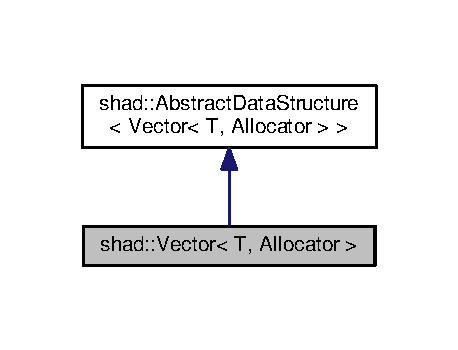
\includegraphics[width=220pt]{classshad_1_1Vector__inherit__graph}
\end{center}
\end{figure}


Collaboration diagram for shad\-:\-:Vector$<$ T, Allocator $>$\-:
\nopagebreak
\begin{figure}[H]
\begin{center}
\leavevmode
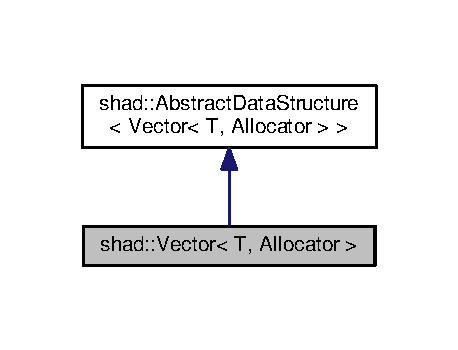
\includegraphics[width=220pt]{classshad_1_1Vector__coll__graph}
\end{center}
\end{figure}
\subsection*{Public Types}
\begin{DoxyCompactItemize}
\item 
using \hyperlink{classshad_1_1Vector_ad950d846edeeed7cc4a9163f9f679624}{allocator\-\_\-type} = Allocator
\begin{DoxyCompactList}\small\item\em The type of the allocator. \end{DoxyCompactList}\item 
using \hyperlink{classshad_1_1Vector_adb97b89826617473f44b4bb1dd3308ba}{value\-\_\-type} = T
\begin{DoxyCompactList}\small\item\em The type of the elements stored in the \hyperlink{classshad_1_1Vector}{shad\-::\-Vector}. \end{DoxyCompactList}\item 
using \hyperlink{classshad_1_1Vector_a46e5348988a063d58ed55c76fc94cec1}{difference\-\_\-type} = typename allocator\-\_\-type\-::difference\-\_\-type
\begin{DoxyCompactList}\small\item\em A signed integral type used the difference between iterators. \end{DoxyCompactList}\item 
using \hyperlink{classshad_1_1Vector_a1c97f4eb87d738cb4de97e5b3587c397}{size\-\_\-type} = typename allocator\-\_\-type\-::size\-\_\-type
\begin{DoxyCompactList}\small\item\em An unsigned integral type that can represent any non-\/negative value of difference\-\_\-type. \end{DoxyCompactList}\item 
using \hyperlink{classshad_1_1Vector_aaa71fd41daa1548f8436bc54ef507976}{iterator} = Iterator$<$ T $>$
\begin{DoxyCompactList}\small\item\em A random access iterator to \hyperlink{classshad_1_1Vector_adb97b89826617473f44b4bb1dd3308ba}{shad\-::\-Vector\-::value\-\_\-type}. \end{DoxyCompactList}\item 
using \hyperlink{classshad_1_1Vector_ab677e6f62431a450c856e7ffe44efbc6}{const\-\_\-iterator} = Iterator$<$ const T $>$
\begin{DoxyCompactList}\small\item\em A random access iterator to const \hyperlink{classshad_1_1Vector_adb97b89826617473f44b4bb1dd3308ba}{shad\-::\-Vector\-::value\-\_\-type}. \end{DoxyCompactList}\item 
using \hyperlink{classshad_1_1Vector_a71193856f7dddb5e9fe0128fe5d12448}{Object\-I\-D} = typename \hyperlink{classshad_1_1AbstractDataStructure}{Abstract\-Data\-Structure}$<$ \hyperlink{classshad_1_1Vector}{Vector}$<$ T, Allocator $>$$>$\-::\hyperlink{classshad_1_1Vector_a71193856f7dddb5e9fe0128fe5d12448}{Object\-I\-D}
\begin{DoxyCompactList}\small\item\em The type of the unique identifier for the \hyperlink{classshad_1_1Vector}{Vector}. \end{DoxyCompactList}\end{DoxyCompactItemize}
\subsection*{Public Member Functions}
\begin{DoxyCompactItemize}
\item 
\hyperlink{classshad_1_1Vector_a71193856f7dddb5e9fe0128fe5d12448}{Object\-I\-D} \hyperlink{classshad_1_1Vector_a1624c9ed8f177f50071cdeff7ccb3c03}{Get\-Global\-I\-D} () const 
\begin{DoxyCompactList}\small\item\em Data\-Structure identifier getter. \end{DoxyCompactList}\item 
\hyperlink{classshad_1_1Vector_af3505368cf8e3cef009b8d1f894a8e97}{$\sim$\-Vector} ()
\begin{DoxyCompactList}\small\item\em Destructor. \end{DoxyCompactList}\item 
void \hyperlink{classshad_1_1Vector_ac34d718c025cee060735b3bced4cf38b}{Buffer\-Entry\-Insert} (const std\-::tuple$<$ \hyperlink{classshad_1_1Vector_a1c97f4eb87d738cb4de97e5b3587c397}{size\-\_\-type}, \hyperlink{classshad_1_1Vector_adb97b89826617473f44b4bb1dd3308ba}{value\-\_\-type} $>$ entry)
\item 
{\footnotesize template$<$typename Iterator\-Type $>$ }\\\hyperlink{classshad_1_1Vector}{Vector}$<$ T, Allocator $>$\-::\hyperlink{classshad_1_1Vector_aaa71fd41daa1548f8436bc54ef507976}{iterator} \hyperlink{classshad_1_1Vector_a6b3e4b374c0cdc673273716d08c83161}{Insert\-At} (\hyperlink{classshad_1_1Vector}{Vector}$<$ T, Allocator $>$\-::\hyperlink{classshad_1_1Vector_a1c97f4eb87d738cb4de97e5b3587c397}{size\-\_\-type} position, Iterator\-Type begin, Iterator\-Type end)
\item 
{\footnotesize template$<$typename Iterator\-Type $>$ }\\void \hyperlink{classshad_1_1Vector_a0feab819cbb5f85388a42e9548983479}{Async\-Insert\-At} (\hyperlink{classshad_1_1rt_1_1Handle}{rt\-::\-Handle} \&handle, \hyperlink{classshad_1_1Vector}{Vector}$<$ T, Allocator $>$\-::\hyperlink{classshad_1_1Vector_a1c97f4eb87d738cb4de97e5b3587c397}{size\-\_\-type} position, Iterator\-Type begin, Iterator\-Type end)
\item 
{\footnotesize template$<$typename Apply\-Fun\-T , typename... Args$>$ }\\void \hyperlink{classshad_1_1Vector_a5f503abd217734deaa5baafb8142ab45}{Apply} (const \hyperlink{classshad_1_1Vector}{Vector}$<$ T, Allocator $>$\-::\hyperlink{classshad_1_1Vector_a1c97f4eb87d738cb4de97e5b3587c397}{size\-\_\-type} position, Apply\-Fun\-T \&\&function, Args \&...args)
\item 
{\footnotesize template$<$typename Apply\-Fun\-T , typename... Args$>$ }\\void \hyperlink{classshad_1_1Vector_a81e9f5dd9a9f35d59df36c8e7bb334c2}{Async\-Apply} (\hyperlink{classshad_1_1rt_1_1Handle}{rt\-::\-Handle} \&handle, const \hyperlink{classshad_1_1Vector}{Vector}$<$ T, Allocator $>$\-::\hyperlink{classshad_1_1Vector_a1c97f4eb87d738cb4de97e5b3587c397}{size\-\_\-type} position, Apply\-Fun\-T \&\&function, Args \&...args)
\end{DoxyCompactItemize}
\begin{Indent}{\bf Capacity}\par
\begin{DoxyCompactItemize}
\item 
\hyperlink{classshad_1_1Vector_a1c97f4eb87d738cb4de97e5b3587c397}{size\-\_\-type} \hyperlink{classshad_1_1Vector_acc82ec6a8baf31c7b33cfde87309fffe}{Size} () const noexcept
\begin{DoxyCompactList}\small\item\em Returns the number of element stored in the \hyperlink{classshad_1_1Vector}{shad\-::\-Vector}. \end{DoxyCompactList}\item 
\hyperlink{classshad_1_1Vector_a1c97f4eb87d738cb4de97e5b3587c397}{size\-\_\-type} \hyperlink{classshad_1_1Vector_abf3456999188ff7f9e43ca8d1e7d4bff}{Max\-Size} () const noexcept
\begin{DoxyCompactList}\small\item\em Returns the maximum number of elements that \hyperlink{classshad_1_1Vector}{shad\-::\-Vector} can hold. \end{DoxyCompactList}\item 
\hyperlink{classshad_1_1Vector_a1c97f4eb87d738cb4de97e5b3587c397}{size\-\_\-type} \hyperlink{classshad_1_1Vector_acba3d706d24f0b871dc05423692ac592}{Capacity} () const noexcept
\begin{DoxyCompactList}\small\item\em Return the size of the allocated storage capacity. \end{DoxyCompactList}\item 
bool \hyperlink{classshad_1_1Vector_ae3eb293e1a9f7b64ca1a77e40caef993}{Empty} () const noexcept
\begin{DoxyCompactList}\small\item\em Returns whether the \hyperlink{classshad_1_1Vector}{shad\-::\-Vector} is empty. \end{DoxyCompactList}\item 
void \hyperlink{classshad_1_1Vector_aaba27b70744d34815776697084245777}{Reserve} (\hyperlink{classshad_1_1Vector_a1c97f4eb87d738cb4de97e5b3587c397}{size\-\_\-type} n)
\begin{DoxyCompactList}\small\item\em Request that the Capacity is at least n. \end{DoxyCompactList}\item 
void \hyperlink{classshad_1_1Vector_a52c6d1d7790dda2722f1c9a95ae66d3b}{Resize} (\hyperlink{classshad_1_1Vector_a1c97f4eb87d738cb4de97e5b3587c397}{size\-\_\-type} n)
\begin{DoxyCompactList}\small\item\em Resize the container so that it contains n elements. \end{DoxyCompactList}\end{DoxyCompactItemize}
\end{Indent}
\begin{Indent}{\bf Element Access}\par
\begin{DoxyCompactItemize}
\item 
\hyperlink{classshad_1_1Vector_adb97b89826617473f44b4bb1dd3308ba}{value\-\_\-type} \hyperlink{classshad_1_1Vector_a5041f2722edbd22fd0bf6d280a78fb2a}{At} (\hyperlink{classshad_1_1Vector_a1c97f4eb87d738cb4de97e5b3587c397}{size\-\_\-type} n) const 
\begin{DoxyCompactList}\small\item\em Return the element in position n in the \hyperlink{classshad_1_1Vector}{shad\-::\-Vector}. \end{DoxyCompactList}\item 
\hyperlink{classshad_1_1Vector_adb97b89826617473f44b4bb1dd3308ba}{value\-\_\-type} \hyperlink{classshad_1_1Vector_a4d81f325dffc7fdcb4af51987fcae5df}{operator\mbox{[}$\,$\mbox{]}} (\hyperlink{classshad_1_1Vector_a1c97f4eb87d738cb4de97e5b3587c397}{size\-\_\-type} n) const 
\begin{DoxyCompactList}\small\item\em Return the element in position n in the \hyperlink{classshad_1_1Vector}{shad\-::\-Vector}. \end{DoxyCompactList}\item 
\hyperlink{classshad_1_1Vector_adb97b89826617473f44b4bb1dd3308ba}{value\-\_\-type} \hyperlink{classshad_1_1Vector_a7949f34a5f3b8a427868c92680472691}{Front} () const 
\begin{DoxyCompactList}\small\item\em Return the first element in the \hyperlink{classshad_1_1Vector}{shad\-::\-Vector}. \end{DoxyCompactList}\item 
\hyperlink{classshad_1_1Vector_adb97b89826617473f44b4bb1dd3308ba}{value\-\_\-type} \hyperlink{classshad_1_1Vector_aa53cd964ab723eba0af88dbba630529b}{Back} () const 
\begin{DoxyCompactList}\small\item\em Return the last element in the \hyperlink{classshad_1_1Vector}{shad\-::\-Vector}. \end{DoxyCompactList}\item 
void \hyperlink{classshad_1_1Vector_a4ccea09ed6061842e203a128b1d15d38}{Async\-At} (\hyperlink{classshad_1_1rt_1_1Handle}{rt\-::\-Handle} \&handle, \hyperlink{classshad_1_1Vector_a1c97f4eb87d738cb4de97e5b3587c397}{size\-\_\-type} n, T $\ast$result) const 
\begin{DoxyCompactList}\small\item\em Return the element in position n in the \hyperlink{classshad_1_1Vector}{shad\-::\-Vector}. \end{DoxyCompactList}\end{DoxyCompactItemize}
\end{Indent}
\begin{Indent}{\bf Modifiers}\par
\begin{DoxyCompactItemize}
\item 
void \hyperlink{classshad_1_1Vector_abaa9f4f6a5d0d029b7b09b207a881e01}{Clear} () noexcept
\begin{DoxyCompactList}\small\item\em Removes all the elements from the \hyperlink{classshad_1_1Vector}{shad\-::\-Vector}. \end{DoxyCompactList}\item 
void \hyperlink{classshad_1_1Vector_a4b843e22db538e31fe5388266bec27b7}{Push\-Back} (const T \&value)
\begin{DoxyCompactList}\small\item\em Adds an element at the end of the \hyperlink{classshad_1_1Vector}{shad\-::\-Vector}. \end{DoxyCompactList}\item 
\hyperlink{classshad_1_1Vector_aaa71fd41daa1548f8436bc54ef507976}{iterator} \hyperlink{classshad_1_1Vector_afcaff7d0c02745c89349c19ccba6848a}{Insert\-At} (\hyperlink{classshad_1_1Vector}{shad\-::\-Vector}$<$ T, Allocator $>$\-::\hyperlink{classshad_1_1Vector_a1c97f4eb87d738cb4de97e5b3587c397}{size\-\_\-type} position, const \hyperlink{classshad_1_1Vector}{shad\-::\-Vector}$<$ T, Allocator $>$\-::\hyperlink{classshad_1_1Vector_adb97b89826617473f44b4bb1dd3308ba}{value\-\_\-type} \&value)
\begin{DoxyCompactList}\small\item\em Write a value at the specified position. \end{DoxyCompactList}\item 
{\footnotesize template$<$typename Input\-Iterator $>$ }\\\hyperlink{classshad_1_1Vector_aaa71fd41daa1548f8436bc54ef507976}{iterator} \hyperlink{classshad_1_1Vector_af6f11691760337b76c49f18db0f10b05}{Insert\-At} (\hyperlink{classshad_1_1Vector_a1c97f4eb87d738cb4de97e5b3587c397}{size\-\_\-type} position, Input\-Iterator begin, Input\-Iterator end)
\begin{DoxyCompactList}\small\item\em Write a sequence of elements starting at the specified position. \end{DoxyCompactList}\item 
void \hyperlink{classshad_1_1Vector_ae57e459d60d2e5e226ca8e1071582c23}{Async\-Insert\-At} (\hyperlink{classshad_1_1rt_1_1Handle}{rt\-::\-Handle} \&handle, \hyperlink{classshad_1_1Vector}{shad\-::\-Vector}$<$ T, Allocator $>$\-::\hyperlink{classshad_1_1Vector_a1c97f4eb87d738cb4de97e5b3587c397}{size\-\_\-type} position, const \hyperlink{classshad_1_1Vector}{shad\-::\-Vector}$<$ T, Allocator $>$\-::\hyperlink{classshad_1_1Vector_adb97b89826617473f44b4bb1dd3308ba}{value\-\_\-type} \&value)
\begin{DoxyCompactList}\small\item\em Write a value at the specified position asynchronously. \end{DoxyCompactList}\item 
{\footnotesize template$<$typename Input\-Iterator $>$ }\\void \hyperlink{classshad_1_1Vector_ac1b10512407484abb67858dee56f5a40}{Async\-Insert\-At} (\hyperlink{classshad_1_1rt_1_1Handle}{rt\-::\-Handle} \&handle, \hyperlink{classshad_1_1Vector_a1c97f4eb87d738cb4de97e5b3587c397}{size\-\_\-type} position, Input\-Iterator begin, Input\-Iterator end)
\begin{DoxyCompactList}\small\item\em Write a sequence of elements starting at the specified position asynchronously. \end{DoxyCompactList}\item 
void \hyperlink{classshad_1_1Vector_a20c0f9b4e66907b236e866e86f438184}{Buffered\-Insert\-At} (const \hyperlink{classshad_1_1Vector_a1c97f4eb87d738cb4de97e5b3587c397}{size\-\_\-type} pos, const \hyperlink{classshad_1_1Vector_adb97b89826617473f44b4bb1dd3308ba}{value\-\_\-type} \&value)
\begin{DoxyCompactList}\small\item\em Buffered Insert method. \end{DoxyCompactList}\item 
void \hyperlink{classshad_1_1Vector_a1b89dc4cb141559dfcfaa3f42bfe56d6}{Buffered\-Async\-Insert\-At} (\hyperlink{classshad_1_1rt_1_1Handle}{rt\-::\-Handle} \&handle, const \hyperlink{classshad_1_1Vector_a1c97f4eb87d738cb4de97e5b3587c397}{size\-\_\-type} pos, const \hyperlink{classshad_1_1Vector_adb97b89826617473f44b4bb1dd3308ba}{value\-\_\-type} \&value)
\begin{DoxyCompactList}\small\item\em Asynchronous Buffered Insert method. \end{DoxyCompactList}\item 
void \hyperlink{classshad_1_1Vector_ad82b288c5e4fe984bbb7093ce2dfde0d}{Wait\-For\-Buffered\-Insert} ()
\begin{DoxyCompactList}\small\item\em Finalize method for buffered insertions. \end{DoxyCompactList}\end{DoxyCompactItemize}
\end{Indent}
\begin{Indent}{\bf Algorithms}\par
\begin{DoxyCompactItemize}
\item 
{\footnotesize template$<$typename Apply\-Fun\-T , typename... Args$>$ }\\void \hyperlink{classshad_1_1Vector_a35b98ffc99f64690a55408d847e41cb7}{Apply} (const \hyperlink{classshad_1_1Vector_a1c97f4eb87d738cb4de97e5b3587c397}{size\-\_\-type} position, Apply\-Fun\-T \&\&function, Args \&...args)
\begin{DoxyCompactList}\small\item\em Applies a user-\/defined function to an element. \end{DoxyCompactList}\item 
{\footnotesize template$<$typename Apply\-Fun\-T , typename... Args$>$ }\\void \hyperlink{classshad_1_1Vector_a6157b35194197e1cf6491bc70cf08e14}{Async\-Apply} (\hyperlink{classshad_1_1rt_1_1Handle}{rt\-::\-Handle} \&handle, const \hyperlink{classshad_1_1Vector_a1c97f4eb87d738cb4de97e5b3587c397}{size\-\_\-type} position, Apply\-Fun\-T \&\&function, Args \&...args)
\begin{DoxyCompactList}\small\item\em Asynchronously applies a user-\/defined function to an element. \end{DoxyCompactList}\item 
{\footnotesize template$<$typename Apply\-Fun\-T , typename... Args$>$ }\\void \hyperlink{classshad_1_1Vector_aea2d723d26f4ff30dfea4bd77703e475}{For\-Each\-In\-Range} (const \hyperlink{classshad_1_1Vector_a1c97f4eb87d738cb4de97e5b3587c397}{size\-\_\-type} first, const \hyperlink{classshad_1_1Vector_a1c97f4eb87d738cb4de97e5b3587c397}{size\-\_\-type} last, Apply\-Fun\-T \&\&function, Args \&...args)
\begin{DoxyCompactList}\small\item\em Applies a user-\/defined function to every element in the specified range. \end{DoxyCompactList}\item 
{\footnotesize template$<$typename Apply\-Fun\-T , typename... Args$>$ }\\void \hyperlink{classshad_1_1Vector_a8ab3e99caafbae6cf639744079b9e9cc}{Async\-For\-Each\-In\-Range} (\hyperlink{classshad_1_1rt_1_1Handle}{rt\-::\-Handle} \&handle, const \hyperlink{classshad_1_1Vector_a1c97f4eb87d738cb4de97e5b3587c397}{size\-\_\-type} first, const \hyperlink{classshad_1_1Vector_a1c97f4eb87d738cb4de97e5b3587c397}{size\-\_\-type} last, Apply\-Fun\-T \&\&function, Args \&...args)
\begin{DoxyCompactList}\small\item\em Asynchronously applies a user-\/defined function to every element in the specified range. \end{DoxyCompactList}\end{DoxyCompactItemize}
\end{Indent}
\subsection*{Protected Member Functions}
\begin{DoxyCompactItemize}
\item 
\hyperlink{classshad_1_1Vector_a19cf7c81eea1bbf2f1f3222ac6b4a4a5}{Vector} (\hyperlink{classshad_1_1Vector_a71193856f7dddb5e9fe0128fe5d12448}{Object\-I\-D} oid, \hyperlink{classshad_1_1Vector_a1c97f4eb87d738cb4de97e5b3587c397}{size\-\_\-type} n)
\end{DoxyCompactItemize}
\subsection*{Friends}
\begin{DoxyCompactItemize}
\item 
class \hyperlink{classshad_1_1Vector_ac9d0ae866fc73cd8c7637ff2691c13bb}{Abstract\-Data\-Structure$<$ Vector$<$ T, Allocator $>$ $>$}
\end{DoxyCompactItemize}
\subsection*{Additional Inherited Members}


\subsection{Detailed Description}
\subsubsection*{template$<$typename T, typename Allocator = std\-::allocator$<$\-T$>$$>$class shad\-::\-Vector$<$ T, Allocator $>$}

The \hyperlink{classshad_1_1Vector}{Vector} data Structure. 

\hyperlink{classshad_1_1Vector}{shad\-::\-Vector} is a distributed container that can grow dynamically.

\begin{DoxyWarning}{Warning}
The contained type must be trivially copiable.
\end{DoxyWarning}

\begin{DoxyTemplParams}{Template Parameters}
{\em T} & The type of the entries stored in a \hyperlink{classshad_1_1Vector}{shad\-::\-Vector}. \\
\hline
{\em Allocator} & The allocator to be used. \\
\hline
\end{DoxyTemplParams}


\subsection{Member Typedef Documentation}
\hypertarget{classshad_1_1Vector_ad950d846edeeed7cc4a9163f9f679624}{\index{shad\-::\-Vector@{shad\-::\-Vector}!allocator\-\_\-type@{allocator\-\_\-type}}
\index{allocator\-\_\-type@{allocator\-\_\-type}!shad::Vector@{shad\-::\-Vector}}
\subsubsection[{allocator\-\_\-type}]{\setlength{\rightskip}{0pt plus 5cm}template$<$typename T, typename Allocator = std\-::allocator$<$\-T$>$$>$ using {\bf shad\-::\-Vector}$<$ T, Allocator $>$\-::{\bf allocator\-\_\-type} =  Allocator}}\label{classshad_1_1Vector_ad950d846edeeed7cc4a9163f9f679624}


The type of the allocator. 

\hypertarget{classshad_1_1Vector_ab677e6f62431a450c856e7ffe44efbc6}{\index{shad\-::\-Vector@{shad\-::\-Vector}!const\-\_\-iterator@{const\-\_\-iterator}}
\index{const\-\_\-iterator@{const\-\_\-iterator}!shad::Vector@{shad\-::\-Vector}}
\subsubsection[{const\-\_\-iterator}]{\setlength{\rightskip}{0pt plus 5cm}template$<$typename T, typename Allocator = std\-::allocator$<$\-T$>$$>$ using {\bf shad\-::\-Vector}$<$ T, Allocator $>$\-::{\bf const\-\_\-iterator} =  Iterator$<$const T$>$}}\label{classshad_1_1Vector_ab677e6f62431a450c856e7ffe44efbc6}


A random access iterator to const \hyperlink{classshad_1_1Vector_adb97b89826617473f44b4bb1dd3308ba}{shad\-::\-Vector\-::value\-\_\-type}. 

\hypertarget{classshad_1_1Vector_a46e5348988a063d58ed55c76fc94cec1}{\index{shad\-::\-Vector@{shad\-::\-Vector}!difference\-\_\-type@{difference\-\_\-type}}
\index{difference\-\_\-type@{difference\-\_\-type}!shad::Vector@{shad\-::\-Vector}}
\subsubsection[{difference\-\_\-type}]{\setlength{\rightskip}{0pt plus 5cm}template$<$typename T, typename Allocator = std\-::allocator$<$\-T$>$$>$ using {\bf shad\-::\-Vector}$<$ T, Allocator $>$\-::{\bf difference\-\_\-type} =  typename allocator\-\_\-type\-::difference\-\_\-type}}\label{classshad_1_1Vector_a46e5348988a063d58ed55c76fc94cec1}


A signed integral type used the difference between iterators. 

\hypertarget{classshad_1_1Vector_aaa71fd41daa1548f8436bc54ef507976}{\index{shad\-::\-Vector@{shad\-::\-Vector}!iterator@{iterator}}
\index{iterator@{iterator}!shad::Vector@{shad\-::\-Vector}}
\subsubsection[{iterator}]{\setlength{\rightskip}{0pt plus 5cm}template$<$typename T, typename Allocator = std\-::allocator$<$\-T$>$$>$ using {\bf shad\-::\-Vector}$<$ T, Allocator $>$\-::{\bf iterator} =  Iterator$<$T$>$}}\label{classshad_1_1Vector_aaa71fd41daa1548f8436bc54ef507976}


A random access iterator to \hyperlink{classshad_1_1Vector_adb97b89826617473f44b4bb1dd3308ba}{shad\-::\-Vector\-::value\-\_\-type}. 

\hypertarget{classshad_1_1Vector_a71193856f7dddb5e9fe0128fe5d12448}{\index{shad\-::\-Vector@{shad\-::\-Vector}!Object\-I\-D@{Object\-I\-D}}
\index{Object\-I\-D@{Object\-I\-D}!shad::Vector@{shad\-::\-Vector}}
\subsubsection[{Object\-I\-D}]{\setlength{\rightskip}{0pt plus 5cm}template$<$typename T, typename Allocator = std\-::allocator$<$\-T$>$$>$ using {\bf shad\-::\-Vector}$<$ T, Allocator $>$\-::{\bf Object\-I\-D} =  typename {\bf Abstract\-Data\-Structure}$<${\bf Vector}$<$T, Allocator$>$$>$\-::{\bf Object\-I\-D}}}\label{classshad_1_1Vector_a71193856f7dddb5e9fe0128fe5d12448}


The type of the unique identifier for the \hyperlink{classshad_1_1Vector}{Vector}. 

\hypertarget{classshad_1_1Vector_a1c97f4eb87d738cb4de97e5b3587c397}{\index{shad\-::\-Vector@{shad\-::\-Vector}!size\-\_\-type@{size\-\_\-type}}
\index{size\-\_\-type@{size\-\_\-type}!shad::Vector@{shad\-::\-Vector}}
\subsubsection[{size\-\_\-type}]{\setlength{\rightskip}{0pt plus 5cm}template$<$typename T, typename Allocator = std\-::allocator$<$\-T$>$$>$ using {\bf shad\-::\-Vector}$<$ T, Allocator $>$\-::{\bf size\-\_\-type} =  typename allocator\-\_\-type\-::size\-\_\-type}}\label{classshad_1_1Vector_a1c97f4eb87d738cb4de97e5b3587c397}


An unsigned integral type that can represent any non-\/negative value of difference\-\_\-type. 

\hypertarget{classshad_1_1Vector_adb97b89826617473f44b4bb1dd3308ba}{\index{shad\-::\-Vector@{shad\-::\-Vector}!value\-\_\-type@{value\-\_\-type}}
\index{value\-\_\-type@{value\-\_\-type}!shad::Vector@{shad\-::\-Vector}}
\subsubsection[{value\-\_\-type}]{\setlength{\rightskip}{0pt plus 5cm}template$<$typename T, typename Allocator = std\-::allocator$<$\-T$>$$>$ using {\bf shad\-::\-Vector}$<$ T, Allocator $>$\-::{\bf value\-\_\-type} =  T}}\label{classshad_1_1Vector_adb97b89826617473f44b4bb1dd3308ba}


The type of the elements stored in the \hyperlink{classshad_1_1Vector}{shad\-::\-Vector}. 



\subsection{Constructor \& Destructor Documentation}
\hypertarget{classshad_1_1Vector_af3505368cf8e3cef009b8d1f894a8e97}{\index{shad\-::\-Vector@{shad\-::\-Vector}!$\sim$\-Vector@{$\sim$\-Vector}}
\index{$\sim$\-Vector@{$\sim$\-Vector}!shad::Vector@{shad\-::\-Vector}}
\subsubsection[{$\sim$\-Vector}]{\setlength{\rightskip}{0pt plus 5cm}template$<$typename T, typename Allocator = std\-::allocator$<$\-T$>$$>$ {\bf shad\-::\-Vector}$<$ T, Allocator $>$\-::$\sim${\bf Vector} (
\begin{DoxyParamCaption}
{}
\end{DoxyParamCaption}
)\hspace{0.3cm}{\ttfamily [inline]}}}\label{classshad_1_1Vector_af3505368cf8e3cef009b8d1f894a8e97}


Destructor. 

\hypertarget{classshad_1_1Vector_a19cf7c81eea1bbf2f1f3222ac6b4a4a5}{\index{shad\-::\-Vector@{shad\-::\-Vector}!Vector@{Vector}}
\index{Vector@{Vector}!shad::Vector@{shad\-::\-Vector}}
\subsubsection[{Vector}]{\setlength{\rightskip}{0pt plus 5cm}template$<$typename T, typename Allocator = std\-::allocator$<$\-T$>$$>$ {\bf shad\-::\-Vector}$<$ T, Allocator $>$\-::{\bf Vector} (
\begin{DoxyParamCaption}
\item[{{\bf Object\-I\-D}}]{oid, }
\item[{{\bf size\-\_\-type}}]{n}
\end{DoxyParamCaption}
)\hspace{0.3cm}{\ttfamily [inline]}, {\ttfamily [protected]}}}\label{classshad_1_1Vector_a19cf7c81eea1bbf2f1f3222ac6b4a4a5}


\subsection{Member Function Documentation}
\hypertarget{classshad_1_1Vector_a35b98ffc99f64690a55408d847e41cb7}{\index{shad\-::\-Vector@{shad\-::\-Vector}!Apply@{Apply}}
\index{Apply@{Apply}!shad::Vector@{shad\-::\-Vector}}
\subsubsection[{Apply}]{\setlength{\rightskip}{0pt plus 5cm}template$<$typename T, typename Allocator = std\-::allocator$<$\-T$>$$>$ template$<$typename Apply\-Fun\-T , typename... Args$>$ void {\bf shad\-::\-Vector}$<$ T, Allocator $>$\-::Apply (
\begin{DoxyParamCaption}
\item[{const {\bf size\-\_\-type}}]{position, }
\item[{Apply\-Fun\-T \&\&}]{function, }
\item[{Args \&...}]{args}
\end{DoxyParamCaption}
)}}\label{classshad_1_1Vector_a35b98ffc99f64690a55408d847e41cb7}


Applies a user-\/defined function to an element. 

Applies a user-\/defined function to the element at the specified position. Typical usage\-: 
\begin{DoxyCode}
\textcolor{keywordtype}{void} fn(\textcolor{keywordtype}{size\_t}, \textcolor{keywordtype}{size\_t}& elem, \textcolor{keywordtype}{size\_t}& aValue) \{
  \textcolor{comment}{// ... do something ...}
\}
\textcolor{comment}{// ...}
\textcolor{keyword}{auto} vectorPtr = \hyperlink{classshad_1_1AbstractDataStructure_a31b56084146be9afeb69a2b14970aba1}{shad::Vector<size\_t>::Create}(kVectorSize);
\textcolor{keywordflow}{for} (\textcolor{keywordtype}{size\_t} i = 0; i < kVectorSize; i++) \{
  vectorPtr->Apply(i, fn, aValue);
\}
\end{DoxyCode}



\begin{DoxyTemplParams}{Template Parameters}
{\em Apply\-Fun\-T} & User-\/defined function type. The function prototype should be\-: 
\begin{DoxyCode}
void(\textcolor{keywordtype}{size\_t}, T&, Args& args);
\end{DoxyCode}
 \\
\hline
{\em ...\-Args} & Types of the function arguments.\\
\hline
\end{DoxyTemplParams}

\begin{DoxyParams}[1]{Parameters}
\mbox{\tt in}  & {\em position} & The target position. \\
\hline
\mbox{\tt in}  & {\em function} & The function to apply. \\
\hline
\mbox{\tt in}  & {\em args} & The function arguments. \\
\hline
\end{DoxyParams}
\hypertarget{classshad_1_1Vector_a5f503abd217734deaa5baafb8142ab45}{\index{shad\-::\-Vector@{shad\-::\-Vector}!Apply@{Apply}}
\index{Apply@{Apply}!shad::Vector@{shad\-::\-Vector}}
\subsubsection[{Apply}]{\setlength{\rightskip}{0pt plus 5cm}template$<$typename T, typename Allocator = std\-::allocator$<$\-T$>$$>$ template$<$typename Apply\-Fun\-T , typename... Args$>$ void {\bf shad\-::\-Vector}$<$ T, Allocator $>$\-::Apply (
\begin{DoxyParamCaption}
\item[{const {\bf Vector}$<$ T, Allocator $>$\-::{\bf size\-\_\-type}}]{position, }
\item[{Apply\-Fun\-T \&\&}]{function, }
\item[{Args \&...}]{args}
\end{DoxyParamCaption}
)}}\label{classshad_1_1Vector_a5f503abd217734deaa5baafb8142ab45}
\hypertarget{classshad_1_1Vector_a6157b35194197e1cf6491bc70cf08e14}{\index{shad\-::\-Vector@{shad\-::\-Vector}!Async\-Apply@{Async\-Apply}}
\index{Async\-Apply@{Async\-Apply}!shad::Vector@{shad\-::\-Vector}}
\subsubsection[{Async\-Apply}]{\setlength{\rightskip}{0pt plus 5cm}template$<$typename T, typename Allocator = std\-::allocator$<$\-T$>$$>$ template$<$typename Apply\-Fun\-T , typename... Args$>$ void {\bf shad\-::\-Vector}$<$ T, Allocator $>$\-::Async\-Apply (
\begin{DoxyParamCaption}
\item[{{\bf rt\-::\-Handle} \&}]{handle, }
\item[{const {\bf size\-\_\-type}}]{position, }
\item[{Apply\-Fun\-T \&\&}]{function, }
\item[{Args \&...}]{args}
\end{DoxyParamCaption}
)}}\label{classshad_1_1Vector_a6157b35194197e1cf6491bc70cf08e14}


Asynchronously applies a user-\/defined function to an element. 

Asynchronously applies a user-\/defined function to the element at the specified position.

Typical usage\-: 
\begin{DoxyCode}
\textcolor{keywordtype}{void} fn(\hyperlink{classshad_1_1rt_1_1Handle}{shad::rt::Handle}&, \textcolor{keywordtype}{size\_t} i, \textcolor{keywordtype}{size\_t}& elem, \textcolor{keywordtype}{size\_t}& aValue) \{
  \textcolor{comment}{// ... do something ...}
\}
\textcolor{comment}{// ...}
\textcolor{keyword}{auto} vectorPtr = \hyperlink{classshad_1_1AbstractDataStructure_a31b56084146be9afeb69a2b14970aba1}{shad::Vector<size\_t>::Create}(kVectorSize);
\hyperlink{classshad_1_1rt_1_1Handle}{shad::rt::Handle} handle;
\textcolor{keywordflow}{for} (\textcolor{keywordtype}{size\_t} i = 0; i < kVectorSize; i++) \{
  vectorPtr->AsyncApply(handle, i, fn, aValue);
\}
\hyperlink{namespaceshad_1_1rt_a6ea1d3672bac3a80032863b6732a0c0a}{shad::rt::waitForCompletion}(handle);
\end{DoxyCode}


\begin{DoxyWarning}{Warning}
Asynchronous operations are guaranteed to have completed only after calling the \hyperlink{namespaceshad_1_1rt_a6ea1d3672bac3a80032863b6732a0c0a}{shad\-::rt\-::wait\-For\-Completion(rt\-::\-Handle \&handle)} method.
\end{DoxyWarning}

\begin{DoxyTemplParams}{Template Parameters}
{\em Apply\-Fun\-T} & User-\/defined function type. The function prototype should be\-: 
\begin{DoxyCode}
void(\hyperlink{classshad_1_1rt_1_1Handle}{shad::rt::Handle}&, \textcolor{keywordtype}{size\_t}, T&, Args& args);
\end{DoxyCode}
 \\
\hline
{\em ...\-Args} & Types of the function arguments.\\
\hline
\end{DoxyTemplParams}

\begin{DoxyParams}[1]{Parameters}
\mbox{\tt in,out}  & {\em handle} & Reference to the handle to be used to wait for completion. \\
\hline
\mbox{\tt in}  & {\em position} & The target position. \\
\hline
\mbox{\tt in}  & {\em function} & The function to apply. \\
\hline
\mbox{\tt in}  & {\em args} & The function arguments. \\
\hline
\end{DoxyParams}
\hypertarget{classshad_1_1Vector_a81e9f5dd9a9f35d59df36c8e7bb334c2}{\index{shad\-::\-Vector@{shad\-::\-Vector}!Async\-Apply@{Async\-Apply}}
\index{Async\-Apply@{Async\-Apply}!shad::Vector@{shad\-::\-Vector}}
\subsubsection[{Async\-Apply}]{\setlength{\rightskip}{0pt plus 5cm}template$<$typename T, typename Allocator = std\-::allocator$<$\-T$>$$>$ template$<$typename Apply\-Fun\-T , typename... Args$>$ void {\bf shad\-::\-Vector}$<$ T, Allocator $>$\-::Async\-Apply (
\begin{DoxyParamCaption}
\item[{{\bf rt\-::\-Handle} \&}]{handle, }
\item[{const {\bf Vector}$<$ T, Allocator $>$\-::{\bf size\-\_\-type}}]{position, }
\item[{Apply\-Fun\-T \&\&}]{function, }
\item[{Args \&...}]{args}
\end{DoxyParamCaption}
)}}\label{classshad_1_1Vector_a81e9f5dd9a9f35d59df36c8e7bb334c2}
\hypertarget{classshad_1_1Vector_a4ccea09ed6061842e203a128b1d15d38}{\index{shad\-::\-Vector@{shad\-::\-Vector}!Async\-At@{Async\-At}}
\index{Async\-At@{Async\-At}!shad::Vector@{shad\-::\-Vector}}
\subsubsection[{Async\-At}]{\setlength{\rightskip}{0pt plus 5cm}template$<$typename T, typename Allocator = std\-::allocator$<$\-T$>$$>$ void {\bf shad\-::\-Vector}$<$ T, Allocator $>$\-::Async\-At (
\begin{DoxyParamCaption}
\item[{{\bf rt\-::\-Handle} \&}]{handle, }
\item[{{\bf size\-\_\-type}}]{n, }
\item[{T $\ast$}]{result}
\end{DoxyParamCaption}
) const}}\label{classshad_1_1Vector_a4ccea09ed6061842e203a128b1d15d38}


Return the element in position n in the \hyperlink{classshad_1_1Vector}{shad\-::\-Vector}. 

This methods check whether the requested position is within the bounds of the vector. If the position is out of bounds, the method will throw an std\-::out\-\_\-of\-\_\-range exception.


\begin{DoxyParams}[1]{Parameters}
\mbox{\tt in,out}  & {\em handle} & The handle that will be used for the spawned tasks. \\
\hline
\mbox{\tt in}  & {\em n} & The position of an element in the container. \\
\hline
\mbox{\tt out}  & {\em result} & The address where to store the result. \\
\hline
\end{DoxyParams}
\hypertarget{classshad_1_1Vector_a8ab3e99caafbae6cf639744079b9e9cc}{\index{shad\-::\-Vector@{shad\-::\-Vector}!Async\-For\-Each\-In\-Range@{Async\-For\-Each\-In\-Range}}
\index{Async\-For\-Each\-In\-Range@{Async\-For\-Each\-In\-Range}!shad::Vector@{shad\-::\-Vector}}
\subsubsection[{Async\-For\-Each\-In\-Range}]{\setlength{\rightskip}{0pt plus 5cm}template$<$typename T , typename Allocator $>$ template$<$typename Apply\-Fun\-T , typename... Args$>$ void {\bf shad\-::\-Vector}$<$ T, Allocator $>$\-::Async\-For\-Each\-In\-Range (
\begin{DoxyParamCaption}
\item[{{\bf rt\-::\-Handle} \&}]{handle, }
\item[{const {\bf size\-\_\-type}}]{first, }
\item[{const {\bf size\-\_\-type}}]{last, }
\item[{Apply\-Fun\-T \&\&}]{function, }
\item[{Args \&...}]{args}
\end{DoxyParamCaption}
)}}\label{classshad_1_1Vector_a8ab3e99caafbae6cf639744079b9e9cc}


Asynchronously applies a user-\/defined function to every element in the specified range. 

Asynchronously applies a user-\/defined function to all the elements in the specified range of positions.

Typical usage\-: 
\begin{DoxyCode}
\textcolor{keywordtype}{void} asyncApplyFun(rt::Handle&, \textcolor{keywordtype}{size\_t}& elem, \textcolor{keywordtype}{size\_t}& aValue) \{
  \textcolor{comment}{// ... do something ...}
\}
\textcolor{comment}{// ...}
\textcolor{keyword}{auto} vectorPtr = \hyperlink{classshad_1_1AbstractDataStructure_a31b56084146be9afeb69a2b14970aba1}{shad::Vector<size\_t>::Create}(kVectorSize);
rt::Handle handle;
vectorPtr->AsyncForEachInRange(0, kVectorSize, kVectorSize, aValue);
\textcolor{comment}{// ... do other work ...}
\hyperlink{namespaceshad_1_1rt_a6ea1d3672bac3a80032863b6732a0c0a}{shad::rt::waitForCompletion}(handle);
\end{DoxyCode}


\begin{DoxyWarning}{Warning}
Asynchronous operations are guaranteed to have completed only after calling the \hyperlink{namespaceshad_1_1rt_a6ea1d3672bac3a80032863b6732a0c0a}{shad\-::rt\-::wait\-For\-Completion(rt\-::\-Handle \&handle)} method.
\end{DoxyWarning}

\begin{DoxyTemplParams}{Template Parameters}
{\em Apply\-Fun\-T} & User-\/defined function type. The function prototype should be\-: 
\begin{DoxyCode}
void(\hyperlink{classshad_1_1rt_1_1Handle}{shad::rt::Handle}&, T&, Args& args);
\end{DoxyCode}
\\
\hline
{\em ...\-Args} & Types of the function arguments.\\
\hline
\end{DoxyTemplParams}

\begin{DoxyParams}[1]{Parameters}
\mbox{\tt in,out}  & {\em handle} & Reference to the handle to be used to wait for completion. \\
\hline
\mbox{\tt in}  & {\em first} & The first position of the range. \\
\hline
\mbox{\tt in}  & {\em last} & The last position of the range. \\
\hline
\mbox{\tt in}  & {\em function} & The function to apply. \\
\hline
\mbox{\tt in}  & {\em args} & The function arguments. \\
\hline
\end{DoxyParams}
\hypertarget{classshad_1_1Vector_ae57e459d60d2e5e226ca8e1071582c23}{\index{shad\-::\-Vector@{shad\-::\-Vector}!Async\-Insert\-At@{Async\-Insert\-At}}
\index{Async\-Insert\-At@{Async\-Insert\-At}!shad::Vector@{shad\-::\-Vector}}
\subsubsection[{Async\-Insert\-At}]{\setlength{\rightskip}{0pt plus 5cm}template$<$typename T , typename Allocator $>$ void {\bf shad\-::\-Vector}$<$ T, Allocator $>$\-::Async\-Insert\-At (
\begin{DoxyParamCaption}
\item[{{\bf rt\-::\-Handle} \&}]{handle, }
\item[{{\bf shad\-::\-Vector}$<$ T, Allocator $>$\-::{\bf size\-\_\-type}}]{position, }
\item[{const {\bf shad\-::\-Vector}$<$ T, Allocator $>$\-::{\bf value\-\_\-type} \&}]{value}
\end{DoxyParamCaption}
)}}\label{classshad_1_1Vector_ae57e459d60d2e5e226ca8e1071582c23}


Write a value at the specified position asynchronously. 

This method overwrite the element at the specified position. When writing one past the last element, the method will grow the container size by one inserting the value at the end.

Typical usage\-: 
\begin{DoxyCode}
\hyperlink{classshad_1_1rt_1_1Handle}{shad::rt::Handle} handle;
\textcolor{keyword}{auto} vectorPtr = \hyperlink{classshad_1_1AbstractDataStructure_a31b56084146be9afeb69a2b14970aba1}{shad::Vector<size\_t>::Create}(kVectorSize);
\textcolor{keywordflow}{for} (\textcolor{keywordtype}{size\_t} i = 0; i < kVectorSize; i++) \{
  vectorPtr->AsyncInsertAt(handle, i, i+1);
\}
\textcolor{comment}{// ... do other work ...}
\hyperlink{namespaceshad_1_1rt_a6ea1d3672bac3a80032863b6732a0c0a}{shad::rt::waitForCompletion}(handle);
\end{DoxyCode}


\begin{DoxyWarning}{Warning}
The semantic of this method is different from the insert method of the std\-::vector. The \hyperlink{classshad_1_1Vector}{shad\-::\-Vector} will N\-O\-T make room for the newly inserted element and shift all the element by 1 from position to the end for performance reasons.
\end{DoxyWarning}

\begin{DoxyParams}[1]{Parameters}
\mbox{\tt in,out}  & {\em handle} & The handle that will be used for the spawned tasks. \\
\hline
\mbox{\tt in}  & {\em position} & Position where to write the given value. \\
\hline
\mbox{\tt in}  & {\em value} & Value to be written at the specified position. \\
\hline
\end{DoxyParams}
\hypertarget{classshad_1_1Vector_ac1b10512407484abb67858dee56f5a40}{\index{shad\-::\-Vector@{shad\-::\-Vector}!Async\-Insert\-At@{Async\-Insert\-At}}
\index{Async\-Insert\-At@{Async\-Insert\-At}!shad::Vector@{shad\-::\-Vector}}
\subsubsection[{Async\-Insert\-At}]{\setlength{\rightskip}{0pt plus 5cm}template$<$typename T, typename Allocator = std\-::allocator$<$\-T$>$$>$ template$<$typename Input\-Iterator $>$ void {\bf shad\-::\-Vector}$<$ T, Allocator $>$\-::Async\-Insert\-At (
\begin{DoxyParamCaption}
\item[{{\bf rt\-::\-Handle} \&}]{handle, }
\item[{{\bf size\-\_\-type}}]{position, }
\item[{Input\-Iterator}]{begin, }
\item[{Input\-Iterator}]{end}
\end{DoxyParamCaption}
)}}\label{classshad_1_1Vector_ac1b10512407484abb67858dee56f5a40}


Write a sequence of elements starting at the specified position asynchronously. 

Typical usage\-: 
\begin{DoxyCode}
\hyperlink{classshad_1_1rt_1_1Handle}{shad::rt::Handle} handle;
\textcolor{keyword}{auto} vectorPtr = \hyperlink{classshad_1_1AbstractDataStructure_a31b56084146be9afeb69a2b14970aba1}{shad::Vector<size\_t>::Create}(kVectorSize);
vectorPtr->AsyncInsertAt(
  handle, aPosition, std::begin(someSequence), std::end(someSequence));
\textcolor{comment}{// ... do other work ...}
\hyperlink{namespaceshad_1_1rt_a6ea1d3672bac3a80032863b6732a0c0a}{shad::rt::waitForCompletion}(handle);
\end{DoxyCode}


\begin{DoxyWarning}{Warning}
The semantic of this method is different from the insert method of the std\-::vector. The \hyperlink{classshad_1_1Vector}{shad\-::\-Vector} {\bfseries will not} make room for the newly inserted elements shifting all the element from position to the end for performance reasons.
\end{DoxyWarning}

\begin{DoxyParams}[1]{Parameters}
\mbox{\tt in,out}  & {\em handle} & The handle that will be used for the spawned tasks. \\
\hline
\mbox{\tt in}  & {\em position} & Position where to write the given value. \\
\hline
\mbox{\tt in}  & {\em begin} & An input iterator to the start of the sequence to insert. \\
\hline
\mbox{\tt in}  & {\em end} & An input iterator to the end of the sequence to insert. \\
\hline
\end{DoxyParams}
\hypertarget{classshad_1_1Vector_a0feab819cbb5f85388a42e9548983479}{\index{shad\-::\-Vector@{shad\-::\-Vector}!Async\-Insert\-At@{Async\-Insert\-At}}
\index{Async\-Insert\-At@{Async\-Insert\-At}!shad::Vector@{shad\-::\-Vector}}
\subsubsection[{Async\-Insert\-At}]{\setlength{\rightskip}{0pt plus 5cm}template$<$typename T, typename Allocator = std\-::allocator$<$\-T$>$$>$ template$<$typename Iterator\-Type $>$ void {\bf shad\-::\-Vector}$<$ T, Allocator $>$\-::Async\-Insert\-At (
\begin{DoxyParamCaption}
\item[{{\bf rt\-::\-Handle} \&}]{handle, }
\item[{{\bf Vector}$<$ T, Allocator $>$\-::{\bf size\-\_\-type}}]{position, }
\item[{Iterator\-Type}]{begin, }
\item[{Iterator\-Type}]{end}
\end{DoxyParamCaption}
)}}\label{classshad_1_1Vector_a0feab819cbb5f85388a42e9548983479}
\hypertarget{classshad_1_1Vector_a5041f2722edbd22fd0bf6d280a78fb2a}{\index{shad\-::\-Vector@{shad\-::\-Vector}!At@{At}}
\index{At@{At}!shad::Vector@{shad\-::\-Vector}}
\subsubsection[{At}]{\setlength{\rightskip}{0pt plus 5cm}template$<$typename T, typename Allocator = std\-::allocator$<$\-T$>$$>$ {\bf Vector}$<$ T, Allocator $>$\-::{\bf value\-\_\-type} {\bf shad\-::\-Vector}$<$ T, Allocator $>$\-::At (
\begin{DoxyParamCaption}
\item[{{\bf size\-\_\-type}}]{n}
\end{DoxyParamCaption}
) const}}\label{classshad_1_1Vector_a5041f2722edbd22fd0bf6d280a78fb2a}


Return the element in position n in the \hyperlink{classshad_1_1Vector}{shad\-::\-Vector}. 

This methods check whether the requested position is within the bounds of the vector. If the position is out of bounds, the method will throw an std\-::out\-\_\-of\-\_\-range exception.


\begin{DoxyParams}[1]{Parameters}
\mbox{\tt in}  & {\em n} & The position of an element in the container. \\
\hline
\end{DoxyParams}
\begin{DoxyReturn}{Returns}
the element in position n. 
\end{DoxyReturn}
\hypertarget{classshad_1_1Vector_aa53cd964ab723eba0af88dbba630529b}{\index{shad\-::\-Vector@{shad\-::\-Vector}!Back@{Back}}
\index{Back@{Back}!shad::Vector@{shad\-::\-Vector}}
\subsubsection[{Back}]{\setlength{\rightskip}{0pt plus 5cm}template$<$typename T , typename Allocator $>$ {\bf Vector}$<$ T, Allocator $>$\-::{\bf value\-\_\-type} {\bf shad\-::\-Vector}$<$ T, Allocator $>$\-::Back (
\begin{DoxyParamCaption}
{}
\end{DoxyParamCaption}
) const}}\label{classshad_1_1Vector_aa53cd964ab723eba0af88dbba630529b}


Return the last element in the \hyperlink{classshad_1_1Vector}{shad\-::\-Vector}. 

\begin{DoxyWarning}{Warning}
Calling this method on an empty container causes undefined behavior.
\end{DoxyWarning}
\begin{DoxyReturn}{Returns}
The last element in the \hyperlink{classshad_1_1Vector}{shad\-::\-Vector}. 
\end{DoxyReturn}
\hypertarget{classshad_1_1Vector_a1b89dc4cb141559dfcfaa3f42bfe56d6}{\index{shad\-::\-Vector@{shad\-::\-Vector}!Buffered\-Async\-Insert\-At@{Buffered\-Async\-Insert\-At}}
\index{Buffered\-Async\-Insert\-At@{Buffered\-Async\-Insert\-At}!shad::Vector@{shad\-::\-Vector}}
\subsubsection[{Buffered\-Async\-Insert\-At}]{\setlength{\rightskip}{0pt plus 5cm}template$<$typename T , typename Allocator $>$ void {\bf shad\-::\-Vector}$<$ T, Allocator $>$\-::Buffered\-Async\-Insert\-At (
\begin{DoxyParamCaption}
\item[{{\bf rt\-::\-Handle} \&}]{handle, }
\item[{const {\bf size\-\_\-type}}]{pos, }
\item[{const {\bf value\-\_\-type} \&}]{value}
\end{DoxyParamCaption}
)}}\label{classshad_1_1Vector_a1b89dc4cb141559dfcfaa3f42bfe56d6}


Asynchronous Buffered Insert method. 

Asynchronously inserts an element at the specified position, using aggregation buffers.

Typical usage\-: 
\begin{DoxyCode}
\hyperlink{classshad_1_1rt_1_1Handle}{shad::rt::Handle} handle;
\textcolor{keyword}{auto} vectorPtr = \hyperlink{classshad_1_1AbstractDataStructure_a31b56084146be9afeb69a2b14970aba1}{shad::Vector<size\_t>::Create}(kVectorSize);
\textcolor{keywordflow}{for} (\textcolor{keywordtype}{size\_t} i = 0; i < kVectorSize; i++) \{
  vectorPtr->BufferedAsyncInsertAt(handle, i, i+1);
\}
\textcolor{comment}{// ... do other work ...}
\hyperlink{namespaceshad_1_1rt_a6ea1d3672bac3a80032863b6732a0c0a}{shad::rt::waitForCompletion}(handle);
vectorPtr->WaitForBufferedInsert();
\end{DoxyCode}


\begin{DoxyWarning}{Warning}
asynchronous buffered insertions are finalized only after calling the \hyperlink{namespaceshad_1_1rt_a6ea1d3672bac3a80032863b6732a0c0a}{shad\-::rt\-::wait\-For\-Completion(rt\-::\-Handle \&handle)} method {\bfseries and} the \hyperlink{classshad_1_1Vector_ad82b288c5e4fe984bbb7093ce2dfde0d}{Wait\-For\-Buffered\-Insert()} method, in this order.
\end{DoxyWarning}

\begin{DoxyParams}[1]{Parameters}
\mbox{\tt in,out}  & {\em handle} & Reference to the handle to be used to wait for completion. \\
\hline
\mbox{\tt in}  & {\em pos} & The target position. \\
\hline
\mbox{\tt in}  & {\em value} & The value to be inserted. \\
\hline
\end{DoxyParams}
\hypertarget{classshad_1_1Vector_a20c0f9b4e66907b236e866e86f438184}{\index{shad\-::\-Vector@{shad\-::\-Vector}!Buffered\-Insert\-At@{Buffered\-Insert\-At}}
\index{Buffered\-Insert\-At@{Buffered\-Insert\-At}!shad::Vector@{shad\-::\-Vector}}
\subsubsection[{Buffered\-Insert\-At}]{\setlength{\rightskip}{0pt plus 5cm}template$<$typename T , typename Allocator $>$ void {\bf shad\-::\-Vector}$<$ T, Allocator $>$\-::Buffered\-Insert\-At (
\begin{DoxyParamCaption}
\item[{const {\bf size\-\_\-type}}]{pos, }
\item[{const {\bf value\-\_\-type} \&}]{value}
\end{DoxyParamCaption}
)}}\label{classshad_1_1Vector_a20c0f9b4e66907b236e866e86f438184}


Buffered Insert method. 

Inserts an element at the specified position, using aggregation buffers.

Typical usage\-: 
\begin{DoxyCode}
\textcolor{keyword}{auto} vectorPtr = \hyperlink{classshad_1_1AbstractDataStructure_a31b56084146be9afeb69a2b14970aba1}{shad::Vector<size\_t>::Create}(kVectorSize);
\textcolor{keywordflow}{for} (\textcolor{keywordtype}{size\_t} i = 0; i < kVectorSize; i++) \{
  vectorPtr->BufferedInsertAt(handle, i, i+1);
\}
vectorPtr->WaitForBufferedInsert();
\end{DoxyCode}


\begin{DoxyWarning}{Warning}
Insertions are finalized only after calling the \hyperlink{classshad_1_1Vector_ad82b288c5e4fe984bbb7093ce2dfde0d}{Wait\-For\-Buffered\-Insert()} method.
\end{DoxyWarning}

\begin{DoxyParams}[1]{Parameters}
\mbox{\tt in}  & {\em pos} & The target position. \\
\hline
\mbox{\tt in}  & {\em value} & The value of the element to be inserted. \\
\hline
\end{DoxyParams}
\hypertarget{classshad_1_1Vector_ac34d718c025cee060735b3bced4cf38b}{\index{shad\-::\-Vector@{shad\-::\-Vector}!Buffer\-Entry\-Insert@{Buffer\-Entry\-Insert}}
\index{Buffer\-Entry\-Insert@{Buffer\-Entry\-Insert}!shad::Vector@{shad\-::\-Vector}}
\subsubsection[{Buffer\-Entry\-Insert}]{\setlength{\rightskip}{0pt plus 5cm}template$<$typename T, typename Allocator = std\-::allocator$<$\-T$>$$>$ void {\bf shad\-::\-Vector}$<$ T, Allocator $>$\-::Buffer\-Entry\-Insert (
\begin{DoxyParamCaption}
\item[{const std\-::tuple$<$ {\bf size\-\_\-type}, {\bf value\-\_\-type} $>$}]{entry}
\end{DoxyParamCaption}
)\hspace{0.3cm}{\ttfamily [inline]}}}\label{classshad_1_1Vector_ac34d718c025cee060735b3bced4cf38b}
\hypertarget{classshad_1_1Vector_acba3d706d24f0b871dc05423692ac592}{\index{shad\-::\-Vector@{shad\-::\-Vector}!Capacity@{Capacity}}
\index{Capacity@{Capacity}!shad::Vector@{shad\-::\-Vector}}
\subsubsection[{Capacity}]{\setlength{\rightskip}{0pt plus 5cm}template$<$typename T , typename Allocator $>$ {\bf Vector}$<$ T, Allocator $>$\-::{\bf size\-\_\-type} {\bf shad\-::\-Vector}$<$ T, Allocator $>$\-::Capacity (
\begin{DoxyParamCaption}
{}
\end{DoxyParamCaption}
) const\hspace{0.3cm}{\ttfamily [noexcept]}}}\label{classshad_1_1Vector_acba3d706d24f0b871dc05423692ac592}


Return the size of the allocated storage capacity. 

The capacity of a \hyperlink{classshad_1_1Vector}{shad\-::\-Vector} represent the maximum number of element that the currently allocated storage can hold without the need to expand. Notice that this does not imply a limit on the \hyperlink{classshad_1_1Vector}{Vector} size. In fact, when the current capacity is exhausted and more is needed, the container will expand its capacity allocating more memory.

\begin{DoxyReturn}{Returns}
The size of the currently allocated storage capacity. 
\end{DoxyReturn}
\hypertarget{classshad_1_1Vector_abaa9f4f6a5d0d029b7b09b207a881e01}{\index{shad\-::\-Vector@{shad\-::\-Vector}!Clear@{Clear}}
\index{Clear@{Clear}!shad::Vector@{shad\-::\-Vector}}
\subsubsection[{Clear}]{\setlength{\rightskip}{0pt plus 5cm}template$<$typename T , typename Allocator $>$ void {\bf shad\-::\-Vector}$<$ T, Allocator $>$\-::Clear (
\begin{DoxyParamCaption}
{}
\end{DoxyParamCaption}
)\hspace{0.3cm}{\ttfamily [noexcept]}}}\label{classshad_1_1Vector_abaa9f4f6a5d0d029b7b09b207a881e01}


Removes all the elements from the \hyperlink{classshad_1_1Vector}{shad\-::\-Vector}. 

Removes all the elements from the container (destroying them). It leaves the container with a size and a capacity of 0. \hypertarget{classshad_1_1Vector_ae3eb293e1a9f7b64ca1a77e40caef993}{\index{shad\-::\-Vector@{shad\-::\-Vector}!Empty@{Empty}}
\index{Empty@{Empty}!shad::Vector@{shad\-::\-Vector}}
\subsubsection[{Empty}]{\setlength{\rightskip}{0pt plus 5cm}template$<$typename T , typename Allocator $>$ bool {\bf shad\-::\-Vector}$<$ T, Allocator $>$\-::Empty (
\begin{DoxyParamCaption}
{}
\end{DoxyParamCaption}
) const\hspace{0.3cm}{\ttfamily [noexcept]}}}\label{classshad_1_1Vector_ae3eb293e1a9f7b64ca1a77e40caef993}


Returns whether the \hyperlink{classshad_1_1Vector}{shad\-::\-Vector} is empty. 

\begin{DoxyReturn}{Returns}
true if the container Size is 0, false otherwise. 
\end{DoxyReturn}
\hypertarget{classshad_1_1Vector_aea2d723d26f4ff30dfea4bd77703e475}{\index{shad\-::\-Vector@{shad\-::\-Vector}!For\-Each\-In\-Range@{For\-Each\-In\-Range}}
\index{For\-Each\-In\-Range@{For\-Each\-In\-Range}!shad::Vector@{shad\-::\-Vector}}
\subsubsection[{For\-Each\-In\-Range}]{\setlength{\rightskip}{0pt plus 5cm}template$<$typename T , typename Allocator $>$ template$<$typename Apply\-Fun\-T , typename... Args$>$ void {\bf shad\-::\-Vector}$<$ T, Allocator $>$\-::For\-Each\-In\-Range (
\begin{DoxyParamCaption}
\item[{const {\bf size\-\_\-type}}]{first, }
\item[{const {\bf size\-\_\-type}}]{last, }
\item[{Apply\-Fun\-T \&\&}]{function, }
\item[{Args \&...}]{args}
\end{DoxyParamCaption}
)}}\label{classshad_1_1Vector_aea2d723d26f4ff30dfea4bd77703e475}


Applies a user-\/defined function to every element in the specified range. 

Applies a user-\/defined function to all the elements in the specified range of positions.

Typical usage\-: 
\begin{DoxyCode}
\textcolor{keywordtype}{void} fn(\textcolor{keywordtype}{size\_t}& elem, \textcolor{keywordtype}{size\_t}& aValue) \{
  \textcolor{comment}{// ... do something ...}
\}
\textcolor{comment}{// ...}
\textcolor{keyword}{auto} vectorPtr = \hyperlink{classshad_1_1AbstractDataStructure_a31b56084146be9afeb69a2b14970aba1}{shad::Vector<size\_t>::Create}(kVectorSize);
edsPtr->ForEachInRange(0, kVectorSize, fn, aValue);
\end{DoxyCode}



\begin{DoxyTemplParams}{Template Parameters}
{\em Apply\-Fun\-T} & User-\/defined function type. The function prototype should be\-: 
\begin{DoxyCode}
void(T&, Args& args);
\end{DoxyCode}
\\
\hline
{\em ...\-Args} & Types of the function arguments.\\
\hline
\end{DoxyTemplParams}

\begin{DoxyParams}[1]{Parameters}
\mbox{\tt in}  & {\em first} & The first position of the range. \\
\hline
\mbox{\tt in}  & {\em last} & The last position of the range. \\
\hline
\mbox{\tt in}  & {\em function} & The function to apply. \\
\hline
\mbox{\tt in}  & {\em args} & The function arguments. \\
\hline
\end{DoxyParams}
\hypertarget{classshad_1_1Vector_a7949f34a5f3b8a427868c92680472691}{\index{shad\-::\-Vector@{shad\-::\-Vector}!Front@{Front}}
\index{Front@{Front}!shad::Vector@{shad\-::\-Vector}}
\subsubsection[{Front}]{\setlength{\rightskip}{0pt plus 5cm}template$<$typename T , typename Allocator $>$ {\bf Vector}$<$ T, Allocator $>$\-::{\bf value\-\_\-type} {\bf shad\-::\-Vector}$<$ T, Allocator $>$\-::Front (
\begin{DoxyParamCaption}
{}
\end{DoxyParamCaption}
) const}}\label{classshad_1_1Vector_a7949f34a5f3b8a427868c92680472691}


Return the first element in the \hyperlink{classshad_1_1Vector}{shad\-::\-Vector}. 

\begin{DoxyWarning}{Warning}
Calling this method on an empty container causes undefined behavior.
\end{DoxyWarning}
\begin{DoxyReturn}{Returns}
The first element in the \hyperlink{classshad_1_1Vector}{shad\-::\-Vector}. 
\end{DoxyReturn}
\hypertarget{classshad_1_1Vector_a1624c9ed8f177f50071cdeff7ccb3c03}{\index{shad\-::\-Vector@{shad\-::\-Vector}!Get\-Global\-I\-D@{Get\-Global\-I\-D}}
\index{Get\-Global\-I\-D@{Get\-Global\-I\-D}!shad::Vector@{shad\-::\-Vector}}
\subsubsection[{Get\-Global\-I\-D}]{\setlength{\rightskip}{0pt plus 5cm}template$<$typename T, typename Allocator = std\-::allocator$<$\-T$>$$>$ {\bf Object\-I\-D} {\bf shad\-::\-Vector}$<$ T, Allocator $>$\-::Get\-Global\-I\-D (
\begin{DoxyParamCaption}
{}
\end{DoxyParamCaption}
) const\hspace{0.3cm}{\ttfamily [inline]}, {\ttfamily [virtual]}}}\label{classshad_1_1Vector_a1624c9ed8f177f50071cdeff7ccb3c03}


Data\-Structure identifier getter. 

Returns the global object identifier associated to a Data\-Structure instance.

\begin{DoxyWarning}{Warning}
It must be implemented in the inheriting Data\-Structure. 
\end{DoxyWarning}


Implements \hyperlink{classshad_1_1AbstractDataStructure_a914a6e24eec3a7f5d51d93323d3a39cc}{shad\-::\-Abstract\-Data\-Structure$<$ Vector$<$ T, Allocator $>$ $>$}.

\hypertarget{classshad_1_1Vector_afcaff7d0c02745c89349c19ccba6848a}{\index{shad\-::\-Vector@{shad\-::\-Vector}!Insert\-At@{Insert\-At}}
\index{Insert\-At@{Insert\-At}!shad::Vector@{shad\-::\-Vector}}
\subsubsection[{Insert\-At}]{\setlength{\rightskip}{0pt plus 5cm}template$<$typename T , typename Allocator $>$ {\bf Vector}$<$ T, Allocator $>$\-::{\bf iterator} {\bf shad\-::\-Vector}$<$ T, Allocator $>$\-::Insert\-At (
\begin{DoxyParamCaption}
\item[{{\bf shad\-::\-Vector}$<$ T, Allocator $>$\-::{\bf size\-\_\-type}}]{position, }
\item[{const {\bf shad\-::\-Vector}$<$ T, Allocator $>$\-::{\bf value\-\_\-type} \&}]{value}
\end{DoxyParamCaption}
)}}\label{classshad_1_1Vector_afcaff7d0c02745c89349c19ccba6848a}


Write a value at the specified position. 

This method overwrite the element at the specified position.

Typical usage\-: 
\begin{DoxyCode}
\textcolor{keyword}{auto} vectorPtr = \hyperlink{classshad_1_1AbstractDataStructure_a31b56084146be9afeb69a2b14970aba1}{shad::Vector<size\_t>::Create}(kVectorSize);
\textcolor{keywordflow}{for} (\textcolor{keywordtype}{size\_t} i = 0; i < kVectorSize; i++) \{
  vectorPtr->InsertAt(i, i+1);
\}
\end{DoxyCode}


\begin{DoxyWarning}{Warning}
The semantic of this method is different from the insert method of the std\-::vector. The \hyperlink{classshad_1_1Vector}{shad\-::\-Vector} will overwrite the element at poisition.
\end{DoxyWarning}

\begin{DoxyParams}[1]{Parameters}
\mbox{\tt in}  & {\em position} & Position where to write the given value. \\
\hline
\mbox{\tt in}  & {\em value} & Value to be written at the specified position. \\
\hline
\end{DoxyParams}
\begin{DoxyReturn}{Returns}
An iterator that points to the inserted value. 
\end{DoxyReturn}
\hypertarget{classshad_1_1Vector_af6f11691760337b76c49f18db0f10b05}{\index{shad\-::\-Vector@{shad\-::\-Vector}!Insert\-At@{Insert\-At}}
\index{Insert\-At@{Insert\-At}!shad::Vector@{shad\-::\-Vector}}
\subsubsection[{Insert\-At}]{\setlength{\rightskip}{0pt plus 5cm}template$<$typename T, typename Allocator = std\-::allocator$<$\-T$>$$>$ template$<$typename Input\-Iterator $>$ {\bf iterator} {\bf shad\-::\-Vector}$<$ T, Allocator $>$\-::Insert\-At (
\begin{DoxyParamCaption}
\item[{{\bf size\-\_\-type}}]{position, }
\item[{Input\-Iterator}]{begin, }
\item[{Input\-Iterator}]{end}
\end{DoxyParamCaption}
)}}\label{classshad_1_1Vector_af6f11691760337b76c49f18db0f10b05}


Write a sequence of elements starting at the specified position. 

Typical usage\-: 
\begin{DoxyCode}
\textcolor{keyword}{auto} vectorPtr = \hyperlink{classshad_1_1AbstractDataStructure_a31b56084146be9afeb69a2b14970aba1}{shad::Vector<size\_t>::Create}(kVectorSize);
vectorPtr->InsertAt(
  aPosition, std::begin(someSequence), std::end(someSequence));
\end{DoxyCode}


\begin{DoxyWarning}{Warning}
The semantic of this method is different from the insert method of the std\-::vector. The \hyperlink{classshad_1_1Vector}{shad\-::\-Vector} {\bfseries will not} make room for the newly inserted elements shifting all the element from position to the end for performance reasons.
\end{DoxyWarning}

\begin{DoxyParams}[1]{Parameters}
\mbox{\tt in}  & {\em position} & Position where to write the given value. \\
\hline
\mbox{\tt in}  & {\em position} & Position where to write the given value. \\
\hline
\mbox{\tt in}  & {\em begin} & An input iterator to the start of the sequence to insert. \\
\hline
\mbox{\tt in}  & {\em end} & An input iterator to the end of the sequence to insert. \\
\hline
\end{DoxyParams}
\begin{DoxyReturn}{Returns}
An iterator that points to the first inserted value. 
\end{DoxyReturn}
\hypertarget{classshad_1_1Vector_a6b3e4b374c0cdc673273716d08c83161}{\index{shad\-::\-Vector@{shad\-::\-Vector}!Insert\-At@{Insert\-At}}
\index{Insert\-At@{Insert\-At}!shad::Vector@{shad\-::\-Vector}}
\subsubsection[{Insert\-At}]{\setlength{\rightskip}{0pt plus 5cm}template$<$typename T, typename Allocator = std\-::allocator$<$\-T$>$$>$ template$<$typename Iterator\-Type $>$ {\bf Vector}$<$T, Allocator$>$\-::{\bf iterator} {\bf shad\-::\-Vector}$<$ T, Allocator $>$\-::Insert\-At (
\begin{DoxyParamCaption}
\item[{{\bf Vector}$<$ T, Allocator $>$\-::{\bf size\-\_\-type}}]{position, }
\item[{Iterator\-Type}]{begin, }
\item[{Iterator\-Type}]{end}
\end{DoxyParamCaption}
)}}\label{classshad_1_1Vector_a6b3e4b374c0cdc673273716d08c83161}
\hypertarget{classshad_1_1Vector_abf3456999188ff7f9e43ca8d1e7d4bff}{\index{shad\-::\-Vector@{shad\-::\-Vector}!Max\-Size@{Max\-Size}}
\index{Max\-Size@{Max\-Size}!shad::Vector@{shad\-::\-Vector}}
\subsubsection[{Max\-Size}]{\setlength{\rightskip}{0pt plus 5cm}template$<$typename T , typename Allocator $>$ {\bf Vector}$<$ T, Allocator $>$\-::{\bf size\-\_\-type} {\bf shad\-::\-Vector}$<$ T, Allocator $>$\-::Max\-Size (
\begin{DoxyParamCaption}
{}
\end{DoxyParamCaption}
) const\hspace{0.3cm}{\ttfamily [noexcept]}}}\label{classshad_1_1Vector_abf3456999188ff7f9e43ca8d1e7d4bff}


Returns the maximum number of elements that \hyperlink{classshad_1_1Vector}{shad\-::\-Vector} can hold. 

This methods returns the maximum potential size of the container. However, there is no guarantee that a \hyperlink{classshad_1_1Vector}{shad\-::\-Vector} will be able to reach that size (i.\-e., the system might fail to allocate memory before that size is reached). \hypertarget{classshad_1_1Vector_a4d81f325dffc7fdcb4af51987fcae5df}{\index{shad\-::\-Vector@{shad\-::\-Vector}!operator\mbox{[}$\,$\mbox{]}@{operator[]}}
\index{operator\mbox{[}$\,$\mbox{]}@{operator[]}!shad::Vector@{shad\-::\-Vector}}
\subsubsection[{operator[]}]{\setlength{\rightskip}{0pt plus 5cm}template$<$typename T, typename Allocator = std\-::allocator$<$\-T$>$$>$ {\bf Vector}$<$ T, Allocator $>$\-::{\bf value\-\_\-type} {\bf shad\-::\-Vector}$<$ T, Allocator $>$\-::operator\mbox{[}$\,$\mbox{]} (
\begin{DoxyParamCaption}
\item[{{\bf size\-\_\-type}}]{n}
\end{DoxyParamCaption}
) const}}\label{classshad_1_1Vector_a4d81f325dffc7fdcb4af51987fcae5df}


Return the element in position n in the \hyperlink{classshad_1_1Vector}{shad\-::\-Vector}. 

This methods is similar to At but it is not bound checked.


\begin{DoxyParams}[1]{Parameters}
\mbox{\tt in}  & {\em n} & The position of an element in the container. \\
\hline
\end{DoxyParams}
\begin{DoxyReturn}{Returns}
the element in position n. 
\end{DoxyReturn}
\hypertarget{classshad_1_1Vector_a4b843e22db538e31fe5388266bec27b7}{\index{shad\-::\-Vector@{shad\-::\-Vector}!Push\-Back@{Push\-Back}}
\index{Push\-Back@{Push\-Back}!shad::Vector@{shad\-::\-Vector}}
\subsubsection[{Push\-Back}]{\setlength{\rightskip}{0pt plus 5cm}template$<$typename T, typename Allocator = std\-::allocator$<$\-T$>$$>$ void {\bf shad\-::\-Vector}$<$ T, Allocator $>$\-::Push\-Back (
\begin{DoxyParamCaption}
\item[{const T \&}]{value}
\end{DoxyParamCaption}
)}}\label{classshad_1_1Vector_a4b843e22db538e31fe5388266bec27b7}


Adds an element at the end of the \hyperlink{classshad_1_1Vector}{shad\-::\-Vector}. 

\hypertarget{classshad_1_1Vector_aaba27b70744d34815776697084245777}{\index{shad\-::\-Vector@{shad\-::\-Vector}!Reserve@{Reserve}}
\index{Reserve@{Reserve}!shad::Vector@{shad\-::\-Vector}}
\subsubsection[{Reserve}]{\setlength{\rightskip}{0pt plus 5cm}template$<$typename T, typename Allocator = std\-::allocator$<$\-T$>$$>$ void {\bf shad\-::\-Vector}$<$ T, Allocator $>$\-::Reserve (
\begin{DoxyParamCaption}
\item[{{\bf size\-\_\-type}}]{n}
\end{DoxyParamCaption}
)}}\label{classshad_1_1Vector_aaba27b70744d34815776697084245777}


Request that the Capacity is at least n. 

Request that the Capacity is enough to store n elements. If n is greater than the current Capacity, the function will cause the container to expand increasing its Capacity to n. In all the other cases, the function does not affect the Capacity of the \hyperlink{classshad_1_1Vector}{shad\-::\-Vector}.

\begin{DoxyWarning}{Warning}
Reserve is not thread safe, so don't try to reserve from multiple concurrent tasks.
\end{DoxyWarning}

\begin{DoxyParams}[1]{Parameters}
\mbox{\tt in}  & {\em n} & The requested minimum Capacity for the \hyperlink{classshad_1_1Vector}{shad\-::\-Vector}. \\
\hline
\end{DoxyParams}
\hypertarget{classshad_1_1Vector_a52c6d1d7790dda2722f1c9a95ae66d3b}{\index{shad\-::\-Vector@{shad\-::\-Vector}!Resize@{Resize}}
\index{Resize@{Resize}!shad::Vector@{shad\-::\-Vector}}
\subsubsection[{Resize}]{\setlength{\rightskip}{0pt plus 5cm}template$<$typename T, typename Allocator = std\-::allocator$<$\-T$>$$>$ void {\bf shad\-::\-Vector}$<$ T, Allocator $>$\-::Resize (
\begin{DoxyParamCaption}
\item[{{\bf size\-\_\-type}}]{n}
\end{DoxyParamCaption}
)}}\label{classshad_1_1Vector_a52c6d1d7790dda2722f1c9a95ae66d3b}


Resize the container so that it contains n elements. 

Resize the container so that it contains n elements. If n is smaller than the container Size, the content is reduced to the first n elements. If n is greater than the current Size, the container is expanded by inserting at the end as many elements as needed to reach a size of n.

If n is greater than the current capacity, more data blocks will be allocated to extend the capacity to at least n elements.


\begin{DoxyParams}[1]{Parameters}
\mbox{\tt in}  & {\em n} & The new container size, expressend in number of elements. \\
\hline
\end{DoxyParams}
\hypertarget{classshad_1_1Vector_acc82ec6a8baf31c7b33cfde87309fffe}{\index{shad\-::\-Vector@{shad\-::\-Vector}!Size@{Size}}
\index{Size@{Size}!shad::Vector@{shad\-::\-Vector}}
\subsubsection[{Size}]{\setlength{\rightskip}{0pt plus 5cm}template$<$typename T , typename Allocator $>$ {\bf Vector}$<$ T, Allocator $>$\-::{\bf size\-\_\-type} {\bf shad\-::\-Vector}$<$ T, Allocator $>$\-::Size (
\begin{DoxyParamCaption}
{}
\end{DoxyParamCaption}
) const\hspace{0.3cm}{\ttfamily [noexcept]}}}\label{classshad_1_1Vector_acc82ec6a8baf31c7b33cfde87309fffe}


Returns the number of element stored in the \hyperlink{classshad_1_1Vector}{shad\-::\-Vector}. 

\begin{DoxyReturn}{Returns}
the number of element in the container. 
\end{DoxyReturn}
\hypertarget{classshad_1_1Vector_ad82b288c5e4fe984bbb7093ce2dfde0d}{\index{shad\-::\-Vector@{shad\-::\-Vector}!Wait\-For\-Buffered\-Insert@{Wait\-For\-Buffered\-Insert}}
\index{Wait\-For\-Buffered\-Insert@{Wait\-For\-Buffered\-Insert}!shad::Vector@{shad\-::\-Vector}}
\subsubsection[{Wait\-For\-Buffered\-Insert}]{\setlength{\rightskip}{0pt plus 5cm}template$<$typename T, typename Allocator = std\-::allocator$<$\-T$>$$>$ void {\bf shad\-::\-Vector}$<$ T, Allocator $>$\-::Wait\-For\-Buffered\-Insert (
\begin{DoxyParamCaption}
{}
\end{DoxyParamCaption}
)\hspace{0.3cm}{\ttfamily [inline]}}}\label{classshad_1_1Vector_ad82b288c5e4fe984bbb7093ce2dfde0d}


Finalize method for buffered insertions. 



\subsection{Friends And Related Function Documentation}
\hypertarget{classshad_1_1Vector_ac9d0ae866fc73cd8c7637ff2691c13bb}{\index{shad\-::\-Vector@{shad\-::\-Vector}!Abstract\-Data\-Structure$<$ Vector$<$ T, Allocator $>$ $>$@{Abstract\-Data\-Structure$<$ Vector$<$ T, Allocator $>$ $>$}}
\index{Abstract\-Data\-Structure$<$ Vector$<$ T, Allocator $>$ $>$@{Abstract\-Data\-Structure$<$ Vector$<$ T, Allocator $>$ $>$}!shad::Vector@{shad\-::\-Vector}}
\subsubsection[{Abstract\-Data\-Structure$<$ Vector$<$ T, Allocator $>$ $>$}]{\setlength{\rightskip}{0pt plus 5cm}template$<$typename T, typename Allocator = std\-::allocator$<$\-T$>$$>$ friend class {\bf Abstract\-Data\-Structure}$<$ {\bf Vector}$<$ T, Allocator $>$ $>$\hspace{0.3cm}{\ttfamily [friend]}}}\label{classshad_1_1Vector_ac9d0ae866fc73cd8c7637ff2691c13bb}


The documentation for this class was generated from the following file\-:\begin{DoxyCompactItemize}
\item 
include/shad/data\-\_\-structures/\hyperlink{vector_8h}{vector.\-h}\end{DoxyCompactItemize}

\chapter{File Documentation}
\hypertarget{doxygen-mainpage_8dox}{\section{docs/doxygen-\/mainpage.dox File Reference}
\label{doxygen-mainpage_8dox}\index{docs/doxygen-\/mainpage.\-dox@{docs/doxygen-\/mainpage.\-dox}}
}

\hypertarget{algorithm_8h}{\section{include/shad/core/algorithm.h File Reference}
\label{algorithm_8h}\index{include/shad/core/algorithm.\-h@{include/shad/core/algorithm.\-h}}
}
{\ttfamily \#include $<$algorithm$>$}\\*
{\ttfamily \#include $<$functional$>$}\\*
{\ttfamily \#include $<$iterator$>$}\\*
{\ttfamily \#include $<$numeric$>$}\\*
{\ttfamily \#include $<$tuple$>$}\\*
{\ttfamily \#include $<$utility$>$}\\*
{\ttfamily \#include $<$vector$>$}\\*
{\ttfamily \#include \char`\"{}shad/core/execution.\-h\char`\"{}}\\*
{\ttfamily \#include \char`\"{}shad/core/impl/comparison\-\_\-ops.\-h\char`\"{}}\\*
{\ttfamily \#include \char`\"{}shad/core/impl/minimum\-\_\-maximum\-\_\-ops.\-h\char`\"{}}\\*
{\ttfamily \#include \char`\"{}shad/core/impl/modifyng\-\_\-sequence\-\_\-ops.\-h\char`\"{}}\\*
{\ttfamily \#include \char`\"{}shad/core/impl/non\-\_\-modifyng\-\_\-sequence\-\_\-ops.\-h\char`\"{}}\\*
{\ttfamily \#include \char`\"{}shad/distributed\-\_\-iterator\-\_\-traits.\-h\char`\"{}}\\*
{\ttfamily \#include \char`\"{}shad/runtime/runtime.\-h\char`\"{}}\\*
Include dependency graph for algorithm.\-h\-:
\nopagebreak
\begin{figure}[H]
\begin{center}
\leavevmode
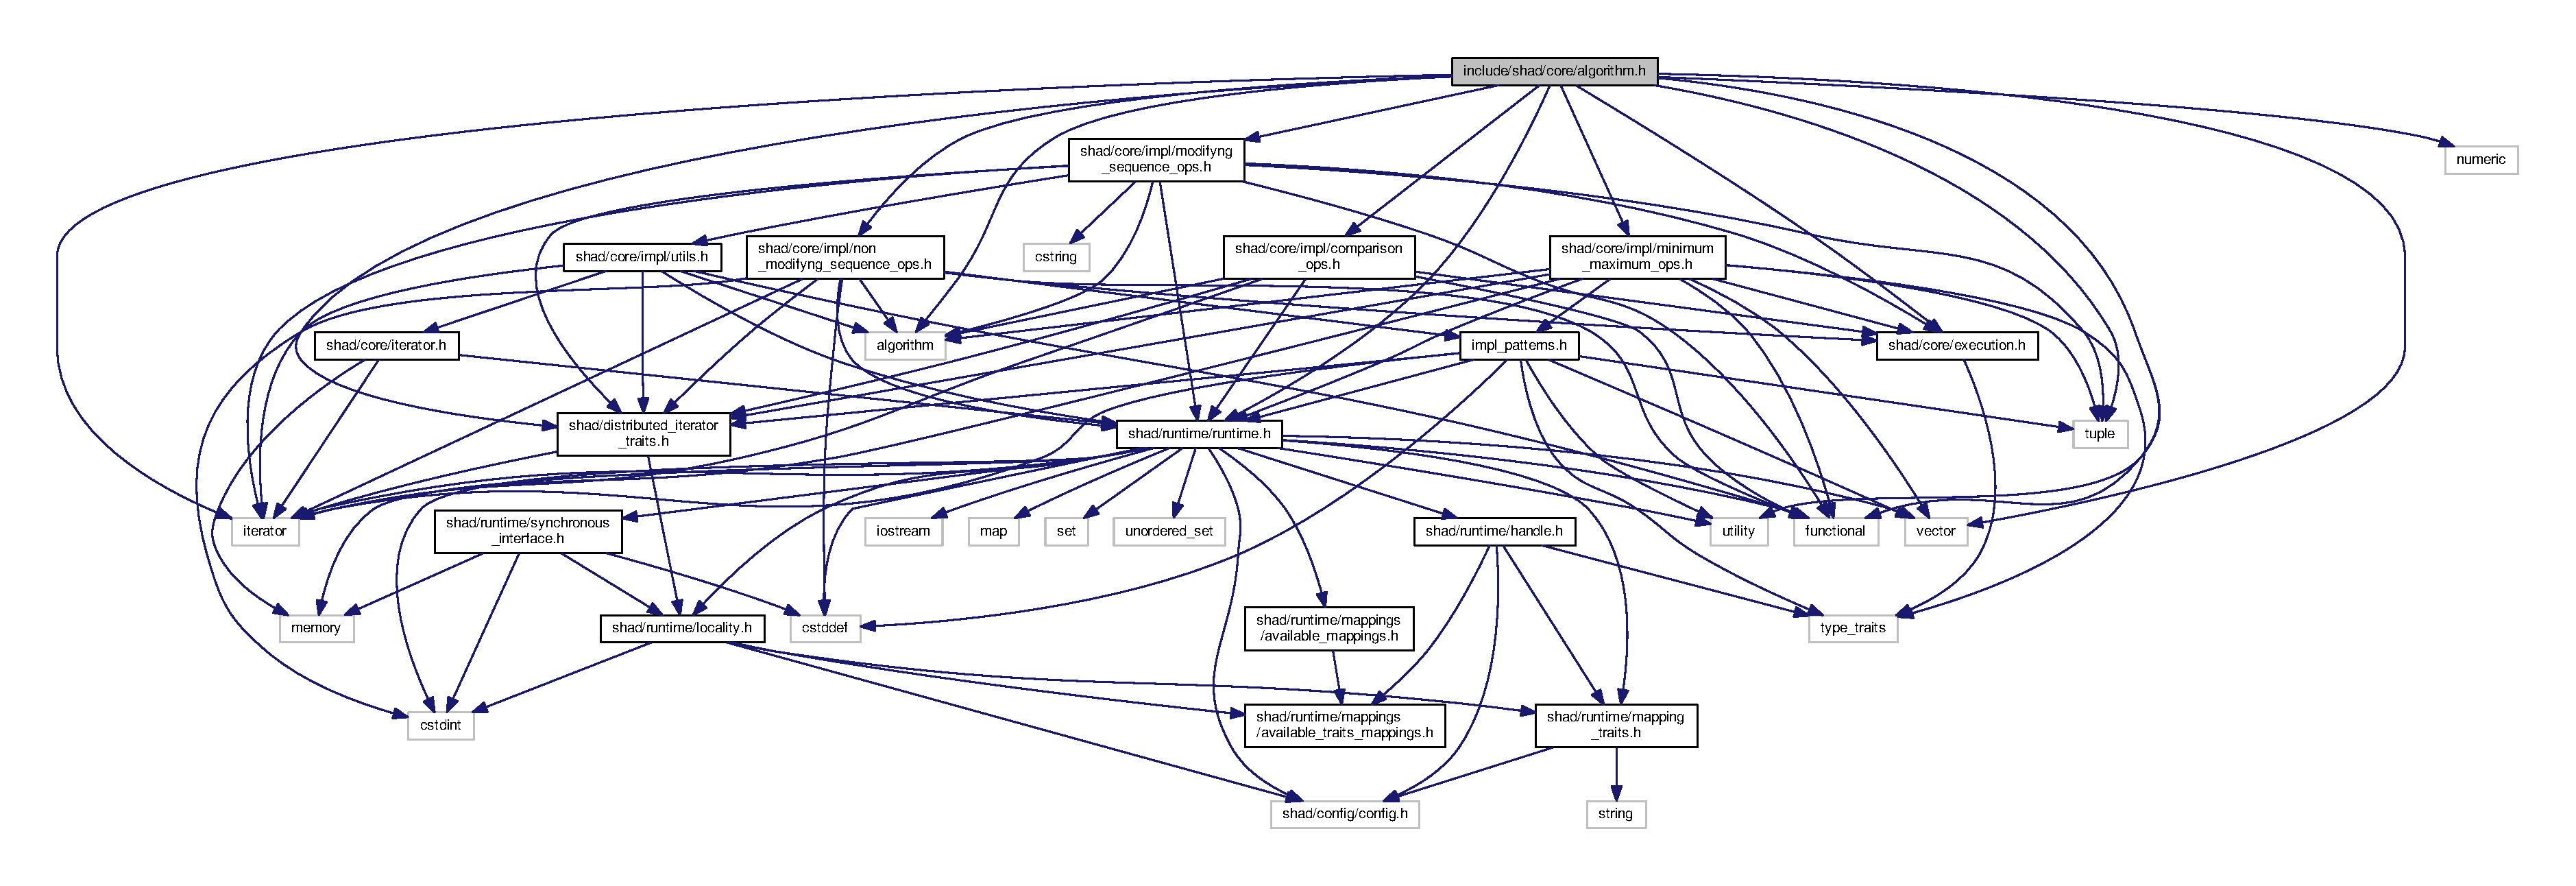
\includegraphics[width=350pt]{algorithm_8h__incl}
\end{center}
\end{figure}
\subsection*{Namespaces}
\begin{DoxyCompactItemize}
\item 
\hyperlink{namespaceshad}{shad}
\end{DoxyCompactItemize}
\subsection*{Functions}
\begin{DoxyCompactItemize}
\item 
{\footnotesize template$<$typename Execution\-Policy , typename Forward\-Itr , typename Unary\-Predicate $>$ }\\bool \hyperlink{namespaceshad_ab0314482e6cdabff5bcb7f2833b0f937}{shad\-::all\-\_\-of} (Execution\-Policy \&\&policy, Forward\-Itr first, Forward\-Itr last, Unary\-Predicate p)
\item 
{\footnotesize template$<$typename Execution\-Policy , typename Forward\-Itr , typename Unary\-Predicate $>$ }\\bool \hyperlink{namespaceshad_a8d17ad3a3f5f25ecfee20a7ae6ebf924}{shad\-::any\-\_\-of} (Execution\-Policy \&\&policy, Forward\-Itr first, Forward\-Itr last, Unary\-Predicate p)
\item 
{\footnotesize template$<$typename Execution\-Policy , typename Forward\-Itr , typename Unary\-Predicate $>$ }\\bool \hyperlink{namespaceshad_a00b17ed7d3482e7fc389d344c68b42e8}{shad\-::none\-\_\-of} (Execution\-Policy \&\&policy, Forward\-Itr first, Forward\-Itr last, Unary\-Predicate p)
\item 
{\footnotesize template$<$typename Execution\-Policy , typename Forward\-Itr , typename T $>$ }\\Forward\-Itr \hyperlink{namespaceshad_a63ec34eb3f98177db268051179d6057a}{shad\-::find} (Execution\-Policy \&\&policy, Forward\-Itr first, Forward\-Itr last, const T \&value)
\item 
{\footnotesize template$<$typename Execution\-Policy , typename Forward\-Itr , typename Unary\-Predicate $>$ }\\Forward\-Itr \hyperlink{namespaceshad_ae5272738a131b86c7d9349bfff977aa4}{shad\-::find\-\_\-if} (Execution\-Policy \&\&policy, Forward\-Itr first, Forward\-Itr last, Unary\-Predicate p)
\item 
{\footnotesize template$<$typename Execution\-Policy , typename Forward\-Itr , typename Unary\-Predicate $>$ }\\Forward\-Itr \hyperlink{namespaceshad_a42458d0084e37bb16f4745ee085aa2f5}{shad\-::find\-\_\-if\-\_\-not} (Execution\-Policy \&\&policy, Forward\-Itr first, Forward\-Itr last, Unary\-Predicate p)
\item 
{\footnotesize template$<$typename Execution\-Policy , typename Forward\-Itr , typename Unary\-Predicate $>$ }\\void \hyperlink{namespaceshad_a7daf2afb8d216454ff4143be21237d0c}{shad\-::for\-\_\-each} (Execution\-Policy \&\&policy, Forward\-Itr first, Forward\-Itr last, Unary\-Predicate p)
\item 
{\footnotesize template$<$typename Execution\-Policy , typename Input\-Itr , typename T $>$ }\\\hyperlink{structshad_1_1distributed__iterator__traits}{shad\-::distributed\-\_\-iterator\-\_\-traits}\\*
$<$ Input\-Itr $>$\-::difference\-\_\-type \hyperlink{namespaceshad_a2abc6976d67b071eccbb8d17e9a602fe}{shad\-::count} (Execution\-Policy \&\&policy, Input\-Itr first, Input\-Itr last, const T \&value)
\item 
{\footnotesize template$<$typename Execution\-Policy , typename Input\-Itr , typename Unary\-Predicate $>$ }\\\hyperlink{structshad_1_1distributed__iterator__traits}{shad\-::distributed\-\_\-iterator\-\_\-traits}\\*
$<$ Input\-Itr $>$\-::difference\-\_\-type \hyperlink{namespaceshad_a08f4233aef9435fb627ebb82d186715e}{shad\-::count\-\_\-if} (Execution\-Policy \&\&policy, Input\-Itr first, Input\-Itr last, Unary\-Predicate p)
\item 
{\footnotesize template$<$class Forward\-It $>$ }\\Forward\-It \hyperlink{namespaceshad_a81976ee44edd512260a625c628f6094b}{shad\-::max\-\_\-element} (Forward\-It first, Forward\-It last)
\item 
{\footnotesize template$<$class Execution\-Policy , class Forward\-It $>$ }\\std\-::enable\-\_\-if\-\_\-t\\*
$<$ \hyperlink{structshad_1_1is__execution__policy}{shad\-::is\-\_\-execution\-\_\-policy}\\*
$<$ Execution\-Policy $>$\-::value, \\*
Forward\-It $>$ \hyperlink{namespaceshad_a3f4b06918fc7b1425c9bc8aa942d894d}{shad\-::max\-\_\-element} (Execution\-Policy \&\&policy, Forward\-It first, Forward\-It last)
\item 
{\footnotesize template$<$class Forward\-It , class Compare $>$ }\\std\-::enable\-\_\-if\-\_\-t\\*
$<$!\hyperlink{structshad_1_1is__execution__policy}{shad\-::is\-\_\-execution\-\_\-policy}\\*
$<$ Forward\-It $>$\-::value, \\*
Forward\-It $>$ \hyperlink{namespaceshad_aceab28870f92123bc4489897c5e7d640}{shad\-::max\-\_\-element} (Forward\-It first, Forward\-It last, Compare comp)
\item 
{\footnotesize template$<$class Execution\-Policy , class Forward\-It , class Compare $>$ }\\Forward\-It \hyperlink{namespaceshad_a507fdc64c5881f464e3c6dd7e470bfa1}{shad\-::max\-\_\-element} (Execution\-Policy \&\&policy, Forward\-It first, Forward\-It last, Compare comp)
\item 
{\footnotesize template$<$class Forward\-It $>$ }\\Forward\-It \hyperlink{namespaceshad_a8fa362bdd1e3f20d68a86f80cd5d47e5}{shad\-::min\-\_\-element} (Forward\-It first, Forward\-It last)
\item 
{\footnotesize template$<$class Execution\-Policy , class Forward\-It $>$ }\\std\-::enable\-\_\-if\-\_\-t\\*
$<$ \hyperlink{structshad_1_1is__execution__policy}{shad\-::is\-\_\-execution\-\_\-policy}\\*
$<$ Execution\-Policy $>$\-::value, \\*
Forward\-It $>$ \hyperlink{namespaceshad_ab2b1735a5a797bce70247ebf95081238}{shad\-::min\-\_\-element} (Execution\-Policy \&\&policy, Forward\-It first, Forward\-It last)
\item 
{\footnotesize template$<$class Forward\-It , class Compare $>$ }\\std\-::enable\-\_\-if\-\_\-t\\*
$<$!\hyperlink{structshad_1_1is__execution__policy}{shad\-::is\-\_\-execution\-\_\-policy}\\*
$<$ Forward\-It $>$\-::value, \\*
Forward\-It $>$ \hyperlink{namespaceshad_aaea0353fe93d75d2a5dbe4409921a25e}{shad\-::min\-\_\-element} (Forward\-It first, Forward\-It last, Compare comp)
\item 
{\footnotesize template$<$class Execution\-Policy , class Forward\-It , class Compare $>$ }\\Forward\-It \hyperlink{namespaceshad_ade79004d9d2b57d94717640536689f30}{shad\-::min\-\_\-element} (Execution\-Policy \&\&policy, Forward\-It first, Forward\-It last, Compare comp)
\item 
{\footnotesize template$<$class Forward\-It $>$ }\\std\-::pair$<$ Forward\-It, Forward\-It $>$ \hyperlink{namespaceshad_a04498eaaa7278dc429fcdf93f5915bfd}{shad\-::minmax\-\_\-element} (Forward\-It first, Forward\-It last)
\item 
{\footnotesize template$<$class Execution\-Policy , class Forward\-It $>$ }\\std\-::enable\-\_\-if\-\_\-t\\*
$<$ \hyperlink{structshad_1_1is__execution__policy}{shad\-::is\-\_\-execution\-\_\-policy}\\*
$<$ Execution\-Policy $>$\-::value, \\*
std\-::pair$<$ Forward\-It, \\*
Forward\-It $>$ $>$ \hyperlink{namespaceshad_af24b9e8c34031c3eb513512540d75220}{shad\-::minmax\-\_\-element} (Execution\-Policy \&\&policy, Forward\-It first, Forward\-It last)
\item 
{\footnotesize template$<$class Forward\-It , class Compare $>$ }\\std\-::enable\-\_\-if\-\_\-t\\*
$<$!\hyperlink{structshad_1_1is__execution__policy}{shad\-::is\-\_\-execution\-\_\-policy}\\*
$<$ Forward\-It $>$\-::value, \\*
std\-::pair$<$ Forward\-It, \\*
Forward\-It $>$ $>$ \hyperlink{namespaceshad_a16fcfebd88d79295c4f5ff4762e17329}{shad\-::minmax\-\_\-element} (Forward\-It first, Forward\-It last, Compare comp)
\item 
{\footnotesize template$<$class Execution\-Policy , class Forward\-It , class Compare $>$ }\\std\-::pair$<$ Forward\-It, Forward\-It $>$ \hyperlink{namespaceshad_a19b6f97e22a10d008622ad4e49de5f6b}{shad\-::minmax\-\_\-element} (Execution\-Policy \&\&policy, Forward\-It first, Forward\-It last, Compare comp)
\item 
{\footnotesize template$<$class Execution\-Policy , class Forward\-It , class T $>$ }\\void \hyperlink{namespaceshad_ab21c74ec57b46160ad590b2e989c4ea6}{shad\-::fill} (Execution\-Policy \&\&policy, Forward\-It first, Forward\-It last, const T \&value)
\item 
{\footnotesize template$<$class Execution\-Policy , class Forward\-It1 , class Forward\-It2 , class Unary\-Operation $>$ }\\Forward\-It2 \hyperlink{namespaceshad_a7a39d855612f2a2957f27b7571e9dc54}{shad\-::transform} (Execution\-Policy \&\&policy, Forward\-It1 first1, Forward\-It1 last1, Forward\-It2 d\-\_\-first, Unary\-Operation unary\-\_\-op)
\item 
{\footnotesize template$<$class Execution\-Policy , class Forward\-It , class Generator $>$ }\\void \hyperlink{namespaceshad_a9bd5736fe5e18ec23a7d7e5913a11df8}{shad\-::generate} (Execution\-Policy \&\&policy, Forward\-It first, Forward\-It last, Generator g)
\item 
{\footnotesize template$<$class Execution\-Policy , class Forward\-It , class T $>$ }\\void \hyperlink{namespaceshad_a0c0ef45cc72fdfcc83ec82af01154289}{shad\-::replace} (Execution\-Policy \&\&policy, Forward\-It first, Forward\-It last, const T \&old\-\_\-value, const T \&new\-\_\-value)
\item 
{\footnotesize template$<$class Execution\-Policy , class Forward\-It , class Unary\-Predicate , class T $>$ }\\void \hyperlink{namespaceshad_aef6165d38034e9fd6e2fa8bb433a6f61}{shad\-::replace\-\_\-if} (Execution\-Policy \&\&policy, Forward\-It first, Forward\-It last, Unary\-Predicate p, const T \&new\-\_\-value)
\item 
{\footnotesize template$<$class Input\-It1 , class Input\-It2 $>$ }\\bool \hyperlink{namespaceshad_a8141e857a877c6eb44095a7578281ecd}{shad\-::equal} (Input\-It1 first1, Input\-It1 last1, Input\-It2 first2)
\item 
{\footnotesize template$<$class Execution\-Policy , class Forward\-It1 , class Forward\-It2 $>$ }\\std\-::enable\-\_\-if\-\_\-t\\*
$<$ \hyperlink{structshad_1_1is__execution__policy}{shad\-::is\-\_\-execution\-\_\-policy}\\*
$<$ Execution\-Policy $>$\-::value, \\*
bool $>$ \hyperlink{namespaceshad_ad909faa4c50e8fe776668cd39e776602}{shad\-::equal} (Execution\-Policy \&\&policy, Forward\-It1 first1, Forward\-It1 last1, Forward\-It2 first2)
\item 
{\footnotesize template$<$class Input\-It1 , class Input\-It2 , class Binary\-Predicate $>$ }\\std\-::enable\-\_\-if\-\_\-t$<$!std\-::is\-\_\-same\\*
$<$ Input\-It2, Binary\-Predicate $>$\\*
\-::value, bool $>$ \hyperlink{namespaceshad_a9be869b9241eafbec6af016a45fa8f45}{shad\-::equal} (Input\-It1 first1, Input\-It1 last1, Input\-It2 first2, Binary\-Predicate p)
\item 
{\footnotesize template$<$class Execution\-Policy , class Forward\-It1 , class Forward\-It2 , class Binary\-Predicate $>$ }\\std\-::enable\-\_\-if\-\_\-t\\*
$<$(\hyperlink{structshad_1_1is__execution__policy}{shad\-::is\-\_\-execution\-\_\-policy}\\*
$<$ Execution\-Policy $>$\-::value \\*
\&\&!std\-::is\-\_\-same$<$ Forward\-It2, \\*
Binary\-Predicate $>$\-::value), \\*
bool $>$ \hyperlink{namespaceshad_a1d99da6ce33f2013b3ff47b9a05a0916}{shad\-::equal} (Execution\-Policy \&\&policy, Forward\-It1 first1, Forward\-It1 last1, Forward\-It2 first2, Binary\-Predicate p)
\item 
{\footnotesize template$<$class Input\-It1 , class Input\-It2 $>$ }\\bool \hyperlink{namespaceshad_aa5dcd90777a8948f8cb240d51bd1346b}{shad\-::equal} (Input\-It1 first1, Input\-It1 last1, Input\-It2 first2, Input\-It2 last2)
\item 
{\footnotesize template$<$class Execution\-Policy , class Forward\-It1 , class Forward\-It2 $>$ }\\std\-::enable\-\_\-if\-\_\-t\\*
$<$ \hyperlink{structshad_1_1is__execution__policy}{shad\-::is\-\_\-execution\-\_\-policy}\\*
$<$ Execution\-Policy $>$\-::value, \\*
bool $>$ \hyperlink{namespaceshad_ae452511628cb333e23458bb2af8cfa83}{shad\-::equal} (Execution\-Policy \&\&policy, Forward\-It1 first1, Forward\-It1 last1, Forward\-It2 first2, Forward\-It2 last2)
\item 
{\footnotesize template$<$class Input\-It1 , class Input\-It2 , class Binary\-Predicate $>$ }\\std\-::enable\-\_\-if\-\_\-t$<$!std\-::is\-\_\-same\\*
$<$ Input\-It2, Binary\-Predicate $>$\\*
\-::value, bool $>$ \hyperlink{namespaceshad_a729216b8f76b721c9e1ae8fdcb63ee03}{shad\-::equal} (Input\-It1 first1, Input\-It1 last1, Input\-It2 first2, Input\-It2 last2, Binary\-Predicate p)
\item 
{\footnotesize template$<$class Execution\-Policy , class Forward\-It1 , class Forward\-It2 , class Binary\-Predicate $>$ }\\bool \hyperlink{namespaceshad_a8566c24e54c82d15757af3f776c54c40}{shad\-::equal} (Execution\-Policy \&\&policy, Forward\-It1 first1, Forward\-It1 last1, Forward\-It2 first2, Forward\-It2 last2, Binary\-Predicate p)
\item 
{\footnotesize template$<$class Input\-It1 , class Input\-It2 $>$ }\\bool \hyperlink{namespaceshad_a65aac88682894c75b4b1caee38cc9c8f}{shad\-::lexicographical\-\_\-compare} (Input\-It1 first1, Input\-It1 last1, Input\-It2 first2, Input\-It2 last2)
\item 
{\footnotesize template$<$class Execution\-Policy , class Forward\-It1 , class Forward\-It2 $>$ }\\std\-::enable\-\_\-if\-\_\-t\\*
$<$ \hyperlink{structshad_1_1is__execution__policy}{shad\-::is\-\_\-execution\-\_\-policy}\\*
$<$ Execution\-Policy $>$\-::value, \\*
bool $>$ \hyperlink{namespaceshad_a060c390865e5dbec41c7e2526fae8803}{shad\-::lexicographical\-\_\-compare} (Execution\-Policy \&\&policy, Forward\-It1 first1, Forward\-It1 last1, Forward\-It2 first2, Forward\-It2 last2)
\item 
{\footnotesize template$<$class Input\-It1 , class Input\-It2 , class Compare $>$ }\\std\-::enable\-\_\-if\-\_\-t\\*
$<$!\hyperlink{structshad_1_1is__execution__policy}{shad\-::is\-\_\-execution\-\_\-policy}\\*
$<$ Input\-It1 $>$\-::value, bool $>$ \hyperlink{namespaceshad_a05a181e15eb05bb17cf7bedcacc98585}{shad\-::lexicographical\-\_\-compare} (Input\-It1 first1, Input\-It1 last1, Input\-It2 first2, Input\-It2 last2, Compare comp)
\item 
{\footnotesize template$<$class Execution\-Policy , class Forward\-It1 , class Forward\-It2 , class Compare $>$ }\\bool \hyperlink{namespaceshad_a10090ea72775e10b015408d8c9050ac3}{shad\-::lexicographical\-\_\-compare} (Execution\-Policy \&\&policy, Forward\-It1 first1, Forward\-It1 last1, Forward\-It2 first2, Forward\-It2 last2, Compare comp)
\end{DoxyCompactItemize}

\hypertarget{core_2array_8h}{\section{include/shad/core/array.h File Reference}
\label{core_2array_8h}\index{include/shad/core/array.\-h@{include/shad/core/array.\-h}}
}
{\ttfamily \#include $<$cstdlib$>$}\\*
{\ttfamily \#include \char`\"{}shad/data\-\_\-structures/abstract\-\_\-data\-\_\-structure.\-h\char`\"{}}\\*
{\ttfamily \#include \char`\"{}shad/distributed\-\_\-iterator\-\_\-traits.\-h\char`\"{}}\\*
{\ttfamily \#include \char`\"{}shad/runtime/runtime.\-h\char`\"{}}\\*
Include dependency graph for array.\-h\-:
\nopagebreak
\begin{figure}[H]
\begin{center}
\leavevmode
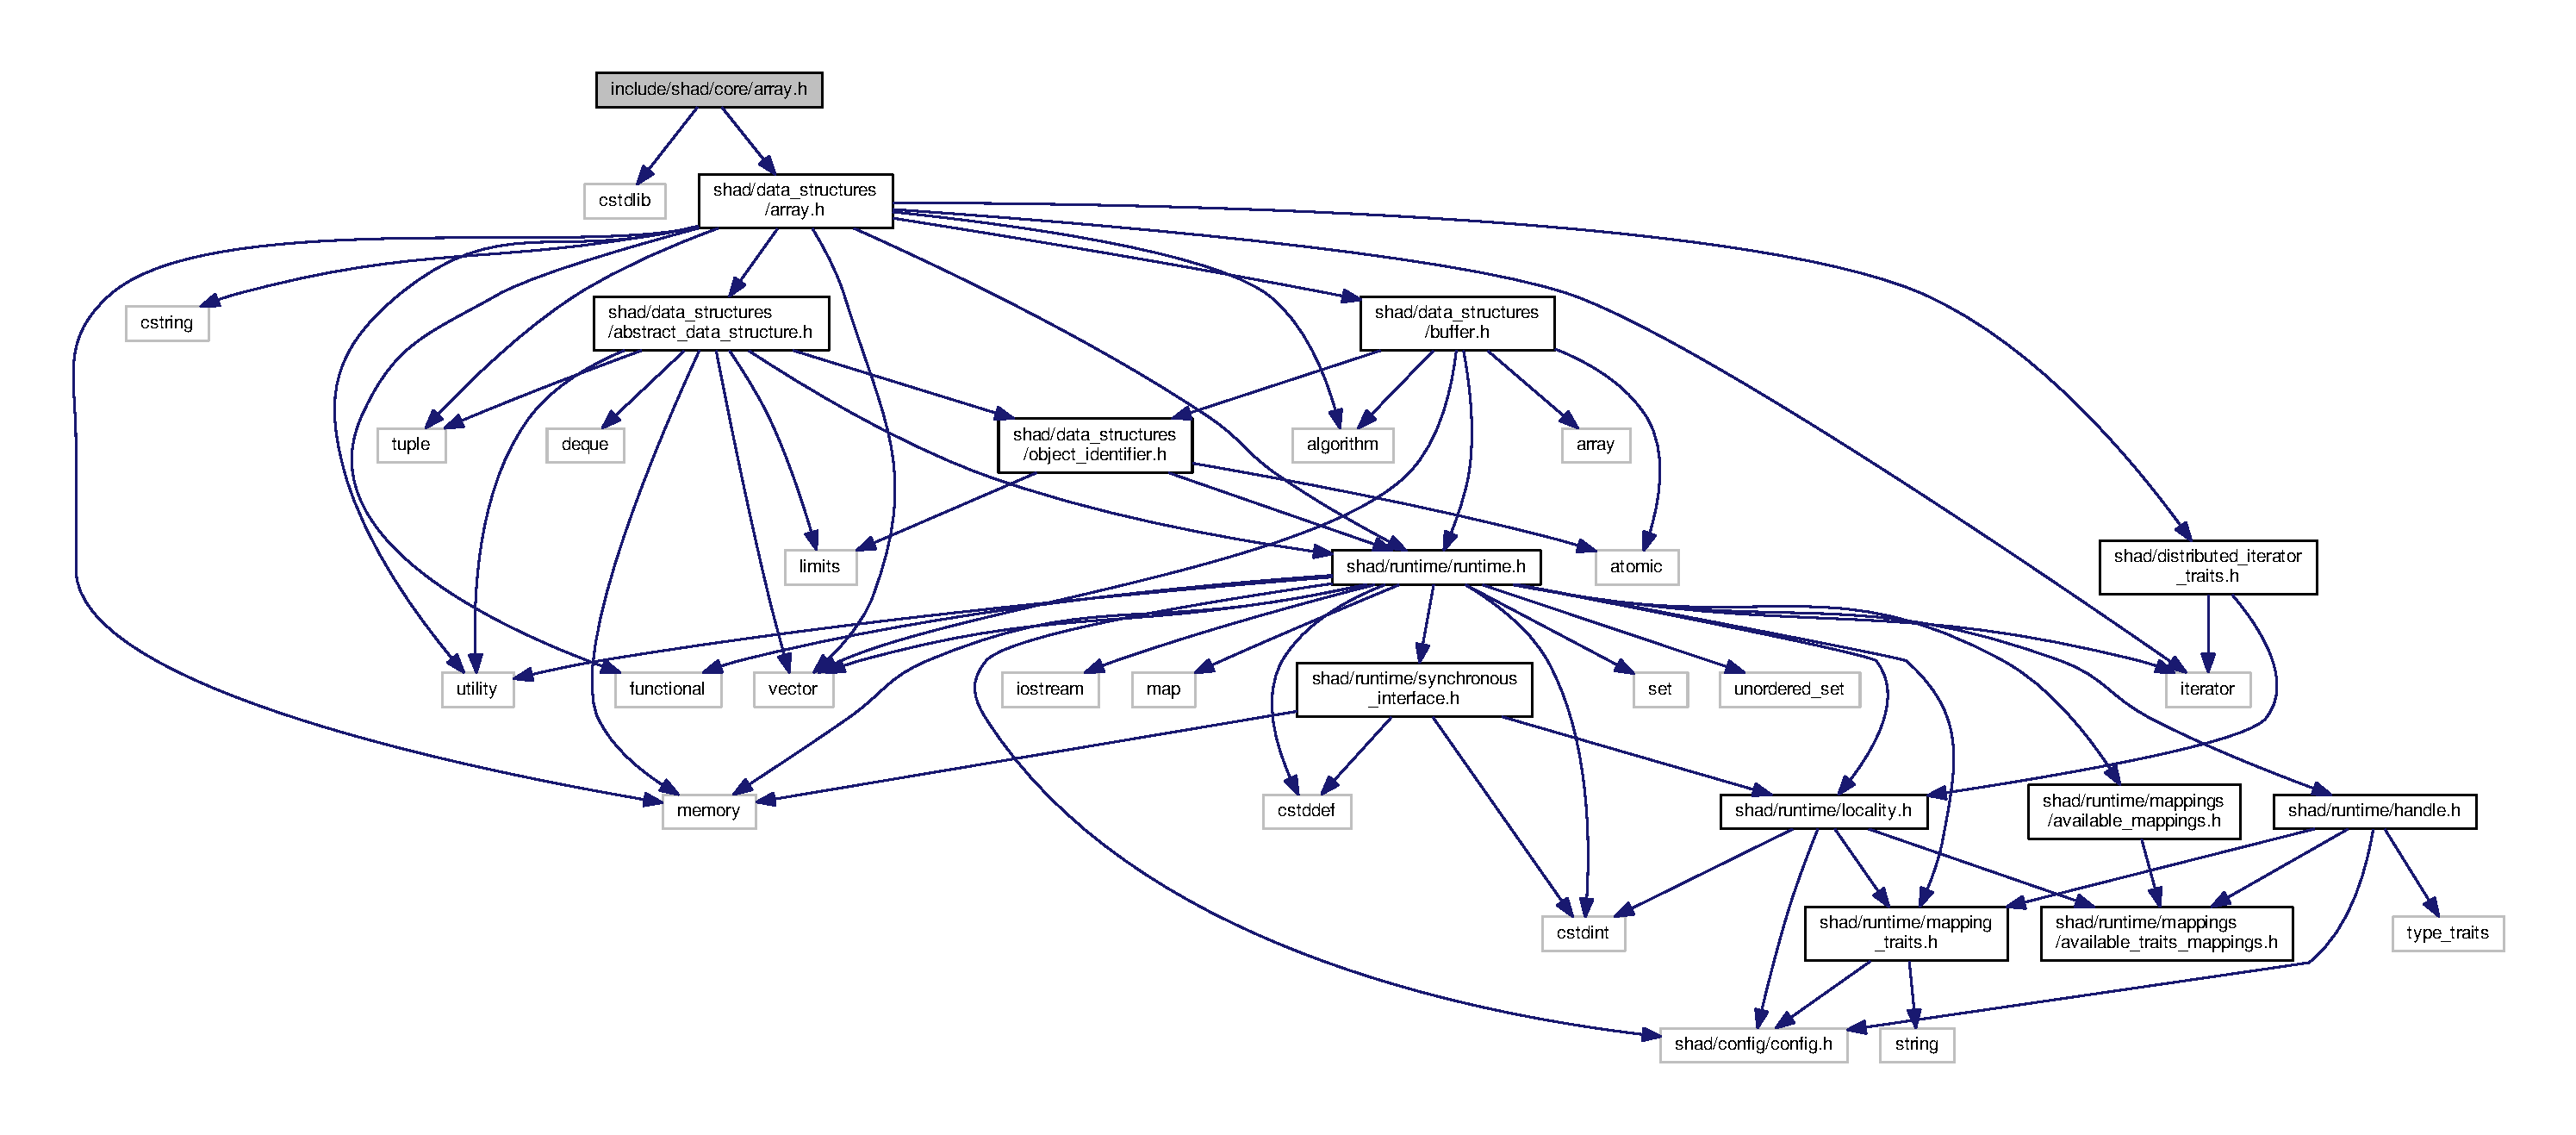
\includegraphics[width=350pt]{core_2array_8h__incl}
\end{center}
\end{figure}
\subsection*{Classes}
\begin{DoxyCompactItemize}
\item 
class \hyperlink{classshad_1_1array}{shad\-::array$<$ T, N $>$}
\begin{DoxyCompactList}\small\item\em Fixed size distributed array. \end{DoxyCompactList}\end{DoxyCompactItemize}
\subsection*{Namespaces}
\begin{DoxyCompactItemize}
\item 
\hyperlink{namespaceshad}{shad}
\end{DoxyCompactItemize}

\hypertarget{data__structures_2array_8h}{\section{include/shad/data\-\_\-structures/array.h File Reference}
\label{data__structures_2array_8h}\index{include/shad/data\-\_\-structures/array.\-h@{include/shad/data\-\_\-structures/array.\-h}}
}
{\ttfamily \#include $<$algorithm$>$}\\*
{\ttfamily \#include $<$cstring$>$}\\*
{\ttfamily \#include $<$functional$>$}\\*
{\ttfamily \#include $<$iterator$>$}\\*
{\ttfamily \#include $<$memory$>$}\\*
{\ttfamily \#include $<$tuple$>$}\\*
{\ttfamily \#include $<$utility$>$}\\*
{\ttfamily \#include $<$vector$>$}\\*
{\ttfamily \#include \char`\"{}shad/data\-\_\-structures/abstract\-\_\-data\-\_\-structure.\-h\char`\"{}}\\*
{\ttfamily \#include \char`\"{}shad/data\-\_\-structures/buffer.\-h\char`\"{}}\\*
{\ttfamily \#include \char`\"{}shad/runtime/runtime.\-h\char`\"{}}\\*
Include dependency graph for array.\-h\-:
\nopagebreak
\begin{figure}[H]
\begin{center}
\leavevmode
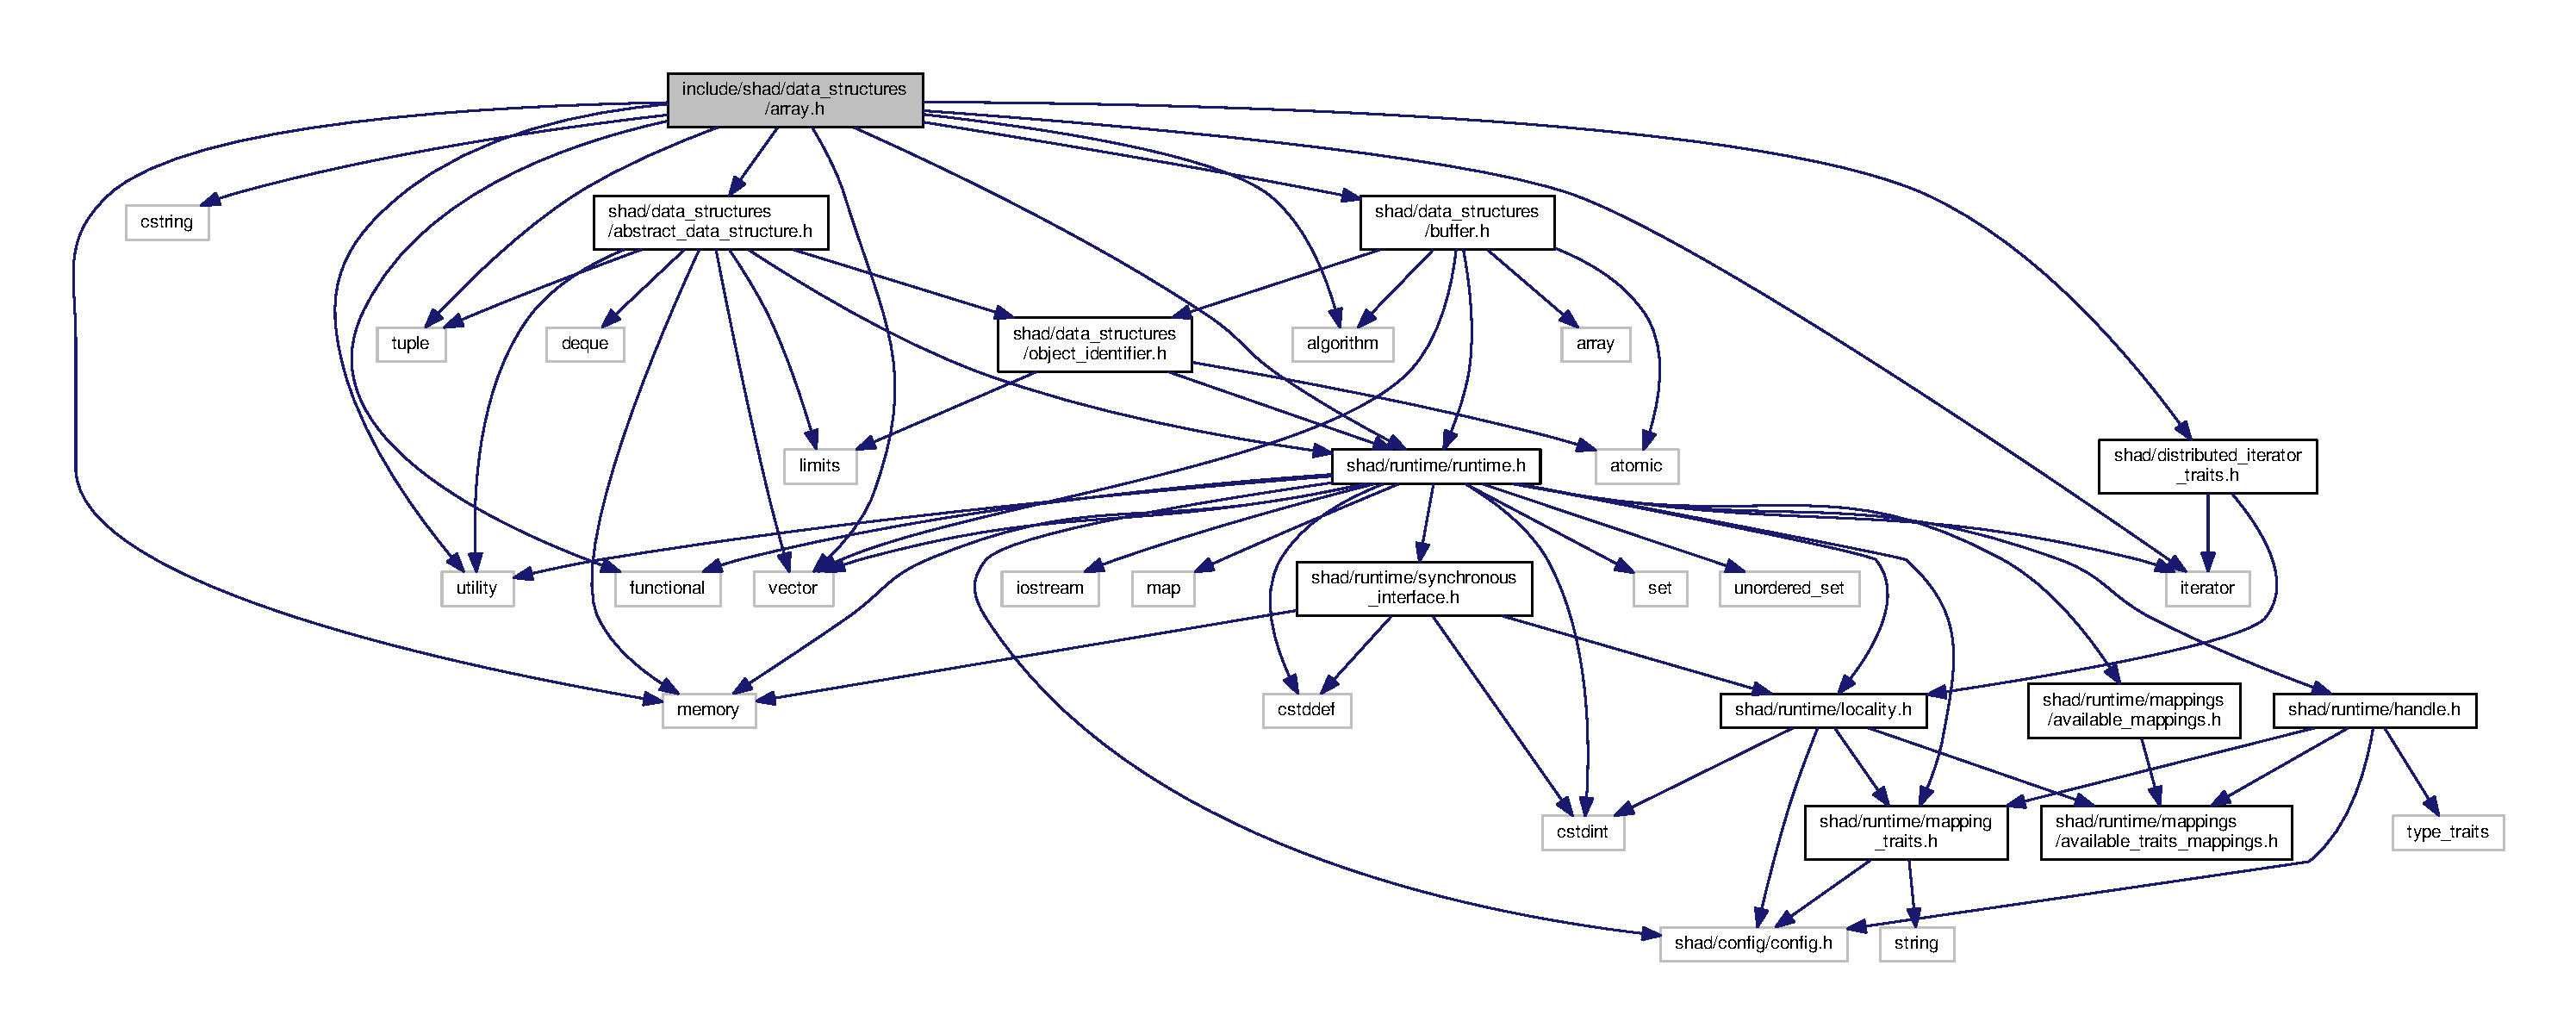
\includegraphics[width=350pt]{data__structures_2array_8h__incl}
\end{center}
\end{figure}
This graph shows which files directly or indirectly include this file\-:
\nopagebreak
\begin{figure}[H]
\begin{center}
\leavevmode
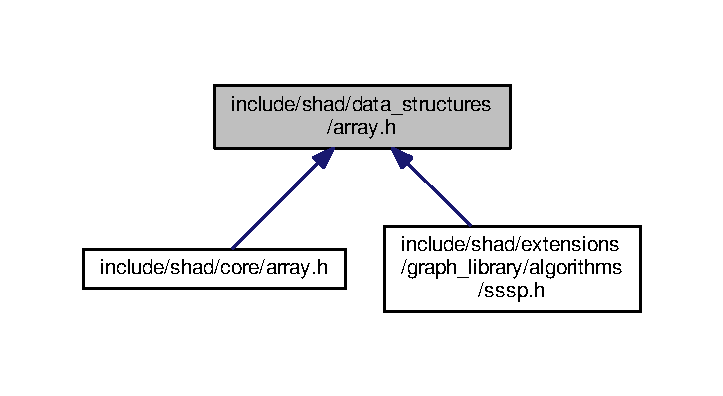
\includegraphics[width=222pt]{data__structures_2array_8h__dep__incl}
\end{center}
\end{figure}
\subsection*{Classes}
\begin{DoxyCompactItemize}
\item 
class \hyperlink{classshad_1_1Array}{shad\-::\-Array$<$ T $>$}
\begin{DoxyCompactList}\small\item\em The \hyperlink{classshad_1_1Array}{Array} data structure. \end{DoxyCompactList}\end{DoxyCompactItemize}
\subsection*{Namespaces}
\begin{DoxyCompactItemize}
\item 
\hyperlink{namespaceshad}{shad}
\end{DoxyCompactItemize}

\hypertarget{execution_8h}{\section{include/shad/core/execution.h File Reference}
\label{execution_8h}\index{include/shad/core/execution.\-h@{include/shad/core/execution.\-h}}
}
This graph shows which files directly or indirectly include this file\-:
\nopagebreak
\begin{figure}[H]
\begin{center}
\leavevmode
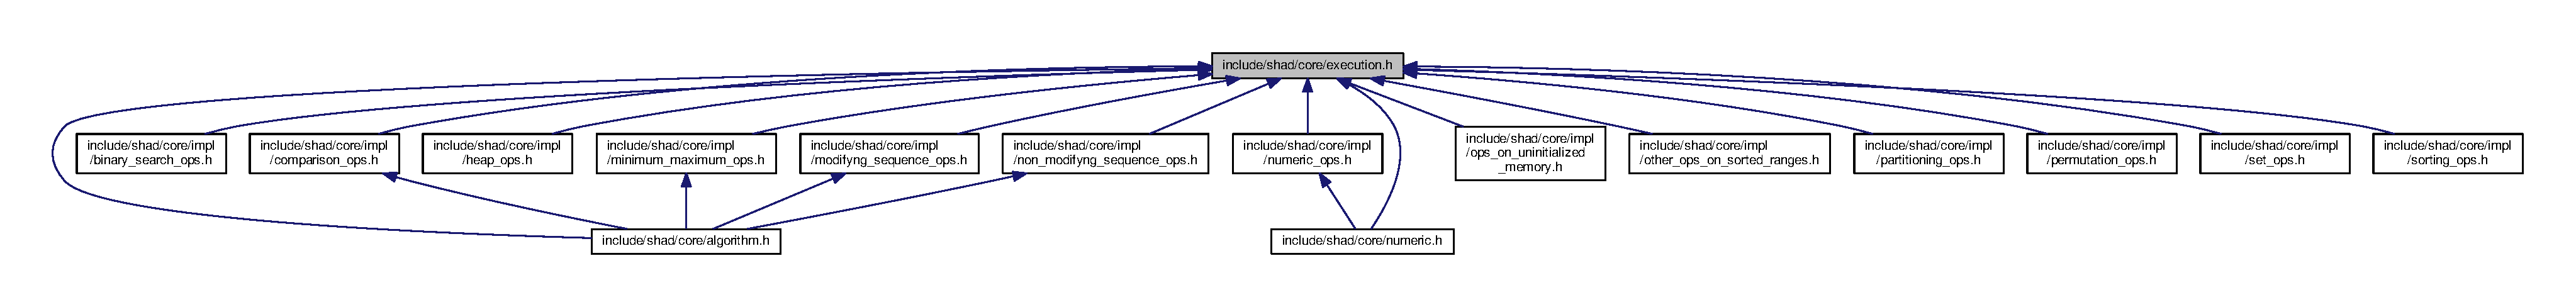
\includegraphics[width=226pt]{execution_8h__dep__incl}
\end{center}
\end{figure}
\subsection*{Classes}
\begin{DoxyCompactItemize}
\item 
struct \hyperlink{structshad_1_1distributed__sequential__tag}{shad\-::distributed\-\_\-sequential\-\_\-tag}
\item 
struct \hyperlink{structshad_1_1distributed__parallel__tag}{shad\-::distributed\-\_\-parallel\-\_\-tag}
\end{DoxyCompactItemize}
\subsection*{Namespaces}
\begin{DoxyCompactItemize}
\item 
\hyperlink{namespaceshad}{shad}
\end{DoxyCompactItemize}

\hypertarget{binary__search__ops_8h}{\section{include/shad/core/impl/binary\-\_\-search\-\_\-ops.h File Reference}
\label{binary__search__ops_8h}\index{include/shad/core/impl/binary\-\_\-search\-\_\-ops.\-h@{include/shad/core/impl/binary\-\_\-search\-\_\-ops.\-h}}
}
{\ttfamily \#include $<$algorithm$>$}\\*
{\ttfamily \#include $<$functional$>$}\\*
{\ttfamily \#include $<$iterator$>$}\\*
{\ttfamily \#include \char`\"{}shad/core/execution.\-h\char`\"{}}\\*
{\ttfamily \#include \char`\"{}shad/distributed\-\_\-iterator\-\_\-traits.\-h\char`\"{}}\\*
{\ttfamily \#include \char`\"{}shad/runtime/runtime.\-h\char`\"{}}\\*
Include dependency graph for binary\-\_\-search\-\_\-ops.\-h\-:
\nopagebreak
\begin{figure}[H]
\begin{center}
\leavevmode
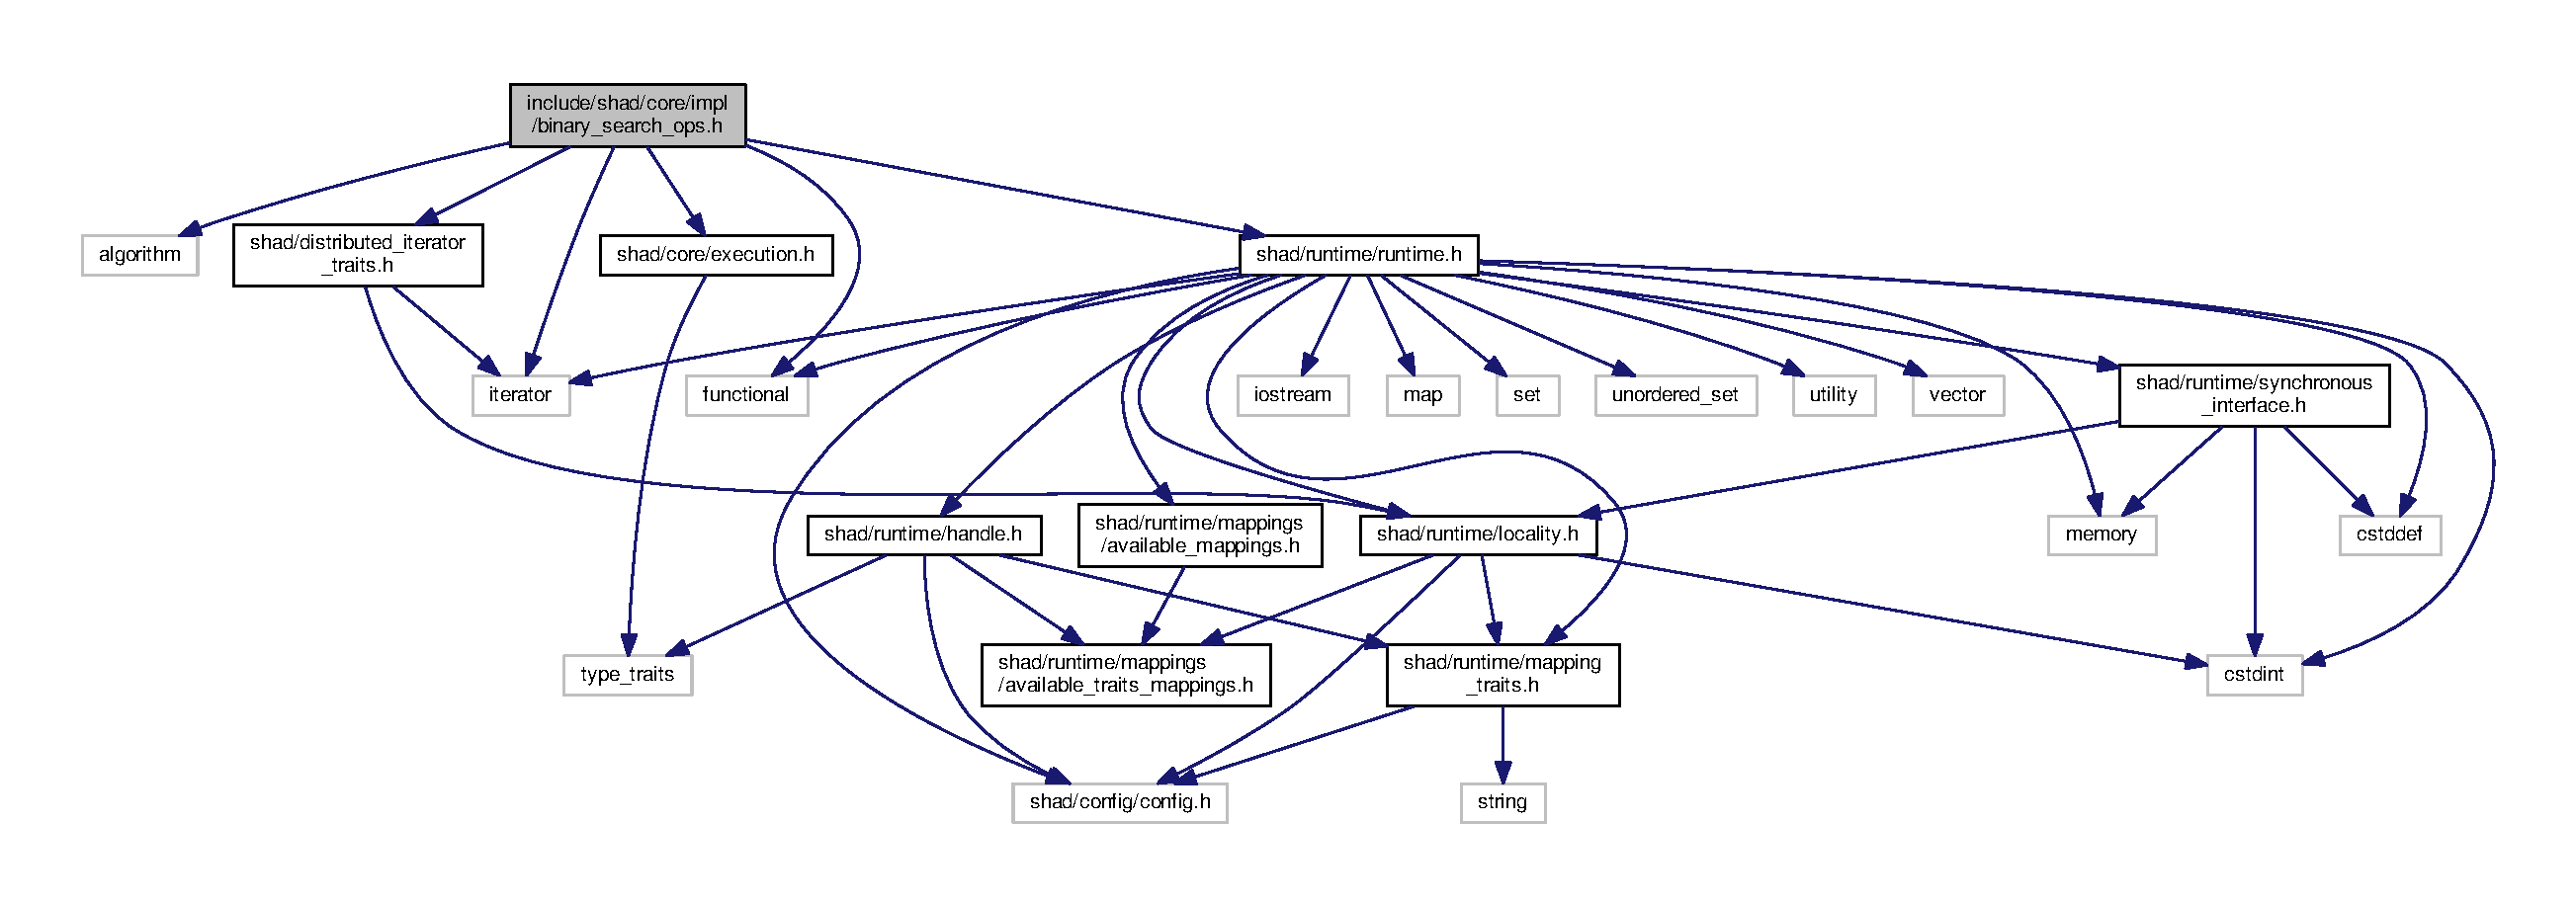
\includegraphics[width=350pt]{binary__search__ops_8h__incl}
\end{center}
\end{figure}
\subsection*{Namespaces}
\begin{DoxyCompactItemize}
\item 
\hyperlink{namespaceshad}{shad}
\end{DoxyCompactItemize}

\hypertarget{comparison__ops_8h}{\section{include/shad/core/impl/comparison\-\_\-ops.h File Reference}
\label{comparison__ops_8h}\index{include/shad/core/impl/comparison\-\_\-ops.\-h@{include/shad/core/impl/comparison\-\_\-ops.\-h}}
}
{\ttfamily \#include $<$algorithm$>$}\\*
{\ttfamily \#include $<$functional$>$}\\*
{\ttfamily \#include $<$iterator$>$}\\*
{\ttfamily \#include \char`\"{}shad/core/execution.\-h\char`\"{}}\\*
{\ttfamily \#include \char`\"{}shad/distributed\-\_\-iterator\-\_\-traits.\-h\char`\"{}}\\*
{\ttfamily \#include \char`\"{}shad/runtime/runtime.\-h\char`\"{}}\\*
Include dependency graph for comparison\-\_\-ops.\-h\-:
\nopagebreak
\begin{figure}[H]
\begin{center}
\leavevmode
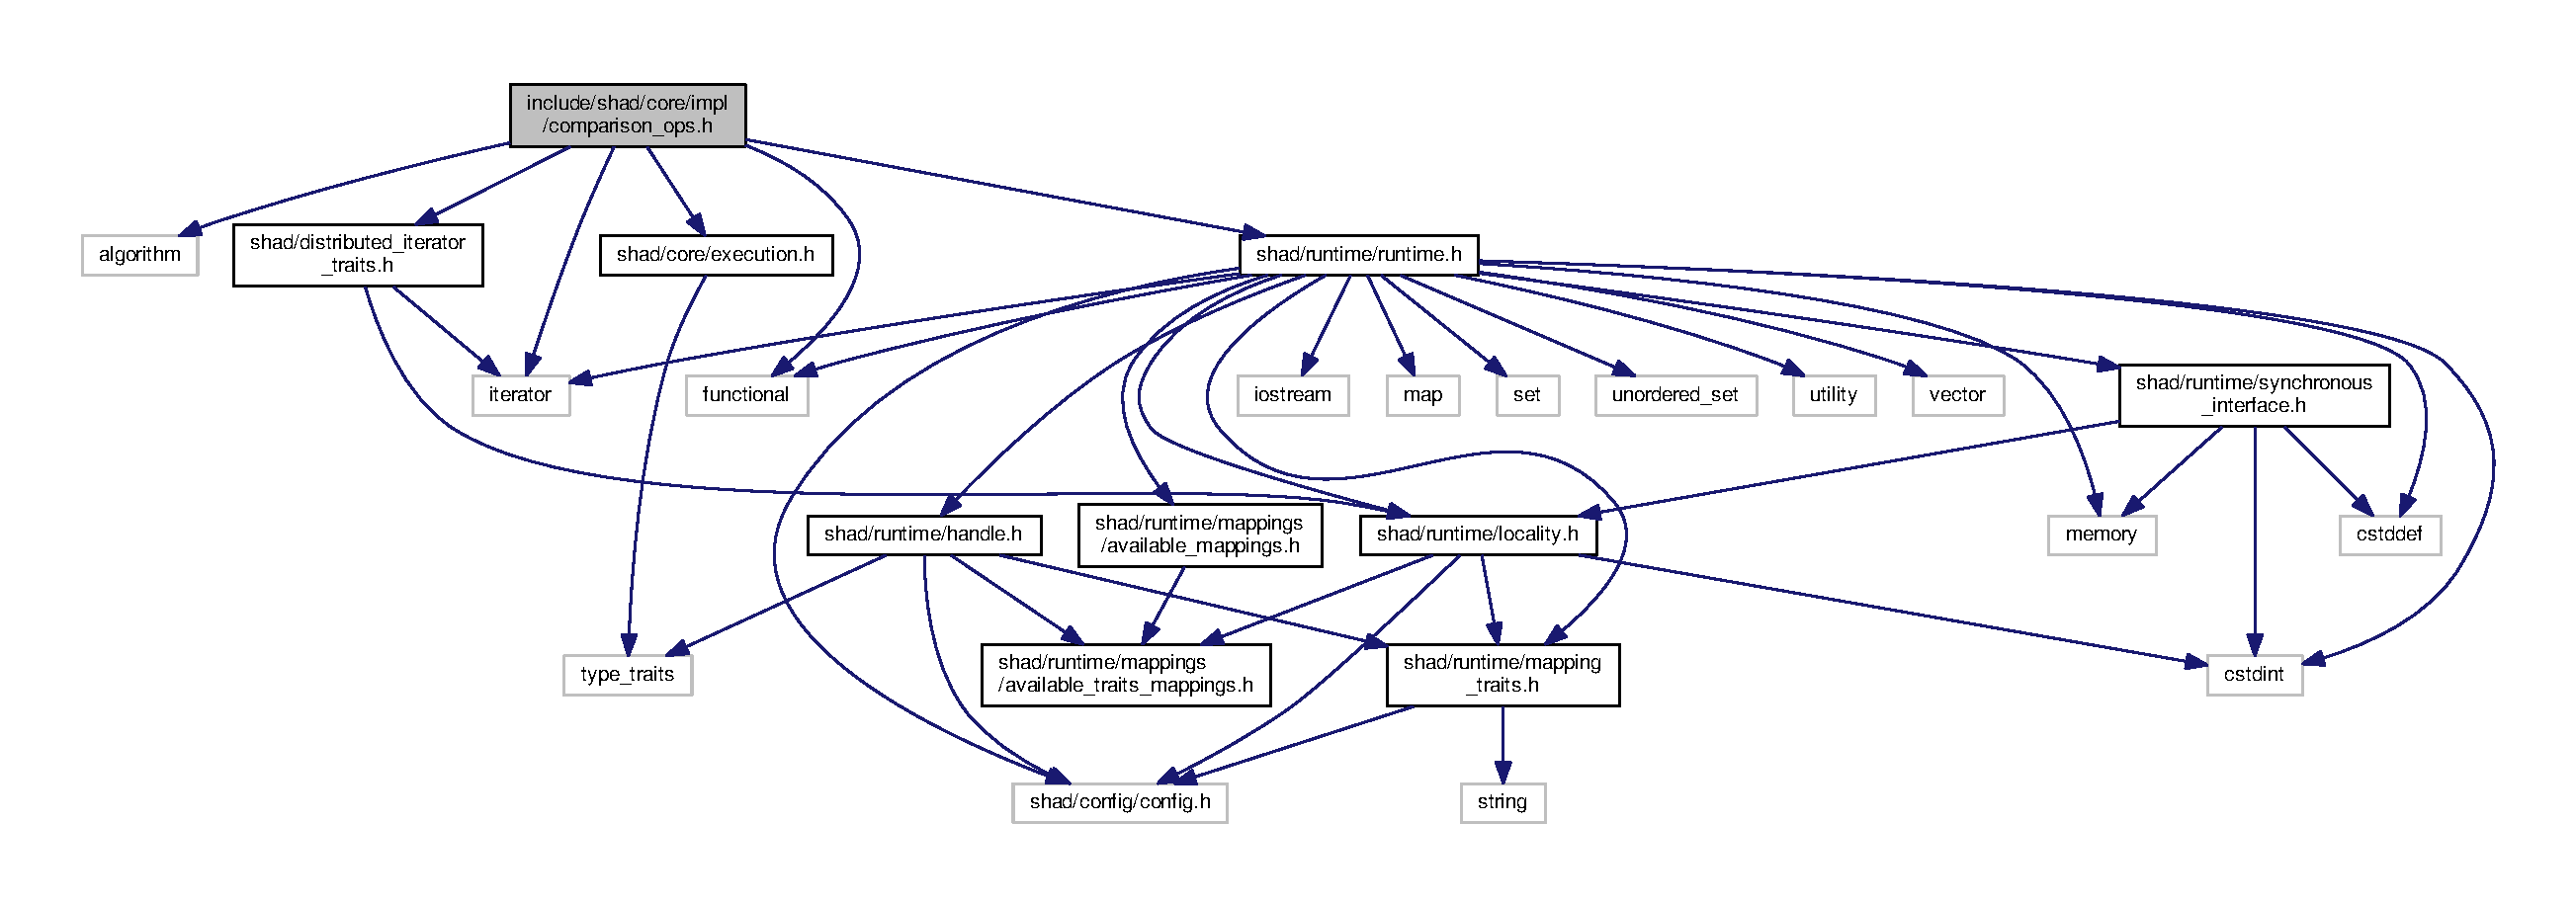
\includegraphics[width=350pt]{comparison__ops_8h__incl}
\end{center}
\end{figure}
This graph shows which files directly or indirectly include this file\-:
\nopagebreak
\begin{figure}[H]
\begin{center}
\leavevmode
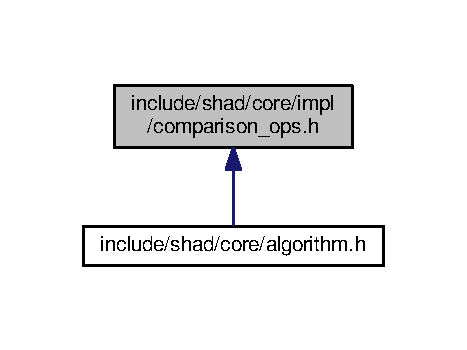
\includegraphics[width=224pt]{comparison__ops_8h__dep__incl}
\end{center}
\end{figure}
\subsection*{Namespaces}
\begin{DoxyCompactItemize}
\item 
\hyperlink{namespaceshad}{shad}
\end{DoxyCompactItemize}

\hypertarget{heap__ops_8h}{\section{include/shad/core/impl/heap\-\_\-ops.h File Reference}
\label{heap__ops_8h}\index{include/shad/core/impl/heap\-\_\-ops.\-h@{include/shad/core/impl/heap\-\_\-ops.\-h}}
}
{\ttfamily \#include $<$algorithm$>$}\\*
{\ttfamily \#include $<$functional$>$}\\*
{\ttfamily \#include $<$iterator$>$}\\*
{\ttfamily \#include \char`\"{}shad/core/execution.\-h\char`\"{}}\\*
{\ttfamily \#include \char`\"{}shad/distributed\-\_\-iterator\-\_\-traits.\-h\char`\"{}}\\*
{\ttfamily \#include \char`\"{}shad/runtime/runtime.\-h\char`\"{}}\\*
Include dependency graph for heap\-\_\-ops.\-h\-:
\nopagebreak
\begin{figure}[H]
\begin{center}
\leavevmode
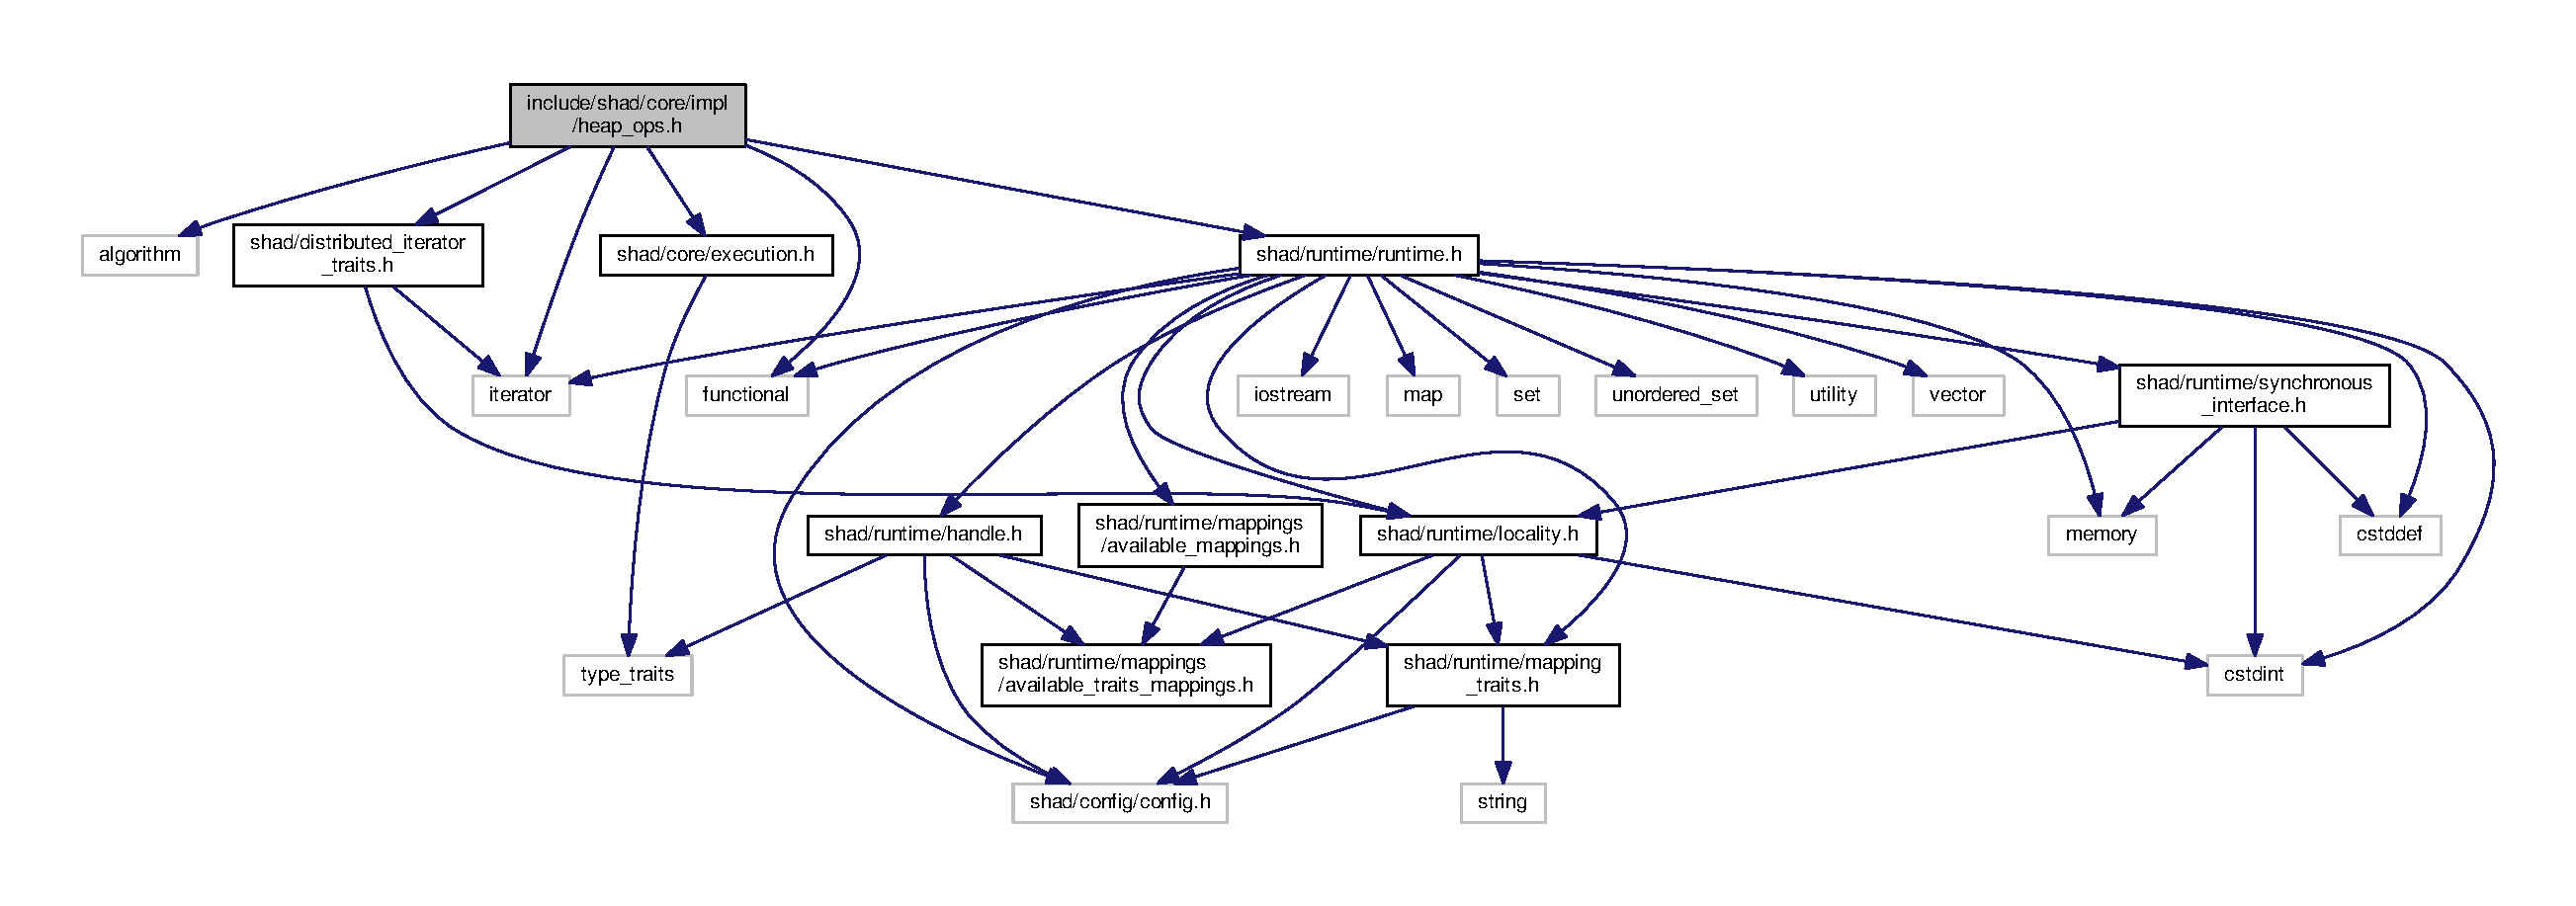
\includegraphics[width=350pt]{heap__ops_8h__incl}
\end{center}
\end{figure}
\subsection*{Namespaces}
\begin{DoxyCompactItemize}
\item 
\hyperlink{namespaceshad}{shad}
\end{DoxyCompactItemize}

\hypertarget{impl__patterns_8h}{\section{include/shad/core/impl/impl\-\_\-patterns.h File Reference}
\label{impl__patterns_8h}\index{include/shad/core/impl/impl\-\_\-patterns.\-h@{include/shad/core/impl/impl\-\_\-patterns.\-h}}
}
{\ttfamily \#include $<$cstddef$>$}\\*
{\ttfamily \#include $<$iterator$>$}\\*
{\ttfamily \#include $<$tuple$>$}\\*
{\ttfamily \#include $<$type\-\_\-traits$>$}\\*
{\ttfamily \#include $<$utility$>$}\\*
{\ttfamily \#include $<$vector$>$}\\*
{\ttfamily \#include \char`\"{}shad/distributed\-\_\-iterator\-\_\-traits.\-h\char`\"{}}\\*
{\ttfamily \#include \char`\"{}shad/runtime/runtime.\-h\char`\"{}}\\*
Include dependency graph for impl\-\_\-patterns.\-h\-:
\nopagebreak
\begin{figure}[H]
\begin{center}
\leavevmode
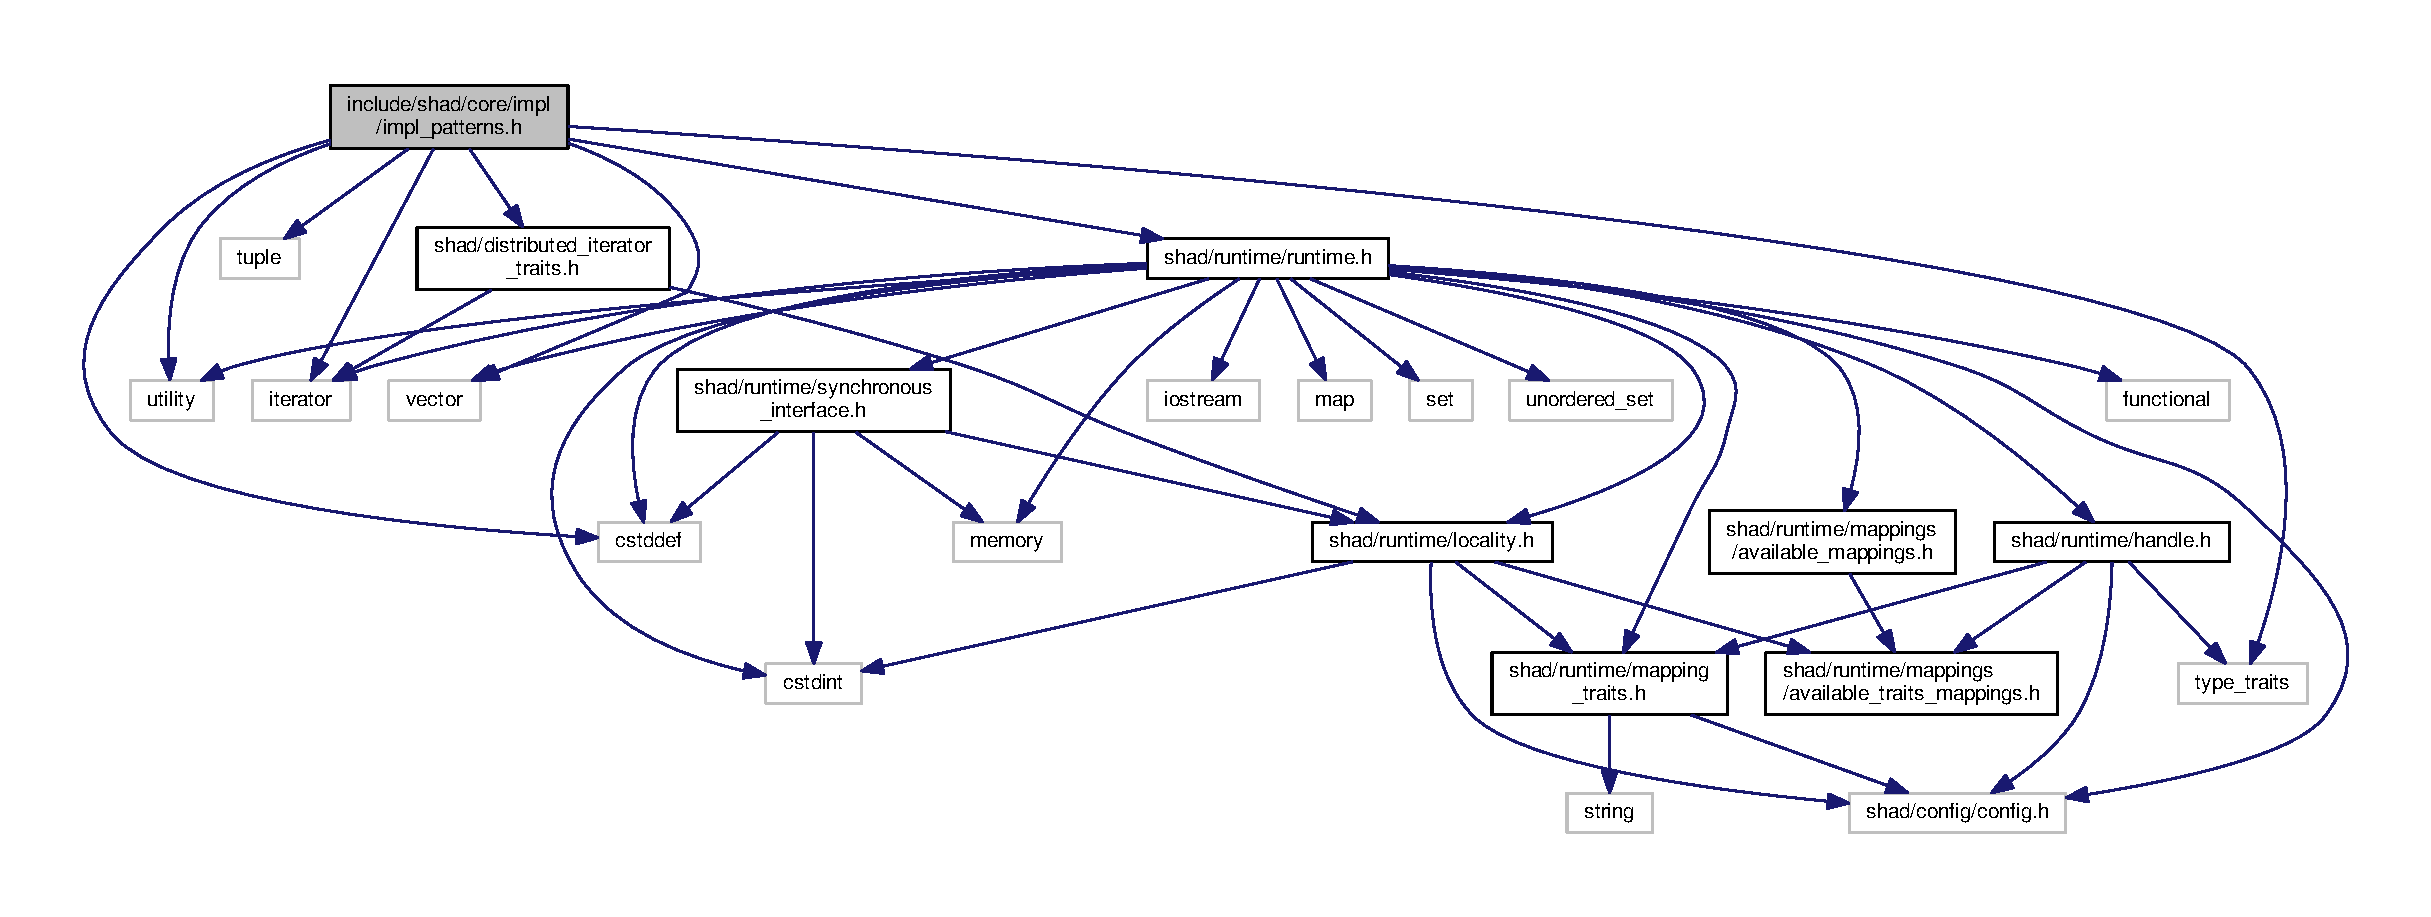
\includegraphics[width=350pt]{impl__patterns_8h__incl}
\end{center}
\end{figure}
This graph shows which files directly or indirectly include this file\-:
\nopagebreak
\begin{figure}[H]
\begin{center}
\leavevmode
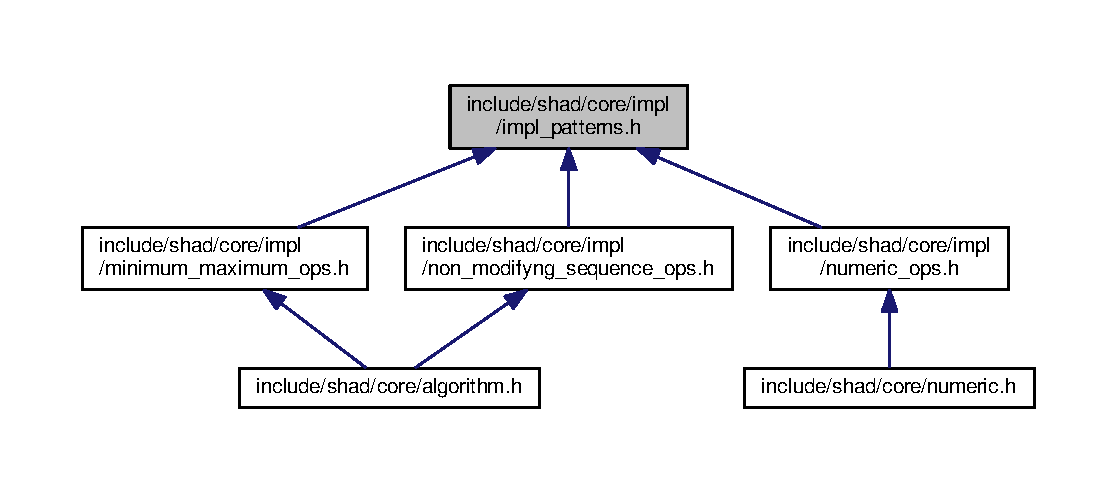
\includegraphics[width=350pt]{impl__patterns_8h__dep__incl}
\end{center}
\end{figure}
\subsection*{Namespaces}
\begin{DoxyCompactItemize}
\item 
\hyperlink{namespaceshad}{shad}
\end{DoxyCompactItemize}

\hypertarget{minimum__maximum__ops_8h}{\section{include/shad/core/impl/minimum\-\_\-maximum\-\_\-ops.h File Reference}
\label{minimum__maximum__ops_8h}\index{include/shad/core/impl/minimum\-\_\-maximum\-\_\-ops.\-h@{include/shad/core/impl/minimum\-\_\-maximum\-\_\-ops.\-h}}
}
{\ttfamily \#include $<$algorithm$>$}\\*
{\ttfamily \#include $<$functional$>$}\\*
{\ttfamily \#include $<$iterator$>$}\\*
{\ttfamily \#include $<$tuple$>$}\\*
{\ttfamily \#include $<$type\-\_\-traits$>$}\\*
{\ttfamily \#include $<$vector$>$}\\*
{\ttfamily \#include \char`\"{}shad/core/execution.\-h\char`\"{}}\\*
{\ttfamily \#include \char`\"{}shad/distributed\-\_\-iterator\-\_\-traits.\-h\char`\"{}}\\*
{\ttfamily \#include \char`\"{}shad/runtime/runtime.\-h\char`\"{}}\\*
{\ttfamily \#include \char`\"{}impl\-\_\-patterns.\-h\char`\"{}}\\*
Include dependency graph for minimum\-\_\-maximum\-\_\-ops.\-h\-:
\nopagebreak
\begin{figure}[H]
\begin{center}
\leavevmode
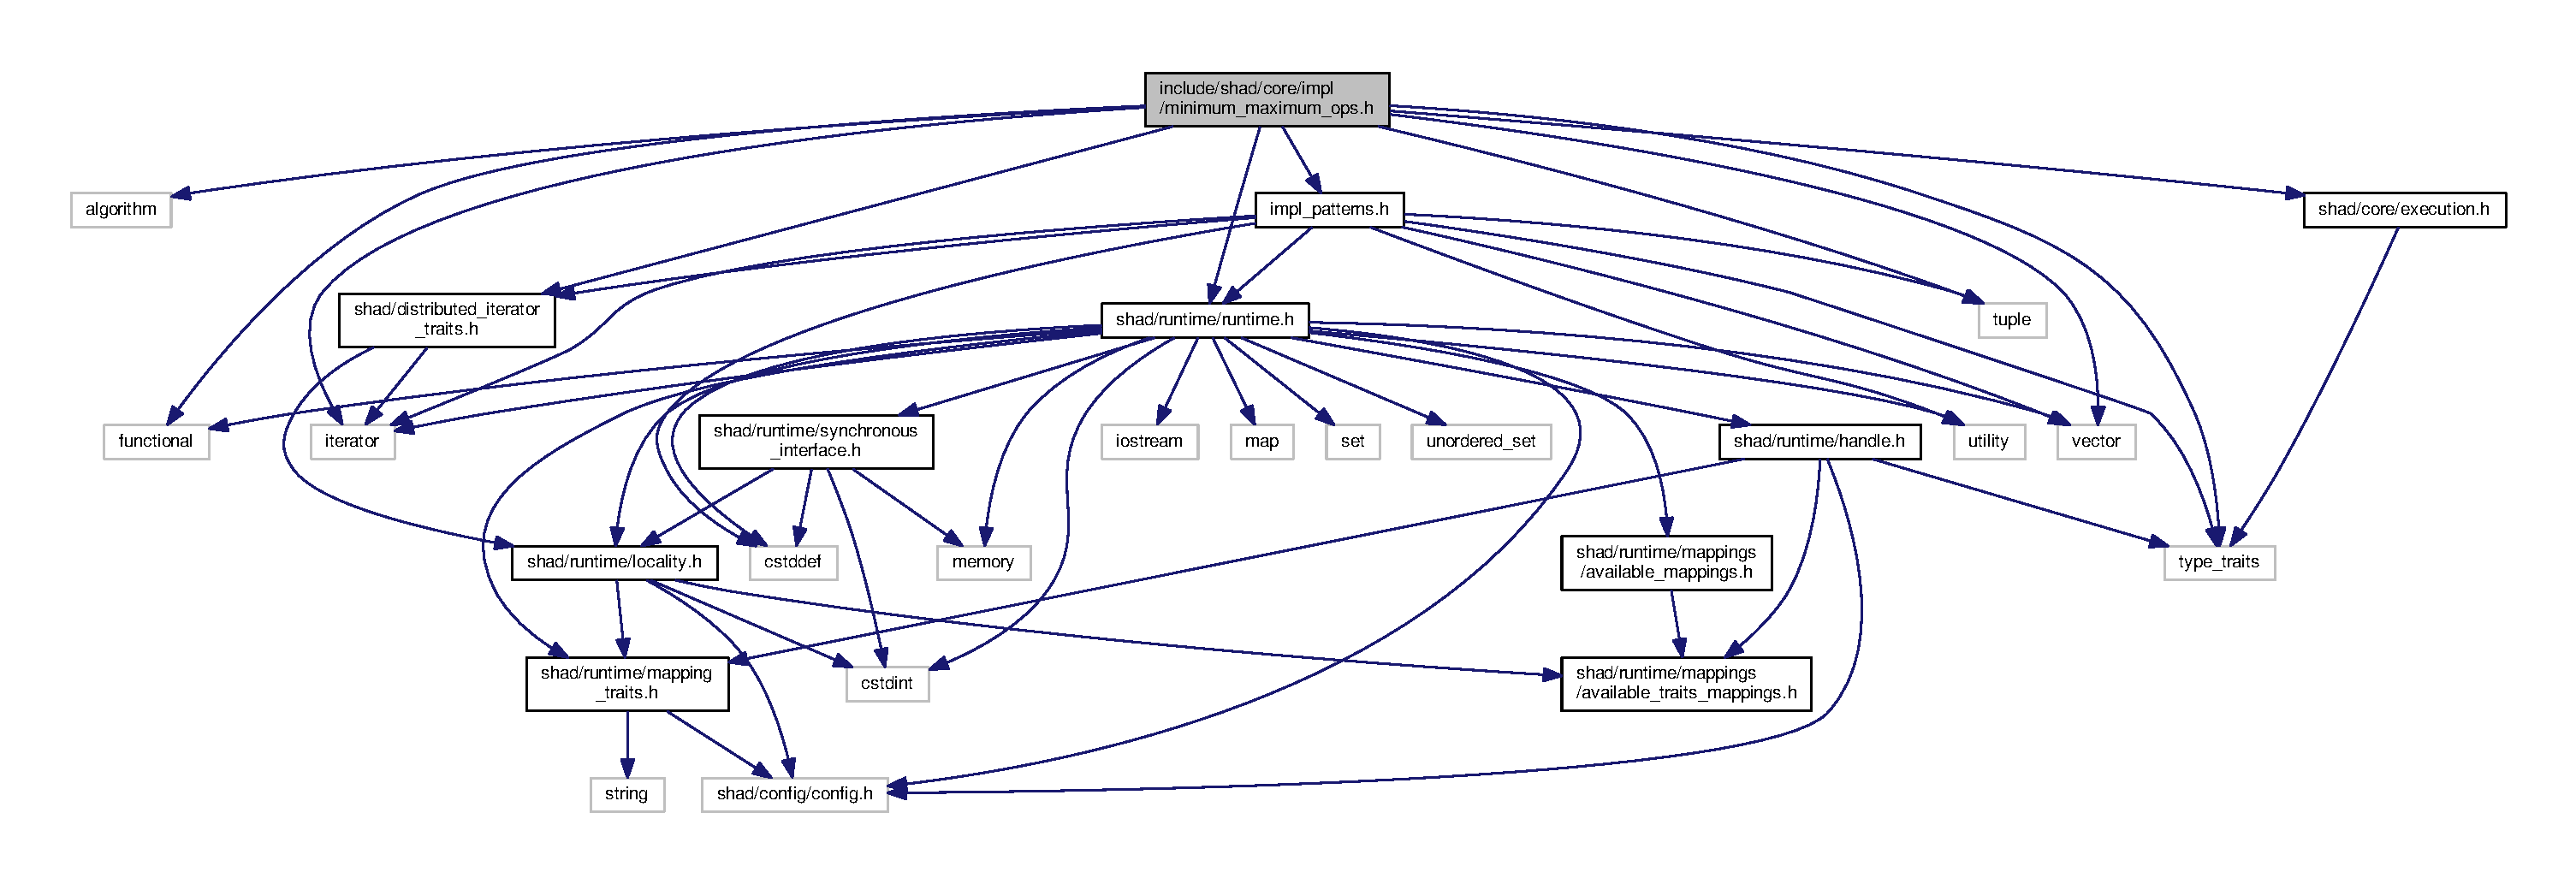
\includegraphics[width=350pt]{minimum__maximum__ops_8h__incl}
\end{center}
\end{figure}
This graph shows which files directly or indirectly include this file\-:
\nopagebreak
\begin{figure}[H]
\begin{center}
\leavevmode
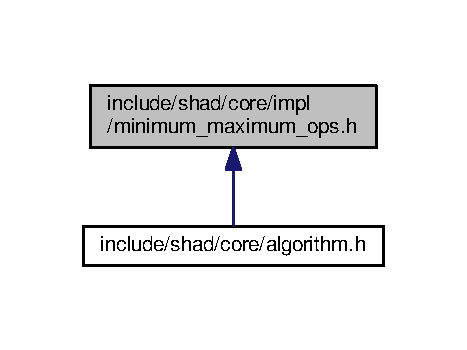
\includegraphics[width=224pt]{minimum__maximum__ops_8h__dep__incl}
\end{center}
\end{figure}
\subsection*{Namespaces}
\begin{DoxyCompactItemize}
\item 
\hyperlink{namespaceshad}{shad}
\end{DoxyCompactItemize}

\hypertarget{modifyng__sequence__ops_8h}{\section{include/shad/core/impl/modifyng\-\_\-sequence\-\_\-ops.h File Reference}
\label{modifyng__sequence__ops_8h}\index{include/shad/core/impl/modifyng\-\_\-sequence\-\_\-ops.\-h@{include/shad/core/impl/modifyng\-\_\-sequence\-\_\-ops.\-h}}
}
{\ttfamily \#include $<$algorithm$>$}\\*
{\ttfamily \#include $<$cstring$>$}\\*
{\ttfamily \#include $<$functional$>$}\\*
{\ttfamily \#include $<$iterator$>$}\\*
{\ttfamily \#include $<$tuple$>$}\\*
{\ttfamily \#include \char`\"{}shad/core/execution.\-h\char`\"{}}\\*
{\ttfamily \#include \char`\"{}shad/core/impl/utils.\-h\char`\"{}}\\*
{\ttfamily \#include \char`\"{}shad/distributed\-\_\-iterator\-\_\-traits.\-h\char`\"{}}\\*
{\ttfamily \#include \char`\"{}shad/runtime/runtime.\-h\char`\"{}}\\*
Include dependency graph for modifyng\-\_\-sequence\-\_\-ops.\-h\-:
\nopagebreak
\begin{figure}[H]
\begin{center}
\leavevmode
\includegraphics[width=350pt]{modifyng__sequence__ops_8h__incl}
\end{center}
\end{figure}
This graph shows which files directly or indirectly include this file\-:
\nopagebreak
\begin{figure}[H]
\begin{center}
\leavevmode
\includegraphics[width=224pt]{modifyng__sequence__ops_8h__dep__incl}
\end{center}
\end{figure}
\subsection*{Namespaces}
\begin{DoxyCompactItemize}
\item 
\hyperlink{namespaceshad}{shad}
\end{DoxyCompactItemize}

\hypertarget{non__modifyng__sequence__ops_8h}{\section{include/shad/core/impl/non\-\_\-modifyng\-\_\-sequence\-\_\-ops.h File Reference}
\label{non__modifyng__sequence__ops_8h}\index{include/shad/core/impl/non\-\_\-modifyng\-\_\-sequence\-\_\-ops.\-h@{include/shad/core/impl/non\-\_\-modifyng\-\_\-sequence\-\_\-ops.\-h}}
}
{\ttfamily \#include $<$algorithm$>$}\\*
{\ttfamily \#include $<$cstddef$>$}\\*
{\ttfamily \#include $<$cstdint$>$}\\*
{\ttfamily \#include $<$functional$>$}\\*
{\ttfamily \#include $<$iterator$>$}\\*
{\ttfamily \#include \char`\"{}shad/core/execution.\-h\char`\"{}}\\*
{\ttfamily \#include \char`\"{}shad/distributed\-\_\-iterator\-\_\-traits.\-h\char`\"{}}\\*
{\ttfamily \#include \char`\"{}shad/runtime/runtime.\-h\char`\"{}}\\*
{\ttfamily \#include \char`\"{}impl\-\_\-patterns.\-h\char`\"{}}\\*
Include dependency graph for non\-\_\-modifyng\-\_\-sequence\-\_\-ops.\-h\-:
\nopagebreak
\begin{figure}[H]
\begin{center}
\leavevmode
\includegraphics[width=350pt]{non__modifyng__sequence__ops_8h__incl}
\end{center}
\end{figure}
This graph shows which files directly or indirectly include this file\-:
\nopagebreak
\begin{figure}[H]
\begin{center}
\leavevmode
\includegraphics[width=236pt]{non__modifyng__sequence__ops_8h__dep__incl}
\end{center}
\end{figure}
\subsection*{Namespaces}
\begin{DoxyCompactItemize}
\item 
\hyperlink{namespaceshad}{shad}
\end{DoxyCompactItemize}

\hypertarget{numeric__ops_8h}{\section{include/shad/core/impl/numeric\-\_\-ops.h File Reference}
\label{numeric__ops_8h}\index{include/shad/core/impl/numeric\-\_\-ops.\-h@{include/shad/core/impl/numeric\-\_\-ops.\-h}}
}
{\ttfamily \#include $<$algorithm$>$}\\*
{\ttfamily \#include $<$functional$>$}\\*
{\ttfamily \#include $<$iterator$>$}\\*
{\ttfamily \#include $<$numeric$>$}\\*
{\ttfamily \#include \char`\"{}shad/core/execution.\-h\char`\"{}}\\*
{\ttfamily \#include \char`\"{}shad/distributed\-\_\-iterator\-\_\-traits.\-h\char`\"{}}\\*
{\ttfamily \#include \char`\"{}shad/runtime/runtime.\-h\char`\"{}}\\*
{\ttfamily \#include \char`\"{}impl\-\_\-patterns.\-h\char`\"{}}\\*
Include dependency graph for numeric\-\_\-ops.\-h\-:
\nopagebreak
\begin{figure}[H]
\begin{center}
\leavevmode
\includegraphics[width=350pt]{numeric__ops_8h__incl}
\end{center}
\end{figure}
This graph shows which files directly or indirectly include this file\-:
\nopagebreak
\begin{figure}[H]
\begin{center}
\leavevmode
\includegraphics[width=218pt]{numeric__ops_8h__dep__incl}
\end{center}
\end{figure}
\subsection*{Namespaces}
\begin{DoxyCompactItemize}
\item 
\hyperlink{namespaceshad}{shad}
\end{DoxyCompactItemize}

\hypertarget{ops__on__uninitialized__memory_8h}{\section{include/shad/core/impl/ops\-\_\-on\-\_\-uninitialized\-\_\-memory.h File Reference}
\label{ops__on__uninitialized__memory_8h}\index{include/shad/core/impl/ops\-\_\-on\-\_\-uninitialized\-\_\-memory.\-h@{include/shad/core/impl/ops\-\_\-on\-\_\-uninitialized\-\_\-memory.\-h}}
}
{\ttfamily \#include $<$algorithm$>$}\\*
{\ttfamily \#include $<$functional$>$}\\*
{\ttfamily \#include $<$iterator$>$}\\*
{\ttfamily \#include \char`\"{}shad/core/execution.\-h\char`\"{}}\\*
{\ttfamily \#include \char`\"{}shad/distributed\-\_\-iterator\-\_\-traits.\-h\char`\"{}}\\*
{\ttfamily \#include \char`\"{}shad/runtime/runtime.\-h\char`\"{}}\\*
Include dependency graph for ops\-\_\-on\-\_\-uninitialized\-\_\-memory.\-h\-:
\nopagebreak
\begin{figure}[H]
\begin{center}
\leavevmode
\includegraphics[width=350pt]{ops__on__uninitialized__memory_8h__incl}
\end{center}
\end{figure}
\subsection*{Namespaces}
\begin{DoxyCompactItemize}
\item 
\hyperlink{namespaceshad}{shad}
\end{DoxyCompactItemize}

\hypertarget{other__ops__on__sorted__ranges_8h}{\section{include/shad/core/impl/other\-\_\-ops\-\_\-on\-\_\-sorted\-\_\-ranges.h File Reference}
\label{other__ops__on__sorted__ranges_8h}\index{include/shad/core/impl/other\-\_\-ops\-\_\-on\-\_\-sorted\-\_\-ranges.\-h@{include/shad/core/impl/other\-\_\-ops\-\_\-on\-\_\-sorted\-\_\-ranges.\-h}}
}
{\ttfamily \#include $<$algorithm$>$}\\*
{\ttfamily \#include $<$functional$>$}\\*
{\ttfamily \#include $<$iterator$>$}\\*
{\ttfamily \#include \char`\"{}shad/core/execution.\-h\char`\"{}}\\*
{\ttfamily \#include \char`\"{}shad/distributed\-\_\-iterator\-\_\-traits.\-h\char`\"{}}\\*
{\ttfamily \#include \char`\"{}shad/runtime/runtime.\-h\char`\"{}}\\*
Include dependency graph for other\-\_\-ops\-\_\-on\-\_\-sorted\-\_\-ranges.\-h\-:
\nopagebreak
\begin{figure}[H]
\begin{center}
\leavevmode
\includegraphics[width=350pt]{other__ops__on__sorted__ranges_8h__incl}
\end{center}
\end{figure}
\subsection*{Namespaces}
\begin{DoxyCompactItemize}
\item 
\hyperlink{namespaceshad}{shad}
\end{DoxyCompactItemize}

\hypertarget{partitioning__ops_8h}{\section{include/shad/core/impl/partitioning\-\_\-ops.h File Reference}
\label{partitioning__ops_8h}\index{include/shad/core/impl/partitioning\-\_\-ops.\-h@{include/shad/core/impl/partitioning\-\_\-ops.\-h}}
}
{\ttfamily \#include $<$algorithm$>$}\\*
{\ttfamily \#include $<$functional$>$}\\*
{\ttfamily \#include $<$iterator$>$}\\*
{\ttfamily \#include \char`\"{}shad/core/execution.\-h\char`\"{}}\\*
{\ttfamily \#include \char`\"{}shad/distributed\-\_\-iterator\-\_\-traits.\-h\char`\"{}}\\*
{\ttfamily \#include \char`\"{}shad/runtime/runtime.\-h\char`\"{}}\\*
Include dependency graph for partitioning\-\_\-ops.\-h\-:
\nopagebreak
\begin{figure}[H]
\begin{center}
\leavevmode
\includegraphics[width=350pt]{partitioning__ops_8h__incl}
\end{center}
\end{figure}
\subsection*{Namespaces}
\begin{DoxyCompactItemize}
\item 
\hyperlink{namespaceshad}{shad}
\end{DoxyCompactItemize}

\hypertarget{permutation__ops_8h}{\section{include/shad/core/impl/permutation\-\_\-ops.h File Reference}
\label{permutation__ops_8h}\index{include/shad/core/impl/permutation\-\_\-ops.\-h@{include/shad/core/impl/permutation\-\_\-ops.\-h}}
}
{\ttfamily \#include $<$algorithm$>$}\\*
{\ttfamily \#include $<$functional$>$}\\*
{\ttfamily \#include $<$iterator$>$}\\*
{\ttfamily \#include \char`\"{}shad/core/execution.\-h\char`\"{}}\\*
{\ttfamily \#include \char`\"{}shad/distributed\-\_\-iterator\-\_\-traits.\-h\char`\"{}}\\*
{\ttfamily \#include \char`\"{}shad/runtime/runtime.\-h\char`\"{}}\\*
Include dependency graph for permutation\-\_\-ops.\-h\-:
\nopagebreak
\begin{figure}[H]
\begin{center}
\leavevmode
\includegraphics[width=350pt]{permutation__ops_8h__incl}
\end{center}
\end{figure}
\subsection*{Namespaces}
\begin{DoxyCompactItemize}
\item 
\hyperlink{namespaceshad}{shad}
\end{DoxyCompactItemize}

\hypertarget{set__ops_8h}{\section{include/shad/core/impl/set\-\_\-ops.h File Reference}
\label{set__ops_8h}\index{include/shad/core/impl/set\-\_\-ops.\-h@{include/shad/core/impl/set\-\_\-ops.\-h}}
}
{\ttfamily \#include $<$algorithm$>$}\\*
{\ttfamily \#include $<$functional$>$}\\*
{\ttfamily \#include $<$iterator$>$}\\*
{\ttfamily \#include \char`\"{}shad/core/execution.\-h\char`\"{}}\\*
{\ttfamily \#include \char`\"{}shad/distributed\-\_\-iterator\-\_\-traits.\-h\char`\"{}}\\*
{\ttfamily \#include \char`\"{}shad/runtime/runtime.\-h\char`\"{}}\\*
Include dependency graph for set\-\_\-ops.\-h\-:
\nopagebreak
\begin{figure}[H]
\begin{center}
\leavevmode
\includegraphics[width=350pt]{set__ops_8h__incl}
\end{center}
\end{figure}
\subsection*{Namespaces}
\begin{DoxyCompactItemize}
\item 
\hyperlink{namespaceshad}{shad}
\end{DoxyCompactItemize}

\hypertarget{sorting__ops_8h}{\section{include/shad/core/impl/sorting\-\_\-ops.h File Reference}
\label{sorting__ops_8h}\index{include/shad/core/impl/sorting\-\_\-ops.\-h@{include/shad/core/impl/sorting\-\_\-ops.\-h}}
}
{\ttfamily \#include $<$algorithm$>$}\\*
{\ttfamily \#include $<$functional$>$}\\*
{\ttfamily \#include $<$iterator$>$}\\*
{\ttfamily \#include \char`\"{}shad/core/execution.\-h\char`\"{}}\\*
{\ttfamily \#include \char`\"{}shad/distributed\-\_\-iterator\-\_\-traits.\-h\char`\"{}}\\*
{\ttfamily \#include \char`\"{}shad/runtime/runtime.\-h\char`\"{}}\\*
Include dependency graph for sorting\-\_\-ops.\-h\-:
\nopagebreak
\begin{figure}[H]
\begin{center}
\leavevmode
\includegraphics[width=350pt]{sorting__ops_8h__incl}
\end{center}
\end{figure}
\subsection*{Namespaces}
\begin{DoxyCompactItemize}
\item 
\hyperlink{namespaceshad}{shad}
\end{DoxyCompactItemize}

\hypertarget{utils_8h}{\section{include/shad/core/impl/utils.h File Reference}
\label{utils_8h}\index{include/shad/core/impl/utils.\-h@{include/shad/core/impl/utils.\-h}}
}
{\ttfamily \#include $<$algorithm$>$}\\*
{\ttfamily \#include $<$functional$>$}\\*
{\ttfamily \#include $<$iterator$>$}\\*
{\ttfamily \#include \char`\"{}shad/core/iterator.\-h\char`\"{}}\\*
{\ttfamily \#include \char`\"{}shad/distributed\-\_\-iterator\-\_\-traits.\-h\char`\"{}}\\*
{\ttfamily \#include \char`\"{}shad/runtime/runtime.\-h\char`\"{}}\\*
Include dependency graph for utils.\-h\-:
\nopagebreak
\begin{figure}[H]
\begin{center}
\leavevmode
\includegraphics[width=350pt]{utils_8h__incl}
\end{center}
\end{figure}
This graph shows which files directly or indirectly include this file\-:
\nopagebreak
\begin{figure}[H]
\begin{center}
\leavevmode
\includegraphics[width=224pt]{utils_8h__dep__incl}
\end{center}
\end{figure}
\subsection*{Namespaces}
\begin{DoxyCompactItemize}
\item 
\hyperlink{namespaceshad}{shad}
\end{DoxyCompactItemize}

\hypertarget{iterator_8h}{\section{include/shad/core/iterator.h File Reference}
\label{iterator_8h}\index{include/shad/core/iterator.\-h@{include/shad/core/iterator.\-h}}
}
{\ttfamily \#include $<$iterator$>$}\\*
{\ttfamily \#include $<$memory$>$}\\*
Include dependency graph for iterator.\-h\-:
\nopagebreak
\begin{figure}[H]
\begin{center}
\leavevmode
\includegraphics[width=214pt]{iterator_8h__incl}
\end{center}
\end{figure}
This graph shows which files directly or indirectly include this file\-:
\nopagebreak
\begin{figure}[H]
\begin{center}
\leavevmode
\includegraphics[width=350pt]{iterator_8h__dep__incl}
\end{center}
\end{figure}
\subsection*{Classes}
\begin{DoxyCompactItemize}
\item 
class \hyperlink{classshad_1_1buffered__insert__iterator}{shad\-::buffered\-\_\-insert\-\_\-iterator$<$ Container $>$}
\begin{DoxyCompactList}\small\item\em Buffered insert iterator. \end{DoxyCompactList}\end{DoxyCompactItemize}
\subsection*{Namespaces}
\begin{DoxyCompactItemize}
\item 
\hyperlink{namespaceshad}{shad}
\end{DoxyCompactItemize}

\hypertarget{numeric_8h}{\section{include/shad/core/numeric.h File Reference}
\label{numeric_8h}\index{include/shad/core/numeric.\-h@{include/shad/core/numeric.\-h}}
}
{\ttfamily \#include $<$functional$>$}\\*
{\ttfamily \#include $<$iterator$>$}\\*
{\ttfamily \#include $<$tuple$>$}\\*
{\ttfamily \#include $<$utility$>$}\\*
{\ttfamily \#include $<$vector$>$}\\*
{\ttfamily \#include \char`\"{}shad/core/execution.\-h\char`\"{}}\\*
{\ttfamily \#include \char`\"{}shad/core/impl/numeric\-\_\-ops.\-h\char`\"{}}\\*
{\ttfamily \#include \char`\"{}shad/distributed\-\_\-iterator\-\_\-traits.\-h\char`\"{}}\\*
{\ttfamily \#include \char`\"{}shad/runtime/runtime.\-h\char`\"{}}\\*
Include dependency graph for numeric.\-h\-:
\nopagebreak
\begin{figure}[H]
\begin{center}
\leavevmode
\includegraphics[width=350pt]{numeric_8h__incl}
\end{center}
\end{figure}
\subsection*{Namespaces}
\begin{DoxyCompactItemize}
\item 
\hyperlink{namespaceshad}{shad}
\end{DoxyCompactItemize}
\subsection*{Functions}
\begin{DoxyCompactItemize}
\item 
{\footnotesize template$<$class Forward\-Iterator , class T $>$ }\\void \hyperlink{namespaceshad_a1406d52ae9f56d5b4a160d37b2b20f3a}{shad\-::iota} (Forward\-Iterator first, Forward\-Iterator last, T value)
\item 
{\footnotesize template$<$class Input\-It , class T , class Binary\-Operation $>$ }\\T \hyperlink{namespaceshad_a79535b2ad05d27266485f8e299b776cd}{shad\-::accumulate} (Input\-It first, Input\-It last, T init, Binary\-Operation op)
\item 
{\footnotesize template$<$class Input\-It , class T $>$ }\\T \hyperlink{namespaceshad_a7286bb0b681bec70602b31083a0b0680}{shad\-::accumulate} (Input\-It first, Input\-It last, T init)
\item 
{\footnotesize template$<$class Input\-It1 , class Input\-It2 , class T $>$ }\\T \hyperlink{namespaceshad_ae17dfe23117ed2d68100db112d13d5e2}{shad\-::inner\-\_\-product} (Input\-It1 first1, Input\-It1 last1, Input\-It2 first2, T init)
\item 
{\footnotesize template$<$class Input\-It1 , class Input\-It2 , class T , class Binary\-Operation1 , class Binary\-Operation2 $>$ }\\T \hyperlink{namespaceshad_a9e35d019afa66a7d241f01c4c28a5c14}{shad\-::inner\-\_\-product} (Input\-It1 first1, Input\-It1 last1, Input\-It2 first2, T init, Binary\-Operation1 op1, Binary\-Operation2 op2)
\item 
{\footnotesize template$<$class Input\-It , class Output\-It $>$ }\\Output\-It \hyperlink{namespaceshad_a740dc92192ebb80d0651a62c31ad92ec}{shad\-::adjacent\-\_\-difference} (Input\-It first, Input\-It last, Output\-It d\-\_\-first)
\item 
{\footnotesize template$<$typename Execution\-Policy , class Input\-It , class Output\-It $>$ }\\std\-::enable\-\_\-if\-\_\-t\\*
$<$ \hyperlink{structshad_1_1is__execution__policy}{shad\-::is\-\_\-execution\-\_\-policy}\\*
$<$ Execution\-Policy $>$\-::value, \\*
Output\-It $>$ \hyperlink{namespaceshad_affad70e4283f19271fe3ab0ea3ce1b90}{shad\-::adjacent\-\_\-difference} (Execution\-Policy \&\&policy, Input\-It first, Input\-It last, Output\-It d\-\_\-first)
\item 
{\footnotesize template$<$class Input\-It , class Output\-It , class Binary\-Operation $>$ }\\std\-::enable\-\_\-if\-\_\-t\\*
$<$!\hyperlink{structshad_1_1is__execution__policy}{shad\-::is\-\_\-execution\-\_\-policy}\\*
$<$ Input\-It $>$\-::value, Output\-It $>$ \hyperlink{namespaceshad_ac72a7771f9b490b5948c84da221e9a83}{shad\-::adjacent\-\_\-difference} (Input\-It first, Input\-It last, Output\-It d\-\_\-first, Binary\-Operation op)
\item 
{\footnotesize template$<$typename Execution\-Policy , class Input\-It , class Output\-It , class Binary\-Operation $>$ }\\Output\-It \hyperlink{namespaceshad_a390a66f6af57d674bfcd5aced6b69a9d}{shad\-::adjacent\-\_\-difference} (Execution\-Policy \&\&policy, Input\-It first, Input\-It last, Output\-It d\-\_\-first, Binary\-Operation op)
\item 
{\footnotesize template$<$class Input\-It , class Output\-It $>$ }\\Output\-It \hyperlink{namespaceshad_a08d8882161e132a6fb3f9253b9a3bdef}{shad\-::partial\-\_\-sum} (Input\-It first, Input\-It last, Output\-It d\-\_\-first)
\item 
{\footnotesize template$<$class Input\-It , class Output\-It , class Binary\-Operation $>$ }\\Output\-It \hyperlink{namespaceshad_a82089f3b0373f5062395613e51d16fa3}{shad\-::partial\-\_\-sum} (Input\-It first, Input\-It last, Output\-It d\-\_\-first, Binary\-Operation op)
\item 
{\footnotesize template$<$class Execution\-Policy , class Forward\-It , class T , class Binary\-Op $>$ }\\T \hyperlink{namespaceshad_a23bc7c39dc6aa69f526570d07967a185}{shad\-::reduce} (Execution\-Policy \&\&policy, Forward\-It first, Forward\-It last, T init, Binary\-Op binary\-\_\-op)
\item 
{\footnotesize template$<$class Input\-It $>$ }\\std\-::iterator\-\_\-traits$<$ Input\-It $>$\\*
\-::value\-\_\-type \hyperlink{namespaceshad_a0cb65c2ad084f15e5fd33058445b7f10}{shad\-::reduce} (Input\-It first, Input\-It last)
\item 
{\footnotesize template$<$class Execution\-Policy , class Forward\-It $>$ }\\std\-::enable\-\_\-if\-\_\-t\\*
$<$ \hyperlink{structshad_1_1is__execution__policy}{shad\-::is\-\_\-execution\-\_\-policy}\\*
$<$ Execution\-Policy $>$\-::value, \\*
typename std\-::iterator\-\_\-traits\\*
$<$ Forward\-It $>$\-::value\-\_\-type $>$ \hyperlink{namespaceshad_a329ef698d7c8b55b8b967ad07e9bf84d}{shad\-::reduce} (Execution\-Policy \&\&policy, Forward\-It first, Forward\-It last)
\item 
{\footnotesize template$<$class Input\-It , class T $>$ }\\std\-::enable\-\_\-if\-\_\-t\\*
$<$!\hyperlink{structshad_1_1is__execution__policy}{shad\-::is\-\_\-execution\-\_\-policy}\\*
$<$ Input\-It $>$\-::value, T $>$ \hyperlink{namespaceshad_aea9e6912fe7e3a494de8b7eaad2fd345}{shad\-::reduce} (Input\-It first, Input\-It last, T init)
\item 
{\footnotesize template$<$class Execution\-Policy , class Forward\-It , class T $>$ }\\std\-::enable\-\_\-if\-\_\-t\\*
$<$ \hyperlink{structshad_1_1is__execution__policy}{shad\-::is\-\_\-execution\-\_\-policy}\\*
$<$ Execution\-Policy $>$\-::value, T $>$ \hyperlink{namespaceshad_a047e9c9a109948515a14306d4a169893}{shad\-::reduce} (Execution\-Policy \&\&policy, Forward\-It first, Forward\-It last, T init)
\item 
{\footnotesize template$<$class Input\-It , class T , class Binary\-Op $>$ }\\std\-::enable\-\_\-if\-\_\-t\\*
$<$!\hyperlink{structshad_1_1is__execution__policy}{shad\-::is\-\_\-execution\-\_\-policy}\\*
$<$ Input\-It $>$\-::value, T $>$ \hyperlink{namespaceshad_a2807d313b1e6586657c742ae2b4c132d}{shad\-::reduce} (Input\-It first, Input\-It last, T init, Binary\-Op binary\-\_\-op)
\item 
{\footnotesize template$<$class Input\-It , class Output\-It , class T $>$ }\\Output\-It \hyperlink{namespaceshad_af0252dc307b8ba0b96885c00e8871bbc}{shad\-::exclusive\-\_\-scan} (Input\-It first, Input\-It last, Output\-It d\-\_\-first, T init)
\item 
{\footnotesize template$<$class Execution\-Policy , class Forward\-It1 , class Forward\-It2 , class T $>$ }\\std\-::enable\-\_\-if\-\_\-t\\*
$<$ \hyperlink{structshad_1_1is__execution__policy}{shad\-::is\-\_\-execution\-\_\-policy}\\*
$<$ Execution\-Policy $>$\-::value, \\*
Forward\-It2 $>$ \hyperlink{namespaceshad_a04c9040a1562793e895edaf3517dcfd6}{shad\-::exclusive\-\_\-scan} (Execution\-Policy \&\&policy, Forward\-It1 first, Forward\-It1 last, Forward\-It2 d\-\_\-first, T init)
\item 
{\footnotesize template$<$class Input\-It , class Output\-It , class T , class Binary\-Operation $>$ }\\std\-::enable\-\_\-if\-\_\-t\\*
$<$!\hyperlink{structshad_1_1is__execution__policy}{shad\-::is\-\_\-execution\-\_\-policy}\\*
$<$ Input\-It $>$\-::value, Output\-It $>$ \hyperlink{namespaceshad_a3c4542507eba2afe28bb5d8af386b76d}{shad\-::exclusive\-\_\-scan} (Input\-It first, Input\-It last, Output\-It d\-\_\-first, T init, Binary\-Operation binary\-\_\-op)
\item 
{\footnotesize template$<$class Execution\-Policy , class Forward\-It1 , class Forward\-It2 , class T , class Binary\-Operation $>$ }\\Forward\-It2 \hyperlink{namespaceshad_af1776fbb5971b5b37331938fa9f55e09}{shad\-::exclusive\-\_\-scan} (Execution\-Policy \&\&policy, Forward\-It1 first, Forward\-It1 last, Forward\-It2 d\-\_\-first, T init, Binary\-Operation binary\-\_\-op)
\item 
{\footnotesize template$<$class Input\-It , class Output\-It $>$ }\\Output\-It \hyperlink{namespaceshad_a2854c58c1b96a1d20320f22a34bc2231}{shad\-::inclusive\-\_\-scan} (Input\-It first, Input\-It last, Output\-It d\-\_\-first)
\item 
{\footnotesize template$<$class Execution\-Policy , class Forward\-It1 , class Forward\-It2 $>$ }\\std\-::enable\-\_\-if\-\_\-t\\*
$<$ \hyperlink{structshad_1_1is__execution__policy}{shad\-::is\-\_\-execution\-\_\-policy}\\*
$<$ Execution\-Policy $>$\-::value, \\*
Forward\-It2 $>$ \hyperlink{namespaceshad_a1d3a1d24cc9d681bd236220c3db36a4b}{shad\-::inclusive\-\_\-scan} (Execution\-Policy \&\&policy, Forward\-It1 first, Forward\-It1 last, Forward\-It2 d\-\_\-first)
\item 
{\footnotesize template$<$class Input\-It , class Output\-It , class Binary\-Operation $>$ }\\std\-::enable\-\_\-if\-\_\-t\\*
$<$!\hyperlink{structshad_1_1is__execution__policy}{shad\-::is\-\_\-execution\-\_\-policy}\\*
$<$ Input\-It $>$\-::value, Output\-It $>$ \hyperlink{namespaceshad_ab2f0bce9d14c5ec29670dbbcae4a7e58}{shad\-::inclusive\-\_\-scan} (Input\-It first, Input\-It last, Output\-It d\-\_\-first, Binary\-Operation binary\-\_\-op)
\item 
{\footnotesize template$<$class Execution\-Policy , class Forward\-It1 , class Forward\-It2 , class Binary\-Operation $>$ }\\std\-::enable\-\_\-if\-\_\-t\\*
$<$ \hyperlink{structshad_1_1is__execution__policy}{shad\-::is\-\_\-execution\-\_\-policy}\\*
$<$ Execution\-Policy $>$\-::value, \\*
Forward\-It2 $>$ \hyperlink{namespaceshad_adc86ffac5f28d6798c40434c5017d86f}{shad\-::inclusive\-\_\-scan} (Execution\-Policy \&\&policy, Forward\-It1 first, Forward\-It1 last, Forward\-It2 d\-\_\-first, Binary\-Operation binary\-\_\-op)
\item 
{\footnotesize template$<$class Input\-It , class Output\-It , class Binary\-Operation , class T $>$ }\\std\-::enable\-\_\-if\-\_\-t\\*
$<$!\hyperlink{structshad_1_1is__execution__policy}{shad\-::is\-\_\-execution\-\_\-policy}\\*
$<$ Input\-It $>$\-::value, Output\-It $>$ \hyperlink{namespaceshad_a3a46378a583f1c96000caa42e640ab5c}{shad\-::inclusive\-\_\-scan} (Input\-It first, Input\-It last, Output\-It d\-\_\-first, Binary\-Operation binary\-\_\-op, T init)
\item 
{\footnotesize template$<$class Execution\-Policy , class Forward\-It1 , class Forward\-It2 , class Binary\-Operation , class T $>$ }\\Forward\-It2 \hyperlink{namespaceshad_ac268ceb6647308bdfa9a510f346cc560}{shad\-::inclusive\-\_\-scan} (Execution\-Policy \&\&policy, Forward\-It1 first, Forward\-It1 last, Forward\-It2 d\-\_\-first, Binary\-Operation binary\-\_\-op, T init)
\item 
{\footnotesize template$<$class Execution\-Policy , class Forward\-It , class T , class Binary\-Op , class Unary\-Op $>$ }\\std\-::enable\-\_\-if\-\_\-t\\*
$<$ \hyperlink{structshad_1_1is__execution__policy}{shad\-::is\-\_\-execution\-\_\-policy}\\*
$<$ Execution\-Policy $>$\-::value, T $>$ \hyperlink{namespaceshad_a45c6b8c67b4d583819c334dc29a969b1}{shad\-::transform\-\_\-reduce} (Execution\-Policy \&\&policy, Forward\-It first, Forward\-It last, T init, Binary\-Op binary\-\_\-op, Unary\-Op unary\-\_\-op)
\item 
{\footnotesize template$<$class Execution\-Policy , class Forward\-It1 , class Forward\-It2 , class T , class Binary\-Op1 , class Binary\-Op2 $>$ }\\T \hyperlink{namespaceshad_a9ada8d6b6cb63fd3b5b459ff608b5027}{shad\-::transform\-\_\-reduce} (Execution\-Policy \&\&policy, Forward\-It1 first1, Forward\-It1 last1, Forward\-It2 first2, T init, Binary\-Op1 binary\-\_\-op1, Binary\-Op2 binary\-\_\-op2)
\item 
{\footnotesize template$<$class Input\-It1 , class Input\-It2 , class T $>$ }\\T \hyperlink{namespaceshad_a9fb77cb6187be97748be38c5632a406c}{shad\-::transform\-\_\-reduce} (Input\-It1 first1, Input\-It1 last1, Input\-It2 first2, T init)
\item 
{\footnotesize template$<$class Input\-It1 , class Input\-It2 , class T , class Binary\-Op1 , class Binary\-Op2 $>$ }\\std\-::enable\-\_\-if\-\_\-t\\*
$<$!\hyperlink{structshad_1_1is__execution__policy}{shad\-::is\-\_\-execution\-\_\-policy}\\*
$<$ Input\-It1 $>$\-::value, T $>$ \hyperlink{namespaceshad_a6764e68a376e02ec492499b12eac8dc1}{shad\-::transform\-\_\-reduce} (Input\-It1 first1, Input\-It1 last1, Input\-It2 first2, T init, Binary\-Op1 binary\-\_\-op1, Binary\-Op2 binary\-\_\-op2)
\item 
{\footnotesize template$<$class Input\-It , class T , class Binary\-Op , class Unary\-Op $>$ }\\std\-::enable\-\_\-if\-\_\-t\\*
$<$!\hyperlink{structshad_1_1is__execution__policy}{shad\-::is\-\_\-execution\-\_\-policy}\\*
$<$ Input\-It $>$\-::value, T $>$ \hyperlink{namespaceshad_a68e4deac86c665ff2d3d3550c7042331}{shad\-::transform\-\_\-reduce} (Input\-It first, Input\-It last, T init, Binary\-Op binop, Unary\-Op unary\-\_\-op)
\item 
{\footnotesize template$<$class Execution\-Policy , class Forward\-It1 , class Forward\-It2 , class T $>$ }\\std\-::enable\-\_\-if\-\_\-t\\*
$<$ \hyperlink{structshad_1_1is__execution__policy}{shad\-::is\-\_\-execution\-\_\-policy}\\*
$<$ Execution\-Policy $>$\-::value, T $>$ \hyperlink{namespaceshad_a1de0e51e5616aabd05a68412086358ae}{shad\-::transform\-\_\-reduce} (Execution\-Policy \&\&policy, Forward\-It1 first1, Forward\-It1 last1, Forward\-It2 first2, T init)
\item 
{\footnotesize template$<$class Input\-It , class Output\-It , class T , class Binary\-Operation , class Unary\-Operation $>$ }\\Output\-It \hyperlink{namespaceshad_a58f5206d294f2437782ed7f197eb1d0d}{shad\-::transform\-\_\-exclusive\-\_\-scan} (Input\-It first, Input\-It last, Output\-It d\-\_\-first, T init, Binary\-Operation binary\-\_\-op, Unary\-Operation unary\-\_\-op)
\item 
{\footnotesize template$<$class Execution\-Policy , class Forward\-It1 , class Forward\-It2 , class T , class Binary\-Operation , class Unary\-Operation $>$ }\\Forward\-It2 \hyperlink{namespaceshad_a1ad8ba4e807e353d19cbe7f118914856}{shad\-::transform\-\_\-exclusive\-\_\-scan} (Execution\-Policy \&\&policy, Forward\-It1 first, Forward\-It1 last, Forward\-It2 d\-\_\-first, T init, Binary\-Operation binary\-\_\-op, Unary\-Operation unary\-\_\-op)
\item 
{\footnotesize template$<$class Input\-It , class Output\-It , class Binary\-Operation , class Unary\-Operation $>$ }\\Output\-It \hyperlink{namespaceshad_abae2714cc427e081f0f399648d5cfdef}{shad\-::transform\-\_\-inclusive\-\_\-scan} (Input\-It first, Input\-It last, Output\-It d\-\_\-first, Binary\-Operation binary\-\_\-op, Unary\-Operation unary\-\_\-op)
\item 
{\footnotesize template$<$class Execution\-Policy , class Forward\-It1 , class Forward\-It2 , class Binary\-Operation , class Unary\-Operation $>$ }\\std\-::enable\-\_\-if\-\_\-t\\*
$<$ \hyperlink{structshad_1_1is__execution__policy}{shad\-::is\-\_\-execution\-\_\-policy}\\*
$<$ Execution\-Policy $>$\-::value, \\*
Forward\-It2 $>$ \hyperlink{namespaceshad_a0d3e58f6b91d06bf7d3f46e7d2e478bc}{shad\-::transform\-\_\-inclusive\-\_\-scan} (Execution\-Policy \&\&policy, Forward\-It1 first, Forward\-It1 last, Forward\-It2 d\-\_\-first, Binary\-Operation binary\-\_\-op, Unary\-Operation unary\-\_\-op)
\item 
{\footnotesize template$<$class Input\-It , class Output\-It , class Binary\-Operation , class Unary\-Operation , class T $>$ }\\std\-::enable\-\_\-if\-\_\-t\\*
$<$!\hyperlink{structshad_1_1is__execution__policy}{shad\-::is\-\_\-execution\-\_\-policy}\\*
$<$ Input\-It $>$\-::value, Output\-It $>$ \hyperlink{namespaceshad_aa7967d1c57c2457d65e5a8dc09b98c0e}{shad\-::transform\-\_\-inclusive\-\_\-scan} (Input\-It first, Input\-It last, Output\-It d\-\_\-first, Binary\-Operation binary\-\_\-op, Unary\-Operation unary\-\_\-op, T init)
\item 
{\footnotesize template$<$class Execution\-Policy , class Forward\-It1 , class Forward\-It2 , class Binary\-Operation , class Unary\-Operation , class T $>$ }\\Forward\-It2 \hyperlink{namespaceshad_a7731b3ca77801af3286844f6db55364c}{shad\-::transform\-\_\-inclusive\-\_\-scan} (Execution\-Policy \&\&policy, Forward\-It1 first, Forward\-It1 last, Forward\-It2 d\-\_\-first, Binary\-Operation binary\-\_\-op, Unary\-Operation unary\-\_\-op, T init)
\end{DoxyCompactItemize}

\hypertarget{type__traits_8h}{\section{include/shad/core/type\-\_\-traits.h File Reference}
\label{type__traits_8h}\index{include/shad/core/type\-\_\-traits.\-h@{include/shad/core/type\-\_\-traits.\-h}}
}
{\ttfamily \#include $<$functional$>$}\\*
{\ttfamily \#include $<$type\-\_\-traits$>$}\\*
Include dependency graph for type\-\_\-traits.\-h\-:
\nopagebreak
\begin{figure}[H]
\begin{center}
\leavevmode
\includegraphics[width=219pt]{type__traits_8h__incl}
\end{center}
\end{figure}
This graph shows which files directly or indirectly include this file\-:
\nopagebreak
\begin{figure}[H]
\begin{center}
\leavevmode
\includegraphics[width=350pt]{type__traits_8h__dep__incl}
\end{center}
\end{figure}
\subsection*{Classes}
\begin{DoxyCompactItemize}
\item 
struct \hyperlink{structshad_1_1is__std__hashable}{shad\-::is\-\_\-std\-\_\-hashable$<$ T $>$}
\end{DoxyCompactItemize}
\subsection*{Namespaces}
\begin{DoxyCompactItemize}
\item 
\hyperlink{namespaceshad}{shad}
\end{DoxyCompactItemize}

\hypertarget{unordered__map_8h}{\section{include/shad/core/unordered\-\_\-map.h File Reference}
\label{unordered__map_8h}\index{include/shad/core/unordered\-\_\-map.\-h@{include/shad/core/unordered\-\_\-map.\-h}}
}
{\ttfamily \#include \char`\"{}shad/core/iterator.\-h\char`\"{}}\\*
{\ttfamily \#include \char`\"{}shad/data\-\_\-structures/compare\-\_\-and\-\_\-hash\-\_\-utils.\-h\char`\"{}}\\*
{\ttfamily \#include \char`\"{}shad/data\-\_\-structures/hashmap.\-h\char`\"{}}\\*
Include dependency graph for unordered\-\_\-map.\-h\-:
\nopagebreak
\begin{figure}[H]
\begin{center}
\leavevmode
\includegraphics[width=350pt]{unordered__map_8h__incl}
\end{center}
\end{figure}
\subsection*{Classes}
\begin{DoxyCompactItemize}
\item 
class \hyperlink{classshad_1_1unordered__map}{shad\-::unordered\-\_\-map$<$ Key, T, Hash $>$}
\begin{DoxyCompactList}\small\item\em Distributed unordered associative map. \end{DoxyCompactList}\end{DoxyCompactItemize}
\subsection*{Namespaces}
\begin{DoxyCompactItemize}
\item 
\hyperlink{namespaceshad}{shad}
\end{DoxyCompactItemize}

\hypertarget{unordered__set_8h}{\section{include/shad/core/unordered\-\_\-set.h File Reference}
\label{unordered__set_8h}\index{include/shad/core/unordered\-\_\-set.\-h@{include/shad/core/unordered\-\_\-set.\-h}}
}
{\ttfamily \#include $<$algorithm$>$}\\*
{\ttfamily \#include \char`\"{}shad/core/iterator.\-h\char`\"{}}\\*
{\ttfamily \#include \char`\"{}shad/data\-\_\-structures/compare\-\_\-and\-\_\-hash\-\_\-utils.\-h\char`\"{}}\\*
{\ttfamily \#include \char`\"{}shad/data\-\_\-structures/set.\-h\char`\"{}}\\*
Include dependency graph for unordered\-\_\-set.\-h\-:
\nopagebreak
\begin{figure}[H]
\begin{center}
\leavevmode
\includegraphics[width=350pt]{unordered__set_8h__incl}
\end{center}
\end{figure}
\subsection*{Classes}
\begin{DoxyCompactItemize}
\item 
class \hyperlink{classshad_1_1unordered__set}{shad\-::unordered\-\_\-set$<$ Key, Hash $>$}
\begin{DoxyCompactList}\small\item\em Distributed unordered set. \end{DoxyCompactList}\end{DoxyCompactItemize}
\subsection*{Namespaces}
\begin{DoxyCompactItemize}
\item 
\hyperlink{namespaceshad}{shad}
\end{DoxyCompactItemize}

\hypertarget{abstract__data__structure_8h}{\section{include/shad/data\-\_\-structures/abstract\-\_\-data\-\_\-structure.h File Reference}
\label{abstract__data__structure_8h}\index{include/shad/data\-\_\-structures/abstract\-\_\-data\-\_\-structure.\-h@{include/shad/data\-\_\-structures/abstract\-\_\-data\-\_\-structure.\-h}}
}
{\ttfamily \#include $<$deque$>$}\\*
{\ttfamily \#include $<$limits$>$}\\*
{\ttfamily \#include $<$memory$>$}\\*
{\ttfamily \#include $<$tuple$>$}\\*
{\ttfamily \#include $<$utility$>$}\\*
{\ttfamily \#include $<$vector$>$}\\*
{\ttfamily \#include \char`\"{}shad/data\-\_\-structures/object\-\_\-identifier.\-h\char`\"{}}\\*
{\ttfamily \#include \char`\"{}shad/runtime/runtime.\-h\char`\"{}}\\*
Include dependency graph for abstract\-\_\-data\-\_\-structure.\-h\-:
\nopagebreak
\begin{figure}[H]
\begin{center}
\leavevmode
\includegraphics[width=350pt]{abstract__data__structure_8h__incl}
\end{center}
\end{figure}
This graph shows which files directly or indirectly include this file\-:
\nopagebreak
\begin{figure}[H]
\begin{center}
\leavevmode
\includegraphics[width=350pt]{abstract__data__structure_8h__dep__incl}
\end{center}
\end{figure}
\subsection*{Classes}
\begin{DoxyCompactItemize}
\item 
class \hyperlink{classshad_1_1AbstractDataStructure}{shad\-::\-Abstract\-Data\-Structure$<$ Data\-Structure $>$}
\begin{DoxyCompactList}\small\item\em \hyperlink{classshad_1_1AbstractDataStructure}{Abstract\-Data\-Structure}. \end{DoxyCompactList}\item 
class \hyperlink{classshad_1_1AbstractDataStructure_1_1Catalog}{shad\-::\-Abstract\-Data\-Structure$<$ Data\-Structure $>$\-::\-Catalog}
\end{DoxyCompactItemize}
\subsection*{Namespaces}
\begin{DoxyCompactItemize}
\item 
\hyperlink{namespaceshad}{shad}
\end{DoxyCompactItemize}

\hypertarget{buffer_8h}{\section{include/shad/data\-\_\-structures/buffer.h File Reference}
\label{buffer_8h}\index{include/shad/data\-\_\-structures/buffer.\-h@{include/shad/data\-\_\-structures/buffer.\-h}}
}
{\ttfamily \#include $<$algorithm$>$}\\*
{\ttfamily \#include $<$array$>$}\\*
{\ttfamily \#include $<$atomic$>$}\\*
{\ttfamily \#include $<$vector$>$}\\*
{\ttfamily \#include \char`\"{}shad/data\-\_\-structures/object\-\_\-identifier.\-h\char`\"{}}\\*
{\ttfamily \#include \char`\"{}shad/runtime/runtime.\-h\char`\"{}}\\*
Include dependency graph for buffer.\-h\-:
\nopagebreak
\begin{figure}[H]
\begin{center}
\leavevmode
\includegraphics[width=350pt]{buffer_8h__incl}
\end{center}
\end{figure}
This graph shows which files directly or indirectly include this file\-:
\nopagebreak
\begin{figure}[H]
\begin{center}
\leavevmode
\includegraphics[width=350pt]{buffer_8h__dep__incl}
\end{center}
\end{figure}
\subsection*{Namespaces}
\begin{DoxyCompactItemize}
\item 
\hyperlink{namespaceshad}{shad}
\end{DoxyCompactItemize}

\hypertarget{compare__and__hash__utils_8h}{\section{include/shad/data\-\_\-structures/compare\-\_\-and\-\_\-hash\-\_\-utils.h File Reference}
\label{compare__and__hash__utils_8h}\index{include/shad/data\-\_\-structures/compare\-\_\-and\-\_\-hash\-\_\-utils.\-h@{include/shad/data\-\_\-structures/compare\-\_\-and\-\_\-hash\-\_\-utils.\-h}}
}
{\ttfamily \#include $<$algorithm$>$}\\*
{\ttfamily \#include $<$cstdint$>$}\\*
{\ttfamily \#include $<$cstring$>$}\\*
{\ttfamily \#include $<$functional$>$}\\*
{\ttfamily \#include $<$type\-\_\-traits$>$}\\*
{\ttfamily \#include $<$vector$>$}\\*
Include dependency graph for compare\-\_\-and\-\_\-hash\-\_\-utils.\-h\-:
\nopagebreak
\begin{figure}[H]
\begin{center}
\leavevmode
\includegraphics[width=350pt]{compare__and__hash__utils_8h__incl}
\end{center}
\end{figure}
This graph shows which files directly or indirectly include this file\-:
\nopagebreak
\begin{figure}[H]
\begin{center}
\leavevmode
\includegraphics[width=350pt]{compare__and__hash__utils_8h__dep__incl}
\end{center}
\end{figure}
\subsection*{Classes}
\begin{DoxyCompactItemize}
\item 
class \hyperlink{classshad_1_1MemCmp}{shad\-::\-Mem\-Cmp$<$ Key\-Ty $>$}
\begin{DoxyCompactList}\small\item\em Comparison functor. \end{DoxyCompactList}\item 
class \hyperlink{classshad_1_1MemCmp_3_01std_1_1vector_3_01KeyTy_01_4_01_4}{shad\-::\-Mem\-Cmp$<$ std\-::vector$<$ Key\-Ty $>$ $>$}
\begin{DoxyCompactList}\small\item\em Comparison functor specialized for std\-::vector. \end{DoxyCompactList}\item 
struct \hyperlink{structshad_1_1is__std__hashable}{shad\-::is\-\_\-std\-\_\-hashable$<$ T $>$}
\item 
struct \hyperlink{structshad_1_1hash}{shad\-::hash$<$ Key, bool $>$}
\item 
struct \hyperlink{structshad_1_1hash_3_01Key_00_01false_01_4}{shad\-::hash$<$ Key, false $>$}
\end{DoxyCompactItemize}
\subsection*{Namespaces}
\begin{DoxyCompactItemize}
\item 
\hyperlink{namespaceshad}{shad}
\end{DoxyCompactItemize}
\subsection*{Functions}
\begin{DoxyCompactItemize}
\item 
{\footnotesize template$<$typename Key\-Ty $>$ }\\uint64\-\_\-t \hyperlink{namespaceshad_a21c73a78973e58a8ed4a246a74bff5b9}{shad\-::\-Hash\-Function} (const Key\-Ty \&key, uint8\-\_\-t seed)
\begin{DoxyCompactList}\small\item\em Jenkins one-\/at-\/a-\/time hash function. \end{DoxyCompactList}\item 
{\footnotesize template$<$typename Key\-Ty $>$ }\\uint64\-\_\-t \hyperlink{namespaceshad_a1bce4c68f2c688517fdc5dca70da59da}{shad\-::\-Hash\-Function} (const std\-::vector$<$ Key\-Ty $>$ \&key, uint8\-\_\-t seed)
\begin{DoxyCompactList}\small\item\em Jenkins one-\/at-\/a-\/time hash function for std\-::vector. \end{DoxyCompactList}\end{DoxyCompactItemize}

\hypertarget{hashmap_8h}{\section{include/shad/data\-\_\-structures/hashmap.h File Reference}
\label{hashmap_8h}\index{include/shad/data\-\_\-structures/hashmap.\-h@{include/shad/data\-\_\-structures/hashmap.\-h}}
}
{\ttfamily \#include $<$algorithm$>$}\\*
{\ttfamily \#include $<$functional$>$}\\*
{\ttfamily \#include $<$tuple$>$}\\*
{\ttfamily \#include $<$utility$>$}\\*
{\ttfamily \#include $<$vector$>$}\\*
{\ttfamily \#include \char`\"{}shad/data\-\_\-structures/abstract\-\_\-data\-\_\-structure.\-h\char`\"{}}\\*
{\ttfamily \#include \char`\"{}shad/data\-\_\-structures/buffer.\-h\char`\"{}}\\*
{\ttfamily \#include \char`\"{}shad/data\-\_\-structures/compare\-\_\-and\-\_\-hash\-\_\-utils.\-h\char`\"{}}\\*
{\ttfamily \#include \char`\"{}shad/data\-\_\-structures/local\-\_\-hashmap.\-h\char`\"{}}\\*
{\ttfamily \#include \char`\"{}shad/runtime/runtime.\-h\char`\"{}}\\*
Include dependency graph for hashmap.\-h\-:
\nopagebreak
\begin{figure}[H]
\begin{center}
\leavevmode
\includegraphics[width=350pt]{hashmap_8h__incl}
\end{center}
\end{figure}
This graph shows which files directly or indirectly include this file\-:
\nopagebreak
\begin{figure}[H]
\begin{center}
\leavevmode
\includegraphics[width=222pt]{hashmap_8h__dep__incl}
\end{center}
\end{figure}
\subsection*{Classes}
\begin{DoxyCompactItemize}
\item 
class \hyperlink{classshad_1_1map__iterator}{shad\-::map\-\_\-iterator$<$ Map, T, Non\-Const\-T $>$}
\item 
class \hyperlink{classshad_1_1Hashmap}{shad\-::\-Hashmap$<$ K\-T\-Y\-P\-E, V\-T\-Y\-P\-E, K\-E\-Y\-\_\-\-C\-O\-M\-P\-A\-R\-E, I\-N\-S\-E\-R\-T\-\_\-\-P\-O\-L\-I\-C\-Y $>$}
\begin{DoxyCompactList}\small\item\em The \hyperlink{classshad_1_1Hashmap}{Hashmap} data structure. \end{DoxyCompactList}\item 
struct \hyperlink{structshad_1_1Hashmap_1_1EntryT}{shad\-::\-Hashmap$<$ K\-T\-Y\-P\-E, V\-T\-Y\-P\-E, K\-E\-Y\-\_\-\-C\-O\-M\-P\-A\-R\-E, I\-N\-S\-E\-R\-T\-\_\-\-P\-O\-L\-I\-C\-Y $>$\-::\-Entry\-T}
\item 
class \hyperlink{classshad_1_1map__iterator}{shad\-::map\-\_\-iterator$<$ Map, T, Non\-Const\-T $>$}
\item 
class \hyperlink{classshad_1_1map__iterator_1_1local__iterator__range}{shad\-::map\-\_\-iterator$<$ Map, T, Non\-Const\-T $>$\-::local\-\_\-iterator\-\_\-range}
\end{DoxyCompactItemize}
\subsection*{Namespaces}
\begin{DoxyCompactItemize}
\item 
\hyperlink{namespaceshad}{shad}
\end{DoxyCompactItemize}

\hypertarget{local__hashmap_8h}{\section{include/shad/data\-\_\-structures/local\-\_\-hashmap.h File Reference}
\label{local__hashmap_8h}\index{include/shad/data\-\_\-structures/local\-\_\-hashmap.\-h@{include/shad/data\-\_\-structures/local\-\_\-hashmap.\-h}}
}
{\ttfamily \#include $<$algorithm$>$}\\*
{\ttfamily \#include $<$atomic$>$}\\*
{\ttfamily \#include $<$functional$>$}\\*
{\ttfamily \#include $<$memory$>$}\\*
{\ttfamily \#include $<$tuple$>$}\\*
{\ttfamily \#include $<$utility$>$}\\*
{\ttfamily \#include $<$vector$>$}\\*
{\ttfamily \#include \char`\"{}shad/data\-\_\-structures/compare\-\_\-and\-\_\-hash\-\_\-utils.\-h\char`\"{}}\\*
{\ttfamily \#include \char`\"{}shad/runtime/runtime.\-h\char`\"{}}\\*
Include dependency graph for local\-\_\-hashmap.\-h\-:
\nopagebreak
\begin{figure}[H]
\begin{center}
\leavevmode
\includegraphics[width=350pt]{local__hashmap_8h__incl}
\end{center}
\end{figure}
This graph shows which files directly or indirectly include this file\-:
\nopagebreak
\begin{figure}[H]
\begin{center}
\leavevmode
\includegraphics[width=350pt]{local__hashmap_8h__dep__incl}
\end{center}
\end{figure}
\subsection*{Classes}
\begin{DoxyCompactItemize}
\item 
class \hyperlink{classshad_1_1lmap__iterator}{shad\-::lmap\-\_\-iterator$<$ L\-Map, T $>$}
\item 
struct \hyperlink{structshad_1_1Overwriter}{shad\-::\-Overwriter$<$ T $>$}
\item 
struct \hyperlink{structshad_1_1Updater}{shad\-::\-Updater$<$ T $>$}
\item 
class \hyperlink{classshad_1_1LocalHashmap}{shad\-::\-Local\-Hashmap$<$ K\-T\-Y\-P\-E, V\-T\-Y\-P\-E, K\-E\-Y\-\_\-\-C\-O\-M\-P\-A\-R\-E, I\-N\-S\-E\-R\-T\-E\-R $>$}
\begin{DoxyCompactList}\small\item\em The \hyperlink{classshad_1_1LocalHashmap}{Local\-Hashmap} data structure. \end{DoxyCompactList}\item 
struct \hyperlink{structshad_1_1LocalHashmap_1_1LookupResult}{shad\-::\-Local\-Hashmap$<$ K\-T\-Y\-P\-E, V\-T\-Y\-P\-E, K\-E\-Y\-\_\-\-C\-O\-M\-P\-A\-R\-E, I\-N\-S\-E\-R\-T\-E\-R $>$\-::\-Lookup\-Result}
\begin{DoxyCompactList}\small\item\em Result for the \hyperlink{classshad_1_1LocalHashmap_a9bd1b3780c1c676ce8d5eae265030080}{Lookup(const K\-T\-Y\-P\-E\&, Lookup\-Result$\ast$)} and \hyperlink{classshad_1_1LocalHashmap_a0328e22adb5dd53e819cc1791e802a56}{Async\-Lookup(rt\-::\-Handle\&, const K\-T\-Y\-P\-E\&, Lookup\-Result$\ast$)} methods. \end{DoxyCompactList}\item 
class \hyperlink{classshad_1_1lmap__iterator}{shad\-::lmap\-\_\-iterator$<$ L\-Map, T $>$}
\end{DoxyCompactItemize}
\subsection*{Namespaces}
\begin{DoxyCompactItemize}
\item 
\hyperlink{namespaceshad}{shad}
\end{DoxyCompactItemize}

\hypertarget{local__set_8h}{\section{include/shad/data\-\_\-structures/local\-\_\-set.h File Reference}
\label{local__set_8h}\index{include/shad/data\-\_\-structures/local\-\_\-set.\-h@{include/shad/data\-\_\-structures/local\-\_\-set.\-h}}
}
{\ttfamily \#include $<$algorithm$>$}\\*
{\ttfamily \#include $<$atomic$>$}\\*
{\ttfamily \#include $<$functional$>$}\\*
{\ttfamily \#include $<$memory$>$}\\*
{\ttfamily \#include $<$tuple$>$}\\*
{\ttfamily \#include $<$utility$>$}\\*
{\ttfamily \#include $<$vector$>$}\\*
{\ttfamily \#include \char`\"{}shad/data\-\_\-structures/compare\-\_\-and\-\_\-hash\-\_\-utils.\-h\char`\"{}}\\*
{\ttfamily \#include \char`\"{}shad/runtime/runtime.\-h\char`\"{}}\\*
Include dependency graph for local\-\_\-set.\-h\-:
\nopagebreak
\begin{figure}[H]
\begin{center}
\leavevmode
\includegraphics[width=350pt]{local__set_8h__incl}
\end{center}
\end{figure}
This graph shows which files directly or indirectly include this file\-:
\nopagebreak
\begin{figure}[H]
\begin{center}
\leavevmode
\includegraphics[width=350pt]{local__set_8h__dep__incl}
\end{center}
\end{figure}
\subsection*{Classes}
\begin{DoxyCompactItemize}
\item 
class \hyperlink{classshad_1_1lset__iterator}{shad\-::lset\-\_\-iterator$<$ L\-Set, T $>$}
\item 
class \hyperlink{classshad_1_1LocalSet}{shad\-::\-Local\-Set$<$ T, E\-L\-E\-M\-\_\-\-C\-O\-M\-P\-A\-R\-E $>$}
\begin{DoxyCompactList}\small\item\em The \hyperlink{classshad_1_1LocalSet}{Local\-Set} data structure. \end{DoxyCompactList}\item 
class \hyperlink{classshad_1_1lset__iterator}{shad\-::lset\-\_\-iterator$<$ L\-Set, T $>$}
\end{DoxyCompactItemize}
\subsection*{Namespaces}
\begin{DoxyCompactItemize}
\item 
\hyperlink{namespaceshad}{shad}
\end{DoxyCompactItemize}

\hypertarget{object__identifier_8h}{\section{include/shad/data\-\_\-structures/object\-\_\-identifier.h File Reference}
\label{object__identifier_8h}\index{include/shad/data\-\_\-structures/object\-\_\-identifier.\-h@{include/shad/data\-\_\-structures/object\-\_\-identifier.\-h}}
}
{\ttfamily \#include $<$atomic$>$}\\*
{\ttfamily \#include $<$limits$>$}\\*
{\ttfamily \#include \char`\"{}shad/runtime/runtime.\-h\char`\"{}}\\*
Include dependency graph for object\-\_\-identifier.\-h\-:
\nopagebreak
\begin{figure}[H]
\begin{center}
\leavevmode
\includegraphics[width=350pt]{object__identifier_8h__incl}
\end{center}
\end{figure}
This graph shows which files directly or indirectly include this file\-:
\nopagebreak
\begin{figure}[H]
\begin{center}
\leavevmode
\includegraphics[width=350pt]{object__identifier_8h__dep__incl}
\end{center}
\end{figure}
\subsection*{Classes}
\begin{DoxyCompactItemize}
\item 
class \hyperlink{classshad_1_1ObjectIdentifier}{shad\-::\-Object\-Identifier$<$ T $>$}
\begin{DoxyCompactList}\small\item\em The \hyperlink{classshad_1_1ObjectIdentifier}{Object\-Identifier}. \end{DoxyCompactList}\item 
class \hyperlink{classshad_1_1ObjectIdentifierCounter}{shad\-::\-Object\-Identifier\-Counter$<$ T $>$}
\begin{DoxyCompactList}\small\item\em Object representing counters to obtain object I\-Ds. \end{DoxyCompactList}\end{DoxyCompactItemize}
\subsection*{Namespaces}
\begin{DoxyCompactItemize}
\item 
\hyperlink{namespaceshad}{shad}
\end{DoxyCompactItemize}
\subsection*{Functions}
\begin{DoxyCompactItemize}
\item 
{\footnotesize template$<$typename T $>$ }\\bool \hyperlink{namespaceshad_a6eca4ffdbc7555d2e0b549a0a6eeffdd}{shad\-::operator$>$} (const Object\-Identifier$<$ T $>$ \&lhs, const Object\-Identifier$<$ T $>$ \&rhs)
\begin{DoxyCompactList}\small\item\em Operator greater than. \end{DoxyCompactList}\item 
{\footnotesize template$<$typename T $>$ }\\bool \hyperlink{namespaceshad_a3c37dd61ed6b63c4eb35b3bc7c35d6c0}{shad\-::operator$<$=} (const Object\-Identifier$<$ T $>$ \&lhs, const Object\-Identifier$<$ T $>$ \&rhs)
\begin{DoxyCompactList}\small\item\em Operator less than or equal. \end{DoxyCompactList}\item 
{\footnotesize template$<$typename T $>$ }\\bool \hyperlink{namespaceshad_a59733f17e9061a22cd234fcfa3e022ff}{shad\-::operator$>$=} (const Object\-Identifier$<$ T $>$ \&lhs, const Object\-Identifier$<$ T $>$ \&rhs)
\begin{DoxyCompactList}\small\item\em Operator greater than or equal. \end{DoxyCompactList}\item 
{\footnotesize template$<$typename T $>$ }\\bool \hyperlink{namespaceshad_a82a20cc9e8de1bf3341c2506f7c1abc9}{shad\-::operator==} (const Object\-Identifier$<$ T $>$ \&lhs, const Object\-Identifier$<$ T $>$ \&rhs)
\begin{DoxyCompactList}\small\item\em Operator equal. \end{DoxyCompactList}\item 
{\footnotesize template$<$typename T $>$ }\\bool \hyperlink{namespaceshad_a73513752568c47bd71b06a4fc328eec4}{shad\-::operator!=} (const Object\-Identifier$<$ T $>$ \&lhs, const Object\-Identifier$<$ T $>$ \&rhs)
\begin{DoxyCompactList}\small\item\em Operator not equal. \end{DoxyCompactList}\item 
{\footnotesize template$<$typename T $>$ }\\std\-::ostream \& \hyperlink{namespaceshad_a5761ac18b234d1551ab55f1ce32214cb}{shad\-::operator$<$$<$} (std\-::ostream \&out, const Object\-Identifier$<$ T $>$ \&rhs)
\begin{DoxyCompactList}\small\item\em Output operator to streams. \end{DoxyCompactList}\item 
{\footnotesize template$<$typename T $>$ }\\std\-::ostream \& \hyperlink{namespaceshad_aa50b0a9ddf671edce6ba55be6975896a}{shad\-::operator$<$$<$} (std\-::ostream \&out, const Object\-Identifier\-Counter$<$ T $>$ \&rhs)
\end{DoxyCompactItemize}

\hypertarget{one__per__locality_8h}{\section{include/shad/data\-\_\-structures/one\-\_\-per\-\_\-locality.h File Reference}
\label{one__per__locality_8h}\index{include/shad/data\-\_\-structures/one\-\_\-per\-\_\-locality.\-h@{include/shad/data\-\_\-structures/one\-\_\-per\-\_\-locality.\-h}}
}
{\ttfamily \#include \char`\"{}shad/data\-\_\-structures/abstract\-\_\-data\-\_\-structure.\-h\char`\"{}}\\*
Include dependency graph for one\-\_\-per\-\_\-locality.\-h\-:
\nopagebreak
\begin{figure}[H]
\begin{center}
\leavevmode
\includegraphics[width=350pt]{one__per__locality_8h__incl}
\end{center}
\end{figure}
\subsection*{Classes}
\begin{DoxyCompactItemize}
\item 
class \hyperlink{classshad_1_1OnePerLocality}{shad\-::\-One\-Per\-Locality$<$ T $>$}
\begin{DoxyCompactList}\small\item\em Wrapper that instantiate one object per Locality in the system. \end{DoxyCompactList}\end{DoxyCompactItemize}
\subsection*{Namespaces}
\begin{DoxyCompactItemize}
\item 
\hyperlink{namespaceshad}{shad}
\end{DoxyCompactItemize}

\hypertarget{set_8h}{\section{include/shad/data\-\_\-structures/set.h File Reference}
\label{set_8h}\index{include/shad/data\-\_\-structures/set.\-h@{include/shad/data\-\_\-structures/set.\-h}}
}
{\ttfamily \#include $<$algorithm$>$}\\*
{\ttfamily \#include $<$functional$>$}\\*
{\ttfamily \#include $<$tuple$>$}\\*
{\ttfamily \#include $<$utility$>$}\\*
{\ttfamily \#include $<$vector$>$}\\*
{\ttfamily \#include \char`\"{}shad/data\-\_\-structures/abstract\-\_\-data\-\_\-structure.\-h\char`\"{}}\\*
{\ttfamily \#include \char`\"{}shad/data\-\_\-structures/buffer.\-h\char`\"{}}\\*
{\ttfamily \#include \char`\"{}shad/data\-\_\-structures/compare\-\_\-and\-\_\-hash\-\_\-utils.\-h\char`\"{}}\\*
{\ttfamily \#include \char`\"{}shad/data\-\_\-structures/local\-\_\-set.\-h\char`\"{}}\\*
{\ttfamily \#include \char`\"{}shad/runtime/runtime.\-h\char`\"{}}\\*
Include dependency graph for set.\-h\-:
\nopagebreak
\begin{figure}[H]
\begin{center}
\leavevmode
\includegraphics[width=350pt]{set_8h__incl}
\end{center}
\end{figure}
This graph shows which files directly or indirectly include this file\-:
\nopagebreak
\begin{figure}[H]
\begin{center}
\leavevmode
\includegraphics[width=350pt]{set_8h__dep__incl}
\end{center}
\end{figure}
\subsection*{Classes}
\begin{DoxyCompactItemize}
\item 
class \hyperlink{classshad_1_1set__iterator}{shad\-::set\-\_\-iterator$<$ Set, T, Non\-Const\-T $>$}
\item 
class \hyperlink{classshad_1_1Set}{shad\-::\-Set$<$ T, E\-L\-E\-M\-\_\-\-C\-O\-M\-P\-A\-R\-E $>$}
\begin{DoxyCompactList}\small\item\em The \hyperlink{classshad_1_1Set}{Set} data structure. \end{DoxyCompactList}\item 
class \hyperlink{classshad_1_1set__iterator}{shad\-::set\-\_\-iterator$<$ Set, T, Non\-Const\-T $>$}
\item 
class \hyperlink{classshad_1_1set__iterator_1_1local__iterator__range}{shad\-::set\-\_\-iterator$<$ Set, T, Non\-Const\-T $>$\-::local\-\_\-iterator\-\_\-range}
\end{DoxyCompactItemize}
\subsection*{Namespaces}
\begin{DoxyCompactItemize}
\item 
\hyperlink{namespaceshad}{shad}
\end{DoxyCompactItemize}

\hypertarget{vector_8h}{\section{include/shad/data\-\_\-structures/vector.h File Reference}
\label{vector_8h}\index{include/shad/data\-\_\-structures/vector.\-h@{include/shad/data\-\_\-structures/vector.\-h}}
}
{\ttfamily \#include $<$algorithm$>$}\\*
{\ttfamily \#include $<$atomic$>$}\\*
{\ttfamily \#include $<$cstdint$>$}\\*
{\ttfamily \#include $<$iterator$>$}\\*
{\ttfamily \#include $<$limits$>$}\\*
{\ttfamily \#include $<$memory$>$}\\*
{\ttfamily \#include $<$stdexcept$>$}\\*
{\ttfamily \#include $<$tuple$>$}\\*
{\ttfamily \#include $<$utility$>$}\\*
{\ttfamily \#include $<$vector$>$}\\*
{\ttfamily \#include \char`\"{}shad/data\-\_\-structures/abstract\-\_\-data\-\_\-structure.\-h\char`\"{}}\\*
{\ttfamily \#include \char`\"{}shad/data\-\_\-structures/buffer.\-h\char`\"{}}\\*
{\ttfamily \#include \char`\"{}shad/runtime/runtime.\-h\char`\"{}}\\*
Include dependency graph for vector.\-h\-:
\nopagebreak
\begin{figure}[H]
\begin{center}
\leavevmode
\includegraphics[width=350pt]{vector_8h__incl}
\end{center}
\end{figure}
\subsection*{Classes}
\begin{DoxyCompactItemize}
\item 
class \hyperlink{classshad_1_1Vector}{shad\-::\-Vector$<$ T, Allocator $>$}
\begin{DoxyCompactList}\small\item\em The \hyperlink{classshad_1_1Vector}{Vector} data Structure. \end{DoxyCompactList}\end{DoxyCompactItemize}
\subsection*{Namespaces}
\begin{DoxyCompactItemize}
\item 
\hyperlink{namespaceshad}{shad}
\end{DoxyCompactItemize}

\hypertarget{distributed__iterator__traits_8h}{\section{include/shad/distributed\-\_\-iterator\-\_\-traits.h File Reference}
\label{distributed__iterator__traits_8h}\index{include/shad/distributed\-\_\-iterator\-\_\-traits.\-h@{include/shad/distributed\-\_\-iterator\-\_\-traits.\-h}}
}
{\ttfamily \#include $<$iterator$>$}\\*
{\ttfamily \#include \char`\"{}shad/runtime/locality.\-h\char`\"{}}\\*
Include dependency graph for distributed\-\_\-iterator\-\_\-traits.\-h\-:
\nopagebreak
\begin{figure}[H]
\begin{center}
\leavevmode
\includegraphics[width=350pt]{distributed__iterator__traits_8h__incl}
\end{center}
\end{figure}
This graph shows which files directly or indirectly include this file\-:
\nopagebreak
\begin{figure}[H]
\begin{center}
\leavevmode
\includegraphics[width=350pt]{distributed__iterator__traits_8h__dep__incl}
\end{center}
\end{figure}
\subsection*{Classes}
\begin{DoxyCompactItemize}
\item 
struct \hyperlink{structshad_1_1distributed__iterator__traits}{shad\-::distributed\-\_\-iterator\-\_\-traits$<$ Iterator $>$}
\item 
struct \hyperlink{structshad_1_1is__distributed__iterator}{shad\-::is\-\_\-distributed\-\_\-iterator$<$ T, typename $>$}
\item 
struct \hyperlink{structshad_1_1is__distributed__iterator_3_01T_00_01typename_01std_1_1enable__if_3_9std_1_1is__sa51db7b1d56bd82f65c31391ac3bbe077}{shad\-::is\-\_\-distributed\-\_\-iterator$<$ T, typename std\-::enable\-\_\-if$<$!std\-::is\-\_\-same$<$ typename distributed\-\_\-iterator\-\_\-traits$<$ T $>$\-::value\-\_\-type, void $>$\-::value $>$\-::type $>$}
\item 
struct \hyperlink{structshad_1_1distributed__random__access__iterator__trait}{shad\-::distributed\-\_\-random\-\_\-access\-\_\-iterator\-\_\-trait$<$ Iterator $>$}
\end{DoxyCompactItemize}
\subsection*{Namespaces}
\begin{DoxyCompactItemize}
\item 
\hyperlink{namespaceshad}{shad}
\end{DoxyCompactItemize}

\hypertarget{sssp_8h}{\section{include/shad/extensions/graph\-\_\-library/algorithms/sssp.h File Reference}
\label{sssp_8h}\index{include/shad/extensions/graph\-\_\-library/algorithms/sssp.\-h@{include/shad/extensions/graph\-\_\-library/algorithms/sssp.\-h}}
}
{\ttfamily \#include $<$atomic$>$}\\*
{\ttfamily \#include $<$fstream$>$}\\*
{\ttfamily \#include $<$iostream$>$}\\*
{\ttfamily \#include $<$sstream$>$}\\*
{\ttfamily \#include $<$utility$>$}\\*
{\ttfamily \#include \char`\"{}shad/data\-\_\-structures/array.\-h\char`\"{}}\\*
{\ttfamily \#include \char`\"{}shad/data\-\_\-structures/set.\-h\char`\"{}}\\*
{\ttfamily \#include \char`\"{}shad/extensions/graph\-\_\-library/edge\-\_\-index.\-h\char`\"{}}\\*
{\ttfamily \#include \char`\"{}shad/runtime/runtime.\-h\char`\"{}}\\*
{\ttfamily \#include \char`\"{}shad/util/measure.\-h\char`\"{}}\\*
Include dependency graph for sssp.\-h\-:
\nopagebreak
\begin{figure}[H]
\begin{center}
\leavevmode
\includegraphics[width=350pt]{sssp_8h__incl}
\end{center}
\end{figure}
\subsection*{Functions}
\begin{DoxyCompactItemize}
\item 
{\footnotesize template$<$typename Graph\-T , typename Vertex\-T $>$ }\\size\-\_\-t \hyperlink{sssp_8h_a9abfeb102e5cfcb3eac353f1fa9b3bb7}{sssp\-\_\-length} (typename Graph\-T\-::\-Object\-I\-D gid, Vertex\-T src, Vertex\-T dest)
\begin{DoxyCompactList}\small\item\em Length of the shortest path between two vertices. \end{DoxyCompactList}\item 
{\footnotesize template$<$typename Graph\-T , typename Vertex\-T $>$ }\\void \hyperlink{sssp_8h_a72623075971e28869aabb30d7d5f5b83}{\-\_\-\-\_\-sssp\-\_\-neigh\-\_\-iter} (\hyperlink{classshad_1_1rt_1_1Handle}{shad\-::rt\-::\-Handle} \&handle, const Vertex\-T \&src, const Vertex\-T \&dest, typename \hyperlink{classshad_1_1Set}{shad\-::\-Set}$<$ Vertex\-T $>$\-::Object\-I\-D \&qnext\-I\-D, \hyperlink{classshad_1_1Array}{shad\-::\-Array}$<$ bool $>$\-::Object\-I\-D \&visited\-I\-D, \hyperlink{classshad_1_1Array}{shad\-::\-Array}$<$ bool $>$\-::Object\-I\-D \&found\-I\-D, Vertex\-T \&target)
\item 
{\footnotesize template$<$typename Graph\-T , typename Vertex\-T $>$ }\\void \hyperlink{sssp_8h_a91dbf7a5e8a0b37d677fa6205e512175}{\-\_\-\-\_\-sssp\-\_\-iteration} (\hyperlink{classshad_1_1rt_1_1Handle}{shad\-::rt\-::\-Handle} \&handle, const size\-\_\-t \&curr\-\_\-vertex, typename Graph\-T\-::\-Object\-I\-D \&gid, typename \hyperlink{classshad_1_1Set}{shad\-::\-Set}$<$ Vertex\-T $>$\-::Object\-I\-D \&qnext\-I\-D, \hyperlink{classshad_1_1Array}{shad\-::\-Array}$<$ bool $>$\-::Object\-I\-D \&visited\-I\-D, \hyperlink{classshad_1_1Array}{shad\-::\-Array}$<$ bool $>$\-::Object\-I\-D \&found\-I\-D, size\-\_\-t \&target)
\item 
{\footnotesize template$<$typename Graph\-T , typename Vertex\-T $>$ }\\size\-\_\-t \hyperlink{sssp_8h_a17b1af260814a1672d47efda6de4aa4c}{\-\_\-\-\_\-sssp\-\_\-length} (typename Graph\-T\-::\-Object\-I\-D gid, size\-\_\-t num\-\_\-vertices, typename \hyperlink{classshad_1_1Set}{shad\-::\-Set}$<$ Vertex\-T $>$\-::Shared\-Ptr to\-\_\-visit\-\_\-0, typename \hyperlink{classshad_1_1Set}{shad\-::\-Set}$<$ Vertex\-T $>$\-::Shared\-Ptr to\-\_\-visit\-\_\-1, \hyperlink{classshad_1_1Array}{shad\-::\-Array}$<$ bool $>$\-::Shared\-Ptr visited\-Ptr, \hyperlink{classshad_1_1Array}{shad\-::\-Array}$<$ bool $>$\-::Shared\-Ptr found\-Ptr, Vertex\-T src, Vertex\-T dest)
\end{DoxyCompactItemize}


\subsection{Function Documentation}
\hypertarget{sssp_8h_a91dbf7a5e8a0b37d677fa6205e512175}{\index{sssp.\-h@{sssp.\-h}!\-\_\-\-\_\-sssp\-\_\-iteration@{\-\_\-\-\_\-sssp\-\_\-iteration}}
\index{\-\_\-\-\_\-sssp\-\_\-iteration@{\-\_\-\-\_\-sssp\-\_\-iteration}!sssp.h@{sssp.\-h}}
\subsubsection[{\-\_\-\-\_\-sssp\-\_\-iteration}]{\setlength{\rightskip}{0pt plus 5cm}template$<$typename Graph\-T , typename Vertex\-T $>$ void \-\_\-\-\_\-sssp\-\_\-iteration (
\begin{DoxyParamCaption}
\item[{{\bf shad\-::rt\-::\-Handle} \&}]{handle, }
\item[{const size\-\_\-t \&}]{curr\-\_\-vertex, }
\item[{typename Graph\-T\-::\-Object\-I\-D \&}]{gid, }
\item[{typename {\bf shad\-::\-Set}$<$ Vertex\-T $>$\-::Object\-I\-D \&}]{qnext\-I\-D, }
\item[{{\bf shad\-::\-Array}$<$ bool $>$\-::Object\-I\-D \&}]{visited\-I\-D, }
\item[{{\bf shad\-::\-Array}$<$ bool $>$\-::Object\-I\-D \&}]{found\-I\-D, }
\item[{size\-\_\-t \&}]{target}
\end{DoxyParamCaption}
)}}\label{sssp_8h_a91dbf7a5e8a0b37d677fa6205e512175}
\hypertarget{sssp_8h_a17b1af260814a1672d47efda6de4aa4c}{\index{sssp.\-h@{sssp.\-h}!\-\_\-\-\_\-sssp\-\_\-length@{\-\_\-\-\_\-sssp\-\_\-length}}
\index{\-\_\-\-\_\-sssp\-\_\-length@{\-\_\-\-\_\-sssp\-\_\-length}!sssp.h@{sssp.\-h}}
\subsubsection[{\-\_\-\-\_\-sssp\-\_\-length}]{\setlength{\rightskip}{0pt plus 5cm}template$<$typename Graph\-T , typename Vertex\-T $>$ size\-\_\-t \-\_\-\-\_\-sssp\-\_\-length (
\begin{DoxyParamCaption}
\item[{typename Graph\-T\-::\-Object\-I\-D}]{gid, }
\item[{size\-\_\-t}]{num\-\_\-vertices, }
\item[{typename {\bf shad\-::\-Set}$<$ Vertex\-T $>$\-::Shared\-Ptr}]{to\-\_\-visit\-\_\-0, }
\item[{typename {\bf shad\-::\-Set}$<$ Vertex\-T $>$\-::Shared\-Ptr}]{to\-\_\-visit\-\_\-1, }
\item[{{\bf shad\-::\-Array}$<$ bool $>$\-::Shared\-Ptr}]{visited\-Ptr, }
\item[{{\bf shad\-::\-Array}$<$ bool $>$\-::Shared\-Ptr}]{found\-Ptr, }
\item[{Vertex\-T}]{src, }
\item[{Vertex\-T}]{dest}
\end{DoxyParamCaption}
)}}\label{sssp_8h_a17b1af260814a1672d47efda6de4aa4c}
\hypertarget{sssp_8h_a72623075971e28869aabb30d7d5f5b83}{\index{sssp.\-h@{sssp.\-h}!\-\_\-\-\_\-sssp\-\_\-neigh\-\_\-iter@{\-\_\-\-\_\-sssp\-\_\-neigh\-\_\-iter}}
\index{\-\_\-\-\_\-sssp\-\_\-neigh\-\_\-iter@{\-\_\-\-\_\-sssp\-\_\-neigh\-\_\-iter}!sssp.h@{sssp.\-h}}
\subsubsection[{\-\_\-\-\_\-sssp\-\_\-neigh\-\_\-iter}]{\setlength{\rightskip}{0pt plus 5cm}template$<$typename Graph\-T , typename Vertex\-T $>$ void \-\_\-\-\_\-sssp\-\_\-neigh\-\_\-iter (
\begin{DoxyParamCaption}
\item[{{\bf shad\-::rt\-::\-Handle} \&}]{handle, }
\item[{const Vertex\-T \&}]{src, }
\item[{const Vertex\-T \&}]{dest, }
\item[{typename {\bf shad\-::\-Set}$<$ Vertex\-T $>$\-::Object\-I\-D \&}]{qnext\-I\-D, }
\item[{{\bf shad\-::\-Array}$<$ bool $>$\-::Object\-I\-D \&}]{visited\-I\-D, }
\item[{{\bf shad\-::\-Array}$<$ bool $>$\-::Object\-I\-D \&}]{found\-I\-D, }
\item[{Vertex\-T \&}]{target}
\end{DoxyParamCaption}
)}}\label{sssp_8h_a72623075971e28869aabb30d7d5f5b83}
\hypertarget{sssp_8h_a9abfeb102e5cfcb3eac353f1fa9b3bb7}{\index{sssp.\-h@{sssp.\-h}!sssp\-\_\-length@{sssp\-\_\-length}}
\index{sssp\-\_\-length@{sssp\-\_\-length}!sssp.h@{sssp.\-h}}
\subsubsection[{sssp\-\_\-length}]{\setlength{\rightskip}{0pt plus 5cm}template$<$typename Graph\-T , typename Vertex\-T $>$ size\-\_\-t sssp\-\_\-length (
\begin{DoxyParamCaption}
\item[{typename Graph\-T\-::\-Object\-I\-D}]{gid, }
\item[{Vertex\-T}]{src, }
\item[{Vertex\-T}]{dest}
\end{DoxyParamCaption}
)}}\label{sssp_8h_a9abfeb102e5cfcb3eac353f1fa9b3bb7}


Length of the shortest path between two vertices. 


\begin{DoxyTemplParams}{Template Parameters}
{\em Graph\-T} & Graph Type. \\
\hline
{\em Vertex\-T} & Vertex\-Type. \\
\hline
\end{DoxyTemplParams}

\begin{DoxyParams}{Parameters}
{\em gid} & Object\-I\-D of the graph. \\
\hline
{\em src} & The source vertex. \\
\hline
{\em dest} & The destination vertex. \\
\hline
\end{DoxyParams}
\begin{DoxyReturn}{Returns}
The length of the shortest path between two vertices if any; returns numeric limits'infinity if no path is found. 
\end{DoxyReturn}

\hypertarget{attributed__edge__index_8h}{\section{include/shad/extensions/graph\-\_\-library/attributed\-\_\-edge\-\_\-index.h File Reference}
\label{attributed__edge__index_8h}\index{include/shad/extensions/graph\-\_\-library/attributed\-\_\-edge\-\_\-index.\-h@{include/shad/extensions/graph\-\_\-library/attributed\-\_\-edge\-\_\-index.\-h}}
}
{\ttfamily \#include $<$algorithm$>$}\\*
{\ttfamily \#include $<$atomic$>$}\\*
{\ttfamily \#include $<$memory$>$}\\*
{\ttfamily \#include $<$tuple$>$}\\*
{\ttfamily \#include $<$utility$>$}\\*
{\ttfamily \#include $<$vector$>$}\\*
{\ttfamily \#include \char`\"{}shad/data\-\_\-structures/compare\-\_\-and\-\_\-hash\-\_\-utils.\-h\char`\"{}}\\*
{\ttfamily \#include \char`\"{}shad/data\-\_\-structures/local\-\_\-hashmap.\-h\char`\"{}}\\*
{\ttfamily \#include \char`\"{}shad/data\-\_\-structures/local\-\_\-set.\-h\char`\"{}}\\*
{\ttfamily \#include \char`\"{}shad/extensions/graph\-\_\-library/edge\-\_\-index.\-h\char`\"{}}\\*
{\ttfamily \#include \char`\"{}shad/extensions/graph\-\_\-library/local\-\_\-edge\-\_\-index.\-h\char`\"{}}\\*
{\ttfamily \#include \char`\"{}shad/runtime/runtime.\-h\char`\"{}}\\*
Include dependency graph for attributed\-\_\-edge\-\_\-index.\-h\-:
\nopagebreak
\begin{figure}[H]
\begin{center}
\leavevmode
\includegraphics[width=350pt]{attributed__edge__index_8h__incl}
\end{center}
\end{figure}
\subsection*{Classes}
\begin{DoxyCompactItemize}
\item 
class \hyperlink{classshad_1_1AttrEdgesPair}{shad\-::\-Attr\-Edges\-Pair$<$ Src\-Attr\-T, Dest\-T $>$}
\item 
class \hyperlink{classshad_1_1AttributedEdgeIndexStorage}{shad\-::\-Attributed\-Edge\-Index\-Storage$<$ Src\-T, Dest\-T, Src\-Attr\-T, Neighbors\-Storage\-T $>$}
\item 
struct \hyperlink{structshad_1_1AttributedEdgeIndexStorage_1_1LocalEdgeListChunk}{shad\-::\-Attributed\-Edge\-Index\-Storage$<$ Src\-T, Dest\-T, Src\-Attr\-T, Neighbors\-Storage\-T $>$\-::\-Local\-Edge\-List\-Chunk}
\item 
struct \hyperlink{structshad_1_1AttributedEdgeIndexStorage_1_1FlatEdgeList}{shad\-::\-Attributed\-Edge\-Index\-Storage$<$ Src\-T, Dest\-T, Src\-Attr\-T, Neighbors\-Storage\-T $>$\-::\-Flat\-Edge\-List}
\item 
struct \hyperlink{structshad_1_1AttributedEdgeIndexStorage_1_1ElementInserter}{shad\-::\-Attributed\-Edge\-Index\-Storage$<$ Src\-T, Dest\-T, Src\-Attr\-T, Neighbors\-Storage\-T $>$\-::\-Element\-Inserter}
\end{DoxyCompactItemize}
\subsection*{Namespaces}
\begin{DoxyCompactItemize}
\item 
\hyperlink{namespaceshad}{shad}
\end{DoxyCompactItemize}
\subsection*{Typedefs}
\begin{DoxyCompactItemize}
\item 
{\footnotesize template$<$typename Src\-T , typename Src\-Attr\-T , typename Dest\-T $>$ }\\using \hyperlink{namespaceshad_a1c829d1964a31a103acef7260a679a67}{shad\-::\-Local\-Attributed\-Edge\-Index} = Local\-Edge\-Index$<$ Src\-T, Dest\-T, Attributed\-Edge\-Index\-Storage$<$ Src\-T, Dest\-T, Src\-Attr\-T $>$$>$
\item 
{\footnotesize template$<$typename Src\-T , typename Src\-Attr\-T , typename Dest\-T $>$ }\\using \hyperlink{namespaceshad_a4fcdd0f79705e26acfcc087f7299e70e}{shad\-::\-Attributed\-Edge\-Index} = Edge\-Index$<$ Src\-T, Dest\-T, Attributed\-Edge\-Index\-Storage$<$ Src\-T, Dest\-T, Src\-Attr\-T $>$$>$
\end{DoxyCompactItemize}

\hypertarget{edge__index_8h}{\section{include/shad/extensions/graph\-\_\-library/edge\-\_\-index.h File Reference}
\label{edge__index_8h}\index{include/shad/extensions/graph\-\_\-library/edge\-\_\-index.\-h@{include/shad/extensions/graph\-\_\-library/edge\-\_\-index.\-h}}
}
{\ttfamily \#include $<$algorithm$>$}\\*
{\ttfamily \#include $<$functional$>$}\\*
{\ttfamily \#include $<$tuple$>$}\\*
{\ttfamily \#include $<$utility$>$}\\*
{\ttfamily \#include $<$vector$>$}\\*
{\ttfamily \#include \char`\"{}shad/data\-\_\-structures/abstract\-\_\-data\-\_\-structure.\-h\char`\"{}}\\*
{\ttfamily \#include \char`\"{}shad/data\-\_\-structures/buffer.\-h\char`\"{}}\\*
{\ttfamily \#include \char`\"{}shad/data\-\_\-structures/compare\-\_\-and\-\_\-hash\-\_\-utils.\-h\char`\"{}}\\*
{\ttfamily \#include \char`\"{}shad/data\-\_\-structures/local\-\_\-set.\-h\char`\"{}}\\*
{\ttfamily \#include \char`\"{}shad/extensions/graph\-\_\-library/local\-\_\-edge\-\_\-index.\-h\char`\"{}}\\*
{\ttfamily \#include \char`\"{}shad/runtime/runtime.\-h\char`\"{}}\\*
Include dependency graph for edge\-\_\-index.\-h\-:
\nopagebreak
\begin{figure}[H]
\begin{center}
\leavevmode
\includegraphics[width=350pt]{edge__index_8h__incl}
\end{center}
\end{figure}
This graph shows which files directly or indirectly include this file\-:
\nopagebreak
\begin{figure}[H]
\begin{center}
\leavevmode
\includegraphics[width=343pt]{edge__index_8h__dep__incl}
\end{center}
\end{figure}
\subsection*{Classes}
\begin{DoxyCompactItemize}
\item 
class \hyperlink{classshad_1_1EdgeIndex}{shad\-::\-Edge\-Index$<$ Src\-T, Dest\-T, Storage\-T $>$}
\begin{DoxyCompactList}\small\item\em The \hyperlink{classshad_1_1EdgeIndex}{Edge\-Index} data structure. \end{DoxyCompactList}\item 
struct \hyperlink{structshad_1_1EdgeIndex_1_1EntryT}{shad\-::\-Edge\-Index$<$ Src\-T, Dest\-T, Storage\-T $>$\-::\-Entry\-T}
\end{DoxyCompactItemize}
\subsection*{Namespaces}
\begin{DoxyCompactItemize}
\item 
\hyperlink{namespaceshad}{shad}
\end{DoxyCompactItemize}

\hypertarget{local__edge__index_8h}{\section{include/shad/extensions/graph\-\_\-library/local\-\_\-edge\-\_\-index.h File Reference}
\label{local__edge__index_8h}\index{include/shad/extensions/graph\-\_\-library/local\-\_\-edge\-\_\-index.\-h@{include/shad/extensions/graph\-\_\-library/local\-\_\-edge\-\_\-index.\-h}}
}
{\ttfamily \#include $<$algorithm$>$}\\*
{\ttfamily \#include $<$atomic$>$}\\*
{\ttfamily \#include $<$memory$>$}\\*
{\ttfamily \#include $<$tuple$>$}\\*
{\ttfamily \#include $<$utility$>$}\\*
{\ttfamily \#include $<$vector$>$}\\*
{\ttfamily \#include \char`\"{}shad/data\-\_\-structures/compare\-\_\-and\-\_\-hash\-\_\-utils.\-h\char`\"{}}\\*
{\ttfamily \#include \char`\"{}shad/data\-\_\-structures/local\-\_\-hashmap.\-h\char`\"{}}\\*
{\ttfamily \#include \char`\"{}shad/data\-\_\-structures/local\-\_\-set.\-h\char`\"{}}\\*
{\ttfamily \#include \char`\"{}shad/runtime/runtime.\-h\char`\"{}}\\*
Include dependency graph for local\-\_\-edge\-\_\-index.\-h\-:
\nopagebreak
\begin{figure}[H]
\begin{center}
\leavevmode
\includegraphics[width=350pt]{local__edge__index_8h__incl}
\end{center}
\end{figure}
This graph shows which files directly or indirectly include this file\-:
\nopagebreak
\begin{figure}[H]
\begin{center}
\leavevmode
\includegraphics[width=343pt]{local__edge__index_8h__dep__incl}
\end{center}
\end{figure}
\subsection*{Classes}
\begin{DoxyCompactItemize}
\item 
class \hyperlink{classshad_1_1IDCmp}{shad\-::\-I\-D\-Cmp$<$ T $>$}
\item 
class \hyperlink{classshad_1_1DefaultEdgeIndexStorage}{shad\-::\-Default\-Edge\-Index\-Storage$<$ Src\-T, Dest\-T, Neighbors\-Storage\-T $>$}
\item 
struct \hyperlink{structshad_1_1DefaultEdgeIndexStorage_1_1EmptyAttr}{shad\-::\-Default\-Edge\-Index\-Storage$<$ Src\-T, Dest\-T, Neighbors\-Storage\-T $>$\-::\-Empty\-Attr}
\item 
struct \hyperlink{structshad_1_1DefaultEdgeIndexStorage_1_1LocalEdgeListChunk}{shad\-::\-Default\-Edge\-Index\-Storage$<$ Src\-T, Dest\-T, Neighbors\-Storage\-T $>$\-::\-Local\-Edge\-List\-Chunk}
\item 
struct \hyperlink{structshad_1_1DefaultEdgeIndexStorage_1_1FlatEdgeList}{shad\-::\-Default\-Edge\-Index\-Storage$<$ Src\-T, Dest\-T, Neighbors\-Storage\-T $>$\-::\-Flat\-Edge\-List}
\item 
struct \hyperlink{structshad_1_1DefaultEdgeIndexStorage_1_1ElementInserter}{shad\-::\-Default\-Edge\-Index\-Storage$<$ Src\-T, Dest\-T, Neighbors\-Storage\-T $>$\-::\-Element\-Inserter}
\item 
class \hyperlink{classshad_1_1LocalEdgeIndex}{shad\-::\-Local\-Edge\-Index$<$ Src\-T, Dest\-T, Storage\-T $>$}
\begin{DoxyCompactList}\small\item\em The \hyperlink{classshad_1_1LocalEdgeIndex}{Local\-Edge\-Index} data structure. \end{DoxyCompactList}\end{DoxyCompactItemize}
\subsection*{Namespaces}
\begin{DoxyCompactItemize}
\item 
\hyperlink{namespaceshad}{shad}
\end{DoxyCompactItemize}

\hypertarget{asynchronous__interface_8h}{\section{include/shad/runtime/asynchronous\-\_\-interface.h File Reference}
\label{asynchronous__interface_8h}\index{include/shad/runtime/asynchronous\-\_\-interface.\-h@{include/shad/runtime/asynchronous\-\_\-interface.\-h}}
}
{\ttfamily \#include $<$cstddef$>$}\\*
{\ttfamily \#include $<$cstdint$>$}\\*
{\ttfamily \#include $<$memory$>$}\\*
{\ttfamily \#include \char`\"{}shad/runtime/handle.\-h\char`\"{}}\\*
{\ttfamily \#include \char`\"{}shad/runtime/locality.\-h\char`\"{}}\\*
Include dependency graph for asynchronous\-\_\-interface.\-h\-:
\nopagebreak
\begin{figure}[H]
\begin{center}
\leavevmode
\includegraphics[width=350pt]{asynchronous__interface_8h__incl}
\end{center}
\end{figure}
This graph shows which files directly or indirectly include this file\-:
\nopagebreak
\begin{figure}[H]
\begin{center}
\leavevmode
\includegraphics[width=350pt]{asynchronous__interface_8h__dep__incl}
\end{center}
\end{figure}
\subsection*{Namespaces}
\begin{DoxyCompactItemize}
\item 
\hyperlink{namespaceshad}{shad}
\item 
\hyperlink{namespaceshad_1_1rt}{shad\-::rt}
\end{DoxyCompactItemize}

\hypertarget{handle_8h}{\section{include/shad/runtime/handle.h File Reference}
\label{handle_8h}\index{include/shad/runtime/handle.\-h@{include/shad/runtime/handle.\-h}}
}
{\ttfamily \#include $<$type\-\_\-traits$>$}\\*
{\ttfamily \#include \char`\"{}shad/config/config.\-h\char`\"{}}\\*
{\ttfamily \#include \char`\"{}shad/runtime/mapping\-\_\-traits.\-h\char`\"{}}\\*
{\ttfamily \#include \char`\"{}shad/runtime/mappings/available\-\_\-traits\-\_\-mappings.\-h\char`\"{}}\\*
Include dependency graph for handle.\-h\-:
\nopagebreak
\begin{figure}[H]
\begin{center}
\leavevmode
\includegraphics[width=350pt]{handle_8h__incl}
\end{center}
\end{figure}
This graph shows which files directly or indirectly include this file\-:
\nopagebreak
\begin{figure}[H]
\begin{center}
\leavevmode
\includegraphics[width=350pt]{handle_8h__dep__incl}
\end{center}
\end{figure}
\subsection*{Classes}
\begin{DoxyCompactItemize}
\item 
class \hyperlink{classshad_1_1rt_1_1Handle}{shad\-::rt\-::\-Handle}
\begin{DoxyCompactList}\small\item\em \hyperlink{classshad_1_1rt_1_1Handle}{Handle}. \end{DoxyCompactList}\end{DoxyCompactItemize}
\subsection*{Namespaces}
\begin{DoxyCompactItemize}
\item 
\hyperlink{namespaceshad}{shad}
\item 
\hyperlink{namespaceshad_1_1rt}{shad\-::rt}
\end{DoxyCompactItemize}

\hypertarget{locality_8h}{\section{include/shad/runtime/locality.h File Reference}
\label{locality_8h}\index{include/shad/runtime/locality.\-h@{include/shad/runtime/locality.\-h}}
}
{\ttfamily \#include $<$cstdint$>$}\\*
{\ttfamily \#include \char`\"{}shad/config/config.\-h\char`\"{}}\\*
{\ttfamily \#include \char`\"{}shad/runtime/mapping\-\_\-traits.\-h\char`\"{}}\\*
{\ttfamily \#include \char`\"{}shad/runtime/mappings/available\-\_\-traits\-\_\-mappings.\-h\char`\"{}}\\*
Include dependency graph for locality.\-h\-:
\nopagebreak
\begin{figure}[H]
\begin{center}
\leavevmode
\includegraphics[width=350pt]{locality_8h__incl}
\end{center}
\end{figure}
This graph shows which files directly or indirectly include this file\-:
\nopagebreak
\begin{figure}[H]
\begin{center}
\leavevmode
\includegraphics[width=350pt]{locality_8h__dep__incl}
\end{center}
\end{figure}
\subsection*{Classes}
\begin{DoxyCompactItemize}
\item 
class \hyperlink{classshad_1_1rt_1_1Locality}{shad\-::rt\-::\-Locality}
\begin{DoxyCompactList}\small\item\em A \hyperlink{classshad_1_1rt_1_1Locality}{Locality} of the system. \end{DoxyCompactList}\item 
class \hyperlink{classshad_1_1rt_1_1localities__range}{shad\-::rt\-::localities\-\_\-range}
\begin{DoxyCompactList}\small\item\em A range of localities. \end{DoxyCompactList}\end{DoxyCompactItemize}
\subsection*{Namespaces}
\begin{DoxyCompactItemize}
\item 
\hyperlink{namespaceshad}{shad}
\item 
\hyperlink{namespaceshad_1_1rt}{shad\-::rt}
\end{DoxyCompactItemize}

\hypertarget{mapping__traits_8h}{\section{include/shad/runtime/mapping\-\_\-traits.h File Reference}
\label{mapping__traits_8h}\index{include/shad/runtime/mapping\-\_\-traits.\-h@{include/shad/runtime/mapping\-\_\-traits.\-h}}
}
{\ttfamily \#include $<$string$>$}\\*
{\ttfamily \#include \char`\"{}shad/config/config.\-h\char`\"{}}\\*
Include dependency graph for mapping\-\_\-traits.\-h\-:
\nopagebreak
\begin{figure}[H]
\begin{center}
\leavevmode
\includegraphics[width=243pt]{mapping__traits_8h__incl}
\end{center}
\end{figure}
This graph shows which files directly or indirectly include this file\-:
\nopagebreak
\begin{figure}[H]
\begin{center}
\leavevmode
\includegraphics[width=350pt]{mapping__traits_8h__dep__incl}
\end{center}
\end{figure}
\subsection*{Namespaces}
\begin{DoxyCompactItemize}
\item 
\hyperlink{namespaceshad}{shad}
\item 
\hyperlink{namespaceshad_1_1rt}{shad\-::rt}
\end{DoxyCompactItemize}

\hypertarget{available__mappings_8h}{\section{include/shad/runtime/mappings/available\-\_\-mappings.h File Reference}
\label{available__mappings_8h}\index{include/shad/runtime/mappings/available\-\_\-mappings.\-h@{include/shad/runtime/mappings/available\-\_\-mappings.\-h}}
}
{\ttfamily \#include \char`\"{}shad/runtime/mappings/available\-\_\-traits\-\_\-mappings.\-h\char`\"{}}\\*
Include dependency graph for available\-\_\-mappings.\-h\-:
\nopagebreak
\begin{figure}[H]
\begin{center}
\leavevmode
\includegraphics[width=236pt]{available__mappings_8h__incl}
\end{center}
\end{figure}
This graph shows which files directly or indirectly include this file\-:
\nopagebreak
\begin{figure}[H]
\begin{center}
\leavevmode
\includegraphics[width=350pt]{available__mappings_8h__dep__incl}
\end{center}
\end{figure}

\hypertarget{available__traits__mappings_8h}{\section{include/shad/runtime/mappings/available\-\_\-traits\-\_\-mappings.h File Reference}
\label{available__traits__mappings_8h}\index{include/shad/runtime/mappings/available\-\_\-traits\-\_\-mappings.\-h@{include/shad/runtime/mappings/available\-\_\-traits\-\_\-mappings.\-h}}
}
This graph shows which files directly or indirectly include this file\-:
\nopagebreak
\begin{figure}[H]
\begin{center}
\leavevmode
\includegraphics[width=350pt]{available__traits__mappings_8h__dep__incl}
\end{center}
\end{figure}

\hypertarget{cpp__simple__asynchronous__interface_8h}{\section{include/shad/runtime/mappings/cpp\-\_\-simple/cpp\-\_\-simple\-\_\-asynchronous\-\_\-interface.h File Reference}
\label{cpp__simple__asynchronous__interface_8h}\index{include/shad/runtime/mappings/cpp\-\_\-simple/cpp\-\_\-simple\-\_\-asynchronous\-\_\-interface.\-h@{include/shad/runtime/mappings/cpp\-\_\-simple/cpp\-\_\-simple\-\_\-asynchronous\-\_\-interface.\-h}}
}
{\ttfamily \#include $<$cstddef$>$}\\*
{\ttfamily \#include $<$cstdint$>$}\\*
{\ttfamily \#include $<$memory$>$}\\*
{\ttfamily \#include $<$utility$>$}\\*
{\ttfamily \#include \char`\"{}shad/runtime/asynchronous\-\_\-interface.\-h\char`\"{}}\\*
{\ttfamily \#include \char`\"{}shad/runtime/handle.\-h\char`\"{}}\\*
{\ttfamily \#include \char`\"{}shad/runtime/locality.\-h\char`\"{}}\\*
{\ttfamily \#include \char`\"{}shad/runtime/mapping\-\_\-traits.\-h\char`\"{}}\\*
{\ttfamily \#include \char`\"{}shad/runtime/mappings/cpp\-\_\-simple/cpp\-\_\-simple\-\_\-traits\-\_\-mapping.\-h\char`\"{}}\\*
{\ttfamily \#include \char`\"{}shad/runtime/mappings/cpp\-\_\-simple/cpp\-\_\-simple\-\_\-utility.\-h\char`\"{}}\\*
Include dependency graph for cpp\-\_\-simple\-\_\-asynchronous\-\_\-interface.\-h\-:
\nopagebreak
\begin{figure}[H]
\begin{center}
\leavevmode
\includegraphics[width=350pt]{cpp__simple__asynchronous__interface_8h__incl}
\end{center}
\end{figure}
\subsection*{Namespaces}
\begin{DoxyCompactItemize}
\item 
\hyperlink{namespaceshad}{shad}
\item 
\hyperlink{namespaceshad_1_1rt}{shad\-::rt}
\end{DoxyCompactItemize}

\hypertarget{cpp__simple__synchronous__interface_8h}{\section{include/shad/runtime/mappings/cpp\-\_\-simple/cpp\-\_\-simple\-\_\-synchronous\-\_\-interface.h File Reference}
\label{cpp__simple__synchronous__interface_8h}\index{include/shad/runtime/mappings/cpp\-\_\-simple/cpp\-\_\-simple\-\_\-synchronous\-\_\-interface.\-h@{include/shad/runtime/mappings/cpp\-\_\-simple/cpp\-\_\-simple\-\_\-synchronous\-\_\-interface.\-h}}
}
{\ttfamily \#include $<$memory$>$}\\*
{\ttfamily \#include $<$utility$>$}\\*
{\ttfamily \#include \char`\"{}shad/runtime/locality.\-h\char`\"{}}\\*
{\ttfamily \#include \char`\"{}shad/runtime/mappings/cpp\-\_\-simple/cpp\-\_\-simple\-\_\-traits\-\_\-mapping.\-h\char`\"{}}\\*
{\ttfamily \#include \char`\"{}shad/runtime/mappings/cpp\-\_\-simple/cpp\-\_\-simple\-\_\-utility.\-h\char`\"{}}\\*
{\ttfamily \#include \char`\"{}shad/runtime/synchronous\-\_\-interface.\-h\char`\"{}}\\*
Include dependency graph for cpp\-\_\-simple\-\_\-synchronous\-\_\-interface.\-h\-:
\nopagebreak
\begin{figure}[H]
\begin{center}
\leavevmode
\includegraphics[width=350pt]{cpp__simple__synchronous__interface_8h__incl}
\end{center}
\end{figure}
\subsection*{Namespaces}
\begin{DoxyCompactItemize}
\item 
\hyperlink{namespaceshad}{shad}
\item 
\hyperlink{namespaceshad_1_1rt}{shad\-::rt}
\end{DoxyCompactItemize}

\hypertarget{cpp__simple__traits__mapping_8h}{\section{include/shad/runtime/mappings/cpp\-\_\-simple/cpp\-\_\-simple\-\_\-traits\-\_\-mapping.h File Reference}
\label{cpp__simple__traits__mapping_8h}\index{include/shad/runtime/mappings/cpp\-\_\-simple/cpp\-\_\-simple\-\_\-traits\-\_\-mapping.\-h@{include/shad/runtime/mappings/cpp\-\_\-simple/cpp\-\_\-simple\-\_\-traits\-\_\-mapping.\-h}}
}
{\ttfamily \#include $<$cstdint$>$}\\*
{\ttfamily \#include $<$limits$>$}\\*
{\ttfamily \#include $<$memory$>$}\\*
{\ttfamily \#include $<$mutex$>$}\\*
{\ttfamily \#include $<$string$>$}\\*
{\ttfamily \#include \char`\"{}shad/runtime/mapping\-\_\-traits.\-h\char`\"{}}\\*
Include dependency graph for cpp\-\_\-simple\-\_\-traits\-\_\-mapping.\-h\-:
\nopagebreak
\begin{figure}[H]
\begin{center}
\leavevmode
\includegraphics[width=350pt]{cpp__simple__traits__mapping_8h__incl}
\end{center}
\end{figure}
This graph shows which files directly or indirectly include this file\-:
\nopagebreak
\begin{figure}[H]
\begin{center}
\leavevmode
\includegraphics[width=350pt]{cpp__simple__traits__mapping_8h__dep__incl}
\end{center}
\end{figure}
\subsection*{Namespaces}
\begin{DoxyCompactItemize}
\item 
\hyperlink{namespaceshad}{shad}
\item 
\hyperlink{namespaceshad_1_1rt}{shad\-::rt}
\end{DoxyCompactItemize}
\subsection*{Typedefs}
\begin{DoxyCompactItemize}
\item 
using \hyperlink{namespaceshad_1_1rt_a1eb8df1be67eada9b4f647ff376695b0}{shad\-::rt\-::\-Target\-System\-Tag} = impl\-::cpp\-\_\-tag
\end{DoxyCompactItemize}

\hypertarget{cpp__simple__utility_8h}{\section{include/shad/runtime/mappings/cpp\-\_\-simple/cpp\-\_\-simple\-\_\-utility.h File Reference}
\label{cpp__simple__utility_8h}\index{include/shad/runtime/mappings/cpp\-\_\-simple/cpp\-\_\-simple\-\_\-utility.\-h@{include/shad/runtime/mappings/cpp\-\_\-simple/cpp\-\_\-simple\-\_\-utility.\-h}}
}
{\ttfamily \#include $<$sstream$>$}\\*
{\ttfamily \#include $<$system\-\_\-error$>$}\\*
{\ttfamily \#include \char`\"{}shad/runtime/locality.\-h\char`\"{}}\\*
Include dependency graph for cpp\-\_\-simple\-\_\-utility.\-h\-:
\nopagebreak
\begin{figure}[H]
\begin{center}
\leavevmode
\includegraphics[width=350pt]{cpp__simple__utility_8h__incl}
\end{center}
\end{figure}
This graph shows which files directly or indirectly include this file\-:
\nopagebreak
\begin{figure}[H]
\begin{center}
\leavevmode
\includegraphics[width=350pt]{cpp__simple__utility_8h__dep__incl}
\end{center}
\end{figure}
\subsection*{Namespaces}
\begin{DoxyCompactItemize}
\item 
\hyperlink{namespaceshad}{shad}
\item 
\hyperlink{namespaceshad_1_1rt}{shad\-::rt}
\end{DoxyCompactItemize}

\hypertarget{gmt__asynchronous__interface_8h}{\section{include/shad/runtime/mappings/gmt/gmt\-\_\-asynchronous\-\_\-interface.h File Reference}
\label{gmt__asynchronous__interface_8h}\index{include/shad/runtime/mappings/gmt/gmt\-\_\-asynchronous\-\_\-interface.\-h@{include/shad/runtime/mappings/gmt/gmt\-\_\-asynchronous\-\_\-interface.\-h}}
}
{\ttfamily \#include $<$algorithm$>$}\\*
{\ttfamily \#include $<$memory$>$}\\*
{\ttfamily \#include $<$mutex$>$}\\*
{\ttfamily \#include $<$set$>$}\\*
{\ttfamily \#include $<$utility$>$}\\*
{\ttfamily \#include \char`\"{}gmt/gmt.\-h\char`\"{}}\\*
{\ttfamily \#include \char`\"{}shad/runtime/asynchronous\-\_\-interface.\-h\char`\"{}}\\*
{\ttfamily \#include \char`\"{}shad/runtime/handle.\-h\char`\"{}}\\*
{\ttfamily \#include \char`\"{}shad/runtime/locality.\-h\char`\"{}}\\*
{\ttfamily \#include \char`\"{}shad/runtime/mapping\-\_\-traits.\-h\char`\"{}}\\*
{\ttfamily \#include \char`\"{}shad/runtime/mappings/gmt/gmt\-\_\-traits\-\_\-mapping.\-h\char`\"{}}\\*
{\ttfamily \#include \char`\"{}shad/runtime/mappings/gmt/gmt\-\_\-utility.\-h\char`\"{}}\\*
Include dependency graph for gmt\-\_\-asynchronous\-\_\-interface.\-h\-:
\nopagebreak
\begin{figure}[H]
\begin{center}
\leavevmode
\includegraphics[width=350pt]{gmt__asynchronous__interface_8h__incl}
\end{center}
\end{figure}
\subsection*{Namespaces}
\begin{DoxyCompactItemize}
\item 
\hyperlink{namespaceshad}{shad}
\item 
\hyperlink{namespaceshad_1_1rt}{shad\-::rt}
\end{DoxyCompactItemize}

\hypertarget{gmt__synchronous__interface_8h}{\section{include/shad/runtime/mappings/gmt/gmt\-\_\-synchronous\-\_\-interface.h File Reference}
\label{gmt__synchronous__interface_8h}\index{include/shad/runtime/mappings/gmt/gmt\-\_\-synchronous\-\_\-interface.\-h@{include/shad/runtime/mappings/gmt/gmt\-\_\-synchronous\-\_\-interface.\-h}}
}
{\ttfamily \#include $<$algorithm$>$}\\*
{\ttfamily \#include $<$cstddef$>$}\\*
{\ttfamily \#include $<$cstdint$>$}\\*
{\ttfamily \#include $<$memory$>$}\\*
{\ttfamily \#include $<$sstream$>$}\\*
{\ttfamily \#include $<$system\-\_\-error$>$}\\*
{\ttfamily \#include $<$utility$>$}\\*
{\ttfamily \#include \char`\"{}shad/runtime/locality.\-h\char`\"{}}\\*
{\ttfamily \#include \char`\"{}shad/runtime/mappings/gmt/gmt\-\_\-traits\-\_\-mapping.\-h\char`\"{}}\\*
{\ttfamily \#include \char`\"{}shad/runtime/mappings/gmt/gmt\-\_\-utility.\-h\char`\"{}}\\*
{\ttfamily \#include \char`\"{}shad/runtime/synchronous\-\_\-interface.\-h\char`\"{}}\\*
Include dependency graph for gmt\-\_\-synchronous\-\_\-interface.\-h\-:
\nopagebreak
\begin{figure}[H]
\begin{center}
\leavevmode
\includegraphics[width=350pt]{gmt__synchronous__interface_8h__incl}
\end{center}
\end{figure}
\subsection*{Namespaces}
\begin{DoxyCompactItemize}
\item 
\hyperlink{namespaceshad}{shad}
\item 
\hyperlink{namespaceshad_1_1rt}{shad\-::rt}
\end{DoxyCompactItemize}

\hypertarget{gmt__traits__mapping_8h}{\section{include/shad/runtime/mappings/gmt/gmt\-\_\-traits\-\_\-mapping.h File Reference}
\label{gmt__traits__mapping_8h}\index{include/shad/runtime/mappings/gmt/gmt\-\_\-traits\-\_\-mapping.\-h@{include/shad/runtime/mappings/gmt/gmt\-\_\-traits\-\_\-mapping.\-h}}
}
{\ttfamily \#include $<$cstdint$>$}\\*
{\ttfamily \#include $<$iostream$>$}\\*
{\ttfamily \#include $<$limits$>$}\\*
{\ttfamily \#include $<$mutex$>$}\\*
{\ttfamily \#include $<$string$>$}\\*
{\ttfamily \#include \char`\"{}gmt/gmt.\-h\char`\"{}}\\*
{\ttfamily \#include \char`\"{}shad/runtime/mapping\-\_\-traits.\-h\char`\"{}}\\*
Include dependency graph for gmt\-\_\-traits\-\_\-mapping.\-h\-:
\nopagebreak
\begin{figure}[H]
\begin{center}
\leavevmode
\includegraphics[width=350pt]{gmt__traits__mapping_8h__incl}
\end{center}
\end{figure}
This graph shows which files directly or indirectly include this file\-:
\nopagebreak
\begin{figure}[H]
\begin{center}
\leavevmode
\includegraphics[width=350pt]{gmt__traits__mapping_8h__dep__incl}
\end{center}
\end{figure}
\subsection*{Namespaces}
\begin{DoxyCompactItemize}
\item 
\hyperlink{namespaceshad}{shad}
\item 
\hyperlink{namespaceshad_1_1rt}{shad\-::rt}
\end{DoxyCompactItemize}

\hypertarget{gmt__utility_8h}{\section{include/shad/runtime/mappings/gmt/gmt\-\_\-utility.h File Reference}
\label{gmt__utility_8h}\index{include/shad/runtime/mappings/gmt/gmt\-\_\-utility.\-h@{include/shad/runtime/mappings/gmt/gmt\-\_\-utility.\-h}}
}
{\ttfamily \#include $<$cstddef$>$}\\*
{\ttfamily \#include $<$cstdint$>$}\\*
{\ttfamily \#include $<$sstream$>$}\\*
{\ttfamily \#include $<$system\-\_\-error$>$}\\*
{\ttfamily \#include \char`\"{}shad/runtime/locality.\-h\char`\"{}}\\*
Include dependency graph for gmt\-\_\-utility.\-h\-:
\nopagebreak
\begin{figure}[H]
\begin{center}
\leavevmode
\includegraphics[width=350pt]{gmt__utility_8h__incl}
\end{center}
\end{figure}
This graph shows which files directly or indirectly include this file\-:
\nopagebreak
\begin{figure}[H]
\begin{center}
\leavevmode
\includegraphics[width=350pt]{gmt__utility_8h__dep__incl}
\end{center}
\end{figure}
\subsection*{Namespaces}
\begin{DoxyCompactItemize}
\item 
\hyperlink{namespaceshad}{shad}
\item 
\hyperlink{namespaceshad_1_1rt}{shad\-::rt}
\end{DoxyCompactItemize}

\hypertarget{tbb__asynchronous__interface_8h}{\section{include/shad/runtime/mappings/tbb/tbb\-\_\-asynchronous\-\_\-interface.h File Reference}
\label{tbb__asynchronous__interface_8h}\index{include/shad/runtime/mappings/tbb/tbb\-\_\-asynchronous\-\_\-interface.\-h@{include/shad/runtime/mappings/tbb/tbb\-\_\-asynchronous\-\_\-interface.\-h}}
}
{\ttfamily \#include $<$cstddef$>$}\\*
{\ttfamily \#include $<$cstdint$>$}\\*
{\ttfamily \#include $<$memory$>$}\\*
{\ttfamily \#include $<$utility$>$}\\*
{\ttfamily \#include \char`\"{}shad/runtime/asynchronous\-\_\-interface.\-h\char`\"{}}\\*
{\ttfamily \#include \char`\"{}shad/runtime/handle.\-h\char`\"{}}\\*
{\ttfamily \#include \char`\"{}shad/runtime/locality.\-h\char`\"{}}\\*
{\ttfamily \#include \char`\"{}shad/runtime/mapping\-\_\-traits.\-h\char`\"{}}\\*
{\ttfamily \#include \char`\"{}shad/runtime/mappings/tbb/tbb\-\_\-utility.\-h\char`\"{}}\\*
Include dependency graph for tbb\-\_\-asynchronous\-\_\-interface.\-h\-:
\nopagebreak
\begin{figure}[H]
\begin{center}
\leavevmode
\includegraphics[width=350pt]{tbb__asynchronous__interface_8h__incl}
\end{center}
\end{figure}
\subsection*{Namespaces}
\begin{DoxyCompactItemize}
\item 
\hyperlink{namespaceshad}{shad}
\item 
\hyperlink{namespaceshad_1_1rt}{shad\-::rt}
\end{DoxyCompactItemize}

\hypertarget{tbb__synchronous__interface_8h}{\section{include/shad/runtime/mappings/tbb/tbb\-\_\-synchronous\-\_\-interface.h File Reference}
\label{tbb__synchronous__interface_8h}\index{include/shad/runtime/mappings/tbb/tbb\-\_\-synchronous\-\_\-interface.\-h@{include/shad/runtime/mappings/tbb/tbb\-\_\-synchronous\-\_\-interface.\-h}}
}
{\ttfamily \#include $<$memory$>$}\\*
{\ttfamily \#include $<$utility$>$}\\*
{\ttfamily \#include \char`\"{}shad/runtime/locality.\-h\char`\"{}}\\*
{\ttfamily \#include \char`\"{}shad/runtime/mappings/tbb/tbb\-\_\-traits\-\_\-mapping.\-h\char`\"{}}\\*
{\ttfamily \#include \char`\"{}shad/runtime/mappings/tbb/tbb\-\_\-utility.\-h\char`\"{}}\\*
{\ttfamily \#include \char`\"{}shad/runtime/synchronous\-\_\-interface.\-h\char`\"{}}\\*
Include dependency graph for tbb\-\_\-synchronous\-\_\-interface.\-h\-:
\nopagebreak
\begin{figure}[H]
\begin{center}
\leavevmode
\includegraphics[width=350pt]{tbb__synchronous__interface_8h__incl}
\end{center}
\end{figure}
\subsection*{Namespaces}
\begin{DoxyCompactItemize}
\item 
\hyperlink{namespaceshad}{shad}
\item 
\hyperlink{namespaceshad_1_1rt}{shad\-::rt}
\end{DoxyCompactItemize}

\hypertarget{tbb__traits__mapping_8h}{\section{include/shad/runtime/mappings/tbb/tbb\-\_\-traits\-\_\-mapping.h File Reference}
\label{tbb__traits__mapping_8h}\index{include/shad/runtime/mappings/tbb/tbb\-\_\-traits\-\_\-mapping.\-h@{include/shad/runtime/mappings/tbb/tbb\-\_\-traits\-\_\-mapping.\-h}}
}
{\ttfamily \#include $<$cstdint$>$}\\*
{\ttfamily \#include $<$limits$>$}\\*
{\ttfamily \#include $<$memory$>$}\\*
{\ttfamily \#include $<$mutex$>$}\\*
{\ttfamily \#include $<$string$>$}\\*
{\ttfamily \#include \char`\"{}tbb/task\-\_\-group.\-h\char`\"{}}\\*
{\ttfamily \#include \char`\"{}tbb/tbb.\-h\char`\"{}}\\*
{\ttfamily \#include \char`\"{}shad/runtime/mapping\-\_\-traits.\-h\char`\"{}}\\*
Include dependency graph for tbb\-\_\-traits\-\_\-mapping.\-h\-:
\nopagebreak
\begin{figure}[H]
\begin{center}
\leavevmode
\includegraphics[width=350pt]{tbb__traits__mapping_8h__incl}
\end{center}
\end{figure}
This graph shows which files directly or indirectly include this file\-:
\nopagebreak
\begin{figure}[H]
\begin{center}
\leavevmode
\includegraphics[width=234pt]{tbb__traits__mapping_8h__dep__incl}
\end{center}
\end{figure}
\subsection*{Namespaces}
\begin{DoxyCompactItemize}
\item 
\hyperlink{namespaceshad}{shad}
\item 
\hyperlink{namespaceshad_1_1rt}{shad\-::rt}
\end{DoxyCompactItemize}

\hypertarget{tbb__utility_8h}{\section{include/shad/runtime/mappings/tbb/tbb\-\_\-utility.h File Reference}
\label{tbb__utility_8h}\index{include/shad/runtime/mappings/tbb/tbb\-\_\-utility.\-h@{include/shad/runtime/mappings/tbb/tbb\-\_\-utility.\-h}}
}
{\ttfamily \#include $<$cstddef$>$}\\*
{\ttfamily \#include $<$cstdint$>$}\\*
{\ttfamily \#include $<$sstream$>$}\\*
{\ttfamily \#include $<$system\-\_\-error$>$}\\*
{\ttfamily \#include \char`\"{}shad/runtime/locality.\-h\char`\"{}}\\*
Include dependency graph for tbb\-\_\-utility.\-h\-:
\nopagebreak
\begin{figure}[H]
\begin{center}
\leavevmode
\includegraphics[width=350pt]{tbb__utility_8h__incl}
\end{center}
\end{figure}
This graph shows which files directly or indirectly include this file\-:
\nopagebreak
\begin{figure}[H]
\begin{center}
\leavevmode
\includegraphics[width=350pt]{tbb__utility_8h__dep__incl}
\end{center}
\end{figure}
\subsection*{Namespaces}
\begin{DoxyCompactItemize}
\item 
\hyperlink{namespaceshad}{shad}
\item 
\hyperlink{namespaceshad_1_1rt}{shad\-::rt}
\end{DoxyCompactItemize}

\hypertarget{runtime_8h}{\section{include/shad/runtime/runtime.h File Reference}
\label{runtime_8h}\index{include/shad/runtime/runtime.\-h@{include/shad/runtime/runtime.\-h}}
}
{\ttfamily \#include $<$cstddef$>$}\\*
{\ttfamily \#include $<$cstdint$>$}\\*
{\ttfamily \#include $<$functional$>$}\\*
{\ttfamily \#include $<$iostream$>$}\\*
{\ttfamily \#include $<$iterator$>$}\\*
{\ttfamily \#include $<$map$>$}\\*
{\ttfamily \#include $<$memory$>$}\\*
{\ttfamily \#include $<$set$>$}\\*
{\ttfamily \#include $<$unordered\-\_\-set$>$}\\*
{\ttfamily \#include $<$utility$>$}\\*
{\ttfamily \#include $<$vector$>$}\\*
{\ttfamily \#include \char`\"{}shad/config/config.\-h\char`\"{}}\\*
{\ttfamily \#include \char`\"{}shad/runtime/handle.\-h\char`\"{}}\\*
{\ttfamily \#include \char`\"{}shad/runtime/locality.\-h\char`\"{}}\\*
{\ttfamily \#include \char`\"{}shad/runtime/mapping\-\_\-traits.\-h\char`\"{}}\\*
{\ttfamily \#include \char`\"{}shad/runtime/mappings/available\-\_\-mappings.\-h\char`\"{}}\\*
{\ttfamily \#include \char`\"{}shad/runtime/synchronous\-\_\-interface.\-h\char`\"{}}\\*
Include dependency graph for runtime.\-h\-:
\nopagebreak
\begin{figure}[H]
\begin{center}
\leavevmode
\includegraphics[width=350pt]{runtime_8h__incl}
\end{center}
\end{figure}
This graph shows which files directly or indirectly include this file\-:
\nopagebreak
\begin{figure}[H]
\begin{center}
\leavevmode
\includegraphics[width=350pt]{runtime_8h__dep__incl}
\end{center}
\end{figure}
\subsection*{Classes}
\begin{DoxyCompactItemize}
\item 
class \hyperlink{classshad_1_1rt_1_1Lock}{shad\-::rt\-::\-Lock}
\begin{DoxyCompactList}\small\item\em \hyperlink{classshad_1_1rt_1_1Lock}{Lock}. \end{DoxyCompactList}\end{DoxyCompactItemize}
\subsection*{Namespaces}
\begin{DoxyCompactItemize}
\item 
\hyperlink{namespaceshad}{shad}
\item 
\hyperlink{namespaceshad_1_1rt}{shad\-::rt}
\end{DoxyCompactItemize}
\subsection*{Functions}
\begin{DoxyCompactItemize}
\item 
uint32\-\_\-t \hyperlink{namespaceshad_1_1rt_a199bb50c21e9012f615520413872aef6}{shad\-::rt\-::num\-Localities} ()
\begin{DoxyCompactList}\small\item\em Number of localities on which the runtime is executing. \end{DoxyCompactList}\item 
Locality \hyperlink{namespaceshad_1_1rt_a7536c33738a5dd285f3a44aa6a199faf}{shad\-::rt\-::this\-Locality} ()
\begin{DoxyCompactList}\small\item\em Identity of locality on which the call is made. \end{DoxyCompactList}\item 
std\-::set$<$ Locality $>$ \hyperlink{namespaceshad_1_1rt_adea42bceb84b2161df8fece9d20cb7cf}{shad\-::rt\-::all\-Localities} ()
\item 
{\footnotesize template$<$typename Fun\-T , typename In\-Args\-T $>$ }\\void \hyperlink{namespaceshad_1_1rt_ae4b428e7e47fc07e01707b3abb01caa2}{shad\-::rt\-::execute\-At} (const Locality \&loc, Fun\-T \&\&func, const In\-Args\-T \&args)
\begin{DoxyCompactList}\small\item\em Execute a function on a selected locality synchronously. \end{DoxyCompactList}\item 
{\footnotesize template$<$typename Fun\-T $>$ }\\void \hyperlink{namespaceshad_1_1rt_a5bc582ecab17be55af910f8a6e3e31f5}{shad\-::rt\-::execute\-At} (const Locality \&loc, Fun\-T \&\&func, const std\-::shared\-\_\-ptr$<$ uint8\-\_\-t $>$ \&args\-Buffer, const uint32\-\_\-t buffer\-Size)
\begin{DoxyCompactList}\small\item\em Execute a function on a selected locality synchronously. \end{DoxyCompactList}\item 
{\footnotesize template$<$typename Fun\-T , typename In\-Args\-T $>$ }\\void \hyperlink{namespaceshad_1_1rt_acadca86a92a75be85e51534f905b7fef}{shad\-::rt\-::execute\-At\-With\-Ret\-Buff} (const Locality \&loc, Fun\-T \&\&func, const In\-Args\-T \&args, uint8\-\_\-t $\ast$result\-Buffer, uint32\-\_\-t $\ast$result\-Size)
\begin{DoxyCompactList}\small\item\em Execute a function on a selected locality synchronously and return a buffer. \end{DoxyCompactList}\item 
{\footnotesize template$<$typename Fun\-T $>$ }\\void \hyperlink{namespaceshad_1_1rt_a9a77fcd35f06e3e2200ee1ca940ba8d1}{shad\-::rt\-::execute\-At\-With\-Ret\-Buff} (const Locality \&loc, Fun\-T \&\&func, const std\-::shared\-\_\-ptr$<$ uint8\-\_\-t $>$ \&args\-Buffer, const uint32\-\_\-t buffer\-Size, uint8\-\_\-t $\ast$result\-Buffer, uint32\-\_\-t $\ast$result\-Size)
\begin{DoxyCompactList}\small\item\em Execute a function on a selected locality synchronously and return a result buffer. \end{DoxyCompactList}\item 
{\footnotesize template$<$typename Fun\-T , typename In\-Args\-T , typename Res\-T $>$ }\\void \hyperlink{namespaceshad_1_1rt_a750ac93a8d339b97e3a11e182b50ffbc}{shad\-::rt\-::execute\-At\-With\-Ret} (const Locality \&loc, Fun\-T \&\&func, const In\-Args\-T \&args, Res\-T $\ast$result)
\begin{DoxyCompactList}\small\item\em Execute a function on a selected locality synchronously and return a result. \end{DoxyCompactList}\item 
{\footnotesize template$<$typename Fun\-T , typename Res\-T $>$ }\\void \hyperlink{namespaceshad_1_1rt_aa1c240408fd99868fe25dc35e78c9c79}{shad\-::rt\-::execute\-At\-With\-Ret} (const Locality \&loc, Fun\-T \&\&func, const std\-::shared\-\_\-ptr$<$ uint8\-\_\-t $>$ \&args\-Buffer, const uint32\-\_\-t buffer\-Size, Res\-T $\ast$result)
\begin{DoxyCompactList}\small\item\em Execute a function on a selected locality synchronously and return a result. \end{DoxyCompactList}\item 
{\footnotesize template$<$typename Fun\-T , typename In\-Args\-T $>$ }\\void \hyperlink{namespaceshad_1_1rt_aeff4031b9c8382aa34ec65c853cf45b8}{shad\-::rt\-::execute\-On\-All} (Fun\-T \&\&func, const In\-Args\-T \&args)
\begin{DoxyCompactList}\small\item\em Execute a function on all localities synchronously. \end{DoxyCompactList}\item 
{\footnotesize template$<$typename Fun\-T $>$ }\\void \hyperlink{namespaceshad_1_1rt_af82c01717fef30752cd60051a92a9bee}{shad\-::rt\-::execute\-On\-All} (Fun\-T \&\&func, const std\-::shared\-\_\-ptr$<$ uint8\-\_\-t $>$ \&args\-Buffer, const uint32\-\_\-t buffer\-Size)
\begin{DoxyCompactList}\small\item\em Execute a function on all localities synchronously. \end{DoxyCompactList}\item 
{\footnotesize template$<$typename Fun\-T , typename In\-Args\-T $>$ }\\void \hyperlink{namespaceshad_1_1rt_a3701740e6d6681499063a0b5fa43645b}{shad\-::rt\-::for\-Each\-At} (const Locality \&loc, Fun\-T \&\&func, const In\-Args\-T \&args, const size\-\_\-t num\-Iters)
\begin{DoxyCompactList}\small\item\em Execute a parallel loop at a specific locality. \end{DoxyCompactList}\item 
{\footnotesize template$<$typename Fun\-T $>$ }\\void \hyperlink{namespaceshad_1_1rt_a7d0647bae3b6f6a7c870fee9b69bbf8e}{shad\-::rt\-::for\-Each\-At} (const Locality \&loc, Fun\-T \&\&func, const std\-::shared\-\_\-ptr$<$ uint8\-\_\-t $>$ \&args\-Buffer, const uint32\-\_\-t buffer\-Size, const size\-\_\-t num\-Iters)
\begin{DoxyCompactList}\small\item\em Execute a parallel loop at a specific locality. \end{DoxyCompactList}\item 
{\footnotesize template$<$typename Fun\-T , typename In\-Args\-T $>$ }\\void \hyperlink{namespaceshad_1_1rt_a681ee8fbfec5d92c2bc8cd3851eae0c7}{shad\-::rt\-::for\-Each\-On\-All} (Fun\-T \&\&func, const In\-Args\-T \&args, const size\-\_\-t num\-Iters)
\begin{DoxyCompactList}\small\item\em Execute a parallel loop on the whole system. \end{DoxyCompactList}\item 
{\footnotesize template$<$typename Fun\-T $>$ }\\void \hyperlink{namespaceshad_1_1rt_a3642b67c7ddc6f9d527616e4eb6cdbde}{shad\-::rt\-::for\-Each\-On\-All} (Fun\-T \&\&func, const std\-::shared\-\_\-ptr$<$ uint8\-\_\-t $>$ \&args\-Buffer, const uint32\-\_\-t buffer\-Size, const size\-\_\-t num\-Iters)
\begin{DoxyCompactList}\small\item\em Execute a parallel loop on the whole system. \end{DoxyCompactList}\item 
{\footnotesize template$<$typename Fun\-T , typename In\-Args\-T $>$ }\\void \hyperlink{namespaceshad_1_1rt_aad88d972c54520fa6da6661c0972ca66}{shad\-::rt\-::async\-Execute\-At} (Handle \&handle, const Locality \&loc, Fun\-T \&\&func, const In\-Args\-T \&args)
\begin{DoxyCompactList}\small\item\em Execute a function on a selected locality asynchronously. \end{DoxyCompactList}\item 
{\footnotesize template$<$typename Fun\-T $>$ }\\void \hyperlink{namespaceshad_1_1rt_a8690d0c19d1d2e7acce51b9c83223c94}{shad\-::rt\-::async\-Execute\-At} (Handle \&handle, const Locality \&loc, Fun\-T \&\&func, const std\-::shared\-\_\-ptr$<$ uint8\-\_\-t $>$ \&args\-Buffer, const uint32\-\_\-t buffer\-Size)
\begin{DoxyCompactList}\small\item\em Execute a function on a selected locality asynchronously. \end{DoxyCompactList}\item 
{\footnotesize template$<$typename Fun\-T , typename In\-Args\-T $>$ }\\void \hyperlink{namespaceshad_1_1rt_a7021749e6a86c90e762645385e22ac5c}{shad\-::rt\-::async\-Execute\-At\-With\-Ret\-Buff} (Handle \&handle, const Locality \&loc, Fun\-T \&\&func, const In\-Args\-T \&args, uint8\-\_\-t $\ast$result\-Buffer, uint32\-\_\-t $\ast$result\-Size)
\begin{DoxyCompactList}\small\item\em Execute a function on a selected locality synchronously and return a buffer. \end{DoxyCompactList}\item 
{\footnotesize template$<$typename Fun\-T $>$ }\\void \hyperlink{namespaceshad_1_1rt_a112df602ea3878eab5f2d2ed424d8d87}{shad\-::rt\-::async\-Execute\-At\-With\-Ret\-Buff} (Handle \&handle, const Locality \&loc, Fun\-T \&\&func, const std\-::shared\-\_\-ptr$<$ uint8\-\_\-t $>$ \&args\-Buffer, const uint32\-\_\-t buffer\-Size, uint8\-\_\-t $\ast$result\-Buffer, uint32\-\_\-t $\ast$result\-Size)
\begin{DoxyCompactList}\small\item\em Execute a function on a selected locality asynchronously and return a result buffer. \end{DoxyCompactList}\item 
{\footnotesize template$<$typename Fun\-T , typename In\-Args\-T , typename Res\-T $>$ }\\void \hyperlink{namespaceshad_1_1rt_a5ef970b04fc171862dc8b0c4cb6308d4}{shad\-::rt\-::async\-Execute\-At\-With\-Ret} (Handle \&handle, const Locality \&loc, Fun\-T \&\&func, const In\-Args\-T \&args, Res\-T $\ast$result)
\begin{DoxyCompactList}\small\item\em Execute a function on a selected locality asynchronously and return a result. \end{DoxyCompactList}\item 
{\footnotesize template$<$typename Fun\-T , typename Res\-T $>$ }\\void \hyperlink{namespaceshad_1_1rt_a52c8bfa7986d1786079e81e772a9d425}{shad\-::rt\-::async\-Execute\-At\-With\-Ret} (Handle \&handle, const Locality \&loc, Fun\-T \&\&func, const std\-::shared\-\_\-ptr$<$ uint8\-\_\-t $>$ \&args\-Buffer, const uint32\-\_\-t buffer\-Size, Res\-T $\ast$result)
\begin{DoxyCompactList}\small\item\em Execute a function on a selected locality asynchronously and return a result. \end{DoxyCompactList}\item 
{\footnotesize template$<$typename Fun\-T , typename In\-Args\-T $>$ }\\void \hyperlink{namespaceshad_1_1rt_a35ae5113d8da4942705af0a77305fe0c}{shad\-::rt\-::async\-Execute\-On\-All} (Handle \&handle, Fun\-T \&\&func, const In\-Args\-T \&args)
\begin{DoxyCompactList}\small\item\em Execute a function on all localities asynchronously. \end{DoxyCompactList}\item 
{\footnotesize template$<$typename Fun\-T $>$ }\\void \hyperlink{namespaceshad_1_1rt_aafcdb9446fa49c00add25b4cf61f92f0}{shad\-::rt\-::async\-Execute\-On\-All} (Handle \&handle, Fun\-T \&\&func, const std\-::shared\-\_\-ptr$<$ uint8\-\_\-t $>$ \&args\-Buffer, const uint32\-\_\-t buffer\-Size)
\begin{DoxyCompactList}\small\item\em Execute a function on all localities synchronously. \end{DoxyCompactList}\item 
{\footnotesize template$<$typename Fun\-T , typename In\-Args\-T $>$ }\\void \hyperlink{namespaceshad_1_1rt_a36e675e25238d9b5c81b8a755dce61cd}{shad\-::rt\-::async\-For\-Each\-At} (Handle \&handle, const Locality \&loc, Fun\-T \&\&func, const In\-Args\-T \&args, const size\-\_\-t num\-Iters)
\begin{DoxyCompactList}\small\item\em Execute a parallel loop at a specific locality asynchronously. \end{DoxyCompactList}\item 
{\footnotesize template$<$typename Fun\-T $>$ }\\void \hyperlink{namespaceshad_1_1rt_a8f5647851b74b49dc7c35d5025b07cf3}{shad\-::rt\-::async\-For\-Each\-At} (Handle \&handle, const Locality \&loc, Fun\-T \&\&func, const std\-::shared\-\_\-ptr$<$ uint8\-\_\-t $>$ \&args\-Buffer, const uint32\-\_\-t buffer\-Size, const size\-\_\-t num\-Iters)
\begin{DoxyCompactList}\small\item\em Execute a parallel loop at a specific locality asynchronously. \end{DoxyCompactList}\item 
{\footnotesize template$<$typename Fun\-T , typename In\-Args\-T $>$ }\\void \hyperlink{namespaceshad_1_1rt_a540b5cecb449199c0c829141cc2ae7d5}{shad\-::rt\-::async\-For\-Each\-On\-All} (Handle \&handle, Fun\-T \&\&func, const In\-Args\-T \&args, const size\-\_\-t num\-Iters)
\begin{DoxyCompactList}\small\item\em Execute a parallel loop on the whole system asynchronously. \end{DoxyCompactList}\item 
{\footnotesize template$<$typename Fun\-T $>$ }\\void \hyperlink{namespaceshad_1_1rt_a4737e1c84ac7e830a1a306ac5b136a7d}{shad\-::rt\-::async\-For\-Each\-On\-All} (Handle \&handle, Fun\-T \&\&func, const std\-::shared\-\_\-ptr$<$ uint8\-\_\-t $>$ \&args\-Buffer, const uint32\-\_\-t buffer\-Size, const size\-\_\-t num\-Iters)
\begin{DoxyCompactList}\small\item\em Execute a parallel loop on the whole system asynchronously. \end{DoxyCompactList}\item 
void \hyperlink{namespaceshad_1_1rt_a6ea1d3672bac3a80032863b6732a0c0a}{shad\-::rt\-::wait\-For\-Completion} (Handle \&handle)
\begin{DoxyCompactList}\small\item\em Wait for completion of a set of tasks. \end{DoxyCompactList}\end{DoxyCompactItemize}

\hypertarget{synchronous__interface_8h}{\section{include/shad/runtime/synchronous\-\_\-interface.h File Reference}
\label{synchronous__interface_8h}\index{include/shad/runtime/synchronous\-\_\-interface.\-h@{include/shad/runtime/synchronous\-\_\-interface.\-h}}
}
{\ttfamily \#include $<$cstddef$>$}\\*
{\ttfamily \#include $<$cstdint$>$}\\*
{\ttfamily \#include $<$memory$>$}\\*
{\ttfamily \#include \char`\"{}shad/runtime/locality.\-h\char`\"{}}\\*
Include dependency graph for synchronous\-\_\-interface.\-h\-:
\nopagebreak
\begin{figure}[H]
\begin{center}
\leavevmode
\includegraphics[width=350pt]{synchronous__interface_8h__incl}
\end{center}
\end{figure}
This graph shows which files directly or indirectly include this file\-:
\nopagebreak
\begin{figure}[H]
\begin{center}
\leavevmode
\includegraphics[width=350pt]{synchronous__interface_8h__dep__incl}
\end{center}
\end{figure}
\subsection*{Namespaces}
\begin{DoxyCompactItemize}
\item 
\hyperlink{namespaceshad}{shad}
\item 
\hyperlink{namespaceshad_1_1rt}{shad\-::rt}
\end{DoxyCompactItemize}

\hypertarget{shad_8h}{\section{include/shad/shad.h File Reference}
\label{shad_8h}\index{include/shad/shad.\-h@{include/shad/shad.\-h}}
}


The A\-P\-I to the shad library.  


{\ttfamily \#include \char`\"{}shad/runtime/runtime.\-h\char`\"{}}\\*
{\ttfamily \#include \char`\"{}shad/util/shadmain.\-h\char`\"{}}\\*
Include dependency graph for shad.\-h\-:
\nopagebreak
\begin{figure}[H]
\begin{center}
\leavevmode
\includegraphics[width=350pt]{shad_8h__incl}
\end{center}
\end{figure}


\subsection{Detailed Description}
The A\-P\-I to the shad library. 
\hypertarget{measure_8h}{\section{include/shad/util/measure.h File Reference}
\label{measure_8h}\index{include/shad/util/measure.\-h@{include/shad/util/measure.\-h}}
}
{\ttfamily \#include $<$chrono$>$}\\*
{\ttfamily \#include $<$utility$>$}\\*
Include dependency graph for measure.\-h\-:
\nopagebreak
\begin{figure}[H]
\begin{center}
\leavevmode
\includegraphics[width=216pt]{measure_8h__incl}
\end{center}
\end{figure}
This graph shows which files directly or indirectly include this file\-:
\nopagebreak
\begin{figure}[H]
\begin{center}
\leavevmode
\includegraphics[width=216pt]{measure_8h__dep__incl}
\end{center}
\end{figure}
\subsection*{Classes}
\begin{DoxyCompactItemize}
\item 
struct \hyperlink{structshad_1_1measure}{shad\-::measure$<$ Time\-T $>$}
\begin{DoxyCompactList}\small\item\em Utility for time measurements. \end{DoxyCompactList}\end{DoxyCompactItemize}
\subsection*{Namespaces}
\begin{DoxyCompactItemize}
\item 
\hyperlink{namespaceshad}{shad}
\end{DoxyCompactItemize}

\hypertarget{shadmain_8h}{\section{include/shad/util/shadmain.h File Reference}
\label{shadmain_8h}\index{include/shad/util/shadmain.\-h@{include/shad/util/shadmain.\-h}}
}
This graph shows which files directly or indirectly include this file\-:
\nopagebreak
\begin{figure}[H]
\begin{center}
\leavevmode
\includegraphics[width=285pt]{shadmain_8h__dep__incl}
\end{center}
\end{figure}
\subsection*{Namespaces}
\begin{DoxyCompactItemize}
\item 
\hyperlink{namespaceshad}{shad}
\end{DoxyCompactItemize}
\subsection*{Functions}
\begin{DoxyCompactItemize}
\item 
int \hyperlink{namespaceshad_a9f30a41da5e389095d44fe5b1c9e6f5e}{shad\-::main} (int argc, char $\ast$argv\mbox{[}$\,$\mbox{]})
\begin{DoxyCompactList}\small\item\em The entrypoint of a program using S\-H\-A\-D. \end{DoxyCompactList}\end{DoxyCompactItemize}

\hypertarget{cpp__simple__main_8cc}{\section{src/runtime/cpp\-\_\-simple/cpp\-\_\-simple\-\_\-main.cc File Reference}
\label{cpp__simple__main_8cc}\index{src/runtime/cpp\-\_\-simple/cpp\-\_\-simple\-\_\-main.\-cc@{src/runtime/cpp\-\_\-simple/cpp\-\_\-simple\-\_\-main.\-cc}}
}
\subsection*{Namespaces}
\begin{DoxyCompactItemize}
\item 
\hyperlink{namespaceshad}{shad}
\end{DoxyCompactItemize}
\subsection*{Functions}
\begin{DoxyCompactItemize}
\item 
int \hyperlink{namespaceshad_a9f30a41da5e389095d44fe5b1c9e6f5e}{shad\-::main} (int argc, char $\ast$argv\mbox{[}$\,$\mbox{]})
\begin{DoxyCompactList}\small\item\em The entrypoint of a program using S\-H\-A\-D. \end{DoxyCompactList}\item 
int \hyperlink{cpp__simple__main_8cc_a0ddf1224851353fc92bfbff6f499fa97}{main} (int argc, char $\ast$argv\mbox{[}$\,$\mbox{]})
\begin{DoxyCompactList}\small\item\em The entrypoint of a program using S\-H\-A\-D. \end{DoxyCompactList}\end{DoxyCompactItemize}


\subsection{Function Documentation}
\hypertarget{cpp__simple__main_8cc_a0ddf1224851353fc92bfbff6f499fa97}{\index{cpp\-\_\-simple\-\_\-main.\-cc@{cpp\-\_\-simple\-\_\-main.\-cc}!main@{main}}
\index{main@{main}!cpp_simple_main.cc@{cpp\-\_\-simple\-\_\-main.\-cc}}
\subsubsection[{main}]{\setlength{\rightskip}{0pt plus 5cm}int main (
\begin{DoxyParamCaption}
\item[{int}]{argc, }
\item[{char $\ast$}]{argv\mbox{[}$\,$\mbox{]}}
\end{DoxyParamCaption}
)}}\label{cpp__simple__main_8cc_a0ddf1224851353fc92bfbff6f499fa97}


The entrypoint of a program using S\-H\-A\-D. 

The main within the shad namespace is called after the rest of the S\-H\-A\-D stack is initialized. 
\hypertarget{gmt__main_8cc}{\section{src/runtime/gmt\-\_\-mapping/gmt\-\_\-main.cc File Reference}
\label{gmt__main_8cc}\index{src/runtime/gmt\-\_\-mapping/gmt\-\_\-main.\-cc@{src/runtime/gmt\-\_\-mapping/gmt\-\_\-main.\-cc}}
}
{\ttfamily \#include \char`\"{}gmt/gmt.\-h\char`\"{}}\\*
Include dependency graph for gmt\-\_\-main.\-cc\-:
\nopagebreak
\begin{figure}[H]
\begin{center}
\leavevmode
\includegraphics[width=206pt]{gmt__main_8cc__incl}
\end{center}
\end{figure}
\subsection*{Namespaces}
\begin{DoxyCompactItemize}
\item 
\hyperlink{namespaceshad}{shad}
\end{DoxyCompactItemize}
\subsection*{Functions}
\begin{DoxyCompactItemize}
\item 
int \hyperlink{namespaceshad_a9f30a41da5e389095d44fe5b1c9e6f5e}{shad\-::main} (int argc, char $\ast$argv\mbox{[}$\,$\mbox{]})
\begin{DoxyCompactList}\small\item\em The entrypoint of a program using S\-H\-A\-D. \end{DoxyCompactList}\item 
int \hyperlink{gmt__main_8cc_a78541f2c507bd13e66808685d2f8a388}{gmt\-\_\-main} (uint64\-\_\-t argc, char $\ast$argv\mbox{[}$\,$\mbox{]})
\end{DoxyCompactItemize}


\subsection{Function Documentation}
\hypertarget{gmt__main_8cc_a78541f2c507bd13e66808685d2f8a388}{\index{gmt\-\_\-main.\-cc@{gmt\-\_\-main.\-cc}!gmt\-\_\-main@{gmt\-\_\-main}}
\index{gmt\-\_\-main@{gmt\-\_\-main}!gmt_main.cc@{gmt\-\_\-main.\-cc}}
\subsubsection[{gmt\-\_\-main}]{\setlength{\rightskip}{0pt plus 5cm}int gmt\-\_\-main (
\begin{DoxyParamCaption}
\item[{uint64\-\_\-t}]{argc, }
\item[{char $\ast$}]{argv\mbox{[}$\,$\mbox{]}}
\end{DoxyParamCaption}
)}}\label{gmt__main_8cc_a78541f2c507bd13e66808685d2f8a388}

\hypertarget{tbb__main_8cc}{\section{src/runtime/tbb\-\_\-mapping/tbb\-\_\-main.cc File Reference}
\label{tbb__main_8cc}\index{src/runtime/tbb\-\_\-mapping/tbb\-\_\-main.\-cc@{src/runtime/tbb\-\_\-mapping/tbb\-\_\-main.\-cc}}
}
\subsection*{Namespaces}
\begin{DoxyCompactItemize}
\item 
\hyperlink{namespaceshad}{shad}
\end{DoxyCompactItemize}
\subsection*{Functions}
\begin{DoxyCompactItemize}
\item 
int \hyperlink{namespaceshad_a9f30a41da5e389095d44fe5b1c9e6f5e}{shad\-::main} (int argc, char $\ast$argv\mbox{[}$\,$\mbox{]})
\begin{DoxyCompactList}\small\item\em The entrypoint of a program using S\-H\-A\-D. \end{DoxyCompactList}\item 
int \hyperlink{tbb__main_8cc_a0ddf1224851353fc92bfbff6f499fa97}{main} (int argc, char $\ast$argv\mbox{[}$\,$\mbox{]})
\begin{DoxyCompactList}\small\item\em The entrypoint of a program using S\-H\-A\-D. \end{DoxyCompactList}\end{DoxyCompactItemize}


\subsection{Function Documentation}
\hypertarget{tbb__main_8cc_a0ddf1224851353fc92bfbff6f499fa97}{\index{tbb\-\_\-main.\-cc@{tbb\-\_\-main.\-cc}!main@{main}}
\index{main@{main}!tbb_main.cc@{tbb\-\_\-main.\-cc}}
\subsubsection[{main}]{\setlength{\rightskip}{0pt plus 5cm}int main (
\begin{DoxyParamCaption}
\item[{int}]{argc, }
\item[{char $\ast$}]{argv\mbox{[}$\,$\mbox{]}}
\end{DoxyParamCaption}
)}}\label{tbb__main_8cc_a0ddf1224851353fc92bfbff6f499fa97}


The entrypoint of a program using S\-H\-A\-D. 

The main within the shad namespace is called after the rest of the S\-H\-A\-D stack is initialized. 
\hypertarget{shad_8cc}{\section{src/util/shad.cc File Reference}
\label{shad_8cc}\index{src/util/shad.\-cc@{src/util/shad.\-cc}}
}
{\ttfamily \#include $<$memory$>$}\\*
{\ttfamily \#include \char`\"{}shad/config/config.\-h\char`\"{}}\\*
{\ttfamily \#include \char`\"{}shad/runtime/runtime.\-h\char`\"{}}\\*
{\ttfamily \#include \char`\"{}shad/util/shadmain.\-h\char`\"{}}\\*
Include dependency graph for shad.\-cc\-:
\nopagebreak
\begin{figure}[H]
\begin{center}
\leavevmode
\includegraphics[width=350pt]{shad_8cc__incl}
\end{center}
\end{figure}
\subsection*{Functions}
\begin{DoxyCompactItemize}
\item 
int \hyperlink{shad_8cc_a0ddf1224851353fc92bfbff6f499fa97}{main} (int argc, char $\ast$argv\mbox{[}$\,$\mbox{]})
\begin{DoxyCompactList}\small\item\em The entrypoint of a program using S\-H\-A\-D. \end{DoxyCompactList}\end{DoxyCompactItemize}


\subsection{Function Documentation}
\hypertarget{shad_8cc_a0ddf1224851353fc92bfbff6f499fa97}{\index{shad.\-cc@{shad.\-cc}!main@{main}}
\index{main@{main}!shad.cc@{shad.\-cc}}
\subsubsection[{main}]{\setlength{\rightskip}{0pt plus 5cm}int main (
\begin{DoxyParamCaption}
\item[{int}]{argc, }
\item[{char $\ast$}]{argv\mbox{[}$\,$\mbox{]}}
\end{DoxyParamCaption}
)}}\label{shad_8cc_a0ddf1224851353fc92bfbff6f499fa97}


The entrypoint of a program using S\-H\-A\-D. 

The main within the shad namespace is called after the rest of the S\-H\-A\-D stack is initialized. 
%--- End generated contents ---

% Index
\newpage
\phantomsection
\addcontentsline{toc}{chapter}{Index}
\printindex

\end{document}
